\documentclass[11pt,openany,twoside]{book}
% Amazon KDP paperback trim 7 x 10 in, no bleed. Inside margin 1.0 in exceeds KDP's
% requirement for books up to 828 pages (0.875 in); outside, top and bottom exceed the 0.25 in minimum.
\usepackage[paperwidth=7in,paperheight=10in,inner=1.0in,outer=0.75in,top=0.85in,bottom=0.9in,headheight=14pt,headsep=0.25in,footskip=0.4in]{geometry}
\usepackage[T1]{fontenc}
\usepackage{mathpazo}
\usepackage{courier}
\usepackage{amsmath,amssymb,amsthm}
\usepackage{microtype}
\usepackage{graphicx}
\usepackage{tikz}
\usepackage{tcolorbox}
\usepackage{bm}
\usepackage{algorithm}
\usepackage{algpseudocode}
\usepackage{makeidx}
\makeindex
\usetikzlibrary{arrows.meta,positioning,calc,shapes.geometric}
\tikzset{v/.style={circle,draw,minimum size=8mm,inner sep=0pt},h/.style={circle,draw,dashed,minimum size=8mm,inner sep=0pt},e/.style={-{Stealth[length=2mm]},thick}}
\usepackage{booktabs}
\usepackage{array}
\newcolumntype{L}[1]{>{\raggedright\arraybackslash}p{#1}}
\usepackage[round,authoryear]{natbib}
\usepackage{xcolor}
\usepackage{enumitem}
\usepackage{fancyhdr}
\usepackage[hidelinks,pdftitle={Bayesian Causality},pdfauthor={Nick Polson and Vadim Sokolov}]{hyperref}
\pdfminorversion=4
% Generated by bookrepo.py from book.yaml and results.yaml. Edit those files, not this one.
% \BookDOI is empty until zenodo.py reserve; \BookDOIline prints the whole line, or nothing while it is empty (needs hyperref).
% \BookISBN stays empty here: the free KDP ISBN may appear only in the print edition, and kdp.py interior defines it
% for that build alone, so \BookISBNline prints "Paperback ISBN: ..." in print and nothing in the digital edition.
\newcommand*{\BookVersion}{1.2.0}
\newcommand*{\BookEdition}{1}
\newcommand*{\BookYear}{2026}
\newcommand*{\BookDOI}{10.5281/zenodo.23961396}
\newcommand*{\BookDOIline}{Digital Object Identifier (DOI): \href{https://doi.org/10.5281/zenodo.23961396}{\nolinkurl{10.5281/zenodo.23961396}}}
\providecommand*{\BookISBN}{}
\ifx\BookISBN\empty\newcommand*{\BookISBNline}{}\else\newcommand*{\BookISBNline}{Paperback ISBN: \BookISBN}\fi



% No hyphenation anywhere, per the authors' house style
\hyphenpenalty=10000
\exhyphenpenalty=10000
\emergencystretch=3em
\sloppy

\graphicspath{{figs/}}
\makeatletter
\renewcommand*\l@section{\@dottedtocline{1}{1.5em}{2.6em}}
\renewcommand*\l@subsection{\@dottedtocline{2}{4.1em}{3.4em}}
\makeatother
\makeatletter
\renewcommand\paragraph{\@startsection{paragraph}{4}{\z@}{1.5ex \@plus .5ex}{-1em}{\normalfont\itshape}}
\makeatother
\newtheorem{theorem}{Theorem}[chapter]
\newtheorem{proposition}[theorem]{Proposition}
\newtheorem{lemma}[theorem]{Lemma}
\newtheorem{corollary}[theorem]{Corollary}
\newtheorem{assumption}[theorem]{Assumption}
\theoremstyle{definition}
\newtheorem{definition}[theorem]{Definition}
\newtheorem{example}[theorem]{Example}
\theoremstyle{remark}
\newtheorem{remark}[theorem]{Remark}

\makeatletter
\newcommand{\chlabel}[1]{{\protected@edef\@currentlabel{\thechapter}\label{#1}}}
\makeatother
\newcommand{\E}{\mathbb{E}}
\newcommand{\Prob}{\mathbb{P}}
\newcommand{\R}{\mathbb{R}}
\newcommand{\indep}{\perp\!\!\!\perp}
\newcommand{\expit}{\operatorname{expit}}
\newcommand{\logit}{\operatorname{logit}}
\newcommand{\ATE}{\mathrm{ATE}}
\newcommand{\PNS}{\mathrm{PNS}}
\newcommand{\PN}{\mathrm{PN}}
\newcommand{\PS}{\mathrm{PS}}
\newcommand{\KL}{\mathrm{KL}}
\providecommand{\LATE}{\mathrm{LATE}}
\providecommand{\Cov}{\mathrm{Cov}}
\providecommand{\doint}{\mathrm{do}}
\providecommand{\one}{\mathbf{1}}
\newcommand{\gscale}{\tau_{\mathrm{g}}}
\newcommand{\EU}{\mathrm{EU}}
\newcommand{\CVaR}{\mathrm{CVaR}}
\newcommand{\Vbeta}{V_{\beta}}
\newcommand{\Qz}{Q_{Z(a)}}
\newcommand{\cA}{\mathcal{A}}
\newcommand{\coderepo}{\nolinkurl{github.com/VadimSokolov/bayesian_causality_book}}
\definecolor{gbc}{HTML}{2a78d6}
\definecolor{jmr}{HTML}{eb6834}
\definecolor{aqua}{HTML}{1baf7a}
\definecolor{sand}{HTML}{eda100}

\newenvironment{exercises}{\section*{Exercises}\begin{enumerate}[label=\thechapter.\arabic*,leftmargin=*]}{\end{enumerate}}

\pagestyle{fancy}
\fancyhf{}
\renewcommand{\chaptermark}[1]{\markboth{\ifnum\value{chapter}>0 \thechapter.\ \fi #1}{}}
\renewcommand{\sectionmark}[1]{\markright{\thesection.\ #1}}
\fancyhead[LE]{\small\thepage\quad\leftmark}
\fancyhead[RO]{\small\rightmark\quad\thepage}
\renewcommand{\headrulewidth}{0pt}
\fancypagestyle{plain}{\fancyhf{}\fancyfoot[C]{\small\thepage}}

\title{Bayesian Causality\\[1ex]\large Models, Accounting and the Bayesian Alternative\\to Double Machine Learning}
\author{Nick Polson \and Vadim Sokolov}
\date{}

\makeatletter
\renewcommand\mainmatter{\clearpage\@mainmattertrue\pagenumbering{arabic}}
\renewcommand\frontmatter{\clearpage\@mainmatterfalse\pagenumbering{roman}}
\makeatother
\begin{document}
\frontmatter
\pagestyle{empty}
% Title page (page i)
\thispagestyle{empty}
\begin{center}
\vspace*{1.5in}
{\Huge Bayesian Causality\par}
\vspace{0.3in}
{\Large Models, Accounting and the Bayesian\\ Alternative to Double Machine Learning\par}
\vspace{1in}
{\Large Nick Polson\par}
\vspace{0.15in}
{\Large Vadim Sokolov\par}
\vfill
\end{center}
\clearpage
% Copyright page (page ii)
\thispagestyle{empty}
\vspace*{\fill}
{\footnotesize\noindent
\emph{Bayesian Causality: Models, Accounting and the Bayesian Alternative to Double Machine Learning}\\[1ex]
Copyright \copyright\ \BookYear\ Nick Polson and Vadim Sokolov.\\[1ex]
First edition, \BookYear.%
\ifx\BookDOIline\empty\else\\[1ex]\BookDOIline\fi
\\[1ex]
License: distributed under the Creative Commons Attribution 4.0 International License (CC BY 4.0), \url{https://creativecommons.org/licenses/by/4.0/}: you may copy, share and adapt this book for any purpose, provided you credit the authors. The code is released under the MIT License.\\[1ex]
The code, the data and the simulation scripts are released as source files in the book's public repository, described in Appendix~\ref{app:code}.\\[1ex]
Typeset by the authors in \LaTeX.\par}
\clearpage
% Dedication (page iii)
\thispagestyle{empty}
\vspace*{2in}
\begin{center}
\emph{For Student, who weighed the children,\\ and for D. Basu, who weighed the elephants.}
\end{center}
\clearpage
% Epigraph (page iv)
\thispagestyle{empty}
\vspace*{1.6in}
\begin{flushright}
\begin{minipage}{3.6in}
\raggedleft
\emph{Take up one idea. Make that one idea your life; think of it, dream of it, live on that idea. Let the brain, muscles, nerves, every part of your body, be full of that idea, and just leave every other idea alone. This is the way to success.}\\[1ex]
Swami Vivekananda, \emph{Raja Yoga}, 1896
\end{minipage}

\vspace{0.6in}

\begin{minipage}{3.6in}
\raggedleft
\emph{Thus the law of Karma means the law of causation, of inevitable cause and sequence. Wheresoever there is a cause, there an effect must be produced; this necessity cannot be resisted, and this law of Karma, according to our philosophy, is true throughout the whole universe.}\\[1ex]
Swami Vivekananda, \emph{Karma Yoga}, 1896
\end{minipage}
\end{flushright}
\clearpage
\pagestyle{fancy}

\tableofcontents
\listoffigures
\listoftables
\chapter{Preface}

This book grew out of our critique of double machine learning (DML), \emph{Orthogonality is not enough}, and years of work on shrinkage priors and generative computation. Its argument is short. Write one probability model for how outcomes depend on treatment and covariates, compute its posterior, and read every causal quantity off the same draws: the average effect, the effect on whom, the effect at which quantile, the probability of causation and the decision that follows. The probability of causation also needs a prior on how a unit's two potential outcomes are coupled, which the data do not identify. We give a fair account of DML, say where its guarantees need conditions that a Bayesian can state and check, and show what the posterior adds. In our simulations the coupled horseshoe posterior of Chapter~\ref{ch:horseshoe} is about as accurate as DML on the average effect with 50 covariates among 200 observations and clearly less accurate with 150 or 300, and it gives every other summary as well.

We wrote this graduate text for statisticians, econometricians and data scientists who estimate causal effects for a living and want one coherent way to do all of it. It assumes courses in mathematical statistics (estimation, likelihood and asymptotics) and linear regression, and the idea of a posterior distribution. Measure theoretic probability appears mainly in proofs and the transfer theorem of Chapter~\ref{ch:computation}. Appendix~\ref{app:background} supplies the probability, Bayesian inference and large sample theory. No course in causal inference is assumed, because Part~I builds the frameworks.

Two historical stories frame the book. The Lanarkshire milk experiment of 1930 was a large randomized trial undone by well meaning teachers, and Student's dissection of it remains the best lesson in why randomization matters. The smoking and lung cancer controversy of the 1950s set Fisher, the great experimentalist, against observational evidence that turned out to be right. Between them they cover the two failure modes of causal inference: a broken experiment, and the belief that observation can never settle a causal question.

Several books sit near this one. Imbens and Rubin (2015) organize the subject around the assignment mechanism, Pearl (2009) around graphs and structural models, and the DML work of Chernozhukov and coauthors (2018) around orthogonal scores and cross fitting; Hern\'an and Robins (2020) combine potential outcomes with graphs. This book organizes the work around a single posterior, with DML as the benchmark that a Bayesian analysis must be measured against.

\section*{How the book is organized}

Part~I, Foundations, treats a causal question as a question about outcomes that were not observed (Chapter~\ref{ch:predictive}), sets the standard frameworks side by side (Chapter~\ref{ch:frameworks}), develops the model first view that the rest of the book uses (Chapter~\ref{ch:mccullagh}) and asks, with groups, urns and information, what makes an effect stable and which averages the data identify (Chapter~\ref{ch:groups}).

Part~II, Double Machine Learning, is an account of DML: what it assumes (Chapter~\ref{ch:dml}), the inverse weighting estimators it descends from (Chapter~\ref{ch:ipw}) and, in our critique, the conditions its guarantees need (Chapter~\ref{ch:critique}).

Part~III, Bayesian Alternatives, sets out the Bayesian methods: the coupled horseshoe prior (Chapter~\ref{ch:horseshoe}), the computation of its posterior by Gibbs sampling or a trained generative sampler (Chapter~\ref{ch:computation}), effects on whom and at which quantile (Chapter~\ref{ch:gente}), and trees and Gaussian processes (Chapter~\ref{ch:bart}).

Part~IV, Identification beyond Ignorability, is for the cases in which ignorability fails or the target cannot be identified: instruments (Chapter~\ref{ch:iv}), bounds and sensitivity (Chapter~\ref{ch:tianpearl}) and, as a worked case, smoking and lung cancer (Chapter~\ref{ch:smoking}).

Part~V, Designs and Applications, works through data: difference in differences (Chapter~\ref{ch:did}), the 401(k) and LaLonde benchmarks, where DML and the posterior meet on the same problems (Chapter~\ref{ch:k401}), two health applications (Chapter~\ref{ch:nhefs}) and a workflow that gathers the steps of an analysis (Chapter~\ref{ch:workflow}).

Part~VI, Decisions, Markets and Open Problems, turns from effects to decisions: the causal expected utility of an action (Chapter~\ref{ch:cdt}), a merger, where no unit is treated and only a model can give the answer (Chapter~\ref{ch:blp}), and the open problems that the earlier chapters leave (Chapter~\ref{ch:open}).

\section*{Reading paths}

Chapter~\ref{ch:horseshoe} is the hinge. Every later chapter except Chapter~\ref{ch:iv} rests on it, directly or through earlier chapters. The paths below follow chapter dependencies; exceptions say what to read first.

\begin{itemize}
\item The argument in six chapters, for a reader who knows causal inference and DML and so skips Chapters~\ref{ch:predictive}, \ref{ch:frameworks}, \ref{ch:dml} and~\ref{ch:ipw}: Chapters~\ref{ch:mccullagh}, \ref{ch:critique}, \ref{ch:horseshoe}, \ref{ch:computation}, \ref{ch:gente} and~\ref{ch:k401}. Chapter~\ref{ch:k401} also uses the common support check of Chapter~\ref{ch:bart} and the sensitivity analysis of Chapter~\ref{ch:tianpearl}, and points to Chapter~\ref{ch:iv} for instruments; read these when they come up.
\item A one semester graduate course: foundations in weeks 1 to 3 (Chapters~\ref{ch:predictive} to~\ref{ch:mccullagh}), DML and its critique in weeks 4 to 6 (Chapters~\ref{ch:dml} to~\ref{ch:critique}), the Bayesian alternative and its computation in weeks 7 to 9 (Chapters~\ref{ch:horseshoe} to~\ref{ch:gente}), identification beyond ignorability in weeks 10 to 12 (Chapters~\ref{ch:iv} to~\ref{ch:smoking}), and designs and decisions in weeks 13 to 15 (Chapters~\ref{ch:did}, \ref{ch:k401} and~\ref{ch:cdt}). Skim Chapters~\ref{ch:predictive}, \ref{ch:bart} and~\ref{ch:smoking} (Chapter~\ref{ch:k401} uses the common support check of Chapter~\ref{ch:bart}), and leave Chapters~\ref{ch:nhefs}, \ref{ch:workflow}, \ref{ch:blp} and~\ref{ch:open} for student projects.
\item Bayesian computation for causal questions: Chapters~\ref{ch:horseshoe}, \ref{ch:computation} and~\ref{ch:gente}, after Chapters~\ref{ch:predictive}, \ref{ch:mccullagh} and~\ref{ch:dml} to~\ref{ch:critique}, which they cite. Chapter~\ref{ch:bart} adds trees and Gaussian processes.
\item Applied econometrics, for readers who know the frameworks of Chapters~\ref{ch:predictive} and~\ref{ch:frameworks}: instruments (Chapter~\ref{ch:iv}), difference in differences (Chapter~\ref{ch:did}) and the merger (Chapter~\ref{ch:blp}). The last two require Chapter~\ref{ch:mccullagh} and Chapters~\ref{ch:dml} to~\ref{ch:computation}; Chapter~\ref{ch:iv} cites almost none of these. Readers who know DML can skip Chapters~\ref{ch:dml} and~\ref{ch:ipw}.
\item What an effect is, which averages the data identify and which scale is stable: Chapter~\ref{ch:groups}, after Chapter~\ref{ch:mccullagh}. Later chapters point to it for asides, and Chapter~\ref{ch:open} takes five problems from it. Section~\ref{gr:sec:ld}, on large deviations, can be skipped on a first reading.
\end{itemize}

\section*{Exercises, solutions and notes}

Every chapter except Chapters~\ref{ch:workflow} and~\ref{ch:open} ends with exercises, mostly derivations and calculations with a few simulations. Most exercises have worked solutions in Appendix~\ref{app:solutions}. Notes before the exercises cover each chapter's history and reading; Further Reading at the end of the book lists standard works by approach. The proofs, Bayesian guarantees and notation are in Appendices~\ref{app:theory}, \ref{app:guarantees} and~\ref{app:notation}, respectively.

\section*{Conventions}

The treatment effect is $\tau$ throughout; Chapter~\ref{ch:groups} also writes $\psi$ for an effect defined by a group action, to keep it apart from the averages it is compared with. The global scale of the horseshoe, which the literature also calls $\tau$, is written $\gscale$.

Each chapter opens with an In brief box that gives its results in one paragraph. Except in Chapters~\ref{ch:workflow} and~\ref{ch:open}, the text of every chapter closes with three paragraphs: The target, the chapter's target as a functional of one posterior; What the analyst does differently; and Against DML, where the Bayesian analysis does better than DML and where it does not. That repetition is the argument, and the workflow of Chapter~\ref{ch:workflow} collects it.

Three topics get only an overview: time varying treatments in full generality (Section~\ref{fw:sec:gmethods}), interference between units (Section~\ref{sec:interference}) and causal discovery (Section~\ref{fw:sec:discovery}). Further Reading names a text for the first, and two applied texts for the designs we treat only briefly, such as regression discontinuity and synthetic control.

\section*{Code and data}

The book prints no code. Every simulation, figure and table states its design: the data generating process, sample size, number of replications and quantity reported. Source files are in the public repository \coderepo. Appendix~\ref{app:code} maps chapters to files and identifies the public data sets; the minivan and cereal industries of Chapter~\ref{ch:blp} are simulated from published designs. Historical data we do not have, such as the Lanarkshire measurements or the smoking cohorts, we describe without reproducing unverified numbers. Simulated examples are labelled as such.

\section*{Acknowledgements}

Chapters~\ref{ch:horseshoe}, \ref{ch:gente} and~\ref{ch:cdt} draw on joint work with Maria Nareklishvili on generative causal inference, deep partial least squares, distributional effects and optimal transport, and with Daniel Zantedeschi, and Section~\ref{sec:weak} on joint work with Jyotishka Datta; we thank all three. Chapter~\ref{ch:horseshoe} also reports the simulation study of Nareklishvili, Polson and Sokolov that compares DML with hierarchical Bayes. We also thank our colleagues at Chicago Booth and George Mason for many years of discussion.

\bigskip
\noindent Nick Polson, Chicago\\
Vadim Sokolov, Fairfax\\
October 2026


\mainmatter
\chapter*{Introduction}\label{ch:intro}
\addcontentsline{toc}{chapter}{Introduction}
\markboth{Introduction}{Introduction}

Ask double machine learning how much eligibility for a 401(k) plan raised the savings of American households in 1991 and it returns one number: about nine thousand dollars of net financial assets, with a 95 percent interval about five thousand dollars wide. Ask what the effect was at the median of the wealth distribution and the machine must be rebuilt, with a new score, a new derivation and a new run. Ask about the poorest fifth and the fitted nuisances can be reused, but the group gets its own average and its own interval. Ask how likely it is that the effect exceeds five thousand dollars and a confidence interval has no answer to give. Each answer DML does give is valid under its assumptions, and each is built separately.

This book argues for a different organization of the work. Write one probability model for outcomes given treatment and covariates, compute its posterior, and read every causal quantity off the same draws. The average treatment effect then needs no estimator of its own: it is an accounting identity, an average of fitted contrasts over a population the analyst chooses. Figure~\ref{fig:intro} shows what this buys on the 401(k) data. One quantile network is refitted 200 times under random weights (the weighted Bayesian bootstrap of Section~\ref{sec:deephd}), and each fit predicts every household's wealth with and without eligibility. Averaging the predicted contrasts over all households gives the average effect; comparing quantiles of the two predicted wealth distributions gives the effect at each quantile; averaging the contrasts within income groups gives effects from about three thousand dollars for the poorest fifth of households to eighteen thousand for the richest. All three panels come from the same 200 fits, and their spread across the fits is an approximate posterior.

\begin{figure}[ht]
\centering
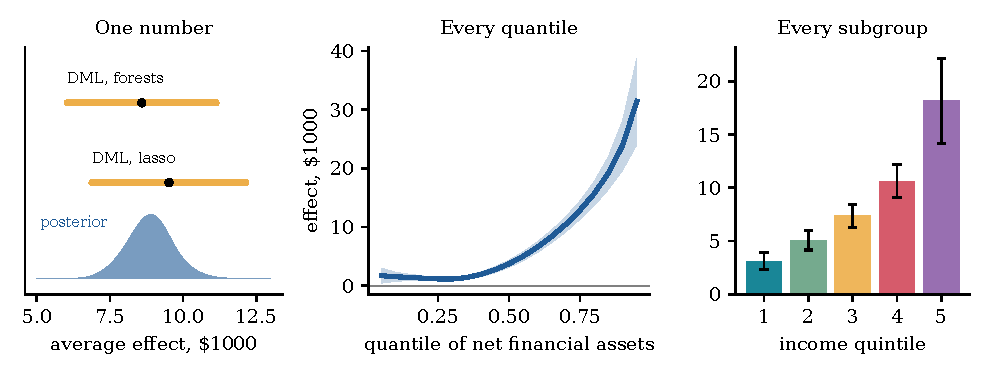
\includegraphics[width=\linewidth]{intro_onefit.pdf}
\caption{One model, many answers: 9{,}915 households in the 1991 SIPP, with the nine covariates of Section~\ref{sec:deephd}. Left: the two partially linear DML estimates of the effect of 401(k) eligibility on net financial assets (random forest and lasso nuisances) and their intervals (Table~\ref{tab:k401}), beside the approximate posterior of the average effect from 200 weighted Bayesian bootstrap refits of one quantile network. The partially linear estimates weight household effects by the conditional variance of eligibility given the covariates, and the network weights them equally; Section~\ref{sec:deephd} gives interactive DML estimates of the equally weighted average. Centre: the effect at every quantile of net financial assets. Right: the mean effect by income quintile. Centre and right come from the same draws as the posterior on the left, with bands of the mean plus or minus 1.96 standard deviations; in a simulation built to resemble these data, such a band covered the true average effect in 92 percent of 1,000 data sets drawn from a network of the same kind, and in 15 percent of 200 drawn from a truth outside that family (Section~\ref{sec:deephd}).}
\label{fig:intro}
\end{figure}

The causal reading of Figure~\ref{fig:intro} assumes that, given the nine recorded covariates, eligibility is as good as randomly assigned, with overlap, consistency and no interference between households (Section~\ref{sec:ignorability}). The centre panel then compares quantiles of the two potential asset distributions over the same households. It does not give the gain of the household at a particular wealth rank, which needs the further assumptions of Section~\ref{sec:ot}.

Neyman's potential outcomes and Rubin's Bayesian imputation already contain this idea. Three obstacles kept it from practice.

\paragraph{High dimensions.} With many covariates a prior must shrink, and a prior that shrinks the wrong coefficients shrinks away the confounding. The Robins and Ritov counterexample, long read as a proof that Bayesian causal inference fails in high dimensions, shows the same leak in another setting: independent priors on many sparsely observed cells that ignore how units were selected. We show that the failure belongs to the prior, not to Bayes. The horseshoe lets large effects through and shrinks noise hard. In our designs with five strong confounders, it leaves much less regularization induced confounding than the lasso. Coupling the outcome prior to a treatment regression fitted on the whole sample reduces it further with 50 and 150 covariates, though not with 300 (Chapters~\ref{ch:ipw} and~\ref{ch:horseshoe}). Shared scales also protect instruments, covariates that affect the outcome only through treatment, and leaving them unshrunk in the outcome regression inflates variance and, with residual confounding, amplifies bias (Section~\ref{sec:sharedsim}).

In our simulation of Section~\ref{sec:ricsim}, with 200 observations and 50 covariates the coupled posterior matches least squares, which needs no regularization there, and trails DML slightly on the average effect (root mean squared error 0.084 against DML's 0.079); the 95 percent intervals of DML and of the posterior both cover the truth in about 92 percent of 500 data sets, and the posterior also gives every other summary. With 150 and with 300 covariates among the same 200 observations and the same five confounders DML is the more accurate (root mean squared error 0.096 against DML's 0.080, and 0.124 against 0.084), and the coupling gains nothing in accuracy over the independent horseshoe that the data can resolve. With thirty weak confounders among 150 covariates the order reverses: the coupled posterior is the more accurate (root mean squared error 0.113 against DML's 0.126), and its intervals cover the truth in 94 percent of the data sets against DML's 76 percent. With 300 observations and 400 covariates the comparison with a reduced form posterior (with horseshoe priors on the coefficients of the treatment and marginal outcome regressions) is mixed: DML with a cross validated lasso has the smaller bias when confounding is sparse and overlap is good, and when it is dense no procedure covers (Chapter~\ref{ch:critique}).

\paragraph{Computation.} A posterior takes thousands of Markov chain iterations where DML takes a handful of regressions, and for the horseshoe models of this book the difference is seconds: the Gibbs sampler fits the 401(k) data, 9,915 households and 56 columns, in under a second on one core (Chapter~\ref{ch:computation}).

Where the likelihood cannot be evaluated cheaply, generative Bayesian computation turns posterior computation into supervised learning (Polson and Sokolov 2023, 2026a; Nareklishvili, Polson and Sokolov 2023a). A quantile neural network trained on simulations from the model maps uniform noise and a summary of the data to draws from the posterior given that summary, and each new data set from the same design costs a forward pass per draw. The training is the expense, more than an hour per network in our horseshoe experiment, so it pays only over many data sets from one design, and for the horseshoe the sampler won. 

Chapter~\ref{ch:gente} fits the network to the observed outcomes for distributional effects. Deep partial least squares projects many covariates onto a few directions first; with 200 irrelevant covariates added to the 401(k) data it helped, but it did not recover the nine covariate answer (Section~\ref{sec:deephd}).

\paragraph{Identification.} The probability that treatment caused a particular outcome depends on how a unit's two potential outcomes are coupled and cannot be identified from their margins, which is all trials and observational studies see. Report a posterior inside the Tian and Pearl bounds, separating what more data could narrow from what only the prior fixes (Chapter~\ref{ch:tianpearl}).

The payoff of working with one posterior is decisions. A posterior gives the probability that a programme helps, the action that maximizes expected utility, and risk sensitive alternatives for a planner who cares about the worst off, all from the same draws (Chapter~\ref{ch:cdt}). We work one decision in full: whether a merger raises prices, estimated with a Bayesian version of the BLP demand model in which the conduct of firms is itself uncertain (Chapter~\ref{ch:blp}).



\part{Foundations}
\chapter{Causal Questions}\label{ch:predictive}

\begin{tcolorbox}[colback=gray!6,colframe=gray!50,title=In brief,fonttitle=\normalfont\itshape,coltitle=black,colbacktitle=gray!15,boxrule=0.4pt,arc=1pt]
Causal questions are predictions about outcomes that were not observed. De Finetti's theorem turns a judgement of exchangeability into a model with a prior, ignorability says which part of that model the data inform, and every causal target, from the average effect to an individual attribution, is a functional of one posterior.
\end{tcolorbox}

In the spring of 1930 the Department of Health for Scotland gave about 10,000 schoolchildren in Lanarkshire\index{Lanarkshire milk experiment} three quarters of a pint of milk a day, from February to June, and kept about 10,000 more as controls. Every child was weighed and measured at the start and the end, so each child's growth is seen with milk or without it, and never both. Children were to be allocated by ballot or by alphabet, but teachers could substitute children when the groups looked unbalanced, and at the start the controls were already ahead by about three months' growth in weight and four in height. The gap in growth between the two groups mixes what milk does with how the teachers chose\index{confounding|textbf}\index{confounder|see{confounding}} (Section~\ref{sec:milk} tells the story at length).

A health authority deciding whether to pay for milk next year wants a forecast of next year's growth with milk and without it. A parent wants to know whether milk made the difference for her own child. One posterior answers both once we say which children are exchangeable and how they were assigned, though the parent's answer leans on a prior for something no experiment can show.





\section{Potential outcomes}\label{sec:potential}

Consider units $i = 1, \ldots, n$. Each unit has covariates $X_i$, receives a binary treatment $T_i \in \{0,1\}$, and has two potential outcomes\index{potential outcomes|textbf}\index{Rubin causal model|see{potential outcomes}}, $Y_i(1)$ if treated and $Y_i(0)$ if not. Only one of the two is ever observed:
\begin{equation}
Y_i = T_i Y_i(1) + (1 - T_i) Y_i(0).
\label{eq:consistency}
\end{equation}
Equation~\eqref{eq:consistency}, the consistency assumption\index{consistency assumption|textbf}, says the observed outcome equals the potential outcome for the treatment actually received. Implicit in the notation is the stable unit treatment value assumption: unit $i$'s outcomes do not depend on other units' treatments, and each treatment has only one version.

The missing outcome is the whole problem, what Holland\index{Holland, Paul W.!fundamental problem of causal inference|textbf} called the fundamental problem of causal inference\index{fundamental problem of causal inference|textbf}. Rubin\index{Rubin, Donald B.|textbf}'s insight was that this is a missing data\index{missing data|textbf} problem, and a Bayesian treats missing data through its posterior predictive distribution given everything observed.

\begin{definition}[Unit level and population effects]
The unit level effect\index{unit level effect|textbf} is $\tau_i = Y_i(1) - Y_i(0)$. The finite population\index{finite population|textbf} average treatment effect is
\[
\tau_{\mathrm{fp}} = \frac{1}{n}\sum_{i=1}^n \{Y_i(1) - Y_i(0)\}.
\]
For a superpopulation\index{superpopulation|textbf} with law $P$ on $(X, Y(0), Y(1))$, the average treatment effect\index{average treatment effect|textbf}\index{ATE|see{average treatment effect}}\index{population average treatment effect|see{average treatment effect}} is $\tau = \E_P\{Y(1) - Y(0)\}$ and the conditional average treatment effect\index{conditional average treatment effect|textbf}\index{CATE|see{conditional average treatment effect}}\index{conditional effect|see{conditional average treatment effect}} at covariate value $x$ is $\tau(x) = \E_P\{Y(1) - Y(0) \mid X = x\}$.
\end{definition}

The finite population effect $\tau_{\mathrm{fp}}$ is a property of the $n$ units in hand, a function of quantities half of which are missing; $\tau$ is a property of the law that generated them. A Bayesian can report a posterior for either, and the two differ, because the finite population effect holds the observed half of the table fixed and is uncertain only about the missing half (Section~\ref{gr:sec:urn}).

\section{Exchangeability as the bridge}\label{sec:exchangeability}

The law $P$ has to come from somewhere. A frequentist posits it. A Bayesian builds it from a symmetry judgement about the units.

\begin{definition}[Exchangeability]
A sequence of random quantities $Z_1, Z_2, \ldots$ is exchangeable\index{exchangeability|textbf} if for every $n$ and every permutation $\sigma$ of $\{1, \ldots, n\}$,
\[
(Z_1, \ldots, Z_n) \overset{d}{=} (Z_{\sigma(1)}, \ldots, Z_{\sigma(n)}).
\]
\end{definition}

\begin{theorem}[de Finetti]
If $Z_1, Z_2, \ldots$ is an infinite exchangeable sequence\index{exchangeable sequence|see{exchangeability}} taking values in a Polish space, there is a unique probability measure $\Pi$ on the space of probability laws\index{de Finetti theorem@de Finetti's theorem|textbf}\index{de Finetti representation|see{de Finetti's theorem}}\index{representation theorem|see{de Finetti's theorem}} such that
\[
\Prob(Z_1 \in A_1, \ldots, Z_n \in A_n) = \int \prod_{i=1}^n F(A_i) \, \Pi(dF)
\]
for every $n$ and every measurable $A_1, \ldots, A_n$. The random law $F$ is the almost sure weak limit of the empirical distribution of $Z_1, \ldots, Z_n$.
\end{theorem}

The binary case is de Finetti (1937) and Appendix~\ref{app:background} states it; the general case is Hewitt and Savage (1955), and a proof of the statement above, including the limit of the empirical distribution, is in Kallenberg (2002).

Take $Z_i = (X_i, Y_i(0), Y_i(1))$. If we judge the units exchangeable\index{potential outcomes!and exchangeability|textbf} before treatment is assigned, they behave as independent draws from an unknown law $F$ with prior $\Pi$, and causal estimands\index{estimand} are functionals of $F$: $\tau = \tau(F)$, $\tau(x) = \tau(F; x)$, and so on. Exchangeability already implies the model.

When $F$ is indexed by a finite dimensional parameter $\theta$ we write the representation\index{de Finetti theorem@de Finetti's theorem} in the familiar form
\begin{equation}
p(z_1, \ldots, z_n) = \int \prod_{i=1}^n f(z_i \mid \theta) \, \pi(d\theta).
\label{eq:definetti}
\end{equation}
The predictive distribution of an unobserved potential outcome integrates $f$ against the posterior for $\theta$.

\begin{remark}
Exchangeability of the full triples is a different judgement from exchangeability of the observed records\index{exchangeability!of the observed records|textbf} $(X_i, T_i, Y_i)$: before treatment, nothing distinguishes the units except their covariates. Partial exchangeability\index{exchangeability!partial|textbf}, within groups defined by covariates, is the natural weakening and the judgement behind every regression model. Section~\ref{gr:sec:transform} adds the restriction that the treatment acts in the same way in every covariate cell, which gives the effect a group structure.
\end{remark}

Two other weakenings are common. Units may be exchangeable within schools, hospitals or regions, with the groups themselves exchangeable, which gives hierarchical models with group level parameters drawn from a common law. And regression coefficients may be exchangeable, or exchangeable within blocks, the judgement behind shrinkage priors such as the horseshoe (Chapter~\ref{ch:horseshoe}). Each judgement can be challenged, and the challenge is always substantive. A critic who doubts that two schools are exchangeable must say how they differ, and the answer becomes a covariate or a stratum in the model; disagreements about the model are then disagreements about the world.

\section{Assignment and ignorability}\label{sec:ignorability}

To learn about $F$ we must know how treatment was assigned. Write the assignment mechanism\index{assignment mechanism|textbf}\index{treatment assignment|see{assignment mechanism}} as $p(T \mid X, Y(0), Y(1), \phi)$, where $\phi$ indexes it.

\begin{definition}[Ignorability]\label{def:ignorability}
Treatment assignment is strongly ignorable\index{ignorability!strong|textbf}\index{ignorability}\index{strong ignorability|see{ignorability}} given $X$ if
\[
\{Y(0), Y(1)\} \indep T \mid X \quad\text{and}\quad 0 < e(x) < 1 \text{ for all } x,
\]
where $e(x) = \Prob(T = 1 \mid X = x)$ is the propensity score\index{propensity score|textbf}\index{overlap|textbf}\index{common support|see{overlap}}\index{positivity|see{overlap}}\label{def:propensity}.
\end{definition}


\begin{figure}[ht]
\centering
\begin{tikzpicture}[node distance=18mm]
\node[v] (X) {$X$};
\node[v,below left=of X] (T) {$T$};
\node[v,below right=of X] (Y) {$Y$};
\draw[e] (X) -- (T); \draw[e] (X) -- (Y); \draw[e] (T) -- (Y);
\end{tikzpicture}
\caption{Confounding by measured covariates. Ignorability holds given $X$, and every superpopulation and conditional effect is a functional of the law of $Y$ given $(X, T)$ averaged over a law of $X$.}
\label{fig:dagconf}
\end{figure}

For a Bayesian, ignorability\index{ignorability|textbf}\index{unconfoundedness|see{ignorability}} (Figure~\ref{fig:dagconf}) has a precise consequence. If the assignment vector depends on the potential outcomes only through the covariates, $p(t \mid x, y(0), y(1), \phi) = p(t \mid x, \phi)$, the joint density of the observed data factorizes as
\[
p(y, t \mid x, \theta, \phi) = p(t \mid x, \phi) \prod_{i=1}^n f(y_i \mid x_i, t_i, \theta).
\]
The assignment factor need not be a product over units; complete randomization, which fixes the number treated, is not. If $\theta$ and $\phi$ are a priori independent, the posterior for $\theta$ does not involve the assignment mechanism at all:
\begin{equation}
\pi(\theta \mid y, t, x) \propto \pi(\theta) \prod_{i=1}^n f(y_i \mid x_i, t_i, \theta).
\label{eq:ignorable}
\end{equation}
Rubin called this the ignorability of the assignment mechanism for Bayesian inference. Its most famous criticism\index{Robins and Ritov example} hinges on the phrase ``a priori independent'' (Section~\ref{sec:rrw}). When the analyst knows how selection relates to outcomes, the prior should say so, and then \eqref{eq:ignorable} no longer holds in that form.

\section{Three kinds of causal target}\label{sec:targets}

Three families of target\index{estimand|textbf}\index{estimand!choice of|textbf}\index{causal target|see{estimand}}\index{target of inference|see{estimand}} recur throughout the book.

\paragraph{Population averages.} The average treatment effect\index{average treatment effect} $\tau$, the effect on the treated $\E\{Y(1) - Y(0) \mid T = 1\}$, and their finite population versions average contrasts over units. The superpopulation versions are identified under ignorability and overlap. The finite population versions are not functionals of the law of the observed data: their posteriors also depend on the association between $Y(0)$ and $Y(1)$, which the data do not inform (Section~\ref{sec:imputation}).

\paragraph{Conditional and distributional effects.} The conditional effect $\tau(x)$, the quantile treatment effect\index{quantile treatment effect|textbf}\index{QTE|see{quantile treatment effect}}\index{quantile effect|see{quantile treatment effect}} $F_{Y(1)}^{-1}(u) - F_{Y(0)}^{-1}(u)$, and effects on any other feature of the marginal laws\index{distributional target|textbf} describe heterogeneity. They too are identified under ignorability, though estimating them well needs much more data than $\tau$.

\paragraph{Individual attributions.} The probability that treatment was necessary for an outcome\index{probabilities of causation}, $\Prob\{Y(0) = 0 \mid T = 1, Y = 1\}$, or that it was both necessary and sufficient, $\Prob\{Y(1) = 1, Y(0) = 0\}$, depend on the joint law of $Y(0)$ and $Y(1)$. No experiment observes both potential outcomes for one unit, so without further assumptions such as monotonicity they are not identified and can only be bounded; Chapter~\ref{ch:tianpearl} is devoted to them.

Suppose a randomized experiment\index{randomized experiment|textbf}\index{randomized trial|see{randomized experiment}} shows $p_1 = \Prob\{Y(1) = 1\} = 0.6$ and $p_0 = \Prob\{Y(0) = 1\} = 0.3$. The probability of necessity and sufficiency\index{probability of necessity and sufficiency}, $\mathrm{PNS} = \Prob\{Y(1) = 1, Y(0) = 0\}$, then satisfies
\[
\max(0, p_1 - p_0) \le \mathrm{PNS} \le \min(p_1, 1 - p_0),
\]
which here is $0.3 \le \mathrm{PNS} \le 0.6$. The lower end, $p_1 - p_0$, is the proportion helped minus the proportion harmed, and PNS reaches it when treatment harms no one; the upper end holds because PNS cannot exceed the probability of either event it combines. The experiment fixes the two margins and leaves their coupling free, so an interval of width 0.3 is all it can say. Section~\ref{gr:sec:margins} says which quantities the two margins identify and which they leave free.

A framework with no way to state the third kind of question is, in our view, incomplete. Courts ask it daily: was this plaintiff's cancer caused by the defendant's product? The answer depends on the joint law of the two potential outcomes, which the data never reveal, so double machine learning (DML) has no point to estimate. It can estimate the identified bounds (Chapter~\ref{ch:tianpearl}); a posterior over a joint model can also represent what is known and what is not.

\section{A first worked example}\label{sec:firstexample}

Consider the Gaussian linear model\index{Gaussian linear model|textbf}
\[
Y(t) = \alpha + \tau t + \beta^\top X + \varepsilon_t, \qquad \varepsilon_t \sim N(0, \sigma^2),
\]
with treatment assigned completely at random. Place a flat prior\index{prior distribution!flat|textbf} on $(\alpha, \tau, \beta)$ and Jeffreys' prior\index{prior distribution!Jeffreys|textbf} on $\sigma^2$. The marginal posterior of $\tau$ is then a scaled Student $t$ distribution centred at the least squares coefficient, with $n - p - 2$ degrees of freedom, where $p$ is the dimension of $X$. The posterior is proper when the design matrix with rows $(1, T_i, X_i^\top)$ has full column rank, $n > p + 2$ and the least squares residuals are not all zero, and its variance is finite when $n > p + 4$.

This is classical analysis of covariance\index{analysis of covariance|textbf}\index{ANCOVA|see{analysis of covariance}}. With no interactions, $\tau(x) = \tau$ for all $x$, so the posterior of $\tau$ is the posterior of the average treatment effect for any covariate population. Add an interaction $\gamma^\top X t$ and $\tau(x) = \tau + \gamma^\top x$, so the coefficient $\tau$ is now the effect at $x = 0$ and the average treatment effect depends on which population of $x$ we average over. The data have not changed; the model has, and with it the accounting. A new covariate law $Q$ needs no new fit, only a new average at each posterior draw:
\[
\tau_Q = \int \tau(x)\,Q(dx) = \tau + \gamma^\top \E_Q X.
\]



\section{Prediction, decision and policy}\label{sec:policyvalue}

Causal questions are asked in order to act. The health authority of the opening must decide whether to pay for milk for everyone, for no one, or for a targeted subgroup, and wants next year's growth under each policy; a patient deciding whether to quit smoking wants her own risk under each choice. Both are predictive distributions for future observables under an intervention, forecasts that are scored when the outcomes arrive.

Dawid's decision theoretic account uses a regime indicator\index{regime indicator} $F_T$ that is $\emptyset$ for the observational regime and $t$ when treatment is set to $t$: the causal effect compares $p(Y \mid F_T = 1)$ with $p(Y \mid F_T = 0)$, and ignorability says the conditional law of $Y$ given $X$ and $T$ is the same in the observational and interventional regimes (Chapter~\ref{ch:frameworks}). Superpopulation and conditional effects need no counterfactuals, since each is a feature of the law of an observable under a regime that could in principle be run; the finite population effect, individual attributions and natural direct and indirect effects do.

Each policy $\delta$ maps covariates to treatment, and its value\index{policy value|textbf}\index{treatment policy|see{policy value}} is the expected outcome of a future patient under the policy,
\[
V(\delta) = \int \E\{Y(\delta(x)) \mid X = x\}\,Q(dx),
\]
where $Q$ is the covariate law of future patients. Under ignorability, and if the conditional law of the outcome carries over from the study to the future patients (Section~\ref{fw:sec:transport}), given $\theta$ it is $V(\delta;\theta) = \int \mu_{\delta(x)}(x;\theta)\,Q(dx)$, with $\mu_t(x;\theta) = \E(Y \mid X = x, T = t, \theta)$ the outcome regression. Evaluating $V(\delta;\theta)$ at each posterior draw gives its posterior; averaging gives the posterior predictive mean outcome under $\delta$. The Bayes optimal policy\index{policy value!optimal policy|textbf} maximizes posterior expected value, possibly penalized by cost.

In the worked example of Section~\ref{sec:firstexample}, let treating a patient cost $c$ on the outcome scale. Given $\theta$ and without an interaction, every policy that treats a fraction $w$ of the population has value net of cost $\alpha + \beta^\top \E_Q X + w(\tau - c)$, and the best policy treats everyone if $\tau$ exceeds $c$ and no one otherwise; the average effect is all that matters. With the interaction $\gamma^\top X t$, treating the subgroup\index{subgroup effect|textbf} $\{x : \delta(x) = 1\}$ adds $\int_{\delta = 1} (\tau + \gamma^\top x - c)\,Q(dx)$ to the value net of cost of treating no one, and the best policy given $\theta$ treats exactly those $x$ at which $\tau + \gamma^\top x$ exceeds $c$. The Bayes policy replaces $\tau + \gamma^\top x$ by its posterior mean (Exercise~\ref{ex:ch01:7}). A method that reports only $\tau$ cannot find that policy, and a method that reports $\tau(x)$ without its posterior uncertainty cannot say how confident the authority should be in the boundary it draws. The posterior draws $\theta^{(s)}$ give both: for each draw, the value of every candidate policy, and across draws, the probability that one policy beats another.

\section{Posterior predictive imputation}\label{sec:imputation}

The Bayesian computation of a finite population effect\index{finite population effect|textbf}\index{sample average treatment effect|see{finite population effect}} is an imputation\index{imputation|textbf}\index{imputation!posterior predictive|textbf}\index{posterior predictive imputation|see{imputation}} algorithm.

\begin{enumerate}
\item Specify a joint model $f(y(0), y(1) \mid x, \theta)$ for the pair of potential outcomes given covariates, and a prior $\pi(\theta)$.
\item Under ignorability, obtain draws $\theta^{(1)}, \ldots, \theta^{(S)}$ from the posterior, which depends only on the observed outcome of each unit and the marginal of $f$ for that arm.
\item For each draw $s$ and each unit $i$, draw the missing potential outcome\index{imputation!of missing potential outcomes|textbf} from its conditional law given the observed one: $Y_i^{\mathrm{mis}} \sim f(y(1 - T_i) \mid y(T_i) = Y_i, x_i, \theta^{(s)})$.
\item Compute any finite population\index{finite population} summary of the completed table, for example $\tau_{\mathrm{fp}}^{(s)} = n^{-1}\sum_i\{Y_i(1) - Y_i(0)\}^{(s)}$.
\end{enumerate}

Step 3 needs the conditional law of one potential outcome given the other, which depends on their association, and that association is not identified (Section~\ref{sec:ot}). Superpopulation targets skip step 3, since $\tau(\theta)$ depends only on the marginals. Chapter~\ref{ch:computation} shows how to obtain the draws of step 2, by Markov chain Monte Carlo or by the Generative Bayesian Computation of Polson and Sokolov (2026a). No sampler helps with step 3: the association is absent from the observed data likelihood, so when its prior is independent of the marginal parameters its posterior is that prior.

\begin{proposition}
Under ignorability, in the bivariate normal model with $Y(t) \mid x \sim N(\mu_t(x), \sigma_t^2)$ and correlation $\rho$ between $Y(0)$ and $Y(1)$, the conditional posterior variance of $\tau_{\mathrm{fp}}$ given $\theta$ is
\[
\frac{1}{n^2}\sum_{i=1}^n \sigma_{1 - T_i}^2(1 - \rho^2).
\]
\end{proposition}

\begin{proof}
Given $\theta$, the missing outcome of unit $i$, with $t = T_i$, is
\[
Y_i^{\mathrm{mis}} \mid \theta, Y_i \sim N\!\left(\mu_{1-t}(x_i) + \rho\,\frac{\sigma_{1-t}}{\sigma_t}\{Y_i - \mu_t(x_i)\},\ \sigma_{1-t}^2(1 - \rho^2)\right),
\]
independently across units. Each missing outcome enters $\tau_{\mathrm{fp}}$ with coefficient $\pm 1/n$; the observed outcomes are fixed, so the variances add.
\end{proof}

At $\rho = \pm 1$ the conditional variance above vanishes, because the observed outcome determines the missing one; at $\rho = 0$ it is largest. The posterior of $\theta$ adds the variance of the conditional mean of $\tau_{\mathrm{fp}}$, and in the two arm model without covariates, with known variances and flat priors on the two means, the two pieces sum to
\[
\mathrm{Var}(\tau_{\mathrm{fp}} \mid \text{data}) = \mathrm{Var}(\tau \mid \text{data}) - \frac{\sigma_1^2 + \sigma_0^2 - 2\rho\sigma_0\sigma_1}{n},
\]
as Exercise~\ref{ex:ch01:3} derives. The subtracted term is the variance of the unit effects divided by $n$. Thus the posterior variance of $\tau_{\mathrm{fp}}$ is no larger than that of $\tau$\index{average treatment effect!posterior of|textbf} and increases with $\rho$. With known variances and $n_t$ units in arm $t$, Neyman's conservative variance\index{Neyman conservative variance estimator@Neyman's conservative variance estimator|textbf}, $\sigma_1^2/n_1 + \sigma_0^2/n_0$, equals $\mathrm{Var}(\tau \mid \text{data})$. The finite population variance reaches this bound only when $\rho = 1$ and $\sigma_0 = \sigma_1$. With unequal standard deviations, even its maximum at $\rho = 1$ falls below the bound by $(\sigma_1-\sigma_0)^2/n$. For binary outcomes Proposition~\ref{gr:prop:sharpvar} shows that the bound is never sharp when $0 < |\tau_{\mathrm{fp}}| < 1$.

Take $n = 100$ with 50 units in each arm and both standard deviations equal to 1. The posterior variance of $\tau$ is $1/50 + 1/50 = 0.040$, and that of $\tau_{\mathrm{fp}}$ is $0.040 - 0.02(1 - \rho)$, which is $0$, $0.010$, $0.020$, $0.030$ and $0.040$ at $\rho = -1$, $-0.5$, $0$, $0.5$ and $1$. At $\rho = -0.5$ the posterior standard deviation of $\tau_{\mathrm{fp}}$ is half that of $\tau$. The data cannot say which of these values applies, so the Bayesian states a prior for $\rho$ and reports the finite population interval under it; Neyman's conservative interval is the one for $\rho = 1$.

\section{Interference}\label{sec:interference}

The stable unit treatment value assumption\index{stable unit treatment value assumption|textbf}\index{SUTVA|see{stable unit treatment value assumption}} fails whenever one unit's treatment affects another's outcome\index{interference|textbf}. Three examples recur.

\paragraph{Vaccination.} A vaccinated person protects the unvaccinated people around her. The effect of vaccinating one person depends on how many others are vaccinated, so the population effect of a campaign is not the sum of individual effects.

\paragraph{Classrooms.} If milk made treated Lanarkshire children more energetic or attentive, their untreated classmates might have been affected too, and the experiment was not designed to detect such spillovers\index{spillover|see{interference}}.

\paragraph{Markets.} A training programme that raises some workers' skills may lower the wages of untrained workers who compete with them. The partial equilibrium effect from a small trial can differ from the general equilibrium effect of scaling up.

A Bayesian handles interference by modelling it. Potential outcomes become functions of the whole treatment vector, $Y_i(t_1, \ldots, t_n)$, and the model restricts the dependence, for example to the proportion treated in the unit's cluster. If units are exchangeable within clusters and the clusters themselves are exchangeable, and both judgements extend to arbitrarily many units and clusters, de Finetti's theorem\index{de Finetti theorem@de Finetti's theorem} applied to the clusters gives a hierarchical model, as in Section~\ref{sec:exchangeability}.

Assume interference only within clusters. A coverage $a \in (0,1)$ is an allocation policy: each unit in a cluster is treated independently with probability $a$. Write $\bar Y(t; a)$ for the mean outcome of a unit given treatment $t$ while its clustermates are assigned under coverage $a$, averaged over units and over the clustermates' assignments. Three targets adapt those of Hudgens and Halloran (2008), whose two stage design fixes the number treated in each cluster: the direct effect $\bar Y(1; a) - \bar Y(0; a)$, the spillover (their indirect) effect $\bar Y(0; a') - \bar Y(0; a)$ of raising coverage from $a$ to $a'$, and the overall effect
\[
\bar Y(a') - \bar Y(a), \qquad \bar Y(a) = a\,\bar Y(1; a) + (1 - a)\,\bar Y(0; a).
\]
Randomizing clusters to coverages and then units within clusters (two stage randomization) identifies each $\bar Y(t; a)$ as an observed arm mean at that coverage; individual level ignorability alone does not. A model for $Y_i$ given its own treatment and its cluster's coverage then gives each target as a functional of its posterior draws.

\section{In practice}\label{sec:inpractice}

\paragraph{The target.} Given posterior draws $\theta^{(1)}, \ldots, \theta^{(S)}$ and an outcome model $f(y \mid x, t, \theta)$, every target in this chapter is a function of those draws. The conditional effect at $x$ is $\mu_1(x;\theta^{(s)}) - \mu_0(x;\theta^{(s)})$, with $\mu_t$ the outcome regression of Section~\ref{sec:policyvalue}; the superpopulation effect averages it over the covariate law of the superpopulation; the finite population effect imputes the missing outcomes and averages the completed table; an individual attribution also needs a joint model for the pair of potential outcomes, and its posterior carries the prior on the part the data cannot inform.

\paragraph{What the analyst does differently.} The analyst states three things before fitting anything. The exchangeability judgement: which units are exchangeable with which, and given what covariates, since that judgement is the model. The assignment mechanism: for randomized assignment or assignment based only on recorded covariates, \eqref{eq:ignorable} applies if the prior keeps $\theta$ and $\phi$ independent. If selection is known to relate to outcomes, the prior must link $\theta$ and $\phi$. If assignment depended on unrecorded predictors of the outcome, the assignment model stays in the likelihood and its unidentified part calls for a sensitivity analysis (Section~\ref{sec:sensitivity}). And the target, including the population $Q$ it averages over. She then fits one model and checks it by its posterior predictive against the observed outcomes, a check that can reject the outcome model but cannot confirm ignorability or inform $\rho$. She reports the posterior of each target the decision needs, labelling the finite population effect and any individual attribution as depending on an unidentified association ($\rho$ in the Gaussian example).

\paragraph{Against DML.} DML takes the identification of this chapter as given and estimates one functional, usually $\tau$, with a confidence interval. For that one number in a large sample with ignorable assignment it is adequate and cheap. The same cross fitted nuisance estimates can also value a fixed subgroup policy through doubly robust scores, as in Athey and Wager (2021), and stacking scores gives joint intervals for a few functionals named in advance; each needs its own score and its own asymptotic argument.  An unrestricted conditional effect curve $\tau(x)$ with uncertainty joint with $\tau$ needs a separate nonparametric estimator, the value of a policy chosen from the same data needs further conditions, and the finite population effect and individual attributions depend on the coupling of the potential outcomes, which no score identifies. In the Bayesian analysis each is one more functional of the same posterior draws, with the coupling stated as a prior where the target needs it.

The Bayesian analysis is not automatically efficient, and with many covariates it needs a prior built for the dimension and, where selection matters, perhaps a propensity aware prior; Chapters~\ref{ch:critique} and~\ref{ch:horseshoe} test that with numbers. In our designs with five strong confounders among 50, 150 and 300 covariates (Section~\ref{sec:ricsim}), the horseshoe coupled to a fitted treatment regression gains over the independent horseshoe at $p = 50$, a gain the simulations do not resolve at $p = 150$ or $300$, and DML is more accurate than either for the average effect in all three, so the case for the Bayesian analysis rests on what it returns, a posterior for every target, and not on accuracy for one number.

\section*{Notes}

Potential outcomes for randomized experiments are due to Neyman (1923, translated 1990), and Rubin (1974) carried the notation to observational studies. The Bayesian reading of this chapter, in which missing outcomes are imputed from their posterior predictive distribution and an ignorable assignment mechanism drops out of the posterior, is Rubin (1978). Rosenbaum and Rubin (1983) introduced strong ignorability, and Holland (1986) named the fundamental problem of causal inference. Imbens and Rubin (2015) develop the finite population and superpopulation views, with Neyman's conservative variance, at book length.

Diaconis and Freedman (1980) bound how far the first few variables of a long finite exchangeable sequence are from a mixture of independent and identically distributed ones (Exercise~\ref{ex:ch01:4}). Heath and Sudderth (1976) give the urn form used in Section~\ref{gr:sec:urn}. The regime indicator is from Dawid (2002, 2015, 2021); Athey and Wager (2021) study the value of a policy learned from observational data. Tian and Pearl (2000) derive the bounds on the probability of necessity and sufficiency. Robins and Ritov (1997) criticize Bayesian ignorability. Hudgens and Halloran (2008) define direct and spillover effects under interference confined to clusters.



\begin{exercises}
\item\label{ex:ch01:1} Show that under complete randomization the difference in sample means is unbiased for $\tau_{\mathrm{fp}}$ over the randomization distribution, and derive Neyman's conservative variance estimator.
\item\label{ex:ch01:2} In the Gaussian model with interaction $\gamma^\top X t$, with a flat prior on all coefficients and Jeffreys' prior on $\sigma^2$, write down the posterior of the average treatment effect for the covariate law $Q$ and show that its posterior variance depends on $Q$ only through the mean of $X$ under $Q$.
\item\label{ex:ch01:3} Let $Y(0)$ and $Y(1)$ be bivariate normal with standard deviations $\sigma_0$ and $\sigma_1$ and correlation $\rho$. Show that the posterior variance of $\tau_{\mathrm{fp}}$ given $\theta$ is decreasing in $|\rho|$, that in the two arm model without covariates, with known variances and flat priors on the means, its unconditional posterior variance is that of $\tau$ minus $(\sigma_1^2+\sigma_0^2-2\rho\sigma_0\sigma_1)/n$, and identify which value of $\rho$ makes Neyman's variance estimator exact when $\sigma_1 = \sigma_0$.
\item\label{ex:ch01:4} Give an example of a finite exchangeable sequence that is not a mixture of independent and identically distributed sequences, and explain why this does not affect the argument of Section~\ref{sec:exchangeability} when the units in hand are few relative to the population, and why it does matter for a target that averages over the whole population.
\item\label{ex:ch01:6} Construct a two unit example in which the stable unit treatment value assumption fails, and show that $\tau_i$ is then not well defined without specifying the treatment of the other unit.
\item\label{ex:ch01:7} In the Gaussian model with interaction $\gamma^\top X t$, let treating a patient cost $c$ and judge a policy $\delta$ by its value net of cost. Show that the policy with the highest posterior expected value treats exactly the patients $x$ with $\E(\tau + \gamma^\top x \mid \text{data}) > c$. For this policy $\delta^\ast$ and any fixed policy $\delta$, show that $V(\delta^\ast) - V(\delta)$ is affine in $(\tau, \gamma)$, and write the posterior probability that $\delta^\ast$ beats treating no one, first for a normal posterior of $(\tau, \gamma)$ and then as an average over posterior draws.
\item\label{ex:ch01:8} Let $p_1 = \Prob\{Y(1) = 1\}$ and $p_0 = \Prob\{Y(0) = 1\}$. Show that $\max(0, p_1 - p_0) \le \Prob\{Y(1) = 1, Y(0) = 0\} \le \min(p_1, 1 - p_0)$, that each end is reached by some joint law of $(Y(0), Y(1))$ with these margins, and that when $p_1 \ge p_0$ the lower end is the value exactly when no unit has $Y(1) = 0$ and $Y(0) = 1$.
\item\label{ex:ch01:9} Take a two arm table with $n = 100$ and 50 units in each arm, any observed outcomes, flat priors on the two means and known standard deviations $\sigma_1 = \sigma_0 = 1$. For $\rho$ in $\{-1, -0.5, 0, 0.5, 1\}$, draw $(\mu_0, \mu_1)$ from their posterior, impute each missing outcome from its conditional law given the observed one, and record the variance across draws of $\tau_{\mathrm{fp}}$ and of $\tau = \mu_1 - \mu_0$. Compare both with the formula of Section~\ref{sec:imputation} and Exercise~\ref{ex:ch01:3}, and repeat with $\sigma_0 = 2$ to see that the two variances differ even at $\rho = 1$.
\end{exercises}

\chapter{Frameworks for Causal Inference}\label{ch:frameworks}

\begin{tcolorbox}[colback=gray!6,colframe=gray!50,title=In brief,fonttitle=\normalfont\itshape,coltitle=black,colbacktitle=gray!15,boxrule=0.4pt,arc=1pt]
The frameworks of Fisher, Neyman and Rubin, Pearl, Robins, Dawid and the econometricians differ on what a cause is and on where identification comes from, design in a randomized experiment and assumption everywhere else, yet they largely compute the same estimators. A reader who wants the Bayesian development can skip the chapter on a first reading and return to it when a later chapter cites one of the frameworks.
\end{tcolorbox}

Causal inference has no single theory. It has a family of theories that agree on the questions (does this drug lower mortality, does this policy raise employment) but disagree on almost everything else: what a causal claim asserts, what mathematical object encodes it, which assumptions license it, and whether the usual estimands are even the right targets. Whether one writes an effect as a counterfactual or as an intervention, and whether one targets a marginal or a conditional effect, changes both what may be claimed and how the claim must be defended.

A causal conclusion can be earned by design\index{design versus assumption} or by assumption. In a randomized experiment the causal reading follows from how the data were generated. As Harrell (2026) puts it, with no interruption in the flow of data ``there is no explanation for the result other than the experimental manipulation and random variation.'' In an observational study, identification rests on an untestable premise, such as no unmeasured confounding, a valid instrument, parallel trends or continuity at a threshold. The conclusion is as credible as that premise. The frameworks largely agree on the arithmetic; they dispute the meaning and provenance of the assumptions.

\section[The fundamental problem]{The fundamental problem and the language of causation}\label{fw:sec:fundamental}

Almost every modern framework begins, explicitly or implicitly, with the pair of potential outcomes\index{potential outcomes} $\{Y_i(0), Y_i(1)\}$ of a unit $i$ under a binary treatment $T_i \in \{0,1\}$, tied to the observed outcome by the consistency identity \eqref{eq:consistency} of Chapter~\ref{ch:predictive}. The unit effect $\tau_i = Y_i(1) - Y_i(0)$ is never directly observed, so attention shifts to population summaries, chiefly the average treatment effect and the effect on the treated. The naive contrast of observed group means estimates neither in general, but
\begin{equation}\label{fw:eq:decomp}
\begin{split}
\E[Y \mid T=1] - \E[Y \mid T=0] &= \underbrace{\E[Y(1)-Y(0)\mid T=1]}_{\text{effect on the treated}}\\
&\quad + \underbrace{\E[Y(0)\mid T=1] - \E[Y(0)\mid T=0]}_{\text{selection bias}}.
\end{split}
\end{equation}
The second term is selection bias\index{selection bias|textbf}, or confounding, and it is what the field is about. Every framework is a strategy for it: argue that it is zero by design, or estimate and remove it by assumption.

Holland\index{Holland, Paul W.!fundamental problem of causal inference} (1986), who named the fundamental problem\index{fundamental problem of causal inference}, attached the slogan ``no causation without manipulation''\index{no causation without manipulation|textbf}: a cause must be, at least conceptually, a potential intervention, which excludes immutable attributes such as sex.

The potential outcome notation is not theory neutral. Writing $\{Y(0), Y(1)\}$ as a pair of random variables commits one to a joint distribution over counterfactuals\index{counterfactual|textbf}, including the cross world dependence $\Cov(Y(0), Y(1))$, which no experiment can identify. Dawid's framework (Section~\ref{fw:sec:dawid}) targets exactly this commitment, and Section~\ref{sec:ot} and Chapter~\ref{ch:tianpearl} show what follows when one keeps it and puts a prior on the unidentified coupling.

\section{Fisher: randomization as the reasoned basis for inference}\label{fw:sec:fisher}

The oldest of the modern frameworks is also the most austere. Fisher\index{Fisher, Ronald A.|textbf} (1925, 1935) made physical randomization\index{randomization} the foundation of experimental inference\index{Fisher, Ronald A.!randomization|textbf}\index{randomized experiment}. He did not claim that randomization makes groups equal (in any finite sample they differ on countless covariates), but that it furnishes the probability distribution against which an observed contrast is judged: ``the reasoned basis for inference\index{randomization!as the basis of inference|textbf}.''

Fisher's test addresses the sharp null hypothesis\index{sharp null|textbf}\index{Fisher, Ronald A.!sharp null|textbf} of no effect for any unit,
\[
H_0:\quad Y_i(1) = Y_i(0) \quad\text{for all } i.
\]
Under $H_0$ the missing outcome equals the observed one, so the only randomness is the assignment, whose distribution the experimenter controls. Enumerating or sampling the assignments the design allows gives the exact reference distribution of any test statistic, without parametric assumptions. In the lady tasting tea\index{lady tasting tea|textbf}, the number of correct identifications under the sharp null is hypergeometric, and the $p$ value is a combinatorial fact.

The randomization test\index{randomization test|textbf} is essentially assumption free for the sharp null, but, as Neyman stressed, it tests that null rather than estimating an effect. It does not by itself deliver intervals, random effects, longitudinal or Bayesian machinery.

The fault line that still divides the field opened at the Royal Statistical Society in 1935, when Neyman presented his analysis of randomized blocks (Neyman, Iwaszkiewicz and Kolodziejczyk 1935) and Fisher responded with characteristic ferocity. Fisher's sharp null against Neyman's weak null of no average effect is a disagreement about the object of inference, which functional of the completed table of potential outcomes is the target. A treatment with exactly zero average effect may help half the units and harm the other half, making the sharp null false and the weak null true.

In the smoking and lung cancer controversy (Chapter~\ref{ch:smoking}) Fisher pressed a common constitutional cause of both the habit and the cancer, dramatizing his doctrine that without randomization a confounder can always be hypothesized.

\section{Neyman and Rubin: potential outcomes and the assignment mechanism}\label{fw:sec:rubin}

Neyman\index{Neyman, Jerzy|textbf} (1923) represented each plot by its yield under each variety\index{Neyman, Jerzy!potential outcomes|textbf}; randomization selects the observed yield. He derived the unbiasedness of the difference in means\index{difference in means|textbf} over randomization and the conservative variance estimator\index{Neyman conservative variance estimator@Neyman's conservative variance estimator} for the average effect $\tau_{\mathrm{fp}}$ of Chapter~\ref{ch:predictive}. Rubin\index{Rubin, Donald B.} (1974, 1978) extended the notation to observational studies\index{Rubin, Donald B.!potential outcomes|textbf} and made the assignment mechanism\index{assignment mechanism} explicit in what Holland\index{Holland, Paul W.!Rubin causal model|textbf} (1986) named the Rubin causal model\index{potential outcomes!Neyman and Rubin tradition|textbf}. Under market equilibrium, a policy applied at scale changes prices for every unit, violating the stable unit treatment value assumption (Chapter~\ref{ch:predictive}).

The assignment mechanism $\Prob(T \mid Y(0), Y(1), X)$ is known in a randomized experiment and assumed in an observational study. Under the strong ignorability\index{ignorability}\index{ignorability!in the Rubin framework|textbf} of Chapter~\ref{ch:predictive}, $\E[Y(t)] = \E_X[\E(Y \mid T=t, X)]$, so the average effect is identified by averaging conditional regressions over the covariate distribution, the adjustment or g formula.

Rosenbaum\index{Rosenbaum, Paul R.!propensity score} and Rubin\index{Rubin, Donald B.!propensity score} (1983), who introduced strong ignorability, proved that the propensity score\index{propensity score} $e(X) = \Prob(T=1 \mid X)$ is a balancing score, $X \indep T \mid e(X)$, and that ignorability given $X$ implies it given $e(X)$ alone. The score presupposes ignorability and cannot manufacture it, and, as Rubin stresses, the design of an observational study, choosing and balancing covariates, can and should be done without seeing the outcomes.

The Rubin causal model is ecumenical about inference, admitting Fisherian randomization tests, Neymanian repeated sampling and Bayesian imputation. In the Bayesian mode (Rubin 1978) one places a model on the science $\Prob(Y(0), Y(1)\mid X,\theta)$ and a prior on $\theta$, imputes the missing potential outcomes from their posterior predictive distribution and reads any estimand off the completed table. An ignorable assignment mechanism whose parameters are a priori independent of $\theta$ then drops out of the posterior \eqref{eq:ignorable}. 

\section{Pearl: structural causal models and the do calculus}\label{fw:sec:pearl}

Where the Rubin model starts from potential outcomes and treats causal structure as an assumption about assignment, Pearl\index{Pearl, Judea|textbf} (1995, 2009) starts from the structure itself, encoded as a directed acyclic graph\index{directed acyclic graph|textbf}\index{DAG|see{directed acyclic graph}}, and derives potential outcomes from it. A structural causal model\index{structural causal model|textbf}\index{Pearl, Judea!structural causal models|textbf} is a system of nonparametric structural equations\index{structural equation}
\[
V_j = f_j\bigl(\mathrm{pa}(V_j),\, U_j\bigr), \qquad j = 1,\dots,d,
\]
one per variable, with $\mathrm{pa}(V_j)$ its graphical parents and $U_j$ exogenous noise. The equations are assignments: reading the equals sign as ``is computed from'' distinguishes a structural equation from a regression. For identifying the effect of a single treatment the Rubin and Pearl languages are interchangeable: a structural model defines potential outcomes\index{potential outcomes!and structural equations|textbf}, and ignorability assumptions can be read off a graph. They part company on cross world quantities such as mediation (Section~\ref{fw:sec:robins}), and we use whichever is more convenient.

\paragraph{Interventions.} An intervention\index{do operator|textbf}\index{intervention|see{do operator}} $\doint(T=t)$ replaces the equation for $T$ by the constant $t$, leaving the others intact. The resulting interventional distribution $\Prob(Y \mid \doint(T=t))$ in general differs from $\Prob(Y \mid T=t)$, and the problem of identification is to express it, when possible, through the observational distribution.

\paragraph{The do calculus and the back door criterion.} Pearl's three rules of the do calculus\index{do calculus|textbf} (Pearl 1995) are complete, as Shpitser and Pearl (2006) and Huang and Valtorta (2006) proved: an interventional query is identifiable if and only if the rules reduce it to a do free expression. The most used special case is the back door criterion\index{back door criterion|textbf}: a set $X$ suffices for the effect of $T$ on $Y$ if no node in $X$ is a descendant of $T$ and $X$ blocks every path from $T$ to $Y$ that begins with an arrow into $T$. Then
\begin{equation}\label{fw:eq:backdoor}
\Prob(Y \mid \doint(T=t)) = \sum_{x} \Prob(Y \mid T=t, X=x)\,\Prob(X=x),
\end{equation}
numerically identical to the g formula of Section~\ref{fw:sec:rubin} but read off a graph\index{back door criterion} rather than assumed of an assignment mechanism. The front door criterion\index{front door criterion} goes further, identifying an effect despite an unmeasured confounder by exploiting a fully mediating variable (Appendix~\ref{app:graphs} and Chapter~\ref{ch:smoking}).

\paragraph{The ladder of causation.} Pearl and Mackenzie (2018) popularized a three rung hierarchy\index{ladder of causation|textbf}: association, $\Prob(Y\mid T)$, or seeing; intervention, $\Prob(Y\mid \doint(T))$, or doing; and counterfactuals, $\Prob(Y(t) \mid T=t', Y=y')$, or imagining. The top rung requires the full structural model, functions $f_j$ and noise law, not merely the graph. Hence the graph alone can identify interventional queries, when the confounding structure permits, but not all counterfactual ones, and the probabilities of causation of Chapter~\ref{ch:tianpearl} are, without further assumptions such as monotonicity, only bounded.

\paragraph{Graphs as a discipline.} Graphs make confounding\index{confounding} assumptions visible, imply conditional independences data can contradict, and force the analyst to distinguish confounders, mediators and colliders (Figures~\ref{fig:dagconf} and~\ref{fw:fig:dags}). Adjusting for a confounder removes bias; adjusting for a mediator removes the very effect one wants; adjusting for, or selecting on, a collider\index{collider|textbf} creates an association between otherwise independent causes, the mechanism behind selection and Berkson bias. ``Control for all available covariates'' is therefore not a coherent rule: whether adjustment helps depends on the variable's causal role, a structural assumption, not a statistical fact.

\begin{figure}[htbp]
\centering
\begin{tikzpicture}[>={Stealth[length=2mm]},
  every node/.style={circle,draw,minimum size=7mm,inner sep=0pt,font=\small},
  unobs/.style={circle,draw,dashed}]
\begin{scope}
  \node[unobs] (U) at (1,1.4) {$U$};
  \node (T) at (0,0) {$T$};
  \node (M) at (1,0) {$M$};
  \node (Y) at (2,0) {$Y$};
  \draw[->] (T) -- (M); \draw[->] (M) -- (Y); \draw[->] (U) -- (T); \draw[->] (U) -- (Y);
  \node[draw=none,font=\small] at (1,-0.9) {(a) mediator, front door};
\end{scope}
\begin{scope}[xshift=4.6cm]
  \node (T) at (0,1.2) {$T$};
  \node (Y) at (2,1.2) {$Y$};
  \node (C) at (1,0) {$C$};
  \draw[->] (T) -- (C); \draw[->] (Y) -- (C);
  \node[draw=none,font=\small] at (1,-0.9) {(b) collider};
\end{scope}
\end{tikzpicture}
\caption{Two canonical structures. (a) $M$ is a mediator and $U$ an unobserved confounder of $T$ and $Y$: do not adjust for $M$ if the total effect is wanted; the front door formula identifies it through $M$. (b) $C$ is a collider: adjusting for it or selecting on it induces spurious dependence between $T$ and $Y$. Figure~\ref{fig:dagconf} shows the confounder. Dashed nodes are unobserved.}
\label{fw:fig:dags}
\end{figure}

\section{Robins: nonparametric structural models and efficiency}\label{fw:sec:robins}

James Robins\index{Robins, James M.|textbf} developed a nonparametric structural account of counterfactuals\index{Robins, James M.!nonparametric structural models|textbf} and a semiparametric efficiency theory of estimation.

\paragraph{Two structural models, not one.} Pearl's nonparametric structural equation model assumes jointly independent exogenous noises, which implies cross world independencies: untestable constraints that link counterfactuals of different variables under different interventions, such as a mediator under no treatment and the outcome under treatment. Robins's finest fully randomized causally interpretable structured tree graph model assumes only independencies within each single world, which a randomized intervention could in principle verify. It is strictly weaker, identifies the same interventional effects, and declines the cross world commitments. The gap is invisible for total effects but decisive for mediation and path specific effects, where cross world assumptions do the real work.

Take a treatment $T$, a mediator $M$ and an outcome $Y$ whose confounders $X$ are all measured and none of them is affected by $T$. Write $M(t)$ for the mediator under treatment $t$ and $Y(t,m)$ for the outcome with treatment set to $t$ and mediator to $m$, so that $Y(1,M(0))$ is the outcome under treatment with the mediator at the value it would have taken without. The mediation formula
\[
\sum_{x,m}\E[Y\mid T=1,M=m,X=x]\,\Prob(M=m\mid T=0,X=x)\,\Prob(X=x)
\]
averages the outcome regression under treatment over the law of the mediator under no treatment. It needs overlap in both treatment and mediator: $0<\Prob(T=1\mid X=x)<1$, and $\Prob(M=m\mid T=1,X=x)>0$ wherever $\Prob(M=m\mid T=0,X=x)>0$, so that the regression is estimable at every mediator value the formula weights. Under Pearl's model with independent errors it equals $\E[Y(1,M(0))]$, which together with $\E[Y(1)]$ and $\E[Y(0)]$ identifies the natural direct effect $\E[Y(1,M(0))]-\E[Y(0)]$ and the natural indirect effect $\E[Y(1)]-\E[Y(1,M(0))]$. Under Robins's single world model it does not, because the equality needs the cross world independence $Y(1,m)\indep M(0)\mid X$, which no experiment can check.

\paragraph{Single world intervention graphs.} Richardson and Robins (2013) make the bridge explicit. A single world intervention graph\index{single world intervention graph|textbf}\index{SWIG|see{single world intervention graph}} splits each intervened node into a random natural value and a fixed intervention value, so that its nodes are potential outcomes and ordinary $d$ separation reads off counterfactual independencies. Pearl's graphs and Rubin's notation get a common picture, and ignorability becomes a graphical fact about a single world.

\paragraph{The efficiency view of estimation.} Robins's second contribution treats the observed data law nonparametrically and asks for the smallest achievable variance for a functional such as the average effect, and an estimator attaining it. The answer is organized by the efficient influence function\index{efficient influence function}, the gradient of the functional in the nonparametric model, whose variance is the efficiency bound. Its study (Robins, Rotnitzky and Zhao 1994) yields the augmented inverse weighting estimator, which is doubly robust (consistent if either the outcome regression or the propensity score is correct) and Neyman orthogonal (first order errors in the two estimated nuisances do not contaminate the target). Orthogonality is what later licensed machine learning nuisance estimates in double machine learning (Chernozhukov and coauthors 2018). Targeted maximum likelihood\index{targeted maximum likelihood|textbf}\index{TMLE|see{targeted maximum likelihood}} (van der Laan and Rubin 2006) is a substitution estimator built on the same theory. Chapters~\ref{ch:dml} to~\ref{ch:critique} examine this lineage critically, and Section~\ref{sec:baipw} gives its Bayesian counterpart.

\section{Dawid: causality without counterfactuals}\label{fw:sec:dawid}

Dawid\index{Dawid, A. Philip|textbf} (2000), ``Causal inference without counterfactuals''\index{Dawid, A. Philip!causality without counterfactuals|textbf}, mounted the most sustained statistical critique of the potential outcome apparatus\index{potential outcomes!objections to|textbf}. The joint distribution of $\{Y(0), Y(1)\}$ involves quantities, above all the dependence between an outcome that occurred and one that could not have, that no experiment can test\index{counterfactual!Dawid's critique|textbf}. Inferences about the proportion helped versus harmed depend on $\Cov(Y(0),Y(1))$ and so on assumptions no data can adjudicate.

\paragraph{The decision theoretic alternative.} Dawid (2015, 2021) rebuilds causal inference from quantities observable in some regime, using decision theory\index{decision theory|textbf} and influence diagrams. A nonrandom regime indicator\index{regime indicator|textbf} $F_T\in\{\emptyset,0,1\}$ distinguishes observation, $F_T=\emptyset$, from intervention, $F_T=t$, which sets treatment to $t$. The capital subscript names the variable being set, so $F_T$ is unrelated to the distribution function $F_t$ of $Y(t)$. Causal assumptions become extended conditional independences linking regimes. Ignorable assignment, for instance, is
\[
Y \indep F_T \mid (X, T),
\]
read as: the law of $Y$ given $X$ and $T$ is the same whether treatment was chosen naturally or set by intervention. In the Lanarkshire milk experiment this is a claim about the teachers: given a child's recorded weight and height, the growth of the children who received milk must have the same law whether the teachers substituted them into the milk group or a ballot placed them there. It fails if the substitutions followed what the teachers saw and nobody recorded, their reading of a child's poverty and nourishment. For $X$ to be sufficient Dawid also requires $X \indep F_T$, the same covariate law in every regime. Every term is observable in some regime, and no cross world quantity appears. Identification manipulates these relations, algebraically close to Pearl's calculus but founded on decision theory. Chapter~\ref{ch:cdt} develops the connection with causal decision theory in economics.

\begin{proposition}\label{ss:prop:dawid}
If $X \indep F_T$, $Y \indep F_T \mid (X,T)$ and $0<\Prob(T=1\mid X=x,F_T=\emptyset)<1$ for almost every $x$, then for $t\in\{0,1\}$,
\[
p(y\mid F_T=t)=\int p(y\mid x,T=t,F_T=\emptyset)\,p(x\mid F_T=\emptyset)\,dx .
\]
\end{proposition}

\begin{proof}
Since $T=t$ under $F_T=t$, total probability gives $p(y\mid F_T=t)=\int p(y\mid x,T=t,F_T=t)\,p(x\mid F_T=t)\,dx$. Then $Y\indep F_T\mid(X,T)$ replaces $F_T=t$ by $F_T=\emptyset$ in the first factor and $X\indep F_T$ does so in the second. Overlap makes the observational factor $p(y\mid x,T=t,F_T=\emptyset)$ well defined for almost every $x$.
\end{proof}

This is the back door adjustment formula \eqref{fw:eq:backdoor}, obtained without counterfactuals and without a graph. Dawid (2002) shows how the two conditions are read off a directed acyclic graph augmented with $F_T$ as a node (Figure~\ref{ss:fig:dawid}): the absence of arrows from $F_T$ to $X$ and to $Y$ encodes them, so the regime reaches the outcome only through the treatment.

\begin{figure}[ht]
\centering
\begin{tikzpicture}
\tikzset{reg/.style={rectangle,draw,minimum size=8mm,inner sep=0pt}}
\node[reg] (F) at (0,0) {$F_T$};
\node[v] (T) at (2.2,0) {$T$};
\node[v] (Y) at (4.4,0) {$Y$};
\node[v] (X) at (3.3,1.7) {$X$};
\draw[e] (F)--(T); \draw[e] (T)--(Y); \draw[e] (X)--(T); \draw[e] (X)--(Y);
\end{tikzpicture}
\caption{Dawid's augmented graph. The square node is the regime indicator, a decision rather than a random variable. Under $F_T=t$ the arrow $X\to T$ is overridden.}
\label{ss:fig:dawid}
\end{figure}

\begin{remark}
Dawid's framework also covers the effect on the treated, $\E(Y\mid F_T=1,T^\circ=1)-\E(Y\mid F_T=0,T^\circ=1)$, where $T^\circ$ is the treatment a unit selects before any intervention, with $T=T^\circ$ when $F_T=\emptyset$ and $T^\circ\indep F_T$. An intervention overrides the selection but does not erase it, so the estimand is a property of the joint law under regimes and needs no cross world counterfactual. Recovering it from observational data still takes assumptions linking the regimes, as in Proposition~\ref{ss:prop:dawid}.
\end{remark}

\paragraph{Beware of the graph.} Dawid (2010) is equally wary of overreading graphs: drawing arrows confers no causal knowledge not already assumed, and choosing them is the causal question, smuggled in as a premise. He and Pearl both target interventional distributions, and they disagree about whether counterfactuals are indispensable (for mediation, attribution and individual claims) or a metaphysical liability to be avoided unless an explicit structural model justifies them.

\section{The econometric tradition}\label{fw:sec:econ}

Econometrics\index{econometric tradition|textbf} developed causal models a generation before Rubin and Pearl. Economists rarely randomize: prices, schooling and policy are chosen by optimizing agents and hence endogenous, while equilibrium quantities are determined simultaneously.

\paragraph{Wright and the origin of instrumental variables.} Sewall Wright (1921, 1934) invented path analysis\index{path analysis|textbf}\index{Wright, Sewall!path diagrams}, standardized linear structural equations\index{structural equation|textbf} drawn as arrows with path coefficients, the ancestor of Pearl's graphs. The instrumental variable\index{instrumental variable!history of} idea first appears in Wright (1928), attributed both to Philip Wright and to his son Sewall. A supply shifter identifies demand elasticity from jointly determined price and quantity by moving equilibrium along the demand curve without shifting demand. In $Y = \tau T + U$ with $\Cov(T,U)\neq 0$, an instrument $Z$ with $\Cov(Z,T)\neq 0$ and $\Cov(Z,U)=0$ identifies
\begin{equation}\label{fw:eq:iv}
\tau = \frac{\Cov(Z,Y)}{\Cov(Z,T)} .
\end{equation}
Randomized assignment in a trial with imperfect adherence is the standard instrument for the effect of treatment received: randomization makes assignment independent of the potential outcomes, and blinding makes it plausible, though it cannot guarantee, that assignment reaches the outcome only through uptake. Chapter~\ref{ch:iv} treats instruments in Bayesian terms.

\paragraph{Haavelmo's probability approach.} Haavelmo\index{Haavelmo, Trygve|textbf} (1944) supplied the foundation: economic data realize a stochastic process, and a structural model describes potential responses to interventions, not the passive joint law of observed variables. His analysis of simultaneous equations\index{simultaneous equations|textbf} (Haavelmo 1943) fixed the lasting distinction between the structural form, autonomous behavioural equations with a causal reading, and the reduced form they solve into, estimable but causally mute. On this the Cowles Commission built the theory of identification.

\paragraph{Heckman: selection and structure.} Heckman\index{Heckman, James J.|textbf} (1979) treated sample selection bias as a specification error: when selection is on unobservables related to the outcome, least squares is biased, and his two step correction models the selection equation explicitly. His programmatic contribution (Heckman and Vytlacil 2007) demands structural parameters with economic meaning and policy invariance, organized by the Roy model\index{Roy model|textbf} of selection on gains. Agents take treatment partly because their own return is high, so the treated are not exchangeable with the untreated even given covariates, and the marginal treatment effect\index{marginal treatment effect|textbf}\index{MTE|see{marginal treatment effect}} becomes the primitive from which average, treated and policy relevant effects are built.

The selection correction itself comes from a bivariate normal model for the treatment decision and the outcome. Let $T^\ast=X^\top\kappa+Z^\top\eta+V$ be a latent propensity to take treatment, $T=\one\{T^\ast>0\}$, and $Y=X^\top\beta+\tau T+U$, with
\[
(U,V)\mid(X,Z)\sim N_2\!\left(0,\begin{pmatrix}\sigma^2 & \rho\sigma\\ \rho\sigma & 1\end{pmatrix}\right),\qquad \sigma>0,\quad |\rho|<1.
\]
The correlation $\rho$ measures how far the unobserved determinants of treatment also drive the outcome, and ignorability corresponds to $\rho=0$. With $c=X^\top\kappa+Z^\top\eta$, $\E(V\mid V>-c)=\lambda(c)$ and $\E(V\mid V\le -c)=-\lambda(-c)$, so
\begin{equation}\label{ss:eq:mills}
\E(Y\mid X,Z,T)=X^\top\beta+\tau T+\rho\sigma\{T\lambda(c)-(1-T)\lambda(-c)\},\qquad \lambda(c)=\frac{\varphi(c)}{\Phi(c)},
\end{equation}
where $\varphi$ and $\Phi$ are the standard normal density and distribution function and $\lambda$ is the inverse Mills ratio\index{inverse Mills ratio|textbf}. The two step estimator fits a probit for $T$ and adds $T\lambda(\hat c)-(1-T)\lambda(-\hat c)$, at the fitted index $\hat c$, as a control function in the regression of $Y$ on $X$ and $T$; its coefficient estimates $\rho\sigma$. Identification rests on the normal tails or, more credibly, on an excluded instrument in $Z$ absent from $X$. In Heckman's (1979) sample selection problem, $Y$ is observed only for the selected, and the correction is $\lambda$ alone, fitted on that sample.

The marginal treatment effect earns its keep when gains vary across people, which the constant $\tau$ above rules out; under a constant effect it equals $\tau$ at every $u$. Write treatment as a threshold rule $T=\one\{U_D\le p(Z,X)\}$, where $p(Z,X)=\Prob(T=1\mid Z,X)$ is the propensity, $U_D$ is uniform given $X$ and read as resistance to treatment, and $(Y(0),Y(1),U_D)$ is independent of the instrument $Z$ given $X$. The marginal treatment effect $\mathrm{MTE}(x,u)=\E[Y(1)-Y(0)\mid X=x,U_D=u]$ is the effect for a person just indifferent at propensity $u$. Then $\E[Y(1)-Y(0)\mid X=x]=\int_0^1\mathrm{MTE}(x,u)\,du$, and the LATE between propensity values $p_0<p_1$ is $\int_{p_0}^{p_1}\mathrm{MTE}(x,u)\,du/(p_1-p_0)$. Where the propensity's support contains an interval and $\mathrm{MTE}(x,u)$ is continuous in $u$, Heckman and Vytlacil (2005) identify $\mathrm{MTE}(x,p)$ as the derivative in $p$ of $\E[Y\mid X=x,p(Z,X)=p]$ at interior points of that interval. A binary instrument yields two propensity values and identifies only the average of the MTE between them, the LATE above, and beyond the range the propensity spans the average effect needs extrapolation.

\paragraph{LATE and the rapprochement.} The bridge to the statistical tradition is Imbens and Angrist (1994) and Angrist, Imbens and Rubin (1996). With a binary instrument and heterogeneous effects, the instrumental variable ratio identifies the local average treatment effect\index{local average treatment effect}, the effect among compliers, under relevance, exclusion, independence and monotonicity:
\[
\LATE = \frac{\E[Y\mid Z=1]-\E[Y\mid Z=0]}{\E[T\mid Z=1]-\E[T\mid Z=0]} .
\]
Angrist, Imbens and Rubin express the result through compliers, always takers, never takers and defiers, the principal strata of Frangakis and Rubin (2002). The dispute is whether an effect defined by the instrument is what the data can credibly deliver (Imbens and Angrist 1994) or has limited use because the policy question does not define it (Heckman and Vytlacil 2005).

\section{Cox and Wermuth and the accounting view: model first positions}\label{fw:sec:cox}\label{fw:sec:accounting}

David Cox\index{Cox, David R.|textbf}, sceptical of grand causal calculi, held that careful modelling and good design do most of the work\index{Cox, David R.!model first position|textbf}. Cox (1958) grounds inference in randomization, blocking and replication, with causal credibility largely settled before data are seen. Cox (1992) discusses causal interpretation, and Cox and Wermuth\index{Wermuth, Nanny|textbf} (1996) develop graphical chain models: conditional independences in substantively ordered blocks, modelled recursively from background through intermediate to response variables. A causal regression coefficient is interpretable only relative to the variables held fixed, so the analyst must say what is intervened upon and what held constant (Cox and Wermuth 2004). Subject matter knowledge and design come before algorithm.

Chapter~\ref{ch:mccullagh} treats an average effect as an accounting identity\index{accounting view|textbf}: a weighted average of fitted contrasts over a chosen population, computed after fitting. This model first view challenges the estimand itself. For binary outcomes, a logistic model's conditional log odds effect and the marginal log odds contrast from averaged fitted probabilities differ even when $X$ is independent of $T$ (Greenland, Robins and Pearl 1999). The marginal quantity belongs as much to the covariate distribution as to the treatment; it does not transport across populations with different covariate spreads, and no individual experiences it. Section~\ref{gr:sec:many} gives a case in which one conditional odds ratio produces average effects that differ by a factor of three across case mixes.

The prescription is to model individual or conditional effects and report estimands as functionals of the model. This aligns the accounting view with Heckman's marginal treatment effect\index{marginal treatment effect} and with hierarchical Bayesian partial pooling (Gelman and Hill 2007). The dispute with the design based traditions is whether the average effect is a destination or a by product: for them it is the primary, robustly identified target; for the model first view it is one summary among many, chosen by the user, not the estimator.

\section{Bayesian foundations: exchangeability and randomization}\label{fw:sec:bayes}\index{Bayesian foundations of causal inference|textbf}

\paragraph{Lindley and Novick: exchangeability as the engine.} Lindley\index{Lindley, Dennis V.!exchangeability|textbf} and Novick (1981) argue that the question ``which table should I analyse?'', dramatized by Simpson's paradox\index{Simpson paradox@Simpson's paradox|textbf}, cannot be answered by data or formal manipulation of probabilities alone, only by a judgement of which units are exchangeable with the unit whose outcome is to be predicted. De Finetti's theorem turns that judgement into a model, and only then does a determinate answer follow.

Table~\ref{fw:tab:simpson} shows the paradox\index{Simpson paradox@Simpson's paradox} in the kidney stone data\index{kidney stone data|textbf} of Charig and coauthors (1986), popularized by Julious and Mullee (1994). The arithmetic is not in dispute; which number answers the causal question is. If a new patient is exchangeable with patients of the same stone size, the stratified numbers govern; were the stratifying variable a consequence of treatment, the pooled number could be relevant. Pearl reaches the same verdict through the back door criterion; Lindley locates the resolution in an exchangeability judgement the analyst must own. Section~\ref{gr:sec:kidney} returns to these counts and fits a stable effect on each of three scales.

\begin{table}[htbp]
\centering\small
\setlength{\tabcolsep}{4pt}
\begin{tabular}{@{}lccc@{}}
\toprule
 & Small stones & Large stones & Pooled \\
\midrule
Open surgery & $81/87$, 93\% & $192/263$, 73\% & $273/350$, 78\% \\
Percutaneous & $234/270$, 87\% & $55/80$, 69\% & $289/350$, 83\% \\
\midrule
Better arm & open & open & percutaneous \\
\bottomrule
\end{tabular}
\caption{Simpson's paradox in the kidney stone data. Open surgery wins in both strata but loses in the pool, because it was concentrated among patients with large stones. The data alone cannot say which comparison is causal; an exchangeability judgement, equivalently a judgement about confounding, must be supplied.}
\label{fw:tab:simpson}
\end{table}

\paragraph{Kadane and Seidenfeld: do we need to randomize?} Kadane and Seidenfeld (1990) press the consequence that makes strict Bayesians uneasy. If, given the recorded covariates, a Bayesian's potential outcomes are already independent of assignment, physical randomization\index{randomization!in Bayesian terms} adds nothing to her inference, and the best deliberately chosen design is at least as good by her own lights. Randomization still secures agreement among observers with different priors, including sceptical regulators, protects against the experimenter's selection on unrecorded variables, and supports the randomization test as a common ground analysis. It buys an assurance about the data generating process that no later modelling can manufacture.

\section{Beyond the average}\label{fw:sec:beyond}

\paragraph{Mediation.} The natural direct and indirect effects of Section~\ref{fw:sec:robins} (see VanderWeele 2015) rest on the nested counterfactual $Y(t,M(t'))$ for a mediator\index{mediator|textbf}\index{mediation|textbf} $M$, the cross world quantity Dawid warns against, and on the untestable condition $Y(t,m)\indep M(t')\mid X$, $t\neq t'$. This condition fails in particular when treatment affects a confounder of mediator and outcome. Interventional direct and indirect effects (Vansteelandt and Daniel 2017) instead draw the mediator from its law under the other arm given $X$, rather than using the unit's own $M(t')$. With no confounder of mediator and outcome affected by treatment, the same mediation formula identifies them under single world assumptions. They describe an intervention on a population distribution rather than a mechanism within a unit. For a Bayesian each is a functional of a joint model whose unidentified part carries a prior.

\paragraph{Effect heterogeneity.} The conditional average treatment effect $\tau(x)=\E[Y(1)-Y(0)\mid X=x]$ is the natural target when effects vary, and the object toward which Heckman's marginal treatment effect\index{marginal treatment effect} and the model first view both point; a naive flexible regression of $Y$ on $(T,X)$ inherits regularization bias\index{regularization bias} (Section~\ref{fw:sec:ml}).

\paragraph{Principal stratification.} When a variable measured after treatment (compliance, survival, a surrogate) cannot be conditioned on without collider bias, Frangakis and Rubin (2002) define effects within principal strata\index{principal stratification|textbf}, latent classes given by the joint potential values of the variable, which treatment does not affect and which may be conditioned on. The complier stratum of the local effect is the leading example. Principal stratification cleanly expresses questions, such as the effect among those who would survive under either arm, that graphical and decision theoretic languages find awkward, at the cost of conditioning on latent and generally unidentified membership.

\section{The shared estimation toolkit}\label{fw:sec:methods}

Once identification\index{identification|textbf} is granted, by design or assumption, the frameworks share an estimation toolkit (Table~\ref{fw:tab:toolkit}).

\begin{table}[htbp]
\centering\small
\begin{tabular}{@{}L{1.45in}L{1.65in}L{0.9in}@{}}
\toprule
Method & Identifying assumption & Chapter \\
\midrule
Regression adjustment, g formula & ignorability, overlap & \ref{ch:predictive}, \ref{ch:horseshoe} \\
Inverse weighting, H\'ajek & ignorability, overlap & \ref{ch:ipw} \\
Augmented weighting, DML & ignorability, overlap & \ref{ch:dml}, \ref{ch:baipw} \\
Trees and causal forests & ignorability, overlap & \ref{ch:bart} \\
Instruments & independence, exclusion, relevance; monotonicity for LATE & \ref{ch:iv} \\
Difference in differences & parallel trends & \ref{ch:did} \\
Regression discontinuity & continuity at the cutoff & \ref{ch:bart} \\
Synthetic control & donor pool spans the untreated path & \ref{ch:did} \\
Bounds & as few as possible & \ref{ch:tianpearl} \\
Sensitivity analysis & a bound on confounding & \ref{ch:sensitivity} \\
Structural equilibrium & modularity, conduct & \ref{ch:blp} \\
\bottomrule
\end{tabular}
\caption{The estimation toolkit and where the book treats each method.}
\label{fw:tab:toolkit}
\end{table}

\paragraph{Regression discontinuity.} Under the threshold rule $T=\one\{R\ge c\}$, continuity of the potential outcome means in the running variable $R$ identifies only the effect at the cutoff\index{regression discontinuity} (Thistlethwaite and Campbell 1960; Imbens and Lemieux 2008): $\E[Y(1)-Y(0)\mid R=c]=\lim_{r\downarrow c}\E[Y\mid R=r]-\lim_{r\uparrow c}\E[Y\mid R=r]$. Treating assignment as random within a window around $c$ requires a stronger, local randomization assumption. A Bayesian places a flexible prior on the two regression functions and reports the posterior jump, with a smoothness prior taking the place of a bandwidth choice.

\paragraph{Synthetic control.} Abadie and Gardeazabal (2003) and Abadie, Diamond and Hainmueller (2010) estimate a single treated unit's effect as its posttreatment gap from a weighted combination of controls\index{synthetic control} matched on pretreatment trajectory, assuming the donor pool spans its untreated dynamics. The horseshoe alternative in Chapter~\ref{ch:did} borrows across cohorts through shrinkage rather than choosing donor weights.

\paragraph{Partial identification.} When the assumptions needed for a point are indefensible, one can assume less and report a set\index{partial identification} (Manski 1990, 2003). For $Y\in[0,1]$ the data fix $\E[Y(1)]$ only up to the mean of $Y(1)$ among the untreated, which can lie anywhere in $[0,1]$, and $\E[Y(0)]$ only up to the mean of $Y(0)$ among the treated, so the worst case bounds on the average effect have width $\Prob(T=0)+\Prob(T=1)=1$. Each further assumption, such as monotone treatment response or a valid instrument, narrows them, and Balke and Pearl (1997) derive the tight bounds that a binary instrument implies for a binary treatment and outcome.

\section{Time varying treatments and the g methods}\label{fw:sec:gmethods}

Repeated treatments\index{time varying treatment|textbf} involve intermediate variables affected by past treatment that confound future treatment. This feedback defeats point treatment adjustment and motivates Robins\index{Robins, James M.!g methods|textbf}'s g methods\index{g methods|textbf}.

\paragraph{The feedback trap.} Consider two periods (Figure~\ref{fw:fig:gmethods}). Treatment $A_0$ affects an intermediate covariate $L_1$ (a CD4 count under an antiretroviral, say), which influences both the next treatment $A_1$ and the outcome $Y$ and shares an unobserved cause $U$ with $Y$. Holding $L_1$ fixed blocks part of the effect of $A_0$ and, because $L_1$ is a collider on the path $A_0\to L_1\leftarrow U\to Y$, opens a spurious path; omitting it leaves the effect of $A_1$ confounded. No single adjustment set\index{adjustment set|textbf} works.

\begin{figure}[htbp]
\centering
\begin{tikzpicture}[>={Stealth[length=2mm]},
  every node/.style={circle,draw,minimum size=7mm,inner sep=1pt,font=\small},
  unobs/.style={circle,draw,dashed}]
  \node (A0) at (0,0) {$A_0$};
  \node (L1) at (2,0) {$L_1$};
  \node (A1) at (4,0) {$A_1$};
  \node (Y)  at (6,0) {$Y$};
  \node[unobs] (U) at (4,1.5) {$U$};
  \draw[->] (A0) -- (L1); \draw[->] (L1) -- (A1); \draw[->] (A1) -- (Y);
  \draw[->] (U) -- (L1); \draw[->] (U) -- (Y);
  \draw[->] (L1) to[bend right=28] (Y);
  \draw[->] (A0) to[bend left=32] (A1);
\end{tikzpicture}
\caption{Feedback between treatment and confounder. $L_1$ is affected by $A_0$ and shares an unmeasured cause $U$ with $Y$; it confounds the effect of $A_1$ and mediates the effect of $A_0$, so conditioning on it both removes signal and induces collider bias.}
\label{fw:fig:gmethods}
\end{figure}

\paragraph{The g formula.} Robins (1986) gave the general identification result\index{g formula|textbf}. Under consistency, sequential ignorability\index{sequential ignorability|textbf} (at each time treatment is as good as random given the recorded past) and positivity (each treatment the strategy prescribes has positive probability given every recorded past that can occur under the strategy), the mean outcome under a treatment strategy\index{dynamic treatment regime|textbf} $\bar a=(a_0,a_1)$ is
\[
\E\bigl[Y(\bar a)\bigr] = \sum_{\ell_1} \E[Y\mid A_0{=}a_0, L_1{=}\ell_1, A_1{=}a_1]\;\Prob(L_1{=}\ell_1\mid A_0{=}a_0).
\]
The formula conditions on $L_1$ in the outcome term but averages over its law under $A_0=a_0$, without conditioning that law on $A_1$, adjusting for it as a confounder without amputating the effect of $A_0$ that runs through it. For a Bayesian the g formula is posterior predictive simulation: draw $L_1$ under $A_0=a_0$, then $Y$ under $(a_0, L_1, a_1)$, and average, the generative reading of Chapter~\ref{ch:gente} applied to sequences.

\paragraph{Marginal structural models.} A computationally attractive alternative posits a model for the counterfactual mean\index{marginal structural model|textbf}, for example $\E[Y(\bar a)] = \beta_0 + \beta_1\sum_t a_t$, and fits it by inverse probability of treatment weighting (Robins, Hern\'an and Brumback 2000): weighting each subject by the inverse probability of the observed treatment history given the past creates a pseudo population without the feedback. The weights generalize the propensity score longitudinally and inherit every difficulty of Chapter~\ref{ch:ipw}, compounded over time.

\paragraph{Structural nested models.} A third route, g estimation of structural nested mean models\index{structural nested model|textbf} (Robins 1994), models the effect of a final blip of treatment at each time given the past and exploits the conditional independence implications of sequential ignorability. The three g methods identify the same effects under the same assumptions and differ in modelling and robustness tradeoffs. All require sequential ignorability and positivity, with every time varying confounder measured at every time, a demand only a prospectively designed study can hope to meet.

\section{Learners for heterogeneous effects}\label{fw:sec:ml}

Estimating $\tau(\cdot)$ flexibly\index{heterogeneous treatment effects} is where causal inference meets machine learning\index{heterogeneous treatment effects!learners for|textbf} (Athey and Imbens 2019). The T learner fits separate outcome models and differences them, the S learner fits a single model in $(X,T)$ and contrasts $T=1$ with $T=0$, and the X learner (K\"unzel and coauthors 2019) imputes unit level effects and regresses them on $X$, which helps when the arms are very unequal. All three inherit the regularization bias of their base learners, which need not cancel and can swamp a small effect.

The R learner\index{R learner} (Nie and Wager 2021), DR learner (Kennedy 2023) and causal forests\index{causal forest|textbf} (Athey, Tibshirani and Wager 2019, following Wager and Athey 2018) use orthogonal scores to remove first order nuisance bias (Chapters~\ref{ch:dml} to~\ref{ch:critique}). The Bayesian counterparts, which instead organize the prior around the causal target, are the Bayesian causal forest of Chapter~\ref{ch:bart} and the coupled horseshoe priors of Chapter~\ref{ch:horseshoe}. Neither kind of learner supplies the unconfoundedness and overlap on which identification of $\tau(\cdot)$ rests.

\section{Causal discovery}\label{fw:sec:discovery}

Every framework so far assumes the causal structure. Causal discovery\index{causal discovery|textbf} asks how much of it data can recover, a programme descending from Wright and turned into algorithms by Spirtes, Glymour and Scheines (2000).

\paragraph{Constraint and score based methods.} The PC algorithm reads the graph off the conditional independencies in the data, under the causal Markov condition (the graph implies the independencies), faithfulness\index{faithfulness|textbf} (the data show no independencies beyond those the graph implies) and causal sufficiency (no unmeasured common cause of two measured variables). The FCI algorithm drops sufficiency and returns a coarser graph whose edge marks allow for latent confounders and selection. Several graphs, a Markov equivalence class, can encode the same independencies, so the output is partially directed: independence alone cannot tell cause from effect. Greedy equivalence search (Chickering 2002) searches over equivalence classes to optimize a score that is consistent, decomposable and score equivalent, such as BIC; in large samples it recovers the equivalence class when the distribution is faithful to an acyclic graph over the measured variables, trading the brittleness of local tests for a global objective.

\paragraph{Breaking the symmetry.} Functional assumptions can orient what independence cannot. LiNGAM (Shimizu and coauthors 2006) shows that linear acyclic equations with mutually independent non Gaussian noises and no unmeasured common causes fully identify the graph, because non Gaussianity breaks the symmetry between $V_1\to V_2$ and $V_2\to V_1$ that Gaussianity preserves. NOTEARS (Zheng and coauthors 2018) recasts the combinatorial search as continuous optimization, encoding acyclicity of the weighted adjacency matrix $W$ of the $d$ variables as the smooth constraint $\mathrm{tr}\,e^{W\circ W}=d$, with $\circ$ the elementwise product.

\paragraph{Caveats.} Discovery is only as sound as its assumptions. Faithfulness fails when effects cancel along paths, latent confounders blur orientation, finite samples corrupt the tests, and equivalence classes cap what is identifiable. It is best read in Dawid's spirit, as a generator of candidate structures to confront with subject matter knowledge and, where possible, experiment. For a Bayesian, a posterior over graphs is the natural output.

\section{Transportability and external validity}\label{fw:sec:transport}

Identification answers what the effect is here; policy needs what it will be there. Pearl and Bareinboim (2014) study transportability\index{transportability|textbf} with selection diagrams, whose added nodes mark mechanisms that differ between source and target populations. Write $\Prob$ and $\Prob^{\ast}$ for their laws. Reweighting source interventional laws over the target's pretreatment covariates $X$ requires $\Prob^{\ast}(Y\mid\doint(T{=}t),X{=}x)=\Prob(Y\mid\doint(T{=}t),X{=}x)$ and every target stratum to occur in the source. The equality holds when $X$ separates the selection nodes from $Y$, given $T$, in the graph with arrows into $T$ removed. Then
\[
\Prob^{\ast}\bigl(Y\mid \doint(T{=}t)\bigr) = \sum_{x} \Prob\bigl(Y\mid \doint(T{=}t), X{=}x\bigr)\,\Prob^{\ast}(X{=}x).
\]
This is the accounting identity of Chapter~\ref{ch:mccullagh}, with the averaging population $Q$ of that chapter taken to be the target. Proposition~\ref{gr:prop:dv} bounds how far the case mix average of the stratum effects on a given scale moves when the case mix changes, by the range of the stratum effects on that scale times the distance between the two mixes; the bound is zero on a scale on which the effect is stable. The difference of means computed from the display is such an average on the additive scale, so it is the same in every target only if the effect is stable on that scale (Section~\ref{gr:sec:many}). Internal validity, secured by design, and external validity\index{external validity|textbf}, secured only by assumptions about what transports, are distinct: a flawless trial in one population licenses nothing about another without a stated transport assumption.

\section{Causation from observational evidence}\label{fw:sec:obs}

The frameworks supply formal conditions under which an observational effect is identified. They are silent on the prior and harder question of whether to believe a causal claim when no condition can be verified\index{observational evidence|textbf}.

\paragraph{Hill's viewpoints.} Bradford Hill (1965), confronting Fisher's smoking challenge, offered nine considerations\index{Bradford Hill considerations@Bradford Hill's considerations} (strength, consistency, specificity, temporality, biological gradient, plausibility, coherence, experiment and analogy) as aids to judgement, emphatically not a checklist: where design cannot mechanically exclude alternative explanations, triangulation across many imperfect lines of evidence can make a noncausal one implausible. Hill required none of the nine as a sine qua non, although temporality is necessary in logic: a cause comes before its effect.

\paragraph{Target trial emulation.} Its contemporary descendant, target trial emulation\index{target trial emulation|textbf} (Hern\'an and Robins 2016), asks the analyst to specify, before touching the data, the protocol of the hypothetical randomized trial being emulated: eligibility, treatment strategies, assignment, time zero, outcome and analysis. This is meant to eliminate a catalogue of avoidable biases, including immortal time bias, bias from prevalent users and an ill defined time zero.

\paragraph{The burden of design.} Harrell (2026) objects that target trial emulation does not address confounding, especially confounding by indication, when prognostic factors such as severity drive treatment. He credits its attention to cohort and time zero but calls emulation a misnomer, preferring best practice in observational comparisons. He distinguishes four designs: randomized experiments without interruption in data flow; randomized experiments with questions about postrandomization variables; prospective observational studies with protocolized, high quality data; and undesigned observational studies. Of the observational designs, only the prospective one has a chance of supporting causal inference: elicit decision factors before seeing the data and collect them with care. The undesigned study, he writes, ``usually remains hopeless no matter how elegant the causal calculus that is used.'' A designed study reports sensitivity analysis (Section~\ref{sec:sensitivity}) for assumptions it cannot test.

\section{What each framework takes a cause to be}\label{fw:sec:philosophy}\label{fw:sec:compare}

Each framework tacitly adopts a classical account of causation\index{causation, accounts of|textbf}, and naming the accounts shows why the frameworks talk past one another.

\paragraph{Regularity and probability.} Hume reduced causation to constant conjunction. The probabilistic refinement (Suppes 1970) says a cause raises the probability of its effect, with confounding understood through Reichenbach's common cause principle and screening off. This is the metaphysics implicit in $d$ separation and in the chain graphs of Cox and Wermuth, where the graph bookkeeps screening off relations. Its limit is Simpson's paradox: raising probability is relative to a population, which is why Lindley returns the question to exchangeability.

\paragraph{Counterfactuals.} Lewis (1973) analysed ``$A$ caused $Y$'' as the counterfactual\index{counterfactual} ``had $A$ not occurred, $Y$ would not have'', judged in the closest possible worlds\index{counterfactual!account of causation|textbf}\index{causation, accounts of!counterfactual|textbf}. This is the metaphysics of the potential outcome model and of Pearl's top rung. It gives individual meaning to an effect; its liability, Dawid's point, is that the comparison invokes cross world quantities no experiment can reach.

\paragraph{Manipulability and invariance.} Woodward's interventionist account\index{causation, accounts of!interventionist|textbf} (Woodward 2003) holds that $A$ causes $Y$ if an idealized intervention on $A$ would change $Y$, and that a relation is causal to the extent that it is invariant under such interventions. Pearl's do operator, Haavelmo's autonomy and Holland's slogan share this metaphysics, the common root of the do calculus and the econometric structural tradition.

\paragraph{Agency and decision.} Dawid's framework expresses an agency account: causal claims are claims about how an external choice between regimes would change the distribution of outcomes. It keeps the manipulationist content while declining the counterfactual ontology, and is the account closest to causal decision theory.

Table~\ref{fw:tab:compare} compares the frameworks. The formal ones are most valuable in observational studies and in questions within experiments, such as nonadherence, mediation and surrogate endpoints, that randomization alone does not answer.

\begin{table}[htbp]
\centering\footnotesize
\renewcommand{\arraystretch}{1.25}
\begin{tabular}{@{}L{0.7in}L{0.85in}L{1.0in}L{0.8in}L{1.15in}@{}}
\toprule
Framework & What is a cause? & Identifying assumption & Inference & What a Bayesian takes from it \\
\midrule
Fisher & a manipulated treatment & physical randomization (design) & exact test of the sharp null & randomization as a known assignment kernel; model the response \\
Neyman and Rubin & $Y(1)-Y(0)$ for a unit & ignorability and overlap (assumption; known under randomization) & Neymanian or Bayesian imputation & impute missing potential outcomes; an ignorable assignment drops out of the posterior \\
Pearl & the effect of $\doint(T{=}t)$ in a mechanism & a correct graph; back door or front door & identify, then estimate the functional & push the posterior through the identifying functional \\
Robins & a single world counterfactual & sequential ignorability (assumption; known under sequential randomization) & influence functions, g methods & priors that depend on the propensity score; reparameterize instead of cross fit \\
Dawid & a contrast between regimes & extended conditional independence & decision theoretic & posterior predictive law under each regime; decision analysis \\
Econometric & a parameter of an autonomous equation & exogeneity, a valid instrument & instruments, selection and structural models & joint latent variable model; prior on the selection correlation $\rho$ \\
McCullagh & a group element acting on each unit's baseline, the same for all units & model consistency under change of design; an assignment kernel uninformative about the response model (known under randomization) & likelihood conditional on the assignment (Chapters~\ref{ch:mccullagh} and~\ref{ch:groups}) & model first; the average effect is a derived accounting quantity \\
\bottomrule
\end{tabular}
\caption{The frameworks compared, with what a Bayesian takes from each. Identification comes from design in the first row and from an assumption about nature in the others; randomization makes the part that concerns assignment a property of the study, while exclusion restrictions, autonomy and cross world assumptions stay assumptions.}
\label{fw:tab:compare}
\end{table}



Despite these differences the frameworks often compute the same numbers; what they dispute is the interpretation, provenance and scope of the assumptions. Imbens (2020) argues that potential outcomes have been the more useful language for empirical economics, connecting directly to design, heterogeneity and the questions economists ask, while graphs suit complex structures with many variables.

\section{Reading this book alongside Pearl}\label{fw:sec:pearlbook}

Pearl\index{Pearl, Judea}'s \emph{Causality} (Pearl 2009) is the book this one most often converses with\index{Pearl, Judea!reading this book alongside|textbf}, and Table~\ref{fw:tab:pearl} maps where we follow it, extend it and part company. The remarks also apply to \emph{The Book of Why} (Pearl and Mackenzie 2018), which tells the same story for a general reader.

\begin{table}[htbp]
\centering\footnotesize
\renewcommand{\arraystretch}{1.2}
\begin{tabular}{@{}L{1.7in}L{0.85in}L{1.6in}@{}}
\toprule
\emph{Causality}, chapter & This book & Relation \\
\midrule
3, causal diagrams and identification; the smoking and tar example & \ref{ch:smoking}, App.~\ref{app:graphs} & front door identification on a simulated population \\
5, structural models in the social sciences & \ref{ch:iv}, \ref{ch:cdt}, \ref{ch:blp} & priors on structural parameters; conduct as a parameter \\
6, Simpson's paradox, confounding and collapsibility & \ref{ch:mccullagh}, \ref{ch:groups}, Section~\ref{fw:sec:bayes} & noncollapsibility read as accounting; the reversal on three scales \\
7, structural counterfactuals & \ref{ch:ot} & priors on the unidentified coupling \\
8, imperfect experiments and bounds & \ref{ch:iv}, \ref{ch:tianpearl} & posteriors over response types \\
9, probability of causation & \ref{ch:tianpearl}, \ref{ch:smoking} & posteriors for the bounds and for the probability of necessity \\
11, reflections and discussions with readers & \ref{ch:ipw}, \ref{ch:dml}, \ref{ch:horseshoe} & propensity scores and adjustment; estimation left open \\
\bottomrule
\end{tabular}
\caption{Chapters of Pearl's \emph{Causality} and the chapters of this book that take up the same questions.}
\label{fw:tab:pearl}
\end{table}

\paragraph{Where we follow Pearl.} Identification comes before estimation, and no data or prior can supply a causal assumption the design does not. The do operator is the right definition of an intervention, and every causal estimand in the book is a functional of a model under a stated intervention. The average treatment effect is not the only question worth asking, and Pearl's counterfactual queries, above all the probabilities of necessity and sufficiency of his Chapter 9 and of Tian and Pearl (2000), are among the others. His smoking example, in which tar deposits mediate the whole effect of smoking on cancer and a hidden genotype confounds both, is the canonical front door identification.

\paragraph{Bounds and Bayes.} Chapter 8 of \emph{Causality} derives the tight bounds of Balke and Pearl (1997) on the average effect in a trial with noncompliance, by linear programming over the distribution of latent response types, then turns to finite sample inference by Gibbs sampling, following Chickering and Pearl (1996): a prior on the response type distribution yields a posterior for the effect though it is only partially identified. That analysis is the template for the partially identified posteriors of Chapter~\ref{ch:tianpearl}: the data move the posterior up to the identified set, and inside it the prior decides.

\paragraph{A half Bayesian.} Pearl (2001) described himself as only half a Bayesian: he accepts updating for parameters but holds that causal assumptions cannot be learned by conditioning or replaced by a prior over parameters. We agree with the second half and draw a different consequence from the first. Causal assumptions enter this book through the design and the model's structure, never through a prior on an unidentified quantity presented as if the data had informed it. But once the structure is fixed, estimating its parameters well, with many covariates, rough regression functions and weak overlap, is no technicality to delegate: it is where the prior matters most (Chapter~\ref{ch:horseshoe}). \emph{Causality} says little about estimation once a functional is identified. Part~II shows that the leading frequentist answer, double machine learning, does not end that problem, and Part~III gives a Bayesian one.

\section{What the comparison teaches}\label{fw:sec:discussion}

Our position: identification\index{identification} first, from design where possible, stated assumptions otherwise\index{design versus assumption|textbf}. Neither calculus nor prior substitutes for knowing how the data arose. Then one exchangeable Bayesian model, priors built for the dimension of the problem, and every causal estimand a functional of its posterior. Where the data leave a quantity unidentified (the joint law of potential outcomes, the form of competition in a market), the posterior says so, through bounds or a prior the data do not overwhelm. Chapters~\ref{ch:mccullagh} and~\ref{ch:groups} complete these foundations; Part~II examines the leading alternative.

\paragraph{Further reading.} Imbens and Rubin (2015) give the potential outcome view at book length, Pearl (2009) the structural one (Section~\ref{fw:sec:pearlbook}), Hern\'an and Robins (2020) the epidemiological one with the g methods, and Dawid (2021) the decision theoretic one. Imbens (2020) compares graphs and potential outcomes for economists. Holland (1986) remains the best short statement of the fundamental problem.

\section{In practice}

\paragraph{The target.} Given posterior draws of the parameters of one model, the estimands of this chapter are functions of those draws, and what differs is the assumption that licenses each function. Chapter~\ref{ch:computation} shows how the draws are produced, including by generative Bayesian computation when the model is a simulator whose likelihood is unavailable.

\paragraph{What the analyst does differently.} For each causal claim the analyst says whether identification comes from design or from assumption. Without randomization she names the assumption (ignorability given a covariate set, a graph, a valid instrument, parallel trends, continuity at a cutoff), says where it comes from, and reports the posterior of each target the decision needs together with how the answer moves when the assumption fails.

\paragraph{Against DML.} DML is the efficiency branch of Robins's framework (Section~\ref{fw:sec:robins}): given an identified functional, usually the average effect under ignorability, it asks for the smallest variance and an estimator that attains it. DML takes the identifying assumption as given. 

\section*{Notes}

Neyman's (1923) paper stayed in Polish until its translation in 1990. The instrument of Wright (1928) is in Appendix B of \emph{The Tariff on Animal and Vegetable Oils}. Angrist and Pischke (2010) survey the design based turn in applied economics, and Cunningham (2021) is a textbook on its methods.

\begin{exercises}
\item\label{ex:ch01:5} Write Dawid's regime indicator formulation of ignorability and show that, when consistency and overlap hold, it is equivalent to $Y(t) \indep T \mid X$ for each $t$, which is implied by, but weaker than, the joint condition in the definition of ignorability in Chapter~\ref{ch:predictive}.
\item\label{ex:chframeworks:1} Verify the decomposition \eqref{fw:eq:decomp}. Construct a population in which the naive contrast is zero while the effect on the treated is positive.
\item\label{ex:chframeworks:2} In Table~\ref{fw:tab:simpson}, compute the success rate of each procedure standardized to the pooled distribution of stone size. Which population does this number describe, and why is it an accounting identity in the sense of Chapter~\ref{ch:mccullagh}?
\item\label{ex:chframeworks:3} Draw the single world intervention graph for the confounding graph of Figure~\ref{fig:dagconf} under $\doint(T=t)$ and read off the independence that corresponds to ignorability.
\item\label{ex:chframeworks:4} Show that for the graph of Figure~\ref{fw:fig:gmethods} the g formula and inverse probability of treatment weighting give the same mean under the strategy $\bar a=(1,1)$ when the models are correct.
\item\label{ex:chframeworks:5} A treatment helps half of a population by one unit and harms the other half by one unit. Which of Fisher's and Neyman's nulls is true? What can a randomized experiment say about the proportion harmed?
\item\label{ex:chframeworks:6} In Figure~\ref{fw:fig:dags}(b), let $T$ and $Y$ be independent fair coins and let $C=1$ unless both coins show zero. List the four equally likely cells of $(T,Y)$ and check that $T$ and $Y$ are independent. Restrict to the cells with $C=1$ and compute $\Prob(Y=1\mid T=1, C=1)$ and $\Prob(Y=1\mid T=0, C=1)$. What do the two numbers say about adjusting for a collider, and how would selecting units on $C$ produce the same dependence in a sample?
\item\label{ex:chframeworks:7} In a source population the effect of $T$ on $Y$ in the stratum $X=x$ is $\tau(x)$, and the target population has the same stratum effects but a different law $\Prob^{\ast}(X)$. Show that the average effect in the target is $\sum_x \tau(x)\Prob^{\ast}(X=x)$, that this is the accounting identity of Chapter~\ref{ch:mccullagh} with the target as the averaging population $Q$, and say when the source and target average effects coincide.
\item\label{ex:chframeworks:8} Two Bayesians must agree on how $2m$ patients are allocated to two arms. The first believes that, given a recorded covariate $X$, the potential outcomes are independent of assignment. The second suspects that an experimenter who allocates by hand favours patients with a good prognosis that $X$ does not record. Show that for the first the deterministic allocation with the smallest expected posterior loss loses nothing against a random one, because the expected loss of a random allocation averages those of the deterministic allocations it mixes, and that for the second the posterior of the average effect depends on how the experimenter chose a balanced allocation but not on how a random allocation was drawn. Which part of Kadane and Seidenfeld's answer to ``why randomize?'' does this illustrate?
\end{exercises}

\chapter{Models, Accounting and Randomization}\label{ch:mccullagh}

\begin{tcolorbox}[colback=gray!6,colframe=gray!50,title=In brief,fonttitle=\normalfont\itshape,coltitle=black,colbacktitle=gray!15,boxrule=0.4pt,arc=1pt]
The model is the object of inference. The average treatment effect is an accounting identity: an average of fitted contrasts over a population the analyst chooses. Noncollapsibility of the odds ratio shows the gap between model and accounting even under randomization. Randomization makes the assignment ignorable, so the outcome model need not also model the people who assigned the treatment; the Lanarkshire milk experiment is a case where the assignment was not ignorable and a model of the recorded variables could not repair it.
\end{tcolorbox}

The model first position fits in one sentence: do the modelling, report the posterior, and stop. If the data call for a logistic regression of outcome on treatment and covariates, fit it. The average treatment effect is not a further statistic needing its own estimator, asymptotics and confidence interval. It is an accounting identity\index{accounting identity} computed from the fitted model, and a different accounting gives a different number from the same evidence.

\section{What a statistical model is}

In ``What is a statistical model?'', McCullagh (2002)\index{McCullagh, Peter|textbf}\index{McCullagh, Peter!what is a statistical model|textbf} asked a question most of us never ask. The usual definition of a statistical model\index{statistical model|textbf}, a family of distributions on a sample space indexed by a parameter, says nothing about how the family behaves when a new unit arrives, a covariate takes an unseen value, or the units are relabelled.

His answer was that a model must be coherent across all these changes: in his language, a functor from a category of designs to a category of probability spaces. The content is a set of requirements\index{statistical model!coherence requirements|textbf}:
\begin{enumerate}
\item The model for $n$ units must be the marginal of the model for $n + 1$ units. A parameter must not change meaning when a unit is added.
\item The model must be defined at covariate values not observed, so that prediction at new units is possible.
\item Relabelling the units, or reparametrizing the covariates, must transform the model in the obvious way.
\end{enumerate}
Many common models fail the first requirement, among them certain random effects models whose variance components change meaning with cluster size, and models whose parameters are defined relative to the sample's covariate distribution.

\begin{proposition}
Every model defined by the de Finetti\index{de Finetti theorem@de Finetti's theorem} representation \eqref{eq:definetti} satisfies requirements 1 and 3. If, in addition, the conditional law of the outcome given treatment and covariates, $f(y \mid t, x, \theta)$, is specified at every treatment and covariate value of interest, including values outside the support of the observed covariates, it also satisfies requirement 2.
\end{proposition}

\begin{proof}
Integrating the $(n+1)$st factor out of \eqref{eq:definetti} leaves the $n$ unit representation with the same $\pi$ (requirement 1). Permuting factors or pushing each forward under the same covariate reparametrization gives requirement 3. Requirement 2 needs a conditional law even where the joint density vanishes. If the covariate law carries no information about the parameters of $f(y \mid t, x, \theta)$, as with separate parameters and independent priors, the predictive density at a new $(t, x)$ is $\int f(y \mid t, x, \theta) \, \pi(d\theta \mid z_1, \ldots, z_n)$, defined wherever that law is. Otherwise the new covariates also update $\theta$, and the posterior conditions on them.
\end{proof}

Exchangeable Bayesian models therefore pass by construction. Estimand first procedures, which fix the target functional before the model\index{estimand!model parameter versus functional|textbf}, often fail because the target's meaning shifts with the sample or covariate distribution.

\section{Kolmogorov consistency and the extendibility requirement}

The first coherence requirement, that the model for $n$ units be the marginal of the model for $n + 1$\index{extendibility|textbf}, is Kolmogorov's consistency condition\index{Kolmogorov consistency|textbf}. Kolmogorov's extension theorem guarantees that a consistent family of finite dimensional laws defines a law on infinite sequences.

\begin{example}[A model that is not extendible]
Suppose an analyst defines the treatment effect, in a sample of size $n$, as the coefficient $\tau_n$ of $T$ in a regression of $Y$ on $T$, the sample centred covariate $X - \bar X_n$ and their product, so that the treatment contrast at $x$ is $\tau_n + \delta(x - \bar X_n)$. The coefficient's meaning (the effect at $X = \bar X_n$) depends on $\bar X_n$, which changes when a unit is added, and two analysts with nested samples are estimating different quantities. Recentring leaves the family of laws unchanged, but the same regression function needs a different coefficient once a unit is added:
\[
\tau_{n+1} = \tau_n + \delta(\bar X_{n+1} - \bar X_n).
\]
With a prior on the centred coefficients that is the same for every $n$, the probability model itself fails to marginalize. Take $\delta = 1$ and $\tau_n \sim N(0, 1)$ for every $n$: the implied prior on the effect at a fixed $x_0$ is $N(x_0 - \bar X_n, 1)$, which moves with $\bar X_n$.
\end{example}

The fix is easy: define the parameter relative to a fixed reference point or the population law, and report sample specific quantities, such as an average over the observed covariate values, as accounting.

\section{The average treatment effect as an accounting identity}

Suppose we fit the logistic model
\begin{equation}
\logit \Prob(Y = 1 \mid T = t, X = x) = \alpha + \beta t + \gamma^\top x.
\label{eq:logistic}
\end{equation}
Write $\theta = (\alpha, \beta, \gamma)$. The inferential content of the analysis is the posterior $\pi(\theta \mid \text{data})$. Under consistency and ignorability given $x$ (Chapter~\ref{ch:predictive}), and if the conditional law of the outcome carries over to the population of interest (Section~\ref{fw:sec:transport}), the treatment contrasts of \eqref{eq:logistic} are causal effects. Given any population of covariate values, represented by a law $Q$, the average treatment effect\index{average treatment effect!as an accounting identity|textbf} is
\begin{equation}
\tau_Q(\theta) = \int \bigl\{ \expit(\alpha + \beta + \gamma^\top x) - \expit(\alpha + \gamma^\top x) \bigr\} \, Q(dx).
\label{eq:tauQ}
\end{equation}

\begin{definition}[Accounting identity]
A causal summary $\tau_Q(\theta)$ is an accounting identity\index{accounting identity|textbf} if it is a known functional of the model parameter $\theta$ and an analyst chosen law $Q$ that does not enter the likelihood.
\end{definition}

Four choices of $Q$ are common.
\begin{itemize}
\item The empirical law of the sample's covariates, giving the average effect for units with those covariates. This is not the finite population effect of Chapter~\ref{ch:predictive}, which averages the units' own potential outcomes and is taken up below.
\item The empirical law of the treated units' covariates, giving the effect on the treated in the same sense.
\item A census or registry population, giving a population effect for policy.
\item A hypothetical future cohort, giving a forecast of what a policy would do.
\end{itemize}
All four use the same posterior. A minister of health needs a single number for the population she governs, and obtaining it takes no further inference: draw $\theta^{(s)}$, evaluate \eqref{eq:tauQ}, and the resulting values form the posterior of $\tau_Q$.

\paragraph{When $Q$ is unknown.} This treats $Q$ as fixed, which suits the sample, a census or a stated cohort. When $Q$ is a population law known only through a sample $X_1, \ldots, X_n$ drawn from it, as for the superpopulation effect below, its uncertainty belongs in the posterior too. If the covariate law is a priori independent of $\theta$, the Bayesian bootstrap (Rubin 1981) supplies it: pair each draw $\theta^{(s)}$ with independent weights $W^{(s)} \sim \mathrm{Dirichlet}(1, \ldots, 1)$ and set $\tau_Q^{(s)} = \sum_i W_i^{(s)} d_i(\theta^{(s)})$, where $d_i(\theta)$ is the contrast in \eqref{eq:tauQ} at $x = X_i$. With $\bar d(\theta)$ the average of the $d_i(\theta)$, the law of total variance gives
\[
\mathrm{Var}(\tau_Q \mid \text{data}) = \mathrm{Var}_{\theta \mid \text{data}}\{\bar d(\theta)\} + \E_{\theta \mid \text{data}}\Bigl[\frac{1}{n(n+1)} \sum_{i=1}^n \{d_i(\theta) - \bar d(\theta)\}^2\Bigr].
\]
The first term is the variance with the sample law held fixed. The second is the price of estimating the covariate mix, and it vanishes when the contrast does not vary with $x$.

\section{Noncollapsibility makes the point concrete}

The odds ratio\index{odds ratio|textbf} shows the gap between model and accounting even without confounding\index{noncollapsibility|textbf}. Take two equally sized strata and randomize treatment within each. Table~\ref{tab:noncollapse} gives the outcome probabilities.

\begin{table}[ht]
\centering
\caption{Conditional and marginal odds ratios with randomized treatment.}
\label{tab:noncollapse}
\begin{tabular}{lccc}
\toprule
Stratum & $\Prob(Y=1)$, control & $\Prob(Y=1)$, treated & Odds ratio \\
\midrule
A & 0.50 & 0.80 & 4.00 \\
B & 0.20 & 0.50 & 4.00 \\
Pooled & 0.35 & 0.65 & 3.45 \\
\bottomrule
\end{tabular}
\end{table}

The conditional odds ratio is 4 in each stratum, yet the marginal odds ratio is 3.45. Treatment is randomized within balanced strata, so there is no confounding and no bias. The marginal number is a different average of the same model, moving whenever the covariate mix moves.

Figure~\ref{fig:noncollapse} shows how far the marginal odds ratio falls below the conditional one as the strata's baseline risks spread apart. The two strata have baseline log odds equal to minus and plus the spread, and the common conditional odds ratio is 2, 4 or 8. With a conditional odds ratio of 8 and a spread of 4 (a gap of 8 on the log odds scale), the marginal odds ratio is about 1.3, a sixth of the conditional one.

\begin{figure}[ht]
\centering
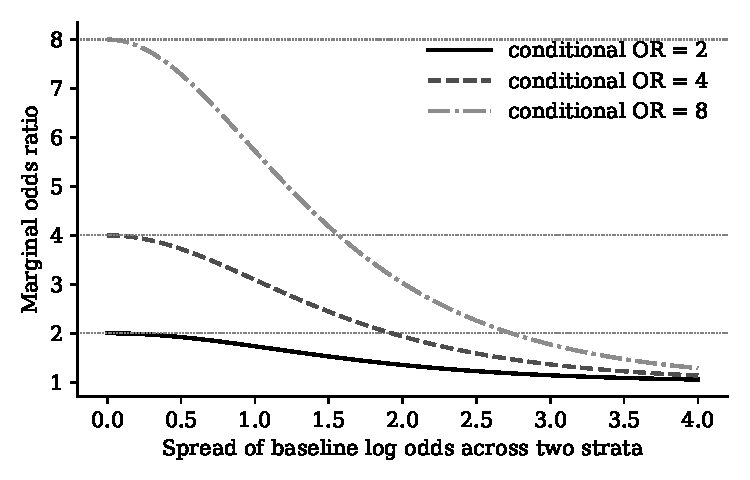
\includegraphics[width=\linewidth]{noncollapse.pdf}
\caption{Marginal odds ratio against the spread of baseline log odds in two equal strata, for three values of the common conditional odds ratio (marked by dotted lines).}
\label{fig:noncollapse}
\end{figure}

\begin{proposition}
Under randomization with the same assignment probability in every stratum, the marginal risk difference equals the $Q$ weighted average of the conditional risk differences, where $Q$ is the stratum distribution. When the conditional odds ratio is the same in every stratum and different from one, the marginal odds ratio equals it only when the baseline risk is constant across strata, and is otherwise strictly closer to one.
\end{proposition}

\begin{proof}
The marginal risks are $\bar p_t = \sum_k q_k p_{kt}$, so $\bar p_1 - \bar p_0 = \sum_k q_k(p_{k1} - p_{k0})$. For a common odds ratio $c > 1$, write $p_{k1} = g(p_{k0})$ with $g(p) = cp/\{1 + (c - 1)p\}$. Since $g$ is strictly concave and $g(p) > p$, Jensen's inequality gives $\bar p_0 < \bar p_1 \le g(\bar p_0)$, with equality on the right only when the baseline risks coincide. The increasing odds $h(p) = p/(1 - p)$ satisfy $h\{g(p)\} = c\,h(p)$, hence $1 < h(\bar p_1)/h(\bar p_0) \le c$. The case $c < 1$ follows by exchanging treatment and control. Appendix~\ref{app:theory} gives the details.
\end{proof}

The risk difference is collapsible and the odds ratio is not, which is often offered as a reason to prefer the risk difference. The model first view draws the opposite lesson: the model is logistic, its natural parameter is $\beta$, and every marginal summary, risk difference or odds ratio, is accounting. Prefer the model, and compute whatever summary the user needs. Section~\ref{gr:sec:many} makes the point exact: for one conditional odds ratio above one, the average risk difference takes every value between zero and a bound set by the odds ratio, depending on the case mix.

Pearl reaches a related conclusion in Chapter 6 of \emph{Causality} (Pearl 2009), from confounding rather than models: a change in the odds ratio on adjustment is not evidence of confounding, so collapsibility cannot serve as a test for it (Greenland, Robins and Pearl 1999). Section~\ref{fw:sec:pearlbook} reads this book alongside Pearl.

\section{Logistic regression and the choice of scale}

We use logistic regression\index{logistic regression|textbf} because the log odds\index{log odds|textbf} is the canonical parameter of the Bernoulli family, and because for some treatments the conditional odds ratio is more stable across populations than the risk difference\index{logistic regression!choice of scale|textbf}. If a treatment's conditional odds ratio is roughly constant across patients with different baseline risks, a log odds model needs fewer interactions than a risk difference model, and is therefore easier to estimate and more transportable.

Whether the odds ratio is the more stable scale depends on the treatment, but the choice illustrates a general point: the modelling scale is chosen for the model's stability and simplicity, the reporting scale for the user's needs, and they need not coincide. The model first view separates them; estimand first methods tend to conflate them by modelling directly on the reporting scale. Section~\ref{gr:sec:gap} measures how stable each scale is by an information gap, and finds the odds ratio the least stable of three for the kidney stone data of Table~\ref{fw:tab:simpson}.

\paragraph{Covariate adjustment in randomized trials.} Adjusting for a prognostic covariate changes the odds ratio even under perfect randomization (Table~\ref{tab:noncollapse}), leading critics to say that adjustment ``changes the estimand''\index{noncollapsibility}.

On the model first view, adjustment changes the model, not the estimand. The adjusted model describes the data better because it includes a predictor of the outcome. The marginal risk difference, if the regulator wants it, is computed from the adjusted model by averaging over the trial's covariate law, and in large trials, when the adjusted model is correctly specified, is at least as precise as the unadjusted difference in proportions. 

\section{Finite population and superpopulation}

Neyman's randomization analysis targets the finite population effect\index{finite population effect}\index{average treatment effect!finite population|textbf} $\tau_{\mathrm{fp}}$; most model based analyses target the superpopulation\index{superpopulation} effect\index{average treatment effect!superpopulation|textbf} $\tau$.

On the model first view the superpopulation effect is the accounting identity $\tau_Q$ with $Q$ the superpopulation covariate law. The finite population effect averages the completed table of potential outcomes, so it is a function of the observed and imputed outcomes rather than of $\theta$. A Bayesian computes both from one fit: the first from $\theta$ and, when $Q$ is known only through the sample, the Bayesian bootstrap weights above; the second from $\theta$ and draws of the missing outcomes.

The superpopulation posterior carries uncertainty about $\theta$ and $Q$, which shrinks with $n$. The finite population posterior conditions on the observed outcomes and imputes the rest; its uncertainty depends on the association between $Y(0)$ and $Y(1)$, which the data never inform. In the bivariate normal case of Chapter~\ref{ch:predictive} without covariates, $\tau$ is the difference of means and $Q$ drops out. Take flat priors on the means, known standard deviations $\sigma_0$ and $\sigma_1$, correlation $\rho$ between $Y(0)$ and $Y(1)$, and $n_1$ treated and $n_0$ control units, $n = n_1 + n_0$. The posterior variances are
\begin{align*}
\mathrm{Var}(\tau \mid \text{data}) &= \frac{\sigma_1^2}{n_1} + \frac{\sigma_0^2}{n_0}, \\
\mathrm{Var}(\tau_{\mathrm{fp}} \mid \text{data}) &= \frac{1}{n}\Bigl(\sigma_1^2\,\frac{n_0}{n_1} + \sigma_0^2\,\frac{n_1}{n_0} + 2\rho\,\sigma_0\sigma_1\Bigr),
\end{align*}
and their difference is $\mathrm{Var}\{Y(1) - Y(0)\}/n = (\sigma_1^2 + \sigma_0^2 - 2\rho\sigma_0\sigma_1)/n$, which is never negative. The finite population effect is therefore never more uncertain than the superpopulation effect, and its variance rises with $\rho$. With $n_1 = n_0 = 50$ and $\sigma_0 = \sigma_1 = 1$ the superpopulation variance is 0.040, while the finite population variance is 0.010, 0.020, 0.030 and 0.040 at $\rho = -0.5$, $0$, $0.5$ and $1$. The two variances coincide only for constant unit effects, $\rho = 1$ with equal standard deviations, when both equal Neyman's conservative variance\index{Neyman conservative variance estimator@Neyman's conservative variance estimator} $\sigma_1^2/n_1 + \sigma_0^2/n_0$. Otherwise it is an upper bound on the finite population variance, so the randomization analyst who uses it reports the interval for constant effects without assuming them. With unequal standard deviations the bound exceeds even the largest finite population variance, the one at $\rho = 1$, by $(\sigma_1 - \sigma_0)^2/n$. The Bayesian states the association explicitly, by a prior, and can show the reader how much the finite population interval depends on it.

A ministry extending a programme to next year's cohort wants the superpopulation effect under that cohort's covariate law. A court asking what the trial's participants gained wants their finite population effect. Both come from one fit; reporting both, with the association prior stated, adds one imputation step to the posterior draws.

\section{What this does to double machine learning}

DML fixes a target functional, typically the average treatment effect, then builds an estimator from an orthogonal score, so that its first order error is insensitive to errors in the nuisance functions. Part II gives the details.

On the model first view the functional is an accounting step\index{accounting identity!and double machine learning|textbf}, and DML\index{double machine learning!and accounting|textbf} concentrates on it. The hard part, getting the conditional model right, is delegated to black box learners, with orthogonalization and cross fitting keeping their errors from reaching the estimate to first order.

The Bayesian alternative reverses the emphasis: spend the effort on the model and its prior, then propagate uncertainty about the nuisance functions to every summary, rather than making it second order and leaving it out of the interval.

DML builds one estimate and interval per functional. The effect on the treated\index{effect on the treated}, a subgroup effect and a quantile effect each need a score: the first two can reuse the outcome and propensity fits, while quantiles need new nuisance fits. Joint intervals need stacked scores and their covariance. One posterior supplies all these summaries with joint uncertainty; estimates from different DML scores and splits need not cohere.

\section{The average treatment effect in econometrics}

Econometrics usually treats the average treatment effect\index{average treatment effect!in econometrics|textbf} as a fixed population parameter to be estimated consistently and efficiently. Semiparametric efficiency theory (Bickel, Klaassen, Ritov and Wellner 1993; Hahn 1998) gives the smallest asymptotic variance for a regular estimator; DML attains it when nuisance estimators converge fast enough.

The accounting view accepts that the average treatment effect is well defined, but denies that it is the natural object of inference. In survey sampling, a design based estimator targets a population mean directly; modelling the population targets the same number when the model is right, and gives much more besides.

Efficiency theory is also less decisive than it looks: the efficient estimator changes with the target. In a correctly specified regular parametric model, the Bernstein von Mises\index{Bernstein von Mises theorem} theorem makes a Bayesian posterior efficient for every smooth functional at once, provided the prior has a positive continuous density at the true parameter. The posterior attains the parametric efficiency bound for each target without being rebuilt. The semiparametric bound for the average effect is subtler: an outcome surface prior that ignores the propensity score can leave a first order bias in the functional, so a nonparametric prior attains the bound only under conditions (Appendix~\ref{app:guarantees} and Section~\ref{sec:rrw}).

\section{Objections}

\paragraph{Misspecification.} If the logistic model is wrong, its posterior functional is wrong too, whereas DML is robust to some nuisance errors\index{accounting identity!objections to|textbf}. Our reply, developed in Part III, is that a flexible model with a heavy tailed shrinkage prior is not a parametric logistic regression. The model first view does not require a small model, only a coherent probability model from which summaries are computed.

\paragraph{Counterfactual metaphysics.} Dawid (2000) objects that potential outcomes are metaphysical, since we never observe both. We half agree. Superpopulation and conditional effects can be defined without counterfactuals, through the decision theoretic contrast of interventional distributions described in Chapter~\ref{ch:predictive}. Individual attributions cannot, and neither can effects defined on the units of one sample; Part IV treats the attributions as partially identified for that reason.

\paragraph{The estimand framework.} Under the ICH E9(R1) addendum, regulators ask trial sponsors to specify the estimand before the analysis, which might seem to favour the estimand first view. The addendum asks for five attributes: the treatment, the population, the outcome variable, the handling of intercurrent events and the population level summary. In our language, the population is $Q$ and the summary is the functional; the other three fix what the model describes. None requires a separate estimator. A prespecified posterior functional of a model built on those choices satisfies the addendum (Exercise~\ref{ex:ch02:6}).

\paragraph{Computation.} DML is cheap, a handful of regressions, while posterior computation can be expensive. This is a real advantage, and Chapter~\ref{ch:computation} shows that for the horseshoe models of this book a Gibbs sampler closes most of the gap, and that where the likelihood is costly to evaluate, a map learned once from simulations (generative Bayesian computation) returns posterior draws for each new data set in a single pass.

\section{One posterior, several accountings: a worked example}

We simulate one data set of 1,500 people with standardized age $A \sim N(0,1)$\index{accounting identity}\index{accounting identity!one posterior, several accountings|textbf}. Treatment probability is $\Prob(T = 1 \mid A = a) = \expit(0.8a)$, and the outcome follows
\[
\logit\Prob(Y = 1 \mid T = t, A = a) = -0.5 + 0.8t + 0.6a - 0.7ta.
\]
The treatment helps the young and harms the old: the log odds contrast $0.8 - 0.7a$ changes sign at $a = 8/7$, and the risk difference is about 0.20 at $a = 0$ and $-0.14$ at $a = 2$. We fit the logistic model with an interaction and represent the posterior by 400 draws from a Bayesian bootstrap\index{Bayesian bootstrap} of the maximum likelihood fit, in the weighted likelihood form of Newton and Raftery (1994): each draw refits the model with the units reweighted by independent standard exponential weights, which approximates the posterior under a flat prior in large samples.

From the same draws we compute three average treatment effects on the risk difference scale: for the sample covariate law, for the treated units only, and for a hypothetical older cohort whose standardized age is normal with mean one and standard deviation one, represented by 5,000 ages drawn once from that law and used for every draw. Figure~\ref{fig:tauQ} shows the three posteriors\index{average treatment effect!posterior of}.

\begin{figure}[ht]
\centering
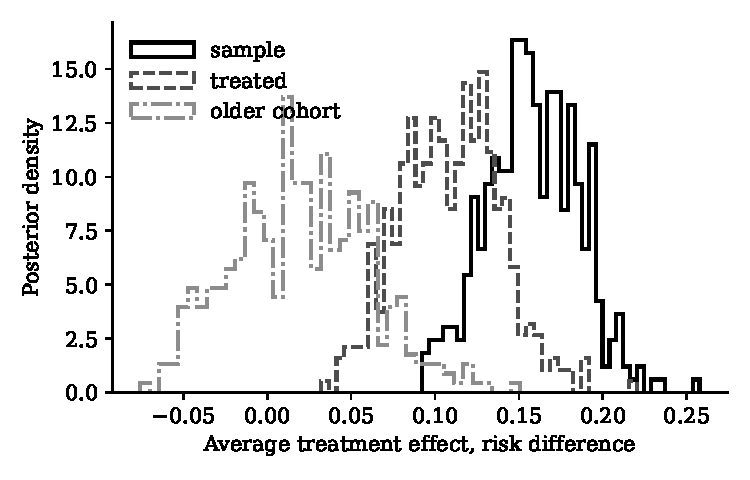
\includegraphics[width=\linewidth]{tauQ.pdf}
\caption{Posteriors of three average treatment effects computed from one logistic posterior: the sample, the treated units, and an older cohort.}
\label{fig:tauQ}
\end{figure}

The posterior means and standard deviations are 0.158 and 0.027 for the sample, 0.109 and 0.030 for the treated units, and 0.020 and 0.040 for the older cohort. The effect for the sample is clearly positive; the effect for the older cohort is indistinguishable from zero.


The numbers differ because the treated units and the older cohort are older than the sample, and treatment does less for older people. 

\section{The Lanarkshire milk experiment and randomization}\chlabel{ch:milk}\label{sec:milk}

The Lanarkshire\index{Lanarkshire milk experiment|textbf} milk experiment shows that a large trial with a poor assignment mechanism can be worth less than a small trial with a good one. Student made that case in 1931, and his argument is still the clearest account of why randomization\index{randomization|textbf} matters.

It is also where the model first view meets its limit: a model fitted to the recorded variables can remove selection on those variables and cannot remove selection on anything else, and no amount of data, 20,000 children included, tells the two apart. Randomization does not enter the likelihood; Rubin's\index{Rubin, Donald B.!ignorability|textbf} reason for a Bayesian to care is that it makes the assignment mechanism\index{assignment mechanism!and randomization|textbf} ignorable.

\subsection{The experiment}

In the spring of 1930 the Department of Health for Scotland ran a feeding trial on about 20,000 schoolchildren in 67 schools in Lanarkshire. Around 10,000 children received three quarters of a pint of milk a day for four months, from February to June. Half of those received raw milk and half pasteurized; the other 10,000 were controls. Every child was weighed and measured at the start and end, and the report by Leighton and McKinlay (1930) concluded that milk produced a definite improvement in growth.

On paper the design was careful: within each school, children were to be allocated to milk or control by ballot or by alphabet. The trouble lay in one permission. If the groups looked unbalanced, with too many well fed or ill nourished children in one, the teachers could substitute children to restore balance.

Student's reading was that the teachers, swayed by the very human feeling that poorer children needed the milk more, unconsciously substituted too many ill nourished children into the milk group and too few into the controls. Their intervention was kind and nutritionally sensible, and it made the two groups unequal at the start.

\subsection{What Student found}

Student found\index{Lanarkshire milk experiment!Student's analysis|textbf} in the report that controls began ahead of the milk group by about three months' growth in weight and four months' growth in height. Any four month growth difference therefore mixed milk's effect with differences in how smaller, poorer children grew.

A second problem was subtler. Children were weighed in their indoor clothes, and Student judged that older children wore about a pound more clothing in February than in June. Since the selection was probably related to poverty, the milk group would have shed less clothing than the controls, inflating its apparent gain in weight. This fits his observation that the estimated benefit of milk was 8 to 10 per cent of the gain in height but 30 to 45 per cent of the gain in weight, rising to over 70 per cent among older children, who had the most clothing to shed.

A third problem concerned raw against pasteurized milk. Each school received only one kind, and controls were pooled across schools. Fisher and Bartlett (1931) concluded that raw milk was superior, but conditionally: if the raw and pasteurized groups were random samples from the same population, the differences would be decisive. Student was cautious: in a socially heterogeneous district, the 67 schools, split into groups of about 33 and 34, could differ in their children's starting measurements and growth rates. Treatment assigned by school is confounded with the school, however many children it contains.

For a repeat at the same scale, Student proposed matching children on age, sex and condition, then tossing a coin within each pair to assign milk. Taking milk's benefit as agreed, he proposed twins for the raw against pasteurized comparison. Lanarkshire might have 200 to 300 pairs, about 50 identical; a coin would assign one twin raw milk and the other pasteurized. He judged that 50 pairs of identical twins would give more reliable results than the 20,000 children at a tiny fraction of the cost.

\subsection{A simulation in the spirit of Lanarkshire}

We cannot reanalyse the Lanarkshire measurements, so we simulate the mechanism\index{Lanarkshire milk experiment!simulation|textbf}\index{simulation study!Lanarkshire|textbf}. Children have a standardized initial size $S$. Without milk their four month gain is $G(0) = 1 - 0.3 S + \varepsilon$, with $S \sim N(0,1)$ and $\varepsilon \sim N(0, 0.5^2)$, so smaller children grow more, as children below their growth curve tend to. Milk adds $0.2$ to the gain. Teachers assign milk with probability $\expit(-1.2 S)$, favouring small children.

Figure~\ref{fig:milk} shows the result for 2,000 simulated children. The naive difference in mean gain between milk and control is 0.49, more than twice the true effect, because the milk group is full of small children who would have grown more anyway. A regression of gain on treatment and initial size recovers 0.22, as does a properly randomized trial on the same population, in which a fair coin reassigns the same 2,000 children.

\begin{figure}[ht]
\centering
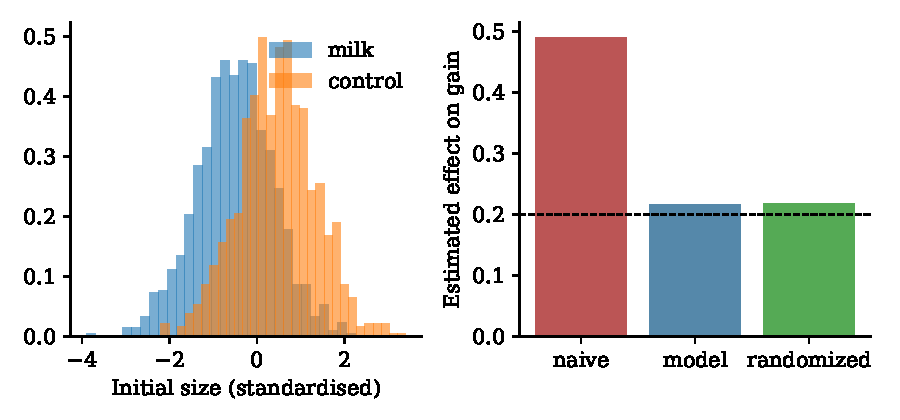
\includegraphics[width=\linewidth]{milk_sim.pdf}
\caption{Simulated milk trial. Left: initial size in the two groups after teacher substitution. Right: naive, model based and randomized estimates; the dashed line is the true effect of 0.2.}
\label{fig:milk}
\end{figure}

The model works because teachers selected on recorded $S$ alone.

Suppose instead that the teachers went by how well nourished a child looked, a score $U$ that nobody wrote down, and that recorded size is only a proxy for it: $(S, U)$ is standard bivariate normal with correlation $r$. Milk goes to a child with probability $\expit(-1.2\,U)$, the rule above with $U$ in place of $S$, and the gain is $1 - 0.3S - 0.3U + 0.2T + \varepsilon$, so a child who looks poorly nourished grows more whatever its size. Over 1,000 simulated trials of 2,000 children, the regression of gain on treatment and size puts the effect of 0.2 at 0.23 on average when $r = 0.95$, at 0.32 when $r = 0.8$ and at 0.42 when $r = 0.5$; when size says nothing about nourishment it gives 0.48, no better than the naive comparison (Monte Carlo standard errors about 0.001; Exercise~\ref{ex:ch03:2} derives these values). A record that correlates 0.8 with what the teachers saw still leaves a bias of 0.12, more than two fifths of the 0.28 left when size says nothing about nourishment. The Lanarkshire teachers looked at the children; the records hold their height, weight, age, sex and school.

\subsection{Randomization in Bayesian terms}

Rubin (1978) made precise what randomization\index{randomization!in Bayesian terms|textbf} buys a Bayesian. Write the full data as covariates $X$, potential outcomes $Y(0), Y(1)$ and assignments $T$. Let $Y_{\mathrm{obs}}$ contain outcomes under the assigned arms and $Y_{\mathrm{mis}}$ those under the other arms. The assignment mechanism\index{assignment mechanism} is
\[
p(T \mid X, Y(0), Y(1), \phi).
\]

\begin{definition}[Ignorable assignment]
The assignment mechanism is ignorable if
\[
p(T \mid X, Y(0), Y(1), \phi) = p(T \mid X, Y_{\mathrm{obs}}, \phi)
\]
and $\phi$ is a priori independent of the parameter $\theta$ of the outcome model. This is Rubin's version: strong ignorability (Definition~\ref{def:ignorability}) implies the first condition, which also allows assignment to depend on observed outcomes, and the second is a further requirement on the prior.
\end{definition}

\begin{theorem}[Rubin]
Under ignorable assignment, the posterior distribution of $\theta$, and of any missing potential outcomes, does not depend on the assignment mechanism.
\end{theorem}

\begin{proof}
Ignorability removes $Y_{\mathrm{mis}}$ from the assignment factor; prior independence lets $\phi$ be integrated out separately:
\begin{align*}
\pi(\theta, Y_{\mathrm{mis}} \mid X, Y_{\mathrm{obs}}, T) &\propto \pi(\theta)\, p(X, Y(0), Y(1) \mid \theta) \\
&\qquad \times \int p(T \mid X, Y_{\mathrm{obs}}, \phi)\, \pi(\phi)\, d\phi.
\end{align*}
The integral is constant in $\theta$ and $Y_{\mathrm{mis}}$, so it drops out. Integrating out $Y_{\mathrm{mis}}$ gives the posterior of $\theta$.
\end{proof}

Randomization guarantees ignorability\index{ignorability} by design, because a random number generator does not look at the potential outcomes. This is the precise sense in which randomization matters to a Bayesian: without it the outcome model must also model the teachers. Selection on recorded variables is ignorable conditional on them. The Lanarkshire teachers also went by apparent nourishment; if that unrecorded information predicted growth, the analysis must model the teachers or report its sensitivity to them.

\paragraph{Randomization and the likelihood principle.} The likelihood principle\index{likelihood principle|textbf} says inference should depend on the data only through the likelihood, and the randomization distribution is not part of it. Randomization does not change the likelihood of the observed data under a correct model; it makes the correct model easier to write down, and so insures against the analyst's ignorance of the selection process.

Kadane and Seidenfeld (1990) argue that randomization protects the experimenter\index{randomization!protects the experimenter|textbf} against others' suspicion: she may trust that her allocation was unrelated to outcomes, but her reader cannot unless she randomized.

\subsection{What a model based reanalysis would look like}

If substitutions depended only on recorded height, weight, age, sex and school, assignment would be ignorable conditional on them. A Bayesian reanalysis\index{Lanarkshire milk experiment!model based reanalysis|textbf} would model four month weight and height gains jointly as functions of those variables, with treatment interacting with initial size. School effects would be exchangeable (partial exchangeability\index{exchangeability}). The model would absorb the initial imbalance rather than correct it by weighting.

The clothing problem would enter as measurement error: recorded weight is true weight plus clothing, whose seasonal component varies with poverty. A Bayesian measurement error model would put a prior on the February to June clothing difference, perhaps informed by the fraction of children recorded as poor, and propagate it.

The weak point is what was not recorded: teachers also judged poverty and family circumstance by eye, confounders we cannot see. The honest report is a sensitivity analysis\index{sensitivity analysis} as in Section~\ref{sec:sensitivity}, showing how strong that unrecorded selection would need to be to explain away the benefit of milk.

\subsection{Student, Guinness and small samples}

William Sealy Gosset\index{Gosset, William Sealy|textbf} published as Student\index{Student|see{Gosset, William Sealy}} because the Guinness brewery did not want competitors to know that it employed scientists. His 1908 paper introducing the $t$ distribution\index{Gosset, William Sealy!t distribution|textbf} was motivated by experiments on barley and hops with a handful of observations each. He spent his scientific life extracting reliable conclusions from small, carefully designed comparisons.

To a man used to drawing firm conclusions from a dozen paired plots, Lanarkshire\index{Lanarkshire milk experiment}, a study of 20,000 children that could not answer its question, looked wasteful. 

Gosset favoured systematic, balanced plots, including his half drill strip method, believing they controlled fertility gradients better than random allocation. Fisher insisted on randomization\index{Fisher, Ronald A.!randomization} as the only basis for a valid error estimate. Lanarkshire's failed balancing supported Fisher, and Gosset recognized it: for a repeat he recommended coin tosses within matched pairs, or at least drawing lots rather than alphabetical allocation.

\subsection{Pairing and the variance of a comparison}

Let $Y_{j1}$ and $Y_{j2}$ be the growths of the two members of pair $j$, one given milk\index{Lanarkshire milk experiment!pairing|textbf}. If each child's growth has variance $\sigma^2$ and the within pair correlation is $\rho$, the variance of the paired difference\index{pairing|textbf} is $2\sigma^2(1 - \rho)$. With $m$ pairs the estimator of the effect has variance $2\sigma^2(1-\rho)/m$. An unpaired, perfectly randomized trial with $N$ children split equally has variance $4\sigma^2/N$.

Student's claim concerned raw against pasteurized milk in the flawed trial. Figure~\ref{fig:twins} instead compares 50 twin pairs with 20,000 perfectly randomized, unpaired children; for the actual 10,000 fed children, 50 pairs break even at $\rho\approx0.99$. Against 20,000, they break even only at $\rho \approx 0.995$. Student's claim therefore depended on imperfect randomization, whose bias does not shrink with $N$. With bias $b$ in the large trial, 50 pairs have lower mean squared error when $b^2 > 2\sigma^2(1 - \rho)/50 - 4\sigma^2/N$; at $\rho = 0.9$ and $\sigma^2 = 1$, a bias of about 0.06 standard deviations is enough.

\begin{figure}[ht]
\centering
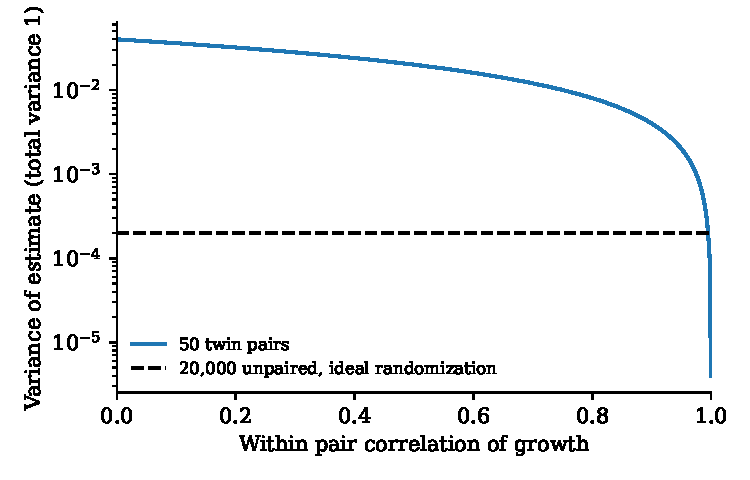
\includegraphics[width=\linewidth]{twins.pdf}
\caption{Variance of the estimated effect for 50 twin pairs, as a function of the within pair correlation of growth, against 20,000 unpaired children under ideal randomization. Total variance of growth is one. The curves meet at a correlation of 0.995, and the paired variance falls to zero at a correlation of one.}
\label{fig:twins}
\end{figure}



\paragraph{A Bayesian model for the paired design.} For twin pairs the natural model has a pair effect:
\[
Y_{jk} = \mu + \alpha_j + \tau T_{jk} + \varepsilon_{jk}, \qquad \alpha_j \sim N(0, \sigma_\alpha^2), \qquad \varepsilon_{jk} \sim N(0, \sigma_\varepsilon^2).
\]
With the variance components known and flat priors on $\mu$ and $\tau$, let $D_j$ be the treated child's growth minus the control child's in pair $j$. The pair effect cancels, so the $D_j$ are independent $N(\tau, 2\sigma_\varepsilon^2)$, and the pair averages, which are independent of the differences, inform only $\mu + \tau/2$, which the flat prior on $\mu$ leaves free. With $\bar D$ the mean difference,
\[
\tau \mid \text{data} \sim N\bigl(\bar D, 2\sigma_\varepsilon^2/m\bigr),
\]
where $\sigma_\varepsilon^2 = \sigma^2(1 - \rho)$ is the within pair residual variance, so the posterior variance is the paired variance above and $\sigma_\alpha^2$ drops out. Randomization within pairs makes the assignment ignorable conditional on the pair, so the theory of this section applies directly. Section~\ref{gr:sec:transform} adds that the coin toss within pairs makes the assignment mechanism ancillary, whatever the teachers saw.

A hierarchical extension, $\tau_j \sim N(\tau, \sigma_\tau^2)$, allows effects to vary across pairs. If $\tau_j$ is independent of $\alpha_j$, the milk and control children's growth variances differ by $\sigma_\tau^2$, so the data say how much effects vary between families; if they are correlated, $\sigma_\tau^2$ is not identified.

\subsection{Randomization inference and Bayesian inference}

Fisher's randomization test\index{randomization inference|textbf}\index{randomization test} treats potential outcomes as fixed and assignment as random. Under the sharp null of no effect on any child, growth is unchanged by assignment, so the distribution of any test statistic over all possible assignments can be computed exactly. The $p$ value is the probability, under the assignment mechanism, of a statistic at least as extreme as observed. With fair coins in $m$ pairs, it is the fraction of the $2^m$ equally likely assignments meeting that condition.

The Bayesian analysis treats the assignment as fixed, once observed, and the outcomes as random. The randomization test asks whether the observed difference is surprising under the sharp null; the posterior asks what the effect is likely to be, given the data and a model.

Both need information about the assignment mechanism: randomization inference needs each assignment's probability, and Bayesian inference can omit the mechanism only if it is ignorable. Lanarkshire's unrecorded substitution rule left the probabilities unknown and used outcome predictors. Unless the recorded measurements capture everything the teachers saw, a Bayesian must model the teachers or report sensitivity to them.

\subsection{What modern trials learned from Lanarkshire}

Several features of modern trial practice\index{randomization!what modern trials learned|textbf} can be read as answers to Student.

\paragraph{Concealed allocation.} The person enrolling a patient must not know the next assignment, or, as at Lanarkshire, can steer patients toward or away from treatment.

\paragraph{Stratified and blocked randomization.} Balance on important prognostic variables is achieved by randomizing within strata, not by substitution after randomization.

\paragraph{Prespecified analysis.} The analysis model, including covariate adjustment, is fixed before the data are seen. In the Bayesian version the prior and model are fixed, and the posterior is reported regardless of what it shows.

\paragraph{Cluster randomization.} When spillovers between units are likely, whole schools or villages are randomized. Lanarkshire allocated within schools, allowing spillovers between milk and control children in the same school.




\subsection{Lessons for the rest of the book}

Twenty thousand children selected by kind teachers told us less, in Student's judgement, than fifty pairs of identical twins would have\index{Lanarkshire milk experiment!lessons for the book|textbf}. Today's analogue is the administrative database with millions of records and an unknown selection process, whose size invites confidence its design does not justify. Many modern selection processes, from clinicians choosing treatments to algorithms targeting interventions, share the teachers' logic: the people most in need are chosen, and need predicts outcome.

Pairing and stratification are prior information about where variability lies: Student's twins encode the judgement that genetic and household differences dominate the variance of growth. A model is the natural tool for such information, because it states what was matched and what was not.

\section{In practice}

\paragraph{The target.} The target is $\tau_Q$ from \eqref{eq:tauQ}, computed draw by draw for every $Q$ of interest. For Lanarkshire the target is the expected four month gain in weight and height from milk for a child of given initial size, age and sex. Each posterior draw of the growth model gives that conditional gain; averaging over the Lanarkshire covariate distribution gives the Department's population figure, and averaging over poor children gives the figure a targeted policy needs.

\paragraph{What the analyst does differently.} The analyst states the model and the accounting separately. The model is the logistic regression \eqref{eq:logistic}, with whatever interactions the policy question needs, on the scale where the effect is most nearly stable, and it is checked as a model, by posterior predictive checks of fitted probabilities against observed frequencies. The accounting is a list of laws $Q$, each tied to a question. In the worked example (Figure~\ref{fig:tauQ}) the sample, the treated units and the older cohort gave three different posterior means on the risk difference scale, the last indistinguishable from zero; the report names all three and says which decision each serves.



The analyst records how treatment was assigned. When she controls the design, she randomizes within pairs or strata where prognostic variables are known. Otherwise she conditions on the recorded variables the assigners could have used and reports sensitivity (Section~\ref{sec:sensitivity}) to what they saw but did not record.

\paragraph{Against DML.} If the average effect is the only number wanted and the model is a low dimensional logistic regression, DML is adequate and costs less than posterior computation. The worked example shows what it leaves out: the effect on the treated and the effect for the older cohort each need a new score, while the posterior gives all three jointly. A conditional odds ratio of 4 and a marginal odds ratio of 3.45 (Table~\ref{tab:noncollapse}) are two accountings of one model, and two estimators built for two scales cannot say so. DML can no more repair a compromised design than the posterior can: its score presumes ignorability given the recorded covariates, the assumption the Lanarkshire teachers broke. The honest limit is misspecification: a wrong logistic model gives a wrong $\tau_Q$ for every $Q$, while DML's orthogonality protects it from some nuisance errors. Part III answers with a flexible model under a shrinkage prior, propensity aware where selection matters, rather than by abandoning the model.

\section*{Notes}

For noncollapsibility with covariates omitted from a randomized experiment, see Gail, Wieand and Piantadosi (1984). The estimand framework for trials is ICH (2019). Ray and van der Vaart (2020) prove a semiparametric Bernstein von Mises theorem for the mean of a binary outcome in one treatment arm, and the first order bias that a prior ignoring the propensity score can leave is the regularization induced confounding of Hahn, Carvalho, Puelz and He (2018).

Fisher (1935) is where the randomization test is set out, and Cox (1958) treats blocking and randomization from the experimenter's side. The randomization analysis of the finite population effect that the chapter sets beside the Bayesian one is Neyman (1923), given in full by Imbens and Rubin (2015).

For Lanarkshire, Leighton and McKinlay (1930) is the report, Student (1931) the critique with the proposals of pairs and twins, and Fisher and Bartlett (1931) the note on raw against pasteurized milk. Student (1908) is the paper on the $t$ distribution, and Student (1938) argues for balanced layouts in field experiments, the position that the chapter sets against Fisher's. Senn (2023) is a modern account of Student and the milk experiment. Spillovers between children in one school, which cluster randomization is meant to avoid, are modelled in Section~\ref{sec:interference}.

\begin{exercises}
\item\label{ex:ch02:1} Verify the entries of Table~\ref{tab:noncollapse}, and find stratum probabilities with a common conditional odds ratio of 4 for which the marginal odds ratio is below 2.
\item\label{ex:ch02:2} Show that the hazard ratio in a proportional hazards model is noncollapsible, and give a two stratum example with no confounding.
\item\label{ex:ch02:3} In model \eqref{eq:logistic}, derive the posterior mean and variance of $\tau_Q$ by the delta method, linearizing $\tau_Q$ about the posterior mean of $\theta$.
\item\label{ex:ch02:4} The first coherence requirement fails for a model in which $Y_{ij} = \mu + b_i + e_{ij}$ with $b_i \sim N(0, \sigma_b^2 / m_i)$ and $e_{ij} \sim N(0, \sigma_e^2)$ independent, where $m_i$ is the number of units of cluster $i$ in the sample. Explain why, and propose a coherent alternative.
\item\label{ex:ch02:5} Suppose two analysts report $\tau_Q$ for the sample's covariate law and for a population covariate law from the same logistic posterior. Add an interaction $t\,\delta^\top x$ to the logistic model and show that their posterior means can then have opposite signs.
\item\label{ex:ch02:6} Write the ICH E9(R1) estimand for a trial of milk supplementation in terms of a law $Q$ and a functional of $\theta$.

\item\label{ex:ch03:1} In the simulation of Figure~\ref{fig:milk}, derive the bias of the naive difference in means as a function of the selection slope and the growth slope, and check it against the simulated value.
\item\label{ex:ch03:2} Suppose the gain is $G = 1 - 0.3S + cU + 0.2T + \varepsilon$, where $(S, U)$ is standard bivariate normal with correlation $r$, and teachers assign milk with probability $\expit(-1.2\,U)$, the rule of the simulation but using the unrecorded $U$ alone. Derive, as a function of $r$, the bias of the coefficient of $T$ in the regression of $G$ on $T$ and $S$, and evaluate it for $c = -0.3$ and the values of $r$ simulated in Section~\ref{sec:milk}.
\item\label{ex:ch03:3} Student argued that 50 pairs of identical twins would compare raw and pasteurized milk more reliably than the 20,000 children. Take the generic comparison of Figure~\ref{fig:twins}, with all 20,000 children unpaired and perfectly randomized, and, under a model in which twin pairs share a random effect with variance $\sigma_\alpha^2$ and children have residual variance $\sigma_\varepsilon^2$, find the ratio $\sigma_\alpha^2/\sigma_\varepsilon^2$ at which his claim holds for estimating the mean effect.
\item\label{ex:ch03:4} Write a Bayesian measurement error model for the clothing problem, with clothing weight depending on season and poverty, so that poor children shed less clothing between February and June, and show how it biases the naive weight gain comparison.
\item\label{ex:ch03:5} Show that Fisher's randomization test of the sharp null of no effect is exact under complete randomization, and explain why it ceases to be exact under the Lanarkshire substitution rule.
\item\label{ex:ch03:6} Kadane and Seidenfeld (1990) argue that randomization protects the experimenter against suspicion. Formalize this as a game between an experimenter and a sceptical reader.
\end{exercises}

\chapter{Groups, Urns and Information}\label{ch:groups}

\begin{tcolorbox}[colback=gray!6,colframe=gray!50,title=In brief,fonttitle=\normalfont\itshape,coltitle=black,colbacktitle=gray!15,boxrule=0.4pt,arc=1pt]
A treatment effect that is stable across populations is a group element, and an average describes the case mix: one odds ratio of $e$ supports average effects from 0.076 to 0.232 over six case mixes. A randomized experiment is an urn from which about half the units are drawn, so the finite and infinite views of exchangeability disagree. When the units are sampled from a population, the experiment identifies only the two arm laws: the average effect is a function of them, while the fraction helped lies in a Fr\'echet interval that more data do not narrow. An information gap in nats measures the distance of the data from stability on a scale, and the posterior odds of one scale against another move at the exponential rate given by the difference of their gaps. In the kidney stone data the risk ratio is the most stable scale and the odds ratio the least, by a factor of 64 in gap. A right Haar prior gives exact coverage in a transformation model with known baselines; estimating the baseline under BART or a horseshoe loses that guarantee.
\end{tcolorbox}

Chapter~\ref{ch:mccullagh} left two questions open: which scale makes an effect stable, and how much an experiment can reveal about the association between a unit's potential outcomes.



\section{The treatment effect as a group action}\label{gr:sec:group}

For McCullagh a statistical model is a stochastic process: a probability distribution on the outcome space, indexed by the covariate and design information held fixed, from which sampling distributions, expectations and the properties of summaries follow. We call this the process view. The von Mises programme\index{Mises, Richard von@von Mises, Richard!frequency definition of probability|textbf} runs the other way, defining probability as a limiting relative frequency, and in McCullagh's reading potential outcomes inference inherits that definition and adds random sampling from a population. The frequency view suits concrete populations, finite and open to simple random sampling, as in surveys and auditing. In science the population is abstract, infinite and only partly accessible, and there is no sampling frame. 

McCullagh formalizes treatment assignment as a Markov kernel from covariates and an auxiliary randomization device to the treatment vector, the mechanism $p(T\mid X,Y(0),Y(1),\phi)$ of Chapter~\ref{ch:mccullagh}. In a randomized design the kernel depends only on covariates and a device with known law. It contains no outcome model parameter, so treatment is ancillary\index{ancillarity|textbf} for those parameters and Rubin's factorization follows. In a flawed experiment or observational study the kernel can depend on quantities outside the model. Dawid (2000) reaches the same place by decision theory (Section~\ref{fw:sec:dawid}). With $F_{x,t}$ the response law at covariate $x$ under treatment $t$, a group element and a posterior functional (Chapter~\ref{ch:predictive}) index the same intervention laws $(F_{x,0},F_{x,1})$.

McCullagh defines the effect of a treatment as a group element. Let $\{P_\gamma:\gamma\in\mathcal C\}$ be the laws of the response under control, with $\gamma_i=\gamma(x_i)$ the baseline of unit $i$, and let a group $G$ act on the baseline space $\mathcal C$.

\begin{definition}[Model based treatment effect]\label{gr:def:effect}\index{group action!treatment effect as|textbf}
Assume that $G$ acts freely on $\mathcal C$ and that $\gamma\mapsto P_\gamma$ is one to one. Level $t$ of the treatment corresponds to an element $g_t\in G$ with $g_0=1_G$, and a unit with baseline $\gamma_i$ given level $t$ has law $P_{g_t\gamma_i}$. The effect of level $t$ is $g_t$, common to all units. Only the baseline varies.
\end{definition}



\begin{table}[ht]
\centering
\caption{Four groups acting on a baseline. In each row $\psi$ is the effect on the scale in which the group acts by translation.}
\label{gr:tab:groups}
\begin{tabular}{@{}lll@{}}
\toprule
baseline space $\mathcal C$ & action & model \\
\midrule
$\R$ (mean) & $\gamma\mapsto\gamma+\psi$ & linear, additive effect \\
$(0,\infty)$ (rate) & $\gamma\mapsto e^{\psi}\gamma$ & log linear, rate ratio $e^{\psi}$ \\
$\R$ (log odds) & $\gamma\mapsto\gamma+\psi$ & logistic, odds ratio $e^{\psi}$ \\
$(0,\infty)$ (hazard) & $\gamma\mapsto e^{\psi}\gamma$ & proportional hazards, hazard ratio $e^{\psi}$ \\
\bottomrule
\end{tabular}
\end{table}

The point is stability: $g_t$ means the same thing for every covariate configuration and every subset of units. For the additive group of the line, write $\psi$ for the effect and keep $\tau$ for averages. In the logit row of Table~\ref{gr:tab:groups}, translation of the log odds by $\psi$ gives the risk map $g(p)=e^{\psi}p/\{1+(e^{\psi}-1)p\}$ of Chapter~\ref{ch:mccullagh}. Here $\psi$ is the conditional log odds ratio, the $\beta$ of equation~\eqref{eq:logistic}; the baseline log odds $\gamma$ is not that equation's coefficient vector $\gamma$.

The potential outcomes tradition defines the effect differently, as the Neyman and Rubin average $\tau_{\mathrm{fp}}=n^{-1}\sum_i\{Y_i(1)-Y_i(0)\}$ of Chapter~\ref{ch:predictive}, or its population analogue. With both potential outcomes observed, Battey and Edgar (2026) state that the two agree for every sample exactly when (C1) the treatment acts through the baseline parameter, (C2) the same action can be written on the observations, and (C3) no further nuisance parameter enters. They note that C1 and C2 make the model a transformation family\index{transformation model|textbf}. The linear and exponential models satisfy the conditions, the Weibull only in part, and the additive rate and logistic models fail, so that for them $\tau_{\mathrm{fp}}$ depends on the sample on every scale. The agreement is on the scale in which the group acts by translation. In the exponential model with rate ratio $e^{\psi}$, the comonotone coupling gives $Y_i(1)=e^{-\psi}Y_i(0)$, so the raw difference is $(e^{-\psi}-1)$ times the mean control outcome, which changes with the sample, while the difference of log outcomes is the constant $-\psi$.



\begin{lemma}[Translation chart]\label{gr:lem:chart}
Let $G$ be a connected one dimensional Lie group acting continuously, freely and transitively on an open interval $I\subset\R$. Then $G$ is isomorphic to $(\R,+)$, and there are an increasing homeomorphism $h:I\to\R$, the chart, and an isomorphism $\psi:G\to\R$ with
\[
h(gy)=h(y)+\psi(g)\qquad\text{for all } g\in G,\ y\in I.
\]
\end{lemma}

The proof is in Appendix~\ref{app:groupsproofs}. The logit group on the interval $(0,1)$ of risks has $h=\logit$ and $\psi(g)$ the log odds ratio.

\section{One stable effect, many averages}\label{gr:sec:many}

Take $\logit\Prob(Y_i=1)=\gamma_i+\psi t_i$, with $t_i\in\{0,1\}$ and $\psi=1$, a conditional odds ratio of $e\approx2.72$ for every unit. The baseline log odds have law $Q=N(\mu,s^2)$, the image of the covariate law under $x\mapsto\gamma(x)$; later sections use $Q$ for the covariate law itself. The average effect for this case mix\index{case mix|textbf} is the accounting identity of Chapter~\ref{ch:mccullagh}
\begin{equation}
\tau_Q(\psi)=\E_Q\{\expit(\gamma+\psi)-\expit(\gamma)\}.
\label{gr:eq:tauQ}
\end{equation}
Table~\ref{gr:tab:tau} and Figure~\ref{gr:fig:tau} give its values by Monte Carlo, with 400,000 draws of $\gamma$ for each row and each point.

\begin{table}[ht]
\centering
\caption{One conditional odds ratio, $e$ in every row, and six case mixes: the baseline log odds is $N(\mu,s^2)$ and $\psi=1$. The control risk $\E_Q\expit(\gamma)$ and the average effect $\tau_Q$ are Monte Carlo averages over 400,000 draws of the baseline (seed 1), with standard errors below 0.001, and the marginal odds ratio is computed from the two marginal risks.}
\label{gr:tab:tau}
\begin{tabular}{@{}cccccc@{}}
\toprule
$\mu$ & $s$ & control risk & $\tau_Q$ & conditional odds ratio & marginal odds ratio \\
\midrule
$-3.0$ & 0.5 & 0.053 & 0.076 & 2.72 & 2.66 \\
$-2.0$ & 0.5 & 0.129 & 0.150 & 2.72 & 2.62 \\
$-0.5$ & 0.5 & 0.384 & 0.232 & 2.72 & 2.57 \\
$-0.5$ & 2.0 & 0.424 & 0.151 & 2.72 & 1.84 \\
$-0.5$ & 3.0 & 0.442 & 0.115 & 2.72 & 1.59 \\
$\phantom{-}2.0$ & 0.5 & 0.871 & 0.076 & 2.72 & 2.66 \\
\bottomrule
\end{tabular}
\end{table}

\begin{figure}[ht]
\centering
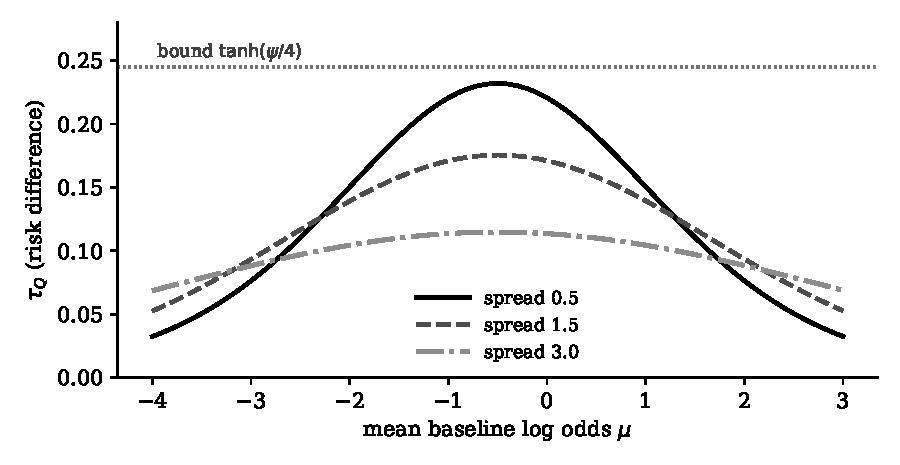
\includegraphics[width=\linewidth]{tau_case_mix.pdf}
\caption{The average effect $\tau_Q$ against the mean baseline log odds $\mu$, for baseline spreads $s=0.5$ (solid line), $1.5$ (dashed line) and $3.0$ (dash and dot line), with $\psi=1$ so that the conditional odds ratio is $e$ throughout. Each curve is a Monte Carlo average over the same 400,000 draws of a standard normal, at 71 values of $\mu$ from $-4$ to $3$. The dotted horizontal line is the bound $\tanh(\psi/4)=0.245$ of Proposition~\ref{gr:prop:range}.}
\label{gr:fig:tau}
\end{figure}

The conditional odds ratio is $e$ in every row, yet the average effect ranges over a factor of three, from $0.076$ to $0.232$. Spread alone, with $\mu=-0.5$ fixed, takes it from $0.232$ to $0.115$. The marginal odds ratio is below $e$ in every row and falls to $1.59$ at $s=3$, the noncollapsibility of Chapter~\ref{ch:mccullagh}. Each curve in Figure~\ref{gr:fig:tau} peaks at $\mu=-\psi/2$, where the control and treated risks lie symmetrically about one half, and the peak falls as the spread grows. 

\begin{proposition}\label{gr:prop:range}
Fix $\psi>0$ and let $Q$ range over all probability laws for the baseline log odds $\gamma$ in \eqref{gr:eq:tauQ}. Then
\[
\{\tau_Q(\psi):Q\}=\bigl(0,\ \tanh(\psi/4)\bigr],
\]
with the supremum attained only by the point mass at $\gamma=-\psi/2$. Equivalently, an average effect $\tau\in(0,1)$ is generated by the odds ratio $e^{\psi}$ under some case mix if and only if $\psi\ge4\operatorname{artanh}(\tau)$.
\end{proposition}

Since $\expit'$ is even and decreases away from zero, $d(\gamma)=\expit(\gamma+\psi)-\expit(\gamma)$ increases up to $\gamma=-\psi/2$ and decreases thereafter, so $\tau_Q(\psi)\le d(-\psi/2)=\tanh(\psi/4)$ (full proof in Appendix~\ref{app:groupsproofs}). At $\psi=1$ this is $0.245$, the dotted line in Figure~\ref{gr:fig:tau}. Without the baseline distribution, then, $\tau_Q$ bounds $\psi$ only from below and $\psi$ bounds $\tau_Q$ only from above. An average effect of $0.232$ needs $\psi\ge0.945$, an odds ratio of at least $2.57$, while $0.076$ needs only $\psi\ge0.305$, an odds ratio of at least $1.36$. Two populations that differ only in case mix report $0.076$ and $0.232$ for the same treatment. This is McCullagh's critique in numbers: $\tau_Q$ describes the case mix, $\psi$ describes the treatment.

\section{A randomized experiment is an urn}\label{gr:sec:urn}

The urn form of de Finetti's theorem, due to Heath and Sudderth (1976), shows where the gap between the finite population and superpopulation posteriors of Chapter~\ref{ch:mccullagh} comes from.

\begin{theorem}[Heath and Sudderth]\label{gr:thm:hs}
Let $Z_1,\dots,Z_n$ be exchangeable with values in $\{0,1\}$ and let $S=\sum_iZ_i$. Given $S=r$, the sequence is distributed as $n$ draws without replacement from an urn\index{Heath and Sudderth urn|textbf}\index{urn|see{Heath and Sudderth urn}} with $r$ ones and $n-r$ zeros. Hence for $k\le n$ and $s=\sum_{i\le k}z_i$,
\[
\Prob(Z_1=z_1,\dots,Z_k=z_k)=\sum_{r=0}^n \Prob(S=r)\,\frac{(r)_{s}\,(n-r)_{k-s}}{(n)_k},
\]
with $(a)_j=a(a-1)\cdots(a-j+1)$. If the sequence extends to an infinite exchangeable sequence, $S/n$ converges in law to a limit with law $\Pi$ as $n\to\infty$, and the display becomes de Finetti's theorem, $\Prob(Z_{1:k}=z_{1:k})=\int\theta^{s}(1-\theta)^{k-s}\,\Pi(d\theta)$.
\end{theorem}

\begin{proof}
Given $S=r$ every arrangement of $r$ ones among $n$ places is equally likely, which is the urn, and the display is the probability that the first $k$ draws show $z_{1:k}$. As $n\to\infty$, $(r)_s(n-r)_{k-s}/(n)_k-(r/n)^s(1-r/n)^{k-s}\to0$ uniformly in $r$, and the laws of $S/n$ converge, because $\E\{(S)_j/(n)_j\}=\Prob(Z_1=\dots=Z_j=1)$ for every $n\ge j$ and $(S)_j/(n)_j-(S/n)^j\to0$ uniformly, so the moments of $S/n$ converge and determine the limit on $[0,1]$.
\end{proof}

The rate is explicit. Diaconis and Freedman (1980) show that the first $k$ of $n$ exchangeable variables taking $c$ values are within $ck/n$ in total variation of a mixture of independent and identically distributed laws\index{de Finetti theorem@de Finetti's theorem!finite version}, and within $k(k-1)/(2n)$ whatever the number of values. (Their norm is twice this distance, so Appendix~\ref{app:theory} states $2ck/n$.) Figure~\ref{gr:fig:hs} shows the exact distance for an urn half full: about $k/(4n)$ for small $k$ and 0.16 to 0.17 at $k=n/2$, whatever $n$. For this urn the finite and infinite views agree only when $k/n$ is small, and at $k=n/2$ the bound says nothing.

\begin{figure}[ht]
\centering
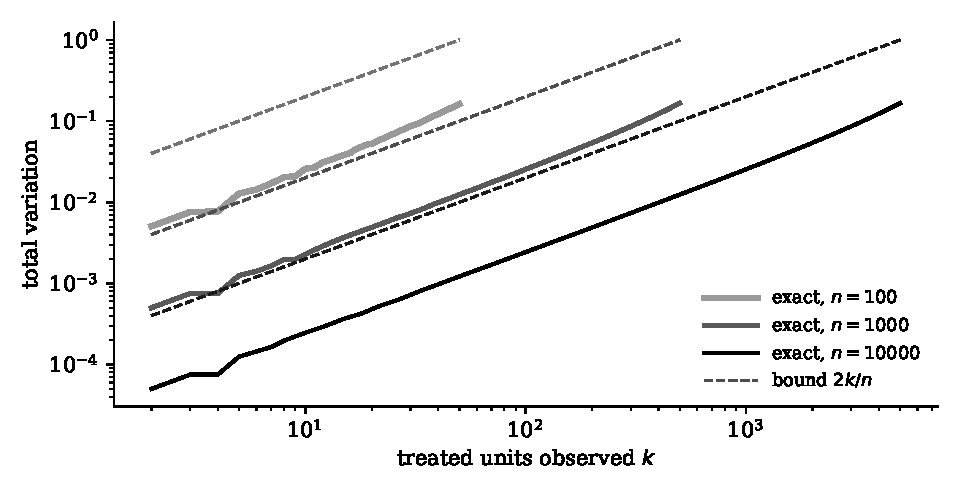
\includegraphics[width=\linewidth]{heath_sudderth_tv.pdf}
\caption{Total variation distance between $k$ draws without replacement from an urn of $n$ units, half of them ones, and $k$ independent draws with probability one half, against $k$ on logarithmic scales, for $n=100$ (thick light line), $1{,}000$ (medium dark line) and $10{,}000$ (thin black line). Exact hypergeometric and binomial calculations at up to 40 log spaced values of $k$ from 2 to $n/2$. Thin dashed lines: the bound $ck/n=2k/n$ of Diaconis and Freedman, capped at 1; the distance is less than one sixth of it.}
\label{gr:fig:hs}
\end{figure}

Fix $n$ units with potential outcomes $(Y_i(1),Y_i(0))$. Complete randomization\index{randomization!as an urn|textbf} draws $n_1$ units uniformly without replacement: treated responses are draws from $\{Y_i(1)\}$ and controls are complementary draws from $\{Y_i(0)\}$. Neyman's randomization inference fixes the unknown urn composition, a degenerate mixing measure, and puts probability only on assignment.

\begin{proposition}\label{gr:prop:fpc}
Let $p_1$ be the proportion of ones in a binary urn $\{Y_i(1)\}$ and $\bar Y_1$ the mean of the $n_1$ treated responses. Under complete randomization
\[
\mathrm{Var}(\bar Y_1)=\frac{p_1(1-p_1)}{n_1}\cdot\frac{n-n_1}{n-1},
\]
so the urn differs from the de Finetti limit by the finite population correction\index{finite population correction|textbf} $(n-n_1)/(n-1)$. For outcomes of any kind and the difference in means $\hat\tau=\bar Y_1-\bar Y_0$, Neyman's variance is
\[
\mathrm{Var}(\hat\tau)=\frac{S_1^2}{n_1}+\frac{S_0^2}{n_0}-\frac{S_\tau^2}{n},
\]
where $S_1^2$, $S_0^2$ and $S_\tau^2$ are the finite population variances, with divisor $n-1$, of $Y(1)$, $Y(0)$ and the unit effects $\tau_i$. If the additive group of Section~\ref{gr:sec:group} also acts on the observations unit by unit, $Y_i(1)=Y_i(0)+\psi$ for all $i$ (condition C2 of Battey and Edgar, 2026, with its deterministic coupling, which by Lemma~\ref{gr:lem:binary} binary outcomes satisfy only trivially), then $S_\tau^2=0$ and Neyman's conservative variance estimator is unbiased. Stability of the laws alone leaves $S_\tau^2$ free.
\end{proposition}

Appendix~\ref{app:groupsproofs} proves it. The term $-S_\tau^2/n$, the unit effect variance over $n$ of Section~\ref{sec:imputation}, combines the finite population corrections of the arm means with minus twice their covariance. It is the gap between the urn and the process for the contrast, and it vanishes only when the effect is constant.

Surveys and audits are urns with $k/n$ bounded away from zero, where the process view is off by the factor $(n-k)/(n-1)$ in the variance of a mean. A randomized experiment sits in between: its urn is the sample itself, $n_1/n$ is about one half, and Figure~\ref{gr:fig:hs} shows that the two views then disagree. Inference about the stable effect $\psi$, which concerns future units, belongs to the process; inference about $\tau_{\mathrm{fp}}$, which concerns these $n$ units, belongs to the urn.

The Bayesian form of the urn is the finite population inference of Ericson (1969) and Smith (1976). Sugden and Smith (1984) give the condition under which the design may be ignored for inference about the urn, the assignment analogue of Rubin's ignorability (Section~\ref{sec:ignorability}). Given it, the posterior of $\tau_{\mathrm{fp}}$ imputes the unobserved coordinates, as in Section~\ref{sec:imputation}, and depends on the prior for the pairs, not only on the priors for the margins. Independent priors on the margins, with each missing coordinate imputed from its own margin, impose the independent coupling, $\rho=0$ in Chapter~\ref{ch:predictive}. For Dirichlet process margins whose total mass is small against $n$ (Beta margins for binary outcomes among them) and for normal margins with flat priors on the means, this gives, with $\mu_t$ the mean of margin $t$ and $\tau=\mu_1-\mu_0$,
\[
\mathrm{Var}(\tau_{\mathrm{fp}}\mid\text{data})\approx\frac{n_0}{n}\,\mathrm{Var}(\mu_1\mid\text{data})+\frac{n_1}{n}\,\mathrm{Var}(\mu_0\mid\text{data}),
\]
against $\mathrm{Var}(\mu_1\mid\text{data})+\mathrm{Var}(\mu_0\mid\text{data})$ for $\tau$: each margin is scaled by the share of its coordinates that are missing (proof in Appendix~\ref{app:groupsproofs}). Other independent priors can scale the margins differently. A joint prior on the pairs that keeps the prior on the margins changes nothing about $\tau$, changes $\tau_{\mathrm{fp}}$ through the unobserved coordinates of the observed units (the Bayesian form of the $S_\tau^2$ term in Proposition~\ref{gr:prop:fpc}), and changes everything about the helped fraction of Section~\ref{gr:sec:margins}.

\section{What the margins identify}\label{gr:sec:margins}

\paragraph{Binary outcomes: the coupling is invisible.} For binary outcomes the urn holds pairs of four types $(Y(1),Y(0))\in\{0,1\}^2$, with $p_{ab}$ the fraction of type $(a,b)$ as in Chapter~\ref{ch:tianpearl}. Type $10$ units are helped and type $01$ units are harmed; the margins are $p_1=p_{10}+p_{11}$ and $p_0=p_{01}+p_{11}$.

\begin{lemma}\label{gr:lem:binary}
The only increasing bijection of $\{0,1\}$ is the identity. Thus condition C2 of Battey and Edgar, with increasing group actions, fails for every binary model with a nonzero effect, leaving the coupling of a unit's potential outcomes free.\index{coupling!of potential outcomes}
\end{lemma}

\begin{proof}
An increasing bijection of a two point ordered set fixes both points.
\end{proof}

\begin{proposition}[Fr\'echet bounds on the urn]\label{gr:prop:frechet}
Let the urn have margins $p_1$ and $p_0$. The fraction helped, $p_{10}$, which is the probability of necessity and sufficiency\index{probability of necessity and sufficiency} $\PNS$ of Tian and Pearl (2000) for a unit drawn from the urn, satisfies the sharp bounds
\[
\max(0,\,p_1-p_0)\;\le\;p_{10}\;\le\;\min(p_1,\,1-p_0).
\]
When the units are drawn independently from a population, with $p_{ab}$ now the population probability of type $(a,b)$, a Dirichlet prior on these probabilities gives a posterior of $p_{10}$ that concentrates on this interval as $n$ grows and does not shrink further.
\end{proposition}

\begin{proof}
Nonnegativity of the four cells gives the displayed Fr\'echet bounds\index{Frechet Hoeffding bounds@Fr\'echet Hoeffding bounds}, each attained (Exercise~\ref{ex:ch01:8}). Under independent population draws, the likelihood depends only on the margins, so it is constant along the segment. In a finite urn the randomization law also depends on the coupling through $S_\tau^2$ (Proposition~\ref{gr:prop:fpc}), hence the restriction to a population in the last statement.
\end{proof}

These are the Tian and Pearl bounds\index{Tian and Pearl bounds} on $\PNS$ from experimental data (Chapter~\ref{ch:tianpearl}); that chapter's other bounds are not Fr\'echet bounds. The stable parameter on any scale is a function of $(p_0,p_1)$ within each stratum, so it carries no information about $p_{10}$ beyond the Fr\'echet interval: counterfactuals are not needed for the process view because they are not parameters of it.

\paragraph{Which estimands are identified.} Let $F$ be the empirical law of the $n$ pairs $(a,b)$, treated and control outcomes, with margins $F_1,F_0$. Then $\tau_{\mathrm{fp}}=\int y\,F_1(dy)-\int y\,F_0(dy)$; the difference in means is unbiased under complete randomization for every urn, with no model or prior (Exercise~\ref{ex:ch01:1}).

\begin{theorem}[Separability]\label{gr:thm:sep}
Let the outcome space $\mathcal Y$ be finite, let $f:\mathcal Y\times\mathcal Y\to\R$, and let $\mathcal F(F_1,F_0)$ be the Fr\'echet class of joint laws with margins $F_1$ and $F_0$. The following are equivalent.
\begin{enumerate}
\item[(i)] $f$ is separable\index{separable functional|textbf}: $f(a,b)=\alpha(a)+\beta(b)$ for some $\alpha,\beta:\mathcal Y\to\R$.
\item[(ii)] $\int f\,dF$ is constant on $\mathcal F(F_1,F_0)$ for every pair of margins.
\item[(iii)] $\int f\,dF$ is constant on $\mathcal F(F_1,F_0)$ for one pair of margins with full support.
\end{enumerate}
\end{theorem}

A small transfer of probability from $(a,b')$ and $(a',b)$ to $(a,b)$ and $(a',b')$ preserves both margins, so invariance requires
\[
f(a,b)+f(a',b')=f(a,b')+f(a',b).
\]
Under (iii) the product law has full support, so every such transfer is available. Fixing $(a_0,b_0)$ gives $f(a,b)=f(a,b_0)+f(a_0,b)-f(a_0,b_0)$, the separable form (full proof in Appendix~\ref{app:groupsproofs}).

\begin{corollary}[Identified estimands are functions of the margins]\label{gr:cor:complete}
Let $\Psi$ be any functional of the urn composition, linear or not. If $\Psi$ is identified from every design that reveals the margins, that is, if $\Psi(F)=\Psi(F')$ whenever $F$ and $F'$ have the same margins, then $\Psi$ is a function of $(F_1,F_0)$.
\end{corollary}

\begin{proof}
A function constant on the fibres of the map $F\mapsto(F_1,F_0)$ factors through that map.
\end{proof}

Every identified causal estimand is therefore a functional of the two arm laws; for the saturated process, which leaves the laws free, nothing identified lies outside the process view, and a restricted model restricts the margins and says nothing more about the pairs. The ATE has separable $f(a,b)=a-b$, so any design that reveals the margins identifies it. The helped fraction has $f=\one\{a=1,b=0\}$ and the second moment of the unit effects has $f=(a-b)^2$; neither is separable, neither is identified, and so neither is the variance of the unit effects. The median unit effect is not of integral form at all. The risk ratio, the odds ratio and the stable effect $\psi$ on any group are nonlinear functions of the margins, identified because they never touch the joint.

Separable does not mean unique: $f(a,b)=a$ and $f(a,b)=a-2b$ qualify too. What singles out the ATE is that, for binary outcomes and for outcomes on an equally spaced grid, a mean of a function of the unit effect, $\int\kappa(a-b)\,dF$, is identified only when it is an affine function of the ATE, because separability forces $\kappa$ to have zero second differences (Appendix~\ref{app:groupsproofs}). This is the urn form of the accounting identity\index{accounting identity} of Chapter~\ref{ch:mccullagh}: $\tau_{\mathrm{fp}}$ is bookkeeping across two separate urns and needs no unit to be observed twice.

\paragraph{Neyman's variance is rarely sharp.} For binary outcomes the unit effects lie in $\{-1,0,1\}$. Write $V_\tau=n^{-1}\sum_i(\tau_i-\tau_{\mathrm{fp}})^2$ for their variance with divisor $n$, so that $S_\tau^2=nV_\tau/(n-1)$.

\begin{proposition}[Sharp Neyman variance for binary urns]\label{gr:prop:sharpvar}
Over the Fr\'echet class with margins $p_1$ and $p_0$,
\[
|\tau_{\mathrm{fp}}|-\tau_{\mathrm{fp}}^2\;\le\;V_\tau\;\le\;2\min(p_1,1-p_0)-\tau_{\mathrm{fp}}-\tau_{\mathrm{fp}}^2,
\]
and both bounds are attained. In particular $V_\tau>0$ whenever $0<|\tau_{\mathrm{fp}}|<1$, so for such an urn Neyman's conservative variance\index{Neyman conservative variance estimator@Neyman's conservative variance estimator}, which drops the term $S_\tau^2/n$ of Proposition~\ref{gr:prop:fpc}, is never sharp.
\end{proposition}

The variance $V_\tau=p_{10}+p_{01}-\tau_{\mathrm{fp}}^2=2p_{10}-\tau_{\mathrm{fp}}-\tau_{\mathrm{fp}}^2$ is linear in $p_{10}$, so its sharp bounds are attained at the Fr\'echet endpoints (Appendix~\ref{app:groupsproofs}; Aronow, Green and Lee 2014). For an urn whose margins are the observed small stone rates of Table~\ref{fw:tab:simpson}, $p_1=0.931$ and $p_0=0.867$, so that $\tau_{\mathrm{fp}}=0.064$, the helped fraction runs from 0.064 to 0.133 and $0.060\le V_\tau\le0.198$, while the ATE does not move (Figure~\ref{gr:fig:ateurn}, top).

\paragraph{Strata and the reversal.} A stratified experiment has one urn per stratum.

\begin{proposition}[Stratified urns and the reversal]\label{gr:prop:strat}
Let the units fall into strata $x$ of sizes $n_x$, and let the assignment draw $n_{x,1}$ units of stratum $x$ into treatment and the remaining $n_{x,0}$ into control, uniformly, with $n_t=\sum_xn_{x,t}$ and $\bar Y_{x,t}$ the mean response of arm $t$ in stratum $x$. Then $\tau_{\mathrm{fp}}=\sum_x(n_x/n)\,\tau_{\mathrm{fp},x}$, and the collapsed contrast
\[
\sum_x\frac{n_{x,1}}{n_1}\bar Y_{x,1}-\sum_x\frac{n_{x,0}}{n_0}\bar Y_{x,0}
\]
is unbiased for $\tau_{\mathrm{fp}}$ for every urn if and only if $n_{x,1}/n_1=n_{x,0}/n_0=n_x/n$ for all $x$, that is, if both arms are allocated in proportion to the stratum sizes.
\end{proposition}

Appendix~\ref{app:groupsproofs} gives the proof. In the kidney stone data\index{kidney stone data} of Table~\ref{fw:tab:simpson} the weights on small stones are $87/350=0.25$ for open surgery, $270/350=0.77$ for the percutaneous procedure (PCNL, percutaneous nephrolithotomy) and $357/700=0.51$ in the urn of all 700 patients, which is the weight of both arms under allocation in proportion to stone size. The collapsed contrast, $-0.046$, compares two different mixtures of the stone size urns: Simpson's paradox\index{Simpson paradox@Simpson's paradox} in the language of urns. The standardized ATE for this urn, $0.51\times0.064+0.49\times0.043=0.054$, is the accounting identity $\tau_Q$ of Chapter~\ref{ch:mccullagh} with $Q$ the empirical law of stone size, and it has the opposite sign.

\paragraph{The ATE belongs to the case mix.}  Figure~\ref{gr:fig:ateurn} (bottom) varies the share of small stones in the urn, holding fixed the effect fitted on each scale under the restriction that it is the same in both strata (Table~\ref{gr:tab:gaps} and Section~\ref{gr:sec:kidney}). On the odds ratio scale the ATE is 0.034 in an urn of small stones and 0.075 in an urn of large stones; on the risk ratio scale it is 0.063 and 0.049, the other way round; under the stable risk difference it is 0.059 in every urn. The most and the least stable scales, the risk ratio and the odds ratio, disagree even on whether the effect grows or shrinks with stone size.

\begin{figure}[ht]
\centering
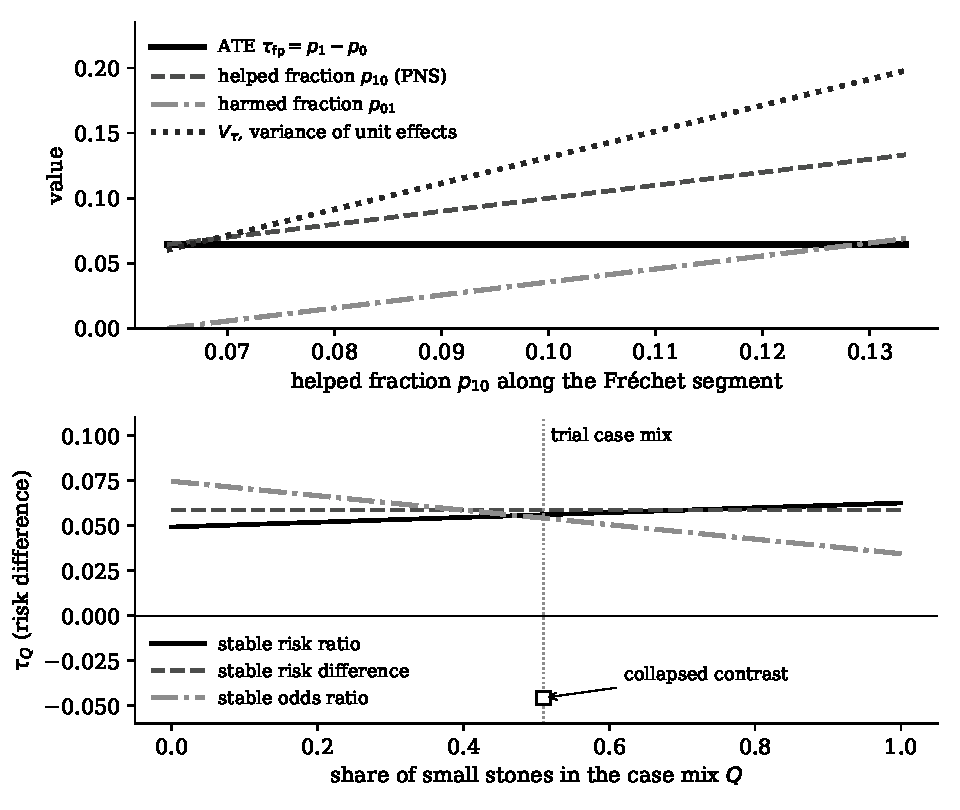
\includegraphics[width=\linewidth]{kidney_ate_urn.pdf}
\caption{Both panels are computed from the kidney stone counts of Table~\ref{fw:tab:simpson}, with no simulation. Top: urns with the small stone margins ($p_1=0.931$, $p_0=0.867$), indexed by the helped fraction $p_{10}$ along the Fr\'echet segment. The ATE is constant (thick solid line); the helped fraction (dashed), the harmed fraction $p_{01}$ (dash dot) and the variance of the unit effects $V_\tau$ (dotted) are not. Bottom: the ATE implied by the effect fitted on each scale against the share of small stones in the urn: risk ratio (solid), risk difference (dashed), odds ratio (dash dot). The dotted vertical line is the observed share, 0.51, and the open square the collapsed contrast, $-0.046$.}
\label{gr:fig:ateurn}
\end{figure}

\section{Transformation models and Haar priors}\label{gr:sec:transform}

Condition C2 of Section~\ref{gr:sec:group} asks the group to act on the observations as well as on the baseline. Let the outcome space be an open interval $I$, let $G$ and the chart $h$ be as in Lemma~\ref{gr:lem:chart}, and take $\mathcal C=I$.

\begin{theorem}\label{gr:thm:recon}
Assume C1 to C3 in the following form: $P_\gamma$ is the law of $h^{-1}(h(\gamma)+\varepsilon)$, where $\varepsilon$ has a fixed known law with density $f$ on $\R$. Then $Y\sim P_\gamma$ implies $gY\sim P_{g\gamma}$, which is C2. Let unit $i$ have control law $P_{\gamma_i}$ and treated law $P_{g\gamma_i}$.
\begin{enumerate}
\item[(a)] Under the comonotone coupling of the potential outcomes, $h(Y_i(1))-h(Y_i(0))=\psi(g)$ for every unit, so the Neyman and Rubin effect on the chart scale equals the group effect $\psi(g)$ for every sample and every configuration of baselines.
\item[(b)] Suppose the baselines $\gamma_i$ are known and $n_1$ treated responses with independent errors are observed. They form a transformation model\index{transformation model} under the action of $G$ on the scale $z_i=h(Y_i)-h(\gamma_i)$. Under the right Haar prior on $g$, the posterior law of the pivot $\psi(g)-\psi(\hat g)$ equals its sampling law given the maximal invariant $a$, for any equivariant estimator $\hat g$. A credible set $\{g:\psi(g)-\psi(\hat g)\in A\}$ of posterior probability $1-\alpha$, with $A$ chosen given $a$ only, therefore has coverage exactly $1-\alpha$, conditionally and unconditionally.
\item[(c)] If $\hat g$ is the maximum likelihood estimate, assumed unique, $f$ is twice differentiable and $j(\hat g)>0$ almost surely, the conditional density of $\hat g$ given $a$ is exactly the Barndorff Nielsen formula $p^{*}(\hat g\mid a;g)=c(a)\,|j(\hat g)|^{1/2}L(g)/L(\hat g)$, with $L$ the likelihood, $j$ the observed information and $c(a)$ a normalizing constant.
\end{enumerate}
\end{theorem}

The proofs of (a) and (c) are in Appendix~\ref{app:groupsproofs} and that of (b) in Appendix~\ref{pg:sec:groups}. The comonotone coupling is rank preservation (Chapter~\ref{ch:gente}), an assumption about the joint law that no experiment can check. Part (b) is Fraser's (1961) structural inference: a Bayesian interval from the right Haar prior is also a confidence interval. With known baselines, $z_i=\psi(g)+\varepsilon_i$ is a location model. An equivariant estimator shifts $\psi(\hat g)$ by the same constant added to every $z_i$. The residuals $a=(z_i-\psi(\hat g))_{i\le n_1}$ form a maximal invariant: samples have the same residuals exactly when they differ by a common shift. The right Haar measure is flat in $\psi(g)$.

So one condition does three jobs, under the assumptions of each part: it makes the Neyman and Rubin effect on the chart scale equal the group effect, the right Haar posterior exactly calibrated and the Barndorff Nielsen formula exact. When it fails, as in the logistic model, $\tau_{\mathrm{fp}}$ depends on the sample (Sections~\ref{gr:sec:group} and~\ref{gr:sec:many}) and, the data being discrete, no nonrandomized interval has exact coverage. For continuous one parameter models with a one dimensional sufficient statistic, exact matching forces a location structure (Lindley 1958), and in general the best available is first order probability matching (Welch and Peers 1963), Jeffreys' prior when $\psi$ is the only parameter.

\begin{remark}\label{gr:rem:nuisance}
With an unknown baseline map $\gamma(\cdot)$ under BART or a horseshoe, the guarantee of exactness in (b) is lost, since the prior on the nuisance is not the right Haar measure of a group containing it. What survives, and only under conditions on the prior for $\gamma$ that remove the bias from shrinkage of the baseline, is a semiparametric Bernstein von Mises approximation for the marginal posterior of $g$ (Castillo 2012; Ray and van der Vaart 2020). The conditions can fail: shrinkage of the baseline leaks into the effect, which is regularization induced confounding\index{regularization induced confounding} (Hahn, Carvalho, Puelz and He 2018; Chapter~\ref{ch:ipw}), and the horseshoe leaks less than the lasso but is not exempt. Ray and van der Vaart repair the bias with a prior adjusted by the propensity score, the idea of the coupled prior\index{coupled prior} of Chapter~\ref{ch:horseshoe}: tell the prior which direction carries the confounding.
\end{remark}

\paragraph{An invariant transport gives a group.} Theorem~\ref{gr:thm:recon} assumes a group, and partial exchangeability does not supply one: it leaves the cell laws $(F_{x,0},F_{x,1})$ unrestricted. For real outcomes, write $F_{x,t}$ also for the distribution function and let $M_x=F_{x,1}^{-1}\circ F_{x,0}$ be the monotone optimal transport map from control to treated in cell $x$ (Nareklishvili, Polson and Sokolov 2026b).

\begin{proposition}\label{gr:prop:transport}
Let $\Pi$ be a partially exchangeable prior under which, almost surely, every cell law has a continuous distribution function that is strictly increasing on all of $\R$. The following are equivalent, $\Pi$ almost surely.
\begin{enumerate}
\item[(i)] There is an increasing bijection $g$ of $\R$ with $F_{x,1}(y)=F_{x,0}(g^{-1}y)$ for all $x$ and $y$, a group action on the observations.
\item[(ii)] The map does not depend on the cell: $M_x=M$ for all $x$.
\end{enumerate}
Then $g=M$, and the smallest group for which (i) holds is the cyclic group generated by $M$. A one dimensional group suffices, since $M$ embeds in a continuous flow $(g^{s})_{s\in\R}$ of increasing homeomorphisms with $g^{1}=M$, but when $M$ is not the identity the flow is not unique.
\end{proposition}

The proof is in Appendix~\ref{app:groupsproofs}, and the embedding is due to Fort (1955). McCullagh's stability axiom therefore has a clean Bayesian form: it restricts the de Finetti measure to arrays whose treatment map is the same in every cell, a restriction of the support of $\Pi$ and not a further exchangeability. For binary and count outcomes the only increasing bijection of the observations is the identity (Lemma~\ref{gr:lem:binary}, whose argument applies to any well ordered set of values), so the group must act on $\mathcal C$, and which chart makes the effect constant is the question of Section~\ref{gr:sec:gap}.

\paragraph{Nonabelian groups and the choice of Haar prior.} Exact calibration requires the right Haar prior\index{Haar measure|textbf} in higher dimensions too (Fraser 1961; Hora and Buehler 1966). Left and right differ only for nonunimodular groups, which excludes abelian and compact groups.

\begin{proposition}\label{gr:prop:affine}
For the affine group\index{affine group|textbf}, with elements $g(y)=\sigma y+\mu$ and $\sigma>0$, the right Haar measure is $d\sigma\,d\mu/\sigma$ and the left Haar measure is $d\sigma\,d\mu/\sigma^{2}$. Treatment 2 after treatment 1 is $g_2g_1(y)=\sigma_2\sigma_1y+(\sigma_2\mu_1+\mu_2)$, whose scale part is order free while the location parts of $g_2g_1$ and $g_1g_2$ differ in general.
\end{proposition}

The proof is in Appendix~\ref{app:groupsproofs}. The additive effect of treatment 2 is therefore defined only relative to an order. When two elements are estimated from independent samples and composed, credible sets for the scale part of the composite stay exact, since its pivot is the product of two independent pivots, but the natural pivot of the location part has a law that depends on the elements, so that calibration does not reach it: the Behrens Fisher phenomenon\index{Behrens Fisher problem}. For normal samples the right Haar prior gives the classical $t$ interval, and the left Haar prior a shorter one that fails already for one sample: its nominal 95 percent interval covers 0.917 at $n=5$ (Exercises~\ref{ex:gr:9} and~\ref{ex:gr:10}).

\paragraph{Lanarkshire.} In the milk experiment of Chapter~\ref{ch:mccullagh}, the gain model is additive, so part (a) makes $\psi$ the group and average effect alike, and the whole difficulty lies in the assignment kernel. Let $U$ be the unrecorded nourishment score, $c<0$ its coefficient in gain, and $x$ the recorded variables. Regression identifies only $\psi^{\dagger}(x)=\psi+c\,\Delta(x)$, where $\Delta(x)<0$ is the milk minus control mean of $U$ at $x$ (teachers favoured the poorly nourished), so $\psi^{\dagger}>\psi$ and the naive comparison overstates the benefit of milk. The likelihood depends on $(\psi,c\Delta)$ only through $\psi^{\dagger}$, so the data can inform how the selection term $c\Delta(x)$ varies with $x$ but not its level. With $c\Delta$ constant in $x$ and a flat prior on $\psi$ independent of it, the posterior of $c\Delta$ is its prior, and a posterior draw of $\psi$ is a posterior draw of $\psi^{\dagger}$ minus an independent prior draw of $c\Delta$. Chapter~\ref{ch:tianpearl}, \emph{Lanarkshire in numbers}, is this analysis. Student's remedy removes the term instead of modelling it: a coin toss inside matched pairs makes the kernel ancillary within pairs, whatever the teachers saw, so the within pair difference has mean $\psi$ and $\psi$ is identified without a prior on the selection term.

\section{Choosing the scale: the information gap}\label{gr:sec:gap}

McCullagh's axiom (Section~\ref{gr:sec:group}) holds on a scale when the effect is the same in every stratum. Data never satisfy it exactly, and the distance from satisfying it is a Kullback and Leibler divergence\index{Kullback Leibler divergence}.

\paragraph{The two theorems.}
Let $X_1,X_2,\dots$ be independent draws, generic observations and not the covariate, from a law $P$ with full support on a finite set, with empirical measure $L_n$.

\begin{theorem}[Sanov 1957]\label{gr:thm:sanov}\index{Sanov theorem@Sanov's theorem|textbf}
For every set $A$ of laws whose closure is the closure of its interior in the simplex,
\[
\lim_{n\to\infty}\frac1n\log\Prob(L_n\in A)=-\inf_{F\in A}\KL(F\,\|\,P).
\]
\end{theorem}

\begin{theorem}[The inverse of Sanov's theorem; Ganesh and O'Connell 1999]\label{gr:thm:isanov}\index{Sanov theorem@Sanov's theorem!inverse of|textbf}
Let the random law $F$ have a Dirichlet prior with positive parameters, and suppose $L_n\to F^{\circ}$. For $A$ as above,
\[
\lim_{n\to\infty}\frac1n\log\Pi(F\in A\mid X_{1:n})=-\inf_{F\in A}\KL(F^{\circ}\,\|\,F).
\]
\end{theorem}

In Sanov's theorem the sampling law $P$ is fixed and the empirical law $F$ varies, giving $\KL(F\,\|\,P)$. In the inverse theorem the limiting empirical law $F^\circ$ is fixed and the candidate population law $F$ varies, giving $\KL(F^\circ\,\|\,F)$. For a Dirichlet prior the reason is visible in the posterior density at $F$, which by Stirling's formula is $\exp\{-n\,\KL(L_n\,\|\,F)+O(\log n)\}$, uniformly on compact subsets of the open simplex. The reverse projection $\arg\min_F\KL(F^{\circ}\,\|\,F)$ is the maximum likelihood projection, where the posterior concentrates under misspecification (Kleijn and van der Vaart 2012; Theorem~\ref{pg:thm:misspec}). Figure~\ref{gr:fig:sanov} compares the two rates for one proportion.

\begin{figure}[ht]
\centering
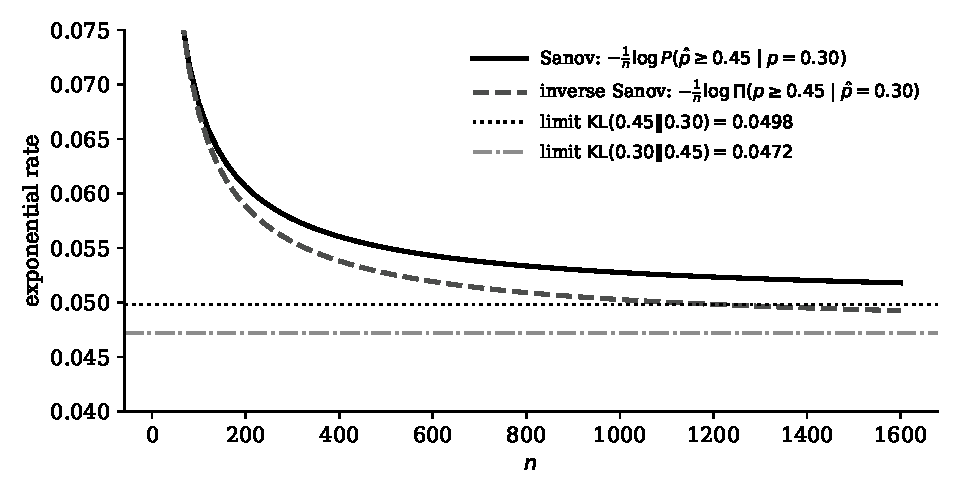
\includegraphics[width=\linewidth]{sanov_vs_inverse.pdf}
\caption{Exact rates for success probability $0.30$ and the set $\{p\ge0.45\}$, $n=20,40,\dots,1600$. Solid line: Sanov, from the binomial tail. Dashed line: the inverse, from the Beta posterior under a flat prior with $\hat p=0.30$. Horizontal lines: the limits $\KL(0.45\,\|\,0.30)=0.0498$ (dotted) and $\KL(0.30\,\|\,0.45)=0.0472$ (dashes and dots).}
\label{gr:fig:sanov}
\end{figure}

\paragraph{Stability classes and information gaps.}
Take strata $x=1,\dots,J$, treatment $t\in\{0,1\}$, design fractions $w_{x,t}>0$, the share of the sample in each cell, and true cell laws $F^{\circ}=(F^{\circ}_{x,t})$. For tables of cell laws write $\KL_w(F\,\|\,F')=\sum_{x,t}w_{x,t}\KL(F_{x,t}\,\|\,F'_{x,t})$ and $\KL_w(F\,\|\,\mathcal S)=\inf_{F'\in\mathcal S}\KL_w(F\,\|\,F')$.

\begin{definition}[Stability class and information gap]\label{gr:def:stable}\index{stability class|textbf}\index{information gap|textbf}
For a group $G$ acting on the baseline parameter space $\mathcal C$, the McCullagh stability class is
\[
\mathcal S_G=\bigl\{F:\ F_{x,0}=P_{\gamma_x},\ F_{x,1}=P_{g\gamma_x}\ \text{for some } \gamma_1,\dots,\gamma_J\in\mathcal C,\ g\in G\bigr\},
\]
where $P_\gamma$ is the outcome law with baseline $\gamma$ and the effect of a member is $\psi(g)$ (for the risk ratio and the risk difference $G$ acts only partially, as Section~\ref{gr:sec:kidney} explains). The information gap of $G$ at $F^{\circ}$ is $D_G=\KL_w(F^{\circ}\,\|\,\mathcal S_G)$.
\end{definition}

The gap is zero exactly when McCullagh's axiom holds on the scale of $G$. At the empirical law $D_G=\mathrm{dev}_G/(2n)$, the deviance of the stable model over twice the sample size, in nats per patient on any scale, so gaps are comparable where effects are not.

\begin{theorem}[The posterior selects the group]\label{gr:thm:select}
Let $\mathcal G$ be a finite collection of groups together with the saturated (heterogeneous) model, each with positive prior probability, a smooth positive prior density on its $d_G$ parameters and a unique interior projection, at which the divergence from $F^{\circ}$ has a nonsingular Hessian in those parameters. Let cell $(x,t)$ receive $nw_{x,t}$ independent draws from $F^{\circ}_{x,t}$. Then almost surely
\[
\frac1n\log\frac{\Pi(\mathcal S_G\mid\text{data})}{\Pi(\mathcal S_H\mid\text{data})}\;\longrightarrow\;D_H-D_G .
\]
More precisely, the log posterior odds equal $n(D_H-D_G)-\tfrac12(d_G-d_H)\log n+O_p(\sqrt n)$, and the fluctuation is $O_p(1)$ when both models contain $F^{\circ}$.
\end{theorem}

\begin{corollary}\label{gr:cor:select}
Suppose also that $d_G<d_{\mathrm{sat}}$ for every group $G$, as for the stable models of this chapter when $J\ge2$, where $d_G=J+1$ and $d_{\mathrm{sat}}=2J$. Under these conditions:
\begin{enumerate}
\item[(i)] if exactly one group $G$ has $D_G=0$, its posterior probability tends to one, the other groups vanish at the exponential rate $D_H$, and the saturated model, which always has $D=0$, at the polynomial rate $n^{-(d_{\mathrm{sat}}-d_G)/2}$;
\item[(ii)] a true stable model beats the saturated model only polynomially, with posterior odds of order $n^{(d_{\mathrm{sat}}-d_G)/2}$, which is $n^{(J-1)/2}$ when the saturated model has an effect in each stratum;
\item[(iii)] if no group is exactly stable, the posterior probability of the saturated model tends to one, and with $D_{\min}=\min_HD_H$ over the groups, attained at $G$, the leading order weights $e^{-nD-\frac12d\log n}$ of the two models cross where $nD_{\min}=\tfrac12(d_{\mathrm{sat}}-d_G)\log n$; this locates the crossing of the weights only, since the fluctuation in the theorem is of larger order.
\end{enumerate}
\end{corollary}

Appendix~\ref{pg:sec:groups} proves the results by a Laplace approximation\index{Laplace approximation} to each marginal likelihood. Inverse Sanov explains the reverse divergence but does not prove these results: $\mathcal S_G$ has empty simplex interior and Dirichlet probability zero. The exponent $D_G$ is prior independent. The stated polynomial factor is for a smooth positive prior; a horseshoe prior on departures from a common effect changes this factor, leaving the exponent alone.

\paragraph{A horseshoe test of stability.} Let the effect in stratum $j$ be $\psi_j=\psi+\eta_j$ for $j=1,\dots,J$, estimated independently by $\hat\psi_j\sim N(\psi_j,\sigma^2J/n)$ with $\sigma$ known and $n/J$ units in each stratum, with a flat prior on $\psi$ and a horseshoe on the departures, $\eta_j\mid\lambda_j,\gscale\sim N(0,\lambda_j^2\gscale^2)$ with $\lambda_j$ half Cauchy. Stability is $\eta_j-\bar\eta=0$ for every $j$, with $\bar\eta$ the average of the $\eta_j$, and it is the boundary point $\gscale=0$ of the alternative. Prior A is a half Cauchy law on $\gscale$ in the units of the data, with density $2/\{\pi(1+\gscale^2)\}$. Prior B puts the global scale in noise units, $\gscale/(\sigma\sqrt{J/n})$, on a half Cauchy law truncated to $[1/J,1]$, the prior for which van der Pas, Szab\'o and van der Vaart (2017a) prove contraction.

\begin{proposition}\label{gr:prop:hstest}
Fix $J\ge2$, let $n\to\infty$ with $n/J$ units in each stratum, and let $\mathrm{BF}_{01}$ be the Bayes factor of stability, $\gscale=0$, against the horseshoe alternative. Write $a_n\asymp_pb_n$ when $a_n/b_n$ and $b_n/a_n$ are both $O_p(1)$.
\begin{enumerate}
\item[(i)] Under stability and prior A, $\mathrm{BF}_{01}\asymp_p\sqrt n/\sigma$ when $J\ge3$, and $\mathrm{BF}_{01}\asymp_p\sqrt n/(\sigma\log n)$ when $J=2$.
\item[(ii)] Under a fixed departure with $\sum_j(\eta_j-\bar\eta)^2>0$ and prior A, $\log\mathrm{BF}_{10}=\{1+o_p(1)\}\,\dfrac{n}{2J\sigma^2}\sum_j(\eta_j-\bar\eta)^2$.
\item[(iii)] Let $\psi$ be known, use prior B, let $J\to\infty$ and let $s=o(J)$ of the $\eta_j$ be nonzero, with $s\ge C\log J$ for a large enough constant $C$. The posterior for $\eta$ contracts in squared error at the near minimax rate $(\sigma^2J/n)\,s\log J$.
\item[(iv)] Under stability and prior B the law of $\mathrm{BF}_{01}$ is the same for every $n$.
\end{enumerate}
\end{proposition}

Appendix~\ref{pg:sec:groups} proves it. Part (i) is the Jeffreys and Lindley asymmetry for a point null\index{Jeffreys Lindley asymmetry}: prior A confirms stability only at rate $\sqrt n$ for $J\ge3$, compared with $n^{(J-1)/2}$ for a smooth positive prior on the $J-1$ contrasts (Corollary~\ref{gr:cor:select}), while part (ii) refutes it exponentially. Stability can therefore be refuted quickly by data and only confirmed slowly. Under prior B it is not confirmed at all: the global scale is tied to the noise, so the alternative shrinks towards the null as $n$ grows, and by part (iv) the Bayes factor has the same law for every $n$. A prior built for estimating the departures, as in part (iii), is a poor one for testing stability.

\paragraph{The kidney stones on three scales.}
Table~\ref{fw:tab:simpson} gives the kidney stone data\index{kidney stone data} and Table~\ref{gr:tab:gaps} the gaps. Figure~\ref{gr:fig:isanov} applies Theorem~\ref{gr:thm:select} with the cell frequencies held at their observed values and $n$ growing. Its curves are leading order weights $e^{-nD_G-\frac12d_G\log n}$ with equal prior model probabilities, $d_G=3$ and $d_{\mathrm{sat}}=4$. They drop the $O(1)$ Laplace terms, the prior density at the projection and the information determinants, so they are not exact posterior probabilities.

At $n=700$ they are $0.38$ on the risk ratio, $0.37$ on the risk difference, $0.23$ on the odds ratio and $0.01$ on heterogeneity, and the split between the risk ratio and the risk difference rests on $0.043$ nats in $nD_G$, less than the terms dropped, so the trial cannot separate these two scales. The odds ratio trails the risk ratio by $0.50$ nats, leading order odds of about $1.6$ to $1$, and the prior density at the projection, one of the dropped terms, moves by about as much when the prior scale of one common effect changes by a factor of $1.6$, so at $n=700$ even that ranking leans on the priors.

The leading order odds of the risk ratio over the odds ratio reach $19$ to $1$ only at about $n=4{,}150$, six times the trial, and heterogeneity overtakes the risk ratio near $n=593{,}000$. The odds ratio, the default of logistic regression and the scale on which McCullagh's group acts most naturally, is the least stable description of these data, by a factor of $64$ in information. 

\begin{table}[ht]
\centering
\caption{Stable estimate, deviance and gap for the kidney stone data ($n=700$, $J=2$, $D_G=\mathrm{dev}_G/1400$). Each stable model has a baseline per stratum and a common effect.}
\label{gr:tab:gaps}
\begin{tabular}{@{}lccc@{}}
\toprule
scale & stable estimate $\hat\psi$ & deviance & $D_G$ (nats per patient) \\
\midrule
log risk ratio & $0.070$ & $0.016$ & $1.1\times10^{-5}$ \\
risk difference & $0.059$ & $0.102$ & $7.3\times10^{-5}$ \\
log odds ratio & $0.357$ & $1.008$ & $7.2\times10^{-4}$ \\
\bottomrule
\end{tabular}
\end{table}

\begin{figure}[ht]
\centering
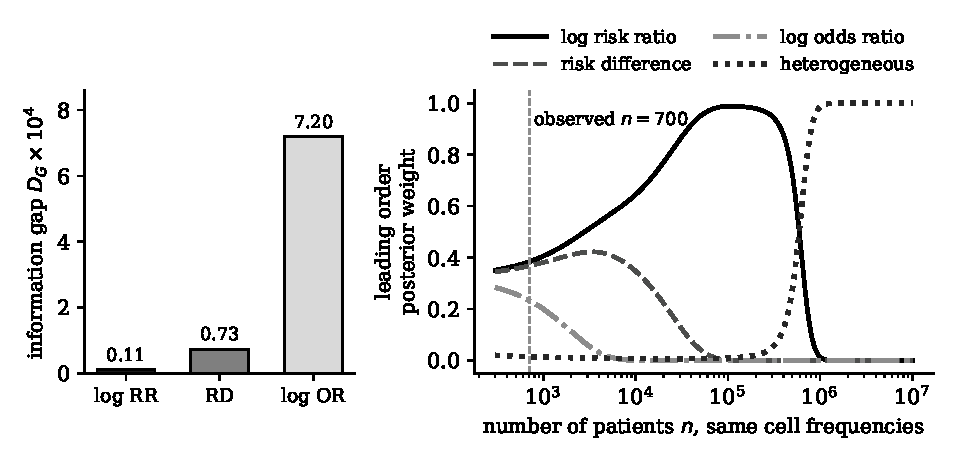
\includegraphics[width=\linewidth]{kidney_inverse_sanov.pdf}
\caption{Kidney stone data. Left: gaps $D_G$ in units of $10^{-4}$ (bars, left to right and darkest to lightest: log risk ratio, risk difference, log odds ratio). Right: leading order weights with equal prior model probabilities and the cell frequencies held fixed, $n$ from 300 to $10^7$. Solid line: log risk ratio. Dashed line: risk difference. Dashes and dots: log odds ratio. Dotted line: heterogeneous model. Vertical dashed line: $n=700$.}
\label{gr:fig:isanov}
\end{figure}

\section{Kidney stones revisited}\label{gr:sec:kidney}

\paragraph{The reversal on three scales.}
On every scale of Figure~\ref{gr:fig:forest} the stratum effects and the stable estimate favour open surgery, while the collapsed contrast favours PCNL with an interval that includes zero\index{Simpson paradox@Simpson's paradox} (Charig and coauthors 1986; Julious and Mullee 1994). The collapsed contrast averages the arms over different case mixes (small stone weights $0.25$ and $0.77$, Section~\ref{gr:sec:margins}), so it changes with the design fractions $w_{x,t}$ and is not covariate equivariant in McCullagh's sense. An exactly stable effect would not depend on the design fractions. Here $D_G>0$ and it does, but it stays between the two stratum effects.

\begin{figure}[ht]
\centering
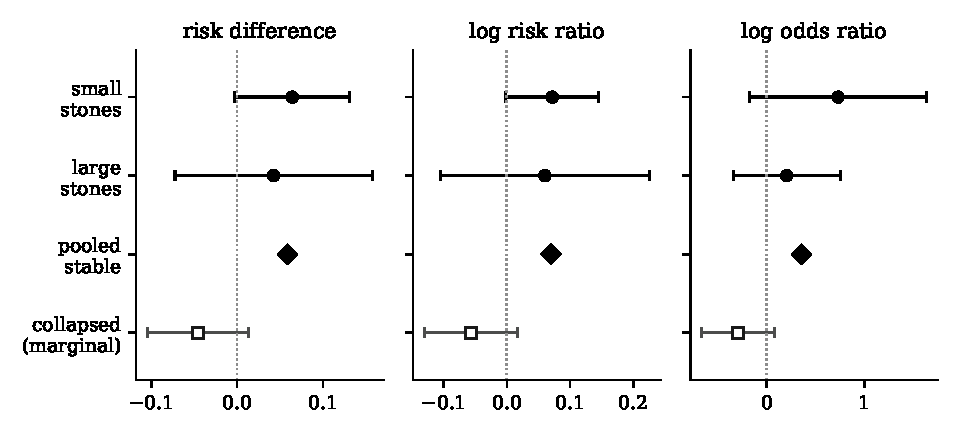
\includegraphics[width=\linewidth]{kidney_forest.pdf}
\caption{Effect of open surgery against PCNL on the risk difference, log risk ratio and log odds ratio scales (panels), from the counts of Table~\ref{fw:tab:simpson}. Filled circles with 95 percent Wald intervals: small and large stones. Filled diamond: stable estimate. Open square with its interval: collapsed contrast. Dotted line: zero.}
\label{gr:fig:forest}
\end{figure}

\paragraph{Closed groups and the risk ratio limit.}
McCullagh would object that neither the risk ratio nor the risk difference is a group action on $\mathcal C=(0,1)$, since $p\mapsto e^{\psi}p$ and $p\mapsto p+\psi$ can leave the interval. Their classes in Table~\ref{gr:tab:gaps} keep the laws whose image stays inside. The logit, the complementary log log and the Aranda Ordaz family (Aranda Ordaz 1981)\index{Aranda Ordaz family|textbf}
\[
h_\lambda(p)=\log\frac{(1-p)^{-\lambda}-1}{\lambda},\qquad\lambda\ge0,
\]
are closed: each $h_\lambda$ maps $(0,1)$ onto $\R$, so translation in its chart is a group action, with $\lambda=1$ the logit and $\lambda\to0$ the complementary log log. The same family applied to the failure probability, $p\mapsto h_\lambda(1-p)$, is a second closed family. A prior on $\lambda$ turns the choice of scale into inference, with its uncertainty reported.

\begin{proposition}\label{gr:prop:limit}
Let $F^{\circ}$ have interior cell probabilities and let $\mathcal S_\lambda$ be the stability class of the chart $p\mapsto h_\lambda(1-p)$, with gap $D_\lambda$, and let $\psi_\lambda$ be the effect of any projection of $F^{\circ}$ on $\mathcal S_\lambda$. As $\lambda\to\infty$, $\lambda^{-1}h_\lambda(1-p)\to-\log p$ uniformly on compact subsets of $(0,1)$. Consequently $D_\lambda\to D_{\mathrm{RR}}$, and when the risk ratio projection is unique, $-\psi_\lambda/\lambda\to\psi_{\mathrm{RR}}$, the stable log risk ratio.
\end{proposition}

The argument is in Appendix~\ref{app:groupsproofs}. For the kidney data (Figure~\ref{gr:fig:closed}) the gap on the failure side decreases at every step of a grid of $\lambda$, from $8.4\times10^{-4}$ at the log log link to the risk ratio value $1.1\times10^{-5}$. On the success side it increases at every step, from $3.6\times10^{-4}$ at the complementary log log to $9.6\times10^{-4}$, where it is flat. The monotonicity is a numerical fact for these data, not part of the proposition. At $\lambda=316$ the stable effect $-\psi_\lambda/\lambda=0.0697$ equals the stable log risk ratio to five decimals.

\begin{figure}[ht]
\centering
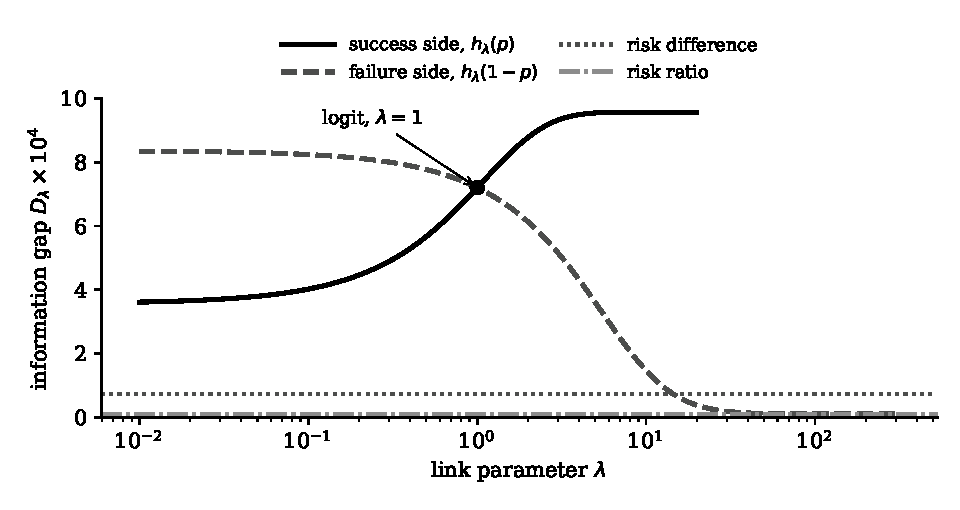
\includegraphics[width=\linewidth]{kidney_closed_groups.pdf}
\caption{Gap $D_\lambda$ in units of $10^{-4}$ against $\lambda$ (log axis) on the grid $10^{k/20}$, kidney stone data. Solid line: $h_\lambda(p)$ on the success probability ($\lambda$ up to 19.95). Dashed line: $h_\lambda(1-p)$ on the failure probability ($\lambda$ up to 316.2). Filled dot: the logit. Horizontal lines: the risk difference gap (dotted) and the risk ratio gap (dashes and dots).}
\label{gr:fig:closed}
\end{figure}

The data prefer a description that McCullagh's axioms exclude, but it is the boundary of a family his axioms admit. On the failure side grid the posterior odds for any two values of $\lambda$ favour the larger at the exponential rate of Theorem~\ref{gr:thm:select}, the difference of their gaps. These pairwise comparisons do not establish that a continuous prior on $\lambda$ sends its mass to the boundary. A Bayesian analysis that respects McCullagh reports the closed group with large $\lambda$: its rescaled effect $-\psi_\lambda/\lambda$ is, to five decimals on these data, the stable log risk ratio, and it remains a valid group action for patients whose baseline risk lies outside the observed range.

\section{Large deviations for causal questions}\label{gr:sec:ld}

This section can be skipped on a first reading. It uses Sanov's theorem and its inverse\index{large deviations|textbf} to put six more questions to the kidney stone data, one to a paragraph. Cells are $(x,t)$ with design fractions $w_{x,t}$, $L_n=(L_{n,x,t})$ holds the empirical cell laws, and $\KL_w$ is as in Section~\ref{gr:sec:gap}.

\paragraph{One gap, two exponents.}
The generalized likelihood ratio statistic for stability on $G$ is $W_n=\KL_w(L_n\,\|\,\mathcal S_G)=\mathrm{dev}_G/(2n)$.

\begin{theorem}[Hoeffding 1965; Bahadur 1967]\label{gr:thm:hoeffding}\index{Hoeffding, Wassily!error exponent of tests|textbf}\index{Bahadur exact slope|textbf}
Let the outcome alphabet have $m$ letters, let there be $C$ cells, let $\mathcal S_G$ be closed and $F^{\circ}$ of full support. (i) For every $F\in\mathcal S_G$, $\Prob_F(W_n\ge\zeta)\le(n+1)^{Cm}e^{-n\zeta}$. (ii) Under $F^{\circ}$, $W_n\to D_G$ almost surely. (iii) If $D_G>0$ and $\{F:\KL_w(F\,\|\,\mathcal S_G)>D_G\}$ meets every neighbourhood of $F^{\circ}$, the $p$ value $p_n=\sup_{F\in\mathcal S_G}\Prob_F(W_n\ge W_n^{\mathrm{obs}})$ satisfies $-n^{-1}\log p_n\to D_G$, so the Bahadur exact slope of the test is $2D_G$.
\end{theorem}

With Theorem~\ref{gr:thm:select} it says (proof in Appendix~\ref{app:groupsproofs}) that the $p$ value for stability and the posterior odds for stability against the saturated model decay at the same exponential rate $D_G$. Both exponents carry fluctuations of order $\sqrt n$, and the polynomial factors differ: the type count $(n+1)^{Cm}$, only an upper bound, against the Lindley factor $n^{(d_{\mathrm{sat}}-d_G)/2}$ of a smooth positive prior.

\paragraph{Confounding as a Sanov event.}
Randomization with a common treatment probability makes $T$ independent of $X$, so the table of $(X,T)$ is drawn from $P_X\otimes P_T$, and by Sanov's theorem the probability of an empirical table at least as dependent as the observed one is $\exp\{-n\hat I_{\mathrm{obs}}+O(\log n)\}$, because $\KL(F\,\|\,P_X\otimes P_T)=I_F(X;T)+\KL(F_X\,\|\,P_X)+\KL(F_T\,\|\,P_T)$ and with $P_X$ and $P_T$ set at the observed margins the infimum is $\hat I_{\mathrm{obs}}$, attained by the observed table itself. In the kidney data the mutual information\index{mutual information|textbf} is $\hat I(X;T)=0.144$ nats, so $n\hat I=100.7$ and the probability is of order $10^{-44}$, which shows only that the allocation was not randomized with a common probability: large stones went to open surgery. We do not decompose the reversal into informations, since mutual information carries no sign and, under randomization, $I(T;Y)-I(T;Y\mid X)=-I(X;T\mid Y)$ need not vanish.

\paragraph{The conditional limit theorem and ancillarity.}
McCullagh holds (Section~\ref{gr:sec:group}) that randomization makes the assignment ancillary\index{ancillarity!large deviation content}, and the conditional limit theorem of Csisz\'ar (1984)\index{conditional limit theorem|textbf} gives a sharp form of this: conditional on $L_n$ falling in a closed convex set $A$ of laws with nonempty interior, an event of positive probability, the law of a single observation converges to the I projection\index{I projection|textbf} $F^{\dagger}=\arg\min_{F\in A}\KL(F\,\|\,P)$.

\begin{proposition}\label{gr:prop:ancillary}
Let $P$ be a law of $(X,T,Y)$ and let $A$, as above, constrain only the $(X,T)$ margin, for example $A=\{F:F(T=1\mid X=x)\ge\delta\}$, an observed imbalance. Then $F^{\dagger}_{Y\mid X,T}=P_{Y\mid X,T}$. Consequently conditioning on the imbalance leaves every cell law unchanged, and with it every functional of the cell laws alone, including the stable effect $\psi$ of a group on which the data are exactly stable, but in general changes the collapsed contrast.
\end{proposition}

Appendix~\ref{app:groupsproofs} proves it. A rare imbalance tilts $P_X\otimes P_T$ exponentially while leaving the outcome mechanism untouched.

\paragraph{Pythagoras and the logit group.}
\begin{theorem}\label{gr:thm:pyth}\index{Pythagorean identity|textbf}
For binary outcomes the logit stability class $\mathcal S_{\mathrm{logit}}$ is an exponential family with canonical parameters $(\gamma_1,\dots,\gamma_J,\psi)$ and sufficient statistics the stratum success counts and the treated success total. If $F^*$ is its maximum likelihood point for the empirical law $\hat F=L_n$, then for every $F\in\mathcal S_{\mathrm{logit}}$,
\[
\KL_w(\hat F\,\|\,F)=\KL_w(\hat F\,\|\,F^*)+\KL_w(F^*\,\|\,F).
\]
\end{theorem}

The identity (proof in Appendix~\ref{app:groupsproofs}) belongs to the maximum likelihood projection and fails in general for the log risk ratio class, whose chart curves the family: Figure~\ref{gr:fig:pyth} shows residuals below $10^{-9}$ along the logit family and down to $-3.1\times10^{-4}$ along the log risk ratio family. The risk difference class is a mixture family, and for it the dual identity holds with the divergence the other way round: if every stratum and arm of the data shows both outcomes and $F^\dagger$ is the I projection of $\hat F$ on the class, then
\[
\KL_w(F\,\|\,\hat F)=\KL_w(F\,\|\,F^\dagger)+\KL_w(F^\dagger\,\|\,\hat F)
\]
for every $F$ in the class (Csisz\'ar 1975).

On the logit group $D_{\mathrm{logit}}=7.2\times10^{-4}$ is the information in the three factor interaction of the $X\times T\times Y$ table. The logit has the cleaner geometry; the risk ratio has the smaller gap.

\begin{figure}[ht]
\centering
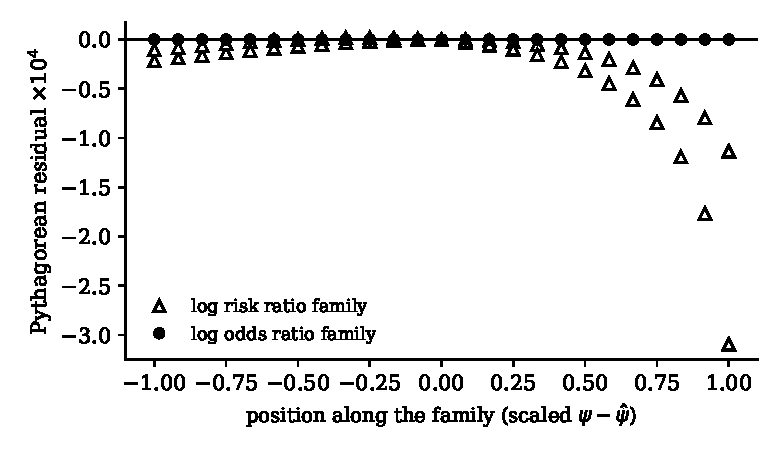
\includegraphics[width=0.9\linewidth]{kidney_information_pythagoras.pdf}
\caption{Pythagorean residual $\KL_w(\hat F\,\|\,F)-\KL_w(\hat F\,\|\,F^*)-\KL_w(F^*\,\|\,F)$ times $10^4$, kidney stone data, for comparison laws $F$ along the logit family (filled circles) and the log risk ratio family (open triangles). The effect of $F$ takes 25 equally spaced values within $0.6$ (logit) or $0.06$ (log risk ratio) of the estimate, with the fitted baselines or with the two stratum baselines shifted by $0.15$ and $-0.1$ ($0.01$ and $-0.01$) on the chart. Horizontal axis: the effect of $F$ minus the estimate, scaled by its largest value.}
\label{gr:fig:pyth}
\end{figure}

\paragraph{Posterior large deviations for the effect.}
The Laplace argument behind Theorem~\ref{gr:thm:select} also gives the posterior of the effect itself. Define the profile rate function of the stable effect on $G$ at the empirical law,
\[
J_G(\psi)=\inf\bigl\{\KL_w(L_n\,\|\,F):\ F\in\mathcal S_G,\ \psi(F)=\psi\bigr\}-W_n,
\]
so that $nJ_G(\psi)$ is half the profile deviance and $J_G$ vanishes at the maximum likelihood estimate $\hat\psi$. Profiling maximizes over baselines; the posterior integrates over baselines and the effect. Thus $e^{-nJ_G(\psi_0)}$ supplies only a tail's exponential rate, while the signed root $r(\psi)$ adds the leading factor.

\begin{proposition}\label{gr:prop:effect}
Under the conditions of Theorem~\ref{gr:thm:select} and a smooth positive prior on $\mathcal S_G$, suppose that at every fixed $\psi$ in the range considered the conditional maximum of the likelihood over the baselines is unique and interior, varies smoothly with $\psi$, and has baseline information that stays positive definite on compact sets, and that $J_G$ is smooth, vanishes only at $\hat\psi$, increases away from it with $J_G'(\psi)\neq0$ for $\psi\neq\hat\psi$, and has $J_G''(\hat\psi)>0$. Then for intervals $A$,
\[
\Pi(\psi\in A\mid\text{data})=\exp\Bigl\{-n\inf_{\psi\in A}J_G(\psi)+O_p(\log n)\Bigr\}.
\]
The signed root $r(\psi)=\operatorname{sign}(\psi-\hat\psi)\sqrt{2nJ_G(\psi)}$ satisfies $\Pi(\psi\le\psi_0\mid\text{data})=\Phi(r(\psi_0))\{1+O(n^{-1/2})\}$ when $\psi_0-\hat\psi=O(n^{-1/2})$. For fixed $\psi_0$ its relative error is $O(1)$.
\end{proposition}

The proof is in Appendix~\ref{pg:sec:groups}. Table~\ref{gr:tab:profile} gives, for the kidney data, the probability that open surgery is no better.

\begin{table}[ht]
\centering\small\setlength{\tabcolsep}{4pt}
\caption{Posterior probability that the stable effect is at most zero, kidney stone data, $n=700$. The prior is flat on the baselines and the effect in the coordinates of each chart, restricted to valid probabilities. The last column is a numerical quadrature.}
\label{gr:tab:profile}
\begin{tabular}{@{}lccccc@{}}
\toprule
scale & $\hat\psi$ & $10^3J_G(0)$ & $e^{-nJ_G(0)}$ & $\Phi(-\sqrt{2nJ_G(0)})$ & exact $\Pi(\psi\le0)$ \\
\midrule
risk difference & $0.059$ & $2.39$ & $0.19$ & $0.034$ & $0.040$ \\
log risk ratio & $0.070$ & $2.45$ & $0.18$ & $0.032$ & $0.041$ \\
log odds ratio & $0.357$ & $1.74$ & $0.29$ & $0.059$ & $0.059$ \\
\bottomrule
\end{tabular}
\end{table}

Figure~\ref{gr:fig:effectld} shows the profile rate and the posterior density behind the table. The exponent alone is within a factor of five, and the signed root is within $0.001$ of the exact posterior on the odds ratio scale and within $0.01$ on the other two. The collapsed analysis, with independent uniform priors on the four cell probabilities ($400{,}000$ posterior draws), puts $0.057$ on PCNL being no better and $0.943$ on its being no worse. It is as confident as the stable analyses, in the opposite direction, because the collapsed contrast averages the two arms over different case mixes (Chapter~\ref{ch:frameworks} explains why the stratified numbers govern).

\begin{figure}[ht]
\centering
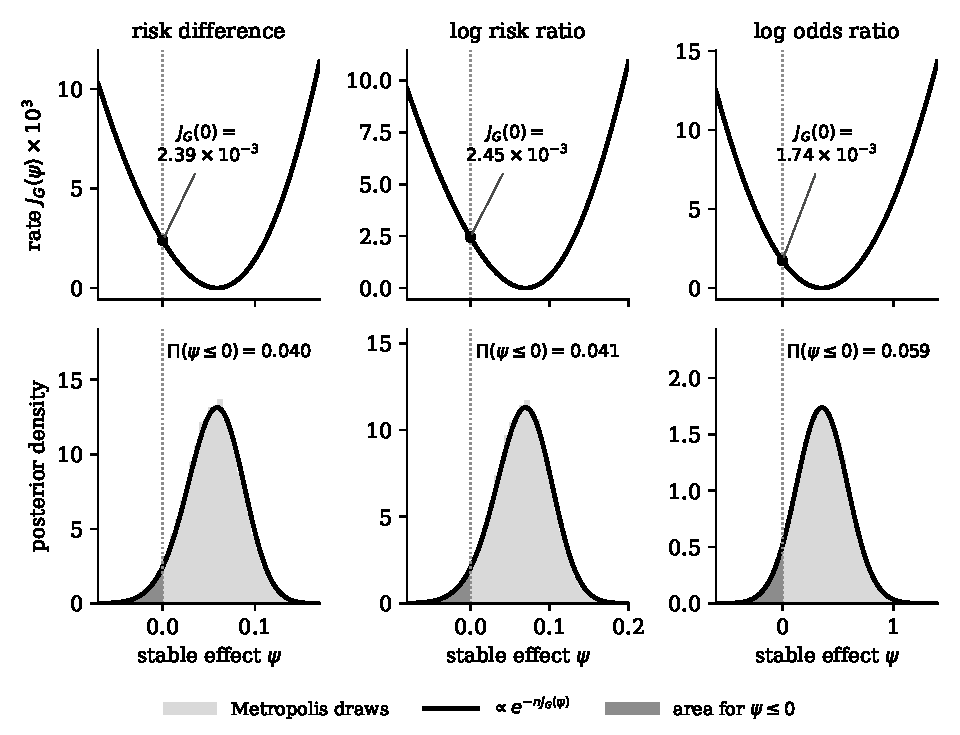
\includegraphics[width=\linewidth]{kidney_effect_ld.pdf}
\caption{Kidney stone data, $n=700$; columns are the risk difference, log risk ratio and log odds ratio. Top: $J_G(\psi)$ times $10^3$, with $J_G(0)$ marked. Bottom: posterior density of the stable effect. Light gray histogram: a Metropolis chain with flat priors on the chart coordinates (seed 7, 260,000 steps, 20,000 discarded, every fifth kept draw shown, baseline proposal standard deviations $0.02$, $0.03$ and $0.25$ in the three columns, and effect proposal standard deviations $0.016$, $0.024$ and $0.20$). Black line: $e^{-nJ_G(\psi)}$, normalized. Dark gray area: $\psi\le0$, labelled with the exact $\Pi(\psi\le0)$ from quadrature. Dotted vertical lines: zero.}
\label{gr:fig:effectld}
\end{figure}

\paragraph{Transport and the Donsker Varadhan formula.}
McCullagh's covariate equivariance is a transport property: the effect should mean the same thing in a population with a different case mix $Q'$. The Donsker and Varadhan formula\index{Donsker Varadhan formula|textbf} (Donsker and Varadhan 1975), the variational form of Sanov's theorem, prices the move. Section~\ref{fw:sec:transport} reweights stratum effects over the target's case mix\index{transportability}; the question here is how far the answer shifts.

\begin{proposition}\label{gr:prop:dv}
Let $\psi_G(x)$ be the stratum effect on the scale of $G$, with range $R_G=\max_x\psi_G(x)-\min_x\psi_G(x)$, and $\bar\psi_G(Q)=\sum_xQ_x\psi_G(x)$ its average over the case mix $Q$. Then
\[
|\bar\psi_G(Q')-\bar\psi_G(Q)|\;\le\;R_G\,\|Q-Q'\|_{\mathrm{TV}}\;\le\;R_G\sqrt{\tfrac12\KL(Q'\,\|\,Q)}.
\]
If the data are exactly stable on $G$, $R_G=0$ and transport is free on that scale. When the baselines differ across strata and the effect is not zero, other scales generally lack this property.
\end{proposition}

Appendix~\ref{app:groupsproofs} gives the proof. Transporting the kidney trial, with case mix $Q=(0.51,0.49)$ for small and large stones, to a population of small stones only, with $\KL(Q'\,\|\,Q)=0.67$, moves the average stratum effect by $0.011$ on the risk difference scale (bound $0.013$), $0.0057$ on the log risk ratio scale (bound $0.0067$) and $0.26$ on the log odds ratio scale (bound $0.30$): $18$, $8$ and $72$ percent of the stable estimate. On these data the scale with the smallest information gap transports most cheaply in the sense of Donsker and Varadhan.

\section{In practice}\label{gr:sec:practice}

\paragraph{The target.} The target of this chapter is a stable effect and the averages it supports, all from one posterior. The posterior of $\psi$ on each candidate scale comes from the stable model on that scale, and an average $\tau_Q$ comes from the same draws by the accounting identity of Chapter~\ref{ch:mccullagh}, once for each case mix $Q$ of interest. The finite population effect $\tau_{\mathrm{fp}}$ also needs a joint prior for the pair of potential outcomes, because the likelihood involves only the margins, and the fraction helped is a target only as an interval. For the kidney stones the target is $\psi$ for open surgery against the percutaneous procedure on each of three scales: the posterior probability that open surgery is no better lies between 0.040 and 0.059, and the standardized average effect on the risk difference scale, computed at the observed stratum rates, is 0.054.

\paragraph{What the analyst does differently.} The analyst reports the effect and the averages as different things. She fits the stable model on each candidate scale, or puts a prior on the Aranda Ordaz parameter, and reports the information gap of each, so that the reader sees how far the data are from McCullagh's axiom on the scale used. Each average $\tau_Q$ is a separate number tied to a case mix and a decision. She does not call the fraction helped or the variance of the unit effects identified by a randomized trial, and gives the Fr\'echet interval or the joint prior that fills it. Where she controls the design she allocates both arms in proportion to the strata, and where she does not she reports the standardized contrast. A claim of exact calibration names its conditions, a transformation model with known baselines and the right Haar prior, and with a baseline under BART or a horseshoe the interval is reported as approximate. Stability is a commitment that data refute quickly and confirm slowly, at a rate set by the prior on the departures (Corollary~\ref{gr:cor:select} and Proposition~\ref{gr:prop:hstest}), so she names that prior.

\paragraph{Against DML.} Where the target is one average, such as the marginal risk difference of a randomized trial, DML is adequate, as Chapter~\ref{ch:mccullagh} says, and cheaper than posterior computation. An average does not say on which scale the effect is stable: the risk difference, the risk ratio and the odds ratio of the kidney stones each need their own orthogonal score, and none of the three reports that the gaps differ by a factor of 64. Nor does an average say how it moves with the case mix, which on these data it does in opposite directions on the risk ratio and odds ratio scales. And no estimator, orthogonal or not, narrows the fraction helped below its Fr\'echet interval or pins down the term $S_\tau^2/n$ (Proposition~\ref{gr:prop:fpc}), because both depend on the coupling of the pairs, which the margins leave free. The posterior carries the stable effect, the averages and the interval from one fit. The limits are the group and the baseline. The group is a modelling commitment: the information gap ranks the scales in hand and cannot propose a better one. With a flexible baseline under BART or a horseshoe the exact calibration of Theorem~\ref{gr:thm:recon} is guaranteed only approximately, and only under conditions on the prior for the baseline, with the leakage from shrinkage that Chapter~\ref{ch:horseshoe} meets with the coupled prior.

\section*{Notes}

McCullagh (2002, 2022) gives the process view, the group effect and the requirement that it be stable. Battey and Edgar (2026) state that the group effect and the potential outcomes effect agree for every sample exactly under the conditions C1 to C3 of Section~\ref{gr:sec:group}, and note that C1 and C2 make the model a transformation family. Part (a) of Theorem~\ref{gr:thm:recon} restates their agreement on the chart scale with the coupling made explicit; what is ours is the observation that the same conditions also give the exact calibration of parts (b) and (c). For part (b) the location case is due to Fisher (1934) and Pitman (1939) and the group version to Fraser (1961), and Hora and Buehler (1966) give the confidence property. Part (c) is Barndorff Nielsen's (1983) result that his formula is exact for every transformation model.

Neyman (1923) gives the variance of the difference in means under complete randomization. The kidney stone counts are Charig, Webb, Payne and Wickham (1986). The information theory of Sections~\ref{gr:sec:gap} and~\ref{gr:sec:ld}, divergence, the method of types and large deviations, is the background treated in the authors' book, Polson and Sokolov (2026c), \emph{Elements of Bayes and Information Theory}. 

\begin{exercises}
\item\label{ex:gr:1} Let $g_\psi(p)=e^{\psi}p/\{1+(e^{\psi}-1)p\}$ be the action of the logit group on a risk $p$. (a) Show that $g_{\psi_1}\circ g_{\psi_2}=g_{\psi_1+\psi_2}$, so that $\psi\mapsto g_\psi$ is an isomorphism of $(\R,+)$ with a group of maps of $(0,1)$. (b) Let $\psi>0$. Show that the risk difference $g_\psi(p)-p$, as a function of the baseline log odds $\gamma=\logit p$, is largest at $\gamma=-\psi/2$, where it equals $\tanh(\psi/4)$. (c) Deduce that $\tau_Q(\psi)\le\tanh(\psi/4)$ for every $Q$ and every $\psi>0$, and, using $e^{2\operatorname{artanh}\tau}=(1+\tau)/(1-\tau)$, that an average effect of $0.2$ needs an odds ratio of at least $\{(1+0.2)/(1-0.2)\}^2=2.25$.
\item\label{ex:gr:2} Let $I_i$ indicate that unit $i$ is assigned to treatment under complete randomization with $n_1$ of $n$ units treated. Using $\Prob(I_i=1)=n_1/n$ and $\mathrm{Cov}(I_i,I_j)=-n_1(n-n_1)/\{n^2(n-1)\}$ for $i\ne j$, derive the variance of $\bar Y_1$ in Proposition~\ref{gr:prop:fpc} for a binary urn $\{Y_i(1)\}$ with a proportion $p_1$ of ones. Evaluate it for $n=10$, $n_1=5$ and four ones, and check the value $0.0267$ against the hypergeometric distribution of the number of ones among the five units drawn.
\item\label{ex:gr:3} Take $n=20$ units, five of each of the four types $(Y(1),Y(0))=(1,1),(1,0),(0,1),(0,0)$, so that $\tau_{\mathrm{fp}}=0$ although half the units are affected. Draw 100,000 complete randomizations with $n_1=n_0=10$, compute the difference in means $\hat\tau$ for each, and report its empirical variance. Compare it with the variance of Proposition~\ref{gr:prop:fpc}, computed from the urn with divisor $n-1$, and with the conservative value that drops the term $S_\tau^2/n$. Which of the two does the simulation match, and by what factor does the other overstate it?
\item\label{ex:gr:4} A randomized trial has $p_1=0.8$ and $p_0=0.5$. (a) Give the bounds of Proposition~\ref{gr:prop:frechet} on the fraction helped $p_{10}$, and the four type fractions at each end of the interval. (b) Give the bounds of Proposition~\ref{gr:prop:sharpvar} on $V_\tau$, and check both directly from the type fractions at the two ends. (c) Since $S_\tau^2/n=V_\tau/(n-1)$, find the range of the amount by which Neyman's conservative variance overstates $\mathrm{Var}(\hat\tau)$ when $n=100$.
\item\label{ex:gr:5} Let the outcomes be binary. (a) Show that $f:\{0,1\}^2\to\R$ is separable if and only if $f(1,1)+f(0,0)=f(1,0)+f(0,1)$. (b) Show that $f(a,b)=(a-b)^2$ and $f(a,b)=\one\{a=1,b=0\}$ are not separable, by giving two joint laws with margins $p_1=p_0=\tfrac12$ for which $\int f\,dF$ differs. (c) For margins with $0<p_0,p_1<1$ and a function $\kappa$ on $\{-1,0,1\}$, show that the mean of $\kappa(a-b)$ is the same for every joint law with those margins only if $\kappa(1)+\kappa(-1)=2\kappa(0)$, and that the mean is then an affine function of the ATE.
\item\label{ex:gr:6} A stratified experiment has two strata of 200 units each. In the first stratum 50 units are treated and 150 are controls, and in the second 150 are treated and 50 are controls. The stratum means of $Y(1)$ and $Y(0)$ are $0.95$ and $0.90$ in the first stratum and $0.55$ and $0.50$ in the second. (a) Compute $\tau_{\mathrm{fp}}$ and the expected value of the collapsed contrast of Proposition~\ref{gr:prop:strat}. (b) Derive the bias of the collapsed contrast for general allocations $n_{x,t}$, and show that it vanishes for every urn exactly when both arms are allocated in proportion to the stratum sizes.
\item\label{ex:gr:7} For a Bernoulli law with success probability $0.30$ and the set $\{p\ge0.45\}$, compute (a) $\KL(0.45\,\|\,0.30)$ and $\KL(0.30\,\|\,0.45)$; (b) for $n=100$, $400$ and $1600$, the Sanov rate $-n^{-1}\log\Prob\{\mathrm{Bin}(n,0.30)\ge0.45n\}$ and the rate $-n^{-1}\log\Pi(p\ge0.45\mid\text{data})$ when the sample proportion is $0.30$ and the prior is flat, so that the posterior is Beta$(0.3n+1,\,0.7n+1)$. Compare each rate with its limit, as in Figure~\ref{gr:fig:sanov}, and say which of Theorems~\ref{gr:thm:sanov} and~\ref{gr:thm:isanov} each limit belongs to.
\item\label{ex:gr:8} Take the gaps of Table~\ref{gr:tab:gaps}, $d_G=3$ for each of the three groups, $d_{\mathrm{sat}}=4$ for the heterogeneous model with gap zero, equal prior probabilities on the four models and the leading order weights $e^{-nD_G-\frac12d_G\log n}$ of Section~\ref{gr:sec:gap}. (a) Normalize the weights to sum to one at $n=700$ and compare them with the values quoted in the text. (b) Find the $n$ at which the leading order odds of the risk ratio over the odds ratio reach $19$ to $1$, and say why the polynomial factors play no part in the answer.
\item\label{ex:gr:9} (a) For the affine group with composition $(\sigma_2,\mu_2)(\sigma_1,\mu_1)=(\sigma_2\sigma_1,\sigma_2\mu_1+\mu_2)$, compute the Jacobians of the maps $g\mapsto gg_0$ and $g\mapsto g_0g$ on $(\sigma,\mu)$, and show that $d\sigma\,d\mu/\sigma$ is invariant under the first and $d\sigma\,d\mu/\sigma^2$ under the second. (b) For $n$ independent $N(\mu,\sigma^2)$ observations with mean $\bar y$ and variance $s^2$ (divisor $n-1$), show that the prior $\sigma^{-k}\,d\sigma\,d\mu$ gives $\mu$ a Student $t$ posterior with $n+k-2$ degrees of freedom and scale $s\{(n-1)/(n(n+k-2))\}^{1/2}$, and write out the right Haar case, $k=1$, and the left Haar case, $k=2$.
\item\label{ex:gr:10} Draw $n$ independent $N(0,1)$ observations, for $n=3$ and $n=5$, with 100,000 replications for each $n$. For each sample form the 95 percent credible interval for $\mu$ under the right Haar prior, $\bar y\pm t_{n-1}\,s/\sqrt n$, and under the left Haar prior, $\bar y\pm t_n\,s\sqrt{n-1}/n$, where $t_\nu$ is the $0.975$ quantile of the Student $t$ distribution with $\nu$ degrees of freedom. Report the fraction of replications in which each interval contains $\mu=0$, and compare the left Haar fraction with the exact coverage $\Prob(|T_{n-1}|\le t_n\sqrt{(n-1)/n})$, where $T_{n-1}$ has a Student $t$ distribution with $n-1$ degrees of freedom.
\end{exercises}

\part{Double Machine Learning}
\chapter{What Double Machine Learning Assumes}\label{ch:dml}

\begin{tcolorbox}[colback=gray!6,colframe=gray!50,title=In brief,fonttitle=\normalfont\itshape,coltitle=black,colbacktitle=gray!15,boxrule=0.4pt,arc=1pt]
Double machine learning estimates one effect while flexible learners fit the nuisance functions around it. A Neyman orthogonal score makes nuisance errors enter as products, and cross fitting removes overfitting bias. The main theorem gives root $n$ normal inference when the treatment keeps some variation after adjustment and the treatment error times the sum of the treatment and outcome errors is $o_p(n^{-1/2})$, a condition that includes the square of the treatment error. The partially linear score estimates a variance weighted average of effects, and its estimated denominator is not an overlap diagnostic.
\end{tcolorbox}

\section{The question DML answers}\label{sec:dml:question}

A household survey records, for 9,915 households, whether the employer offers a 401(k) plan, the household's net financial assets\index{net financial assets|textbf}, and nine other characteristics: age, income, years of education, family size, and indicators for marriage, two earner households, a defined benefit pension, an individual retirement account and home ownership. Eligible households hold 19.6 thousand dollars more in financial assets than the others. Much of that gap is income. Richer households tend to work for employers who offer plans, and richer households hold more assets whatever a plan does. The analyst wants what is left of the gap once income and the other characteristics are held fixed, and she does not know the form in which they matter.

Least squares with the nine characteristics entering linearly is the first thing to try. Chapter~\ref{ch:k401} shows that it leaves confounding behind: the estimate is 5.9 thousand dollars, against 9.8 when the nine characteristics are expanded into 54 terms. A flexible learner such as a lasso or a random forest can find the right form, but it converges slowly, and its error passes into the estimate of the effect.

Double machine learning\index{double machine learning|textbf} (DML)\index{DML|see{double machine learning}} estimates a low dimensional causal parameter at the $\sqrt{n}$ rate while high dimensional nuisance functions are estimated by slowly converging flexible learners. Chernozhukov and coauthors (2018) do it by combining an estimating equation\index{estimating equation|textbf} insensitive to small nuisance errors with sample splitting to remove overfitting bias\index{overfitting bias|textbf}. The nuisance functions need no model. The learner is a black box, and all the theory asks of it is a rate of convergence in $L_2$.

We try to be fair to the method. The criticism belongs to Chapter~\ref{ch:critique}.

\section{The partially linear model and partialling out}\label{sec:dml:plm}

If the covariates predicted eligibility exactly, households with the same characteristics would all have the same status, and nothing would be left to compare. The effect can only be learned from the part of treatment that the covariates do not explain. Robinson's (1988) partially linear model\index{partially linear model|textbf} puts this part at the center,
\begin{align}
Y &= \tau T + g(X) + \varepsilon, & \E(\varepsilon \mid X, T) &= 0, \label{eq:plm1}\\
T &= m(X) + \nu, & \E(\nu \mid X) &= 0. \label{eq:plm2}
\end{align}
The target is $\tau$, with true value $\tau_0$; the nuisance functions\index{nuisance function|textbf}\index{nuisance parameter|see{nuisance function}} are $g$ and $m$, with $m(x) = e(x)$ for a binary treatment\index{propensity score}. The condition $\E(\varepsilon \mid X, T) = 0$ makes the unexplained treatment $\nu$ exogenous, identifying $\tau_0$ from how $Y$ moves with $\nu$.

The naive approach estimates $g$ by a machine learner, say a lasso or a random forest, then regresses $Y - \hat g(X)$ on $T$. This fails: regularization biases\index{regularization bias|textbf} $\hat g$, and since $T$ is correlated with $X$ the bias leaks into the estimate of $\tau$. The leak is of the order of the error in $\hat g$, slower than $n^{-1/2}$ for high dimensional learners, so the naive estimator is not $\sqrt{n}$ consistent.

Robinson's insight was to partial out\index{partialling out|textbf}\index{Robinson, Peter M.!partialling out|textbf} $X$ from both $Y$ and $T$. Define $\ell(X) = \E(Y \mid X) = \tau m(X) + g(X)$. Then
\[
Y - \ell(X) = \tau \{T - m(X)\} + \varepsilon,
\]
and $\tau$ is the coefficient in a regression of one residual on the other. With fitted $\hat\ell$ and $\hat m$ in place of the truth the residuals are $\hat V_{Y,i} = Y_i - \hat\ell(X_i)$ and $\hat V_{T,i} = T_i - \hat m(X_i)$, and the estimator has a closed form,
\begin{equation}
\hat\tau = \frac{\sum_{i=1}^n \hat V_{T,i}\,\hat V_{Y,i}}{\sum_{i=1}^n \hat V_{T,i}^2}.
\label{eq:dml:ratio}
\end{equation}
Errors in $\hat\ell$ and $\hat m$ now cost the estimate only at second order, a statement that Section~\ref{sec:dml:exact} makes exact.

 A household whose eligibility the covariates predict well has a small $\hat V_{T,i}$ and adds little; the estimate is built from the households that the covariates leave undecided. The denominator measures how many such households there are. Its population version is $J_0 = \E\nu^2 = \E\,\mathrm{Var}(T \mid X)$, which for a binary treatment equals $\E[e(X)\{1 - e(X)\}]$ and shrinks as propensities approach zero or one. This is the content of overlap\index{overlap}: a household whose treatment status is nearly determined by its covariates has no comparable household with the other status. When $J_0$ is small the estimator divides by a number near zero, and a small error in the numerator becomes a large error in $\hat\tau$. Section~\ref{sec:dml:thm} states the overlap requirement, and Chapter~\ref{ch:critique} shows what happens as it fails (Proposition~\ref{crit:prop:dufour}).

\section{Scores and Neyman orthogonality}\label{sec:dml:score}

Suppose the outcome error $\delta_g = \hat g - g$ lines up with the part of treatment the covariates explain. The plug in estimator, which regresses $Y - \hat g(X)$ on $T$, attributes the misfit to treatment: to first order it moves by $-\E\{m(X)\,\delta_g(X)\}/\E(T^2)$, which shrinks no faster than the learner's own error. A score is Neyman orthogonal\index{Neyman orthogonality!and bias|textbf} when no such first order term exists (Neyman\index{Neyman, Jerzy!orthogonal scores|textbf} 1959).

\begin{definition}[Neyman orthogonal score]
Let $\psi(W; \tau, \eta)$ be a score function of the data $W$, the target $\tau$ and a nuisance parameter $\eta$, with $\E\psi(W; \tau_0, \eta_0) = 0$ at the truth. The score is Neyman orthogonal\index{Neyman orthogonality|textbf}\index{orthogonal score|see{Neyman orthogonality}}\index{orthogonal moment|see{Neyman orthogonality}} if the G\^ateaux derivative\index{Gateaux derivative|textbf} with respect to $\eta$ vanishes at the truth:
\[
\left.\frac{\partial}{\partial r} \E\, \psi\bigl(W; \tau_0, \eta_0 + r(\eta - \eta_0)\bigr)\right|_{r=0} = 0
\]
for all $\eta$ in a suitable neighbourhood.
\end{definition}

For the partially linear model the Robinson score, with nuisance parameter $\eta = (\ell, m)$, is
\begin{equation}
\psi(W; \tau, \ell, m) = \{Y - \ell(X) - \tau(T - m(X))\}\{T - m(X)\}.
\label{eq:robscore}
\end{equation}
We write $\delta_m = \hat m - m$ and $\delta_\ell = \hat\ell - \ell$ for the errors of the fitted nuisance functions\index{nuisance function}, and $\|f\| = \{\E f(X)^2\}^{1/2}$ and $\langle f, h\rangle = \E f(X)h(X)$ for a function of the covariates held fixed while $X$ is a fresh draw.

\begin{proposition}\label{dml:prop:orth}
Let $\delta_\ell$ and $\delta_m$ be square integrable functions of $X$, and let $\varepsilon$ and $\nu$ have finite second moments. Under \eqref{eq:plm1} and \eqref{eq:plm2}, for every $r$,
\[
\E\,\psi\bigl(W; \tau_0, \ell + r\delta_\ell, m + r\delta_m\bigr) = r^2\,\E\bigl[\delta_m(X)\{\delta_\ell(X) - \tau_0\delta_m(X)\}\bigr].
\]
In particular the score \eqref{eq:robscore} is Neyman orthogonal\index{Neyman orthogonality}, and its second order remainder is the product of the error in $m$ with the error in $g = \ell - \tau_0 m$.
\end{proposition}

\begin{proof}
At the perturbed nuisance functions,
\[
\psi = (\varepsilon - r\delta_\ell + r\tau_0\delta_m)(\nu - r\delta_m).
\]
The constant and linear terms have mean zero by $\E(\varepsilon \mid T, X) = 0$ and $\E(\nu \mid X) = 0$, leaving the stated quadratic term.
\end{proof}

The expected score is exactly quadratic in the perturbation, with a product coefficient that also governs estimator bias (Section~\ref{sec:dml:exact}). Since the score is linear in $\tau$, setting its sample average to zero gives \eqref{eq:dml:ratio} and an exact error identity.

\begin{table}[ht]
\centering
\caption{Orthogonal scores used in this book. The functions $\ell$, $m$ and $\zeta$ are evaluated at $X$.}
\label{tab:dml:scores}
\small
\begin{tabular}{L{1.4in}L{2.7in}}
\toprule
Model and target & Score $\psi(W; \tau, \eta)$ and nuisance functions \\
\midrule
Partially linear, constant effect $\tau$ & $\{Y - \ell - \tau(T - m)\}\{T - m\}$ \newline with $\ell = \E(Y \mid X)$ and $m = \E(T \mid X)$ \\
\addlinespace
Interactive, $\tau = \E\{\mu_1(X) - \mu_0(X)\}$ & augmented score \eqref{eq:aipw} \newline with $\mu_1$, $\mu_0$ and $e$ \\
\addlinespace
Partially linear with an instrument $Z$ (Chapter~\ref{ch:iv}) & $\{Y - \ell - \tau(T - m)\}\{Z - \zeta\}$ \newline with $\ell$, $m$ and $\zeta = \E(Z \mid X)$ \\
\bottomrule
\end{tabular}
\end{table}

The instrumental variable score\index{double machine learning!instrumental variable score|textbf} in Table~\ref{tab:dml:scores}\index{Neyman orthogonality!table of scores|textbf} identifies $\tau$ when $Z$ is a valid instrument given $X$ and $\E\{(T - m)(Z - \zeta)\} \neq 0$. All three scores are orthogonal: Exercises~\ref{ex:ch04:2} and~\ref{ex:ch04:10} check the augmented score, and the proof of Proposition~\ref{dml:prop:orth} gives the instrumental variable score with $Z - \zeta$ replacing $T - m$ in the second factor and $\E(\varepsilon \mid Z, X) = 0$ replacing $\E(\varepsilon \mid T, X) = 0$.

Orthogonality does not make nuisance errors harmless; it makes their effect second order, and a second order term can still be larger than $n^{-1/2}$.

A close relative is the debiased, or desparsified, lasso\index{debiased lasso|textbf} of Zhang and Zhang (2014), van de Geer and coauthors (2014), and Javanmard and Montanari (2014). In the linear model $Y = X\beta + \varepsilon$ with $p > n$, the lasso estimate $\hat\beta$ is biased by shrinkage, and the debiased estimate adds a one step correction,
\[
\tilde\beta = \hat\beta + \frac{1}{n}\hat\Theta X^\top(Y - X\hat\beta),
\]
where $\hat\Theta$ approximates the inverse covariance of $X$. Each coordinate of $\tilde\beta$ is asymptotically normal under sparsity conditions. The correction is Neyman orthogonalization\index{Neyman orthogonality} applied coordinate by coordinate. For the treatment coefficient the relevant row of $\hat\Theta$ is, up to scaling by the inverse residual variance, the vector that forms the residual in a regression of $T$ on the other covariates, so the correction is a residualized regression, as in Robinson's partialling out.

\section{Cross fitting and the algorithm}\label{sec:dml:cf}

A random forest\index{random forest|textbf} fitted to all 9,915 households predicts them too well, because it has seen their outcomes: its residuals are too small and correlated with the noise that the score averages. Orthogonality does not remove this overfitting bias\index{overfitting bias}, which for flexible learners can be large. Cross fitting does. It splits the sample\index{sample splitting|see{cross fitting}} into $K$ folds $I_1, \dots, I_K$, fits $\hat\eta^{(-k)}$ outside $I_k$ and evaluates the score inside it. Each observation's score uses nuisance estimates independent of it, so the overfitting term has mean zero. The box gives the partially linear algorithm\index{cross fitting!algorithm|textbf}\index{double machine learning!algorithm|textbf}.

\begin{tcolorbox}[colback=gray!6,colframe=gray!50,title=Algorithm: cross fitted DML in the partially linear model,fonttitle=\normalfont\itshape,coltitle=black,colbacktitle=gray!15,boxrule=0.4pt,arc=1pt]
\begin{enumerate}[leftmargin=*,itemsep=2pt,topsep=2pt]
\item Choose learners for $\ell(x) = \E(Y \mid X = x)$ and $m(x) = \E(T \mid X = x)$, the number of folds $K$, and the number of repetitions $S$.
\item Draw a random partition of the $n$ observations into folds $I_1, \dots, I_K$ of nearly equal size.
\item For each fold $k$, fit $\hat\ell^{(-k)}$ and $\hat m^{(-k)}$ using only the observations outside $I_k$. For every $i \in I_k$ compute $\hat V_{T,i} = T_i - \hat m^{(-k)}(X_i)$ and $\hat V_{Y,i} = Y_i - \hat\ell^{(-k)}(X_i)$.
\item Pooled estimate (DML2): $\hat\tau = \sum_i \hat V_{T,i}\hat V_{Y,i} \big/ \sum_i \hat V_{T,i}^2$, with both sums over all $n$ observations. Fold wise estimate (DML1): the same ratio within each fold, then the average of the $K$ ratios.
\item Standard error: put $\hat\varepsilon_i = \hat V_{Y,i} - \hat\tau\hat V_{T,i}$ and $\widehat{\mathrm{se}} = \bigl\{\sum_i \hat V_{T,i}^2\hat\varepsilon_i^2\bigr\}^{1/2} \big/ \sum_i \hat V_{T,i}^2$.
\item Repeat steps 2 to 5 for $S$ random partitions, giving estimates $\hat\tau_s$ and standard errors $\widehat{\mathrm{se}}_s$. Report the median $\tilde\tau$ of the $\hat\tau_s$ and the standard error $\bigl[\mathrm{median}_s\{\widehat{\mathrm{se}}_s^2 + (\hat\tau_s - \tilde\tau)^2\}\bigr]^{1/2}$, which adds each partition's squared distance from the median to its squared standard error.
\end{enumerate}
\end{tcolorbox}

The two versions of step 4 (Chernozhukov and coauthors 2018) differ in their weights: DML2 averages the fold ratios $\hat\tau_k$ with weights proportional to $\sum_{i \in I_k}\hat V_{T,i}^2$, while DML1 uses $1/K$. They have the same limit and differ in a sample when treatment variation and fold ratios differ across folds.

Table~\ref{tab:dml:six} shows the difference on six observations and two folds. The example was constructed for this chapter and no data set lies behind it. We chose the disturbances $\nu_i$ and $\varepsilon_i$ and the nuisance errors $\delta_{m,i} = \hat m(X_i) - m(X_i)$ and $\delta_{\ell,i} = \hat\ell(X_i) - \ell(X_i)$ directly, with $\tau_0 = 1$, and computed the residuals an analyst would see. In fold 2 the treatment fit runs too high by one unit for two of the three households, which leaves residuals of $\pm 0.5$ and a denominator of 0.75, against 11.25 in fold 1. DML1 gives the fold estimates 1.200 and 1.667 equal weight and returns 1.433. DML2 gives them the weights 0.9375 and 0.0625 and returns 1.229, the estimate that Section~\ref{sec:dml:exact} takes apart.

\begin{table}[ht]
\centering
\caption{A constructed example with six observations, two folds and $\tau_0 = 1$. The first four value columns are known only because we built the example; an analyst sees $\hat V_{T,i} = \nu_i - \delta_{m,i}$ and $\hat V_{Y,i} = \tau_0\nu_i + \varepsilon_i - \delta_{\ell,i}$. DML1 averages the fold ratios $13.5/11.25 = 1.200$ and $1.25/0.75 = 1.667$ to 1.433. DML2 divides the pooled sums, $14.75/12 = 1.229$.}
\label{tab:dml:six}
\footnotesize
\setlength{\tabcolsep}{3pt}
\begin{tabular}{rrrrrrrrr}
\toprule
$i$ & $\nu_i$ & $\varepsilon_i$ & $\delta_{m,i}$ & $\delta_{\ell,i}$ & $\hat V_{T,i}$ & $\hat V_{Y,i}$ & $\hat V_T\hat V_Y$ & $\hat V_T^2$ \\
\midrule
\multicolumn{9}{l}{Fold 1} \\
1 & $1.5$ & $-0.5$ & $0.5$ & $0.5$ & $1.0$ & $0.5$ & $0.50$ & $1.00$ \\
2 & $-1.5$ & $-1.0$ & $1.0$ & $1.5$ & $-2.5$ & $-4.0$ & $10.00$ & $6.25$ \\
3 & $-1.0$ & $1.0$ & $1.0$ & $1.5$ & $-2.0$ & $-1.5$ & $3.00$ & $4.00$ \\
\multicolumn{7}{r}{sums, fold 1} & $13.50$ & $11.25$ \\
\addlinespace
\multicolumn{9}{l}{Fold 2} \\
4 & $1.5$ & $1.0$ & $1.0$ & $1.5$ & $0.5$ & $1.0$ & $0.50$ & $0.25$ \\
5 & $1.5$ & $0.5$ & $1.0$ & $1.0$ & $0.5$ & $1.0$ & $0.50$ & $0.25$ \\
6 & $-0.5$ & $-0.5$ & $0.0$ & $-0.5$ & $-0.5$ & $-0.5$ & $0.25$ & $0.25$ \\
\multicolumn{7}{r}{sums, fold 2} & $1.25$ & $0.75$ \\
\midrule
\multicolumn{7}{r}{pooled sums} & $14.75$ & $12.00$ \\
\bottomrule
\end{tabular}
\end{table}

The number of folds trades the quality of the fits against their cost. Each fit uses a share $(K-1)/K$ of the sample, 80 percent at $K = 5$ and 50 percent at $K = 2$, and each learner is fitted $K$ times. Cross fitting also adds randomness that has nothing to do with the data: different partitions give different estimates. Under the hypotheses of Theorem~\ref{dml:thm:main} the differences vanish at first order, but in a finite sample they need not be small. Chernozhukov and coauthors recommend repeating the procedure over several partitions and reporting the median, with a variance that adds the spread across partitions (step 6 of the box). The standard error of a single partition omits this spread. Theorem~\ref{crit:thm:single} says what a single split leaves out; under cross fitting Proposition~\ref{crit:prop:cfvar} gives only a variance identity, and the simulations after it show the part left to the cross term depending on the number of folds and changing sign. How many partitions to use depends on cost and on how far the estimate moves; in the 401(k) analysis of Chapter~\ref{ch:k401} we used 20 for the lasso and 5 for the forest.

\section{The error, exactly}\label{sec:dml:exact}

In Table~\ref{tab:dml:six} the pooled estimate is 1.229 and the true effect is 1, an error of 0.229. Because the example was built from known pieces, the error can be traced to its sources\index{error decomposition|textbf}\index{double machine learning!error decomposition|textbf}, and the identity that does it holds for any data set and any nuisance fits. We write $\delta_{m,i}$ and $\delta_{\ell,i}$ for the errors of the fits\index{nuisance function!estimation error of|textbf} applied to observation $i$, each fit being the one that did not use that observation.

\begin{lemma}[Exact decomposition]\label{dml:lem:exact}
Under \eqref{eq:plm1} and \eqref{eq:plm2}, for any nuisance fits and with no approximation\index{error decomposition}, the pooled estimator \eqref{eq:dml:ratio} satisfies
\begin{equation}
\hat\tau - \tau_0 = \frac{S_n + C_n + B_n}{\hat J_n}, \qquad \hat J_n = \frac{1}{n}\sum_{i=1}^n \hat V_{T,i}^2,
\label{eq:dml:exact}
\end{equation}
where
\begin{align*}
S_n &= \frac{1}{n}\sum_i \nu_i\varepsilon_i, \\
C_n &= \frac{1}{n}\sum_i \bigl(\tau_0\nu_i\delta_{m,i} - \nu_i\delta_{\ell,i} - \varepsilon_i\delta_{m,i}\bigr), \\
B_n &= \frac{1}{n}\sum_i \bigl(\delta_{m,i}\delta_{\ell,i} - \tau_0\delta_{m,i}^2\bigr).
\end{align*}
\end{lemma}

\begin{proof}
With $\hat V_{T,i} = \nu_i - \delta_{m,i}$ and $\hat V_{Y,i} = \tau_0\nu_i + \varepsilon_i - \delta_{\ell,i}$, \eqref{eq:dml:ratio} gives
\[
\hat\tau - \tau_0 = \frac{n^{-1}\sum_i(\nu_i - \delta_{m,i})(\varepsilon_i - \delta_{\ell,i} + \tau_0\delta_{m,i})}{\hat J_n}.
\]
Expanding the numerator gives $S_n + C_n + B_n$.
\end{proof}

$S_n$ is the oracle term, the numerator with the nuisance functions known, and $\sqrt{n}\,S_n$ is asymptotically normal with variance $\E(\nu^2\varepsilon^2)$. $C_n$ pairs fresh noise with nuisance error. Under cross fitting its summands have mean zero given the fit, which turns a bias into a contribution to the variance, and that is all cross fitting buys. $B_n$ contains no noise. It is a bias, it does not average away, and the rate condition has to control it. Its product structure is a mixed bias\index{mixed bias|textbf} in the sense of Rotnitzky, Smucler and Robins (2021).

\begin{table}[ht]
\centering
\caption{The decomposition of Lemma~\ref{dml:lem:exact} for the six observations of Table~\ref{tab:dml:six}, with $s_i = \nu_i\varepsilon_i$, $c_i = \tau_0\nu_i\delta_{m,i} - \nu_i\delta_{\ell,i} - \varepsilon_i\delta_{m,i}$ and $b_i = \delta_{m,i}\delta_{\ell,i} - \tau_0\delta_{m,i}^2$. The two right hand columns agree row by row. Means over the six observations are $S_n$, $C_n$ and $B_n$.}
\label{tab:dml:decomp}
\small
\begin{tabular}{rrrrrr}
\toprule
$i$ & $s_i$ & $c_i$ & $b_i$ & $s_i + c_i + b_i$ & $\hat V_{T,i}(\hat V_{Y,i} - \tau_0\hat V_{T,i})$ \\
\midrule
1 & $-0.75$ & $0.25$ & $0.00$ & $-0.50$ & $-0.50$ \\
2 & $1.50$ & $1.75$ & $0.50$ & $3.75$ & $3.75$ \\
3 & $-1.00$ & $-0.50$ & $0.50$ & $-1.00$ & $-1.00$ \\
4 & $1.50$ & $-1.75$ & $0.50$ & $0.25$ & $0.25$ \\
5 & $0.75$ & $-0.50$ & $0.00$ & $0.25$ & $0.25$ \\
6 & $0.25$ & $-0.25$ & $0.00$ & $0.00$ & $0.00$ \\
\midrule
sum & $2.25$ & $-1.00$ & $1.50$ & $2.75$ & $2.75$ \\
mean & $0.375$ & $-0.167$ & $0.250$ & $0.458$ & $0.458$ \\
\bottomrule
\end{tabular}
\end{table}

Table~\ref{tab:dml:decomp} evaluates the three terms. They are $S_n = 0.375$, $C_n = -0.167$ and $B_n = 0.250$, which add to 0.458. The denominator is $\hat J_n = 12/6 = 2.000$, and $0.458/2.000 = 0.229$ is the error of the pooled estimate. With known nuisance functions the denominator would have been $n^{-1}\sum_i\nu_i^2 = 1.708$ and the error $S_n/1.708 = 0.220$. The nuisance errors raised the numerator by 22 percent and the denominator by 17 percent, and the ratio moved from 0.220 to 0.229.

Averaging the numerator and the denominator of the identity separately over the data, with the fits taken as given, gives the bias.

\begin{corollary}[Two channels]\label{dml:cor:channels}
Assume $J_0 > 0$ and that $\nu$, $\varepsilon$, $\delta_m$ and $\delta_\ell$ have finite second moments. Let the fits for fold $k$ use only observations outside fold $k$, with $\|\cdot\|$ and $\langle\cdot,\cdot\rangle$ taken over a fresh draw of $X$ and the fits held fixed. Conditional on the fits, fold by fold,
\[
\E(C_n) = 0, \quad \E(B_n) = \langle\delta_m, \delta_\ell\rangle - \tau_0\|\delta_m\|^2, \quad \E(\hat J_n) = J_0 + \|\delta_m\|^2,
\]
and, when the fits are held fixed as $n$ grows, $\hat\tau - \tau_0$ converges in probability to
\begin{equation}
\frac{\langle\delta_m, \delta_\ell\rangle - \tau_0\|\delta_m\|^2}{J_0 + \|\delta_m\|^2},
\label{eq:dml:twochannel}
\end{equation}
which we call the bias of $\hat\tau$ at the realized fits\index{error decomposition!two channels|textbf}. With fold specific errors, $\langle\delta_m, \delta_\ell\rangle$ and $\|\delta_m\|^2$ in these displays are averages over folds weighted by fold size, taken separately in the numerator and the denominator of \eqref{eq:dml:twochannel}.
\end{corollary}

\begin{proof}
For $i$ in fold $k$ the observation is independent of the fit $\hat\eta^{(-k)}$, so $\delta_{m,i}\delta_{\ell,i}$ and $\delta_{m,i}^2$ have conditional means $\langle\delta_m, \delta_\ell\rangle$ and $\|\delta_m\|^2$. The summands of $C_n$ have mean zero because $\E(\nu_i \mid X_i) = \E(\varepsilon_i \mid T_i, X_i) = 0$. Finally $\hat V_{T,i}^2 = \nu_i^2 - 2\nu_i\delta_{m,i} + \delta_{m,i}^2$ has conditional mean $J_0 + \|\delta_m\|^2$. The conditioning is fold by fold on purpose, because conditioning on all $K$ fits at once would be wrong: every observation helps train the fits of the other folds. With the fits held fixed, finite second moments give fold wise laws of large numbers for $S_n$, $C_n$, $B_n$ and $\hat J_n$. Since $\E S_n = 0$ and $J_0 + \|\delta_m\|^2 > 0$, the error ratio converges to \eqref{eq:dml:twochannel}.
\end{proof}

The cross channel $\langle\delta_m, \delta_\ell\rangle$ and the own square channel $\tau_0\|\delta_m\|^2$ enter with opposite signs, so reducing one can raise the net bias. Since $\delta_\ell - \tau_0\delta_m$ is the error in the implied estimate of $g = \ell - \tau_0 m$, the numerator of \eqref{eq:dml:twochannel} is $\langle\delta_m, \delta_\ell - \tau_0\delta_m\rangle$, as in Proposition~\ref{dml:prop:orth}. The sample denominator $\hat J_n$ estimates $J_0 + \|\delta_m\|^2$, overstating overlap by the squared treatment error; it is not an overlap diagnostic. In the example it is 2.000 against 1.708 for the oracle.

The corollary states a limit in probability and not a mean, because a ratio need not have a finite mean. For a single split, with the fits trained on one part of the sample and the estimator computed on the other, the display is also the leading term of the conditional mean of $\hat\tau - \tau_0$ given the fits, when the nuisance errors have fourth moments bounded by a multiple of the squared second moments, $\E\delta^4 \le C\|\delta\|^4$, and $\nu$ has a bounded density given $X$, which keeps the mean finite. Polson and Sokolov (2026b) prove that version with an explicit remainder (Theorem~\ref{crit:thm:single}). Under cross fitting no such conditional statement is available, for the reason given at the end of the proof above, and nothing else in this chapter uses it.

Figure~\ref{fig:orthbias} shows the trade in a case simple enough to compute. Take $X \sim N(0,1)$, $T = X + \nu$ and $Y = \tau T + X + \varepsilon$ with standard normal $\nu$ and $\varepsilon$ and $\tau = 1$, so that $m(x) = g(x) = x$, and perturb the nuisance functions by $c\,x$: $\hat m = m + cx$ and $\hat g = g + cx$, which makes $\hat\ell = \tau\hat m + \hat g$ err by $2cx$. The plug in estimator regresses $Y - \hat g(X)$ on $T$, and its bias is $-c\,\E(TX)/\E(T^2) = -c/2$, linear in $c$. For the orthogonal estimator $\delta_m = cx$ and $\delta_\ell - \tau\delta_m = cx$, so \eqref{eq:dml:twochannel} gives $c^2/(1 + c^2)$, where $1 + c^2$ is the denominator $J_0 + \|\delta_m\|^2$ with $J_0 = 1$. At $c = 0.2$ the formulas give $-0.100$ and $0.038$. The figure draws one sample of 200,000 observations from this model and computes both estimators on it at 41 values of $c$ evenly spaced from $-0.5$ to $0.5$; at $c = 0.2$ their errors are $-0.097$ and $0.037$. Halving the nuisance error halves the first bias and, for small $c$, quarters the second.

\begin{figure}[ht]
\centering
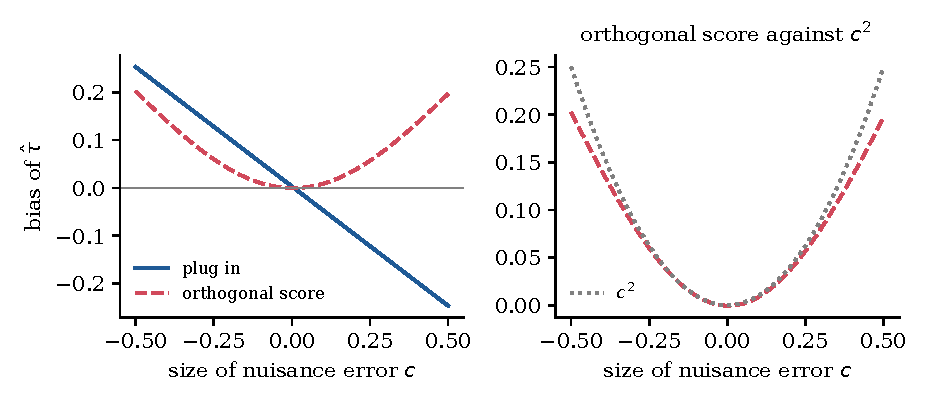
\includegraphics[width=\linewidth]{orth_bias.pdf}
\caption{Error of the plug in and orthogonal estimators of $\tau$ in one sample of 200,000 observations when the nuisance functions are perturbed by $c\,x$. Left: both estimators. Right: the orthogonal error, with the curve $c^2$ for comparison.}
\label{fig:orthbias}
\end{figure}



\section{The main theorem and what it assumes}\label{sec:dml:thm}

Software returns an estimate and an interval, and the interval is a claim about coverage. The theorem behind that claim has hypotheses the analyst cannot inspect.

\begin{theorem}[Chernozhukov and coauthors, 2018, partially linear model]\label{dml:thm:main}
Let $(Y_i, T_i, X_i)$, $i = 1, \dots, n$, be independent draws from \eqref{eq:plm1} and \eqref{eq:plm2}, cross fitted with $K$ folds of equal size\index{double machine learning!main theorem|textbf}, and suppose that
\begin{enumerate}[label=(\roman*),leftmargin=*,itemsep=1pt,topsep=2pt]
\item (moments) $\E(\varepsilon^2 \mid T, X) \le \bar\sigma^2$ and $\E(\nu^2 \mid X) \le \bar\sigma^2$ for a constant $\bar\sigma$, and $\E(\nu^2\varepsilon^2) > 0$;
\item (overlap) $J_0 = \E\nu^2 = \E\,\mathrm{Var}(T \mid X) > 0$;
\item (cross fitting) $K$ is fixed, and the fits $\hat\ell^{(-k)}$ and $\hat m^{(-k)}$ use only observations outside fold $k$;
\item (consistency) $\|\delta_m\| + \|\delta_\ell\| = o_p(1)$ for the fits of every fold;
\item (rate) $\|\delta_m\|\bigl(\|\delta_m\| + \|\delta_\ell\|\bigr) = o_p(n^{-1/2})$ for the fits of every fold.
\end{enumerate}
Then the pooled estimator \eqref{eq:dml:ratio} satisfies $\sqrt{n}(\hat\tau - \tau_0) \Rightarrow N(0, \sigma^2)$\index{asymptotic normality|textbf} with
\[
\sigma^2 = \frac{\E(\nu^2\varepsilon^2)}{J_0^2},
\]
and so does the fold wise estimator DML1.
\end{theorem}

\begin{proof}
By Lemma~\ref{dml:lem:exact}, $\sqrt{n}(\hat\tau - \tau_0) = (\sqrt{n}S_n + \sqrt{n}C_n + \sqrt{n}B_n)/\hat J_n$, and we take the pieces in turn. The $\nu_i\varepsilon_i$ are independent with mean zero and variance $\E(\nu^2\varepsilon^2) \le \bar\sigma^2 J_0$, so the central limit theorem gives $\sqrt{n}S_n \Rightarrow N(0, \E\nu^2\varepsilon^2)$.

Fix a fold $k$ and condition on its fit, with errors $\delta_m$ and $\delta_\ell$. The summands of $C_n$ in this fold are independent with mean zero. Because $\nu$ is a function of $(T, X)$, $\E(\nu\varepsilon \mid X) = 0$, and the second moment of a summand given $X$ is $(\tau_0\delta_m - \delta_\ell)^2\E(\nu^2 \mid X) + \delta_m^2\E(\varepsilon^2 \mid X) \le \bar\sigma^2\{(\tau_0\delta_m - \delta_\ell)^2 + \delta_m^2\}$. The conditional variance of $\sqrt{n}$ times the fold's part of $C_n$ is therefore at most $\bar\sigma^2(\|\tau_0\delta_m - \delta_\ell\|^2 + \|\delta_m\|^2)$, which is $o_p(1)$ by (iv), and Chebyshev's inequality given the fit makes that part $o_p(1)$.

For $B_n$, the Cauchy and Schwarz inequality\index{Cauchy Schwarz inequality|textbf} gives $\E|\delta_m\delta_\ell - \tau_0\delta_m^2| \le \max(1, |\tau_0|)\,\|\delta_m\|(\|\delta_m\| + \|\delta_\ell\|)$. By (v), the conditional absolute mean of the fold's part of $\sqrt{n}B_n$ is $o_p(1)$, so Markov's inequality makes it $o_p(1)$.

Finally $\hat J_n = n^{-1}\sum_i\nu_i^2 - 2n^{-1}\sum_i\nu_i\delta_{m,i} + n^{-1}\sum_i\delta_{m,i}^2$. The first term tends to $J_0$ by the law of large numbers\index{law of large numbers|textbf}. The third has conditional mean $\|\delta_m\|^2$ and tends to zero. The second has conditional mean zero and conditional variance at most $4\bar\sigma^2\|\delta_m\|^2/n$ in each fold. So $\hat J_n \to J_0 > 0$ in probability, and Slutsky's lemma gives the limit. Since $K$ is fixed, the sums over folds are finite sums of $o_p(1)$ terms. The same steps inside each fold show that every fold estimate is asymptotically normal with variance $\sigma^2$ at the scale $\sqrt{n/K}$. The leading terms use disjoint observations and are independent, so the average of the $K$ fold estimates has the same limit as the pooled one.
\end{proof}

This convergence is pointwise, for one distribution. Chernozhukov and coauthors prove uniform convergence for general orthogonal scores over classes with fixed constants, including a lower bound on $J_0$. Proposition~\ref{crit:prop:dufour} in Chapter~\ref{ch:critique} treats overlap failure outside that class.

The rate condition\index{rate condition|textbf} has the shape $\|\delta_m\|\{\|\delta_m\| + \|\delta_\ell\|\}$ and not the bare product $\|\delta_m\|\|\delta_\ell\|$. The square is the own square channel of Corollary~\ref{dml:cor:channels}. It asks the treatment nuisance to be better than $n^{-1/4}$\index{fourth root rate|textbf} on its own, whatever the outcome nuisance does, since $\|\delta_m\|^2 \le \|\delta_m\|(\|\delta_m\| + \|\delta_\ell\|) = o_p(n^{-1/2})$. The outcome nuisance may be slower than $n^{-1/4}$ if the treatment nuisance is faster (Exercise~\ref{ex:ch04:4}); the roles do not reverse, and Exercise~\ref{ex:ch04:8} shows why. At $n = 9{,}915$, the size of the 401(k) sample, $n^{-1/4}$ is 0.100 and $n^{-1/2}$ is 0.0100. The rate is an asymptotic statement, and numbers like these fix a scale and nothing more. The condition is sufficient and can be wasteful: what enters the bias is the inner product $\langle\delta_m, \delta_\ell - \tau_0\delta_m\rangle$, which the product of norms bounds by the Cauchy and Schwarz inequality, and Chapter~\ref{ch:critique} replaces the bound by the exact quantity (Theorem~\ref{crit:thm:sharp}).

Under slightly stronger moment conditions on the nuisance errors, Chernozhukov and coauthors show that the sandwich standard error of step 5 consistently estimates $\sigma/\sqrt{n}$. The confidence interval\index{confidence interval|textbf} $\hat\tau \pm 1.96\,\widehat{\mathrm{se}}$ then has asymptotic coverage 0.95, the claim the rest of the book tests.

With clustered observations, such as households sharing an employer or repeated observations of one unit, form folds from whole clusters so that no fit trains on observations dependent on those used for evaluation. Sum the scores within clusters before squaring for the standard error; the number of clusters replaces $n$. Chiang, Kato, Ma and Sasaki (2022) give the theory, including clustering in more than one dimension.

Conditions (iv) and (v) cannot be checked from the data, since they are statements about the distance between fitted and true functions. 

\section{The interactive model, AIPW and the estimand}\label{sec:dml:wate}

Suppose the retirement plan helps high income households more than low income ones. The partially linear model, with one $\tau$ for everybody, is then misspecified, and a DML routine will still return a number. The number is an average\index{estimand!of the partially linear model|textbf}\index{partially linear model!estimand of|textbf}, each household's effect weighted by the variance of its treatment given its covariates.

\begin{proposition}[The partially linear estimand]\label{dml:prop:wate}
Suppose $Y = \tau(X)T + g(X) + \varepsilon$ with $\E(\varepsilon \mid T, X) = 0$, so that the effect varies with $X$. Let $\tau_*$\index{partially linear model!estimand of} solve the population Robinson moment condition\index{moment condition|textbf} $\E\,\psi(W; \tau, \ell, m) = 0$ at $\ell(X) = \E(Y \mid X)$ and $m(X) = \E(T \mid X)$, and assume $\E\varepsilon^2 < \infty$, $0 < \E\,\mathrm{Var}(T \mid X) < \infty$ and $\E|\tau(X)\,\mathrm{Var}(T \mid X)| < \infty$. Then
\[
\tau_* = \frac{\E\bigl[\mathrm{Var}(T \mid X)\,\tau(X)\bigr]}{\E\bigl[\mathrm{Var}(T \mid X)\bigr]}.
\]
If also $\E|\tau(X)| < \infty$, then $\tau_* - \ATE = \Cov\bigl(\tau(X), \mathrm{Var}(T \mid X)\bigr)\big/\E\,\mathrm{Var}(T \mid X)$. For a binary treatment the weight is $\mathrm{Var}(T \mid X) = e(X)\{1 - e(X)\}$.
\end{proposition}

\begin{proof}
Since $\ell(X) = \tau(X)m(X) + g(X)$, the outcome residual is $V_Y = Y - \ell(X) = \tau(X)V_T + \varepsilon$ with $V_T = T - m(X)$. The moment condition gives $\tau_* = \E[V_TV_Y]/\E[V_T^2]$. Now $\E[V_TV_Y] = \E[\tau(X)V_T^2] + \E[V_T\varepsilon] = \E[\tau(X)\,\mathrm{Var}(T \mid X)]$, because $\E(\varepsilon \mid T, X) = 0$ and the tower property apply, and $\E V_T^2 = \E\,\mathrm{Var}(T \mid X)$. The second display follows from $\E[\tau\,\mathrm{Var}] = \E\tau\,\E\mathrm{Var} + \Cov(\tau, \mathrm{Var})$.
\end{proof}

The discrepancy is a property of the moment condition, so neither more data, cross fitting nor a different learner removes it. This is the classical weighting problem for regression adjustment (Angrist 1998; Aronow and Samii 2016; S{\l}oczy\'nski 2022; Vansteelandt and Daniel 2014).

Whether the weighting is a defect depends on the question. The households that receive least weight are those whose treatment is most nearly determined by their covariates, about which an observational study has least to say. Crump, Hotz, Imbens and Mitnik (2009) argue for trimming to the subpopulation with adequate overlap, because the variance of any estimator of the unweighted average effect is dominated by the region where the propensity is near zero or one. Li, Morgan and Zaslavsky (2018) develop overlap weighting\index{overlap weighting|textbf}, whose weight $e(1 - e)$ is exactly the one above, on variance grounds. The estimand $\tau_*$ is defensible. The difficulty is that a DML routine arrives at it silently: an analyst who chooses overlap weighting knows which population she describes, and an analyst who calls a routine for the average effect has been handed a different one.

The interval such a routine reports is still asymptotically valid, but for $\tau_*$. For a binary treatment and a bounded $\tau(X)$, write $Y - \ell(X) = \tau_*\nu + r$ with $r = \varepsilon + \{\tau(X) - \tau_*\}\nu$. Then $\E(r \mid X) = 0$, and $\E(\nu r) = 0$ by the definition of $\tau_*$, so the proof of Theorem~\ref{dml:thm:main} goes through with $r$ in place of $\varepsilon$ (only the bound on the second moments in $C_n$ becomes cruder: $\E(\nu r \mid X)$ no longer vanishes, and $(u + v)^2 \le 2u^2 + 2v^2$ absorbs the cross term) and gives $\sqrt{n}(\hat\tau - \tau_*) \Rightarrow N\bigl(0, \E(\nu^2 r^2)/J_0^2\bigr)$. The residuals $\hat\varepsilon_i$ of step 5 estimate the $r_i$, so the sandwich standard error is aimed at this variance. Coverage survives; the target is what moved.

The arithmetic is simple enough to do by hand. Take eight strata of equal size, with propensities spaced evenly from 0.06 to 0.50 and stratum effects spaced evenly from 2.0 down to 0.0, so that the effect is largest where overlap is weakest. The average effect is 1.0. Table~\ref{tab:dml:strata} lists the weights $w_g = \pi_g(1 - \pi_g)$ and the weighted effects. The weights sum to 1.4469 and the weighted effects to 1.1150, and since the strata are equal the common stratum probability cancels, so $\tau_* = 1.1150/1.4469 = 0.7706$. The partially linear score answers 0.7706 to a question posed about an average effect of 1.0, a shortfall of 23 percent that no learner, sample size or number of folds can close. The stratum with the largest effect, 2.0, receives 3.9 percent of the weight, and the stratum with no effect receives 17.3 percent. Section~\ref{sec:crit:repair} returns to these strata.

\begin{table}[ht]
\centering
\caption{Eight strata of equal size. The propensities $\pi_g$ are spaced evenly from 0.06 to 0.50 and the effects $\tau_g$ evenly from 2.0 to 0.0, so the average effect is 1.0000. The totals add the unrounded entries, and $\tau_* = 1.1150/1.4469 = 0.7706$.}
\label{tab:dml:strata}
\small
\begin{tabular}{rrrrr}
\toprule
Stratum $g$ & $\pi_g$ & $\tau_g$ & $w_g = \pi_g(1 - \pi_g)$ & $w_g\tau_g$ \\
\midrule
1 & 0.0600 & 2.0000 & 0.0564 & 0.1128 \\
2 & 0.1229 & 1.7143 & 0.1078 & 0.1847 \\
3 & 0.1857 & 1.4286 & 0.1512 & 0.2160 \\
4 & 0.2486 & 1.1429 & 0.1868 & 0.2135 \\
5 & 0.3114 & 0.8571 & 0.2144 & 0.1838 \\
6 & 0.3743 & 0.5714 & 0.2342 & 0.1338 \\
7 & 0.4371 & 0.2857 & 0.2460 & 0.0703 \\
8 & 0.5000 & 0.0000 & 0.2500 & 0.0000 \\
\midrule
Total & & & 1.4469 & 1.1150 \\
\bottomrule
\end{tabular}
\end{table}

When the effect varies, DML can target the average effect directly by using the interactive regression model\index{interactive regression model|textbf},
\[
Y = \mu_T(X) + \varepsilon, \qquad \E(\varepsilon \mid X, T) = 0,
\]
with no restriction on how $\mu_1$ and $\mu_0$ differ. The target is $\tau = \E\{\mu_1(X) - \mu_0(X)\}$, and for a binary treatment the orthogonal score is the augmented inverse probability weighted (AIPW)\index{augmented inverse probability weighting|textbf}\index{AIPW|see{augmented inverse probability weighting}} score of Robins, Rotnitzky and Zhao (1994),
\begin{equation}
\psi = \mu_1(X) - \mu_0(X) + \frac{T\{Y - \mu_1(X)\}}{e(X)} - \frac{(1-T)\{Y - \mu_0(X)\}}{1 - e(X)} - \tau,
\label{eq:aipw}
\end{equation}
where $\mu_t(x) = \E(Y \mid X = x, T = t)$. It is doubly robust\index{double robustness!and the augmented estimator|textbf}: it has mean zero if either the outcome regressions or the propensity score\index{propensity score} are correct. At nuisance values $(\hat\mu_1, \hat\mu_0, \hat e)$ and the true $\tau$ its mean is exactly
\[
\E\Bigl[(\hat e - e)\Bigl\{\frac{\hat\mu_1 - \mu_1}{\hat e} + \frac{\hat\mu_0 - \mu_0}{1 - \hat e}\Bigr\}\Bigr],
\]
a sum of two products of the propensity error with the outcome errors (Exercise~\ref{ex:ch04:10}). Every term is a product, so no first order term remains. Cross fitting proceeds as before, with nuisances $\mu_1$, $\mu_0$ and $e$, and the rate condition becomes
\[
\|\hat\mu_t - \mu_t\|\,\|\hat e - e\| = o_p(n^{-1/2}), \qquad t = 0, 1,
\]
together with overlap\index{overlap}, which enters the constant through the inverse of the estimated propensity and of one minus it. Overlap matters more directly here than for the partially linear score, since the score divides by $e(X)$ and $1 - e(X)$. In practice propensity estimates are clipped, typically to $[0.01, 0.99]$. Clipping bounds the weights and leaves the target where it was, but where the true propensity lies outside the clipping range the clipped $\hat e$ cannot converge to it, the propensity factor of the remainder above stops shrinking, and the outcome regressions must carry the whole burden (Exercise~\ref{ex:ch04:10}). Trimming, which drops households, is what changes the target (Chapter~\ref{ch:ipw}). The AIPW score is the efficient influence function of the average effect, so under this rate condition, with each nuisance estimate consistent and the true and fitted propensities bounded away from zero and one, the cross fitted estimator attains the semiparametric efficiency bound of Hahn (1998).

Applications often ask for the average effect on the treated\index{effect on the treated|textbf}\index{average effect on the treated|see{effect on the treated}}\index{ATT|see{effect on the treated}}, $\tau_T = \E\{\mu_1(X) - \mu_0(X) \mid T = 1\}$, as Chapter~\ref{ch:k401} does for the trainees of the LaLonde data. Its efficient score\index{augmented inverse probability weighting!for the effect on the treated|textbf}\index{double machine learning!for the effect on the treated|textbf} needs only $\mu_0$ and $e$, and the weight on the controls is the odds of treatment. With $p = \Prob(T = 1)$,
\begin{equation}
\psi_T = \frac{1}{p}\Bigl[T\{Y - \mu_0(X) - \tau_T\} - (1 - T)\,\frac{e(X)}{1 - e(X)}\{Y - \mu_0(X)\}\Bigr].
\label{eq:aipw:att}
\end{equation}
It is doubly robust in the same way: at nuisance values $(\hat\mu_0, \hat e)$ and the true $\tau_T$ its mean is $p^{-1}\E[(\hat\mu_0 - \mu_0)(\hat e - e)/(1 - \hat e)]$, again a product of the two errors, so it vanishes if either is right (Exercises~\ref{ex:chlalonde:3} and~\ref{ex:chk401:3} derive it and put it to work). Overlap enters only through $e(X) < 1$: every treated unit needs comparable controls, but a control with no comparable treated unit simply receives weight near zero.

The same partialling out extends to conditional effects. Nie and Wager's (2021) R learner\index{R learner|textbf} writes $Y - \ell(X) = \tau(X)\{T - m(X)\} + \varepsilon$ and chooses $\tau(\cdot)$ to minimize $\E\bigl[\{Y - \ell(X) - \tau(X)(T - m(X))\}^2\bigr]$ over functions, with cross fitted $\hat\ell$ and $\hat m$ plugged in and any regularized learner fitting $\tau(\cdot)$. Its error inherits the product structure above. The R loss is a useful objective; it is not a posterior, and Chapter~\ref{ch:bart} fits the response surface directly.

\section{What DML delivers in practice}\label{sec:dml:practice}

An applied economist with a large survey and a hundred controls used to pick variables by hand, run least squares and report the interval as if the selection had not happened. DML gave her a principled replacement\index{double machine learning!in practice|textbf}: an estimator that is $\sqrt{n}$ consistent and asymptotically normal under conditions far weaker than parametric models need. It is also cheap. A cross fitted lasso at $n = 300$ and $p = 400$ takes 1.0 seconds with five folds, averaged over ten simulated data sets on one processor core, in a timing run of our own (Chapter~\ref{ch:critique}). It needs no model for the nuisance functions and no convergence diagnostics, it accepts any learner, and anyone who can call a package can run it. DoubleML\index{software!DoubleML|textbf} and EconML\index{software!EconML|textbf} implement the estimators of this chapter in Python, and DoubleML also has an interface in R; in both the analyst makes the choices of the box in Section~\ref{sec:dml:cf}. Chapter~\ref{ch:critique} quotes simulations and real data comparisons from our working paper ``Orthogonality is not enough'' (Polson and Sokolov 2026b). Cheapness belongs to the learner as much as to the template: in the same run the score with a horseshoe posterior mean as the nuisance learner (Chapter~\ref{ch:horseshoe}) takes 19.1 seconds at five folds.

The lasso can meet the rate condition under sparsity, random forests under smoothness and neural networks under compositional structure, but whether a given data set has the structure is something the data do not say.

The simulations of that working paper, which we reran with our own code and ten times the replications, show both sides of the method. The baseline design has $n = 300$ and $p = 400$ independent standard normal covariates, of which the first $s$ enter the treatment equation with coefficient one and the outcome equation with coefficients drawn uniformly from 0.8 to 1.2 afresh in each replication, a true effect $\tau_0 = 1$, standard normal treatment noise, normal outcome noise with standard deviation 0.948, and cross validated lasso learners for both nuisance functions. A fourth design keeps $s = 15$ and weakens overlap by lowering the treatment noise standard deviation to 0.3. Each design has 5,000 replications, and Table~\ref{tab:dml:sims} reports the bias of the estimate and the coverage\index{coverage|textbf} of the nominal 95 percent interval\index{coverage!of DML intervals|textbf}. With five folds, coverage falls from 0.917 at $s = 5$ to 0.734 at $s = 30$, and to 0.557 under weak overlap, where the bias is 0.317. At $n = 1200$, $p = 200$ and $s = 15$ it recovers to 0.934, with bias 0.007. Moving from five folds to two lowers coverage in every design, from 0.826 to 0.694 at $s = 15$ and from 0.734 to 0.450 at $s = 30$, while the reported standard error hardly moves (from 0.0523 to 0.0513 at $s = 15$). Two folds also cut each fit's training share from 80 to 50 percent, so part of the loss is worse fits, and the cleaner reading is that the reported error does not respond to the fold count. The finding belongs to this design. In the 401(k) data, with $n = 9{,}915$, the partition to partition spread is small beside the standard error (Section~\ref{sec:dml:k401}).

\begin{table}[ht]
\centering
\caption{DML with cross validated lasso learners in the designs of Section~\ref{sec:dml:practice}: $n = 300$, $p = 400$, $\tau_0 = 1$ and 5,000 replications a design. The weak overlap design has $s = 15$ and treatment noise standard deviation 0.3. Bias is that of the estimate from one partition into five folds. The coverage columns are for nominal 95 percent intervals from one partition into five folds, one partition into two folds, and the median over 20 partitions into five folds with the standard error of step 6 of the algorithm.}
\label{tab:dml:sims}
\small
\begin{tabular}{lrrrr}
\toprule
Design & Bias & \multicolumn{3}{c}{Coverage} \\
\cmidrule(lr){3-5}
 & $K = 5$ & $K = 5$ & $K = 2$ & median, $S = 20$ \\
\midrule
$s = 5$ & 0.017 & 0.917 & 0.865 & 0.936 \\
$s = 15$ & 0.037 & 0.826 & 0.694 & 0.870 \\
$s = 30$ & 0.050 & 0.734 & 0.450 & 0.820 \\
weak overlap, $s = 15$ & 0.317 & 0.557 & 0.235 & 0.603 \\
\bottomrule
\end{tabular}
\end{table}

Selection with a theory driven penalty does better where its sparsity assumption holds. At $s = 5$ post double selection\index{double selection} (Belloni, Chernozhukov and Hansen 2014) covers 0.950 against 0.917 for DML, and at $s = 15$ it collapses to a coverage of 0.010, because the penalty is calibrated to a sparsity the design does not have. The median over 20 repeated splits\index{cross fitting!repeated splits|textbf} covered better than a single split in all four designs (the last column of Table~\ref{tab:dml:sims}), at 3 to 11 percent more width. DML is one good tool among several where sparsity holds, and the choice among them is itself something the data may not settle.

What DML does not deliver is a posterior. It gives a point estimate and an interval for one functional, with a frequentist guarantee that holds as $n$ grows. It says nothing about the conditional effect at a particular $x$, the effect on the treated\index{effect on the treated}, quantile effects or the probability that treatment helped a given individual, unless each is separately derived. Nor does it say how much to trust the answer at the sample size in hand. Chapters~\ref{ch:horseshoe} and~\ref{ch:k401} report posteriors for the models of this chapter.

\section{The 401(k) story}\label{sec:dml:k401}

A 401(k) plan\index{401(k) plan|textbf} is an employer sponsored, tax advantaged retirement savings account, and a worker is eligible if her employer offers one. Whether eligibility raises savings, or only marks people who would have saved anyway, was argued through the 1990s. Poterba, Venti and Wise (1995) took the first view: conditional on income and a few other characteristics, eligibility is close to randomly assigned, because workers chose jobs mainly for their wages and other features. If that holds, adjusting for the observed covariates identifies the effect of eligibility on savings, which is the unconfoundedness that DML assumes.

The data are the 1991 wave of the Survey of Income and Program Participation\index{401(k) plan!story of the data|textbf}: 9,915 households, 37 percent of them eligible. The outcome is net total financial assets in thousands of dollars. The nine characteristics of Section~\ref{sec:dml:question} are expanded into 54 standardized terms for the lasso, namely the characteristics, their squares and all pairwise interactions (the squares of the five binary characteristics repeat them, so the rank is 49).  We use five folds, the pooled estimator and the sandwich standard error of the algorithm box, with forests of 200 trees or a lasso whose penalty is chosen by cross validation.

The raw difference in means is 19.56 thousand dollars. DML with random forests as learners gives 8.59, with a 95 percent interval from 6.05 to 11.12, and DML with the lasso on the 54 term basis gives 9.52, with an interval from 6.89 to 12.14. Both are less than half the raw difference, and they differ from each other by 0.93, less than one standard error (about 1.3). Least squares with the nine characteristics entered linearly gives 5.90 and with the 54 terms 9.84.

Each figure is one random partition, and for both learners the partition reported above happens to give the lowest estimate we found. Over 20 partitions the lasso estimates run from 9.52 to 10.26, with median 9.84 and standard deviation 0.17, and over five partitions the forest estimates run from 8.59 to 9.05, with median 9.00 and standard deviation 0.21. The spread is small next to the standard error and not zero: two analysts with the same data and the same method, differing only in the seed, can report point estimates 0.7 thousand dollars apart.

The sample is large, and the treatment nuisance is the probability of eligibility given nine characteristics. A logistic regression of eligibility on the 54 terms, fitted to the full sample, gives estimated probabilities from 0.02 to 0.89, which suggests that $J_0$ is not close to zero though the lower tail is thin. This is the regime in which one expects the rate condition to be credible, and the agreement of two very different learners is what one would see if it were. It is not a test of the condition, because two learners can share a bias. Nor does it say which effect has been estimated. The posterior analysis of Chapter~\ref{ch:k401} finds the effect rising from 1.41 thousand dollars in the lowest income quintile to 20.78 in the highest, a gap of about 19 thousand dollars that a single average hides. Agreement among estimators that share a score shows that, in these data, the choice between the two learners mattered little. It does not show that the score is the right one.

\section{What DML assumes, in one list}\label{sec:dml:assume}

An analyst assessing a DML interval\index{double machine learning!assumptions|textbf} faces six questions\index{double machine learning!six questions for the analyst|textbf}. The first four are hypotheses of Theorem~\ref{dml:thm:main} or its model; the last two concern how well its limit describes the sample in hand.

\begin{enumerate}[label=(A\arabic*),leftmargin=*,itemsep=2pt]
\item \emph{Unconfoundedness.} All confounders are in $X$ and the model \eqref{eq:plm1} and \eqref{eq:plm2} holds. DML does nothing about unmeasured confounding, a limitation shared with every method in Parts II and III and addressed in later parts.
\item \emph{Overlap.} The treatment keeps variation given the covariates, $J_0 > 0$, and in the uniform theory $J_0$ stays above a constant fixed in advance. A histogram of the estimated propensities shows part of this; $\hat J_n$ is no substitute for it (Corollary~\ref{dml:cor:channels}). Proposition~\ref{crit:prop:dufour} says what no interval can do when $J_0$ is allowed to approach zero.
\item \emph{A stated estimand.} If effects differ across households, the partially linear score estimates the variance weighted average of Proposition~\ref{dml:prop:wate}, and the average effect needs the augmented score and its stronger overlap. A different target, such as the effect on the treated or the effect at a given $x$, needs a new score, a new derivation and a new run.
\item \emph{Nuisance rates.} The rate condition of Theorem~\ref{dml:thm:main}, including the square of the treatment error, holds for the chosen learners on this data set, and there is no diagnostic for it. A learner slowed by a rough regression function silently invalidates the interval. Theorem~\ref{crit:thm:sharp} writes the bias that the product bound only bounds, and Proposition~\ref{crit:prop:alignment} describes one mechanism by which the bound is attained.
\item \emph{Asymptotic normality at the sample size in hand.} The guarantee is first order. In moderate samples the second order terms, which depend on the learners, can dominate, and a heavy tailed outcome slows the central limit theorem.
\item \emph{Splitting is harmless.} Different random partitions give different estimates, and the standard error of one partition leaves out their spread. The spread vanishes at first order under Theorem~\ref{dml:thm:main} but not at the sample size in hand; Theorem~\ref{crit:thm:single} says what the standard error of a single split leaves out, and Proposition~\ref{crit:prop:cfvar} with the simulations that follow it shows how cross fitting changes the omitted part.
\end{enumerate}

\section{In practice}

\paragraph{The target.} The partially linear $\tau$ is the coefficient of $T$ in the outcome model: draw that model's parameters from their posterior and read off $\tau^{(s)}$. If the model allows $\tau(x)$ to vary, then $\tau_Q^{(s)} = \int \tau^{(s)}(x)\,Q(dx)$ for any $Q$, including the overlap\index{overlap} weighted population that the partially linear score implicitly targets when effects vary (Proposition~\ref{dml:prop:wate}).

\paragraph{What the analyst does differently.} An analyst who has read this chapter and still wants to run DML should do four things. State the estimand before choosing the model, because the partially linear score silently changes the target when effects vary (Exercise~\ref{ex:ch04:1}). Look at the distribution of the estimated propensities directly, and do not read $\hat J_n$ as a statement about overlap. Report the median and the spread of the estimate across random fold partitions, not one partition, since Table~\ref{tab:k401} depends on a seed. And treat the confidence interval as an asymptotic statement whose accuracy at the sample size in hand is unknown, since nothing in the method reports how close the normal approximation is at a given sample size. An analyst who fits the model instead reports a posterior that answers the same question and, from the same draws, the effect at any $x$ and in any subgroup.

\paragraph{Against DML.} DML with the partially linear score is a sound choice when four conditions hold together. The treatment retains substantial variation given the covariates, so that $J_0$ is bounded away from zero. The effect is plausibly homogeneous, or the variance weighted average of Proposition~\ref{dml:prop:wate} is the estimand of interest. The nuisance functions are sparse or smooth enough for the dimension that the rate condition is credible and not merely invoked. And the analyst wants one number quickly and will not make a decision that depends on the width. In the design of Section~\ref{sec:dml:practice}, DML with five folds and a cross validated lasso is at its best with 5 relevant covariates, loses coverage as their number grows to 30 or as overlap weakens, and recovers at $n = 1200$ and $p = 200$ (Table~\ref{tab:dml:sims}). What we resist is the method used as a default, without asking whether the four conditions obtain and with its interval read as a description of uncertainty. Homogeneity the partially linear score cannot diagnose, since it averages over whatever heterogeneity is present. Overlap can be diagnosed, though not by $\hat J_n$. The rate condition cannot be verified from the data. The fourth condition is a statement about the analyst. When the first three fail, or when more than one number is wanted, the chapters that follow ask what a model based analysis offers and what it costs.

\section*{Notes}

Double machine learning is due to Chernozhukov, Chetverikov, Demirer, Duflo, Hansen, Newey and Robins (2018), who use the 401(k) question as their leading illustration. The exact decomposition of Section~\ref{sec:dml:exact} and its two channel form come from Polson and Sokolov (2026b), the working paper ``Orthogonality is not enough''. Chernozhukov, Escanciano, Ichimura, Newey and Robins (2022b) construct locally robust scores for functionals beyond those treated here.

\begin{exercises}
\item\label{ex:ch04:1} Show that when $\tau(x)$ varies but the partially linear model is fitted, the DML estimand is $\E\{\nu^2 \tau(X)\}/\E\nu^2$, an overlap weighted average of conditional effects.
\item\label{ex:ch04:2} Verify that the AIPW score \eqref{eq:aipw} is Neyman orthogonal with respect to both $\mu_t$ and $e$.
\item\label{ex:ch04:3} Prove the double robustness of \eqref{eq:aipw}: show its mean is zero if either $\mu_t$ or $e$ is correct.
\item\label{ex:ch04:4} Give an example in which the rate condition of Theorem~\ref{dml:thm:main} holds although one nuisance is estimated at a rate slower than $n^{-1/4}$.
\item\label{ex:ch04:5} Simulate the partially linear model of Section~\ref{sec:ricsim}: $n = 200$ observations, $p = 50$ independent standard normal covariates, five of which have coefficient one in both the treatment and the outcome equation, independent standard normal $\nu$ and $\varepsilon$, and $\tau = 1$. Run DML with lasso nuisance learners and five folds on ten different random splits of one data set and report the spread of the estimates. Compare with the posterior standard deviation of the coupled horseshoe of Chapter~\ref{ch:horseshoe} on the same data set.
\item\label{ex:ch04:6} Let $X_1, \ldots, X_{50}$ be independent $N(0,1)$, $T = X_1 + \cdots + X_5 + \nu$ and $Y = \tau T + X_1 + \cdots + X_5 + \varepsilon$, with $\nu$ and $\varepsilon$ standard normal and $\tau = 1$. Let $\tau_\lambda$ be the coefficient of $T$ in the lasso of $Y$ on $(T, X)$ with objective $(2n)^{-1}\|Y - T\tau - Xb\|^2 + \lambda\|b\|_1$, so that $T$ is not penalized. Show that as $n$ grows with $\lambda$ fixed, $\tau_\lambda - \tau$ tends to $5\lambda$ for $\lambda \le 1/6$, and find the limit for larger $\lambda$.
\item\label{ex:ch04:7} Derive Lemma~\ref{dml:lem:exact} without looking at its proof: start from $\hat V_{T,i} = \nu_i - \delta_{m,i}$ and $\hat V_{Y,i} = \tau_0\nu_i + \varepsilon_i - \delta_{\ell,i}$ and show that the numerator of $\hat\tau - \tau_0$ is $\sum_i \hat V_{T,i}(\hat V_{Y,i} - \tau_0\hat V_{T,i})$. State and prove the version for the ratio computed inside one fold, and use the two to show that DML2 is the average of the fold ratios weighted by their denominators.
\item\label{ex:ch04:8} Suppose the outcome nuisance is exact, $\hat\ell = \ell$, so that $\|\delta_m\|\,\|\delta_\ell\| = 0$. Show that the bias of Corollary~\ref{dml:cor:channels} is $-\tau_0\|\delta_m\|^2/(J_0 + \|\delta_m\|^2)$, and conclude that $\|\delta_m\|\,\|\delta_\ell\| = o_p(n^{-1/2})$ alone does not give the central limit theorem. For which choices of $\hat\ell$ do the two channels cancel exactly?
\item\label{ex:ch04:9} Reproduce the numbers of Table~\ref{tab:dml:strata}: the weights, the weighted effects, their totals and $\tau_*$. Check that $\tau_* - 1$ equals the covariance of $\tau_g$ and $w_g$ over the strata divided by the mean of $w_g$. Then reverse the order of the stratum effects, so that the largest effect sits where overlap is best, and find the new $\tau_*$.
\item\label{ex:ch04:10} Show that the mean of the AIPW score at the true $\tau$ and nuisance values $(\hat\mu_1, \hat\mu_0, \hat e)$ equals $\E\bigl[(\hat e - e)\{(\hat\mu_1 - \mu_1)/\hat e + (\hat\mu_0 - \mu_0)/(1 - \hat e)\}\bigr]$, and deduce that the score is Neyman orthogonal in $(\mu_1, \mu_0, e)$. Where do overlap and the clipping of $\hat e$ enter a bound on this remainder?
\item\label{ex:ch04:11} Using Table~\ref{tab:dml:six}, compute the two fold estimates, DML1, DML2 and the weights that DML2 gives to the folds. Then keep the six pairs of residuals but regroup the observations into the folds $\{1, 4, 5\}$ and $\{2, 3, 6\}$, and recompute both estimators. Which one changes, and why?
\end{exercises}

\chapter{The Inverse Weighting Lineage}\label{ch:ipw}

\begin{tcolorbox}[colback=gray!6,colframe=gray!50,title=In brief,fonttitle=\normalfont\itshape,coltitle=black,colbacktitle=gray!15,boxrule=0.4pt,arc=1pt]
From Horvitz and Thompson to the augmented score, every improvement on inverse weighting has moved weight off the weights and onto an outcome model. Weights explode under weak overlap, trimming changes the estimand, and Basu's elephants show that design unbiasedness says little about the sample in hand. In the Robins, Ritov and Wasserman example a prior that ignores the known propensity is off by 0.157, a prior coupled to it matches Horvitz and Thompson, and a hierarchical estimator drops the $1/p$ factor from the Horvitz Thompson and H\'ajek variances.
\end{tcolorbox}

Double machine learning descends from a long line of estimators that reweight observed outcomes by the inverse of their probability of being observed\index{inverse probability weighting|textbf}\index{IPW|see{inverse probability weighting}}\index{inverse propensity weighting|see{inverse probability weighting}}\index{inverse weighting|see{inverse probability weighting}}. The line runs from Horvitz and Thompson\index{Horvitz Thompson estimator}'s 1952 survey sampling estimator, through the 1990s work of Robins and his collaborators on missing data and causal inference, to the augmented score of Chapter~\ref{ch:dml}. The lineage clarifies what DML inherits and what it cannot escape.

\section{Horvitz and Thompson}

In survey sampling\index{survey sampling|textbf} a finite population of $N$ units has values $y_1, \ldots, y_N$. A sample is drawn with known inclusion probabilities\index{inclusion probability|textbf} $\pi_1, \ldots, \pi_N$. The Horvitz Thompson estimator\index{Horvitz Thompson estimator|textbf} of the population total is
\[
\hat Y_{\mathrm{HT}} = \sum_{i \in \text{sample}} \frac{y_i}{\pi_i}.
\]

\begin{proposition}
$\hat Y_{\mathrm{HT}}$ is unbiased\index{Horvitz Thompson estimator!unbiasedness|textbf} for $\sum_{i=1}^N y_i$ over the sampling design, whatever the values $y_i$, provided every $\pi_i > 0$.
\end{proposition}

\begin{proof}
Write $R_i$ for the indicator that unit $i$ is sampled. Then $\hat Y_{\mathrm{HT}} = \sum_{i=1}^N R_i y_i / \pi_i$ and $\E R_i = \pi_i$.
\end{proof}

No model for the $y_i$ is needed, but small $\pi_i$ give sampled units enormous weights and high variance.

The variance depends on the design through the joint inclusion probabilities $\pi_{ij} = \Prob(R_i = R_j = 1)$, with $\pi_{ii} = \pi_i$:
\[
\mathrm{Var}(\hat Y_{\mathrm{HT}}) = \sum_{i=1}^N\sum_{j=1}^N (\pi_{ij} - \pi_i\pi_j)\frac{y_iy_j}{\pi_i\pi_j}.
\]
Under independent Bernoulli sampling $\pi_{ij} = \pi_i\pi_j$ for $i \neq j$ and the variance reduces to $\sum_i (1 - \pi_i)y_i^2/\pi_i$, the case of Section~\ref{sec:weak}; fixed size designs keep the cross terms. An unbiased estimate of this variance needs every $\pi_{ij} > 0$, a condition on pairs that unbiasedness of the total does not require.

The causal analogue replaces sampling by treatment. A unit's $Y(1)$ is observed with probability $e(X)$. The inverse probability weighted estimator\index{Horvitz Thompson estimator} of the average treatment effect is
\begin{equation}
\hat\tau_{\mathrm{IPW}} = \frac{1}{n}\sum_{i=1}^n \left\{\frac{T_i Y_i}{e(X_i)} - \frac{(1-T_i)Y_i}{1 - e(X_i)}\right\},
\label{eq:ipw}
\end{equation}
unbiased when $e$ is known, $0 < e(x) < 1$ for all $x$, and ignorability\index{ignorability} holds.

\section{Basu's elephants}

In a 1971 essay Basu told a story\index{Basu elephants@Basu's elephants|textbf}\index{paradoxes|seealso{Basu's elephants; inhalation paradox; Simpson's paradox; Stein's paradox; weak paradoxes}} that has become the standard objection to design based inference\index{design based inference|textbf}. A circus owner plans to ship his 50 elephants. He knows from three years ago that an elephant called Sambo was of average weight, and plans to weigh Sambo and multiply by 50.

The circus statistician is horrified and insists on a sampling design: Sambo with probability $99/100$ and each of the other 49 elephants with probability $1/4900$. Sambo is selected, and the Horvitz Thompson estimate is Sambo's weight divided by $99/100$, about one elephant's weight as the estimate of the total for fifty. Had the largest elephant, Jumbo, been selected, the answer would have been Jumbo's weight times 4,900. The statistician is sacked and becomes a teacher of statistics.

Basu's point is that the Horvitz Thompson estimator is unbiased over a design no sensible person cares about, and absurd for the data in hand. The owner's model, that Sambo is typical, contains all the useful information; the design probabilities contain almost none. The causal analogue is direct: a treated unit with propensity $e(x) = 0.01$ receives weight 100 in \eqref{eq:ipw}, and if its outcome is unusual the estimate moves accordingly.

\section{The H\'ajek correction and stabilized weights}\label{sec:hajek}

H\'ajek's ratio estimator\index{Hajek estimator@H\'ajek estimator|textbf} normalizes the weights:
\[
\hat\mu_{1,\mathrm{H}} = \frac{\sum_i T_i Y_i / e(X_i)}{\sum_i T_i / e(X_i)}.
\]
It is no longer exactly unbiased, but it shifts by exactly any constant added to all outcomes, and its variance is usually much smaller. In causal inference it is called the normalized, or self normalized, inverse weighting estimator.

Horvitz and Thompson divide $\sum_i T_iY_i/e(X_i)$ by $n$; H\'ajek divides by the realized weight sum $\sum_i T_i/e(X_i)$, whose expectation is $n$ but which a few small propensities can push far from it. If this sum is thirty percent above $n$, the Horvitz Thompson estimate is inflated by thirty percent relative to H\'ajek. Stabilized weights\index{stabilized weights|textbf}\index{inverse probability weighting!stabilized|textbf}, used in marginal structural models, multiply each inverse weight by the marginal probability of the observed treatment. Their expected weight is one, but their realized sum remains random. Within an arm the multiplier is a constant that cancels from a normalized mean, adding nothing to H\'ajek. Neither device bounds the weights under poor overlap.



\section{Weights under weak overlap}

How bad can weighting\index{inverse probability weighting!under weak overlap|textbf} be? We simulate $n = 1000$ units with $X \sim N(0,1)$, propensity $e(x) = \expit(sx)$, and outcome $Y = X + T + \varepsilon$ with $\varepsilon \sim N(0,1)$, at slopes $s = 0.5, 1, \ldots, 4$ with 300 replications each, weighting by the true propensity. As the selection slope $s$ grows, overlap deteriorates\index{weak overlap|textbf}\index{overlap!weak|textbf}: some treated units have tiny propensities and some controls propensities close to one.

\begin{figure}[ht]
\centering
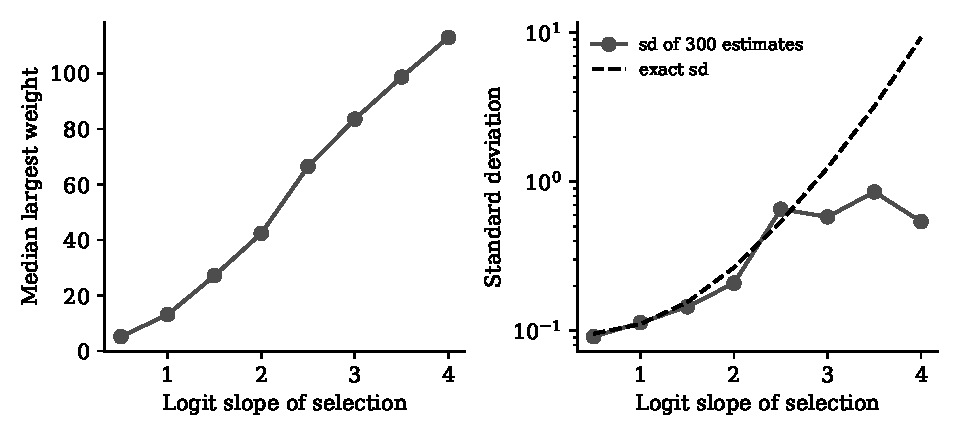
\includegraphics[width=\linewidth]{ipw_var.pdf}
\caption{Inverse weighting as overlap deteriorates, 300 replications per slope. Left: median of the largest weight in the sample. Right: standard deviation of the 300 IPW estimates at each slope (dots) and the exact standard deviation (dashed), on a log scale; the replications fall below it beyond $s = 2.5$.}
\label{fig:ipw}
\end{figure}

In Figure~\ref{fig:ipw} the median largest weight grows from about 5 at $s = 0.5$ to about 113 at $s = 4$. The standard deviation of the 300 estimates grows erratically from 0.09 to between 0.5 and 0.9. The exact variance of \eqref{eq:ipw} is $\{4 + \exp(s^2/2)(2s^2 - 2s + 5)\}/n$ (Exercise~\ref{ex:ch05:3}), giving standard deviations of 0.095 at $s = 0.5$, 0.27 at $s = 2$, 1.2 at $s = 3$ and 9.3 at $s = 4$. The replications agree within about a fifth up to $s = 2.5$, but fall two, four and seventeen times below the exact values at $s = 3$, 3.5 and 4: they seldom contain the rare units with enormous weights that dominate the variance. Where the estimator is worst, the replications understate its variance, and a confidence interval computed from one data set is not to be trusted either.

We checked that claim directly, at each slope with 20,000 data sets of the same design ($n = 1000$, known propensity, $\tau = 1$), once with the outcome mean $g(x) = x$ and once with $g(x) = x + 0.25x^3$. Five intervals were formed: 95 percent influence function intervals for Horvitz and Thompson, for H\'ajek, for the augmented score with the true outcome means, and for the augmented score with linear outcome regressions fitted arm by arm with fivefold cross fitting, and a 95 percent credible interval from Bayesian linear regression of the outcome on an intercept, treatment and covariate ($N(0, 10^2)$ priors, known unit noise variance).

At $s = 4$ the weighted intervals cover the effect in 62 percent (Horvitz and Thompson) and 57 percent (H\'ajek) of the data sets when $g$ is linear, and in 44 and 45 percent when it is cubic. The augmented score with true means stays within two points of 95 percent, and with fitted linear means covers 93 percent (linear $g$) and 84 percent (cubic) at $s = 4$. The Bayesian linear regression covers 95 percent when its mean function is right, but under the cubic outcome it covers 8 percent at $s = 2$ and under 0.1 percent from $s = 3.5$, because the confounding through $X$ is left in the residual. Weighting fails through its variance, the misspecified model through its bias (Figure~\ref{fig:ipwcov}).

\begin{figure}[ht]
\centering
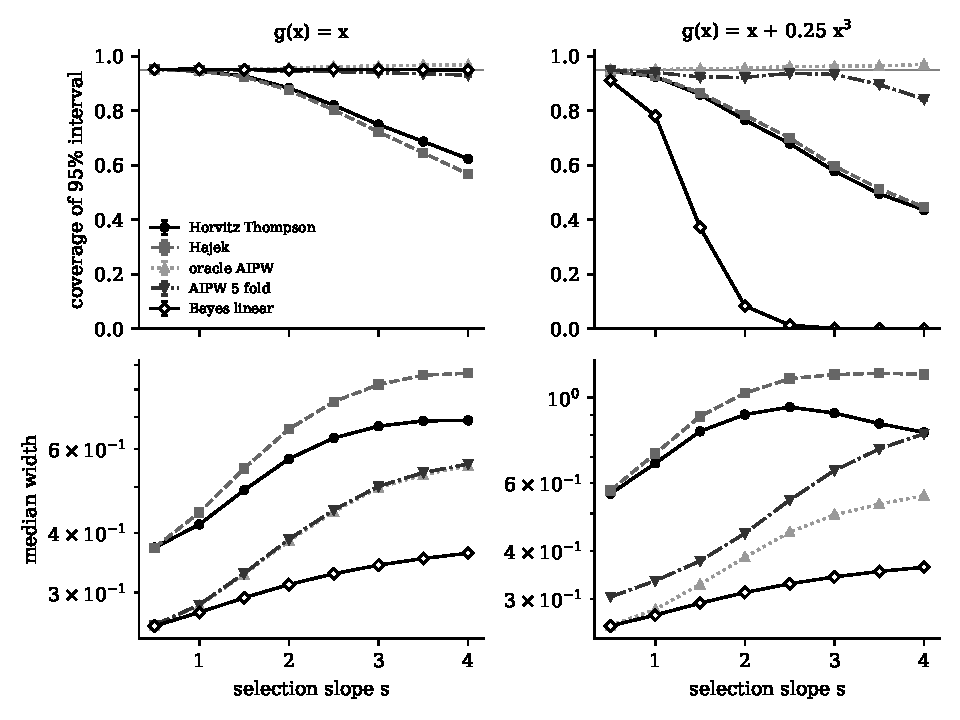
\includegraphics[width=\linewidth]{ipw_overlap_coverage.pdf}
\caption{Coverage of nominal 95 percent intervals (top) and median interval width (bottom) as overlap deteriorates, $n = 1000$, 20,000 replications per point; left $g(x) = x$, right $g(x) = x + 0.25x^3$. Binomial standard errors of the coverages are at most 0.0035.}
\label{fig:ipwcov}
\end{figure}

The augmented score of Chapter~\ref{ch:dml} still divides residuals by $e(X)$ and $1 - e(X)$. With true outcome regressions, its variance here is $2\{1 + \exp(s^2/2)\}/n$ (Exercise~\ref{ex:ch05:3}, applied to both arms), giving a standard deviation of 2.4 at $s = 4$ against 9.3 for \eqref{eq:ipw}. A good outcome model limits the damage by keeping residuals small; with a poor one, weighted residuals behave as badly as \eqref{eq:ipw}.

\section{Trimming changes the question}

The standard remedy for poor overlap\index{overlap!trimming|textbf} is trimming\index{trimming|textbf}: discard units with $e(x)$ outside $[\alpha, 1 - \alpha]$. Crump, Hotz, Imbens and Mitnik (2009) showed how to choose $\alpha$ to minimize variance. Li, Morgan and Zaslavsky (2018) proposed overlap weights\index{overlap weighting}, $1 - e(x)$ for treated units and $e(x)$ for controls, which downweight units near the extremes smoothly and target the population with covariate density proportional to $e(x)\{1 - e(x)\}$.

Both remedies are sensible and both change the estimand\index{estimand!changed by trimming|textbf}. The new estimands are accounting identities with particular choices of $Q$, chosen not because they answer the user's question but because they make an estimator behave.

A Bayesian faces the same lack of overlap. Where one arm is scarce, the posterior for $\tau(x)$ rests on the prior and on extrapolation. A prior that lets $\tau(x)$ vary gives wide intervals there, and for $\tau_Q$ when $Q$ puts mass there; hard pooling can give a narrow interval with no local data behind it. Report $\tau_Q$ for the user's $Q$ and check how its interval moves when the prior on $\tau(x)$ is loosened.

In the language of Chapter~\ref{ch:mccullagh}, let $\mathcal{X}_\alpha = \{x : \alpha \leq e(x) \leq 1 - \alpha\}$. The trimmed estimand\index{trimming!changes the estimand|textbf} is
\[
\tau_\alpha = \frac{\int_{\mathcal{X}_\alpha} \tau(x)\,Q(dx)}{Q(\mathcal{X}_\alpha)},
\]
which is $\tau_{Q_\alpha}$ for the restriction $Q_\alpha$ of $Q$ to $\mathcal{X}_\alpha$. The overlap\index{overlap} weighted estimand is $\tau_{Q_e}$ with $Q_e(dx) \propto e(x)\{1 - e(x)\}Q(dx)$.

\section{Double robustness and the Kang and Schafer example}

The augmented estimator is doubly robust\index{double robustness|textbf}\index{doubly robust|see{double robustness}}: consistent if either the outcome model or the propensity model is correct. Kang and Schafer (2007) tested this property in what became a standard benchmark\index{Kang and Schafer example|textbf}.

Their design has four latent covariates that determine both treatment and outcome, but the analyst observes only nonlinear transformations of them. Both models, fitted to the observed transformations, are therefore mildly misspecified. The augmented estimator then performed badly, sometimes worse than a simple regression estimator, because a few units with tiny estimated propensities received enormous weights that amplified small errors in the outcome model.

Kang and Schafer concluded that when both models are wrong, the usual case, double robustness guarantees nothing and the weighting component can make matters worse. In the discussion, Robins, Sued, Lei Gomez and Rotnitzky (2007) proposed bounded versions of the augmented estimator that perform better.

\section{Balancing weights}

Another response to unstable weights is to choose weights that balance covariates directly rather than invert an estimated propensity\index{balancing weights|textbf}. Hainmueller's (2012) entropy balancing\index{entropy balancing|textbf} chooses control weights as close as possible to uniform, in Kullback and Leibler divergence, subject to exact balance of chosen covariate moments with the treated group. Imai and Ratkovic's (2014) covariate balancing propensity score\index{propensity score} fits a propensity model whose implied weights balance covariates. Zubizarreta's (2015) stable balancing weights minimize weight variance subject to approximate balance.

If $\mu_0(x) = \phi(x)^\top\beta$ for a vector of features $\phi$, any control weights $w_i$ for which $\sum_i w_i\phi(X_i)$ equals the treated mean of $\phi$ give $\sum_i w_iY_i$ an expectation equal to the treated mean of $\mu_0$, whatever $\beta$ is, and the weighted difference in means is unbiased for the effect on the treated. Which features to balance is a modelling question about which functions of $x$ drive the outcome; the methods differ only in how they trade exact balance against dispersion of the weights.

Balancing weights therefore implicitly fit a linear outcome model in the balanced features, a step from Horvitz and Thompson\index{Horvitz Thompson estimator} to a full outcome model. A regression on the same features gets there directly: least squares with a full rank design implies control weights that balance the features exactly, some of them negative, while a Bayesian regression with a shrinkage prior gives up a little balance for less dispersed weights and reports a posterior as well. The practical difference is small when the features are few and well chosen. A balancing method with a long list of moments produces dispersed weights or fails to find any, while a shrinkage prior on the same list decides from the data which moments matter.

\section{Bayesian views of the propensity score}

Under ignorability and prior independence of outcome and treatment parameters, the propensity score\index{propensity score!Bayesian views of|textbf} drops out of the outcome posterior \eqref{eq:ignorable}, yet Bayesian analysts have used it for decades. Three uses are sound.

\paragraph{As a covariate.} Including the estimated propensity, or a flexible function of it, as a covariate in the outcome model protects against misspecification in the direction that matters for confounding. The device, used by the Bayesian causal forest and the coupled horseshoe of Chapter~\ref{ch:horseshoe}, is justified by the regularization induced confounding argument of Section~\ref{sec:rrw}.

\paragraph{As a dimension reduction.} Rosenbaum\index{Rosenbaum, Paul R.!propensity score} and Rubin's\index{Rubin, Donald B.!propensity score} 1983 theorem says that if treatment is ignorable given $X$ then it is ignorable given $e(X)$. Modelling the outcome as a function of $e(X)$ alone is a legitimate, though crude, outcome model.

\paragraph{As a prior input.} When the propensity is known, as in the Robins and Ritov example of Section~\ref{sec:rrw}, it is prior information about selection and belongs in the prior.

A fourth use needs care. A joint Bayesian model of propensity and outcome is coherent, but outcomes can feed back into the propensity estimate and pull it away from the assignment mechanism, breaking the design stage logic (Zigler and coauthors 2013). Fitting the propensity first and fixing it, or using a modular posterior, avoids this. The coupled horseshoe\index{horseshoe prior} of Chapter~\ref{ch:horseshoe} shares scales, but each model's coefficients use only its own data, limiting feedback to scale parameters.

\section{Matching and Bayesian imputation: a care management example}\label{ss:ipw:health}
\newcommand{\hcnmem}{20{,}000}
\newcommand{\hcntreat}{4{,}482}
\newcommand{\hcnmatch}{4{,}170}
\newcommand{\hcmeantreat}{16{,}822}
\newcommand{\hcmeancontrol}{9{,}655}
\newcommand{\hcnaive}{7{,}168}
\newcommand{\hcmatch}{-629}
\newcommand{\hcmatchse}{382}
\newcommand{\hcbayes}{-1{,}585}
\newcommand{\hcbayeslo}{-2{,}423}
\newcommand{\hcbayeshi}{-825}
\newcommand{\hctruth}{-2{,}145}
\newcommand{\hctruthm}{-1{,}906}
\newcommand{\hcnetbayes}{1{,}185}
\newcommand{\hcppays}{1.00}
\newcommand{\hcnetmatch}{229}
\newcommand{\hcnetbook}{0.95}
\newcommand{\hcsmdpriorB}{0.87}
\newcommand{\hcsmdpriorA}{0.05}
\newcommand{\hcsmdhbaB}{0.62}
\newcommand{\hcsmdhbaA}{0.04}
\newcommand{\hcsmdcomB}{0.52}
\newcommand{\hcsmdcomA}{0.04}
\newcommand{\hcsmdageB}{0.17}
\newcommand{\hcsmdageA}{0.03}


Insurer programs are almost never randomized, so health services researchers and actuaries rely on propensity score matching. In a diabetes care management program, nurses call members, review medications, schedule eye and foot exams and follow up after hospital discharge. The insurer pays per enrolled member and asks whether claims fall by more than the fee. Enrollment targets members who are expensive, poorly controlled or have several comorbidities, and high costs tend to persist. Comparing enrolled and nonenrolled members confounds the program with referral.

We illustrate with a synthetic claims file of \hcnmem\ members built to resemble such evaluations. Age is $N(58, 10^2)$, HbA1c is $N(7.8, 1.2^2)$, the number of comorbidities is Poisson with mean $1.5$, and log prior year cost is $N(8.6, 0.9^2)$ plus $0.15$ per comorbidity plus $0.10$ per point of HbA1c above $7.8$. Write $a$, $h$, $c$ and $l$ for age less 58 divided by 10, HbA1c less $7.8$, comorbidities less $1.5$ and log prior cost less $8.8$. Enrollment is logistic with logit $-1.6 + 0.2a + 0.5h + 0.35c + 0.9l$, which favours sicker and costlier members, and \hcntreat\ members enroll. Next year cost is $\exp(8.8 + 0.06a + 0.12h + 0.10c + 0.65l + 0.8\varepsilon)$ with $\varepsilon$ standard normal, so it is log normal and persistent in prior cost. The program multiplies each enrolled member's cost by $e^{-0.12}$, a cut of about 11\%. The fee is \$400 per enrolled member per year. One file is generated (seed 7) and every estimator below is applied to it, so the standard errors and intervals describe that file and not a repeated sampling experiment. All figures are synthetic and illustrative, not estimates for any real program.

\paragraph{The naive comparison.} Enrolled members cost \$\hcmeantreat\ next year against \$\hcmeancontrol\ for the rest, an apparent increase of \$\hcnaive\ per member. Read naively, the program costs money twice: the fee and the higher claims. Table~\ref{ss:ipw:tab:balance} shows why. Before matching, enrolled members are more than three quarters of a standard deviation more expensive in the prior year and more than half a standard deviation worse in HbA1c and comorbidity count.

\paragraph{Matching.} We fit a logistic regression for enrollment on the four covariates and match greedily on the estimated logit of the propensity score, without replacement and within a caliper of $0.2$ standard deviations of the estimated logit across all members: enrolled members are taken in decreasing order of the logit, and each is paired with the nearest unused nonenrolled member if one lies within the caliper. Of the \hcntreat\ enrolled members, \hcnmatch\ find a match. The rest sit at the top of the propensity range, where nonenrolled members are scarce: a handful have no nonenrolled member within the caliper at all, and the others find that the nearby ones were taken by earlier matches. Overlap in the sense of Section~\ref{sec:ignorability} holds, since a logistic propensity lies strictly between 0 and 1, but in a finite file it is thin at the top, and matching without replacement turns thin overlap into discarded members. After matching every standardized mean difference is at most $0.05$ in absolute value.

\begin{table}[ht]
\centering
\begin{tabular}{@{}lrr@{}}
\toprule
Covariate & Before matching & After matching\\
\midrule
Age & $\hcsmdageB$ & $\hcsmdageA$\\
HbA1c & $\hcsmdhbaB$ & $\hcsmdhbaA$\\
Comorbidities & $\hcsmdcomB$ & $\hcsmdcomA$\\
Log prior year cost & $\hcsmdpriorB$ & $\hcsmdpriorA$\\
\bottomrule
\end{tabular}
\caption{Standardized mean differences, enrolled minus nonenrolled, in the synthetic care management example (one file of \hcnmem\ members).}
\label{ss:ipw:tab:balance}
\end{table}

The matched estimate of the change in next year cost is \$\hcmatch\ per enrolled member, with standard error \$\hcmatchse. The sign has reversed. After the \$400 fee, estimated savings are about \$\hcnetmatch\ per matched member, roughly \$\hcnetbook\ million a year across the \hcnmatch\ matched members. This is less than one standard error, so matching cannot tell whether the program pays. The target covers matchable members, not all \hcntreat\ enrolled, so the estimate is not scaled to the whole program. In this synthetic population the true effect on the matched members is \$\hctruthm: matching misses about two thirds of the saving. Even standardized differences of at most $0.05$ leave matched nonenrolled members cheaper in expectation: exponential, skewed costs turn small covariate differences into a gap large next to the saving.

\paragraph{The Bayesian version.} Rubin's (1978) prescription is to model the outcome and impute the missing potential outcomes. Among nonenrolled members we fit $\log Y_i \mid x_i \sim N(d_i^\top\beta, \sigma^2)$ with $d_i = (1, a_i, h_i, c_i, l_i)^\top$, under the noninformative prior $\pi(\beta, \sigma^2) \propto 1/\sigma^2$. For each of 2,000 posterior draws we impute the untreated cost of every enrolled member from the posterior predictive distribution and average observed minus imputed cost, so the target is the average effect on the \hcntreat\ enrolled members of this file. Each imputation is drawn without reference to the member's observed treated cost, which is the working assumption that the two potential outcomes are conditionally independent given the covariates and the parameters. Section~\ref{sec:imputation} explains that this association is not identified by the data; the simulation in fact sets $Y_i(1) = e^{-0.12} Y_i(0)$, perfect dependence, so the width of the interval and the probability below rest on a choice the data cannot check. Under this prior the predictive distribution of log cost is Student $t$, so predictive cost, and with it the posterior mean of the effect, is not finite, although with more than 15,000 degrees of freedom no set of 2,000 draws would show it; we therefore report posterior medians and quantiles. The posterior median of the effect on the treated is \$\hcbayes\ with central 95\% interval (\$\hcbayeslo, \$\hcbayeshi), which covers the true value of \$\hctruth\ for all enrolled members. This estimand includes the high propensity members that matching discarded, and it is larger in magnitude because the program saves most where costs are highest. The posterior also answers the insurer's question: the probability that savings exceed the \$400 fee is above $0.99$, and the posterior median net saving is \$\hcnetbayes\ per enrolled member. No point estimate with a standard error provides that probability directly.

\paragraph{Lessons.} Prior year cost is the dominant confounder, and without it no adjustment is credible. A before and after comparison of the enrolled alone is no substitute: regression to the mean pulls high cost members down, any rise in costs across the whole file pushes them up, and the bias can go either way. In this file average cost is higher next year than in the prior year, that rise outweighs regression to the mean, and the comparison understates the saving. Claims are skewed, with a heavy right tail, so a mean based estimate is noisy; a model for the cost distribution, here log normal and in practice a two part model with a point mass at zero, uses the data more efficiently and delivers distributional effects, such as the change in the probability of a member exceeding a stop loss threshold, that matter for reinsurance. In high dimensional claims data, with thousands of diagnosis and procedure codes as candidate confounders, the outcome model needs the horseshoe prior of Chapter~\ref{ch:horseshoe}.

\section{The weighting estimator as a posterior mean}

The inverse weighted estimator is close to a posterior mean without being one. In a covariate cell $x$ with $n_x$ units and $n_{x1}$ treated, the inverse weighted estimate of the treated potential outcome mean $\mu_1(x)$ is the observed treated mean times $n_{x1}/\{n_xe(x)\}$. Under a flat prior and normal likelihood the observed mean is the posterior mean when $n_{x1} > 0$; when $n_{x1} = 0$, weighting returns zero and the flat prior gives no posterior at all. Since $n_{x1} \sim \mathrm{Binomial}\{n_x, e(x)\}$, a cell with $n_x = 20$ and $e(x) = 0.1$ expects two treated units, so the factor $n_{x1}/2$ equals one with probability 0.29, zero with probability 0.12, and two or more with probability 0.13. The factor has expectation one but adds noise without information, which is why weighting is typically worse in mean squared error than cellwise regression when cells are well populated.

When cells are sparse and many have no treated units, the regression estimator needs a model to fill the empty cells, while the weighted estimator averages over the units it has. This is the regime of Robins and Ritov\index{Robins and Ritov example} (Section~\ref{sec:rrw}), where the choice of prior becomes decisive.

\section{The Robins, Ritov and Wasserman challenge}\label{sec:rrw}

The strongest argument against Bayesian causal inference is an example. Robins and Ritov\index{Robins and Ritov example|textbf}\index{Robins Ritov Wasserman example|see{Robins and Ritov example}} introduced it in 1997; Wasserman popularized it. The example appears to show that any Bayesian procedure whose prior ignores the known propensity score\index{propensity score}\index{propensity score!known|textbf} must fail while Horvitz and Thompson succeed. There is no misspecification and no hidden confounder, only many cells, a known selection probability for each, and a Bayesian who declines to use it. The reply is short: the propensity score is prior information, and a prior that uses it need not fail.

\subsection{The example}

Let $X$ take values in $K \gg n$ cells; equivalently, take $X$ uniform on a high dimensional cube and assume nothing about smoothness. Each cell $x$ has a known selection probability\index{selection probability|textbf} $e(x) \in [\delta, 1 - \delta]$ and an unknown outcome probability $\vartheta(x) \in [0,1]$.

Each unit draws $X$ uniformly, is selected with $R \sim \mathrm{Bernoulli}\{e(X)\}$, and if selected reveals $Y \sim \mathrm{Bernoulli}\{\vartheta(X)\}$. The target is
\[
\psi = \E\,\vartheta(X) = \frac{1}{K}\sum_{x} \vartheta(x),
\]
the mean outcome in the population. In causal language, $R$ is treatment, $Y$ is the potential outcome under treatment, $e$ is the propensity score, and $\psi$ is the mean of $Y(1)$.

\paragraph{The Horvitz Thompson estimator.} Since $e$ is known,
\[
\hat\psi_{\mathrm{HT}} = \frac{1}{n}\sum_{i=1}^n \frac{R_i Y_i}{e(X_i)}
\]
is unbiased with variance at most $1/(n\delta)$. It converges at the $\sqrt{n}$ rate uniformly over all $\vartheta$, however rough.

\paragraph{The likelihood.} Up to a factor that involves $e$ and not $\vartheta$,
\[
L(\vartheta) \propto \prod_{i: R_i = 1} \vartheta(X_i)^{Y_i}\{1 - \vartheta(X_i)\}^{1 - Y_i}.
\]
So for any prior on $\vartheta$ independent of $e$, the posterior for $\vartheta$, and hence for $\psi$, does not depend on $e$ at all.

\subsection{The failure}

Since $K \gg n$, most cells are never visited, their posterior for $\vartheta(x)$ equals the prior, and the posterior for $\psi$ is dominated by the prior over unvisited cells\index{Robins and Ritov example!the failure|textbf}.

\begin{proposition}
Suppose $\vartheta(x)$ are a priori independent across cells, each with prior mean $\mu_0$, and independent of $e$. If $n/K \to 0$, then the posterior mean of $\psi$ converges in probability to $\mu_0$ whatever the true $\vartheta$.
\end{proposition}

\begin{proof}
Unvisited cells keep prior mean $\mu_0$; each of the at most $n$ visited posterior means differs from $\mu_0$ by at most one. Thus $|\E(\psi \mid \text{data}) - \mu_0| \leq n/K \to 0$.
\end{proof}

The Bayesian estimate is inconsistent, while Horvitz and Thompson\index{Horvitz Thompson estimator} converge at the parametric rate.

A hierarchical prior, with the cell probabilities exchangeable around an unknown mean, would learn $\mu_0$ from the data, but it would learn the mean among selected units, which is $\E\{e(X)\vartheta(X)\}/\E\,e(X)$, not $\psi$. When $\vartheta$ and $e$ are correlated, the two differ and the hierarchical posterior converges to the wrong answer: the selected units are not representative, and a prior that ignores selection cannot know it.

\subsection{A simulation of the failure}

We set $K = 20{,}000$ cells and $n = 2{,}000$ units\index{Robins and Ritov example!a simulation of the failure|textbf}\index{simulation study!Robins and Ritov failure|textbf}. Selection probabilities are uniform on $[0.05, 0.95]$. Outcome probabilities depend on selection: $\logit\vartheta(x) = -1 + 6\{e(x) - 0.5\} + \eta(x)$, with $\eta(x) \sim N(0, 0.3^2)$. Units likely to be selected have high outcome probability, so the selected units overstate $\psi$.

We compare three estimators over 200 replications: Horvitz Thompson; the posterior mean under independent uniform priors on each $\vartheta(x)$; and an empirical Bayes\index{empirical Bayes} version of the coupled prior \eqref{eq:coupled} introduced below. For the last, a logistic regression of the selected outcomes on $\logit e$ gives a fitted probability $m_x = \expit\{\hat a + \hat b\,\logit e(x)\}$ for every cell, each $\vartheta(x)$ gets a $\mathrm{Beta}\{10m_x, 10(1 - m_x)\}$ prior, worth ten observations, and the estimate is the average over all $K$ cells of the posterior means $(10m_x + S_x)/(10 + N_x)$, where $N_x$ and $S_x$ count the selected units and successes in cell $x$. The beta prior stands in for the logistic normal of \eqref{eq:coupled}, $\sigma_\eta$ is not estimated, and the uncertainty in $\hat a$ and $\hat b$ is ignored.

\begin{figure}[ht]
\centering
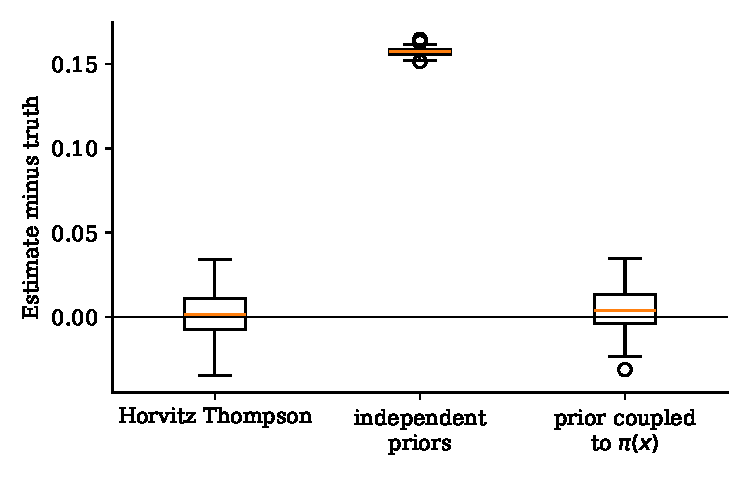
\includegraphics[width=\linewidth]{robins_ritov.pdf}
\caption{Error of three estimators in the Robins and Ritov example, 200 replications, $K = 20{,}000$ and $n = 2{,}000$.}
\label{fig:rr}
\end{figure}

\begin{table}[ht]
\centering
\caption{Bias and root mean squared error in the Robins and Ritov example.}
\label{tab:rr}
\begin{tabular}{lcc}
\toprule
Estimator & Bias & RMSE \\
\midrule
Horvitz Thompson & 0.002 & 0.014 \\
Independent priors & 0.157 & 0.157 \\
Prior coupled to $e(x)$ & 0.005 & 0.013 \\
\bottomrule
\end{tabular}
\end{table}

In Figure~\ref{fig:rr} and Table~\ref{tab:rr}, the independent prior posterior is off by 0.157 with almost no spread: confidently wrong, as the proposition predicts. The coupled prior matches Horvitz and Thompson.

\subsection{The resolution}

Sims's response to Wasserman was that a Bayesian who knows $e$, and believes $\vartheta$ may be related to it, should say so in the prior\index{Robins and Ritov example!the resolution|textbf}. The prior independence of $\vartheta$ and $e$ is not a requirement of Bayesian inference; it is a modelling choice, and in this example a bad one.

Formally, replace the independent prior by a prior in which $\vartheta(x)$ depends on $e(x)$\index{coupled prior!for the selection probability|textbf}:
\begin{equation}
\logit\vartheta(x) = a + b\,\logit e(x) + \eta(x), \qquad \eta(x) \sim N(0, \sigma_\eta^2).
\label{eq:coupled}
\end{equation}
Now cells are partially exchangeable given $e$: two cells with the same selection probability are judged alike, others are not. Write $\xi = (a, b, \sigma_\eta)$ and $q_\xi(p) = \E\,\expit\{a + b\,\logit p + \sigma_\eta Z\}$ with $Z \sim N(0, 1)$. Given $e(X) = p$, a selected unit's outcome is Bernoulli with probability $q_\xi(p)$, so $\xi$ is learned from the selected units, across which $e$ varies. What matters for $\psi$ is the fitted curve $q_\xi$: given $\xi$, the posterior for an unvisited cell has median $\expit\{a + b\,\logit e(x)\}$ and mean $q_\xi\{e(x)\}$, which is the right place, and its posterior mean is $q_\xi\{e(x)\}$ averaged over the hyperposterior of $\xi$.

\begin{theorem}
Suppose the true $\vartheta$ is drawn from \eqref{eq:coupled} at an interior $\xi_0$, the hyperprior on $\xi$ has a continuous positive density at $\xi_0$, the empirical distribution of $e$ over the cells converges, and the marginal model of the selected outcomes, Bernoulli with probability $q_\xi\{e(X)\}$, meets the conditions of the parametric Bernstein von Mises theorem of Appendix~\ref{app:theory}, nonsingular Fisher information included. If $K/n^{3/2} \to \infty$, the posterior for $\psi$ concentrates at the truth at the $\sqrt{n}$ rate.
\end{theorem}

\begin{proof}[Sketch]
The number of selected units is binomial with mean at least $n\delta$. The expected number of pairs of draws that land in the same cell is $n(n - 1)/(2K) = o(\sqrt{n})$, since $K/n^{3/2} \to \infty$. Each such pair changes the log likelihood ratio between $\xi_0$ and a point within $O(n^{-1/2})$ of it by $O(n^{-1/2})$. Repeated cells therefore change that ratio by $o_p(1)$, so the stated conditions give a posterior for $\xi$ that concentrates at $\xi_0$ at the $\sqrt{n}$ rate. Given $\xi$, the average over the cells is $K^{-1}\sum_x q_\xi\{e(x)\}$ up to $O_p(K^{-1/2})$, a smooth function of $\xi$ whose posterior inherits the rate by the delta method. Visited cells change the average by $O(n/K)$. Both remainders are $o(n^{-1/2})$ because $K/n^{3/2} \to \infty$. The simulation of this section, with $K = 20{,}000$ and $n = 2{,}000$, lies outside this regime ($n/K = 0.1$ against $n^{-1/2} = 0.022$), so the theorem does not cover it.
\end{proof}

If \eqref{eq:coupled} is misspecified and the hyperposterior concentrates at a finite $\xi^\ast$, that point best fits the selected units, minimizing
\[
\E[e(X)\,\KL\{\mathrm{Bernoulli}(\vartheta(X)) \,\|\, \mathrm{Bernoulli}(q_\xi\{e(X)\})\}].
\]
Concentration at a finite point can fail: $\vartheta \equiv 0$ pushes $a$ to $-\infty$. When $n/K \to 0$, the posterior mean of $\psi$ is off by $K^{-1}\sum_x [q_{\xi^\ast}\{e(x)\} - \vartheta(x)]$, the curve's misfit averaged over all cells, not over the selected ones. The remedy is a more flexible regression: a spline, or a horseshoe\index{horseshoe prior} expansion in basis functions of $e$. With enough flexibility and enough selected units in every stratum of $e$ for the prior to wash out, the posterior mean approaches H\'ajek stratified by $e$ (Ritov, Bickel, Gamst and Kleijn 2014).

\subsection{The Sims and Wasserman exchange}

Around 2012 the example was argued over on Wasserman's blog\index{Sims and Wasserman exchange|textbf}. Robins and Wasserman held, in substance, that a prior depending on $e$ is a frequentist device in Bayesian clothing, since $e$ does not appear in the likelihood for $\vartheta$. Sims (2012) answered that $e$ is known before the data, and anything known before the data may enter the prior. The likelihood principle\index{likelihood principle} constrains how data enter inference, not which prior information may be used.

We side with Sims; the coupled prior is a parametric version of his proposal. If the analyst genuinely believes that $\vartheta$ and $e$ are unrelated, an exchangeable hierarchical prior that ignores $e$ is correct, the selected units are representative, and that posterior is consistent; independent cell priors with a fixed centre are not, as the proposition above shows. The failure arises when the prior contradicts what the analyst actually believes.

\subsection{A Bayesian derivation of binned H\'ajek}

Partition the range of $e$ into bins\index{Hajek estimator@H\'ajek estimator!binned} and give each bin its own exchangeable prior on $\vartheta$, a fully flexible version of the coupled prior. As the bins shrink, slowly enough that each keeps many selected units, the selected units in a bin are a simple random sample of its cells. In the simplest version every cell of bin $j$ shares one outcome probability with a $\mathrm{Beta}(\alpha_j, \beta_j)$ prior, and if the bin holds a share $W_j$ of the cells, $M_j$ selected units and $S_j$ successes, the posterior mean of $\psi$ is $\sum_j W_j(\alpha_j + S_j)/(\alpha_j + \beta_j + M_j)$; with $\alpha_j = \beta_j = 1$ this is the bin posterior of Section~\ref{sec:weak}. As the $M_j$ grow it approaches $\sum_j W_jS_j/M_j$; a bin with no selected unit keeps its prior mean.

Estimating the shares from the sample and dropping empty bins turns this into the binned H\'ajek estimator, H\'ajek weighting stratified by propensity. Horvitz and Thompson differ from it in normalization and in the absence of binning, and have a different first order variance. So binned H\'ajek is, to this approximation, the limit of posterior means under a nonparametric prior in which $\vartheta$ is exchangeable given $e$: not a rival to Bayes but a special case, with a very weak prior on how outcomes depend on selection.

\subsection{CODA and the curse of dimensionality}

Classical asymptotics fix the model as the sample grows. Robins and Ritov let the complexity of $\vartheta$ grow too, calling this curse of dimensionality appropriate, or CODA, theory\index{curse of dimensionality appropriate asymptotics|textbf}\index{CODA|see{curse of dimensionality appropriate asymptotics}}.

The CODA question is whether an estimator converges uniformly over a class of $\vartheta$ so large that no estimator of $\vartheta$ itself converges: whether, for a class $\Theta$,
\[
\sup_{\vartheta \in \Theta} \E_\vartheta(\hat\psi - \psi)^2 \to 0
\]
at a stated rate as $n \to \infty$. Horvitz and Thompson do, for $\psi$, because the bound $1/(n\delta)$ on their variance does not depend on $\vartheta$. Bayesian estimators with priors that do not use $e$ do not. Ritov, Bickel, Gamst and Kleijn's 2014 paper examines which Bayesian procedures are CODA, and finds that those using $e$ in the prior, or using the propensity score\index{propensity score} as a covariate, can be.



\subsection{What the example does and does not show}

The example shows that a prior ignoring known selection probabilities can fail badly in high dimensions\index{Robins and Ritov example!what it does and does not show|textbf}. It does not show that Bayesian inference fails, only that a particular prior does.

The Horvitz Thompson estimator is good only for $\psi$. Ask for a quantile of $\vartheta(X)$, $\vartheta$ in a subgroup, or the effect on a new population with different covariate law, and a new weighted estimator must be built. The coupled posterior delivers all of them.

When $\vartheta$ is smooth in $x$, a smooth prior learns about unvisited cells from visited neighbours, so prior independence of $\vartheta$ and $e$ does little harm. The example bites only when $\vartheta$ is so rough that $x$ carries no information across cells, but $e$ does. That is when the analyst should model $\vartheta$ as a function of $e$.

\paragraph{When the propensity is estimated.}
In observational studies $e$ must be estimated from the same high dimensional data, and may be as rough as $\vartheta$. Yet treatment is observed for every unit, while each outcome model sees only one arm. The propensity can therefore often be estimated well even when the outcome surface cannot, and using it in the outcome prior transfers that information. This asymmetry supports the propensity covariate device and the Bayesian causal forest\index{Bayesian causal forest}'s use of $\hat e(X)$ as a covariate.

\subsection{Regularization induced confounding}

The same mechanism appears in the partially linear model of Chapter~\ref{ch:dml} as regularization induced confounding\index{regularization induced confounding|textbf} (Hahn, Carvalho, Puelz and He 2018). A shrinkage prior on the confounder coefficients, independent of the treatment model, shrinks a true confounder toward zero. Its outcome variation is attributed to the correlated treatment, biasing $\tau$ in the direction of the confounding.

The remedy is the same: an unpenalized propensity covariate $\hat m(X)$, this chapter's $\hat e(X)$, lets the outcome prior depend on the treatment model and protects the confounding direction from shrinkage. In Section~\ref{sec:ricsim} of Chapter~\ref{ch:horseshoe}, coupling to the whole sample propensity reduced independent horseshoe bias from 0.059 to $-0.023$; DML bias was 0.009 (Table~\ref{tab:ric}). At $p = 50$, least squares on all the covariates matched the coupled posterior (root mean squared error 0.084 for both, least squares bias $-0.002$). At $p = 150$ and 300, DML stayed more accurate while coupled bias grew to $-0.045$ and $-0.071$. With thirty weak confounders at $p = 150$, the order reversed: coupled bias 0.004 against DML's 0.069.

\section{Horvitz Thompson, H\'ajek and the weak paradoxes}\label{sec:weak}

This section develops the work of Datta and Polson (2026) on inverse probability weighting\index{inverse probability weighting}. We set the Horvitz Thompson\index{Horvitz Thompson estimator} and H\'ajek\index{Hajek estimator@H\'ajek estimator} estimators side by side, criticize H\'ajek as a halfway house to a model that does not go far enough, and reply to the claim of Ritov, Bickel, Gamst and Kleijn about the hierarchical Bayes estimator in the Robins, Ritov and Wasserman problem\index{weak paradoxes|textbf}, a claim that is true as stated and misleading in what it leaves out.

\subsection{Two estimators}

In survey notation the estimators of Section~\ref{sec:hajek} read as follows. Let units $k = 1, \ldots, n$ have fixed bounded outcomes $Y_k$, observed when $R_k = 1$, with independent $R_k \sim \mathrm{Bernoulli}(p_k)$ and $p_k \geq \delta > 0$ known. Write
\[
\hat S = \sum_{k=1}^n \frac{R_k Y_k}{p_k}, \qquad \hat n = \sum_{k=1}^n \frac{R_k}{p_k}.
\]
The Horvitz Thompson and H\'ajek estimators of the mean $\psi$ are
\[
\hat\psi_{\mathrm{HT}} = \frac{\hat S}{n}, \qquad \hat\psi_{\mathrm{H}} = \frac{\hat S}{\hat n}.
\]
Horvitz and Thompson are exactly unbiased over the design. H\'ajek is a ratio, nonlinear and biased at order $1/n$, and it does not need $n$, which is why it is the only option when the population size is unknown. Trotter and Tukey\index{Horvitz Thompson estimator!Trotter and Tukey interpolation|textbf} in 1956 interpolated between them,
\[
\hat\psi_{\lambda} = \frac{\hat S}{(1 - \lambda)n + \lambda\hat n},
\]
and Khan and Ugander studied this family in 2023 as adaptive normalization\index{adaptive normalization|textbf}, choosing $\lambda$ from the data so that the asymptotic variance is never above that of either endpoint.

In this family $\lambda = 0$ trusts the design, $\lambda = 1$ trusts the realized sample, and an intermediate $\lambda$ hedges. Adaptive normalization chooses the hedge to minimize an estimated variance, which is already a step toward modelling, since that variance depends on the outcomes.

\subsection{When H\'ajek wins, and why}

S\"arndal, Swensson and Wretman (2003) identify three situations in which H\'ajek tends to have lower variance than Horvitz and Thompson\index{Hajek estimator@H\'ajek estimator!when it wins}: when the outcomes are close to their mean, the extreme case being a constant outcome; when the sample size is random with equal inclusion probabilities; and when inclusion probabilities are negatively correlated with outcomes, so that large outcomes carry large weights. Basu\index{Basu elephants@Basu's elephants}'s circus is the first: whichever elephant is drawn, H\'ajek estimates the total as fifty times its weight.



\begin{proposition}
To first order,
\[
\hat\psi_{\mathrm{H}} - \psi \approx \frac{1}{n}\sum_{k=1}^n \frac{R_k(Y_k - \psi)}{p_k},
\qquad
\hat\psi_{\mathrm{HT}} - \psi = \frac{1}{n}\sum_{k=1}^n \left(\frac{R_kY_k}{p_k} - \psi\right).
\]
H\'ajek is Horvitz and Thompson applied to the centred outcomes $Y_k - \psi$.
\end{proposition}

\begin{proof}
Write $\hat\psi_{\mathrm{H}} - \psi = (\hat S - \psi\hat n)/\hat n$ and replace $\hat n$ by its expectation $n$ in the denominator.
\end{proof}

Centring removes the variance due to the level of the outcome. If every outcome equals $c$, Horvitz and Thompson still vary because $\hat n$ varies, while H\'ajek is exact. In survey language, H\'ajek is the model assisted estimator whose working model is a common mean. Under the independent Bernoulli design the first order variances of Horvitz and Thompson and of H\'ajek differ by $n^{-2}\psi\sum_k (1 - p_k)(2Y_k - \psi)/p_k$, so H\'ajek wins exactly when this difference is positive. Large outcomes on units with small $p_k$ push it up, which is the third situation, but a negative correlation between $p_k$ and $Y_k$ does not guarantee it: with equal numbers of units of the types $(p_k, Y_k) = (0.01, 0)$, $(0.1, 1)$ and $(0.99, 0)$ the correlation is negative, yet H\'ajek's first order variance is $5.0/n$ against $3/n$ for Horvitz and Thompson.

\subsection{A critique of the H\'ajek estimator}

The proposition also shows what H\'ajek does not do\index{Hajek estimator@H\'ajek estimator!critique of}. In the setting of the Robins, Ritov and Wasserman example, with cells $b = 1, \ldots, B$, outcome probabilities $\theta_b$ and selection probabilities $p_b$ (Section~\ref{sec:rrw} writes $K$, $x$, $e(x)$ and $\vartheta(x)$ for $B$, $b$, $p_b$ and $\theta_b$), its asymptotic variance is
\[
\mathrm{Var}(\hat\psi_{\mathrm{H}}) \approx \frac{1}{n}\cdot\frac{1}{B}\sum_{b=1}^B \frac{\theta_b(1 - \theta_b) + (\theta_b - \psi)^2}{p_b},
\]
while for Horvitz and Thompson the numerator is $\theta_b$ and a $-\psi^2$ term is subtracted outside the sum. Both variances carry the factor $1/p_b$: H\'ajek lowers the numerator in cells with $\theta_b > \psi/2$, raises it in cells with $\theta_b < \psi/2$, and does nothing about the denominator. As some selection probabilities approach zero, both estimators degrade. In the first design of Table~\ref{tab:weak} the outcome probabilities are uniform on $[0.1, 0.9]$ and independent of selection, and the mean of $1/p_b$ over $[0.01, 0.99]$ is about 4.7. The two formulas then give about 2.1 for Horvitz and Thompson and 1.2 for H\'ajek on the scale of the table (mean squared error times 100), against the simulated 2.08 and 0.96.

We draw four criticisms from this. First, H\'ajek is a model that will not admit it is one: its gain over Horvitz and Thompson comes entirely from an implicit common mean. Its fix for Basu's circus, ratio estimation with an auxiliary size variable $A_k$, is a regression model through the origin. Once a model does the work, the analyst should state it and choose it well.

Second, H\'ajek keeps the weights. Every observed outcome is still multiplied by $1/p_k$, and a tiny $p_k$ lets one unit dominate numerator and denominator together. The ratio partly cancels the damage but cannot remove it.

Third, H\'ajek cannot borrow strength: two cells with similar selection probabilities and outcome rates share only a normalizer. This is where Stein's paradox\index{Stein paradox@Stein's paradox|textbf} enters: for Gaussian observations with known variance, in three or more dimensions the James Stein estimator\index{James Stein estimator|textbf}, which pools, dominates the cellwise estimator of the vector of means under summed squared error (James and Stein 1961). The cells here are Bernoulli and the target is one average, so the theorem does not transfer as it stands, but it is the reason to expect pooling to help, and neither Horvitz and Thompson nor H\'ajek pools.

Fourth, H\'ajek gives no distribution: a point estimate and a linearized variance, but no posterior for $\psi$, no answer for any other functional, and no indication of which cells drive the uncertainty.

\subsection{The weak paradoxes}

Datta and Polson study what J.~K. Ghosh\index{Ghosh, Jayanta K.!weak paradoxes|textbf} called weak paradoxes\index{weak paradoxes}: Basu's circus and the Robins, Ritov and Wasserman example of Section~\ref{sec:rrw}. Several Bayesian responses have been proposed.

Li, in 2010, made the cell probabilities exchangeable around a hypermean $h$, $\theta_b \sim \mathrm{Beta}(\alpha_T h, \alpha_T(1 - h))$, with a $\mathrm{Beta}(\alpha_F, \alpha_F)$ prior on $h$. With $\alpha_F = 1$ and no cell observed twice, the posterior mean of $h$ is
\[
\hat\psi_{\mathrm{Li}} = \frac{\sum_k R_kY_k + 1}{\sum_k R_k + 2}.
\]
This is the estimator we study. The finite population mean $\psi = B^{-1}\sum_b \theta_b$ is not $h$: with $M = \sum_k R_k$ selected units and $S = \sum_k R_kY_k$ successes, its posterior mean is $\hat\psi_{\mathrm{Li}} + (S - M\hat\psi_{\mathrm{Li}})/\{B(\alpha_T + 1)\}$, and the correction vanishes when the selected units are a small fraction of the cells.

Ghosh (2015) grouped the selection probabilities into $J \ll B$ bins and applied the weighting within bins, with each bin's mean selection probability in place of the individual $p_k$. Sims (2012) proposed treating $\theta$ as a step function of $p$, constant within segments of the range of $p$, a Bayesian version of the same binning. Harmeling and Toussaint (2007) replaced the Bernoulli outcome by a Gaussian with a hierarchical prior and showed that the posterior mean beats Horvitz and Thompson in mean squared error.

\subsection{Li's estimator revisited}

Ritov, Bickel, Gamst and Kleijn asserted that Li's estimator\index{Li estimator@Li's estimator|textbf} is consistent only if $\E(Y \mid R = 1) = \E(Y)$, that is, only if selection is unrelated to the outcome. Datta and Polson gave a proof and a sharper statement. Write
\[
\bar p = \frac{1}{B}\sum_b p_b, \qquad \sigma_{\theta,p} = \frac{1}{B}\sum_b \theta_b p_b - \bar p\,\psi.
\]

\begin{theorem}[Datta and Polson]
As $n \to \infty$,
\[
\E(\hat\psi_{\mathrm{Li}}) \to \psi + \frac{\sigma_{\theta,p}}{\bar p},
\]
and the variance of $\hat\psi_{\mathrm{Li}}$ is of order $1/n$ with a constant that involves only $\bar p$ and $B^{-1}\sum_b\theta_bp_b$, not the individual $1/p_b$.
\end{theorem}

\begin{proof}[Sketch]
The draws are independent, so $M = \sum_k R_k$ is binomial with $n$ trials and success probability $\bar p$, and given $M$ the number of successes $S = \sum_k R_kY_k$ is binomial with $M$ trials and success probability $q = B^{-1}\sum_b\theta_bp_b/\bar p = \psi + \sigma_{\theta,p}/\bar p$. Hence $\E(\hat\psi_{\mathrm{Li}} \mid M) = (Mq + 1)/(M + 2) = q + (1 - 2q)/(M + 2)$, and since $M/n \to \bar p > 0$ and the second term is bounded, $\E(\hat\psi_{\mathrm{Li}}) \to q$. The variances of numerator and denominator and their covariance are linear in $n$ with constants built from $\bar p$ and $B^{-1}\sum_b\theta_bp_b$; the delta method for a ratio gives the stated order.
\end{proof}

The theorem confirms Ritov and coauthors' claim: bias vanishes exactly when $\sigma_{\theta,p} = 0$. But Li's estimator needs no lower bound $p_b \geq \delta$: its variance contains no $1/p_b$. Its failure is the covariance between selection and outcome. Modelling that relation with the coupled prior of Section~\ref{sec:rrw} keeps the immunity to small $p_b$: rare cells are filled by extending the fitted relation instead of dividing rare observations by $p_b$. In the simulation below, coupling reduces bias from $0.050$ to $-0.001$ when selection is related to outcome; when unrelated, its error is about one and a half times Li's.

Ghosh's binning made Bayesian is a different case. With many selected units in every bin, its posterior mean is close to binned H\'ajek. In the simulation below binned H\'ajek has about H\'ajek's error, about twice Li's, when selection is unrelated to outcome. With ten bins and $n = 100$ draws that limit is far off: the prior pulls each bin toward one half, and the bin posterior of the simulation behaves quite differently.

Linero (2024) argues that in high dimensional and nonparametric models, Bayesian ignorability\index{ignorability} encodes an informative prior that selection bias is small.

\subsection{A simulation of six estimators}

We repeated and extended the simulation\index{simulation study!six estimators|textbf} of Datta and Polson. There are $B = 1{,}000$ cells with selection probabilities equally spaced on $[0.01, 0.99]$ and $n = 100$ draws of a cell chosen uniformly, so most cells are never seen. Outcome probabilities are uniform on one of four ranges and independent of selection. A fifth design makes selection informative, with $\theta_b = 0.5p_b + 0.5U_b$, $U_b$ uniform on $[0,1]$, and selection probabilities on $[0.1, 0.9]$. We compare Horvitz and Thompson, H\'ajek, Li's estimator, binned H\'ajek with ten bins, and the coupled prior, which centres each cell's outcome probability on a logistic regression on $\logit p_b$ fitted to the observed cells, each cell then having a beta prior with that mean and a weight of five observations. The sixth, a bin posterior, puts independent uniform priors on the mean outcome probability in ten bins of the selection probability and weights the bin means by the known shares of cells in the bins. Each design is replicated 5,000 times.

\begin{table}[ht]
\centering
\caption{Mean squared error times 100 in the weak paradox simulation. In the first four rows selection is independent of outcome; in the last row selection is related to the outcome. 5,000 replications; Monte Carlo standard errors are at most 0.11 for Horvitz and Thompson (HT) and 0.02 for the others except the bin posterior (0.004 to 0.013), and the paired standard errors of the differences between the coupled prior and the other estimators are 0.007 to 0.016 (HT excepted).}
\label{tab:weak}
\small
\begin{tabular}{lcccccc}
\toprule
Design & HT & H\'ajek & Li & Binned & Coupled & Bin post. \\
\midrule
$\theta \sim U[0.1, 0.9]$ & 2.08 & 0.96 & 0.47 & 0.92 & 0.71 & 0.22 \\
$\theta \sim U[0.1, 0.4]$ & 1.19 & 0.75 & 0.37 & 0.70 & 0.56 & 1.13 \\
$\theta \sim U[0.35, 0.65]$ & 2.18 & 0.98 & 0.46 & 0.92 & 0.70 & 0.22 \\
$\theta \sim U[0.6, 0.9]$ & 2.91 & 0.71 & 0.36 & 0.69 & 0.54 & 1.15 \\
Outcome related & 0.92 & 0.67 & 0.70 & 0.66 & 0.60 & 0.25 \\
\bottomrule
\end{tabular}
\end{table}

\begin{figure}[ht]
\centering
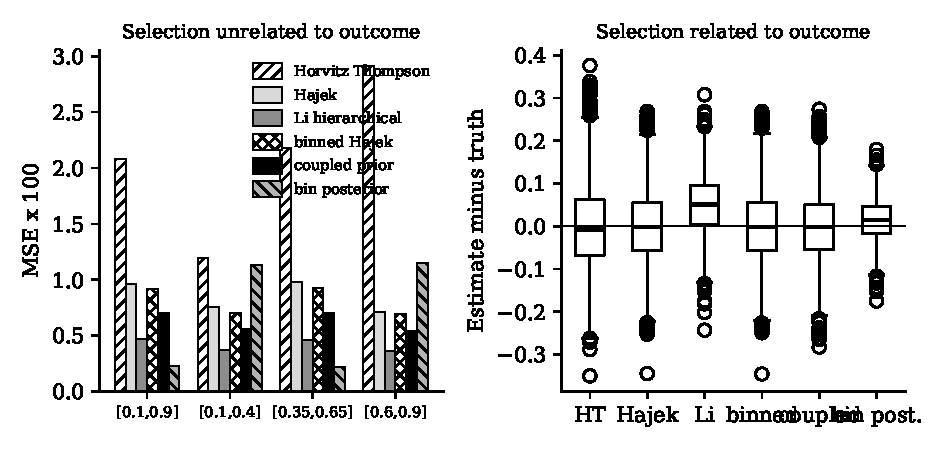
\includegraphics[width=\linewidth]{ipw_weak.pdf}
\caption{Left: mean squared error of six estimators (5,000 replications) when selection is unrelated to the outcome. Right: errors when selection is related to the outcome, where Li's estimator is biased upward.}
\label{fig:weak}
\end{figure}

Table~\ref{tab:weak} and Figure~\ref{fig:weak} reproduce the qualitative findings of Datta and Polson. When selection is unrelated to outcome, Li's hierarchical estimator has the smallest error of the five older estimators in every design, three to eight times smaller than Horvitz and Thompson, with H\'ajek and binned H\'ajek in between. When selection is related to outcome, Li's estimator is biased upward by 0.050, close to the 0.053 the theorem predicts, and its error is no better than H\'ajek's. The coupled prior is ahead of binned H\'ajek and H\'ajek in that design (0.60, 0.66 and 0.67; the gaps are 8.6 and 9.6 paired standard errors of 0.007) and is second best of the five when selection is unrelated to outcome, paying about one and a half times Li's error for estimating a regression on $\logit p$ that turns out flat. Its lead over H\'ajek and binned H\'ajek is more than ten paired standard errors in each of the four designs with selection unrelated to outcome.

The bin posterior is best near one half or under informative selection (0.22 to 0.25, against 0.46 to 0.70 for Li and 0.60 to 0.71 for the coupled prior), but worst among the model based estimators far from 0.5 ($U[0.1, 0.4]$ and $U[0.6, 0.9]$: 1.13 and 1.15, against 0.56 and 0.54 for the coupled prior, and worse than H\'ajek). Its uniform prior adds two observations at one half to every bin, so a bin with $M_j$ selected units and $S_j$ successes is estimated by $(1 + S_j)/(2 + M_j)$. With $n = 100$ draws a bin averages five selected units; the pull toward 0.5 gives biases of $+0.097$ and $-0.099$ in those two designs. About 9 percent of bins are empty and keep the prior mean, accounting for only about 0.022 of that bias. The prior pays off only when centred near the truth.

\subsection{Inverse weighting as importance sampling}

Datta and Polson's second theme is that the same estimators appear in Monte Carlo integration. Estimating $\psi = \int l(x)\,dF(x)$, the mean of a function $l$ under $F$, by sampling from a proposal $g$ and weighting by $f/g$ is Horvitz and Thompson with inclusion probabilities replaced by proposal densities. Self normalized importance sampling\index{importance sampling|textbf}, in which the weights are divided by their sum, is H\'ajek. The improvements known in Monte Carlo transfer back: Riemann sum and trapezoidal estimators that order the draws before summing (Yakowitz and coauthors, 1978; Philippe and Robert, 2001); vertical likelihood integration (Polson and Scott, 2014); nested sampling (Skilling, 2006); and quantile importance sampling (Datta and Polson, 2023), which orders draws by likelihood and can converge much faster for marginal likelihoods. Each replaces the raw weights by a smoother, ordered representation: binning and smoothing by another name.

The causal reading is direct: inverse propensity weighting\index{inverse probability weighting!as importance sampling|textbf} for the average treatment effect is importance sampling from the treated distribution to the population, and its instability when propensities are small is the familiar instability of importance sampling with a poor proposal. The Monte Carlo answer has always been to use the structure of the integrand; the causal analogue is an outcome model.

\subsection{From weak paradoxes to the horseshoe}

Datta and Polson propose a horseshoe\index{horseshoe prior} on cell deviations from a regression on selection probability. The global scale learns how much cells vary beyond what selection explains; local scales let a few differ sharply without pulling the others. This applies the prior of Chapter~\ref{ch:horseshoe} to missing data: model the relation between selection and outcome and borrow strength across cells.

\section{What the lineage teaches}

Three lessons run from Horvitz and Thompson to DML\index{double machine learning!lineage of weighting|textbf}\index{inverse probability weighting!lineage of|textbf}.

Design based unbiasedness is weak: it holds over hypothetical repeated assignments and says little about the actual one. Basu's elephants make this vivid; a treated unit in the far tail makes it practical. The estimator of Figure~\ref{fig:ipw} is unbiased at every selection slope, and at $s = 4$ even 300 replications could not pin down its standard deviation.

Every improvement adds modelling: a common mean (H\'ajek), a linear model (regression), a full outcome model (augmentation), keeping weights only as a correction. DML is the latest step, and it still depends on the weights through its correction term.

Robins and Ritov\index{Robins and Ritov example}'s example (Section~\ref{sec:rrw}) shows that ignoring the informative propensity score\index{propensity score} can be fatal. Model with it; do not weight by it. The coupled prior puts the selection probability where a Bayesian puts prior information, and in the simulation of that section it matched Horvitz and Thompson in error while delivering the posterior that Horvitz and Thompson cannot. The weights were a substitute for a model of the outcomes, and once the model is good enough they are no longer needed.

\section{In practice}

\paragraph{The target.} The target here is $\tau$, or its trimmed or overlap weighted versions, each $\tau_Q = \int \tau(x)\,Q(dx)$ for a different $Q$. All three come from one posterior for the outcome model, each draw $\tau^{(s)}$ giving the draw $\int \tau^{(s)}(x)\,Q(dx)$, and the user chooses $Q$ for substantive reasons. In the cell model, draw $(a, b, \sigma_\eta)^{(s)}$ and, for unvisited cells, $\vartheta(x)$ from \eqref{eq:coupled}; visited cells are updated by their data. Averaging gives $\psi^{(s)}$ for $\psi = K^{-1}\sum_x \vartheta(x)$. Subgroup means, new covariate laws and quantiles use the same draws.

\paragraph{What the analyst does differently.} An analyst who weights should first look at the weights. Report the largest weight and the effective sample size of the weights; a largest weight in the hundreds says that one or two units decide the estimate, as Jumbo would have decided the circus total. Normalize, though H\'ajek leaves a bias of order $1/n$. If trimming or overlap weighting is used, state the new estimand and the fraction of units it drops. An analyst who fits the outcome model instead reports where the posterior for $\tau(x)$ is wide and gives $\tau_Q$ for the $Q$ the user wants with an interval that reflects the poor overlap. When the propensity is known or well estimated, put it in the outcome model as a covariate or in the prior, as \eqref{eq:coupled} does, rather than dividing by it.

\paragraph{Against DML.} DML's augmented score keeps the weights as a correction, so it inherits the behaviour of Figure~\ref{fig:ipw} when overlap is weak and the outcome model is poor; Kang and Schafer's benchmark showed the correction making matters worse when both models were mildly wrong. The coupled prior matched Horvitz and Thompson in the Robins and Ritov simulation and stayed within about one and a half times the error of the best of the five older estimators in Table~\ref{tab:weak}. DML is adequate in the regime it was built for: good overlap, a well estimated outcome model, one functional wanted, and a sample large enough for the asymptotics. There the weighted correction is small and cheap, and the posterior adds little to the point estimate.

\section*{Notes}

H\'ajek (1971) proposed the ratio estimator in his comment on Basu's essay.

Double robustness and the augmented estimator begin with Robins, Rotnitzky and Zhao (1994); Tsiatis (2006) gives the semiparametric theory. The efficiency bound is Hahn's (1998), and efficient estimation with an estimated propensity score is due to Hirano, Imbens and Ridder (2003).

Wasserman (2004) popularized Robins and Ritov's (1997) example. Putting the estimated propensity into the outcome model is the targeted selection adjustment of Hahn, Murray and Carvalho (2020), which answers the regularization induced confounding studied by Hahn, Carvalho, Puelz and He (2018); the Bayesian causal forest is in Chapter~\ref{ch:bart}.

Section~\ref{sec:weak} is the work of Jyotishka Datta and Nick Polson (Datta and Polson 2026): the theorem on Li's estimator, the simulation we repeat and extend, the importance sampling link and the proposal of a horseshoe on cell probabilities.

For marginal structural models with time varying treatments, see Robins, Hern\'an and Brumback (2000) and Hern\'an and Robins (2020).

\begin{exercises}
\item\label{ex:ch05:1} Compute the variance of the Horvitz Thompson estimator in Basu's circus, assuming Sambo weighs the population average and the other weights have standard deviation $\sigma$.
\item\label{ex:ch05:2} Find a model for the treated outcomes under which the H\'ajek estimator is the posterior mean of $\mu_1$, and explain what that model assumes about units with small propensity.
\item\label{ex:ch05:3} In the simulation of Figure~\ref{fig:ipw}, show that $\E\{1/e(X)\} = 1 + \exp(s^2/2)$, and deduce that the variance of \eqref{eq:ipw} grows at least like $\exp(s^2/2)$. Then show that the variance is exactly $\{4 + \exp(s^2/2)(2s^2 - 2s + 5)\}/n$ and compare its square root with the 300 replication values of the figure.
\item\label{ex:ch05:4} Show that the overlap weighted estimand equals the partially linear DML estimand of Exercise~\ref{ex:ch04:1} when treatment is binary.
\item\label{ex:ch05:5} Construct an example in which trimming at $\alpha = 0.05$ changes the sign of the estimand.
\item\label{ex:ch05:6} Discuss whether Basu's example is a fair criticism of the augmented estimator \eqref{eq:aipw}.

\item\label{ex:ch06:1} Show that when $n \to \infty$ with $n/K \to 0$ the hierarchical posterior with exchangeable $\vartheta(x)$, independent of $e$, converges to $\E\{e(X)\vartheta(X)\}/\E\,e(X)$.
\item\label{ex:ch06:2} Show that no prior on $\vartheta$ makes the Horvitz Thompson estimator the posterior mean of $\psi$ for every data set.
\item\label{ex:ch06:3} Extend the coupled prior \eqref{eq:coupled} to a horseshoe expansion in a spline basis of $\logit e(x)$, and argue that when the number of segments grows slowly enough that every segment of the range of $e$ contains selected units, and the global scale is large, its posterior mean approaches the H\'ajek estimator stratified by $e$.
\item\label{ex:ch06:4} In the regularization induced confounding setup, derive the bias of the posterior mean of $\tau$ under independent normal priors on the confounder coefficients, as a function of the prior variance.
\item\label{ex:ch06:5} Suppose $e$ is not known but estimated. Explain how uncertainty in $\hat e$ should enter the coupled posterior, and compare with how it enters the augmented estimator.
\item\label{ex:ch06:6} Construct a version of the example in which $\vartheta$ is smooth in $x$ and show by simulation that an independent smooth prior performs well.

\item\label{ex:chweak:1} Derive the first order variance of the H\'ajek estimator in the cell model and confirm the formula in the critique of Section~\ref{sec:weak}.
\item\label{ex:chweak:2} Linearize the Trotter and Tukey estimator about $(\E\hat S, \E\hat n)$ for fixed $\lambda$ and find the value of $\lambda$ that minimizes its first order variance, in terms of $\psi$, $\mathrm{Var}(\hat S)$, $\mathrm{Var}(\hat n)$ and $\mathrm{Cov}(\hat S, \hat n)$.
\item\label{ex:chweak:3} Under a fixed size design, show that Horvitz and Thompson have zero variance when $Y_k \propto p_k$, and that H\'ajek does not. What changes under the independent Bernoulli design of Section~\ref{sec:weak}? Interpret this through each estimator's implicit model.
\item\label{ex:chweak:4} Complete the proof of the Datta and Polson theorem by computing the variance of numerator and denominator and their covariance.
\item\label{ex:chweak:5} Implement Sims's sieve with $J$ segments, a uniform prior on the outcome probability of each segment and a Dirichlet posterior over segment shares, and compare its mean squared error with binned H\'ajek in the design with selection related to outcome.
\item\label{ex:chweak:6} Write the horseshoe prior on cell probabilities sketched in Section~\ref{sec:weak} and derive a Gibbs sampler using Polya Gamma augmentation.
\end{exercises}

\chapter[Orthogonality Is Not Enough]{Orthogonality Is Not Enough: A Critique of Double Machine Learning}\label{ch:critique}

\begin{tcolorbox}[colback=gray!6,colframe=gray!50,title=In brief,fonttitle=\normalfont\itshape,coltitle=black,colbacktitle=gray!15,boxrule=0.4pt,arc=1pt]
Orthogonality removes the first order effect of a nuisance error. What it leaves is a signed difference of two channels, and the standard rate condition bounds each in absolute value, so it cannot see when they cancel. The reported interval comes from one nuisance fit and omits how the bias varies across fits: cutting the folds from five to two raises the spread of the estimator by 12 to 72 percent in the sparse designs while the reported standard error moves by about five percent at most. The partially linear score targets a variance weighted average, and no learner gives an interval of finite expected length that is valid uniformly in overlap. A posterior over the nuisance pair integrates over the fit and reports its own spread, but a Bayesian analysis with the prior on the structural coefficients does far worse than DML. The evidence is mostly simulated, in linear Gaussian designs with $n = 300$ and $p = 400$.
\end{tcolorbox}

\section{What the critique is and is not}\label{sec:crit:what}

Take one data set from the weak overlap design\index{simulation study!weak overlap, critique|textbf} of Polson and Sokolov (2026b): $n = 300$ observations, $p = 400$ controls of which fifteen confound, a treatment residual with standard deviation 0.3, and a true effect $\tau = 1$. Fit double machine learning\index{double machine learning} with a cross validated lasso at five folds, then fit it 199 more times, changing only the random assignment of observations to folds. The 200 estimates average 1.427 with a standard deviation of 0.075, and the reported standard error is 0.196. On 141 of the 200 assignments the 95 percent interval excludes the truth.

The assignments are not what puts the truth outside the interval: the spread of 0.075 sits well inside the reported error of 0.196. The estimates average 2.2 reported standard errors above $\tau$, so the interval has about the right width around the wrong point, as the paper reports. A posterior from the reduced form Bayesian model of Section~\ref{sec:crit:bayes} on the same data has mean 1.208, standard deviation 0.249 and 95 percent interval 0.722 to 1.692. It covers the truth and is not centred on it either.

DML replaces a distribution over nuisance functions by a point estimate, then certifies the consequences using only that estimate\index{double machine learning!critique of|textbf}. The certificate needs functionals of the law of the nuisance error, which a single fit cannot supply. Chapter~\ref{ch:dml} states the method; this chapter follows Polson and Sokolov (2026b).

DML is not wrong. It is correct under its assumptions, and its uniformity statement over a class defined by explicit constants is a theorem (Chernozhukov and coauthors 2018). The claim is that membership in the class cannot be certified from the data, that the class excludes regimes reached at ordinary sample sizes, and that the reported interval omits a variance component it cannot report. Nor does Bayes win by default: Section~\ref{sec:crit:bayes} exhibits a Bayesian analysis that does far worse than DML, and the comparison that remains is mixed.

Unless stated otherwise, simulations use the linear Gaussian baseline of Section~\ref{sec:dml:practice}, with $n = 300$, $p = 400$ and outcome noise variance 0.9. Tables~\ref{tab:crit:folds}, \ref{tab:crit:head} and~\ref{tab:crit:cmp} and their arm comparisons use our rerun of the Chapter~\ref{ch:dml} data sets: 5,000 replications per design at $s = 5$, 15 and 30 and under weak overlap, every arm on the same data (Appendix~\ref{app:code}). The dense rows of Table~\ref{tab:crit:head}, the channel measurements (5,000 replications per design), the cross fitted posterior and the timings are also ours, with seeds shared across arms. Apart from these and the other runs of our own that the text names, simulated DML numbers and the nine procedure comparisons on the three real data sets of Section~\ref{sec:crit:real} are quoted from Polson and Sokolov (2026b). The paper uses the cross fitted partially linear score with a cross validated lasso or, where stated, a horseshoe posterior mean, another nuisance learner or the augmented score, with 500 replications per cell and shared seeds. Its lasso and horseshoe baselines differ from our rerun's by up to three points of coverage. The dense design gives every coordinate of both coefficient vectors a nonzero value, spreading the total signal of the $s = 15$ design over all $p$ coordinates so that no sparse learner can find it. Two further runs of our own use 1,000 data sets per design: the refitting bootstrap (Section~\ref{sec:crit:se}) and the random forest, gradient boosting and stack comparison (Section~\ref{sec:crit:learner}); Appendix~\ref{app:code} names their scripts. Neural networks are never run. Table~\ref{tab:dml:compare} contrasts the approaches by construction.

\begin{table}[ht]
\centering
\small
\caption{What double machine learning and a Bayesian causal model deliver by construction. The entries describe what each is built to provide, not which does better in a given data set.}
\label{tab:dml:compare}
\begin{tabular}{@{}L{1.15in}L{1.5in}L{1.5in}@{}}
\toprule
 & DML & Bayesian model \\
\midrule
Average effect & efficient under rate conditions with the augmented score & efficient when a semiparametric Bernstein von Mises theorem holds, shown for Gaussian process priors with a propensity component and not for the horseshoe \\
Uncertainty & interval from one nuisance fit & posterior over the nuisance pair, calibrated only if the model is right \\
Conditional effects & R learner or causal forest & posterior for $\tau(x)$ \\
Other functionals & a new score for each & draws of the same posterior \\
Misspecification & robust to one nuisance error at a time with the augmented score & depends on the flexibility of the prior \\
Decisions & not directly & posterior expected utility \\
Partial identification & not addressed & prior over the unidentified part \\
Computation & a few regressions & sampling or amortized training \\
\bottomrule
\end{tabular}
\end{table}

\section{The error in two channels}\label{sec:crit:channels}

 By orthogonality\index{Neyman orthogonality!is not enough|textbf} the first order effect of the two fitting errors is gone. What remains can be written down exactly.

Write $\delta_m = \hat m - m$ and $\delta_\ell = \hat\ell - \ell$ for the treatment and outcome fitting errors, and let $\|\cdot\|$ and $\langle\cdot,\cdot\rangle$ be the norm and inner product in $L_2$ of the covariate law. Lemma~\ref{dml:lem:exact} writes the error of the cross fitted estimator as $(S_n + C_n + B_n)/\hat J_n$, with $\hat J_n$ the mean squared treatment residual, and Corollary~\ref{dml:cor:channels} gives the mean of $B_n$ as the cross channel $\langle\delta_m,\delta_\ell\rangle$ minus the own square channel\index{error decomposition!two channels} $\tau\|\delta_m\|^2$, so that at the realized fits the leading bias is
\begin{equation}
\Delta = \frac{b}{J + \|\delta_m\|^2}, \qquad b = \langle\delta_m,\delta_\ell\rangle - \tau\|\delta_m\|^2,
\label{eq:crit:bias}
\end{equation}
with $J = \E\,\mathrm{Var}(T \mid X)$ measuring overlap\index{overlap}.

The usual argument bounds the cross channel by Cauchy and Schwarz, $|\langle\delta_m,\delta_\ell\rangle| \le \|\delta_m\|\,\|\delta_\ell\|$, adds the own square channel, and asks that $\|\delta_m\|(\|\delta_m\| + \|\delta_\ell\|) = o_p(n^{-1/2})$, the rate condition of Theorem~\ref{dml:thm:main}. The bound on the cross channel is tight only when the two error functions point the same way. Write $\rho_\delta = \langle\delta_m,\delta_\ell\rangle/(\|\delta_m\|\,\|\delta_\ell\|)$, when both norms are positive, for the cosine between them, the alignment coefficient\index{alignment coefficient|textbf}, so that the cross channel is exactly $\rho_\delta\|\delta_m\|\,\|\delta_\ell\|$ and the rate condition\index{rate condition} is a worst case over $\rho_\delta$. Two features of \eqref{eq:crit:bias} matter. The channels enter with opposite signs, so a learner that shrinks one can enlarge the total. And because the rate condition bounds each channel in absolute value, it cannot credit their cancellation: it asks for $\|\delta_m\| = o_p(n^{-1/4})$ even when the two channels nearly cancel. The condition that governs the estimator is the one in the next theorem\index{error decomposition!sharp bound on the bias|textbf}.

\begin{theorem}[Sharp rate condition]\label{crit:thm:sharp}
Let $\E(\nu \mid X) = 0$, $\E(\varepsilon \mid T, X) = 0$, $\mathrm{Var}(\nu \mid X) = \sigma_\nu^2 > 0$, $\E(\varepsilon^2 \mid \nu, X) = \sigma_\varepsilon^2$ and $\E\varepsilon^4 + \E\nu^4 < \infty$. Let the fits be cross fitted with $K$ fixed, $\|\delta_m\| + \|\delta_\ell\| = o_p(1)$ for the fits of every fold, and $\E\delta_m^4 \le C\|\delta_m\|^4$, $\E\delta_\ell^4 \le C\|\delta_\ell\|^4$ for a constant $C$. Here $b$ is the fold weighted average $\sum_k (n_k/n)\,b^{(k)}$, where $b^{(k)}$ is the value of \eqref{eq:crit:bias} at the fits trained without fold $k$. If $\sqrt n\,b = o_p(1)$\index{error decomposition!sharp bound on the bias}, then $\sqrt n(\hat\tau - \tau)$ converges to a normal law with mean zero and variance $\sigma_\varepsilon^2/\sigma_\nu^2$. Proof in Appendix~\ref{app:dmlproofs}.
\end{theorem}

The condition $\sqrt n\,b = o_p(1)$ is implied by the rate condition\index{rate condition}, since $|b| \le \max(1, |\tau|)\,\|\delta_m\|(\|\delta_m\| + \|\delta_\ell\|)$, and is strictly weaker: it also holds when the cross channel is small because $\rho_\delta$ is small and not because $\|\delta_m\|\,\|\delta_\ell\|$ is, and when $\rho_\delta \to 1$ but the two channels cancel. The converse of the theorem holds under two further hypotheses, asymptotic independence of $\sqrt n(b + C_n)$ and $\sqrt n S_n$ and uniform integrability, which the paper assumes and does not derive. One consequence concerns diagnostics. Since $\hat J_n$ converges to $J + \|\delta_m\|^2$, the denominator DML reports overstates overlap by the treatment fitting error, and it should not be read as an overlap diagnostic.

Cancellation deserves a look of its own, because it makes the bias small without making either channel small. Suppose both regressions are sparse on a common support of size $s$ with agreeing signs and are fitted by the lasso on an orthogonal design with one common penalty $\lambda_{\mathrm L}$. Both channels then equal $\lambda_{\mathrm L}^2 s$ to leading order, and $b = (1 - \tau)\lambda_{\mathrm L}^2 s$ vanishes at $\tau = 1$ (Exercise~\ref{ex:chcrit:6}). The cancellation rests on the common penalty. Cross validation picks a penalty for each equation, and in our designs the outcome equation has the larger noise (variance 1.9 against 1), so the penalties differ and $b = \lambda_{\mathrm L}^m s(\lambda_{\mathrm L}^\ell - \tau\lambda_{\mathrm L}^m)$ is positive at $\tau = 1$ and grows with $s$. At $\tau = 1$ and two folds the two channels stay close and their difference is ten to thirteen percent of the cross channel: 0.30 against 0.27 at $s = 5$ and 3.72 against 3.24 at $s = 30$, with biases of 0.023 and 0.106. Moving one thing at a time shows the cancellation is near and not exact. With 15 true confounders and five folds, $\tau = 0.5$ gives channels 0.302 and 0.199 and coverage 0.685, $\tau = 1$ gives 0.451 and 0.401 and coverage 0.826, and $\tau = 2$ gives 0.814 and 0.801 and coverage 0.864. A smaller effect makes DML worse and a larger one better, so $\tau = 1$ is not the favourable end of the range.

\section{When the bound is attained}\label{sec:crit:align}

Suppose both regressions are sparse and share their active covariates, which is what confounding usually is. The next proposition says what a lasso does to the two fitting errors then. Its hypotheses are ones that cross validation does not meet.

\begin{proposition}[Alignment under retained shrinkage]\label{crit:prop:alignment}
Suppose the treatment and outcome regressions are linear and sparse on a common support $S$ of size $s$ with agreeing signs, the covariates are sub-Gaussian with identity covariance, both regressions are fitted by the lasso with one common penalty $\lambda_{\mathrm L} \asymp \sigma\sqrt{\log p/n}$ and the shrunken fits are kept, and the lasso recovers $S$ exactly (which needs a beta min and an irrepresentability condition), with $p \to \infty$ and $s\log^2 p = o(n)$. Then on the event of exact recovery $\langle\delta_m,\delta_\ell\rangle = \lambda_{\mathrm L}^2 s\,\{1 + o_p(1)\}$ and $\|\delta_m\|^2 = \|\delta_\ell\|^2 = \lambda_{\mathrm L}^2 s\,\{1 + o_p(1)\}$. Hence $\rho_\delta \to 1$ in probability\index{alignment coefficient!when the bound is attained}, and $\sqrt n\,\langle\delta_m,\delta_\ell\rangle \to 0$ if and only if $s = o(\sqrt n/\log p)$. Proof in Appendix~\ref{app:dmlproofs}.
\end{proposition}

The lasso shrinks every retained coefficient toward zero by the same amount. When the same covariates matter in both equations with the same signs, the two fits are pulled the same way by the same distance, and each error is mostly a copy of the other. The Cauchy and Schwarz bound inside the rate condition is then attained\index{alignment coefficient!when the bound is attained|textbf}, and it forces $s = o(\sqrt n/\log p)$. A least squares refit on the recovered support removes the shrinkage and does not pay this price. Every learner that shrinks strong coefficients by a fixed amount and reports the shrunken fit does.

The hypotheses fail in practice, and the data say so. Cross validation chooses a penalty for each equation and essentially never recovers the support: the exact recovery frequency is at most 0.001 at $s = 5$, 15 and 30 over 5,000 replications, and at five folds the selected sets hold 26.1, 64.3 and 112.9 variables against true supports of 5, 15 and 30, all of the error being false positives. The one run in which exact recovery holds uses DML with a lasso at the theory penalty of Belloni, Chernozhukov and Hansen (each equation's penalty scaled to its own noise level, shrunken fits kept) at $s = 5$ and five folds. In the treatment equation it selects the true support and nothing else in 99.9 percent of 25,000 fits (five folds in each of 5,000 replications). There the alignment coefficient\index{alignment coefficient} rises from 0.83 to 0.99, the bias from 0.017 to 0.177, and coverage falls from 0.917 to 0.034. The two penalties differ, so the cancellation of the common penalty case does not apply and the bias is the positive one of the separate penalty formula above. The estimator that recovers the support is the worse one by a wide margin.

What the cross validated lasso does show is a measured alignment that is high and flat. At two folds $\rho_\delta$ is 0.815, 0.812 and 0.815 at $s = 5$, 15 and 30, with a Monte Carlo standard error of 0.002, and the horseshoe nuisance of Section~\ref{sec:crit:learner} sits between 0.48 and 0.66. The measurement has limits. It is a two fold number with separate cross validated penalties, in designs that share support and signs by construction and have $\tau = 1$ and identity covariance. The sign mechanism of the proposition explains little of it: making the two coefficient vectors far less collinear, with the cosine falling from 0.999 to 0.53 and the signs still agreeing, moves $\rho_\delta$ by only 0.03 to 0.04. We attribute the rest to the two fits selecting largely the same false positives, so that shared selection noise is a common part of both errors. That reading has no theory behind it. And $\rho_\delta$ needs the truth, so the analyst cannot compute it.

\section{What a better learner buys}\label{sec:crit:learner}

The natural response to a shrinkage bias\index{shrinkage bias|textbf} that does not decay with the size of the signal is a learner\index{nuisance function!learners for|textbf} whose bias does\index{error decomposition!what a better learner buys|textbf}. The horseshoe posterior mean (Chapter~\ref{ch:horseshoe}) shrinks small coefficients hard and leaves strong ones with a bias of order $1/|y|$. In the orthogonal Gaussian sequence model it does what is hoped for the cross channel\index{horseshoe prior!oracle property|textbf}.

\begin{remark}[The horseshoe cross channel, in the sequence model]\label{crit:thm:hsoracle}
Polson and Sokolov (2026b) prove the following in the orthogonal Gaussian sequence model, on the signal set $S$ only. Let $s = |S| \to \infty$, let the horseshoe global scale $\gscale$ be estimated by marginal likelihood truncated to $[1/p, 1]$, so that $\gscale \lesssim (s/p)\sqrt{\log(p/s)}$ with probability tending to one, and let $\tau \ne 0$. Write $\sigma_\ell^2 = \tau^2\sigma_\nu^2 + \sigma_\varepsilon^2$ and $\sigma = \max(\sigma_\nu, \sigma_\ell)$, and assume the beta min condition $\min_{j \in S}(|\gamma_j| \wedge |\varsigma_j|) \gg \sigma\sqrt{\log(p/s)/n}$ and the noise condition $\sigma_\ell = o\{\sigma_\nu\sqrt{s\log(p/s)}\}$, which holds automatically when the noise scales are fixed. Then the horseshoe cross channel on the signal set is $\tau\sigma_\nu^2 s/n\,\{1 + o_p(1)\}$, the value for an oracle that knows the support and runs least squares on it\index{horseshoe prior!oracle property}. For the lasso\index{lasso} the same channel is $\lambda_{\mathrm L}^2 s \asymp 2\sigma^2 s\log p/n$, larger by a factor of order $\log p$, so the cross channel alone would allow $s = o(\sqrt n)$ for the horseshoe against $s = o(\sqrt n/\log p)$ for the lasso. The proof is in the paper and is not reproduced here. The extension to a general design is open.
\end{remark}

Two cautions come with it. The sequence model guides the cross channel and does not model a regression with $p > n$. And the size of the effect is off. The leading constant of the ratio is $2\sigma_\ell^2\log p/(|\tau|\sigma_\nu^2)$, with $\sigma_\ell^2 = \tau^2\sigma_\nu^2 + \sigma_\varepsilon^2 = 1.9$ in our design, which is 22.8 at $p = 400$. The measured ratios of the lasso's cross channel to the horseshoe's at two folds are 1.2, 1.9 and 4.0 at $s = 5$, 15 and 30. The direction and the growth with $s$ are supported, and the constant is overpredicted by factors of 19, 12 and 6.

The own square channel is the other half, and the horseshoe improves it by less.

\begin{remark}[The own square channel keeps its logarithm in the worst case]\label{crit:prop:own}
Over treatment coefficient vectors with $s$ nonzero entries, the worst case squared error of the lasso is of order $\sigma^2 s\log p/n$, by the prediction bound of Bickel, Ritov and Tsybakov (2009) and a matching lower bound from Proposition~\ref{crit:prop:alignment}, while in the sequence model the horseshoe attains the minimax rate $\sigma_\nu^2 s\log(p/s)/n$ (van der Pas, Kleijn and van der Vaart 2014). When $s \le p^a$ for a fixed $a < 1$, so that $\log(p/s) \asymp \log p$, the two worst cases agree up to constants, and no factor $\log p$ separates them (Appendix~\ref{app:guarantees} states the same qualification for adaptive contraction).
\end{remark}

This is a worst case over the sparsity class, attained near the detection boundary, and it is not the pointwise comparison. For signals well above the boundary the horseshoe's risk is of order $\sigma_\nu^2 s/n$ and it improves the own square channel too, so the logarithm survives only in the worst case. The measurements say by how much. Going from the lasso to the horseshoe at two folds divides the own square channel by 0.7, 1.4 and 3.1 at $s = 5$, 15 and 30, and the cross channel by 1.2, 1.9 and 4.0. The relief on the cross channel is larger at every $s$, and at $s = 5$ the own square channel gets worse, by about 40 percent, from 0.27 to 0.39.

Because the bias is a difference, that ordering decides its sign. At $s = 5$ the horseshoe has the smaller cross channel, 0.25 against 0.30, and the larger bias with the opposite sign. The numerators of the leading bias are $0.247 - 0.385 = -0.138$ for the horseshoe and $0.301 - 0.273 = +0.028$ for the lasso, and the measured biases are $-0.084$ and $+0.024$. The fold count then moves both channels. Run at five folds, so that each fit sees 240 observations and not 150, the same horseshoe nuisance on the same data sets has channels 0.045 and 0.055 in place of 0.247 and 0.385, and a bias of $-0.009$ in place of $-0.084$, while its alignment coefficient moves the other way, from 0.48 to 0.61. A worse cosine came with a bias an order of magnitude smaller. The mixed sign design says the same from the other side. In our rerun at five folds (5,000 replications), alternating the signs of the direct outcome coefficients along the support, with the same magnitudes, lowers the cosine between the two coefficient vectors from 0.999 to 0.734 and the lasso's $\rho_\delta$ at $s = 15$ from 0.815 to 0.571, and the bias does not fall with it. At $s = 15$ it changes sign and grows from $+0.037$ to $-0.100$, and at $s = 30$ it reaches $-0.194$ with coverage 0.106 against 0.734. At $s = 15$ the cross channel is now 0.259 against an own square channel of 0.401, and $\rho_\delta$ does not enter the second. The angle between the errors does not decide the bias. The difference of the channels does.

When the cross channel is small beside the own square channel, DML turns into a familiar problem.

\begin{theorem}[Attenuation representation]\label{crit:thm:atten}
Assume the conditions of Theorem~\ref{crit:thm:sharp} other than $\sqrt n\,b = o_p(1)$, and write $Q_n = \sum_k (n_k/n)\|\delta_m^{(k)}\|^2$ and $H_n = \sum_k (n_k/n)\langle\delta_m^{(k)},\delta_\ell^{(k)}\rangle$ for the fold weighted channels, with $\delta_m^{(k)}$ and $\delta_\ell^{(k)}$ the errors of the fits trained without fold $k$. Suppose that $H_n = o_p(Q_n)$ and that $\sqrt n\,Q_n \to \infty$ in probability. Then at the realized fits
\[
\hat\tau - \tau = -\tau(1 - \mathcal R) + o_p(1 - \mathcal R), \qquad \mathcal R = \frac{J}{J + Q_n},
\]
so that $\hat\tau \approx \tau\mathcal R$\index{shrinkage bias!attenuation theorem|textbf}. Proof in Appendix~\ref{app:dmlproofs}.
\end{theorem}

The fitted treatment residual is the true residual observed with error. DML is least squares with a mismeasured regressor, and $\mathcal R$ is the classical reliability ratio\index{reliability ratio|textbf}: the estimate is multiplied by the share of the variance of the fitted residual that is signal. Nothing in the paper delivers the hypothesis, and the cross channel is not negligible: its measured ratio to the own square channel at two folds is 0.64, 0.81 and 0.88 for the horseshoe and 1.10, 1.12 and 1.15 for the lasso. Since $\|\delta_m\| \to 0$ sends $\mathcal R$ to one, the attenuation is a finite sample effect, and the representation is an approximation for samples in which the treatment fitting error still dominates the root $n$ noise. We use it for the mechanism and for the sign of the horseshoe's bias, which is negative at every $s$, not for the size of the bias. Section~\ref{sec:crit:real} meets an instance.

Forests and boosting do not escape the mechanism, and in this law they are far worse than the lasso. In a run of our own we put five learners in both nuisance regressions of the cross fitted partially linear score, each tuned only inside its training fold: the cross validated lasso; a random forest of 100 trees whose share of covariates tried at a split, 0.1 or 0.33, is chosen by out of bag fit; gradient boosted trees of depth 3 with early stopping; the horseshoe posterior mean from 500 Gibbs sweeps; and a stack that weights the out of fold predictions of the lasso, the forest and the boosting by non negative least squares. The law is the sparse partially linear one of this chapter with $p = 400$ and $\tau = 1$, at $s = 5$, 15 and 30, treatment residual standard deviation $\sigma_\nu = 1$ and 0.3, and $n = 300$ and 1,200, with five folds and 1,000 data sets per cell, every learner on the same data sets (Figure~\ref{fig:crit:learners}). The forest and the boosting have biases from 0.13 to 0.98 against $\tau = 1$, alignment coefficients from 0.78 to 0.99, and intervals that cover in at most 2 percent of the data sets in any cell. Their $\sqrt n\,b$ grows from $n = 300$ to 1,200 in every cell but one (boosting at $s = 5$ and $\sigma_\nu = 1$), by a factor of 1.6 to 2.0 for the forest, so their bias does not fall at the root $n$ rate. The horseshoe nuisance and the stack match the lasso where the lasso does well and beat it where it does not. At $\sigma_\nu = 1$ and $n = 1{,}200$ all three cover between 0.919 and 0.945 for $s \le 15$, but at $s = 30$ the lasso covers 0.884 against 0.930 and 0.921, and under weak overlap at $n = 300$ and $s = 15$ it covers 0.561 against 0.905 and 0.915. Their alignment under weak overlap is 0.22 to 0.35, against 0.57 to 0.72 for the lasso, which is the mechanism of Section~\ref{sec:crit:align} seen from the other side. The law is linear and Gaussian, which favours the linear learners, so this shows that a nonlinear learner is no escape here, not that it fails everywhere.

\begin{figure}[ht]
\centering
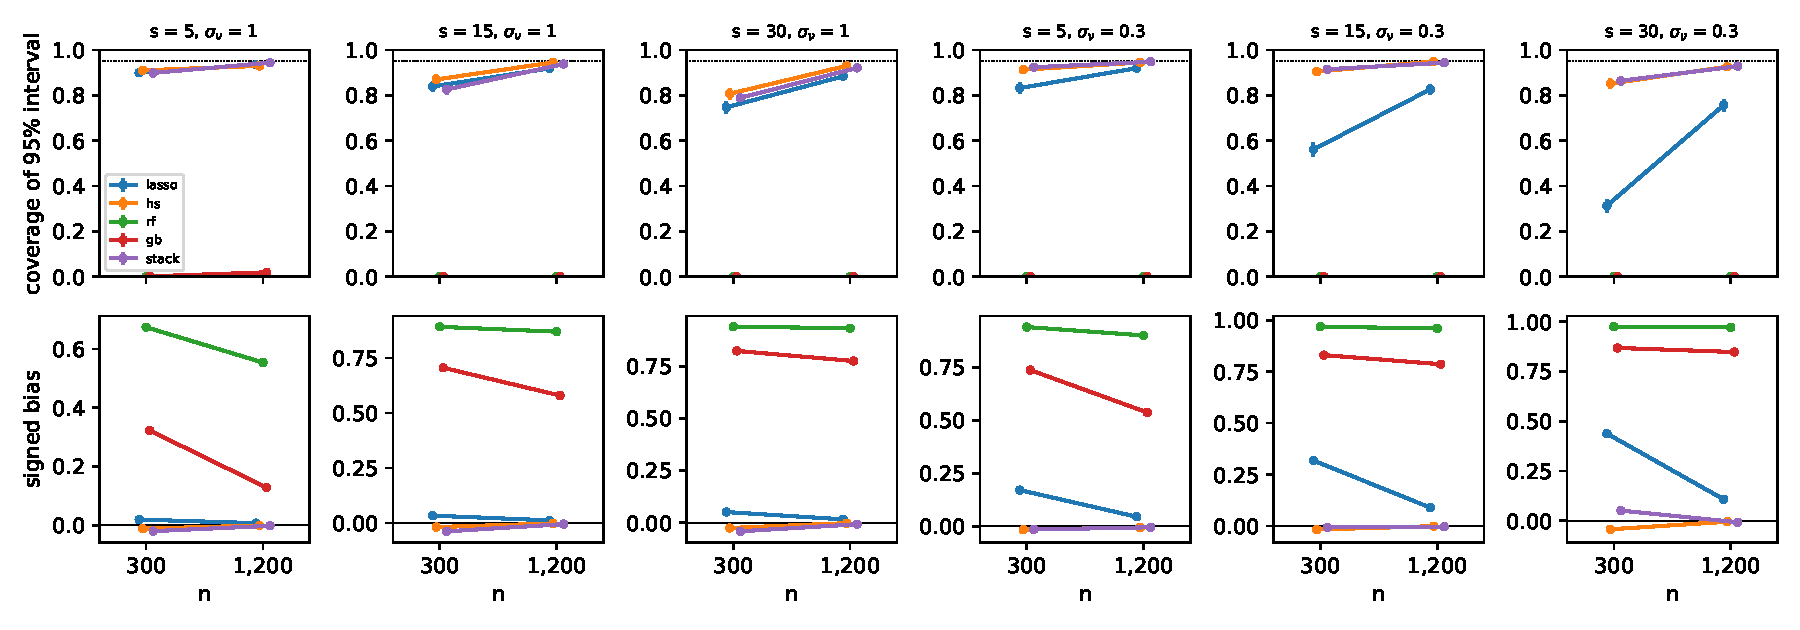
\includegraphics[width=\linewidth]{critique_learners.pdf}
\caption{Coverage of the nominal 95\% interval (top) and signed bias (bottom) of the cross fitted partially linear estimate at $n = 300$ and 1,200, by nuisance learner, with 95\% Monte Carlo intervals. Columns are $s = 5$, 15 and 30 at $\sigma_\nu = 1$ and then at $\sigma_\nu = 0.3$; $p = 400$, $\tau = 1$, five folds, 1,000 data sets per point, the same data sets for every learner.}
\label{fig:crit:learners}
\end{figure}

\section{What the reported standard error leaves out}\label{sec:crit:se}

Table~\ref{tab:crit:folds} compares five and two folds\index{cross fitting!number of folds|textbf} for the cross validated lasso on the same 5,000 data sets, with shared seeds and nothing else changed.

\begin{table}[ht]
\centering
\small
\caption{The fold count alone. DML with a cross validated lasso, $n = 300$, $p = 400$, $\tau = 1$, the same 5,000 data sets at five and at two folds, $s$ true confounders. Coverage is for nominal 95 percent intervals. The last two columns are the mean reported standard error and the Monte Carlo standard deviation of $\hat\tau$.}
\label{tab:crit:folds}
\begin{tabular}{@{}llrrrr@{}}
\toprule
$s$ & folds & coverage & bias & reported s.e. & s.d. of $\hat\tau$ \\
\midrule
5 & 5 & 0.917 & 0.017 & 0.0533 & 0.0586 \\
 & 2 & 0.865 & 0.023 & 0.0529 & 0.0654 \\
15 & 5 & 0.826 & 0.037 & 0.0523 & 0.0644 \\
 & 2 & 0.694 & 0.053 & 0.0513 & 0.0786 \\
30 & 5 & 0.734 & 0.050 & 0.0513 & 0.0734 \\
 & 2 & 0.450 & 0.106 & 0.0487 & 0.1265 \\
\bottomrule
\end{tabular}
\end{table}

Coverage\index{coverage}\index{coverage!of DML intervals} falls, which is no surprise: with fewer folds each nuisance is fitted on less data. McNemar's exact test gives $p = 3\times 10^{-30}$, $5\times 10^{-78}$ and $10^{-213}$. The columns to read are the last two. The reported standard error\index{standard error|textbf} falls by 0.7, 1.8 and 5.2 percent, while the Monte Carlo standard deviation of the estimator rises by 12, 22 and 72 percent. The ratio of reported error to spread goes from 0.91 to 0.81 at $s = 5$ and from 0.70 to 0.38 at $s = 30$, where the estimator becomes nearly three quarters again as variable and its interval gets narrower. The horseshoe nuisance shows the same thing: coverage falls from 0.928 to 0.577, from 0.895 to 0.587 and from 0.827 to 0.671 at $s = 5$, 15 and 30, and from 0.908 to 0.841 under weak overlap, as its spread rises by 142, 88, 24 and 27 percent against rises of 15, 9, 3 and 7 percent in its reported error. These are findings about two learners at $n = 300$ and $p = 400$ in linear designs. The change also cuts the training share of each fit from 80 to 50 percent, so the rise in spread mixes fold randomness with worse fits (the horseshoe arm's channels fall by factors of 5.5 and 7 when its fits use 240 observations and not 150). The cleaner statement concerns the reported standard error: when $K$ changes it moves by at most 5.2 percent for the lasso and 15 percent for the horseshoe, far less than the spread.

The lottery isolates the randomization\index{cross fitting!variance from the random split|textbf}. Hold one data set fixed ($s = 15$) and redraw only the fold assignment, 200 times at each of $K = 2$, 5 and 10. At $K = 5$ the estimates range from 0.932 to 1.069. Their standard deviation across assignments is 0.057, 0.026 and 0.019, against a reported standard error of 0.053 at all three fold counts. At five folds the randomization alone is half of what is reported, and at two folds it exceeds all of it. The horseshoe nuisance is no better: 0.102 at two folds against a reported 0.060, and 0.025 at five against 0.054. This data set's estimate happens to sit near the truth, so no five fold assignment rejects $\tau = 1$, and the number to read is the spread.

Real data show the same lottery. In the 401(k) data of Chapter~\ref{ch:k401}, repeating the five fold split gives lasso estimates from 9.52 to 10.26 thousand dollars over 20 partitions and forest estimates from 8.59 to 9.05 over 5, and Figure~\ref{fig:dmlsplits} draws every partition with its interval. The intervals are wide relative to the spread, so with the full sample the point estimate depends on a random seed without the conclusion changing. In our own extract of those data (a different set of 99 controls) the split to split standard deviation is a sixth of the reported standard error at $n = 9{,}915$ and two fifths in a random subsample of $n = 300$, where 200 fold assignments of that one data set return estimates between 1.90 and 26.22 thousand dollars.

\begin{figure}[ht]
\centering
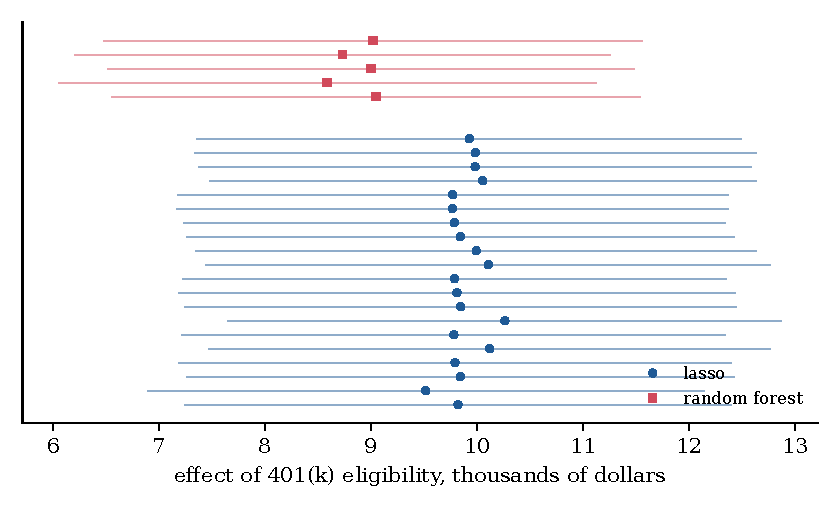
\includegraphics[width=0.9\linewidth]{dml_splits.pdf}
\caption{Cross fitted DML estimates of the effect of 401(k) eligibility on net financial assets, with 95\% intervals, for 20 random fold partitions with lasso nuisances and 5 with random forest nuisances.}
\label{fig:dmlsplits}
\end{figure}

Why the reported error barely responds to $K$ is a statement about what it conditions on. Fix fits $\eta = (\tilde m, \tilde\ell)$ and write $h_\eta = (T - \tilde m(X))(Y - \tilde\ell(X))$, $q_\eta = (T - \tilde m(X))^2$, $\tau_\eta = \E h_\eta/\E q_\eta$ and $\psi_\eta = (h_\eta - \tau_\eta q_\eta)/\E q_\eta$, the influence function, with expectations and variances below over one fresh observation. A direct calculation gives $\tau_\eta = \tau + \Delta(\eta)$, with $\Delta$ the bias of \eqref{eq:crit:bias} at the errors of $\eta$: $\Delta$ is the bias a fit carries and $\psi_\eta$ the noise around it. The cleanest statement is for a single split\index{cross fitting!single split|textbf}.

\begin{theorem}[What the sandwich sees, and what it cannot]\label{crit:thm:single}
Split the sample into a training part and an evaluation part of size $n_E \ge 17$\index{cross fitting!single split}, fit $\hat\eta = (\hat m, \hat\ell)$ on the training part alone, and compute the Robinson estimator $\hat\tau$ on the evaluation part. Assume the moment conditions and fourth moment bounds of Theorem~\ref{crit:thm:sharp} (and, for the bounds on $\tilde\delta_{n_E}$ and $R_{n_E}$ only, finite eighth moments of $\nu$ and $\varepsilon$ and $\E\delta_m^8 \le C\|\delta_m\|^8$, $\E\delta_\ell^8 \le C\|\delta_\ell\|^8$), that $\nu$ given $X$ has a bounded density, and that the fits satisfy $\|\delta_m\| + \|\delta_\ell\| \le 1$. Then $\E\hat\tau^2 < \infty$ and, conditionally on the training part,
\[
\E(\hat\tau \mid \hat\eta) = \tau + \Delta(\hat\eta) + \delta_{n_E}, \qquad \mathrm{Var}(\hat\tau \mid \hat\eta) = \frac{\mathrm{Var}(\psi_{\hat\eta})}{n_E} + \tilde\delta_{n_E},
\]
where $\|\delta_{n_E}\|_2 \le C_1/n_E$ and $\|\tilde\delta_{n_E}\|_1 \le C_2\,n_E^{-3/2}$, with constants that depend only on $J$, the moment bounds and the density bound. The sandwich variance estimator, which recentres at $\hat\tau$, estimates the leading term of the second display. Unconditionally, with $\sigma_\Delta^2 = \mathrm{Var}\{\Delta(\hat\eta)\}$,
\[
\mathrm{Var}(\hat\tau) = \frac{\E\,\mathrm{Var}(\psi_{\hat\eta})}{n_E} + \sigma_\Delta^2 + R_{n_E}, \qquad |R_{n_E}| \le \frac{2\sigma_\Delta C_1}{n_E} + \frac{C_1^2}{n_E^2} + \frac{C_2}{n_E^{3/2}}.
\]
Proof in Appendix~\ref{app:dmlproofs}.
\end{theorem}

The sandwich estimates the first term and misses the variance of bias across fits\index{standard error!what it leaves out|textbf}: one fit supplies one draw of $\Delta(\hat\eta)$, from which its variance cannot be estimated. This conditions on one fit; it gives no lower bound over all estimators and leaves open a bootstrap that refits the nuisance. The second term is negligible beside the first exactly when $\sqrt{n_E}\,\sigma_\Delta \to 0$, the rate condition for fluctuations rather than means. Under cross fitting, conditioning on all $K$ fits conditions on a statistic of every observation, because each fold trains the other fits. Only an identity survives.

\begin{proposition}[Cross fitting: the identity that survives]\label{crit:prop:cfvar}
Let $\hat\tau$ be the pooled cross fitted estimator\index{cross fitting!variance from the random split} with folds $I_1, \dots, I_K$ of sizes $n_k$ and fits $\hat\eta^{(-k)}$ that omit $I_k$. Set $\bar\Delta_n = \sum_k (n_k/n)\,b(\hat\eta^{(-k)})\big/\sum_k (n_k/n)\{J + \|\delta_m^{(k)}\|^2\}$, and $U_n = \hat\tau - \tau - \bar\Delta_n$. If $\hat\tau$ and $\bar\Delta_n$ are square integrable (the second holds when $\|\delta_m\| + \|\delta_\ell\| \le 1$ for every fit, since then $|\bar\Delta_n| \le \max(1, |\tau|)/J$) then\index{cross fitting!variance from the random split}
\begin{equation}
\mathrm{Var}(\hat\tau) = \mathrm{Var}(\bar\Delta_n) + 2\,\mathrm{Cov}(\bar\Delta_n, U_n) + \mathrm{Var}(U_n).
\label{eq:crit:cfvar}
\end{equation}
\end{proposition}
\begin{proof}
Write $\hat\tau - \tau = \bar\Delta_n + U_n$ and expand the variance of the sum.
\end{proof}

The sandwich is meant to estimate $\mathrm{Var}(U_n)$ by analogy with Theorem~\ref{crit:thm:single}; the identity does not establish that it does. If it does, it omits $\mathrm{Var}(\bar\Delta_n) + 2\,\mathrm{Cov}(\bar\Delta_n, U_n)$, whose cross term has no fixed sign. The paper's sufficient condition for a negligible cross term bounds how far one observation moves the fits. For the lasso in the worst case it requires $s\log p = o(\sqrt n)$; at $n = 300$, $p = 400$, $s = 5$, the two sides are about 30 and 17. Simulations know $\tau$ and both nuisances, so all four variance terms can be computed.

Take the simplest design in which they are computable, with no sparsity and no selection: $X \sim N(0, I_{20})$ with 20 irrelevant controls, treatment $T = \nu$ and outcome $Y = \tau T + \varepsilon$ with standard normal $\nu$ and $\varepsilon$ and $\tau = 1$, least squares nuisance fits, $n = 300$ and 30,000 replications. The cross term, as a multiple of $\mathrm{Var}(\bar\Delta_n)$, is $+0.02$ for a single split, which is zero within Monte Carlo error and consistent with the bound of Theorem~\ref{crit:thm:single}. Under cross fitting it is $+1.42$ at $K = 2$, $+0.21$ at $K = 3$, $-1.10$ at $K = 5$ and $-1.74$ at $K = 10$ (Exercise~\ref{ex:chcrit:7} checks the identity at $K = 5$). At two folds the omitted variance is two and a half times $\mathrm{Var}(\bar\Delta_n)$, and at five folds it is cancelled and reversed. Cross fitting induces a negative covariance between the realized bias and the noise around it, and $K$ is the dial. For a cross validated lasso at $p = 400$, with 2,000 replications a cell, the cross term at $K = 5$ is $-0.45$, $-0.39$, $-0.38$ and $-0.95$ times $\mathrm{Var}(\bar\Delta_n)$ at $s = 5$, 15, 30 and under weak overlap, four to eleven Monte Carlo standard errors from zero. At $K = 2$ and at a single split it is small and of either sign. In the dense design, where nothing covers, it stays within about two standard errors of zero at every fold count.

The omitted variance depends on $K$, while the reported error barely responds. Adding it closes only part of the gap: at $s = 30$ and five folds in the 2,000 replication run, adding $\mathrm{Var}(\bar\Delta_n) + 2\,\mathrm{Cov}(\bar\Delta_n, U_n) = 1.1\times 10^{-3}$ raises the reported error from 0.052 to 0.061 against a Monte Carlo spread of 0.073. The sandwich also falls short of $\mathrm{Var}(U_n)$, the block it should estimate: $2.7\times 10^{-3}$ against $4.2\times 10^{-3}$. We have no account of that gap.

Two procedures try to integrate over the fit, and they behave differently. The repeated split median of Chernozhukov and coauthors (2018), with the variance inflated by the spread across twenty splits, covers better than a single cross fit in all four designs where anything covers (Table~\ref{tab:crit:cmp}), at a cost of 3 to 11 percent in width, and moves the ratio of reported error to spread from 0.91, 0.81, 0.70 and 0.91 to 0.99, 0.93, 0.88 and 1.04. It repairs the variance and not the centre: under weak overlap coverage rises only from 0.557 to 0.603, because the error there is bias and the median of biased estimates is biased. The multiplier bootstrap\index{multiplier bootstrap|textbf} resamples the score at one fixed cross fit without refitting the nuisance (Mammen weights, 999 draws, percentile interval) and changes almost nothing: it covers 0.3 to 0.7 points below the single fit it resamples (McNemar $p$ of $2\times 10^{-4}$, 0.10, $9\times 10^{-4}$ and 0.004; Exercise~\ref{ex:chcrit:8}). Resampling the score is not integrating over the fit.

A bootstrap that does integrate over the fit is available at a price, and it overshoots. In a run of our own on 1,000 data sets per design ($n = 300$, $p = 400$, $\tau = 1$), we resampled the observations with replacement 499 times, refitted both cross validated lassos inside a fresh five fold cross fit in every resample, with all copies of an observation in the same fold and in the same inner validation fold, recomputed the estimate, and took the 2.5 and 97.5 percent points of the 499 estimates as the interval. On these data sets the single cross fit covers 0.916, 0.832 and 0.756 at $s = 5$, 15 and 30, and the refitting bootstrap 0.989, 0.998 and 0.984, with intervals 42, 70 and 126 percent wider: the mean squared bootstrap standard deviation is 1.7, 1.9 and 2.8 times the variance of the estimate across data sets. It is conservative, not calibrated. Under weak overlap it covers 0.607 against 0.536 for the single fit and 0.605 for the repeated split median, because the error there is bias, and in the dense design every procedure misses in every replication, with biases of 0.80 to 0.81 against mean interval widths of 0.16 to 0.30. There the bootstrap also understates the spread, with a mean squared standard deviation of $6.1\times 10^{-3}$ against a variance of $8.5\times 10^{-3}$.

\section{What no learner can repair}\label{sec:crit:repair}

Take eight equal strata of households, with propensities spaced evenly from 0.06 to 0.50 and effects from 2.0 down to 0. Give the partially linear score the true nuisance functions, so that no fitting error exists, and run it on $n = 4{,}000$ households for 500 replications. It returns 0.7701. The average effect is 1.0000. The interval covers 0.7706 on 0.960 of the replications and the average effect on none, and the gap does not shrink with $n$. The augmented score at the same true nuisances returns 0.9972 and covers the average effect on 0.966. Chapter~\ref{ch:dml} works this design by hand (Exercise~\ref{ex:chcrit:10} repeats the arithmetic), and Proposition~\ref{dml:prop:wate} explains the number: the weight $e(1 - e)$ is largest at a propensity of one half, so the stratum with the biggest effect and the weakest overlap gets the smallest weight. No learner can change that.

The weighting is not a defect in itself. Chapter~\ref{ch:dml} gives the case for choosing it, including trimming (Crump and coauthors 2009), and when the outcome variance is the same in both arms and at every covariate value, overlap weighting, whose weight is exactly $e(1 - e)$, has the smallest asymptotic variance among weighted average effects (Li, Morgan and Zaslavsky 2018). The objection is that DML arrives at this estimand silently: an analyst who calls a DML routine for the average treatment effect receives a different population without being told.

\paragraph{The efficiency bound and overlap.}\label{sec:dml:bound} Hahn (1998) gave the semiparametric efficiency bound\index{efficiency bound|textbf}\index{semiparametric efficiency bound|see{efficiency bound}} for the average effect. Write $\sigma_t^2(x) = \mathrm{Var}\{Y(t) \mid X = x\}$, $\tau(x) = \mu_1(x) - \mu_0(x)$ and $\bar\tau = \E\,\tau(X)$. The bound is
\begin{equation}
V_{\mathrm{eff}} = \E\left\{\frac{\sigma_1^2(X)}{e(X)} + \frac{\sigma_0^2(X)}{1 - e(X)} + \bigl(\tau(X) - \bar\tau\bigr)^2\right\}.
\label{eq:dml:bound}
\end{equation}
The first two terms are the outcome noise in each arm, inflated by the inverse probability of landing there, and they are what weak overlap does to any estimator of the average effect. In the example of Figure~\ref{fig:plmweights}, with $X \sim N(0,1)$, $\tau(x) = 1 + x$ and $e(x) = \expit(1 + \gamma x)$, the expectation $\E\{1/(1 - e(X))\}$ rises from 3.7 at $\gamma = 0$ to 246 at $\gamma = 3$, so with unit noise variances the best achievable variance rises about 46 times. The average effect is 1 for every $\gamma$, while the partially linear estimand is 0.70 at $\gamma = 1$, thirty percent lower, because the units it weights most, with propensity near one half, have below average effects. Whether a posterior attains the bound is a question about a Bernstein von Mises theorem for the average effect, taken up in Section~\ref{sec:crit:bayes} and in Appendix~\ref{app:theory}.

\begin{figure}[ht]
\centering
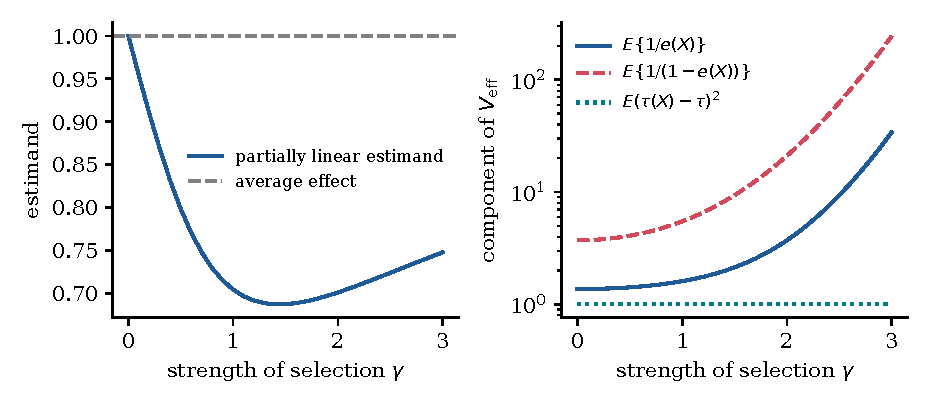
\includegraphics[width=\linewidth]{plm_weights.pdf}
\caption{Left: the partially linear estimand and the average effect as selection strengthens, for $\tau(x) = 1 + x$ and $e(x) = \expit(1 + \gamma x)$. Right: the three components of the efficiency bound \eqref{eq:dml:bound} with unit noise variances, on a log scale.}
\label{fig:plmweights}
\end{figure}

The Robinson denominator estimates $J$. At $J = 0$, $Y = \tau m(X) + g(X) + \varepsilon$, so any change in $\tau$ is absorbed by $g$ and the effect is unidentified. No procedure can approach this boundary safely\index{Dufour impossibility result|textbf}.

\begin{proposition}[No uniformly valid interval of finite length]\label{crit:prop:dufour}
Fix $n$. Let $\mathcal P$ be a class of laws of the partially linear model that contains, for each $j \in (0, \bar j\,]$ and each $\tau \in \mathbb R$, a law $P_{j,\tau}$ with $\E\,\mathrm{Var}(T \mid X) = j$ and effect $\tau$, and suppose that for every $L < \infty$
\[
\lim_{j \downarrow 0}\ \sup_{|\tau|, |\tau'| \le L}\ \bigl\|P_{j,\tau}^{\otimes n} - P_{j,\tau'}^{\otimes n}\bigr\|_{\mathrm{TV}} = 0.
\]
Let $\mathcal K_n$ be a confidence set with $\inf_{P \in \mathcal P} \Prob_P(\tau(P) \in \mathcal K_n) \ge 1 - \alpha$ for some $\alpha < 1$, whose graph is jointly measurable (as it is for any interval with measurable endpoints). Then $\sup_{P \in \mathcal P}\E_P\,\mathrm{Leb}(\mathcal K_n) = \infty$\index{Dufour impossibility result}. The Gaussian family $T = m(X) + \nu$, $\nu \sim N(0, j)$, $Y = \tau\nu + h(X) + \varepsilon$, $\varepsilon \sim N(0, \sigma_\varepsilon^2)$ satisfies the condition, with $\|P_{j,\tau}^{\otimes n} - P_{j,\tau'}^{\otimes n}\|_{\mathrm{TV}} \le L\sqrt{nj}/\sigma_\varepsilon$ for $|\tau|, |\tau'| \le L$. Proof in Appendix~\ref{app:dmlproofs}.
\end{proposition}

The proof is a Fubini argument in the manner of Gleser and Hwang (1987) and Dufour (1997): the expected length of $\mathcal K_n$ is the integral over $\tau'$ of the probability that it covers $\tau'$, and near $j = 0$ that probability is close to $1 - \alpha$ over a window as wide as one likes. The proposition carries two safeguards.

First, it does not contradict Chernozhukov and coauthors (2018), who fix $c > 0$ and require $\E\,\mathrm{Var}(T \mid X) \ge c$ throughout their class, on which the sandwich interval is uniformly valid. Here $J$ is positive at every law and has no common lower bound. That bound is an assumption, and the data cannot certify it.

Second, a fixed design cannot exhibit uniformity failure. The vanishing overlap sweep shows loss of calibration before the boundary. In our sweep ($s = 10$, five folds) the treatment residual standard deviation takes the values 1.0, 0.6, 0.35, 0.2 and 0.1. The width of the DML interval with a cross validated lasso rises by a factor of 10.1 and its bias from 0.034 to 0.907, a factor of 27, so coverage falls from 0.848 to 0.610. The reported error is right, with a ratio to the Monte Carlo spread between 0.85 and 1.05 down the sweep, and the centre is wrong. The deterioration belongs to the cross validated lasso. Post double selection at the theory penalty on the same data sets has bias $0.006$, $-0.006$ and $-0.033$ at residual standard deviations 0.35, 0.20 and 0.10, against 0.208, 0.428 and 0.907 for DML, with coverage 0.956, 0.946 and 0.972 against 0.704, 0.626 and 0.610, and a horseshoe nuisance at five folds does not show the deterioration either. The theory penalty succeeds only where it recovers the support, which it does on 1,493 of 1,500 fits at $s = 10$ and on none at $s = 30$, and no data driven check separates the two cases.

The Bayesian analogue is not exempt: a credible set of finite expected length over the same class is not uniformly valid either. In the same sweep the reduced form posterior of Section~\ref{sec:crit:bayes} widens from 0.247 to 2.631 and its coverage rises from 0.806 to 0.970, while DML's falls. Both intervals widen by about the same factor, 10.1 for DML and 10.7 for the posterior. What separates them is the centre: the bias grows 27 times for DML and 1.9 times for the posterior, from 0.068 to 0.126.

\begin{remark}[No certificate]\label{crit:rem:cert}
The bias functional $b$ is a combination of an inner product and a squared norm of the unknown nuisance errors. Certifying the rate condition therefore means estimating those two functionals. In the regime $s \gg \sqrt n/\log p$ the minimax rate for functionals of this kind is of order $s\log p/n$ (Guo, Wang, Cai and Li 2019), which is the order of $b$ itself, and the impossibility of adaptive confidence intervals (Cai and Guo 2017) is the same phenomenon one level down. This is an argument and not a theorem, since no matching lower bound for the composite functional is proved. For smooth nuisance functions the barrier is known: root $n$ estimation of the average effect needs roughly $\beta_e + \beta_\mu \ge d/2$, for propensity and outcome smoothness $\beta_e$ and $\beta_\mu$ in dimension $d$, and below that no interval of width $O(n^{-1/2})$ is valid (Robins, Tchetgen Tchetgen, Li and van der Vaart 2009; Robins, Li, Mukherjee, Tchetgen Tchetgen and van der Vaart 2017; Balakrishnan, Kennedy and Wasserman 2023).
\end{remark}

No general test of the rate condition is known. Unconfoundedness and no interference cannot be tested from observational data. If unconfoundedness fails, the average effect lies in a set whose size depends on the failure (Manski 1990); DML maintains the assumption and reports a point, saying nothing about that set. A Bayesian prior states how strongly an unmeasured confounder might act and visibly carries the unidentified part (Chapter~\ref{ch:tianpearl}).

\section{The same anatomy in weighting}\label{sec:crit:weights}

Replace the partially linear score by the augmented score \eqref{eq:aipw} of Chapter~\ref{ch:dml} and the estimand problem goes away. The error problem does not. With $\hat e$ and $\hat\mu_t$ the fitted propensity and arm regressions, the mean of the score at the fitted nuisances, derived there, is a sum of two products of the propensity error with the outcome error in each arm.
Each term is bounded by a Cauchy and Schwarz product, and the alignment question returns, since a covariate that raises the propensity usually raises the outcome too. Polson and Sokolov (2026b) state that the sharp rate condition transfers to this score with a weighted cosine between the propensity error and the outcome errors and a factor $1/\hat e_{\min}$ in the bound, where $\hat e_{\min}$ is the smallest value of $\hat e(x)$ and $1 - \hat e(x)$, so that weak overlap multiplies the alignment penalty instead of acting separately from it. The proof is in their supplement and is not reproduced here.

The augmented score is doubly robust\index{double robustness}: it is consistent if either the propensity or the outcome model is correct (Robins, Rotnitzky and Zhao 1994). Three qualifications apply. Both models can be wrong: in high dimensions both are approximations and the guarantee is silent, and when both are moderately wrong the estimator can be worse than regression adjustment alone, because the weighting term amplifies the outcome model's errors where the estimated propensity is small (Kang and Schafer 2007; Chapter~\ref{ch:ipw}). The guarantee is asymptotic, and in finite samples, especially with propensities near zero or one, the remainder terms can dominate. And a posterior does not become doubly robust by being Bayesian. It can put a direction for the propensity score into its prior, as the Bayesian causal forest and the coupled horseshoe of Chapter~\ref{ch:horseshoe} do, which lowers its sensitivity to confounding in that direction. Bayesian AIPW, in the same chapter, combines a posterior with the augmented score explicitly and inherits double robustness from the score.

\section{Where Bayes helps and where it does not}\label{sec:crit:bayes}

Suppose the analyst, persuaded by the last four sections, writes the Bayesian analysis a well trained Bayesian would write: $Y = \tau T + X^\top\beta + \varepsilon$, a horseshoe prior on $\beta$ and a flat prior on $\tau$. At $s = 30$ confounders ($n = 300$, $p = 400$) its posterior mean averages 1.96 for a true effect of 1, its 95 percent interval is 0.073 wide, and the interval covers the truth in none of 5,000 replications\index{credible interval!frequentist coverage of|textbf}\index{coverage!frequentist, of credible intervals|textbf}. The DML arms report intervals about 0.2 wide. The failure has a name and a limit.

\begin{proposition}[Complete shrinkage bias]\label{crit:prop:ric}\label{crit:prop:default}
Let $T = X^\top\gamma + \nu$ and $Y = \tau T + X^\top\beta + \varepsilon$, with $\E X = 0$, $\mathrm{Var}(X) = \Sigma$, $\E \nu = 0$, $\mathrm{Var}(\nu) = \sigma_\nu^2$, $\nu$ uncorrelated with $X$ and $\E(\varepsilon \mid T, X) = 0$ with $\E \varepsilon^2 < \infty$. Shrinking $\beta$ entirely to zero\index{default prior} and regressing $Y$ on $T$ alone converges in probability, under independent sampling as $n \to \infty$, to
\[
\tau_\infty = \tau + \frac{\gamma^\top\Sigma\beta}{\gamma^\top\Sigma\gamma + \sigma_\nu^2}.
\]
If $\Sigma = I_p$ and $\gamma_j = \beta_j = c \ne 0$ on a set of size $s$ and zero elsewhere, the bias is $sc^2/(sc^2 + \sigma_\nu^2)$, which increases in $s$ and tends to one.
\end{proposition}
\begin{proof}
Since $\E(\varepsilon T) = 0$, the univariate coefficient converges to
\[
\frac{\mathrm{Cov}(T,Y)}{\mathrm{Var}(T)} = \tau + \frac{\gamma^\top\Sigma\beta}{\gamma^\top\Sigma\gamma + \sigma_\nu^2}.
\]
With $\Sigma = I_p$ and the stated coefficients, both quadratic forms equal $sc^2$.
\end{proof}

The limit is omitted variable bias\index{omitted variable bias}, the bias when shrinkage is complete. In the symmetric design, dropping $k$ of the $s$ confounders and keeping the rest gives the smaller bias $kc^2/(kc^2 + \sigma_\nu^2)$, so there no selection does worse than dropping them all. In other designs the limit is not a ceiling: with $\Sigma = I_2$, $\gamma = (1, 1)^\top$, $\beta = (1, -1)^\top$ and $\sigma_\nu = 1$, complete shrinkage has no bias, while dropping the first confounder alone leaves a bias of $1/2$. As the prior pulls $\beta$ toward zero, the treatment coefficient, the only unpenalized parameter, absorbs the confounding that the shrunken coefficients no longer explain, which is regularization induced confounding\index{regularization induced confounding} (Hahn, Carvalho, Puelz and He 2018). The sampling variance of the misspecified regression is of order $1/(ns)$ in this design, so the interval narrows as the bias grows. At $c = \sigma_\nu = 1$ the limiting bias is 0.83, 0.94 and 0.97 at $s = 5$, 15 and 30. The naive Bayes biases in our designs are 0.032, 0.362 and 0.956, about 4, 39 and 99 percent of the limit, and the interval widths are 0.224, 0.490 and 0.073 (at $s = 15$ the posterior has two modes, near 1 and near 2, and the pooled interval spans both when the chains of a replication disagree): the posterior is most confident where it is most wrong. In this design the limit is a ceiling and not a prediction for finite $n$. The harm comes from applying a prior chosen for its estimation properties in coordinates that ignore the design, and the reduced form below applies the same family of prior to different coefficients.

The remedy is a change of coordinates. Following DiTraglia and Liu (2025), put horseshoe priors on the coefficients of the two nuisance regressions, $m(x) = x^\top\gamma$ and $\ell(x) = x^\top\varsigma$ with $\varsigma = \tau\gamma + \beta$, instead of on the structural coefficient $\beta$. Chapter~\ref{ch:horseshoe} takes the other route and couples the two regressions in the structural coordinates. Table~\ref{tab:crit:head} gives three of our five designs.

The reduced form model is $T = X\gamma + \nu$ and $Y = X\varsigma + \tau\nu + \varepsilon$, with $\nu \sim N(0, \sigma_\nu^2 I)$ and $\varepsilon \sim N(0, \sigma_\varepsilon^2 I)$ independent and $\varsigma = \tau\gamma + \beta$. The prior is a horseshoe on $\gamma$ with scales proportional to $\sigma_\nu$ and a horseshoe on $\varsigma$ with scales proportional to $\sigma_\varepsilon$, each with its own half Cauchy local and global scales, a flat prior on $\tau$ and Jeffreys priors on the two variances, and the sampler is Gibbs. Given a nuisance draw $\eta = (\gamma, \varsigma, \sigma_\nu, \sigma_\varepsilon)$, let $\nu_\gamma = T - X\gamma$ and $r_\varsigma = Y - X\varsigma$. The effect is then normal with mean $a_\eta = \nu_\gamma^\top r_\varsigma/\nu_\gamma^\top\nu_\gamma$ and variance $V_\eta = \sigma_\varepsilon^2/\nu_\gamma^\top\nu_\gamma$, a Robinson regression at the drawn nuisance. By the law of total variance, $\mathrm{Var}(\tau \mid D) = \E(V_\eta \mid D) + \mathrm{Var}(a_\eta \mid D)$. The first term plays the part of the sandwich, and the second is the spread of the centre across nuisance draws, the posterior counterpart of $\sigma_\Delta^2$ in Theorem~\ref{crit:thm:single}. The two are not shown to be equal, since one is a posterior spread and the other a frequentist variance.

\begin{table}[ht]
\centering
\small
\caption{Head to head in three of our five designs. $n = 300$, $p = 400$, $\tau = 1$, nominal 95 percent intervals, seeds shared across arms; 5,000 replications a cell in the sparse and weak overlap blocks (the data sets of Table~\ref{tab:dml:sims}) and in the dense block 4,406 for the lasso row, 5,000 for the horseshoe rows and 1,000 for naive Bayes and the posterior. In the sparse and weak overlap blocks the reduced form posterior and naive Bayes run four chains of 10,000 sweeps per replication, doubled until split $\hat R$ for $\tau$ is at most 1.01 and its effective sample size at least 400, up to 80,000 sweeps a chain; every reduced form replication passed, naive Bayes at $s = 15$ in 59 percent, because its posterior there has two modes. The horseshoe nuisance is the posterior mean from 1,200 sweeps. DML rows carry their fold count; the reduced form posterior is the default Bayes arm. The last two columns divide the mean reported standard error by the Monte Carlo standard deviation of the estimator and by its root mean squared error. The dense posterior row uses four chains per replication, run until split $\hat R$ for $\tau$ is at most 1.01 and its effective sample size at least 400, which took up to 800,000 sweeps a chain; 103 of the 1,000 replications had not passed by then and 7 that passed report a standard error above 1, and the row is over the other 890.}
\label{tab:crit:head}
\begin{tabular}{@{}lrrrr@{}}
\toprule
 & bias & coverage & s.e./s.d. & s.e./RMSE \\
\midrule
\multicolumn{5}{@{}l}{\textit{sparse, $s = 15$}} \\
DML, lasso, $K = 5$ & 0.037 & 0.826 & 0.81 & 0.70 \\
DML, horseshoe, $K = 5$ & $-0.012$ & 0.895 & 0.85 & 0.83 \\
DML, horseshoe, $K = 2$ & $-0.069$ & 0.587 & 0.49 & 0.43 \\
naive Bayes & 0.362 & 0.446 & 0.56 & 0.36 \\
reduced form posterior & 0.076 & 0.787 & 1.02 & 0.66 \\
\addlinespace
\multicolumn{5}{@{}l}{\textit{weak overlap, $s = 15$, $\sigma_\nu = 0.3$}} \\
DML, lasso, $K = 5$ & 0.317 & 0.557 & 0.91 & 0.47 \\
DML, horseshoe, $K = 5$ & $-0.024$ & 0.908 & 0.87 & 0.86 \\
DML, horseshoe, $K = 2$ & $-0.040$ & 0.841 & 0.74 & 0.73 \\
naive Bayes & 0.987 & 0.000 & 0.48 & 0.02 \\
reduced form posterior & 0.148 & 0.906 & 1.01 & 0.85 \\
\addlinespace
\multicolumn{5}{@{}l}{\textit{dense confounding}} \\
DML, lasso, $K = 5$ & 0.799 & 0.000 & 0.46 & 0.05 \\
DML, horseshoe, $K = 5$ & 0.677 & 0.000 & 0.56 & 0.09 \\
DML, horseshoe, $K = 2$ & 0.783 & 0.000 & 0.54 & 0.06 \\
naive Bayes & 0.935 & 0.000 & 0.99 & 0.02 \\
reduced form posterior & 0.938 & 0.000 & 1.30 & 0.03 \\
\bottomrule
\end{tabular}
\end{table}

The ratio of reported error to spread is the column to read first, because it is the one Theorem~\ref{crit:thm:single} is about. The reduced form posterior reports 1.05, 1.02, 1.00 and 1.01 of its own spread at $s = 5$, 15, 30 and under weak overlap, with converged chains in every one of the 5,000 replications. DML with the cross validated lasso at five folds reports 0.91, 0.81, 0.70, 0.91 and 0.46 at $s = 5$, 15, 30, under weak overlap and in the dense design, and with a horseshoe nuisance 0.95, 0.85, 0.73, 0.87 and 0.56, falling to between 0.45 and 0.74 at two folds. This is the one place where the evidence is unambiguous: a posterior over the nuisance pair integrates over the fit by construction, and its reported error does not omit the dispersion term. It is no certificate. In the dense design, where every coordinate is nonzero and no learner makes the nuisance error vanish, the posterior reports 1.30 times its spread, is biased by 0.94 and covers in none of the 890 replications of the table. In 103 of the 1,000 its four chains, started from widely dispersed values, had not converged after 800,000 sweeps, and their intervals are so wide (median width 175) that 71 of them cover; 7 more converged with standard errors from 1.25 to 610, and the table leaves all 110 out. The ratio that governs coverage is the last column, reported error over root mean squared error, and it is 0.03 there.

On the estimate itself the picture is mixed, and DML wins the sparse designs. Its bias at $s = 5$, 15 and 30 is 0.017, 0.037 and 0.050 against 0.041, 0.076 and 0.106 for the posterior, paired differences of 0.025, 0.039 and 0.056, each more than 60 standard errors from zero. Coverage separates them at $s = 15$ and 30 and not at $s = 5$: 0.917, 0.826 and 0.734 against 0.913, 0.787 and 0.704 (McNemar $p$ of 0.25, $4\times 10^{-13}$ and $6\times 10^{-6}$), and both fall well below nominal by $s = 30$. Under weak overlap\index{overlap!weak} the order reverses: the posterior covers on 0.906 of the replications against 0.557, on 1,776 discordant pairs to 30. DML with a horseshoe nuisance at five folds is the best centred arm, with absolute bias 0.011, 0.012, 0.021 and 0.024 in the four designs where anything covers. Its coverage, 0.928, 0.895, 0.827 and 0.908, is above the lasso arm's in all four designs (McNemar $p = 0.008$ at $s = 5$ and below $10^{-27}$ in the other three) and above the posterior's by 1.5, 10.8 and 12.4 points at $s = 5$, 15 and 30 ($p = 0.001$ and below $10^{-45}$), and under weak overlap it matches the posterior, 0.908 against 0.906 ($p = 0.74$). Cutting its folds to two cuts its coverage to 0.577, 0.587, 0.671 and 0.841. In the dense design, where nothing covers (Table~\ref{tab:crit:head}), no interval should be reported.

To separate DML from the cross validated lasso inside it, Table~\ref{tab:crit:cmp} runs four more procedures on the same data sets by seed replay.

\begin{table}[ht]
\centering
\small
\caption{Four more procedures on the data sets of Table~\ref{tab:crit:head} ($n = 300$, $p = 400$, $\tau = 1$; the dense design is omitted), replayed on the same seeds. The first row is DML with the cross validated lasso at five folds. Post double selection refits least squares on the union of the variables chosen by lasso regressions of the outcome and of the treatment on the controls, with the lasso penalty set by theory or by cross validation. The repeated split median and the multiplier bootstrap are the two procedures of Section~\ref{sec:crit:se}. Nominal 95 percent intervals, 5,000 replications a cell.}
\label{tab:crit:cmp}
\begin{tabular}{@{}lrrr@{}}
\toprule
 & bias & coverage & mean width \\
\midrule
\multicolumn{4}{@{}l}{\textit{sparse, $s = 5$}} \\
DML, cross validated lasso & 0.017 & 0.917 & 0.209 \\
post double selection, theory penalty & $-0.002$ & 0.950 & 0.216 \\
post double selection, CV penalty & $-0.086$ & 0.669 & 0.249 \\
repeated split median & 0.017 & 0.936 & 0.215 \\
multiplier bootstrap & 0.017 & 0.911 & 0.208 \\
\addlinespace
\multicolumn{4}{@{}l}{\textit{sparse, $s = 15$}} \\
DML, cross validated lasso & 0.037 & 0.826 & 0.205 \\
post double selection, theory penalty & 0.798 & 0.010 & 0.127 \\
post double selection, CV penalty & $-0.110$ & 0.629 & 0.285 \\
repeated split median & 0.038 & 0.870 & 0.218 \\
multiplier bootstrap & 0.037 & 0.823 & 0.204 \\
\addlinespace
\multicolumn{4}{@{}l}{\textit{sparse, $s = 30$}} \\
DML, cross validated lasso & 0.050 & 0.734 & 0.201 \\
post double selection, theory penalty & 0.960 & 0.000 & 0.066 \\
post double selection, CV penalty & $-0.120$ & 0.651 & 0.337 \\
repeated split median & 0.051 & 0.820 & 0.224 \\
multiplier bootstrap & 0.050 & 0.728 & 0.200 \\
\addlinespace
\multicolumn{4}{@{}l}{\textit{weak overlap, $s = 15$, $\sigma_\nu = 0.3$}} \\
DML, cross validated lasso & 0.317 & 0.557 & 0.687 \\
post double selection, theory penalty & 0.924 & 0.034 & 0.138 \\
post double selection, CV penalty & $-0.134$ & 0.867 & 0.925 \\
repeated split median & 0.316 & 0.603 & 0.723 \\
multiplier bootstrap & 0.317 & 0.550 & 0.684 \\
\bottomrule
\end{tabular}
\end{table}

Post double selection\index{double selection|textbf} (Belloni, Chernozhukov and Hansen 2014) at the theory penalty is the best procedure in the table at $s = 5$, with bias $-0.002$ and coverage 0.950 against DML's 0.917 (McNemar $p = 2\times 10^{-20}$). At $s = 15$ and $s = 30$ it fails completely, with biases of 0.798 and 0.960, because the theory level is calibrated to a sparsity the design does not have and the joint lasso keeps 8.9 and 2.2 coordinates. At the cross validated penalty it keeps 37.8, 89.4 and 146.3 coordinates and covers below DML in all three sparse designs. Which tuning is good depends on the sparsity, which the data cannot certify. Under weak overlap post double selection at the cross validated penalty covers on 0.867 against DML's 0.557 and below the posterior's 0.906 (McNemar $p = 5\times 10^{-10}$), while DML with a horseshoe nuisance matches the posterior, so the weak overlap result is a statement about the cross validated lasso inside the score more than about Bayes against frequentism. The reduced form posterior's lowest coverage in these four designs is 0.704, against 0.557 for DML, 0.000 for post double selection at the theory penalty, 0.629 at the cross validated penalty, 0.603 for the repeated split median\index{cross fitting!repeated splits} and 0.550 for the multiplier bootstrap\index{multiplier bootstrap}. Post double selection at the theory penalty is ahead of the posterior at $s = 5$ and far behind it at the other three designs, while DML and the repeated split median cover at least as well as the posterior at $s = 5$, 15 and 30 and worse under weak overlap. Which case applies turns on sparsity and overlap, which the data do not reveal, so the argument is about worst cases and not about averages. Only DML with a horseshoe nuisance at five folds, whose lowest coverage is 0.827, does better in the worst case, and it costs 19.1 seconds a data set.

Cross fitting the reduced form posterior makes it worse. Coverage in the four designs where anything covers falls from 0.913, 0.787, 0.704 and 0.906 for the pooled posterior on 5,000 replications to 0.737, 0.351, 0.066 and 0.754 at five folds, on 4,976, 4,991, 4,999 and 5,000 replications. Each fold's posterior is sampled by four chains, the held out estimate is combined across the folds at every draw, and the four chain rule of Table~\ref{tab:crit:head} is applied to that combined estimate; it passes in 88, 98, 98 and 99.5 percent of the replications, so the first figure is the least secure. At two folds the sampler mixes far more slowly. With four chains per fold from overdispersed starts, $\tau$ drawn jointly with $\varsigma$, and 100,000 sweeps doubled up to 800,000, on 500 replications per design, coverage is 0.55, 0.04, 0.01 and 0.33, and the chains pass the same rule in 466, 292, 494 and 307 of the 500. At $s = 15$ and under weak overlap about two replications in five have not converged, so those two coverages pool converged and unconverged chains, and any of the four carries a Monte Carlo standard error of up to 0.022. The direction is not in question: the cross fitted posterior is biased downward in every design, by 0.08 to 0.24 at five folds and by 0.12 to 0.45 at two, and in the replications whose chains converged as well. The pooled posterior's small bias is a cancellation between a negative pure bias term and a positive dependence term, and there is no argument for why the two should track. Its bias is positive in every design, so the mechanism of Proposition~\ref{crit:prop:ric} survives the change of coordinates in weakened form. Its centring in these designs is an empirical finding with no theorem behind it.

The orthogonal score is the efficient score for $\tau$ in the partially linear model when the outcome noise is homoskedastic (otherwise efficiency needs variance weights), and the augmented score is the efficient influence function for the average effect. A Bayesian model can share their first order behaviour when its prior contains the direction those scores use, the propensity score\index{propensity score}. Ray and van der Vaart (2020) prove a semiparametric Bernstein von Mises theorem\index{Bernstein von Mises theorem} for the mean of a binary outcome missing at random, one arm of an average effect, under smoothness conditions that weaken when the Gaussian process prior includes a component in that direction (Appendix~\ref{app:theory} states the scope), and the coupled horseshoe of Chapter~\ref{ch:horseshoe} and the Bayesian causal forest of Hahn, Murray and Carvalho (2020) put the propensity into the prior for the same reason. We prove nothing of the kind for the horseshoe, and the measurements above are the evidence we have: modelling the treatment equation together with the outcome, as the reduced form does, shrinks the regularization induced confounding of Proposition~\ref{crit:prop:ric} without ending it. Orthogonality is a property a Bayesian model can aim at by construction, and a posterior adds the rest of the distribution.

Cheapness is the one advantage we grant DML without qualification. In a one core timing run of our own ($n = 300$, $p = 400$, ten data sets of the $s = 15$ design), a cross fitted lasso took 1.0 seconds on average against 9.8 for one chain of 2,000 sweeps of the reduced form sampler, and it needs no convergence diagnostics, though the analyst still chooses the score, the learners, their tuning and the folds. The cheapness belongs to the lasso and not to the template: DML with a horseshoe nuisance at five folds took 19.1 seconds. The posterior of Table~\ref{tab:crit:head} runs four chains and extends them until they pass the convergence checks, which took 194 to 227 seconds, about 200 times the lasso; naive Bayes took 96 seconds on seven of the data sets and about 1,440 on the other three.

\paragraph{What four people get.}\label{sec:crit:applied} The case for a posterior rests less on the point estimate of an average effect than on what a decision needs. Under the model, and with a prior the analyst can defend, one fit supplies each of the following; a DML analysis would need a separate score for each, and none of them comes out as a probability. A regulator gets the probability that the effect exceeds a clinically meaningful threshold, the effect in each prespecified subgroup and a predictive distribution for the next patient. A ministry with a fixed budget needs the conditional effect for each household to rank them, its uncertainty to avoid chasing noise, and the distribution of gains to judge equity. In the 401(k) data of Section~\ref{sec:deephd} one quantile network, refitted 200 times under Bayesian bootstrap weights, gives the effect in every income quintile, from about three thousand dollars to eighteen, and the whole conditional distribution of assets behind each. DML with the augmented score also gives quintile effects from one set of nuisance fits (Chapter~\ref{ch:k401}), but not the distributions. A court asks whether this plaintiff's cancer was caused by smoking, a probability of causation that data bound but do not identify; the answer is a posterior inside the bounds with its prior stated, and DML has no object here, since no average identifies a probability that concerns one person (Chapter~\ref{ch:tianpearl}). An economist modelling a merger needs the price effect as a function of demand elasticities, conduct and costs, and then the probability that prices rise by more than a competition authority's threshold (Chapter~\ref{ch:blp}); a point estimate with a standard error is where that calculation starts. The analyst pays with a model and a prior. The predictive check of Chapter~\ref{ch:k401} shows replicated 401(k) wealth from a Gaussian outcome model to be far too symmetric, while a Student $t$ error model with three degrees of freedom reproduces the bulk of the data much better. The prior must put the design in, or regularization induced confounding returns. DML has assumptions of its own, and none of them appears in its output.

\section{Three real data sets}\label{sec:crit:real}



\paragraph{401(k) eligibility.} The 1991 SIPP extract of Chernozhukov and Hansen (2004) has $n = 9{,}915$, eligibility as the treatment, net financial assets as the outcome and, in our basis, $p = 99$ controls (not the basis of Chapter~\ref{ch:k401}). Nine procedures that disagree sharply in the simulations, all built on the Gaussian partially linear score, return between 9.41 and 10.67 thousand dollars, a spread of 1.26, which is 0.94 of one least squares standard error. This is the regime DML was built for: $p/n$ is 0.01, the treated fraction is 0.37, and the mean squared treatment residual is 0.196, nowhere near zero. In this regime DML is a good choice and this chapter does not argue otherwise. The agreement is within a family, though. Three procedures that change the score or the likelihood give 5.81 (a Student $t$ outcome likelihood with four degrees of freedom, whose interval is 1.47 wide against 4.67 for the Gaussian one, which returns 9.56), 8.34 (the augmented score, standard error 1.31) and 7.16 (a stratified horseshoe over deciles of an estimated propensity, standard error 1.23). The $t$ likelihood estimates a robust centre and not a mean, and net financial assets have skewness 10.6 and excess kurtosis 184, so these three do not estimate the same functional as the nine. The three sit 1.1 to 3.6 thousand dollars below the lowest of the nine, which span 1.26 among themselves.

\paragraph{LaLonde.} LaLonde (1986) asked whether observational estimators recover the experimental effect of the National Supported Work demonstration when the randomized controls are replaced by a survey comparison group. We use the 185 treated units of the Dehejia and Wahba (1999) sample against the 2,490 units of the PSID comparison group, with ten covariates expanded to $p = 56$ terms, and three truths: the experimental effect on the treated, 1.79 thousand dollars, and zero for each of two placebos (the 260 randomized controls in place of the treated, and 1975 earnings as the outcome with the 1975 covariates withheld). Every procedure built on the partially linear score returns between $-0.23$ and $0.46$ against 1.79. We read this as the overlap weighted estimand of Proposition~\ref{dml:prop:wate}, since most treated units have propensities near one, where $\mathrm{Var}(T \mid X)$ is smallest. On the real data that reading cannot be separated from confounding. Every procedure, Bayesian or not, fails the placebo by between 2.4 and 7.3 thousand dollars, which suggests that the PSID comparison is not ignorable given the available covariates (Smith and Todd 2005 revisit the sensitivity of such comparisons), so the gap mixes the estimand with the failure of identification. Only a semi synthetic version of the design separates them. It keeps the real covariates of the 2,675 units and simulates the rest in 100 replications: treatment is Bernoulli with the propensity $e$ of a ridge logistic regression of the real treatment on the expanded basis, redrawn every replication; the untreated outcome is a gradient boosting\index{gradient boosting|textbf} fit (depth 3, 300 trees) of real 1978 earnings on the ten main covariates among the 2,490 comparison units, plus noise resampled from those units' residuals; and the effect is $1.794 + 1.5\{e(x) - \bar e_T\}$ with $\bar e_T = \E e^2/\E e$, so that the expected effect on the treated is the experimental benchmark and the effect rises with the propensity. There the partially linear DML rows cover the overlap weighted effect they target (1.31 in that design) on 0.94 of replications and the effect on the treated on 0.87. On real data the structural assumption fails before the estimator does.

\paragraph{IHDP.} Hill (2011) removed the treated children of nonwhite mothers from the Infant Health and Development Program\index{Infant Health and Development Program}, which leaves 747 children of whom 139 are treated and makes overlap incomplete by construction, kept the 25 real covariates and the real treatment, and simulated outcomes from Hill's linear surface: in each replication the untreated outcome is $b_0 + X^\top b$ plus standard normal noise, with $b_0$ drawn uniformly from $\{0, 1, 2, 3, 4\}$ and each of the 25 slopes drawn from the same five values with probabilities 0.5, 0.125, 0.125, 0.125 and 0.125, and the treated outcome adds a constant effect of 4 and its own standard normal noise. The target is the effect on the treated, 4 in every replication, and the setting is 100 replications. The partially linear DML score covers in none of them. The effect is constant, so every weighted average of it is 4 and Proposition~\ref{dml:prop:wate} is not the explanation. The mechanism of Theorem~\ref{crit:thm:atten} fits what follows, although its hypotheses are not checked here: the treatment is binary, so its residual variance is not constant in $X$, and nothing shows the cross channel to be negligible. In a separate run of 12 replications at effects of 0, 4 and 8, the estimate at 4 and 8 is 0.78 and 0.79 of the truth, and with an effect of zero there is nothing to attenuate. In another, of 20 replications, replacing the outcome learner by a post lasso refit, or by least squares on any of three bases, leaves the bias between $-0.88$ and $-1.12$. In the 12 replication run, replacing the cross validated $\ell_1$ logistic propensity on a 160 column basis by an unpenalized logistic on the 25 main effects removes almost all of it and leaves a ratio of 0.98. Cross validation shrank the propensity toward its mean, the error it left entered the treatment residual as measurement error, and the estimator returned the reliability ratio\index{reliability ratio} times the effect. Its own denominator reports the ratio: $\hat J_n$ is 0.180 under the penalized propensity and 0.147 under the unpenalized one, so if the second is close to $J$ the representation predicts $0.147/0.180 = 0.82$ against the 0.78 observed. This reads as the own square channel binding with the outcome regression essentially exact, and it is invisible from inside the procedure: the reported standard error is 1.07 times the estimator's spread, and the interval is centred at 3.12.

The Bayesian side has one resolved gain and one resolved loss. In the semi synthetic LaLonde design two posteriors for the effect on the treated, one from an outcome model with the propensity as a covariate and one from a prior that is exchangeable within propensity strata, cover at 0.97 and 0.99 against 0.88 for the doubly robust DML interval (exact McNemar $p = 0.022$ and $0.003$), on intervals a third wider and with no resolved difference in root mean squared error. On IHDP the procedures that target the effect on the treated are all accurate and 100 replications do not separate them, with one exception that runs against default Bayes, the reduced form posterior with the binary treatment treated as Gaussian: on the linear surface it covers at 0.90 and the doubly robust DML interval at 0.97 (exact McNemar $p = 0.039$).

\section{What this chapter does not establish}\label{sec:crit:limits}

The critique is theoretical and the evidence is simulated, and the gap between the two is where a reader should press. The designs are linear and Gaussian, with $n = 300$ and $p = 400$. The paper runs a cross validated lasso, a theory penalty lasso in one experiment and a horseshoe posterior mean inside DML; our forest, boosting and stack comparison uses one law that favours linear learners. Neural networks, propensity calibration, BART on IHDP and a binary treatment model inside the reduced form sampler are untried. The 5,000 replication comparisons have coverage Monte Carlo standard errors of at most 0.7 points; the paper's 500 replication runs have up to 2.2, so differences of two or three points are read only where the paired McNemar test resolves them. Cross validation never meets the support recovery of Proposition~\ref{crit:prop:alignment}, nothing delivers the negligible cross channel of Theorem~\ref{crit:thm:atten}, and the sandwich's shortfall against $\mathrm{Var}(U_n)$ remains unexplained (Section~\ref{sec:crit:se}). The reduced form sampler needs long chains: 117 of 20,000 sparse and weak overlap replications needed more than 10,000 sweeps a chain, one needed 40,000, and the dense and two fold failures reported in Section~\ref{sec:crit:bayes} qualify those coverages. Naive Bayes at $s = 15$ pools chains in different modes in 41 percent of replications after 80,000 sweeps. The horseshoe nuisance runs 1,200 sweeps with no convergence check. Rerun at 5,000 sweeps on the first 500 data sets of each design, its coverage moves by at most 0.042, except at $s = 5$ and two folds, where it rises from 0.59 to 0.74, so that entry depends on the length of the chain. Of the three real data sets two have a truth to check against, and on LaLonde every procedure fails the placebo. Four problems are open: a horseshoe result for a general design; a proof or a refutation of the shared false positive mechanism behind the alignment; a feasible frequentist estimate of the distribution of the bias functional, beyond the conservative refitting bootstrap of Section~\ref{sec:crit:se}; and a default prior for the dense regime, where the argument of Remark~\ref{crit:rem:cert} suggests that no interval may be available at any price.

\section{In practice}\label{sec:crit:practice}

The target, the checklist and the four conditions under which DML with the partially linear score is the right tool are in the In practice section of Chapter~\ref{ch:dml}. The evidence of this chapter adds the following.

\paragraph{What the analyst does differently.} Fit the nuisance equations at both the cross validated and the theory penalty and compare the selected supports; a large gap is a reason for caution, though this heuristic's operating characteristics are untested. With the orthogonal score, use repeated splits with the median and the variance inflated by their spread, and report the number of splits and the number of folds. Report the ratio of the reported standard error to any available spread and run the posterior as well; the two disagreeing is information, and the two agreeing is not a certificate. Report the effect stratum by stratum with the number of comparison units behind each, and run a placebo test where one exists. On the LaLonde sample every method here fails it, and the failure is information about the data.

\paragraph{Against DML.} The recommendation comes with the fold count attached: on the same data sets, DML with a cross validated lasso covers 0.694 with two folds against 0.826 with five at $s = 15$, and 0.450 against 0.734 at $s = 30$. We also say what would change our minds. A bootstrap that refits the nuisance, shown to estimate the dispersion of the bias across fits consistently, would reduce the structural argument for the posterior to convenience. The one we ran in Section~\ref{sec:crit:se} does not: it overstates the variance by a factor of 1.7 to 2.8 in the sparse designs, and where the error is bias it lifts coverage only from 0.536 to 0.607 under weak overlap and not at all in the dense design. A repeated split median that covered at the nominal level under weak overlap, rather than at 0.60, would remove the one column that favours the posterior on coverage. A cosine of order one between the two nuisance errors under the posterior in the sparse regime would show its good centring to be a coincidence of these designs. And a correctly specified design in which the posterior reports a calibration ratio far from one would defeat the case.

\section*{Notes}

The product form of the second order remainder, a bilinear form in two nuisance errors, is the mixed bias property of Rotnitzky, Smucler and Robins (2021). The horseshoe is from Carvalho, Polson and Scott (2010), its theory from van der Pas and coauthors (2014, 2017a, 2017b), and the R learner from Nie and Wager (2021).

\begin{exercises}
\item\label{ex:chcrit:1} For binary $T$ in the partially linear model with effect $\tau(X)$, show that the DML estimand weights $\tau(x)$ by $e(x)\{1 - e(x)\}$, and find a covariate law and effect function for which it differs from the average effect by more than the average effect itself.
\item\label{ex:chcrit:2} Show that the third term of the bound \eqref{eq:dml:bound} vanishes when $\tau(x)$ is constant, and compute $V_{\mathrm{eff}}$ when $e(x) = e$ is constant and $\sigma_1^2 = \sigma_0^2 = \sigma^2$.
\item\label{ex:chcrit:3} Construct an example in which the propensity and outcome models are both misspecified and the augmented estimator has larger bias than regression adjustment.
\item\label{ex:chcrit:4} Using the 401(k) partitions of Chapter~\ref{ch:k401}, compute the probability, across random splits, that the cross fitted lasso estimate falls outside the posterior 50\% interval of the coupled horseshoe.
\item\label{ex:chcrit:5} A funder adopts a program at cost $k$ and receives the benefit $\mathcal{U}(\tau) = \min(\tau, c)$ when the effect is $\tau$, so the benefit is linear in the effect up to the threshold $c$ and constant beyond it. Show that the Bayes action is to adopt when $\E\{\min(\tau, c) \mid \text{data}\} > k$, that this expected benefit equals $\E(\tau \mid \text{data}) - \E\{(\tau - c)_+ \mid \text{data}\}$, and that two posteriors with the same mean and variance can lead to opposite decisions.
\item\label{ex:chcrit:6} In the setting of Proposition~\ref{crit:prop:alignment} give the treatment and outcome regressions separate penalties $\lambda_{\mathrm L}^m$ and $\lambda_{\mathrm L}^\ell$. Show that to leading order $b = \lambda_{\mathrm L}^m s(\lambda_{\mathrm L}^\ell - \tau\lambda_{\mathrm L}^m)$, so that the cross channel cancels the own square channel exactly when $\lambda_{\mathrm L}^\ell = \tau\lambda_{\mathrm L}^m$. If each penalty is the same constant multiple of the noise standard deviation of its equation and $\tau > 0$, show that cancellation requires $\sigma_\varepsilon = 0$, and give the sign of $b$ at $\tau = 1$.
\item\label{ex:chcrit:7} Derive \eqref{eq:crit:cfvar} and show that if $\mathrm{Cov}(\bar\Delta_n, U_n) = 0$ the variance omitted by the sandwich is $\mathrm{Var}(\bar\Delta_n)$. In the least squares design of Section~\ref{sec:crit:se} at $K = 5$ the terms are $\mathrm{Var}(\hat\tau) = 3.540\times 10^{-3}$, $\mathrm{Var}(\bar\Delta_n) = 2.151\times 10^{-4}$, $2\,\mathrm{Cov}(\bar\Delta_n, U_n) = -2.365\times 10^{-4}$ and $\mathrm{Var}(U_n) = 3.562\times 10^{-3}$. Check the identity, compute the ratio of the cross term to $\mathrm{Var}(\bar\Delta_n)$, and say whether $\mathrm{Var}(U_n)$, the block the sandwich is meant to estimate, is too large or too small for $\mathrm{Var}(\hat\tau)$ here.
\item\label{ex:chcrit:8} The multiplier bootstrap at a fixed cross fit draws $\hat\tau^* = \hat\tau + \hat J_n^{-1}\,n^{-1}\sum_i \xi_i\hat\nu_i\hat\varepsilon_i$, where $\hat\nu_i = T_i - \hat m(X_i)$ and $\hat\varepsilon_i = Y_i - \hat\ell(X_i) - \hat\tau\hat\nu_i$ are the cross fitted residuals, $\hat J_n = n^{-1}\sum_i\hat\nu_i^2$, and the $\xi_i$ are independent with mean zero and variance one. Show that the variance of $\hat\tau^*$ given the data and the fits is the sandwich variance estimator, and explain why the term $B_n$ of Lemma~\ref{dml:lem:exact}, a constant given the data and the fits, moves the location of $\hat\tau$ but adds nothing to the variation of $\hat\tau^* - \hat\tau$ across bootstrap draws.
\item\label{ex:chcrit:9} For the Gaussian family of Proposition~\ref{crit:prop:dufour} show that $\mathrm{KL}(P_{j,\tau}^{\otimes n}\,\|\,P_{j,0}^{\otimes n}) = n\tau^2 j/(2\sigma_\varepsilon^2)$. Apply Pinsker's inequality and the triangle inequality through $P_{j,0}$ to obtain the bound $L\sqrt{nj}/\sigma_\varepsilon$ on $\|P_{j,\tau}^{\otimes n} - P_{j,\tau'}^{\otimes n}\|_{\mathrm{TV}}$ for $|\tau|, |\tau'| \le L$. For $n = 300$, $\sigma_\varepsilon = 1$ and $L = 5$, find the largest $j$ for which the bound is at most 0.1.
\item\label{ex:chcrit:10} Eight equal strata have propensities spaced evenly from 0.06 to 0.50 and stratum effects spaced evenly from 2.0 down to 0.0. Compute the weights $e_g(1 - e_g)$, their sum, the weighted sum of the effects and the ratio of the two, and compare it with the average effect. Which stratum gets the smallest weight and which the largest? Reverse the order of the effects, 0.0 at the lowest propensity and 2.0 at the highest, and recompute: does the partially linear score now overstate the average effect?
\end{exercises}

\part{Bayesian Alternatives}
\chapter{The Horseshoe and the Coupled Prior}\label{ch:horseshoe}

\begin{tcolorbox}[colback=gray!6,colframe=gray!50,title=In brief,fonttitle=\normalfont\itshape,coltitle=black,colbacktitle=gray!15,boxrule=0.4pt,arc=1pt]
The horseshoe shrinks noise hard and leaves large signals almost untouched, because its regularly varying tails make the score of the marginal vanish. In our designs with five strong confounders it leaves much less regularization induced confounding than the lasso does; with thirty weak ones it leaves slightly more. Coupling the outcome prior to the treatment model through the estimated treatment regression reduces the bias further with 50 covariates, where the coupled posterior matches least squares, trails DML slightly on the average effect and also returns every other summary. With 150 and 300 covariates and the same five confounders DML is clearly more accurate. With thirty weak confounders among 150 covariates the order reverses: the coupled posterior is the most accurate estimator and covers 0.944, DML covers 0.756, and coupling through a cross fitted treatment regression fails completely. Shared local scales also protect instruments, which can cost more than it gains. The chapter then puts the horseshoe inside DML as its nuisance estimator and tests that estimator in simulation and on the LaLonde experiment.
\end{tcolorbox}

This chapter argues that most problems double machine learning\index{double machine learning}\index{double machine learning!Bayesian alternative to|textbf} was built to solve are problems of the prior on the nuisance coefficients, and that the horseshoe\index{horseshoe prior} leaves much less of the bias a shrinkage prior puts in the treatment effect. Coupled to the treatment model, through the estimated treatment regression or shared local scales, it also protects confounders from shrinkage, which attacks the mechanism behind regularization induced confounding and the Robins and Ritov failure. Shared scales protect instruments too, so the best coupling depends on whether instruments are present.



\section{The normal means problem}

Observe $y_j = \beta_j + \varepsilon_j$, $\varepsilon_j \sim N(0, 1)$, for $j = 1, \ldots, p$, with most $\beta_j$ zero or near zero and a few large\index{sparsity|textbf}. Every regression with orthogonal design reduces to this normal means problem\index{normal means problem|textbf}.

The ideal estimator would zero the null $\beta_j$ and leave the large ones alone. Three classical estimators fall short.
\begin{itemize}
\item The normal prior $\beta_j \sim N(0, v)$ gives the linear rule $\hat\beta_j = y_j v/(1+v)$, shrinking everything by one factor, so it either spares noise or crushes signals.
\item The lasso, or Laplace prior mode, gives the soft threshold $\hat\beta_j = \mathrm{sign}(y_j)(|y_j| - \lambda)_+$. It kills small values but subtracts $\lambda$ from large values forever. 
\item Hard thresholding keeps large values and kills small ones, but is discontinuous and unstable near the threshold.
\end{itemize}

The first two failures have a common cause. Each applies the same shrinkage, in absolute or in relative terms, to every observation, and so cannot distinguish a $y_j$ that is large because $\beta_j$ is large from one that is large by chance. A better rule shrinks by nearly all of $y_j$ when $|y_j|$ is of the order of the noise, and by nearly nothing when $|y_j|$ is several times larger. Such a rule must be nonlinear in $y_j$, and the natural way to produce one is a prior with a sharp peak at zero and heavy tails. In causal terms the $\beta_j$ are the coefficients of the nuisance functions, the few large ones include the confounders, and the lasso's constant subtraction leaks into the treatment effect.

\section{The horseshoe prior}

The horseshoe\index{horseshoe prior|textbf}\index{horseshoe|see{horseshoe prior}}, introduced by Carvalho, Polson and Scott in \emph{Biometrika} in 2010, is a scale mixture of normals\index{horseshoe prior!as a scale mixture of normals|textbf}\index{horseshoe prior}:
\begin{equation}
\beta_j \mid \lambda_j, \gscale \sim N(0, \lambda_j^2\gscale^2), \qquad \lambda_j \sim C^+(0, 1), \qquad \gscale \sim C^+(0,1).
\label{eq:hs}
\end{equation}
Here $C^+(0,1)$ is the standard half Cauchy. The global scale\index{global scale|textbf} $\gscale$ sets overall sparsity; the local scales\index{local scale|textbf} $\lambda_j$ let individual coefficients escape\index{global local prior|textbf}.

Define the shrinkage coefficient\index{shrinkage coefficient|textbf} $\kappa_j = 1/(1 + \lambda_j^2\gscale^2)$. Conditional on $\kappa_j$,
\[
\E(\beta_j \mid y_j, \kappa_j) = (1 - \kappa_j) y_j.
\]
With $\gscale = 1$, the half Cauchy prior on $\lambda_j$ implies $\kappa_j \sim \mathrm{Beta}(1/2, 1/2)$. This density is unbounded at both ends, shaped like a horseshoe, hence the name (Figure~\ref{fig:hsprior}). Mass near $\kappa = 1$ shrinks noise to zero; mass near $\kappa = 0$ leaves signals alone.


\begin{figure}[ht]
\centering
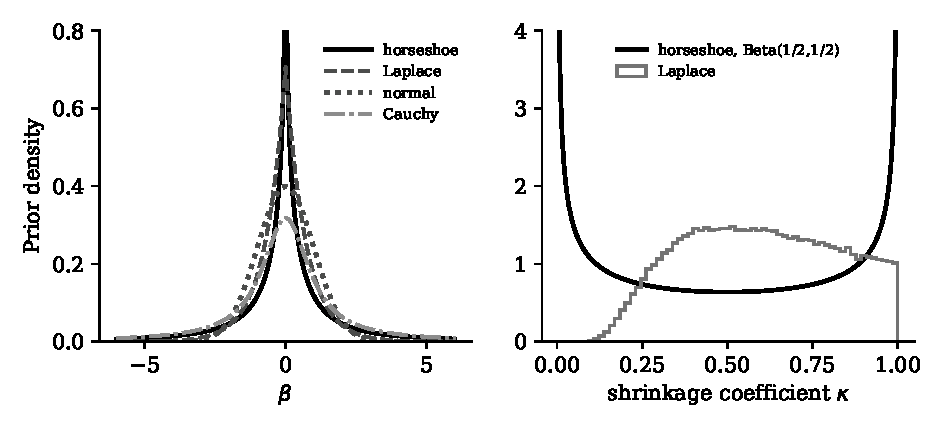
\includegraphics[width=\linewidth]{hs_prior.pdf}
\caption{Left: the horseshoe density with $\gscale = 1$, unbounded at the origin with Cauchy like tails, against a Laplace prior with unit variance, a standard normal and a standard Cauchy. Right: the implied prior on the shrinkage coefficient $\kappa$ for an observation with unit variance, the exact $\mathrm{Beta}(1/2, 1/2)$ density for the horseshoe and, for the Laplace, a histogram of $\kappa = 1/(1 + v)$ over 200,000 draws of its mixing variance $v \sim \mathrm{Exp}(1)$. The Laplace density vanishes at $\kappa = 0$, which is why the Laplace never stops shrinking large signals.}
\label{fig:hsprior}
\end{figure}
\begin{proposition}
With $\gscale = 1$, the posterior mean under the horseshoe\index{horseshoe prior!posterior mean and shrinkage profile|textbf} is
\[
\E(\beta \mid y) = y\,\{1 - \E(\kappa \mid y)\},
\]
where
\[
p(\kappa \mid y) \propto (1-\kappa)^{-1/2} e^{-\kappa y^2/2}, \qquad 0 < \kappa < 1.
\]
\end{proposition}

\begin{proof}
Given $\kappa$, $y \sim N(0, 1/\kappa)$, so the likelihood of $\kappa$ is $\kappa^{1/2}e^{-\kappa y^2/2}$. Multiply by the $\mathrm{Beta}(1/2,1/2)$ density $\kappa^{-1/2}(1-\kappa)^{-1/2}$ to obtain the stated posterior, and use $\E(\beta \mid y, \kappa) = (1-\kappa)y$.
\end{proof}

Figure~\ref{fig:profiles} compares the shrinkage profiles\index{horseshoe prior!posterior mean and shrinkage profile}, the horseshoe computed by numerical integration of the proposition. The horseshoe estimate is 0.38 at $y = 1$, shrinking noise hard; 1.06 at $y = 2$; 3.45 at $y = 4$; 5.66 at $y = 6$; and 7.75 at $y = 8$. The gap $y - \E(\beta \mid y)$ goes to zero as $y$ grows. 

\begin{figure}[ht]
\centering
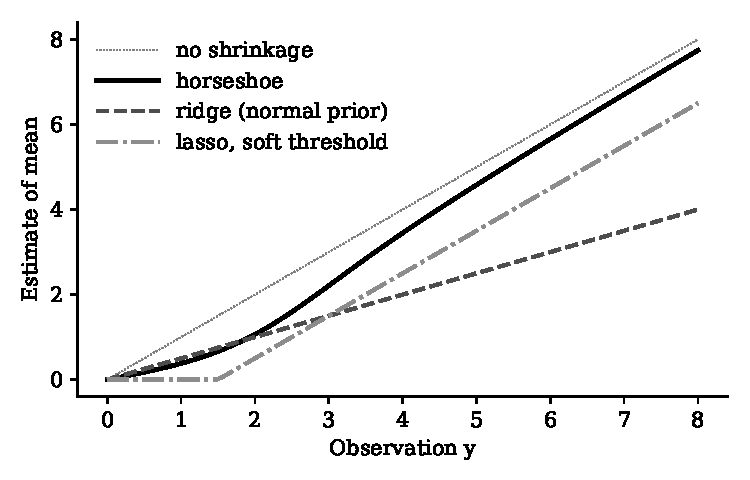
\includegraphics[width=\linewidth]{shrink_profiles.pdf}
\caption{Posterior mean as a function of the observation in the normal means problem, for the horseshoe, a normal prior with unit variance, and a lasso soft threshold at 1.5.}
\label{fig:profiles}
\end{figure}

\section{Tail robustness and regular variation}

Tweedie's formula\index{Tweedie formula@Tweedie's formula|textbf} shows why the horseshoe\index{horseshoe prior!tail robustness|textbf} leaves large signals alone\index{tail robustness|textbf}. It expresses the posterior mean through the marginal density $m(y) = \int \phi(y - \beta)\pi(\beta)\,d\beta$:
\begin{equation}
\E(\beta \mid y) = y + \frac{d}{dy}\log m(y).
\label{eq:tweedie}
\end{equation}
Shrinkage is the score of the marginal. If $m$ has light normal tails, the score grows linearly and shrinkage never stops; if $m$ has polynomial tails, the score decays and shrinkage vanishes for large $y$.

\begin{definition}[Regular variation]
A positive function $f$ on $(0,\infty)$ is regularly varying\index{regular variation|textbf} at infinity with index $\alpha$ if $f(cx)/f(x) \to c^{\alpha}$ as $x \to \infty$ for every $c > 0$.
\end{definition}

\begin{theorem}[Tail robustness]
If the prior density $\pi(\beta)$ is regularly varying at infinity with index $-\alpha$, $\alpha > 1$, and is eventually differentiable with $\beta\pi'(\beta)/\pi(\beta) \to -\alpha$, then the marginal $m(y)$ is regularly varying with the same index and
\[
y - \E(\beta \mid y) = \frac{\alpha}{y}\{1 + o(1)\} \to 0 \quad\text{as } y \to \infty.
\]
\end{theorem}

\begin{proof}[Sketch]
For large $y$, the Gaussian kernel concentrates on $\beta$ near $y$, where the prior changes little over unit distances. This gives $m(y)\sim\pi(y)$, so $m$ inherits the regular variation\index{regular variation}. The derivative hypothesis also gives $m'(y)\sim\pi'(y)$, and hence
\[
\frac{m'(y)}{m(y)}\sim\frac{\pi'(y)}{\pi(y)}\sim-\frac{\alpha}{y}.
\]
Substitution in \eqref{eq:tweedie} proves the result. Appendix~\ref{app:theory} establishes both convolution limits.
\end{proof}

The horseshoe density behaves like $\beta^{-2}$ in the tails, so $\alpha = 2$ and a large signal $y$ is shrunk by about $2/y$. At $y = 8$ that predicts about 0.25; the exact value from the proposition is 0.25. 

\section{Minimax and contraction}

Tail robustness concerns single coefficients; the global scale $\gscale$ gives adaptivity across all of them. Van der Pas, Kleijn and van der Vaart showed in 2014 that the horseshoe posterior contracts\index{posterior contraction|textbf}\index{posterior concentration|see{posterior contraction}} around a sparse truth at the minimax rate\index{minimax rate|textbf}\index{horseshoe prior!minimax rate|textbf}.

\begin{theorem}[van der Pas, Kleijn and van der Vaart]
In the normal means problem with unit variance, suppose the true mean vector has at most $s_p$ nonzero entries, with $s_p \to \infty$ and $s_p = o(p)$. If $\gscale$ is set at $(s_p/p)^{c}$ for $c \geq 1$, or estimated by an empirical Bayes\index{empirical Bayes|textbf} rule that meets the conditions of their paper, the horseshoe posterior contracts around the truth in squared $\ell_2$ distance at rate $s_p \log(p/s_p)$, the minimax rate.
\end{theorem}

A hierarchical prior on $\gscale$ supported on $[1/p,1]$, such as a truncated half Cauchy, achieves a rate of the same order without knowing $s_p$, when $\log p \lesssim s_p \le p^{a}$ for some $a < 1$, and within a logarithmic factor under weaker conditions on the hyperprior (van der Pas, Szab\'o and van der Vaart 2017a), and the horseshoe predictive density has Kullback and Leibler risk of the same minimax order. Appendix~\ref{app:guarantees} states these results, the coverage of horseshoe credible sets, and their consequences for causal functionals.  The horseshoe plus prior\index{horseshoe plus prior|textbf} of Bhadra, Datta, Polson and Willard (2017) adds a second layer of half Cauchy mixing and is aimed at ultra sparse signals.

\section{Regression and computation}\label{sec:hsregression}

In the linear regression $Y = Z\beta + \varepsilon$, $\varepsilon \sim N(0, \sigma^2 I)$, the horseshoe\index{horseshoe prior!in regression|textbf} places \eqref{eq:hs} on each coefficient, scaled by $\sigma$, so that $\beta_j \mid \lambda_j, \gscale, \sigma \sim N(0, \sigma^2\lambda_j^2\gscale^2)$, and $\sigma^2$ has the prior $p(\sigma^2) \propto 1/\sigma^2$. Makalic and Schmidt (2016) gave a simple Gibbs sampler by writing each half Cauchy as an inverse gamma mixture of inverse gammas, $\lambda_j^2 \mid \nu_j \sim \mathrm{IG}(1/2, 1/\nu_j)$ and $\nu_j \sim \mathrm{IG}(1/2, 1)$, and similarly for $\gscale^2$ with auxiliary $\xi$. All full conditionals are then standard, with $\mathrm{IG}(a, b)$ the inverse gamma of shape $a$ and rate $b$.

\begin{enumerate}
\item Draw $\beta \sim N(A^{-1}Z^\top Y, \sigma^2 A^{-1})$, where $A = Z^\top Z + \mathrm{diag}\{(\lambda_j^2\gscale^2)^{-1}\}$.
\item Draw $\sigma^2 \sim \mathrm{IG}\bigl((n + p)/2, \{\|Y - Z\beta\|^2 + \sum_j \beta_j^2/(\lambda_j^2\gscale^2)\}/2\bigr)$.
\item Draw $\lambda_j^2 \sim \mathrm{IG}\bigl(1, 1/\nu_j + \beta_j^2/(2\gscale^2\sigma^2)\bigr)$ and $\nu_j \sim \mathrm{IG}(1, 1 + 1/\lambda_j^2)$.
\item Draw $\gscale^2 \sim \mathrm{IG}\bigl((p + 1)/2, 1/\xi + \sum_j \beta_j^2/(2\lambda_j^2\sigma^2)\bigr)$ and $\xi \sim \mathrm{IG}(1, 1 + 1/\gscale^2)$.
\end{enumerate}
Coefficients that should not be shrunk, such as the treatment effect, get a flat prior by setting their prior precision to zero in $A$. They are then left out of steps 3 and 4 and of the penalty sum in step 2, and $p$ in steps 2 and 4 becomes the number of shrunk coefficients. Sections~\ref{sec:ricsim} and~\ref{sec:sharedsim} use this sampler.

Section~\ref{comp:sec:horseshoe} tests quantile networks trained on prior draws and their implied data (Polson and Sokolov 2026a) on a regression with ten coefficients. None of three pipelines was both calibrated and in agreement with the far cheaper Gibbs sampler. A network computes the posterior of its training prior; a coupled horseshoe network has not been tried.

\paragraph{Logistic outcomes with the horseshoe.}
For a binary outcome the Polya Gamma\index{Polya Gamma@P\'olya Gamma} augmentation of Chapter~\ref{ch:computation} makes horseshoe logistic regression conditionally Gaussian. With $\zeta_i = z_i^\top\beta$ and $\tilde y_i = y_i - 1/2$, draw $\omega_i \sim \mathrm{PG}(1, \zeta_i)$ and then
\[
\beta \sim N(V Z^\top\tilde y, V), \qquad V = (Z^\top\Omega Z + \Lambda^{-1})^{-1},
\]
where $\Omega = \mathrm{diag}(\omega_i)$ and $\Lambda$ is the diagonal matrix of prior variances $\lambda_j^2\gscale^2$. The scale updates are as in the Gaussian case with $\sigma^2 = 1$. The causal targets, risk differences averaged over any $Q$, follow from the draws of $\beta$ as in Chapter~\ref{ch:mccullagh}.

\paragraph{The regularized horseshoe.} Under separation, a covariate that splits the outcomes perfectly leaves the likelihood flat as its coefficient grows, so the posterior tail of that coefficient is the prior's Cauchy like tail and its posterior mean does not exist. Piironen and Vehtari (2017) cap the prior variance with a slab scale $c$,
\[
\beta_j \mid \lambda_j, \gscale, c \sim N(0, \gscale^2\tilde\lambda_j^2), \qquad \tilde\lambda_j^2 = \frac{c^2\lambda_j^2}{c^2 + \gscale^2\lambda_j^2}.
\]
For $\gscale\lambda_j$ small against $c$ this is the horseshoe; as $\lambda_j$ grows the variance approaches $c^2$, giving normal shrinkage of scale $c$ and, under separation, a Gaussian posterior tail with a finite mean. Choose $c$ on the scale of the largest plausible log odds effect of one covariate. The cap bounds the variance, not coefficients or propensities, so it does not by itself keep $\hat e$ inside $[c', 1 - c']$. The simulations of this chapter use the plain horseshoe.

\section{Why independent shrinkage confounds}

Return to the partially linear model\index{partially linear model!with linear nuisances|textbf} with linear nuisances:
\[
Y = \tau T + X^\top\beta + \varepsilon, \qquad T = X^\top\gamma + \nu.
\]
Fit the outcome regression with a shrinkage prior on $\beta$, giving the shrunk estimate $\hat\beta$, and a flat prior on $\tau$. The estimate of $\tau$ is roughly the coefficient from regressing $Y - X^\top\hat\beta$ on $T$, and
\[
\hat\tau - \tau \approx \frac{\mathrm{Cov}\{T, X^\top(\beta - \hat\beta)\}}{\mathrm{Var}(T)} = \frac{\gamma^\top \Sigma_X (\beta - \hat\beta)}{\mathrm{Var}(T)}.
\]
The bias is the shrinkage error $\beta - \hat\beta$ projected on the treatment direction $\gamma$. Confounders, with large $\gamma_j$ and large $\beta_j$, contribute most, so any prior\index{prior distribution!independent shrinkage confounds|textbf} that shrinks $\beta_j$ without regard to $\gamma_j$ shrinks confounders and biases $\tau$.

This is the regularization induced confounding\index{regularization induced confounding!remedy by coupling|textbf} of Hahn, Carvalho, Puelz and He (2018). For the lasso, subtracting a constant from every coefficient leaves a component of size $\lambda$ in $\beta - \hat\beta$ along every active confounder. 

An independent horseshoe is much better, because tail robustness makes $\beta_j - \hat\beta_j$ small for large $\beta_j$ when the confounders are not strongly correlated. But moderate confounders, with $\beta_j$ of one or two standard errors, still sit where the horseshoe shrinks substantially.

\section{The partially exchangeable horseshoe}

The proposed remedy\index{coupled prior|textbf}\index{coupled prior!horseshoe version|textbf} is to tell the prior which coefficients are confounders\index{coupling!of the outcome and treatment priors|textbf}\index{coupling}, in one of two closely related ways.

\paragraph{Shared local scales.} Place horseshoe priors on both the outcome and treatment coefficients, with a common local scale for each covariate\index{shared scale prior|textbf}\index{coupled prior!shared scale form|textbf}:
\begin{equation}
\beta_j \sim N(0, \sigma_Y^2\lambda_j^2\tau_{\mathrm{g},Y}^2), \qquad \gamma_j \sim N(0, \sigma_T^2\lambda_j^2\tau_{\mathrm{g},T}^2), \qquad \lambda_j \sim C^+(0,1).
\label{eq:shared}
\end{equation}
Here $\sigma_Y^2$ and $\sigma_T^2$ are the error variances of the outcome and treatment equations, each with prior proportional to its inverse, and the global scales $\tau_{\mathrm{g},Y}$ and $\tau_{\mathrm{g},T}$ have independent $C^+(0,1)$ priors, as in Section~\ref{sec:hsregression}. Covariates are now partially exchangeable\index{partially exchangeable horseshoe|textbf}\index{exchangeability!partial}: exchangeable within each model, linked through $\lambda_j$. A strong treatment predictor has a large posterior $\lambda_j$, protecting its outcome coefficient whether it is a confounder or a covariate that predicts treatment and not the outcome, an instrument in the language of Chapter~\ref{ch:iv}. Section~\ref{sec:sharedsim} shows that protecting instruments can cost more than it gains.

\paragraph{Propensity as a covariate.} Fit the treatment model first, obtain $\hat m(X) = X^\top\hat\gamma$, and include it in the outcome regression with a flat prior:
\[
Y = \tau T + \delta\,\hat m(X) + X^\top\beta + \varepsilon.
\]
The unshrunk $\delta$ absorbs the confounding direction $\Sigma_X\gamma$, so shrinking $\beta$ leaks much less into $\tau$. We call $\hat m(X)$ the propensity covariate: for a continuous treatment it is the fitted treatment regression, and for a binary one the estimated propensity score\index{propensity score!estimated, in the coupled prior|textbf}. This is the Bayesian causal forest\index{Bayesian causal forest} device of Hahn, Murray and Carvalho (2020), transplanted to the horseshoe.

\begin{proposition}
In vector form let $Y = \tau T + X\beta + \varepsilon$ and $T = X\gamma + \nu$, where $X$ is the $n \times p$ matrix of covariates with columns $X_j$ satisfying $\|X_j\|^2 \le Kn$, and $\nu$ is independent of $X$ with independent, mean zero, sub-Gaussian entries of variance $\sigma_\nu^2$. Suppose the treatment fit is exact, $\hat m = X\gamma \ne 0$, and let $\tilde T = T - \hat m\,(\hat m^\top T)/(\hat m^\top\hat m)$ be the residual of $T$ on $\hat m$. Put flat priors on $\tau$ and on the coefficient $\delta$ of $\hat m$, any prior on the coefficient vector $b$ of $X$, and let $\hat\beta$ be the posterior mean of $b$, however it depends on the data. Then the posterior mean of $\tau$ satisfies
\begin{equation}
\hat\tau - \tau = \frac{\tilde T^\top\varepsilon + \tilde T^\top X(\beta - \hat\beta)}{\tilde T^\top\tilde T},
\label{eq:pcbias}
\end{equation}
and, conditional on $X$, with probability tending to one as $n$ and $p$ grow, $\|X^\top\tilde T\|_\infty \le c_1\sqrt{n\log p}$ and $\tilde T^\top\tilde T \ge c_2n$, so that
\begin{equation}
\left|\frac{\tilde T^\top X(\beta - \hat\beta)}{\tilde T^\top\tilde T}\right| \le c_3\sqrt{\frac{\log p}{n}}\,\|\beta - \hat\beta\|_1,
\label{eq:pcbound}
\end{equation}
where $c_1$, $c_2$ and $c_3$ depend only on $K$, $\sigma_\nu$ and the sub-Gaussian norm of $\nu$.
\end{proposition}

\begin{proof}
Condition on $b$ and $\sigma^2$. With flat priors on $\tau$ and $\delta$, the posterior mean of $\tau$ is the least squares coefficient of $T$ when $Y - Xb$ is regressed on $T$ and $\hat m$, which by Frisch, Waugh and Lovell is $\tilde T^\top(Y - Xb)/\tilde T^\top\tilde T$. This is linear in $b$, so averaging over the posterior of $b$ replaces $b$ by $\hat\beta$; substituting $Y = \tau T + X\beta + \varepsilon$ with $\tilde T^\top T = \tilde T^\top\tilde T$ gives \eqref{eq:pcbias}.

For the bounds, write $M = I - \hat m\hat m^\top/\|\hat m\|^2$. Since $T = \hat m + \nu$ and $M\hat m = 0$, $\tilde T = M\nu$. Conditional on $X$, the $j$th coordinate of $X^\top\tilde T$ is $(MX_j)^\top\nu$, which is sub-Gaussian with scale at most $C_\nu\|MX_j\| \le C_\nu\sqrt{Kn}$, where $C_\nu$ is a constant multiple of the sub-Gaussian norm of $\nu$, so $\|X^\top\tilde T\|_\infty = O_p(\sqrt{n\log p})$ by the union bound. Next,
\[
\tilde T^\top\tilde T = \nu^\top\nu - \frac{(\hat m^\top\nu)^2}{\|\hat m\|^2} = n\sigma_\nu^2\{1 + o_p(1)\},
\]
because $\nu^\top\nu/n \to \sigma_\nu^2$ in probability and $\hat m^\top\nu/\|\hat m\|$ is sub-Gaussian with scale $C_\nu$, so the subtracted term is $O_p(1)$. The bound \eqref{eq:pcbound} follows from $|\tilde T^\top X(\beta - \hat\beta)| \le \|X^\top\tilde T\|_\infty\|\beta - \hat\beta\|_1$.
\end{proof}

Without the propensity covariate the bias term is $T^\top X(\beta - \hat\beta)/T^\top T$, and $X^\top T = X^\top X\gamma + X^\top\nu$ has coordinates of order $n$ wherever $\Sigma_X\gamma$ is not small, so the bias is of the order of the shrinkage error itself and not of $\sqrt{\log p/n}$ times its $\ell_1$ norm. The propensity covariate removes the first order term in the shrinkage error. What is left is below the sampling error, which is of order $n^{-1/2}$, when $\|\beta - \hat\beta\|_1 = o(1/\sqrt{\log p})$. That condition is of the same kind as the rate conditions of Chapter~\ref{ch:dml} and cruder than the one cross fitting gives, because the bound holds for every $\hat\beta$ however it depends on the data. The proposition concerns an exact, oracle treatment fit, and it does not say how large $\|\beta - \hat\beta\|_1$ is for the horseshoe.

 Given $\hat\beta$, the estimate solves $\sum_i\tilde T_i(Y_i - \tau T_i - X_i^\top\hat\beta) = 0$, the treatment residual times the outcome residual. At the true nuisances this is the Robinson score \eqref{eq:robscore} of Chapter~\ref{ch:dml}: with $m_0(X) = \E(T \mid X)$, $g_0(X) = X^\top\beta$ and $\ell_0 = \tau m_0 + g_0$,
\[
(T - m_0)(Y - \tau T - g_0) = (T - m_0)\{Y - \ell_0 - \tau(T - m_0)\}.
\]
Perturb the outcome fit by $h(X)$ and the score moves by $-(T - m_0)h(X)$, whose expectation is zero because $\E(T - m_0 \mid X) = 0$. This is Neyman orthogonality, reached by putting the treatment fit into the outcome model with a flat prior instead of correcting the score afterwards.

If $\hat m(X)$ misses $X^\top\gamma$, $\tilde T$ keeps a component along $X(\gamma - \hat\gamma)$, and the bias becomes the product of that error and the shrinkage error: small when either is small, and the second order term of Chapter~\ref{ch:dml}. With a binary treatment the AIPW weight $T/\hat e(X) - (1 - T)/\{1 - \hat e(X)\}$ equals the treatment residual $T - \hat e(X)$ divided by $\hat e(X)\{1 - \hat e(X)\}$, so it plays the part of $\tilde T$, and it is the clever covariate of van der Laan and Rubin (2006). Orthogonality is also why the coupled posterior and the DML estimator of Section~\ref{sec:baipw} agree when they do: both multiply the outcome residual by the treatment residual, and in both the nuisance errors enter as a product.

Appendix~\ref{app:theory} makes the product precise for a fixed coefficient vector $\hat\gamma$ in $\hat m = X\hat\gamma$ (Proposition~\ref{ss:prop:product}). Write $\Delta = \gamma - \hat\gamma$ for the error of the treatment fit, $c$ for the limit of the shrinkage error $\beta - \hat\beta$ and $\Sigma$ for the covariance of the covariates. With $p$ fixed, the bias of the posterior mean of $\tau$ tends to the covariance of $X\Delta$ and $Xc$, after the parts explained by $\hat m$ are removed, divided by the variance left in $\tilde T$. It is zero when $\Delta = 0$ and at most $\|\Sigma^{1/2}\Delta\|\,\|\Sigma^{1/2}c\|/\sigma_\nu^2$ in absolute value. The free coefficient on $\hat m$ matters: in the reduced form coordinates of Hahn, Carvalho, Puelz and He (2018) and DiTraglia and Liu (2025), where the coefficient of $T - X\hat\gamma$ is the effect, the limit has an extra term quadratic in $\Delta$. The limit says how given errors combine, not how large they are. With $p$ fixed, a posterior mean that is consistent for $b + \delta\hat\gamma$, the coefficient vector of $X$ that the data identify, makes it zero, so a nonzero limit needs a prior that excludes the true coefficients or a $p$ that grows with $n$. Section~\ref{sec:baipw} takes up the rates, and for the horseshoe logistic propensity model we cannot supply them.



\paragraph{Back to Robins and Ritov.}
The coupled prior of Section~\ref{sec:rrw} centres each cell's outcome probability on a function of its selection probability. Here the outcome coefficient's scale is tied to its treatment coefficient. Both priors encode a relation between selection and outcome; there, it turns an inconsistent posterior into a consistent one.

Orthogonalization and cross fitting\index{cross fitting} protect the target from nuisance shrinkage by construction of the estimator; the coupled horseshoe\index{coupled horseshoe|see{coupled prior}} attacks the same leak by construction of the prior, and keeps the posterior, with every other causal summary.

\section{A first test of coupling}\label{sec:ricsim}

The test\index{coupled prior!first test of|textbf} is a simulation\index{simulation study!coupling, first test|textbf} in the partially linear model $Y = \tau T + X^\top\beta + \varepsilon$, $T = X^\top\gamma + \nu$, with $n = 200$ observations and $p = 50$ independent standard normal covariates. Five are confounders with $\gamma_j = \beta_j = 1$ and the other 45 have zero coefficients in both equations; $\nu$ and $\varepsilon$ are independent standard normal, there is no intercept, and $\tau = 1$. Over 500 data sets we report each estimator's bias, root mean squared error (RMSE) and the coverage\index{coverage!simulated|textbf} of its nominal 95 percent interval.

Seven estimators are compared. Least squares on $T$ and all 50 covariates needs no regularization, and least squares on $T$ and the five true confounders is an oracle that no analyst can compute. The lasso plug in is the coefficient of $T$ in a lasso of $Y$ on $T$ and the covariates. DML is the partialling out estimator of Chapter~\ref{ch:dml} with five fold cross fitting, lasso fits of $Y$ and of $T$ on $X$, and a sandwich interval. The independent horseshoe puts the prior \eqref{eq:hs} on the 50 covariate coefficients and a flat prior on $\tau$. The coupled horseshoe adds the lasso fit $\hat m(X)$ of the treatment to that regression as a covariate with a flat prior, either fitted once on the whole sample (the row labelled $\hat m(X)$) or cross fitted on the five folds that DML uses (the row labelled cross fitted). Every lasso penalty is chosen by five fold cross validation, and every horseshoe is a Gibbs run of 1,500 sweeps with the first 500 discarded, reporting the posterior mean and the central 95 percent posterior interval. In 20 data sets of this design, four chains from the default start gave a split $\hat R$ for the coefficient of $T$ of at most 1.003 (independent prior) and 1.007 (coupled prior), with at least 1,340 effective draws out of 4,000 (Section~\ref{comp:sec:cost}).

\begin{table}[ht]
\centering
\small
\caption{Bias, root mean squared error (RMSE) and coverage of seven estimators of $\tau = 1$ over 500 simulated data sets with $n = 200$ and $p = 50$. Coverage is for nominal 95\% intervals: the classical $t$ interval for least squares, the sandwich interval for DML and the central 95\% posterior interval for each horseshoe. The lasso plug in has no interval. The oracle regression uses the five true confounders only and is not available in practice. Monte Carlo standard errors are at most 0.004 for the biases, 0.004 for the RMSEs and 0.019 for the coverages.}
\label{tab:ric}
\begin{tabular}{@{}>{\raggedright\arraybackslash}p{2.3in}ccc@{}}
\toprule
Estimator & Bias & RMSE & Coverage \\
\midrule
Least squares, all covariates & $-$0.002 & 0.084 & 0.944 \\
Least squares, five true confounders (oracle) & $-$0.002 & 0.076 & 0.934 \\
Lasso plug in & 0.212 & 0.230 &  \\
DML, lasso nuisances & 0.009 & 0.079 & 0.924 \\
Horseshoe, independent prior & 0.059 & 0.103 & 0.868 \\
Horseshoe, coupled to $\hat m(X)$ & $-$0.023 & 0.084 & 0.918 \\
Horseshoe, coupled to cross fitted $\hat m(X)$ & 0.088 & 0.114 & 0.764 \\
\bottomrule
\end{tabular}
\end{table}


\begin{figure}[ht]
\centering
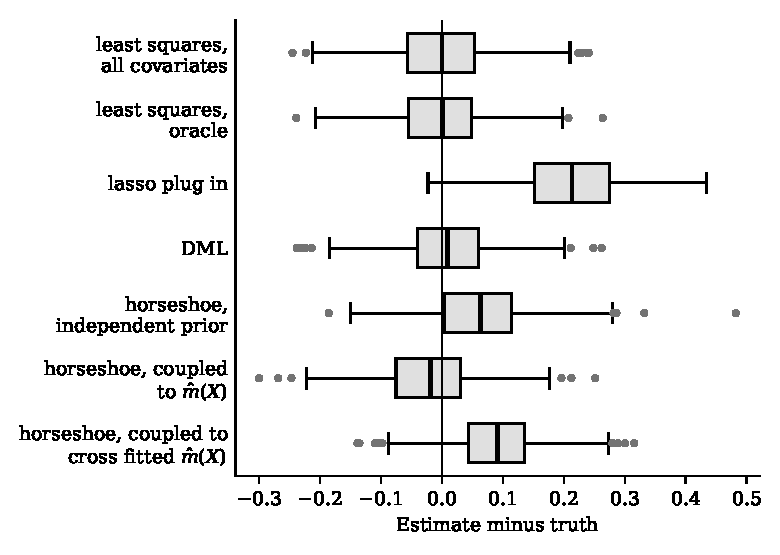
\includegraphics[width=\linewidth]{ric.pdf}
\caption{Estimate minus the truth for seven estimators of $\tau = 1$ over 500 simulated data sets with $n = 200$ and $p = 50$. Boxes span the quartiles, the heavy line is the median, whiskers reach the most extreme estimate within 1.5 interquartile ranges of the box, and dots are estimates beyond that.}
\label{fig:ric}
\end{figure}

In Table~\ref{tab:ric} and Figure~\ref{fig:ric}, least squares on all the covariates is unbiased, covers 0.944 and has the same RMSE as the coupled horseshoe, 0.084, and DML, at 0.079, is slightly better than both. The design therefore tests regularization induced confounding and does not show a gain over a method that does no regularization. 

The lasso plug in is biased by 0.212, a fifth of the effect. DML removes most of that (0.009), and the independent horseshoe keeps some (0.059) and covers 0.868. Coupling to the whole sample $\hat m(X)$ takes the bias from 0.059 to $-0.023$, the RMSE from 0.103 to 0.084 and the coverage from 0.868 to 0.918, and the coupled posterior is closer to the truth than the independent one in 58 percent of the data sets. It is slightly less accurate than DML, which is closer to the truth in 54 percent. The Monte Carlo standard errors are at most 0.004 for biases and RMSEs and 0.019 for coverages, so 500 data sets separate DML and the coupled posterior from the plug in and the independent horseshoe, and only just separate them from each other (a paired $t$ of 2.8 on the squared errors). Their coverages, 0.924 and 0.918, cannot be ranked, and both fall short of 0.95 by more than two standard errors.

Cross fitting the propensity covariate makes coupling worse. The cross fitted version has bias 0.088, RMSE 0.114 and coverage 0.764, and it is closer to the truth than the whole sample version in only 32 percent of the data sets. 

Least squares matched the coupled posterior because $p$ is small against $n$. We therefore repeated the simulation with $p = 150$ and $p = 300$, keeping $n = 200$, the five confounders, the 500 data sets and every other detail of the design (Tables~\ref{tab:ric_hd150} and~\ref{tab:ric_hd300}). With $p = 150$ least squares is still defined, with 49 residual degrees of freedom, and with $p = 300$ it does not exist. The oracle regression is unaffected, with RMSE 0.069 and 0.071.

\begin{table}[ht]
\centering
\small
\caption{Bias, root mean squared error (RMSE) and coverage of seven estimators of $\tau = 1$ over 500 simulated data sets with $n = 200$ and $p = 150$. Coverage is for nominal 95\% intervals: the classical $t$ interval for least squares, the sandwich interval for DML and the central 95\% posterior interval for each horseshoe. The lasso plug in has no interval. The oracle regression uses the five true confounders only and is not available in practice. The least squares interval uses $n - p - 1 = 49$ degrees of freedom. Monte Carlo standard errors are at most 0.006 for the biases, 0.007 for the RMSEs and 0.021 for the coverages.}
\label{tab:ric_hd150}
\begin{tabular}{@{}>{\raggedright\arraybackslash}p{2.3in}ccc@{}}
\toprule
Estimator & Bias & RMSE & Coverage \\
\midrule
Least squares, all covariates & 0.008 & 0.138 & 0.960 \\
Least squares, five true confounders (oracle) & 0.005 & 0.069 & 0.946 \\
Lasso plug in & 0.370 & 0.386 &  \\
DML, lasso nuisances & 0.026 & 0.080 & 0.902 \\
Horseshoe, independent prior & 0.067 & 0.107 & 0.838 \\
Horseshoe, coupled to $\hat m(X)$ & $-$0.045 & 0.096 & 0.912 \\
Horseshoe, coupled to cross fitted $\hat m(X)$ & 0.113 & 0.134 & 0.654 \\
\bottomrule
\end{tabular}
\end{table}


\begin{table}[ht]
\centering
\small
\caption{Bias, root mean squared error (RMSE) and coverage of seven estimators of $\tau = 1$ over 500 simulated data sets with $n = 200$ and $p = 300$. Coverage is for nominal 95\% intervals: the classical $t$ interval for least squares, the sandwich interval for DML and the central 95\% posterior interval for each horseshoe. The lasso plug in has no interval. The oracle regression uses the five true confounders only and is not available in practice. Least squares on all the covariates needs $n - p - 1 > 0$ degrees of freedom and is not defined here ($n - p - 1 = -101$), so its row reads n/a. Monte Carlo standard errors are at most 0.007 for the biases, 0.008 for the RMSEs and 0.022 for the coverages.}
\label{tab:ric_hd300}
\begin{tabular}{@{}>{\raggedright\arraybackslash}p{2.3in}ccc@{}}
\toprule
Estimator & Bias & RMSE & Coverage \\
\midrule
Least squares, all covariates & n/a & n/a & n/a \\
Least squares, five true confounders (oracle) & 0.005 & 0.071 & 0.956 \\
Lasso plug in & 0.516 & 0.543 &  \\
DML, lasso nuisances & 0.031 & 0.084 & 0.892 \\
Horseshoe, independent prior & 0.067 & 0.111 & 0.856 \\
Horseshoe, coupled to $\hat m(X)$ & $-$0.071 & 0.124 & 0.836 \\
Horseshoe, coupled to cross fitted $\hat m(X)$ & 0.128 & 0.148 & 0.562 \\
\bottomrule
\end{tabular}
\end{table}


DML is the most accurate estimator an analyst can compute in both designs, and its RMSE barely moves, 0.079, 0.080 and 0.084 at $p = 50$, 150 and 300. The coupled horseshoe loses more: its RMSE is 0.084, 0.096 and 0.124, and its bias goes from $-0.023$ to $-0.045$ and $-0.071$, against $+0.059$, $+0.067$ and $+0.067$ for the independent horseshoe. Replication by replication, the squared error of the coupled posterior exceeds that of DML by an amount with a paired $t$ of 2.8, 4.2 and 7.2 at the three values of $p$, and the coupled posterior is the closer one in 46, 45 and 42 percent of the data sets. Least squares on all the covariates has RMSE 0.138 at $p = 150$, 1.7 times that of DML.

The gain of coupling over the independent horseshoe does not survive the larger designs with five confounders. Its RMSE was 0.019 smaller at $p = 50$ (paired $t = -4.8$), is 0.011 smaller at $p = 150$ ($t = -1.4$) and is 0.013 larger at $p = 300$ ($t = 1.5$), and the last two cannot be told from zero with 500 data sets. The sign of the coupled posterior's bias is opposite to that of the independent horseshoe in all three designs and its size grows with $p$. The decomposition below places it in the residual of $T$ on $\hat m(X)$, which is slightly negatively correlated with $X\gamma$, more so as $p$ grows; why it is negatively correlated we have not found.

Apart from least squares at $p = 150$, whose intervals are twice as long as DML's (median length 0.569 against 0.268) and cover 0.960, no estimator that an analyst can compute covers at the nominal rate in the larger designs. At $p = 150$ the coupled posterior covers 0.912 and DML 0.902; at $p = 300$ they cover 0.836 and 0.892. A coverage here has a Monte Carlo standard error of at most 0.022, so 0.836 is about seven standard errors below 0.95, and 15 percent of the coupled posterior's intervals lie wholly below the truth, in line with its negative bias. The cross fitted version covers 0.654 and 0.562 and is less accurate than the independent horseshoe as well.

The five confounders of these designs are strong, with unit coefficients. To see what happens when confounding is spread thin, we ran one more design with $n = 200$ and $p = 150$ standard normal covariates. The first 30 are confounders with $\gamma_j = \beta_j = 0.3$, the next four affect only the outcome, with $\beta_j = 1$ and $\gamma_j = 0$, and the other 116 have zero coefficients in both equations; $\nu$ and $\varepsilon$ are independent standard normal, there is no intercept, and $\tau = 1$. The seven estimators, the penalties, the sampler, the folds and the random seeds are those of the designs above, except that the oracle regression now uses $T$ and the 30 confounders and so leaves the four outcome only covariates in its error. Table~\ref{tab:ric_weak30} reports bias, RMSE and coverage over 500 data sets. The shared seeds give the same covariates and errors as the five confounder design at $p = 150$, so least squares repeats its row in Table~\ref{tab:ric_hd150}.

\begin{table}[ht]
\centering
\small
\caption{Bias, root mean squared error (RMSE) and coverage of seven estimators of $\tau = 1$ over 500 simulated data sets with $n = 200$ and $p = 150$, 30 confounders with $\gamma_j = \beta_j = 0.3$ and four outcome only covariates with $\beta_j = 1$. Coverage is for nominal 95\% intervals: the classical $t$ interval for least squares, the sandwich interval for DML and the central 95\% posterior interval for each horseshoe. The lasso plug in has no interval. The oracle regression uses the 30 confounders only, so the four outcome only covariates stay in its error, and it is not available in practice. The least squares interval uses $n - p - 1 = 49$ degrees of freedom. Monte Carlo standard errors are at most 0.008 for the biases, 0.006 for the RMSEs and 0.019 for the coverages.}
\label{tab:ric_weak30}
\begin{tabular}{@{}>{\raggedright\arraybackslash}p{2.3in}ccc@{}}
\toprule
Estimator & Bias & RMSE & Coverage \\
\midrule
Least squares, all covariates & 0.008 & 0.138 & 0.960 \\
Least squares, 30 true confounders (oracle) & 0.002 & 0.168 & 0.954 \\
Lasso plug in & 0.615 & 0.620 &  \\
DML, lasso nuisances & 0.069 & 0.126 & 0.756 \\
Horseshoe, independent prior & 0.670 & 0.672 & 0.000 \\
Horseshoe, coupled to $\hat m(X)$ & 0.004 & 0.113 & 0.944 \\
Horseshoe, coupled to cross fitted $\hat m(X)$ & 0.467 & 0.471 & 0.000 \\
\bottomrule
\end{tabular}
\end{table}


The ranking of the strong designs is reversed. The lasso plug in is biased by 0.615 and the independent horseshoe by 0.670, about two thirds of the effect, and no interval of the independent horseshoe covers the truth: with thirty coefficients of 0.3 both shrink the confounders hard. DML removes most of that bias but not all of it. Its bias is 0.069, its intervals are short (median length 0.284), and they cover 0.756, with 22 percent lying wholly above the truth. The coupled horseshoe with the whole sample $\hat m(X)$ has bias 0.004, RMSE 0.113 and coverage 0.944, within a Monte Carlo standard error of 0.95, with a median interval length of 0.410. It is the most accurate estimator in the table and is closer to the truth than DML in 57 percent of the data sets; its squared error is below DML's by 0.0032 on average, with a paired standard error of 0.0012. Least squares on all the covariates covers 0.960, but its RMSE of 0.138 exceeds the coupled posterior's by an amount with a paired $t$ of 5.0. The oracle is less accurate than both (RMSE 0.168), because the four outcome only covariates it leaves out raise its error variance from one to five.

Cross fitting the propensity covariate fails badly here. The cross fitted version has bias 0.467 and RMSE 0.471, none of its 500 intervals covers the truth, and it is closer to the truth than the whole sample version in one data set of the 500. Its bias is about four times that with five strong confounders at $p = 150$ (0.113), and about 70 percent of the independent horseshoe's 0.670.

Equation~\eqref{eq:pcbias} separates the error of either coupled fit into two terms, with $\tilde T$ the residual of $T$ on that fit's $\hat m$ and $\hat\beta$ the posterior mean of its covariate coefficients. The first, in $\varepsilon$, has mean zero conditional on $T$ and $X$, because $\hat m$ is fitted using only $T$ and $X$ and $\varepsilon$ is independent of both. The expected second term is therefore the bias: shrinkage error weighted by the covariate variation left in the treatment residual.

Proposition~\ref{ss:prop:product} gives the product formula for fixed $p$ and fixed $\hat\gamma$ in $\hat m=X\hat\gamma$. It does not explain the difference between our coupled fits, so we measured it. We reran the four designs with the seeds of the tables and computed, in each of the 500 data sets and for both coupled fits, the two terms of \eqref{eq:pcbias}, the correlation of $\tilde T$ with the confounding signal $X\gamma$, and the $\ell_1$ norm of the shrinkage error $\beta - \hat\beta$. With thirty weak confounders the second term carries the bias. Averaged over the data sets it is 0.465 for the cross fitted version, whose bias is 0.467, and $-0.001$ for the whole sample version, with a Monte Carlo standard error of 0.003; the first term averages 0.005 or less in both. The shrinkage error is not what differs. Over the 30 confounders its $\ell_1$ norm averages 8.54 for the whole sample fit and 8.42 cross fitted, both close to the 9 it would be if every confounder's coefficient were estimated as zero. What differs is $\tilde T$: its correlation with $X\gamma$ averages 0.420 when $\hat m$ is cross fitted and 0.007 when it is fitted on the whole sample. The cross fitted residual keeps part of the confounding signal, and the second term passes the shrinkage error through it into $\tau$. The designs with five strong confounders repeat the pattern on a smaller scale. Cross fitted, the second term averages 0.089, 0.108 and 0.123 at $p = 50$, 150 and 300, against biases of 0.088, 0.113 and 0.128, with correlations of 0.041 to 0.060. Whole sample, it averages $-0.021$, $-0.052$ and $-0.077$, close to the coupled posterior's biases of $-0.023$, $-0.045$ and $-0.071$, with correlations of $-0.010$ to $-0.028$. These are measured averages over four designs, not a theorem. We have not found why the residual on the whole sample lasso fit carries almost none of $X\gamma$ when the same lasso, fitted on four fifths of the data and evaluated on the rest, leaves a correlation of 0.420. Nor have we separated two possible causes of the failure: a different lasso fit in each fold, so that $\hat m$ is not one linear function of the columns of $X$, and fitting on four fifths of the sample.

With five strong confounders, then, the coupled horseshoe is not a substitute for DML when $p$ is large, and its gain over the independent horseshoe at $p = 50$ is not resolved at $p = 150$ or $p = 300$, although at $p = 150$ the coupled intervals cover more often (0.912 against 0.838). With thirty weak confounders the coupled posterior is the most accurate estimator, and apart from least squares the only one an analyst can compute whose intervals cover at the nominal rate. We ran one value of $n$, two patterns of confounding, independent covariates, a lasso nuisance learner and one sampler setting. Denser confounding, correlated covariates, other nuisance learners, repeated cross fitting and other ratios of $p$ to $n$ are not tested; the sampler's convergence was checked only for the coefficient of $T$, in 20 data sets at $p = 50$, 10 each at $p = 150$ and 300 with five confounders, and 10 with thirty weak confounders, where both coupled priors passed and the independent horseshoe mixed more slowly, with $\hat R$ up to 1.020 and as few as 234 effective draws out of 4,000 (Section~\ref{comp:sec:cost}).

The practical consequence is narrow. If the horseshoe is coupled, fit the propensity covariate once on the whole sample, or use a known one as in the proposition above, and do not cross fit it; coupling then needs no sample splitting. Both families of designs have no instruments and a linear treatment model, and an analyst does not know in advance which family a problem belongs to. Chapter~\ref{ch:critique} finds the same kind of result in five other designs with $n = 300$ and $p = 400$: the Bayesian reduced form leaves a positive bias in all five, and in the sparse designs with good overlap DML with a cross validated lasso has the smaller bias (Section~\ref{sec:crit:bayes}).

\section{Shared scales and instruments: a simulation}\label{sec:sharedsim}

We tested the shared scale prior\index{shared scale prior}\index{coupled prior!shared scale form} \eqref{eq:shared} against independent horseshoe\index{horseshoe prior} priors with three kinds of covariate\index{simulation study!shared scales and instruments|textbf}. Of $p = 50$ standard normal covariates, five are moderate confounders with $\beta_j = \gamma_j = 0.5$; five are instruments, with $\gamma_j = 1$ and no outcome effect; five are prognostic, with $\beta_j = 1$ and $\gamma_j = 0$; the rest are noise. Treatment is $T = X^\top\gamma + \nu$ and the outcome $Y = T + X^\top\beta + \varepsilon$, with $n = 200$ and $\nu$ and $\varepsilon$ independent standard normal. Both priors were fitted by joint Gibbs sampling of the treatment and outcome models, 1,500 sweeps per fit with the first 500 discarded, over 40 replications.

\begin{figure}[ht]
\centering
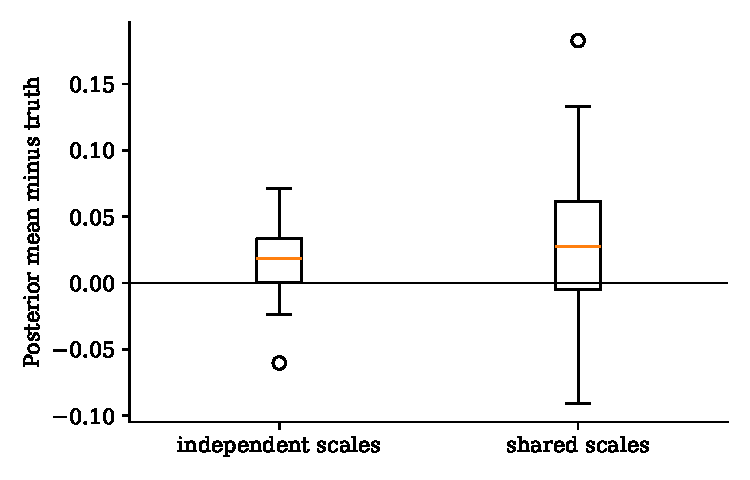
\includegraphics[width=\linewidth]{shared.pdf}
\caption{Posterior mean of $\tau$ minus the truth under independent and shared local scales, 40 replications with moderate confounders, instruments and prognostic covariates.}
\label{fig:shared}
\end{figure}

Figure~\ref{fig:shared} and the table below summarize the result.

\begin{center}
\begin{tabular}{lccc}
\toprule
Prior & Bias & RMSE & 95\% coverage \\
\midrule
Independent scales & 0.017 & 0.031 & 40 of 40 \\
Shared scales & 0.036 & 0.067 & 38 of 40 \\
\bottomrule
\end{tabular}
\end{center}


The result runs against the intuition behind the shared prior. Sharing scales protected the moderate confounders, but also the five instruments, whose large treatment coefficients left their zero outcome coefficients barely shrunk. Unshrunk instruments in an outcome regression inflate variance and, with residual confounding, amplify bias, the bias amplification\index{bias amplification|textbf} of Pearl (2011) and Wooldridge (2016). Here that cost outweighed the protection of confounders.

The independent horseshoe did well, and the instruments explain most of it. The bias of a shrunken estimate is the shrinkage error on the confounders' coefficients, projected on $\gamma$ and divided by $\mathrm{Var}(T)$, and the instruments raise $\mathrm{Var}(T)$ from 2.25 to 7.25. Exercise~\ref{ex:ch07:7} runs the design without them, where the independent prior has bias 0.074 and the shared prior 0.046, and the ratio $2.25/7.25$ turns 0.074 into a predicted 0.023 for the independent prior here, against 0.017 in the 40 replications of the table and 0.021 in 100.

The coupled prior should protect an outcome coefficient in proportion to the covariate's role as a confounder, which needs both $\gamma_j$ and $\beta_j$ nonzero; a shared scale can protect on the evidence of $\gamma_j$ alone. One refinement adds a private local scale to the shared one, $\beta_j \sim N(0, \sigma_Y^2\lambda_j^2\eta_j^2\tau_{\mathrm{g},Y}^2)$ with $\lambda_j$ shared and $\eta_j$ private. Problem~9 of Chapter~\ref{ch:open} compares independent scales, shared scales, this product prior\index{product prior|textbf}\index{coupled prior!product form|textbf} and the propensity covariate in this design. Independent scales did best, for the reason given above. The product prior recovers most of what sharing loses but still lets instruments through, and the propensity covariate is the least biased of the four but imports the variance of the instruments that dominate $\hat\gamma$. 

\section{Choosing the global scale}

The global scale\index{global scale!choice of|textbf} $\gscale$ controls how many coefficients escape shrinkage; under the continuous horseshoe none is exactly zero. With orthogonal columns of squared norm $n$ and the prior variance $\sigma^2\lambda_j^2\gscale^2$ of Section~\ref{sec:hsregression}, Piironen and Vehtari (2017) define the effective number\index{effective number of nonzero coefficients|textbf} of nonzero coefficients,
\[
\kappa_j = \frac{1}{1 + n\lambda_j^2\gscale^2}, \qquad m_{\mathrm{eff}} = \sum_{j=1}^p (1 - \kappa_j),
\]
and show that under half Cauchy local scales
\[
\E(m_{\mathrm{eff}} \mid \gscale) = \frac{p\sqrt{n}\,\gscale}{1 + \sqrt{n}\,\gscale}.
\]
They recommend scaling the prior\index{horseshoe prior!choice of global scale|textbf} on $\gscale$ by the value at which this mean equals a guess $p_0$ of the number of relevant covariates,
\[
\tau_{\mathrm{g},0} = \frac{p_0}{p - p_0}\,\frac{1}{\sqrt{n}}.
\]
Their coefficient prior is not scaled by $\sigma$, so their version of the formula carries a factor $\sigma$ that ours absorbs, and with correlated columns $m_{\mathrm{eff}}$ is an approximation. In causal problems $p_0$ is the analyst's guess at the number of confounders and prognostic variables. With $p = 50$ and a guess of $p_0 = 10$ relevant covariates, as in Section~\ref{sec:sharedsim}, the coefficient's prior scale $\sigma\tau_{\mathrm{g},0}$ is a quarter of $\sigma/\sqrt{n}$, the scale of a single noise coefficient.

The half Cauchy prior on $\gscale$ in \eqref{eq:hs} is a good default for moderate $p$. With thousands of covariates and only a handful relevant, a more concentrated prior can keep small coefficients from pulling $\gscale$ upward. Report the posterior of $m_{\mathrm{eff}}$ with the treatment effect; a large departure from $p_0$ suggests revisiting the sparsity guess or the model.

\paragraph{Effective number of confounders.}
A useful causal diagnostic is the posterior of the effective number of protected confounders,
\[
c_{\mathrm{eff}} = \sum_{j=1}^p (1 - \kappa_j^{Y})(1 - \kappa_j^{T}),
\]
where $\kappa_j^Y$ and $\kappa_j^T$ are the shrinkage coefficients of covariate $j$ in the outcome and treatment models. A covariate contributes only if it escapes shrinkage in both. With independent covariates, a $c_{\mathrm{eff}}$ concentrated near zero suggests little measured confounding. With correlated covariates it does not: a covariate that drives treatment and a correlated one that drives the outcome confound the effect while each escapes shrinkage in one model only, so $c_{\mathrm{eff}}$ is read beside the change from the unadjusted estimate and not in place of it. If it is large, adjustment matters, and the analyst should check that the confounder model is flexible enough. In the design of Section~\ref{sec:sharedsim}, with five confounders, five instruments and five prognostic covariates, only the confounders should add to $c_{\mathrm{eff}}$, since the instruments escape shrinkage only in the treatment model and the prognostic covariates only in the outcome model. With shared scales the five instruments, whose outcome coefficients were barely shrunk, would be counted as well.



\section{Horseshoe versus spike and slab}

The spike and slab\index{spike and slab prior|textbf} prior places a point mass at zero and a diffuse slab elsewhere:
\[
\beta_j \sim (1 - w)\delta_0 + w\,N(0, v).
\]
Its strength is variable selection\index{variable selection|textbf}: posterior inclusion probabilities\index{posterior inclusion probability|textbf} have a direct interpretation, and large coefficients are nearly unshrunk. Its drawback is computational. The posterior mixes over $2^p$ models, and stochastic search mixes slowly when covariates are correlated, exactly the causal situation where confounders predict treatment.

The horseshoe\index{horseshoe prior!versus spike and slab|textbf} is a continuous relaxation. The $\mathrm{Beta}(1/2, 1/2)$ prior on $\kappa_j$ puts most mass near zero and one, mimicking the discrete choice, while the continuous posterior is easy for Gibbs sampling. Carvalho, Polson and Scott (2010) showed that horseshoe posterior means closely track spike and slab posterior means in sparse problems, at a fraction of the cost.

Under the spike and slab, $1 - \kappa_j$ is replaced by the posterior inclusion probability times the slab shrinkage factor $v/(1 + v)$; under the horseshoe, $1 - \E(\kappa_j \mid y)$ plays the role of a soft inclusion probability\index{inclusion probability}, and $m_{\mathrm{eff}}$ and $c_{\mathrm{eff}}$ are its versions of the expected model size and the expected number of confounders. The practical case for the horseshoe is that it runs inside a Gibbs sampler with the treatment model, the propensity covariate and the Polya Gamma augmentation, so that every coupling of this chapter is a change of a few lines; a spike and slab with the same couplings would need a model search over the treatment and outcome models jointly. Where $p$ is small and inclusion probabilities are themselves the object of interest, the spike and slab remains the better tool.

\section{Nonlinear nuisances}

Real nuisances\index{nuisance function!nonlinear, under the horseshoe|textbf} are rarely linear; two extensions keep the horseshoe central.

The first is a basis expansion, $g(x) = \sum_k \beta_k b_k(x)$ for splines, wavelets, or random features, with the horseshoe on $\beta_k$. Tail robustness protects the large coefficients that carry the sharp features of $g$, and shared local scales with the propensity expansion protect the basis directions that predict treatment, instruments among them. The design matrix $Z$ of the Gibbs sampler now holds basis evaluations, and sparsity now means sparsity in the basis. On a spline or wavelet basis a smooth nuisance has a few large coefficients on the coarse functions and many small ones on the fine, the pattern the horseshoe is built for; a signal spread over many small coefficients defeats any sparsity prior, as the dense outcome of Design II in Section~\ref{sec:baipw} shows for raw covariates.

The second puts a horseshoe on a neural network's final layer or all its weights. GenTE (Chapter~\ref{ch:gente}) passes a learned propensity embedding to the baseline network but not the effect network, the neural analogue of the propensity covariate. Both extensions protect directions that predict treatment by giving the outcome model the estimated propensity or shared scales. The choice between a basis and a network depends on the dimension of $x$ and the expected smoothness of $g$.

\section{A horseshoe inside double machine learning}\chlabel{ch:baipw}\label{sec:baipw}

A reader who wants DML's frequentist guarantee anyway can keep it and still ask where a Bayesian model belongs. Nareklishvili, Polson and Sokolov (2026a) answer: inside DML, as the nuisance estimator\index{Bayesian AIPW!inside double machine learning|textbf}. DML supplies Neyman orthogonality and cross fitting, and the horseshoe supplies the fits of the outcome and treatment regressions.



\subsection{Where the two approaches meet}

DML is agnostic about how the nuisances are estimated. Any learner can be plugged in whose errors satisfy a product rate condition,
\[
\|\hat\mu_t - \mu_t\|\,\|\hat e - e\| = o_p(n^{-1/2}),
\]
with $\mu_t$ the outcome regression in arm $t$ and $e$ the propensity score. If the nuisances converge fast enough the estimator is root $n$ normal with valid standard errors, and if they do not, careful cross fitting cannot save it. 

A horseshoe prior offers three things to such a fit. Tail robustness leaves large confounder coefficients unshrunk, the global scale shrinks the many small ones hard, and in the propensity logit shrinkage toward the intercept tempers the inverse weights that destabilize augmented estimators. Whether the fitted nuisances meet the product rate is a separate question.

\paragraph{What the horseshoe does to the weights.} Cross validation tunes the lasso propensity to predict treatment, which need not stabilize $1/\hat e$. The horseshoe shrinks logit coefficients unless the data insist; its heavy tails can leave large coefficients and extreme propensities alone. The posterior mean of $\expit(\gamma^\top x)$ lies in $(0,1)$, but overlap $c \leq e \leq 1 - c$ does not put finite sample estimates in $[c, 1 - c]$. Uniform consistency puts them in $[c - \epsilon, 1 - c + \epsilon]$ with probability tending to one for every $\epsilon > 0$. Design I shows the tempering, and Design III its absence.

\subsection{The estimator}

We ran the idea in two forms. The first is the partialling out score of Robinson (1988) for the partially linear model $Y = \tau T + g(X) + \varepsilon$ with a binary treatment, and it is the form behind the 500 replication grid below. Write $m(x) = \E(T \mid X = x)$, which is the propensity score, and $\ell(x) = \E(Y \mid X = x)$. In each of five cross fitting folds a horseshoe linear regression of $Y$ on $X$ gives $\hat\ell$ and a horseshoe logistic regression of $T$ on $X$ gives $\hat m$, both fitted on the other four folds by the Gibbs samplers of Section~\ref{sec:hsregression}, the logistic one through Polya Gamma augmentation, each for 600 sweeps with the first 200 discarded. The fitted propensity is the logistic function at the posterior mean coefficients, clipped to $[0.01, 0.99]$. With $\tilde Y_i = Y_i - \hat\ell(X_i)$ and $\hat V_i = T_i - \hat m(X_i)$ evaluated on the held out fold,
\[
\begin{gathered}
\hat\tau = \frac{\sum_i\hat V_i\tilde Y_i}{\sum_i\hat V_i^2},
\qquad
\widehat{\mathrm{se}} = \frac{\{n^{-1}\sum_i\hat\psi_i^2\}^{1/2}}{\hat J\sqrt n}, \\
\hat\psi_i = \hat V_i(\tilde Y_i - \hat\tau\hat V_i),
\qquad
\hat J = n^{-1}\sum_i\hat V_i^2.
\end{gathered}
\]
Since $\ell = \tau m + g$ inherits the shape of $m$, a linear $\hat\ell$ is misspecified whenever the propensity is nonlinear in the covariates.

The second form is the augmented inverse probability weighted (AIPW) score, which is what our own check below runs. Within each fold, separate horseshoe linear regressions on the treated and the control units of the other folds give $\hat\mu_1$ and $\hat\mu_0$, and a horseshoe logistic regression gives $\hat e$ as the posterior mean of $\expit(\gamma^\top x)$ over the draws. The score is
\[
\begin{gathered}
\hat\psi_i = \hat\mu_1(X_i) - \hat\mu_0(X_i) + h_i\bigl\{Y_i - \hat\mu_{T_i}(X_i)\bigr\}, \\
h_i = \frac{T_i}{\hat e(X_i)} - \frac{1 - T_i}{1 - \hat e(X_i)},
\end{gathered}
\]
the estimate is $\hat\tau_B = n^{-1}\sum_i\hat\psi_i$, and its variance estimate is $n^{-2}\sum_i(\hat\psi_i - \hat\tau_B)^2$. We call this form Bayesian AIPW\index{Bayesian AIPW|textbf}, since every nuisance in it is a posterior mean.

Double robustness is due to Robins, Rotnitzky and Zhao (1994); cross fitted normality is Theorem 5.1 of Chernozhukov et al. (2018).

\begin{theorem}[Double robustness and normality]
Suppose $c \leq e_0 \leq 1 - c$ for some $c > 0$, and that with probability tending to one every fitted propensity lies in $[c', 1 - c']$ for some fixed $c' > 0$. If either $\hat e$ or $\hat\mu_t$ is consistent and the other converges to some limit, $\hat\tau_B$ is consistent. If both are consistent, at rates $r_n$ and $s_n$ with $r_ns_n = o_p(n^{-1/2})$, then under moment conditions $\sqrt{n}(\hat\tau_B - \tau_0)$ converges in distribution to $N(0, V_0)$ with $V_0$ the semiparametric efficiency bound, and $n$ times the plug in variance estimate converges in probability to $V_0$.
\end{theorem}

The rates are the assumption, and for the horseshoe we cannot supply them. Known contraction results cover normal means (van der Pas, Kleijn and van der Vaart 2014; van der Pas, Szab\'o and van der Vaart 2017a) and linear regression under conditions on the design; we know of none for a horseshoe logistic regression with random design, which is what the propensity model is. If the propensity were estimated at the rate $(k_e\log p/n)^{1/2}$ and the outcome regressions at $(k_\mu\log p/n)^{1/2}$, with $k_e$ and $k_\mu$ active coefficients, the product condition would read $k_ek_\mu\log^2 p = o(n)$. The simulations below are evidence on whether it holds in their designs, not a proof.

\subsection{A grid of 500 replications}

The companion paper's main simulation\index{simulation study|textbf} crosses the density of the propensity model with the strength of the treatment signal. Each of nine cells has 500 replications with $n = 1{,}000$ units and $p = 100$ independent standard normal covariates. Treatment is Bernoulli with logit $\delta\,k_e^{-1/2}\sum_{j\leq k_e}X_j$ and the outcome is $Y = T + 5^{-1/2}\sum_{j\leq 5}X_j + \varepsilon$ with standard normal $\varepsilon$, so the true effect is one. The first $k_e \in \{5, 25, 50\}$ covariates drive treatment and the first five drive the outcome, so the outcome is sparse in every cell and its five covariates are always among the treatment covariates. The logit has standard deviation $\delta \in \{0.5, 1, 2\}$ whatever $k_e$ is. A larger $k_e$ therefore spreads the same signal over more covariates, each with the smaller coefficient $\delta/\sqrt{k_e}$, which is $0.45\delta$ at $k_e = 5$ and $0.14\delta$ at $k_e = 50$.

Four estimators are compared. OLS regresses $Y$ on $T$ and all 100 covariates, which is correctly specified because the outcome is linear, and it gives no interval here. The other three are DML with the partialling out score, five fold cross fitting and propensities clipped to $[0.01, 0.99]$, and they differ in the learner: a lasso for the outcome with an $\ell_1$ penalized logistic regression for treatment, each with its penalty chosen by fivefold cross validation, a random forest of 200 trees with minimum leaf size 5 for both, or the horseshoe with 600 Gibbs sweeps, 200 of them discarded, and the posterior mean as the fit. An interval is the estimate plus and minus 1.96 sandwich standard errors.

\begin{table}[ht]
\centering
\caption{Cross section grid of the companion simulation: $n = 1000$, $p = 100$, true effect 1, 500 replications per cell. Treatment is Bernoulli with logit $\delta\,k_e^{-1/2}\sum_{j\le k_e}X_j$ and the outcome is $Y = T + 5^{-1/2}\sum_{j\le 5}X_j + \varepsilon$. OLS is least squares of $Y$ on $T$ and all 100 covariates, which is correctly specified here and gives no interval. Lasso, RF and HS are DML with the partialling out score, five fold cross fitting, and lasso, random forest or horseshoe nuisance models. Bias is the mean error, RMSE the root mean squared error, and coverage that of nominal 95\% intervals, whose Monte Carlo standard error is about 0.01 near 0.93.}
\label{tab:hbdml:cs}
\scriptsize
\setlength{\tabcolsep}{3pt}
\begin{tabular}{rrrrrrrrrrr}
\toprule
 & & \multicolumn{2}{c}{Bias} & \multicolumn{4}{c}{RMSE} & \multicolumn{3}{c}{Coverage} \\
\cmidrule(lr){3-4}\cmidrule(lr){5-8}\cmidrule(lr){9-11}
$k_e$ & $\delta$ & Lasso & HS & OLS & Lasso & RF & HS & Lasso & RF & HS \\
\midrule
5 & 0.5 & $-$0.008 & $-$0.004 & 0.048 & 0.071 & 0.166 & 0.076 & 0.914 & 0.442 & 0.934 \\
 & 1 & 0.006 & $-$0.009 & 0.050 & 0.071 & 0.245 & 0.079 & 0.938 & 0.106 & 0.936 \\
 & 2 & 0.023 & $-$0.013 & 0.053 & 0.085 & 0.354 & 0.094 & 0.932 & 0.008 & 0.940 \\
\addlinespace
25 & 0.5 & $-$0.051 & $-$0.009 & 0.049 & 0.088 & 0.102 & 0.078 & 0.820 & 0.834 & 0.928 \\
 & 1 & $-$0.035 & $-$0.010 & 0.048 & 0.082 & 0.153 & 0.076 & 0.884 & 0.558 & 0.962 \\
 & 2 & 0.006 & $-$0.027 & 0.052 & 0.089 & 0.216 & 0.096 & 0.912 & 0.218 & 0.922 \\
\addlinespace
50 & 0.5 & $-$0.058 & $-$0.009 & 0.047 & 0.089 & 0.088 & 0.073 & 0.832 & 0.890 & 0.948 \\
 & 1 & $-$0.066 & $-$0.012 & 0.048 & 0.096 & 0.119 & 0.078 & 0.816 & 0.758 & 0.932 \\
 & 2 & $-$0.065 & $-$0.033 & 0.048 & 0.105 & 0.168 & 0.091 & 0.854 & 0.464 & 0.920 \\
\bottomrule
\end{tabular}
\end{table}


Least squares has the smallest root mean squared error in all nine cells, 0.047 to 0.053 (Table~\ref{tab:hbdml:cs}). It uses the model that generated the data, and no nuisance based estimator should be expected to beat it. The random forest has the largest error in eight cells, and its intervals are of no use here, with coverage from 0.008 to 0.890.

On error the horseshoe is lower in five cells, the three with $k_e = 50$ and the two with $k_e = 25$ and $\delta \leq 1$, and higher in the other four. The differences are modest either way: 0.073 against 0.089 at $k_e = 50$ and $\delta = 0.5$ for the horseshoe, 0.076 against 0.071 at $k_e = 5$ and $\delta = 0.5$ for the lasso. Coverage separates them more. The horseshoe's lies between 0.920 and 0.962, and within two Monte Carlo standard errors (0.009 to 0.012) of 0.95 in seven of the nine cells. The lasso's lies between 0.816 and 0.938 and is below 0.90 in five cells, $k_e = 25$ with $\delta \leq 1$ and $k_e = 50$ at all three values of $\delta$.

The mean errors show where the lasso's shortfall comes from. In the five cells where it undercovers the lasso's mean error is negative, from $-0.035$ to $-0.066$ (Monte Carlo standard error 0.003 to 0.004). In absolute value that is 0.46 to 0.96 of the spread of its estimates, 0.067 to 0.082, and its reported standard errors are a little small as well: 0.064 against a spread of 0.072 at $k_e = 25$ and $\delta = 0.5$. The horseshoe's mean error is negative too, in all nine cells, but smaller, $-0.004$ to $-0.033$, and largest at $\delta = 2$.

 Every cell has a sparse outcome, so the grid is silent about the dense outcome of Design II below, and it leaves out the coupled posterior of this chapter, so it cannot say whether DML with a horseshoe does better or worse than the Bayesian analysis it is meant to complement.

\subsection{Three designs of our own}

The grid uses the Robinson score. We also ran the AIPW form on three designs of our own\index{simulation study!three designs of our own|textbf}, chosen to probe sparse confounding, dense confounding in both equations, and weak overlap. In each, $p = 100$ standard normal covariates, the first $k_e$ drive treatment and outcome through the same index $s = k_e^{-1/2}\sum_{j \leq k_e}X_j$, treatment is Bernoulli with probability $\expit(s)$ and $Y = T + s + \varepsilon$ with standard normal $\varepsilon$. Design I has $k_e = 5$ and $n = 500$. Design II has $k_e = 30$ and $n = 500$, which puts thirty coefficients of $30^{-1/2} \approx 0.18$ in each equation. Design III has $k_e = 10$, treatment probability $\expit(2s)$ and $n = 1{,}000$, and the smallest true propensity in its 200 replications is 0.0001. Bayesian AIPW, with five stratified folds and 600 Gibbs sweeps of which the first 200 are discarded, is compared with the same score and folds under lasso nuisances (an $\ell_1$ penalized logistic propensity and lasso outcome regressions by arm, with penalties chosen by fivefold cross validation) and with least squares on all covariates. With 200 replications per design the Monte Carlo standard error of a coverage near 0.9 is about 0.02, and coverage is printed as a count out of 200.

\begin{table}[ht]
\centering
\caption{Three designs of our own, 200 replications each, true effect 1. OLS is least squares on all covariates. Coverage of nominal 95\% intervals is a count out of 200; $w_{99}$ is the 99th percentile inverse weight and ESS the effective sample size of the weights, both averaged over replications.}
\label{tab:baipw}
\scriptsize
\setlength{\tabcolsep}{3pt}
\begin{tabular}{llccccc}
\toprule
Design & Estimator & Bias & RMSE & Coverage & $w_{99}$ & ESS \\
\midrule
I & OLS & $-$0.011 & 0.112 & & & \\
 & AIPW, lasso & $-$0.004 & 1.498 & 175/200 & 17.0 & 279 \\
 & AIPW, horseshoe & 0.012 & 0.116 & 182/200 & 5.8 & 398 \\
\midrule
II & OLS & 0.003 & 0.107 & & & \\
 & AIPW, lasso & $-$2.720 & 7.128 & 161/200 & 54.1 & 77 \\
 & AIPW, horseshoe & 0.332 & 0.352 & 39/200 & 4.0 & 460 \\
\midrule
III & OLS & $-$0.002 & 0.091 & & & \\
 & AIPW, lasso & 0.162 & 0.211 & 74/200 & 6.2 & 706 \\
 & AIPW, horseshoe & $-$0.014 & 0.138 & 180/200 & 11.5 & 359 \\
\bottomrule
\end{tabular}
\end{table}

\paragraph{Sparse confounding.} In Design I (Table~\ref{tab:baipw}) the horseshoe version is nearly unbiased, 0.012, covers in 182 of 200 replications and has error 0.116 against 1.498 for the lasso version. Most of the lasso version's error is variance, a bias of $-$0.004 against an RMSE of 1.498, which fits its heavier weights: a 99th percentile of 17.0 against 5.8 and an effective sample size of 279 against 398.

\paragraph{Dense confounding in both equations.} Design II is where the horseshoe fails. The lasso version breaks down through extreme weights (99th percentile 54.1), with bias $-$2.720 and RMSE 7.128, though its intervals, 8.2 wide on average, still cover in 161 of 200 replications. The horseshoe version has bias 0.332 and covers in 39 of 200. Its weights, with a 99th percentile of 4.0 and an effective sample size of 460 out of 500, are those of a propensity shrunk close to a constant, and with thirty weak coefficients in the outcome equation as well, neither nuisance removes the confounding. The grid above also has a dense propensity, up to fifty covariates, and the horseshoe copes. What differs is the outcome, which has five active covariates there and thirty here. In our experiments the horseshoe's trouble is a dense outcome, not a dense propensity. The dense design of Chapter~\ref{ch:critique}, with every coordinate nonzero, points the same way: DML with a horseshoe nuisance is biased by 0.68 there and covers in none of 500 replications (Table~\ref{tab:crit:head}). The grid and Design II also differ in the score and in the sample size, 1,000 against 500, so we read the contrast as a hypothesis for a designed test and not as a finding.

\paragraph{Weak overlap.} In Design III the horseshoe version has the better coverage, 180 of 200 against 74 of 200, and the lower error, 0.138 against 0.211, but heavier weights, a 99th percentile of 11.5 against 6.2. Its estimated propensities range from 0.0001 to 0.9998, against true values from 0.0001 to 0.9997. The weight bound does not hold in finite samples, as explained above, and here it is the lasso's stronger shrinkage of the logit, not the horseshoe's, that keeps the weights small.

\paragraph{The benchmark.} In all three designs the outcome is linear in the covariates, so least squares with all covariates is correctly specified, and it has the smallest error in every one: 0.112, 0.107 and 0.091. Horseshoe nuisances do not substitute for a correctly specified outcome model.


\paragraph{The LaLonde experimental sample.} We applied the same estimators to the 445 units of the randomized National Supported Work sample, with 1978 earnings as the outcome and eight standardized covariates (Table~\ref{tab:baipwlalonde}). This application is ours. Under randomization the experimental difference in means already estimates the average effect; weakly prognostic covariates offer little precision gain.

\begin{table}[ht]
\centering
\caption{The randomized NSW sample, 445 units, 1978 earnings in dollars, eight standardized covariates. The AIPW rows give the range over three random fold assignments.}
\label{tab:baipwlalonde}
\small
\begin{tabular}{lcc}
\toprule
Estimator & Estimate & Standard error \\
\midrule
Difference in means & 1794 & 671 \\
Least squares with covariates & 1676 & \\
AIPW, lasso nuisances & 1703 to 1769 & 646 to 679 \\
AIPW, horseshoe nuisances & 1617 to 1692 & 662 to 677 \\
\bottomrule
\end{tabular}
\end{table}

All estimators agree with the experimental difference in means to within sampling error, and their standard errors are close to the experimental one, 646 to 679 dollars against 671. Randomization makes the unadjusted difference unbiased, and the covariates turn out to be only weakly prognostic for 1978 earnings, so adjustment barely changes precision. The observational version of the problem, with survey controls, is the one in which the choice of estimator matters, and Section~\ref{sec:lalonde} treats it.


\subsection{Panel data with dropout missing at random}

Consider $Y_{it} = \alpha_i + \tau T_{it} + g(X_{it}) + \varepsilon_{it}$ for unit $i$ in period $t$. Within unit demeaning removes $\alpha_i$, which is DML partialling out with a unit intercept as one of the nuisances, and Clarke and Polselli (2025) extend DML to static panels in this way. Now let units drop out\index{panel data with dropout|textbf}, with $R_{it} = 1$ while unit $i$ is observed in period $t$ and the chance of leaving depending only on the observed history, so that dropout is missing at random\index{missing data!dropout|textbf}\index{missing data}. Rathouz (2004) proved inconsistency under such dropout for conditional maximum likelihood in binary longitudinal fixed effects models: the sufficient statistic from observed periods differs from the complete data one. This does not establish inconsistency for continuous outcomes.

The companion paper weights each observed period by $\hat w_{it} = R_{it}/\hat\pi_{it}$, the inverse of its estimated probability of still being observed from a horseshoe logistic model, and adds an imputation term for the missing periods:
\[
\psi_{it} = \hat w_{it}\hat V_{it}(\tilde Y_{it} - \tau\hat V_{it}) - (\hat w_{it} - 1)\hat\mu^{V}_{it},
\]
where $\tilde Y_{it}$ and $\hat V_{it}$ are the demeaned outcome and treatment residuals and $\hat\mu^{V}_{it}$ imputes the score for unobserved periods. Our simulation runs the first term only, so the estimator it tests is inverse probability weighted and not augmented. With dropout in the score, products of $\hat\pi - \pi_0$ with the other nuisance errors enter the remainder, among them the error of $\hat\mu^{V}$ against $\mu^{V}_0$, the mean of the score at the true nuisances given the history. So does the squared error of the treatment regression, which the companion paper's statement leaves out: even in the cross section with no dropout, the partialling out score evaluated at the fitted nuisances has expectation $\E(\Delta_m\Delta_\ell) - \tau_0\E(\Delta_m^2)$, where $\Delta_m = \hat m - m_0$ and $\Delta_\ell = \hat\ell - \ell_0$. The condition for root $n$ normality then reads
\begin{multline*}
\|\Delta_m\|^2 + \|\Delta_\ell\|\,\|\Delta_m\| \\
+ \|\hat\pi - \pi_0\|\bigl(\|\Delta_\ell\| + \|\Delta_m\| + \|\hat\mu^{V} - \mu^{V}_0\|\bigr) = o_p(n^{-1/2}).
\end{multline*}
We have not proved that it suffices for the panel score, and a proof would also have to say on which history $\hat\mu^{V}_{it}$ conditions. As in the cross section, the horseshoe is assumed to meet it.

The simulation has 200 or 1,000 units observed for five periods, $p = 50$ standard normal covariates drawn afresh in every period, and unit effects $\alpha_i \sim N(0,1)$. Treatment is Bernoulli with logit $10^{-1/2}\sum_{j\leq 10}X_{itj}$ and $Y_{it} = \alpha_i + T_{it} + 5^{-1/2}\sum_{j\leq 5}X_{itj} + \varepsilon_{it}$ with standard normal $\varepsilon_{it}$, so $\tau = 1$. We run three conditions: no dropout, and dropout in which a unit still observed in period $t - 1$ leaves before period $t$ with probability $\expit(-2 + 0.5\,Y_{i,t-1})$ (mild, 70 percent of the unit periods observed) or $\expit(-2 + Y_{i,t-1})$ (strong, 60 percent). The hazard depends on an observed outcome, so the data are missing at random.

Four estimators ignore the dropout. Within OLS regresses the demeaned outcome on the demeaned treatment and all 50 demeaned covariates, with no cross fitting. The other three demean within units and then run cross fitted partialling out with least squares, lasso (penalty by fivefold cross validation, folds grouped by unit) or horseshoe (600 sweeps, the first 200 discarded) nuisance regressions, all linear since the demeaned treatment is continuous. Cross fitting is by unit, so a unit's whole history sits in one of five folds, and every standard error is clustered by unit. Units seen in fewer than two periods are dropped before demeaning, for every estimator.

Two further rows weight each unit period by the inverse of its probability of still being observed, in the unit means and in the final weighted partialling out. One estimates the hazard of leaving by a horseshoe logistic regression on the previous outcome (400 sweeps, the first 150 discarded), fitted on the training units only, and the other uses the true hazard as an oracle. In both, each period's hazard is clipped to $[0.01, 0.99]$ and the probability of still being observed is floored at 0.01, so no weight exceeds 100. Each block has 2,000 replications.

\begin{table}[ht]
\centering
\caption{Panel simulation of the companion paper: five periods, $p = 50$ covariates of which the first 10 drive treatment and the first 5 drive the outcome, unit effects $N(0,1)$, standard normal errors, true effect 1, 2000 replications per block, 200 or 1,000 units. A unit still observed leaves before the next period with probability $\mathrm{expit}(-2 + 0.5\,Y_{t-1})$ (mild) or $\mathrm{expit}(-2 + Y_{t-1})$ (strong); the share of unit periods observed is given in each block heading. Units observed in fewer than two periods are dropped before demeaning, for every estimator. Within OLS is least squares of the demeaned outcome on the demeaned treatment and all 50 demeaned covariates, with no cross fitting. The other rows are DML on the demeaned data with nuisance fits by least squares, lasso or horseshoe regression. Cross fitting is by unit: each unit's whole history lies in one of five folds, the lasso penalty is tuned on unit folds, and the dropout hazard of the weighted rows is fitted on the training units only. The weighted rows weight unit periods by the inverse of the probability of still being observed, computed from an estimated horseshoe logistic hazard or the oracle hazard, with each period's hazard clipped to $[0.01, 0.99]$ and the probability of still being observed floored at 0.01, so that no weight exceeds 100. Every standard error is clustered by unit, the square root of $G/(G-1)\sum_i S_i^2/(\sum_{it} w_{it}V_{it}^2)^2$ with $G$ the number of units used and $S_i$ the unit sum of the scores. Bias is the mean error, SD the standard deviation of the estimates, SE the mean reported standard error, and coverage that of nominal 95\% intervals, whose Monte Carlo standard error is about 0.005 near 0.95.}
\label{tab:hbdml:panel}
\scriptsize
\begin{tabular}{lccccc}
\toprule
Estimator & Bias & SD & SE & RMSE & Coverage \\
\midrule
\multicolumn{6}{l}{\emph{200 units, no dropout; 100 percent of unit periods observed}} \\
Within OLS & 0.000 & 0.079 & 0.078 & 0.079 & 0.945 \\
DML, least squares nuisances & 0.001 & 0.082 & 0.078 & 0.082 & 0.937 \\
Lasso DML & 0.014 & 0.077 & 0.077 & 0.079 & 0.951 \\
Horseshoe DML & $-$0.004 & 0.079 & 0.077 & 0.079 & 0.948 \\
\midrule
\multicolumn{6}{l}{\emph{200 units, MAR dropout, hazard $\mathrm{expit}(-2 + 0.5\,Y_{t-1})$; 70 percent of unit periods observed}} \\
Within OLS & $-$0.003 & 0.102 & 0.097 & 0.103 & 0.936 \\
DML, least squares nuisances & $-$0.004 & 0.109 & 0.097 & 0.109 & 0.918 \\
Lasso DML & 0.016 & 0.099 & 0.096 & 0.101 & 0.936 \\
Horseshoe DML & $-$0.012 & 0.101 & 0.096 & 0.102 & 0.931 \\
Horseshoe DML, estimated weights & $-$0.013 & 0.111 & 0.104 & 0.112 & 0.932 \\
Horseshoe DML, oracle hazard & $-$0.014 & 0.110 & 0.103 & 0.111 & 0.928 \\
\midrule
\multicolumn{6}{l}{\emph{200 units, MAR dropout, hazard $\mathrm{expit}(-2 + Y_{t-1})$; 60 percent of unit periods observed}} \\
Within OLS & $-$0.012 & 0.116 & 0.109 & 0.117 & 0.924 \\
DML, least squares nuisances & $-$0.012 & 0.126 & 0.109 & 0.126 & 0.901 \\
Lasso DML & 0.012 & 0.111 & 0.107 & 0.112 & 0.942 \\
Horseshoe DML & $-$0.023 & 0.113 & 0.107 & 0.115 & 0.931 \\
Horseshoe DML, estimated weights & $-$0.026 & 0.172 & 0.148 & 0.174 & 0.930 \\
Horseshoe DML, oracle hazard & $-$0.027 & 0.161 & 0.141 & 0.163 & 0.926 \\
\midrule
\multicolumn{6}{l}{\emph{1000 units, no dropout; 100 percent of unit periods observed}} \\
Within OLS & 0.000 & 0.035 & 0.035 & 0.035 & 0.949 \\
DML, least squares nuisances & 0.000 & 0.035 & 0.035 & 0.035 & 0.946 \\
Lasso DML & 0.003 & 0.035 & 0.035 & 0.035 & 0.949 \\
Horseshoe DML & 0.000 & 0.035 & 0.035 & 0.035 & 0.947 \\
\midrule
\multicolumn{6}{l}{\emph{1000 units, MAR dropout, hazard $\mathrm{expit}(-2 + 0.5\,Y_{t-1})$; 70 percent of unit periods observed}} \\
Within OLS & $-$0.005 & 0.045 & 0.044 & 0.045 & 0.940 \\
DML, least squares nuisances & $-$0.005 & 0.045 & 0.044 & 0.045 & 0.939 \\
Lasso DML & 0.000 & 0.044 & 0.044 & 0.044 & 0.943 \\
Horseshoe DML & $-$0.005 & 0.045 & 0.044 & 0.045 & 0.936 \\
Horseshoe DML, estimated weights & $-$0.005 & 0.049 & 0.047 & 0.049 & 0.948 \\
Horseshoe DML, oracle hazard & $-$0.005 & 0.048 & 0.047 & 0.049 & 0.943 \\
\midrule
\multicolumn{6}{l}{\emph{1000 units, MAR dropout, hazard $\mathrm{expit}(-2 + Y_{t-1})$; 60 percent of unit periods observed}} \\
Within OLS & $-$0.010 & 0.050 & 0.049 & 0.051 & 0.939 \\
DML, least squares nuisances & $-$0.010 & 0.050 & 0.049 & 0.051 & 0.934 \\
Lasso DML & $-$0.003 & 0.050 & 0.049 & 0.050 & 0.945 \\
Horseshoe DML & $-$0.010 & 0.050 & 0.049 & 0.051 & 0.938 \\
Horseshoe DML, estimated weights & $-$0.015 & 0.080 & 0.074 & 0.082 & 0.936 \\
Horseshoe DML, oracle hazard & $-$0.015 & 0.077 & 0.071 & 0.079 & 0.940 \\
\bottomrule
\end{tabular}
\end{table}


Without dropout the four estimators agree (Table~\ref{tab:hbdml:panel}), with root mean squared errors of 0.079 to 0.082 at 200 units and 0.035 at 1,000, and coverage between 0.937 and 0.951.  At 200 units the lasso carries a bias of 0.014 and the horseshoe of $-0.004$, each against a Monte Carlo standard error of about 0.002, and at 1,000 units all biases are within 0.004.

Dropout moves the uncorrected estimators little. Under the mild hazard their biases at 200 units are $-0.003$ (within OLS), 0.016 (lasso) and $-0.012$ (horseshoe), and under the strong one $-0.012$, 0.012 and $-0.023$, against a spread of 0.10 to 0.12 in the estimates. The companion paper says the correction is necessary when dropout depends strongly on past outcomes. Even with a hazard twice as steep this design cannot test that, because the uncorrected estimators have almost no bias to correct.

The weights do not help. The weighted horseshoe has bias $-0.013$ under the mild hazard and $-0.026$ under the strong one, the same sign and size as the uncorrected horseshoe, and its RMSE is 0.112 and 0.174 against 0.101 to 0.109 and 0.112 to 0.126 for the uncorrected rows. At 1,000 units the strong hazard gives 0.082 against 0.051. The weights based on the oracle hazard do no better (bias $-0.027$, RMSE 0.163 at 200 units), so the loss comes from the weights and not from estimating the hazard. They remove no bias and raise the spread of the horseshoe estimate by 7 to 10 percent under the mild hazard and by 40 to 60 percent under the strong one.

With unit clustered standard errors and unit folds the intervals are close to nominal, 0.92 to 0.95 in nearly every row, and the mean reported standard error is 87 to 100 percent of the spread. The exceptions are least squares nuisances at 200 units (0.918 and 0.901) and the two weighted rows at 200 units under the strong hazard, whose standard errors of 0.148 (estimated weights) and 0.141 (oracle hazard) fall short of spreads of 0.172 and 0.161, with coverage 0.930 and 0.926. The undercoverage of an earlier run of this study, 0.89 to 0.91 in every row, came from treating demeaned unit periods as independent and from cross fitting on rows.



\subsection{What the comparison shows}

Horseshoe nuisances are a reasonable way to put a Bayesian model inside DML, and our numbers support a narrower message than the one we began with. With a sparse outcome they cost a little error when the propensity is sparse too. When it is dense they lower the error a little and keep the intervals near nominal where the lasso's are not. Chapter~\ref{ch:critique} found DML with a horseshoe nuisance the best centred arm in the four of its designs where any procedure covers, and its coverage was above the lasso arm's in all four. In Design II, where the outcome is dense, the horseshoe failed. It was never clearly better than least squares where least squares was correct, and in Design III it left the weights heavier than the lasso did. Three qualifications remain.

First, in its AIPW form it is still a Horvitz Thompson type estimator, and the critique of Section~\ref{sec:weak} applies: H\'ajek and adaptive normalization can reduce its variance further, and a hierarchical model avoids the $1/e$ factor altogether.

Second, it estimates one functional. The posterior behind the horseshoe nuisances already contains the effect on the treated, subgroup effects and quantile effects, and horseshoe DML discards it for a single score.

Third, its guarantees are frequentist and asymptotic, and for the horseshoe they rest on a rate we have not proved. Where the coupled posterior and horseshoe DML agree, as we expect in large samples, either will do. Where they disagree, in small samples or with weak overlap, the disagreement is informative and the posterior locates the uncertainty. No simulation of this section includes the coupled posterior, so none of them says which of the two does better.

\section{In practice}

\paragraph{The target.} The target is $\tau$, or $\tau(x)$ when the treatment coefficient varies with the covariates. Under the coupled horseshoe with a linear outcome model each Gibbs draw gives $\tau^{(s)}$ directly; with a constant coefficient every $\tau_Q$ equals $\tau$, and with a varying one the posterior of $\tau_Q$ follows by averaging $\tau^{(s)}(x)$ over $Q$ within each draw. With a binary outcome the coefficient is a log odds ratio, and a constant one still gives a risk difference that changes with $Q$: each draw gives the two fitted risks of every unit, and $\tau_Q$ is their difference averaged over $Q$, as in Chapter~\ref{ch:mccullagh}. Fitting the treatment and outcome models jointly, as the shared scale prior of Section~\ref{sec:sharedsim} does, carries uncertainty about which covariates are confounders into every reported interval; the propensity covariate posterior conditions on a fitted treatment regression and does not.

\paragraph{What the analyst does differently.} The analyst fits two models, the treatment model and the outcome model, and couples them before looking at $\tau$. The coupling is a choice to be stated, and instruments decide it. When instruments are unlikely and $p$ is well below $n$, a propensity covariate $\hat m(X)$ with a flat prior, fitted once on the whole sample and not cross fitted, lowered the bias and the error of the independent horseshoe (Section~\ref{sec:ricsim}). When pure instruments may be among the covariates, or $p$ is close to or above $n$, do not assume that coupling pays (Section~\ref{sec:sharedsim}). The global scale is set from a stated guess $p_0$ at the number of relevant covariates, and the posterior of $m_{\mathrm{eff}}$ is reported with it. The posterior of $c_{\mathrm{eff}}$ is reported too, and a count near zero is a reason to compare with the unadjusted estimate rather than to celebrate. The treatment coefficient gets a flat prior, never a shrinkage prior; with a binary outcome, where separation can leave the posterior under a flat prior improper, a wide proper normal prior takes its place. One run of the Gibbs sampler of this chapter then gives the posterior of $\tau$ and of any subgroup or population version of it. When only one functional is wanted, the sample is large, the outcome is believed sparse and the report needs DML's frequentist guarantee, the analyst can run DML with horseshoe nuisances (Section~\ref{sec:baipw}) in place of the coupled posterior; in a sample that large we expect the two to agree.

\paragraph{Against DML.} DML and the coupled horseshoe attack the same mechanism, nuisance shrinkage leaking into the target, by different means. DML orthogonalizes the score and cross fits; the horseshoe makes the leak small by tail robustness and, with 50 covariates, smaller still by coupling, with no sample splitting and with a posterior that DML does not produce. On accuracy DML won with five strong confounders, by more as $p$ grew (Section~\ref{sec:ricsim}), and the harder designs of Chapter~\ref{ch:critique} ($n = 300$, $p = 400$) point the same way (Section~\ref{sec:crit:bayes}). With thirty weak confounders at $p = 150$ the coupled posterior won, with RMSE 0.113 against 0.126 and coverage 0.944 against 0.756. DML is not wrong, only incomplete: it returns one functional and an interval, and the posterior returns the rest. Section~\ref{sec:dml:practice} lists four conditions under which one functional is enough and DML is the right tool. Dense confounding is the hard case for both. With thirty weak confounders in the outcome equation as well as the treatment equation (Design II of Section~\ref{sec:baipw}) horseshoe nuisances inside DML were biased by 0.33 and covered in 39 of 200 replications, and in the dense design of Chapter~\ref{ch:critique} no procedure covered. There least squares is the safer choice when the outcome is linear and $p$ is well below $n$; when $p$ exceeds $n$ that chapter's advice is to report no interval. The design with thirty weak confounders of Section~\ref{sec:ricsim} is the one exception we have for the coupled posterior: it covered 0.944 with intervals shorter than those of least squares.

DML with a horseshoe nuisance needs several sampler runs, and Section~\ref{comp:sec:engine} gives the cost comparison. We use the coupled horseshoe in the rest of the book for the posterior it returns, which answers the questions that a decision needs.

\section*{Notes}

Polson and Scott (2011) built the theory of global local priors on the horseshoe. For Tweedie's formula see Efron (2011), and for the tail robustness theorem, with its condition on the derivative of the prior density, Polson and Sokolov (2026b), the paper behind Chapter~\ref{ch:critique}. Bhadra, Datta, Polson and Willard (2019) survey the lasso and the horseshoe.

The minimax rate over nearly black vectors is due to Donoho, Johnstone, Hoch and Stern (1992). Van der Pas, Szab\'o and van der Vaart (2017b) show that credible sets enlarged by a constant factor have good coverage under an excessive bias restriction. Appendix~\ref{app:guarantees} states these results and the predictive risk, citing Mukherjee and Johnstone (2015) and Zhai and Ro\v{c}kov\'a (2026).

The Notes of Chapter~\ref{ch:computation} give the samplers for $p > n$ and the Polya Gamma augmentation. For spike and slab priors in regression, Castillo, Schmidt Hieber and van der Vaart (2015) prove a Bernstein von Mises theorem. Orthogonal scores are due to Neyman (1959).

Elsewhere, Section~\ref{iv:sec:many} uses a horseshoe first stage for many instruments, Chapter~\ref{ch:bart} treats BART and Bayesian causal forests, and Chapter~\ref{ch:did} the horseshoe in difference in differences.

\begin{exercises}
\item\label{ex:ch07:1} Derive the horseshoe prior density $\pi(\beta)$ in terms of the exponential integral, and verify that it is bounded above and below by multiples of $\log(1 + 4/\beta^2)$ and $\log(1+2/\beta^2)$.
\item\label{ex:ch07:2} Using \eqref{eq:tweedie}, show that a Laplace prior leads to constant shrinkage of size $\lambda$ for large $y$, and that a normal prior leads to shrinkage growing linearly in $y$.
\item\label{ex:ch07:3} Check numerically that $y - \E(\beta \mid y) \approx 2/y$ for the horseshoe at $y = 6, 8, 10$.
\item\label{ex:ch07:4} Derive the full conditionals of the Makalic and Schmidt sampler from the inverse gamma mixture representation of the half Cauchy.
\item\label{ex:ch07:5} Under the shared scale prior \eqref{eq:shared}, write the full conditional of $\lambda_j^2$ and show that it depends on both $\beta_j$ and $\gamma_j$.
\item\label{ex:ch07:6} Prove the Frisch, Waugh and Lovell step in the proof of the propensity covariate proposition: the coefficient of $T$ in a regression on $T$ and $\hat m(X)$ equals the coefficient in the regression on $\tilde T$.
\item\label{ex:ch07:7} Simulate the partially linear model with $n = 200$ and $p = 50$ standard normal covariates, five of them moderate confounders ($\beta_j = \gamma_j = 0.5$), and compare the bias of the independent and shared scale horseshoe posteriors. Repeat after adding five instruments ($\gamma_j = 1$, $\beta_j = 0$) and five prognostic covariates ($\beta_j = 1$, $\gamma_j = 0$). Take $\tau = 1$, standard normal errors and 200 data sets.
\item\label{ex:ch07:8} Compare the prior on the shrinkage coefficient $\kappa_j$ under the horseshoe plus prior with the Beta$(1/2, 1/2)$ prior of the horseshoe, and say how the difference changes the shrinkage of a null coefficient and of a confounder when there are thousands of covariates and one or two confounders.

\item\label{ex:chbaipw:1} Show that the augmented score with horseshoe nuisances is Neyman orthogonal, and that its orthogonality does not depend on how the nuisances were estimated.
\item\label{ex:chbaipw:2} Expand the augmented panel score around the true nuisances and find the cross products of nuisance errors in its remainder. Do they give the terms of the displayed condition, which we have not proved?
\item\label{ex:chbaipw:3} Construct an example with overlap $0.05 \leq e_0 \leq 0.95$ in which the horseshoe posterior mean propensity for some unit falls below $0.01$ in a sample of size 200, showing that the bound $[c', 1 - c']$ on the fitted propensities in the theorem cannot hold almost surely in finite samples.
\item\label{ex:chbaipw:4} Replace the Horvitz Thompson weights in Bayesian AIPW by H\'ajek normalized weights within each fold and compare the variance in Design III.
\end{exercises}

\chapter{Computing the Posterior}\label{ch:computation}

\begin{tcolorbox}[colback=gray!6,colframe=gray!50,title=In brief,fonttitle=\normalfont\itshape,coltitle=black,colbacktitle=gray!15,boxrule=0.4pt,arc=1pt]
Horseshoe Gibbs samplers took under a second in the two Gaussian outcome designs with 51 and 56 columns, half the time of a cross fitted lasso in one and a twentieth of the time of a cross fitted random forest in the other, so for models of that size computation is no reason to prefer double machine learning\index{double machine learning!Bayesian alternative to}. With 300 or 400 covariates the comparison turns, and DML with a lasso nuisance is the cheaper of the two (Section~\ref{comp:sec:engine}). When the likelihood cannot be evaluated cheaply, a quantile network trained on simulated pairs of parameter and data turns uniform noise and a summary of the data into posterior draws, and the cost moves to a single training phase. Diagnostics are part of the computation, and a closing table says which engine to use when.
\end{tcolorbox}

One question organizes this chapter: how long it takes to get a few thousand posterior draws that we can trust. The answer has two parts, a time and a check. A Gibbs sampler serves when the likelihood is cheap to evaluate; when it is not, generative Bayesian computation\index{generative Bayesian computation|textbf}\index{GBC|see{generative Bayesian computation}} learns a map from noise and a summary of the data.

% comp s01, from old m16 line 7
\section{Why computation is the objection}\label{comp:sec:why}

Cheap computation is one advantage of double machine learning\index{double machine learning}\index{double machine learning!computational cost|textbf}. A cross fitted DML estimate needs a handful of regressions; a posterior needs thousands of Markov chain iterations\index{computational cost of a posterior}. The horseshoe\index{horseshoe prior} sampler is fast enough for the models of this book (Section~\ref{comp:sec:cost}).

A posterior is a set of draws, and every target in this book is a function of the draws, such as a risk difference averaged over a population $Q$ that the analyst chooses (Chapter~\ref{ch:mccullagh}). A sampler is therefore indifferent to the target; a learned map is trained for the parameter we ask of it (Section~\ref{comp:sec:core}).



The quantile network plays two roles in this book: here it learns a posterior from simulated pairs of parameter and data; in Chapter~\ref{ch:gente} it regresses the outcome on covariates and treatment using observed data, with uncertainty from the Bayesian bootstrap. Chapter~\ref{ch:blp} uses a variant: a regression network learns a posterior mean from simulated pairs, and residuals from cross fitting supply the spread.

% comp s02, from old m16 (cost, data augmentation, approximations, sampler)
\section{What a posterior costs}\label{comp:sec:cost}

Write $Z$ for the design matrix and $\sigma^2\Lambda$ for the prior covariance of the coefficients, with $\Lambda=\mathrm{diag}(\lambda_j^2\gscale^2)$. Each iteration of the Gibbs sampler\index{Markov chain Monte Carlo|textbf}\index{MCMC|see{Markov chain Monte Carlo}} of Chapter~\ref{ch:horseshoe} draws the coefficients from a Gaussian full conditional, which needs one Cholesky factorization\index{Cholesky factorization|textbf} of the $p\times p$ matrix $A=Z^\top Z+\Lambda^{-1}$ at $O(p^3)$, and then draws the scales and the error variance from inverse gamma full conditionals at $O(p^2)$ at most. The cost of a posterior\index{computational cost of a posterior|textbf} is one factorization times the number of iterations: the first factor is known from the size of the model, the second has to be checked.

\subsection{The horseshoe Gibbs sampler}\label{sec:hsgibbs}

The data enter the sampler\index{Gibbs sampler|textbf}\index{Gibbs sampler!for the horseshoe|textbf}\index{horseshoe prior!Gibbs sampler|textbf} only through the cross products $Z^\top Z$, $Z^\top Y$ and $Y^\top Y$, which are formed once at $O(np^2)$. With $A = LL^\top$, a draw of the coefficients is $A^{-1}Z^\top Y + \sigma L^{-\top}\eta$ with $\eta \sim N(0, I_p)$, and the residual sum of squares that the update of $\sigma^2$ needs is $Y^\top Y - 2\beta^\top Z^\top Y + \beta^\top Z^\top Z \beta$. Nothing in an iteration then touches $n$, and for a Gaussian outcome the sampler is as fast for ten thousand units as for two hundred. The simulation sampler timed below forms the residual vector $Y - Z\beta$ in each iteration instead, an $O(np)$ step that is small at $n = 200$.

The scales mix slowly when many coefficients are near zero, so the number of iterations has to be checked and not assumed. Most simulations of this book use 1,500 iterations with the first 500 discarded, the 401(k) analysis 3,000 with the first 1,000 discarded, and the horseshoe fits inside double machine learning in Section~\ref{sec:baipw} 600 sweeps with the first 200 discarded; the checks of Section~\ref{comp:sec:checks} say whether that was enough.

In the simulation of Section~\ref{sec:ricsim}, with $n = 200$ and $p = 51$ columns (the treatment and 50 covariates), 1,500 iterations took 0.31 seconds on one core of an Intel Xeon Gold 6240R at 2.4 GHz, the mean of 20 timed runs (the slowest took 0.33 seconds). One cross validated lasso fit took 0.064 seconds, so the sampler costs about five lasso fits, and the ten lasso fits of a five fold cross fitted\index{cross fitting} estimate took 0.60 seconds, twice the sampler. On the 401(k) data of Chapter~\ref{ch:k401}, with $n = 9{,}915$ and 56 columns (the treatment, an intercept and the 54 terms of a quadratic basis in the nine household characteristics), 3,000 iterations took 0.63 seconds (the mean of five runs, 0.58 to 0.64). On the same data one lasso fit took 0.09 seconds, one random forest fit 1.2 seconds, and the ten forest fits of one cross fitted estimate 12 seconds, about nineteen times the sampler. The lasso is cross validated with five folds, the forest has 200 trees, at least 5 observations per leaf and 4 covariates per split (the settings of the DML comparison in that chapter), and both are fitted on four fifths of the rows, as in one fold. Appendix~\ref{app:code} names the script. For large $p$ the factorization dominates, and when $p > n$ the exact sampler of Bhattacharya, Chakraborty and Mallick (2016) costs $O(n^2 p)$ through the Woodbury identity, orders of magnitude less for $p$ in the thousands and $n$ in the hundreds.

We checked the treatment coefficient, the quantity reported in the tables. In each of 20 data sets of the design of Section~\ref{sec:ricsim} we ran four chains of 1,500 iterations from the sampler's default start, discarded the first 500, and computed the split $\hat R$\index{split R hat@split $\hat R$|textbf} and the effective sample size\index{effective sample size|textbf} from the 4,000 draws left. For the independent horseshoe the largest $\hat R$ was 1.003 and the smallest effective sample size 1,660, and for the coupled horseshoe 1.007 and 1,340. In 10 data sets each of the designs with $p = 150$ and $p = 300$ the largest $\hat R$ was 1.012 and the smallest effective sample size 620, and only one of the 80 simulated data sets, the coupled prior at $p = 150$, had an $\hat R$ above 1.01. In 10 data sets of the design with thirty weak confounders, run the same way, both coupled priors passed in every data set, with the largest $\hat R$ 1.004 and the smallest effective sample size 769, and the independent horseshoe did not: six of the ten had an $\hat R$ above 1.01, the largest 1.020, and eight had fewer than 400 effective draws, the smallest 234. With 234 effective draws the Monte Carlo error of a posterior mean is about a fifteenth of a posterior standard deviation, far less than that design's bias of 0.670, which none of the independent horseshoe's intervals covers; the endpoints of those intervals are less secure. On the 401(k) data, four chains of 3,000 iterations with the first 1,000 discarded gave $\hat R$ of 1.001 for the independent prior and 1.000 for the coupled prior, and an effective sample size equal to the number of draws. Apart from the 600 sweep runs of Section~\ref{sec:baipw}, which we did not check, and the independent horseshoe with thirty weak confounders, the chains behind Chapters~\ref{ch:horseshoe} and \ref{ch:k401} mixed for the treatment coefficient; the check says nothing about the other parameters.

Coefficients that must stay unshrunk, such as an intercept, the treatment coefficient and an estimated propensity, enter $A$ with a prior precision of essentially zero, $10^{-8}$ in the 401(k) analysis of Chapter~\ref{ch:k401}. Unless the outcome and every column are centred, a design without the intercept forces the regression through the origin, and the treatment coefficient, which multiplies the only uncentred column, absorbs the outcome mean. Our first run made this mistake and produced an effect more than twice the correct value, with a deceptively narrow posterior.

\subsection{Data augmentation for binary and count outcomes}

The logistic likelihood is not conjugate to a Gaussian prior, but the Polya Gamma\index{Polya Gamma@P\'olya Gamma} augmentation\index{Polya Gamma@P\'olya Gamma!augmentation|textbf}\index{data augmentation|textbf} of Polson, Scott and Windle (2013) makes it conditionally Gaussian via the identity
\[
\frac{(e^{\zeta})^a}{(1 + e^{\zeta})^b} = 2^{-b}e^{\tilde y\zeta}\int_0^\infty e^{-\omega\zeta^2/2}\,p(\omega \mid b, 0)\,d\omega, \qquad \tilde y = a - b/2,
\]
where $p(\omega\mid b,0)$ is the Polya Gamma density (Appendix~\ref{app:toolkit}). A logistic unit with linear predictor $\zeta$ has $a=y_i$ and $b=1$, so $\tilde y_i=y_i-1/2$ as in Chapter~\ref{ch:horseshoe}. Given the $\omega_i$ the likelihood is a Gaussian regression with weights $\omega_i$ and working response $\tilde y_i/\omega_i$, so the horseshoe step\index{horseshoe prior!in logistic regression|textbf} applies unchanged, and given the linear predictor each $\omega_i$ has a Polya Gamma full conditional that can be sampled exactly. The same device handles negative binomial counts and multinomial outcomes.

Alternating the two draws samples the propensity model of Chapter~\ref{ch:horseshoe}, with the coupled priors that share scales between the treatment and outcome equations, and the coefficients of a binary outcome such as cancer in Chapter~\ref{ch:smoking}. Now $Z^\top\Omega Z+\Lambda^{-1}$, with $\Omega=\mathrm{diag}(\omega_i)$, depends on $\omega$, so $Z^\top\Omega Z$ is formed in every iteration at $O(np^2)$, and unlike the Gaussian sampler this one depends on $n$.

\subsection{When the sampler is too slow}

Two approximations are standard. The Laplace approximation\index{Laplace approximation|textbf} replaces the posterior by a normal centred at the mode with covariance from the Hessian; integrated nested Laplace approximations\index{integrated nested Laplace approximation|textbf}\index{INLA|see{integrated nested Laplace approximation}} (Rue, Martino and Chopin 2009) extend it to latent Gaussian models. Variational Bayes\index{variational inference|textbf} approximates the posterior by the closest member, in Kullback and Leibler divergence, of a tractable family.

For a treatment coefficient with a flat prior and a large sample, the Bernstein von Mises theorem makes the posterior close to normal under regularity conditions, and the Laplace approximation is then good. It is poor for the horseshoe scales, whose posteriors are skewed and bounded below, but those are nuisance parameters that are integrated out. Mean field factorization removes the posterior correlation that confounding adjustment creates between treatment and confounder coefficients, underestimating variance. An effect interval can be too short by a factor that depends on confounding strength, and nothing in the optimization reports it.

Either approximation can supply starting values or screen covariates before a full run, but the reported analyses use neither: every chain starts from the sampler's default values. A tail probability may still be wrong under an approximation that is good at the centre.

When the log posterior can be evaluated and differentiated but the full conditionals have no closed form, Hamiltonian Monte Carlo (HMC)\index{Hamiltonian Monte Carlo|textbf} is the general sampler. It adds a Gaussian momentum, follows the gradient by leapfrog steps and accepts or rejects the end point by a Metropolis step, so the normalizing constant is never needed; the no U turn sampler of Hoffman and Gelman (2014) chooses trajectory lengths during sampling and adapts the step size during warm up. Positive scales are sampled on the log scale with the Jacobian. For the horseshoe, the non centred form $\beta_j=\sigma\gscale\lambda_jz_j$ with $z_j\sim N(0,1)$ can ease funnel geometry, especially when coefficients are weakly informed by the data. Divergent transitions call for a check of posterior geometry; the checks of Section~\ref{comp:sec:checks} still apply. Each leapfrog step needs a gradient that touches all $n$ rows, so the cost is iterations times steps times $np$. 

\paragraph{Running the analyses at scale.} For many outcomes, subgroups or sites, batch the Cholesky factorizations\index{Cholesky factorization} across outcomes that share a design matrix, and start each run at the posterior mean of a related run, which shortens burn in. When one model is fitted to many similarly structured data sets, a generative map\index{generative Bayesian computation!cost|textbf} replaces each run by a forward pass (Section~\ref{comp:sec:algorithm}), with the calibration check of Section~\ref{comp:sec:checks} run once on the trained network.

% comp section 03 (comp:sec:noise), phase 2 rewrite; Knothe, Rosenblatt, Brenier and ordering advice kept from m14, generator display now the triangular map, amortization sentence in comp/s05; figure by book_scripts/comp_figs.py
\section{A posterior is a map from noise}\label{comp:sec:noise}

Every first course in simulation teaches one trick\index{inverse transform sampling|textbf}. To draw from a distribution with distribution function $F$, draw $U$ uniform on $(0,1)$ and return $F^{-1}(U)$: the result is at most $z$ exactly when $U\le F(z)$, which has probability $F(z)$. A posterior is no different, except that nobody hands us the inverse. Yet a function of this kind always exists. That is noise outsourcing\index{noise outsourcing|textbf}: one random object can be generated from another by feeding it, with an independent uniform number, to one fixed function.

\begin{theorem}[Noise outsourcing]\label{comp:thm:outsourcing}
Let $X$ and $Y$ be random elements of standard Borel spaces. On a possibly enlarged probability space there are a random variable $U$, uniform on $(0,1)$ and independent of $X$, and a measurable function $G$ such that $Y = G(U,X)$ almost surely\index{noise outsourcing}.
\end{theorem}

This is the transfer theorem\index{Kallenberg transfer theorem|see{noise outsourcing}}\index{transfer theorem|see{noise outsourcing}} of Kallenberg (2002). For real $Y$ one can take $G(u,x)=F^{-1}(u\mid x)$, the conditional quantile function\index{quantile function|textbf}, with $F^{-1}(u\mid x)=\inf\{y:F(y\mid x)\ge u\}$ the generalized inverse, so that atoms are covered: at a jump of $F$ the level $U$ is spread uniformly over the jump by an extra independent uniform variable, which is why the space may have to be enlarged (Exercise~\ref{ex:ch08:1}; the proof is in Appendix~\ref{app:theory}). Other standard Borel spaces reduce to the real case by a Borel isomorphism. With $Y=\theta$ and $X=S(D)$ for a data summary $S$, $G(U,s)$ has law $\pi(\theta\mid S=s)$ for almost every $s$, the full posterior when $S$ is sufficient (Section~\ref{comp:sec:summaries}).

The theorem is an existence statement. $G$ changes when the prior or the model does, and outside conjugate cases it has no formula. It is not unique either, since any measure preserving shuffle of the levels gives another function with the same output law, but only one choice increases in $u$, the quantile function\index{quantile function!posterior|textbf}, which for scalar $\theta$ is the one we learn. A posterior is then fully described by a single increasing function on $(0,1)$ (Figure~\ref{comp:fig:inverse}). Its slope is the reciprocal of the posterior density, shallowest at a mode and steep in the gap between two.

\begin{figure}[ht]
\centering
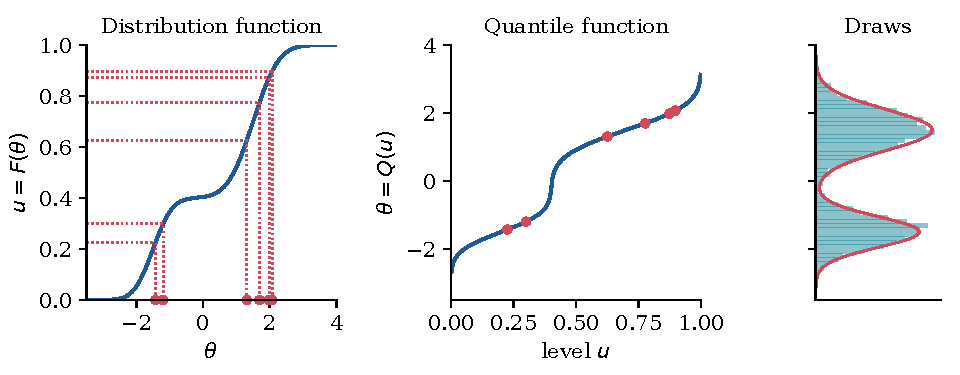
\includegraphics[width=\linewidth]{comp_inverse.pdf}
\caption{One bimodal posterior, the mixture $0.4\,N(-1.5,0.45^2)+0.6\,N(1.5,0.6^2)$. Left: its distribution function, with six uniform draws carried across to the curve and down to draws of $\theta$. Centre: the quantile function. Right: 5{,}000 draws $Q(U)$ and the exact density.}
\label{comp:fig:inverse}
\end{figure}

For a vector $\theta=(\theta_1,\ldots,\theta_d)$ we apply the scalar statement one coordinate at a time, with independent uniforms $U_1,\ldots,U_d$:
\[
\theta_1 = G_1(U_1,s),\qquad \theta_j = G_j(U_j,s,\theta_1,\ldots,\theta_{j-1}),\quad j=2,\ldots,d,
\]
where $G_j$ is the quantile function of $\theta_j$ given $s$ and the earlier coordinates. The map is triangular\index{triangular map|textbf}. It is the factorization $p(\theta_1\mid s)\,p(\theta_2\mid s,\theta_1)\cdots$ turned into a sampler, which transport theory calls the Knothe and Rosenblatt map\index{Knothe Rosenblatt map|textbf} (Rosenblatt 1952; Knothe 1957). Brenier's theorem (Brenier 1991) gives a different map, the gradient of a convex function; the two generally differ, coinciding when the coordinates are independent. For computation any map with the right output law will do, and the triangular one reduces a vector problem to $d$ scalar quantile regressions.

Every coordinate order gives an exact generator, but early errors pass to later coordinates. We put the quantity of interest first, learning the treatment effect from its marginal posterior given the summary before the nuisances. No ordering repairs bias from a prior that ignores the propensity score (Section~\ref{comp:sec:core}).

The theorem allows atoms. A spike and slab posterior puts positive probability on a coefficient being exactly zero, and its quantile function has a flat piece at zero whose length on the level axis is that probability. The horseshoe posterior has a density, so its quantile function has no flat piece.

Pushing several coordinates through their own marginal quantile functions with one shared $U$ gives the right margins and the wrong joint law: the coordinates become comonotone, perfectly rank correlated whatever the posterior says. Driving the treated and control quantile functions with one uniform is the same mistake in causal dress, and it assumes rank preservation\index{rank preservation} (Section~\ref{sec:ot}).

One map serves every question through an identity. As $G(U,s)$ with $U$ uniform on $(0,1)^d$ has the posterior law, for any $h$ with $\E\lvert h(\theta)\rvert<\infty$
\begin{equation}\label{comp:eq:quantileidentity}
\E\{h(\theta)\mid s\} = \int_{(0,1)^d} h\bigl(G(u,s)\bigr)\,du.
\end{equation}
For $d=1$, $h(\theta)=\theta$ gives the posterior mean as the area under the quantile function\index{quantile function}, and $h(\theta)=\one(\theta>c)$ gives the posterior probability of $\theta>c$ as the share of levels at which the quantile function exceeds $c$. The Wasserstein-1 distance between two scalar posteriors is the area between their quantile functions. A utility is another $h$. A risk criterion reweights the levels of the utility's own quantile function (Chapter~\ref{ch:cdt}): for scalar $\theta$ that is the utility of the quantile function of $\theta$ only when the utility increases in $\theta$, and in general the utilities of the draws are sorted first. Once $G$ is learned a new question costs an integral, not a new fit: the learned map is the model, and each integral is accounting (Chapter~\ref{ch:mccullagh}).

% comp section 04 (comp:sec:network, gbc:sec:qnn), phase 2 rewrite; "The proposition is exact" is in comp/s06, "A check that can be run" in comp/s09
\section{Learning the map: the check loss and the quantile network}\label{gbc:sec:qnn}\label{comp:sec:network}

We cannot write $G$ down, but regression on simulated pairs of parameter and summary learns a conditional mean under squared error and a conditional quantile under the check loss\index{check loss|textbf}; give the network the level as an input and it learns every quantile at once.

\subsection{The quantile neural network}

A quantile neural network\index{quantile neural network|textbf} is a function $f_\phi(u,s)$ of a level $u\in(0,1)$ and a value $s$ of the summary. We train it on simulations from the prior predictive distribution: draw $\theta^{(j)}\sim\pi$ and $D^{(j)}$ from the model, set $s^{(j)}=S(D^{(j)})$, draw a level $u_j$ uniformly, and minimize the check loss\index{quantile neural network!training by check loss|textbf}
\begin{equation}\label{gbc:eq:pinball}
\mathcal L(\phi) = \frac1J\sum_{j=1}^J \rho_{u_j}\bigl(\theta^{(j)} - f_\phi(u_j, s^{(j)})\bigr),\qquad \rho_u(r) = r\{u - \one(r<0)\}.
\end{equation}
At inference $f_\phi(V,s)$ with $V$ uniform and $s=S(D^{\mathrm{obs}})$ is an approximate posterior draw. For a vector $\theta$ the loss is applied coordinate by coordinate in the triangular order, with the earlier coordinates added to the inputs.

\begin{proposition}[What the check loss learns]\label{gbc:prop:pinball}
Let $(\theta, S)$ have the joint law induced by the prior and the model, with $\E\lvert\theta\rvert<\infty$, and let $U$ be uniform and independent of them. Among measurable functions $f(u,s)$ with $\E\lvert f(U,S)\rvert<\infty$, the expected check loss $\E\,\rho_U(\theta - f(U,S))$ is minimized by $f^\ast(u,s) = Q(u\mid s)$, the conditional quantile function of $\theta$ given $S=s$, and the minimizer is unique for almost every $(u,s)$ at which the conditional distribution function is strictly increasing.
\end{proposition}
\begin{proof}
Conditioning on $(U,S)$, it suffices to minimize $g(q) = \E[\rho_u(\theta - q)\mid S=s]$ over $q$. The function $g$ is convex with right derivative $F(q\mid s) - u$, which is nonnegative exactly when $q\ge Q(u\mid s)$, so the minimum is attained at the conditional $u$ quantile, uniquely where $F(\cdot\mid s)$ is strictly increasing. Integrating over $(u,s)$ gives the result.
\end{proof}

The proposition is about the population minimizer. For a trained network the evidence is the checks of Section~\ref{comp:sec:checks}. Integrated over $u$, the check loss of a curve that increases in $u$ is half the continuous ranked probability score\index{continuous ranked probability score|textbf}\index{CRPS|see{continuous ranked probability score}} of the law the curve describes, a strictly proper score (Gneiting and Raftery 2007). 

\subsection{Quantile neural networks explained}\label{gbc:sec:qnnexplained}

The check, or pinball\index{pinball loss|see{check loss}}, loss charges $u$ per unit when the target lies above the guess and $1 - u$ when below, so the guess that balances the two expected charges is the $u$ quantile (Figure~\ref{fig:qnnloss}). Classical quantile regression fits one level at a time (Koenker and Bassett 1978). The implicit quantile network of Dabney, Ostrovski, Silver and Munos (2018), introduced for distributional reinforcement learning, takes the level as an input, so one network\index{quantile neural network} represents the whole quantile function $u \mapsto Q(u \mid s)$.

\begin{figure}[ht]
\centering
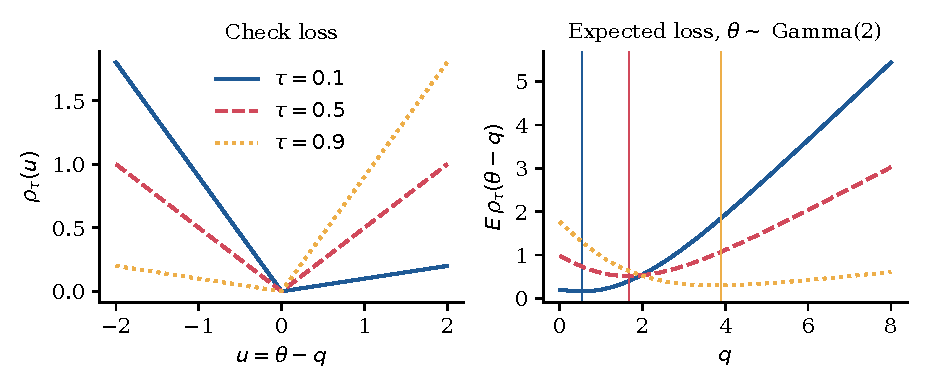
\includegraphics[width=\linewidth]{qnn_loss.pdf}
\caption{Left: the check loss for levels 0.1, 0.5 and 0.9. Right: expected check loss for a Gamma(2) target; the minimizers, marked by vertical lines, are the 0.1, 0.5 and 0.9 quantiles.}
\label{fig:qnnloss}
\end{figure}

\paragraph{The architecture.} In Figure~\ref{fig:qnnarch} the level enters through a cosine embedding, $\cos(i\pi u)$ for $i = 1, \ldots, K$ with $K = 32$, followed by one layer, and the summary passes through two layers. The two embeddings, each of width 64, are multiplied coordinate by coordinate, so that the shape of the posterior, not only its location, can change with $s$, and a two layer head returns the quantile. The two examples of this section train on the check loss alone, with inputs and outputs on their own scales. The worked example of Section~\ref{comp:sec:core} also uses the check loss alone but standardizes inputs and targets by their training means and standard deviations. The horseshoe networks of Section~\ref{comp:sec:horseshoe} use the defaults of the \texttt{gbc} package (Polson and Sokolov 2023), which add an L1 location anchor and a soft penalty on crossing quantiles to the check loss and normalize inputs and outputs.

\begin{figure}[ht]
\centering
\resizebox{\linewidth}{!}{\begin{tikzpicture}[node distance=5mm and 7mm, box/.style={draw,rounded corners=2pt,minimum height=7mm,inner sep=3pt,font=\small,align=center}, ar/.style={-{Stealth[length=2mm]}}]
\node[box] (tau) {$u \sim U(0,1)$};
\node[box, right=of tau] (cos) {cosine\\ embedding};
\node[box, right=of cos] (lt) {layer};
\node[box, below=9mm of tau] (h) {summary $S(D)$};
\node[box, right=of h] (lh1) {layer};
\node[box, right=of lh1] (lh2) {layer};
\node[circle,draw,inner sep=1pt, right=12mm of $(lt)!0.5!(lh2)$] (prod) {$\odot$};
\node[box, right=7mm of prod] (head) {head};
\node[box, right=7mm of head] (q) {$\theta = f_\phi(u, s)$};
\draw[ar] (tau) -- (cos); \draw[ar] (cos) -- (lt); \draw[ar] (lt) -| (prod);
\draw[ar] (h) -- (lh1); \draw[ar] (lh1) -- (lh2); \draw[ar] (lh2) -| (prod);
\draw[ar] (prod) -- (head); \draw[ar] (head) -- (q);
\end{tikzpicture}}
\caption{The quantile neural network. The quantile level and the data summary are embedded separately, combined by a coordinatewise product $\odot$, and mapped to a quantile of the posterior.}
\label{fig:qnnarch}
\end{figure}

\paragraph{Training and sampling.}  Each pass pairs every simulated summary with four fresh uniform levels, in minibatches of 512 simulations, and takes Adam steps on \eqref{gbc:eq:pinball} at learning rate $0.002$ with a cosine decay, for 60 passes. Averaging the network over a grid of levels gives the posterior mean by \eqref{comp:eq:quantileidentity}. Reweighted averages give the distorted values and risk criteria of Section~\ref{gbc:sec:risk} when the utility increases in $\theta$; otherwise they reweight the sorted utilities of the draws.

\paragraph{Crossing and rearrangement.} Nothing forces $f_\phi(u,s)$ to increase in $u$, so a curve read off a grid of levels can cross. Sorting it costs nothing: by the rearrangement inequality\index{rearrangement inequality|textbf} of Hardy, Littlewood and P\'olya (1952) it never raises the integrated check loss at any outcome, nor, by Chernozhukov, Fern\'andez Val and Galichon (2010), the error in estimating a monotone function. Draws $f_\phi(V,s)$ with $V$ uniform already follow the sorted curve, since the law of $f(V)$ has the increasing rearrangement of $f$ as its quantile function, so quantities computed from draws are unaffected. The curves of Figure~\ref{fig:qnnnormal} and the errors reported below are for the raw network output, so sorting could not raise them. 

\paragraph{Normal learning, learned.} Take $\theta \sim N(0, 1)$ and ten observations $y_i \mid \theta \sim N(\theta, 1)$, with the sufficient summary $S = \bar y$. The exact posterior is normal with mean $10\bar y/11$ and standard deviation $1/\sqrt{11} \approx 0.302$. We trained the network on 40{,}000 prior simulations. Figure~\ref{fig:qnnnormal} compares the learned and exact quantile functions at three values of $\bar y$: the mean absolute error over a grid of 99 levels from 0.01 to 0.99, which approximates the Wasserstein distance between learned and exact posteriors, is between 0.007 and 0.013. At $\bar y = 1.5$, 20{,}000 draws from the network have mean 1.359 and standard deviation 0.300, against exact values of 1.364 and 0.302.

\begin{figure}[ht]
\centering
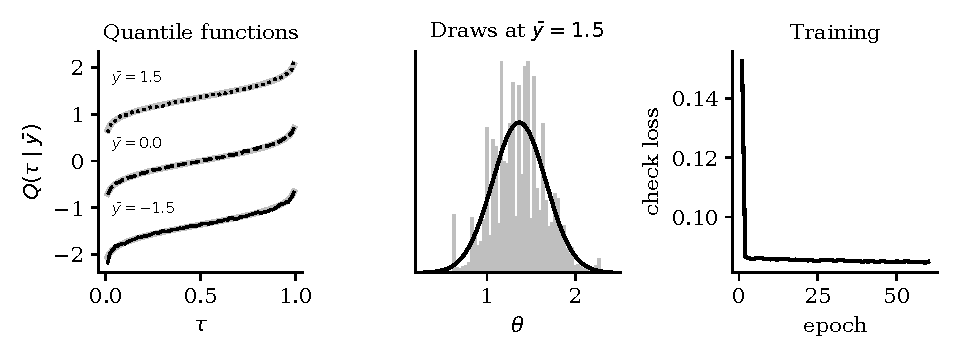
\includegraphics[width=\linewidth]{qnn_normal.pdf}
\caption{Normal learning with a quantile neural network. Left: learned quantile functions (thin lines) and exact posterior quantile functions (thick grey lines) at $\bar y = -1.5$, $0$ and $1.5$. Centre: network draws at $\bar y = 1.5$ against the exact posterior density. Right: the training loss.}
\label{fig:qnnnormal}
\end{figure}

\paragraph{A randomized trial, learned.} Take a two arm trial with 50 patients per arm, success probabilities $p_0$ and $p_1$ with independent uniform priors, and target the risk difference $\tau = p_1 - p_0$. The summary is the pair of observed success rates. We trained on 60{,}000 simulated trials and evaluated the network at 18 control and 27 treated successes. The exact posterior is a difference of two beta variables. The network gives a posterior median of 0.172 and a 90\% interval of $[0.019, 0.332]$; the exact values are 0.174 and $[0.014, 0.328]$. The posterior probability that treatment helps is 0.967 from the network and 0.963 exactly. Figure~\ref{fig:qnntrial} shows both posteriors and a simulation based calibration over 500 simulated trials with 19 draws each; in the saved run, which used two threads, the rank histogram is consistent with uniformity, with a chi squared statistic of 22.2 on 19 degrees of freedom, a value that changes with the thread count.

\begin{figure}[ht]
\centering
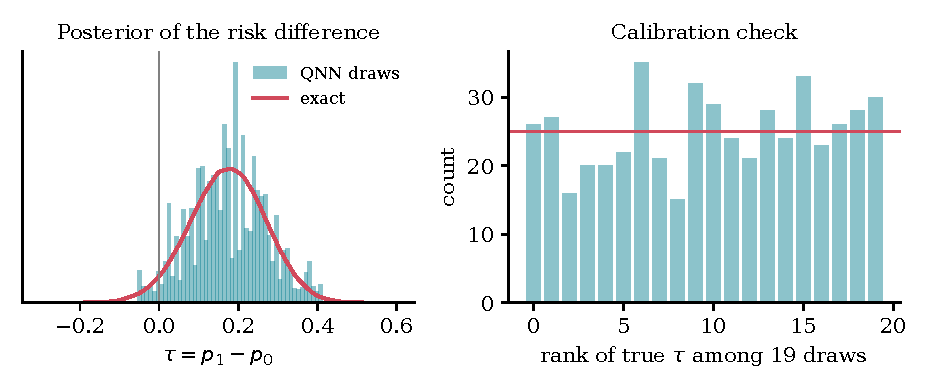
\includegraphics[width=\linewidth]{qnn_trial.pdf}
\caption{A two arm trial. Left: network draws of the risk difference at 18 of 50 and 27 of 50 successes, against the exact posterior. Right: ranks of the true risk difference among 19 network draws, over 500 simulated trials; the line is the count expected under perfect calibration.}
\label{fig:qnntrial}
\end{figure}



% comp 05: the algorithm and what it costs; phase 2 rewrite of the moved m14 and m16 text
\section{The algorithm and what it costs}\label{comp:sec:algorithm}\label{gbc:sec:algorithm}

Everything the network knows about the model comes from simulations: the algorithm\index{generative Bayesian computation!algorithm|textbf} is a table of simulated pairs and one regression on it.

\begin{enumerate}[leftmargin=*]
\item \emph{Simulate.} For $j=1,\dots,J$, draw $\theta^{(j)}$ from the prior and a data set $D^{(j)}$ from the model at $\theta^{(j)}$.
\item \emph{Summarize.} Compute $s^{(j)}=S(D^{(j)})$ for every simulated data set, with the code later applied to the observed data.
\item \emph{Train.} Draw levels $u_j$ uniformly on $(0,1)$ and fit $f_\phi$ by minimizing the check loss \eqref{gbc:eq:pinball} over the triples $(\theta^{(j)},u_j,s^{(j)})$, coordinate by coordinate in triangular order if $\theta$ is a vector (Section~\ref{gbc:sec:qnn}).
\item \emph{Infer.} Compute $s=S(D^{\mathrm{obs}})$, draw $U_1,\dots,U_R$ uniformly and return $\theta^{(r)}=f_\phi(U_r,s)$. For a vector $\theta$, draw an independent uniform for each coordinate and evaluate the maps in triangular order, each given the coordinates already drawn.
\end{enumerate}

The $R$ draws approximate the posterior of $\theta$ given $S=s$ (Section~\ref{comp:sec:summaries}); they follow it exactly only if $f_\phi$ is the conditional quantile function, and Section~\ref{comp:sec:checks} says how to test how close it is. 

Training costs $C_{\mathrm{train}}$ for steps 1 to 3; step 4 costs $C_{\mathrm{net}}$ per data set, including $R$ forward passes. A sampler costs $C_{\mathrm{mcmc}}$ per data set. The network is cheaper for $n_{\mathrm{sets}}$ data sets when
\[
C_{\mathrm{train}} + n_{\mathrm{sets}}\,C_{\mathrm{net}} < n_{\mathrm{sets}}\,C_{\mathrm{mcmc}}
\quad\Longleftrightarrow\quad
n_{\mathrm{sets}} > \frac{C_{\mathrm{train}}}{C_{\mathrm{mcmc}} - C_{\mathrm{net}}},
\]
which is close to $C_{\mathrm{train}}/C_{\mathrm{mcmc}}$ when a forward pass costs far less than a chain.

The ten networks of Section~\ref{comp:sec:horseshoe} each took more than an hour to train, so $C_{\mathrm{train}}>10\times3{,}600=36{,}000$ seconds. Break-even is about 57{,}000 data sets at 0.63 seconds per horseshoe fit, 116{,}000 at 0.31 seconds (Section~\ref{comp:sec:cost}) and 440{,}000 at 0.081 seconds (40.6 seconds for 500 data sets, Section~\ref{comp:sec:horseshoe}), or more. The timings come from different machines, so these are orders of magnitude: the sampler wins unless there are at least tens of thousands of data sets.



For a new $s$, rejection ABC\index{approximate Bayesian computation|textbf}\index{ABC|see{approximate Bayesian computation}} keeps the fraction $a$ of the stored summaries nearest to $s$ and reads the posterior off their $\theta^{(j)}$. That is a local, nearest neighbour estimate of the conditional quantile function at $s$ that needs a tolerance and discards $(1-a)J$ simulations at every data set. The network is one global fit to all $J$ pairs. For rejection ABC with the tolerance balanced against Monte Carlo variance, the expected quadratic loss of the posterior mean exceeds its limit by a term of order $J^{-4/(4+k)}$ in the summary dimension $k$ (Fearnhead and Prangle 2012).  No theorem covers a network trained at random levels by stochastic gradient descent, so we claim no advantage in rate.

A network is trusted only where it has seen summaries: outside the simulated region, or where simulations are sparse, it extrapolates and the training loss does not flag it (Section~\ref{comp:sec:checks}).



% comp 06: summaries; phase 2 rewrite (the opening justification sentence of the old SPLIT paragraph is dropped; comp/s04 now says what the proposition gives)
\section{What the network sees: summaries}\label{comp:sec:summaries}

The network never sees the data. It sees $S(D)$, a vector we chose, and learns $\pi(\theta\mid S=s)$ (Proposition~\ref{gbc:prop:pinball}). A summary\index{summary statistics|textbf} is a promise about what we are willing to forget. If $S$ is sufficient the promise costs nothing; if not, this valid posterior conditions on less than the data and is less concentrated on average over data sets. Summarizing is the first of two approximations to $\pi(\theta\mid D^{\mathrm{obs}})$; the second is finite training.

Sufficient summaries lose nothing, as in the normal mean and the two arm trial of Section~\ref{gbc:sec:qnnexplained}, but when the support does not depend on $\theta$, a sufficient statistic of fixed dimension exists, under regularity conditions, only for exponential families. Learned summaries start from Fearnhead and Prangle (2012), who take $S(D)=\E[\theta\mid D]$ and estimate it by regressing simulated $\theta$ on simulated data. By the tower property the posterior given this summary keeps the full posterior mean, and its variance is the average of the full posterior variances over data sets sharing the summary. 

The posterior mean can carry no information. If the prior and the likelihood are unchanged when $\theta$ is replaced by $-\theta$, the posterior is symmetric about zero, typically with a mode on each side, and $\E[\theta\mid D]=0$ for every $D$, so the Fearnhead and Prangle summary is a constant and the network returns the prior. Coverage on held out simulations does not reveal the failure, since intervals from $\pi(\theta\mid S)$ have their nominal coverage over the prior predictive distribution\index{prior predictive distribution|textbf} for every $S$, and the global and local ranks of Section~\ref{comp:sec:checks} are flat for a network that returns the prior. The held out loss against a network given another summary shows it, and so does a reference posterior at the observed summary.

The third kind puts in what a frequentist would compute. For a binary treatment a natural choice collects the weighted outcome means, the covariate sums by arm divided by $N$ (the arm means times the arm shares) and the covariate second moments,
\[
\begin{split}
S(D) = \Bigl(&\tfrac1N\textstyle\sum_i \tfrac{W_iY_i}{\hat e(X_i)},\ \tfrac1N\sum_i\tfrac{(1-W_i)Y_i}{1-\hat e(X_i)},\\
&\tfrac1N\textstyle\sum_i X_iW_i,\ \tfrac1N\sum_i X_i(1-W_i),\ \tfrac1N\sum_i X_iX_i^\top\Bigr),
\end{split}
\]
to which one adds outcome regression coefficients by arm, treated and control means within propensity strata and any consistent estimator of the target. The first two components are inverse probability weighted outcome means (Chapter~\ref{ch:ipw}), whose difference is the Horvitz and Thompson estimate of the average effect. The covariate sums record imbalance; the second moments let the network learn its importance for the outcome model.

Fit $\hat e(X)$ inside $S$ on every simulated data set. If the observed analysis cross fits its nuisances, repeat that cross fit inside every simulated $S$, at the cost of nuisance fits on all $J$ data sets, so the network learns the law of the statistic it will see.

Chapter~\ref{ch:blp} proves what a good summary buys (Proposition~\ref{blp:prop:bvm}). Under regularity conditions the posterior given $S$ is asymptotically normal, centred at the efficient minimum distance estimator built from $S$. If $S$ contains an asymptotically normal estimator of a subvector of $\theta$, the summary posterior for that subvector is asymptotically at least as concentrated as the estimator, with a limiting covariance no larger in the matrix order. A good estimator of the target inside $S$ therefore bounds the loss from summarizing. The conditions include a smooth injective limit of $S$, a prior density continuous and positive at the truth, and conditions on the density of $S$, because convergence in distribution of $S$ does not by itself give convergence of the posterior given $S$. The result concerns the exact summary posterior, not a trained network.

No summary of a covariate can produce heterogeneity in $\tau(x)$ if the outcome model omits its interaction with treatment. Choose the summary with the model.

The second approximation is finite training: the network class, the optimizer and the number of simulations $J$. Padilla, Tansey and Chen (2022) give rates for quantile regression with ReLU networks, for an exact empirical risk minimizer at one fixed quantile level; for targets with compositional structure, an intrinsic dimension replaces the summary dimension $k$. Our network is trained at levels drawn at random, for which we know no rate. Theorem A.4 of Polson and Sokolov (2026a), proved there in outline, gives consistency for fully connected ReLU networks of the level and the summary: for a bounded parameter, summaries in a compact set, a H\"older continuous conditional quantile function and a width that grows slowly enough with $J$, the expected integrated check loss of the empirical minimizer converges to its infimum, the expectation being over the training set as well. It does not cover the product architecture of Section~\ref{comp:sec:network}, whose complexity we have not bounded, and none of it bounds the error of the stochastic gradient descent that trains the network.

% comp s07 (W4, phase 2): the causal core; log misc/work-orders/comp-phase2-W4.applied.md
\section{Posteriors of effects from simulated pairs}\label{gbc:sec:efficiency}\label{comp:sec:core}

The network does not know what an average treatment effect is. It learns the law of whatever the simulator puts in the target, given whatever it puts in the summary, so the causal content of the analysis is decided before training starts, by six decisions\index{generative Bayesian computation!posteriors of effects|textbf}.

\begin{enumerate}[leftmargin=*]
\item \emph{Choose the estimand.} The simulator draws both potential outcomes, so it can compute the model based effect (the average of $\tau(X_i;\theta)$ over the observed covariates), the sample effect (the average of the simulated $Y_i(1)-Y_i(0)$, whose observed halves are part of the simulated data) or the population effect. The posterior of the sample effect depends on the joint law assumed for the pair and need not be wider than that of the model based effect (Section~\ref{sec:imputation}).
\item \emph{Train on it.} Train on $\psi(\theta)$ for the model based or population effect, or the average simulated $Y_i(1)-Y_i(0)$ for the sample effect, to learn its marginal posterior directly. Alternatively, push joint draws of $\theta$ through $\psi$ using the triangular map (Section~\ref{comp:sec:noise}). Separate marginal networks lose dependence and give the wrong variance for functionals of correlated coordinates.
\item \emph{Learn the effect as a function.} Give the network $x$ as an input and draw $x$ at random in the simulator, or train at a grid. A joint statement about the curve needs joint draws of its values at the grid points, from a triangular map over the points (Section~\ref{comp:sec:noise}) or from joint draws of $\theta$; independent levels at each point lose the dependence.
\item \emph{Put the estimator in the summary.} With an AIPW or H\'ajek estimate in $S$ (Chapter~\ref{ch:ipw}) the exact summary posterior is asymptotically at least as concentrated as the estimator (Section~\ref{comp:sec:summaries}). Cross fit its nuisances inside the simulator, since residuals on the training simulations are too small; in Chapter~\ref{ch:blp} cross fitting raised the average coverage of nominal 90 percent intervals from 0.85 to 0.94.
\item \emph{Simulate the confounding we fear.} Calibration on simulated data certifies the computation inside the simulator, not the simulator against the world. The prior predictive must contain confounding of the strength and form the application plausibly has, under the coupled prior of Chapter~\ref{ch:horseshoe}.
\item \emph{Check.} Run the checks of Section~\ref{comp:sec:checks}, against an exact reference where there is one.
\end{enumerate}

\paragraph{What holds.} In a correctly specified regular parametric model, with a prior positive and continuous at the truth and summaries that are sufficient or contain an efficient estimator, the Bernstein von Mises theorem gives a posterior that is asymptotically normal, centred at an efficient estimator, with the inverse Fisher information as variance. By the delta method any smooth functional, such as an average effect $\tau_Q(\theta)$, then has a posterior efficient for that model, and the network inherits this up to its training error, which no theorem bounds.

\paragraph{What does not hold automatically.} Semiparametric efficiency, the bound of Hahn (1998) for the nonparametric model of the regression and the propensity score, attained by the estimator of Hirano, Imbens and Ridder (2003), is another matter. A prior that ignores the propensity score can concentrate around the right regression function and still give an average effect biased at the $\sqrt N$ scale, when the regression is rough and the propensity informative (Ray and van der Vaart 2020), and a shrinkage prior can produce regularization induced confounding (Hahn and coauthors 2018). Generative computation changes how the posterior is computed, not which posterior it is: with such a prior every map returns the same wrong posterior. The repair is in the prior or in the estimator: Chapter~\ref{ch:horseshoe} couples the prior to the treatment model, with the limits that chapter reports for large $p$, and Section~\ref{sec:baipw} puts the horseshoe inside the doubly robust score of DML.

\subsection{A worked example with an exact posterior}

The test model is the stylized supplement trial of Chapter~\ref{ch:cdt}, after the Lanarkshire milk experiment (Section~\ref{sec:milk}): $n=200$ children with a baseline measure of undernourishment $Z_i\sim N(0,1)$ and a supplement $W_i$ given with probability $\expit(1+0.8Z_i)$. Covariates and assignments are drawn once and held fixed: 140 treated and 60 control children, with mean $Z$ of 0.26 and $-0.72$ respectively. The outcome is $Y_i=\mu_w+\alpha_wZ_i+\varepsilon_i$ for $w=W_i$, with $\varepsilon_i\sim N(0,1)$ and the variance known, and $\theta=(\mu_0,\alpha_0,\mu_1,\alpha_1)$ has the prior $N(0,4I)$. The targets are the model based effect $\psi=(\mu_1-\mu_0)+(\alpha_1-\alpha_0)\bar Z$, with $\bar Z$ the mean of the $Z_i$, and the conditional effect $\tau(z)=(\mu_1-\mu_0)+(\alpha_1-\alpha_0)z$.

The four within arm least squares coefficients $S$ are sufficient, so every network error is amortization error (Section~\ref{comp:sec:checks}). The arms have independent normal posteriors: with design $B_w$ (rows $(1,Z_i)$) and least squares coefficients $b_w$,
\[
(\mu_w,\alpha_w)^\top\mid S \sim N\bigl(V_wB_w^\top B_wb_w,\ V_w\bigr),\qquad V_w=\bigl(B_w^\top B_w+\tfrac14 I_2\bigr)^{-1}.
\]
The covariance depends only on the fixed design, so the exact posterior sd of $\psi$, the square root of $(1,\bar Z)(V_0+V_1)(1,\bar Z)^\top$, is 0.179 at every data set, against a prior sd of 2.83.

The ATE network is the quantile network of Section~\ref{comp:sec:network} with $\psi(\theta)$ as the target, trained with the check loss on 100,000 simulated pairs of $\theta$ and $S$ for 40 passes, about 26 seconds on two threads of an Intel server node. The observed data set is one draw of $\theta$ from the prior and the data simulated at it; the checks use 500 fresh studies with 100 draws each and 20,000 fresh pairs. Each network was trained once, so the observed data set results are for one data set and one seed.

At the observed data set the exact posterior of $\psi$ has mean 0.079 and sd 0.179, and 20,000 draws from the network have mean 0.067 and sd 0.185. Their Wasserstein-1 distance is 0.015, or 0.085 of the posterior sd (Figure~\ref{comp:fig:ate}a and c).

\begin{figure}[ht]
\centering
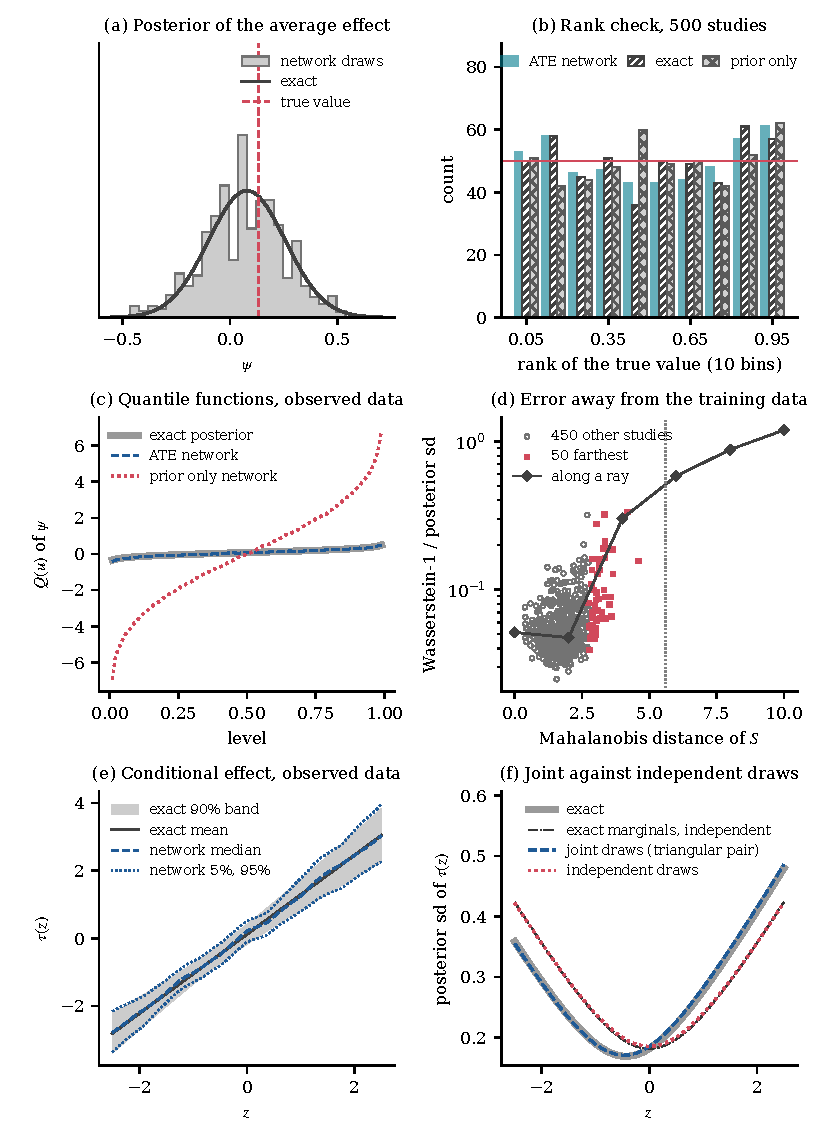
\includegraphics[width=\linewidth,trim=0bp 185bp 0bp 0bp,clip]{gbc_ate.pdf}
\caption{The ATE network of the worked example. (a) Draws of $\psi$ at the observed data set, the exact posterior density and the true value (dashed line). (b) Rank histograms over 500 studies for the ATE network, the exact posterior and the prior only network (trained with the summary replaced by a constant); the line marks the expected count of 50. (c) Quantile functions of the same three at the observed data set. (d) Wasserstein-1 error over the exact posterior sd against the Mahalanobis distance of $S$ from the center of the training summaries, for the 500 studies (the 50 farthest as squares) and along a ray leaving the center in the direction in which the exact mean of $\psi$ moves fastest; the dotted line is the largest distance among the training summaries.}
\label{comp:fig:ate}
\end{figure}

The rank check over 500 studies (Table~\ref{comp:tab:ate}, Figure~\ref{comp:fig:ate}b) cannot tell the ATE network from the exact posterior. Nor can it tell either from a prior only network, which is trained with the summary replaced by a constant and has intervals about 16 times as wide. The held out loss can: it puts the prior only network at 0.798 against 0.050 for the exact quantile function, and resolves the ATE network's excess, 0.00024, at 8.9 standard errors.

\begin{table}[ht]
\centering
\caption{Checks of three posteriors for $\psi$. Ranks: 500 studies with 100 draws each, in ten bins. Intervals run between the 5th and 95th percentiles of the draws (Weibull plotting positions). Held out loss: the check loss on 20,000 fresh pairs with eight random levels each, for the exact quantile function and for the raw network function (0.05027 for the ATE network after sorting).}
\label{comp:tab:ate}
\footnotesize\setlength{\tabcolsep}{4pt}
\begin{tabular}{L{1.2in}>{\raggedleft\arraybackslash}p{0.8in}>{\raggedleft\arraybackslash}p{0.55in}>{\raggedleft\arraybackslash}p{0.55in}>{\raggedleft\arraybackslash}p{0.6in}}
\toprule
 & Rank $\chi^2$ ($p$) & Coverage of 90\% & Width of 90\% & Held out loss \\
\midrule
Exact posterior & 10.12 (0.341) & 0.876 & 0.603 & 0.05012 \\
ATE network & 8.12 (0.522) & 0.870 & 0.601 & 0.05037 \\
Prior only network & 8.36 (0.498) & 0.882 & 9.514 & 0.79757 \\
\bottomrule
\end{tabular}
\end{table}

The 50 studies with summaries farthest from the training center (Mahalanobis distance) have a flat rank histogram and a Wasserstein-1 error of 0.110 of the exact sd, against 0.061 for the other 450, although all 500 lie inside the training range (largest distance 4.59, against 5.61 among the training summaries). Beyond that range, along the ray of Figure~\ref{comp:fig:ate}d, the error passes the posterior sd (1.19 of it at distance 10).

The CATE network, with $z$ as a further input drawn from $N(0,1)$ for each simulated pair, is less accurate than the ATE network at this data set: its Wasserstein-1 errors are 0.114, 0.531 and 0.128 of the exact sd at $z=-1.5$, 0 and 1.5 (Figure~\ref{comp:fig:cate}e).

The 0.531 is mostly one unlucky fit. We trained ten networks of each kind, differing in initial weights and minibatch order, at each of 10{,}000, 40{,}000, 100{,}000 and 400{,}000 simulated pairs (each training set a prefix of the next and the same for every seed, with the architecture and 40 passes above), and compared the sorted network quantiles on 999 levels from 0.001 to 0.999 with the exact posterior quantiles on 2{,}000 fresh studies, by the Wasserstein-1 error over the exact sd. Each network gives a median and a 90th percentile of this error over the studies and a coverage, and we report their means over the ten seeds.

At 100{,}000 pairs the CATE network at $z=0$ has median error 0.15 (0.14 at $z=-1.5$, 0.11 at $z=1.5$), 90th percentile 0.33 and coverage of 90 percent intervals 0.91. At the observed data set its error averages 0.15 over the ten seeds, with standard deviation 0.13 and largest value 0.49, so our single network, trained on a different draw of simulations, lies above all ten. The error falls roughly as $J^{-1/2}$, from a median of 0.60 at 10{,}000 pairs to 0.09 at 400{,}000. The ATE network is more accurate at every size, with median error 0.30 to 0.41 of the CATE network's at $z=0$ (0.054 at 100{,}000 pairs), so a conditional effect needs several times the simulations of an average one for the same accuracy.

\begin{figure}[ht]
\centering
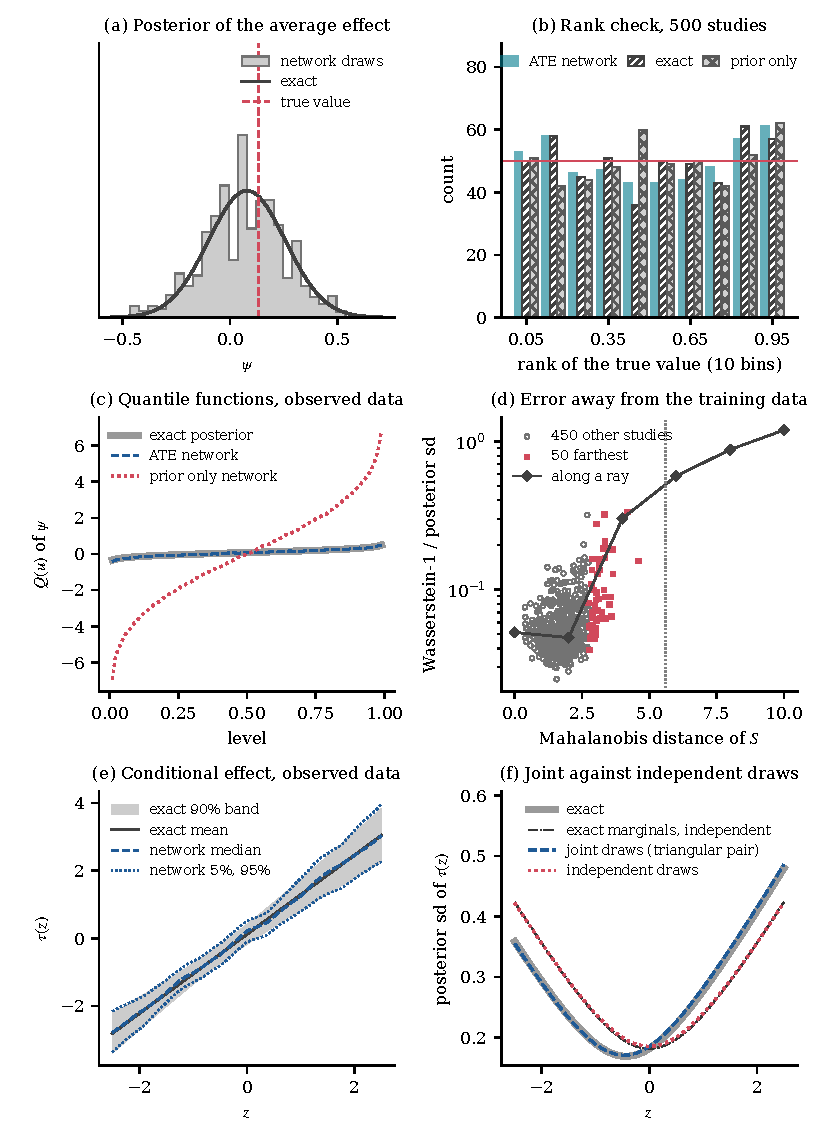
\includegraphics[width=\linewidth,trim=0bp 0bp 0bp 362bp,clip]{gbc_ate.pdf}
\caption{The conditional effect. (e) Exact posterior mean and 90 percent band of $\tau(z)$ at the observed data set, with the median and the 5 and 95 percent points of the CATE network. (f) Posterior sd of $\tau(z)$ from the exact posterior, from the exact marginals combined as if independent, from triangular draws and from independent draws.}
\label{comp:fig:cate}
\end{figure}

The second decision matters for the same curve. The exact posterior correlation of $\Delta\mu=\mu_1-\mu_0$ and $\Delta\alpha=\alpha_1-\alpha_0$ is 0.368. Triangular draws, from a network for $\Delta\mu$ and one for $\Delta\alpha$ given $S$ and the drawn $\Delta\mu$, have correlation 0.390; independent draws take $\Delta\alpha$ from a network given $S$ alone. At $z=-1.5$ and 1.5 the sd of $\tau(z)$ is 0.990 and 1.017 times the exact sd for triangular draws, 1.251 and 0.862 for independent draws, and 1.247 and 0.858 for the exact marginals combined as if independent: the fault is the lost dependence, not the networks (Figure~\ref{comp:fig:cate}f). We chose the assignment intercept so that the components are correlated: at intercept 0 the correlation is 0.001.

The example is narrower than the recipe: the summary is sufficient, the prior normal, the only confounder one observed covariate, and a network serves one design. It has no AIPW summary and no cross fitted nuisances, and we have not tried the coupled horseshoe prior with a network.

% comp section 08
\section{Learning the horseshoe posterior, and why we usually do not}\label{comp:sec:horseshoe}\label{gbc:sec:horseshoe}

The Gibbs sampler of Chapter~\ref{ch:horseshoe} fits a horseshoe regression in 0.31 seconds at $n = 200$ and $p = 51$ (Section~\ref{comp:sec:cost}), so a network has to earn its training time\index{generative Bayesian computation!horseshoe posterior|textbf}. In our book \emph{Generative Bayesian Computation} (Polson and Sokolov 2026a) we gave it a deliberately easy case: ten coefficients, a fixed design of $n = 50$ rows of independent standard normals, known error standard deviation $\sigma = 0.5$, and 80,000 draws from the prior with the data they imply. The least squares estimate $b$ is sufficient for the coefficient vector $\beta$ given the design and $\sigma$, so each network maps $b$ to the quantile function of one $\beta_j$. In this experiment $\beta_j \mid \lambda_j, \gscale \sim N(0, \lambda_j^2\gscale^2)$ with standard half Cauchy local and global scales, not multiplied by $\sigma$ as in Chapter~\ref{ch:horseshoe}. Each network has width 256 and was trained for 3,000 full batch epochs with the defaults of the \texttt{gbc} package, whose loss adds an L1 location anchor and a crossing penalty to the check loss; the reference Gibbs sampler kept 20,000 draws after discarding 2,000.

The first obstacle is scale. The horseshoe prior has tails at least as heavy as a Cauchy's, so under it $\beta_j$ has no mean and no variance. The sample standard deviations of the 80,000 draws run from 808 to 21,740, while the median of $|\beta_j|$ is 0.56. Standardizing by the training mean and standard deviation squashes 92 percent of the draws to within 0.01 of the mean on the standardized scale, and an error of 0.001 on the standardized scale is an error of at least 0.81 in $\beta_j$, more than the median of $|\beta_j|$.

Three pipelines differ only in scale. The raw pipeline maps $b$ to $\beta_j$. The asinh pipeline maps $\operatorname{asinh}(b)$ to $\operatorname{asinh}(\beta_j)$ and returns the quantiles of $\beta_j$ through $\sinh$. The residual pipeline maps $\operatorname{asinh}(b)$ to $\beta_j - b_j$ and adds $b_j$ back to the fitted quantiles. Only the residual target is easy to scale: given $\beta$, the error $b - \beta$ is normal with covariance $\sigma^2(X^\top X)^{-1}$, which does not depend on $\beta$, so $\beta_j - b_j$ is exactly normal under the prior predictive distribution, with standard deviations from 0.067 to 0.096 across the coefficients.

We fixed two criteria before the runs. A pipeline is calibrated if the central 90 percent interval of each of its ten networks contains $\beta_j$ in 85 to 95 percent of 2,000 new data sets. It agrees with the Gibbs sampler of Makalic and Schmidt (2016), whose own intervals, pooled over ten coefficients and 500 data sets, covered 89.9 percent, if for every coefficient the median over 500 data sets of the Kolmogorov and Smirnov distance between the two posteriors is below 0.05. No pipeline passed. Two raw networks returned intervals of zero width that never contained $\beta_j$, and the other eight were 17 to 88 times as wide as the sampler's. The asinh and residual pipelines were calibrated and still disagreed with the sampler, by median distances of 0.16 to 0.18 and 0.062 to 0.078. Coverage averaged over data sets can be right while the posterior for a given data set is wrong. The residual intervals came within 5 percent of the sampler's widths, but their posterior medians were only 1 to 7 percent closer to the truth than the least squares estimates.

The sampler was also far cheaper: 40.6 seconds on one core for the 500 data sets, run 100 at a time by a vectorized sampler, or 0.081 seconds each, while one network took more than an hour to train, so the ten networks of one pipeline cost what the sampler spends on more than 440,000 data sets. 

Training a coupled horseshoe network would mean drawing the local and global scales from half Cauchy distributions, shared between the treatment and outcome equations when the coupling is through scales; leaving $\tau$ and the coefficient of the propensity covariate unshrunk, with wide normal priors; and holding the design at the observed covariates, so that one network serves one study. With $p$ larger than $n$ the least squares estimate is not unique, but for a fixed design $X^\top Y$ is still sufficient for the coefficients given $\sigma$ (with $Y^\top Y$ added when $\sigma$ is unknown); it has $p$ coordinates, and reducing it brings back the choices of Section~\ref{comp:sec:summaries}. We have not tried a network on the coupled design of Chapters~\ref{ch:dml} and~\ref{ch:horseshoe} ($n = 200$, $p = 51$, five confounders).

% comp s09 (W6, phase 2); log misc/work-orders/comp-phase2-W6.applied.md
\section{Checks and failure modes}\label{comp:sec:checks}

A failing sampler leaves traces in its output; a trained network returns a smooth quantile function whatever it has learned, so it needs outside checks\index{generative Bayesian computation!checks and failure modes|textbf}.

Split $\hat R$\index{split R hat@split $\hat R$} and the effective sample size say whether a chain has settled, and are read for the effect, not only for the nuisance parameters. The posterior predictive check\index{posterior predictive check|textbf} asks whether the model could have produced the data on the summaries the effect depends on: outcome means by arm within propensity strata, residual variance by arm, and the tails.

For split $\hat R$, cut each chain in half. With $m$ draws per half, let $W$ be the mean variance within halves and $B$ be $m$ times the variance of half chain means. The posterior variance estimate and diagnostic are
\[
\widehat{\mathrm{var}}^{+}=\frac{(m-1)W+B}{m},\qquad \hat R=\sqrt{\frac{\widehat{\mathrm{var}}^{+}}{W}}.
\]
Values near 1 say the halves agree. The effective sample size is the number of draws divided by $1+2\sum_{k\ge1}\rho_k$, where $\rho_k$ is the autocorrelation at lag $k$ and the sum is truncated as in Geyer's initial positive sequence. The Monte Carlo error of a posterior mean is about the posterior standard deviation over the square root of the effective sample size. For a probability of benefit, apply the same to $h=\one(\tau>0)$, which can mix differently from $\tau$, so a fixed number of sweeps does not fix the precision of a tail quantity.

Vehtari and coauthors (2021) replace the classical $\hat R$ by the larger of a rank normalized split $\hat R$ and its folded version, flag values above 1.01, and add a tail effective sample size from the indicators at the 5th and 95th percentiles; the checks of Section~\ref{sec:hsgibbs} used the classical versions. No diagnostic proves that every mode was visited.

Simulated pairs also test a network, in four checks (Figure~\ref{comp:fig:checks}).

\begin{figure}[ht]
\centering
\resizebox{\linewidth}{!}{\begin{tikzpicture}[node distance=7mm,box/.style={draw,rounded corners=2pt,minimum height=7mm,text width=2.3cm,inner sep=3pt,font=\small,align=center},ar/.style={-{Stealth[length=2mm]}}]
\node[box](a){held out loss};
\node[box,right=of a](b){global ranks};
\node[box,right=of b](c){local ranks at $s$};
\node[box,right=of c](d){reference};
\draw[ar](a)--(b);\draw[ar](b)--(c);\draw[ar](c)--(d);
\end{tikzpicture}}
\caption{The four checks of a trained network, in the order we run them.}
\label{comp:fig:checks}
\end{figure}

\paragraph{Held out check loss.} The first check meters the amortization\index{amortization|textbf} error, the distance at a summary $s$ between the network's posterior and the exact one. For a network that increases in $u$ (sorting, which never raises the loss, makes it so: Exercise~\ref{ex:chcomp:4}), averaging over the prior predictive\index{amortization} gives
\begin{equation}\label{comp:eq:amortization}
\E\int \{F_\phi(t \mid S) - F(t \mid S)\}^2\,dt = 2\{\bar{\mathcal L}(\phi) - \bar{\mathcal L}^\ast\}.
\end{equation}
Here $F_\phi(\cdot\mid s)$ is the distribution function of the draws $f_\phi(U,s)$, $\bar{\mathcal L}(\phi)=\E\,\rho_U\{\theta-f_\phi(U,S)\}$ is the expected check loss and $\bar{\mathcal L}^\ast$ its minimum, reached by the exact posterior. Held out pairs estimate $\bar{\mathcal L}(\phi)$ and so rank networks without a reference posterior, though an average can hide a large error at one summary.

\paragraph{Rank histograms.} The second check, the global ranks, ranks the true $\theta$ among $L$ draws from the network's posterior at $S(D)$: simulation based calibration\index{simulation based calibration|textbf}.

\begin{proposition}[Rank uniformity]\label{comp:prop:ranks}
Let $(\theta, D)$ come from the prior and the model\index{simulation based calibration}, with $\theta$ real valued, and let $S$ be any function of $D$. If the law of $\theta$ given $S$ has no atoms and, given $S$, the $L$ draws are independent of $\theta$ and of each other with that law, then the number $B$ of draws below $\theta$\index{rank statistic|textbf} is uniform on $\{0, \dots, L\}$.
\end{proposition}
\begin{proof}
Given $S$, $\theta$ and the $L$ draws are $L + 1$ independent draws from one law, hence exchangeable and almost surely distinct, so each of the $L + 1$ places $\theta$ can take in their order is equally likely: $\Prob(B = b \mid S) = 1/(L + 1)$ for every $b$.
\end{proof}

Even a network returning the prior has flat ranks and nominal held out coverage (Exercise~\ref{ex:chcomp:1}). The check certifies calibration\index{calibration|textbf} over the prior predictive, not sharpness or accuracy at the observed data. U shaped histograms mean draws too narrow; humped, too wide; tilted, shifted.

\paragraph{Local ranks.} The third check repeats the test at the observed summary $s$, for $M$ simulations and $M$ evaluations of the network: draw $M$ parameters from its posterior at $s$, simulate a data set from each, recompute the posterior, and rank the generating value. The test is not the same, however, because the parameters come from the posterior at $s$ and not from the prior: Proposition~\ref{comp:prop:ranks} does not apply, the local ranks of the exact posterior are not flat in general (in the normal example of Section~\ref{comp:sec:network} at $\bar y = 1.5$ about two thirds of them fall in the upper half), and those of a network that returns the prior are exactly flat at every $s$ (Exercise~\ref{ex:chcomp:1}). The check is informative when the prior is weak relative to the data, and with an informative prior it can pass a useless network and fail the exact posterior. In the trial, each draw of the risk difference $\tau$ is paired with $p_0$ from its conditional posterior given $\tau$ and the data, and $p_1 = p_0 + \tau$, with no clipping; a draw of $\tau$ outside $(-1, 1)$ has no valid pair and is redrawn. Importance weights proportional to likelihood times prior over network density target the exact posterior, provided these quantities are evaluable and the network density is positive on the posterior support; we have not tried this correction. 

\paragraph{Evidence.} We ran the local check with $M = 400$ and 19 draws each, at two threads, for a network retrained with the same design, at the observed trial of Section~\ref{gbc:sec:qnnexplained}, 18 of 50 and 27 of 50 successes, and at an extreme trial, 1 of 50 and 49 of 50. Against the exact posterior's expected counts under the same protocol, the network's counts give chi squared 21.1 on 19 degrees of freedom ($p = 0.33$) at the typical trial and 28.4 ($p = 0.08$) at the extreme one, so neither rejects agreement with the exact reference.

Against a flat histogram they give 24.0 ($p = 0.20$) and 222 ($p < 10^{-35}$). The extreme histogram piles up at the top ranks, but at so extreme a summary the exact posterior's own local ranks do so too, for the reason given above: with the exact posterior in place of the network, 200 repeats of the protocol give a chi squared statistic with median 20 at the typical trial and 244 at the extreme one. A direct comparison of the posteriors finds what the ranks miss. At the typical trial the network's posterior is within 0.003 of the exact one in Wasserstein distance; at the extreme trial it is shifted down and too wide, its 5\% quantile 0.834 against the exact 0.853 and its Wasserstein distance 0.009, because few training simulations land near a risk difference of 0.9 (Figure~\ref{fig:openlocalsbc})\index{simulation based calibration!local}. The global ranks of the network of Section~\ref{gbc:sec:qnnexplained} passed (chi squared 22.2 at two threads, Figure~\ref{fig:qnntrial}), since a risk difference above 0.9 has prior probability 0.005. Problem 6 of Chapter~\ref{ch:open} asks for a bound on such local error.

\begin{figure}[ht]
\centering
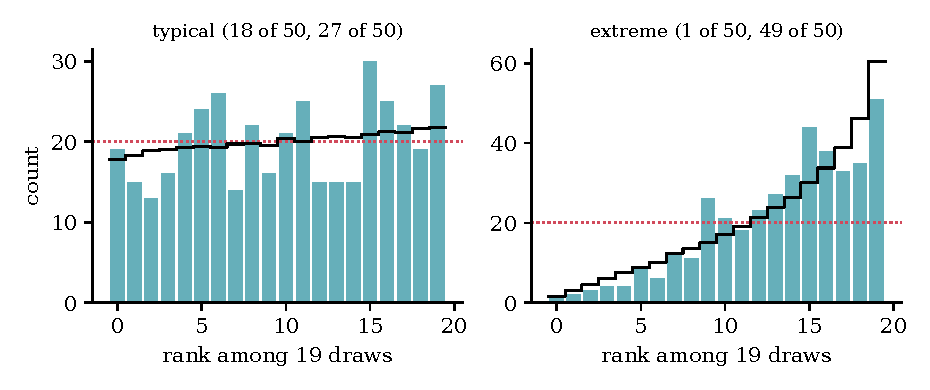
\includegraphics[width=\linewidth]{open_localsbc.pdf}
\caption{Local simulation based calibration of the trial posterior at a typical and an extreme data set: rank histograms of the network ($M = 400$ simulations, 19 draws each, network trained on 60{,}000 trials) per 400 draws, with the rank histogram of the exact posterior under the same protocol (black steps) and the flat count (dotted line).}
\label{fig:openlocalsbc}
\end{figure}

\paragraph{Reference.} Compare with a trusted posterior: the trial's beta difference, the normal posterior (Section~\ref{comp:sec:core}) or the horseshoe Gibbs sampler (Section~\ref{sec:hsgibbs}). The distance is local amortization error; the reference loss gives $\bar{\mathcal L}^\ast$. A tractable cousin tests the architecture, not the application.

Known failures, mostly from the experiments in our book \emph{Generative Bayesian Computation} (Polson and Sokolov 2026a):
\begin{itemize}
\item \emph{Under-dispersion.} On three of the four tasks we took from the benchmark of Lueckmann and coauthors (2021), separate networks trained with the check loss alone on 10,000 simulations gave central 90 percent marginal intervals that contained 31 to 52 percent of the true parameter components over the ten benchmark observations of each task (31 and 33 of 100, 26 of 50), for reasons not diagnosed.
\item \emph{High signal to noise.} Near deterministic outcomes, such as the luminosities of Chapter~\ref{ch:gente}, are the risk. The networks of that book gave intervals too wide in simulations and too narrow on its lake data set; for the narrow ones it offers only a heuristic, that the product of level and summary features starves the spread. Remedies: heteroscedastic ensembles, conformal calibration (marginal coverage only).
\item \emph{Lost dependence.} Separate networks give the marginals without the dependence, so a contrast gets the wrong variance (Exercise~\ref{ex:chcomp:2}), which only its own ranks reveal; the triangular map of Section~\ref{comp:sec:noise} keeps it.
\item \emph{Blurred jumps.} In surrogate regression of a response surface with a jump, averaging an ensemble blurs the jump, since its members place it at different points; one network given an estimated side of the jump did better. We have not tested a jump in a posterior or an outcome surface at a regression discontinuity.
\end{itemize}

% comp s10 (W6, phase 2); log misc/work-orders/comp-phase2-W6.applied.md
\section{Choosing the engine}\label{comp:sec:engine}

Table~\ref{tab:cost} compares engines and cost orders for $n$ units and $p$ covariates\index{engine choice|textbf}; constants depend on the machine.

\begin{table}[ht]
\centering
\caption{Engines by situation. $N_{\mathrm{it}}$ is the number of iterations and $J$ the number of simulated pairs.}
\label{tab:cost}
\footnotesize\setlength{\tabcolsep}{3pt}
\begin{tabular}{L{0.8in}L{0.62in}L{0.82in}L{1.0in}L{0.86in}}
\toprule
Situation & Engine & What it needs & How it fails & Cost order \\
\midrule
Gaussian outcome & Horseshoe Gibbs & Closed form full conditionals & Scales mix slowly & $np^2 + N_{\mathrm{it}}p^3$; $N_{\mathrm{it}}n^2p$ if $p > n$ \\
Binary or count outcome & Polya Gamma Gibbs & Logistic or count likelihood & As above & $N_{\mathrm{it}}(p^3 + np^2)$ \\
No closed form conditionals & HMC & Log posterior and its gradient & Funnels (divergences); heavy tails & $N_{\mathrm{it}}\times$ leapfrog steps $\times\, np$ \\
Near normal posterior & Laplace & Likelihood, gradients & Skewed or bounded posteriors, tails & One optimization and one Hessian \\
Speed, very large $n$ & Variational & Likelihood, a tractable family & Tails; error not reported & One optimization \\
Factorized family & Mean field & Independent blocks & Intervals too short & As variational \\
Likelihood unavailable or costly & Trained network & A simulator; no likelihood or gradients & Extrapolation, under-dispersion, lost dependence & $J$ simulations and a fit, then a forward pass per draw \\
One effect, no posterior & DML, $K$ folds & Cross fitted regressions & Interval only; needs overlap, nuisance rates & $2K$ cross validated lasso fits \\
\bottomrule
\end{tabular}
\end{table}

For Gaussian or Polya Gamma conditionals the Gibbs sampler is the default, and for the horseshoe Section~\ref{comp:sec:horseshoe} reports that trained networks lost to it. A network earns its training where the likelihood cannot be evaluated or is expensive, as in the merger studies of Chapter~\ref{ch:blp}, and over many data sets from one design\index{generative Bayesian computation!cost} (Section~\ref{comp:sec:algorithm} gives the break-even).

\section{In practice}

\paragraph{The target.} Every target in this book is a function of the draws $\theta^{(s)}$: an average effect is $\tau_Q(\theta^{(s)})$ for each draw, a merger threshold or a probability of causation another function of the same draws. The engine decides how fast the draws arrive and how closely they follow the posterior; the model, the prior and the summary decide which posterior that is.

\paragraph{What the analyst does differently.} For the horseshoe model she uses the fast sampler when $p$ exceeds $n$, and includes an unpenalized intercept or centres the outcome and every column. She runs 1,500 to 3,000 iterations, drops the first third, and reports split $\hat R$, the effective sample size for the effect and a posterior predictive check. For a network she reports the summary, the held out loss, the ranks of the effect, the local ranks and a reference where one exists.

\paragraph{Against DML.} DML is cheaper in principle, but in the two Gaussian outcome designs, with 51 and 56 columns and 200 and 9,915 units, we timed the horseshoe sampler at half the time of a cross fitted lasso and a twentieth of the time of a cross fitted forest (Section~\ref{comp:sec:cost}). As $p$ grows the factorization dominates and the comparison turns. In the replications of Section~\ref{sec:ricsim}, with $n = 200$, one coupled horseshoe fit, its lasso fit of the treatment included, took 1.6 seconds on average at $p = 150$ and 5.7 seconds at $p = 300$, while everything in a replication except its three horseshoe fits and the six lasso fits of the treatment that feed two of them, DML's ten lasso fits included, took 3.2 and 2.3 seconds, an upper bound on the cost of DML in that design. The reduced form sampler of Section~\ref{sec:crit:bayes} took 9.8 seconds for one chain of 2,000 sweeps at $n = 300$ and $p = 400$, and about 200 seconds for the four chains run to convergence that Table~\ref{tab:crit:head} uses, against 1.0 for a cross fitted lasso. We did not time the Polya Gamma sampler for a binary outcome, whose cost per iteration grows with $n$. DML with a lasso nuisance keeps a cost advantage at large $p$, and may keep one for a binary outcome and in a very large analysis with a nonlinear nuisance that a Gaussian or Polya Gamma model does not fit. In every design the posterior comes with checks for which DML has no counterpart. A trained network repays its training only over many data sets from one design.


\section*{Notes}
Noise outsourcing is a case of the transfer theorem of Kallenberg (2002); Villani (2009) treats optimal transport. Chernozhukov, Fern\'andez Val and Galichon (2010) show that sorting an estimated monotone function never raises its error in an $L^p$ norm. Learning a posterior as a quantile function of noise is the generative Bayesian computation of Polson and Sokolov (2023). Distributional reinforcement learning begins with Bellemare, Dabney and Munos (2017), and quantile regression for it is in Dabney, Rowland, Bellemare and Munos (2018).

Jiang and coauthors (2017) learned summaries with a neural network. Rank checks go back to Cook, Gelman and Rubin (2006) and were developed as simulation based calibration by Talts and coauthors (2018); Lueckmann and coauthors (2021) is the benchmark behind the under-dispersion result. That result, the other failure modes of Section~\ref{comp:sec:checks} and the consistency statement of Section~\ref{comp:sec:summaries} come from our book \emph{Generative Bayesian Computation} (Polson and Sokolov 2026a). The fast sampler for $p > n$ is Bhattacharya, Chakraborty and Mallick (2016), the simple horseshoe sampler Makalic and Schmidt (2016), and the Polya Gamma augmentation Polson, Scott and Windle (2013).

\begin{exercises}
\item\label{ex:ch14:1} Derive the Bhattacharya, Chakraborty and Mallick sampler for $N(A^{-1}Z^\top Y, \sigma^2 A^{-1})$, with $A = Z^\top Z + \Lambda^{-1}$ and $\Lambda$ diagonal as in Section~\ref{comp:sec:cost}, using the Woodbury identity.
\item\label{ex:ch14:2} Verify the Polya Gamma identity of Section~\ref{comp:sec:cost} for $b = 1$ by computing the Laplace transform of the Polya Gamma law defined in Appendix~\ref{app:toolkit}.
\item\label{ex:ch14:3} Show that, for a scalar parameter $\theta$ whose log posterior given $n$ observations $D$ is smooth with a unique interior mode, the Laplace approximation to the normalizing constant $\int p(D \mid \theta)\,\pi(\theta)\,d\theta$ has relative error $O(n^{-1})$ under regularity conditions. Show with a Gamma posterior that the normal approximation to the posterior density has relative error of order $n^{-1/2}$ at a fixed number of standard deviations from the mode.
\item\label{ex:ch14:4} Design summary statistics for an amortized posterior of the average treatment effect in a partially linear model, and argue for their approximate sufficiency.
\item\label{ex:ch14:5} Implement simulation based calibration for a proper version of the horseshoe regression of Section~\ref{sec:hsgibbs} with $n = 100$ and $p = 20$: a fixed design whose first column is a binary treatment and whose other columns are independent standard normals, the prior $\tau \mid \sigma^2 \sim N(0, 100\sigma^2)$ on the treatment coefficient in place of the flat one, the horseshoe on the other coefficients and an inverse gamma prior with shape 2 and scale 1 on $\sigma^2$, all used in the full conditionals. In each of 1,000 replications draw the parameters from this prior, simulate $Y$, run the sampler, keep 19 draws spaced far enough apart to be nearly independent for both $\tau$ and $\gscale$, and rank the generating values. Report the two rank histograms and how you checked the dependence of the kept draws.
\item\label{ex:chgbc:3} Let $Y_1, \ldots, Y_N$ be independent $N(\theta, \sigma^2)$ given $\theta$, with $\sigma$ known and $\theta \sim N(\mu_0, \sigma_0^2)$, as in the normal learning example of Section~\ref{gbc:sec:normal}. Given the summary $s = \bar Y$ the posterior of $\theta$ is $N(\mu_N(s), \sigma_N^2)$ with $\mu_N(s) = (\mu_0/\sigma_0^2 + Ns/\sigma^2)/(1/\sigma_0^2 + N/\sigma^2)$ and $\sigma_N^2 = (1/\sigma_0^2 + N/\sigma^2)^{-1}$. Verify that the check loss at level $u$ is minimized by $\mu_N(s) + \sigma_N\Phi^{-1}(u)$. Then, for the report $a^\ast = \mu_N(s)$ under the loss $(a^\ast-\theta)^2$, compute the mean of the upper 10\% of the loss over the posterior of $\theta$, which is the negative of the conditional value at risk (CVaR) at level 0.1 of the utility $-(a^\ast-\theta)^2$, the mean of the worst 10\% of that utility.
\item\label{ex:ch08:1} Prove Theorem~\ref{comp:thm:outsourcing} for real valued $Y$ by taking $G(u,x)$ to be the conditional quantile function, including laws with atoms.
\item\label{ex:ch08:2} Show that minimizing the expected check loss $\E\rho_u(Y - q)$ over $q$ gives the $u$ quantile of $Y$.
% comp exercises 1 to 4 (W6, phase 2), input by mcomp.tex inside the exercises environment
\item\label{ex:chcomp:1} In the normal example of Section~\ref{comp:sec:network} ($\theta \sim N(0, 1)$, ten observations $N(\theta, 1)$, summary $\bar y$), take a network that returns the prior $N(0, 1)$ at every summary. Show that its rank histogram is flat, over the prior predictive and at any observed summary. Then compute its expected check loss at level $u = 1/2$ and that of the exact posterior, and say which of the four checks of Section~\ref{comp:sec:checks} tell the two networks apart.
\item\label{ex:chcomp:2} At a covariate value $x$ the posterior draws of the two potential outcome means $\mu_1(x)$ and $\mu_0(x)$ have variances $v_1$ and $v_0$ and covariance $c$, which is not zero when the arms share parameters, as under a common prior scale. Show that independent draws of the two, as from separate networks, give $\mathrm{Var}\,\tau(x) = v_1 + v_0$ for $\tau(x) = \mu_1(x) - \mu_0(x)$, while joint draws give $v_1 + v_0 - 2c$. For which sign of $c$ do separate networks overstate the uncertainty about the effect, and how does the triangular map of Section~\ref{comp:sec:noise} repair it?
\item\label{ex:chcomp:3} Use the notation of Section~\ref{comp:sec:algorithm}. (a) The Gibbs sampler of Section~\ref{comp:sec:horseshoe} took 0.081 seconds per data set and training took at least $36{,}000$ seconds; taking $C_{\mathrm{net}}$ as negligible, how many data sets repay the training? (b) The local ranks of Section~\ref{comp:sec:checks} are run on every data set the network analyses and cost $C_{\mathrm{chk}}$ each. Show that the break-even becomes $C_{\mathrm{train}}/(C_{\mathrm{mcmc}} - C_{\mathrm{net}} - C_{\mathrm{chk}})$, and find the largest $C_{\mathrm{chk}}$ for which the network ever repays its training.
\item\label{ex:chcomp:4} Let $q$ be a measurable, integrable function on $(0, 1)$, $q^\ast$ its non-decreasing rearrangement (the quantile function of $q(V)$ for $V$ uniform) and $y$ a real number. Show that $\int_0^1 \rho_u\{y - q^\ast(u)\}\,du \le \int_0^1 \rho_u\{y - q(u)\}\,du$, using $\rho_u(y - q) = (q - y)_+ - u(q - y)$, the fact that $\int_0^1 (q(u) - y)_+\,du$ depends on $q$ only through the law of $q(V)$, and the rearrangement inequality of Hardy, Littlewood and P\'olya (1952), $\int_0^1 u\,q(u)\,du \le \int_0^1 u\,q^\ast(u)\,du$. Conclude that sorting the output of a network over $u$ never raises its expected check loss.

\end{exercises}

\chapter{Generative Treatment Effects and Joint Potential Outcomes}\label{ch:gente}

\begin{tcolorbox}[colback=gray!6,colframe=gray!50,title=In brief,fonttitle=\normalfont\itshape,coltitle=black,colbacktitle=gray!15,boxrule=0.4pt,arc=1pt]
Noise outsourcing represents any conditional law as a map from noise to outcomes. Learning that map for treated and untreated outcomes gives every conditional and quantile effect and every other functional of the two marginal laws, and decisions under concave utility need exactly these, not the average effect. The joint law of the two potential outcomes is a separate question: the marginals bound it without identifying it, and optimal transport supplies a canonical coupling, and a copula prior covers the rest.
\end{tcolorbox}

Average effects hide almost everything a decision maker needs. A drug that lowers mean blood pressure by five points might lower it by fifteen in a third of patients and do nothing for the rest. A tax credit that raises mean earnings might raise the lower quantiles and leave the upper ones alone. This chapter develops a generative approach to heterogeneous and distributional effects, built around the GenTE learner developed with Maria Nareklishvili. The object to learn is not a number but a map that turns noise, covariates and treatment into draws of the outcome.

\section{Conditional and distributional targets}

Under the strong ignorability\index{ignorability} of Chapter~\ref{ch:predictive}, which includes overlap, the conditional laws $F_t(\cdot \mid x)$ of $Y(t)$ given $X = x$ are identified for $t = 0, 1$ as the laws of $Y$ given $X = x$ and $T = t$. Every effect in the list below\index{distributional target} is a functional of this pair; effects that depend on the joint law of $Y(0)$ and $Y(1)$ are not, and Section~\ref{sec:ot} takes them up.
\begin{itemize}
\item The conditional average effect $\tau(x) = \int y\,dF_1(y \mid x) - \int y\,dF_0(y \mid x)$.
\item The conditional quantile effect\index{quantile treatment effect}\index{quantile treatment effect!conditional|textbf} at level $u$, $q_1(u \mid x) - q_0(u \mid x)$, where $q_t(\cdot \mid x) = F_t^{-1}(\cdot \mid x)$.
\item The unconditional quantile effect\index{quantile treatment effect!unconditional|textbf}, the difference of quantiles of the marginal laws $F_t = \int F_t(\cdot \mid x)\,Q(dx)$, which in general is not the average over $x$ of the conditional quantile effects, since the quantile of a mixture is not the mixture of the quantiles.
\item Effects on inequality measures, tail probabilities, or any other functional of the marginals.
\end{itemize}
In the terms of Chapter~\ref{ch:mccullagh}, the pair of conditional laws is the model and each of these is accounting; a method that learns the laws well can report all of them.

We therefore take the pair of conditional laws as the object to learn, and we need a representation of a conditional law that a learner can fit directly.

\paragraph{Noise outsourcing.} By Kallenberg's (2002) noise outsourcing\index{noise outsourcing} lemma (Theorem~\ref{comp:thm:outsourcing}), for random elements $(X, Y)$ in standard Borel spaces there are, on a possibly enlarged probability space, a measurable function $G$ and a random variable $U \sim \mathrm{Uniform}(0,1)$, independent of $X$, such that $Y = G(U, X)$ almost surely. For real valued $Y$ the function can be the conditional quantile function, $G(u, x) = F^{-1}(u \mid x)$, so learning $G$ is learning the whole conditional law. Chapter~\ref{ch:computation} learns posteriors as such maps; here we use the lemma for the outcome law itself.

This turns distribution learning into regression with one extra input: the network that fits $G$ takes $(u, x)$ and returns a quantile. Once it is fitted, every functional in the list above is computed by simulation: draw uniforms, evaluate $G$ at the covariates of interest under $t = 0$ and $t = 1$, and average the function of each arm's outputs that the question asks for, or, for a quantile, sort the outputs and read off the level. No density is written down and no integral is done by hand. A function of the two outputs together, such as the share of units whose treated draw exceeds their control draw, is another matter: feeding the same uniform to both arms couples them comonotonically, which is the rank preservation of Section~\ref{sec:ot}.

\section{The GenTE learner}

GenTE\index{GenTE|textbf}\index{generative treatment effects|see{GenTE}}, from Nareklishvili, Polson and Sokolov (2025), is a multihead feed forward network\index{GenTE!multihead network|textbf} with three jointly estimated subnetworks, propensity, baseline and treatment effect, each with its own covariate encoder. The propensity network produces a low dimensional embedding $e_\pi(x)$, which a logistic output layer turns into the propensity score\index{propensity score} $\hat e(x)$. The baseline network returns the conditional quantile function of the untreated outcome, $\mu(x, e_\pi(x), u) \approx q_0(u \mid x)$, and the effect network returns the quantile indexed treatment effect $\Delta(u \mid x) \approx q_1(u \mid x) - q_0(u \mid x)$. The model for the observed outcome is
\[
q_t(u \mid x) = \mu(x, e_\pi(x), u) + \Delta(u \mid x)\,t,
\]
and the conditional average effect is $\tau(x) = \int_0^1 \Delta(u \mid x)\,du$, since a mean is the integral of its quantile function.

The propensity embedding enters the baseline encoder and not the effect encoder, the neural counterpart of the propensity covariate of Chapter~\ref{ch:horseshoe} and of the Bayesian causal forest: the baseline cheaply represents outcome variation that moves with the propensity, so that variation is not pushed into the effect, the mechanism of regularization induced confounding. The effect is also a separate component, so regularization acts on it directly and can shrink it toward homogeneity.

Following the implicit quantile networks\index{implicit quantile network|textbf} of Dabney and coauthors (2018), a cosine embedding of $u$, built from $\cos(\pi iu)$ for $i = 1, \ldots, 32$, multiplies the covariate features elementwise before the output layer. The training loss combines a cross entropy term for treatment, the check loss
\[
\rho_u(r) = r\{u - \mathbf{1}(r < 0)\}
\]
for the observed outcome at a randomly drawn quantile level, and a penalty that discourages quantile crossing by comparing fits at two random levels. The propensity network thus receives gradients from both the treatment and the outcome terms.

\begin{remark}
A representation trained only for the outcome can discard covariate information that predicts treatment strongly but outcome only moderately, exactly the information needed to adjust for confounding by such covariates. The joint loss keeps it.
\end{remark}

\section{Benchmarks}

The GenTE paper\index{GenTE!benchmarks|textbf} compares the learner with generalized random forests\index{generalized random forest|textbf}, DML with a gradient boosted outcome regression and a random forest for treatment, and the generative adversarial GANITE\index{generative adversarial network|textbf} of Yoon, Jordon and van der Schaar (2018), all at default settings. Each design draws covariates $X \sim N(0, I_p)$, treatment with probability $\logit^{-1}(0.3x_1 - 0.2x_2 + 0.1x_3)$ (the last term dropped when $p = 2$), and outcome $Y = X^\top\beta + \tau(X)T + \varepsilon$ with $\varepsilon \sim N(0, 0.25)$ and $\beta \sim N(0, 0.25 I_p)$ drawn once per replication. The effect function is linear, $1 + x_1 + 0.5x_2$, nonlinear, $1 + x_1^2 + 0.5x_2^2$, an interaction, $1 + x_1x_2$, or a nonlinear interaction, $1 + x_1^2x_2$; the sample size is 200, 500 or 1,000 and the number of covariates two, four or eight, which makes 36 design cells of 100 replications each. The reported quantity is the mean squared error of the estimated $\tau(x)$ on held out test units, averaged over the replications. GenTE had the lowest out of sample mean squared error for the conditional average effect in 30 of the 36 design cells, with average reductions relative to a given benchmark from 5 to 94 percent; its margin was widest for effects nonlinear in the covariates and narrowest in the nonlinear interaction design, where all methods struggled. Joint estimation of the three components more than halved the error on average relative to fitting the treated and control quantile functions separately. A direct mean parametrization of the effect does slightly better when errors are symmetric and unimodal; the quantile indexed version wins when outcomes are skewed or bimodal.

 The forest and DML target a conditional or average mean; GANITE imputes counterfactuals, then predicts effects. GenTE targets the conditional laws, of which the others are accountings.

\section{A simple illustration}

We simulate a randomized trial\index{GenTE!simple illustration|textbf} with 1,500 units in which treatment raises outcomes by 30\% for units above the control median and leaves the rest unchanged; control outcomes are lognormal with log mean 0 and log standard deviation 0.5, and each unit is treated with probability one half. The average effect is positive but conceals that half the population is unaffected.

Figure~\ref{fig:qte} shows the posterior of the quantile treatment effect\index{quantile treatment effect}\index{quantile treatment effect!simulated example|textbf} under the Bayesian bootstrap\index{Bayesian bootstrap}\index{Bayesian bootstrap!for quantile effects|textbf} of Rubin (1981), which places a Dirichlet posterior on the empirical law of each arm. The effect is near zero up to the median and rises sharply above it.

\begin{figure}[ht]
\centering
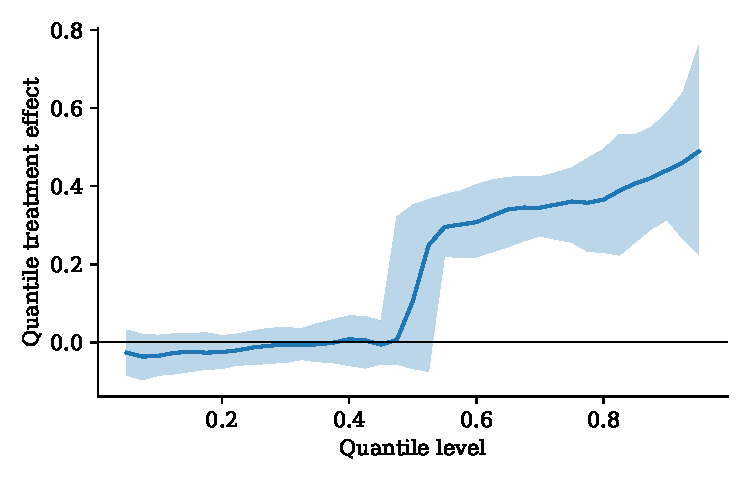
\includegraphics[width=\linewidth]{qte.pdf}
\caption{Posterior mean and 95\% band, from 400 Bayesian bootstrap draws, of the quantile treatment effect in a simulated randomized trial in which only units above the control median benefit.}
\label{fig:qte}
\end{figure}

The Bayesian bootstrap is the simplest generative posterior: each draw reweights the observed units by Dirichlet weights and computes every functional on the reweighted law. In a randomized trial without covariates it is the limit of the Dirichlet process posterior as the concentration parameter tends to zero (Exercise~\ref{ex:ch08:5}). With covariates, GenTE replaces it with a learned conditional map.

\section{Uncertainty for a learned map}

Stochastic gradient descent gives a point estimate of $G$. Three routes supply uncertainty\index{GenTE!uncertainty for a learned map|textbf}.

\paragraph{Bayesian bootstrap of the training data.} Retrain the network on Dirichlet reweighted data, one full training run per draw. This approximates a posterior under a nonparametric prior. The 401(k) analysis of Section~\ref{sec:deephd} uses 200 fits for bands on average, quantile and subgroup effects.

\paragraph{Deep ensembles.} Train networks from different initializations\index{deep ensemble|textbf}. Their spread captures sensitivity to the optimizer's starting point, but has no direct Bayesian justification or posterior interpretation.

\paragraph{Generative Bayesian computation.} Learn a second map, from noise and a summary of the data to a low dimensional parameter such as the average effect, trained on data sets simulated from the prior and the model and amortized over them (Chapter~\ref{ch:computation}).

In practice we use the bootstrap for final reporting and generative Bayesian computation for exploration. The bootstrap measures sampling variability given the architecture; the ensemble measures training variability. Neither covers architecture error: in the 401(k) analysis, 200 irrelevant covariates, fed directly to the network, move the quantile effect curve without widening its bands (Section~\ref{sec:deephd}). Before reporting a band on real data, simulate from a truth resembling the data, refit, and check how often it covers the truth (Section~\ref{comp:sec:checks}).

\section{Deep learning for high dimensional inference}\label{sec:deephd}

Every object of Bayesian causal inference, a posterior, a conditional outcome law, a potential outcome, is a conditional distribution, and so by noise outsourcing a function of uniform noise and the conditioning variables. Deep networks are the standard tool for learning functions of many inputs. Put the two together and high dimensional inference\index{deep learning for high dimensional inference|textbf} becomes supervised learning: the curse of dimensionality moves from integration, where Markov chain Monte Carlo suffers, to regression, where networks are strong.

\paragraph{Generative causal inference.} Nareklishvili, Polson and Sokolov (2023a) learn a posterior map from uniform noise and a data summary $S(D)$, without evaluating a likelihood or estimating a density (Chapter~\ref{ch:computation}). Models with deterministic latent updates need only a simulator; accuracy rests on the summary and network. Here the outcome map is fitted to a fixed observed data set rather than amortized over prior simulations.

\paragraph{Deep partial least squares.} With many covariates or instruments, Nareklishvili, Polson and Sokolov (2023b) first project them onto a few partial least squares\index{deep partial least squares|textbf} directions, chosen for their covariance with the outcome, and then fit a deep network to the scores. A result of Brillinger (2012) explains why this works: with Gaussian regressors, the least squares direction is proportional to the index of a single index model for any link correlated with that index, and the first partial least squares direction to the covariance matrix of the regressors times the index, the same direction when that matrix is spherical. When the retained directions span the index, the projection keeps the signal and the network learns the nonlinearity in a few dimensions. The paper applies it to the Angrist and Evans (1998) data on childbearing and mothers' labour supply, with sparse and correlated instruments.

\paragraph{Feature selection for personalized policy.} Forest PLS (Nareklishvili, Polson and Sokolov 2023c) uses the same projection to select the covariate directions along which effects vary, and fits causal forests within them, with consistency and asymptotic normality for the personalized effects. In the Pennsylvania reemployment bonus experiments it found that cash incentives drew some young nonwhite participants into work while cushioning others from searching, a heterogeneity an average effect hides.



\paragraph{How the pieces fit.} The pipeline is: reduce dimension along directions that predict both outcome and treatment, by projection or a learned embedding; learn the conditional law with a quantile network; obtain uncertainty by training on prior simulations, which gives a posterior, or by refitting under Dirichlet weights, the weighted Bayesian bootstrap of Newton, Polson and Xu (2021); and read off effects as accountings. A network does not remove confounding: a projection chosen only for the outcome can discard the covariates that drive treatment, as the remark on the propensity network explains.

\subsection{A high dimensional distributional analysis of 401(k) eligibility}

We fit the pipeline to the 1991 SIPP data of Chapter~\ref{ch:k401}: 9{,}915 households, eligibility for a 401(k) plan\index{401(k) plan!high dimensional distributional analysis|textbf} as treatment, net financial assets in thousands of dollars as outcome, and the nine standard covariates (age, income, education, family size, marital status, two earner status, defined benefit pension, IRA participation and home ownership). A single quantile network, with eligibility as one of its inputs and without GenTE's propensity and effect heads, learns the conditional law of assets given covariates and eligibility. The level $u$ enters through a cosine embedding with 32 terms, the covariates and eligibility $(x, t)$ through two ReLU layers of width 64, and the two are multiplied coordinatewise before a two layer head that returns the quantile. This is the architecture of Figure~\ref{fig:qnnarch}, with $(x, t)$ in the place of the summary. Training minimizes the weighted check loss at four random levels per observation for 40 epochs. We refit it 200 times under independent exponential weights (normalized, these are Dirichlet weights), so that each fit is one draw from the weighted Bayesian bootstrap, and for each draw simulate both potential outcomes for every household. Every generative estimate below comes from those 200 fits, and each network in the experiment with 200 added covariates is refitted 200 times in the same way.

\paragraph{The average effect.} The posterior mean of the average effect is 8.87 thousand dollars, with 95\% interval $[7.54, 10.20]$, the mean of the 200 refits plus or minus 1.96 standard deviations.

The DML estimates of Table~\ref{tab:k401} are 9.52, $[6.89, 12.14]$, with lasso nuisances and 8.59, $[6.05, 11.12]$, with forests, with intervals about twice as wide. The DML rows come from one random partition of the data and use the partially linear score, which with varying effects estimates the average of $\tau(x)$ weighted by $e(x)\{1 - e(x)\}$. The generative 8.87 averages the household effects without weights. DML with the interactive score, which estimates that unweighted average, gives 8.17, $[5.74, 10.59]$, with lasso nuisances and 7.74, $[5.37, 10.11]$, with forests on the same partition, and the medians over 20 and 5 partitions are 8.40 and 8.05. The forest puts the propensity of 41 to 56 households, depending on the partition, below 0.01 or above 0.99, and clipping it at 0.01 and 0.99 leaves them weights of up to 100. Both estimates lie below the generative one but within one of their standard errors of it, and their intervals are again about twice as wide. The lasso median sits 0.47 below 8.87, close to the upward bias of 0.44 that the coverage check below finds in the refits on simulated data.

The bootstrap interval reflects sampling variability given the network; it does not include uncertainty about the architecture, and in the coverage check after Figure~\ref{fig:deepcate} it covers 92 percent rather than 95. Nor is all of its width sampling variability. When 20 fixed sets of weights are each refitted under three training seeds, the seed accounts for 14 percent of the variance of the average effect across refits (a standard deviation of 0.22 against 0.53 from the weights) and for 46 percent of the variance of a quantile effect, averaged over the 19 levels (20 to 84 percent).

\paragraph{Every quantile.} Figure~\ref{fig:deepqte} shows the quantile treatment effects. They are between 1.1 and 1.7 thousand dollars up to the 30th percentile, 3.72 at the median, 12.87 at the upper quartile and 23.93 at the 90th percentile. The classical inverse propensity weighted quantiles of Firpo (2007) are 1.01, 0.87, 5.03 and 13.46 at the 10th, 25th, 50th and 75th percentiles. Their propensity score is a logistic regression of eligibility on the nine covariates, linear in them and fitted once, and their bands come from 200 Bayesian bootstrap draws. They track the generative curve up to about the 80th percentile except around the median, where they run higher and the two bands do not overlap; they then flatten to 15.59 at the 90th, with a wide band. In the upper tail the weighted estimator rests on a few heavily weighted households, while the generative model borrows strength across covariates; the two disagree most where the data are thinnest, and the model's answer there leans on its extrapolation.

\begin{figure}[ht]
\centering
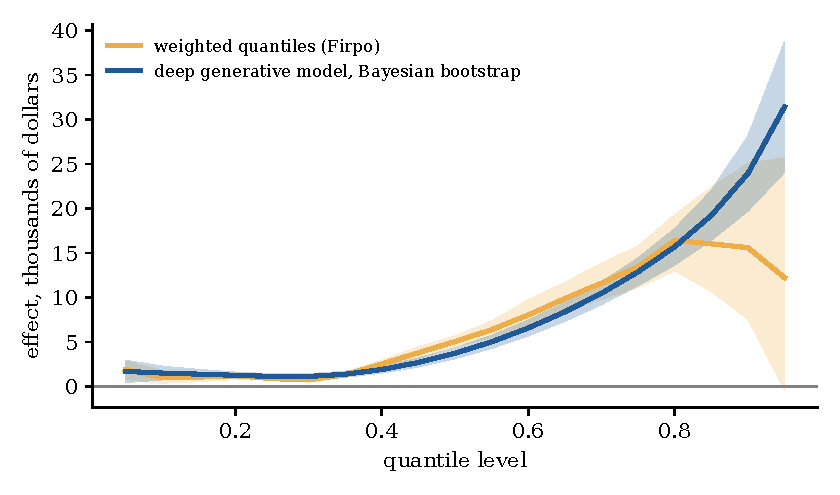
\includegraphics[width=0.92\linewidth]{deep401k_qte.pdf}
\caption{Quantile treatment effects of 401(k) eligibility on net financial assets: the deep generative model with 200 weighted Bayesian bootstrap fits, and the inverse propensity weighted quantiles of Firpo with 200 Bayesian bootstrap draws. Bands are nominal 95\% intervals: for the generative model the mean of the 200 fits plus or minus 1.96 standard deviations, for Firpo's estimator the 2.5 and 97.5 percent points of the 200 draws. The text checks the coverage of the first.}
\label{fig:deepqte}
\end{figure}

\paragraph{Every subgroup.} The same draws give conditional effects for any subgroup at no extra cost. Figure~\ref{fig:deepcate} shows them by income quintile and by age. The effect rises steadily with income, from 3.11 thousand dollars in the lowest quintile to 18.15 in the highest, with intervals $[2.30, 3.91]$ and $[14.20, 22.11]$, and with age, from 4.87 for households headed by someone under 36 to 14.73 for those over 55. Eligibility matters most for households that have the income to save and the years of saving behind them.

\begin{figure}[ht]
\centering
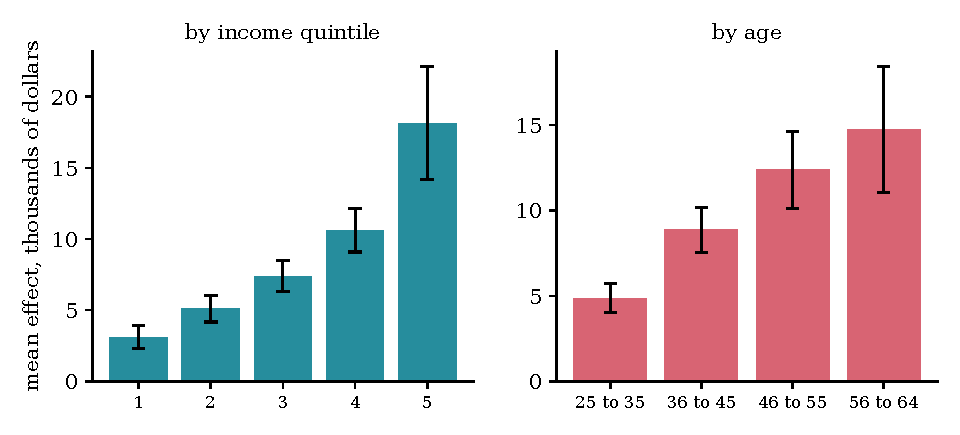
\includegraphics[width=\linewidth]{deep401k_cate.pdf}
\caption{Mean effect of 401(k) eligibility by income quintile and by age of the household head, with nominal 95\% weighted Bayesian bootstrap intervals, the mean of the 200 refits plus or minus 1.96 standard deviations.}
\label{fig:deepcate}
\end{figure}

\paragraph{Coverage of the bands.} The check of Section~\ref{comp:sec:checks} needs a known truth, so we built one that resembles these data. One network, fitted to them once with unit weights and the same training, serves as the true conditional law. Each of 1,000 simulated data sets keeps the 9,915 households' covariates and eligibility and draws their assets from that law, so unconfoundedness holds and every effect is known; the true average effect is 8.49. Each data set was then analysed as the real one, with 200 refits under Bayesian bootstrap weights and the band printed in this section, the mean of the refits plus or minus 1.96 standard deviations, and again with only its first twenty refits. The bands covered the truth in these percentages of the data sets:
\begin{center}
\begin{tabular}{lcc}
\toprule
Target & 20 refits & 200 refits \\
\midrule
Average effect & 90 & 92 \\
Quantile effects, mean over 19 levels & 92 & 94 \\
Income quintile effects & 85 to 93 & 89 to 95 \\
\bottomrule
\end{tabular}
\end{center}
The Monte Carlo standard error of the 92 is 0.8 points. Quantile coverage is pointwise, at the levels 0.05 to 0.95; with 200 refits it is lowest at the 15th percentile, 84 percent, and 90 percent at the 95th. A calibrated band of this form built from 200 draws would cover about 95 percent. Most of the rest of the shortfall is bias: the refits overstate the average effect by 0.44, two thirds of their standard deviation, every quintile effect by 0.30 to 0.57 and the effect at the 95th percentile by 3.1 thousand dollars. Going from twenty refits to 200 raises coverage by two to four points but leaves the bias of the average effect where it was, 0.44 either way; only a better fitted network would remove it. With twenty refits the other natural band, the 2.5 and 97.5 percent points of the refits, lies close to the smallest and largest draws and covers only 82 percent for the average effect, which is why we print the wider one; with 200 the two nearly agree (91 and 92 percent).

\paragraph{A truth outside the network family.} The truth of the check above comes from the model's own family, the most favourable case. We repeated the check on 200 data sets drawn from a truth outside it, keeping the households' covariates and eligibility. With $x_1, \ldots, x_4$ the standardized age, income, education and family size, the outcome under treatment $t$ was
\[
Y(t) = 3x_1 + 2\sin x_2 + x_3x_4 + t\{2 + 2\,\mathbf{1}(x_2 > 0)\} + (1 + 0.5|x_1|)(1 + 0.5t)\,\varepsilon,
\]
\[
\varepsilon = \frac{e^{Z} - e^{1/2}}{\sqrt{e(e - 1)}}, \qquad Z \sim N(0, 1),
\]
a nonlinear mean, an effect of 2 below mean income and 4 above it, and skewed heteroskedastic noise with mean zero and variance one, drawn independently for each household and data set. The true average and income quintile effects follow from the effect function, and the true quantile effects were computed from 1,000 noise draws per household. Each data set was analysed with 200 refits, as before. There the nine covariate band covered the average effect in 29 of the 200 data sets (34 with twenty refits): its bias of $-0.10$ on an effect of 2.80 is small, but nearly three times the spread of the refits. It covered the quantile effects in 75 percent on average and missed the effect in three of the five income quintiles in every data set.

\paragraph{Two hundred irrelevant covariates.} To see what high dimensions do, we appended 200 independent standard normal covariates, so that 209 inputs carry the information of nine. A network fed all 209 inputs gives an average effect of 7.76, $[6.29, 9.22]$, and its quantile effect curve lies at a root mean squared distance of 1.48 from the nine covariate curve. Projecting the 209 inputs onto five partial least squares directions that predict both assets and eligibility puts 73.5\% of the squared weight on the nine real covariates, which are 4.3\% of the inputs. The network on those five scores gives 8.39, $[6.94, 9.84]$, at a distance of 1.08 (Figure~\ref{fig:deephd}). The projection helps, but neither version recovers the nine covariate answer exactly. Each network was refitted 200 times, as the nine covariate fit was. The average band width, the width of the 95\% band averaged over the 19 levels, is 2.89 for the nine covariate fit, 2.74 for the raw network and 3.05 for the projected one. The raw network, the farther of the two from the nine covariate answer, reports the narrower band. The fits use the same households, so the distance between them measures how much the answer depends on the inputs and the architecture, though not which fit is nearer the truth, and a bootstrap over one architecture does not see it. The projected network's band is wider at most levels and most of all at the top, where its 200 refits put the effect at the 0.95 quantile anywhere from 18 to 39 thousand dollars. 

We ran the high dimensional check on the first 200 of the 1,000 data sets generated from the fitted network, each with 200 fresh noise covariates, and 20 refits per fit. The projected network had its directions either fitted once per data set or refitted with the weights in every refit. Coverage, in percent of the data sets, was
\begin{center}
\small
\begin{tabular}{lccc}
\toprule
Inputs & Average & Quantile & Lowest income \\
 & effect & effects & quintile \\
\midrule
Nine covariates & 90.5 & 91.8 & 83.5 \\
All 209 inputs & 85.0 & 68.3 & 88.0 \\
Five PLS scores, directions fixed & 92.5 & 84.5 & 51.0 \\
Five PLS scores, directions refitted & 90.0 & 81.6 & 39.5 \\
\bottomrule
\end{tabular}
\end{center}
with the quantile column averaged over the 19 levels. The raw network understates the average effect by 0.46, covers the quantile effect at its worst level in 3.5 percent of the data sets, and covers the second and third income quintiles in about half. A hundred refits on 20 of the data sets left the coverage of the quantile effects where it was. The raw network's band, the narrowest of the three, is the one that covers least.

\begin{figure}[ht]
\centering
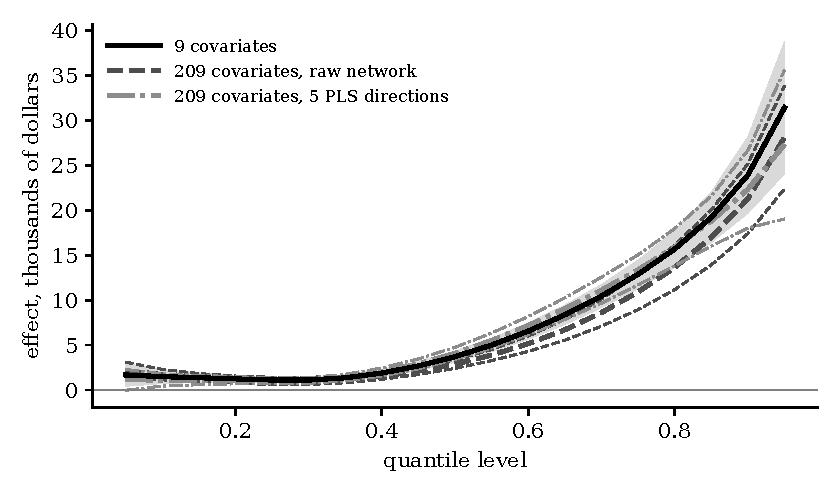
\includegraphics[width=0.92\linewidth]{deep401k_hd.pdf}
\caption{Quantile treatment effects with the nine covariates, with 200 added irrelevant covariates fed directly to the network, and with the 209 covariates projected onto five partial least squares directions. Bands are nominal 95\% weighted Bayesian bootstrap intervals, the mean plus or minus 1.96 standard deviations of 200 refits each, in gray fill for the nine covariate fit and as thin lines in the style of their curves for the other two.}
\label{fig:deephd}
\end{figure}

\section{Individualized decisions}

The conditional laws support decisions\index{individualized decisions|textbf} that averages cannot. If treatment costs $k$ and outcome $y$ has utility $\mathcal{U}(y)$, treating a unit with covariates $x$ is optimal when
\[
\int \mathcal{U}(y)\,dF_1(y \mid x) - \int \mathcal{U}(y)\,dF_0(y \mid x) > k.
\]
When $\mathcal{U}$ is linear this depends only on $\tau(x)$. When $\mathcal{U}$ is concave, as usual for health or income, it depends on the whole conditional law, particularly the lower tail. A risk averse policymaker wants to know whether treatment protects against bad outcomes, a statement about lower quantiles, which GenTE supplies.

In the simulated trial of Figure~\ref{fig:qte}, a linear utility and $\tau(x) > k$ would treat everyone, and for half of them the cost $k$ buys nothing. A concave utility weights the unaffected lower half more heavily, and the quantile effect curve, flat up to the median, shows at once where the gain is absent, if ranks are preserved (Section~\ref{sec:ot}). In quantile form the expected utility\index{expected utility|textbf} rule is
\[
\int_0^1 \bigl[\mathcal{U}\{q_1(u \mid x)\} - \mathcal{U}\{q_0(u \mid x)\}\bigr]\,du > k,
\]
computed from the fitted map by averaging over draws of $u$.

Report both conditional quantile functions, or the baseline $q_0(u \mid x)$ and difference $\Delta(u \mid x)$. The difference alone suffices for linear utility; concave utility needs the level as well as the change. For any specified utility and cost, the posterior of the expected utility difference shows how confident the recommendation to treat is for a unit at $x$. Changing the utility needs no refit.

\paragraph{Dominance.} At zero cost and fixed $x$, with finite means, treatment is at least as good for every increasing utility if and only if $F_1(y \mid x) \leq F_0(y \mid x)$ for every $y$ (first order dominance), equivalently $q_1(u \mid x) \geq q_0(u \mid x)$ for every $u$. It is at least as good for every increasing concave utility if and only if $\int_0^u q_1(v \mid x)\,dv \geq \int_0^u q_0(v \mid x)\,dv$ for every $u \in (0, 1]$ (second order dominance), a statement about the lower tail that does not require choosing $\mathcal{U}$ (Shaked and Shanthikumar 2007). Both compare marginal laws and need no coupling. Neither identifies the fraction of units helped, which the marginals bound but do not determine (Section~\ref{sec:ot}). The posterior probability of the inequality over the whole curve is computed draw by draw; pointwise bands on the quantile effect do not establish it.

\section{Heterogeneity and the horseshoe}

Shrinkage matters most for heterogeneity\index{heterogeneous treatment effects!and the horseshoe|textbf}. With $p$ covariates there are $p$ potential effect modifiers, most doing nothing. Writing $\tau(x) = \tau_0 + \sum_j \delta_j x_j$ with a horseshoe on $\delta_j$ gives a posterior that shrinks the many small modifiers toward zero and, through its heavy tails, leaves a strong modifier nearly unshrunk; a moderate modifier is still shrunk, as Chapter~\ref{ch:horseshoe} finds for confounders.

The Bayesian causal forest\index{Bayesian causal forest} takes a related route with tree ensembles: a baseline forest $\mu_0(x)$ with the propensity as input, and a separate, more strongly regularized forest for $\tau(x)$, which encodes the judgement that effects vary less than outcomes. GenTE encodes it through its separate $\Delta$ head.

The common thread is that heterogeneity is a sparse signal on top of a dense one. Outcomes depend on many covariates; the effect, in most applications, depends on a few, and a learner that treats the two symmetrically, fitting a treated surface and a control surface and subtracting, spends its capacity on the baseline and reports the noise of that subtraction as heterogeneity. The 401(k) analysis of Section~\ref{sec:deephd} uses a single quantile network with eligibility as an input, so it does not test this design, but it does show an effect of eligibility that moves with income and age.

Report the posterior of each modifier: a horseshoe posterior that leaves $\delta_j$ near zero is a finding about covariate $j$, not a failure to find one.

\section{Quantile regression as a likelihood}

The check loss\index{check loss!as a likelihood|textbf} training GenTE's quantile heads\index{quantile regression|textbf} has a Bayesian reading. Yu and Moyeed observed in 2001 that minimizing $\sum_i \rho_u(y_i - q(x_i))$ is equivalent to maximizing the likelihood of an asymmetric Laplace distribution\index{quantile regression!asymmetric Laplace likelihood|textbf} with location $q(x)$:
\[
f_u(y \mid q) = u(1 - u)\exp\{-\rho_u(y - q)\}.
\]
The check loss identifies the true conditional quantile, but the spread of the posterior under this working likelihood is not calibrated, because the asymmetric Laplace is not the true conditional law. Sandwich corrections, or a Bayesian bootstrap\index{Bayesian bootstrap} of the check loss, aim to restore calibration. 

The reading also clarifies what the network is doing. Minimizing the check loss at a randomly drawn level $u$ on every pass is, in expectation over $u$, maximizing a product of asymmetric Laplace likelihoods across all levels at once, and because the levels share one set of weights, the network is a joint model of the whole conditional law and not a collection of separate quantile regressions. The product is a working criterion, not the likelihood of one outcome; integrated over $u$, the same loss of a curve that increases in $u$ is half the continuous ranked probability score of the law the curve describes (Section~\ref{comp:sec:network}), a proper score for the whole distribution.

Joint training shares information across quantile levels but does not prevent crossing. A monotone head, such as a cumulative sum of positive increments over a grid of $u$, rules out crossing by construction.

\section{The Stefan Boltzmann application}

The Stefan Boltzmann law states that the luminosity of a star is $L = 4\pi R^2\kappa T^4$, where $R$ is its radius, $T$ its surface temperature and $\kappa$ the Stefan Boltzmann constant. Temperature causes luminosity, and the law makes sharp predictions: the effect must be positive for every star and, for a given temperature contrast, scale with the emitting area $R^2$, so it should vary over orders of magnitude across stars of different sizes.

The GenTE paper\index{GenTE!Stefan Boltzmann application|textbf} uses a public catalogue of 240 stars, 40 in each of six classes from brown dwarfs to hypergiants. Treatment is being hotter than the median temperature, the outcome is luminosity, and the covariates are radius and, in one specification, stellar colour and class. The example teaches an overlap lesson. Colour is nearly a deterministic function of temperature, and three of the six classes lie entirely on one side of the median, so with colour and class as covariates the propensity is zero or one for almost every star. The generalized random forest then returned negative effects for every star, with a median of about $-7.6 \times 10^4$ solar luminosities, a sign the law forbids; GenTE's stayed positive, but where overlap fails neither method estimates anything, only extrapolates. With radius alone, which varies within both temperature groups, both recovered the correct sign, and GenTE's estimates spanned five and a half orders of magnitude, ordered by stellar size, dwarfs smallest and supergiants and hypergiants largest, as the $R^2$ factor requires.

 A physical law also gives an external standard no simulation can provide: the estimates lie where the law says they must.

\section{Comparison with conformal prediction}

Conformal methods\index{conformal prediction|textbf} give distribution free prediction intervals for individual outcomes, extended to individual treatment effects\index{individual treatment effect|textbf} by Lei and Cand\`es (2021), with marginal coverage under exchangeability\index{exchangeability} and no outcome model, given the propensity score. Their weakness is the converse of their strength: coverage is marginal over covariates, so an interval can have the right average coverage while undercovering some subgroups and overcovering others.

The generative approach reports the conditional law itself, giving intervals for the outcome under either treatment at any covariate value, with coverage that depends on the model being adequate. The two are complementary: conformal calibration can check the generative model's intervals, and a failed check means the model needs work. But how the effect varies across people comes from the model, and a conformal interval around a poor model is valid on average and too wide to help.

A posterior band and a conformal interval cover different objects, so their widths cannot be compared. The nominal 95\% band $[2.30, 3.91]$ thousand dollars for the lowest income quintile in the 401(k) analysis (Section~\ref{sec:deephd}) covers a mean effect and shrinks as the sample grows. A conformal interval for one household's effect must also cover the spread of individual effects among similar households, with validity averaged over households. That spread depends on the conditional covariance of $Y(1)$ and $Y(0)$, unidentified without a coupling (Section~\ref{sec:ot}). The conditional laws do determine outcome intervals for $Y(t)$ at a given $x$, which a conformal check can test.

Use conformal checks as a diagnostic and the generative model as the report. Split off a calibration set and compute coverage of the model's outcome intervals within each arm and a few subgroups that matter for the decision, with binomial standard errors. If coverage is far from nominal, revise the model. This cheap check uses the learner's own intervals and assumes only independent draws from the training population. It tests the laws of $Y$ given $X = x$ and $T = t$, which equal those of $Y(t)$ given $X = x$ only under ignorability and overlap; it cannot test those assumptions.

\section{Policy learning}

Given the posterior of the conditional laws, the optimal policy of Chapter~\ref{ch:predictive} can be computed directly. The frequentist alternative, empirical welfare maximization\index{empirical welfare maximization|textbf}\index{EWM|see{empirical welfare maximization}}, chooses a policy from a restricted class to maximize a doubly robust estimate of welfare, as in Athey and Wager's (2021) work on policy learning\index{policy learning|textbf}, with regret\index{regret} bounds relative to the best policy in the class.

The Bayesian policy maximizes posterior expected welfare within the permitted class, say simple rules clinicians can apply. The model first approach separates the scientific step, learning how outcomes depend on covariates and treatment, from the decision step, and lets each be done properly.

Empirical welfare maximization cross fits its nuisances once, so a new policy class or a cost per treated unit reuses the same doubly robust scores; a utility not linear in the outcome, or a target such as a quantile or the lower tail, needs a new score and a new outcome regression, of $\mathcal{U}(Y)$ or of $\mathbf{1}(Y \leq y)$ on the covariates, unless the nuisance fitted is the whole conditional law. The Bayesian analyst fits the conditional laws once and evaluates any policy, cost and utility against the same posterior draws. In the 401(k) analysis of Section~\ref{sec:deephd}, a program that targets eligibility by income and one that targets it by age can both be read from the same 200 fits, and their posterior welfare compared directly, concave utilities included.

Two rules whose posterior welfare difference, computed draw by draw, puts substantial mass on both sides of zero are not distinguished by the data, and a regret bound for the better one does not change that. We regard the comparison of posterior welfare across candidate rules, and not the optimality of the maximizer, as the output a decision maker should see.

\section{Optimal transport and joint potential outcomes}\chlabel{ch:ot}\label{sec:ot}

So far this chapter has concerned the marginal laws $F_0$ and $F_1$ of the potential outcomes. The fraction helped, the fraction harmed and the distribution of individual gains depend on their joint law\index{potential outcomes!joint law of|textbf}, a never observed coupling that the marginals bound without identifying, and whose posterior does not concentrate.

Practitioners ask these questions most naturally and answer them most carelessly. A quantile treatment effect that is positive at every $u$ is routinely read as saying that everyone gains, and a zero average effect as saying that treatment does nothing, and neither reading follows from the marginals. Optimal transport\index{optimal transport|textbf} defines a canonical coupling, and a prior covers the rest.

\subsection{The coupling problem}

Suppose the marginals $F_0$ and $F_1$ are known exactly, as from an infinitely large randomized trial. The joint law $H$ of $(Y(0), Y(1))$\index{coupling!of potential outcomes|textbf} can be any law with these marginals\index{coupling|textbf}. By Sklar's theorem\index{Sklar theorem@Sklar's theorem},
\[
H(y_0, y_1) = C\{F_0(y_0), F_1(y_1)\}
\]
for some copula\index{copula|textbf} $C$, and every copula is possible. The data say nothing about $C$.

\begin{theorem}[Fr\'echet and Hoeffding]
Every copula satisfies
\[
\max(u + v - 1, 0) \leq C(u, v) \leq \min(u, v).
\]
The upper bound\index{Frechet Hoeffding bounds@Fr\'echet Hoeffding bounds} is the comonotone copula, under which $Y(1) = F_1^{-1}\{F_0(Y(0))\}$ when $F_0$ is continuous; the lower bound is the countermonotone copula.
\end{theorem}

The comonotone coupling\index{coupling!comonotone and countermonotone|textbf} is rank preservation\index{rank preservation|textbf}: a unit at the $u$ quantile under control stays there under treatment, so its individual effect equals the quantile treatment effect\index{quantile treatment effect} at that level. For a group action, Theorem~\ref{gr:thm:recon} makes every unit's effect the group effect on the chart scale. Rank preservation is often implicit and rarely defended. The countermonotone coupling sends the best off under control to the worst off under treatment. Though rarely plausible, it is as consistent with the data as any other copula.

\paragraph{Bounds on the distribution of gains.} Let $\eta = Y(1) - Y(0)$ be the individual gain\index{individual gain|textbf}. Its distribution function $F_\eta$ is not identified, but it is bounded.

\begin{theorem}[Makarov]
For every $\delta$,
\begin{align*}
F_\eta(\delta) &\geq \sup_y \max\{F_1(y) - F_0(y - \delta), 0\},\\
F_\eta(\delta) &\leq 1 + \inf_y \min\{F_1(y) - F_0(y - \delta), 0\},
\end{align*}
and, when $F_0$ and $F_1$ are continuous, the bounds\index{Makarov bounds|textbf} are pointwise sharp: each is the infimum or supremum of $F_\eta(\delta)$ over the joint laws with these margins.
\end{theorem}

Figure~\ref{fig:makarov} shows the bounds\index{fraction helped!bounds on|textbf} on $\Prob\{Y(1) > Y(0)\}$, the fraction helped\index{fraction helped|textbf}, when both marginals are normal with unit variance and the treated marginal is shifted by $s$. Even with a shift of one standard deviation, the fraction helped can be anywhere from about 0.38 to 1: 0.76 under independence, 1 under rank preservation, and only 0.69 under the countermonotone coupling, so the extreme copula does not give the extreme fraction helped. No amount of data can choose among these. An analyst who reports the fraction helped from a trial, without saying which coupling she assumed, has reported a number that could be replaced by any other in that interval on the same evidence.

\paragraph{Covariates sharpen the bounds.} With identified conditional laws that are continuous for $Q$ almost every $x$, the coupling can be chosen separately at each $x$, so the sharp bounds on $F_\eta(\delta)$ are the conditional Makarov bounds, computed from $F_0(\cdot \mid x)$ and $F_1(\cdot \mid x)$ and then averaged over $Q(dx)$ (Makarov 1981; Kallus 2022). The result is never looser than the unconditional bounds. Let $X$ be 0 or 1 with probability one half, the control outcome uniform on $(10x, 10x + 0.1)$ and the treated outcome uniform on $(10x + 1, 10x + 1.1)$. Given $x$, every unit is helped. From the unconditional marginals alone the fraction helped can be anywhere from one half to one. In a posterior analysis the conditional bounds are computed within each draw of the conditional laws, so the band on each endpoint is distinct from the width of the identified interval. Chapter~\ref{ch:tianpearl} gives the binary case.

\begin{figure}[ht]
\centering
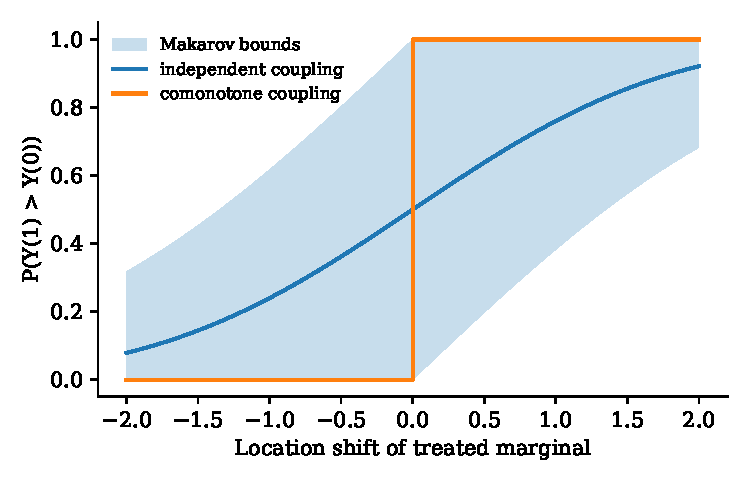
\includegraphics[width=\linewidth]{makarov.pdf}
\caption{Bounds on the fraction helped by treatment, with standard normal control outcomes and treated outcomes shifted by the amount on the horizontal axis. Independent and comonotone couplings are shown for comparison.}
\label{fig:makarov}
\end{figure}

\subsection{Optimal transport}

Optimal transport gives a principled way to pick a coupling, or a family of them, when one must. Given a cost $c(y_0, y_1)$, the Kantorovich problem is
\[
\min_{H \in \Pi(F_0, F_1)} \int c(y_0, y_1)\,dH(y_0, y_1),
\]
over all couplings $H$ with the given marginals.

\begin{proposition}
For real valued outcomes with finite means and any cost $c(y_0, y_1) = h(y_1 - y_0)$ with $h$ convex, the comonotone coupling is optimal.
\end{proposition}

\begin{proof}
For convex $h$ the cost is submodular, and for submodular costs on the real line the monotone rearrangement is optimal. This is the classical result on monotone transport; see Villani (2009), and Exercise~\ref{ex:ch09:4} for a two point exchange argument.
\end{proof}

Rank preservation\index{rank preservation} minimizes the average convex cost of individual gains. Optimal transport\index{optimal transport} thus gives a canonical coupling, but no causal justification for it. The analyst must say whether she believes it.



\subsection{A Bayesian treatment of the coupling}

The Bayesian response to an unidentified parameter is to put a prior on it. For the coupling, a Gaussian copula\index{copula!Gaussian|textbf} with correlation $\rho$ is convenient:
\[
C_\rho(u, v) = \Phi_2\{\Phi^{-1}(u), \Phi^{-1}(v); \rho\}.
\]
Then $\rho = 1$ is rank preservation, $\rho = 0$ is independence, and $\rho = -1$ is the countermonotone coupling.

The full posterior is $\pi(F_0, F_1, \rho \mid \text{data}) = \pi(F_0, F_1 \mid \text{data})\,\pi(\rho)$, since the data do not inform $\rho$ and the prior takes $\rho$ independent of $(F_0, F_1)$. A functional such as the fraction helped\index{fraction helped!posterior of|textbf} is computed draw by draw: for each draw of the marginals and $\rho$, compute $\Prob\{Y(1) > Y(0)\}$. Its posterior spread has a part from the marginals, which shrinks with $n$, and a part from $\rho$, which does not.

\begin{proposition}
Suppose $\rho$ is a priori independent of $(F_0, F_1)$, the likelihood depends on $(F_0, F_1)$ alone, the posterior of $(F_0, F_1)$ is consistent at the true marginals, and $\psi$ is continuous in $(F_0, F_1)$ for each $\rho$. As $n \to \infty$, the posterior of $\psi(F_0, F_1, \rho)$ converges weakly to the law of $\psi(F_0^*, F_1^*, \rho)$ with $\rho$ drawn from its prior, where $F_t^*$ are the true marginals.
\end{proposition}

This is Proposition~\ref{prop:partial} of Chapter~\ref{ch:tianpearl} with $\phi = (F_0, F_1)$ and $\xi = \rho$; Appendix~\ref{app:theory} gives the proof. A reader who disagrees can substitute her own prior and see at once how the answer changes.

Take the setting of Figure~\ref{fig:makarov}: both marginals normal with unit variance, the treated one shifted by $s$, and a Gaussian copula. The gain $Y(1) - Y(0)$ is then normal with mean $s$ and variance $2 - 2\rho$, so the fraction helped is $\Phi\{s/\sqrt{2 - 2\rho}\}$. At $s = 1$, a uniform prior on $\rho \in [0, 1]$ gives a limiting posterior on $[0.76, 1]$ with median 0.84, and more data cannot narrow it. Even $\rho = -1$ gives only 0.69, against the Makarov lower bound of 0.38, so the Gaussian copula family is itself a restriction that the prior imposes.

\paragraph{Where prior information about the coupling comes from.} The copula is not identified from a single experiment, but it is not beyond knowledge. In a crossover trial, units are observed under both treatments at different times, partly revealing the joint law under assumptions about carryover and time trends. In Student's (1931) twin design, one twin's control outcome informs the other's because identical twins share most determinants of $Y(0)$; within pair correlation constrains $\rho$. Earlier crossover or twin studies in the same field can supply strong priors on $\rho$. Rank preservation\index{rank preservation} is plausible if treatment adds a dose depending weakly on individual characteristics; if it switches some units into a different regime, it is not.

\subsection{An empirical consideration}

When panel data span a policy change affecting only some units, persistence among unaffected units can inform the copula\index{copula} prior: if persistence is high, rank preservation is plausible for the treated too, and a prior concentrated near $\rho = 1$ is defensible.

Among unaffected units, compute the Spearman correlation $r_S$ of pre and post outcomes. Under a Gaussian copula, $\rho = 2\sin(\pi r_S/6)$ estimates rank persistence; its sampling uncertainty gives the prior width. Centre the prior there and widen it to allow treatment to disturb ranks more than time alone. For each posterior draw of the marginals and $\rho$, compute the fraction helped, fraction harmed\index{fraction harmed|textbf} and gain quantiles. Report these alongside the same functionals under rank preservation and independence, so the reader sees how much the prior supplies.

Persistence among unaffected units concerns $Y(0)$ over time, so it informs $\rho$ without measuring the relation between $Y(0)$ and $Y(1)$. Treatment can break ranks that time preserves. At $\rho = 1$, each unit's gain equals the quantile effect at its rank (Exercise~\ref{ex:ch09:2}); concentrating a prior near that point nearly asserts the same and should be reported as such.

\subsection{Brenier's theorem and multivariate outcomes}

For real outcomes the monotone rearrangement solves every convex transport problem; for vector outcomes the analogue is Brenier's theorem\index{Brenier theorem@Brenier's theorem|textbf}.

\begin{theorem}[Brenier]
Let $\mu$ and $\nu$ be probability measures on $\R^d$ with finite second moments, and suppose $\mu$ is absolutely continuous. Then there is a convex function $\varphi$ whose gradient, unique $\mu$ almost everywhere, pushes $\mu$ forward to $\nu$, and the coupling $(X, \nabla\varphi(X))$ with $X \sim \mu$ is the unique optimal coupling for the squared Euclidean cost.
\end{theorem}

The gradient of a convex function generalizes a monotone map. For multivariate potential outcomes, such as blood pressure and cholesterol under a drug, Brenier's map couples each patient's untreated and treated vectors so as to move patients least in aggregate. Chernozhukov, Galichon, Hallin and Henry (2017) used this idea to define multivariate quantiles, and the same construction defines multivariate quantile treatment effect\index{quantile treatment effect}s. The caveat of the real valued case carries over unchanged: Brenier's map is the canonical coupling for the squared cost, not the true one, and a multivariate fraction helped computed from it rests on the multivariate form of rank preservation.

\paragraph{Conditional transport and causal maps.} With covariates, a causal map is a family $\{T_x\}$ with $T_x$ pushing $F_0(\cdot \mid x)$ to $F_1(\cdot \mid x)$. We take $F_0(\cdot \mid x)$ continuous for each $x$ in what follows, so that such a map exists. Under rank preservation\index{rank preservation} conditional on $x$, the individual effect for a unit with covariates $x$ and untreated outcome $y_0$ is $T_x(y_0) - y_0$.

Composing the learned treated quantile function with the untreated distribution function, the inverse of the learned $q_0$, gives the conditional map without another fit. With GenTE's $q_1 = q_0 + \Delta$,
\[
T_x(y_0) = q_1\{F_0(y_0 \mid x) \mid x\} = y_0 + \Delta\{F_0(y_0 \mid x) \mid x\}.
\]
Under rank preservation, then, the individual effect is the effect head evaluated at the unit's own conditional rank. A second route learns $T_x$ as the gradient in $y_0$ of an input convex neural network conditioned on $x$, minimizing transport cost subject to matching the treated conditional law. It enforces Brenier's structure and extends to vector outcomes, where quantile composition is unavailable. Either route inherits uncertainty from the conditional laws; a Bayesian bootstrap gives draws of $T_x$ and every functional of it.

\subsection{Wasserstein effect measures}

Optimal transport also summarizes the difference between treated and untreated laws\index{Wasserstein effect measure|textbf} without choosing a coupling. The $r$ Wasserstein distance\index{Wasserstein distance|textbf}, for $r \geq 1$,
\[
W_r(F_0, F_1) = \Bigl(\int_0^1 |q_1(u) - q_0(u)|^r\,du\Bigr)^{1/r}
\]
for real outcomes, is the size of the smallest individual effects consistent with the two marginals. Depending only on the marginals, it is identified.

\begin{proposition}
For outcomes with finite means and any coupling of $Y(0)$ and $Y(1)$, $\E|Y(1) - Y(0)| \geq W_1(F_0, F_1) \geq |\E Y(1) - \E Y(0)|$.
\end{proposition}

\begin{proof}
The comonotone coupling is optimal for the convex cost $|y_1 - y_0|$ (the proposition above), and its cost is $\int_0^1 |q_1(u) - q_0(u)|\,du = W_1$ (Exercise~\ref{ex:ch09:2}), which gives the first inequality. Jensen's inequality under that coupling gives the second.
\end{proof}

This is an identified lower bound on how much treatment changes people. A treatment with zero average effect but large Wasserstein distance must change some people a great deal, in opposite directions. For real outcomes, $W_1 = \int_0^1 |\Delta(u)|\,du$, the area between the quantile functions. It equals the absolute average effect exactly when $\Delta(u)$ does not change sign. In the 401(k) analysis the curve is positive at every computed level, 0.05 to 0.95, so equality holds unless it changes sign between those levels or in the uncomputed tails. In the simulated trial of Figure~\ref{fig:qte}, the curve is zero below the median and positive above, so $W_1$ equals the average. A sign change, the one case that separates them, is when the average is most misleading.

The identified gap $W_1(F_0, F_1) - |\E\{Y(1) - Y(0)\}|$ bounds $\E|Y(1) - Y(0)| - |\E\{Y(1) - Y(0)\}|$ from below and uses the same posterior draws. The bound can vanish despite large individual changes: if $Y(0)$ is Bernoulli with probability one half and $Y(1) = 1 - Y(0)$, the marginals coincide, $W_1$ and the average effect are zero, and every unit changes by one.

\section{In practice}

\paragraph{The target.} The targets are $\tau(x)$, $\Delta(u \mid x)$, the unconditional quantile effect, and the expected utility difference. Each posterior draw of $G$ gives draws of $q_0$ and $q_1$ at any $(u, x)$: integrating over $u$ gives conditional means, integrating over $x$ with any $Q$ gives marginals, and composing with $\mathcal{U}$ gives expected utilities, all from one fitted model. The fraction helped, the fraction harmed and the distribution of individual gains also depend on the coupling (Section~\ref{sec:ot}) and are computed draw by draw under a prior on it. The posterior mixes a part that concentrates and a part that does not, and the analyst reports both.

\paragraph{What the analyst does differently.} An analyst who wants distributional effects states which functionals of the conditional laws the decision needs, and fits the laws rather than the functionals. She gives the baseline the propensity and keeps the effect as its own component, so that regularization pushes the effect toward homogeneity. She checks overlap before reading any estimate: the generalized random forest gave every star a negative effect when colour and class removed the overlap. She reports bands from refits under Dirichlet weights, says that they condition on the architecture, checks them for coverage on a simulated truth that resembles the data, and checks the model's outcome intervals by conformal coverage in the subgroups that matter. And she reports the quantile curve and the subgroup effects, not the average alone: in the 401(k) data, the average of 8.87 thousand dollars hides effects of 3.11 in the lowest income quintile and 18.15 in the highest.

\paragraph{Against DML.} DML targets a mean, and for a mean it is adequate: with the interactive score, which estimates the same unweighted average as the generative model, the 401(k) estimates are 8.17 and 7.74 against the generative 8.87, each within one standard error of it. DML is also cheaper, since its interval comes from one pass of cross fitting. Quantile effects and lower tail protection under a concave utility are functionals of the conditional laws, and DML with mean nuisances needs a separate score and outcome fit for each (localized DML, Kallus, Mao and Uehara 2024, does this for quantile effects), where the posterior gives them all from the same draws. The fraction helped and the distribution of gains also depend on the coupling, which no method identifies from the marginals; the generative approach can carry a prior on it through the same draws. In the GenTE benchmarks the generative learner had the lowest error for the conditional average effect in 30 of 36 designs. The generative bands do not cover the error of the architecture: on simulated data they covered the quantile effects in only 68 to 85 percent of data sets when 200 irrelevant covariates were among the inputs, and the average effect in 15 percent when the truth lay outside the network family. Two hundred fits also cost more than one.

\section*{Notes}

The GenTE learner, benchmarks and star application are from Nareklishvili, Polson and Sokolov (2025). The earlier work reviewed in Section~\ref{sec:deephd} is their (2023a, 2023b, 2023c); the coupling analysis is their (2026b) working paper. For deep networks with valid inference see Farrell, Liang and Misra (2021). Sources for noise outsourcing, the check loss and the quantile network are in the Notes of Chapter~\ref{ch:computation}.

Quantile treatment effects by inverse propensity weighting are Firpo's (2007), and Chernozhukov, Fern\'andez Val and Melly (2013) treat distributional effects in general as functionals of counterfactual distributions. Chernozhukov and Hansen (2004) estimate quantile effects with an instrument for 401(k) participation. Yu and Moyeed (2001) read the check loss as an asymmetric Laplace likelihood. The Bayesian bootstrap is Rubin's (1981) and its weighted version Newton, Polson and Xu's (2021); for the Dirichlet process behind Exercise~\ref{ex:ch08:5}, see Ferguson (1973).

On the joint law of the potential outcomes, Sklar's theorem and the Fr\'echet and Hoeffding bounds are in Nelsen (2006), the bound on the distribution of gains is Makarov's (1981), and Heckman, Smith and Clements (1997) take up the distribution of gains in programme evaluation.  Brenier's theorem is Brenier (1991), and Chernozhukov, Galichon, Hallin and Henry (2017) turn it into multivariate quantiles. 



\begin{exercises}
\item\label{ex:ch08:3} Explain why the conditional quantile effect $q_1(u \mid x) - q_0(u \mid x)$ is not, in general, the $u$ quantile of the individual effect $Y(1) - Y(0)$ given $x$. Give a two point example.
\item\label{ex:ch08:4} In the simulation of Figure~\ref{fig:qte}, compute the true average effect and compare it with the area under the true quantile effect curve on $(0, 1)$ and with the area of the part of that curve shown in the figure (levels 0.05 to 0.95).
\item\label{ex:ch08:5} Show that, for a base law with a finite mean, the Bayesian bootstrap posterior of a mean is the limit in distribution of the Dirichlet process posterior of the mean as the concentration parameter tends to zero.
\item\label{ex:ch08:6} For a positive outcome and the concave utility $\mathcal{U}(y) = \log y$, with the cost $k$ in utility units, derive the treatment rule in terms of the conditional laws and show that it can differ from the rule $\tau(x) > k$ that linear utility gives.
\item\label{ex:ch08:7} Write a horseshoe model for linear effect modification and derive the Gibbs step for the modifier coefficients $\delta_j$.

\item\label{ex:ch09:1} Verify the Makarov bounds in Figure~\ref{fig:makarov} at $s = 1$ by direct computation.
\item\label{ex:ch09:2} Show that under the comonotone coupling the distribution of gains is the distribution of $F_1^{-1}(U) - F_0^{-1}(U)$, $U$ uniform.
\item\label{ex:ch09:3} For normal marginals with unit variances and a Gaussian copula with correlation $\rho$, compute $\Prob\{Y(1) > Y(0)\}$ as a function of the mean shift and $\rho$.
\item\label{ex:ch09:4} Show that the submodularity of $c(y_0, y_1) = h(y_1 - y_0)$ for convex $h$ implies optimality of the monotone coupling, using a two point exchange argument.
\item\label{ex:ch09:5} In a crossover trial with no carryover and no period effect, show that the within subject correlation of the normal scores (equivalently the Spearman correlation through $\rho = 2\sin(\pi r_S/6)$) identifies $\rho$ under a Gaussian copula, and that for normal marginals it is the Pearson correlation of the two outcomes.
\item\label{ex:ch09:6} Suppose a prior on $\rho$ is uniform on $[0, 1]$. Derive the distribution function of the limiting posterior of the fraction helped at $s = 1$, which the text describes only by its support and median, and use it to find the posterior mean and the probability that more than 90\% of units are helped. Compare the width of the posterior with that of the Makarov interval.
\end{exercises}

\chapter[Bayesian Nonparametrics for Causal Inference]{Bayesian Nonparametrics for Causal Inference: BART, Bayesian Causal Forests and Gaussian Processes}\label{ch:bart}

\begin{tcolorbox}[colback=gray!6,colframe=gray!50,title=In brief,fonttitle=\normalfont\itshape,coltitle=black,colbacktitle=gray!15,boxrule=0.4pt,arc=1pt]
Under ignorability, causal inference is regression of the potential outcomes on the covariates. Bayesian additive regression trees and Gaussian processes put priors on the whole response surface, so every effect, average, conditional or on the treated, is read off one fitted surface with its uncertainty attached. The Bayesian causal forest separates prognosis from effect and puts the propensity score into the prior, which guards against the main failure of plain BART.
\end{tcolorbox}

\section{The response surface approach}

Double machine learning\index{double machine learning} (Chapters~\ref{ch:dml} and~\ref{ch:critique}) turns causal inference into nuisance estimation: the average effect is a residual on residual regression after partialling the confounders out of outcome and treatment. The estimand comes first; the model serves it.

A different tradition models the potential outcomes directly. With a good model of $\E(Y \mid X, T)$ for both treatment values, the conditional average treatment effect follows at once,
\begin{equation}
\tau(x) = \E\{Y(1) \mid X = x\} - \E\{Y(0) \mid X = x\} = \mu_1(x) - \mu_0(x),
\label{eq:bart:cate}
\end{equation}
where $\mu_t(x) = \E(Y \mid X = x, T = t)$. Under ignorability\index{ignorability} and overlap\index{overlap}, this response surface\index{response surface|textbf} approach needs only nonparametric regression, with no separate propensity model or orthogonalization.

Bayesian nonparametrics\index{Bayesian nonparametrics|textbf} represents uncertainty about the whole function $\mu_t(\cdot)$ and carries it to every effect. Its leading tools are Gaussian processes and Bayesian additive regression trees, introduced by Chipman, George and McCulloch (2010), turned into a causal method by Hill (2011) and refined by Hahn, Murray and Carvalho's Bayesian causal forest\index{Bayesian causal forest}.

\section{Bayesian additive regression trees}

BART\index{Bayesian additive regression trees|textbf}\index{BART|see{Bayesian additive regression trees}} writes the regression function as a sum of $m$ trees:
\begin{equation}
Y = \sum_{j=1}^m g(x; \mathcal{T}_j, M_j) + \varepsilon, \qquad \varepsilon \sim N(0, \sigma^2).
\label{eq:bart}
\end{equation}
Tree $\mathcal{T}_j$ partitions covariate space with splits $x_k < c$; $M_j$ holds its leaf values, and $g(x; \mathcal{T}_j, M_j)$ returns the value at $x$. A single tree is a step function; a sum of two hundred small trees represents smooth trends, sharp thresholds and interactions of moderate order. Each captures a small piece of the signal.

The sum of trees suits causal work because it assumes no parametric form for $\mu_t(x)$ in \eqref{eq:bart:cate}: the thresholds and interactions that typically drive selection into treatment, a program that enrols the sick and the poor, say, are found from the data rather than specified.

\subsection{The regularization prior}

BART's power comes from its prior\index{Bayesian additive regression trees!regularization prior|textbf}, which keeps each tree weak. Chipman, George and McCulloch specify three components.

\paragraph{Tree shape.} A node at depth $d$ splits with probability
\[
\alpha(1 + d)^{-\beta},
\]
with defaults $\alpha = 0.95$ and $\beta = 2$. The root splits with probability $0.95$, a node at depth one about $0.24$, at depth two about $0.11$, and at depth three about $0.06$. Most trees therefore have two or three terminal nodes. Splitting variables are chosen uniformly and split points uniformly among observed values. Figure~\ref{fig:bartdepth} plots these probabilities.

\begin{figure}[ht]
\centering
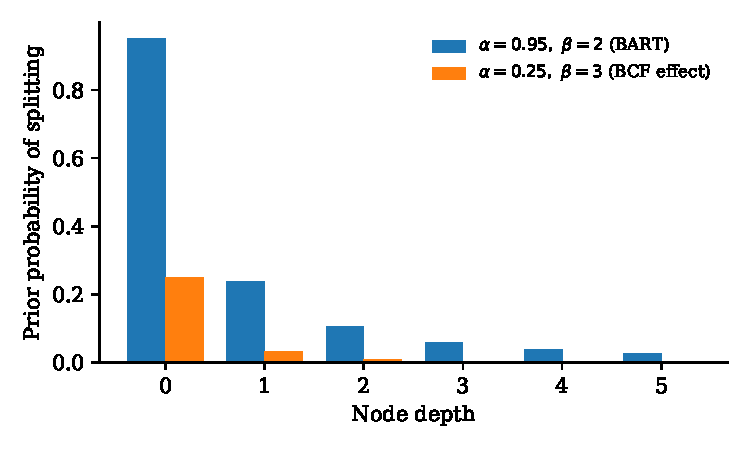
\includegraphics[width=0.85\linewidth]{bart_depth.pdf}
\caption{Prior probability that a node at each depth splits, for the BART default and for the more conservative effect forest of the Bayesian causal forest introduced below.}
\label{fig:bartdepth}
\end{figure}

\paragraph{Leaf values.} With the outcome rescaled to $[-0.5, 0.5]$, each leaf value has the prior
\[
\mu \sim N(0, \sigma_\mu^2), \qquad \sigma_\mu = \frac{0.5}{k\sqrt{m}},
\]
with default $k = 2$. The sum of $m$ independent leaf values then has prior standard deviation $0.5/k$, putting about 95\% of the prior mass for the regression function inside the observed range of the outcome.

\paragraph{Error variance.} A scaled inverse chi squared prior on $\sigma^2$, with $\nu = 3$ degrees of freedom, puts the least squares residual standard deviation at the 90th prior percentile for $\sigma$, favouring smaller error variance since BART is expected to fit better.

The default is $m = 200$ trees. Predictive performance usually levels off as $m$ grows and the leaf prior shrinks each tree more (Chipman, George and McCulloch 2010).

\subsection{Backfitting MCMC}

The posterior is
\begin{multline*}
p\bigl(\{\mathcal{T}_j, M_j\}_{j=1}^m, \sigma^2 \mid Y, X\bigr) \\
\propto \prod_{i=1}^n N\Bigl(y_i; \sum_{j=1}^m g(x_i; \mathcal{T}_j, M_j), \sigma^2\Bigr) \prod_{j=1}^m p(\mathcal{T}_j)\,p(M_j \mid \mathcal{T}_j)\; p(\sigma^2),
\end{multline*}
explored by Bayesian backfitting\index{Bayesian additive regression trees!backfitting MCMC|textbf}. Cycling over trees, each is updated given the others by forming the partial residual
\[
R_j = Y - \sum_{l \neq j} g(x; \mathcal{T}_l, M_l)
\]
and treating it as data for a single tree model. A Metropolis Hastings step\index{Markov chain Monte Carlo} updates the structure, proposing to grow a terminal node, prune two terminal children, change a splitting rule, or swap a parent and child rule. Given the structure, the leaf values have conjugate normal full conditionals and are integrated out analytically in the structure proposal. Finally $\sigma^2$ is drawn from its inverse gamma full conditional.



A known weakness is slow mixing: early trees can lock in splits that are hard to undo. The accelerated BART (XBART)\index{XBART|textbf} of He, Yalov and Hahn (2019) and He and Hahn (2023), the grow from root algorithm, rebuilds each tree by a stochastic search at each sweep and initializes the Markov chain. The \texttt{stochtree} software we use runs 20 such sweeps before the standard sampler in the applications (Chapter~\ref{ch:k401} and Section~\ref{sec:lalonde}) and 10 in the simulation below, substantially shortening burn in.

\section{Hill's causal BART}

Under ignorability, Hill's\index{Hill, Jennifer L.|textbf} (2011) causal BART\index{causal BART|textbf} fits the response surface $f(x, t) = \E(Y \mid X = x, T = t)$ with treatment as another covariate:
\begin{equation}
\E(Y \mid X = x, T = t) = \sum_{j=1}^m g(x, t; \mathcal{T}_j, M_j).
\label{eq:bart:hill}
\end{equation}
For each posterior draw $f^{(s)}$, the unit level contrast is $\tau^{(s)}(x_i) = f^{(s)}(x_i, 1) - f^{(s)}(x_i, 0)$, and the average effect is $n^{-1}\sum_i \tau^{(s)}(x_i)$. For the effect on the treated\index{effect on the treated} there are two accountings. Averaging the contrast over the $n_1$ treated units gives $n_1^{-1}\sum_{i: T_i = 1}\tau^{(s)}(x_i)$, the sample version of $\E\{\tau(X) \mid T = 1\}$. The applications in this book instead keep the observed outcome of each treated unit and impute only its missing control mean:
\[
\tau_{\mathrm{ATT}}^{(s)} = \frac{1}{n_1}\sum_{i: T_i = 1}\bigl\{Y_i - f^{(s)}(x_i, 0)\bigr\}.
\]
This holds the treated outcomes fixed and carries only the uncertainty about the control surface. A posterior for the realized effect $n_1^{-1}\sum_{i: T_i = 1}\{Y_i(1) - Y_i(0)\}$ would also draw each missing $Y_i(0)$ from the predictive distribution, adding the residual variance. The three can have similar centres and different widths, and Section~\ref{sec:lalonde} returns to the difference. This is the accounting identity\index{accounting identity} exactly: one fitted surface, every causal estimand an average over a chosen set of units, and posterior uncertainty about $f$ passed to each through the draws.

Hill's argument for modelling only the response surface, not the assignment, was practical: a flexible response model makes the propensity score\index{propensity score} unnecessary for bias removal, avoids the instability of weights, and gives coherent uncertainty for every target.

\paragraph{Binary outcomes.} For a binary outcome Chipman, George and McCulloch (2010) use probit BART, $\Prob(Y = 1 \mid x, t) = \Phi\{h(x, t)\}$ with a sum of trees prior on $h$ and $\Phi$ the standard normal distribution function, fitted by drawing a truncated normal latent variable for each unit and then updating the trees as above. The effects are differences of probabilities: each draw gives $\tau^{(s)}(x) = \Phi\{h^{(s)}(x, 1)\} - \Phi\{h^{(s)}(x, 0)\}$, averaged over the chosen units as before. The contrast $h(x, 1) - h(x, 0)$ lives on the latent scale and is not a risk difference, and in a Bayesian causal forest with a probit link the effect forest acts on that latent scale.

\begin{example}[The IHDP benchmark]
Hill built her simulation on the Infant Health and Development Program\index{Infant Health and Development Program|textbf}\index{IHDP|see{Infant Health and Development Program}}, a randomized trial of intensive home visits and child care for low birth weight, premature infants. She removed a nonrandom subset of the treated children, those with nonwhite mothers, so that the remaining treated and control groups differed systematically and overlap was imperfect, then simulated outcomes from known linear and nonlinear response surfaces so that the true effect was known. Under the nonlinear surface, BART had lower root mean squared error and better interval coverage than propensity score matching, inverse probability weighting and linear regression adjustment. The design has become a standard benchmark for heterogeneous effect methods.
\end{example}



\section{The overlap problem}

Weighting methods divide by the probability of the treatment received, so when the propensity is near zero or one the weights explode and a few observations dominate (Chapter~\ref{ch:ipw}).

\begin{definition}[Overlap]
Overlap, or positivity\index{overlap!positivity condition|textbf}, requires $0 < e(x) < 1$ for all $x$ in the support of the covariates, where $e(x) = \Prob(T = 1 \mid X = x)$.
\end{definition}

Overlap is an identification condition: without it the population average effect is not identified. But identification is a yes or no verdict, and overlap can be barely satisfied in some regions. Weighting puts the most weight exactly where the data are least informative.

A response surface model treats poor overlap\index{overlap!and extrapolation|textbf} as extrapolation\index{extrapolation|textbf}. Where only treated units are observed, $\mu_0(x)$ is extrapolated under the prior, and a model whose posterior widens there reports the uncertainty instead of hiding it in a weight. A Gaussian process does (Figure~\ref{fig:gpcausal}, right). A tree ensemble gives no such guarantee: past its last split a tree predicts with its edge leaf however far away the point lies, so the width of a BART interval need not grow with distance from the data. Its counterfactual uncertainty is still a useful diagnostic, but the widening is a property of the fitted model, not an automatic consequence of poor overlap.

\paragraph{Assessing common support.} Write $s_i^t$ for the posterior standard deviation of $f(x_i, t)$. A treated unit far from any control unit has a control outcome that BART must extrapolate, usually with a large $s_i^0$. Hill and Su (2013) turned this into a rule for discarding units that lack common support\index{overlap}. For the effect on the treated, their one standard deviation rule discards treated unit $i$ when
\[
s_i^0 > \max_{j: T_j = 1} s_j^1 + \operatorname{sd}_{j: T_j = 1}(s_j^1),
\]
so the uncertainty of each unit's counterfactual prediction\index{counterfactual!prediction|textbf} is compared with the uncertainty of the factual predictions in the same, treated, group. The LaLonde analysis of Section~\ref{sec:lalonde} uses a simpler variant, which compares each treated unit's $s_i^0$ with the 99th percentile of $s_j^0$ among the controls, whose outcomes are observed.

This alternative to propensity trimming\index{trimming} discards units because the outcome model cannot predict their counterfactuals, not because a separate model says they were unlikely to be treated. The criteria can disagree: a unit with an extreme propensity may have a well predicted counterfactual on a flat surface, though without nearby controls the model cannot see that flatness and may keep a unit whose counterfactual is wrong (Exercise~\ref{ex:chbart:6}). Conversely, a unit with a moderate propensity can have a poorly predicted counterfactual where the surface is steep and the other arm sparse. Report the effect on supported units, the fraction they represent, how many units were discarded and how the effect on the treated moved. A large move signals reliance on extrapolation.

\section{Bayesian causal forests}

Hahn, Murray and Carvalho (2020) identified and fixed two weaknesses of Hill's approach. Treating $T$ as an ordinary covariate lets BART shrink the treatment effect like every other split, which can produce regularization induced confounding\index{regularization induced confounding}\index{regularization induced confounding!in the BART setting|textbf} (Chapter~\ref{ch:horseshoe}). Under strong targeted selection\index{targeted selection|textbf}, units with the largest prognostic scores are most likely to be treated, and BART can misattribute effect to prognosis or the reverse and undercover badly. Its heterogeneity prior is also implicit: whatever the trees' splits on $T$ imply.

Their Bayesian causal forest (BCF)\index{Bayesian causal forest|textbf}\index{BCF|see{Bayesian causal forest}} separates the surface into a prognostic function\index{Bayesian causal forest!prognostic function|textbf} and an effect function\index{Bayesian causal forest!effect function|textbf},
\begin{equation}
Y_i = \mu\bigl(x_i, \hat e(x_i)\bigr) + \tau(x_i)\,T_i + \varepsilon_i,
\label{eq:bcf}
\end{equation}
with separate BART priors on $\mu$ and $\tau$. Two design choices matter.

\paragraph{The propensity as a covariate.} The estimated propensity $\hat e(x)$ enters the prognostic forest as an extra covariate\index{propensity score!as a covariate|textbf}, which the authors call targeted selection adjustment. A single split on $\hat e$ can then capture the confounding direction, protecting the effect estimate from regularization induced confounding. The coupled horseshoe of Chapter~\ref{ch:horseshoe} transplants this device from trees to sparse linear models.

\paragraph{A stronger prior on heterogeneity.} The effect forest uses 50 trees rather than 200, with $\alpha = 0.25$ and $\beta = 3$ discouraging splits. Effects are expected to vary less and more simply than outcomes. The prior keeps prognostic variation out of the effect forest, which stays near a constant unless the data support heterogeneity.

Tree depth sets how the effect varies; the leaf scale sets how much. Because leaf standard deviations scale as $m^{-1/2}$ (Exercise~\ref{ex:chbart:2}), fewer trees do not by themselves shrink the size of the effects, so Hahn, Murray and Carvalho (2020) also give each forest its own scale prior, half Cauchy for prognosis and half normal for the effect, the second pulling effects toward homogeneity. They also make the coding of the treatment part of the model, writing the effect term as $b_{T_i}\widetilde\tau(x_i)$ with $b_0$ and $b_1$ independent $N(0, 1/2)$ and $\tau(x) = (b_1 - b_0)\widetilde\tau(x)$, so that the prior does not depend on which arm is coded as zero.

The propensity covariate plays for a response surface a role like that of the orthogonal score in DML. In the linear version of Appendix~\ref{app:theory}, with the propensity direction known and its coefficient left unshrunk, it removes the first order sensitivity of the effect to shrinkage in the confounding direction. A forest shrinks splits on $\hat e$ like any other split, so for the Bayesian causal forest this remains a heuristic, supported by the simulations of Hahn, Murray and Carvalho (2020) rather than by a theorem.

\paragraph{Evidence from a competition.} The 2016 Atlantic Causal Inference Conference data analysis competition\index{Atlantic Causal Inference Conference competition|textbf}\index{ACIC|see{Atlantic Causal Inference Conference competition}}, analysed by Dorie, Hill, Shalit, Scott and Cervone in \emph{Statistical Science} in 2019, compared some thirty methods on many simulated data sets built from real covariates, with response surfaces and assignment mechanisms varied systematically. BART based methods were among the best for the average effect, and combinations of a flexible outcome model with some use of the propensity score did especially well.



\section{Theory}

BART long had excellent practice and thin theory\index{Bayesian additive regression trees!theory|textbf}; that has changed. Write $f_0$ for the true regression function, assumed $\zeta$ H\"older smooth on $[0,1]^p$ and depending on only $q \leq p$ coordinates.

\begin{theorem}[Posterior contraction for Bayesian forests, informal]\label{thm:bart}
Suppose $0 < \zeta \leq 1$ and that $\log p$ grows no faster than $n^{q/(2\zeta + q)}$. Under a modified BART prior\index{posterior contraction!for BART|textbf}, with a diffuse prior on the number of trees, a prior on the number of leaves that decays quickly enough and a sparsity inducing prior on the splitting variables, and under regularity conditions on $f_0$ and on the design, for every sequence $M_n \to \infty$
\[
\Pi\bigl(f : \|f - f_0\|_n > M_n\varepsilon_n \mid \mathcal{D}_n\bigr) \to 0 \quad \text{in } P_{f_0} \text{ probability},
\]
with $\varepsilon_n = n^{-\zeta/(2\zeta + q)}\log n$,
where $\Pi(\cdot \mid \mathcal{D}_n)$ is the posterior given the data $\mathcal{D}_n$ and $\|\cdot\|_n$ is the empirical $L_2$ norm at the design points.
\end{theorem}

The result is Theorem 5.1 of Ro\v{c}kov\'a and van der Pas (2020), which states the regularity conditions exactly; their Theorem 4.1 gives the rate with $\sqrt{\log n}$ for a single Bayesian tree, and their Theorem 6.1 the rate for sums of functions of different smoothness. Ro\v{c}kov\'a and Saha (2019) give a companion result for a slightly modified Chipman, George and McCulloch prior. This is the minimax rate for $q$ dimensional $\zeta$ smooth functions up to the logarithm, attained without knowing $\zeta$ or which $q$ covariates matter. The restriction $\zeta \leq 1$ is real, since step functions cannot exploit more smoothness, and it motivates soft trees\index{soft BART|textbf}. Linero and Yang (2018) showed that soft decision trees adapt to both smoothness and sparsity, and Linero's (2018) Dirichlet additive regression trees place a Dirichlet prior on the probabilities of splitting on each variable, so that irrelevant covariates are rarely used.

The theorem controls each arm only in its empirical design norm. To bound $\tau = \mu_1 - \mu_0$, the two arms need a common norm. If each contracts in $L_2(P_{X \mid T = t})$ and overlap is strict, $c \leq e(x) \leq 1 - c$ for some $c > 0$, then $\|h\|_{P_X} \leq \{\Prob(T = t)/c\}^{1/2}\|h\|_{P_{X \mid T = t}}$ transfers both rates to $L_2(P_X)$, and the triangle inequality gives $\tau$ the slower rate. The empirical to population step is not supplied by the theorem. Contraction alone also gives no Bernstein von Mises theorem for the average effect (Section~\ref{sec:crit:bayes} and Appendix~\ref{app:theory}).

The parallel with the horseshoe is close. A horseshoe lets a few large coefficients through and shrinks the rest; a Dirichlet sparse BART splits on a few variables and starves the rest. Both are global local priors in spirit.

\section{A simulation in the spirit of Hill}

To see how tree methods\index{Bayesian additive regression trees!simulation|textbf} behave with a nonlinear response surface and confounded assignment, we simulated 1,000 data sets\index{simulation study!BART in the spirit of Hill|textbf} for each of three assignment designs and two sample sizes, 500 and 2,000 units, with ten standard normal covariates. The prognostic surface was $\mu(x) = 2\sin(\pi x_1) + 1.5\,\mathbf{1}(x_2 > 0.5) + x_3^2$, the effect was $\tau(x) = 1 + 0.5x_4$, and the outcome was $Y = \mu(x) + \tau(x)T + \varepsilon$ with $\varepsilon \sim N(0, 1)$. Design A used propensity $\expit\{1.2x_1 + 0.8\,\mathbf{1}(x_2 > 0.5)\}$. The targeted designs used $0.01 + 0.98\,\expit[\gamma\{\mu(x) - \E\mu(X)\}/\mathrm{sd}\,\mu(X)]$, with $\gamma = 1$ for T1 and $\gamma = 3$ for T3: units with high prognostic scores were likely to be treated. The population mean and standard deviation of $\mu$ come from two million draws; the smallest and largest propensities in a data set average 0.17 and 0.98 under T1 and 0.02 and 0.99 under T3. The target was each data set's sample average of $\tau(x_i)$, not the population value 1; bias, root mean squared error and coverage are measured against it. We compared least squares with all covariates linear, Hill's BART, BART with the estimated propensity as an extra covariate (shown in the figure only), the Bayesian causal forest, and DML with the augmented score and random forest nuisances, all on the same data sets.

The tree methods ran on the \texttt{stochtree} 0.4.5 defaults, with 10 grow from root sweeps followed by four chains of 2,000 retained draws each, pooled, and not on the Chipman, George and McCulloch prior described above: the software standardizes the outcome, starts the leaf variance at about the variance of $y$ divided by $m$ and samples it, puts an inverse gamma prior with both parameters zero on $\sigma^2$, and gives the prognostic forest of the Bayesian causal forest 250 trees rather than 200. Tree intervals are the 2.5\% and 97.5\% posterior quantiles of the sample average effect. The forest took its propensity from a five fold cross validated logistic regression that is linear in $x$, and so misspecified, since the true propensity contains the indicator $\mathbf{1}(x_2 > 0.5)$ in design A and the whole prognostic surface in the targeted designs. DML used five fold cross fitting, random forests with 200 trees and minimum leaf size 5 for $\mu_0$, $\mu_1$ and $e$, propensities clipped to $[0.01, 0.99]$, and a Wald interval. Least squares reports a heteroskedasticity robust (HC3) interval.

\begin{figure}[ht]
\centering
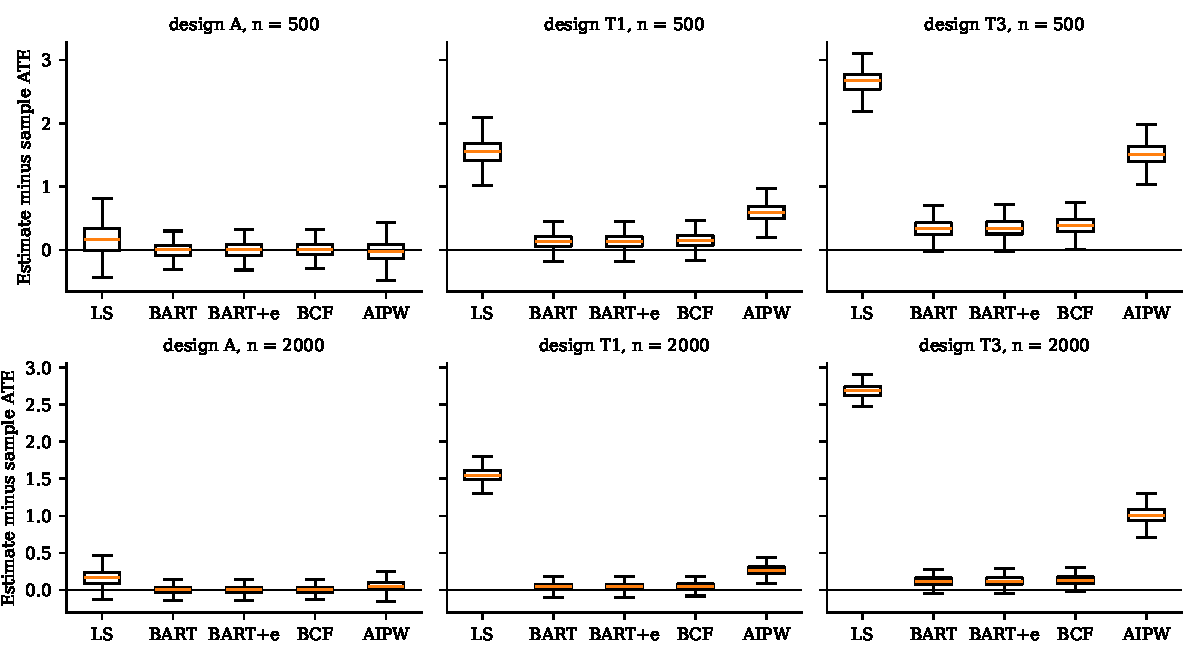
\includegraphics[width=\linewidth]{simbart.pdf}
\caption{Error of five estimators of the sample average effect, estimate minus truth, over 1,000 simulated data sets per panel, by assignment design (A, and targeted selection T1 and T3) and sample size. LS is least squares, BART+e is BART with the estimated propensity as a covariate, BCF the Bayesian causal forest and AIPW is DML with the augmented score; boxes show the quartiles.}
\label{fig:simbart}
\end{figure}

\begin{table}[ht]
\centering
\caption{Simulation results, 1,000 data sets per design and sample size. Design A is the confounded design of the text; T1 and T3 select on the prognostic surface with $\gamma = 1$ and 3. Coverage and width refer to 95\% intervals (HC3 for least squares), and the target is the sample average effect of each data set. The Monte Carlo standard error of a coverage near 0.9 is 0.01.}
\label{tab:simbart}
\small
\begin{tabular}{llcccc}
\toprule
Design, $n$ & Method & Bias & RMSE & Coverage & Width \\
\midrule
A, 500 & Least squares (HC3) & 0.17 & 0.29 & 0.880 & 0.93 \\
A, 500 & BART, Hill & 0.00 & 0.12 & 0.949 & 0.47 \\
A, 500 & Bayesian causal forest & 0.01 & 0.12 & 0.946 & 0.47 \\
A, 500 & DML, augmented score & $-0.03$ & 0.17 & 0.942 & 0.65 \\
\midrule
A, 2{,}000 & Least squares (HC3) & 0.17 & 0.21 & 0.705 & 0.46 \\
A, 2{,}000 & BART, Hill & 0.00 & 0.06 & 0.945 & 0.22 \\
A, 2{,}000 & Bayesian causal forest & 0.01 & 0.06 & 0.944 & 0.22 \\
A, 2{,}000 & DML, augmented score & 0.05 & 0.09 & 0.869 & 0.28 \\
\midrule
T1, 500 & Least squares (HC3) & 1.55 & 1.56 & 0.000 & 0.78 \\
T1, 500 & BART, Hill & 0.13 & 0.18 & 0.769 & 0.44 \\
T1, 500 & Bayesian causal forest & 0.15 & 0.19 & 0.720 & 0.44 \\
T1, 500 & DML, augmented score & 0.59 & 0.61 & 0.033 & 0.60 \\
\midrule
T1, 2{,}000 & Least squares (HC3) & 1.55 & 1.55 & 0.000 & 0.38 \\
T1, 2{,}000 & BART, Hill & 0.04 & 0.07 & 0.873 & 0.20 \\
T1, 2{,}000 & Bayesian causal forest & 0.05 & 0.07 & 0.826 & 0.20 \\
T1, 2{,}000 & DML, augmented score & 0.27 & 0.27 & 0.020 & 0.25 \\
\midrule
T3, 500 & Least squares (HC3) & 2.67 & 2.67 & 0.000 & 0.69 \\
T3, 500 & BART, Hill & 0.34 & 0.37 & 0.348 & 0.58 \\
T3, 500 & Bayesian causal forest & 0.39 & 0.42 & 0.239 & 0.58 \\
T3, 500 & DML, augmented score & 1.52 & 1.53 & 0.000 & 0.59 \\
\midrule
T3, 2{,}000 & Least squares (HC3) & 2.68 & 2.68 & 0.000 & 0.34 \\
T3, 2{,}000 & BART, Hill & 0.12 & 0.14 & 0.562 & 0.26 \\
T3, 2{,}000 & Bayesian causal forest & 0.13 & 0.15 & 0.483 & 0.26 \\
T3, 2{,}000 & DML, augmented score & 1.01 & 1.01 & 0.000 & 0.30 \\
\bottomrule
\end{tabular}
\end{table}

Figure~\ref{fig:simbart} and Table~\ref{tab:simbart} show why least squares fails: it cannot represent the sine and threshold terms that drive confounding. In design A the flexible methods remove most bias; the trees have the smallest error and intervals about three quarters as wide as DML's, with coverage close to 0.95. With 1,000 data sets, the Monte Carlo standard error of coverage near 0.95 is 0.007. DML's coverage falls from 0.942 at 500 units to 0.869 at 2,000, where its bias of 0.05 matters beside a shrinking interval. Targeted selection breaks every interval: the causal forest covers less than BART in every targeted cell, DML at most 0.033, and least squares never. More data shrink the trees' bias, from 0.34 to 0.12 at $\gamma = 3$, but also their intervals. The root mean squared error of $\tau(x_i)$ in design A at 500 units was 0.31 for each tree method; the DML estimator does not estimate these effects.

With 1,000 replications the tree posteriors cover close to the nominal level in the confounded design A and undercover badly under targeted selection\index{targeted selection}, which Hahn, Murray and Carvalho (2020) also found for BART. The Bayesian causal forest they proposed for that case did no better here, but its propensity came from a linear logistic fit that misses the shape of the true one, and we did not try a better estimate. The intervals pool four chains of 2,000 draws, and the standard deviation of an endpoint across chains, averaged over data sets, is 0.016 to 0.026 at 500 units and 0.007 to 0.011 at 2,000, small beside intervals 0.44 to 0.58 and 0.20 to 0.26 wide. The chains agree with one another, which does not prove they have converged, but the shortfall tracks the bias: at 500 units in design T3 the BART estimate is off by 0.34 on average with an interval 0.58 wide. Going to 2,000 units cuts the bias by more than the width (to 0.12 against 0.26 for BART), so coverage rises, yet it stays well below 0.95. That is a reason to check posterior calibration by simulation, with chains long enough, in any important application (Chapter~\ref{ch:computation}).

\section{Gaussian process causal inference}\label{sec:bart:gp}

Gaussian processes\index{Gaussian process|textbf} are a second nonparametric prior for a response surface. A Gaussian process $f \sim \mathrm{GP}(m, k)$ has a mean function $m(x)$ and a covariance kernel $k(x, x')$. With Gaussian errors and the kernel and noise parameters fixed, the posterior is again a Gaussian process, $f \mid \mathcal{D}_n \sim \mathrm{GP}(m_n, k_n)$, with $m_n$ and $k_n$ given by the usual conditioning formulas. For causal work\index{Gaussian process!causal inference|textbf} one places independent priors on $\mu_0$ and $\mu_1$, or separate priors on $\mu$ and $\tau$ as in \eqref{eq:bcf}, and reads off the posterior of $\tau(x) = \mu_1(x) - \mu_0(x)$, again a Gaussian process given those parameters; a prior on them makes it a mixture of Gaussian processes.

The kernel is the modelling decision. A squared exponential kernel\index{Gaussian process!squared exponential kernel|textbf} $k(x, x') = \exp\{-\|x - x'\|^2/(2\ell^2)\}$ makes the surface infinitely differentiable; a Mat\'ern kernel with parameter $\nu$ gives sample paths that are $\lceil\nu\rceil - 1$ times differentiable, which is often more realistic. Unlike a tree ensemble, a Gaussian process makes its uncertainty grow smoothly as $x$ moves away from the data, as one wants where overlap is poor. Ray and van der Vaart (2020) prove a semiparametric Bernstein von Mises theorem for the mean of a binary outcome in one treatment arm, using a Gaussian process prior and a Dirichlet process prior on the covariate distribution under smoothness conditions. Adding $\lambda/\hat e(x)$, with $\lambda$ a free coefficient, a relative of the Bayesian causal forest's device, weakens those conditions (Appendix~\ref{app:theory}). This inverse propensity direction is the mean's Riesz representer and the clever covariate of targeted learning: it lets the posterior move the regression and its mean without the prior's smoothing bias.

\begin{example}[Gaussian process regression discontinuity]
In a regression discontinuity design\index{regression discontinuity|textbf}, treatment is assigned when a running variable $R$ crosses a cutoff $c$, and the effect at the cutoff is the jump
\[
\tau(c) = \lim_{r \downarrow c}\E(Y \mid R = r) - \lim_{r \uparrow c}\E(Y \mid R = r).
\]
Branson, Rischard, Bornn and Miratrix (2019) give each side of the cutoff its own Gaussian process and take the difference of the two posteriors at $c$. The bandwidth of local polynomial methods is replaced by a kernel length scale that carries a prior and is integrated out; the posterior downweights observations far from the cutoff through the kernel, and the interval for the jump reflects the uncertainty about how far to look.
\end{example}

Figure~\ref{fig:gpcausal} shows both uses of a Gaussian process on simulated data, each panel a single data set. Every Gaussian process has a squared exponential kernel times a constant plus white noise, with all hyperparameters set by maximizing the marginal likelihood and then held fixed, so the posteriors condition on those values and do not integrate over the length scale as the method of Branson and coauthors does. In the left panel 300 units have a running variable $R$ uniform on $[-1, 1]$ and the outcome $Y = 0.8R + 0.6\sin(2R) + 0.5\,\mathbf{1}(R \geq 0) + \varepsilon$, a smooth nonlinear trend and a jump of 0.5 at zero, with noise standard deviation 0.3. Separate Gaussian processes give a posterior for the jump with mean 0.68 and standard deviation 0.09, so the truth sits just outside the 95\% interval: the posterior at a boundary rests on one side's data only, a known weakness of any smoother there and a reason Branson and coauthors attend carefully to the kernel. Here the true slope at the cutoff is 2.0, so near the boundary each side's posterior mean is pulled toward that side's own level, which tends to lower the left limit and raise the right limit; here the jump comes out too large. In the right panel, controls are observed only for $x < 0.4$ and treated units only for $x > -0.4$: 300 controls are uniform on $[-2, 0.4]$ with $\mu_0(x) = \sin(1.5x)$ and noise standard deviation 0.25, and only they enter the fit. The posterior for $\mu_0$ is tight where controls are observed, with standard deviation 0.02 at $x = -1$, and wide where only treated units are, 0.59 at $x = 1.5$. That widening is how a response surface model reports poor overlap.

\begin{figure}[ht]
\centering
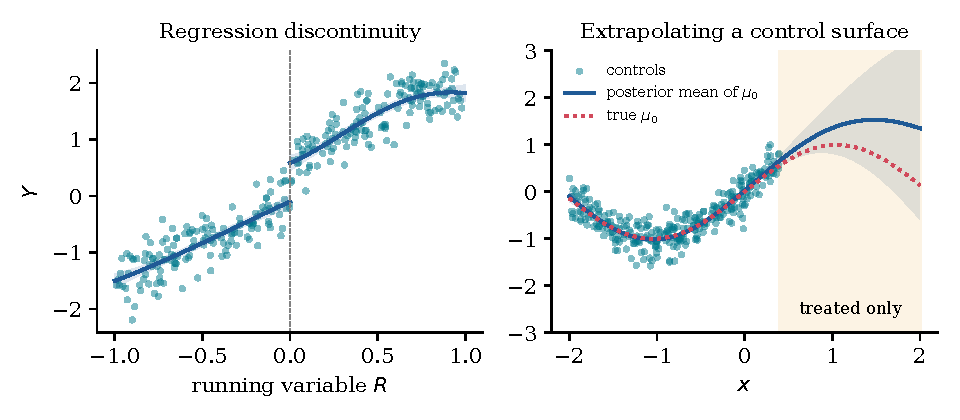
\includegraphics[width=\linewidth]{gp_causal.pdf}
\caption{Gaussian processes for causal inference. Left: a regression discontinuity, with separate posteriors on each side of the cutoff and bands of two posterior standard deviations. Right: the posterior for the control surface $\mu_0$ when controls are observed only to the left of the shaded region.}
\label{fig:gpcausal}
\end{figure}

The same logic serves panel and time series designs. Brodersen, Gallusser, Koehler, Remy and Scott (2015) fit a Bayesian structural time series before intervention, using untreated series as regressors under a spike and slab prior, and forecast the treated series' counterfactual path. The effect is the posterior predictive gap between the observed and forecast paths. This is a Bayesian relative of Abadie and Gardeazabal's (2003) synthetic control, replacing donor weights with a posterior over regression coefficients (Chapter~\ref{ch:did}). A Gaussian process can replace the state space model when a smooth function better describes the counterfactual path.

\section{Models and accounting, revisited}

Chapter~\ref{ch:mccullagh} argued that the average treatment effect is not a parameter of the data generating process but an accounting identity\index{accounting identity}\index{accounting identity!and BART|textbf}: an average of fitted contrasts over a chosen population. BART and Gaussian processes make this concrete: each effect is a prediction under the counterfactual assignment, averaged over the units of interest.

Ignorability concerns how the data arose, not the statistical model. It licenses the causal reading but does not select a method. Once it is accepted, the response surface approach says: build the best outcome model you can and read off the effects.

\begin{remark}[Causal and predictive models]
A model can predict observed outcomes well and still extrapolate badly to the counterfactual regime. Under targeted selection, plain BART can confound prognosis and effect despite an excellent fit. Under ignorability, good estimates of $\mu_0$ and $\mu_1$ across the whole covariate support give good effect estimates. This motivates the Bayesian causal forest's separation and propensity covariate.
\end{remark}

\section{Heterogeneous treatment effects}

BART estimates heterogeneous effects\index{heterogeneous treatment effects|textbf} $\tau(x)$\index{conditional average treatment effect} in \eqref{eq:bart:cate} without prespecified subgroups: trees splitting on both $x$ and $t$ capture effect modification\index{effect modification|see{heterogeneous treatment effects}}, those splitting mainly on $x$ capture prognosis. BCF's explicit separation \eqref{eq:bcf} improved calibration for $\tau(x)$ in Hahn, Murray and Carvalho (2020). Partially linear DML estimates a single weighted average (Chapter~\ref{ch:dml}); conditional effects need a basis expansion, the R learner or a causal forest, each a new estimator.

A posterior for $\tau(\cdot)$ gives one for any functional of it. The effect on the treated is $\E\{\tau(X) \mid T = 1\}$. The share of covariate profiles with positive conditional effect is $\Prob\{\tau(X) > 0\}$. Quantile treatment effects at level $u$, $F_{Y(1)}^{-1}(u) - F_{Y(0)}^{-1}(u)$, need the marginal laws of the potential outcomes, which only a model for the outcome distribution, not just its mean, supplies. The share of individuals who benefit, $\Prob\{Y(1) > Y(0)\}$, is different: it depends on the joint law of the two potential outcomes, which the data never identify, and Chapter~\ref{ch:tianpearl} bounds it using the results of Tian and Pearl (2000).

\section{Instruments and sensitivity, briefly}

When treatment is endogenous, ignorability fails and the response surface approach is inconsistent however flexible the surface. A valid instrument restores identification of a narrower target (Section~\ref{iv:sec:late}). The nonparametric extension puts BART or Gaussian process priors on both the first stage $\E(T \mid Z, X)$ and the structural function, with correlated errors linking the two equations, so that first stage uncertainty propagates through the joint posterior (Chapter~\ref{ch:iv}). Ignorability itself is untestable from the observed data; Section~\ref{sec:sensitivity} and Chapter~\ref{ch:tianpearl} ask how far a conclusion moves if it fails.

\section{Regularization and the prior as a selector}

The prior is a regularizer\index{prior distribution!as a regularizer|textbf}: BART penalizes tree complexity, BCF separates prognosis from effect, and a Gaussian process encodes smoothness and lets uncertainty grow where data are sparse. A lasso selects one fit by cross validation, and a DML interval is then computed from the selected nuisance fits, with orthogonality making their first order error negligible. BART instead averages over tree structures, depths and leaf values, carrying model uncertainty into the interval for $\tau$. Gaussian processes also integrate over kernel parameters when those carry priors; Figure~\ref{fig:gpcausal} instead fixes them at marginal likelihood estimates. Averaging does not guarantee calibration: Hill (2011) and Hahn, Murray and Carvalho (2020) find often near nominal average effect coverage, but the latter also find severe undercoverage under strong targeted selection\index{targeted selection}.

\begin{remark}[BART, adapted and purpose built]
BART was designed for regression and classification; its causal use is an adaptation, conditioning on ignorability, no interference and overlap imposed from outside. BCF is purpose built, putting the separation of confounding and effect modification into the prior. Hahn, Murray and Carvalho (2020) found it usually better for heterogeneity; plain BART with $T$ as a covariate is simpler and competitive for the average effect when selection is not strongly targeted.
\end{remark}

\section{The propensity score in a Bayesian model}

Rosenbaum\index{Rosenbaum, Paul R.!propensity score|textbf} and Rubin\index{Rubin, Donald B.!propensity score|textbf} (1983) showed that ignorability given $X$ implies ignorability given the propensity score\index{propensity score!Rosenbaum and Rubin theorem|textbf} $e(X)$, motivating matching\index{matching}, stratification and weighting. A Bayesian model can put a prior on $e$ and propagate its uncertainty, or use an estimate as an outcome covariate\index{propensity score!in a Bayesian model|textbf}, as BCF does.

The first way, applied to a weighting estimator such as the H\'ajek\index{Hajek estimator@H\'ajek estimator} ratio
\[
\hat\tau_{\mathrm{H}} = \frac{\sum_i T_iY_i/\hat e(X_i)}{\sum_i T_i/\hat e(X_i)} - \frac{\sum_i (1 - T_i)Y_i/\{1 - \hat e(X_i)\}}{\sum_i (1 - T_i)/\{1 - \hat e(X_i)\}},
\]
replaces $\hat e$ with posterior draws of $e$ and averages. This propagates propensity uncertainty but does not by itself reduce variance from extreme weights. Reducing it requires borrowing across units, as in Li's (2010) hierarchical model, Ghosh's (2015) binning and Sims's (2012) sieve (Datta and Polson 2026; Section~\ref{sec:weak}). Response surfaces borrow through the outcome model; adding the propensity covariate retains the selection information required by the Robins, Ritov and Wasserman example (Section~\ref{sec:weak}).

\section{Trees and the horseshoe compared}

Trees\index{Bayesian additive regression trees!compared with the horseshoe|textbf} approximate smooth functions with many steps and are least efficient for a smooth low order polynomial, which a horseshoe on a polynomial or spline basis captures directly. Trees find interactions unprompted; a basis must include them, and their number grows quickly with dimension. Horseshoe coefficients are interpretable and their shrinkage factors diagnostic; tree ensembles are read through predictions.

 The simulation of Table~\ref{tab:simbart} is a case where trees are the right tool, since the sine and threshold terms in the prognostic surface are exactly what a linear basis misses and what the trees found; the coupled horseshoe simulation of Chapter~\ref{ch:horseshoe} is the opposite case, with many covariates, few of them relevant, and a sparse linear structure that a tree would approximate with many steps.

In Chapter~\ref{ch:k401} we report both. Agreement suggests the conclusion does not depend on functional form; disagreement is a finding. Fit the horseshoe first when a linear or additive baseline is plausible, trees first for hundreds or thousands of units with expected interactions or thresholds, and the other as a check whenever the answer matters. The book has no comparison of the two with $p$ near or above $n$, and the horseshoe results there are mixed: at $n = 200$, $p = 150$ or 300 with five strong confounders, DML was more accurate than every horseshoe posterior; with thirty weak confounders at $p = 150$, the coupled posterior was more accurate than DML (Section~\ref{sec:ricsim}).

\section{BART, DML and generative computation}

Table~\ref{tab:bart:compare} compares response surface models\index{Bayesian additive regression trees!compared with double machine learning|textbf}, DML (Chapters~\ref{ch:dml} and~\ref{ch:critique}) and generative Bayesian computation (GBC, Chapter~\ref{ch:computation}). All assume ignorability here. BART and DML differ in model and target; GBC changes computation, learning a quantile map for any model it is trained on, including a forest prior.

\begin{table}[ht]
\centering
\small
\caption{Three approaches to effects under ignorability.}
\label{tab:bart:compare}
\setlength{\tabcolsep}{3pt}
\begin{tabular}{@{}L{0.9in}L{1.1in}L{1.1in}L{1.1in}@{}}
\toprule
 & BART and BCF & DML & GBC \\
\midrule
Model & outcome surface & two nuisance regressions & any model it is trained on, as a quantile map \\
Main target & conditional effects & one scalar per score & any functional, including quantiles \\
Uncertainty & posterior & asymptotic interval & posterior of that model, approximated \\
Poor overlap & extrapolation under the prior; width model dependent & large score variance, or trimming that changes the target & inherited from the model \\
Risk preferences & by postprocessing draws & not directly & distortions applied to learned quantiles \\
Dynamic treatments & limited & limited & sequential decisions \\
Propensity & optional covariate & required & optional \\
Software & mature & mature & developing \\
\bottomrule
\end{tabular}
\end{table}

BART and BCF suit unknown effect heterogeneity and moderate samples, from a few hundred to a few thousand units, when a posterior for every effect and mature software matter. DML suits a single scalar, a large sample, an acceptable partially linear or interactive model, and cheap computation. GBC suits decisions requiring the whole distribution of utility under each action, risk preferences beyond expected value, or sequential actions. No method dominates. GBC changes computation while aiming at the same posterior, and pays when one trained network serves many data sets from the same model.

\section{Software and computation}

BART software\index{Bayesian additive regression trees!software|textbf} includes Chipman, George and McCulloch's \texttt{BayesTree}\index{BayesTree|textbf}; Sparapani, Spanbauer and McCulloch's (2021) \texttt{BART}\index{software!BART packages|textbf}, which adds survival outcomes; Hahn, Murray and Carvalho's \texttt{bcf} for BCF; \texttt{bartCause} for Hill's method; and \texttt{stochtree}\index{stochtree|textbf}, used for this book's tree fits (Appendix~\ref{app:code}).

Several variants matter for causal work. Soft BART\index{soft BART}, due to Linero and Yang (2018) and discussed above, replaces hard splits with smooth gates and adds a sparsity prior on the splitting variables. XBART\index{XBART}, the grow from root algorithm described earlier, scales to much larger samples than the original local moves. Particle Gibbs, as developed by Lakshminarayanan, Roy and Teh (2015), improves mixing by replacing local birth and death moves with a sequential Monte Carlo update of whole trees.

Gaussian process models can be fitted with Stan or Python libraries for moderate $n$, and the inducing point approximations of Titsias (2009) extend them to tens of thousands of observations.



\section{In practice}

\paragraph{The target.} The targets are the average effect, the effect on the treated and the conditional effect $\tau(x)$. Each posterior draw of the BART surface, or of the Bayesian causal forest pair $(\mu, \tau)$ in \eqref{eq:bcf}, gives the fitted contrast at every unit; averaging over all units, treated units or any subgroup gives each target, and Hill's common support rule uses the same draws to choose which units.

\paragraph{What the analyst does differently.} An analyst who fits a response surface states ignorability and overlap at the outset and then treats the rest as regression. When selection may be targeted she fits the Bayesian causal forest as well as plain BART, and she takes care over its propensity, since with a misspecified one the forest did no better than BART in Table~\ref{tab:simbart}. She applies Hill and Su's rule and reports how many units it discards and how the effect on the treated moves. She checks calibration on simulated data of the same design before reporting an interval, because a posterior is not automatically calibrated: in Table~\ref{tab:simbart} the tree intervals cover close to the nominal 0.95 in design A and fall well below it under targeted selection. And she reports $\tau(x)$ and its functionals from the same draws as the average.

\paragraph{Against DML.} For the average effect alone design A at 500 units was close: root mean squared error 0.12 for both tree methods against 0.17 for DML, and DML's wider interval covered 0.942 of the data sets where the trees covered 0.949 and 0.946. At 2,000 units DML's coverage fell to 0.869, and under targeted selection every method undercovers and DML is the worst of the three flexible ones. DML is cheaper, but in this simulation it was not the safer choice even for the scalar: the trees had smaller root mean squared error in every cell. DML as run in Table~\ref{tab:simbart} also does not estimate $\tau(x_i)$, which the trees recovered with root mean squared error 0.31 in design A at 500 units; where overlap fails its interval widens through the inverse propensities in its score, or its target changes when it trims; and its support diagnostics come from the propensity model, not from the uncertainty of the counterfactual predictions. The limits are the ones the chapter has stated: the posterior is not automatically calibrated, contraction for the function is not by itself a Bernstein von Mises theorem for the average, and sampling trees costs more than a cross fitted regression.

\section*{Notes}

Rubin (1978) gives the Bayesian response surface formulation, predicting missing potential outcomes from a model. Hahn, Carvalho, Puelz and He (2018) study regularization induced confounding. For general posterior contraction theory see Ghosal and van der Vaart (2017), and for a BART review Hill, Linero and Murray (2020). Frequentist tools for conditional effects include the causal forest of Wager and Athey (2018) and the R learner of Nie and Wager (2021).

\begin{exercises}
\item\label{ex:chbart:1} Compute the prior probability that a BART tree has exactly one, two and three terminal nodes under $\alpha = 0.95$ and $\beta = 2$.
\item\label{ex:chbart:2} Show that with $m$ trees and leaf prior standard deviation $0.5/(k\sqrt{m})$, the prior standard deviation of the regression function at any $x$ is $0.5/k$, independent of $m$.
\item\label{ex:chbart:3} Derive the conjugate full conditional of the leaf values of one tree given its structure and the partial residuals.
\item\label{ex:chbart:4} Explain why treating $T$ as an ordinary covariate in BART can produce regularization induced confounding, using the argument of Chapter~\ref{ch:horseshoe}.
\item\label{ex:chbart:5} Show that the BCF prior with a constant effect forest reduces to a partially linear model with a BART prognostic function.
\item\label{ex:chbart:6} Design a simulation in which Hill's common support rule and propensity trimming discard different units, and compare the resulting estimates of the effect on the treated.
\item\label{ex:chbart:7} For a Gaussian process regression discontinuity with squared exponential kernels on each side of the cutoff, write the posterior mean and variance of the jump $\tau(c)$ in closed form given the length scales, signal variance and noise variance, and explain how a prior on the length scales replaces bandwidth selection.
\end{exercises}

\part{Identification beyond Ignorability}
\chapter{Instruments}\label{ch:iv}
\newcommand{\ivwrightols}{$-$0.50}
\newcommand{\ivwrightiv}{$-$1.01}
\newcommand{\ivcardn}{3{,}010}
\newcommand{\ivcardols}{0.075}
\newcommand{\ivcardolsse}{0.003}
\newcommand{\ivcardfs}{0.32}
\newcommand{\ivcardfsse}{0.09}
\newcommand{\ivcardF}{13.3}
\newcommand{\ivcardtsls}{0.132}
\newcommand{\ivcardtslsse}{0.055}
\newcommand{\ivcardrfmed}{0.131}
\newcommand{\ivcardrflo}{0.043}
\newcommand{\ivcardrfhi}{0.249}
\newcommand{\ivcardrfpgt}{0.86}
\newcommand{\ivcardsmed}{0.135}
\newcommand{\ivcardslo}{0.039}
\newcommand{\ivcardshi}{0.270}
\newcommand{\ivcardspgt}{0.86}
\newcommand{\ivcardrho}{$-$0.29}
\newcommand{\ivcardrholo}{$-$0.71}
\newcommand{\ivcardrhohi}{0.17}
\newcommand{\ivweakF}{1.7}
\newcommand{\ivmanyF}{1.0}
\newcommand{\ivweakols}{0.70}
\newcommand{\ivweakiqrlo}{$-$0.43}
\newcommand{\ivweakiqrhi}{0.59}
\newcommand{\ivmanytsls}{0.66}
\newcommand{\ivweakbmed}{0.34}
\newcommand{\ivweakbcov}{98\%}
\newcommand{\ivmanybcov}{11\%}
\newcommand{\ivhiercov}{98\%}
\newcommand{\ivrflen}{7.3}
\newcommand{\ivrfcov}{98\%}
\newcommand{\ivrfmed}{0.29}
\newcommand{\ivweakblen}{5.2}
\newcommand{\ivmanybmed}{0.66}
\newcommand{\ivmanyblen}{0.60}
\newcommand{\ivhiermed}{0.58}
\newcommand{\ivhierlen}{3.1}
\newcommand{\ivhierrhat}{1.03}
\newcommand{\ivscalesmall}{14}
\newcommand{\ivscaleten}{1.9}
\newcommand{\ivscalehund}{0.77}
\newcommand{\ivscalehundcov}{4\%}
\newcommand{\ivcardrhopneg}{0.86}
\newcommand{\ivcardrhat}{1.000}
\newcommand{\ivcardess}{29{,}282}
\newcommand{\ivchexactmed}{0.12}
\newcommand{\ivchexactlen}{4.8}
\newcommand{\ivchexactcov}{100\%}
\newcommand{\ivchblockdiff}{0.01}
\newcommand{\ivcholdmed}{0.28}
\newcommand{\ivcholdlen}{0.78}
\newcommand{\ivcholdcov}{45\%}
\newcommand{\ivcholddiff}{0.22}
\newcommand{\ivcholdlonglen}{2.6}
\newcommand{\ivcholdlongcov}{80\%}
\newcommand{\ivchcardsd}{0.078}
\newcommand{\ivchcardoldrhat}{1.21}
\newcommand{\ivchcardoldess}{13}
\newcommand{\ivchcardoldlag}{0.995}
\newcommand{\ivchcardoldstep}{0.005}
\newcommand{\ivscaledeflen}{5.2}
\newcommand{\ivscaledefcov}{97\%}
\newcommand{\ivscalecovsmall}{97\%}
\newcommand{\ivscalecovone}{96\%}
\newcommand{\ivscalemedsmall}{0.20}
\newcommand{\ivscalemedhund}{0.64}
\newcommand{\ivhwtsls}{0.64}
\newcommand{\ivhwflatcov}{9\%}
\newcommand{\ivhwflatlen}{0.59}
\newcommand{\ivhwhiermed}{0.56}
\newcommand{\ivhwhiercov}{98\%}
\newcommand{\ivhwhierlen}{3.1}
\newcommand{\ivhwhierrhat}{1.03}
\newcommand{\ivhwhiersh}{99.7\%}
\newcommand{\ivhwhsmed}{0.59}
\newcommand{\ivhwhscov}{99\%}
\newcommand{\ivhwhslen}{5.5}
\newcommand{\ivhwhsrhat}{1.02}
\newcommand{\ivhwhssh}{99.8\%}
\newcommand{\ivhstsls}{0.17}
\newcommand{\ivhsflatmed}{0.17}
\newcommand{\ivhsflatcov}{77\%}
\newcommand{\ivhsflatlen}{0.25}
\newcommand{\ivhshiermed}{0.08}
\newcommand{\ivhshiercov}{88\%}
\newcommand{\ivhshierlen}{0.32}
\newcommand{\ivhshierrhat}{1.00}
\newcommand{\ivhshsmed}{0.10}
\newcommand{\ivhshscov}{89\%}
\newcommand{\ivhshslen}{0.30}
\newcommand{\ivhsrhat}{1.00}


\begin{tcolorbox}[colback=gray!6,colframe=gray!50,title=In brief,fonttitle=\normalfont\itshape,coltitle=black,colbacktitle=gray!15,boxrule=0.4pt,arc=1pt]
Instruments identify effects under unmeasured confounding at the price of an exclusion restriction. The local average effect is an accounting over compliers. With one weak instrument a posterior reports the weakness as a wide interval, whether the prior is on the reduced form or on the structural model, though the structural width is set by the prior on the error covariance. With twenty weak instruments a diffuse structural prior is confident and wrong, and a shrunk first stage gives intervals that cover the truth by being wide. Kernel methods are used for nonlinear structural functions, a global local prior is proposed for them, and Mendelian randomization turns Fisher's genetic confounder into an instrument.
\end{tcolorbox}

When confounders are unmeasured, adjustment fails\index{ignorability!failure of|textbf}, but another source of variation may rescue the analysis. An instrument\index{instrument|see{instrumental variable}}\index{instrumental variable|textbf} moves treatment, has no direct effect on the outcome, and is itself unconfounded. The idea is a century old.

\section{A short history of the instrument}\label{iv:sec:history}

\paragraph{Wright, 1928.} The instrumental variable\index{instrumental variable!history of|textbf} was invented for a question about tariffs. Appendix B of Philip Wright\index{Wright, Philip G.|textbf}'s \emph{The Tariff on Animal and Vegetable Oils} (Wright 1928) asks how to estimate supply and demand elasticities when price and quantity are determined together, so the observed points are intersections of two shifting curves and a regression of quantity on price traces neither. Wright\index{Wright, Philip G.!instrumental variable|textbf}'s answer was a variable that shifts one curve and not the other. A factor that moves supply, such as weather or yield per acre, while leaving demand alone moves the equilibrium along the demand curve, and the ratio of its covariances with quantity and with price recovers the demand slope. He applied the method to butter and flaxseed. Authorship has been debated, because Philip's son Sewall Wright\index{Wright, Sewall|textbf} had invented path analysis\index{path analysis} (Wright 1921, 1934); Stock and Trebbi (2003) attribute the appendix to Philip by stylometry, its path diagrams\index{Wright, Sewall!path diagrams|textbf} reflecting the collaboration of father and son.

Figure~\ref{fig:wright} reproduces Wright's problem. In 200 simulated markets demand is $q = 10 - p + u_d$ and supply is $q = 2 + 0.8p + 1.5w + u_s$, where the supply shifter $w$, call it weather, and the shocks $u_d$ and $u_s$ are independent standard normal. The cloud of equilibria slopes downward, but least squares gives \ivwrightols, a compromise between the two curves. The instrumental variable estimate, the covariance of weather with quantity divided by its covariance with price, is \ivwrightiv.

\begin{figure}[htbp]
\centering
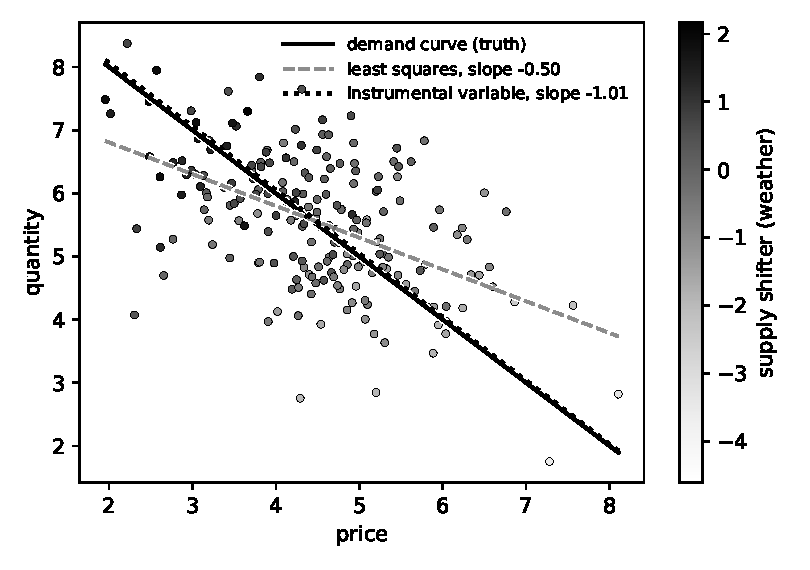
\includegraphics[width=0.85\linewidth]{fig_wright.pdf}
\caption{Wright's problem. Equilibrium prices and quantities in 200 simulated markets, shaded by the supply shifter, darker for larger values. Least squares fits a compromise between the supply and demand curves; the instrumental variable estimate recovers the demand slope of $-1$.}
\label{fig:wright}
\end{figure}

\paragraph{Haavelmo and the Cowles Commission, 1943 to 1950.} The appendix was largely ignored, and the idea returned through simultaneous equations\index{simultaneous equations}. Haavelmo\index{Haavelmo, Trygve} (1943) showed that least squares in a simultaneous system is biased because regressor and error are correlated. Haavelmo (1944) treated econometric models as probability models, with autonomous structural equations and the reduced form into which they solve. In this framework exogenous variables play the role of Wright's shifters: one excluded from an equation identifies that equation's coefficients. The Cowles Commission\index{Cowles Commission|textbf} turned this into the theory of identification, with the order and rank conditions for linear systems and full information maximum likelihood (Koopmans, Rubin and Leipnik 1950), and limited information maximum likelihood (Anderson and Rubin 1949), whose accompanying test for the structural coefficient is still the weak instrument robust test of choice.

\paragraph{Reiers\o l, Geary and the name.} Olav Reiers\o l\index{Reiersol, Olav@Reiers\o l, Olav!the name instrumental variables|textbf} introduced the method in 1941 and the name instrumental variables\index{instrumental variable} in 1945, extending Frisch's (1934) confluence analysis of linear relations among mismeasured variables. Geary (1949) developed it for errors in variables\index{errors in variables|see{measurement error}}. The instrument correlates with the true regressor but not its measurement error.

\paragraph{Madansky.} Albert Madansky\index{Madansky, Albert!instruments for errors in variables|textbf} reviewed instruments alongside other methods for fitting lines when both variables have measurement error (Madansky 1959), then carried them to factor analysis (Madansky 1964), where indicators of one factor instrument another. For Madansky an instrument was an assumption about the covariance structure of unobservables, and its credibility a question about the science.

\paragraph{Two stage least squares and beyond.} Theil (1953) and Basmann (1957) introduced two stage least squares\index{two stage least squares|textbf}, and Sargan (1958) gave the general theory of instrumental variable estimation, including the test of overidentifying restrictions.  Imbens and Angrist (1994) and Angrist, Imbens and Rubin\index{Rubin, Donald B.!local average treatment effect|textbf} (1996) showed that with heterogeneous effects the instrument identifies the effect among compliers (Section~\ref{iv:sec:late}), and Bound, Jaeger and Baker (1995) and Staiger and Stock (1997) showed how badly the classical estimators behave when the instrument is weak.

\section{The linear model}
\begin{figure}[ht]
\centering
\begin{tikzpicture}[node distance=16mm]
\node[v] (Z) {$Z$};
\node[v,right=of Z] (T) {$T$};
\node[v,right=of T] (Y) {$Y$};
\node[h,above=10mm of $(T)!0.5!(Y)$] (U) {$U$};
\draw[e] (Z) -- (T); \draw[e] (T) -- (Y); \draw[e] (U) -- (T); \draw[e] (U) -- (Y);
\end{tikzpicture}
\caption{An instrument $Z$ moves treatment $T$, has no direct path to $Y$, and is independent of the unmeasured confounder $U$, shown dashed.}
\label{fig:dagiv}
\end{figure}


Consider the model of Figure~\ref{fig:dagiv},
\begin{align*}
Y &= \tau T + \delta U + \varepsilon, \\
T &= \pi Z + \gamma U + \nu,
\end{align*}
where $U$ is an unmeasured confounder and $Z$, $U$, $\varepsilon$ and $\nu$ are independent. Least squares of $Y$ on $T$ is biased by $\delta\gamma\,\mathrm{Var}(U)/\mathrm{Var}(T)$. The instrumental variable estimator\index{instrumental variable!linear model|textbf}
\[
\hat\tau_{\mathrm{IV}} = \frac{\widehat{\mathrm{Cov}}(Z, Y)}{\widehat{\mathrm{Cov}}(Z, T)}
\]
is consistent when $\pi \neq 0$, since $\mathrm{Cov}(Z, Y) = \tau\,\mathrm{Cov}(Z, T)$.

Figure~\ref{fig:iv} uses 500 replications of size 500 with $\tau = 1$, independent standard normal $Z$, $U$, $\nu$ and $\varepsilon$, $T = 0.5Z + U + \nu$ and $Y = \tau T + 2U + \varepsilon$. Here $\pi = 0.5$, $\gamma = 1$, $\delta = 2$ and $\mathrm{Var}(T) = 2.25$, so least squares has bias $2/2.25 = 0.89$ and averages 1.89. The instrumental variable estimate has median 1.01 and about four times the spread of least squares. With a first stage $F$ of about 60 it is roughly normal; Section~\ref{iv:sec:weak} shows the heavy tails of weak instruments.

\begin{figure}[ht]
\centering
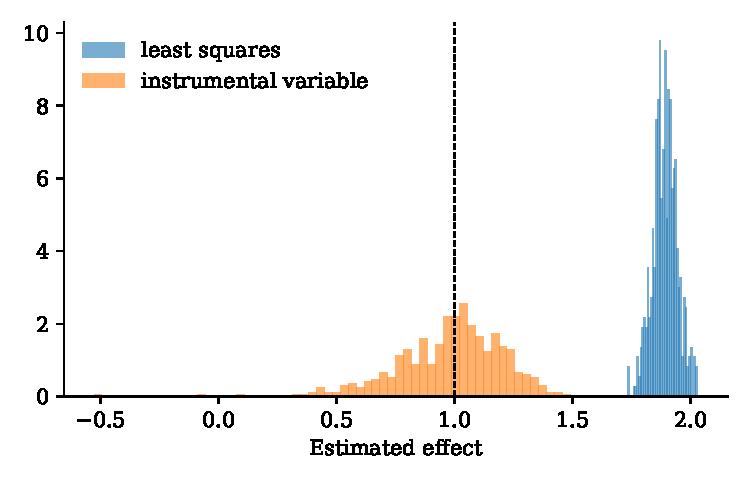
\includegraphics[width=\linewidth]{iv.pdf}
\caption{Sampling distributions of least squares and instrumental variable estimates of $\tau = 1$ with an unmeasured confounder, 500 replications of size 500.}
\label{fig:iv}
\end{figure}

The IV\index{IV|see{instrumental variable}} estimator is a ratio, unstable when the denominator is near zero, and with one instrument and normal errors its finite sample distribution has no mean. 

\section{The local average treatment effect}\label{iv:sec:late}

With heterogeneous effects and binary $Z$ and $T$, let $T(z)$ be the potential treatment under instrument value $z$. Units are compliers\index{complier|textbf} if $T(1) = 1$ and $T(0) = 0$, always takers\index{always taker|textbf} if $T(1) = T(0) = 1$, never takers\index{never taker|textbf} if $T(1) = T(0) = 0$, and defiers\index{defier|textbf} if $T(1) = 0$ and $T(0) = 1$.

\begin{theorem}[Imbens and Angrist; Angrist, Imbens and Rubin]
Under random assignment of $Z$, the exclusion restriction\index{exclusion restriction|textbf} that $Z$ affects $Y$ only through $T$, monotonicity\index{monotonicity|textbf} (no defiers), and a nonzero first stage,
\[
\frac{\E(Y \mid Z = 1) - \E(Y \mid Z = 0)}{\E(T \mid Z = 1) - \E(T \mid Z = 0)} = \E\{Y(1) - Y(0) \mid \text{complier}\}.
\]
\end{theorem}

The left side is the Wald ratio\index{Wald estimator|textbf}\index{Wald ratio|see{Wald estimator}}; the right is the local average treatment effect\index{local average treatment effect|textbf}\index{LATE|see{local average treatment effect}}, the effect among those whose treatment the instrument moves. The intuition is an accounting. Random assignment makes the two arms comparable, so the numerator, the effect of $Z$ on $Y$, is a sum over the four strata. Always takers and never takers receive the same treatment under either value of the instrument, so by exclusion they contribute nothing; monotonicity removes the defiers, whose contribution would enter with the opposite sign. What remains is the complier share times the complier effect. The denominator, nonzero by assumption, is the complier share, the fraction of units the instrument moves. Dividing one by the other leaves the complier effect.

The local effect is an accounting identity\index{accounting identity} with $Q$ the covariate law of compliers, chosen by the instrument rather than the analyst, provided that, given covariates, compliers have the same average effect as everyone else. Report the complier share, because a Wald ratio built on a small share is a statement about few people, and the heavy tails of Figure~\ref{fig:weakiv} are near. Describe the compliers: when the assumptions hold given covariates $X$, their covariate law is identified as $Q_c(dx) \propto \pi_c(x)\,P(dx)$, where $\pi_c(x) = \E(T \mid Z = 1, X = x) - \E(T \mid Z = 0, X = x)$ is the complier share at $x$. And do not present the number as the average effect in the population unless a model extends it there (Section~\ref{iv:sec:accounting}).

\section{Bayesian instrumental variables}

Imbens and Rubin\index{Rubin, Donald B.!Bayesian instrumental variables|textbf} (1997) gave a Bayesian analysis of the binary instrument model\index{instrumental variable!Bayesian|textbf}. The principal strata, compliers, always takers and never takers, are latent, but $(Z, T)$ partly reveals them: a unit with $Z = 1$ and $T = 0$ must be a never taker, while one with $Z = 1$ and $T = 1$ is a complier or an always taker. Data augmentation imputes the missing strata, and the outcome model in each stratum is fitted to the completed data.

The Bayesian analysis respects the model's constraints: stratum proportions are nonnegative and outcome distributions proper, whereas the moment calculation behind the Wald ratio, applied to outcome distributions rather than means, can give complier densities that are negative in finite samples. It also delivers effects for always takers and never takers under explicit priors, separating what is learned from data and what from assumption.

\paragraph{Other Bayesian approaches.} The structural tradition models treatment and outcome jointly with correlated errors, so the posterior of the structural coefficient propagates first stage uncertainty rather than plugging in a fit. Kleibergen and Zivot (2003) compared diffuse priors in the structural and reduced form parametrizations, a comparison taken up in Section~\ref{iv:sec:weak}. Chib and Hamilton (2002) gave semiparametric Bayesian treatment models with an error distribution not fixed in advance. Conley, Hansen, McCulloch and Rossi (2008) replaced bivariate normal errors with a Dirichlet process mixture, avoiding a parametric error model. Conley, Hansen and Rossi (2012) placed a prior on the instrument's direct effect on the outcome, so exclusion need hold only approximately, the plausibly exogenous instruments of their title. The natural nonparametric extension puts BART or Gaussian process priors on both the first stage and the structural function, the joint posterior carrying uncertainty from one to the other.

\paragraph{Selection models.} The bivariate normal selection model of Chapter~\ref{ch:frameworks} (equation~\eqref{ss:eq:mills}) is the same structural idea with a latent selection equation in place of a linear first stage. Given the latent propensity $T^\ast$, the selection error $V$ is known, and the outcome equation is a regression with the added term $\rho\sigma V$ and residual variance $\sigma^2(1-\rho^2)$. Given the parameters and the outcome, each $T^\ast_i$ is normal with variance $1-\rho^2$ and mean equal to the selection index plus $\rho/\sigma$ times the outcome residual $Y_i - X_i^\top\beta - \tau T_i$, truncated to be positive when $T_i = 1$ and negative otherwise, so a Gibbs sampler alternates between the two (Chib and Hamilton 2002). With a weak or absent instrument the data barely identify the correlation $\rho$. Setting $\rho = 0$ is ignorability. Without an excluded instrument, what the data say about $\rho$ comes from the normal tails, and a prior on $\rho$ leaves that restriction in place. A prior concentrated near zero but not at it usually widens the posterior of $\tau$ when the data say little about $\rho$, but nothing guarantees it. Read this way, $\rho$ is a sensitivity parameter and the prior on it is the sensitivity analysis of Section~\ref{sec:sensitivity}: report how that posterior moves as the prior spreads.

\section{Weak instruments, Bayesian style}\label{iv:sec:weak}

When the first stage\index{first stage|textbf} is weak\index{weak instrument|textbf}, the instrumental variable\index{instrumental variable} estimator is badly biased toward least squares when there are many instruments and erratic when there is one, and in both cases its confidence intervals undercover. The Anderson and Rubin\index{Anderson and Rubin test|textbf} (1949) test of $\tau = \tau_0$ asks whether the instrument has any effect on $Y - \tau_0 T$ once the controls are in the regression. Its 90\% confidence set collects the values $\tau_0$ not rejected and has the stated coverage whatever the strength of the first stage, exactly with normal homoskedastic errors and approximately in large samples otherwise. With one instrument it is unbounded when the first stage $F$ statistic falls below the test's critical value. The Bayesian response\index{weak instrument!Bayesian treatment|textbf} is simpler. Write the reduced form\index{reduced form|textbf} as
\[
Y = \pi_Y Z + u_Y, \qquad T = \pi_T Z + u_T,
\]
so that $\tau = \pi_Y/\pi_T$. In the notation of the linear model $\pi_T = \pi$, $\pi_Y = \tau\pi$, $u_T = \gamma U + \nu$ and $u_Y = \tau u_T + \delta U + \varepsilon$. The posterior for $(\pi_Y, \pi_T)$ is well behaved whatever their size. The posterior for $\tau$ is the law of their ratio, wide and heavy tailed when $\pi_T$ is near zero, because the data then say little about $\tau$.

Kleibergen and Zivot showed that with weak instruments the parametrization matters: priors flat in the structural form can be informative in the reduced form, and the reverse. The reduced form is the natural place to start. Because $\pi_Y = \tau\pi_T$, a prior flat in $(\pi_Y, \pi_T)$ is proportional to $|\pi_T|$ in the coordinates $(\tau, \pi_T)$, so it puts little weight on a small first stage, whereas a prior flat in the structural coefficients weights that region fully, and near $\pi_T = 0$ the structural likelihood has a ridge along which the data cannot separate $\tau$ from the endogeneity (Section~\ref{iv:sec:many}).

Figure~\ref{fig:weakiv} shows a simulation in the spirit of quarter of birth. The true effect is $\tau = 0.1$, the treatment and outcome errors are standard normal with correlation $0.6$, there are 2{,}000 observations, the instruments are standard normal with first stage coefficient $0.03$ for the single instrument and $0.03/\sqrt{20}$ for each of the twenty (concentration parameter 1.8 in both, defined below), and they are very weak: one with median first stage $F$ of \ivweakF\ in the top panel, twenty with median $F$ of \ivmanyF\ in the bottom panel. Least squares centres on \ivweakols. With one weak instrument two stage least squares is centred near the truth but enormously variable, with interquartile range from \ivweakiqrlo\ to \ivweakiqrhi; with twenty it is concentrated near least squares, at \ivmanytsls, as Bound, Jaeger and Baker found.

 The structural model is that of Rossi, Allenby and McCulloch (2005): $T = \pi Z + W\gamma_T + e_1$ and $Y = \tau T + W\gamma_Y + e_2$, where $W$ holds the controls and the intercept and $(e_1, e_2)$ is bivariate normal with covariance $\Sigma$. The priors are $N(0, 10^4)$ on $\tau$, flat on the other coefficients, and inverse Wishart on $\Sigma$ with 3 degrees of freedom and a diagonal scale matrix holding one tenth of the sample variances of treatment and outcome. Integrating out everything but $\tau$ leaves a one dimensional posterior, which we evaluate on a grid, so these results carry no Monte Carlo error. The Gibbs samplers used below put $N(0, 10^4)$ priors, with standard deviation 100, on the other coefficients as well. We report the median across replications of the posterior median and of the length of the equal tailed 90\% interval, and the share of replications in which that interval covers the truth. With one weak instrument the structural posterior reports the weakness: the median of its posterior medians is \ivweakbmed, between the truth and least squares, its intervals have median length \ivweakblen, and they cover the truth in \ivweakbcov\ of replications. With a flat prior on the reduced form the posterior for $\tau = \pi_Y/\pi_T$ is wider still, with median interval length \ivrflen, and it covers the truth in \ivrfcov\ of replications. Both say that these data barely inform $\tau$.

How wide the structural posterior is depends on the prior on $\Sigma$. With a weak instrument the data fix little more than the least squares slope (Section~\ref{iv:sec:many} shows why), and along the ridge of pairs $(\tau, \Sigma)$ that fit the data about equally well the inverse Wishart prior acts approximately as a normal prior on $\tau$ centred at the least squares slope, with precision proportional to its scale (Exercise~\ref{ex:iv:iwscale}). On the first 100 data sets, scales of 0.01, 0.1, 1 and 10 times the sample variances give intervals of median length \ivscalesmall, \ivscaledeflen, \ivscaleten\ and \ivscalehund, which cover the truth in \ivscalecovsmall, \ivscaledefcov, \ivscalecovone\ and \ivscalehundcov\ of data sets. At the smallest scale the medians move toward the truth, to \ivscalemedsmall, inside very wide intervals; at the largest the posterior is confident and wrong, its medians near least squares at \ivscalemedhund. A prior on a nuisance covariance that looks harmless sets the width of the answer when the instrument is weak, and the analyst should show what happens when it changes.

With twenty weak instruments the diffuse structural posterior fails. Its medians sit at \ivmanybmed, next to two stage least squares at \ivmanytsls\ and least squares at \ivweakols, and its intervals have median length \ivmanyblen\ and cover the truth in \ivmanybcov\ of replications. A flat prior on twenty first stage coefficients is not uninformative about the strength of the instruments. The concentration parameter, the first stage signal $\pi^\top Z^\top Z\pi$ divided by the first stage error variance, is a quadratic form in the coefficients, and a flat prior on twenty of them gives it a density proportional to its ninth power (Exercise~\ref{ex:iv:flatK}): the prior says the first stage is strong, and the posterior behaves as if it were. With one instrument the same density is proportional to the inverse square root of the concentration parameter and leans toward a weak first stage. (The reduced form posteriors use the first 200 of the 300 data sets, the comparison of scales the first 100, and the other results all 300.) A posterior reports weakness only if its prior allows a weak first stage, as the shrinkage priors of Section~\ref{iv:sec:many} do.

\begin{figure}[htbp]
\centering
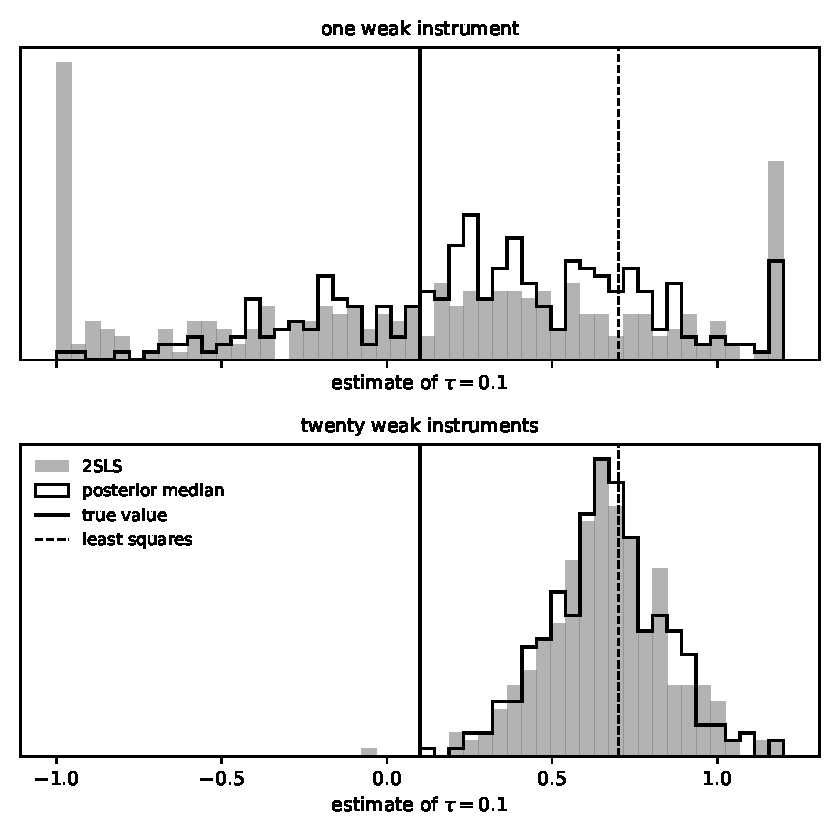
\includegraphics[width=\linewidth]{fig_weakiv.pdf}
\caption{Weak instruments in the spirit of quarter of birth: one instrument (top) and twenty (bottom), 300 data sets each. Gray: two stage least squares; black outline: posterior medians under the diffuse structural prior, computed exactly. The solid line is the truth $\tau = 0.1$, the dashed line the median least squares estimate. Estimates outside the plotted range are counted in the end bins.}
\label{fig:weakiv}
\end{figure}

\section{Many instruments and the horseshoe}\label{iv:sec:many}

In finite samples with many instruments\index{many instruments|textbf}, the fitted treatment inherits first stage error correlated with the structural error, even when the true first stage is zero, biasing two stage least squares\index{two stage least squares}\index{two stage least squares!bias toward least squares|textbf} toward least squares. Shrinking the first stage reduces this overfitting. Belloni, Chen, Chernozhukov and Hansen (2012) used the lasso; a horseshoe first stage\index{horseshoe prior!for many instruments|textbf}\index{horseshoe prior} leaves strong coefficients almost untouched and pulls weak ones to zero, avoiding the lasso's constant shrinkage of strong instruments. It is not a cure for weakness\index{weak instrument!and the horseshoe|textbf}. With a zero first stage, and approximately with a weak one, $T = u_T$. Write the structural outcome equation as $Y = \tau T + e$, where $e = u_Y - \tau u_T$ has standard deviation $\sigma_e$ and correlation $\rho$ with $u_T$, whose standard deviation is $\sigma_T$. Then $Y = (\tau + \rho\sigma_e/\sigma_T)\,T + w$ with $w$ uncorrelated with $T$ (independent under joint normality), so the data identify only the least squares slope, and the prior decides where $\tau$ sits along the ridge on which that slope is fixed. A prior that lets the first stage be near zero lets the posterior spread along the ridge; one that insists on a strong first stage, as a flat prior on twenty coefficients does, holds it near two stage least squares.

Table~\ref{tab:ivmany} compares two stage least squares and three first stage priors on six designs with twenty instruments, 1,000 data sets each, otherwise as in Figure~\ref{fig:weakiv}. The concentration parameter $c$ is 1.8, 20 or 135, carried by $s = 3$ of the instruments or spread over all twenty, each active instrument having first stage coefficient $\sqrt{c/(ns)}$. The weak design of that figure is $c = 1.8$ over twenty instruments, and the sparse design discussed below has $c = 135$ on three instruments with coefficient 0.15 and seventeen at zero. The hierarchical normal prior, in the spirit of Chamberlain and Imbens (2004), gives the twenty coefficients a common normal distribution whose variance has an inverse gamma prior with shape 1 and scale $10^{-4}$; the horseshoe gives each coefficient its own half Cauchy local scale under a half Cauchy global scale $\gscale$, both with unit scale. Neither prior is scaled by the error variance, and both keep the $N(0, 10^4)$ priors on $\tau$ and the controls and the prior on $\Sigma$ of Section~\ref{iv:sec:weak}. Both are fitted by the blocked Gibbs sampler described below, four chains of 4{,}000 iterations with the first 1{,}000 discarded, rerun at 16{,}000 with 4{,}000 discarded when the split R-hat of $\tau$ exceeds 1.01, and the diffuse prior is computed exactly as before.

\begin{table}[ht]
\centering
\caption{Twenty instruments, 1,000 data sets per design, $n = 2{,}000$, $\tau = 0.1$ and error correlation 0.6. The concentration parameter $c$ is carried by $s$ active instruments, each with first stage coefficient $\sqrt{c/(ns)}$; the weak design of the text is $c = 1.8$ with $s = 20$, the sparse design $c = 135$ with $s = 3$. For two stage least squares the median estimate over data sets; for each first stage prior the median over data sets of the posterior median, the share of equal tailed 90\% intervals that cover the truth, and the median interval length. The Monte Carlo standard error of a coverage near 90\% is about one point.}
\label{tab:ivmany}
\small
\setlength{\tabcolsep}{4pt}
\begin{tabular}{lcccccc}
\toprule
& \multicolumn{3}{c}{Three active, $s = 3$} & \multicolumn{3}{c}{Twenty active, $s = 20$} \\
\cmidrule(lr){2-4}\cmidrule(lr){5-7}
First stage prior & Median & Coverage & Length & Median & Coverage & Length \\
\midrule
\multicolumn{7}{@{}l}{\textit{Concentration $c = 1.8$}} \\
Two stage least squares & 0.66 &  &  & 0.64 &  &  \\
Diffuse, exact & 0.66 & 10\% & 0.59 & 0.64 & 9\% & 0.59 \\
Hierarchical normal & 0.59 & 98\% & 3.09 & 0.56 & 98\% & 3.06 \\
Horseshoe & 0.62 & 99\% & 5.54 & 0.59 & 99\% & 5.54 \\
\midrule
\multicolumn{7}{@{}l}{\textit{Concentration $c = 20$}} \\
Two stage least squares & 0.39 &  &  & 0.40 &  &  \\
Diffuse, exact & 0.37 & 40\% & 0.45 & 0.38 & 39\% & 0.45 \\
Hierarchical normal & $-0.07$ & 91\% & 1.77 & $-0.05$ & 91\% & 1.75 \\
Horseshoe & 0.08 & 92\% & 1.23 & 0.11 & 95\% & 1.76 \\
\midrule
\multicolumn{7}{@{}l}{\textit{Concentration $c = 135$}} \\
Two stage least squares & 0.17 &  &  & 0.17 &  &  \\
Diffuse, exact & 0.17 & 77\% & 0.25 & 0.17 & 76\% & 0.25 \\
Hierarchical normal & 0.08 & 88\% & 0.32 & 0.08 & 89\% & 0.32 \\
Horseshoe & 0.10 & 89\% & 0.30 & 0.10 & 90\% & 0.31 \\
\bottomrule
\end{tabular}
\end{table}


In the weak design the diffuse prior is again confident and wrong. Both shrinkage priors gain coverage by widening the intervals, with medians little closer to the truth than two stage least squares: the posterior has learned that the instruments are weak, not where $\tau$ is. In the sparse design the first stage is strong in total, yet two stage least squares and the diffuse posterior are still pulled toward least squares. The hierarchical normal prior and the horseshoe bring the medians toward the truth and improve the coverage, with intervals a little longer. This is the design in which the horseshoe's ability to keep a few strong coefficients while zeroing the rest should matter most, and it gains modestly for $\tau$: its posterior median has root mean squared error 0.094 against 0.105 for the hierarchical normal prior and mean error $-0.010$ against $-0.027$. It also estimates the first stage better, with half the error on the seventeen inactive instruments (root mean squared error 0.008 against 0.016). The larger gain comes at $c = 20$. With three and with twenty active instruments its posterior median has mean error $-0.07$ and $-0.04$ against $-0.22$ and $-0.19$ for the hierarchical prior, root mean squared error 0.34 and 0.37 against 0.46 and 0.46, and its intervals cover 0.922 and 0.945 against 0.908 and 0.906, with three active instruments on a shorter interval, 1.23 against 1.77. The samplers mixed: in the weak design the largest split R-hat over data sets was \ivhwhierrhat\ for the hierarchical prior and \ivhwhsrhat\ for the horseshoe, with \ivhwhiersh\ and \ivhwhssh\ of runs below 1.01 after the longer rerun that about 3 percent of them needed, and in the sparse design \ivhshierrhat\ and \ivhsrhat. At $c = 20$ the largest values reached 1.17, 5 to 8 percent of runs needed the longer chains, and at most 0.6 percent stayed above 1.01.

The structural model treats both stages jointly, its bivariate error $(e_1, e_2)$ being $(u_T, e)$ above, with a correlation $\rho$ that measures the endogeneity. Gibbs sampling for it is easy to write and easy to get wrong. The natural sampler alternates the structural coefficients, first stage coefficients and $\Sigma$, each conditional on the others. On the ridge each block is pinned by the others, and the sampler crawls. On the Card data of Section~\ref{iv:sec:card}, four chains of 6{,}000 iterations from different starting values gave a split R-hat of \ivchcardoldrhat\ for $\tau$ and an effective sample size of \ivchcardoldess\ from the 20{,}000 draws kept, with lag one autocorrelation \ivchcardoldlag; a typical step moved $\tau$ by \ivchcardoldstep, against a posterior standard deviation of \ivchcardsd. On the first 20 data sets of the one instrument design, runs of 1{,}200 iterations gave intervals of median length \ivcholdlen\ that covered the truth in \ivcholdcov\ of data sets, where the exact posterior gives \ivchexactlen\ and \ivchexactcov, and runs of 20{,}000 iterations still gave only \ivcholdlonglen\ and \ivcholdlongcov. Drawing $\tau$ in one block with the coefficient of the regression of $e_2$ on $e_1$ lets the sampler move along the ridge: on the same data sets its posterior medians differ from the exact ones by \ivchblockdiff\ at the median. The samplers behind Table~\ref{tab:ivmany} and the right panel of Figure~\ref{fig:card} are blocked, with the shrinkage scales of the first stage updated by their own conditional step. The posterior for the error correlation reports how much endogeneity the data see, and an analyst with many candidate instruments should report which ones the posterior keeps, since a design that rests on one or two of them is a different design from one that rests on twenty.

\section[Worked example: college proximity]{Worked example: college proximity and the return to schooling}\label{iv:sec:card}

Card\index{Card, David|see{college proximity instrument}} (1995) asked whether growing up near a four year college raises schooling and, through it, earnings. The data are the 1976 wave of the National Longitudinal Survey of Young Men, \ivcardn\ men with wages, schooling and an indicator of a four year college in the local labour market in 1966. We follow the textbook specification of Wooldridge (2020, Example 15.4), which treats experience as exogenous; Card also instruments experience with age. The instrument is proximity\index{college proximity instrument|textbf}; the controls are experience and its square, race, residence in a metropolitan area and in the South in 1976, metropolitan residence in 1966, and region of residence in 1966. The motivating worry is ability bias: men with more schooling may have earned more anyway.

Least squares gives a return of \ivcardols\ per year of schooling\index{college proximity instrument!return to schooling|textbf} (standard error \ivcardolsse). The first stage coefficient of proximity on schooling is \ivcardfs\ years (standard error \ivcardfsse), a first stage $F$ statistic of \ivcardF, just above the conventional threshold of 10. Two stage least squares gives \ivcardtsls\ (standard error \ivcardtslsse), larger than least squares, which surprised many: if ability bias pushes least squares up, the instrument should pull the estimate down. The usual explanations are unusually high returns among the compliers, men kept in school by a nearby college, and measurement error\index{measurement error|textbf} in schooling, which biases least squares toward zero. Schooling takes many values, so the instrumental variable estimate is not the binary complier effect of the theorem but the average causal response\index{average causal response|textbf} of Angrist and Imbens (1995), a weighted average of the effects of an extra year of schooling at each margin the instrument moves, and the complier share of Section~\ref{iv:sec:late} has no direct analogue.

Two Bayesian analyses show how much the parametrization matters at this strength of instrument. The first places flat priors on the coefficients of proximity and the controls in the reduced form wage and schooling equations and the prior $|\Omega|^{-3/2}$ on the covariance $\Omega$ of their errors, and takes the return as the ratio of the two proximity coefficients: posterior median \ivcardrfmed, 90\% interval from \ivcardrflo\ to \ivcardrfhi, and posterior probability \ivcardrfpgt\ that the return exceeds least squares. That interval agrees, to within simulation error, with the 90\% Anderson and Rubin confidence set of Section~\ref{iv:sec:weak}, which runs from 0.044 to 0.249. The second is the structural posterior of Section~\ref{iv:sec:weak}, computed exactly: median \ivcardsmed, 90\% interval from \ivcardslo\ to \ivcardshi, and probability \ivcardspgt\ of exceeding least squares. Figure~\ref{fig:card} shows it. The two agree on the centre and on the comparison with least squares, and the structural posterior has the longer tails. With a first stage $F$ of \ivcardF\ the parametrization matters little; it is with a weak instrument, as in Figure~\ref{fig:weakiv}, that the prior takes over.

\begin{figure}[htbp]
\centering
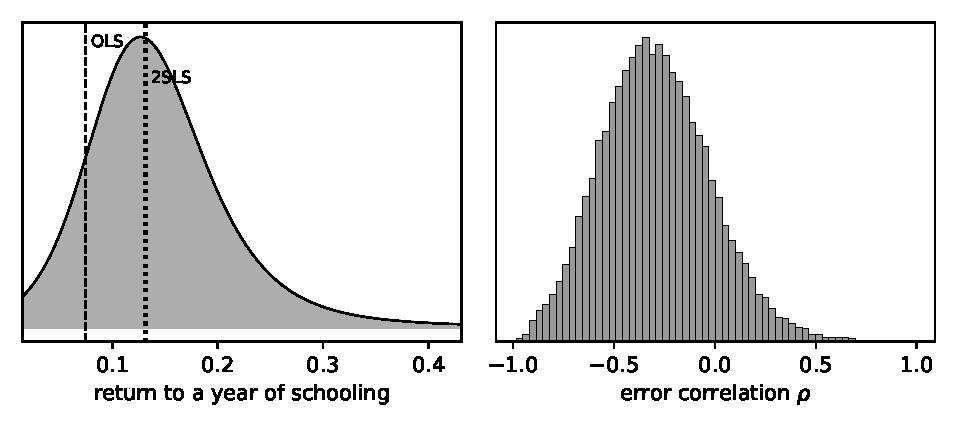
\includegraphics[width=\linewidth]{fig_card.pdf}
\caption{College proximity as an instrument for schooling (Card 1995). Left: exact posterior of the return to a year of schooling under the diffuse structural prior of Section~\ref{iv:sec:weak}, with the least squares (dashed) and two stage least squares (dotted) estimates. Right: posterior of the correlation between the errors of the schooling and wage equations, from the blocked Gibbs sampler of Section~\ref{iv:sec:many} (four chains of 11{,}000 iterations, the first 1{,}000 of each discarded; split R-hat \ivcardrhat\ and effective sample size \ivcardess\ for the return).}
\label{fig:card}
\end{figure}

The posterior of the error correlation has mean \ivcardrho, 90\% interval from \ivcardrholo\ to \ivcardrhohi, and probability \ivcardrhopneg\ of being negative. A negative correlation makes least squares too small, the direction that measurement error in schooling would produce, and the data lean that way, but they leave real probability on the positive correlation that ability bias implies. That is what comparing least squares with two stage least squares was trying to say, now with a probability attached.

\section{Instruments in unlikely places}\label{iv:sec:unlikely}

The search for instruments\index{instrumental variable!in unlikely places|textbf} has produced many ingenious and contested designs. A good instrument must move treatment for reasons unrelated to the outcome, so it is usually something nobody would think of as a cause of the outcome. Table~\ref{tab:unlikely} lists examples; most have drawn a critique of the assumption that made them clever.

\begin{table}[htbp]
\centering\scriptsize
\renewcommand{\arraystretch}{1.1}
\begin{tabular}{@{}L{1.0in}L{0.9in}L{0.95in}L{1.15in}@{}}
\toprule
Instrument & Treatment & Outcome & The worry \\
\midrule
Quarter of birth (Angrist and Krueger 1991) & years of schooling & earnings & weak first stage (Bound, Jaeger and Baker 1995); season of birth and family background (Buckles and Hungerman 2013) \\
Draft lottery number (Angrist 1990) & military service in Vietnam & civilian earnings & the lottery may change behaviour directly, through schooling to avoid service \\
Two first children of the same sex (Angrist and Evans 1998) & a third child & mother's labour supply & sex composition may affect costs directly \\
College nearby (Card 1995) & schooling & earnings & families choose where to live \\
Stormy weather at sea (Angrist, Graddy and Imbens 2000) & price of fish & quantity demanded & Wright's supply shifter again; few observations \\
Rainfall (Miguel, Satyanath and Sergenti 2004) & economic growth & civil conflict & rain may affect conflict directly (Sarsons 2015) \\
Settler mortality (Acemoglu, Johnson and Robinson 2001) & institutions & income per head & measurement of mortality (Albouy 2012) \\
Electoral cycles (Levitt 1997) & police numbers & crime & not significant once a coding error is corrected (McCrary 2002) \\
Streams that divide school districts (Hoxby 2000) & school choice & achievement & counting of streams (Rothstein 2007) \\
Randomly assigned judges (Kling 2006) & incarceration & later earnings & monotonicity across judges (Frandsen, Lefgren and Leslie 2023) \\
Genetic variants (Davey Smith and Ebrahim 2003) & an exposure such as alcohol & disease & pleiotropy (Section~\ref{iv:sec:mr}) \\
\bottomrule
\end{tabular}
\caption{Instruments in unlikely places. In each case the instrument is plausible precisely because it seems unrelated to the outcome, and most of the critiques question that.}
\label{tab:unlikely}
\end{table}



\paragraph{Quarter of birth.} Angrist and Krueger (1991) noticed that compulsory schooling laws require attendance until a birthday, usually the sixteenth, while school entry is by calendar year. Children born early in the year reach the leaving age with slightly less schooling than those born late, so quarter of birth\index{quarter of birth instrument|textbf} shifts schooling a little. Nobody believes season of birth affects earnings directly, which makes the instrument persuasive. But the first stage is tiny, and with many interactions of quarter of birth with state and year the instruments are individually very weak. Bound, Jaeger and Baker (1995) showed that two stage least squares with such instruments is biased toward least squares, and that randomly generated quarters of birth produced estimates and standard errors similar to the published ones.  Later work related season of birth to mothers' characteristics (Buckles and Hungerman 2013), so exclusion is not as safe as it looked either.

\paragraph{Same sex siblings.} Angrist and Evans (1998) used the fact that American parents whose first two children share a sex are more likely to have a third. A child's sex is as good as random, and it seems absurd that two daughters rather than a daughter and a son would affect a mother's employment except through family size. The design gives a credible local effect of a third child for families whose fertility responds to sex composition, a specific and perhaps unusual group of compliers.

\paragraph{Fish and weather.} Angrist, Graddy and Imbens (2000) used stormy weather to instrument the price of whiting in New York's Fulton fish market (Graddy 1995), repeating Wright's supply shifter: weather shifts supply, plausibly not demand. With only a few months of trading days, the design calls for uncertainty statements that hold in small samples.

\section{Nonparametric instruments}\label{iv:sec:nonpar}

With continuous treatment and a nonlinear structural function\index{nonparametric instrumental variables|textbf},
\[
Y = f(T) + \varepsilon, \qquad \E(\varepsilon \mid Z) = 0,
\]
and $f$ solves the integral equation
\[
\E(Y \mid Z) = \E\{f(T) \mid Z\} = (\mathcal{K} f)(Z),
\]
where $\mathcal{K}$ is the conditional expectation operator from functions of $T$ to functions of $Z$. The equation identifies $f$ only if $\mathcal{K}$ is injective, the completeness condition of Newey and Powell (2003): the only function $h$ with $\E\{h(T) \mid Z\} = 0$ is $h = 0$. Even then inverting $\mathcal{K}$ is ill posed\index{ill posed inverse problem|textbf}: $\mathcal{K}$ is typically compact, its singular values accumulate at zero, and small errors in $\E(Y \mid Z)$ produce large errors in $f$.

Kernel instrumental variables\index{kernel instrumental variable|textbf}, introduced by Singh, Sahani and Gretton in 2019, represent $f$ in a reproducing kernel Hilbert space and estimate $\mathcal{K}$ by kernel ridge regression of features of $T$ on features of $Z$; the second stage regresses $Y$ on the estimated conditional mean embedding. The first stage is a vector valued regression and the second a scalar one, with theory resting on source conditions that measure the smoothness of $f$ relative to $\mathcal{K}$.

\paragraph{Source conditions, priors and saturation.}  The H\"older source condition of order $r$, that $f = \mathcal{C}^{r} g$ with $\|g\| < \infty$ for the covariance operator $\mathcal{C}$, says that $f$ lies in the Cameron Martin space of the Gaussian prior with covariance $\mathcal{C}^{2r}$ (a prior that exists when $\mathcal{C}^{2r}$ has finite trace): in the eigenbasis of $\mathcal{C}$, with eigenvalues $s_k$, the Cameron Martin norm $\sum_k f_k^2/s_k^{2r}$ is $\|g\|^2$ (Exercise~\ref{ex:ch10:5}). When $\mathcal{C}$ has infinite rank, draws from that prior fall outside the space almost surely, since their norm is a sum of infinitely many squared independent standard normals. With fixed scale $c$ the posterior still contracts, but more slowly; attaining the rate below requires $c$ to depend on $n$. In the sequence model $y_k = f_k + n^{-1/2}\xi_k$, with $\xi_k$ independent standard normal, the consequences take a few lines:
\begin{itemize}
\item Ridge regression with penalty $\alpha$ multiplies $y_k$ by $s_k/(s_k + \alpha)$. That is the posterior mean under $f_k \sim N(0, cs_k)$ with $\alpha = 1/(nc)$, so the prior implicit in ridge has covariance proportional to $\mathcal{C}$, the case $r = 1/2$ of the reading above.
\item The prior with covariance $c\,\mathcal{C}^{2r}$ multiplies $y_k$ by $s_k^{2r}/(s_k^{2r} + a)$ with $a = 1/(nc)$. Under the source condition of order $r$, its squared bias is at most $a\|g\|^2/4$, since $as_k^{r}/(s_k^{2r} + a) \le \sqrt{a}/2$. With $s_k$ of order $k^{-b}$ and $2rb > 1$, the variance of the posterior mean and the posterior spread are both of order $a^{-1/(2rb)}/n$. Balancing gives posterior expected squared error, averaged over the data, of order $n^{-2rb/(2rb+1)}$, with $a$ of that order and $c$ of order $n^{-1/(2rb+1)}$. The contraction rate in norm is its square root, $\varepsilon_n = n^{-rb/(2rb+1)}$: writing $f_0$ for the truth, Markov's inequality gives $\E_{f_0}\Pi(\|f - f_0\| > M_n\varepsilon_n \mid y) \to 0$ for every $M_n \to \infty$, uniformly over $\|g\| \le R$ for fixed $R$. For $r \le 1$ ridge reaches the same order of worst case mean squared error in this model at the best $\alpha$ (squared bias of order $\alpha^{2r}$ from Exercise~\ref{ex:ch10:6}, variance of order $\alpha^{-1/b}/n$). With random design, taking $\mathcal{C}$ to be the kernel integral operator on $L^2$ of the law of $T$, Theorem 1 of Caponnetto and De Vito (2007) gives the same power for the squared prediction error of kernel ridge when $1/2 < r \le 1$ and $b > 1$, under a bounded kernel and moment conditions on the noise; at $r = 1/2$ their upper bound is $(\log n/n)^{b/(b+1)}$, larger by a logarithmic factor. 
\item Saturation, ridge regression ceasing to improve once the source condition exceeds a threshold, belongs to the fixed prior. With covariance proportional to $\mathcal{C}^{2r_0}$ and truth of order $r$, the same calculation gives squared bias of order $a^{2\min\{r/(2r_0),\,1\}}$ while the variance does not depend on $r$, so the rate stops improving at $r = 2r_0$. Ridge has $r_0 = 1/2$ and stops at $r = 1$ (Exercise~\ref{ex:ch10:6}). A Gaussian prior matched to the smoothness, $r_0 = r$, is below its ceiling for every $r$, but it has to be told $r$.
\item For unknown $r$ we propose a global local prior on a finite expansion: $f = \sum_{k=1}^m f_k\phi_k$, with $\phi_k$ the eigenfunctions of $\mathcal{C}$ and horseshoe scales on the coefficients, $f_k \mid \lambda_k, \gscale \sim N(0, \lambda_k^2\gscale^2)$, as in Chapter~\ref{ch:horseshoe}. The cutoff $m$ is part of the prior: infinitely many coefficients that are independent and identically distributed given $\gscale$ have $\sum_k f_k^2 = \infty$ almost surely, so without it the prior does not live on the space of the source condition. With $m$ growing in $n$, and eigenvalues in decreasing order, a truth of order $r$ has squared truncation error at most $s_{m+1}^{2r}\|g\|^2$. We expect the prior to adapt without saturating, and we have no proof and no rule for choosing $m$. The expectation rests on where the ceiling comes from: in Exercise~\ref{ex:ch10:6} it is the bias on the largest coordinates, of order $\alpha$ for ridge, while the horseshoe's tails shrink a large $y_k$ by only about $2/(ny_k)$ (Chapter~\ref{ch:horseshoe}). The contraction results we know for the horseshoe, such as van der Pas, Szab\'o and van der Vaart (2017a), concern nearly black vectors, not source sets, so whether it attains the rate for every $r$ remains open.
\end{itemize}
With an operator in the model the coordinates are observed through its singular values, which slow the rate. Knapik, van der Vaart and van Zanten (2011) carry out the calculation for Gaussian priors: with $\mathcal{K}$ known, diagonal in the eigenbasis of $\mathcal{C}$, with singular values of order $k^{-p}$, and with $c$ of order $n^{-1/(2rb+2p+1)}$, the rate in norm is $n^{-rb/(2rb+2p+1)}$, and $p = 0$ returns the rate above. This is a benchmark, since in nonparametric instruments $\mathcal{K}$ is estimated and its error needs control of its own. A rate is also not coverage: the same paper shows that credible sets under a prior smoother than the truth can have frequentist coverage tending to zero. Knapik, Szab\'o, van der Vaart and van Zanten (2016) show that empirical and hierarchical Bayes over the regularity of a Gaussian prior adapt in mildly ill posed problems. The horseshoe would have to do at least as well to justify its place.

\paragraph{Scalability.} Kernel methods scale as the cube of the sample size, prohibitive for instruments in large administrative data sets. Random features, Nystr\"om approximation and conjugate gradient solvers cut the cost, and the first two are themselves priors. With $m$ random features $\varphi_j$, the function $f = \sum_j \beta_j\varphi_j$ with $\beta_j$ independent $N(0, 1/m)$ has a Gaussian prior of dimension $m$ and covariance $m^{-1}\sum_j \varphi_j(t)\varphi_j(t')$. Nystr\"om at $m$ points $v$ replaces the kernel $\kappa$ by $\kappa(t, v)\kappa(v, v)^{-1}\kappa(v, t')$, the covariance of $\E\{f(t) \mid f(v)\}$ under the Gaussian process prior with kernel $\kappa$, a prior covariance of rank $m$. Either way the intervals are those of the low rank prior, and they should not be read as those of the full kernel. The global local prior is conditionally Gaussian: given its scales, an EM step or a Gibbs sweep is a weighted ridge regression, at about the cost of one kernel ridge regression. How many such steps a fit takes is an open question for us.

\section{Mendelian randomization}\label{iv:sec:mr}

Within families, genetic variants are assigned at conception almost randomly; those that affect an exposure can serve as instruments for it. This is Mendelian randomization\index{Mendelian randomization|textbf}, proposed by Katan (1986) and developed by Davey Smith and Ebrahim (2003).

Fisher's constitutional hypothesis (Chapter~\ref{ch:smoking}) was that genes caused both smoking and lung cancer. Mendelian randomization turns it around: a gene that affects smoking quantity, and lung cancer only through smoking, is an instrument for smoking. Variants in the nicotinic receptor gene cluster on chromosome 15, which are associated with the number of cigarettes smoked per day (Thorgeirsson et al. 2008), have been used in this way to study the effects of smoking heaviness.

Exclusion is the weak point. A variant may affect the outcome through pathways other than the exposure, which geneticists call horizontal pleiotropy\index{Mendelian randomization!pleiotropy|textbf}. With many variants, MR Egger regression (Bowden, Davey Smith and Burgess 2015), which needs the direct effects to be independent of the variants' effects on the exposure, and weighted median estimators (Bowden, Davey Smith, Haycock and Burgess 2016), which need more than half of the weight to come from valid variants, relax the requirement that every variant be valid. A Bayesian treatment puts a sparsity prior on variants' direct effects, most near zero and a few not. Provided most variants are valid, a horseshoe\index{horseshoe prior} lets that majority locate the effect; variants whose direct effects escape shrinkage look invalid. The horseshoe gives no exact zeros, so a posterior probability that a variant is valid needs a prior with a point mass at zero.

\section{Instruments as accounting}\label{iv:sec:accounting}

Two valid instruments\index{instrumental variable!accounting view|textbf} for the same treatment can give different local average treatment effects\index{local average treatment effect}, both correct, because each defines its own compliers. On the accounting view\index{accounting identity!and instruments|textbf} the object of inference is the structural model: in the binary case, the joint law of potential treatments and outcomes. The local effect\index{local average treatment effect!as accounting|textbf} is one accounting of it, over that instrument's compliers. A model of how effects and compliance vary with covariates can compute the local effect for any instrument and the average effect for any population. Without one, each instrument answers only its own question.

College proximity moves men who would otherwise have stopped at the end of secondary school; quarter of birth moves those who leave at the earliest legal age. Both instrument schooling, yet their compliers can have different returns even if both exclusion restrictions hold. A joint model of returns and compliance computes each local effect by averaging the same conditional effect with different weights, provided compliance carries no information about the effect once covariates are fixed. Population weights give the population average. Where compliers cover only part of the covariate space, this average relies on extrapolation; posterior width there comes from the prior on how effects vary with covariates, so it should be reported under more than one such prior.

Report the local effect and its compliers, and, when a model is fitted, the average for the population of interest with its wider interval, showing how much comes from data and how much from the model.

\section{In practice}

\paragraph{The target.} Each posterior draw gives $\tau^{(s)}$, directly or as $\pi_Y^{(s)}/\pi_T^{(s)}$; the complier effect from the outcome models of the imputed strata; or $f^{(s)}$ from the eigenbasis coefficients. Averaging $f^{(s)}(t) - f^{(s)}(t')$ over any law of $(t, t')$ gives a policy effect, again by accounting.

\paragraph{What the analyst does differently.} An analyst with an instrument should state the exclusion restriction as a scientific claim and say who the compliers are, since the local effect describes no one else. She should report the first stage with its posterior, not only an $F$ statistic, and the posterior for the error correlation, since it reports the endogeneity the design exists to address. With many instruments she should shrink the first stage and report which instruments the posterior keeps (Section~\ref{iv:sec:many}). She should state the prior on the error covariance and report the posterior under more than one prior, because with one weak instrument the scale of that prior moved the coverage of nominal 90\% intervals from \ivscaledefcov\ to \ivscalehundcov\ (Section~\ref{iv:sec:weak}). She should also run more than one chain from different starting values, because a one at a time Gibbs sampler crawls on the ridge (Section~\ref{iv:sec:many}).

\paragraph{Against DML.} Double machine learning has an instrumental variable score (Chernozhukov et al. 2018; Table~\ref{tab:dml:scores}), and for a single strong instrument in a linear model it and two stage least squares are adequate and cheaper; the Bayesian answer then agrees with two stage least squares, as in the Card data, and costs more, so the case for it lies elsewhere. We did not run the score, on the Card data or on the designs of Section~\ref{iv:sec:weak}, so what the runs show concerns two stage least squares and the posteriors. With one weak instrument two stage least squares is erratic, while the structural and reduced form posteriors report the weakness as wide intervals. With twenty weak instruments no method we ran recovers the truth: two stage least squares and the diffuse structural posterior sit next to least squares, and the shrunk first stages of Table~\ref{tab:ivmany} cover the truth by being wide, not by being right. With a nonlinear structural function the ill posed inverse needs a prior matched to the unknown smoothness, and the global local prior of Section~\ref{iv:sec:nonpar} is proposed for that purpose; we have not tested it here. The limit on our side is the weight a weak instrument puts on the prior for the error covariance: the Bayesian analyst must state that prior and show what changes when it does.

\section*{Notes}



The chapter assumes monotonicity; Balke and Pearl (1997) bound the average effect without it, by linear programming over response types, as in Chapter~\ref{ch:tianpearl}.

\begin{exercises}
\item\label{ex:ch10:1} Derive the bias of least squares in the linear model and check it against the simulated mean of 1.89 in the design of Figure~\ref{fig:iv}.
\item\label{ex:ch10:2} Show that the Wald ratio with one instrument has no finite mean when the reduced form and first stage coefficient estimates are jointly normal, the first stage estimate has positive variance and the correlation between the two estimates is below one in absolute value.
\item\label{ex:ch10:3} Prove the theorem of Section~\ref{iv:sec:late}, and show where each assumption is used.
\item\label{ex:ch10:4} Write the data augmentation sampler for the Imbens and Rubin model with normal outcomes in each stratum.
\item\label{ex:ch10:5} Show that the H\"older source condition $f = \mathcal{C}^{r}g$ with $\|g\| < \infty$ says that $f$ lies in the Cameron Martin space of the Gaussian prior with covariance $\mathcal{C}^{2r}$, assuming $\mathcal{C}^{2r}$ has finite trace.
\item\label{ex:ch10:6} Explain why ridge regression saturates at source condition $r = 1$.
\item\label{ex:iv:wright} In Wright's market with demand $q = a - bp + u_d$ and supply $q = c + dp + ew + u_s$, derive the probability limit of the least squares slope of $q$ on $p$ and show that it is a weighted average of $-b$ and $d$. Check the value against Figure~\ref{fig:wright}, which shows a single sample of 200 markets.
\item\label{ex:iv:card} Using \texttt{iv\_card.py} and \texttt{iv\_weak2.py}, add the father's and mother's education to the controls in the Card example, which loses observations. How do two stage least squares, the reduced form posterior and the exact structural posterior change, and why?
\item\label{ex:iv:qob} Explain why replacing true quarters of birth by random numbers would, with many interactions, give two stage least squares estimates close to least squares. What does the reduced form posterior give for a single random instrument?
\item\label{ex:iv:samesex} In the same sex design, describe the compliers. Using the accounting identity, explain why the local effect of a third child need not equal the average effect of a third child among all mothers of two.
\item\label{ex:iv:iwscale} In the structural model of Section~\ref{iv:sec:weak} take $\pi = 0$ and no controls. Show that the likelihood depends on $(\tau, \Sigma)$ only through the covariance matrix $\Omega$ of $(T, Y)$, that for each $\tau$ exactly one $\Sigma$ gives a fixed $\Omega$, and that $|\Sigma| = |\Omega|$ along the resulting curve. Show that along it, with $\Omega$ at the sample covariance matrix, the inverse Wishart prior with scale $c\,\mathrm{diag}(\Omega_{11}, \Omega_{22})$ is proportional to $\exp\{-c\,\Omega_{11}^2(\tau - b)^2/(2|\Omega|)\}$, where $b = \Omega_{12}/\Omega_{11}$ is the least squares slope. In the design of Figure~\ref{fig:weakiv}, what lengths of 90\% intervals does this predict for $c = 0.01$, 0.1, 1 and 10, and why are the lengths reported in Section~\ref{iv:sec:weak} shorter?
\item\label{ex:iv:flatK} Let the first stage have $K$ instruments, a fixed error variance $\sigma_T^2$ and a flat prior on $\pi$. Show that the concentration parameter $\mu^2 = \pi^\top Z^\top Z\pi/\sigma_T^2$ then has a prior density proportional to $(\mu^2)^{K/2 - 1}$. Compare $K = 1$ with $K = 20$, and use the comparison to explain the coverage of the diffuse structural posterior with one and with twenty weak instruments in Section~\ref{iv:sec:weak}.
\end{exercises}

\chapter{Bounds and Sensitivity}\label{ch:tianpearl}

\begin{tcolorbox}[colback=gray!6,colframe=gray!50,title=In brief,fonttitle=\normalfont\itshape,coltitle=black,colbacktitle=gray!15,boxrule=0.4pt,arc=1pt]
The probabilities that a treatment was necessary, sufficient, or both depend on the joint law of potential outcomes and are bounded rather than identified. Combining experimental and observational data narrows the bounds, and a Bayesian posterior over the position inside them gives a court the probability it actually needs. The second half of the chapter turns to unmeasured confounding: Cornfield's inequality, Rosenbaum's parameter and the E value say how strong a hidden confounder must be to overturn a result, and a prior on the confounding parameters turns that threshold into a posterior probability that the effect is positive.
\end{tcolorbox}

A court hearing a claim against a tobacco company does not ask whether smoking raises the risk of lung cancer in the population. It asks whether this plaintiff's cancer was caused by smoking: a question about the joint behaviour of two potential outcomes for one person. Pearl\index{Pearl, Judea!probabilities of causation|textbf} (1999) defined the probabilities of necessity, sufficiency and both. Tian and Pearl (2000) showed that experimental and observational data bound them but, without further assumptions such as monotonicity, do not point identify them.

\section{Three probabilities of causation}

Let $X$ be a binary exposure and $Y$ a binary outcome. From Section~\ref{sec:sensitivity} on, treatment is $T$ and covariates are $X$; Cornfield's inequality and the E value use exposure $E$ and disease $D$. Write $y_x$ for $Y(x) = 1$, $y'_x$ for $Y(x) = 0$, $x$ for $X = 1$ and $x'$ for $X = 0$.

\begin{definition}[Probabilities of causation]
\begin{align*}
\PN &= \Prob(y'_{x'} \mid x, y), && \text{probability of necessity,}\\
\PS &= \Prob(y_x \mid x', y'), && \text{probability of sufficiency,}\\
\PNS &= \Prob(y_x, y'_{x'}), && \text{probability of necessity and sufficiency.}
\end{align*}
\end{definition}

$\PN$ asks: what fraction of the exposed who developed the outcome would not have developed it without exposure\index{probability of necessity|textbf}\index{PN|see{probability of necessity}}? $\PS$ asks the reverse: what fraction of the unexposed without the outcome would have developed it if exposed\index{probability of sufficiency|textbf}? $\PNS$ is the probability that a random person is one for whom exposure makes the difference both ways\index{probability of necessity and sufficiency|textbf}\index{PNS|see{probability of necessity and sufficiency}}.

A court asks $\PN$, because the plaintiff was exposed and fell ill and the issue is whether the exposure was needed. A regulator deciding whether to permit an exposure asks $\PS$, because the people at issue are not yet exposed. A company choosing whom to target with an incentive asks $\PNS$ whenever a customer put off by the incentive costs it a different amount from what a converted customer earns (Section~\ref{sec:decisions}). None of the three is an average treatment effect. The average effect $\Prob(y_x) - \Prob(y_{x'})$ compares two margins; the probabilities of causation\index{probabilities of causation|textbf} ask how the two potential outcomes of one person sit together, the coupling of Section~\ref{sec:ot}. Two populations with the same margins can differ in that respect, one in which exposure harms some and protects others, another in which it only harms, and the probabilities of causation differ between them while every average agrees.

For binary outcomes the coupling is a single number once the two margins are known. $\PN$ and $\PS$ also depend on who chose exposure, through the joint law of $(X, Y(0), Y(1))$, which leaves two such numbers once the experimental and observational margins are known. The data inform the margins, and the numbers that fix the coupling are seen by no one, because no person is observed both exposed and unexposed.

\section{Bounds from experimental and observational data}

\paragraph{Experimental data alone.} A randomized experiment gives $\Prob(y_x)$ and $\Prob(y_{x'})$. The joint law of $(Y(0), Y(1))$ is a $2 \times 2$ table with these margins and one free parameter.

\begin{theorem}[Tian and Pearl]
From experimental data alone\index{probabilities of causation!bounds on|textbf},
\[
\max\{0,\ \Prob(y_x) - \Prob(y_{x'})\} \leq \PNS \leq \min\{\Prob(y_x),\ \Prob(y'_{x'})\}.
\]
\end{theorem}

\begin{proof}
Write $p_{ab} = \Prob\{Y(1) = a, Y(0) = b\}$. Then $\PNS = p_{10} = \Prob(y_x) - \Prob(y_{x'}) + p_{01}$, so nonnegativity gives the lower bound. Also $p_{10} \leq \Prob(y_x)$ and $p_{10} \leq \Prob(y'_{x'})$, giving the upper bound.
\end{proof}

When $\Prob(y_x) \geq \Prob(y_{x'})$, the lower bound is attained when exposure prevents the outcome in no one, $p_{01} = 0$: monotonicity. Then $\PNS = \Prob(y_x) - \Prob(y_{x'})$, the risk difference. When the order is reversed the lower bound is zero, and the margins themselves rule monotonicity out. Section~\ref{gr:sec:margins} derives the same bounds as Fr\'echet bounds on the fraction helped in the urn of a randomized experiment, and says which other quantities the margins identify.

\paragraph{Combining experimental and observational data.} Tian and Pearl's deeper result is that observational data, revealing who chose exposure and what followed, narrow the bounds\index{Tian and Pearl bounds|textbf} further.

\begin{theorem}[Tian and Pearl]
With both experimental quantities $\Prob(y_x), \Prob(y_{x'})$ and observational quantities $\Prob(x, y)$, $\Prob(x, y')$, $\Prob(x', y)$, $\Prob(x', y')$, measured on the same population, with $Y = Y(X)$ in the observational data, and writing $\Prob(y)$ for the observational outcome rate,
\[
\max\left\{0,\ \frac{\Prob(y) - \Prob(y_{x'})}{\Prob(x, y)}\right\} \leq \PN \leq \min\left\{1,\ \frac{\Prob(y'_{x'}) - \Prob(x', y')}{\Prob(x, y)}\right\},
\]
and $\PNS$ lies between
\[
\max\{0,\ \Prob(y_x) - \Prob(y_{x'}),\ \Prob(y) - \Prob(y_{x'}),\ \Prob(y_x) - \Prob(y)\}
\]
and
\begin{multline*}
\min\bigl\{\Prob(y_x),\ \Prob(y'_{x'}),\ \Prob(x, y) + \Prob(x', y'),\\
\Prob(y_x) - \Prob(y_{x'}) + \Prob(x, y') + \Prob(x', y)\bigr\}.
\end{multline*}
\end{theorem}

Tian and Pearl (2000) prove it by linear programming: the joint law of $(X, Y(0), Y(1))$ has eight cells, the data fix several linear combinations, and the bounds are the extremes of $\PN$ or $\PNS$ over the remaining polytope (Appendix~\ref{app:graphs} sketches the program).

The bound on $\PN$ follows in a few lines from a single cell. Let $q_{111} = \Prob\{X = 1, Y(1) = 1, Y(0) = 1\}$, the exposed who fall ill and would have fallen ill anyway, and let $r = \Prob(y_{x'}) - \Prob(x', y)$, the share who are exposed and have $Y(0) = 1$, since the unexposed show $Y(0)$. The exposed who fall ill have $Y(1) = 1$, so $\PN = 1 - q_{111}/\Prob(x, y)$ when $\Prob(x, y) > 0$. The exposed with $Y(0) = 1$ either fall ill under exposure, and are counted in $q_{111}$, or are among the $\Prob(x, y')$ who stay well, so
\[
\max\{0,\ r - \Prob(x, y')\} \leq q_{111} \leq \min\{\Prob(x, y),\ r\}.
\]
The upper limit gives the lower bound on $\PN$ and the lower limit gives the upper bound.

The same argument with the cell $\Prob\{X = 0, Y(1) = 1, Y(0) = 0\}$ bounds the probability of sufficiency, for $\Prob(x', y') > 0$:
\[
\max\left\{0,\ \frac{\Prob(y_x) - \Prob(y)}{\Prob(x', y')}\right\} \leq \PS \leq \min\left\{1,\ \frac{\Prob(y_x) - \Prob(x, y)}{\Prob(x', y')}\right\}.
\]
Splitting the people exposure helps by whether they chose it gives $\PNS = \Prob(x, y)\,\PN + \Prob(x', y')\,\PS$, an identity every joint posterior draw of the three must satisfy. Under monotonicity, with margins that allow it, all three are identified without exogeneity (Tian and Pearl 2000), each at its lower bound: $\PNS = \Prob(y_x) - \Prob(y_{x'})$, $\PN = \{\Prob(y) - \Prob(y_{x'})\}/\Prob(x, y)$ and $\PS = \{\Prob(y_x) - \Prob(y)\}/\Prob(x', y')$.



\section{The Bayesian reading}

The bounds are what the data say; a Bayesian adds what the analyst believes about the rest.

This is not a departure from Pearl. Chapter 8 of \emph{Causality} (Pearl 2009) follows its linear programming bounds for noncompliance with finite sample inference by Gibbs sampling over response types, after Chickering and Pearl (1996), and shows how the posterior inside the bounds depends on the prior. We do the same for the probabilities of causation\index{probabilities of causation!Bayesian reading|textbf} of Pearl's Chapter 9.

Parametrize the joint law by its identified margins and an unidentified $u \in [0,1]$ locating $\PNS$ within its bounds:
\[
\PNS = \PNS_{\mathrm{lo}} + u(\PNS_{\mathrm{hi}} - \PNS_{\mathrm{lo}}),
\]
where the bounds $\PNS_{\mathrm{lo}}$ and $\PNS_{\mathrm{hi}}$ are functions of the identified margins. Place a prior on $u$, independent of the margins. As $n$ grows the posterior for the margins concentrates; the posterior for $u$ equals its prior.

\begin{proposition}\label{prop:partial}
In a partially identified model with identified parameter $\phi$ and unidentified parameter $\xi$, a priori independent, where the likelihood depends on $\phi$ alone, the posterior of $\phi$ concentrates at $\phi_0$ and $h$ is continuous in $\phi$, the posterior of $\tau = h(\phi, \xi)$ converges weakly as $n \to \infty$ to the law of $h(\phi_0, \xi)$ with $\xi$ drawn from its prior.
\end{proposition}

Appendix~\ref{app:theory} proves it, allowing $\xi$ to depend on $\phi$ a priori. Here $\phi$ holds the identified margins, $\xi = u$ and $\tau = \PNS$, so the limiting posterior is the prior on $u$ spread between the limiting bounds.

Figure~\ref{fig:pns} shows a hypothetical experiment with 500 units per arm, 150 events under exposure and 50 without, with uniform priors on the two arm risks and 20,000 posterior draws. The posteriors of the two bounds are centred near 0.20 and 0.30. We show two posteriors for $\PNS$: one with $u$ uniform, and one with $u \sim \mathrm{Beta}(1/2, 1/2)$, which puts most mass near the ends of the interval.

\begin{figure}[ht]
\centering
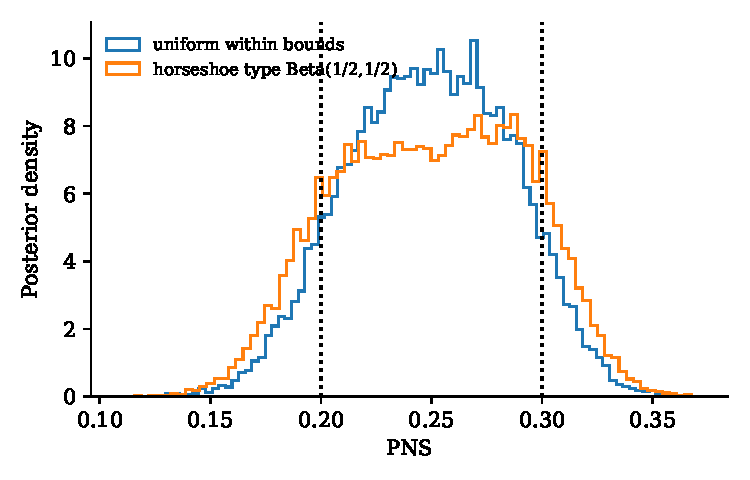
\includegraphics[width=\linewidth]{pns.pdf}
\caption{Posterior of $\PNS$ in a hypothetical experiment with 150 of 500 exposed and 50 of 500 unexposed developing the outcome, under two priors for its position within the bounds (dotted lines at the population bounds 0.20 and 0.30).}
\label{fig:pns}
\end{figure}

The $\mathrm{Beta}(1/2, 1/2)$ prior is the law of the horseshoe\index{horseshoe prior} shrinkage coefficient from Chapter~\ref{ch:horseshoe} at unit global scale. It favours two cases: exposure essentially never prevents the outcome and $\PNS$ is near the lower bound, or it has substantial effects in both directions and $\PNS$ is near the upper bound. Firm belief in monotonicity puts a point mass at $u = 0$ and recovers the risk difference.

The probabilities of causation also extend the accounting view. The average treatment effect is accounting over covariates; $\PNS$ is accounting over the unidentified coupling. Both are posterior functionals, but the second carries a prior no amount of data will overwhelm, and the honest report states it.

\section{Individual decisions}\label{sec:decisions}

Mueller, Li and Pearl (2022) used these bounds to choose whom to treat\index{individual decision|textbf}. A company offering customers an incentive wants to target those for whom it makes the difference, not those who would buy anyway or never buy. Within a covariate stratum, let $p_{10} = \PNS$ be the share the incentive converts and $p_{01}$ the share it deters. If a purchase earns $g$ and the incentive costs $c$, targeting a customer yields $g\{Y(1) - Y(0)\} - c$, where $Y = 1$ means a purchase. Its mean is $g(p_{10} - p_{01}) - c$, the gain times the risk difference, minus the cost. The experiment identifies the risk difference, so the coupling never enters and the prior on $u$ never decides.

The coupling matters only when a deterred customer costs the company an amount $L$ that differs from the gain $g$ of a conversion, as when a customer put off for good costs more than a conversion's one-off margin. The mean payoff is then
\[
g p_{10} - L p_{01} - c = (g - L)\,\PNS + L(p_{10} - p_{01}) - c.
\]
A minimax rule\index{minimax rule|textbf} protects against the worst coupling consistent with the data: it targets a stratum only if the return at that coupling already pays for the incentive. The worst coupling puts $\PNS$ at its lower bound when $g > L$ and at its upper bound when $L > g$, and the rule gives up return wherever the bounds are wide. A Bayes rule\index{Bayes decision rule} averages the payoff over the posterior for the coupling, which puts the posterior mean of $\PNS$ in the formula, so a stratum whose bounds straddle the break even point is targeted or not according to where the prior places $u$.

With the margins known, the payoffs the coupling allows fill an interval of width $|g - L|(\PNS_{\mathrm{hi}} - \PNS_{\mathrm{lo}})$, and the two rules disagree only in a stratum where that interval contains zero. Width alone does not determine how often they disagree across strata: even $\PNS$ bounds of $[0.49, 0.50]$, with experimental risks 0.99 and 0.50, can straddle the break even point, while a wide interval can lie entirely on one side.

For any decision about an individual, such as whom to treat or whom to warn, the coupling enters only when changes in opposite directions have different values. An analyst should report, for each stratum, the bounds, the posterior under a stated prior on $u$, and the decision each implies. The strata where the two decisions differ are the ones where the prior is doing the work; label them as such rather than hide them inside a single targeting list.

\section{Probabilities of causation in court}\label{sec:court}

United States civil plaintiffs must prove causation\index{probabilities of causation!in court|textbf} by a preponderance of the evidence\index{preponderance of the evidence|textbf}, usually read as a probability above one half. Toxic tort plaintiffs typically have no direct evidence about their own case and rely on epidemiology. Several courts require a relative risk\index{risk ratio|textbf}\index{relative risk|see{risk ratio}} above two to support specific causation, on the ground that it implies more than half of exposed cases are attributable to the exposure. In \emph{Daubert v. Merrell Dow Pharmaceuticals}\index{Daubert v. Merrell Dow Pharmaceuticals|textbf} (1995), on remand from the Supreme Court, the Ninth Circuit required proof that the drug more than doubled the risk of the birth defect.

Tian and Pearl show when that rule is justified. Under exogeneity and monotonicity, the probability of necessity\index{probability of necessity} equals the excess risk ratio $1 - 1/\mathrm{RR}$, which exceeds one half exactly when $\mathrm{RR} > 2$. Without monotonicity, $1 - 1/\mathrm{RR}$ is only a lower bound and the true probability may be higher. Without exogeneity, when those who chose exposure differ from those who did not, the bounds shift, and they can widen or narrow.

The rule can therefore err both ways. A relative risk of 1.8 does not imply a probability of necessity below one half, because the lower bound is not the value. A relative risk of 3 in a confounded study does not imply one above one half, because exogeneity fails. A Bayesian posterior for the probability of necessity, with explicit priors on confounding and on the position within the bounds, gives the court the probability it needs, with the assumptions behind it.

\paragraph{Heterogeneity and the probability of necessity.} Population risk ratios hide heterogeneity that matters for individuals. Suppose a drug raises the risk of a side effect fivefold in carriers of a genetic variant, a tenth of the population, and not at all in noncarriers. The population risk ratio may be well below two, while for a carrier who developed the side effect the probability of necessity is $1 - 1/5 = 0.8$ under exogeneity and monotonicity.

In the accounting view, a plaintiff's probability of necessity is a functional of the conditional model at her covariate values, not the population average. A model of conditional risk ratios, shrunk across subgroups, gives plaintiff specific bounds; the population number accounts over the wrong population.

\paragraph{A numerical illustration with observational data.} Return to the experiment of Figure~\ref{fig:pns}, with $\Prob(y_x) = 0.30$ and $\Prob(y_{x'}) = 0.10$. Suppose that the same population is also observed where people choose exposure, with 40\% exposed and observed outcome rates 0.33 among the exposed and 0.08 among the unexposed. Then $\Prob(x, y) = 0.132$, $\Prob(x', y) = 0.048$, $\Prob(y) = 0.18$, $\Prob(x, y') = 0.268$ and $\Prob(x', y') = 0.552$.

The lower bound on $\PN$ is $\{\Prob(y) - \Prob(y_{x'})\}/\Prob(x, y) = 0.08/0.132 \approx 0.61$. The upper bound is $\{\Prob(y'_{x'}) - \Prob(x', y')\}/\Prob(x, y) = (0.90 - 0.552)/0.132 \approx 2.6$, truncated to one. So the probability of necessity lies between about 0.61 and 1, without assuming exogeneity. Assuming exogeneity and using the experiment alone, we would have reported the lower bound $1 - 0.10/0.30 \approx 0.67$. But the observational rates differ from the experimental rates in the same population, so exogeneity fails and 0.61 is the defensible lower bound. Had the two studies covered different populations, the difference would show only that the populations differ, and the bounds of the theorem would not apply. Combining the sources has replaced an assumption with a bound.

\section{The joint law as the object of inference}

For binary outcome and exposure, the full causal structure is the joint law\index{joint law of potential outcomes|textbf} of $(X, Y(0), Y(1))$, eight probabilities summing to one. Experiments identify some linear combinations, observational studies others, neither all eight. The Bayesian approach places a prior on the eight probabilities, for example a Dirichlet, and conditions on both sources. The posterior concentrates on the identified combinations and stays at its conditional prior in the two unidentified directions (Proposition~\ref{prop:partial}).

The probability of necessity, the risk difference, the effect on the treated\index{effect on the treated} and every other quantity of the first half of this chapter are computed from a posterior over the joint law, as accounting. 

The likelihood is the product of two binomials for the experimental arms and a multinomial for the observational $(X, Y)$ cells, whose probabilities are known linear functions of the eight cells. A sampler draws the eight probabilities from their posterior and computes $\PN$ from each draw. For the illustration above, the large sample posterior fills the interval from 0.61 to 1 with a shape set by the prior and a width that no larger sample will shrink.

The parametrization of the Bayesian reading, by the two experimental margins and the position $u$, describes the law of $(Y(0), Y(1))$ that the experiment alone gives, with one unidentified coordinate; the eight cell law has two. A Dirichlet prior on the eight cells induces a prior on $u$ that is in general not uniform. It is uniform, and independent of the margins, when the two cells sharing each value of $(Y(1), Y(0))$ have parameters summing to one, as with $1/2$ on every cell, since the four cells of $(Y(1), Y(0))$ then have a $\mathrm{Dirichlet}(1, 1, 1, 1)$ prior. Even then each experimental risk has a $\mathrm{Beta}(2, 2)$ prior rather than the uniform of Figure~\ref{fig:pns}, so an analyst who compares the two parametrizations should match the prior on the margins as well as on $u$. The analyst should report the posterior for the identified margins beside that for the target, since a court or a regulator is entitled to see which part of the answer the data could have moved.

\paragraph{The illustration with counts.} Attach sample sizes to the numerical illustration of Section~\ref{sec:court}: an experiment with 500 people in each arm, in which 150 of the exposed and 50 of the unexposed fall ill, and an observational study of 1,000 people, 400 of whom chose exposure; 132 of those fell ill, and 48 of the 600 who did not. Put a Dirichlet prior with $1/2$ on each of the eight cells, the choice under which the prior on $u$ is uniform. The sampler allocates each count to the cells it could have come from, in proportion to the current probabilities, and then draws the eight probabilities from their Dirichlet posterior.

After a million iterations, following 100,000 of burn in, the posterior of $\PN$ has median 0.81 and 95\% interval $[0.45, 1.00]$, and its lower bound, the part the data identify, has median 0.60 and interval $[0.35, 0.81]$. The posterior probability that $\PN$ exceeds one half is 0.95, and about four in five for the lower bound. Multiply every count by ten (four million iterations, since the chain then mixes more slowly) and the interval for the lower bound shrinks to $[0.53, 0.68]$, while the interval for $\PN$ only moves to $[0.57, 1.00]$: more data pin down the bound, and the position within it stays with the prior.

A Bayesian can also read the preponderance standard directly: the probability, given the prior and both studies, that exposure was necessary for the illness of a plaintiff who chose exposure and fell ill, about whom nothing else is known, is the posterior mean of $\PN$, 0.79. This is a probability about the plaintiff; the 0.95 above is a probability about the population share $\PN$.

\paragraph{Amortizing the calculation.} The sampler has to be run again for every new set of counts. Generative Bayesian computation (Chapter~\ref{ch:computation}; Polson and Sokolov 2026a) does the work once: draw the eight cell probabilities from the Dirichlet prior, simulate both data sources at the stated sample sizes, and train a quantile network with the check loss on the simulated $\PN$ given the counts. The trained network then returns posterior quantiles of $\PN$ in one pass for any counts from the same design, for example one study per covariate stratum. It approximates the posterior under that prior and no other; a new prior or a new design needs new simulations. We have not trained such a network for this example; before relying on one, check that its quantiles for the counts above match the sampler's, and run the checks of Section~\ref{comp:sec:checks}.

\section{Sensitivity to unmeasured confounding}\chlabel{ch:sensitivity}\label{sec:sensitivity}

Most methods in this book assume all confounders are measured, an untestable assumption rarely fully believed in observational studies\index{ignorability!failure of}. Randomized experiments, instruments, regression discontinuity, the front door criterion, difference in differences and the bounds above replace it. Sensitivity analysis\index{sensitivity analysis|textbf} asks how strong unmeasured confounding\index{unmeasured confounding|textbf} would need to be to change the conclusion.

Write the effect as a function of the data and the hidden confounder's strength. Frequentist analyses report the threshold that changes the conclusion, or an interval at each strength, leaving plausibility to a reader who usually has no scale for it. A prior calibrated against measured covariates and candidate confounders turns that threshold into a probability. As with the probabilities of causation, identification fails because part of the joint law is unseen: here, the confounder's prevalence and associations with treatment and outcome. The posterior has a part that concentrates and a part that stays at its prior given the first; report them separately. A sensitivity analysis\index{sensitivity analysis} states what the result assumes and belongs beside the estimate.

\subsection{Cornfield's inequality}

Fisher proposed that a common genetic constitution caused both smoking and lung cancer. Jerome Cornfield\index{Cornfield, Jerome|see{Cornfield's inequality}} and coauthors (1959) asked how strong such a factor would have to be\index{Cornfield inequality@Cornfield's inequality|textbf}.

\begin{theorem}[Cornfield]
Let $E$ be a binary exposure, $D$ a binary disease, and $U$ a binary factor, coded so that $U = 1$ raises the risk of $D$, such that, conditional on $U$, $E$ has no effect on $D$. If the observed risk ratio of $D$ for exposed versus unexposed is $\mathrm{RR}_{ED} > 1$ and $U$ is the sole explanation, then
\[
\frac{\Prob(U = 1 \mid E = 1)}{\Prob(U = 1 \mid E = 0)} \geq \mathrm{RR}_{ED}.
\]
\end{theorem}

\begin{proof}
Write $f_1 = \Prob(U=1 \mid E=1)$, $f_0 = \Prob(U=1 \mid E=0)$, and let $r_1$ and $r_0$ be the disease risks given $U = 1$ and $U = 0$, unaffected by $E$, with $R = r_1/r_0$. Then
\[
\mathrm{RR}_{ED} = \frac{f_1 r_1 + (1 - f_1)r_0}{f_0 r_1 + (1 - f_0)r_0} = \frac{1 + f_1(R - 1)}{1 + f_0(R - 1)}.
\]
Since $R > 1$, $\mathrm{RR}_{ED} > 1$ requires $f_1 > f_0$. Cross multiplication reduces $\mathrm{RR}_{ED} \leq f_1/f_0$ to $f_0 \leq f_1$.
\end{proof}

For smoking, the risk ratio for lung cancer was about 9 for smokers against nonsmokers and about 60 for smokers of more than two packs a day. By Cornfield's inequality a constitutional factor would have to be at least nine times as prevalent among smokers as among nonsmokers. No such factor was known, and dose response, the effect of quitting and consistency across populations made one implausible.

\subsection{Rosenbaum's sensitivity parameter and the E value}

Rosenbaum (2002) formalized sensitivity analysis for matched studies. Units in a matched pair share observed covariates but may differ in an unobserved $U$. Let $\pi_i$ be the probability that unit $i$ is treated, and let $\Gamma \geq 1$ bound the odds ratio of treatment between two matched units\index{Rosenbaum sensitivity parameter@Rosenbaum's sensitivity parameter|textbf}:
\[
\frac{1}{\Gamma} \leq \frac{\pi_i(1 - \pi_j)}{\pi_j(1 - \pi_i)} \leq \Gamma.
\]
At $\Gamma = 1$ the study is as good as randomized. Each $\Gamma$ gives a range of possible $p$ values for a test of no effect; the sensitivity value is the largest $\Gamma$ at which the upper end stays below 0.05.

Hammond (1964) matched 36,975 men who smoked at least twenty cigarettes a day to nonsmokers on demographic, occupational and health characteristics. In 122 pairs exactly one man died of lung cancer, and in 110 of them it was the smoker. Rosenbaum (2002) analyses these pairs with McNemar's test, which counts the discordant pairs in which the smoker died. A hidden bias of at most $\Gamma$ lets the smoker's chance of being the one who died be as large as $\Gamma/(1 + \Gamma)$ in each pair, so under no effect the upper end of the range of one sided $p$ values is
\[
p_{\max}(\Gamma) = \Prob(B_\Gamma \geq 110), \qquad B_\Gamma \sim \mathrm{Binomial}\{122,\ \Gamma/(1 + \Gamma)\},
\]
which is, computed exactly, $2 \times 10^{-5}$ at $\Gamma = 3$, 0.002 at $\Gamma = 4$, 0.023 at $\Gamma = 5$ and 0.097 at $\Gamma = 6$. The sensitivity value is about 5.5. To explain the deaths away, an unmeasured factor would have to multiply the odds of smoking by five and a half between two men the matching treats as alike, and also predict almost perfectly which of them died.

\paragraph{The E value.} VanderWeele and Ding (2017) defined a single number summarizing robustness for a risk ratio.

\begin{definition}[E value]
For an observed risk ratio $\mathrm{RR} > 1$, the E value\index{E value|textbf} is
\[
\text{E value} = \mathrm{RR} + \sqrt{\mathrm{RR}(\mathrm{RR} - 1)}.
\]
It is the minimum strength of association, on the risk ratio scale, that an unmeasured confounder would need with both treatment and outcome, conditional on measured covariates, to explain away the observed risk ratio.
\end{definition}

The formula comes from the bounding factor $\mathrm{RR}_{EU}\mathrm{RR}_{UD}/(\mathrm{RR}_{EU} + \mathrm{RR}_{UD} - 1)$ of Ding and VanderWeele (2016), the most by which a confounder can inflate an observed risk ratio. Here $\mathrm{RR}_{EU}$ is the largest ratio, over levels of $U$, of the share of the exposed at that level to the share of the unexposed, and $\mathrm{RR}_{UD}$ is the largest outcome risk ratio between two levels of $U$ within either exposure group. Setting the strengths equal and the factor equal to the observed risk ratio gives the E value: the smallest possible value of the larger strength. Both strengths must be at least the observed risk ratio to explain it away.

Figure~\ref{fig:cornfield} compares Cornfield's bound with the E value. For a risk ratio of 9 the E value is about 17.5: a confounder whose risk ratios with smoking and with lung cancer are both below 17.5 cannot explain the association away, though one with risk ratios 9.5 and 153 can. The E value exceeds Cornfield's bound because that bound is reached only when the confounder's risk ratio with the outcome is infinite, while the E value asks for equal strength on both.

\begin{figure}[ht]
\centering
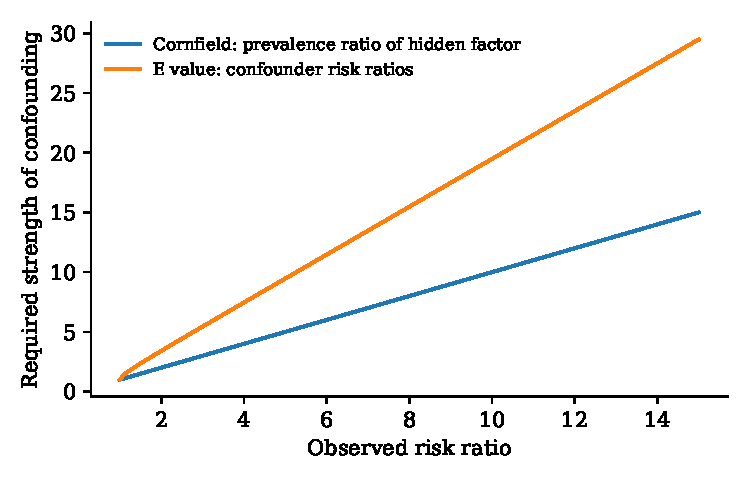
\includegraphics[width=\linewidth]{cornfield.pdf}
\caption{Strength of confounding needed to explain away an observed risk ratio: Cornfield's prevalence ratio and the E value, for observed risk ratios from 1 to 15; Cornfield's bound equals the observed risk ratio.}
\label{fig:cornfield}
\end{figure}

\subsection{The Bayesian form}

Take an unmeasured binary confounder $U$\index{sensitivity analysis!Bayesian form|textbf} with prevalence $\Prob(U = 1 \mid X, T) = \expit(a_0 + a_1 T + \ldots)$ and outcome model $\Prob(Y = 1 \mid T, U, X) = \expit(b_0 + \tau T + b_U U + \ldots)$. Data on $(X, T, Y)$ identify none of $a_0$, $a_1$ and $b_U$. Fixing $a_1$ and $b_U$ still leaves $\tau$ dependent on prevalence, so place informed priors on all three.

Given $(a_0, a_1, b_U)$, the identified part of the posterior for $\tau$ concentrates as $n$ grows; the unidentified part retains their prior conditional on the identified parameters, equal to their marginal prior only under a priori independence. McCandless, Gustafson and Levy (2007) integrate out these bias parameters and report the effect's marginal posterior; since the data barely update them, the prior carries real weight, and the virtue of the approach is that the weight is visible. Gustafson (2015) shows the limiting posterior is a mixture, over this conditional prior at the limit of the identified parameters, of point masses at the value of $\tau$ each implies (Proposition~\ref{prop:partial} and Appendix~\ref{app:theory}).

The Bayesian sensitivity analysis reports the posterior probability of a positive effect, given our beliefs about possible confounders. Cornfield's threshold becomes a statement about the prior: in the limit, the posterior probability of no positive effect is the prior probability, given the identified parameters at their limit, that $(a_0, a_1, b_U)$ lie where confounding explains the whole observed effect.

\subsection{Calibrating the prior}

The objection is that the prior is arbitrary. Three practices answer it\index{sensitivity analysis!calibrating the prior|textbf}.

\paragraph{Benchmarking against measured covariates.} The strongest measured confounder gives a reference point: scale priors on $(a_1, b_U)$ by its observed strengths.

\paragraph{Substantive knowledge.} Fisher's hypothesis named a specific candidate, a genetic factor. Twin studies, which Fisher himself cited, constrain how strongly genes could drive smoking; a prior on $a_1$ informed by them is not arbitrary.

\paragraph{Reporting a family.} Report the posterior under several priors, from optimistic to sceptical. Cornfield did this informally, showing that only an implausibly strong confounder could explain the data; a family of Bayesian analyses makes the argument quantitatively.

\paragraph{Lanarkshire revisited.} In the Lanarkshire milk experiment (Chapter~\ref{ch:mccullagh}), the hidden confounder is the teachers' judgement of poverty beyond recorded height and weight. Let $\hat\tau$ be the milk effect adjusted for initial size. Only the part of judged poverty unexplained by size can bias it, through its links to assignment and growth. Size supplies the benchmark: priors on $b_U$ centred at a fraction of the size coefficient, and on $a_1$ informed by how far the teachers' substitutions followed size, give a posterior for the milk effect reflecting both the data and the teachers.

\subsection{A Bayesian sensitivity analysis in numbers}

Take a simple linear setting\index{sensitivity analysis!worked example|textbf}. An adjusted analysis estimates an effect $\hat\tau = 0.30$ with standard error $0.05$. An unmeasured confounder $U$ with unit variance shifts the estimate by $a\,b_U$, where $a$ is the coefficient of $T$ in a regression of $U$ on $T$ given measured covariates and $b_U$ is the effect of $U$ on the outcome. Both are linear coefficients, the counterparts of the logit coefficients $a_1$ and $b_U$ used earlier.

Give the adjusted effect $\tau_{\mathrm{adj}}$ the normal posterior centred at $\hat\tau$, place independent priors on the two bias parameters, and subtract the bias:
\[
\tau = \tau_{\mathrm{adj}} - a\,b_U, \qquad \tau_{\mathrm{adj}} \sim N(0.30, 0.05^2), \qquad a \sim N(0, s^2), \qquad b_U \sim N(0, s^2),
\]
all three independent. Figure~\ref{fig:sens} plots, for each prior scale $s$, the share of 200,000 Monte Carlo draws with $\tau > 0$.

\begin{figure}[ht]
\centering
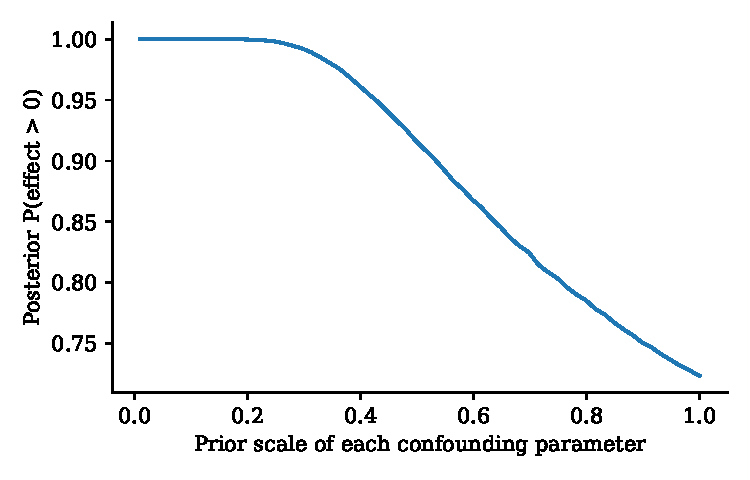
\includegraphics[width=\linewidth]{sensitivity.pdf}
\caption{Posterior probability that the effect is positive, for an estimate of 0.30 with standard error 0.05, as the prior scale of both confounding parameters increases.}
\label{fig:sens}
\end{figure}

Near $s = 0$ the posterior probability is essentially one: no confounding is believed possible, and the estimate is six standard errors from zero. At $s = 0.33$ it is 0.985, at $s = 0.66$ it falls to 0.84, and at $s = 1$, a prior standard deviation of one for both coefficients (a difference of one standard deviation of $U$ between the arms, one unit of outcome per standard deviation of $U$), it falls to 0.72.

The curve is the Bayesian analogue of an E value\index{E value}: it reports confidence in a positive effect under each prior scale. A reader who finds strong confounders implausible reads the left of the curve, a sceptic the right.

\paragraph{Lanarkshire in numbers.} The reanalysis sketched above for Lanarkshire can be run on the simulated trial of Section~\ref{sec:milk} in which the teachers went by an unrecorded nourishment score, with recorded size correlated 0.8 with it. In one such trial of 2,000 children the regression on treatment and size gives $\hat\tau = 0.35$ with standard error 0.025, and its interval, $[0.30, 0.40]$, misses the true 0.2.

Size supplies the benchmarks: the milk group is 0.71 standard deviations smaller, $a_S = -0.71$, and the gain falls by 0.53 per standard deviation of size, $b_S = -0.53$. The story fixes the signs, since the teachers favoured children who looked poorly and such children grow more, so the priors are centred away from zero, $a \sim N(k a_S, k^2 a_S^2)$ and $b_U \sim N(k b_S, k^2 b_S^2)$: a hidden score $k$ times as strong as size in its links to assignment and to growth. As for Figure~\ref{fig:sens}, the posterior of the effect comes from 200,000 Monte Carlo draws of $\hat\tau - a\,b_U$ plus an independent normal estimation error with standard deviation 0.025.
\begin{center}
\begin{tabular}{cccc}
\toprule
$k$ & Posterior mean & 95\% interval & $\Prob(\tau > 0)$ \\
\midrule
$1/4$ & $0.33$ & $[0.22, 0.41]$ & $> 0.999$ \\
$1/2$ & $0.26$ & $[-0.14, 0.52]$ & $0.93$ \\
$1$ & $-0.02$ & $[-1.62, 1.00]$ & $0.59$ \\
\bottomrule
\end{tabular}
\end{center}
With $k = 1/4$ the interval still misses the truth. In the simulation the hidden score is a little more than half as strong as size, $a = -0.39$ and $b_U = -0.3$, so the middle prior is the one centred near the truth; a real analysis does not know this, which is why it reports the family.

\subsection{Benchmarking with observed covariates in practice}

Cinelli and Hazlett (2020) proposed a widely used anchor for sensitivity parameters\index{sensitivity analysis!benchmarking with observed covariates|textbf}: express the strength of a hypothetical confounder as a multiple of the partial $R^2$ of an observed covariate with treatment and with outcome. A statement such as ``a confounder three times as strong as income would be needed to explain away the effect'' is then clear to anyone who knows how strong income is.

The Bayesian version sets the scale of the prior on the confounding parameters from the observed covariates' strengths. Take the 9,915 households of the 401(k) analysis of Chapter~\ref{ch:k401} (later in the book) and least squares fits on the nine covariates. The partial $R^2$ of a covariate with net financial assets is the share of the residual variance that adding it removes, given eligibility and the other eight covariates; with eligibility it is the same share given the other eight. In the 54 term basis of that chapter a covariate brings every term that involves it.
\begin{center}
\begin{tabular}{llcc}
\toprule
Covariate & Related to & Linear & 54 term basis \\
\midrule
Income & assets & $0.088$ & $0.167$ \\
Individual retirement account & assets & $0.039$ & $0.048$ \\
Income & eligibility & $0.029$ & $0.043$ \\
Defined benefit pension & eligibility & $0.044$ & $0.046$ \\
\bottomrule
\end{tabular}
\end{center}
Income is the observed covariate most strongly related to assets and one of the two most strongly related to eligibility; in the linear fits none of the remaining seven reaches 0.006 with eligibility. An unmeasured taste for saving might be as strongly related to assets as income is, but less to eligibility, which employers determine. A prior encoding that judgement gives a posterior combining the data with an explicit, checkable view of what is missing.

Cinelli and Hazlett (2020) also give the exact link between partial $R^2$ and bias in least squares. Let $\hat\tau$ be the treatment coefficient in the regression of the outcome on treatment and the measured covariates, with conventional least squares standard error $\mathrm{se}(\hat\tau)$ (a robust standard error breaks the identity) and $\mathrm{df}$ residual degrees of freedom. Adding a scalar confounder $U$ to that regression would move the coefficient, in absolute value, by
\[
\mathrm{se}(\hat\tau)\sqrt{\mathrm{df}\,\frac{R^2_{Y\sim U\mid T,X}\,R^2_{T\sim U\mid X}}{1 - R^2_{T\sim U\mid X}}},
\]
where $R^2_{Y\sim U\mid T,X}$ is the partial $R^2$ of $U$ with the outcome given treatment and covariates and $R^2_{T\sim U\mid X}$ its partial $R^2$ with treatment given covariates. A prior on these two partial $R^2$ values and on the direction of the shift, scaled by benchmarks like those for income, is therefore a prior on the bias.

In the linear setting of Figure~\ref{fig:sens}, the bias is $a\,b_U$. Income supplies the analogous coefficients $(a_{\mathrm{inc}}, b_{\mathrm{inc}})$: the coefficient of treatment in a regression of income on treatment, and income's coefficient in the outcome model. A zero centred prior on $(a, b_U)$ with scales a stated multiple of these benchmarks says the missing confounder is typically no stronger than that multiple of income; a firm upper limit needs bounded support. The scale then has a meaning: $s = 1$ can represent a confounder as strong as the strongest measured covariate.

Both the benchmark and hidden confounder strengths must be conditional on the other covariates. The strongest observed confounder was measured because someone thought of it, weak evidence that what remains is weaker. The prior should allow stronger hidden confounders.

\subsection{Sensitivity and partial identification}

Sensitivity analysis and partial identification\index{partial identification|textbf}\index{identification!partial|textbf} are two views of one situation. Partial identification reports the effects consistent with the data under weak assumptions (Manski 2003; the Tian and Pearl bounds above). Sensitivity analysis shows how the estimate moves with a sensitivity parameter. A Bayesian puts a prior on that parameter; the limiting posterior is the prior pushed through the identified set (Proposition~\ref{prop:partial}).

Manski's bounds\index{Manski bounds@Manski's bounds|textbf} without assumptions on selection are wide: for a binary outcome and treatment, the average effect lies in an interval of length one whatever the data. Monotone treatment response, monotone treatment selection and other shape restrictions narrow the bounds. Each corresponds to a restriction on the support of the prior, and a soft version, a prior putting most but not all mass on the restricted region, is often more honest than the hard restriction or none.

\section{In practice}

\paragraph{The target.} The targets are $\PN$, $\PS$ and $\PNS$. With observational data added, the position $u$ is not enough: two joint laws can share every margin and the value of $\PNS$ and still differ in $\PN$, as 0.68 and 0.99 do for the numbers of Section~\ref{sec:court}. Each posterior draw is then the eight cell probabilities $q_{xab} = \Prob\{X = x, Y(1) = a, Y(0) = b\}$, and
\[
\PN = \frac{q_{110}}{q_{110} + q_{111}}, \qquad \PS = \frac{q_{010}}{q_{000} + q_{010}}, \qquad \PNS = q_{010} + q_{110}.
\]
For the effect $\tau$ under unmeasured confounding, draw the identified parameters from their posterior and the sensitivity parameters from their prior conditional on them, then compute $\tau$. The conditional prior equals the marginal prior under a priori independence (Proposition~\ref{prop:partial}). The share of draws with $\tau > 0$ is the Bayesian answer to Cornfield's question.

\paragraph{What the analyst does differently.} State which probability of causation is sought, compute its bounds within covariate strata, and report the posterior under a stated prior and at least one alternative. With the experiment alone, put the prior on $u$; with both sources, on the eight cell law. For $u$, Figure~\ref{fig:pns} uses uniform and $\mathrm{Beta}(1/2, 1/2)$ priors, and a point mass at $u = 0$ states monotonicity.

Check agreement of observational and experimental margins beyond sampling error. For the same population, disagreement refutes exogeneity, so $1 - 1/\mathrm{RR}$ is not the number to report; agreement does not prove exogeneity. For different populations, the theorem's bounds do not apply.

For sensitivity analysis, report the Cornfield or E value threshold, then put priors on the confounding parameters calibrated against measured covariates and candidate confounders. Report $\Prob(\tau > 0)$ under priors from optimistic to sceptical, as in Figure~\ref{fig:sens}.

\paragraph{Against DML.} $\PN$, $\PS$ and $\PNS$ are not identified, so DML has no point to estimate. It can estimate their bounds, which are identified functionals. Kallus (2022) gives cross fitted, doubly robust estimators and confidence intervals for sharp bounds on the share a treatment harms, a quantity like $\PNS$, averaging bounds over covariate strata. The frequentist answer is an interval for each bound or a confidence set for the parameter. These bounds need no Bayesian machinery: reporting $\PN$ between 0.61 and 1 and leaving the decision to the court is honest work. When a verdict or a targeting rule with different values for conversion and deterrence requires a single number, a Bayesian combines the bounds with a prior and shows how much of the answer comes from it.

For the sensitivity target, DML estimates the identified adjusted effect. Frequentist sensitivity tools include Cornfield's inequality, Rosenbaum's $\Gamma$, the E value and Cinelli and Hazlett's partial $R^2$ benchmarks. Chernozhukov, Cinelli, Newey, Sharma and Syrgkanis (2022a) extend those benchmarks to DML: bias is bounded by an identified scale times two factors measuring the confounder's additions to the outcome regression and to the Riesz representer (inverse propensity weights for a binary treatment). A reader able to judge these thresholds needs no prior. The Bayesian bias model gives a probability and shows how much of it comes from the confounding priors, which the data barely update. It adds nothing to the estimate of the adjusted effect, and it cannot say which prior is right; the probability is only as good as the stated beliefs about the confounder.

\section*{Notes}

Pearl (2009, Chapter 9) treats the probabilities of causation; see Balke and Pearl (1997) for the noncompliance bounds themselves. The $\mathrm{Beta}(1/2, 1/2)$ prior on the position inside the bounds is the horseshoe shrinkage coefficient law of Carvalho, Polson and Scott (2010).

Sensitivity analysis begins with Cornfield and coauthors (1959), whose inequality answered Fisher's constitutional hypothesis on smoking (Chapter~\ref{ch:smoking}). For partial identification see Manski (1990, 2003), Gustafson (2015) and Moon and Schorfheide (2012). Conley, Hansen and Rossi (2012) apply the same logic to an instrument's exclusion restriction (Chapter~\ref{ch:iv}).

\begin{exercises}
\item\label{ex:ch11:1} Assuming that $X$ is independent of $(Y(0), Y(1))$, derive the experimental bounds on $\PN$ and $\PS$, analogous to those on $\PNS$.
\item\label{ex:ch11:2} Show that under exogeneity, $\Prob(y_x) = \Prob(y \mid x)$ and $\Prob(y_{x'}) = \Prob(y \mid x')$, the lower bound on $\PN$ equals $\max\{0, 1 - 1/\mathrm{RR}\}$ with $\mathrm{RR} = \Prob(y \mid x)/\Prob(y \mid x')$, which is $1 - 1/\mathrm{RR}$ when $\mathrm{RR} \geq 1$.
\item\label{ex:ch11:3} Set up the linear program whose solution gives the combined bounds on $\PNS$, and solve it for the hypothetical numbers of Figure~\ref{fig:pns} with observational rates of your choosing.
\item\label{ex:ch11:4} Under the Gaussian copula of Section~\ref{sec:ot} applied to latent normal variables underlying $Y(0)$ and $Y(1)$, compute $\PNS$ as a function of $\rho$ and the margins.
\item\label{ex:ch11:5} A plaintiff smoked and developed lung cancer, and the relevant risk ratio is 10. Compute the lower bound on $\PN$ under exogeneity and discuss what further assumptions would be needed to reach $\PN$ near one.
\item\label{ex:ch11:6} For the targeting problem with gain $g$ for a conversion, loss $L$ for a customer put off and incentive cost $c$, show that the risk difference alone decides when $g = L$, then derive the Bayes rule under a uniform prior on $u$ when $g \neq L$ and compare it with the minimax rule.

\item\label{ex:ch12:1} Show that, for fixed $f_1 > f_0$, the observed risk ratio in Cornfield's setup increases in $R = r_1/r_0$ and tends to $f_1/f_0$ as $R \to \infty$.
\item\label{ex:ch12:2} Derive the E value formula from the bounding factor $\mathrm{RR}_{EU}\mathrm{RR}_{UD}/(\mathrm{RR}_{EU} + \mathrm{RR}_{UD} - 1)$.
\item\label{ex:ch12:3} Compute the E value for risk ratios of 2, 9 and 20 and interpret each for the smoking literature.
\item\label{ex:ch12:4} Show that the limiting posterior in Proposition~\ref{prop:partial} is a point mass if and only if $h(\phi_0, \xi)$ is constant for almost every $\xi$ under the prior, and that when $h(\phi_0, \cdot)$ is continuous this is the same as being constant on the support of the prior on $\xi$.
\item\label{ex:ch12:5} For a Bayesian sensitivity analysis in the linear setting of Figure~\ref{fig:sens}, with $a \sim N(0, s_a^2)$ and $b_U \sim N(0, s_b^2)$, write the limiting posterior probability that $\tau > 0$ as a one-dimensional integral and show that it depends on the priors only through $\tau_0/(s_a s_b)$, where $\tau_0$ is the limit of the adjusted estimate.
\item\label{ex:ch12:6} Design a benchmarking prior for the milk experiment using the observed coefficient of initial size.
\end{exercises}

\chapter{Smoking and Lung Cancer}\label{ch:smoking}

\begin{tcolorbox}[colback=gray!6,colframe=gray!50,title=In brief,fonttitle=\normalfont\itshape,coltitle=black,colbacktitle=gray!15,boxrule=0.4pt,arc=1pt]
Fisher was right that observation cannot exclude every common cause and wrong about which way the evidence pointed. Cornfield's inequality, dose response, cessation and Mendelian randomization each constrain the alternatives, and a Bayesian synthesis would combine them with the assumptions in view.
\end{tcolorbox}

The smoking controversy\index{smoking and lung cancer|textbf} is the best known causal argument in the history of statistics. It pitted Fisher, the founder of modern experimental design, against observational evidence that proved right. It produced the first sensitivity analysis\index{sensitivity analysis}, an influential set of criteria for observational causation, and, later, the canonical example of Pearl's front door\index{front door criterion} criterion. 

\section{The evidence}

In 1950 Wynder and Graham in the United States and Doll and Hill in London published case control studies\index{case control study|textbf} comparing lung cancer patients with other hospital patients. Both found lung cancer patients far more likely to be heavy smokers\index{smoking and lung cancer!the evidence|textbf}.

Case control studies are open to bias in the choice of controls, in recall of past smoking, and in who reaches hospital, so Doll and Hill began a prospective study. In 1951 they wrote to the doctors of Britain, recorded their smoking habits, and followed their deaths. The British doctors study\index{British doctors study|textbf} reported first results in 1954 and ran for fifty years. Hammond and Horn (1958) ran a larger American cohort for the American Cancer Society. Both found a strong dose response: the more cigarettes smoked, the higher the lung cancer death rate, and risk fell among those who stopped.

A case control study starts from the outcome and looks back at exposure. It is efficient for a rare disease, since lung cancer patients are collected rather than waited for, but controls must come from the population that produced the cases, and recall must not depend on diagnosis. A cohort study records exposure and waits for the outcome. Recall cannot be coloured by diagnosis, though habits can still be misreported, and comparison within the cohort removes the choice of controls. Neither design assigns smoking: the doctors' smokers and nonsmokers were self selected groups, which was Fisher's opening.

Case control and cohort studies estimate the same risk ratio under different sampling designs and biases. The case control odds ratio approximates it because lung cancer is rare\index{rare disease assumption|textbf}. A combined model needs a bias term for each design. The dose response and the fall in risk after quitting are not further estimates of that number; they are features of the data that any alternative explanation must reproduce.

\section{Fisher's objection}

Fisher entered the debate\index{Fisher, Ronald A.!objection to the smoking evidence|textbf} in 1957. He made three arguments\index{smoking and lung cancer!Fisher's objection|textbf}.

First, an observational association can always be explained by a common cause. Fisher proposed a constitutional hypothesis\index{constitutional hypothesis|textbf}: a genetic disposition that inclined people both to smoke and to develop lung cancer.

Second, using data on twins, he showed that identical twins were more alike in their smoking habits than fraternal twins, as a genetic hypothesis would predict.

Third, he pointed to anomalies, including the finding in Doll and Hill's case control study that inhalers did not show the expected higher risk.

Fisher consulted for the Tobacco Manufacturers' Standing Committee from 1956 (Stolley 1991). We do not think it explains his position. Randomization was the deepest commitment of his scientific life, and here randomization was impossible. He saw correctly that observation alone could not exclude every common cause, but he was wrong about which way the evidence pointed.

\section{Cornfield's answer}

Cornfield\index{Cornfield inequality@Cornfield's inequality}'s 1959 review, discussed in Section~\ref{sec:sensitivity}, turned Fisher's possibility into a quantitative requirement. If smokers had nine times the lung cancer risk of nonsmokers, a constitutional factor, coded so that $U = 1$ raises the risk of lung cancer, would need to be at least nine times as common among smokers. For heavy smokers, those smoking more than two packs a day, with a risk ratio against nonsmokers of about 60, it would need to be some sixty times as common.

Three further facts told against the constitutional hypothesis. A binary genotype could produce the steep dose response only by being far more common among the heaviest smokers than among nonsmokers, and a fixed genotype could explain the fall in risk after quitting only if it were also associated with who quits, and when. And lung cancer rates had risen sharply over a few decades, tracking cigarette consumption with a lag, far too fast for any genetic change in a population.

The 1964 report of the United States Surgeon General's committee\index{Surgeon General report|textbf} concluded that cigarette smoking is causally related to lung cancer in men. 

\section{The twin studies}

Fisher's second argument rested on twins\index{twin study|textbf}\index{twins}. Concordance in smoking bears on one side of Cornfield's requirement, how much more common a genotype is among smokers than among nonsmokers. It says nothing about whether the same genotype raises the risk of lung cancer, so concordance alone cannot show that genes confound the link between smoking and cancer.

A direct test compares monozygotic twins discordant for smoking. Within a pair the genotype is fixed, so the constitutional hypothesis alone predicts no excess lung cancer in the smoking twin. Other common causes can still differ within pairs. Hjelmborg and coauthors (2017) made this comparison in four Nordic twin cohorts, 43,512 monozygotic and 71,895 same sex dizygotic twins whose smoking was recorded before any cancer diagnosis, followed for a median of 28.5 years. In pairs discordant for smoking, the hazard ratio for lung cancer of the twin who had ever smoked against the twin who never had was 5.4 (95\% interval 2.1 to 14.0) in monozygotic pairs and 5.0 (3.2 to 7.9) in dizygotic pairs. The smoking twins show the excess that the constitutional hypothesis forbids.

\section{The inhalation paradox}

Fisher made much of a puzzle\index{inhalation paradox|textbf} in Doll and Hill's case control data: smokers who reported inhaling showed no higher lung cancer risk than those who did not, although inhalers should be at greater risk if smoke causes cancer by reaching the lungs.

Reported inhalation is a crude measure, and smokers may not know whether they inhale deeply. Inhalers may smoke cigarettes down to shorter butts or choose different tobacco. And deeply inhaled smoke may deposit carcinogens in different parts of the respiratory tract.

Substantial measurement error can hide an association even when the underlying quantity is causally important. Fisher read absence of association as evidence of absence. What the null excludes depends on misclassification rates and whether they differ between cases and controls. A Bayesian measurement error\index{measurement error} model, with validation data or stated priors on those rates, would show how wide a range of inhalation effects the data allow.

\section{The front door}
\begin{figure}[ht]
\centering
\begin{tikzpicture}[node distance=16mm]
\node[v] (S) {$S$};
\node[v,right=of S] (M) {$M$};
\node[v,right=of M] (C) {$C$};
\node[h,above=10mm of M] (U) {$U$};
\draw[e] (S) -- (M); \draw[e] (M) -- (C); \draw[e] (U) -- (S); \draw[e] (U) -- (C);
\end{tikzpicture}
\caption{The front door graph: smoking $S$ affects cancer $C$ only through tar $M$, and a hidden genotype $U$, dashed, affects smoking and cancer but not tar.}
\label{fig:dagfd}
\end{figure}


Pearl illustrated front door identification\index{front door criterion|textbf} with smoking\index{front door criterion!application to smoking|textbf} (Pearl 2009; Pearl and Mackenzie 2018). Suppose smoking $S$ causes lung cancer $C$ only through tar deposits $M$ in the lungs, and a hidden genotype $U$ affects both $S$ and $C$ but not $M$ directly (Figure~\ref{fig:dagfd}). If also every pair of values $(s, m)$ has positive probability, the effect of $S$ on $C$ is identified although $U$ is unmeasured\index{front door criterion!formula|textbf}:
\begin{equation}
\Prob(c \mid do(s)) = \sum_m \Prob(m \mid s) \sum_{s'} \Prob(c \mid m, s')\Prob(s').
\label{eq:frontdoor}
\end{equation}
The inner sum is the effect of tar on cancer, adjusted for smoking, which blocks the back door path from tar through the genotype to cancer. The outer sum chains it with the effect of smoking on tar, unconfounded because the genotype does not affect tar directly.

A worked example shows how the formula removes the genotype. The numbers are illustrative. Let $\Prob(S=1)=0.5$, $\Prob(M=1\mid S=1)=0.9$ and $\Prob(M=1\mid S=0)=0.1$, and let the cancer rates $\Prob(C=1\mid m,s)$ be $0.15, 0.10, 0.10, 0.05$ for $(m,s)=(1,1),(1,0),(0,1),(0,0)$. The observational contrast is $\Prob(C=1\mid S=1)-\Prob(C=1\mid S=0)=0.145-0.055=0.09$. The inner sums in \eqref{eq:frontdoor} are $0.5\cdot0.15+0.5\cdot0.10=0.125$ for $m=1$ and $0.5\cdot0.10+0.5\cdot0.05=0.075$ for $m=0$, so
\begin{align*}
\Prob(C=1\mid do(S=1)) &= 0.9(0.125)+0.1(0.075)=0.12,\\
\Prob(C=1\mid do(S=0)) &= 0.1(0.125)+0.9(0.075)=0.08,
\end{align*}
a causal risk difference of $0.04$. More than half of the observational contrast, $0.05$ of the $0.09$, is confounding by the genotype.

We simulated this structure with 20,000 people and binary variables: the genotype is present in 30\%, $\Prob(S = 1 \mid U) = \expit(-0.5 + 2U)$, $\Prob(M = 1 \mid S) = \expit(-2 + 4S)$ and $\Prob(C = 1 \mid M, U) = \expit(-3 + 1.5M + 1.5U)$, so about half the population smokes and a fifth develops cancer. The true effect, the risk difference $\Prob(C = 1 \mid do(S = 1)) - \Prob(C = 1 \mid do(S = 0))$, is 0.145. Over 100 replications the naive contrast between smokers and nonsmokers averaged 0.227, inflated by the genotype. The front door formula \eqref{eq:frontdoor} gave 0.145. Figure~\ref{fig:frontdoor} shows the errors.

\begin{figure}[ht]
\centering
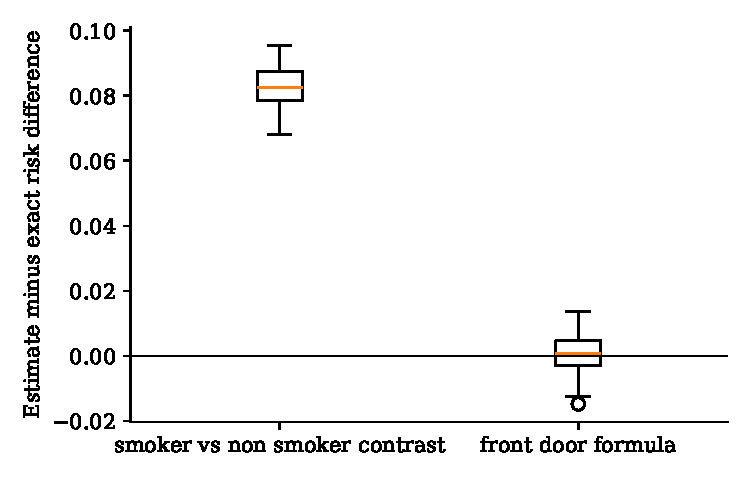
\includegraphics[width=\linewidth]{frontdoor.pdf}
\caption{Estimate minus the exact population risk difference, 0.145, for the smoker versus nonsmoker contrast and for the front door formula, boxplots over 100 replications of 20,000 people in a simulated population with a hidden genotype.}
\label{fig:frontdoor}
\end{figure}

The front door estimates above plug sample proportions into \eqref{eq:frontdoor}. A Bayesian version gives independent uniform, $\mathrm{Beta}(1,1)$, priors to the seven probabilities of the binary model: $\Prob(S=1)$, the two values of $\Prob(M=1\mid S=s)$ and the four values of $\Prob(C=1\mid M=m,S=s)$. Each posterior is a Beta updated with its own counts of successes and failures, and each joint posterior draw, pushed through the formula at $s=1$ and at $s=0$, gives a draw of the risk difference. This is the accounting thesis of the book in miniature: the effect is a functional of the model, so a posterior for the model is a posterior for the effect. In one simulated data set of 20,000 people the posterior mean of the risk difference is 0.153 and the 95\% interval runs from 0.140 to 0.165, which covers the truth 0.1445; across 500 further data sets such intervals covered it 95\% of the time. The naive contrast, 0.233 with interval 0.222 to 0.243, misses it.

The front door assumptions are strong: tar must carry the whole effect of smoking, the genotype must not affect tar, and nothing but smoking may confound tar and cancer. The first two are not literally true: smoking affects cancer through many pathways, and genes affect how tar is cleared. But identification can come from structure as well as adjustment, and in a Bayesian analysis structural assumptions are part of the model, to be relaxed with priors when doubted.

\section{A model first analysis}

Here is how a Bayesian would approach the question today\index{smoking and lung cancer!model first analysis|textbf} with cohort data like the British doctors study\index{British doctors study}.

\paragraph{The model.} Model the hazard of lung cancer death as a function of age, cumulative smoking, time since quitting and other covariates, with flexible terms for the dose response and horseshoe priors on interactions. 

\paragraph{The accounting.} The effect of smoking is any of several functionals: the difference in lifetime risk between a lifelong smoker and a never smoker of the same birth cohort; the risk reduction from quitting at age 40; the population attributable fraction\index{population attributable fraction|textbf}, the share of lung cancer deaths avoided if no one smoked. Each is a functional of the fitted model under a chosen covariate law $Q$; the attributable fraction also needs the share of smokers at each covariate value. Smokers also die earlier of other causes, so a lifetime risk of lung cancer death is a cumulative incidence (Andersen et al. 2012). For a given covariate profile and smoking history, let $\lambda_C(t)$ and $\lambda_O(t)$ be the hazards of lung cancer death and of death from other causes under that history. The risk of lung cancer death by time $t$ is
\[
F_C(t)=\int_0^t \lambda_C(v)\exp\left[-\int_0^v\{\lambda_C(u)+\lambda_O(u)\}\,du\right]dv,
\]
so the lifetime risk needs a model for death from other causes as well as for lung cancer.

\paragraph{The confounding.} Fisher's genotype enters as an unmeasured binary $U$ with a prior on its prevalence ratio between smokers and nonsmokers and on its effect on cancer. Twin studies of smoking concordance inform the first. 

\paragraph{The attribution.} For an individual smoker with lung cancer, $\PN$ is bounded below by $1 - 1/\mathrm{RR}$ under exogeneity (Chapter~\ref{ch:tianpearl}). With a risk ratio\index{risk ratio} of 9, that is about 0.89. Figure~\ref{fig:pnbound} plots the bound against the risk ratio: it passes one half, the civil standard of more probable than not, at a risk ratio of 2, and for heavy smokers, with a risk ratio near 60, it is 0.98. The bound applies to a smoker drawn at random from the lung cancer cases of the group whose risk ratio it uses. For a plaintiff with known dose or other characteristics, use the matching group's risk ratio and exogeneity assumption; the population ratio can put her bound too high or too low (Exercise~\ref{ex:ch13:6}).

\begin{figure}[ht]
\centering
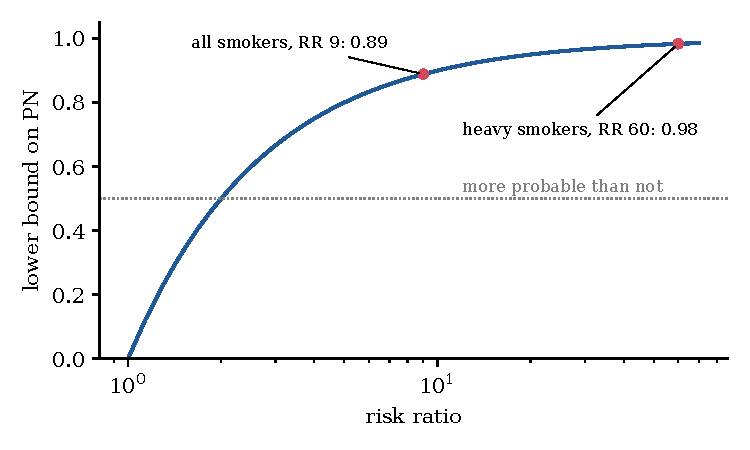
\includegraphics[width=0.85\linewidth]{pn_bound.pdf}
\caption{The lower bound $1 - 1/\mathrm{RR}$ on the probability of necessity under exogeneity, against the risk ratio on a log scale.}
\label{fig:pnbound}
\end{figure}

Without exogeneity, the Tian and Pearl bounds widen, and the Bayesian posterior for $\PN$ depends on the prior for $U$.



\paragraph{A modern Bayesian synthesis.} A Bayesian synthesis would combine in one model cohort dose responses and quitting effects, case control risk ratios through the odds ratios, a prior on genetic confounding informed by twins, and Mendelian randomization evidence on smoking heaviness. Each source would have its own likelihood, bias model and assumptions. The conclusion, which no serious analyst doubts, would not change; the synthesis would show how it depends on each source and assumption.

\paragraph{A computed illustration.} The numbers below come from stated priors, and no cohort data enter. Let $U$ be carried by a fraction $f_1$ of smokers and $f_0 = f_1/\mathrm{PR}$ of nonsmokers, let it multiply the risk of lung cancer by $R$ in both groups, and suppose smoking is unconfounded within levels of $U$. If $r_{s0}$ is the risk at smoking status $s$ when $U=0$, the observed risk in group $s$ is $r_{s0}\{1+f_s(R-1)\}$, so
\[
\mathrm{RR}=\frac{r_{10}}{r_{00}}\,B,\qquad B=\frac{1+f_1(R-1)}{1+f_0(R-1)},\qquad \tau=\log\frac{r_{10}}{r_{00}}=\log\frac{\mathrm{RR}}{B}.
\]
Here $B$ is the factor in Cornfield's proof and $\tau$ is the log risk ratio of smoking within levels of $U$. With the observed risk ratio RR fixed at 9 or 60, as a large cohort would fix it, and with $(f_1, \mathrm{PR}, R)$ a priori independent of the observed risks, the posterior of $\tau$ is the prior on $(f_1, \mathrm{PR}, R)$ pushed through $B$ (Proposition~\ref{prop:partial}), restricted to values that keep every stratum risk between zero and one. At the nonsmoker risk 0.0002 of Table~\ref{tab:smokingbayes} the restriction removes at most $1.4 \times 10^{-4}$ of the prior mass. Under a continuous prior the event $\tau = 0$ has probability zero, so we report the probability of no positive effect, $\Prob(\tau\leq 0)=\Prob(B\geq\mathrm{RR})$, the prior mass of Cornfield's region. Because $B\leq\min(\mathrm{PR},R)$, that region needs both PR and $R$ to be at least as large as RR.

Both priors make $f_1$ uniform and $\log \mathrm{PR}$ and $\log R$ independent and half normal. The sceptical prior gives PR and $R$ each a median of 3.8 and a 95th percentile of 50. The twin informed prior keeps that for $R$ and gives PR a median of 1.6 and a 95th percentile of 4. The 4 is illustrative, not elicited.

\begin{table}[ht]
\centering
\caption{Limiting posterior of the bias model of Section~\ref{sec:sensitivity} under two illustrative priors for the genotype. $L$ is the Tian and Pearl lower bound on $\PN$ without exogeneity, and $\PN$ has its position within the bounds uniform. The probability of no positive effect comes from numerical integration and the other summaries from 4,000,000 prior draws, both restricted to values whose stratum risks lie between zero and one, with a cohort of smoking prevalence 0.5 and nonsmoker risk 0.0002.}
\label{tab:smokingbayes}
\small
\begin{tabular}{@{}lcccc@{}}
\toprule
Prior & \shortstack{$\Prob$(no positive\\effect)} & $\Prob(L > 1/2)$ & \shortstack{$\PN$\\mean} & \shortstack{$\PN$ 95\%\\interval} \\
\midrule
\multicolumn{5}{@{}l}{Observed risk ratio 9, E value 17.5} \\
Sceptical & 0.022 & 0.923 & 0.886 & [0.512, 0.996] \\
Twin informed & $4.4 \times 10^{-5}$ & 0.998 & 0.925 & [0.802, 0.997] \\
\midrule
\multicolumn{5}{@{}l}{Observed risk ratio 60, E value 119.5} \\
Sceptical & $2.5 \times 10^{-4}$ & 0.999 & 0.982 & [0.922, 0.999] \\
Twin informed & $< 10^{-6}$ & 1.000 & 0.989 & [0.970, 0.999] \\
\bottomrule
\end{tabular}
\end{table}


At a risk ratio of 9 (Table~\ref{tab:smokingbayes}) the probability of no positive effect is 0.022 under the sceptical prior and $4.4 \times 10^{-5}$ under the twin informed one, and it is 0.0023 if the twin informed 95th percentile for PR is 9 instead of 4. At 60 the probabilities are $2.5 \times 10^{-4}$ and below $10^{-6}$. Without exogeneity the Tian and Pearl lower bound on $\PN$ follows from the cell probabilities each draw implies, and in this model it reduces to $L=\max\{0,\,1-B/\mathrm{RR}\}=\max\{0,\,1-e^{-\tau}\}$, the exogeneity bound $1-1/\mathrm{RR}$ with the risk ratio within levels of $U$ in place of the observed one. The upper bound can fall below one, but it equals one on every draw we checked, about 4,000,000 for each prior and risk ratio, at smoker shares from 0.2 to 0.8 and nonsmoker risks from $10^{-4}$ to $10^{-3}$. The table gives $\PN$ a uniform position between the bounds, independently of each parameter draw, so its summaries depend on both this prior and the prior for $U$. At a risk ratio of 9 under the sceptical prior $L$ has posterior mean 0.77, against 0.89 under exogeneity, and exceeds one half with probability 0.92.

\section{Bradford Hill's considerations as prior information}

Bradford Hill\index{Hill, Austin Bradford|see{Bradford Hill's considerations}}'s 1965 lecture listed nine considerations\index{Bradford Hill considerations@Bradford Hill's considerations|textbf} for judging whether an association is causal. He insisted they were not a checklist and that none was necessary or sufficient. A Bayesian can say what each contributes.

\paragraph{Strength.} A large risk ratio requires a strong confounder to explain it, Cornfield's point. Under any fixed prior on confounding strength, a larger risk ratio pushes the posterior probability of a real effect toward one.

\paragraph{Consistency.} Agreement across populations, designs and investigators makes a single source of bias less likely. In a hierarchical model across studies, consistency shows up as small between study variance and a posterior for the common effect that is robust to dropping any one study.

\paragraph{Specificity.} An exposure that causes one disease rather than many is easier to believe. Smoking, which causes many diseases, seemed to violate it, though Hill (1965) saw specificity in the size of the lung cancer association, and he rightly gave the criterion little weight.

\paragraph{Temporality.} The cause must precede the effect. We take this as logically necessary, whatever Hill's warning: a model constraint rather than evidence within it.

\paragraph{Biological gradient.} Suppose a binary $U$ explains the whole dose response\index{dose response}, smoking itself having no effect, and let $f_d$ be its prevalence among smokers at dose $d$ and $f_0$ its prevalence among nonsmokers. Cornfield's inequality holds at every dose level, so $f_d/f_0\geq\mathrm{RR}(d)$ at every $d$. Since $f_d\leq 1$, a risk ratio near 60 for the heaviest smokers gives $f_0\leq 1/60$: at most one nonsmoker in sixty could carry $U$. Smoothness adds little on its own, since a prevalence that rises smoothly with dose reproduces any smooth gradient; the constraint is the size of the ratios, and it tightens only if the model also limits how $f_d$ can vary with dose.

\paragraph{Plausibility and coherence.} Agreement with known biology is prior information: animal experiments showing that tobacco tar induces tumours raise the prior probability of a causal effect.

\paragraph{Experiment.} The fall in risk after quitting is the semi-experimental evidence Hill had in mind, and evidence against any time invariant confounder not associated with who quits (Exercise~\ref{ex:ch13:5}). Quitting data also give a second Cornfield condition: a genotype explaining the whole risk gap between continuing smokers and long-term quitters must have a prevalence ratio between those groups at least as large as their observed risk ratio.

\paragraph{Analogy.} Similar exposures with known effects make an effect more plausible; this too is prior information.

\section{Mendelian randomization}

Chapter~\ref{ch:iv} introduced Mendelian randomization\index{Mendelian randomization}. For smoking, variants in the nicotinic acetylcholine receptor cluster on chromosome 15 are associated with cigarettes smoked per day among smokers (Thorgeirsson et al. 2008; Tobacco and Genetics Consortium 2010). Assigned at conception, these variants give variation in smoking heaviness unrelated to most of the social and behavioural confounders of smoking.

Fisher's constitutional hypothesis said that genes confound the association; Mendelian randomization uses genes as instruments for smoking. A gene causing both smoking and cancer by separate pathways, as Fisher supposed, would violate the exclusion restriction. Modern analyses use many variants and allow for pleiotropy. Larsson et al. (2020) combined more than 340 variants associated with starting to smoke, checked the main estimate against estimators that tolerate some invalid instruments, and found an odds ratio for lung cancer of 1.80 (95\% interval 1.59 to 2.03) per standard deviation of genetically predicted smoking initiation in the International Lung Cancer Consortium data, and 2.26 in UK Biobank.

A second check looks at never smokers: a variant affecting cancer only through smoking should have no effect there, and an association would favour Fisher's separate pathway. The check is not clean. If the variant also affects smoking initiation, restricting to never smokers selects on a collider, a common effect of the variant and other causes of smoking (Section~\ref{fw:sec:pearl}); if any of those causes also affects cancer, selection can create or hide an association (Gkatzionis and Burgess 2019).

Pooled analyses find no association between the chromosome 15 variants and lung cancer among never smokers. The International Lung Cancer Consortium found none, while white ever smokers there show an odds ratio of 1.26 per risk allele (Truong et al. 2010), and Wang et al. (2011) report an odds ratio of 1.09 (95\% interval 0.94 to 1.28) from 2,405 never smokers with lung cancer and 7,622 controls. That interval does not exclude an effect as large as the one in smokers, and an early genome wide report had found similar risks whatever the smoking status (Hung et al. 2008), so the check favours Fisher's critics without settling the question on its own.

\section{In practice}

\paragraph{The target.} Each posterior draw of the hazard model and confounding parameters gives the population attributable fraction and benefit of quitting\index{smoking and lung cancer!benefit of quitting|textbf} by averaging fitted risks over the appropriate population. For an individual's probability of necessity, compute the Tian and Pearl bounds from each draw and draw a position within them. The same draws give a lifelong smoker's lifetime risk.

\paragraph{What the analyst does differently.} Before fitting anything, write down the alternative explanation, as Fisher did, and ask what the data require of it; here the requirement is Cornfield's. Fit a risk model with a flexible dose response and a term for time since quitting, give the unmeasured confounder a prior calibrated to what is known, and report the posterior probability of no positive effect under that prior and under a sceptical one. For a plaintiff, report the bound $1 - 1/\mathrm{RR}$ for the group matching her dose and other known characteristics, say that it assumes exogeneity within that group, then give the posterior without that assumption. Fit a measurement error model for a crudely measured variable such as inhalation rather than reading a null association as evidence of no effect.

\paragraph{Against DML.} DML's guarantees for the cohort comparison assume all confounders are measured, precisely the point in dispute. Its instrumental variable score (Chapter~\ref{ch:iv}) replaces this with an exclusion restriction, which for a genetic instrument is the one Fisher's genotype would break. Either way the output is one number with an asymptotic interval, which by itself answers neither Fisher's objection nor the court's question. The sensitivity bounds that carry Cornfield's argument to DML (Section~\ref{sec:sensitivity}) quantify the confounding needed to overturn the estimate, meeting part of Fisher's objection, but give a threshold where the court asks for a probability. DML has no place for a prior on the genotype informed by the twin studies or for the dose response as evidence against an alternative, and it cannot combine cohort, case control, twin and Mendelian randomization evidence in one posterior. It is adequate for a single average effect with rich measured covariates and no serious unmeasured confounder, perhaps a comparison within a cohort adjusting for age and occupation. The full smoking question asks what the data say against a named alternative, and the Bayesian synthesis would answer it with the assumptions in view.

\section*{Notes}

The case control studies of 1950 are Wynder and Graham (1950) and Doll and Hill (1950), and the British doctors study first reported in Doll and Hill (1954). Fisher's letters and short book are Fisher (1957, 1958, 1959). Cornfield's inequality appears in Cornfield and coauthors (1959), the nine considerations in Hill (1965), and the Surgeon General's report is United States Department of Health, Education, and Welfare (1964).

For the front door see Pearl (1995, 2009) and Pearl and Mackenzie (2018); Appendix~\ref{app:graphs} derives the formula with the do calculus. Chapter~\ref{ch:tianpearl} develops Tian and Pearl's (2000) bounds and the sensitivity methods of VanderWeele and Ding (2017), Rosenbaum (2002), and McCandless, Gustafson and Levy (2007). The computed illustration integrates over bias parameters as McCandless, Gustafson and Levy do; Gustafson (2015) treats its partial identification setting. Chapter~\ref{ch:iv} gives the assumptions of Mendelian randomization (Katan 1986; Davey Smith and Ebrahim 2003).

The chapter reanalyses no historical data. The hazard model of the model first analysis, the measurement error model for inhalation and the twin cohorts are described and not fitted; what we compute is the front door simulation and the prior to posterior illustration of Cornfield's region.

\begin{exercises}
\item\label{ex:ch13:1} Derive the front door formula \eqref{eq:frontdoor} from the structural assumptions using the rules of the do calculus in Appendix~\ref{app:graphs}, justifying each step by the separation it needs in the graph.
\item\label{ex:ch13:2} In the simulation of Figure~\ref{fig:frontdoor}, add a direct effect of the genotype on tar and show how the front door estimate becomes biased.
\item\label{ex:ch13:3} Write the population attributable fraction as a functional of a fitted risk model, and explain why it depends on the law $Q_{SX}$ of smoking status and covariates in the population of interest, and not on the covariate law $Q$ alone.
\item\label{ex:ch13:4} Fisher's twin argument showed that smoking habits were more concordant in identical twins. Explain how such data could be used to set a prior on the genotype prevalence ratio in a Bayesian sensitivity analysis.
\item\label{ex:ch13:5} Among people who smoked before a common decision age, let $A$ indicate quitting at that age, $H$ the prior smoking and health history, and $Y$ lung cancer over a fixed follow up period with complete follow up. Suppose smoking has no effect on lung cancer, a fixed binary genotype $U$ raises the risk, and, given $U$ and $H$, quitting carries no further information about risk: $\Prob(Y=1\mid A,U,H)=r(U,H)$ with $r(1,h)>r(0,h)$. Show that, within a history stratum containing both quitters and continuing smokers, their risks can differ only if $U$ is associated with $A$ in that stratum, and give an example showing that the claim fails without the assumption on $r$. Construct an example in which $U$ has no effect on the decision to quit but is associated with it among smokers, because $U$ and some cause of quitting both lead people to start smoking. Then show that $U\indep A\mid H$ implies equal risks for quitters and continuing smokers within each history stratum, and say which implication of this can be tested without measuring $U$.
\item\label{ex:ch13:6} A cohort of smokers has dose specific risk ratios $\mathrm{RR}(d)$ against a common nonsmoker risk, and a share $w_d$ of the smokers is at dose $d$. Show that the average of the lower bounds $1 - 1/\mathrm{RR}(d)$ over the smokers who develop cancer equals $1 - 1/\mathrm{RR}$ for the single risk ratio $\mathrm{RR} = \sum_d w_d \mathrm{RR}(d)$, and say for which plaintiffs the dose specific bound exceeds the single ratio bound.
\end{exercises}

\part{Designs and Applications}
\chapter{Difference in Differences with the Horseshoe}\label{ch:did}

\begin{tcolorbox}[colback=gray!6,colframe=gray!50,title=In brief,fonttitle=\normalfont\itshape,coltitle=black,colbacktitle=gray!15,boxrule=0.4pt,arc=1pt]
Two way fixed effects is a weighted average of cohort by time effects with possibly negative weights. The horseshoe difference in differences estimator models those cells directly, with an unshrunk event time path, horseshoe cohort deviations and horseshoe departures from parallel trends, and reports every summary as an accounting of the posterior.
\end{tcolorbox}

Difference in differences\index{difference in differences|textbf} reads a policy's effect from the change in the gap between adopters and nonadopters from before to after. We introduce a horseshoe\index{horseshoe prior} estimator for heterogeneous effects under staggered adoption and departures from parallel trends.

\section{The model behind the design}

Unit $i$ in period $t$ has outcome $Y_{it}$ and adoption period\index{staggered adoption|textbf} $G_i$, with $G_i = \infty$ for units that never adopt. The canonical model for untreated outcomes is two way additive:
\begin{equation}
Y_{it}(\infty) = \alpha_i + \gamma_t + \varepsilon_{it}.
\label{eq:twoway}
\end{equation}
Parallel trends\index{parallel trends|textbf} says that \eqref{eq:twoway} holds for every unit, adopters included, with $\E(\varepsilon_{it}\mid G_i) = 0$ in every period, so that without the policy each adoption cohort's mean outcome would have moved in step with that of the never adopting units. Treated outcomes add an effect that may depend on adoption cohort\index{cohort|textbf} $g$ and time since adoption $e = t - g$:
\[
Y_{it}(g) = Y_{it}(\infty) + \tau_{g,e}, \qquad e \geq 0.
\]
The cohort by event time\index{event time|textbf} effects $\tau_{g,e}$ form a matrix, and every summary a study reports is a weighted sum of its cells. Parallel trends is a statement about a model for untreated outcomes, equation \eqref{eq:twoway}, and not about an estimator. Counts of treated unit periods give the average effect on the treated\index{effect on the treated}, the same counts within one event time give the event study\index{event study|textbf} path, and weights on one cohort give that cohort's experience. Each cohort appears only at the event times its adoption date allows, so some cells rest on very few observations and every summary must carry that uncertainty.

\section{What two way fixed effects estimates}

Two way fixed effects\index{two way fixed effects|textbf}\index{TWFE|see{two way fixed effects}} regresses $Y_{it}$ on unit and period dummies and $D_{it}$, equal to one from adoption on. Goodman Bacon (2021), de Chaisemartin and D'Haultf\oe uille (2020), and Sun and Abraham (2021) showed that, when effects vary across cohorts or over time, the coefficient on $D_{it}$ is a weighted average of the $\tau_{g,e}$ in which some weights can be negative\index{two way fixed effects!negative weights|textbf}\index{negative weights|see{two way fixed effects}}.

\begin{proposition}\label{prop:twfe}
Fix the adoption dates and observation pattern, denoted by $\mathcal G$, and suppose \eqref{eq:twoway} holds with $\E(\varepsilon_{it}\mid\mathcal G)=0$ and $Y_{it}=Y_{it}(\infty)+D_{it}\tau_{G_i,t-G_i}$. Let $\tilde D$ be treatment residualized on unit and period dummies, and assume $S=\sum_{it}\tilde D_{it}^2>0$. The conditional mean of the sample two way fixed effects\index{two way fixed effects} coefficient is
\[
\beta_{\mathrm{TWFE}}:=\E(\hat\beta_{\mathrm{TWFE}}\mid\mathcal G)=\sum_{(g,e)}\omega_{g,e}\tau_{g,e},\qquad
\omega_{g,e}=\frac{\sum_{\{(i,t):G_i=g,\ t-g=e\}}\tilde D_{it}}{S},
\]
where the sum is over observed treated cells and $\sum_{(g,e)}\omega_{g,e}=1$.
\end{proposition}

\begin{proof}
The Frisch Waugh Lovell theorem and $\sum_{it}\tilde D_{it}D_{it}=S$ give
\[
\hat\beta_{\mathrm{TWFE}}=\sum_{(g,e)}\omega_{g,e}\tau_{g,e}+\frac{\sum_{it}\tilde D_{it}\varepsilon_{it}}{S}.
\]
The fixed effects vanish by orthogonality. Conditional expectation given $\mathcal G$ removes the error term; the same identity gives $\sum_{(g,e)}\omega_{g,e}=1$.
\end{proof}

Early adopters' late observations have the smallest, possibly negative, residualized treatment because unit and period fixed effects absorb much of their treatment status. When effects grow with exposure, these cells have the largest effects and the smallest or negative weights, so two way fixed effects can understate the effect or reverse its sign. In the 500 simulated panels of 40 units of the design used below, the four latest cells of the period 4 cohort get weight $-0.026$ each on average, from $-0.062$ to $0.004$ across panels; the castle panel of the application has no negative weight at all, its smallest cell weight being 0.008 because 29 of the 50 states never adopt. Appendix~\ref{app:theory} gives the weights in a balanced panel.

\section{The horseshoe difference in differences estimator}

Untreated outcomes satisfy\index{difference in differences!horseshoe estimator|textbf}
\begin{equation}
Y_{it}(\infty) = \alpha_i + \gamma_t + \delta_i\,\tilde t + \varepsilon_{it}, \qquad \varepsilon_{it} \sim N(0, \sigma^2),
\label{eq:hsdid0}
\end{equation}
with $\tilde t$ standardized time and $\delta_i$ a unit specific departure from parallel trends\index{parallel trends!unit specific departures|textbf}. Effects decompose as
\begin{equation}
\tau_{g,e} = \theta_e + u_{g,e},
\label{eq:hsdid1}
\end{equation}
a common event time path $\theta_e$ plus cohort deviations $u_{g,e}$. Proposition~\ref{gr:prop:hstest} studies the same split, a common effect with horseshoe departures, as a test of whether the effect is stable across strata. Adopters may also lift or dip just before adoption, through anticipation or for reasons the unit trends do not absorb, so the observed outcome is
\begin{equation}
Y_{it} = Y_{it}(\infty) + \sum_{k=2}^{5}\ell_k\,\mathbf 1\{t - G_i = -k\} + D_{it}\,\tau_{G_i,\,t - G_i},
\label{eq:hsdid2}
\end{equation}
where the lead coefficients\index{lead coefficient|textbf} $\ell_2, \ldots, \ell_5$ depend on the event time only and are shared across cohorts. Event times $e = -1$ and $e \le -6$ carry no lead coefficient. We use the horseshoe\index{horseshoe prior!in difference in differences|textbf} of Chapter~\ref{ch:horseshoe} with local scales $\lambda$ and separate half Cauchy global scales $\tau_{\mathrm{g},u}$, $\tau_{\mathrm{g},\delta}$ and $\tau_{\mathrm{g},\ell}$ for cohort deviations, trend departures and leads, respectively. The upright g marks a global scale. The priors are:
\begin{itemize}
\item flat priors on $\alpha_i$, $\gamma_t$ and the path $\theta_e$;
\item a horseshoe on the cohort deviations, $u_{g,e} \sim N(0, \lambda_{g,e}^2\tau_{\mathrm{g},u}^2\sigma^2)$;
\item a horseshoe on the trend departures, $\delta_i \sim N(0, \lambda_i^2\tau_{\mathrm{g},\delta}^2\sigma^2)$;
\item a horseshoe on the lead coefficients, $\ell_k \sim N(0, \lambda_k^2\tau_{\mathrm{g},\ell}^2\sigma^2)$ for $k = 2, \ldots, 5$.
\end{itemize}

Each prior encodes a judgement. The flat path lets effects grow or fade with exposure without shrinkage. The horseshoes say that cohorts usually respond alike, most units follow parallel trends, and adopters usually follow the common path up to adoption, while letting a few cohort effects, trends or leads escape where the data insist.

\begin{proposition}
Under model \eqref{eq:hsdid0}, \eqref{eq:hsdid1} and \eqref{eq:hsdid2} with never treated units\index{never treated unit|textbf} present and at least two pre adoption periods for each cohort beyond those used by any lead coefficients, the cell effects $\tau_{g,e}$ are identified, and the trend departures $\delta_i$ are identified up to a common shift, fixed by a normalization such as a zero mean departure among never treated units. The split of $\tau_{g,e}$ into the path $\theta_e$ and the deviations $u_{g,e}$ is not identified by the likelihood; it is supplied by the prior.
\end{proposition}

\begin{proof}[Sketch]
Never treated units identify $\gamma_t$ up to an intercept and a common linear trend, with matching shifts in $\alpha_i$ and $\delta_i$. Given $\gamma_t$, at least two pre adoption observations outside the lead window identify each adopter's $\alpha_i$ and $\delta_i$. Post adoption, $Y_{it} - \alpha_i - \gamma_t - \delta_i\tilde t$ has mean $\tau_{G_i, t - G_i}$, identifying each cell effect. Adding a constant to every $\delta_i$ and subtracting it times $\tilde t$ from $\gamma_t$ leaves the likelihood unchanged, hence the normalization. The likelihood depends on $\theta_e$ and $u_{g,e}$ only through their sum, so the prior supplies the split; the horseshoe concentrates deviations near zero without setting them exactly to zero. Given never treated units, staggered adoption is not needed for identification, though it sharpens the separation of $\gamma_t$ from $\theta_e$. The simulation below falls outside the two period condition for its period 4 cohort, which has only $e = -1$ left beyond the leads at $e = -5, \ldots, -2$. The period 8 and period 12 cohorts meet the condition, so their units identify the shared lead coefficients; with the leads known, the four pre adoption observations of each period 4 unit identify its $\alpha_i$ and $\delta_i$.
\end{proof}

The sampler fixes the first period effect at zero and imposes no other normalization: the horseshoes on $\delta_i$ and on $u_{g,e}$ settle the common trend shift and the split between path and deviations. At an event time with a single cohort, such as event time 4 in the castle data, the data inform only the sum $\theta_4 + u_{2006,4}$, and every summary, the event study included, is computed from that sum.

The average effect on the treated is an accounting of the posterior,
\[
\mathrm{ATT} = \frac{\sum_{(g,e)} n_{g,e}(\theta_e + u_{g,e})}{\sum_{(g,e)} n_{g,e}},
\]
where $n_{g,e}$ counts treated unit periods in each cell. An event study averages the same draws within event time, and a cohort effect averages them within cohort. All are computed by the horseshoe Gibbs sampler of Chapter~\ref{ch:horseshoe} with one change: each block of penalized coefficients has its own global scale, updated from that block's coefficients alone. Later cohorts are observed at fewer event times, so the cohorts behind an event study change with $e$, and its shape can move with that composition even when every cohort's effect is constant. Callaway and Sant'Anna (2021) separate the two by fixing the cohorts: choose a window of event times and average, at each $e$ in it, only over the cohorts observed throughout the window, weighted by cohort size. In the castle data a window of event times 0 to 3 keeps the 2006 and 2007 cohorts, 14 states, and a window of 0 to 4 keeps only the 2006 adopter.

Appendix~\ref{app:guarantees} gives guarantees for an idealized version of the design, in which the event path is known and the $GE$ cells, for $G$ cohorts and $E$ event times, have independent normal estimates with common noise variance $v$. If at most $s$ cohort deviations are nonzero and the global scale is at its oracle value, the posterior of the deviations contracts in Euclidean norm at the minimax rate $\varepsilon_{GE}$, where
\[
\varepsilon_{GE}^2 = v\,s\log(GE/s);
\]
when the scale is learned under the conditions stated there, the squared rate is $v\,s\log(GE)$. A weighted effect on the treated with weights $w$ contracts at rate $\lVert w\rVert_2\,\varepsilon_{GE}$. If the common trend were also known, the horseshoe on unit departures would give counterfactual predictions with Kullback and Leibler risk of minimax order for sparse departures (Mukherjee and Johnstone 2015; Zhai and Ro\v{c}kov\'a 2026). No such result is proved for the joint model, in which the event path and the unit trends are estimated.

\paragraph{A design error worth recording.} Our first version placed a flat prior on a single common effect and a horseshoe on all cohort by event time deviations from it, with the leads and the unit trends as in the estimator above. When effects grow steadily with exposure, every cell deviates from a single common effect, so the deviations are dense rather than sparse. A sparsity prior shrinks them toward zero, dragging the estimate toward the early, small effects, and unit specific trends absorb part of the growth. On the 500 panels of 40 units of the next section that version had bias $-0.27$, 24 percent of the average true effect of 1.12, root mean squared error 0.32 against 0.09 for the estimator described above, and 95\% intervals that covered the truth in 268 of 500 panels against 488. On the panels of 200 units the damage nearly disappears: bias $-0.03$, root mean squared error 0.052 against 0.040, and coverage in 468 of 500 panels. With little data in each cell the prior counts for most. Moving the dynamics into the unpenalized path $\theta_e$ and shrinking only cohort deviations fixes both problems. A shrinkage prior belongs on a quantity that is plausibly sparse, and the analyst's job is to find that parametrization.

\section{A simulation}

We generated 500 panels for each of 18 settings: 40 or 200 units, departure probability $p\in\{0,0.1,0.3\}$, and three effect designs, all over periods 0 to 15\index{difference in differences!simulation|textbf}\index{simulation study!difference in differences|textbf}. Each unit adopts in period 4, 8 or 12, or never, with probability one quarter each; we repeat the adoption draw if any group is empty. Untreated outcomes are
\[
Y_{it}(\infty)=\alpha_i+\gamma_t+0.15V_i(t-8)+\varepsilon_{it},\qquad V_i\sim\mathrm{Bernoulli}(p),
\]
with $\alpha_i\sim N(0,1)$, a common random walk $\gamma_t$ with $N(0,0.2^2)$ steps, and independent errors $\varepsilon_{it}\sim N(0,0.5^2)$. The departure indicators $V_i$ are independent of adoption and of the other draws.

Effect design (a) has $\tau_{g,e}=0.5+0.15e$, growing with exposure. Design (b) adds a sparse deviation of 0.8 in the period 4 cohort at event time 2. Design (c) adds dense deviations $0.3\sin(g+e)$ in every treated cell. Table~\ref{tab:didsim} and Figure~\ref{fig:didsim} show design (a) with $p=0.1$, whose average effect on the treated is about 1.12; Table~\ref{tab:didsimgrid} gives all 18 settings.

We compare five estimators on the same panels: two way fixed effects; the cohort by time estimator\index{cohort by time estimator|textbf} with never treated controls and base period $g-1$, in the spirit of Callaway and Sant'Anna (2021); the imputation estimator of Borusyak, Jaravel and Spiess (2024); the same imputation estimator with a linear trend for every unit; and the horseshoe estimator. The imputation estimator fits unit and period effects by least squares to the untreated observations alone, predicts the untreated outcome of every treated unit period, and averages observed minus predicted outcomes over the treated cells. Like the horseshoe, and unlike the cohort by time estimator, it uses every untreated observation, so it separates the gain from using all the data from the gain from shrinkage. Its 95\% interval uses a conservative standard error clustered by unit. Each horseshoe fit has leads at $e=-5,\ldots,-2$ and a trend departure for every unit, runs 1,500 sweeps and discards the first 500, and reports the posterior mean and central 95\% interval of the effect on the treated over treated unit periods.

\begin{figure}[ht]
\centering
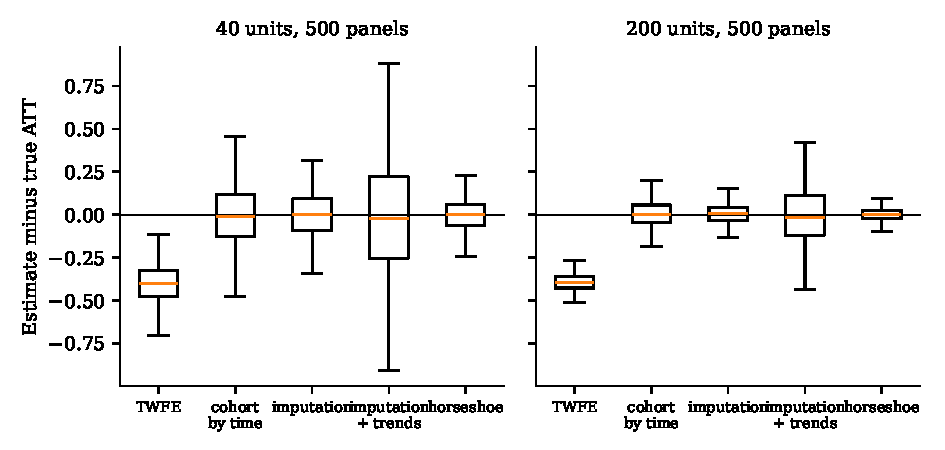
\includegraphics[width=\linewidth]{did_sim.pdf}
\caption{Estimate minus the true average effect on the treated for five estimators in 500 simulated staggered adoption panels of 40 units (left) and of 200 units (right), with effects growing with exposure and 10 percent of units departing from parallel trends. Boxes show quartiles; whiskers reach the most extreme estimate within 1.5 interquartile ranges of the box.}
\label{fig:didsim}
\end{figure}

\begin{table}[ht]
\centering
\caption{Simulation results for the average effect on the treated in the chapter's design (10 percent of units depart from parallel trends, effects growing with exposure): 500 panels per column group and the estimators on the same panels. Cohort by time uses never treated controls, Imputation is the estimator of Borusyak, Jaravel and Spiess (2024), the next row adds a linear trend for every unit, and Horseshoe is the estimator of this chapter. Coverage and width are for the 95 percent interval and are shown only for the estimators that have one. Monte Carlo standard errors are at most 0.015 for the biases and 0.013 for the coverages.}
\label{tab:didsim}
\footnotesize
\setlength{\tabcolsep}{4pt}
\begin{tabular}{@{}lcccccccc@{}}
\toprule
& \multicolumn{4}{c}{40 units} & \multicolumn{4}{c}{200 units} \\
\cmidrule(lr){2-5}\cmidrule(lr){6-9}
Estimator & Bias & RMSE & Cover & Width & Bias & RMSE & Cover & Width \\
\midrule
Two way fixed effects & $-$0.40 & 0.42 &  &  & $-$0.39 & 0.40 &  &  \\
Cohort by time & $-$0.01 & 0.18 &  &  & 0.00 & 0.08 &  &  \\
Imputation & 0.00 & 0.14 & 0.90 & 0.49 & 0.00 & 0.06 & 0.94 & 0.23 \\
Imputation, unit trends & $-$0.01 & 0.34 & 0.94 & 1.31 & 0.00 & 0.17 & 0.93 & 0.62 \\
Horseshoe & 0.00 & 0.09 & 0.98 & 0.42 & 0.00 & 0.04 & 0.97 & 0.18 \\
\bottomrule
\end{tabular}
\end{table}


\begin{table}[ht]
\centering
\caption{Root mean squared error of five estimators of the average effect on the treated over 500 panels per row, and coverage of the 95 percent interval of the three that have one. TWFE is two way fixed effects, Cohort the cohort by time estimator, Imput.\ the imputation estimator, Trend the imputation estimator with unit trends and HS the horseshoe. $N$ is the number of units, Dep the share of units whose trend departs from the common path, and the effect design is (a) the common path, (b) the path with one sparse cohort deviation, (c) the path with dense cohort deviations.}
\label{tab:didsimgrid}
\footnotesize
\setlength{\tabcolsep}{4pt}
\begin{tabular}{@{}rclcccccccc@{}}
\toprule
& & & \multicolumn{5}{c}{Root mean squared error} & \multicolumn{3}{c}{Coverage} \\
\cmidrule(lr){4-8}\cmidrule(lr){9-11}
$N$ & Dep & Design & TWFE & Cohort & Imput. & Trend & HS & HS & Imput. & Trend \\
\midrule
40 & 0.0 & (a) & 0.41 & 0.16 & 0.08 & 0.36 & 0.09 & 0.96 & 0.94 & 0.91 \\
40 & 0.0 & (b) & 0.37 & 0.15 & 0.08 & 0.37 & 0.09 & 0.96 & 0.94 & 0.90 \\
40 & 0.0 & (c) & 0.44 & 0.16 & 0.08 & 0.36 & 0.09 & 0.97 & 0.94 & 0.94 \\
\addlinespace
40 & 0.1 & (a) & 0.42 & 0.18 & 0.14 & 0.34 & 0.09 & 0.98 & 0.90 & 0.94 \\
40 & 0.1 & (b) & 0.39 & 0.18 & 0.13 & 0.35 & 0.09 & 0.98 & 0.93 & 0.93 \\
40 & 0.1 & (c) & 0.45 & 0.17 & 0.14 & 0.36 & 0.09 & 0.98 & 0.91 & 0.92 \\
\addlinespace
40 & 0.3 & (a) & 0.43 & 0.20 & 0.18 & 0.36 & 0.14 & 0.95 & 0.93 & 0.92 \\
40 & 0.3 & (b) & 0.39 & 0.21 & 0.19 & 0.35 & 0.15 & 0.94 & 0.90 & 0.93 \\
40 & 0.3 & (c) & 0.46 & 0.21 & 0.18 & 0.37 & 0.15 & 0.95 & 0.93 & 0.92 \\
\addlinespace
200 & 0.0 & (a) & 0.41 & 0.07 & 0.04 & 0.15 & 0.04 & 0.96 & 0.95 & 0.95 \\
200 & 0.0 & (b) & 0.37 & 0.07 & 0.04 & 0.17 & 0.04 & 0.96 & 0.93 & 0.93 \\
200 & 0.0 & (c) & 0.44 & 0.06 & 0.03 & 0.15 & 0.04 & 0.97 & 0.96 & 0.96 \\
\addlinespace
200 & 0.1 & (a) & 0.40 & 0.08 & 0.06 & 0.17 & 0.04 & 0.97 & 0.94 & 0.93 \\
200 & 0.1 & (b) & 0.37 & 0.08 & 0.06 & 0.15 & 0.04 & 0.96 & 0.94 & 0.96 \\
200 & 0.1 & (c) & 0.44 & 0.07 & 0.06 & 0.16 & 0.04 & 0.97 & 0.95 & 0.96 \\
\addlinespace
200 & 0.3 & (a) & 0.40 & 0.09 & 0.08 & 0.16 & 0.05 & 0.97 & 0.94 & 0.94 \\
200 & 0.3 & (b) & 0.37 & 0.09 & 0.08 & 0.16 & 0.05 & 0.97 & 0.94 & 0.95 \\
200 & 0.3 & (c) & 0.44 & 0.09 & 0.08 & 0.15 & 0.06 & 0.96 & 0.95 & 0.96 \\
\bottomrule
\end{tabular}
\end{table}


\begin{table}[ht]
\centering
\caption{Departures from parallel trends that go with adoption: 500 panels per block, effects growing with exposure (design (a)), the same five estimators on the same panels. In the first two blocks a unit departs with probability 0.3 if it adopts and never if it is never treated, so about 22 percent of all units depart; in the next two a unit departs with probability 0.1 if it adopts, so about 7.5 percent of units depart and all of them are treated; in the last two a unit departs with probability 0.3 if it is in the period 12 cohort and never otherwise. Bias and root mean squared error are for the average effect on the treated, coverage is for the 95 percent interval, and the last column is the mean of the squared error of the estimator minus that of the horseshoe on the same panel. Monte Carlo standard errors are in parentheses.}
\label{tab:didsimdep}
\footnotesize
\setlength{\tabcolsep}{4pt}
\begin{tabular}{@{}lcccc@{}}
\toprule
Estimator & Bias & RMSE & Cover & Squared error minus HS \\
\midrule
\multicolumn{5}{@{}l}{\emph{Adopters depart with probability 0.3, 40 units}} \\
Two way fixed effects & -0.222 (0.006) & 0.262 &  & 0.0479 (0.0040) \\
Cohort by time & 0.228 (0.008) & 0.285 &  & 0.0608 (0.0035) \\
Imputation & 0.259 (0.006) & 0.294 & 0.47 (0.02) & 0.0659 (0.0026) \\
Imputation, unit trends & -0.016 (0.016) & 0.367 & 0.92 (0.01) & 0.1141 (0.0090) \\
Horseshoe & 0.070 (0.006) & 0.144 & 0.93 (0.01) &  \\
\addlinespace
\multicolumn{5}{@{}l}{\emph{Adopters depart with probability 0.3, 200 units}} \\
Two way fixed effects & -0.216 (0.003) & 0.224 &  & 0.0450 (0.0013) \\
Cohort by time & 0.230 (0.003) & 0.243 &  & 0.0537 (0.0015) \\
Imputation & 0.263 (0.003) & 0.269 & 0.00 (0.00) & 0.0673 (0.0012) \\
Imputation, unit trends & -0.010 (0.007) & 0.157 & 0.94 (0.01) & 0.0194 (0.0018) \\
Horseshoe & 0.056 (0.002) & 0.072 & 0.87 (0.02) &  \\
\addlinespace
\multicolumn{5}{@{}l}{\emph{Adopters depart with probability 0.1, 40 units}} \\
Two way fixed effects & -0.335 (0.005) & 0.352 &  & 0.1151 (0.0034) \\
Cohort by time & 0.088 (0.007) & 0.175 &  & 0.0221 (0.0018) \\
Imputation & 0.090 (0.005) & 0.139 & 0.84 (0.02) & 0.0108 (0.0009) \\
Imputation, unit trends & -0.003 (0.016) & 0.352 & 0.95 (0.01) & 0.1156 (0.0082) \\
Horseshoe & 0.016 (0.004) & 0.092 & 0.97 (0.01) &  \\
\addlinespace
\multicolumn{5}{@{}l}{\emph{Adopters depart with probability 0.1, 200 units}} \\
Two way fixed effects & -0.341 (0.002) & 0.345 &  & 0.1170 (0.0015) \\
Cohort by time & 0.078 (0.003) & 0.107 &  & 0.0097 (0.0005) \\
Imputation & 0.086 (0.002) & 0.098 & 0.58 (0.02) & 0.0079 (0.0004) \\
Imputation, unit trends & -0.003 (0.007) & 0.164 & 0.94 (0.01) & 0.0251 (0.0017) \\
Horseshoe & 0.010 (0.002) & 0.042 & 0.97 (0.01) &  \\
\addlinespace
\multicolumn{5}{@{}l}{\emph{Period 12 cohort departs with probability 0.3, 40 units}} \\
Two way fixed effects & -0.353 (0.005) & 0.369 &  & 0.1285 (0.0034) \\
Cohort by time & 0.015 (0.007) & 0.151 &  & 0.0153 (0.0012) \\
Imputation & -0.014 (0.004) & 0.087 & 0.93 (0.01) & -0.0000 (0.0003) \\
Imputation, unit trends & -0.008 (0.016) & 0.359 & 0.92 (0.01) & 0.1211 (0.0092) \\
Horseshoe & -0.002 (0.004) & 0.087 & 0.98 (0.01) &  \\
\addlinespace
\multicolumn{5}{@{}l}{\emph{Period 12 cohort departs with probability 0.3, 200 units}} \\
Two way fixed effects & -0.364 (0.002) & 0.367 &  & 0.1330 (0.0015) \\
Cohort by time & 0.023 (0.003) & 0.070 &  & 0.0034 (0.0003) \\
Imputation & -0.020 (0.002) & 0.041 & 0.93 (0.01) & 0.0002 (0.0001) \\
Imputation, unit trends & 0.008 (0.007) & 0.153 & 0.96 (0.01) & 0.0220 (0.0014) \\
Horseshoe & -0.001 (0.002) & 0.038 & 0.99 (0.00) &  \\
\bottomrule
\end{tabular}
\end{table}


 Two way fixed effects is biased downward by 0.40 at 40 units and 0.39 at 200, about 36 percent of the average effect of 1.12: the negative weighting problem at work, and more units do not remove it. The cohort by time estimator removes that bias. Its root mean squared error is 0.18 at 40 units and 0.078 at 200, against 0.092 and 0.040 for the horseshoe, and the paired differences in squared error, 0.024 and 0.0045 with Monte Carlo standard errors 0.002 and 0.0004, are many standard errors from zero. The horseshoe's 95\% intervals cover the truth in 98 and 97 percent of panels, and in 94 to 98 percent in all 18 settings of Table~\ref{tab:didsimgrid}, whose departures are independent of adoption.

The imputation estimator shows where the gain comes from. With no departures it is as accurate as the horseshoe or slightly more (root mean squared error 0.082 against 0.088 at 40 units, 0.035 against 0.038 at 200), so there the advantage over the cohort by time estimator (0.159 and 0.066) comes from using every untreated observation rather than one base period. Departures are independent of adoption and add noise through differing shares of diverging units among adopters and controls, without biasing imputation (absolute bias at most 0.012 in all 18 settings). With 10 percent departures its error rises to 0.139 and 0.059, its intervals cover in 90 and 94 percent of panels, and the horseshoe is ahead by 0.011 and 0.0019 in squared error, with Monte Carlo standard errors 0.001 and 0.0002; with 30 percent departures the gap is wider, 0.18 against 0.14 at 40 units and 0.08 against 0.05 at 200. That remaining gain comes from shrinking the trend departures: the horseshoe gives the few diverging units their own trends and holds the rest on the common path. Giving every unit its own unshrunk trend in the imputation estimator absorbs the departures too, but raises its root mean squared error to 0.34 and 0.17, about two and a half to three times that of the imputation estimator without trends.

The sparse and dense cohort deviations of designs (b) and (c) change none of these comparisons: at a given panel size and share of departures, the root mean squared error of each estimator other than two way fixed effects moves by at most 0.022 across the three designs.

In the 18 settings the departing units are drawn independently of adoption. Table~\ref{tab:didsimdep} drops that assumption in three further designs, with the same departure trend $0.15(t-8)$, the effects of design (a), the same five estimators and 500 panels at each of 40 and 200 units. In the first, a unit departs with probability 0.3 if it adopts and never if it is never treated, so about 22 percent of all units depart and every one of them is treated. The second is the same with probability 0.1, so about 7.5 percent of units depart, again all of them adopters. In the third, only units of the period 12 cohort depart, each with probability 0.3, about 7.5 percent of all units.

When the adopters depart, the imputation estimator is biased upward by 0.26, about a quarter of the average effect, at both sizes; cohort by time and two way fixed effects are biased too, by 0.23 and $-0.22$. The horseshoe has half the root mean squared error of the imputation estimator or less (0.144 against 0.294 at 40 units, 0.072 against 0.269 at 200), but it is biased as well, by 0.070 at 40 units and 0.056 at 200 with Monte Carlo standard errors 0.006 and 0.002. The bias barely falls with the sample size, and at 200 units it makes up about 60 percent of the horseshoe's mean squared error. Refitting the same panels traces the bias to shrinkage: departing units' posterior mean trends are 0.85 of truth at 40 units and 0.87 at 200. Each trend uses its unit's 16 periods, so more units do not sharpen it. Four times as many sweeps leave the bias unchanged to three decimals. A fit that gives unshrunk trends only to the known departing units is unbiased ($-0.001$ and 0.000) and covers in 96 and 97 percent of panels, ruling out sampler and identification failures.

The horseshoe's intervals cover in 93 percent of panels at 40 units and 87 percent at 200, below the 94 to 98 percent of the 18 settings. The imputation estimator's interval covers the truth in 47 percent of panels at 40 units and in 1 of 500 at 200. Imputation with unshrunk unit trends is nearly unbiased ($-0.016$ and $-0.010$) and covers in 92 and 94 percent of panels, at a root mean squared error of 0.367 and 0.157, two and a half and two times the horseshoe's.

With departure probability 0.1 the shrinkage costs much less. The horseshoe's bias falls to 0.016 at 40 units and 0.010 at 200 (standard errors 0.004 and 0.002), its intervals cover in 97 percent of panels at both sizes, and its root mean squared error, 0.092 and 0.042, is a third and more than half below that of the imputation estimator, which is biased by 0.09 and covers in 84 and 58 percent. This is the case the horseshoe on departures is built for, a few units leaving the common trend, and it is the most accurate of the five estimators there.

When only the period 12 cohort departs, the imputation estimator is nearly unbiased ($-0.014$ and $-0.020$) and the horseshoe gains nothing: the two have the same root mean squared error, 0.087, at 40 units, and 0.038 against 0.041 at 200. There the horseshoe's intervals cover in 98 and 99 percent of panels and the imputation estimator's in 93.

\section{Application: castle doctrine laws and homicide}

Between 2005 and 2010 over twenty American states adopted castle doctrine laws\index{castle doctrine laws|textbf}, which extend the right to use lethal force in self defense beyond the home and remove the duty to retreat. Cheng and Hoekstra (2013) used the staggered adoption to estimate a homicide increase of roughly eight percent\index{castle doctrine laws!homicide|textbf}. Their data, distributed with Cunningham's \emph{Mixtape} (Cunningham 2021), cover 50 states from 2000 to 2010.

Here 21 states adopt within the sample: one in 2006, thirteen in 2007, four in 2008, two in 2009 and one in 2010, with adoption dated by the first year the post law indicator equals one; for Florida, whose law took effect in October 2005, that is 2006. Figure~\ref{fig:castleraw} shows mean log homicide rates for never adopting states, the 2006 adopter and later adopters.

\begin{figure}[ht]
\centering
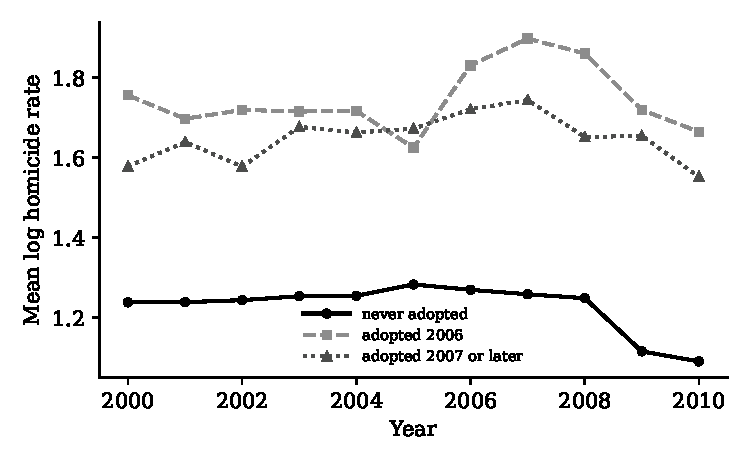
\includegraphics[width=\linewidth]{castle_raw.pdf}
\caption{Mean log homicide rate per 100,000 in never adopting states, the 2006 adopter and the states adopting in 2007 or later, 2000 to 2010.}
\label{fig:castleraw}
\end{figure}

\begin{table}[ht]
\centering
\caption{Effect of castle doctrine laws on the log homicide rate.}
\label{tab:castle}
\small
\begin{tabular}{lcc}
\toprule
Estimator & Estimate & Interval \\
\midrule
Two way fixed effects & 0.069 & \\
Cohort by time, never treated controls & 0.019 & \\
Horseshoe difference in differences, equal noise & 0.025 & [$-$0.046, 0.096] \\
\addlinespace
Two way fixed effects, population weights & 0.076 & \\
Horseshoe, population weights & 0.079 & [0.027, 0.129] \\
\bottomrule
\end{tabular}
\end{table}


Unweighted two way fixed effects\index{two way fixed effects!in the castle data|textbf} on log homicide gives 0.069, close to the published estimate. The cohort by time estimator gives 0.019. With four chains of 20,000 sweeps from dispersed starts, discarding the first 5,000 of each, the horseshoe gives posterior mean 0.025, 95\% interval $-0.046$ to $0.096$, and posterior probability 0.76 of a positive effect. Figure~\ref{fig:castle} shows the event study and the posterior.

\begin{figure}[ht]
\centering
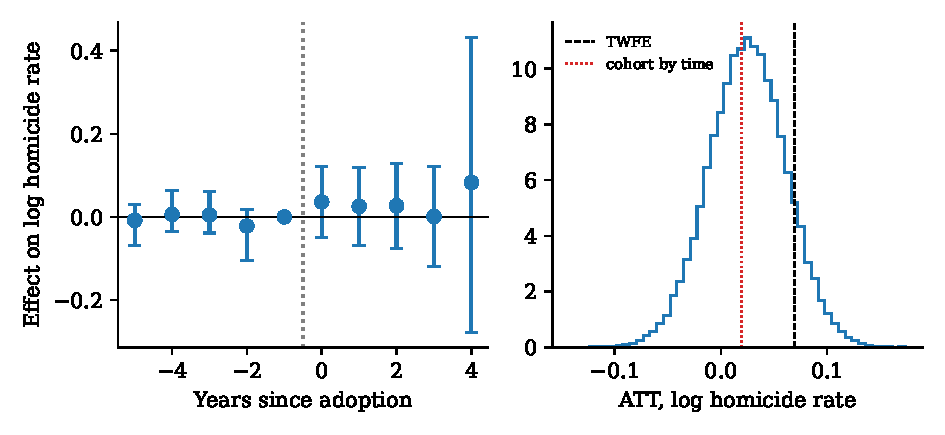
\includegraphics[width=\linewidth]{castle.pdf}
\caption{Left: horseshoe event study for castle doctrine laws, posterior means and 95\% intervals; leads are shrunk by their own horseshoe and the period before adoption, with all periods more than five years before, is the reference. Right: posterior of the average effect on the treated, with the two way fixed effects and cohort by time estimates.}
\label{fig:castle}
\end{figure}

The leads are close to zero, but they measure shrunk departures beyond the modelled state trends and cannot be read as support for parallel trends. The post adoption path is positive but imprecise; the effect four years out rests on one state and is very uncertain. The largest absolute posterior mean of a state trend departure is about 0.5 on the log scale per standard deviation of the year index (3.2 years), so a few states do diverge.

With flat priors on the leads and the rest of the model unchanged, the lead at $e = -2$ is $-0.064$ (95\% interval $-0.16$ to 0.03), the effect on the treated is 0.013 and the probability that it is positive is 0.63; with the horseshoe on the leads the same three numbers are $-0.024$, 0.023 and 0.74. These two fits, and the fit without trends below, each run one chain of 4,000 sweeps, discard the first 1,000 and start from the same fixed seed. The horseshoe lead fit uses the model of Figure~\ref{fig:castle}; 0.74 is about two Monte Carlo standard errors from the four chain fit's 0.76 (standard errors about 0.01 and 0.002, respectively). Flat leads and dropping the trend block change the model, so their differences from 0.76 are not Monte Carlo error.

The four chains agree: the effect on the treated has split $\hat R=1.0003$ and effective sample sizes of about 26,000 for its mean and 34,000 for the indicator that it is positive; Monte Carlo standard errors are 0.0002 for the mean and 0.0004 for each end of the interval. Errors within a state may be serially correlated, which Bertrand, Duflo and Mullainathan (2004) show makes the usual standard errors too small. Refitting with AR(1) errors within each state, correlation $\rho^{|t-s|}$ between years $t$ and $s$ and a uniform prior on $\rho$ over $(-1, 1)$, again with four chains of 20,000 sweeps, gives a posterior mean of 0.06 for $\rho$ (95\% interval $-0.06$ to 0.18), an effect on the treated of 0.023 with interval $-0.051$ to 0.095, and probability 0.73 that it is positive. Little serial correlation is left once the state effects and trends are in the model, and the conclusion does not move.

What moves the estimate, in this model with equal noise in every state, is the trend departure block. Refitting the horseshoe model without it, with the same path, cohort deviations and leads, gives 0.067 with 95\% interval 0.000 to 0.133 and probability 0.97 that the effect is positive, essentially the two way fixed effects value of 0.069. Cohort heterogeneity alone barely changes the estimate: all 15 two way fixed effects cell weights are positive and the posterior event path does not grow with exposure, so the simulation's 36 percent bias does not carry over. The cohort by time estimate of 0.019 is low because it uses one base period and only never treated controls, so it agrees with the horseshoe's 0.025 for different reasons. Cheng and Hoekstra's specification also included covariates and population weights, and the weights change the answer. The log of the squared residual falls with slope about $-1$ on log population, so equal noise across states does not fit these data. Refitting with $\mathrm{Var}(\varepsilon_{it}) = \sigma^2/w_i$, where $w_i$ is the state's average population over the panel relative to the mean of these averages, gives 0.079 with 95\% interval 0.027 to 0.129 and probability 0.998 that the effect is positive, close to the published eight percent, and adding their covariates gives 0.084; the covariates alone change almost nothing (Exercise~\ref{ex:chdid:3}). So the reading of about three to one, with a central estimate a third of the two way fixed effects coefficient, holds only under equal noise. Under the noise model the residuals support, allowing departures from parallel trends leaves Cheng and Hoekstra's estimate standing. It does lean on a few large adopters: dropping the single 2006 adopter gives 0.049 and probability 0.96.

No number of pre adoption periods can separate an effect from an adopter specific shock that starts at adoption: adding a constant $a$ to the untreated outcomes of adopters in every post adoption period and subtracting $a$ from every post adoption effect leaves the observed data unchanged. The model assumes no such shocks and that each unit's linear trend continues unchanged after adoption; the castle posterior mean of 0.025 depends on extrapolating the estimated state trends past adoption. Rambachan and Roth (2023) bound post adoption departures relative to pre adoption ones, for example by limiting changes in slope between adjacent periods to $M$ ($M = 0$ gives a linear departure). They report the set of compatible effects, with confidence sets accounting for estimated pre trends. These are frequentist sensitivity results, not posterior intervals under one model. The Bayesian counterpart is a prior on the post adoption change in slope.

\section{Relation to synthetic control}

Synthetic control\index{synthetic control|textbf} (Abadie and Gardeazabal 2003; Abadie, Diamond and Hainmueller 2010) builds a treated unit's counterfactual as a weighted average of controls matching its pre treatment path. It complements difference in differences when few units are treated and parallel trends is doubtful. Nonnegative weights summing to one keep the counterfactual within the donors' range and usually give only a few donors positive weight. A horseshoe on the weights likewise says few controls matter, but the weights may then be negative and need not sum to one, so the counterfactual can extrapolate beyond the donors. The trend departure $\delta_i$ in \eqref{eq:hsdid0} is a one factor model with a unit specific loading on time.

The two designs answer the same question with different information. Difference in differences borrows the common period effects $\gamma_t$ from every control unit and each adopter supplies its own level $\alpha_i$ and trend; synthetic control uses one adopter's pre treatment path to choose controls and uses those alone. With many adopters and a common untreated time effect, the first is more efficient; for one adopter whose path looks like no average, such as California in the tobacco study of Abadie, Diamond and Hainmueller (2010), the second is more credible. The horseshoe formulation makes the choice one of model and prior. For one adopter $i$ and controls $j$, synthetic control fits $Y_{it} = \sum_j w_j Y_{jt} + \varepsilon_{it}$ for $t < G_i$, with a horseshoe on the weights $w_j$. The factor model in Exercise~\ref{ex:chdid:4} uses two latent factors, their number fixed by the analyst, with a horseshoe on the loadings so most units load little and a few heavily. These two models and the trend departures $\delta_i$ give three sparsity judgements about departures from two way additivity; each gives a posterior counterfactual path for every adopter, from which the effect on the treated is an accounting. In all three, check the pre adoption residuals: shrunken leads can look flat despite poor fit, and even close pre adoption fit cannot show that the relation holds afterwards.

\section{In practice}

\paragraph{The target.} The targets are the average effect on the treated, the event study path, and the effect for each cohort, each a weighted sum of the draws of $\theta_e + u_{g,e}$ over the relevant cells. The posterior probability that an effect is positive, 0.76 for castle doctrine laws, is the fraction of draws in which the weighted sum exceeds zero.

\paragraph{What the analyst does differently.} The analyst writes down the cohort by event time matrix before estimating anything and notes which cells rest on little data: in the castle doctrine data thirteen of the 21 adopting states fall in the 2007 cohort, and the effect four years out rests on one state. She fits the horseshoe model with the path $\theta_e$ unpenalized and reports from one posterior the event study with its leads, checked against the pre adoption residuals because the leads are shrunk; the effect on the treated with its interval; the probability of a positive effect; and the largest trend departure, so the reader knows that a few states diverge and that the model let them. She reports the two way fixed effects coefficient alongside, not as the answer, with the fit without the trend block that accounts for the gap between them.

\paragraph{Against DML.} DML is not the natural competitor in this chapter. The modern difference in differences estimators of Callaway and Sant'Anna (2021), de Chaisemartin and D'Haultf\oe uille (2020), Sun and Abraham (2021) and Borusyak, Jaravel and Spiess (2024) are the right comparison, and some of them use doubly robust scores in the DML spirit when covariates enter. On the average effect under parallel trends they are adequate: in the simulation with no trend departures the imputation estimator was unbiased, as accurate as the horseshoe and faster. Giving every unit its own unshrunk trend cost two and a half to three times the error when 10 percent of units departed independently of adoption. When 22 percent of units departed, all of them adopters, the estimators without unit trends were biased by 0.22 to 0.26 in absolute value and the horseshoe by 0.06 to 0.07; the version with unshrunk trends kept its intervals close to nominal at both panel sizes, at two to two and a half times the horseshoe's error. When 7.5 percent departed with adoption, the horseshoe's bias fell to 0.01 or 0.02 and its error was the lowest of the five estimators. Nor do they give the probability of a positive effect, and the leads are tested rather than modelled. Where the analyst needs to say how strong the evidence is, as the castle doctrine data require, the posterior gives that directly.

\section*{Notes}

Three papers show the negative weights of two way fixed effects from different sides. Goodman Bacon (2021) splits the coefficient into two by two comparisons, some of which use units that are already treated as controls, de Chaisemartin and D'Haultf\oe uille (2020) write it as a weighted sum of cohort by period effects, and Sun and Abraham (2021) show that event study coefficients from the same regression pick up effects from other event times. Roth, Sant'Anna, Bilinski and Poe (2023) survey the recent literature.

The horseshoe is from Carvalho, Polson and Scott (2010), and the sources for its theory are in the Notes of Chapter~\ref{ch:critique}. The idealized rates in Appendix~\ref{app:guarantees} use van der Pas, Kleijn and van der Vaart (2014) and van der Pas, Szab\'o and van der Vaart (2017a), with the minimax lower bound of Donoho, Johnstone, Hoch and Stern (1992).

Arkhangelsky and coauthors (2021) combine synthetic control with difference in differences, and Brodersen and coauthors (2015) build the counterfactual path with a Bayesian structural time series model. The chapter takes adoption to be absorbing and covariates to be absent, and its simulations take errors to be independent. Callaway and Sant'Anna (2021) allow covariates and de Chaisemartin and D'Haultf\oe uille (2020) let treatment switch on and off. The targets here are means. For continuous outcomes, the changes in changes model of Athey and Imbens (2006) writes untreated outcomes as $h_t(U)$, with $h_t$ common to both groups and strictly increasing in the scalar $U$. If the distribution of $U$ is stable over time within each group and the adopters' latent support is contained in the controls' support, the model identifies the adopters' counterfactual outcome distribution and quantile effects on the treated.

\begin{exercises}
\item\label{ex:chdid:1} Compute the two way fixed effects weights $\omega_{g,e}$ in a balanced panel with periods 1 to 8, two cohorts of any sizes that first adopt in periods 3 and 6, and no never treated units, and identify the negative weights.
\item\label{ex:chdid:2} Show that the cohort by time estimator with never treated controls and base period $g - 1$ is unbiased for $\tau_{g,e}$ under parallel trends, and biased by $(t - g + 1)/s_t$ times the average of $\delta_i$ over the cohort under the trend departure model, where $s_t$ is the standard deviation used to standardize time and the departures average zero over the never treated units.
\item\label{ex:chdid:3} Refit the castle doctrine model with population weights and the covariates used by Cheng and Hoekstra and compare the posterior with the equal noise rows of Table~\ref{tab:castle}.
\item\label{ex:chdid:4} Replace the horseshoe on trend departures with a horseshoe on loadings in a two factor model with latent factors $f_t \in \R^2$ with prior $N(0, I_2)$ and unit loadings $\delta_i \in \R^2$, and derive the Gibbs sampler.
\item\label{ex:chdid:5} Construct a simulation in which the original single effect parametrization of the horseshoe estimator fails and the path parametrization succeeds, and explain the result in terms of sparsity.
\end{exercises}

\chapter{Two Benchmarks}\label{ch:k401}

\begin{tcolorbox}[colback=gray!6,colframe=gray!50,title=In brief,fonttitle=\normalfont\itshape,coltitle=black,colbacktitle=gray!15,boxrule=0.4pt,arc=1pt]
On the 401(k) data the flexible methods that report one effect for everyone, DML and the horseshoe, put it between 8.6 and 9.8 thousand dollars, while least squares with nine covariates gives 5.9. The posterior adds what that one effect hides: effects of one or two thousand dollars at low incomes and about 21 thousand at the top, and an effect on the untreated 40 percent smaller than on the treated. On the LaLonde benchmark the experiment gives 1.79; the raw difference with survey controls is $-8.50$, least squares gives 1.07, and the flexible methods give 1.39 to 1.68.
\end{tcolorbox}

We compare DML and Bayesian estimates of the effect of 401(k) eligibility\index{401(k) plan} on household net financial assets, using the 1991 wave of the Survey of Income and Program Participation, the leading empirical example of Chernozhukov et al. (2018). All estimates come from our own analysis; the scripts are in the repository of Appendix~\ref{app:code}.

\section{The question and the data}

A worker is eligible for a 401(k) plan\index{401(k) plan!eligibility and participation|textbf} if her employer offers one. Following Poterba, Venti and Wise (1995), we assume eligibility is close to randomly assigned given the covariates (Section~\ref{sec:dml:k401}).

The sample has 9,915 households. The outcome is net total financial assets, in thousands of dollars. The treatment is eligibility, held by 37\% of households. The covariates are age, income, years of education, family size, and indicators for marriage, two earner households, a defined benefit pension, an individual retirement account and home ownership. We expand the nine covariates into 54 standardized terms: the covariates, their squares and pairwise interactions. The five binary squares are affine in their indicators, leaving 49 effective terms.

The outcome is highly skewed, with median about 1.5 thousand dollars and maximum over 1.5 million. 

\section{Estimates of the average effect}

Table~\ref{tab:k401} collects the estimates. Least squares with nine covariates and DML with forests use the covariates as they are, and the other adjusted rows use the 54 term basis. The lasso plug in regresses assets on eligibility and the 54 terms with one lasso penalty on every coefficient, eligibility included, chosen by five fold cross validation. The horseshoe rows keep 2,000 Gibbs draws, and the coupled prior takes its propensity from a cross validated logistic regression on the basis. The DML rows show one random partition of the data.

\begin{table}[ht]
\centering
\caption{Estimates of the effect of 401(k) eligibility on net financial assets, thousands of dollars. Intervals are 95\% confidence intervals for DML and 95\% posterior intervals for the Bayesian methods. The DML rows use the partially linear score and the regression and horseshoe rows assume a constant effect, so with flexible adjustment and varying effects each estimates the average of $\tau(x)$ weighted by $e(x)\{1 - e(x)\}$.}
\label{tab:k401}
\small
\begin{tabular}{lcc}
\toprule
Method & Estimate & Interval \\
\midrule
Difference in means & 19.56 & \\
Least squares, nine covariates & 5.90 & \\
Least squares, 54 term basis & 9.84 & \\
Lasso plug in, 54 term basis & 8.89 & \\
DML, random forests & 8.59 & [6.05, 11.12] \\
DML, lasso on 54 term basis & 9.52 & [6.89, 12.14] \\
Horseshoe, independent prior & 9.79 & [7.45, 12.07] \\
Horseshoe, coupled to propensity & 9.82 & [7.42, 12.11] \\
\bottomrule
\end{tabular}
\end{table}

Adjustment matters a great deal. The raw difference of 19.6 thousand dollars is driven by eligible households having higher incomes, and higher income households saving more. Every adjusted estimate is about half of it or less.

Functional form matters too. Least squares with the nine covariates entering linearly gives 5.9; with the 54 term basis, 9.8. Income and assets are strongly nonlinearly related, and a linear adjustment leaves confounding behind.

With flexible enough adjustment the methods that report one effect for everyone agree: DML with forests or the lasso and both horseshoes\index{horseshoe prior} give 8.6 to 9.8 thousand dollars, with intervals about 5 thousand dollars wide. Posterior standard deviations, about 1.2, are close to the DML standard errors, about 1.3.

Regularization induced confounding\index{regularization induced confounding} did not bite: the independent and coupled horseshoe posteriors are nearly identical. With almost ten thousand observations and 54 basis terms, the likelihood dominates the prior for the important coefficients, and tail robustness\index{tail robustness} should leave the large coefficients lightly shrunk. The simulation of Section~\ref{sec:ricsim}, with $n = 200$ and $p = 50$, found that coupling cut the independent horseshoe's bias from 0.059 to $-0.023$; here $n$ is large relative to $p$, and the priors coincide. 

\paragraph{Sample splitting variability.} Over 20 random partitions\index{cross fitting!variance from the random split}, lasso DML estimates range from 9.52 to 10.26 (median 9.84, standard deviation 0.17); over 5 partitions, forest estimates range from 8.59 to 9.05 (median 9.00, standard deviation 0.21). The table's partition happens to give the lowest estimate for both learners; Chernozhukov et al. (2018) recommend reporting the median. These ranges are small relative to the standard errors but not zero: two analysts with the same data and method, differing only in a random seed, report estimates up to 0.7 thousand dollars apart. The posterior has a spread of its own, the Monte Carlo error of the Gibbs sampler. For the independent horseshoe the 2,000 draws of the treatment coefficient are nearly independent (Section~\ref{comp:sec:cost}), so with posterior standard deviation 1.19 the error is about $1.19/\sqrt{2{,}000} \approx 0.03$ thousand dollars. It shrinks with the number of draws, whereas the partition spread is fixed by the design and invisible in any single run. An analyst should report the spread across partitions with a DML estimate and the Monte Carlo error with a posterior mean.

\section{Heterogeneity and accounting}\label{sec:k401acc}

The average hides large differences by income\index{401(k) plan!heterogeneity by income|textbf}\index{heterogeneous treatment effects!by income|textbf}. We let the effect of eligibility in the coupled horseshoe model differ across income quintiles\index{income quintile|textbf}, with the five quintile specific effects unpenalized and the rest unchanged. Figure~\ref{fig:k401} shows the posteriors.

\begin{figure}[ht]
\centering
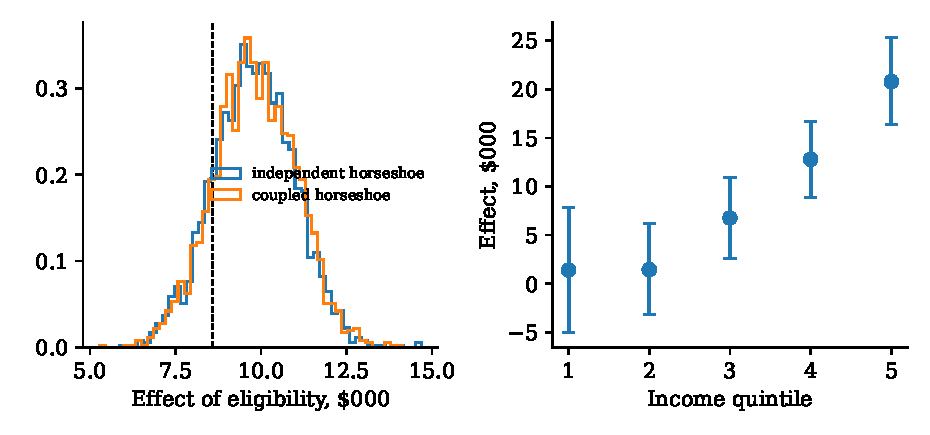
\includegraphics[width=\linewidth]{k401.pdf}
\caption{Left: posteriors of the average effect under the independent and coupled horseshoe priors; the dashed line is the DML forest estimate. Right: posterior means and 95\% intervals for the effect of eligibility by income quintile.}
\label{fig:k401}
\end{figure}

\begin{table}[ht]
\centering
\caption{Posterior effect of eligibility by income quintile, thousands of dollars.}
\label{tab:k401q}
\small
\begin{tabular}{lccc}
\toprule
Income quintile & Mean & Standard deviation & 95\% interval \\
\midrule
1 (lowest) & 1.41 & 3.39 & [$-5.04$, 7.87] \\
2 & 1.45 & 2.44 & [$-3.14$, 6.22] \\
3 & 6.76 & 2.08 & [2.59, 10.89] \\
4 & 12.80 & 2.01 & [8.87, 16.68] \\
5 (highest) & 20.78 & 2.23 & [16.39, 25.34] \\
\bottomrule
\end{tabular}
\end{table}

The effect rises steeply with income, from about 1.4 thousand dollars in the bottom two quintiles, with intervals including zero, to about 21 thousand at the top. Small low income effects could reflect low take up of the plan or substitution for other saving; an analysis of eligibility alone cannot distinguish them.

Weighting the quintile effects by each quintile's share in a chosen population, the same posterior draws give three averages:
\begin{itemize}
\item Over all households: 8.64, with 95\% interval [6.21, 11.17].
\item Over eligible households, the effect on the treated: 11.65, with interval [9.27, 14.16].
\item Over ineligible households, the effect on the untreated\index{effect on the treated!and untreated|textbf}: 6.86, with interval [4.12, 9.62].
\end{itemize}
The effect on the treated\index{effect on the treated} is larger because eligible households are richer. A policymaker considering extending eligibility to ineligible workers needs the third number, about 40\% smaller than the effect on the treated. All three come from one fit.

Each accounting is a weighted average of the five quintile means of Table~\ref{tab:k401q}. The weights are 0.2 for every quintile over all households; 0.07, 0.14, 0.21, 0.26 and 0.32 over eligible households; and 0.28, 0.23, 0.20, 0.16 and 0.13 over ineligible households. The last two vectors are the shares of each group in the five income quintiles, which follow from eligibility rates of 13, 26, 38, 49 and 59 percent by quintile. Because the weights are rounded, a hand computation reproduces 8.64 exactly but moves 11.65 and 6.86 by up to 0.05.

The $e(x)\{1 - e(x)\}$ weights in the caption of Table~\ref{tab:k401} favour households where eligibility is closest to a coin flip. Their means in the five income quintiles are 0.135, 0.183, 0.213, 0.233 and 0.230, so the lowest two quintiles, with the smallest effects, count less. Applied to the means of Table~\ref{tab:k401q}, these weights give 9.71, close to the 9.5 to 9.8 of lasso DML and the horseshoes, against 8.64 with equal weights. The gap of about 1.1 thousand dollars is a difference of estimand. The forest estimate, 8.59, targets the same weighted average with different nuisance fits.

DML can also report the quintile effects. Averaging the augmented inverse propensity weighted score over the households of each quintile, with the two outcome regressions and the propensity fitted once per partition (five folds, the 54 term basis for the lasso and the nine covariates for the forests, propensities clipped at 0.01 and 0.99) and the median taken over 100 random partitions, gives 3.86, 1.27, 5.55, 10.43 and 21.04 thousand dollars with the lasso, with 95\% intervals [2.33, 5.39], [$-1.87$, 4.40], [3.01, 8.10], [5.84, 15.02] and [10.78, 31.30], and 4.36, 0.83, 5.05, 10.62 and 19.63 with forests. Every estimate lies inside the matching horseshoe interval of Table~\ref{tab:k401q}, the second quintile interval contains zero for both learners, and the same score averaged over all households gives 8.42 with the lasso and 8.08 with forests, against the posterior's 8.64. The DML intervals are narrower than the posterior's in the three lowest quintiles and wider in the two highest, most of all at the top, where the standard error is 5.2 against a posterior standard deviation of 2.2. Clipping touched at most 2 households in a partition with the lasso, in the first, second and fifth quintiles, and at most 66 with forests, all in the lowest quintile.

\section{A tree based check: Bayesian causal forest}

We tried a Bayesian causal forest\index{Bayesian causal forest}\index{Bayesian causal forest!in the 401(k) data|textbf} to check the horseshoe's chosen basis and income quintiles. It learns functional form and heterogeneity from the nine raw covariates, with the estimated propensity in its prognostic forest. Eight chains of 50,000 retained draws each did not converge: for the average effect, split $\hat R$ is 1.19 and effective sample size 27; in the top income decile, 1.64 and 13, with chain means from 13 to 25 thousand dollars. Draws from chains that disagree this much are not a posterior, so we report no forest estimates; the income profile check by a second model class remains to be done.

\section{Overlap and the outcome distribution}\label{sec:k401overlap}

Estimated eligibility propensities range from 0.02 to 0.89. Overlap\index{overlap!in the 401(k) data|textbf}\index{401(k) plan!overlap|textbf} is adequate but thin at low incomes, where eligible households are scarce. Weighting estimators give those households large weights; the outcome model pools across nearby incomes. The bottom quintile interval of Section~\ref{sec:k401acc}, $-5.04$ to 7.87, is nearly one and a half times as wide as the top quintile's: the posterior reports the scarcity as uncertainty, whereas a few large weights inflate the variance of the average without saying where the thinness is.

Skewness of the outcome\index{401(k) plan!outcome distribution|textbf} is more serious for every method: a few wealthy households strongly influence both the Gaussian horseshoe fit and DML's squared error nuisance regressions. Student $t$ errors, a scale mixture of normals, slot into the Gibbs sampler of Chapter~\ref{ch:horseshoe}; quantile models address the distribution directly (Chapter~\ref{ch:gente}). Chernozhukov and Hansen's (2004) instrumental quantile analysis of these data, estimating the effect of participation instrumented by eligibility, found the effect concentrated in the upper part of the asset distribution, consistent with the income pattern above. DML has no error model to check.

Figure~\ref{fig:ppc401k} gives a posterior predictive check of the coupled horseshoe of Table~\ref{tab:k401} on 9,915 households, fitted once with Gaussian errors and once with Student $t$ errors\index{Student t errors|textbf} on three degrees of freedom (3,000 sweeps each, 1,000 discarded). From each fit we take 1,000 posterior draws and replicate the outcome once per draw at the observed covariates and eligibility, with the draw's error scale and, for the $t$ model, latent weights drawn afresh from their prior. Neither model passes. The Gaussian replicates match the mean and standard deviation of net financial assets but are far too symmetric: the observed 5th percentile is $-9$ thousand dollars and the median 1.5 thousand, against replicated values of $-77$ (95\% range $-80$ to $-74$) and 15 (13 to 17), and the observed skewness is 10.6 against 0.9. The $t$ replicates are closer in the lower tail and the centre, with a 5th percentile of $-19$ and a median of 5.6, but their upper tail is far too light (95th percentile 53 against 92, 99th 87 against 220), and their mean, 9.6 against the observed 18.1, shows that the $t$ model describes the centre of the distribution and not its average. For both models the observed quantile lies outside the 95\% range at 95 of the 99 levels from 0.01 to 0.99. Assets are also more dispersed among eligible households than among ineligible ones (standard deviations 74.8 and 54.5 thousand dollars), which one error scale for everyone cannot reproduce.

\begin{figure}[ht]
\centering
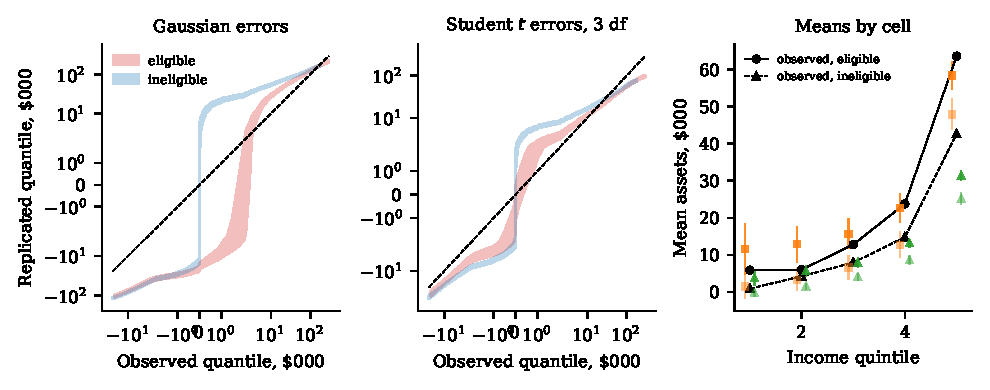
\includegraphics[width=\linewidth]{ppc401k_post.pdf}
\caption{Posterior predictive check of the coupled horseshoe for the 401(k) data, 1,000 posterior draws and one replicated data set from each. Left and middle: 95\% ranges of replicated quantiles (levels 0.01 to 0.99) against observed quantiles, on a symmetric log scale, for eligible and ineligible households, with Gaussian errors (left) and Student $t$ errors on three degrees of freedom (middle). Right: observed mean assets by income quintile (eligible solid, ineligible dashed) with replicated means and 95\% ranges (squares Gaussian, triangles $t$; eligible dark, ineligible light).}
\label{fig:ppc401k}
\end{figure}

The Student $t$ refit uses three degrees of freedom and a sampled scale. Each household has a latent weight $w_i \sim \mathrm{Gamma}(3/2, 3/2)$ and error variance $\sigma^2/w_i$, and each Gibbs sweep adds a draw of the weights given the residuals to the sampler of Table~\ref{tab:k401} (3,000 sweeps, the first 1,000 discarded; split $\hat R$ of 1.002 over four chains). The common effect falls from 9.82 to 4.22, with 95\% interval [3.68, 4.73], and the equal weight average of the five quintile effects falls from 8.64 to 4.83. The $t$ model has not found that eligibility raises mean assets by less. It measures a different location. Net financial assets are strongly skewed to the right, and a likelihood that discounts large residuals fits a line nearer the centre of the conditional distribution than its mean; with symmetric errors the two fits would agree (Exercise~\ref{ex:chk401:1}). In a typical draw 9 percent of households carry a weight below 0.1, a tenth of the prior mean, so the wealthy households that dominate the mean barely enter the fit, and the effect becomes a shift of the bulk of the conditional distribution. Changing the degrees of freedom shows the drift directly. One run for each value gives 2.05 at one degree of freedom, 3.36 at two, 5.28 at five, 6.47 at ten and 7.85 at thirty, against 9.82 in the Gaussian limit. Quantile regressions of assets on eligibility, an intercept, the propensity and the 54 terms give eligibility coefficients of 2.00 at the lower quartile, 2.92 at the median and 13.19 at the ninetieth percentile, the increasing pattern Chernozhukov and Hansen found for participation instrumented by eligibility: the less a fit listens to the right tail, the smaller the effect it reports. At the lower quartile, the median and the ninetieth percentile the 95\% intervals from 2,000 bootstrap resamples of the households (percentile intervals, with the propensity refitted in each resample and the same resamples used for every quantile) are 1.64 to 2.39, 2.44 to 3.48 and 9.99 to 15.95, and they do not overlap. The differences are 0.93 (0.50 to 1.42) from the lower quartile to the median and 10.27 (7.17 to 12.92) from the median to the ninetieth percentile, and both are positive in all 2,000 resamples.

For the average effect, the quantity of Table~\ref{tab:k401} and of DML, the Gaussian working model remains the right device despite its wrong error law. Its posterior mean tracks least squares on the basis, and thus the conditional mean as far as the basis represents it, whatever the errors, provided they have finite variance. The check rules out its intervals for tail quantities and its predictions for individual households. It also questions its intervals for the mean: it suggests different error variances between eligibility groups, and then least squares has a sandwich sampling variance, not the model variance the Gaussian posterior reports, and credible interval coverage depends on the ratio of the two (Corollary~\ref{pg:cor:sandwich}). The intervals of Table~\ref{tab:k401} should be checked against a heteroskedasticity robust standard error. The $t$ fit, though it too fails the check, adds something the Gaussian fit cannot see.

In the two lowest income quintiles, where the Gaussian intervals of Table~\ref{tab:k401q} straddle zero, the $t$ quintile effects are 2.23 [1.02, 3.45] and 1.82 [0.90, 2.80]. In the $t$ fit, eligibility moves the centre of the conditional distribution of assets in those quintiles up by about two thousand dollars, which is a statement about the distribution and not about each household. It does not settle the sign of the small mean effects of Table~\ref{tab:k401q}: the mean also carries the right tail, and the tail is what makes their intervals wide.

\section{The LaLonde benchmark}\chlabel{ch:lalonde}\label{sec:lalonde}

LaLonde (1986) took a randomized evaluation of a job training programme, replaced the randomized control group with people drawn from national surveys, and asked whether the econometric methods of the day could recover the experimental answer. Mostly they could not: estimates ranged widely and often had the wrong sign. The study became the standard benchmark for observational causal methods\index{LaLonde benchmark|textbf}, and it is the one setting in this part with an experimental answer to compare against.

Here the randomized control group supplies an unbiased estimate of the effect, 1.79 thousand dollars with standard error 0.67, and the question is whether BART, the Bayesian causal forest and DML, each adjusting for the same ten covariates, land near it when the controls are replaced by a survey sample. With a standard error that large the benchmark can expose a method that fails badly, but it cannot rank methods that come close. The target throughout is the effect on the treated, since the experiment concerned the participants. Section~\ref{sec:crit:real} runs a harder comparison, against the PSID, with placebo checks.

\subsection{The National Supported Work demonstration}

The National Supported Work demonstration\index{LaLonde benchmark!National Supported Work demonstration|textbf} of the mid 1970s offered disadvantaged workers, including former addicts, former offenders and young school dropouts, nine to eighteen months of work experience in a supportive setting. Eligible applicants were randomly assigned to the programme or a control group, and their earnings followed. Our outcome is earnings in 1978, after the programme, in thousands of 1978 dollars.

Dehejia and Wahba (1999) used 185 treated and 260 controls from LaLonde's male participants with 1974 earnings available. Their carefully applied propensity score\index{propensity score} methods came close to the experimental benchmark when Current Population Survey controls replaced experimental controls. Smith and Todd (2005) replied that this success was fragile and depended on the subsample.

We use the Dehejia and Wahba subsample and a CPS comparison group\index{LaLonde benchmark!CPS comparison group|textbf} of 15,992 people, as distributed with Cunningham's (2021) \emph{Causal Inference: The Mixtape}. The covariates are age, years of education, indicators for being Black, Hispanic, married and without a high school degree, earnings in 1974 and 1975, and indicators for zero earnings in each of those years.

\paragraph{The experimental benchmark.} In the randomized subsample the treated minus control difference in mean 1978 earnings is 1.79 thousand dollars. A BART\index{Bayesian additive regression trees} fit to the experimental data, imputing each treated participant's control outcome, gives a posterior for the effect on the treated\index{effect on the treated} with mean 1.55 and 95\% interval 0.74 to 2.32. The two differ because BART adjusts for small chance covariate imbalances and earnings are highly variable; both are compatible with an effect of roughly one and a half to two thousand dollars a year.

\subsection{The observational problem}

Now replace the 260 experimental controls with the 15,992 CPS respondents, a broad cross section of American workers that looks nothing like the NSW participants. The raw difference in mean 1978 earnings, treated minus CPS, is $-8.50$ thousand dollars: the trainees, selected for disadvantage, earned far less than the average worker. A naive comparison says the programme cost each participant eight and a half thousand dollars a year.

Least squares with the ten covariates entering linearly gives 1.07, with a heteroskedasticity robust standard error of 0.63 and a 95\% interval from $-0.16$ to 2.29: below the experimental 1.79 by about one standard error, and far from the raw $-8.50$.

The difficulty is overlap\index{overlap}. Figure~\ref{fig:lalonde_ps} shows the estimated propensity of being an NSW trainee on a log density scale. Half the CPS controls have estimated propensity below one in a thousand, and 99\% are below 0.18. The treated have median propensity 0.32. Most of the CPS sample is irrelevant; the relevant part is a thin tail.

\begin{figure}[ht]
\centering
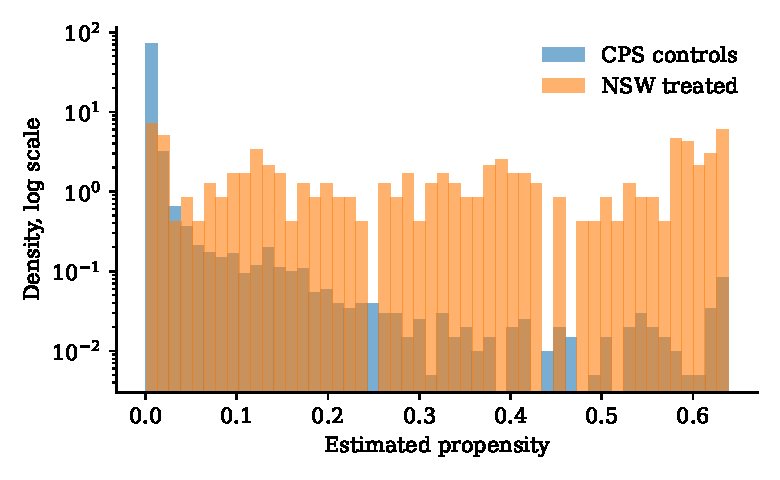
\includegraphics[width=\linewidth]{lalonde_ps.pdf}
\caption{Estimated propensity of NSW treatment among NSW treated and CPS controls, log density scale.}
\label{fig:lalonde_ps}
\end{figure}

\subsection{Results}

We estimate the effect on the treated, the natural target since the experimental benchmark concerns NSW participants. Table~\ref{tab:lalonde} and Figure~\ref{fig:lalonde_att} collect the estimates\index{LaLonde benchmark!results|textbf}. Hill's (2011) BART takes treatment as one more covariate and imputes each treated participant's control earnings; the next BART row adds the estimated propensity as a covariate, and the Bayesian causal forest takes it as an input. Every adjusted row uses the ten covariates. The propensity of Figure~\ref{fig:lalonde_ps}, which BART and the causal forest use, is a logistic regression on them; DML fits random forests for both the control outcome and its own propensity, with five folds and one random partition. The BART and causal forest\index{causal forest} posteriors keep 1,000 draws.

\begin{table}[ht]
\centering
\caption{Effect of NSW training on 1978 earnings of the treated, thousands of dollars, using CPS controls. Intervals are 95\% confidence intervals for least squares (heteroskedasticity robust) and DML, and posterior intervals otherwise. The experimental benchmark is 1.79. The BART rows average observed minus imputed earnings over the treated, so their intervals hold the treated outcomes fixed; the DML and causal forest intervals do not.}
\label{tab:lalonde}
\small
\begin{tabular}{p{2.5in}cc}
\toprule
Method & Estimate & Interval \\
\midrule
Difference in means & $-8.50$ & \\
Least squares & 1.07 & [$-0.16$, 2.29] \\
DML, augmented weighting for the treated, forests & 1.51 & [0.07, 2.95] \\
Hill's BART & 1.54 & [0.85, 2.16] \\
BART with estimated propensity & 1.51 & [0.77, 2.28] \\
BART after common support check & 1.39 & [0.70, 2.03] \\
Bayesian causal forest & 1.68 & [0.41, 2.88] \\
\bottomrule
\end{tabular}
\end{table}

\begin{figure}[ht]
\centering
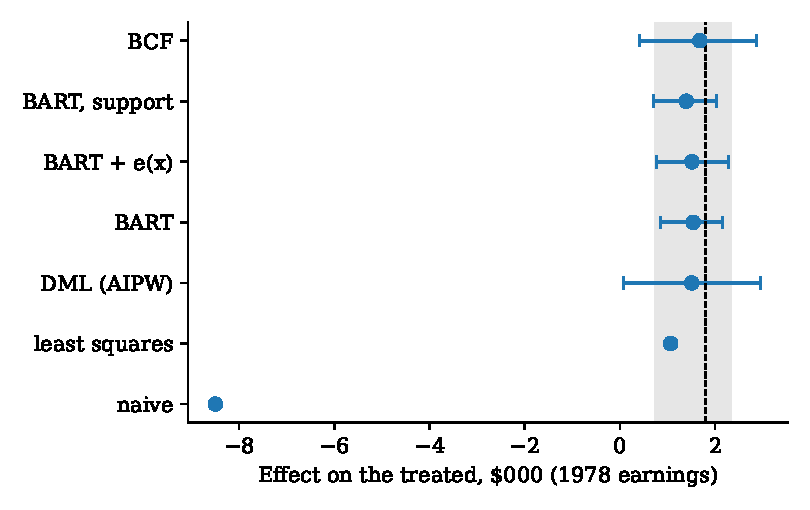
\includegraphics[width=\linewidth]{lalonde_att.pdf}
\caption{Estimates of the effect on the treated with CPS controls. The shaded band is the 95\% posterior interval from BART on the experimental data; the dashed line is the experimental difference in means.}
\label{fig:lalonde_att}
\end{figure}

Every flexible method lands within the experimental posterior band, and so does least squares at 1.07, so on these 185 treated participants the band does not tell the methods apart.  The tree based estimates move with the random seed and the machine: four independent chains of 2,000 draws gave means of 1.52 to 1.65 for BART with the estimated propensity and 1.68 to 1.74 for the causal forest, so differences of a tenth or two among the rows carry no information. The chains agree (split $\hat R$ at most 1.017), but the effective sample size of the effect for BART with the propensity is only 124 of the 8,000 draws. The common support\index{overlap} check (Chapter~\ref{ch:bart}) drops treated participants whose imputed control outcome has posterior standard deviation above the 99th percentile of the controls' standard deviations. It flagged 6 of the 185 treated as having poorly predicted counterfactuals, and the effect for the remaining 179 is 1.39.

The intervals differ more than the point estimates. Hill's BART is tightest, about 1.3 thousand dollars wide; DML's is widest, nearly 2.9. Most of the gap is a difference of estimand. The BART rows average observed minus imputed earnings over the 185 treated, so their posteriors hold the treated participants' earnings fixed and carry only the uncertainty about the mean control earnings at their covariates, not the variation of individual earnings around that mean. The DML interval is for the population effect on the treated and includes the sampling variability of their earnings. The treated term of its score alone has standard error 0.62, which already gives an interval wider than any BART row, and the reweighted controls have a standard error of 0.39; the two parts together give the reported 0.73. Those controls enter with the odds $e/(1 - e)$, which reached 8 for the most treated like controls. The experiment shows the same gap: the experimental difference in means\index{difference in means} has standard error 0.67, a half width of 1.32, while the BART interval from the same data has half width 0.79. The Bayesian causal forest is nearly as wide as DML. It averages draws of the effect function $\tau(x)$ over the treated, so its posterior carries uncertainty about the treated participants' mean earnings as well as their control earnings, where the BART rows use the observed earnings instead. Putting the BART rows on the causal forest's target, by averaging each draw of $\tau(x)$ over the treated, moves no point estimate by more than 0.19 and widens the intervals: Hill's BART gives 1.54 [0.41, 2.63], BART with the propensity 1.49 [0.27, 2.69] and the support checked fit 1.57 [0.44, 2.65], each about 2.2 to 2.4 thousand dollars wide, and the experimental BART interval widens from 1.58 to 2.32 around 1.37. That closes 58 percent of the width gap between Hill's BART and DML. We have not split the remaining 0.66 thousand dollars into comparable parts; BART already carries uncertainty about the control means, so the DML control term does not account for it by itself.

\paragraph{Conditional effects.} Figure~\ref{fig:lalonde_cate} plots the Bayesian causal forest's posterior for the conditional average effect $\tau(x)$ at each treated participant's covariates. These are effects for people like each participant, not the participant's own difference $Y_i(1) - Y_i(0)$, whose distribution depends on the joint law of the potential outcomes (Chapter~\ref{ch:gente}). The intervals are wide, as they must be with 185 treated units, and most overlap zero. There is little evidence of strong heterogeneity in 1975 earnings, though this is weak evidence of homogeneity: the prior holds the effect forest near a constant and the data have not pulled it far.

\begin{figure}[ht]
\centering
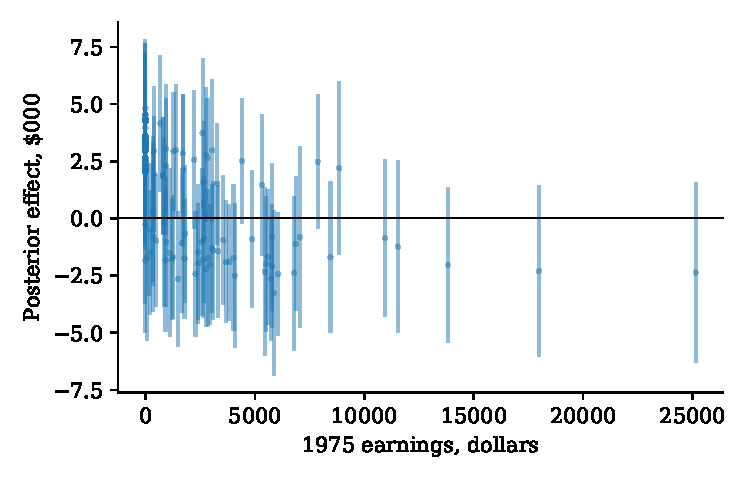
\includegraphics[width=\linewidth]{lalonde_cate.pdf}
\caption{Bayesian causal forest posterior of the conditional average effect at each NSW participant's covariates, against 1975 earnings: posterior means with approximate 95\% intervals (plus or minus 1.96 posterior standard deviations).}
\label{fig:lalonde_cate}
\end{figure}

\paragraph{Sensitivity to unmeasured confounding.} Figure~\ref{fig:lalonde_sens} applies the Bayesian sensitivity analysis\index{sensitivity analysis} of Section~\ref{sec:sensitivity} to the BART\index{Bayesian additive regression trees} posterior for the effect on the treated. That posterior has mean 1.54 and standard deviation 0.33 thousand dollars, and it holds the treated outcomes fixed, as the caption of Table~\ref{tab:lalonde} says. We approximate it by a normal distribution with those two moments and subtract the bias $a\,b_U$ of the linear example of that section: $a$ is the difference between trainees and controls, given the ten covariates, in an unmeasured confounder $U$ of unit variance, and $b_U$ is the change in 1978 earnings, in thousands of dollars, per standard deviation of $U$. Both get independent $N(0, s^2)$ priors, and the curve gives the probability of a positive effect at 60 values of $s$ from 0.01 to 1.5, each from 200,000 Monte Carlo draws. Near $s = 0.5$ the posterior probability of a positive effect is still 0.999; near $s = 1$ it is 0.94; at $s = 1.5$, 0.84. Because both priors are centred at zero, the bias is as likely to raise the estimate as to lower it, so the posterior mean stays at 1.54 and only the spread grows. Even a prior allowing confounding comparable to the full effect leaves that probability at 0.84.

\begin{figure}[ht]
\centering
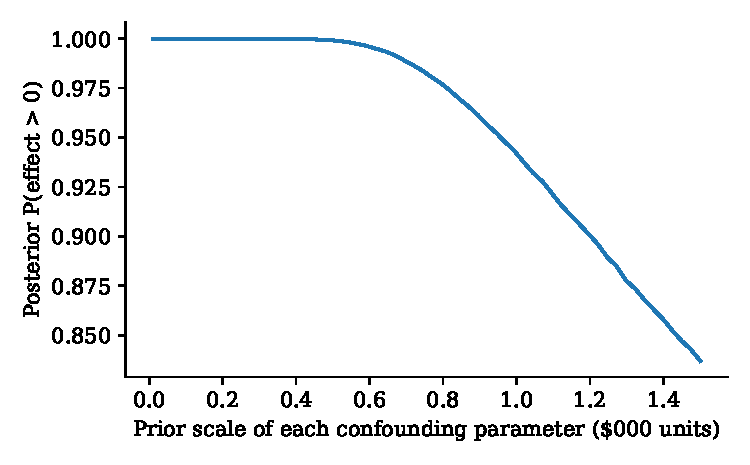
\includegraphics[width=\linewidth]{lalonde_sens.pdf}
\caption{Posterior probability that the NSW programme raised earnings, against the common prior scale $s$ of the two confounding parameters $a$ and $b_U$ of Section~\ref{sec:sensitivity}, starting from a normal approximation to the BART posterior for the effect on the treated (200,000 Monte Carlo draws at each of 60 values of $s$).}
\label{fig:lalonde_sens}
\end{figure}

\subsection{What the benchmark shows}

With 185 treated participants, this sample does not separate rigid from flexible adjustment\index{LaLonde benchmark!what it shows|textbf}. Least squares with linear covariates gives 1.07, with standard error 0.63, and the flexible methods give 1.39 to 1.68. The flexible estimates are closer to the experimental 1.79 and to the BART estimate from the experimental data, 1.55, but gaps of 0.3 to 0.6, about one standard error, cannot say that they are better. LaLonde's original estimates, built on similar parametric specifications, scattered widely, and earlier in this chapter the move from nine covariates to the 54 term basis changed least squares from 5.90 to 9.84, a change that no benchmark checks but that every flexible method shares.

Flexible adjustment lands near the experimental benchmark on this sample, whether through trees in a Bayesian model or forests inside DML, consistent with Dehejia and Wahba's conclusion and subject to Smith and Todd's warning that the subsample matters. We have not repeated the analysis on LaLonde's harder full sample, and readers should not generalize beyond these data.

\section{In practice}

\paragraph{The target.} In the 401(k) analysis the targets are the average effect, the effects on the treated and untreated, and the effect by income quintile. Each Gibbs draw of the coupled horseshoe model gives the five quintile effects, and weighting them by quintile shares in the chosen population gives a draw of each average, so the accountings and their intervals come from one set of draws. In the LaLonde analysis the target is the effect on the treated: each posterior draw of the response surface imputes each treated participant's control earnings, and averaging observed minus imputed earnings over them gives a draw of the target. Restricting the average to participants with common support, or any subgroup, is another accounting of the same draws.

\paragraph{What the analyst does differently.} The analyst states the population before fitting: a policymaker extending eligibility needs the effect on the untreated, 6.86, not the effect on the treated, 11.65. She expands the nine covariates to the 54 term basis, places the horseshoe on it with the propensity coupled into the prior, and fits a second model class, here the Bayesian causal forest; because its chains do not mix, she reports no estimates from it and says that the check remains to be done. She runs the predictive check of Figure~\ref{fig:ppc401k}, finds the Gaussian error model too symmetric, refits with Student $t$ errors, and reports the mean effect from the Gaussian working model and the shift of the bulk from the $t$ fit, labelled as different quantities. She reports Table~\ref{tab:k401q} and the three accountings together, because the decision depends on them. In the LaLonde analysis she looks at the propensity of Figure~\ref{fig:lalonde_ps} before fitting anything, which shows that most of the CPS sample is irrelevant. She checks common support unit by unit and reports the effect for all 185 treated (1.54) and for the 179 with support (1.39), and she presents the sensitivity of the sign to unmeasured confounding as the curve of Figure~\ref{fig:lalonde_sens}.

\paragraph{Against DML.} On the single weighted average that the partially linear DML score and the constant effect horseshoe both estimate, DML is adequate: 8.59 with forests and 9.52 with the lasso, intervals about 5 thousand dollars wide, against 9.82 and an interval of the same width from the horseshoe. Nothing in Table~\ref{tab:k401} separates the two on that question. Beyond that one number the lasso estimate moves from 9.52 to 10.26 across random partitions, each new accounting needs a new score, and DML recovers the quintile effects that turned out to be the finding of the 401(k) analysis, with an interval much wider than the posterior's in the top quintile. Stacking the five scores gives joint inference and intervals for differences between quintiles (Chernozhukov et al. 2018); what DML does not give is a probability for a statement such as the effect rising from each quintile to the next. On the LaLonde sample DML is adequate in the same way: 1.51 with forests and the augmented score, against 1.54 for Hill's BART and 1.68 for the Bayesian causal forest, inside the experimental band. It has no counterpart to the conditional effect posteriors of Figure~\ref{fig:lalonde_cate} or to the unit level check that found 6 treated participants without support.

\section*{Notes}

The 401(k) data are Chernozhukov and Hansen's (2004) extract of the 1991 Survey of Income and Program Participation. Regularization induced confounding is from Hahn, Carvalho, Puelz and He (2018). The $e(x)\{1 - e(x)\}$ weights are Li, Morgan and Zaslavsky's (2018) overlap weights (Chapter~\ref{ch:ipw}), and that a regression coefficient estimates a weighted average of this form is classical (Angrist 1998; Aronow and Samii 2016).

BART as a causal method is Hill's (2011), the Bayesian causal forest is Hahn, Murray and Carvalho's (2020), and the common support rule is Hill and Su's (2013); Chapter~\ref{ch:bart} describes all three.



\begin{exercises}
\item\label{ex:chk401:1} Derive the Gibbs step for the weights $w_i$ of the Student $t$ refit in Section~\ref{sec:k401overlap}, and explain why the common effect falls as the degrees of freedom fall.
\item\label{ex:chk401:2} Replace the income quintile interactions with a horseshoe on interactions of eligibility with every basis term, and report the posterior of $\tau(x)$ along a grid of incomes.
\item\label{ex:chk401:3} Compute the DML estimate of the effect on the treated using the appropriate orthogonal score, and compare it with the accounting value 11.65.
\item\label{ex:chk401:4} Using the propensity estimates, trim households with propensity below 0.05 and recompute the effect for the trimmed population, both by DML and as an accounting of the posterior.
\item\label{ex:chk401:5} Discuss whether the Poterba, Venti and Wise argument for unconfoundedness is credible, and design a Bayesian sensitivity analysis for an unmeasured taste for saving.

\item\label{ex:chlalonde:1} Repeat the analysis of Section~\ref{sec:lalonde} with LaLonde's PSID comparison group, which Dehejia distributes with the Dehejia and Wahba samples and which is in the book's data folder, and compare the spread of estimates with Table~\ref{tab:lalonde}.
\item\label{ex:chlalonde:2} Fit the coupled horseshoe of Chapter~\ref{ch:horseshoe} with a spline basis in 1974 and 1975 earnings, and compare with the BART estimates.
\item\label{ex:chlalonde:3} With $\mu_0(x) = \E(Y \mid T = 0, X = x)$ and $\tau_T$ the effect on the treated, the augmented score for $\tau_T$ is $\psi = \{T(Y - \mu_0(X) - \tau_T) - (1 - T)\,e(X)\{Y - \mu_0(X)\}/(1 - e(X))\}/\Prob(T = 1)$. Show that controls enter with weight $e(x)/\{1 - e(x)\}$, the weight that removes the error of $\mu_0$ on the treated, and explain why this places heavy weight on the few CPS controls that resemble the trainees.
\item\label{ex:chlalonde:4} Using the posterior draws, compute the posterior probability that the effect on the treated exceeds one thousand dollars under each Bayesian method.
\item\label{ex:chlalonde:5} Smith and Todd argue that matching estimates on these data are sensitive to the subsample. Design a Bayesian analysis that makes the dependence on the subsample explicit.
\end{exercises}

\chapter{Two Applications in Health}\label{ch:nhefs}

\begin{tcolorbox}[colback=gray!6,colframe=gray!50,title=In brief,fonttitle=\normalfont\itshape,coltitle=black,colbacktitle=gray!15,boxrule=0.4pt,arc=1pt]
Quitting smoking causes about three and a half kilograms of extra weight gain over eleven years. Three different Bayesian models agree with each other and with Hern\'an and Robins, and the causal forest shows little heterogeneity by smoking intensity or age. In Thornton's randomized HIV trial, one logistic model gives a risk difference of 0.447 for any incentive and conditional and marginal odds ratios of 7.46 and 7.23, and the dose response jumps from 0.34 to about 0.62 at the smallest incentive.
\end{tcolorbox}

This chapter returns to smoking from the other side. Many smokers fear that quitting will make them gain weight, a real barrier to quitting. We ask how much weight quitting causes. The question is observational, since no one can randomize cessation, and we compare our estimates with those of Hern\'an and Robins's \emph{Causal Inference: What If}. Section~\ref{sec:thornton} applies the same accounting to a randomized trial, Thornton's HIV incentives experiment.

\section{The data}

The National Health and Nutrition Examination Survey Epidemiologic Followup Study, NHEFS\index{NHEFS|textbf}, measured American adults in 1971 and again in 1982. We use the 1,566 smokers in 1971 with complete data, 403 of whom had quit by 1982. The outcome is the change in body weight\index{NHEFS!weight change after quitting smoking|textbf}, in kilograms, between 1971 and 1982. Following Hern\'an and Robins, the confounders are sex, race, age, education, cigarettes per day, years of smoking, exercise, usual daily activity, and 1971 weight, with squares of the four continuous variables.

The treatment is quitting at some time between the two surveys, a mixture of quit dates and later smoking histories, not eleven years without a cigarette, and the consistency assumption of Chapter~\ref{ch:predictive} is read with that version of treatment. The 63 smokers in the Hern\'an and Robins file with no 1982 weight are left out, so every estimate assumes that, given treatment and the covariates, whether a weight was recorded is unrelated to weight change; Hern\'an and Robins (2020) reweight for this censoring instead.

Quitters differed in education and activity. On average quitters were 46.2 years old (nonquitters 42.8), smoked 18.6 cigarettes a day (21.2) for 26.0 years (24.1), and weighed 72.4 kilograms in 1971 (70.3). Their raw weight change was 4.5 kilograms, against 2.0 for nonquitters. Older people gain less weight, and lighter smokers gain differently from heavy ones, so a raw comparison is not causal.

A smoker resolved to quit may also be resolved to eat less or exercise more, and that resolve is not in the 1971 covariates. We assume, as Hern\'an and Robins do and as the price of comparing methods on a common footing, that the nine covariates capture everything that drives both quitting and weight change; the squares of the four continuous ones belong to the regression, not to the assumption. Overlap\index{overlap} is good. In the Hern\'an and Robins logistic model the estimated propensities run from 0.05 to 0.78, the largest stabilized weight is 4.3, and the effective sample size of the weights is 1,446 of 1,566. With no thin tail of the kind that dominated the LaLonde benchmark of Section~\ref{sec:lalonde}, weighting and outcome modelling should agree, and the comparison isolates the error model and the prior rather than the handling of extreme weights.

\section{Results}

Table~\ref{tab:nhefs} and Figure~\ref{fig:nhefsate} report the estimated average effect of quitting on eleven year weight change\index{NHEFS!results|textbf}.

\begin{table}[ht]
\centering
\caption{Effect of quitting smoking on weight gain from 1971 to 1982, kilograms. Intervals are 95\% confidence intervals for least squares and DML and 95\% posterior intervals for the Bayesian methods.}
\label{tab:nhefs}
\small
\begin{tabular}{p{2.5in}cc}
\toprule
Method & Estimate & Interval \\
\midrule
Difference in means & 2.54 & \\
Least squares, Hern\'an and Robins covariates & 3.46 & [2.60, 4.32] \\
Inverse probability weighting, stabilized & 3.44 & \\
DML, augmented weighting, forests & 3.71 & [2.59, 4.84] \\
Horseshoe, coupled, with effect modifiers & 3.48 & [2.60, 4.34] \\
BART, Hill's approach & 3.23 & [2.37, 4.09] \\
Bayesian causal forest & 3.41 & [2.58, 4.28] \\
\bottomrule
\end{tabular}
\end{table}

\begin{figure}[ht]
\centering
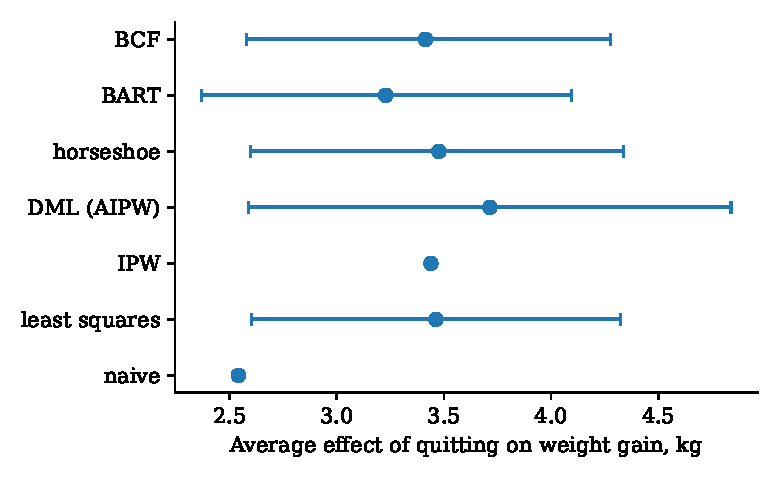
\includegraphics[width=\linewidth]{nhefs_ate.pdf}
\caption{Estimates and 95\% intervals of Table~\ref{tab:nhefs} for the average effect of quitting smoking on eleven year weight gain.}
\label{fig:nhefsate}
\end{figure}

Adjustment raises the estimate from 2.5 to about 3.4 kilograms. Our inverse weighting estimate of 3.44 reproduces the value of about 3.4 reported by Hern\'an and Robins, which confirms that we use the same data and confounders. Our least squares row enters their covariates additively and gives 3.46; their standardization estimate of about 3.5 also lets the effect of quitting vary with cigarettes per day and averages over all 1,629 smokers in their file, including the 63 with no 1982 weight. 

The horseshoe row of Table~\ref{tab:nhefs} uses the standardized Hern\'an and Robins basis (the four continuous covariates, their squares, and dummies for sex, race, education, exercise and activity) plus the effect modifiers, interactions of treatment with the four continuous covariates. Coupled means that treatment, the intercept and the estimated propensity are unpenalized (Chapter~\ref{ch:horseshoe}); the sampler runs 3,000 Gibbs iterations, 1,000 of them burn-in. BART takes treatment as a covariate and the causal forest uses the logistic propensity, both on the nine raw covariates with 20 warm-start sweeps and 1,000 MCMC draws. DML is the augmented score with five-fold cross fitting, forests of 500 trees (minimum leaf 5) for each arm's outcome and the propensity, propensities clipped to $[0.01, 0.99]$, and a normal interval from the score's standard deviation.

\section{Heterogeneity}

Does the effect of quitting grow with smoking intensity\index{NHEFS!heterogeneity|textbf}? Figure~\ref{fig:nhefshet} shows the Bayesian causal forest\index{Bayesian causal forest}'s posterior averaged within four groups of 1971 cigarettes per day, 1 to 10, 11 to 19, exactly 20 and 21 or more (406, 155, 563 and 442 smokers; more than a third report exactly 20, so equal fifths cannot be cut), and within quintiles of age. The effect rises slightly with intensity\index{heterogeneous treatment effects!by smoking intensity|textbf}, from about 3.1 kilograms among the lightest smokers to about 3.6 among the heaviest, but the intervals overlap heavily. With age the pattern is an inverted U, smallest in the oldest quintile (ages 56 to 74) at about 2.9 kilograms, interval 1.3 to 4.1.

\begin{figure}[ht]
\centering
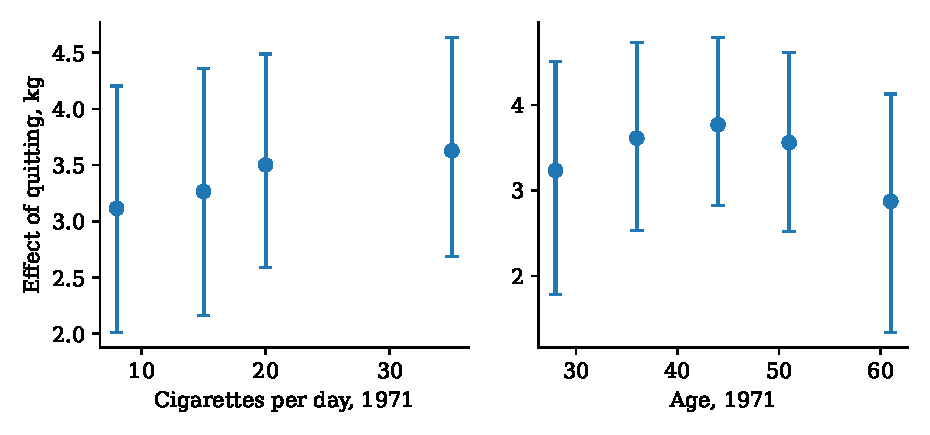
\includegraphics[width=\linewidth]{nhefs_het.pdf}
\caption{Bayesian causal forest posterior of the effect of quitting on weight gain, averaged within four groups of 1971 cigarettes per day (left) and quintiles of age (right), plotted at the group medians, with 95\% intervals.}
\label{fig:nhefshet}
\end{figure}

Under the causal forest, the effect on quitters is 3.36 kilograms, interval 2.56 to 4.21, and on nonquitters 3.43, interval 2.58 to 4.32. With modest heterogeneity, the choice of population matters little.

\section{What the comparison shows}

Every adjusted method agrees within about half a kilogram, well inside any interval. As in the LaLonde benchmark (Section~\ref{sec:lalonde}), Bayesian intervals are narrower than DML's: about 1.7 kilograms wide against 2.3. Least squares, also about 1.7 kilograms wide, shows that the gap is not a property of Bayes as such. It comes from fitting an outcome model, which pools across neighbouring covariate values and assumes a form for the regression, while the augmented score does not trust its outcome forests and adds back each residual divided by an estimated propensity. A narrower interval bought with a modelling assumption is worth having only if it keeps its coverage, which the widths alone cannot show.

A simulation built on these data checks the coverage. It keeps the 1,566 covariate vectors, draws treatment from the fitted logistic propensities, takes the mean without quitting from the additive least squares fit, and adds an effect that is either constant at 3.5 kilograms or 3.5 plus a centred and scaled function of age and cigarettes per day ($\sin z_{\mathrm{age}} + z_{\mathrm{cig}}^2$ in standardized units, so its standard deviation is 1 kilogram); the sample average effect is 3.5 in every design. The errors have standard deviation 7.3 kilograms, close to the residual standard deviation of the fits, and are either Gaussian or Student $t$ on four degrees of freedom divided by $\sqrt{2}$, which has the same standard deviation. Each of the four designs has 500 replications, and least squares, DML, the horseshoe, BART and the causal forest are refitted to every replicate with the settings above, propensities included.

Table~\ref{tab:nhefssim} gives the results. Least squares, the horseshoe and the causal forest cover between 93.8 and 96.2 percent with intervals 1.72 to 1.74 kilograms wide, against a Monte Carlo standard error of about one point. DML covers 93.4 to 98.0 percent with intervals of 2.07 to 2.10 kilograms, and its root mean squared error is 10 to 20 percent larger. BART, with treatment as a covariate, shrinks the effect by 0.15 to 0.25 kilograms and covers 91.4 percent when the effect is constant, which matches its lower estimate in Table~\ref{tab:nhefs}.

The design is kinder than the data. A posterior predictive check of the horseshoe and the causal forest, with one replicated data set from each posterior draw at the draw's error variance, finds weight change more peaked among nonquitters, and with a longer right tail in both groups, than Gaussian errors allow: the largest observed changes are 47.5 and 48.5 kilograms, against replicated maxima near 27. Weight change is also more spread out among quitters (standard deviation 8.7, against 7.9 replicated by the horseshoe) than among nonquitters (7.4 against 7.8), while the simulated errors have one variance for everyone.

\begin{table}[ht]
\centering
\caption{Simulation on the NHEFS covariates, 500 replications per design, true average effect 3.5 kilograms: coverage of nominal 95\% intervals (Monte Carlo standard error 0.006 to 0.013), the range of the bias over the four designs, and the mean interval width averaged over them, in kilograms.}
\label{tab:nhefssim}
\footnotesize
\setlength{\tabcolsep}{4pt}
\begin{tabular}{lcccccc}
\toprule
 & & \multicolumn{2}{c}{Constant effect} & \multicolumn{2}{c}{Varying effect} & \\
Method & Bias & Gaussian & $t_4$ & Gaussian & $t_4$ & Width \\
\midrule
Least squares & 0.00 to 0.10 & 0.940 & 0.952 & 0.962 & 0.946 & 1.73 \\
DML & $-0.03$ to 0.02 & 0.934 & 0.972 & 0.980 & 0.960 & 2.08 \\
Horseshoe & 0.00 to 0.09 & 0.940 & 0.954 & 0.960 & 0.946 & 1.74 \\
BART & $-0.25$ to $-0.15$ & 0.914 & 0.914 & 0.946 & 0.942 & 1.70 \\
Bayesian causal forest & $-0.10$ to $-0.01$ & 0.938 & 0.940 & 0.960 & 0.956 & 1.74 \\
\bottomrule
\end{tabular}
\end{table}

The three Bayesian models, a fixed basis and two kinds of trees, agree within about a quarter of a kilogram. Functional form does not drive the number.

All of this assumes that the measured covariates remove the confounding. The Bayesian form of the sensitivity analysis of Section~\ref{sec:sensitivity} carries over to a continuous outcome. Suppose an unmeasured confounder $U$ of unit variance adds $b$ kilograms of weight change per standard deviation, for quitters and nonquitters alike, and that its mean among quitters exceeds its mean among nonquitters by $a$ at every value of the measured covariates. Quitters and nonquitters with covariates $x$ then differ in expected weight change by $\tau(x) + ab$, so every estimate of the average effect is biased by $ab$, and each posterior draw is corrected by subtracting it.

The data cannot update $a$ and $b$, so their priors are scaled by the strongest measured confounder. For each covariate we standardize its part of the least squares fit, its linear and squared terms together: $b$ is the standard deviation of that part in kilograms and $a$ the coefficient of quitting in its regression on quitting and the other covariates. Age has the largest product, $b = 2.47$ and $a = -0.10$, ahead of 1971 weight. With independent priors $a \sim N(0, m^2 a_{\mathrm{age}}^2)$ and $b \sim N(0, m^2 b_{\mathrm{age}}^2)$, a confounder $m$ times as strong as age on both links, each of 2,000 horseshoe draws and 1,000 causal forest draws of the effect is paired with 100 prior draws. Figure~\ref{fig:nhefssens} shows the posterior probability that the effect exceeds 0 and 1 kilogram. A prior centred at zero only widens the posterior: at $m = 1$ the horseshoe interval goes from 2.60 to 4.34 to 2.48 to 4.48, at $m = 2$ to 1.16 to 5.81 with probability 0.99 that the effect is positive, and at $m = 4$ that probability is 0.87. The right panel gives $a$ and $b$ the same scales but signs that inflate the estimate: the probability of a positive effect is still 0.99 at $m = 2$, with posterior mean 2.83 kilograms, and falls to 0.75 at $m = 4$, with mean 0.89. The causal forest gives nearly the same curves. The conclusion that quitting adds weight survives a hidden confounder twice as strong as age on both links; one four times as strong makes the sign uncertain.

\begin{figure}[ht]
\centering
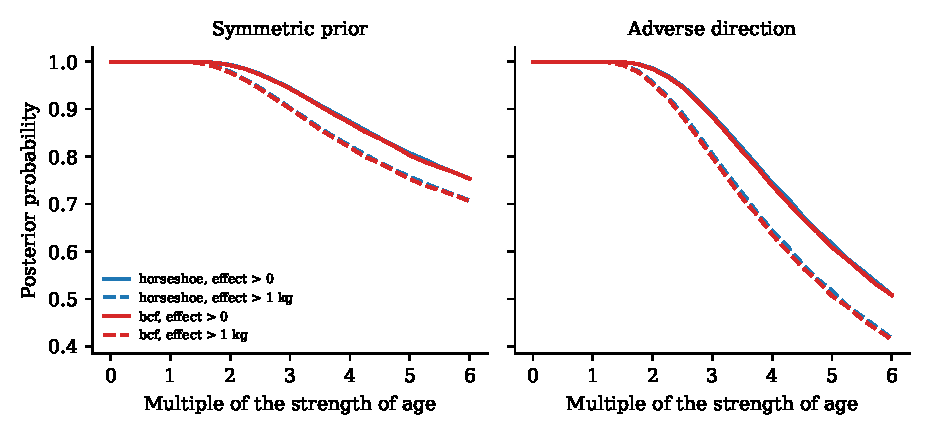
\includegraphics[width=\linewidth]{nhefs_sens.pdf}
\caption{Posterior probability that the effect of quitting exceeds 0 kilograms (solid) and 1 kilogram (dashed) when an unmeasured confounder is $m$ times as strong as age on both links, for the horseshoe and the Bayesian causal forest, whose curves nearly coincide. Left: normal priors centred at zero on the two links. Right: the same scales with the signs that inflate the estimate.}
\label{fig:nhefssens}
\end{figure}

A smoker asking how much weight quitting will likely add gets a posterior predictive answer for her age, sex and smoking history, from the horseshoe with effect modifiers of Table~\ref{tab:nhefs}. Her expected extra gain, the difference between her predictive means under quitting and under not quitting, is close to the average of about three and a half kilograms over eleven years, small against the very large risk reductions of Chapter~\ref{ch:smoking}. The two predictive distributions are far wider than that difference, because weight change varies a great deal between people with the same covariates, so they overlap heavily, and their right tails are too light, as the predictive check above found. Exercise~\ref{ex:chnhefs:4} asks for both, with a draw of the residual error at each draw's variance. The mean of her own gain from quitting is identified. Its spread is not, since it depends on the correlation between her two potential weight changes (Chapter~\ref{ch:gente}).

\section[Incentives and learning HIV status]{Incentives and learning HIV status: accounting in a randomized trial}\label{sec:thornton}

Rebecca Thornton's (2008) experiment\index{Thornton HIV incentive experiment|textbf} in rural Malawi asked whether small cash incentives would persuade people tested for HIV to return and learn their results. Incentives were assigned by lottery, so confounding is a small issue here, though the share offered an incentive differed by village, which the village intercepts below take into account. We use the experiment to show the model first argument on real data with a binary outcome: two logistic posteriors, one for any incentive and one for the amount, with every reported effect an accounting of one of them.

A randomized trial is the setting where the case for a model seems weakest. When every unit has the same chance of treatment, the difference in proportions is unbiased and a confidence interval for it needs no model at all. The reason to fit one anyway is that the questions asked of a trial are rarely limited to the single difference. Thornton randomized not only whether an incentive was offered but how much, and respondents lived at different distances from the centres, so the natural questions are whether the effect depends on distance, how the response rises with the amount, and how a risk difference relates to the odds ratios that the epidemiological literature reports.

\paragraph{The experiment.} Household survey respondents were offered free HIV tests at home. Each then received a voucher of randomly assigned value, possibly zero, redeemable on returning to a nearby centre to learn the result. The amounts take 27 distinct values, from 0 to 2.84 as coded in the data, and 21.9\% of respondents received none. Centres lay at varying distances from respondents' homes. The outcome is whether the respondent learned the result. We use the 2,816 respondents with a valid test result and complete data on outcome, incentive, distance and age.

Of those who received any incentive, 78.9\% learned their result; of those who received none, 34.1\%. The incentive more than doubled the rate.

\subsection{One logistic posterior}

We fit the logistic model
\begin{multline*}
\logit\Prob(\text{learned} = 1) = \alpha + \tau\,\mathrm{any} + \beta_1\,\mathrm{dist} \\
+ \beta_2\,\mathrm{age} + \delta\,\mathrm{any}\times\mathrm{dist},
\end{multline*}
with distance and age standardized and independent normal priors of variance 10 on the coefficients, by Polya Gamma\index{Polya Gamma@P\'olya Gamma} Gibbs sampling (Chapter~\ref{ch:computation}). We retain 2,000 posterior\index{Thornton HIV incentive experiment!one logistic posterior|textbf} draws.

\begin{table}[ht]
\centering
\caption{Accountings of one logistic posterior for the Thornton experiment.}
\label{tab:thornton}
\small
\begin{tabular}{p{2.1in}cc}
\toprule
Summary & Posterior mean & 95\% interval \\
\midrule
Risk difference, sample average & 0.447 & [0.404, 0.486] \\
Risk difference, nearest quarter by distance & 0.422 & [0.358, 0.486] \\
Risk difference, farthest quarter by distance & 0.472 & [0.399, 0.540] \\
Conditional odds ratio, at mean distance & 7.46 & [6.09, 9.08] \\
Marginal odds ratio, sample & 7.23 & [5.90, 8.75] \\
\bottomrule
\end{tabular}
\end{table}

The sample risk difference\index{risk difference|textbf} is 0.447: any incentive raised the probability of learning one's status by about 45 percentage points. The effect is somewhat larger for those farthest from the centre, 0.47, than for those nearest, 0.42, though the two intervals overlap.

The lottery did not give every village the same odds. Among the 119 villages (2 to 127 respondents each, median 17) the share offered any incentive runs from none to all, and a chi squared test of equal shares gives 347 on 118 degrees of freedom, $p$ about $2 \times 10^{-24}$. The data file records the village but not Thornton's district, so as a robustness check we refit the model with a village intercept $u_j \sim N(0, \sigma^2)$, a half Cauchy prior with scale 1 on $\sigma$, and an intercept of its own for each of the four respondents with no village number; the dose model below gets the same intercepts. The Polya Gamma sampler draws the coefficients and the intercepts in one block, four chains of 4,000 iterations with 1,000 discarded. The village scale $\sigma$ is 0.60 on the logit scale (interval 0.43 to 0.80), and the sample risk difference, averaged over respondents with their own village effects, moves only from 0.447 to 0.438 (interval 0.40 to 0.48), with 0.41 for the nearest quarter and 0.46 for the farthest. Table~\ref{tab:thornton} and Figure~\ref{fig:thornton} report the model without village intercepts.

\subsection{Noncollapsibility in real data}

The conditional odds ratio\index{odds ratio!conditional and marginal|textbf}, $e^\tau$ at mean distance, is 7.46. At each draw, $p_{ti}$ is respondent $i$'s fitted probability of learning the result under $\mathrm{any} = t$ and $\bar p_t$ its sample average. The marginal odds ratio is
\[
\frac{\bar p_1/(1-\bar p_1)}{\bar p_0/(1-\bar p_0)},
\]
with posterior mean 7.23. They differ, and confounding plays no part in the gap: both are computed from the same fitted model over the same respondents. This is the noncollapsibility\index{noncollapsibility} of Chapter~\ref{ch:mccullagh} in real data\index{noncollapsibility!in real data|textbf}\index{Thornton HIV incentive experiment!noncollapsibility in real data|textbf}. The model also lets the effect vary with distance, so 7.46 is the conditional ratio at mean distance only, but the posterior puts that interaction near zero (mean 0.05, 95\% interval $-0.16$ to $0.26$), and the model without the interaction leaves almost the same gap, 0.21 against 0.23. In this model the difference is small because baseline risk varies only moderately with distance and age. Baseline risk also varies between villages, and with the village intercepts the conditional odds ratio, at mean distance in a typical village, rises to about 8.0 while the marginal one falls to 6.9, so the gap grows from 0.23 to about 1.1 (interval 0.6 to 1.7). Figure~\ref{fig:thornton} shows the two posteriors side by side.

Both numbers are correct; they answer different questions. An analyst reporting an odds ratio from a trial should say which one it is, and a reader comparing trials should expect the conditional ratio from a regression with covariates and the marginal ratio from a two by two table to differ even when both trials are perfectly randomized. The risk difference of 0.447 is collapsible, since $\bar p_1 - \bar p_0$ is the average of the respondents' own differences $p_{1i} - p_{0i}$, which is one reason to report it first. Exercise~\ref{ex:chthornton:1} asks when the two ratios coincide.

\begin{figure}[ht]
\centering
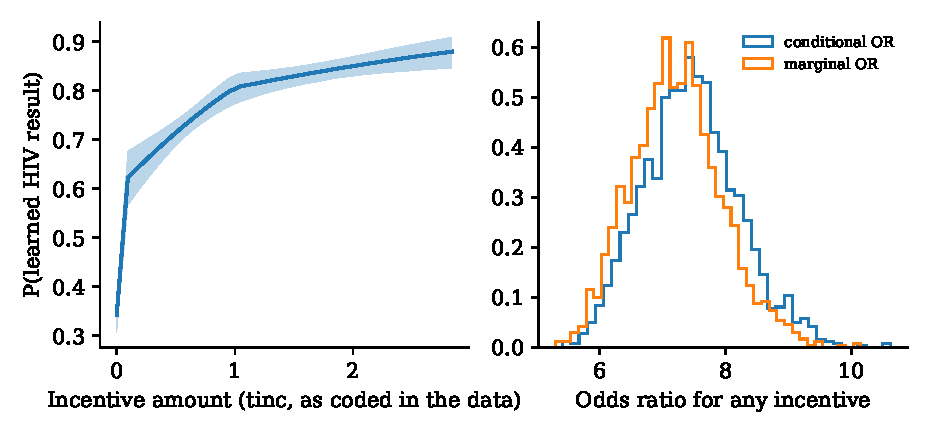
\includegraphics[width=\linewidth]{thornton.pdf}
\caption{Left: posterior mean and 95\% band of the probability of learning one's HIV result as a function of the incentive amount, from a logistic model with a jump at zero and a dose response piecewise linear on the logit scale, averaged over the sample. Right: posteriors of the conditional and marginal odds ratios for any incentive.}
\label{fig:thornton}
\end{figure}

\subsection{The dose response}

The incentive amount was also randomized, so the experiment identifies a dose response\index{Thornton HIV incentive experiment!dose response|textbf}\index{dose response|textbf}. A second logistic model, adjusting for distance and age, has an indicator for any incentive, the amount, and a change in slope at one unit of the amount as coded in the data. The left panel of Figure~\ref{fig:thornton} shows the result: the probability of learning one's result is 0.34 with no incentive and jumps to about 0.62 with the smallest positive incentive, then rises more slowly, to about 0.80 at one unit and 0.88 at the largest amount, 2.84. With the village intercepts the curve starts at 0.36 and reaches 0.60 at the smallest incentive, a jump of 0.24 rather than 0.28, and from one unit up the two curves differ by less than 0.003.

The shape matters for policy: most of the effect comes from offering any incentive at all, and larger amounts add less, as Thornton also concluded.

A programme with a fixed budget cares about the expected number of additional people who learn their status per unit spent. Write $p(a)$ for the probability of learning one's result at amount $a$, averaged over the sample. At a positive amount that number is $\{p(a) - p(0)\}/\{a\,p(a)\}$, the rise above the no incentive rate divided by the expected payout per person, the amount times the probability of collecting it. The jump at zero makes the smallest positive incentive by far the most cost effective, and the slower rise thereafter means that each additional unit buys less. Among the amounts offered, the smallest positive one wins in every posterior draw, with or without village intercepts, so the best amount for this ratio sits at the lower edge of the range tried, with posterior probability close to one. Below that edge the jump would keep raising the ratio, but no one was offered less, and the model has no data there.

A programme that values each additional person who learns her status at $V$ can instead maximize the net value $V\,[p(a) - p(0)] - a\,p(a)$ over the amount. The best amount has a posterior distribution that moves with $V$ (Exercise~\ref{ex:chthornton:3}). A programme that must commit to one amount takes the Bayes action of Chapter~\ref{ch:cdt}. The net value is linear in $p$, so this is the maximizer of $V\,[\bar p(a) - \bar p(0)] - a\,\bar p(a)$, with $\bar p$ the posterior mean curve of Figure~\ref{fig:thornton}, and it need not equal the mean or median of the posterior of the best amount. An analyst who reported only the average effect of any incentive, 0.447, would have told the policymaker that incentives work and nothing about how much to offer.

\section{In practice}

\paragraph{The target.} In the weight study each posterior draw of the causal forest gives $\tau(x_i)$ for every person, and averaging over all, over quitters, over nonquitters, or within a group of people gives a draw of each target. In the trial the targets are risk differences for chosen populations, conditional and marginal odds ratios, and the expected rate of learning under any incentive schedule, each a function of the logistic coefficients and covariates, evaluated at each posterior draw.

\paragraph{What the analyst does differently.} The analyst first reproduces the standard estimates, 3.44 by stabilized inverse weighting and 3.46 by least squares, to confirm the data before claiming anything new. She then fits at least two Bayesian models of different form, here three, and reports their agreement as evidence that functional form does not drive the answer. She reports the effect on quitters and on nonquitters, says explicitly that heterogeneity is modest, and answers the question a smoker actually asks, the predictive weight change for her own covariates. In the trial she reports the risk difference first, since it is collapsible, and then says which odds ratio she means. She also checks the assignment: the offer rate differs by village, so she refits with village intercepts and reports that the risk difference barely moves while the two odds ratios move apart. She shows the dose response with its posterior band.

\paragraph{Against DML.} DML with forests gives 3.71 with interval 2.59 to 4.84, compatible with every other adjusted row of Table~\ref{tab:nhefs}, and on the average effect it is adequate. The Bayesian case in the weight study rests on three things DML did not deliver. In this sample the interval was about 30 percent wider (2.25 kilograms against 1.74 for the horseshoe, 1.70 for the causal forest, and 1.72 for least squares, which also trusts its outcome model). The heterogeneity by intensity and age, and the effects on quitters and nonquitters, came from the fitted forest at no extra cost, as joint draws of one posterior. DML can reach the prespecified groups by averaging its score contributions within each group, and the effects on quitters and nonquitters by reweighting the same nuisance fits as in \eqref{eq:aipw:att}, but each is a separate estimate with its own interval. And the individual predictive answer has no DML analogue at all, because DML estimates a functional and not a model. In the trial a cross-fitted augmented estimator that knew the assignment probabilities would need no estimated propensity and would be unbiased for the risk difference whatever its outcome model. Here they differ by village and are not in the data file, so they would have to be estimated from the village offer rates, and the twelve villages in which everyone or no one was offered give no comparison. On that one number it is still adequate. The effect by distance, the two odds ratios and the dose response would each need a target and a score of their own, and the fitted logistic models give them from their posterior draws.

\section*{Notes}

Hern\'an and Robins (2020) use the NHEFS data to illustrate every classical method; they also treat the effect of quitting on mortality (Exercise~\ref{ex:chnhefs:3}) and time varying treatments (Section~\ref{fw:sec:gmethods}). The three Bayesian models are the horseshoe of Carvalho, Polson and Scott (2010) in the coupled form of Chapter~\ref{ch:horseshoe}, BART as a causal method from Hill (2011) and the Bayesian causal forest of Hahn, Murray and Carvalho (2020), the last two described in Chapter~\ref{ch:bart}. The DML comparison is the estimator of Chernozhukov and coauthors (2018).

Thornton (2008) also asks whether learning one's status changed later behaviour (Exercise~\ref{ex:chthornton:4}). The Polya Gamma sampler is from Polson, Scott and Windle (2013); see Chapter~\ref{ch:computation}. Greenland, Robins and Pearl (1999) discuss noncollapsibility, and Chapter~\ref{ch:mccullagh} gives the model first reading of it. Rubin (1978) is the place to read how randomization enters a Bayesian analysis of causal effects. Exercise~\ref{ex:chthornton:2} takes the village random effects further.


\begin{exercises}
\item\label{ex:chnhefs:1} Reproduce the Hern\'an and Robins inverse probability weighting estimate and its confidence interval, and compare with the posterior intervals in Table~\ref{tab:nhefs}.
\item\label{ex:chnhefs:2} Fit the coupled horseshoe without the effect modifier interactions and compare its posterior with the one reported here.
\item\label{ex:chnhefs:3} Hern\'an and Robins also analyse the effect of quitting on mortality. Fit a Bayesian survival model and report the posterior of the difference in ten year survival probability.
\item\label{ex:chnhefs:4} Using the horseshoe with effect modifiers, compute the posterior predictive distribution of weight change for a 45 year old woman who smoked 20 cigarettes a day for 25 years, with her other covariates at the sample medians, under quitting and not quitting.

\item\label{ex:chthornton:1} Show that the marginal and conditional odds ratios in Table~\ref{tab:thornton} would coincide if baseline risk did not vary with distance or age and $\delta = 0$.
\item\label{ex:chthornton:2} Refit the logistic model with village random effects, as in Section~\ref{sec:thornton}, and compare three risk differences: averaged over the respondents with their own village effects, over a new village drawn from the village distribution, and for a typical village with effect zero.
\item\label{ex:chthornton:3} Using the dose response model, let $p(a)$ be the probability of learning one's status at amount $a$, averaged over the sample, let $V$ be the value, in the units of the amount, of each additional person who learns her status, and take $a$ in the range of amounts offered. Find the amount that maximizes $V\,[p(a) - p(0)] - a\,p(a)$, the value net of the expected payout $a\,p(a)$, and report how its posterior distribution changes with $V$.
\item\label{ex:chthornton:4} Thornton also studied whether learning one's status changed later behaviour. Discuss what additional assumptions are needed to estimate that effect using the incentive as an instrument, in the framework of Chapter~\ref{ch:iv}.
\end{exercises}

\chapter{A Workflow for Applied Bayesian Causal Inference}\label{ch:workflow}

\begin{tcolorbox}[colback=gray!6,colframe=gray!50,title=In brief,fonttitle=\normalfont\itshape,coltitle=black,colbacktitle=gray!15,boxrule=0.4pt,arc=1pt]
The workflow has seven steps: state the question and the population, draw the assignment mechanism, check overlap, fit two flexible outcome models, check the model against the data, report accountings, and quantify sensitivity to unmeasured confounding. Steps~1 and~2 ask for the same statement and the same graph under any method; in Steps~3 to~7 the Bayesian analysis uses its posterior for more than an average. For one average effect, under the conditions set out at the end of the chapter, DML is enough.
\end{tcolorbox}

The 401(k), LaLonde, NHEFS and Thornton analyses of Chapters~\ref{ch:k401} and~\ref{ch:nhefs} share a sequence of seven steps\index{workflow!seven steps|textbf}. We set it out as a workflow\index{workflow|textbf} for the applied analyst, saying at each step what a DML analyst would do.

\section{Step 1: state the causal question and the population}

Before fitting any model, write down whom the decision concerns and what would be done differently\index{workflow!stating the causal question and the population|textbf}. In the 401(k) application the policy question was whether to extend eligibility to workers lacking it, making the effect on the untreated the relevant accounting. In LaLonde the benchmark concerned programme participants, so the effect on the treated\index{effect on the treated}. In the Thornton experiment the question was how large an incentive to offer, so the dose response was the target. For an observational study the statement is the protocol of the target trial it emulates (Section~\ref{fw:sec:obs}): eligibility, the treatment strategies and a start of follow up at which eligibility is met and treatment assigned, so that nothing measured after that start enters the adjustment set.

The population fixes the accounting: in the 401(k) data the effect on the untreated, 6.86 thousand dollars, was about 40\% below the 11.65 on the treated. For DML it also fixes the estimator: the effect on the treated needs a different orthogonal score from the average effect, and Chapter~\ref{ch:dml}'s partially linear score targets an overlap weighted average that need not equal the population average effect when effects vary. For the Bayesian analyst it fixes only the weights on the posterior draws, which can be changed without refitting.

\section{Step 2: draw the assignment mechanism}

Say how treatment was assigned, and draw the graph\index{assignment mechanism!drawing the|textbf}\index{workflow!drawing the assignment mechanism|textbf}: randomized, as in Thornton, though at offer rates that differ by village; determined by employers given observed worker characteristics, as argued for 401(k); or chosen by the person, as with quitting smoking. The LaLonde comparison sets National Supported Work (NSW) trainees recruited for disadvantage beside CPS survey controls; within the NSW itself assignment was random. Each mechanism suggests which covariates are confounders, which might be instruments, and where unmeasured confounding is most plausible. Section~\ref{sec:milk} showed the cost of skipping this step: the Lanarkshire\index{Lanarkshire milk experiment} teachers were a mechanism nobody modelled.

Mark every variable in the data as a pretreatment confounder, a mediator, a consequence of the outcome or an instrument, and write down unconfoundedness with the covariate set named. In the 401(k) data, record the Poterba, Venti and Wise argument: income and the other eight covariates are the confounders, and a taste for saving is the unmeasured variable most likely to break the assumption. In LaLonde, mark earnings history as the confounder separating the disadvantaged trainees from the CPS respondents who replace the randomized controls.

A DML analyst needs the same graph, and in practice receives a covariate list and treats it as the adjustment set. Orthogonalization protects her against nuisance estimation error, not against a wrong set: a mediator in the set biases DML as it biases any other method. For the Bayesian analyst the graph also determines the prior: whether to couple the outcome prior to the propensity depends on whether the covariates are confounders or instruments, and Step~7's sensitivity analysis is parametrized by the unmeasured variable the graph identified.

\section{Step 3: check overlap before modelling}

Fit a propensity model\index{propensity score}, not to weight by it but to see where the data are thin: plot both groups' estimated propensities on a log density scale (Figure~\ref{fig:lalonde_ps}), tabulate their quantiles, and record the region of covariate space where one group is absent\index{overlap!checking before modelling|textbf}\index{workflow!checking overlap|textbf}. Decide whether to restrict the target population to the region of overlap and say so in Step~1's statement. In LaLonde most CPS controls had propensities below one in a thousand and were irrelevant, and the odds $e/(1 - e)$ of DML's random forest propensity reached 8 for the most treated like controls. In the 401(k) data the thin region was low income (Section~\ref{sec:k401overlap}); in NHEFS overlap\index{overlap} was good. After fitting the outcome model, Hill's common support check gives a second, model based view, unit by unit.

DML estimates the propensity inside cross fitting. With an augmented score, thin overlap produces a few large weights that widen intervals or undermine the normal approximation. The usual remedy, trimming at a threshold such as 0.05, changes the target and must be reported.

The Bayesian outcome model pools across nearby covariate values instead of reweighting, so thin overlap becomes extrapolation. Posterior intervals may widen there, as in the bottom income quintile of Section~\ref{sec:k401overlap}, but a tree ensemble need not widen (Chapter~\ref{ch:bart}), so width alone is no guarantee. The common support check adds what no weight can: a unit by unit statement of which treated participants have counterfactuals with unusually large predictive uncertainty.

\section{Step 4: fit at least two flexible outcome models}

Fit two outcome model classes\index{workflow!fitting two flexible outcome models|textbf}, for example a coupled horseshoe\index{horseshoe prior} on a basis and a Bayesian causal forest\index{Bayesian causal forest}\index{Bayesian causal forest!in the workflow|textbf}. Unless Step~2 marked instruments among the covariates, include the estimated propensity as a covariate in both, fitted once on the whole sample without cross fitting (Section~\ref{sec:ricsim}), against regularization induced confounding\index{regularization induced confounding}. Where they agree, the conclusion does not depend on the choice between them, though both can share an extrapolation or a shrinkage bias that agreement cannot reveal. They agreed closely on the NHEFS average effect; in the 401(k) analysis the forest's chains did not converge, so there the check remains to be done (Chapter~\ref{ch:k401}).

A DML analyst at this step chooses a learner for each of two nuisance functions, the outcome regression and the propensity, and a number of folds. She too should fit at least two learners, since the forest and lasso versions in Table~\ref{tab:k401} differed by about one thousand dollars, and she should report the spread over partitions. The Bayesian posterior covers the whole response surface, so agreement between classes can be checked on the effect's shape as well as its average.

Before any accounting is read from the fits, the computation needs its own check: for a sampler, split $\hat R$, effective sample sizes and Monte Carlo errors for the published effects; for a trained network, the held out loss and the rank checks of simulation based calibration (Section~\ref{comp:sec:checks}). 

\section{Step 5: check the model against the data}

Posterior predictive checks\index{model checking|textbf}\index{workflow!checking the model against the data|textbf}\index{posterior predictive check} compare data replicated from the fitted model with observed data on features that matter. In Figure~\ref{fig:ppc401k} (Chapter~\ref{ch:k401}), neither 401(k) error model passes: Gaussian replicates are too symmetric; Student $t$ replicates are closer in the centre but too light in the upper tail and too low in their mean.

The check does not overturn the average effect, which DML, with no error model at all, also estimates, but it changes what else the model may report. Refitting with Student $t$ errors moves the common effect (the constant effect horseshoe of Table~\ref{tab:k401}) from 9.8 to 4.2 thousand dollars, because with errors this skewed a heavy tailed model estimates a shift of the bulk of the distribution rather than of its mean (Section~\ref{sec:k401overlap}). The analyst keeps the Gaussian working model for the mean and checks its mean intervals against a heteroskedasticity robust standard error, but reports no tail intervals or individual predictions from it. She reports the $t$ fit, which also fails, only as a shift of the conditional centre, beside the quantile regressions of Section~\ref{sec:k401overlap}, which assume no error law.

DML has no generative model to check. A DML analyst should inspect her nuisance residuals, but a cross fitted forest's residual plot cannot check an outcome distribution the method never specifies.

\section{Step 6: report accountings, not just one number}

Compute and report together the posterior accountings\index{accountings|textbf}\index{workflow!reporting accountings|textbf} the decision needs: the average effect over the relevant population, the effects on the treated and untreated, subgroup effects and, where risk matters, distributional effects. They are coherent by construction. Distributional effects need the conditional outcome distributions and not only their means: a population quantile comes from averaging the conditional distribution functions over the target population and then inverting, and a probability that an individual gains needs a coupling of the two potential outcomes (Chapter~\ref{ch:gente}, Section~\ref{sec:ot}).

Keep the posterior draws of the conditional effects $\tau(x_i)$, or of quintile effects as in the 401(k) horseshoe, in a matrix with one row per draw, and apply to each row weights that sum to one: equal for all households; proportional to the treatment indicators for the treated, to the control indicators for the untreated, and to a subgroup's indicators for that subgroup. With quintile effects, use each quintile's share of the chosen population (Section~\ref{sec:k401acc}). Each weighting gives a vector of draws and hence a posterior mean, an interval and any probability the decision needs, such as the probability that the effect on the untreated exceeds a threshold that justifies the cost of extending eligibility.

In the 401(k) data the Gaussian working model produced 8.64, 11.65 and 6.86 thousand dollars from one matrix (the Student $t$ refit gives 4.83, 6.09 and 4.08 for the shift of the bulk), and Table~\ref{tab:k401q} from the same matrix.

DML needs three orthogonal scores for the same three numbers, though one cross fit of the two outcome regressions and the propensity serves all three. Each score gives its own interval. An interval for a difference, such as the treated effect minus the untreated effect, needs the score difference or the scores' joint covariance from that cross fit; neither gives a probability that the difference is positive. For the Bayesian accountings, subtracting corresponding draws gives the difference's posterior.

\section{Step 7: quantify sensitivity to unmeasured confounding}

Finally, ask how the conclusion depends on what is unmeasured\index{workflow!quantifying sensitivity|textbf}. The LaLonde analysis of Section~\ref{sec:lalonde} applies the Bayesian sensitivity analysis\index{sensitivity analysis!in the workflow|textbf} of Section~\ref{sec:sensitivity} to the BART posterior for the effect on the treated, and Figure~\ref{fig:lalonde_sens} there shows the result: even a prior allowing confounding comparable to the full effect leaves the probability of a positive effect at 0.84.

Report a curve like Figure~\ref{fig:lalonde_sens}, not a single adjusted number, and name the unmeasured variable from Step~2 that the confounding parameters stand for. Readers can then choose a plausible prior scale for that variable and read off the probability; a prior centred away from zero, or one that ties the confounder's group imbalance $a$ to its effect $b_U$ on the outcome, needs its own integration over the same posterior draws. Frequentist sensitivity bounds, which a DML analyst can compute apart from the estimate, give a worst case over a set rather than a probability: they show that confounding of a given strength could flip the sign, not how likely that is. The Bayesian computation starts from a posterior already in the report: for LaLonde a normal approximation to the BART posterior, with mean 1.54, and not the causal forest figure of Table~\ref{tab:apps}.

\section{In practice: the workflow against DML}

Table~\ref{tab:apps} lists the four applications with the Bayesian estimate, the DML estimate where we computed one\index{workflow!against double machine learning|textbf}, and the accounting that mattered in each.

\begin{table}[ht]
\centering
\caption{Posterior mean effects from the coupled horseshoe with income quintile effects (401(k)), Bayesian causal forest (LaLonde, NHEFS) and Bayesian logistic model (Thornton), with DML where computed. For 401(k), Bayes averages over all households; partially linear DML weights by $e(x)\{1 - e(x)\}$ and reports the lowest of five random partitions (median 9.00).}
\label{tab:apps}
\small
\begin{tabular}{p{1.15in}p{0.5in}p{0.5in}p{1.55in}}
\toprule
Application & Bayes & DML & Accounting that mattered \\
\midrule
401(k), assets, \$000 & 8.64 & 8.59 & effect on the untreated; rises with income \\
LaLonde, earnings, \$000 & 1.68 & 1.51 & treated only; experimental benchmark 1.79 \\
NHEFS, weight, kg & 3.41 & 3.71 & little heterogeneity \\
Thornton, learning status & 0.447 & & dose response; odds ratios differ \\
\bottomrule
\end{tabular}
\end{table}



DML was adequate on the single average in the three applications where we computed it, and it has no sampler to monitor. When the question is one average effect, overlap is good, the error distribution is not of interest, the sample is large and the nuisance rate conditions of Chapter~\ref{ch:dml} are credible, DML answers it and the Bayesian machinery adds little beyond a check. The Bayesian analysis is not automatically efficient or doubly robust; its answers are only as good as the outcome model, and Step~5 is where that model is checked. Applied questions rarely stop at one average; when they go further, the posterior is already there.

\section*{Notes}

For Step 1, see the ICH (2019) addendum on a clinical trial's estimand and Hern\'an and Robins (2016) on an observational study's target trial. For Step 2, see Imbens and Rubin (2015) on assignment mechanisms; the causal diagram is Pearl's (1995), and Imbens (2020) compares the two languages for empirical work in economics. The overlap tools of Step 3 are trimming from Crump and coauthors (2009), overlap weights from Li, Morgan and Zaslavsky (2018) and the common support rule of Hill and Su (2013). In Step 4 the Bayesian causal forest is Hahn, Murray and Carvalho's (2020), and carrying the estimated propensity in both model classes is a remedy for the regularization induced confounding that Hahn, Carvalho, Puelz and He (2018) described.

For the posterior predictive checks of Step 5, see Rubin (1984), and Gelman, Meng and Stern (1996) for discrepancies that depend on the parameters. Gelman and coauthors (2020) place such checks inside a general Bayesian workflow. Step 6 applies the accounting view of Chapter~\ref{ch:mccullagh}. The sensitivity analysis of Step 7 integrates over the bias parameters as McCandless, Gustafson and Levy (2007) do, with Gustafson (2015) on the partially identified limit. The thresholds a DML analyst would compute instead are those of Cornfield and coauthors (1959), Rosenbaum (2002) and Cinelli and Hazlett (2020), all in Chapter~\ref{ch:tianpearl}, and Chernozhukov, Cinelli, Newey, Sharma and Syrgkanis (2022a) extend omitted variable bias bounds to machine learning estimators.

For how flexible methods compare when the effect is known, see Dorie and coauthors (2019), who analyse a 2016 competition of some thirty methods on simulated data sets. The workflow covers studies that adjust for measured covariates. Instruments and difference in differences replace Step 2's unconfoundedness assumption (Chapters~\ref{ch:iv} and~\ref{ch:did}); Chapter~\ref{ch:cdt} treats decisions. Time varying treatments, which it does not cover, are in Hern\'an and Robins (2020) and Section~\ref{fw:sec:gmethods}.

\part{Decisions, Markets and Open Problems}
\chapter{Causal Decisions}\label{ch:cdt}

\begin{tcolorbox}[colback=gray!6,colframe=gray!50,title=In brief,fonttitle=\normalfont\itshape,coltitle=black,colbacktitle=gray!15,boxrule=0.4pt,arc=1pt]
A causal decision maximizes expected utility under an intervention, and the posterior does the averaging, so the Bayes action depends on the whole posterior and not only on the average effect.
\end{tcolorbox}

The central questions of economics are causal: whether a rise in the minimum wage reduces employment, whether a training programme raises earnings, whether monetary tightening lowers inflation. Each needs a model of how the world responds to an action, which a correlation does not supply.

Causal decision theory\index{causal decision theory|textbf} supplies the formal apparatus. In its philosophical form a rational agent chooses the act that causes the best outcome in expectation, weighting consequences by causal rather than evidential probabilities. In its statistical form, due principally to Dawid, it recasts causal inference as a decision problem: when, and how, data gathered under one regime recover the distribution of outcomes under the regime we would create by acting. The Bayesian position developed so far (model the science, compute decisions as posterior expected utilities under interventions) is the statistical form of a principle economists already use, often implicitly. Chapter~\ref{ch:blp} works one decision, merger review, in full.

\section{Evidential versus causal expected utility}\label{cdt:sec:core}

For an act $A$, a state $\omega$ and utility $\mathcal{U}(A,\omega)$, expected utility\index{expected utility} is
\begin{equation}\label{cdt:eq:eu}
\mathrm{EU}(A) = \sum_{\omega} P(\omega \mid A)\, \mathcal{U}(A, \omega),
\end{equation}
and the whole question is how to read $P(\omega \mid A)$. Evidential decision theory\index{evidential decision theory|textbf}\index{decision theory} takes it to be the ordinary conditional probability: the agent conditions on the news that $A$ was chosen. Causal decision theory\index{causal decision theory} takes it to be the interventional probability of $\omega$ when the agent brings about $A$, whatever the correlation between $A$ and $\omega$ in background data\index{expected utility!causal versus evidential|textbf}. In the notation of Chapter~\ref{ch:frameworks},
\[
\mathrm{EU}_{\mathrm{CDT}}(A) = \sum_\omega P(\omega \mid \mathrm{do}(A))\,\mathcal{U}(A,\omega).
\]
The two differ whenever the choice is correlated with the state for noncausal reasons. In Newcomb's problem\index{Newcomb problem@Newcomb's problem|textbf}, the canonical illustration, a reliable predictor has filled an opaque box with a fortune only if it predicted that the agent would take that box alone. Taking only the opaque box is good news about its contents, so evidential reasoning recommends it; but the contents are already fixed, so causal reasoning recommends taking both boxes, the opaque one and a transparent one that holds a smaller sure sum. The Lucas critique, discussed below, is its economic counterpart. Gibbard and Harper (1978), Lewis (1981) and Joyce (1999) develop the philosophical theory.

\paragraph{Counterfactual and regime formulations.} Lewis and Stalnaker formalize the causal probability with counterfactual conditionals: $P(A \mathbin{\Box\!\!\to} \omega)$ is the probability that $\omega$ obtains in the closest world in which $A$ is true, the reading behind potential outcomes. Dawid (2002, 2021) avoids counterfactuals with a regime indicator $F_X$, equal to $\emptyset$ in the observational regime and to $x$ when $X$ is set to $x$, defining
\[
P(Y = y \mid \mathrm{do}(X = x)) = P(Y = y \mid F_X = x),
\]
so that whether the right side can be recovered from observational data becomes a conditional independence question on an augmented graph. Smith (2010) embeds the same structure in influence diagrams\index{influence diagram|textbf}, whose chance, decision and utility nodes make the causal architecture of a decision explicit and supply an algorithm for the optimal policy.

\paragraph{The Bayesian version.} When the agent is uncertain about the causal model, with parameter $\theta$ and posterior $\pi(\theta\mid D)$, the causal expected utility is
\begin{equation}\label{cdt:eq:bayes}
\mathrm{EU}(a\mid D) = \int\!\!\int \mathcal{U}(a, y)\, p(y \mid \theta, \mathrm{do}(a))\,\pi(\theta\mid D)\,dy\,d\theta .
\end{equation}
The posterior is learned from data gathered under one regime; the predictive $p(y\mid\theta,\mathrm{do}(a))$ states what happens under another. Every identification result of earlier chapters is a condition under which the first can inform the second.

\section{Policy evaluation}\label{cdt:sec:policy}

With potential outcomes $Y_i(1)$ and $Y_i(0)$ and treatment $T_i$, the average treatment effect and the effect on the treated\index{policy evaluation|textbf} are $\tau = \E[Y(1)-Y(0)]$ and $\tau_{\mathrm{ATT}} = \E[Y(1)-Y(0)\mid T=1]$. Random assignment identifies them by a difference in means; in observational data units select into treatment on characteristics that also affect outcomes, the selection problem of Chapter~\ref{ch:frameworks}.

Each of the three quasi experimental designs of empirical economics is a statement about the do operator. An instrument (Chapter~\ref{ch:iv}) affects the outcome only through treatment; under monotonicity it identifies the local average treatment effect, what outcomes would be for compliers if we intervened on their treatment. A regression discontinuity identifies the effect at a threshold under continuity of the potential outcome means in the running variable, a causal assumption that holds, for example, when units cannot precisely manipulate that variable (Lee 2008). Difference in differences (Chapter~\ref{ch:did}) identifies the effect on the treated under parallel trends, an assumption about the counterfactual path of the treated group. 

\section{Structural estimation and the Lucas critique}\label{cdt:sec:lucas}

Lucas (1976) argued that econometric relations estimated under one policy regime cannot predict outcomes under another, because agents' expectations and behaviour adjust to the policy\index{Lucas critique|textbf}. Conditioning on historical correlations is evidential reasoning; changing the policy rule is an intervention. The inflation and unemployment correlation of the 1960s reflected expectations formed under the monetary policy of the time; a different rule changes the joint law, and the old reduced form no longer describes it.

The response is structural estimation\index{structural estimation|textbf}: one estimates deep parameters (preferences, technology, information) that are invariant to policy, and simulates counterfactual policies by solving the model forward. If $\theta$ denotes the structural parameters and $\rho$ the policy rule, the model specifies $P(Y\mid\theta,\rho)$; data under the historical rule $\rho_0$ inform $\theta$, and the prediction under a new rule $\rho_1$ is
\[
P(Y\mid D,\rho_1) = \int P(Y\mid\theta,\rho_1)\,p(\theta\mid D,\rho_0)\,d\theta ,
\]
Dawid's interventional distribution under $\rho_1$, averaged over posterior uncertainty in $\theta$. Haavelmo's (1944) autonomy requires $\theta$ to be invariant to the policy change (Chapter~\ref{ch:frameworks}), as does modularity for a merger (Chapter~\ref{ch:blp}).

Dynamic stochastic general equilibrium models, the central bank form of this programme, specify optimizing households and firms, market clearing, structural shocks and a monetary policy rule, typically a Taylor rule. Changing the rule's coefficients changes the equilibrium law of motion of every endogenous variable. Identifying structural shocks from vector autoregressions requires restrictions, such as a contemporaneous causal ordering, signs or long run effects, and an impulse response is exactly as credible as those restrictions.

\section{Games and strategic interaction}\label{cdt:sec:games}

\paragraph{Nash equilibrium.} A Nash equilibrium\index{Nash equilibrium|textbf} embeds a causal assumption: each player best responds to the others' strategies, treating them as fixed and uninfluenced by her own choice. In games with Newcomb structure that assumption bites. In a prisoner's dilemma against a twin known to choose as one does, cooperation is evidence that the twin cooperates, so evidential reasoning recommends cooperating; holding the twin's choice fixed, defection dominates, so causal reasoning recommends defecting. 

\paragraph{Correlated equilibrium.} Aumann (1974) introduced correlated equilibrium, and Aumann (1987) showed that Bayesian rationality implies it when players share a common prior. A mediator sends correlated recommendations. A distribution $\sigma^\ast$ over action profiles is a correlated equilibrium\index{correlated equilibrium|textbf} if no player gains by deviating from her recommendation when the others follow theirs:
\[
\sum_{a_{-i}} \sigma^\ast(a_i, a_{-i})\bigl\{\mathcal{U}_i(a_i', a_{-i}) - \mathcal{U}_i(a_i, a_{-i})\bigr\} \le 0
\quad \text{for all } i,\ a_i,\ a_i'.
\]
The reasoning is causal: player $i$ evaluates deviating while the others' responses to their own signals stay fixed. The signal correlates actions, but no player's action causes another's.

\paragraph{Multi agent influence diagrams.} Koller and Milch (2003) put several agents' decision nodes, information sets and utilities in one graph\index{influence diagram}, and Hammond and coauthors (2023) develop the causal reading. Each agent reasons causally about her own decision node, and the graph records how agents' information and decisions interlock. The formalism has been used to study the incentives of artificial agents.

\section{Industrial organization}\label{cdt:sec:io}

Prices are endogenous\index{industrial organization|textbf}: firms set them in response to unobserved demand shocks. Cost shifters identify the demand slope using price variation that does not pass through those shocks, the Wrights' argument in Chapter~\ref{ch:frameworks}. Berry, Levinsohn and Pakes (1995) built this into a structural model of demand for differentiated products, and merger simulation\index{merger simulation} (Nevo 2000) uses the estimated model to predict prices after a merger, a market structure not yet in the data. That is a causal question with no treated unit; Chapter~\ref{ch:blp} develops its Bayesian treatment, including uncertainty about the form of competition itself.

\section{Mechanism design}\label{cdt:sec:mechanism}

Mechanism design\index{mechanism design|textbf} reverses the causal question: the designer asks not what outcome a given structure produces but what structure will produce a desired outcome in equilibrium. A direct mechanism maps reported types to outcomes, and the revelation principle\index{revelation principle|textbf} (Myerson 1979) says that any equilibrium outcome of any mechanism can be reproduced by a direct mechanism in which truth telling is a Bayesian Nash equilibrium. A mechanism is incentive compatible if truth telling is a best response and individually rational if participation is weakly preferred to the outside option. The Vickrey, Clarke and Groves mechanism\index{Vickrey Clarke Groves mechanism|textbf} makes truth telling dominant: whatever the others report, the payment rule makes the causal effect of misreporting on one's own utility weakly negative. Dominance is the strongest causal robustness: the recommendation does not depend on beliefs about how one's type correlates with others'.

Market design applies these ideas to matching. Abdulkadiro\u{g}lu and S\"onmez (2003) used deferred acceptance for school choice, under which truthful ranking is dominant for students, and Roth, S\"onmez and \"Unver (2004) designed kidney exchange among incompatible donor and patient pairs. 

\section{Targeting and cost effectiveness}\label{cdt:sec:targeting}

\paragraph{Optimal allocation.} Heterogeneous effects make the conditional effect $\tau(x)$ directly relevant to policy. With a budget for treating at most a fraction $\kappa$ of the population, the optimal rule when $\tau$ is known treats the units with the largest positive effects\index{targeting|textbf},
\[
\pi^\ast(x) = \one\bigl\{\tau(x) \ge \max(q_{1-\kappa}, 0)\bigr\},
\]
with $q_{1-\kappa}$ the $1-\kappa$ quantile of $\tau(X)$, provided $\tau(X)$ has no atom at the threshold; with an atom at a positive threshold, the units there are treated at random, with the probability that uses up the budget. When $\tau$ is uncertain, the Bayes rule\index{Bayes decision rule!treatment allocation|textbf} under a linear utility replaces $\tau(x)$ by its posterior mean, in the threshold as well.  Athey and Wager (2021) study the frequentist counterpart, policy learning with regret guarantees.

\paragraph{Cost effectiveness.} Health economics allocates resources with the incremental cost effectiveness ratio\index{cost effectiveness|textbf}
\[
\mathrm{ICER} = \frac{\E[C(1)] - \E[C(0)]}{\E[E(1)] - \E[E(0)]},
\]
where $C$ is cost and $E$ a health outcome such as quality adjusted life years. Both are causal contrasts. With willingness to pay $\lambda$ per unit of health and a positive incremental effect, an intervention is adopted if the ICER is below $\lambda$, that is, if the net monetary benefit\index{net monetary benefit|textbf} $\lambda\Delta E - \Delta C$ is positive. Because a ratio of uncertain quantities behaves badly, Bayesian health economics works with the posterior of net benefit and reports the probability that it is positive across values of $\lambda$, the cost effectiveness acceptability curve\index{cost effectiveness acceptability curve|textbf}. The curve does not by itself choose the action. With $\mathrm{NB}=\lambda\Delta E-\Delta C$ at a fixed $\lambda$, adoption is the Bayes action under a linear utility when $\E[\mathrm{NB}\mid D]>0$, and a programme that is cost effective with posterior probability 0.99 still has negative expected net benefit if the other 1\% carries a large enough loss. Read at the decision maker's $\lambda$, the curve gives the posterior chance that the decision is wrong, $1-\Prob(\mathrm{NB}>0\mid D)$ after adoption and $\Prob(\mathrm{NB}>0\mid D)$ after rejection. The expected value of perfect information, $\E[\max(0,\mathrm{NB})\mid D]-\max(0,\E[\mathrm{NB}\mid D])$, bounds what further research could be worth (Claxton 1999).

\section{Climate and fiscal policy}\label{cdt:sec:macro}

\paragraph{The social cost of carbon.} The social cost of carbon\index{social cost of carbon|textbf} is the present value of the damages caused by emitting one more tonne of carbon dioxide today, and an optimal carbon tax equals it. Computing it requires an integrated assessment model of the causal chain from emissions to concentration to temperature to damages. Writing $D_s$ for damages at time $s$ and $E_t$ for emissions at time $t$,
\[
\mathrm{SCC}_t = \int_t^\infty e^{-r(s-t)}\, \frac{\partial D_s}{\partial E_t}\, ds ,
\]
where the derivative is the marginal causal effect of an emission at $t$ on damages at $s$ through the climate and damage models. Uncertainty about climate sensitivity, the damage function and the discount rate becomes uncertainty about the social cost, and a Bayesian decision maker averages over it. Because damages are convex and the uncertainty is right skewed, the posterior mean can greatly exceed the value at the most likely parameters, the substance of the fat tail argument of Weitzman (2009) in the climate debate.

\paragraph{Fiscal multipliers.} The fiscal multiplier\index{fiscal multiplier|textbf}, the output change caused by a unit of government spending, is not a structural constant: it depends on the monetary and exchange rate regimes and the business cycle. Structural vector autoregressions identify it by restrictions such as a contemporaneous ordering, signs, long run effects or external instruments, and estimates near the zero lower bound, where monetary policy does not offset the stimulus, differ from estimates when it does. 

\section{Behavioural departures}\label{cdt:sec:behavioural}

Causal decision theory assumes that agents identify the causal structure of their problem and maximize causal expected utility. Behavioural economics documents systematic departures\index{behavioural departures|textbf}, several of which read naturally as causal errors. Correlation neglect\index{correlation neglect|textbf} (Enke and Zimmermann 2019) treats correlated signals as independent and overstates the information in positively correlated reports; the agent misreads the common cause structure of her evidence. Two newspapers that draw on the same wire service are one signal, not two, and an agent who counts them twice forms a posterior that is too confident in the direction of the shared source. Projection bias (Loewenstein, O'Donoghue and Rabin 2003) projects current preferences onto future states: the hungry shopper buys for the appetite of the moment, and the model of tomorrow's self that the purchase relies on is wrong. Present bias can be read, for a naive agent, as misjudging the effect of today's choice on tomorrow's behaviour. A sophisticated agent forecasts that behaviour correctly and is still time inconsistent, which is why she demands commitment devices (Laibson 1997). For the errors of belief, the remedy is a better model of the agent's own causal situation.

These departures belong in the model. A policy based on textbook responses to incentives will miss its target if agents neglect correlation or discount the near future too steeply, so a structural model should carry the behavioural parameters that govern the response, with a prior wide enough to admit the documented departures. The analyst is an agent too. Treating cross fitted estimates from overlapping samples as independent evidence is correlation neglect in professional dress. The Bayesian discipline of writing the joint model down, including the common causes, is the same remedy applied to the analyst's own evidence.

\section{The credibility revolution}\label{cdt:sec:credibility}

The credibility revolution\index{credibility revolution|textbf} in applied economics (Angrist and Pischke 2010) reads as the discipline's commitment to causal decision theory. It insists that empirical claims rest on identification strategies (random assignment, quasi random variation, structural models with testable restrictions) that support a causal interpretation, and it separates identification, under what assumptions the parameter of interest is recovered from the joint distribution of observables, from estimation, how to learn it from finite data.

The book's position adds a third step and changes the second. Estimation, given identification, is computing a posterior for a model of the science; the decision is the action that maximizes posterior expected utility under the intervention, \eqref{cdt:eq:bayes}. Separating identification from estimation is right; separating estimation from the decision is not, because the decision often needs a probability (that a merger raises prices by more than five percent, that net benefit is positive, that a policy helps the worst off) which no point estimate and no confidence interval supplies.

\section{Risk sensitive decisions from a posterior}\label{gbc:sec:decisions}

Earlier chapters argued that the posterior is the object of inference and the average treatment effect one functional of it, chosen by the user. A decision maker needs a different functional. A ministry deciding whether to fund school milk, a regulator deciding whether to challenge a merger, a physician deciding whether to treat: each needs the best action given what is known, and often how badly that action could turn out\index{risk sensitive decisions|textbf}.

The posterior draws may come from generative Bayesian computation\index{generative Bayesian computation}\index{generative Bayesian computation!for risk sensitive decisions|textbf} (GBC, Chapter~\ref{ch:computation}) or any sampler, a Gibbs chain included. Utilities under $\mathrm{do}(a)$ and their quantile functions follow from those draws, or are learned by a network trained on simulated utilities. The choice among means, quantiles, risk adjusted values and inequality measures is where the decision maker's attitude to risk enters.

The expected utility formulation is developed in Polson, Ruggeri and Sokolov (2024), and the causal use follows Nareklishvili, Polson and Sokolov (2023a), whose generative treatment effects are the subject of Chapter~\ref{ch:gente}. How well a trained network or a finite chain approximates the posterior is a question for the checks of Section~\ref{comp:sec:checks}.

\subsection{From posterior to decision}\label{gbc:sec:intro}

Let $\theta$ be the parameter of a structural causal model\index{structural causal model!in decision theory|textbf} for covariates $X$, treatment $W$ and outcome $Y$,
\[
X = f_X(U_X;\theta),\qquad W = f_W(X, U_W;\theta),\qquad Y = f_Y(X, W, U_Y;\theta),
\]
with prior $\pi(\theta)$. The intervention $\mathrm{do}(W=w)$ replaces $f_W$ by the constant $w$, and the potential outcome is $Y(w) = f_Y(X, w, U_Y;\theta)$. Under the conditions of Chapter~\ref{ch:predictive} (ignorability, overlap and consistency), the data identify the parts of $\theta$ that govern $Y(w)$ given $X$, and the posterior $\pi_N = \pi(\theta\mid D_N)$ learned from observational data predicts outcomes under intervention.

An action $a\in\cA$ (a treatment, a targeting rule, a regulatory decision) has utility $\mathcal{U}(a,\theta,Y(a))$. The Bayes action\index{Bayes action|see{Bayes decision rule}}\index{Bayes policy|see{Bayes decision rule}}\index{Bayes decision rule|textbf} maximizes posterior expected utility,
\begin{gather}\label{gbc:eq:meu}
a^\ast = \arg\max_{a\in\cA} \EU(a\mid D_N),\\
\EU(a\mid D_N) = \int\!\!\int \mathcal{U}(a,\theta,y)\,p(y\mid\theta,\mathrm{do}(a))\,dy\;\pi_N(d\theta).\notag
\end{gather}
Reporting the average treatment effect uses $\mathcal{U}(a,\theta,y)=-\{a-\tau(\theta)\}^2$, whose Bayes action is the posterior mean $\E[\tau(\theta)\mid D_N]$. Targeting, risk aversion and regulatory thresholds require other functionals of the same posterior (Chapter~\ref{ch:mccullagh}).

Write $Z(a) = \mathcal{U}(a,\theta,Y(a))$ for the utility of action $a$, random through both $\theta\sim\pi_N$ and $Y(a)$, and $\Qz$ for its quantile function. Then
\begin{equation}\label{gbc:eq:quantileidentity}
\EU(a\mid D_N) = \E[Z(a)] = \int_0^1 \Qz(u)\,du ,
\end{equation}
because $\Qz(U)$ has the law of $Z(a)$ when $U$ is uniform on $(0,1)$. 

\paragraph{The decision phase.} Given $R$ posterior draws $\theta^{(r)}$ at summary $s$ (Section~\ref{comp:sec:algorithm}), simulate $Y^{(r)}(a)$ under $\mathrm{do}(a)$ given $\theta^{(r)}$ for each action and form $Z^{(r)}(a)=\mathcal{U}(a,\theta^{(r)},Y^{(r)}(a))$. Below, $\Qz(\cdot\mid s)$ is their empirical quantile function or a network's quantile function learned from simulated utilities (Polson, Ruggeri and Sokolov 2024).
\begin{enumerate}[leftmargin=*]
\item For each $a$, estimate $\EU(a)$ by averaging the $Z^{(r)}(a)$, or by integrating $\Qz(\cdot\mid s)$ as in \eqref{gbc:eq:quantileidentity}.
\item\label{gbc:step:distort} For a distortion $\beta$, compute $\hat V_\beta(a) = K^{-1}\sum_{k=1}^K \Qz(\beta(\tilde u_k)\mid s)$ with $K$ levels $\tilde u_k$ drawn uniformly on $(0,1)$ (Section~\ref{gbc:sec:risk}).
\item Return $a^\ast = \arg\max_a \hat V_\beta(a)$.
\end{enumerate}

\subsection{Risk sensitive decisions}\label{gbc:sec:risk}

Risk sensitive criteria\index{risk sensitive decisions} reweight the quantile level: expected utility is the area under the quantile function, and a risk attitude is a change in the measure against which that area is taken.

\subsubsection{Expected utility and the dual theory}

Expected utility theory (von Neumann and Morgenstern 1944) ranks actions by $\E[v(Z)]$, with concave $v$ for risk aversion. It rests on the independence axiom, which the Allais paradox and the experiments behind prospect theory\index{prospect theory|textbf} (Kahneman and Tversky 1979; Tversky and Kahneman 1992) show is systematically violated. Yaari's dual theory\index{Yaari dual theory@Yaari's dual theory|textbf} (Yaari 1987) replaces independence with an axiom on mixtures of quantile functions and ranks actions by a distorted expectation\index{distorted value|textbf}: utility enters linearly and the probabilities are transformed. In the computational form of Dabney, Ostrovski, Silver and Munos (2018), a distortion\index{distortion|textbf} is a continuous increasing map $\beta:[0,1]\to[0,1]$ applied to the sampled quantile level,
\begin{equation}\label{gbc:eq:yaari}
\Vbeta(a) = \E\bigl[\Qz(\beta(V))\bigr] = \int_0^1 \Qz(u)\,dG_\beta(u),
\end{equation}
with $V$ uniform on $(0,1)$ and $G_\beta(u) = \Prob\{\beta(V)\le u\}$. Where $\beta$ maps onto $[0,1]$, $G_\beta = \beta^{-1}$; for CVaR below, $G_\beta(u) = \min(u/\eta, 1)$.
The identity $\beta(u)=u$ gives the mean. A distortion with $\beta(u)\le u$ samples lower quantiles more often and is risk averse; one with $\beta(u)\ge u$ is risk seeking. Yaari applies a weighting function $f$ to decumulative probabilities, $\Vbeta(a) = \int z\,d\{-f(\Prob(Z(a)>z))\}$; the two conventions are related by $f(p) = 1 - G_\beta(1-p)$.

\subsubsection{Distortions}

Table~\ref{gbc:tab:distortions} lists common distortions in the sampling convention of \eqref{gbc:eq:yaari}.

\begin{table}[htbp]
\centering\small
\begin{tabular}{@{}L{0.95in}L{1.45in}L{1.75in}@{}}
\toprule
Name & $\beta(u)$ & Behaviour \\
\midrule
Risk neutral & $u$ & the mean \\
CVaR & $\eta u$, $\eta\in(0,1]$ & mean of the worst fraction $\eta$ of outcomes \\
Wang & $\Phi(\Phi^{-1}(u)+\eta)$ & risk averse for $\eta<0$, seeking for $\eta>0$ \\
Power, averse & $1-(1-u)^{1/(1+\eta)}$, $\eta>0$ & moves sampled levels down \\
Power, seeking & $u^{1/(1+\eta)}$, $\eta>0$ & moves sampled levels up \\
CPW & $u^\eta/\{u^\eta+(1-u)^\eta\}^{1/\eta}$ & samples the middle; underweights both tails \\
\bottomrule
\end{tabular}
\caption{Distortions in the sampling convention $\Vbeta(a) = \E\,\Qz(\beta(V))$. CPW is the probability weighting function of Tversky and Kahneman (1992), with $\eta = 0.71$ the estimate of Wu and Gonzalez (1996); used as a sampling distortion, as by Dabney, Ostrovski, Silver and Munos (2018), its effect on the tails is the reverse of its effect as a weight on probabilities.}
\label{gbc:tab:distortions}
\end{table}

The conditional value at risk\index{conditional value at risk|textbf}\index{CVaR|see{conditional value at risk}} at level $\eta$ samples $u$ uniformly on $[0,\eta]$, so $V_\beta(a) = \eta^{-1}\int_0^\eta \Qz(u)\,du$, the expected utility in the worst fraction $\eta$ of outcomes. It suits a regulator concerned with tail harm. Because $Z(a)$ is random through both $\theta$ and $Y(a)$, its worst outcomes mix bad luck about $\theta$ with the recipients who fare worst; a planner protecting the worst off recipients computes the same functional from the law of utility across recipients at each posterior draw, as for the Gini coefficient below. The Wang distortion\index{Wang distortion|textbf} (Wang 2000) is a parallel shift on the normal probability scale with an actuarial pedigree. Applied to probabilities, the CPW function reproduces the empirical probability weighting of human subjects; applied to sampled quantile levels it does the opposite: its slope is infinite at 0 and 1, so the sampled level rarely falls in either tail, and the criterion discounts extreme outcomes in both directions.

\subsubsection{One network, many criteria}

The key computational observation, made by Dabney, Ostrovski, Silver and Munos (2018) for the implicit quantile network\index{implicit quantile network}, is that \eqref{gbc:eq:yaari} requires only the quantile function. Changing the criterion changes the law from which $u$ is sampled, not the network of Section~\ref{comp:sec:network} or the draws it supplies.

\begin{remark}[GBC and implicit quantile networks]\label{gbc:prop:iqn}
Let $\beta$ be a continuous increasing distortion. Then:
\begin{enumerate}[label=(\roman*)]
\item The distorted GBC value $\hat V_\beta(a)$ of step~\ref{gbc:step:distort} of the decision phase is the analogue, for causal utilities, of the risk sensitive policy of the implicit quantile network.
\item Any distortion available to the implicit quantile network is available to GBC at no training cost.
\item The utility draws in GBC come from $\mathrm{do}(a)$ simulations of an identified structural model, not from returns observed under the policy being followed, so $\Vbeta(a)$ is a risk measure of the interventional distribution.
\end{enumerate}
\end{remark}

Part (iii) carries the causal content. A reinforcement learner observes rewards under the policy it follows, so its return distribution is identified by construction. A causal analyst observes one potential outcome per unit under a possibly confounded assignment, and the utility distribution under $\mathrm{do}(a)$ is available only through an identified model.

\subsubsection{An illustration}

Figure~\ref{gbc:fig:distort} compares two programmes with simulated utilities, 200,000 draws each, with $\theta$ held fixed so that the spread is across recipients. Programme A delivers a modest, reliable benefit: its utility is normal with mean 1.00 and standard deviation 0.35. Programme B delivers more typically but harms about 12\% of recipients: its utility is normal with mean 1.35 and standard deviation 0.35 for 88\% of recipients and normal with mean $-0.9$ and standard deviation 0.5 for the other 12\%, so its mean is 1.08. A risk neutral planner prefers B. Under CVaR at level 0.25 the values are 0.56 for A and $-0.02$ for B; under the Wang distortion with $\eta = -0.75$ they are 0.74 and 0.41; under the averse power distortion with $\eta = 1$, 0.80 and 0.68. All three risk averse criteria reverse the ranking, though not every risk averse criterion would: conditional value at risk at levels above about 0.75 still prefers B (Exercise~\ref{ex:chgbc:4}). The CPW criterion, applied as a sampling distortion, prefers B (0.97 against 1.15): it samples the bottom 12\% of outcomes only about 6\% of the time, and the more so the further into the tail, so B's harm is discounted rather than feared. The ranking depends on attitude to the tails, which no average effect expresses.

\begin{figure}[htbp]
\centering
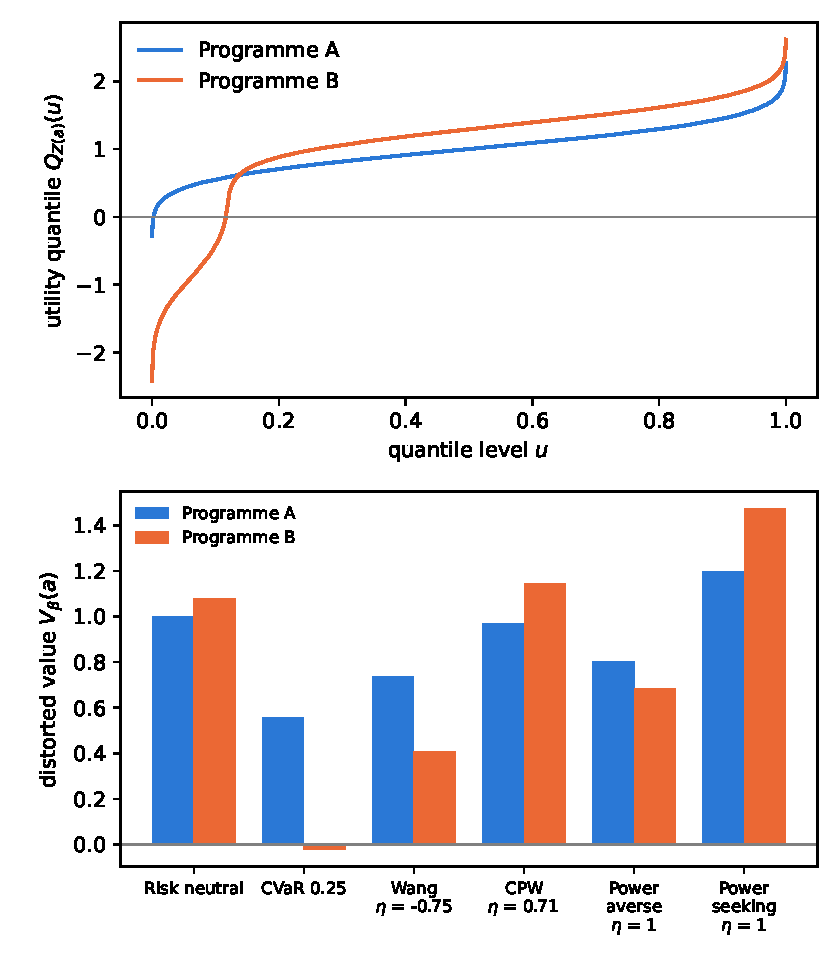
\includegraphics[width=0.92\linewidth]{fig_gbc_distort.pdf}
\caption{Top: quantile functions of utility for two programmes. Bottom: distorted values $\Vbeta$ under six criteria of Table~\ref{gbc:tab:distortions}. B has the higher mean; the three risk averse criteria prefer A.}
\label{gbc:fig:distort}
\end{figure}

\paragraph{Inequality of benefit.} For a nonnegative utility with positive mean, the quantile function also gives the Lorenz curve\index{Lorenz curve|textbf} and Gini coefficient\index{Gini coefficient|textbf} of the benefit,
\[
L_a(p) = \frac{1}{\EU(a)}\int_0^p \Qz(u)\,du,\qquad G(a) = 1 - 2\int_0^1 L_a(p)\,dp .
\]
The bottom fraction $p$ of outcomes holds the fraction $L_a(p)$ of total benefit. Computed from $\Qz$, these mix uncertainty about $\theta$ with differences between recipients: if every recipient gets the same benefit given $\theta$ and $\theta$ is uncertain, $G(a)$ is positive although no recipient is favoured. Computed at each posterior draw from the quantile function of utility across recipients, the Lorenz curve and the Gini coefficient have posterior distributions, and a Gini coefficient that is large with high posterior probability means the benefit is concentrated in few recipients. A planner can trade expected benefit against that coefficient along the frontier the posterior supplies. When utilities can be negative, as for programme B, the Lorenz curve loses its reading as shares of benefit (it can dip below zero, and the Gini coefficient can exceed one), and the conditional value at risk, computed the same way, is the measure of the lower tail.

\subsection{Asymptotics of the policy}\label{gbc:sec:asymptotics}

Let $\Pi$ be a class of policies, $V_\theta(\pi) = \E_\theta[\mathcal{U}(\pi,\theta,Y(\pi))]$ the value of $\pi$ under parameter $\theta$, $\theta_0$ the truth, $\pi_0^\ast = \arg\max_\Pi V_{\theta_0}(\pi)$ the oracle policy and $\hat\pi_N = \arg\max_\Pi \int V_\theta(\pi)\,\pi_N(d\theta)$ the Bayes policy\index{Bayes decision rule!asymptotics of the Bayes policy|textbf}.

\begin{proposition}[Regret of the Bayes policy]\label{gbc:prop:regret}
Suppose that $\sup_{\pi\in\Pi}\lvert V_\theta(\pi) - V_{\theta_0}(\pi)\rvert \le L\,\lVert\theta-\theta_0\rVert$ for all $\theta$, and that the posterior satisfies $\int \lVert\theta-\theta_0\rVert\,\pi_N(d\theta) \le \varepsilon_N$. Then the regret\index{regret|textbf} satisfies
\[
V_{\theta_0}(\pi_0^\ast) - V_{\theta_0}(\hat\pi_N) \le 2L\varepsilon_N .
\]
If moreover $V_{\theta_0}(\pi_0^\ast) - V_{\theta_0}(\pi) \ge c\lVert\pi - \pi_0^\ast\rVert^2$ for all $\pi\in\Pi$, then $\lVert\hat\pi_N - \pi_0^\ast\rVert^2 \le 2L\varepsilon_N/c$.
\end{proposition}
\begin{proof}
Write $\bar V(\pi) = \int V_\theta(\pi)\,\pi_N(d\theta)$. The Lipschitz condition gives $\sup_\pi\lvert\bar V(\pi)-V_{\theta_0}(\pi)\rvert\le L\varepsilon_N$. Since $\hat\pi_N$ maximizes $\bar V$,
\[
\begin{aligned}
V_{\theta_0}(\pi_0^\ast)-V_{\theta_0}(\hat\pi_N)
&\le \bar V(\pi_0^\ast)-\bar V(\hat\pi_N)+2L\varepsilon_N\\
&\le 2L\varepsilon_N.
\end{aligned}
\]
The second claim follows from the margin condition.
\end{proof}

In a regular parametric model the posterior mean of $\lVert\theta-\theta_0\rVert$ is $O_P(N^{-1/2})$ when the tails of the posterior are controlled (contraction at that rate does not give it alone, since a vanishing posterior mass far from $\theta_0$ can keep the mean large), so the regret is $O_P(N^{-1/2})$, the rate of the policy learning bounds of Athey and Wager (2021) for finite complexity classes.

A plug in rule can do better. For incremental value $V_\theta(\pi)=\E[\pi(X)\tau_\theta(X)]$ under a fixed covariate law, with every measurable rule allowed and no budget, the oracle is $\pi_0^\ast(x)=\one\{\tau(x)>0\}$, where $\tau=\tau_{\theta_0}$. If $\bar\tau_N(x)=\E[\tau_\theta(x)\mid D_N]$ satisfies $\sup_x\lvert\bar\tau_N(x)-\tau(x)\rvert\le\delta_N$ and $\tau(X)$ has a bounded density near zero, then $\hat\pi_N(x)=\one\{\bar\tau_N(x)>0\}$ disagrees with the oracle only where $\lvert\tau(X)\rvert\le\delta_N$, and loses $\lvert\tau(X)\rvert$ there, so
\[
\begin{aligned}
V_{\theta_0}(\pi_0^\ast)-V_{\theta_0}(\hat\pi_N)&=\E\bigl[\lvert\tau(X)\rvert\,\one\{\hat\pi_N(X)\ne\pi_0^\ast(X)\}\bigr]\\
&\le\delta_N\Prob\{\lvert\tau(X)\rvert\le\delta_N\}=O(\delta_N^2),
\end{aligned}
\]
the fast rate of plug in classifiers (Audibert and Tsybakov 2007).

When $\theta$ is infinite dimensional the condition can still hold in a suitable norm: for the incremental value $V_\theta(\pi)=\int\pi(x)\tau_\theta(x)\,H(dx)$ over a covariate law $H$, every policy with $0\le\pi\le1$ satisfies $\lvert V_\theta(\pi)-V_{\theta_0}(\pi)\rvert\le\lVert\tau_\theta-\tau_{\theta_0}\rVert_{L^1(H)}$, so $L=1$ however rich the policy class. The rate then rests on how fast the posterior mean of that distance shrinks, which depends on the prior and the smoothness of the effect surface (Ghosal and van der Vaart 2017).

\subsection{Worked examples}\label{gbc:sec:examples}



\subsubsection{Normal learning}\label{gbc:sec:normal}

Let $Y_i\mid\theta\sim N(\theta,\sigma^2)$ with $\sigma$ known, $\theta\sim N(\mu_0,\sigma_0^2)$, and the action be a report $a$ with utility $-(a-\theta)^2$. The posterior is $N(\mu_N,\sigma_N^2)$ with
\[
\mu_N = \frac{\mu_0/\sigma_0^2 + N\bar Y/\sigma^2}{1/\sigma_0^2 + N/\sigma^2},\qquad
\sigma_N^2 = \Bigl(\frac{1}{\sigma_0^2} + \frac{N}{\sigma^2}\Bigr)^{-1}.
\]
The Bayes action is $a^\ast=\mu_N$ with posterior expected loss $\sigma_N^2 = O(N^{-1})$. The loss $(a^\ast-\theta)^2$ is $\sigma_N^2$ times a chi squared variable on one degree of freedom, so its upper quantiles, which concern a risk averse reporter, come from the same draws as the mean.

The example is trivial as inference and useful as a check. At the sufficient summary $s=\bar Y$ the posterior quantile function is $\mu_N(s)+\sigma_N\Phi^{-1}(u)$, the closed form used to check the network in Section~\ref{comp:sec:network}. Check conjugate special cases before trusting the computation elsewhere; when none exists, use simulation based calibration (Section~\ref{comp:sec:checks}).

The same check can be run on a decision. Take a two arm trial with $n$ patients per arm, independent uniform priors on the success rates $p_0$ and $p_1$, and $K_w$ successes in arm $w$. The posterior of $\tau=p_1-p_0$ is the difference of independent $\mathrm{Beta}(K_1+1,n-K_1+1)$ and $\mathrm{Beta}(K_0+1,n-K_0+1)$ variables, and the value of treating, $\CVaR_\eta(\tau\mid D)-c$ against zero for not treating, can be computed by numerical integration; refining the integration grid moved it by at most $2.5\times10^{-4}$ in 200 checks for each $n$. We trained the network of Section~\ref{comp:sec:network} with the check loss on 300{,}000 simulated trials, 100{,}000 for each of $n=25$, 100 and 400, with $n$, $K_0$ and $K_1$ as inputs, for 40 passes and with five seeds, sorted its quantiles on 1{,}000 levels and read off the value for $\eta\in\{0.05,0.1,0.25,1\}$ and $c\in\{0,0.05,0.2\}$. On 10{,}000 fresh trials for each $n$, the same for all five seeds, the root mean squared error of the value at $\eta=0.05$ is 0.022 at $n=25$ and 0.005 at $n=400$, and about 0.002 at $\eta=1$, the posterior mean, with a spread across seeds of a tenth to a fifth of the error. Averaged over seeds, the network's action differs from the exact Bayes action in at most 2.3 percent of these trials (3.5 percent for the worst seed), at an average cost of about $3\times10^{-4}$ or less in the risk difference. Close calls are another matter. On separate samples of close calls, up to 1{,}000 count pairs for each $n$, $\eta$ and $c$ whose exact value lies within 0.02 of zero, the network's action under the tail criteria ($\eta<1$) differs from the exact one in 5 to 13 percent of trials at $n=400$, 10 to 21 percent at $n=100$ and 12 to 58 percent at $n=25$, where only 16 to 25 count pairs qualify; the average cost on those trials is at most 0.006. Before sorting, every curve crossed somewhere. The largest dip is typically 3 to 8 percent of the posterior sd, but in the worst trial at $n=400$ it is 1.1 to 1.4 sd, depending on the seed, because the posterior narrows with $n$ and the network's wobble does not. This is one conjugate design, a finite check on Problem 13 of Chapter~\ref{ch:open}, not a calibration result for the method.

\subsubsection{A stylized supplement trial}

In the Lanarkshire milk experiment\index{Lanarkshire milk experiment} (Section~\ref{sec:milk}), teachers' discretion in assigning children to milk or control left the controls taller and heavier at the start. Consider a stylized version in which $Z_i$ measures how undernourished child $i$ is at baseline, $W_i$ indicates supplementation, and
\[
Y_i(w) \sim N(\mu_w + \alpha_w Z_i, \sigma^2),\qquad \Prob(W_i=1\mid Z_i) = \expit(\gamma_0 + \gamma_1 Z_i),
\]
with $\gamma_1>0$ representing teachers who favour needier children. Because assignment depends on $Z$, the raw contrast is confounded, while the conditional model identifies $\tau(z) = (\mu_1-\mu_0) + (\alpha_1-\alpha_0)z$. From one network trained on prior simulations, GBC returns the posterior of the average effect over any chosen population of children, the posterior of $\tau(z)$, and the Bayes targeting rule $\one\{\E[\tau(z)\mid D] > \lambda\}$ for a cost $\lambda$ per child. If the posterior puts $\alpha_1-\alpha_0>0$, so that benefit grows with undernourishment, the rule treats children above a threshold of need; under CVaR the threshold moves to protect the children whose benefit is most uncertain. 

\subsubsection{Smoking and the probability of causation}

Let $W$ indicate heavy smoking and $Y$ lung cancer. The probability of necessity\index{probability of necessity}, $\PN = \Prob(Y(0)=0\mid W=1, Y=1)$, the probability that a smoker's cancer would not have occurred without smoking, is not point identified (Chapter~\ref{ch:tianpearl}). Under exogeneity of $W$, Tian and Pearl (2000) give the sharp bounds
\[
\max\Bigl\{0,\ 1 - \frac{1}{\mathrm{RR}}\Bigr\} \le \PN \le \min\Bigl\{1,\ \frac{\Prob(Y=0\mid W=0)}{\Prob(Y=1\mid W=1)}\Bigr\},
\]
where
\[
\mathrm{RR} = \frac{\Prob(Y=1\mid W=1)}{\Prob(Y=1\mid W=0)},
\]
and without exogeneity they combine observational and experimental distributions as in Chapter~\ref{ch:tianpearl}. A posterior for the cell probabilities induces one for the bounds, and a prior on the unidentified coupling of $Y(0)$ and $Y(1)$ induces a posterior for $\PN$ itself. Since exogeneity is exactly what Fisher disputed, an honest analysis reports the bounds under exogeneity alongside the sensitivity analysis of Section~\ref{sec:sensitivity}. A court asking whether smoking caused a particular plaintiff's cancer needs this quantity, not the average effect.

In GBC the computation is direct. The summary is the two by two table of smoking and cancer counts, or the four cell proportions with the sample size. The network learns the joint posterior of the cell probabilities and the potential outcome coupling through the triangular map of Section~\ref{comp:sec:noise}. Each joint draw gives both bounds from the cells and $\PN$ from the cells and coupling, so all three posteriors come from the same draws with no further training. A network trained on $\PN$ alone would not supply the bounds. Under the court's more probable than not standard and equal losses for the two wrong findings, the Bayes rule finds causation when the posterior mean $\E[\PN\mid D]$ exceeds one half. The posterior probability that $\PN$ exceeds one half answers a different question, about the population parameter, closer to the rule some courts apply that the relative risk must exceed two (under exogeneity and monotonicity $\PN=1-1/\mathrm{RR}$, so $\PN>1/2$ exactly when $\mathrm{RR}>2$). Both are reported under exogeneity, each with how far it moves as the sensitivity parameter of Section~\ref{sec:sensitivity} is varied. A point estimate of the relative risk, however precise, does not answer the question put to the witness.

\subsubsection{Targeting under a budget and portfolio choice}

For the budget rule\index{Bayes decision rule!treatment allocation} of Section~\ref{cdt:sec:targeting}, replacing posterior means by the CVaR at level $0.1$ ranks units by expected benefit in the worst tenth of posterior outcomes, a criterion for a planner wary of harming a group. It is a separable criterion, the sum over treated units of each unit's CVaR, and not the CVaR of total benefit, because CVaR is not additive. With three equal groups whose effects are $(0,4)$, $(4,0)$ and $(1,1)$ in two equally likely posterior states and a budget for two groups, ranking by CVaR treats the third group and one other, for a total benefit whose CVaR is 1, while treating the first two gives a certain total of 4. The CVaR of total benefit needs joint posterior draws of the effects across groups.

The mean ranking favours a group with a large but uncertain effect, because it is small or poorly represented in the data; the CVaR favours one with a modest, well determined effect. Each rule is optimal for its own criterion. Both rankings, their expected benefits and their Lorenz curves come from one set of posterior draws, in GBC from one trained network evaluated at the observed summary, so the planner can see the cost in expected benefit of the protection the CVaR rule buys. Chapter~\ref{ch:gente} develops the heterogeneous effect model that supplies $\tau(x)$.

\paragraph{Portfolio choice.} Let $\theta = (\mu,\Sigma)$ be the mean and covariance of log returns $r$ on $K$ assets, with gross returns $R = \exp(r)$ taken coordinatewise, and let an investor choose long only weights $w$ ($w_k\ge0$ and $\sum_k w_k=1$, so that $w^\top R>0$) to maximize the expected power utility $\{(w^\top R)^\alpha-1\}/\alpha$ of gross portfolio return, with $\alpha<1$ and $\alpha\ne0$. Its limit as $\alpha\to0$ is logarithmic utility, the Kelly criterion, and $\alpha<0$, a relative risk aversion $1-\alpha$ above one, gives a more cautious allocation than Kelly. GBC simulates triples $(\theta,D,R)$ from the prior and model, with $D$ a history of returns, and learns the quantile function of utility given the summary of $D$ for each $w$ on a grid; evaluated at the observed history it gives the posterior predictive law of utility. The Wang distortion with $\eta<0$ yields a portfolio that hedges left tail returns while keeping upside, and the conditional value at risk a portfolio judged by the mean of its worst outcomes, both from the same network. Over a continuous set of weights, the representation $\CVaR_\eta(Z)=\max_t\{t-\eta^{-1}\E[(t-Z)_+]\}$ of Rockafellar and Uryasev (2000), computed from posterior predictive draws of $R$, makes the CVaR choice one concave maximization over $w$ and $t$, since utility is concave in $w$.

\subsection{Dynamic treatment regimes}\label{gbc:sec:dynamic}

With repeated decisions\index{dynamic treatment regime}, each period's transitions are causal: $p(X_{t+1}, Y_t\mid X_t, \mathrm{do}(W_t=a);\theta)$, with reward $\mathcal{U}(a,\theta,Y_t(a))$ and discount $\gamma\in[0,1)$. The g formula of Chapter~\ref{ch:frameworks} identifies the transitions under sequential ignorability. The parameter $\theta$ is fixed but unknown, and that persistence matters. Given $\theta$, the problem is a Markov decision process with value $V_\theta^\pi$ for policy $\pi$. The Bayes value of a policy that does not learn further is $\int V^\pi_\theta(s)\,\pi_N(d\theta)$, estimated by simulating whole trajectories, each with one posterior draw of $\theta$ held fixed, and averaging over draws. A policy that also learns from the outcomes it generates solves a Bayes adaptive decision process\index{Bayes adaptive decision process|textbf} whose state pairs the current covariates with the current posterior, $s_1=(X_1,\pi_N)$ in the first period. With $H_2=(s_1,w_1,Y_1,X_2)$ the history after the first action and $\mathcal{U}_t$ the utility in period $t$, a two period problem gives
\[
\begin{aligned}
Q_2(h_2,w_2) &= \E\bigl[\mathcal{U}_2\mid h_2,\mathrm{do}(w_2)\bigr],\\
Q_1(s_1,w_1) &= \E\Bigl[\mathcal{U}_1 + \gamma\max_{w_2}Q_2(H_2,w_2)\Bigm| s_1,\mathrm{do}(w_1)\Bigr],
\end{aligned}
\]
where $h_2$ is a realized value of $H_2$ and the expectation in $Q_2$ is over $\theta\sim\pi(\theta\mid D_N,h_2)$, the posterior updated by the first period's outcome. GBC suits this well when the training simulations include the first period's outcome and the summary records it and the sample size: updating on $h_2$ is then one more evaluation of the network, with no new chain. A network trained for a fixed sample size returns the wrong posterior spread.

A common shortcut averages the transition law over the current posterior and solves one Markov decision process with the operator
\[
(\mathcal T Q)(s,a) = \E_{\theta\sim\pi_N}\E\bigl[R(s,a;\theta) + \gamma\max_{a'} Q(S',a')\mid s,\mathrm{do}(a),\theta\bigr],
\]
a contraction in the supremum norm with modulus $\gamma$ when rewards are bounded. Its fixed point is the value of the posterior mean process, as if $\theta$ were redrawn every period. It ignores the persistence of $\theta$ and the value of learning, and should be checked against trajectory simulation. Replacing expectations by distorted values at each stage gives risk sensitive dynamic policies, but distorted criteria are not in general time consistent\index{risk sensitive decisions!time consistency}, so stagewise and whole horizon versions can differ.



% moved to Chapter~\ref{ch:open}: the subsection "Open problems" is now Problems 11 to 14

% In practice section moved here from the front of the chapter (comp phase 1)
\section{In practice}

\paragraph{The target.} The target of an economic decision is the causal expected utility \eqref{cdt:eq:bayes}: the utility of an action averaged over the interventional predictive and over the posterior of the structural parameters. Every quantity in this chapter is a functional of that posterior and inherits its properties: efficiency in the nonparametric model depends on the prior, for instance a propensity aware one (Part~III), not on computation or on the choice of criterion.

\paragraph{What the analyst does differently.} Before fitting, the analyst states the regime and which parameters are invariant to the policy change. She fits a posterior over those parameters and simulates the counterfactual policy forward (Section~\ref{cdt:sec:lucas}). She treats continuity at the threshold, parallel trends and exclusion as modelling assumptions with a sensitivity analysis rather than as labels. And she reports the probability that the decision is right, the acceptability curve across $\lambda$ and the posterior of $\tau(x)$ over the population to be treated, not an interval for a ratio of means.

\paragraph{Against DML.} Double machine learning estimates one reduced form contrast under the historical regime, and estimates it well: for an average effect in a large cross section with no policy change in view, its interval is adequate and cheaper than a structural posterior. A merger, a change in a Taylor rule coefficient or a carbon tax is a regime the data have never visited, and only a model of the invariant parameters predicts it. A risk neutral targeting rule needs only the sign of $\tau(x)$ against a threshold, and policy learning with cross fitted doubly robust scores (Athey and Wager 2021), or the R learner of Nie and Wager (2021) for $\tau(x)$ itself, delivers it without a posterior. The posterior adds the lower tail of $\tau(x)$ for a planner who will not risk harming a group, the joint posterior of $\Delta E$ and $\Delta C$ for the cost effectiveness decision, the distorted values of Section~\ref{gbc:sec:risk}, which can reverse the ranking the mean gives, and the probability that each decision is right. None of these is the contrast that a DML score estimates. With homogeneous effects, a fixed regime and squared error loss, DML and the posterior mean agree to first order in large samples if the posterior satisfies a semiparametric Bernstein von Mises theorem at the efficient variance in DML's model (Section~\ref{pg:sec:bvm}) and its rescaled draws $\sqrt N(\tau-\hat\tau_N)$, centred at the efficient estimator $\hat\tau_N$, are uniformly integrable in probability. Total variation convergence alone does not control the posterior mean. The prior can separate them in small samples. Their costs are comparable in the designs timed in Section~\ref{comp:sec:cost}, with DML ahead when covariates are numerous. When a decision turns on a probability, as the court's question about the probability of necessity does, the posterior supplies it.

\section*{Notes}



Dhaene and coauthors (2012) remark on quantiles and distortion risk measures. The sources for the quantile network, its check loss, distributional reinforcement learning and optimal transport are in the Notes of Chapter~\ref{ch:computation}.

\begin{exercises}
\item\label{ex:chcdt:1} In Newcomb's problem let the predictor be correct with probability $p$ whichever act the agent takes, let the opaque box contain $M$ if one box is predicted, let the transparent box contain $m<M$, and let $q$ be the agent's credence that the opaque box is full. Compute evidential and causal expected utilities of each act and find the values of $p$ for which the two theories disagree.
\item\label{ex:chcdt:2} In the twin prisoner's dilemma with payoffs $(R,S,T,P)$, $T>R>P>S$, show that causal reasoning recommends defection for any belief about the twin, and, if the twin matches the agent's act with probability $p$ whichever act she takes, find the value of $p$ above which evidential reasoning recommends cooperation.
\item\label{ex:chcdt:3} Show that the set of correlated equilibria of a finite game is a convex polytope, and that it contains every mixed Nash equilibrium.
\item\label{ex:chcdt:4} A treatment has posterior net monetary benefit $\lambda\Delta E - \Delta C$ with $\Delta E\sim N(0.2, 0.1^2)$ and $\Delta C\sim N(5000, 2000^2)$ independent. Plot the probability of positive net benefit against $\lambda$ and compare the decision with the one based on the ratio of posterior means.
\item\label{ex:chcdt:5} Explain why the Lucas critique is a failure of modularity in the sense of Chapter~\ref{ch:blp}, and state the modularity assumption for a change in a Taylor rule coefficient.

\item\label{ex:chgbc:1} Prove that $\E[Z] = \int_0^1 Q_Z(u)\,du$ for any integrable $Z$, and that for $\beta(u)=\eta u$ the distorted value is $\eta^{-1}\int_0^\eta Q_Z(u)\,du$.
\item\label{ex:chgbc:2} Show that the Wang distortion with $\eta<0$ satisfies $\beta(u)\le u$ and that, for $Z\sim N(m,s^2)$, $\Vbeta = m + \eta s$.
\item\label{ex:chgbc:4} Compute the CVaR of programmes A and B at each level $\eta$, from simulated draws of the two utilities described in the text, and find the level at which the planner is indifferent between them. Compare it with the value computed from the exact distributions of the two programmes.
\item\label{ex:chgbc:5} Show by example that a distorted criterion applied stage by stage in a two period problem can choose a different first period action from the same criterion applied to total utility.
\end{exercises}

\chapter[The Causal Effect of a Merger]{The Causal Effect of a Merger: Bayesian BLP Demand Estimation}\label{ch:blp}

\providecommand{\E}{\mathbb{E}}
\providecommand{\diag}{\mathrm{diag}}
\providecommand{\cH}{\mathcal{H}}
\providecommand{\data}{\mathcal{D}}
\newcommand{\numcorrLa}{0.58}
\newcommand{\numconductacc}{0.98}
\newcommand{\numcovnaive}{0.85}
\newcommand{\numncal}{354}
\newcommand{\numcovavg}{0.94}
\newcommand{\numcovmin}{0.91}
\newcommand{\numpgbcx}{0.98}
\newcommand{\numplogitx}{0.98}
\newcommand{\numpgbcxii}{0.77}
\newcommand{\numplogitxii}{0.47}
\newcommand{\numpgbcxv}{0.08}
\newcommand{\numplogitxv}{0.02}
\newcommand{\numldir}{0.437}
\newcommand{\numldirsd}{0.035}
\newcommand{\numdpdir}{13.0}
\newcommand{\numdpdirsd}{1.5}
\newcommand{\numcsdir}{-0.149}
\newcommand{\numcsdirsd}{0.024}
\newcommand{\numltrue}{0.434}
\newcommand{\numdptrue}{13.3}
\newcommand{\numcstrue}{-0.150}
\newcommand{\numspmicro}{0.047}
\newcommand{\numspnomicro}{0.088}
\newcommand{\numpbert}{1.000}
\newcommand{\numjmracc}{0.16}
\newcommand{\numpharm}{1.00}
\newcommand{\numdplogit}{12.1}
\newcommand{\numinsideshare}{0.60}
\newcommand{\nummeanprice}{3.46}
\newcommand{\numguppia}{1.00}
\newcommand{\numguppib}{1.00}
\newcommand{\numguppic}{1.00}
\newcommand{\numguppid}{1.00}

\newcommand{\nummcnxl}{500}
\newcommand{\nummcboundxl}{4}
\newcommand{\nummcexplxl}{4}
\newcommand{\nummcsprmsegmmxl}{0.111}
\newcommand{\nummcsprmsegbcxl}{0.040}
\newcommand{\nummcspcovgmmxl}{0.95}
\newcommand{\nummcspcovgbcxl}{0.98}
\newcommand{\nummcsprmsenmxl}{0.094}
\newcommand{\nummcspcovnmxl}{0.95}
\newcommand{\nummcsplengbcxl}{0.18}
\newcommand{\nummcsplengmmxl}{0.34}
\newcommand{\nummcsprmseplugxl}{0.111}
\newcommand{\nummcspbiasgmmxl}{-0.022}
\newcommand{\nummcspbiasplugxl}{-0.022}
\newcommand{\nummcsprmsesegmmxl}{0.004}
\newcommand{\nummcsprmsesegbcxl}{0.001}
\newcommand{\nummcdprmsegmmxl}{3.787}
\newcommand{\nummcdprmsegbcxl}{1.131}
\newcommand{\nummcdpcovgmmxl}{0.92}
\newcommand{\nummcdpcovgbcxl}{0.99}
\newcommand{\nummcdprmsenmxl}{1.541}
\newcommand{\nummcdpcovnmxl}{0.97}
\newcommand{\nummcdplengbcxl}{5.64}
\newcommand{\nummcdplengmmxl}{5.84}
\newcommand{\nummcdprmseplugxl}{1.838}
\newcommand{\nummcdpbiasgmmxl}{0.365}
\newcommand{\nummcdpbiasplugxl}{-0.109}
\newcommand{\nummcdprmsesegmmxl}{0.952}
\newcommand{\nummcdprmsesegbcxl}{0.031}
\newcommand{\nummccovsexl}{0.013}
\newcommand{\nummclercovgmmxl}{0.86}
\newcommand{\nummclercovgbcxl}{0.99}
\newcommand{\nummclercovsegmmxl}{0.016}
\newcommand{\nummcfivexln}{500}
\newcommand{\nummcfivexlbound}{279}
\newcommand{\nummcfivesprmsegmmxl}{0.132}
\newcommand{\nummcfivesprmsegbcxl}{0.024}
\newcommand{\nummcfivespcovgmmxl}{0.84}
\newcommand{\nummcfivespcovgbcxl}{1.00}
\newcommand{\nummcfivedprmsegmmxl}{16.898}
\newcommand{\nummcfivedprmsegbcxl}{1.331}
\newcommand{\nummcfivedpcovgmmxl}{0.52}
\newcommand{\nummcfivedpcovgbcxl}{0.98}
\newcommand{\nummcnxv}{500}
\newcommand{\nummcboundxv}{49}
\newcommand{\nummcexplxv}{48}
\newcommand{\nummcsprmsegmmxv}{0.184}
\newcommand{\nummcsprmsegbcxv}{0.059}
\newcommand{\nummcspcovgmmxv}{0.94}
\newcommand{\nummcspcovgbcxv}{0.96}
\newcommand{\nummcsprmsenmxv}{0.097}
\newcommand{\nummcspcovnmxv}{0.98}
\newcommand{\nummcsplengbcxv}{0.25}
\newcommand{\nummcsplengmmxv}{0.49}
\newcommand{\nummcsprmseplugxv}{0.184}
\newcommand{\nummcspbiasgmmxv}{-0.053}
\newcommand{\nummcspbiasplugxv}{-0.053}
\newcommand{\nummcsprmsesegmmxv}{0.006}
\newcommand{\nummcsprmsesegbcxv}{0.002}
\newcommand{\nummcdprmsegmmxv}{96.640}
\newcommand{\nummcdprmsegbcxv}{1.696}
\newcommand{\nummcdpcovgmmxv}{0.88}
\newcommand{\nummcdpcovgbcxv}{0.95}
\newcommand{\nummcdprmsenmxv}{2.012}
\newcommand{\nummcdpcovnmxv}{0.95}
\newcommand{\nummcdplengbcxv}{7.32}
\newcommand{\nummcdplengmmxv}{6.98}
\newcommand{\nummcdprmseplugxv}{2.346}
\newcommand{\nummcdpbiasgmmxv}{9.296}
\newcommand{\nummcdpbiasplugxv}{-0.009}
\newcommand{\nummcdprmsesegmmxv}{46.805}
\newcommand{\nummcdprmsesegbcxv}{0.064}
\newcommand{\nummccovsexv}{0.013}
\newcommand{\nummclercovgmmxv}{0.76}
\newcommand{\nummclercovgbcxv}{1.00}
\newcommand{\nummclercovsegmmxv}{0.019}
\newcommand{\nummcfivexvn}{498}
\newcommand{\nummcfivexvbound}{291}
\newcommand{\nummcfivesprmsegmmxv}{0.147}
\newcommand{\nummcfivesprmsegbcxv}{0.029}
\newcommand{\nummcfivespcovgmmxv}{0.87}
\newcommand{\nummcfivespcovgbcxv}{1.00}
\newcommand{\nummcfivedprmsegmmxv}{22.132}
\newcommand{\nummcfivedprmsegbcxv}{1.158}
\newcommand{\nummcfivedpcovgmmxv}{0.43}
\newcommand{\nummcfivedpcovgbcxv}{1.00}
\newcommand{\nummscollusionalpha}{1.03}
\newcommand{\nummscollusiontrue}{0.0}
\newcommand{\nummscollusiongmm}{9.0}
\newcommand{\nummscollusiongbc}{0.0}
\newcommand{\nummscollusionltrue}{0.572}
\newcommand{\nummscollusionlgmm}{0.347}
\newcommand{\nummscollusionlgbc}{0.605}
\newcommand{\nummscollusionpc}{1.000}
\newcommand{\nummsperfectalpha}{0.97}
\newcommand{\nummsperfecttrue}{0.0}
\newcommand{\nummsperfectgmm}{38.4}
\newcommand{\nummsperfectgbc}{0.0}
\newcommand{\nummsperfectltrue}{0.000}
\newcommand{\nummsperfectlgmm}{0.900}
\newcommand{\nummsperfectlgbc}{0.000}
\newcommand{\nummsperfectpc}{1.000}
\newcommand{\nummspartgmmbiasdp}{3.25}
\newcommand{\nummspartgmmrmsedp}{3.74}
\newcommand{\nummspartgmmbiasler}{-0.126}
\newcommand{\nummspartgmmrmseler}{0.129}
\newcommand{\nummspartgmmsedp}{0.19}
\newcommand{\nummspartgbcbiasdp}{2.99}
\newcommand{\nummspartgbcrmsedp}{3.58}
\newcommand{\nummspartgbcbiasler}{-0.108}
\newcommand{\nummspartgbcrmseler}{0.118}
\newcommand{\nummspartgbcsedp}{0.20}
\newcommand{\nummsparttruedp}{7.10}
\newcommand{\nummsparttruebertdp}{10.81}
\newcommand{\nummsparttrueler}{0.507}
\newcommand{\nummspartn}{100}
\newcommand{\nummspartpcbert}{0.93}
\newcommand{\nummspartpccoll}{0.07}
\newcommand{\nummspartpcperf}{0.00}

\newcommand{\numcerdpmtrue}{8.6}
\newcommand{\numcerdprtrue}{3.2}
\newcommand{\numcerdpmgbc}{9.0}
\newcommand{\numcerdpmgbcsd}{1.4}
\newcommand{\numcerdprgbc}{3.0}
\newcommand{\numcerdprgbcsd}{1.3}
\newcommand{\numcerdpmgmm}{7.1}
\newcommand{\numcerdprgmm}{2.7}
\newcommand{\numcerdpmgmmsd}{1.0}
\newcommand{\numcerdprgmmsd}{0.4}
\newcommand{\numcerdpmlogit}{6.7}
\newcommand{\numcerdprlogit}{2.6}
\newcommand{\numcerpmgbc}{1.00}
\newcommand{\numcerprgbc}{0.01}
\newcommand{\numcerpmgmm}{1.00}
\newcommand{\numcerprgmm}{0.00}
\newcommand{\numcercsmtrue}{-0.079}
\newcommand{\numcercsrtrue}{-0.044}
\newcommand{\numcercsmgbc}{-0.081}
\newcommand{\numcercsrgbc}{-0.042}
\newcommand{\numcerltrue}{0.431}
\newcommand{\numcerlgbc}{0.422}
\newcommand{\numcershA}{19.6}
\newcommand{\numcershB}{12.3}
\newcommand{\numcershC}{15.4}
\newcommand{\numcershD}{8.7}
\newcommand{\numcerinside}{56.1}
\newcommand{\numcerprgbcnabove}{10}
\newcommand{\numcerngbcdraws}{1{,}500}
\newcommand{\numcerdprgbcqlo}{1.95}
\newcommand{\numcerdprgbcqhi}{4.14}
\newcommand{\numcerdprgmmqlo}{2.43}
\newcommand{\numcerdprgmmqhi}{3.55}


\begin{tcolorbox}[colback=gray!6,colframe=gray!50,title=In brief,fonttitle=\normalfont\itshape,coltitle=black,colbacktitle=gray!15,boxrule=0.4pt,arc=1pt]
A merger is the intervention $\mathrm{do}(H := H^{\mathrm{post}})$ on the form of competition, with no treated unit, so its price effect can only come from a model. Under modularity and given the premerger data, it depends on the three nonlinear demand parameters and the form of competition alone, and the agency's answer is a pushforward posterior. Markups are the hinge: the Lerner index, upward pricing pressure and the merger price effect follow from the markup map, and diversion from the demand parameters. Orthogonal moments fall short here, because the target is a nonlinear fixed point, the moments are flat at zero heterogeneity, conduct is a discrete parameter and the decision needs a probability. Generative Bayesian computation simulates industries and learns the posterior of the estimands and of conduct from summary statistics. With 15 markets, over \nummcnxv{} simulated industries at one true parameter value and on the same aggregate data, its root mean squared error for the merger price effect is \nummcdprmsenmxv{} percentage points against \nummcdprmseplugxv{} for the usual BLP moment estimator at its point estimate, whose Krinsky and Robb draws explode in \nummcexplxv{} of those industries. In one simulated collusive industry that estimator predicts a \nummscollusiongmm\% price rise where the truth is \nummscollusiontrue\%, while the posterior puts probability \nummscollusionpc{} on collusion. The applications are a minivan merger and a cereal merger with a divestiture remedy.
\end{tcolorbox}

A merger\index{merger|textbf} is a treatment applied once, to one industry, and never at random. The competition authority must predict its effect on prices before it happens, when the merged industry does not yet exist. If the fundamental problem of causal inference is that we never see both potential outcomes for the same unit, merger review is its limiting case: we see neither the treated outcome nor any treated unit.

The only route to the answer is a model of how the treatment works. A merger changes who sets which prices, and prices move because firms reoptimize in a new equilibrium. The causal effect is a function of model parameters and its posterior is the object of inference. The question is how to compute that posterior when the model is an equilibrium of a random coefficients demand system.

The workhorse model is the random coefficients logit\index{random coefficients logit|textbf} of Berry, Levinsohn and Pakes (1995)\index{Berry Levinsohn Pakes model|see{BLP demand model}}, known as BLP\index{BLP demand model|textbf}\index{BLP|see{BLP demand model}}. It is estimated by the generalized method of moments (GMM), and its estimates feed the merger simulations\index{merger simulation|textbf}, diversion ratios and upward pricing pressure\index{upward pricing pressure} screens of agencies and courts (Nevo 2000; Farrell and Shapiro 2010; Miller and Weinberg 2017). We develop a Bayesian alternative organized around one fact: every antitrust\index{antitrust|textbf} quantity is a function of the markup vector and the demand parameters, and the markup vector, given the data, depends on only two unknowns: the nonlinear demand parameters $\theta_2$ and the form of competition $H$.

We use generative Bayesian computation\index{generative Bayesian computation} (GBC) to learn the posterior.

\section{The merger as an intervention}\label{blp:sec:causal}

We define potential prices\index{potential prices|textbf} under each form of competition and state modularity, the assumption that carries the premerger estimates to the merger counterfactual. Modularity is not enough: the nonlinear demand parameters and conduct must themselves be identified, through the instruments and the separation results of the chapter. The payoff is Proposition~\ref{blp:prop:ident}: given the data, the price effect of a merger depends only on three nonlinear demand parameters and a discrete conduct parameter, so the agency's question is a question about the posterior of $(\theta_2,H)$.

\subsection{Potential prices and the structural causal model}

Index markets by $t=1,\dots,T$ and products by $j=1,\dots,J$. An ownership structure, or more
generally a conduct, is a matrix $H$ in a finite set $\cH$ (Section~\ref{blp:sec:model}), except that perfect competition enters as a label $H^P$ for zero markups. For each $h\in\cH$ write $\bm p_t(h)$ and $\bm s_t(h)$ for the prices
and shares that market $t$ would exhibit if conduct were $h$. These are potential outcomes\index{potential outcomes} in the
sense of Rubin (1974). We observe $\bm p_t = \bm p_t(H)$ for the prevailing $H$; a merger that changes conduct to $H^{\mathrm{post}}$ has causal effect
\[
\Delta\bm p_t \;=\; \bm p_t(H^{\mathrm{post}}) - \bm p_t(H).
\]
No market has ever been observed under $H^{\mathrm{post}}$.

Potential prices\index{potential prices} are generated by a structural causal model\index{structural causal model}\index{structural causal model!of the merger|textbf} in the sense of Pearl (2009). Exogenous variables are product characteristics $\bm x_t$, cost shifters\index{cost shifter|textbf} $\bm w_t$, unobserved
demand shocks\index{demand shock|textbf} $\bm\xi_t$ (quality the econometrician does not see) and cost shocks $\bm\omega_t$.
The structural equations are
\begin{equation}\label{blp:eq:scm}
\delta_t = \bm x_t^\top\beta + \bm\xi_t,\qquad
\bm c_t = \bm w_t^\top\gamma + \bm\omega_t,\qquad
(\bm p_t,\bm s_t) = \mathrm{Eq}(\delta_t,\bm x_{1t},\bm c_t;\theta_2,H),
\end{equation}
where $\mathrm{Eq}$ returns the equilibrium of the pricing game with demand $\theta_2$, mean
utilities $\delta_t$, the characteristic $\bm x_{1t}$ that carries the random coefficient, marginal costs\index{marginal cost|textbf} $\bm c_t$ and conduct $H$; we assume this equilibrium is unique, or that $\mathrm{Eq}$ applies a fixed selection rule. A merger is the intervention\index{merger!as an intervention|textbf}
$\mathrm{do}(H := H^{\mathrm{post}})$\index{do operator}. Figure~\ref{blp:fig:dag} draws the graph.

\begin{figure}[htbp]
\centering
\begin{tikzpicture}[
  node distance=1.1cm and 1.5cm,
  v/.style={circle, draw=#1, fill=#1!12, very thick, minimum size=0.95cm, font=\small},
  u/.style={circle, draw=#1, fill=#1!12, very thick, dashed, minimum size=0.95cm, font=\small},
  arr/.style={-{Stealth[length=2.4mm]}, very thick, draw=black!60}]
\node[v=gbc] (x) {$\bm x$};
\node[u=jmr, below=of x] (xi) {$\bm\xi$};
\node[v=aqua, below=of xi] (w) {$\bm w$};
\node[u=jmr, below=of w] (om) {$\bm\omega$};
\node[v=gbc, right=2.2cm of x] (d) {$\delta$};
\node[v=aqua, right=2.2cm of w] (c) {$\bm c$};
\node[v=sand, right=2.0cm of $(d)!0.5!(c)$] (p) {$\bm p$};
\node[v=gbc, right=1.6cm of p] (s) {$\bm s$};
\node[v=jmr, above=2.9cm of p] (H) {$H$};
\node[font=\footnotesize, text=black!60, right=0.1cm of H] {$\mathrm{do}(H := H^{\mathrm{post}})$};
\draw[arr] (x) -- (d); \draw[arr] (xi) -- (d); \draw[arr] (w) -- (c); \draw[arr] (om) -- (c);
\draw[arr] (d) -- (p); \draw[arr] (c) -- (p); \draw[arr] (H) -- (p); \draw[arr] (p) -- (s);
\draw[arr] (d) to[bend left=22] (s);
\end{tikzpicture}
\caption{The structural causal model of a differentiated products market. Dashed nodes are
unobserved. The demand shock $\bm\xi$ moves both prices (through the equilibrium) and shares, so
it confounds the effect of price on demand; the cost shifter $\bm w$ moves prices only through
costs and is an instrument. A merger is the intervention $\mathrm{do}(H := H^{\mathrm{post}})$. The graph omits four paths of the model: the correlation between $\bm\xi$ and $\bm\omega$ and the dependence of cost on the characteristic $x_1$, both of which the simulations use (Section~\ref{blp:sec:model}), and the direct effects of $x_1$ on prices and shares through its random coefficient.}
\label{blp:fig:dag}
\end{figure}

\begin{assumption}[Modularity]\label{blp:ass:mod}
The intervention $\mathrm{do}(H := H^{\mathrm{post}})$ replaces $H$ in the equilibrium equation of
\eqref{blp:eq:scm} and leaves the other structural equations, the parameters $(\beta,\gamma,\theta_2)$
and the exogenous variables unchanged.
\end{assumption}

Modularity\index{modularity|textbf} is the substantive content of a merger simulation: product qualities and costs are unchanged. It rules out merger efficiencies\index{merger!efficiencies|textbf} and repositioning, which can be added as explicit changes to $\bm c_t$ or $\delta_t$ when evidence supports them.



\subsection{Three features of this causal problem}

\medskip\noindent\textit{The estimand is a model parameter.}\enspace With no population of merged industries, a model free average of potential outcomes is unavailable even in principle. The effect $\Delta\bm p_t$ is defined only through the
structural model, product by product and market by market. This is the model first view of Chapter~\ref{ch:mccullagh}: treat the effect as determined by the model's parameters, not as an average over observed units. Merger review leaves no alternative.

\medskip\noindent\textit{Interference is the mechanism.}\index{interference}\index{interference!in markets|textbf}\enspace The stable unit treatment value
assumption\index{stable unit treatment value assumption} fails by design. When firms A and B merge, the price of a rival's product (C1 in the application of Section~\ref{blp:sec:app}) changes although its ownership does not, because the rival best responds to higher prices of its substitutes: the outcome of product $k$ depends on the treatment of products $j\neq k$. The equilibrium in \eqref{blp:eq:scm} fully specifies this interference, and Proposition~\ref{blp:prop:firstorder} gives its first order form.

\medskip\noindent\textit{Price is confounded.}\index{confounding!price endogeneity|textbf}\enspace The demand curve $p\mapsto s_j(p)$ is a dose response function whose slope is the causal effect of price on demand. Firms set higher prices for products with high unobserved quality $\xi_{jt}$, so
$\xi$ confounds the regression of shares on prices\index{price endogeneity|textbf}. In the graph of Figure~\ref{blp:fig:dag} the part of the cost shifter $\bm w_t$ excluded from utility is an instrument\index{instrumental variable}: it moves prices through costs (relevance), is independent of $\bm\xi_t$ (exogeneity), and affects shares only through prices (exclusion). Rivals' characteristics also qualify, since they shift a product's markup without entering its utility. 

\paragraph{Retrospective evaluation.}\index{merger retrospective|textbf} Once a merger is allowed, a difference in differences\index{difference in differences}\index{difference in differences!in the merger setting|textbf} design can compare price changes in affected and control markets (Chapter~\ref{ch:did}). Ashenfelter and Hosken (2010) study five consumer product mergers this way; Weinberg (2008) surveys earlier work. These retrospectives, antitrust's closest thing to an experiment, serve as posterior predictive checks\index{posterior predictive check}: treat the estimate as a noisy observation of the merging parties' realized price effect and compute the posterior predictive probability of a value at least as extreme (Exercise~\ref{blp:ex:retro}). Repeated small probabilities indicate misspecification in demand, conduct or modularity. Retrospectives cannot replace the structural model, because they arrive after the decision and describe cleared mergers rather than the one under review, but the prior for conduct and efficiencies in the next case should be built on them.

\section[Orthogonal moments and BLP GMM]{Orthogonal moments, BLP GMM and what a posterior adds}\label{blp:sec:dml}

BLP GMM\index{BLP GMM|textbf}\index{GMM|see{BLP GMM}} is a semiparametric moment estimator of the kind discussed in Chapters~\ref{ch:dml} to~\ref{ch:critique}. For fixed $\theta_2$ the linear parameters $\beta$ are concentrated out by
instrumental variables, and $\theta_2$ is chosen to set the instrument moments
$T^{-1}\sum_t Z_t^\top\bm\xi_t(\theta_2)$ close to zero. Because $\beta$ is profiled, the
concentrated criterion is insensitive to first order to errors in $\beta$, an orthogonality
property\index{Neyman orthogonality} in the sense of Chernozhukov and coauthors (2018). The nuisance parameters $(\beta,\gamma)$ and
the distribution of $(\bm\xi,\bm\omega)$ are left unmodelled. In the notation of Chapter~\ref{ch:dml}, with $W_t = (\bm s_t,\bm p_t,\bm x_t,Z_t)$ the data of market $t$, the target is $\theta_2$, the nuisance that enters the moments is $\beta$, and the score is $\psi(W_t;\theta_2,\beta) = Z_t^\top\{\delta_t(\theta_2)-\bm x_t^\top\beta\}$. The displayed score becomes orthogonal in $\beta$ once the instruments are replaced by the linear combinations of them that are uncorrelated with $\bm x_t$, and Exercise~\ref{blp:ex:dml} asks the reader to check the orthogonality claim in that form.

Orthogonality buys an approximately normal $\hat\theta_2$ when $T$ is large and $\theta_2$ is
interior. It does not deliver the causal estimand, for four of the reasons that Section~\ref{blp:sec:why} sets out: the target is a nonlinear functional defined by a fixed point, the moments are flat near zero heterogeneity, conduct is a discrete nuisance that changes the target, and the decision needs a probability.

\section[Why Bayes for antitrust]{Bayesian methods and BLP GMM in antitrust}\label{blp:sec:why}

BLP GMM is consistent and, with optimal instruments, efficient as the number of markets grows, if the model is correctly specified. Merger review\index{antitrust} is different: a decision about a few nonlinear functionals, made from whatever markets the data cover, which may be few, with the
form of competition in doubt. A Bayesian treatment is better suited on seven counts; the propositions cited below are stated later in the chapter.

\medskip\noindent\textit{1. The estimands are nonlinear.}\enspace The merger price effect
$e = g(\theta_2,H)$ is defined by a fixed point (Proposition~\ref{blp:prop:merger}) and is convex in
price sensitivity under logit demand, since markups then scale like $1/\alpha$. GMM reports $g(\hat\theta_2)$ with a delta
method\index{delta method} or Krinsky and Robb\index{Krinsky and Robb draws|textbf} (1986) interval built on a normal approximation to
$\hat\theta_2$, and, on top of any finite sample bias of $\hat\theta_2$, carries the curvature bias $\tfrac12\mathrm{tr}\{\nabla^2 g\,\mathcal V\}$ of
Proposition~\ref{blp:prop:pushforward}. A Krinsky and Robb interval draws $\theta_2$ from that normal approximation and pushes each draw through the equilibrium; in the Monte Carlo below, the GMM point estimate of a derived quantity is the median of those draws, with the plug in $g(\hat\theta_2)$ reported beside it. GBC learns the pushforward posterior of $e$ directly and linearizes nothing.

\medskip\noindent\textit{2. Variance parameters sit near a boundary.}\index{boundary parameter|textbf}\enspace Random coefficient scales are nonnegative and often small. Near zero the GMM estimator has a point mass
at the boundary and Wald intervals are invalid (Andrews 1999); with many products the
nonlinear parameters can be weakly identified (Armstrong 2016). Proposition~\ref{blp:prop:flat}
shows why: at zero the shares do not move to first order in $\sigma$, so the moments identify only
$\sigma^2$. A posterior on $[0,\infty)$ needs no special treatment. 

\medskip\noindent\textit{3. Conduct is uncertain.}\index{conduct|textbf}\enspace BLP GMM\index{BLP GMM} and the equilibrium likelihood of Viard, Gron and Polson (2015, VGP below) maintain
Bertrand Nash. A merger of two colluding firms\index{collusion} changes nothing under joint monopoly but is the main event under Bertrand Nash. A Bayesian treats $H$ as a parameter, reports $\Prob(H\mid\data)$ and
averages the merger prediction over conduct models (Proposition~\ref{blp:prop:bma}). 

\medskip\noindent\textit{4. Micro data enter through their sampling distribution.}\enspace
Petrin (2002) showed that moments linking demographics to vehicle choice pin down heterogeneity in price sensitivity. GMM must stack and weight micro and aggregate moments, and the
answer depends on the weights. GBC simulates the micro moments with their survey noise and the network learns how informative they are.

\medskip\noindent\textit{5. Decisions need probabilities.}\enspace An agency decides whether to challenge, and the relevant input is $\Prob(\Delta p/p > r\mid\data)$ for a threshold such as the 5\%
price rise, weighed against the costs of the two errors (Proposition~\ref{blp:prop:decision}). A posterior delivers this probability; a confidence interval does not.

\medskip\noindent\textit{6. Samples can be small.}\enspace With few markets the asymptotic approximation behind GMM standard errors has little to work with, as the 15 market simulations of Section~\ref{blp:sec:mc} show; the GMM objective is
nonconvex and sensitive to starting values and the contraction tolerance
(Dub\'e, Fox and Su 2012; Knittel and Metaxoglou 2014). GBC never optimizes that objective.

\medskip\noindent\textit{7. Calibration can be checked in advance.}\enspace The GBC posterior is a
trained map, so its coverage can be measured on hundreds of simulated industries at the observed
design before use; the same check for GMM or MCMC requires hundreds of refits.

\medskip\noindent\textit{When GMM is enough.}\enspace With many markets, strong instruments,
parameters away from the boundary, known conduct and nearly linear estimands, the quasi posterior of the GMM criterion and
the sampling distribution of efficient GMM agree to first order by a Bernstein von Mises argument\index{Bernstein von Mises theorem}
(Chernozhukov and Hong 2003). GBC does not cure misspecified demand, and its
efficiency is bounded by its summaries (Table~\ref{blp:tab:compare}). The case for Bayes is strongest
where markets are few, conduct is in doubt and the decision needs a probability.

\section{The model}\label{blp:sec:model}\index{structural estimation}

The demand half is the random coefficients logit\index{random coefficients logit}\index{BLP demand model}, whose nonlinear parameters $\theta_2$ govern substitution and so how much a merged firm gains by raising a price. The supply half is a pricing game indexed by a conduct matrix $H$, which says whose profits each price is set to maximize; a merger is a change in $H$.

\subsection{Demand}
There are $T$ markets with $J$ products each. Consumer $i$ in market $t$ has utility\index{mean utility|textbf}
\begin{equation}\label{blp:eq:utility}
  u_{ijt} = \underbrace{\bm x_{jt}^\top \beta + \xi_{jt}}_{\delta_{jt}}
  \;-\; \alpha_i\, p_{jt} \;+\; \sigma_x \eta_i\, x_{1jt} \;+\; \varepsilon_{ijt},
  \qquad \alpha_i = \alpha\, e^{-\sigma_p \nu_i},
\end{equation}
for $j=1,\dots,J$, and $u_{i0t} = \varepsilon_{i0t}$ for the outside good\index{outside good|textbf}, with
$\varepsilon_{ijt}$ independent type I extreme value. As in Petrin (2002) and Nevo (2001),
$\nu_i$ is an observed demographic (standardized log income, distributed $N(0,1)$) and
$\eta_i\sim N(0,1)$ is an unobserved taste for $x_1$. The price coefficient is lognormal, so
$\alpha_i>0$ for every consumer and $\E[\alpha_i] = \alpha e^{\sigma_p^2/2}$. The nonlinear
parameters are $\theta_2 = (\alpha,\sigma_p,\sigma_x)\in\Theta_2 = (0,\infty)\times[0,\infty)^2$.
Individual choice probabilities and shares are
\begin{gather}\label{blp:eq:shares}
  s_{ijt} = \frac{\exp(V_{ijt})}{1 + \sum_k \exp(V_{ikt})},\qquad
  s_{jt} = \int s_{ijt}\, dF(\nu_i,\eta_i),\\
  V_{ijt} = \delta_{jt} - \alpha_i p_{jt} + \sigma_x\eta_i x_{1jt}.\notag
\end{gather}
For each $\theta_2$ and $\bm p_t$, the map $\delta_t\mapsto\bm s_t$ is a bijection from
$\mathbb R^J$ onto the open simplex (Berry 1994)\index{share inversion|textbf}, and the contraction\index{BLP contraction|textbf}
$\delta \leftarrow \delta + \log \bm s^{\mathrm{obs}} - \log \bm s(\delta)$ computes its inverse
$\delta_t(\theta_2)$ (Berry, Levinsohn and Pakes 1995).

\subsection{Supply and the form of competition}
Marginal cost\index{marginal cost} is $c_{jt} = \bm w_{jt}^\top\gamma + \omega_{jt}$, where $\bm w_{jt}$ contains a
cost shifter excluded from demand. A conduct model\index{conduct} is a matrix $H\in\cH = \{H^{B}, H^{M}, H^{P}\}$
with $H_{jk}=1$ when the price of $j$ is set taking account of the profit on $k$, and $H_{jj}=1$:
\begin{itemize}
\item Bertrand Nash\index{Bertrand Nash equilibrium|textbf}, $H^B$: $H_{jk} = 1$ if and only if $j$ and $k$ have the same owner;
\item joint monopoly\index{joint monopoly|textbf}, $H^M$: $H_{jk}=1$ for all $j,k$;
\item perfect competition, $H^P$: prices equal marginal costs, so $\bm m = 0$. Here $H^P$ labels the case $\bm m = 0$ and is not an ownership matrix, because every $0/1$ matrix with unit diagonal gives strictly positive markups by the argument of Lemma~\ref{blp:lem:dd}.
\end{itemize}
Let $D_p$ have entries $(D_p)_{jk} = \partial s_j/\partial p_k$. For $H\in\{H^B,H^M\}$ the first
order conditions\index{first order condition of the pricing game|textbf} are $\bm s + (H\odot D_p^\top)\bm m = 0$ with $\bm m = \bm p - \bm c$. Under
\eqref{blp:eq:utility},
\begin{equation}\label{blp:eq:jacobian}
  \frac{\partial s_j}{\partial p_k} = -\int \alpha_i s_{ij}\bigl(\mathbf 1\{j=k\} - s_{ik}\bigr)dF
  \;=\; -\Lambda_{jj}\mathbf 1\{j=k\} + \Gamma_{jk},
\end{equation}
where $\Lambda = \diag\bigl(\int\alpha_i s_{ij}\,dF\bigr)$ and $\Gamma_{jk} = \int\alpha_i s_{ij}s_{ik}\,dF$.
Since $\Lambda$ is diagonal and $\Gamma$ symmetric, $D_p^\top = -\Lambda + \Gamma$, and the first
order conditions are equivalent to the fixed point\index{Morrow and Skerlos fixed point|textbf} of Morrow and Skerlos (2011),
\begin{equation}\label{blp:eq:zeta}
\bm p = \bm c + \Lambda(\bm p)^{-1}\bigl\{\bm s(\bm p) + (H\odot\Gamma(\bm p))(\bm p-\bm c)\bigr\},
\end{equation}
which we use to simulate industries and solve for post merger prices. It needs only first derivatives of demand, whereas Newton's method on the first order conditions needs second derivatives.

The simulated industries of Sections~\ref{blp:sec:app} and~\ref{blp:sec:mc} use $\bm x_{jt} = (1, x_{1jt}, x_{2jt})$ and $\bm w_{jt} = (1, w_{jt}, x_{1jt})$, so that $\beta = (\beta_0,\beta_1,\beta_2)$ and $\gamma = (\gamma_0,\gamma_1,\gamma_2)$ and the characteristic $x_{1jt}$ enters both utility and cost. The pairs $(\xi_{jt},\omega_{jt})$ are independent across products and markets and bivariate normal, with standard deviations $\sigma_\xi$ and $\sigma_\omega$ and correlation $\rho$. Each market has $J=6$ products, two for each of three firms. The twelve model parameters are $\beta$, $\gamma$, $\theta_2 = (\alpha,\sigma_p,\sigma_x)$ and $(\sigma_\xi,\sigma_\omega,\rho)$.

\section[Markups and the econometrics]{Markups and the econometrics}\label{blp:sec:markups}

The Lerner index\index{Lerner index|textbf} in Figure~\ref{blp:fig:chain} is the markup as a share of price.

\begin{figure}[htbp]
\centering
\resizebox{\linewidth}{!}{%
\begin{tikzpicture}[
  node distance=0.55cm and 0.7cm,
  box/.style={rectangle, rounded corners=3pt, draw=#1, fill=#1!12, very thick, align=center,
              minimum height=1.05cm, text width=2.35cm, font=\small},
  arr/.style={-{Stealth[length=2.4mm]}, very thick, draw=black!60}]
\node[box=gbc] (data) {Data\\ $\bm s,\bm p,\bm x,\bm w$};
\node[box=gbc, right=of data] (delta) {Inversion\\ $\delta(\theta_2)$};
\node[box=jmr, right=of delta] (m) {Markups\\ $\bm m(\theta_2,H)$};
\node[box=aqua, right=of m] (c) {Costs\\ $\bm c = \bm p - \bm m$};
\node[box=sand, below=1.0cm of m] (prior) {Posterior over\\ $(\theta_2, H)$};
\node[box=aqua, above=0.9cm of c, xshift=-1.7cm] (lern) {Lerner, GUPPI\\ (diversion from $\theta_2$)};
\node[box=aqua, right=of c] (cf) {Merger\\ $\bm p^\ast$, $\Delta$CS};
\draw[arr] (data) -- (delta); \draw[arr] (delta) -- (m); \draw[arr] (m) -- (c);
\draw[arr] (c) -- (cf); \draw[arr] (m) |- (lern); \draw[arr] (prior) -- (m);
\draw[arr] (prior) -| (delta);
\node[font=\footnotesize, text=black!60, below=0.05cm of cf, text width=2.6cm, align=center]
   {solve $\bm p^\ast = \bm c + \bm m(\bm p^\ast;\theta_2,H^{\mathrm{post}})$};
\end{tikzpicture}}
\caption{The econometric chain behind merger review. Given the data, every antitrust estimand is a
function of the nonlinear demand parameters and the conduct matrix alone.}
\label{blp:fig:chain}
\end{figure}

\subsection{The markup map}

\begin{lemma}[Existence, uniqueness and positivity of markups]\label{blp:lem:dd}
Let $\theta_2\in\Theta_2$, let $\bm p$ be any price vector and let $\bm s$ lie in the open
simplex. For $H\in\{H^B,H^M\}$ the matrix $A = -(H\odot D_p^\top)$ has positive diagonal,
nonpositive off diagonal entries and strictly dominant diagonal by rows. Hence $A$ is a nonsingular
M matrix\index{M matrix|textbf}, $A^{-1}$ is entrywise nonnegative, and the markup\index{markup|textbf} $\bm m = A^{-1}\bm s$ exists, is unique
and satisfies $\bm m > 0$.
\end{lemma}
\begin{proof}
By \eqref{blp:eq:jacobian}, $A$ has positive diagonal and nonpositive off diagonal entries. Since $\sum_{k\neq j}s_{ik} = 1-s_{ij}-s_{i0}$, with $H_{jj}=1$ and $H_{jk}\in\{0,1\}$,
\[
A_{jj}-\sum_{k\neq j}|A_{jk}|\ge\int\alpha_i s_{ij}s_{i0}\,dF>0.
\]
Thus $A$ is a nonsingular M matrix whose inverse is nonnegative with positive diagonal; since $\bm s>0$, $\bm m=A^{-1}\bm s>0$.
\end{proof}

\begin{proposition}[Markups and costs depend only on $(\theta_2,H)$]\label{blp:prop:markup}
Fix the data $(\bm s_t,\bm p_t,\bm x_t)$. For each $(\theta_2,H)$ the mean utilities
$\delta_t(\theta_2)$, the markups\index{markup!map from demand and conduct|textbf}
\[
\begin{gathered}
  \bm m_t(\theta_2,H) = -\bigl(H\odot D_p(\delta_t(\theta_2),\bm p_t,\bm x_{1t};\theta_2)^\top\bigr)^{-1}\bm s_t \quad (H\in\{H^B,H^M\}),\\
  \bm m_t(\theta_2,H^P) = 0 ,
\end{gathered}
\]
and the marginal costs $\bm c_t(\theta_2,H) = \bm p_t - \bm m_t(\theta_2,H)$ are uniquely
determined and do not depend on $\beta$, $\gamma$ or the law of $(\bm\xi,\bm\omega)$. Given
$(\beta,\gamma)$ the structural errors are $\bm\xi_t = \delta_t(\theta_2) - \bm x_t^\top\beta$ and
$\bm\omega_t = \bm c_t - \bm w_t^\top\gamma$.
\end{proposition}
\begin{proof}
The inversion gives $\delta_t(\theta_2)$ uniquely. The probabilities $s_{ijt}$ in
\eqref{blp:eq:shares}, and hence $D_p$, are functions of $(\delta_t,\bm p_t,\bm x_{1t},\theta_2)$ alone.
Lemma~\ref{blp:lem:dd} gives a unique markup for $H\in\{H^B,H^M\}$, the markup under $H^P$ is zero by definition, and the remaining quantities follow by subtraction.
\end{proof}

\begin{proposition}[Merger counterfactuals]\label{blp:prop:merger}
Let $H^{\mathrm{post}}$ describe conduct after a merger, with costs and product qualities
unchanged. Post merger prices solve
\[
\bm p^\ast = \bm c_t(\theta_2,H) + \bm m\bigl(\bm p^\ast;\delta_t(\theta_2),\bm x_{1t},\theta_2,H^{\mathrm{post}}\bigr),
\]
and the change in expected consumer surplus\index{consumer surplus|textbf}, in money, is
\[
\Delta CS_t = \int \frac{1}{\alpha_i}\Bigl[\log\bigl(1+\textstyle\sum_j e^{V^\ast_{ij}}\bigr) - \log\bigl(1+\sum_j e^{V_{ij}}\bigr)\Bigr]dF ,
\]
with $V^\ast$ evaluated at $\bm p^\ast$. Given the data, both depend only on
$(\theta_2,H,H^{\mathrm{post}})$. If $H^{\mathrm{post}} = H$, as when colluding firms merge under
$H^M$ or competitive firms merge under $H^P$, then $\bm p$ is a post merger equilibrium, and
$\bm p^\ast = \bm p$ whenever the equilibrium is unique.
\end{proposition}
\begin{proof}
Price does not enter $\delta_t = \bm x_t^\top\beta + \xi_t$, so mean utilities stay at
$\delta_t(\theta_2)$; costs stay at $\bm c_t(\theta_2,H)$ by Proposition~\ref{blp:prop:markup}. The
surplus formula is the log sum expected maximum utility divided by the marginal utility of income
$\alpha_i$, which does not vary with price. If $H^{\mathrm{post}}=H$, the observed $\bm p$ solves
the post merger first order conditions, and it is the post merger price when the equilibrium is
unique.
\end{proof}

\begin{proposition}[Identification of the merger effect]\label{blp:prop:ident}
Under Assumption~\ref{blp:ass:mod}, and if the pricing game with conduct $H^{\mathrm{post}}$ has a unique equilibrium (or $\mathrm{Eq}$ applies a fixed selection rule), the potential prices $\bm p_t(H^{\mathrm{post}})$ and hence
$\Delta\bm p_t$ are functions of $(\theta_2,H)$ and the observed data $(\bm s_t,\bm p_t,\bm x_t)$ alone.
\end{proposition}
\begin{proof}
By Proposition~\ref{blp:prop:markup}, the observed data and $(\theta_2,H)$ determine
$\delta_t$ and $\bm c_t$ uniquely. Under modularity these are the inputs to the equilibrium under
$H^{\mathrm{post}}$, which Proposition~\ref{blp:prop:merger} characterizes. By the hypothesis on the equilibrium, $\bm p_t(H^{\mathrm{post}})$ and hence $\Delta\bm p_t$ are then functions of these inputs.
\end{proof}

Merger review therefore needs no posterior over all twelve model parameters, only over the three dimensional $\theta_2$ and the discrete $H$, or better, over the few scalar estimands they produce, which GBC targets.

\subsection{What identifies the markup: the logit case}

\begin{lemma}[Logit closed forms]\label{blp:lem:logit}
Let $\sigma_p=\sigma_x=0$\index{logit demand|textbf}, let $s_f = \sum_{k\in f}s_k$ be the share of firm $f$, $f(j)$ the owner
of $j$ and $s_0$ the outside share. Then
\begin{equation}\label{blp:eq:logitmarkups}
  m_j^{B} = \frac{1}{\alpha\,(1-s_{f(j)})},\qquad
  m_j^{M} = \frac{1}{\alpha\, s_0},\qquad
  m_j^{P} = 0 .
\end{equation}
The diversion ratio\index{diversion ratio|textbf} from $j$ to $k$ is $\mathrm{DR}_{jk} = s_k/(1-s_j)$, and when firms $f$ and $n$ merge
the gross upward pricing pressure index (GUPPI)\index{GUPPI} of product $j\in f$ under premerger Bertrand Nash is
\[
\mathrm{GUPPI}_j = \frac{1}{p_j}\sum_{k\in n} \mathrm{DR}_{jk}m_k = \frac{s_n}{\alpha\,p_j\,(1-s_j)(1-s_n)} .
\]
\end{lemma}
\begin{proof}
With logit demand $\partial s_j/\partial p_j = -\alpha s_j(1-s_j)$ and
$\partial s_k/\partial p_j = \alpha s_js_k$ for $k\neq j$. For $j\in f$ the first order condition,
divided by $s_j$, is $1 - \alpha m_j + \alpha\sum_{k\in f}s_k m_k = 0$. The last term is common to
all $j\in f$, so $m_j = \bar m_f$ on $f$ and $1 - \alpha\bar m_f(1-s_f) = 0$. Joint monopoly is the
case $f$ equal to the whole industry, with $1-s_f = s_0$. The diversion ratio is
$\alpha s_js_k/\{\alpha s_j(1-s_j)\}$, and $\sum_{k\in n}\mathrm{DR}_{jk}\bar m_n = s_n\bar m_n/(1-s_j)$.
\end{proof}

Under logit the pricing equation is thus a regression of price on cost shifters and a known
function of shares whose form is set by conduct\index{BLP demand model!identification of the markup|textbf}:
\begin{equation}\label{blp:eq:markupreg}
  p_{jt} = \bm w_{jt}^\top\gamma + \frac{1}{\alpha}\,g_H(\bm s_t)_j + \omega_{jt},
\end{equation}
with
\[
  g_{H^B}(\bm s)_j = \frac{1}{1-s_{f(j)}},\qquad g_{H^M}(\bm s)_j = \frac{1}{s_0},\qquad g_{H^P}=0.
\]

\begin{proposition}[Falsifying a conduct model]\label{blp:prop:conduct}
Under logit demand, let $H^\star$ be the true conduct\index{conduct!testing|textbf} with price sensitivity $\alpha$, and let
$\bm z_{jt}$ be instruments with $\E[\omega_{jt}\mid\bm z_{jt}] = 0$, where $\bm w_{jt}$ is a
function of $\bm z_{jt}$. A candidate $H$ satisfies
$\E[p_{jt} - \bm w_{jt}^\top\gamma' - g_H(\bm s_t)_j/\alpha' \mid\bm z_{jt}] = 0$ for some
$(\gamma',\alpha')$ if and only if there are $\alpha'$ and $\bm\gamma_\Delta$ with
\[
\E\bigl[g_{H^\star}(\bm s_t)_j/\alpha - g_H(\bm s_t)_j/\alpha' \mid \bm z_{jt}\bigr]
= \bm w_{jt}^\top\bm\gamma_\Delta\quad\text{almost surely.}
\]
\end{proposition}
\begin{proof}
Substitute \eqref{blp:eq:markupreg} under $H^\star$. The residual under $H$ has conditional mean
$\bm w^\top(\gamma - \gamma') + \E[g_{H^\star}/\alpha - g_H/\alpha'\mid\bm z]$, which is zero for
some $\gamma'$ exactly when the display holds, with $\bm\gamma_\Delta = \gamma'-\gamma$.
\end{proof}

Proposition~\ref{blp:prop:conduct} is the logit form of the falsification condition of
Berry and Haile (2014) and Duarte and coauthors (2024), and a modern version of the rotation argument
of Bresnahan (1982). Conduct is identified by instruments, like rivals' characteristics and ownership changes, that move $1/(1-s_f)$ and $1/s_0$ differently. Three remarks carry over to random
coefficients, with $g_H/\alpha$ replaced by $-(H\odot D_p^\top)^{-1}\bm s$.

\begin{remark}[A supply side signal for price sensitivity]
Demand identifies $\alpha$ only through instruments that move price but not $\xi$. Given conduct,
\eqref{blp:eq:markupreg} adds a second signal: $1/\alpha$ is also the slope of price on $g_H(\bm s)$.
This is the information the VGP likelihood exploits.
\end{remark}

\begin{remark}[Markup regressions as summaries]\label{blp:rem:markupreg}
GBC regresses prices on the nested regressors $1/(1-s_j)$, $1/(1-s_f)-1/(1-s_j)$ and $1/s_0 - 1/(1-s_f)$, controlling for the cost shifters, by OLS and by IV, and uses the loadings as summaries. Under logit, by Lemma~\ref{blp:lem:logit} and \eqref{blp:eq:markupreg}, the population IV loadings with valid instruments are $(1/\alpha,1/\alpha,0)$ under Bertrand Nash, $(1/\alpha,1/\alpha,1/\alpha)$ under joint monopoly and zero under perfect competition. The OLS loadings need not follow this pattern, because shares respond to the cost shocks through prices; they enter $S$ as summaries, not as estimates of these coefficients, and Figure~\ref{blp:fig:conduct} shows how well the loadings separate conduct in simulated industries.
\end{remark}

\begin{remark}[Screens are linear in markups]
In general $\mathrm{GUPPI}_j = p_j^{-1}\sum_{k}\mathrm{DR}_{jk}m_k$ over the partner's products, with
$\mathrm{DR}_{jk} = -(\partial s_k/\partial p_j)/(\partial s_j/\partial p_j)$. Markup uncertainty passes linearly into the screen, and $\Prob(\mathrm{GUPPI}_j > \text{threshold}\mid\data)$ is a
direct output of the posterior.
\end{remark}

\subsection{Why the random coefficient scales are hard to estimate}

The boundary problem\index{weak identification|textbf} of Section~\ref{blp:sec:why} has a precise source.

\begin{proposition}[First order flatness at zero heterogeneity]\label{blp:prop:flat}
Let $V_{ij} = \delta_j + \sigma\,\eta_i \zeta_j$ with $\eta_i$ independent of the other draws,
$\E\eta_i = 0$ and $\E\eta_i^2 = 1$, where $\zeta_j$ is a product characteristic (for $\sigma_x$,
$\zeta_j = x_{1j}$). Write $s^0_j$ for the logit shares at $\sigma = 0$ and
$\bar\zeta = \sum_k s^0_k \zeta_k$, where in this proposition and its proof $k$ runs over $0,\dots,J$ with $\zeta_0 = 0$ for the outside good. Then at $\sigma = 0$,
\[
\frac{\partial s_j}{\partial\sigma} = 0,\qquad
\frac{\partial^2 s_j}{\partial\sigma^2} = s^0_j\Bigl\{(\zeta_j-\bar\zeta)^2 - \sum_k s^0_k (\zeta_k-\bar\zeta)^2\Bigr\},
\]
and the inverted mean utilities satisfy $\delta(\sigma) = \delta(0) + \tfrac12\sigma^2\bm a + o(\sigma^2)$
with $\bm a = -(\partial\bm s/\partial\delta)^{-1}\partial^2\bm s/\partial\sigma^2$. The same holds
for $\sigma_p$, with $\eta_i = \nu_i$ and $\zeta_j = \alpha p_j$, up to an additional second order term
from the curvature of $e^{-\sigma\nu}$.
\end{proposition}
\begin{proof}
Differentiating the logit formula, $\partial s_{ij}/\partial\sigma = s_{ij}\eta_i(\zeta_j -
\sum_k s_{ik}\zeta_k)$. At $\sigma=0$ the individual probabilities equal $s^0_j$ for every $i$, so
integrating gives $s^0_j(\zeta_j-\bar\zeta)\E\eta_i = 0$. Differentiating once more and evaluating at
$\sigma = 0$ gives $\eta_i^2 s^0_j\{(\zeta_j-\bar\zeta)^2 - \sum_k s^0_k(\zeta_k-\bar\zeta)^2\}$, whose
integral is the stated expression. For the inversion, differentiate $\bm s(\delta(\sigma),\sigma) =
\bm s^{\mathrm{obs}}$ twice: the first derivative of $\delta$ vanishes because
$\partial\bm s/\partial\sigma = 0$, and the second is $\bm a$ since $\partial\bm s/\partial\delta$ is
nonsingular.
\end{proof}

Proposition~\ref{blp:prop:flat} has three consequences. First, the BLP moments
$\bar{\bm\psi}(\sigma) = T^{-1}\sum_t Z_t^\top\xi_t(\sigma)$ satisfy $\bar{\bm\psi}(\sigma) =
\bar{\bm\psi}(0) + \tfrac12\sigma^2 \bar{\bm a} + o(\sigma^2)$, where $\bar{\bm a}$ is the average over markets of $Z_t^\top\bm a_t$, so the GMM Jacobian has a zero column at
$\sigma=0$ and first order local identification fails there. Second, the moments identify
$\sigma^2$, not $\sigma$, provided the second order direction $\bar{\bm a}$ is not absorbed by the derivatives of the moments with respect to the other parameters; under that condition and a central limit theorem for the moments, near zero $\hat\sigma$ converges at rate $T^{-1/4}$, and an estimator of
$\sigma^2$ restricted to $[0,\infty)$ has the nonstandard boundary distribution of
Andrews (1999), with a point mass at zero when the truth is zero. Third, Wald intervals for
$\sigma$, and Krinsky and Robb draws built on them, are invalid in a neighbourhood of zero whose
width shrinks only like $T^{-1/4}$; at $T=15$ that neighbourhood is wide, as our Monte Carlo shows. A posterior on $[0,\infty)$ needs no boundary regularity to be defined, although its concentration rate depends on the same second order information. The GBC summaries inherit the same $\sigma^2$ dependence, so we include statistics that load on second moments of characteristics (the projection of the logit
residual on the differentiation instruments) and the micro moments, which depend on $\sigma_p$ at first order.

\subsection{Upward pricing pressure and the first order merger effect}



\begin{proposition}[First order merger effect]\label{blp:prop:firstorder}
Fix $(\theta_2,H)$ with $H=H^B$, let $\bm m^{\mathrm{post}}(\bm y)$ denote the post merger markup
map at prices $\bm y$, holding $\delta_t(\theta_2)$ and $\bm c_t(\theta_2,H)$ fixed, and suppose
$\bm m^{\mathrm{post}}$ is twice continuously differentiable near $\bm p$ with $I - \nabla\bm
m^{\mathrm{post}}(\bm p)$ nonsingular. Define the markup pressure\index{upward pricing pressure|textbf}
$\Delta\bm m = \bm m^{\mathrm{post}}(\bm p) - \bm m_t(\theta_2,H)$, the change in optimal markups
at premerger prices. Then, for $\lVert\Delta\bm m\rVert$ small enough, the post merger equilibrium nearest $\bm p$ satisfies
\[
\bm p^\ast - \bm p = \bigl(I - \nabla\bm m^{\mathrm{post}}(\bm p)\bigr)^{-1}\Delta\bm m
+ O\bigl(\lVert\Delta\bm m\rVert^2\bigr).
\]
\end{proposition}
\begin{proof}
Let $\Phi(\bm y) = \bm y - \bm c - \bm m^{\mathrm{post}}(\bm y)$, so that $\bm p^\ast$ solves
$\Phi(\bm p^\ast)=0$. Since $\bm p - \bm c = \bm m_t(\theta_2,H)$, $\Phi(\bm p) = -\Delta\bm m$, and
$\nabla\Phi(\bm p) = I - \nabla\bm m^{\mathrm{post}}(\bm p)$ is nonsingular. By the
Newton and Kantorovich theorem, for $\lVert\Delta\bm m\rVert$ small there is a unique zero of
$\Phi$ near $\bm p$, and the first Newton step $\bm p - \nabla\Phi(\bm p)^{-1}\Phi(\bm p)$ is
within $O(\lVert\Phi(\bm p)\rVert^2)$ of it.
\end{proof}

The matrix $(I-\nabla\bm m^{\mathrm{post}})^{-1}$ is the pass through\index{pass through|textbf} of markup pressure into
prices, and $\Delta\bm m$ is markup pressure measured in money. 

\begin{lemma}[Markup pressure versus GUPPI under logit]\label{blp:lem:pressure}
Under the conditions of Lemma~\ref{blp:lem:logit}, let firms $f$ and $n$ merge. For $j\in f$,
\[
\Delta m_j = \frac{s_n}{\alpha\,(1-s_f)(1-s_f-s_n)},\qquad
p_j\,\mathrm{GUPPI}_j = \frac{s_n}{\alpha\,(1-s_j)(1-s_n)},
\]
so $\Delta m_j > p_j\,\mathrm{GUPPI}_j$ whenever $s_n > 0$, with equality if and only if $s_n = 0$.
Products of nonmerging firms have $\Delta m_k = 0$.
\end{lemma}
\begin{proof}
At fixed prices the merged firm's common logit markup is $1/\{\alpha(1-s_f-s_n)\}$ by
Lemma~\ref{blp:lem:logit}, and the premerger markup of $j\in f$ is $1/\{\alpha(1-s_f)\}$; subtract.
The GUPPI expression is Lemma~\ref{blp:lem:logit}. If $s_n = 0$ both sides vanish. For $s_n>0$
the ratio is
$\Delta m_j/(p_j\mathrm{GUPPI}_j) = (1-s_j)(1-s_n)/\{(1-s_f)(1-s_f-s_n)\}>1$ because
$s_f\ge s_j$ and $1-s_n > 1-s_f-s_n$, the latter since $s_f\ge s_j>0$.
\end{proof}

GUPPI\index{GUPPI|textbf} holds the partner's margins at premerger values and ignores the merged firm's joint repricing, so it understates first order markup pressure, more so when the merging firms are large. Both quantities and the pass through have posteriors here.

Markup pressure also answers the efficiency question of Werden (1996)\index{merger!efficiencies}. If the merged firm's marginal cost of each of its products fell by exactly $\Delta m_j$, its post merger costs would be $\bm p - \bm m^{\mathrm{post}}(\bm p)$, so the premerger prices would satisfy the post merger first order conditions and, when these conditions characterize the unique equilibrium, those prices would remain unchanged. The compensating cost reduction for $j\in f$ is therefore $\Delta m_j$, given under logit by Lemma~\ref{blp:lem:pressure}, or $\Delta m_j/c_j$ as a share of cost when $c_j>0$; a requirement above $c_j$ would imply negative marginal cost. Its posterior tells an agency how large a claimed efficiency must be to leave prices where they are, a number it can set against the parties' evidence. The premerger data say nothing about whether such savings will occur, so the efficiency itself needs outside evidence or a prior.

\subsection{Nonlinear estimands and the decision}

\begin{proposition}[Pushforward versus plug in]\label{blp:prop:pushforward}
Let $e = g(\theta_2)$ with $g$ three times continuously differentiable with bounded third derivatives, and let $\hat\theta_2$
satisfy $\E\hat\theta_2 = \theta_2$, $\mathrm{Var}(\hat\theta_2) = \mathcal V$ and
$\E\lVert\hat\theta_2-\theta_2\rVert^3 = o(\lVert \mathcal V\rVert)$. Then
\[
\E\,g(\hat\theta_2) = g(\theta_2) + \tfrac12\mathrm{tr}\{\nabla^2 g(\theta_2)\mathcal V\} + o(\lVert \mathcal V\rVert).
\]
The posterior of $e$, by contrast, is the pushforward\index{pushforward posterior|textbf} $g_\#\Pi(\cdot\mid\data)$; its mean is the
Bayes estimator under squared error loss and its quantiles are credible bounds, with no
linearization.
\end{proposition}
\begin{proof}
Expand $g$ to second order about $\theta_2$ with a third order remainder and take expectations;
the linear term vanishes and the remainder is $o(\lVert \mathcal V\rVert)$ by assumption. The second claim
is the definition of the posterior of a function of $\theta_2$.
\end{proof}

For a single product logit firm $m = 1/\{\alpha(1-s)\}$ and $\partial^2 m/\partial\alpha^2 =
2/\{\alpha^3(1-s)\}>0$, so plugging in\index{plug in estimator|textbf} an unbiased positive $\hat\alpha$ overstates markups on average.

Under logit demand the merger price effect inherits this convexity. Given the data, write $\bm q=\alpha(\bm p^\ast-\bm p)$. The inversion $\delta_j=\log(s_j/s_0)+\alpha p_j$ gives the post merger shares, and the logit markups turn the first order conditions into an equation for $\bm q$:
\[
\begin{aligned}
s_j^\ast&=\frac{s_je^{-q_j}}{s_0+\sum_k s_ke^{-q_k}},\\
\bm q&=\bm g_{H^{\mathrm{post}}}(\bm s^\ast)-\bm g_H(\bm s),
\end{aligned}
\]
with $\bm g$ as in \eqref{blp:eq:markupreg}. Neither equation involves $\alpha$, so when the solution is unique $\bm q$ does not depend on $\alpha$, and $\Delta p_j/p_j=q_j/(\alpha p_j)$ is convex in $\alpha>0$ wherever $q_j>0$.

\begin{proposition}[A Bayes rule for merger review]\label{blp:prop:decision}
Let $\Delta p/p$ be the merging parties' price effect (the mean, over their products and over markets, of the proportional price change $(p^\ast_{jt}-p_{jt})/p_{jt}$) and $r$ a harm threshold\index{harm threshold|textbf}.
If challenging a benign merger ($\Delta p/p\le r$) costs $\ell_1$ and clearing a harmful one
($\Delta p/p>r$) costs $\ell_2$, the Bayes rule\index{Bayes decision rule}\index{Bayes decision rule!merger review|textbf}\index{causal decision theory} challenges if and only if
\[
\Prob(\Delta p/p > r \mid \data) \;>\; \frac{\ell_1}{\ell_1+\ell_2}.
\]
If instead clearing costs $\ell_2(\Delta p/p-r)_+$, the rule challenges if and only if
$\ell_2\,\E[(\Delta p/p-r)_+\mid\data] > \ell_1\Prob(\Delta p/p\le r\mid\data)$.
\end{proposition}
\begin{proof}
Challenging has posterior expected loss $\ell_1\Prob(\Delta p/p\le r\mid\data)$; clearing has
$\ell_2\Prob(\Delta p/p>r\mid\data)$ in the first case and $\ell_2\E[(\Delta p/p-r)_+\mid\data]$ in the
second. The rule picks the smaller.
\end{proof}


\begin{proposition}[Model averaging over conduct]\label{blp:prop:bma}\index{Bayesian model averaging|textbf}
Let $\varpi_H = \Prob(H\mid\data)$, $\mu_H = \E[e\mid\data,H]$ and $v_H = \mathrm{Var}(e\mid\data,H)$ for
an estimand $e$. Then $\E[e\mid\data] = \bar\mu = \sum_H\varpi_H\mu_H$ and
\[
\mathrm{Var}(e\mid\data) = \sum_H \varpi_H v_H + \sum_H\varpi_H(\mu_H-\bar\mu)^2 .
\]
A procedure that conditions on a single conduct $\hat H$ and reports $\mu_{\hat H}$ has posterior
expected squared error $\mathrm{Var}(e\mid\data) + (\mu_{\hat H}-\bar\mu)^2$, and its reported variance
$v_{\hat H}$ omits the between conduct term.
\end{proposition}
\begin{proof}
The identities for the mean and the variance are the laws of total expectation and total variance with respect to $H$.
For the third, $\E[(e-\mu_{\hat H})^2\mid\data] = \mathrm{Var}(e\mid\data) +
(\bar\mu-\mu_{\hat H})^2$.
\end{proof}

For a merger of
colluding firms $\mu_{H^M} = 0$ while $\mu_{H^B}$ is the Bertrand prediction, so with
$\varpi_{H^M}$ near one, maintaining Bertrand Nash produces an error of order $\mu_{H^B}$
(Section~\ref{blp:sec:misspec}).

\subsection{Learning conduct from summary statistics}

\begin{proposition}[Posterior consistency for conduct]\label{blp:prop:consistency}\index{posterior consistency}
Consider the Gaussian synthetic likelihood\index{synthetic likelihood|textbf} posterior for conduct\index{conduct!learning from summary statistics|textbf}, in which a generic summary sequence $S_T$ given $(H,\theta)$ is
taken to be $N(b_H(\theta),\Omega_H(\theta)/T)$, where $\theta$ collects the twelve model parameters of Section~\ref{blp:sec:model}, with a prior that puts positive mass on every
$H\in\cH$. Suppose that under conduct $H$ and parameter $\theta$ the summaries satisfy
$\sqrt T\,\{S_T - b_H(\theta)\}\Rightarrow N(0,\Omega_H(\theta))$, with $b_H$ continuously differentiable,
$\Omega_H$ continuous and positive definite, and the normal approximation holding locally
uniformly in $\theta$ on the prior support $\Theta\subset\mathbb R^{d_\theta}$, a compact subset of the parameter space (the box of Section~\ref{blp:sec:app}), whose prior
density is bounded away from zero near the truth; let $d$ be the dimension of $S_T$. Let the data come from
$(H^\star,\theta^\star)$ with $\theta^\star$ interior to $\Theta$, and suppose the conduct models
are separated:
\[
\inf_{\theta\in\Theta}\lVert b_H(\theta) - b_{H^\star}(\theta^\star)\rVert > 0\quad\text{for every }H\neq H^\star .
\]
Then $\Prob(H^\star\mid S_T)\to 1$ in probability as $T\to\infty$.
\end{proposition}
\begin{proof}
Write $\bar\phi_{H,T}(S) = \int\phi\bigl(S;b_H(\theta),\Omega_H(\theta)/T\bigr)\pi(\theta\mid H)\,d\theta$
for the approximate marginal density of the summaries under $H$. Under $H^\star$,
$S_T=b_{H^\star}(\theta^\star)+O_p(T^{-1/2})$. On the ball $\lVert\theta-\theta^\star\rVert\le T^{-1/2}$, Lipschitz continuity of $b_{H^\star}$ and uniform bounds on the eigenvalues of $\Omega_{H^\star}$ give a Gaussian kernel of at least $K_1T^{d/2}\exp(-B_T)$, where $B_T=O_p(1)$ and $K_1>0$ is fixed. The ball has prior mass at least $K_2T^{-d_\theta/2}$, so
\[
\bar\phi_{H^\star,T}(S_T)\ge K_1K_2T^{(d-d_\theta)/2}\exp(-B_T).
\]
For $H\neq H^\star$, separation and continuity give $\lVert S_T - b_H(\theta)\rVert\ge\varepsilon>0$ for all $\theta\in\Theta$ with probability tending to one, and on that event $\bar\phi_{H,T}(S_T)\le K_4T^{d/2}e^{-\underline\lambda T\varepsilon^2}$, where $\underline\lambda>0$ bounds the smallest eigenvalue of $\Omega_H^{-1}/2$ on $\Theta$. Consequently
\[
\frac{\bar\phi_{H,T}(S_T)}{\bar\phi_{H^\star,T}(S_T)}\le\frac{K_4}{K_1K_2}\,T^{d_\theta/2}\exp\bigl(B_T-\underline\lambda T\varepsilon^2\bigr)\to 0
\]
in probability for every $H\neq H^\star$, whatever $d$ is. With prior masses $\pi(H)>0$,
$\Prob(H^\star\mid S_T) = \pi(H^\star)\bar\phi_{H^\star,T}/\sum_H \pi(H)\bar\phi_{H,T}\to 1$.
\end{proof}

Separation is where Proposition~\ref{blp:prop:conduct} enters. Under logit, if the instruments move
$g_{H^B}$ and $g_{H^M}$ nonlinearly in the cost shifters, the IV loadings of the
markup regressions in Remark~\ref{blp:rem:markupreg} have different limits under different conduct models, so separation holds for those coordinates of $S$. The classifier of Section~\ref{blp:sec:gbc} estimates $\Prob(H\mid S_T)$, by the next lemma. Proposition~\ref{blp:prop:consistency} covers the Gaussian synthetic likelihood posterior. For the exact posterior that the classifier targets, the same conclusion needs a large deviation bound on the density of $S_T$ at distance $\varepsilon$ from $b_H(\theta)$, uniform in $\theta$, which we do not prove.

\begin{lemma}[Cross entropy recovers posterior model probabilities]\label{blp:lem:ce}\index{cross entropy|textbf}
Let $(H,S)$ be drawn from the joint prior predictive. Among measurable maps $q(\cdot\mid S)$ into
probability vectors on $\cH$, the expected cross entropy $\E[-\log q(H\mid S)]$ is minimized by
$q(H\mid S) = \Prob(H\mid S)$.
\end{lemma}
\begin{proof}
Conditionally on $S$, $\E[-\log q(H\mid S)\mid S] = \mathcal E(\Prob(\cdot\mid S)) +
\mathrm{KL}\bigl(\Prob(\cdot\mid S)\,\Vert\, q(\cdot\mid S)\bigr)$, where $\mathcal E$ is the
entropy. The Kullback and Leibler term is nonnegative and zero only at $q = \Prob(\cdot\mid S)$.
\end{proof}

\section{Existing Bayesian approaches}\label{blp:sec:existing}

Two of the likelihood based Bayesian treatments of BLP\index{BLP demand model!Bayesian approaches|textbf} that precede ours matter here. Jiang, Manchanda and Rossi (2009), our benchmark in the applications, model demand alone and handle price endogeneity\index{price endogeneity} with a reduced form; Viard, Gron and Polson (2015) model demand and supply jointly through the equilibrium. Both deliver a posterior over the demand parameters by MCMC, and neither puts a probability on conduct.

\paragraph{The inversion likelihood.} Jiang, Manchanda and Rossi (2009) take $\bm\xi_t = \delta_t(\theta_2) - \bm x_t^\top\beta$ as the structural error,
pair it with a reduced form $p_{jt} = \bm z_{jt}^\top\chi + v_{jt}$ with $(\xi,v)$ bivariate normal,
and change variables from $\bm\xi_t$ to $\bm s_t$\index{inversion likelihood|textbf}:
\[
\begin{gathered}
p(\bm s_t\mid\bm p_t,\theta) = \phi(\bm\xi_t\mid\bm v_t)\,\Bigl\lvert\det\frac{\partial\bm s_t}{\partial\delta_t}\Bigr\rvert^{-1},\\
\frac{\partial s_j}{\partial\delta_k} = \int s_{ij}(\mathbf 1\{j=k\}-s_{ik})\,dF .
\end{gathered}
\]
Our benchmark implementation uses random walk Metropolis for $(\log\alpha,\sigma_p,\sigma_x)$, one
BLP contraction per proposal, and Gibbs steps for $(\beta,\chi,\Sigma)$; the acceptance rate is
\numjmracc. The reduced form absorbs supply into a linear price projection and correlation between $\xi$ and $v$. The posterior for $\theta_2$ uses the instruments but not the pricing equation; markups are recovered afterwards under a chosen conduct. The priors are independent: $\log\alpha\sim N(0,2^2)$, $\sigma_p$ and $\sigma_x$ uniform on $[0,2]$ and $[0,3]$, $\beta\sim N(0,100I_3)$, $\chi\sim N(0,100I_9)$, and an inverse Wishart prior with 4 degrees of freedom and scale $0.1I_2$ for the covariance of $(\xi,v)$. They differ from the box prior of GBC in Section~\ref{blp:sec:app}.

\paragraph{The equilibrium likelihood of VGP.} Viard, Gron and Polson (2015) replace the reduced form by the pricing equation\index{equilibrium likelihood|textbf}. Under a maintained $H$, the
equilibrium maps $(\bm\xi_t,\bm\omega_t)$ to $(\bm s_t,\bm p_t)$, and by
Proposition~\ref{blp:prop:markup} the inverse is $\bm\xi_t = \delta_t(\bm s_t,\bm p_t;\theta_2) -
\bm x_t^\top\beta$, $\bm\omega_t = \bm p_t - \bm m_t(\bm s_t,\bm p_t;\theta_2,H) - \bm w_t^\top\gamma$.
Hence
\begin{gather}\label{blp:eq:vgp}
  p(\bm s_t,\bm p_t\mid\theta,H) = \phi_\Sigma(\bm\xi_t,\bm\omega_t)\,
  \lvert\det \mathcal J_t\rvert,\\
  \mathcal J_t = \begin{pmatrix}
  \partial\delta_t/\partial\bm s_t & \partial\delta_t/\partial\bm p_t\\[2pt]
  -\partial\bm m_t/\partial\bm s_t & I - \partial\bm m_t/\partial\bm p_t
  \end{pmatrix},\notag
\end{gather}
with $\partial\delta/\partial\bm s = (\partial\bm s/\partial\delta)^{-1}$ and
$\partial\delta/\partial\bm p = -(\partial\bm s/\partial\delta)^{-1}\partial\bm s/\partial\bm p$.
With the right conduct and normal errors this uses all the information in the data. It has three costs: the lower blocks of $\mathcal J_t$ differentiate $-(H\odot D_p^\top)^{-1}\bm s$, so second derivatives of demand are needed; each conduct model needs its own marginal likelihood; and each new data set needs a new MCMC run.

\section[GBC for BLP]{Generative Bayesian computation for BLP}\label{blp:sec:gbc}

GBC runs the equilibrium forwards: simulate industries from the prior, compute summaries, and learn their map to parameters, conduct and estimands\index{generative Bayesian computation!for BLP|textbf}. Conduct gets a posterior probability; the merger effect is learned directly, with no plug in or linearization. The price is that the posterior conditions on summaries rather than the full data (Proposition~\ref{blp:prop:bvm}).

\subsection{Noise outsourcing}
Here we use the simplest form of the generative Bayesian computation of Chapter~\ref{ch:computation}, a location representation of the posterior\index{noise outsourcing}. Where the spread or shape of the posterior changes with $S$, as near the boundary $\sigma_p=0$, the quantile network of that chapter drops the location assumption below; we have not run it on this model.

Let $\vartheta$ collect $\theta$, $H$ and any estimands $e = g(\theta,H,\data)$, and let
$S = S(\bm s,\bm p,\bm x,\bm w,\bm\mu^{\mathrm{mic}})$ be summary statistics, with $\bm\mu^{\mathrm{mic}}$ the micro moments. By
the transfer theorem of Kallenberg (2002), for random elements $(\vartheta,S)$ of Borel spaces
there are a measurable $G$ and $U\sim\mathrm{Uniform}(0,1)$ independent of $S$ with
$\vartheta = G(S,U)$ almost surely. The posterior given $S=S^{\mathrm{obs}}$ is then the law of
$G(S^{\mathrm{obs}},U)$. GBC learns $G$ from model simulations, never evaluating a likelihood, in two parts.

\begin{itemize}
\item Conduct. A classifier $\hat q(H\mid S)$ is trained by cross entropy on simulated pairs. By
Lemma~\ref{blp:lem:ce} its population minimizer is $\Prob(H\mid S)$ under the uniform prior on $\cH$, so its output estimates posterior model probabilities. For the Gaussian synthetic version of these probabilities, Proposition~\ref{blp:prop:consistency} shows that they concentrate on the true conduct as markets grow.
\item Parameters and estimands. For each $H$, a neural regression $\hat\mu_H$ and the location
representation below.
\end{itemize}

\begin{assumption}[Location noise]\label{blp:ass:loc}
For each $H$, $\vartheta = \mu_H(S) + R$ with $\mu_H(S) = \E[\vartheta\mid S,H]$ and $R$
independent of $S$ given $H$.
\end{assumption}

\begin{proposition}[Exactness of the regression adjusted posterior]\label{blp:prop:abc}
Under Assumption~\ref{blp:ass:loc}, let $(\vartheta^{(i)},S^{(i)})$, $i=1,\dots,N$, be independent
draws from the prior predictive given $H$, and $R^{(i)} = \vartheta^{(i)} - \mu_H(S^{(i)})$. The
empirical distribution of the points $\mu_H(S^{\mathrm{obs}}) + R^{(i)}$, $i\le N$, converges
weakly, almost surely as $N \to \infty$, to the posterior of $\vartheta$ given $S = S^{\mathrm{obs}}$ and $H$.
\end{proposition}
\begin{proof}
The $R^{(i)}$ are independent draws from the law of $R$, which does not depend on $S$. Hence
$\mu_H(S^{\mathrm{obs}}) + R^{(i)}$ are independent draws from the conditional law of $\vartheta$
given $S = S^{\mathrm{obs}}$, and Varadarajan's theorem gives weak convergence of the empirical
measure.
\end{proof}

Assumption~\ref{blp:ass:loc} fails near the prior boundary: the nonnegative $\sigma_p$ has a residual bounded below by minus its fitted value, so the residual law changes with the fit.

When Assumption~\ref{blp:ass:loc} holds only locally, we use residuals whose fitted values are nearest $\hat\mu_H(S^{\mathrm{obs}})$: the nearest 15\% of each conduct's table by distance between standardized fitted values, with Epanechnikov weights. This localizes the regression adjustment\index{regression adjustment!of simulated posterior draws|textbf} of Beaumont, Zhang and Balding (2002) in fitted values rather than summaries. These residuals have bounds close to the one at $S^{\mathrm{obs}}$, but a translated draw of $\sigma_p$ can still fall below zero. Equal fitted values need not imply equal residual laws, so this remains a heuristic tested in Section~\ref{blp:sec:calibration}.

An optional second round draws from the prior truncated to a box containing the first round posterior (the 0.5 and 99.5 percentiles of the first round draws, widened by half their range on each side and cut at the prior bounds); there the truncated prior is proportional to the original, so the posterior changes only by the mass outside the box.


\begin{proposition}[Asymptotic efficiency of the summary posterior]\label{blp:prop:bvm}
Fix $H$. Suppose that the prior support $\Theta$ is compact with $\theta_0$ in its interior; that, locally uniformly in $\theta\in\Theta$,
$\sqrt T\{S_T - b(\theta)\}\Rightarrow N(0,\Omega(\theta))$, with $\Omega$ continuous and positive definite and $\Omega=\Omega(\theta_0)$ below, and the densities of $S_T$ satisfy the uniform concentration and local limit conditions of Frazier and coauthors (2018); that $b$ is continuously differentiable and
injective with Jacobian $\dot b = \nabla b(\theta_0)$ of full column rank; and that the prior density is
continuous and positive at $\theta_0$. Then the posterior of $\theta$ given $S_T$ satisfies
\[
\bigl\lVert \Pi(\cdot\mid S_T) - N\bigl(\tilde\theta_T,\, (\dot b^\top\Omega^{-1}\dot b)^{-1}/T\bigr)\bigr\rVert_{\mathrm{TV}}
\;\to\; 0\quad\text{in probability},
\]
where $\tilde\theta_T$ is the efficient minimum distance estimator based on $S_T$. If $S_T$ contains
an asymptotically normal estimator $\hat\theta_{P,T}$ of a subvector $\theta_P = P\theta$, with $P$ a selection
matrix and asymptotic variance $\mathcal V$, as BLP GMM estimates $\theta_2$, then
$P(\dot b^\top\Omega^{-1}\dot b)^{-1}P^\top\preceq\mathcal V$.
\end{proposition}
\begin{proof}
Under the stated conditions the local limit condition makes the likelihood of the summaries locally asymptotically normal in
$b(\theta)$ near $\theta_0$, the concentration condition makes the posterior mass away from $\theta_0$ negligible, and the result is the Bernstein von Mises theorem for posteriors based on
summaries or on a quasi likelihood (Chernozhukov and Hong 2003; Frazier and coauthors 2018). For the second
claim, the efficient minimum distance estimator $P\tilde\theta_T$ of $\theta_P$ has asymptotic variance
$P(\dot b^\top\Omega^{-1}\dot b)^{-1}P^\top$, the smallest among estimators of $\theta_P$ that are regular smooth
functions of $S_T$, by the Gauss and Markov theorem for minimum distance estimation. $\hat\theta_{P,T}$, the coordinate projection of $S_T$, is one such function, so its variance $\mathcal V$ is
at least as large.
\end{proof}

Proposition~\ref{blp:prop:bvm} makes the last row of Table~\ref{blp:tab:compare} precise. We do not prove that the location adjusted approximation inherits this. That would need the fitted $\hat\mu_H$, the localization and the finite set of residuals all to be accurate at the $T^{-1/2}$ scale, and a metric weaker than total variation, since the residual distribution is discrete. The simulations of Sections~\ref{blp:sec:mc} and~\ref{blp:sec:calibration} are the evidence for the approximation actually used.

\subsection{Cross fitting}
Proposition~\ref{blp:prop:abc} uses the true $\mu_H$. We fit a network $\hat\mu_H$ to the reference table\index{reference table|textbf} and use $R^{(i)}=\vartheta^{(i)}-\hat\mu_H(S^{(i)})$ as outsourced noise. Training residuals are too small because a flexible network partly fits its training noise. This mainly understates posterior spread, and for an agency that is the more dangerous error: intervals are too short and $\Prob(\Delta p/p > r\mid\data)$ looks closer to zero or one than the data warrant.

We split the reference table into three folds, fit $\hat\mu_H$ on two, take residuals on the third and rotate\index{cross fitting!in Bayesian models|textbf}, as in Chernozhukov and coauthors (2018); the prediction at $S^{\mathrm{obs}}$ averages the three fold networks. Each residual is then computed by a network that never saw its simulation, so its size is that of a prediction error on a fresh industry. Cross fitting does not make the residuals independent of $S$; that remains Assumption~\ref{blp:ass:loc}, and the localization above is the hedge against its failure. This raises average coverage of nominal 90\% intervals, given the true conduct, from \numcovnaive\ to \numcovavg\ (Section~\ref{blp:sec:calibration}).

As in Chapter~\ref{ch:dml}, cross fitting keeps a fitted function off its training points. Here $\hat\mu_H$ is the nuisance and residuals replace the score; averaging the fold networks recovers accuracy lost by splitting the table. The analyst who omits this step gets much the same posterior mean and the wrong posterior probability, and nothing in a single data set reveals it; only the calibration study of Section~\ref{blp:sec:calibration} does.

\subsection{Summary statistics built around markups}
The summaries\index{summary statistics!built around markups|textbf} are what a structural economist would compute first: the logit IV and OLS
estimates of Berry (1994); the first stage of price on cost shifters and BLP instruments; the
markup regressions of Remark~\ref{blp:rem:markupreg}, by OLS and by IV with rival characteristics and the differentiation
instruments\index{differentiation instrument|textbf} of Gandhi and Houde (2019); the projection of the logit residual on differentiation
instruments and price interactions, where random coefficients appear; moments of prices and outside
shares; and two micro moments\index{micro moments|textbf},
\[
\begin{gathered}
  \mu^{\mathrm{mic}}_1 = \E[\nu_i \mid i \text{ buys a minivan}],\\
  \mu^{\mathrm{mic}}_2 = \E[\nu_i\, p_{j(i)} \mid i \text{ buys a minivan}],
\end{gathered}
\]
observed with survey noise of standard deviation $0.03$ and $0.10$. These mimic the micro moments of Petrin (2002). Each is one more coordinate of $S$, simulated with its sampling error, so no weighting matrix is needed. This noise does not shrink with $T$, so these two coordinates fall outside the $\sqrt T$ hypotheses of Propositions~\ref{blp:prop:consistency} and~\ref{blp:prop:bvm}, which apply to the summaries without them.

The choice is guided by Section~\ref{blp:sec:markups}. Every estimand is a function of the markups, and under logit the markups are the loadings of price on known functions of shares whose form is set by conduct, so the markup regressions carry the information about $H$ and about $1/\alpha$ that the supply side provides. The logit IV estimates carry the demand side information about $\alpha$; the projections on differentiation instruments carry the second moment information that Proposition~\ref{blp:prop:flat} says is all the aggregate data have about $\sigma_x$ and $\sigma_p$ near zero; the micro moments depend on $\sigma_p$ at first order and are the only summaries that do. A GMM analyst would compute most of these as diagnostics and then discard them; here they are the data the posterior conditions on.

\paragraph{Estimands as targets.} Each simulated industry has known markups and, from its post merger equilibrium at its true $\delta$ and $\bm c$, a known price effect and consumer surplus change. Appending
$e = (\bar L,\, \overline{\Delta p/p},\, \overline{\Delta CS})$, the industry mean Lerner index, the
merging parties' mean price effect and the mean surplus change, to the target and
learning $(\theta, e) = \hat\mu_H(S) + R$ jointly gives the posterior of $e$ directly, with no plug
in through $\theta_2$ and no curvature bias. Because each target is computed from its own simulated industry, what the network learns is the posterior of $e$ given the summaries, which averages over features of the industry that $S$ leaves out. Pushing parameter draws through Propositions~\ref{blp:prop:markup} and~\ref{blp:prop:merger} at the observed data instead uses all of the observed data for those features. The two agree when $S$ carries what the estimand needs from the data, and Figure~\ref{blp:fig:estimands} compares them.

\begin{algorithm}[htbp]
\caption{GBC for BLP with conduct}\label{blp:alg:gbc}
\begin{algorithmic}[1]
\For{$i = 1,\dots,N$} \Comment{amortized reference table}
  \State draw $H^{(i)}$ uniformly from $\cH$ and $\theta^{(i)}\sim\pi(\theta)$
  \State draw $(\bm\xi,\bm\omega)\sim N(0,\Sigma^{(i)})$; solve \eqref{blp:eq:zeta} for $\bm p$ ($\bm p = \bm c$ under $H^P$); compute $\bm s$
  \State record $S^{(i)}$ with noisy micro moments, and the true estimands $e^{(i)}$
\EndFor
\State fit the conduct classifier $\hat q(H\mid S)$
\State for each $H$, fit $\hat\mu_H$ by three fold cross fitting; store out of fold residuals $R^{(i)}$
\State (optional) truncate the prior to a box covering the first round posterior and repeat
\State draw $H\sim\hat q(\cdot\mid S^{\mathrm{obs}})$, then $(\theta,e) = \hat\mu_H(S^{\mathrm{obs}}) + R^{(i)}$ for the $i$ whose fitted values are nearest $\hat\mu_H(S^{\mathrm{obs}})$
\State for each draw compute markups, costs, diversion, GUPPI and $\bm p^\ast$ (Propositions \ref{blp:prop:markup}, \ref{blp:prop:merger})
\end{algorithmic}
\end{algorithm}

\begin{table}[htbp]
\centering\footnotesize
\begin{tabular}{@{}L{1.2in}L{1.35in}L{1.5in}@{}}
\toprule
 & VGP equilibrium likelihood & GBC (this chapter) \\
\midrule
Use of the equilibrium & inverted, with Jacobian & forward simulation only \\
Conduct & maintained & discrete parameter, posterior probability \\
Second derivatives of demand & required & not required \\
Micro moments & extra likelihood terms & extra summaries with noise \\
Cost per new data set & full MCMC run & one network evaluation (amortized round) \\
Frequentist calibration check & expensive & cheap, amortized \\
Statistical efficiency & full information if correct & limited by summaries \\
\bottomrule
\end{tabular}
\caption{Two Bayesian routes to BLP with supply. The last row is the price GBC pays.}
\label{blp:tab:compare}
\end{table}

\section[A minivan merger]{Application: a merger in a minivan segment}\label{blp:sec:app}

The simulated merger review is patterned on the minivan segment\index{merger!minivan example|textbf} of Petrin (2002). Logit IV, BLP GMM and the inversion MCMC of Section~\ref{blp:sec:existing} run on the same data and can be scored against the known truth.

\subsection{Design}
A simulated minivan segment has $J=6$ models, two from each of manufacturers A, B and C, observed in $T=40$ regional markets. Prices are in units of \$10{,}000 (mean \nummeanprice) and the inside share is
\numinsideshare. The characteristics $x_1$ (interior volume) and $x_2$ and the cost shifter $w$
(a steel and labor cost index) are standard normal. The true parameters are
$\beta = (2, 1, 0.5)$, $\alpha=1$, $\sigma_p = 0.4$, $\sigma_x=0.7$, $\gamma=(2,0.5,0.3)$,
$\sigma_\xi = 0.5$, $\sigma_\omega=0.3$ and $\rho = \mathrm{corr}(\xi,\omega)=0.3$; the data are
generated under Bertrand Nash pricing with 200 simulated consumers, the same draws of $(\nu_i,\eta_i)$ in every market. The policy question is a merger of A and B, leaving the merged firm with four of six models. Figure~\ref{blp:fig:decomp} shows the recovered split of each price into marginal cost and markup in one market.

\begin{figure}[htbp]
\centering
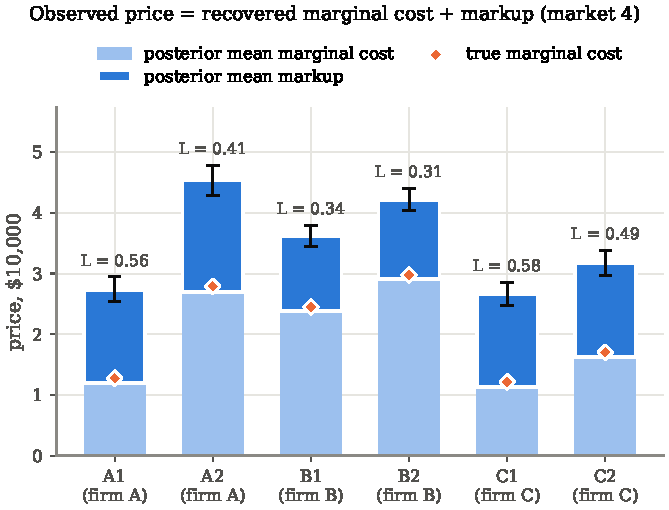
\includegraphics[width=0.85\linewidth]{chapters/blp/figures/fig_price_decomposition.pdf}
\caption{GBC posterior decomposition of observed prices into marginal cost and markup in market
4, with 90\% intervals on the markup and the true marginal costs (diamonds). The label above each
bar is the posterior mean Lerner index.}
\label{blp:fig:decomp}
\end{figure}

The GBC prior is uniform on a box: $\alpha\in[0.4,2]$, $\sigma_p\in[0,1]$,
$\sigma_x\in[0,1.5]$, $\beta_0\in[0.5,3.5]$, $\beta_1\in[0,2]$, $\beta_2\in[-0.5,1.5]$,
$\gamma_0\in[1,3]$, $\gamma_1\in[0,1]$, $\gamma_2\in[0,0.6]$, $\sigma_\xi\in[0.2,1]$,
$\sigma_\omega\in[0.1,0.6]$, $\rho\in[-0.5,0.5]$, with each conduct model equally likely. A draw is kept only if the solver converges with every price in $(0,60)$, in units of \$10{,}000, every share above $10^{-7}$ and an inside share below $0.995$ in every market (the local round below also requires the post merger equilibrium to solve). Failed draws are redrawn, parameters and shocks together, so the effective prior is the box density weighted by the probability that a draw of the shocks gives a valid equilibrium at those parameters, and the equal numbers per conduct make the three conduct models equally likely in the reference table. In that table 95 percent of the Bertrand Nash draws and 98 percent of the joint monopoly draws were kept, but only 50 percent of the perfect competition draws. Of the 2{,}948 rejected perfect competition draws, 2{,}776 had a price of zero or below and 172 an inside share of 0.995 or more; since prices equal costs under perfect competition, the effective prior for that conduct is concentrated on parameters that keep every cost positive. The other reference tables of the chapter kept 87 to 98 percent of their draws. The
amortized reference table has 3{,}000 industries per conduct model. A local second round draws
8{,}000 Bertrand Nash industries from the prior truncated to a box covering the first round
posterior and records the estimands; its posterior uses the 1{,}500 residuals nearest the fit at $S^{\mathrm{obs}}$, unweighted. We compare with logit IV, BLP GMM (two step, sandwich
standard errors, 250 Krinsky and Robb draws for derived quantities) and the Bayesian inversion MCMC of
Section~\ref{blp:sec:existing} (one chain of 5{,}000 iterations, the first 1{,}500 discarded). The seeded chain's path depends on numerical libraries: runs on other machines moved the posterior mean of $\alpha$ in its second decimal and its posterior standard deviation by less than 0.005. No comparison below turns on this Monte Carlo noise. The exogenous design $(\bm x,\bm w)$ is held fixed, so every procedure conditions on it.

Every true value and estimate in this chapter uses the 200 simulated consumers that generated the data. Holding the observed shares and prices fixed, using 3{,}200 antithetic normal draws instead moves the true merger price effect from 13.3 to 14.5 percent and the industry Lerner index from 0.434 to 0.454. The effect at the GMM estimate moves from 12.7 to 13.4 percent. These application shifts are smaller than the corresponding posterior standard deviations in Table~\ref{blp:tab:main}, but larger than its rounding. Across 50 Bertrand Nash industries drawn from the prior, the median change in the merger effect is 1.5 percentage points and the largest is 11.3. The reported results therefore describe the model with 200 consumers.

Numerical searches support the computed equilibria. The solver reaches the same prices from six starting points. Before the merger, we check all 24 firm and market pairs in the first eight markets using a 160 by 160 grid of markups from 0.01 to 40 and 60 random quasi Newton starts. No search finds a profitable deviation, and the second order condition holds at every pair, with 200, 800, 3{,}200 and 12{,}800 draws. After the merger, a separate quasi Newton search from six starts finds no profitable deviation in the 16 firm and market pairs, with 200 and 3{,}200 draws.

\subsection{Conduct, demand parameters and markups}

\paragraph{Conduct.} In the space of markup regression loadings (Figure~\ref{blp:fig:conduct}),
the three conduct models separate as Lemma~\ref{blp:lem:logit} predicts, and the observed data sit inside the Bertrand Nash cloud. The posterior probability of
Bertrand Nash is \numpbert, and on the \numncal\ held out simulated industries of Section~\ref{blp:sec:calibration} the classifier recovers the true
conduct with balanced accuracy \numconductacc. With the posterior this concentrated, the model averaging of Proposition~\ref{blp:prop:bma} changes little, here and in Section~\ref{blp:sec:misspec}, where what changes the answer is estimating conduct instead of maintaining Bertrand Nash.

\begin{figure}[htbp]
\centering
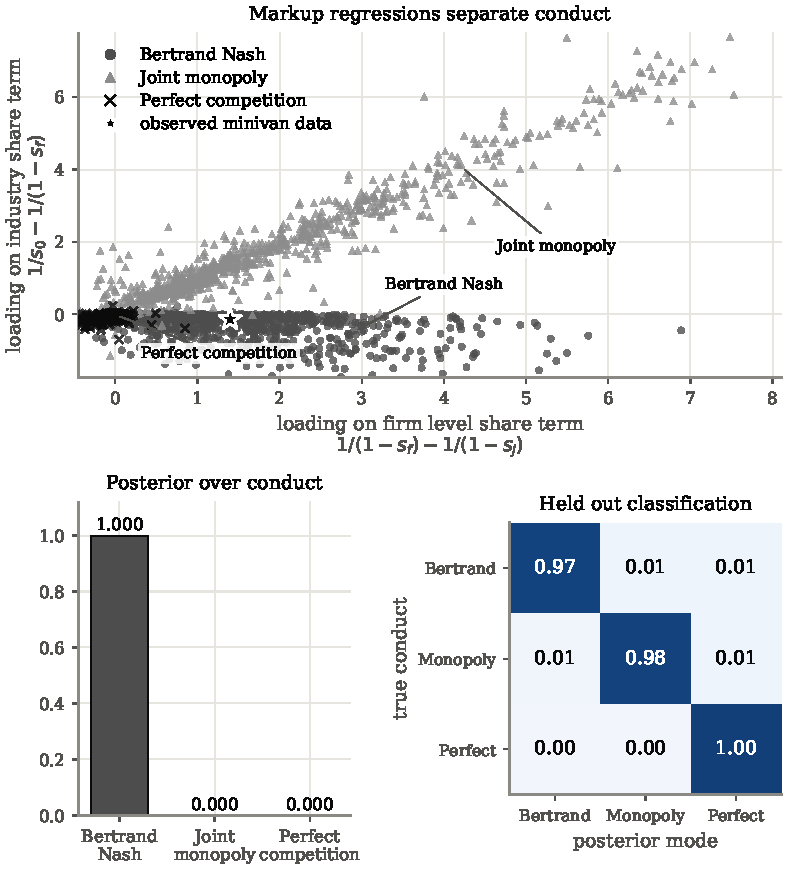
\includegraphics[width=\linewidth]{chapters/blp/figures/fig_conduct.pdf}
\caption{Top: loadings of prices on the nested markup regressors for simulated industries under
three conduct models; the star is the observed data. Bottom left: GBC posterior over conduct. Bottom right:
classification of conduct on held out simulated industries.}
\label{blp:fig:conduct}
\end{figure}

\paragraph{Demand parameters and markups.} Table~\ref{blp:tab:main} and Figure~\ref{blp:fig:theta} report the demand parameters. Logit IV fixes $\sigma_p=\sigma_x=0$, imposing independence of irrelevant alternatives\index{independence of irrelevant alternatives|textbf}; in this industry it understates price sensitivity and overstates markups. BLP GMM recovers the parameters, but its standard error for $\sigma_p$ is nearly two fifths of the estimate. The micro moments
pin $\sigma_p$ down: the GBC posterior standard deviation of $\sigma_p$ falls from
\numspnomicro\ without them to \numspmicro\ with them. The inversion MCMC, which conditions on the full data, has a posterior standard deviation for $\alpha$ of 0.050 against 0.087 for the local GBC posterior with micro moments. Part of that gap may be the price of conditioning on summaries, but the two posteriors also differ in likelihood (a reduced form for price against the equilibrium) and in prior, so the comparison does not isolate it. For $\sigma_p$ the order reverses (0.067 against 0.047) because the inversion MCMC does not use the micro moments. Figure~\ref{blp:fig:ridge} shows why markups
are about as well determined as $\alpha$ and better than $\sigma_p$: $\alpha$ and $\sigma_p$ trade off along a
ridge on which $\E[\alpha_i]$ is nearly constant, and the implied Lerner index tracks
$1/\E[\alpha_i]$ to a degree (correlation \numcorrLa). Figure~\ref{blp:fig:lerner} reports product level Lerner
indices.

\begin{table}[htbp]
\centering\footnotesize\setlength{\tabcolsep}{2.5pt}
\resizebox{\linewidth}{!}{\begin{tabular}{lcccccc}
\toprule
 & $\alpha$ & $\sigma_p$ & $\sigma_x$ & Lerner & $\Delta p/p$, \% & $\Delta$CS \\
\midrule
\csname @@input\endcsname chapters/blp/table_main.tex 
\bottomrule
\end{tabular}}
\caption{Posterior means (standard deviations) of the nonlinear demand parameters and of the
antitrust estimands obtained by plugging in parameter draws, for the Bayesian rows (GBC and the inversion MCMC). For GMM and logit the parameter columns give the point estimate and its sandwich standard error, and the derived quantities the mean (standard deviation) of Krinsky and Robb draws from the asymptotic normal approximation. $\Delta p/p$ is the
average over the four merging products; $\Delta$CS is per consumer per market in units of
\$10{,}000.}
\label{blp:tab:main}
\end{table}

\begin{figure}[htbp]
\centering
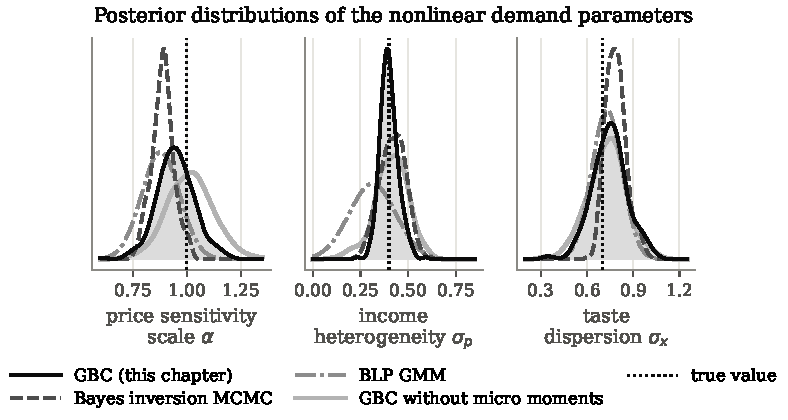
\includegraphics[width=\linewidth]{chapters/blp/figures/fig_theta_posteriors.pdf}
\caption{Posterior distributions of $\theta_2$. GMM is shown as its asymptotic normal
approximation.}
\label{blp:fig:theta}
\end{figure}

\begin{figure}[htbp]
\centering
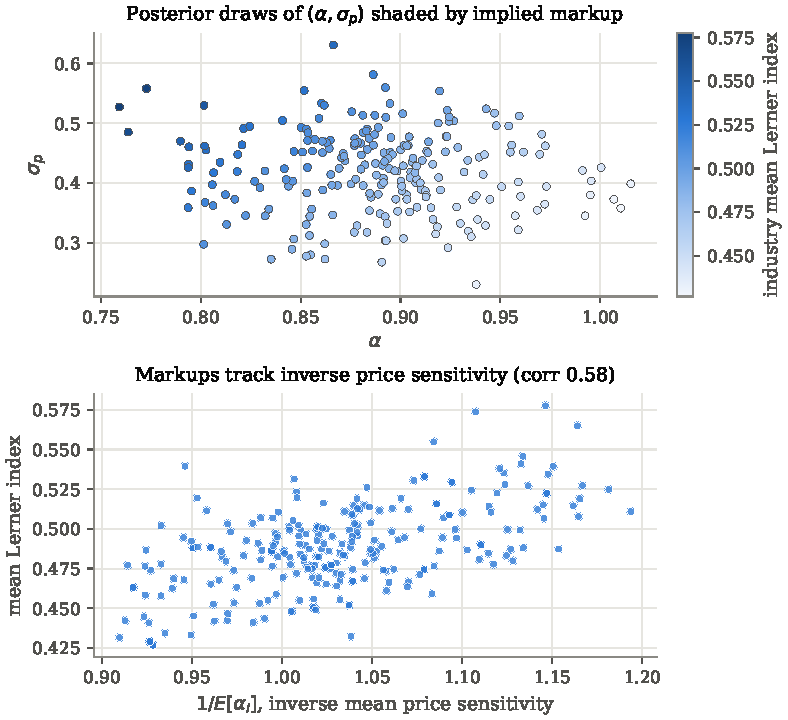
\includegraphics[width=\linewidth]{chapters/blp/figures/fig_markup_ridge.pdf}
\caption{Top: posterior draws of $(\alpha,\sigma_p)$ from the Bayesian inversion MCMC, shaded by
the industry mean Lerner index they imply. Bottom: the Lerner index against the inverse of mean
price sensitivity.}
\label{blp:fig:ridge}
\end{figure}

\begin{figure}[htbp]
\centering
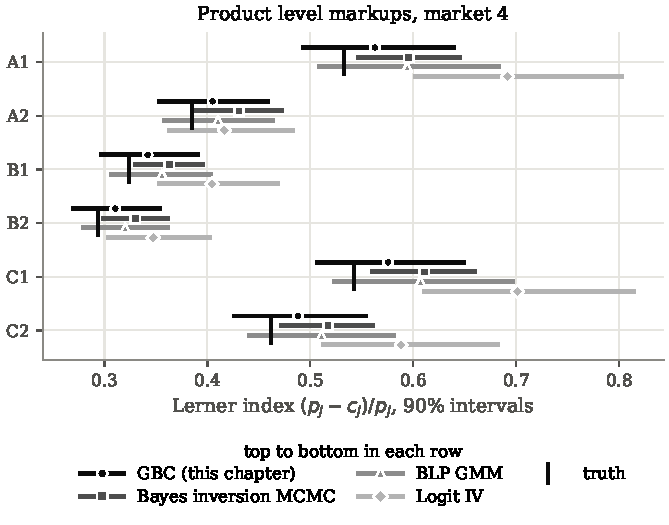
\includegraphics[width=0.85\linewidth]{chapters/blp/figures/fig_lerner_forest.pdf}
\caption{Product level Lerner indices in market 4, 90\% intervals by method, with the truth.}
\label{blp:fig:lerner}
\end{figure}

\subsection{Substitution, screens and the merger}
Figure~\ref{blp:fig:diversion} compares diversion ratios. The logit spreads diversion in proportion
to shares, $\mathrm{DR}_{jk} = s_k/(1-s_j)$, while the random coefficients posterior sends more diversion
to products with similar $x_1$, the pattern that matters when merging products are close in characteristic space. Figure~\ref{blp:fig:guppi} shows the posterior
GUPPI of each merging model; the probability of exceeding a 5\% screen is \numguppia\ for each of A1, A2, B1 and B2.

\begin{figure}[htbp]
\centering
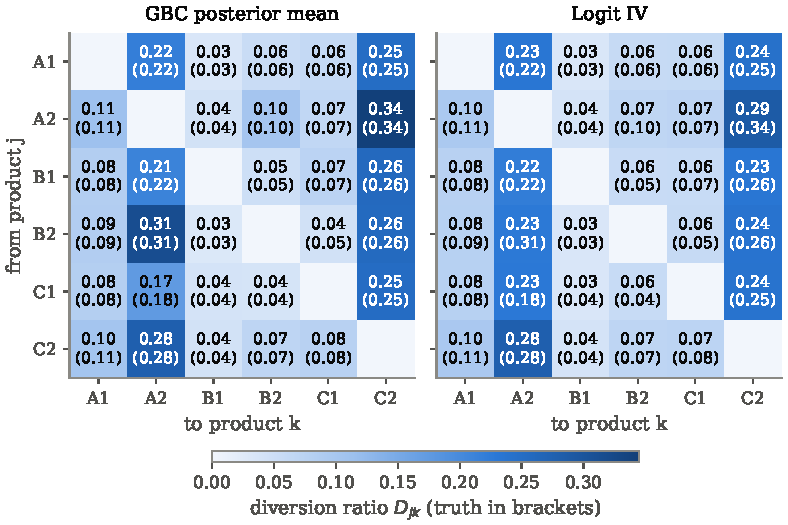
\includegraphics[width=\linewidth]{chapters/blp/figures/fig_diversion.pdf}
\caption{Diversion ratios in market 4: GBC posterior means and logit, with the truth in brackets.}
\label{blp:fig:diversion}
\end{figure}

\begin{figure}[htbp]
\centering
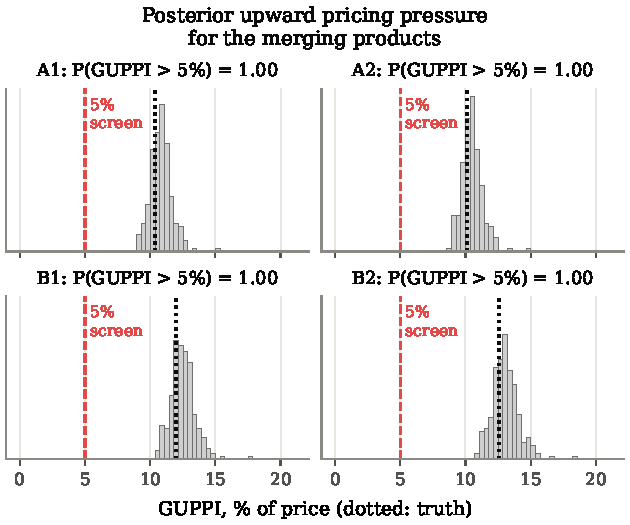
\includegraphics[width=0.8\linewidth]{chapters/blp/figures/fig_guppi.pdf}
\caption{Posterior GUPPI for the four merging products (market averages), with the truth
(dotted) and a 5\% screen.}
\label{blp:fig:guppi}
\end{figure}

Figure~\ref{blp:fig:merger} shows the merger simulation. In truth the prices of the merging models rise
by between 12\% and 15\% and those of the outsider C by 1.5\%, the strategic complement response;
the GBC posterior means are within about half a percentage point of each. Logit IV reports a merging
party price increase of \numdplogit\% against a true \numdptrue\%. The direct GBC estimand posterior (Figure~\ref{blp:fig:estimands}) gives a merging party price increase of $\numdpdir\%$
(s.d. \numdpdirsd), an industry Lerner index of $\numldir$ (s.d. \numldirsd) and a consumer
surplus change of $\numcsdir$ (s.d. \numcsdirsd), against true values of $\numdptrue\%$,
$\numltrue$ and $\numcstrue$.

\begin{figure}[htbp]
\centering
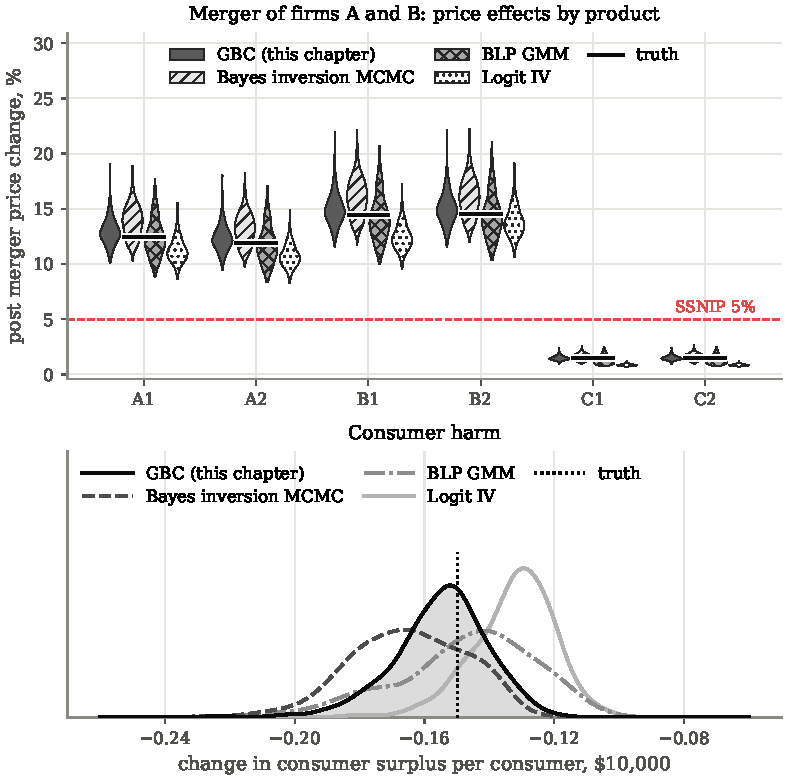
\includegraphics[width=\linewidth]{chapters/blp/figures/fig_merger.pdf}
\caption{Merger of manufacturers A and B. Top: price changes by product, averaged
over markets, from posterior draws (GBC, Bayes inversion MCMC) and Krinsky and Robb draws (BLP GMM, logit IV). Bottom: the same draws for the change in consumer surplus per consumer.}
\label{blp:fig:merger}
\end{figure}

\begin{figure}[htbp]
\centering
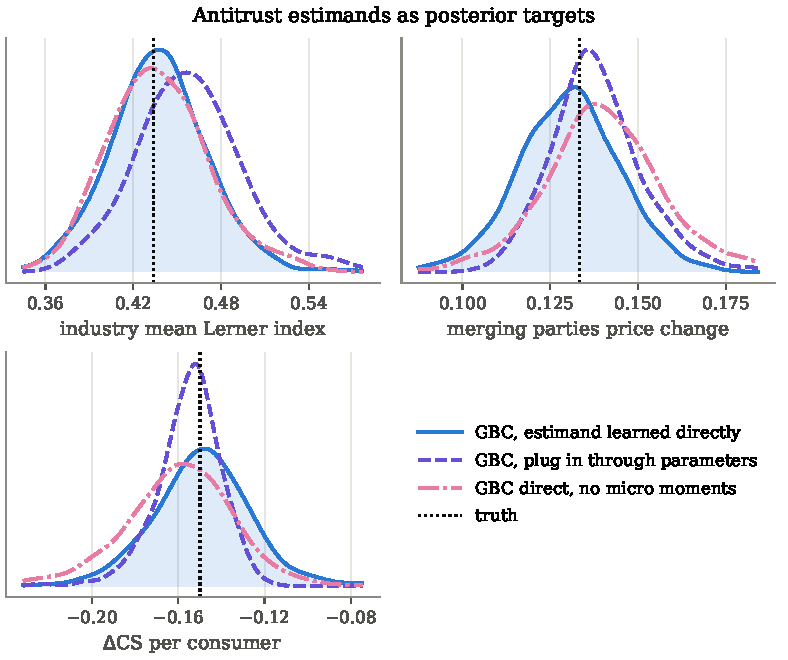
\includegraphics[width=\linewidth]{chapters/blp/figures/fig_estimands.pdf}
\caption{Antitrust estimands learned directly by GBC, compared with plugging GBC parameter draws
into Propositions \ref{blp:prop:markup} and \ref{blp:prop:merger}, and with the direct estimand learned
without micro moments.}
\label{blp:fig:estimands}
\end{figure}

\subsection{The decision}
Every method puts essentially all its mass, posterior or Krinsky and Robb, above the 5\% threshold and so reaches the same decision to challenge. Remedies and divestiture sizing, however, turn on the size of the effect. Figure~\ref{blp:fig:decision} plots $\Prob(\Delta p/p > r\mid\text{data})$ against $r$,
the input to Proposition~\ref{blp:prop:decision}. The GBC curve is the posterior of the estimand learned directly as a target, while the GBC rows of Table~\ref{blp:tab:main} plug in parameter draws. At $r = 12\%$ the GBC probability is
\numpgbcxii{} against \numplogitxii{} for logit IV; at $r=15\%$ it is \numpgbcxv{} against
\numplogitxv. By understating substitution between close products, logit understates the probability of large harm.

The curve in Figure~\ref{blp:fig:decision} is the whole output of the analysis as far as the decision is concerned. Read it at the harm threshold $r$ and compare its height with $\ell_1/(\ell_1+\ell_2)$, the cost of a wrongful challenge divided by the sum of the two error costs\index{merger!losses from wrongful challenge and clearance|textbf} (Proposition~\ref{blp:prop:decision}). A court that weighs the two errors equally compares it with $0.5$, an agency that regards underenforcement as nine times as costly with $0.1$, and both use the same curve. A confidence interval for $\Delta p/p$ supports none of this directly, because it fixes the error probability in advance and reports a set, whereas the agency wants to fix the set, the harmful region above $r$, and learn the probability.



\begin{figure}[htbp]
\centering
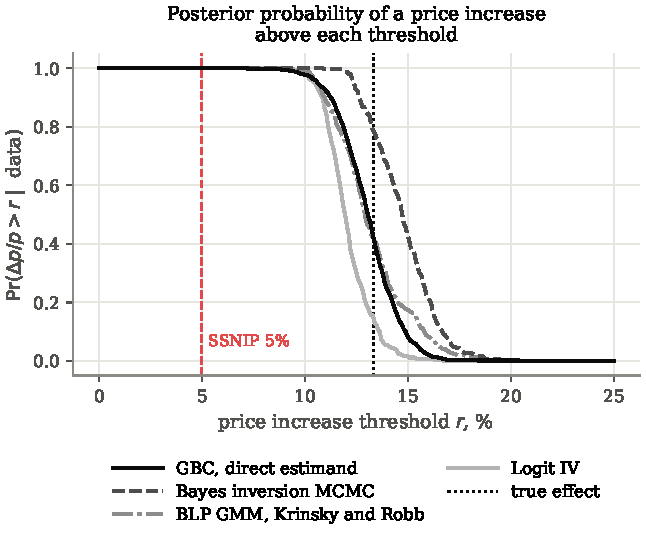
\includegraphics[width=0.82\linewidth]{chapters/blp/figures/fig_decision.pdf}
\caption{Probability that the merging parties' average price increase exceeds
$r$: the posterior for GBC and for the Bayesian inversion MCMC, and Krinsky and Robb draws for BLP GMM and logit IV. It is the input to the Bayes rule of Proposition~\ref{blp:prop:decision}.}
\label{blp:fig:decision}
\end{figure}

\section[A cereal merger and its remedy]{An antitrust case: a cereal merger with a divestiture remedy}\label{blp:sec:cereal}

Merger review rarely ends with a yes or no on the merger as proposed: the parties offer remedies\index{merger!remedy|textbf}, typically divestitures, and the agency must decide whether they restore competition. This case is patterned on ready to eat cereal\index{merger!cereal example with a divestiture|textbf} (Nevo 2000).

Eight brands are sold by four firms: a leader A with
three brands, B and C with two each, and a fringe firm D with one, observed in $T=30$ city markets.
Inside shares are \numcershA\% for A, \numcershB\% for B, \numcershC\% for C and \numcershD\% for D, so inside goods hold \numcerinside\% of the market. Demand and costs follow Section~\ref{blp:sec:model}, with the parameters of Section~\ref{blp:sec:app} except the demand intercept, $\beta_0 = 1.2$ rather than 2, and Bertrand Nash pricing.

Firms B and C, the second and third largest, propose to merge. The agency considers divesting C2 to the fringe firm D and asks whether it brings the price effect below 5\%.

GBC is trained once on 6{,}000 simulated Bertrand Nash industries at this
design, with five estimands as targets: the industry Lerner index, and the average price effect over the merging parties' four brands B1, B2, C1 and C2 (C2 included after it is divested) and the consumer surplus change per consumer, each with and without the remedy. Each is computed exactly in every simulated industry from the two post merger equilibria (Proposition~\ref{blp:prop:merger} with $H^{\mathrm{post}}$ set by the merger or by the
remedied ownership). Parameters are drawn from the prior of Section~\ref{blp:sec:app}, the two micro moments enter the summaries with their survey noise, and the posterior uses the 1{,}500 residuals nearest the fit at the observed summaries. BLP GMM is fitted to the same data, with estimands from plugging in $\hat\theta_2$ and 150 Krinsky and Robb draws for uncertainty.

\begin{table}[htbp]
\centering\small
\resizebox{\linewidth}{!}{\begin{tabular}{lcc}
\toprule
 & Merger & Merger with divestiture of C2 \\
\midrule
Truth & \numcerdpmtrue\% & \numcerdprtrue\% \\
GBC posterior mean (s.d.) & \numcerdpmgbc\% (\numcerdpmgbcsd) & \numcerdprgbc\% (\numcerdprgbcsd) \\
BLP GMM (Krinsky and Robb s.d.) & \numcerdpmgmm\% (\numcerdpmgmmsd) & \numcerdprgmm\% (\numcerdprgmmsd) \\
Logit IV & \numcerdpmlogit\% & \numcerdprlogit\% \\
\midrule
GBC $\Prob(\Delta p/p > 5\%\mid\data)$ & \numcerpmgbc & \numcerprgbc \\
GMM $\Prob(\Delta p/p > 5\%)$, Krinsky and Robb & \numcerpmgmm & \numcerprgmm \\
\midrule
True $\Delta$CS per consumer & $\numcercsmtrue$ & $\numcercsrtrue$ \\
GBC posterior mean $\Delta$CS & $\numcercsmgbc$ & $\numcercsrgbc$ \\
\bottomrule
\end{tabular}}
\caption{The cereal case: merging parties' average price effect and consumer surplus change, with
and without the remedy.}
\label{blp:tab:cereal}
\end{table}

\begin{figure}[htbp]
\centering
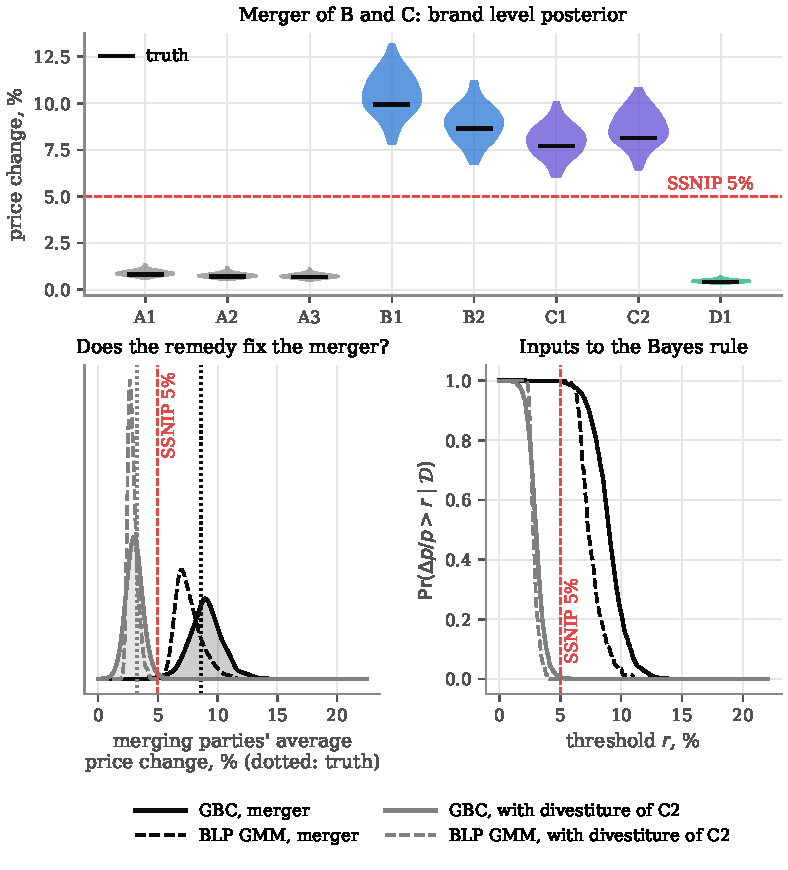
\includegraphics[width=\linewidth]{chapters/blp/figures/fig_cereal.pdf}
\caption{The cereal case. Top: GBC posterior of brand level price effects of the B and C merger.
Bottom left: posterior of the merging parties' average price effect with and without the divestiture,
GBC (solid) and BLP GMM (dashed); black is the merger as proposed and gray the remedy, here and in the bottom right panel. Bottom right: $\Prob(\Delta p/p>r\mid\data)$, the input to
Proposition~\ref{blp:prop:decision}.}
\label{blp:fig:cereal}
\end{figure}

Table~\ref{blp:tab:cereal} and Figure~\ref{blp:fig:cereal} report three findings.
\begin{enumerate}
\item The true average price effect on the merging brands is \numcerdpmtrue\%. GBC
reports \numcerdpmgbc\% with posterior standard deviation \numcerdpmgbcsd; BLP GMM reports
\numcerdpmgmm\% and logit \numcerdpmlogit\%. Both understate the effect in this industry. Logit fixes diversion in proportion to shares by independence of irrelevant alternatives\index{independence of irrelevant alternatives}, which need not match the substitution between the merging brands, so the sign of its error is a finding here and not a consequence of the model. B1 and B2 rise most because their partner C has the larger share (\numcershC\% against \numcershB\%), as Lemma~\ref{blp:lem:pressure} predicts under logit, where markup pressure on $f$ is increasing in $s_n$; with random coefficients the lemma is an approximation.
\item Divesting C2 removes about half the partner's share and, by
Lemma~\ref{blp:lem:pressure}, more than half of the markup pressure on B. The true effect falls to
\numcerdprtrue\%. GBC gives \numcerdprgbc\% (s.d. \numcerdprgbcsd) and BLP GMM \numcerdprgmm\% with a
Krinsky and Robb standard deviation of \numcerdprgmmsd. The posterior standard deviation is three times larger, but a few extreme draws inflate it (item 3), and the true remedied effect lies within 1.645 Krinsky and Robb standard deviations of the GMM estimate, so on this data set the narrower GMM band is not shown to be overconfident.
\item With equal error costs, $\ell_1 = \ell_2$, Proposition~\ref{blp:prop:decision} challenges
when $\Prob(\Delta p/p > 5\%\mid\data) > 0.5$. GBC gives \numcerpmgbc{} for the merger and
\numcerprgbc{} with the remedy, so the Bayes rule challenges the merger as proposed and accepts the
remedy. The entry for the remedy is a count of posterior draws, \numcerprgbcnabove{} of \numcerngbcdraws{} above 5 percent. A normal curve with the mean and standard deviation of the table would give 0.06, but a few extreme draws inflate that standard deviation: 90 percent of the draws lie between \numcerdprgbcqlo{} and \numcerdprgbcqhi{} percent. An agency weighing underenforcement more heavily, say $\ell_2 = 9\ell_1$, challenges whenever the probability exceeds $0.1$ and still accepts the remedy. The GMM probabilities lead to the same actions here, but with an understated merger effect; the consumer surplus loss the remedy avoids, $\numcercsrgbc - (\numcercsmgbc) = 0.039$ per
consumer under GBC, is what sizes the divestiture.
\end{enumerate}

\section[Repeated sampling]{Repeated sampling: GBC against BLP GMM}\label{blp:sec:mc}

One data set cannot separate method from luck, so we redraw the
unobservables $(\bm\xi,\bm\omega)$ and the micro survey noise \nummcnxv{} times with the design and
the true parameters fixed, at $T=40$ and at $T=15$ markets\index{simulation study!repeated sampling, GBC against BLP GMM|textbf}. In each
replication we fit BLP GMM\index{BLP GMM!against generative Bayesian computation|textbf} (three starting values, two step, sandwich covariance, 100 Krinsky and
Robb draws pushed through Propositions \ref{blp:prop:markup} and \ref{blp:prop:merger}; the GMM point
estimate of an estimand is the median of these draws, and Table~\ref{blp:tab:mcplug} adds the plug in $g(\hat\theta_2)$) and the amortized GBC posterior, trained once per design on 6{,}000 Bertrand
Nash industries drawn from the prior, and its posterior uses the 1{,}500 residuals nearest the fit at the summaries of the replication, unweighted. The amortized posterior is less sharp than the local second round on the data set of Section~\ref{blp:sec:app}, so this comparison is probably conservative for GBC, although we did not run the local round in repeated sampling.

Table~\ref{blp:tab:mc} and Figures \ref{blp:fig:mcerr} and \ref{blp:fig:mccov} report bias, root mean
squared error, coverage of nominal 90\% intervals and median interval length, and Table~\ref{blp:tab:mcse} their Monte Carlo standard errors. Six findings
follow.

\begin{enumerate}
\item The root mean squared error of the merger price effect, in percentage points, is \nummcdprmsegbcxl{} for GBC against \nummcdprmseplugxl{} for the GMM plug in $g(\hat\theta_2)$ at $T=40$, and \nummcdprmsegbcxv{} against \nummcdprmseplugxv{} at $T=15$ (Table~\ref{blp:tab:mcplug}). GBC has the larger absolute bias (Table~\ref{blp:tab:mc}, against \nummcdpbiasplugxl{} and \nummcdpbiasplugxv{} for the plug in) and the smaller variance. Taking the median of the Krinsky and Robb draws as the GMM estimate, as Table~\ref{blp:tab:mc} does, raises its error to \nummcdprmsegmmxl{} at $T=40$ and \nummcdprmsegmmxv{} at $T=15$, the latter with Monte Carlo standard error \nummcdprmsesegmmxv{} and driven by the replications of item 2 whose draws explode. GMM is nearly unbiased for $\alpha$; its weakness is the variance parameter and everything downstream. Root
mean squared error for $\sigma_p$ is \nummcsprmsegbcxl{} for GBC against \nummcsprmsegmmxl{} for
GMM at $T=40$, and \nummcsprmsegbcxv{} against \nummcsprmsegmmxv{} at $T=15$.
\item The GMM estimate of $\sigma_p$ is below $0.05$ in \nummcboundxv{} of
\nummcnxv{} replications at $T=15$ (\nummcboundxl{} at $T=40$). In \nummcexplxv{} replications at
$T=15$ the Krinsky and Robb distribution of the merger effect has its 95th percentile above
100\%, because a normal approximation near the boundary puts mass on large $\sigma_p$ and
hence on consumers with almost no price sensitivity. 
\item GBC intervals are conservative, covering at 0.95 to 1.00, while
GMM intervals for the Lerner index cover at \nummclercovgmmxl{} at $T=40$ and \nummclercovgmmxv{} at $T=15$, with Monte Carlo standard errors \nummclercovsegmmxl{} and \nummclercovsegmmxv{}. That is 2.5 and 7 Monte Carlo standard errors below 0.90, so the undercoverage is clear at $T=15$ and likely at $T=40$. GBC intervals for $\sigma_p$ are about half
as long as GMM's (\nummcsplengbcxl{} against \nummcsplengmmxl{} at $T=40$); for the merger effect
the lengths are similar.
\item Part of the GBC advantage comes from the micro moments, which aggregate BLP does not use; removing them raises its root mean squared error for $\sigma_p$ to
\nummcsprmsenmxl{} ($T=40$) and \nummcsprmsenmxv{} ($T=15$), and for the merger effect to
\nummcdprmsenmxl{} and \nummcdprmsenmxv{}, still below GMM in every case, although at $T=40$ the gap for $\sigma_p$ is about three Monte Carlo standard errors and the GMM plug in for the merger effect (\nummcdprmseplugxl{}) comes close.
\item With $T=15$ the amortized GBC posterior for the industry Lerner index
is pulled towards the prior (bias 0.12), with wide intervals. The network was trained over the whole prior; the local second round of Section~\ref{blp:sec:app} should reduce this, at the cost of a second simulation round per data set, but we ran it only on the $T=40$ application.
\item With a true $\sigma_p$ of 0.05, near the boundary, and the rest of the design unchanged (\nummcfivexln{} replications at $T=40$, \nummcfivexvn{} usable at $T=15$), the GMM estimate of $\sigma_p$ is below $0.05$ in \nummcfivexlbound{} and \nummcfivexvbound{} of them, and its Wald intervals for $\sigma_p$ cover at \nummcfivespcovgmmxl{} and \nummcfivespcovgmmxv{}. The Krinsky and Robb intervals for the merger price effect cover at only \nummcfivedpcovgmmxl{} and \nummcfivedpcovgmmxv{}, and the median of the draws has root mean squared error \nummcfivedprmsegmmxl{} and \nummcfivedprmsegmmxv{} percentage points, against \nummcfivedprmsegbcxl{} and \nummcfivedprmsegbcxv{} for GBC, whose intervals cover at \nummcfivedpcovgbcxl{} and \nummcfivedpcovgbcxv{}. We did not compute the plug in for this design.
\end{enumerate}


\begin{table}[htbp]
\centering\footnotesize\setlength{\tabcolsep}{5pt}
\begin{tabular}{lcccccccc}
\toprule
 & \multicolumn{4}{c}{BLP GMM} & \multicolumn{4}{c}{GBC} \\
\cmidrule(lr){2-5}\cmidrule(lr){6-9}
 & bias & RMSE & cover & length & bias & RMSE & cover & length \\
\midrule
\csname @@input\endcsname chapters/blp/table_mc.tex 
\bottomrule
\end{tabular}
\caption{Repeated sampling performance. Coverage and length refer to nominal 90\% intervals:
Wald for GMM parameters, Krinsky and Robb for GMM estimands, posterior quantiles for GBC. The
truth of the estimands varies across replications with $(\bm\xi,\bm\omega)$ and is computed
exactly in each.}
\label{blp:tab:mc}
\end{table}

\begin{figure}[htbp]
\centering
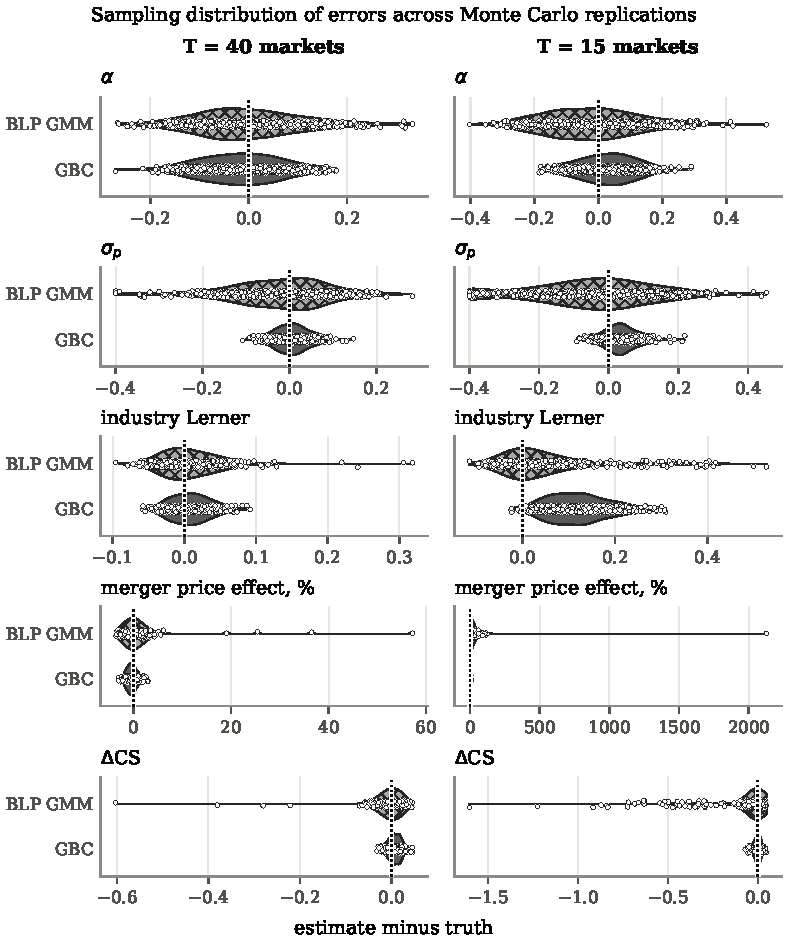
\includegraphics[width=\linewidth]{chapters/blp/figures/fig_mc_errors.pdf}
\caption{Errors across Monte Carlo replications, BLP GMM point estimates against GBC posterior
means, with $T=40$ (left) and $T=15$ (right) markets.}
\label{blp:fig:mcerr}
\end{figure}

\begin{figure}[htbp]
\centering
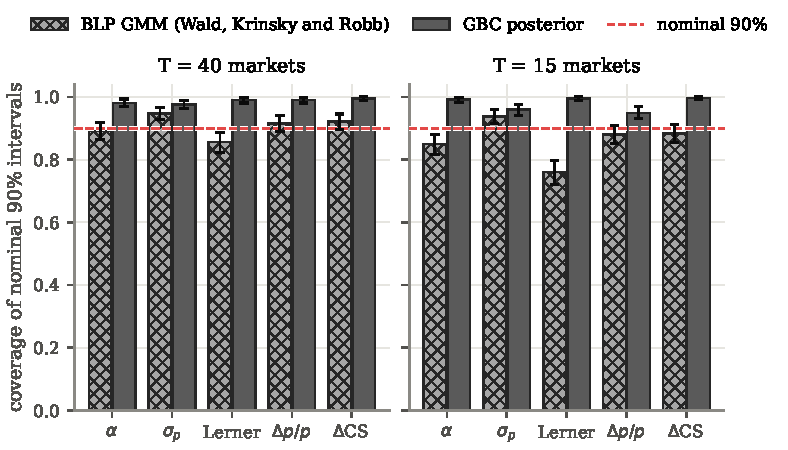
\includegraphics[width=\linewidth]{chapters/blp/figures/fig_mc_coverage.pdf}
\caption{Coverage of nominal 90\% intervals across Monte Carlo replications.}
\label{blp:fig:mccov}
\end{figure}

\begin{table}[htbp]
\centering\footnotesize\setlength{\tabcolsep}{5pt}
\begin{tabular}{lcccc}
\toprule
 & \multicolumn{2}{c}{Median of Krinsky and Robb draws} & \multicolumn{2}{c}{Plug in $g(\hat\theta_2)$} \\
\cmidrule(lr){2-3}\cmidrule(lr){4-5}
 & bias & RMSE & bias & RMSE \\
\midrule
\csname @@input\endcsname chapters/blp/table_mc_plug.tex 
\bottomrule
\end{tabular}
\caption{Two GMM point estimates of the estimands in the design of Table~\ref{blp:tab:mc} (true $\sigma_p=0.4$, 500 replications at each $T$): the median of the 100 Krinsky and Robb draws, as in that table, and the plug in of the GMM estimate $\hat\theta_2$.}
\label{blp:tab:mcplug}
\end{table}

\begin{table}[htbp]
\centering\footnotesize\setlength{\tabcolsep}{5pt}
\begin{tabular}{lcccccccc}
\toprule
 & \multicolumn{4}{c}{BLP GMM} & \multicolumn{4}{c}{GBC} \\
\cmidrule(lr){2-5}\cmidrule(lr){6-9}
 & bias & RMSE & cover & length & bias & RMSE & cover & length \\
\midrule
\csname @@input\endcsname chapters/blp/table_mc_se.tex 
\bottomrule
\end{tabular}
\caption{Monte Carlo standard errors of the entries of Table~\ref{blp:tab:mc}, from 500 replications: for a bias, the standard deviation of the error over $\sqrt{500}$; for a root mean squared error, the standard deviation of the squared error over twice the root mean squared error times $\sqrt{500}$; for a coverage $c$, $\sqrt{c(1-c)/500}$. Interval lengths are medians and carry no standard error here.}
\label{blp:tab:mcse}
\end{table}

\section{Calibration on fresh industries}\label{blp:sec:calibration}

Intervals used in litigation should mean what they say across the industries a procedure might face, not only at one true parameter. Because the GBC posterior is amortized, we check this on \numncal\ fresh industries\index{calibration!on fresh industries|textbf} drawn from the prior under all three conduct models (the draws, of 450, that produced a valid equilibrium), each needing one simulation and one network evaluation; the intervals are those of the posterior given the true conduct, so conduct uncertainty is not part of this check. Figure~\ref{blp:fig:calibration}
reports coverage of nominal 90\% intervals for all twelve parameters. With in sample residuals the
average coverage is \numcovnaive; with cross fitted residuals it is \numcovavg, slightly conservative and never below
\numcovmin, and the probability integral transforms are roughly flat, with too little mass in the outer bins for $\alpha$, as slightly conservative intervals imply. The cross fitted intervals are slightly too wide because an out of fold residual carries the error of its fold network on top of the noise, while the prediction at $S^{\mathrm{obs}}$ averages the three fold networks and so carries less of that error.



The probabilities a hearing turns on can be checked the same way. On the \numncal\ fresh industries, the conduct classifier has Brier score 0.031, against 0.667 for equal probabilities. This score is the squared distance between the vector of conduct probabilities and the indicator vector for the true conduct, averaged over industries. The most probable conduct is correct in 98 percent of industries. Pooling the three probabilities per industry gives 1{,}062 values; only 17 lie between 0.1 and 0.9, too few to assess calibration in that range.

For the merger, whose effect the calibration industries do not record, we held out 1{,}000 industries of each Bertrand Nash reference table of Section~\ref{blp:sec:mc} ($T=40$ and $T=15$) and trained on the other 5{,}000. Table~\ref{blp:tab:calprob} compares posterior and base rate Brier scores and reports the calibration gap. The posterior's Brier score is 3 to 6 times smaller than the base rate's, and no gap exceeds 0.025. This check holds conduct fixed at Bertrand Nash.

\begin{table}[htbp]
\centering\footnotesize\setlength{\tabcolsep}{5pt}
\begin{tabular}{ccccc}
\toprule
$T$ & threshold $r$ (\%) & Brier, GBC & Brier, base rate & calibration gap \\
\midrule
40 & 5  & 0.016 & 0.062 & 0.009 \\
   & 12 & 0.042 & 0.220 & 0.019 \\
   & 15 & 0.039 & 0.249 & 0.013 \\
\midrule
15 & 5  & 0.025 & 0.083 & 0.015 \\
   & 12 & 0.060 & 0.244 & 0.025 \\
   & 15 & 0.063 & 0.245 & 0.019 \\
\bottomrule
\end{tabular}
\caption{Calibration of the GBC posterior probability that the merging parties' price effect exceeds $r$, on 1{,}000 held out Bertrand Nash industries at each $T$, with the network trained on the other 5{,}000. The Brier score is the mean squared difference between the predicted probability and the event indicator; the base rate predicts the observed frequency in the held out industries. The calibration gap is the mean absolute difference between predicted and observed frequencies over ten groups of 100 industries ordered by predicted probability.}
\label{blp:tab:calprob}
\end{table}

Calibration\index{calibration} over the prior does not guarantee calibration at any particular true parameter: at one such parameter, the Monte Carlo at $T=15$ shows the amortized Lerner posterior pulled towards the prior. And fresh industries come from the same demand and cost model that generated the training table, so this is a check on the computation, not on the economics; Section~\ref{blp:sec:misspec} checks the economics, as far as conduct goes.

\begin{figure}[htbp]
\centering
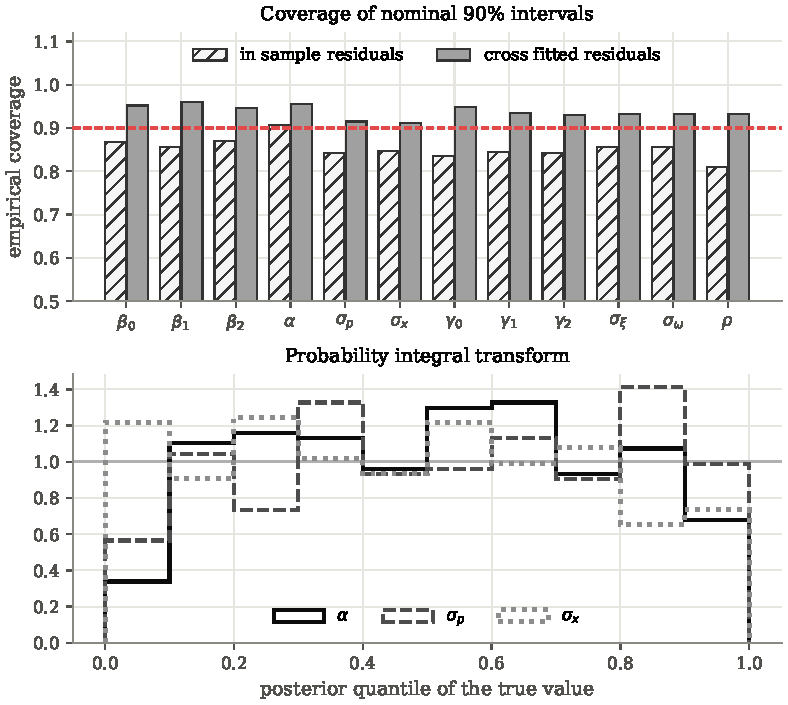
\includegraphics[width=\linewidth]{chapters/blp/figures/fig_calibration.pdf}
\caption{Calibration of GBC on held out industries, with the posterior given the true conduct. Top: coverage of nominal 90\% intervals with
in sample and with cross fitted residuals. Bottom: probability integral transform of the true
$\alpha$, $\sigma_p$ and $\sigma_x$ under the cross fitted posterior.}
\label{blp:fig:calibration}
\end{figure}

\section{When conduct is wrong}\label{blp:sec:misspec}

The experiment that matters most for policy generates one data set from the design of Section~\ref{blp:sec:app} under joint monopoly, and another under perfect competition, and asks each method to evaluate the A and B merger\index{conduct!wrong, misspecified|textbf}. BLP GMM, as is standard, estimates demand, then recovers costs and simulates the merger under Bertrand Nash at its point estimate, without Krinsky and Robb draws; GBC estimates conduct and uses 150 posterior draws.

\begin{itemize}
\item Collusive data\index{collusion|textbf}. A merger of two firms that already maximize joint profit changes nothing,
so the true price effect is \nummscollusiontrue\%. BLP GMM estimates demand well ($\hat\alpha = \nummscollusionalpha$) but, with Bertrand
supply, predicts \nummscollusiongmm\%, and recovers an industry Lerner index of \nummscollusionlgmm{} against a true
\nummscollusionltrue. GBC assigns posterior probability \nummscollusionpc{} to joint monopoly,
predicts \nummscollusiongbc\% and a Lerner index of \nummscollusionlgbc.
\item Competitive data. Prices equal costs and the true merger effect is \nummsperfecttrue\%.
BLP GMM again estimates demand well ($\hat\alpha = \nummsperfectalpha$) but Bertrand supply invents markups (Lerner \nummsperfectlgmm{} against
\nummsperfectltrue) and predicts \nummsperfectgmm\%. GBC assigns posterior probability
\nummsperfectpc{} to perfect competition and predicts \nummsperfectgbc\%.
\end{itemize}

Figure~\ref{blp:fig:misspec} summarizes. GMM's demand estimates are fine in both cases; the error comes entirely from the maintained supply side, which by Proposition~\ref{blp:prop:markup} determines costs and hence the counterfactual.

Estimating conduct helps only when the true conduct is among those in the reference table. In \nummspartn{} industries generated with the design of Section~\ref{blp:sec:app} and $T=40$ under partial internalization, each firm maximizing its own profit plus half of each rival's, a conduct outside the training set, the true merger price effect averages \nummsparttruedp\%. GBC puts on average probability \nummspartpcbert{} on Bertrand Nash and \nummspartpccoll{} on joint monopoly, and overstates the effect by \nummspartgbcbiasdp{} percentage points, about as much as BLP GMM with Bertrand Nash maintained (\nummspartgmmbiasdp{}; Monte Carlo standard errors \nummspartgbcsedp{} and \nummspartgmmsedp{}). Its posterior gives no sign that conduct is wrong.

\begin{figure}[htbp]
\centering
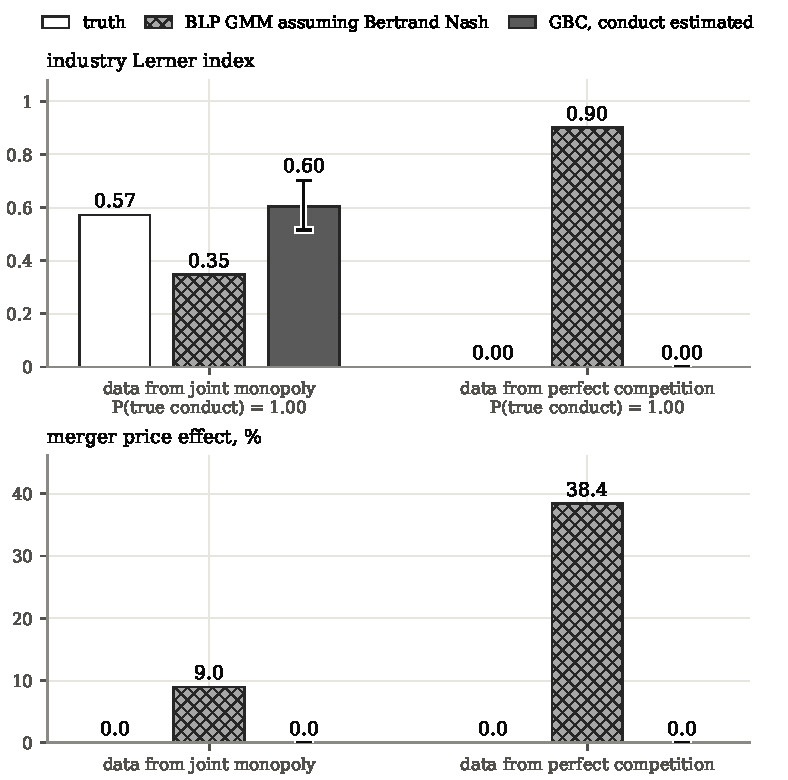
\includegraphics[width=\linewidth]{chapters/blp/figures/fig_misspec.pdf}
\caption{Merger evaluation when the data are generated by joint monopoly or by perfect
competition. BLP GMM maintains Bertrand Nash; GBC estimates conduct. Bars show the industry
Lerner index and the merging parties' price effect, with GBC 90\% intervals.}
\label{blp:fig:misspec}
\end{figure}

\section{Discussion}



The uncertainty that matters most is often structural: in Section~\ref{blp:sec:misspec} wrong conduct costs far more than sampling error in demand, and maintaining one conduct leaves this uncertainty out. A posterior over conduct is conditional on its candidate set. Duarte and coauthors (2024) give an example in which separate instrument sets favour different incorrect models, which reveals the misspecification without identifying the omitted true conduct.

Continuous conduct, such as conjectural variations or common ownership\index{common ownership|textbf} weights $H_{jk} = \kappa$ for rival products (Backus, Conlon and Sinkinson 2021), is one more coordinate of $\theta$ in Algorithm~\ref{blp:alg:gbc} (Exercise~\ref{blp:ex:kappa}). Merger efficiencies become a prior on the post merger change in $\bm c_t$, a controlled relaxation of modularity. Retrospective studies of past mergers can update the posterior for conduct and efficiencies.

\medskip\noindent\textit{Code.}\enspace The merger code and saved reference outputs are in \texttt{blp\_merger} (Appendix~\ref{app:code}).

\section{In practice}

\paragraph{The target.} The merger effect $\Delta\bm p_t$ is the intervention $\mathrm{do}(H := H^{\mathrm{post}})$ pushed through the equilibrium, and under modularity it is a function of $(\theta_2,H)$ and the data alone (Proposition~\ref{blp:prop:ident}). The decision input $\Prob(\Delta p/p > r\mid\data)$ is the fraction of posterior draws above $r$.

\paragraph{What the analyst does differently.} State the conduct models before estimating demand and report $\Prob(H\mid\data)$ rather than maintaining Bertrand Nash; in the collusive data the posterior of \nummscollusionpc{} on joint monopoly saves the decision. Fit the estimands as targets, so the merger effect is never a plug in through $\hat\theta_2$ (Proposition~\ref{blp:prop:pushforward}). Check calibration before use with cross fitted residuals (Section~\ref{blp:sec:calibration}). Report the curve $\Prob(\Delta p/p > r\mid\data)$ against $r$ rather than a point estimate with an interval, since the agency's loss ratio sets where it is read (Proposition~\ref{blp:prop:decision}). When markets are few, consider a local second round: the amortized posterior is pulled towards the prior at $T=15$, although we ran the second round only at $T=40$.

\paragraph{Against DML.} BLP GMM is already an orthogonal moment estimator: $\beta$ is profiled out and the concentrated criterion is insensitive to it at first order (Section~\ref{blp:sec:dml}, Exercise~\ref{blp:ex:dml}). A DML style treatment with cross fitted nuisances and an orthogonal score for $\theta_2$ inherits the same four limits: a fixed point target whose curvature bias orthogonality does not remove, moments flat in the random coefficient scales at zero (Proposition~\ref{blp:prop:flat}), a discrete conduct nuisance no score averages over, and an interval where a probability is needed. The evidence for BLP GMM is Section~\ref{blp:sec:mc}: root mean squared error for the merger effect in percentage points, GBC on the same aggregate data against GMM, of \nummcdprmsenmxl{} against \nummcdprmsegmmxl{} at $T=40$ (a gap of about 2.4 Monte Carlo standard errors) and \nummcdprmsenmxv{} against \nummcdprmsegmmxv{} at $T=15$, where Krinsky and Robb draws explode (\nummcdprmseplugxl{} and \nummcdprmseplugxv{} for the GMM plug in, which avoids the explosion); and the collusive data, where maintained Bertrand predicts \nummscollusiongmm\% for a true effect of \nummscollusiontrue\%. GMM is adequate with many markets, strong instruments, interior parameters and known conduct, where the two agree to first order and one optimization is cheaper than a reference table of thousands of industries.

\section{Notes and further reading}

Conlon and Gortmaker (2020) describe current BLP practice.
Merger simulation with differentiated products dates to Hausman, Leonard and Zona (1994) and
Werden and Froeb (1994), with Nevo (2000) an influential application; upward pricing
pressure is due to Farrell and Shapiro (2010); Miller and Weinberg (2017) combine conduct and
merger analysis in a modern case. Weinberg (2008) surveys retrospectives; Ashenfelter and Hosken (2010) is an example.

On the Bayesian side, Jiang, Manchanda and Rossi (2009) introduced the inversion likelihood, our benchmark, and
Gron, Polson and Viard (2003) and Viard, Gron and Polson (2015) the full equilibrium likelihood, with
equilibrium computation in Viard, Polson and Gron (2001). Generative Bayesian computation for causal problems is developed in
Nareklishvili, Polson and Sokolov (2023a); its regression adjustment ancestor is Beaumont, Zhang and Balding (2002), and the
asymptotics of summary based posteriors are in Frazier and coauthors (2018). The noise outsourcing lemma
is in Kallenberg (2002). 

\begin{exercises}
\item\label{ex:chapter_blp:1}\label{blp:ex:logit} Verify Lemma~\ref{blp:lem:logit} for a firm with products of different prices by solving the first order conditions, then show that under joint monopoly all markups equal $1/(\alpha s_0)$, and explain why the markup of a product does not depend on its own price, once shares are given, under multiproduct logit pricing.

\item\label{ex:chapter_blp:2}\label{blp:ex:outside} Suppose there is no outside good, so $s_{i0}=0$ for every consumer.
Show that the rows of $D_p^\top$ sum to zero, that $H^M\odot D_p^\top$ is singular, and hence that
joint monopoly markups are not defined. Interpret the result economically, and explain which step
of the proof of Lemma~\ref{blp:lem:dd} fails.

\item\label{ex:chapter_blp:3}\label{blp:ex:guppi} In Lemma~\ref{blp:lem:pressure} take $s_j = 0.10$, $s_f = 0.20$ and
$s_n = 0.15$, with $\alpha = 1$ and $p_j = 3$. Compute $\mathrm{GUPPI}_j$ and $\Delta m_j/p_j$.
By how much does GUPPI understate markup pressure? How does the ratio behave as $s_n$ grows?

\item\label{ex:chapter_blp:4}\label{blp:ex:flat} Extend Proposition~\ref{blp:prop:flat} to the income coefficient
$\alpha_i = \alpha e^{-\sigma_p\nu_i}$. Show that $\partial s_j/\partial\sigma_p = 0$ at
$\sigma_p = 0$ when $\E\nu_i = 0$, and compute the extra second order term that comes from
$\partial^2 e^{-\sigma\nu}/\partial\sigma^2 = \nu^2 e^{-\sigma\nu}$. Why do the micro moments
$\mu^{\mathrm{mic}}_1,\mu^{\mathrm{mic}}_2$ of Section~\ref{blp:sec:gbc} depend on $\sigma_p$ at first order?

\item\label{ex:chapter_blp:5}\label{blp:ex:bayesrule} In Proposition~\ref{blp:prop:decision}, suppose the agency regards
clearing a harmful merger as 49 times as costly as challenging a benign one. Find the
challenge threshold for $\Prob(\Delta p/p > r\mid\data)$. Using Table~\ref{blp:tab:cereal}, decide the
merger and the remedy under this loss.

\item\label{ex:chapter_blp:6}\label{blp:ex:bma} Suppose $\Prob(H^B\mid\data) = 0.7$ and $\Prob(H^M\mid\data) = 0.3$, with
conditional posterior means of the merger effect of 10\% and 0\%, and conditional standard
deviations of 1.5 and 0.5 percentage points. Use Proposition~\ref{blp:prop:bma} to compute the
posterior mean and standard deviation. What is the expected squared error of a procedure that
maintains Bertrand Nash?

\item\label{ex:chapter_blp:7}\label{blp:ex:interference} Using the potential outcome notation of
Section~\ref{blp:sec:causal}, define the effect of the A and B merger on the price of the
outsider's product C1. Explain why this effect is nonzero although C1's ownership does not change,
and use Proposition~\ref{blp:prop:firstorder} to show that to first order it equals the C1 row of
$(I-\nabla\bm m^{\mathrm{post}})^{-1}\Delta\bm m$, with $\Delta m_{C1} = 0$.

\item\label{ex:chapter_blp:8}\label{blp:ex:retro} A retrospective difference in differences study of an approved merger
reports a merging party price effect of 4\% with standard error 2\%, while the structural
posterior predicted 9\% with standard deviation 1.5\%. Treating the retrospective estimate as a
noisy observation of the realized effect, compute the posterior predictive probability, two sided, of a retrospective estimate at least as far from 9\% as 4\% is. Which parts of the model (demand, conduct, modularity) would you question
first, and how would you build them into the prior for the next case?

\item\label{ex:chapter_blp:9}\label{blp:ex:kappa} Common ownership. Replace $H$ by $H_{jk}(\kappa) = 1$ for $j,k$ with the
same owner and $\kappa\in[0,1]$ otherwise. Show that $\kappa = 0$ and $\kappa = 1$ recover
Bertrand Nash and joint monopoly. Modify \texttt{blp\_core.py} and the GBC targets to learn
$\kappa$, and report its posterior on the minivan data.

\item\label{ex:chapter_blp:10}\label{blp:ex:dml} Write BLP GMM with weighting matrix $\mathcal W$ as an estimating equation for $\theta_2$ with $\beta$ concentrated out. Verify that the $\beta$ gradient of the GMM criterion is zero at the profiled value and that the concentrated moment has zero derivative with respect to $\beta$. Then explain, using Proposition~\ref{blp:prop:pushforward}, why this orthogonality does not make $g(\hat\theta_2)$ unbiased for the merger effect.
\end{exercises}

\chapter{Open Problems}\label{ch:open}\label{sec:open}
% moved to Chapter~\ref{ch:computation} (mcomp, comp/s01 to comp/s10): the sections on sampler cost, data augmentation, approximations, amortization, diagnostics, the horseshoe Gibbs sampler and In practice, and exercises ex:ch14:1 to ex:ch14:5

\begin{tcolorbox}[colback=gray!6,colframe=gray!50,title=In brief,fonttitle=\normalfont\itshape,coltitle=black,colbacktitle=gray!15,boxrule=0.4pt,arc=1pt]
Twenty problems that earlier chapters raise and leave open, each stated as a setting, what is known, and a conjecture or an open question. Simulations show what to expect: the coupled horseshoe posterior reaches the efficient standard deviation by $n = 1{,}600$, the coupled prior with an estimated propensity fails in our Robins and Ritov design where no estimator of the propensity is consistent, and a Student $t$ working model halves the error of DML in our design with infinite variance errors. Seventeen of the problems ask for a theorem; the others ask for a simulation study, software or a course. Table~\ref{tab:openlist} gives the chapter that raises each.
\end{tcolorbox}

We state each open problem\index{open problems|textbf} so that a reader could begin work on it with the samplers of Chapter~\ref{ch:computation}, which are in the repository of Appendix~\ref{app:code}.

\begin{table}[ht]
\centering
\small
\caption{The twenty problems, the chapter that raises each, and the kind of answer sought.}
\label{tab:openlist}
\setlength{\tabcolsep}{3pt}
\begin{tabular}{@{}rL{1.85in}L{0.95in}L{1.15in}@{}}
\toprule
No. & Problem & Chapter & Answer sought \\
\midrule
1 & Bernstein von Mises for the coupled horseshoe & \ref{ch:horseshoe} & Theorem \\
2 & Coupling for nonlinear nuisances & \ref{ch:bart} & Theorem, simulation \\
3 & Robins and Ritov with an unknown propensity & \ref{ch:ipw} & Theorem \\
4 & Default priors for couplings & \ref{ch:gente}, \ref{ch:tianpearl} & Design, theorem \\
5 & Combining experiments and observations across populations & \ref{ch:tianpearl} & Simulation \\
6 & Calibration of amortized posteriors & \ref{ch:computation} & Theorem \\
7 & Twins and the coupling & \ref{ch:mccullagh} & Theorem \\
8 & Heavy tailed outcomes & \ref{ch:k401} & Theorem \\
9 & Coupling that protects confounders but not instruments & \ref{ch:horseshoe} & Theorem \\
10 & Teaching & whole book & Course, software \\
11 & Rates for the triangular network posterior & \ref{ch:computation} & Theorem \\
12 & Orthogonal summaries & \ref{ch:computation} & Theorem \\
13 & Calibration of distorted values & \ref{ch:cdt} & Simulation, software \\
14 & Time consistency of distortions & \ref{ch:cdt} & Theorem \\
15 & Which flow an invariant transport selects & \ref{ch:groups} & Theorem, design \\
16 & Choosing the scale and testing stability on one data set & \ref{ch:groups} & Design, theorem \\
17 & A group effect with a nonparametric baseline & \ref{ch:groups} & Theorem \\
18 & Stability on the affine group & \ref{ch:groups} & Theorem \\
19 & An equivariant generator for a group effect & \ref{ch:groups}, \ref{ch:gente} & Theorem, design \\
20 & Selection with weak instruments in the reparameterized model & \ref{ch:frameworks}, \ref{ch:iv} & Theorem, simulation \\
\bottomrule
\end{tabular}
\end{table}

\section{Problem 1: Bernstein von Mises for the coupled horseshoe}

\paragraph{Setting.} In the partially linear model $Y = \tau T + X^\top\beta + \varepsilon$, $T = X^\top\gamma + \nu$, place flat priors on $\tau$, an intercept and the coefficient of an estimated propensity $\hat m(X)$, and a horseshoe on $\beta$\index{coupled prior!Bernstein von Mises theorem for|textbf}.

\paragraph{What is known.} Castillo and Rousseau give general conditions for semiparametric Bernstein von Mises theorems\index{Bernstein von Mises theorem!for the coupled horseshoe|textbf}; Ray and van der Vaart show that perturbing a Gaussian process prior in the inverse propensity direction yields efficient posteriors for the mean of a binary outcome missing at random. Van der Pas, Kleijn and van der Vaart give horseshoe contraction rates for sparse means.

\paragraph{Evidence.} We fitted the coupled horseshoe to the design of Section~\ref{sec:ricsim}, five confounders of unit size among 50 covariates, at four sample sizes with 20 replications each, with $\hat m(X)$ the lasso fit of $T$ on $X$, tuned by five fold cross validation on the whole sample as in that section and held fixed in the outcome model. Table~\ref{tab:open1} reports the ratio of posterior to efficient standard deviation $\sigma/\{n\,\mathrm{Var}(\nu)\}^{1/2}$, which equals $n^{-1/2}$ here, and the coverage of 95\% intervals, alongside DML.

\begin{table}[ht]
\centering
\caption{Coupled horseshoe and DML as $n$ grows, 20 replications per row. Efficiency ratio is posterior standard deviation, or DML standard error, divided by the efficient standard deviation.}
\label{tab:open1}
\small
\begin{tabular}{rcccccc}
\toprule
& \multicolumn{3}{c}{Coupled horseshoe} & \multicolumn{3}{c}{DML} \\
$n$ & RMSE & Coverage & Ratio & RMSE & Coverage & Ratio \\
\midrule
100 & 0.130 & 18/20 & 1.23 & 0.110 & 18/20 & 1.03 \\
200 & 0.089 & 18/20 & 1.09 & 0.080 & 16/20 & 0.97 \\
400 & 0.060 & 18/20 & 1.02 & 0.071 & 18/20 & 0.98 \\
800 & 0.041 & 19/20 & 1.03 & 0.043 & 19/20 & 1.01 \\
\bottomrule
\end{tabular}
\end{table}

The posterior standard deviation approaches the efficient value, its excess falling from 23\% at $n = 100$ to within 3\% from $n = 400$ on. With 20 replications per row the coverage figures are rough but consistent with nominal coverage in the limit, and the differences in root mean squared error, 0.060 against 0.071 at $n = 400$ and 0.041 against 0.043 at $n = 800$, are within Monte Carlo error, so the table does not rank them.

\paragraph{Further evidence.} We pushed the experiment to $n = 3{,}200$ with 40 replications per sample size, in a fresh run, so the figures at $n = 400$ and 800 differ slightly from Table~\ref{tab:open1}. A Bernstein von Mises theorem speaks to two quantities: the ratio of the posterior standard deviation to the efficient one, and the law of $\sqrt{n}$ times the posterior mean's error, standard normal in the limit. Figure~\ref{fig:openbvm} shows the first with $\sqrt{n}$ times the root mean squared error beside it. The ratio is 1.030 at $n = 400$, 1.014 at 800, 0.999 at 1{,}600 and 1.000 at 3{,}200; DML's is 0.989, 0.993, 0.987 and 1.003. The standard deviation of $\sqrt{n}$ times the error across replications is 0.89, 1.03, 1.04 and 0.91, with means $-0.40$, 0.09, 0.05 and 0.01, so the centring bias is gone by $n = 800$ and the spread is the efficient one. Coverage is 37, 37, 38 and 39 of 40. A Shapiro test on 40 thinned posterior draws per fit gives a median $p$ value of about 0.5 at every sample size, a check with little power against small departures. Within what 40 replications can show, everything the theorem would imply is visible by $n = 1{,}600$ in a problem with $p = 50$.

\begin{figure}[ht]
\centering
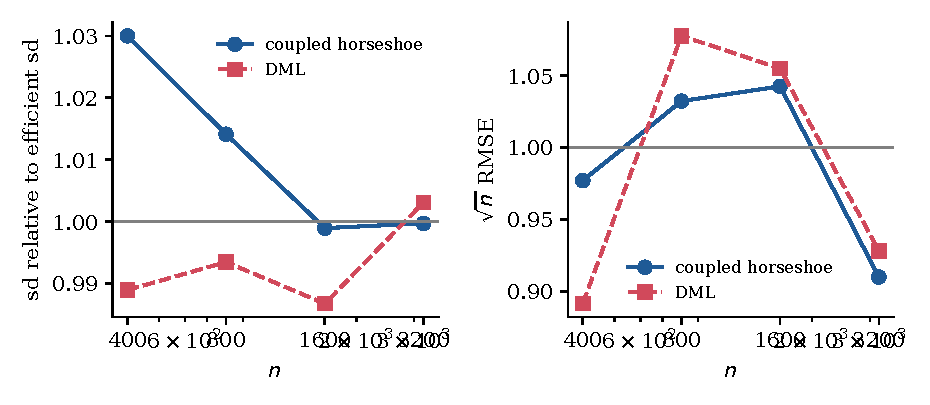
\includegraphics[width=\linewidth]{open_bvm.pdf}
\caption{Problem 1 at larger sample sizes, 40 replications each. Left: posterior standard deviation of the coupled horseshoe, and DML's standard error, relative to the efficient standard deviation. Right: $\sqrt{n}$ times the root mean squared error; the efficient value is one.}
\label{fig:openbvm}
\end{figure}

\paragraph{A sketch.} In the linear Gaussian model with known $\gamma$ and error standard deviation $\sigma$ and the propensity direction unpenalized, let $H$ be the projection onto the intercept and $X\gamma$, and let $r = (I - H)T = (I - H)\nu$. Integrating out the flat priors on the intercept and the coefficient of $X\gamma$ gives
\[
\tau \mid \beta, D \sim N\Big(\frac{r^\top(Y - X\beta)}{r^\top r}, \frac{\sigma^2}{r^\top r}\Big),
\]
whose centre at a draw of $\beta$ differs from its centre at the true $\beta_0$ by $-r^\top X(\beta - \beta_0)/r^\top r$. Since $r^\top r/n \to \mathrm{Var}(\nu)$, the variance is the efficient one, and a Bernstein von Mises theorem follows once the horseshoe posterior puts mass tending to one in probability on $|r^\top X(\beta - \beta_0)| \le \epsilon\sqrt{n}$, for every $\epsilon > 0$. The coupling proposition of Appendix~\ref{app:theory}, an argument to first order, says why this projected error should be small: $I - H$ removes the component of $X(\beta - \beta_0)$ along $X\gamma$, the direction in which shrinkage biases $\tau$. Showing that the horseshoe posterior meets the condition, which means controlling the mixture over its scales, is the open part.

\paragraph{Conjecture.} With $\gamma$ estimated by a horseshoe regression of $T$ on $X$, and sparsities $s_\beta$, $s_\gamma$ satisfying $s_\beta s_\gamma\log^2 p = o(n)$, and conditions on the design and the horseshoe scales that give the corresponding contraction rates, the posterior of $\sqrt{n}(\tau - \hat\tau)$, with $\hat\tau$ an efficient estimator, converges in total variation to the efficient normal law. This is DML's product rate condition, transcribed to sparsity. The simulations above plug in a lasso fit of the propensity instead, so they bear on this conjecture only indirectly.

\section{Problem 2: Coupling for nonlinear nuisances}

\paragraph{Setting.} For nonlinear $g$ and $m$, the coupled prior\index{coupled prior!for nonlinear nuisances|textbf} must protect the directions of function space in which $m$ varies.

\paragraph{Constructions.} There are three candidates. A Gaussian process prior\index{Gaussian process!for nonlinear nuisances|textbf} on $g$ with a kernel $k(x, x') + \lambda\,\hat m(x)\hat m(x')$, whose second term weakens the shrinkage in the estimated propensity direction and removes it as $\lambda \to \infty$, generalizes the propensity covariate. A Dirichlet additive regression tree prior shared between outcome and treatment forests, learning splitting probabilities jointly, generalizes shared local scales. A neural network passing a learned propensity embedding to the baseline but not the effect, as GenTE does, likewise generalizes the propensity covariate.



\begin{proposition}
Let $g \sim \mathrm{GP}(0, k + \lambda\,\hat m\hat m^\top)$ with $\hat m$ a fixed function, $\tau$ with a flat prior, Gaussian errors, and the sample vectors of $T$ and $\hat m(X)$ linearly independent. The posterior of $\tau$ equals the posterior under the prior $g = g_0 + \delta\,\hat m$ with $g_0 \sim \mathrm{GP}(0, k)$ and $\delta \sim N(0, \lambda)$ independent, and as $\lambda \to \infty$ it converges to the posterior under a flat prior on $\delta$, that is, to the model with $\hat m$ as an unpenalized covariate.
\end{proposition}

\begin{proof}
A Gaussian process with kernel $k + \lambda\hat m\hat m^\top$ is the sum of independent processes with kernels $k$ and $\lambda\hat m\hat m^\top$, and the second is $\delta\hat m$ with $\delta \sim N(0, \lambda)$. Integrating $g_0$ out leaves a linear model in $(\tau, \delta)$ with covariance $K + \sigma^2 I$ ($K$ the matrix of $k$ at the sample points, $\sigma^2$ the error variance) and prior $N(0, \lambda)$ on $\delta$; letting $\lambda \to \infty$ gives the flat prior limit, which is generalized least squares of $Y$ on $(T, \hat m)$ with that covariance.
\end{proof}

The first order argument of Appendix~\ref{app:theory}, which treats the propensity as known, suggests that its conclusion still holds when $\hat m$ is only consistent.

\paragraph{Evidence.} We simulated a partially linear model with $n = 300$ and five independent standard normal covariates,
\[
T = m(X) + \nu, \qquad Y = T + g(X) + \varepsilon,
\]
with standard normal $\nu$ and $\varepsilon$, a nonlinear treatment surface $m(x) = \sin(1.5x_1) + 0.5x_2^2 - 0.5 + 0.8x_3$ and an outcome surface $g = 2m + 0.5\cos x_4$, so that $\tau = 1$ and confounding runs through the whole shape of $m$. The propensity surface was estimated by a Gaussian process regression of $T$ on $X$ with a kernel tuned on the whole sample and predictions cross fitted in two folds so that they do not absorb the treatment noise; their correlation with the truth averaged 0.96.

Table~\ref{tab:opengp} and Figure~\ref{fig:opengpcouple} compare a plain Gaussian process prior on $g$ with kernel
\[
k(x, x') = a\exp\Big\{-\frac{1}{2}\sum_{j=1}^{5}\frac{(x_j - x'_j)^2}{\ell_j^2}\Big\},
\]
the coupled kernel at $\lambda = 10$ and $10^3$, and the covariate construction, under three choices of the amplitude $a$, the length scales $\ell_j$ and the noise variance. Strong fixes $a = 1$, every $\ell_j = 1.5$ and the noise variance at its true value 1. Tuned estimates all of them by marginal likelihood in a regression of $Y$ on $X$ alone, whose residual $\nu + \varepsilon$ has variance 2, so the tuned noise variance also absorbs the treatment noise and the tuned prior differs from the strong one in its likelihood as well as in its kernel. True noise keeps the tuned amplitude and length scales and fixes the noise variance at 1, which separates the two.

\begin{table}[ht]
\centering
\caption{Coupling a Gaussian process prior through the propensity direction, 40 replications. The truth is $\tau = 1$. Strong is the prior with fixed hyperparameters, Tuned the prior tuned by marginal likelihood, and True noise the tuned prior with the noise variance set to its true value. Monte Carlo standard errors are 0.011 to 0.013 for the biases and 0.007 to 0.012 for the root mean squared errors.}
\label{tab:opengp}
\small
\begin{tabular}{lcccccc}
\toprule
& \multicolumn{2}{c}{Strong} & \multicolumn{2}{c}{Tuned} & \multicolumn{2}{c}{True noise} \\
Construction & Bias & RMSE & Bias & RMSE & Bias & RMSE \\
\midrule
Plain Gaussian process & 0.528 & 0.534 & 0.029 & 0.077 & 0.016 & 0.072 \\
Kernel $k + 10\,\hat m\hat m^\top$ & 0.186 & 0.203 & 0.037 & 0.080 & 0.021 & 0.071 \\
Kernel $k + 10^3\,\hat m\hat m^\top$ & 0.185 & 0.203 & 0.038 & 0.080 & 0.021 & 0.071 \\
Propensity covariate & 0.185 & 0.203 & 0.038 & 0.080 & 0.021 & 0.071 \\
\bottomrule
\end{tabular}
\end{table}

\begin{figure}[ht]
\centering
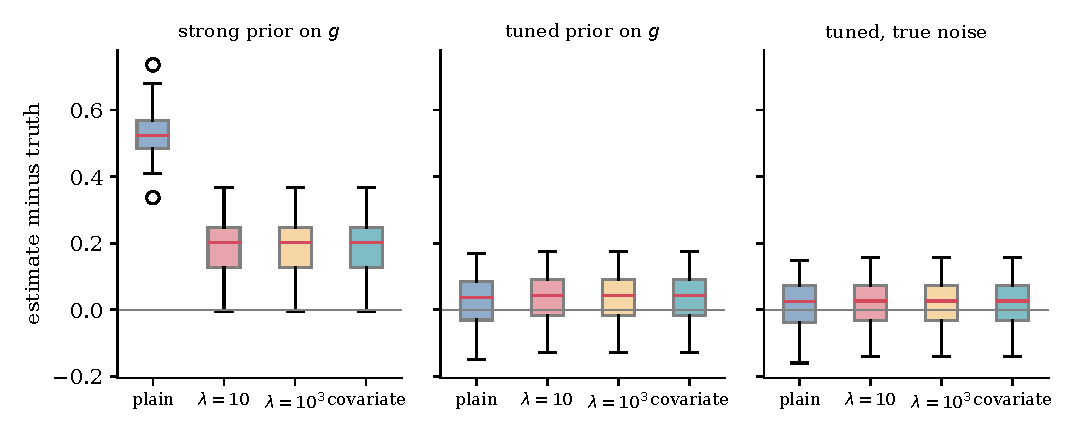
\includegraphics[width=\linewidth]{open_gpcouple.pdf}
\caption{Error of four Gaussian process constructions of the partially linear model under a strong prior, a tuned prior and a tuned prior with the true noise variance on the outcome surface, 40 replications.}
\label{fig:opengpcouple}
\end{figure}

Under the strong prior, regularization induced confounding\index{regularization induced confounding} is severe for the plain process, a bias of half the effect with no coverage. Coupling removes two thirds of it, although its intervals still cover in only 10 of 40 replications. The remainder comes from what the coupling leaves unprotected, which this simulation does not separate, most plausibly the error in $\hat m$, which leaves part of $2m$ outside the span of $\hat m$; the term $0.5\cos x_4$ does not involve the treatment surface. The kernel at $\lambda = 10^3$ and the covariate agree to three decimals, as the proposition says, and $\lambda = 10$ is already close.

Under the tuned prior the plain process has almost no bias and coupling changes nothing, because a prior whose amplitude matches the signal barely shrinks, and regularization induced confounding is a consequence of shrinkage. Every tuned construction covers in 40 of 40 replications, but that is the work of the tuned noise variance, which absorbs the treatment noise and widens the intervals. With the true noise variance the bias stays small (0.016 for the plain process and 0.021 for the coupled constructions, each with Monte Carlo standard error 0.011), the intervals are about 30 percent narrower, and they cover in 37 and 36 of 40 replications, within sampling error of 95 percent. For Gaussian processes the problem therefore seems to live in the hyperparameters: a process tuned to the outcome did well at this dimension and sample size, and the coupling is insurance for the cases, high dimension or small samples, where the prior must shrink. Which cases those are is the open part.

\paragraph{Conjecture.} The shared Dirichlet tree prior makes regularization induced confounding negligible at the root $n$ scale for tree ensembles under the sparsity conditions of Problem 1, with $s_\beta$ and $s_\gamma$ replaced by the numbers of relevant splitting variables, but, like shared horseshoe scales, also protects instruments (Problem 9).

\section{Problem 3: Robins and Ritov with an unknown propensity}

\paragraph{Setting.} In the cell model of Section~\ref{sec:rrw}, the selection probability $e$ is unknown and must be learned from $R$\index{Robins and Ritov example!with an unknown propensity|textbf}.

\paragraph{What we expect.} Every unit informs $e$ through $R$, while only selected units inform $\vartheta$. Under a prior on $e$ smooth in a known feature of the cells, its posterior contracts at that model's rate, and the coupled prior of \eqref{eq:coupled} with $e$ replaced by its posterior draw should inherit root $n$ consistency when $e$ is estimated fast enough and the regression of $\logit\vartheta$ on $\logit e$ is correctly specified. How fast is part of the problem. An error in $e$ enters the fitted curve $q_\xi\{e(x)\}$ of Section~\ref{sec:rrw} at first order, so the $n^{-1/4}$ rate of the doubly robust product would be enough only if the coupled posterior cancels that first order term, as a doubly robust estimator does, and we have no proof that it does.

\paragraph{Evidence.} We repeated the simulation of Section~\ref{sec:rrw}, $K = 20{,}000$ cells and $n = 2{,}000$ units, with a cell feature $z$ and the selection probability learned from $(z, R)$ on every unit by a logistic regression in $z$, fitted by maximum likelihood and plugged in as the simplest stand in for a smooth prior. The coupled estimate is the empirical Bayes version of Section~\ref{sec:rrw}, with the uncertainty in both fitted regressions ignored. The feature $z$ is uniform on $[-1, 1]$. In the first design $e = 0.05 + 0.9\expit(2.5z)$; in the second $e$ is uniform on $[0.05, 0.95]$ independently of $z$, as in Section~\ref{sec:rrw}, so $z$ says nothing about $e$, and with ten times as many cells as units most cells are never visited; in the regime $K/n \to \infty$ of that section no estimator of $e$ is consistent.

Figure~\ref{fig:openrrwunknown} shows 100 replications of four estimators: Horvitz Thompson and the coupled prior, each with $e$ known and with $e$ estimated. When $e$ is smooth, the coupled prior with estimated $e$ has root mean squared error 0.0125, the same as with $e$ known and slightly better than Horvitz Thompson with known $e$ at 0.014. When $e$ is rough, the coupled prior and Horvitz Thompson with the same estimated $e$ are both biased by 0.134: they fail together, for the same reason.

\begin{figure}[ht]
\centering
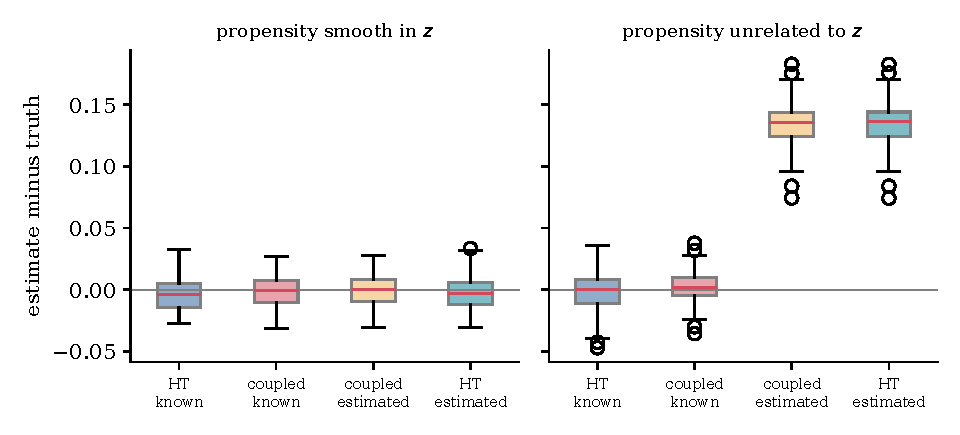
\includegraphics[width=\linewidth]{open_rrw_unknown.pdf}
\caption{The Robins and Ritov example with the selection probability estimated from a cell feature, 100 replications. Left: the selection probability is smooth in the feature. Right: it is unrelated to the feature.}
\label{fig:openrrwunknown}
\end{figure}

\paragraph{Conjecture.} No prior on $(e, \vartheta)$ that is a product of priors on $e$ and on $\vartheta$ given $e$ through a fixed link is uniformly root $n$ consistent over Robins and Ritov's class when $e$ is unrestricted. The simulation is what the conjecture predicts. In this design the boundary is the estimability of the propensity, and the simulation shows no boundary peculiar to Bayesian inference.

\section{Problem 4: Default priors for couplings}

\paragraph{Setting.} The copula of $(Y(0), Y(1))$ is unidentified; Section~\ref{sec:ot} used a Gaussian copula with a prior on $\rho$, and Chapter~\ref{ch:tianpearl} a $\mathrm{Beta}(1/2, 1/2)$ prior on the position within the bounds.

\paragraph{A partial result.} Since the coupling question\index{coupling!default priors for|textbf} does not depend on the scale of measurement, a default prior\index{default prior|textbf} should be invariant under strictly increasing transformations of either outcome. Kendall's $\tau_K$\index{Kendall tau@Kendall's tau|textbf} and Spearman's $\rho_S$ are invariant, and within the Gaussian family $\tau_K = (2/\pi)\arcsin\rho$. A uniform prior on $\tau_K \in [-1, 1]$ is therefore invariant and induces the prior
\[
p(\rho) = \frac{1}{\pi\sqrt{1 - \rho^2}}, \qquad -1 < \rho < 1,
\]
the arcsine law\index{arcsine prior|textbf}. It puts more mass near the comonotone and countermonotone extremes than a uniform prior on $\rho$: the horseshoe shape that appeared for the position within the Tian and Pearl bounds.

\paragraph{Why the reference prior criterion does not decide.} It is tempting to ask for a reference prior\index{reference prior|textbf} in Bernardo's sense, the prior that maximizes the expected Kullback and Leibler divergence between prior and posterior for the fraction helped. But with the marginals known the data carry no information about $\rho$, so the posterior for $\rho$ equals its prior, the divergence is zero for every prior, and the criterion is empty, as it is for any functional of an unidentified parameter. Invariance alone does not fix the prior either, since every prior on $\tau_K$ is invariant to monotone transformations. The case for the arcsine law is that it is uniform on the concordance probability, which is what Kendall's $\tau_K$ measures: a flat prior on the probability that two random individuals are ordered the same way under both treatments.

\paragraph{What the choice costs.} Figure~\ref{fig:openarcsine} shows the prior it induces on the fraction helped for a mean shift of half a standard deviation, against the uniform prior on $\rho$. The arcsine prior gives mean 0.70 against 0.67 and puts 12\% of its mass above 0.9 against 4\%, because it allows near comonotone couplings. The two priors agree on the lower part of the range, where the data from a twin or crossover design can bite (Problem 7), and differ in a region that only an assumption can rule in or out. We recommend reporting the fraction helped under both, as a sensitivity analysis in the sense of Section~\ref{sec:sensitivity}.

\begin{figure}[ht]
\centering
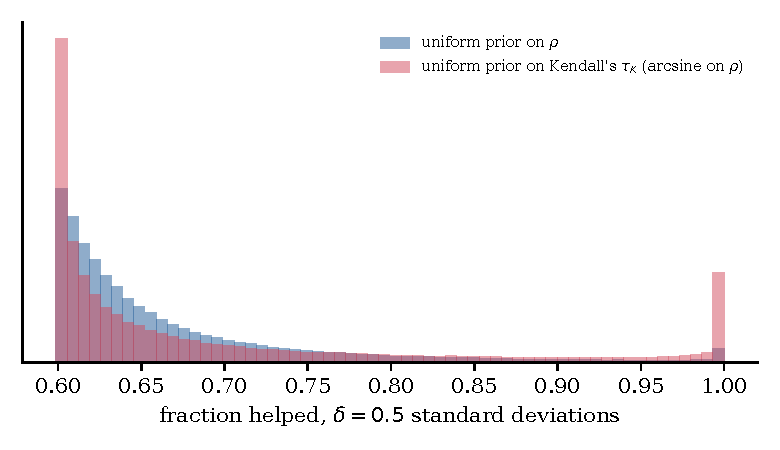
\includegraphics[width=0.9\linewidth]{open_arcsine.pdf}
\caption{Priors induced on the fraction helped, $P\{Y(1) > Y(0)\}$, by a uniform prior on the Gaussian copula correlation and by the arcsine prior that is uniform on Kendall's $\tau_K$, for a mean shift of half a standard deviation.}
\label{fig:openarcsine}
\end{figure}

\paragraph{Open question.} Find a design, short of observing both potential outcomes, whose likelihood depends on $\tau_K$ so that the reference criterion becomes nonvacuous; crossover trials with carryover are the natural candidate.

\section{Problem 5: Combining experiments and observations across populations}

\paragraph{Setting.} An experiment on population $A$ gives $\Prob_A(y_x)$ and $\Prob_A(y_{x'})$; an observational study on population $B$ gives the joint law of $(X, Y)$ there\index{open problems!combining experiments and observations|textbf}. The target is $\PN$ in $B$\index{probability of necessity}.

\paragraph{A model.} Let conditional effects given covariates $W$ transport\index{transportability} up to a discrepancy: $\logit\Prob_B(y_x \mid w) = \logit\Prob_A(y_x \mid w) + \delta_x$ with $\delta_x \sim N(0, s^2)$, and similarly for $x'$. With $W$ measured in both populations, averaging over $B$'s covariate law gives the experimental arm probabilities in $B$, and substitution gives its Tian and Pearl bounds.

\paragraph{What we expect.} As $s \to 0$ the posterior of the bounds on $\PN_B$ concentrates on the Tian and Pearl bounds evaluated at the transported margins; a posterior for $\PN_B$ itself also needs a prior on its position within the bounds, as in Chapter~\ref{ch:tianpearl}. As $s$ grows the posterior of the bounds spreads continuously toward the observational bounds, provided the transported arm probabilities stay compatible with $B$'s observational law, which puts $\Prob_B(y_{x'})$ between $\Prob_B(x', y)$ and $\Prob_B(x', y) + \Prob_B(x)$; the model above does not impose this, and the simulation below does, by restricting the prior on $\Prob_B(y_{x'})$ to that range. Every $s > 0$ then gives the whole range positive probability, and as $s \to \infty$ the prior tends to one uniform on the logit scale over the range, so even an infinite $s$ leaves a prior inside the observational bounds, not the bounds alone. The posterior interpolates between full transport and none, and the prior on $s$ states how far the experiment is believed to travel.

\paragraph{Negative controls inform the transport scale.} A negative control outcome\index{negative control|textbf} is unaffected by treatment but differs between populations for the same reasons as the outcome of interest. With logit discrepancies also drawn from $N(0, s^2)$, each control observed in both populations supplies one observation on $s$; several give a posterior.

With no covariates $W$, we simulated population $B$ from a structural model with a binary confounder $U$, with $\Prob(U = 1) = 0.5$, $\Prob(X = 1 \mid U = 1) = 0.6$, $\Prob(X = 1 \mid U = 0) = 0.2$ and $\Prob(Y = 1 \mid X, U) = 0.7$, $0.4$, $0.3$ and $0.1$ for $(X, U) = (1, 1)$, $(1, 0)$, $(0, 1)$ and $(0, 0)$, so that $\PN_B$ has true bounds $[0.60, 1]$, placed the experiment in a population $A$ whose arm probabilities differ by discrepancies with $s = 0.5$, and observed six negative controls, with standard normal baseline logits in $A$, in both populations with 2{,}000 units each. The arm probabilities of $A$ and the observational law of $B$ were treated as known, each negative control's probability in $A$ was fixed at its observed proportion (which leaves its sampling error out of the posterior for $s$), and the prior on $s$ was uniform on $(0, 2]$.

Only $B$'s untreated arm probability enters the bounds, and $B$'s observational law confines it to $[\Prob_B(x', y), \Prob_B(x', y) + \Prob_B(x)] = [0.10, 0.50]$, so the prior on it is restricted to that interval, which removes almost nothing at $s \le 0.25$ and 3, 28 and 58 percent of the prior mass at $s = 0.5$, 1 and 2. The bounds are monotone in this one probability, so the quantiles below are exact.

Figure~\ref{fig:opentransport} shows the result. Transporting $A$'s arm probabilities as if $s = 0$ gives a lower bound of 0.49, below the truth, with no uncertainty. The posterior for $s$ from the six controls has mean 0.37 and 95\% interval $[0.18, 0.76]$ around the true 0.5. At $s = 0.25$ the posterior 5\% quantile of the lower bound is 0.16; from $s = 0.5$ on it is zero, which is the observational bound. Integrating over the posterior for $s$ gives a lower bound whose median is 0.48 and whose 5\% quantile is zero: six negative controls say the experiment travels, but not well enough to rule out the observational bound.

\begin{figure}[ht]
\centering
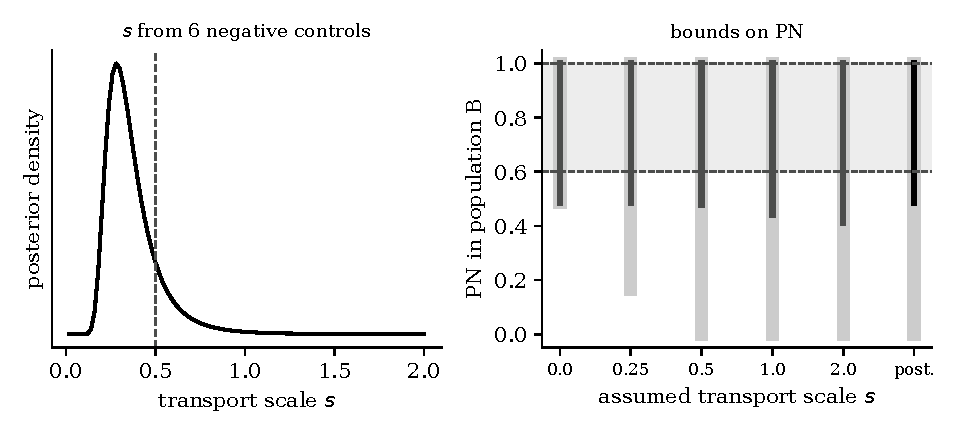
\includegraphics[width=\linewidth]{open_transport.pdf}
\caption{Transporting an experiment. Left: posterior for the transport scale $s$ from six negative control outcomes, true value dashed. Right: bounds on the probability of necessity in population $B$ at fixed values of $s$ and integrated over its posterior (thick lines are posterior medians of the two bounds, light bars the 5\% and 95\% quantiles); the band between the dashed lines is the true bounds.}
\label{fig:opentransport}
\end{figure}

\paragraph{Open question.} How many negative controls, with what prevalence, are needed for the posterior of $s$ to be useful, and when does the assumption that they share the outcome's transport scale fail in a detectable way?

\section{Problem 6: Calibration of amortized posteriors}

\paragraph{Setting.} An amortized posterior\index{amortized posterior|textbf} $G(s(D), U)$ can pass a calibration check that averages over the prior predictive and still be wrong at a particular data set. Section~\ref{comp:sec:checks} gives a local diagnostic, simulation based calibration\index{simulation based calibration!local|textbf} run near the observed data set, and a correction by importance reweighting that we expect to work and have not run.

\paragraph{What is known.} On a network retrained with the design of the two arm trial of that chapter the diagnostic, with 400 local simulations and 19 draws each, finds a flat rank histogram at the observed trial, 18 of 50 and 27 of 50 successes (chi squared 24.0 on 19 degrees of freedom, $p = 0.20$), where the amortized posterior is within 0.003 of the exact one in Wasserstein distance. At an extreme trial, 1 of 50 and 49 of 50, the histogram piles up at the top ranks (chi squared 222, $p < 10^{-35}$, in the same run). At so extreme a summary the exact posterior's own local ranks tilt the same way, with a median chi squared of 244 over 200 repeats, and the network's counts agree with the exact posterior's (chi squared 28.4, $p = 0.08$), so the tilt is not by itself evidence against the network. The direct evidence is the comparison with the exact posterior: the network's posterior is shifted down and too wide, its 5\% and 95\% quantiles 0.834 and 0.984 against the exact 0.853 and 0.973, because few training simulations land near a risk difference of 0.9 (Figure~\ref{fig:openlocalsbc}). The diagnostic costs 400 forward passes and 400 simulated trials for each data set. A global calibration check passes; the local diagnostic flags the extreme trial but needs the exact reference to separate network error from the rank tilt caused by conditioning.

\paragraph{Open question.} Bound local calibration error at $s(D)$ by a quantity computable from the training set, to replace the diagnostic with a certificate. Training density alone is insufficient: the extreme trial of Figure~\ref{fig:openlocalsbc} has about three times the error (Wasserstein distance 0.0088 against 0.0032), yet under uniform priors on the arm probabilities every pair of success counts has prior predictive probability $1/51^2$, giving both trials about 23 exact matches among 60{,}000 training simulations. The extreme summary lies at a corner, where the posterior sits near the boundary $\tau \le 1$ and few training effects are as large. Find what a certificate needs beyond training density.

\paragraph{Evidence on mass and position.} To separate the two, we retrained the network of the two arm trial ten times, with different seeds, at each of 15{,}000, 60{,}000 and 240{,}000 training pairs, on summaries drawn either uniformly from the $51 \times 51$ grid of success counts or from a bell, $q(s) \propto \exp\{-8[(y_0 - 25)^2 + (y_1 - 25)^2]/2500\}$, with scale 12.5 in each count (standard deviation 11.1 on the grid). For each summary $p_0$ and $p_1$ were drawn from their exact beta posteriors and $p_1 - p_0$ was the target, so the posterior to be learned is the same in both designs and only the training mass differs. The error at a summary is the Wasserstein distance between the network's posterior and the exact one, computed as the mean absolute difference between the two quantile functions at 200 evenly spaced levels after sorting the network's curve, divided by the exact posterior standard deviation (Figure~\ref{fig:openlocalsbcdensity}). The network's curve is not monotone by construction, and without the sorting the error is larger, by 9 to 20 percent on average over the grid and by up to 50 percent at some summaries; all numbers below use the sorted curve.

With uniform training, where the extreme trial has as much training mass as the typical one, its error at 60{,}000 pairs is 0.29 (standard error over seeds 0.03) against 0.033, nine times larger, and across the grid the error rises with the distance of the summary from the centre (rank correlation 0.61 to 0.84). Under the bell the extreme trial's expected number of training summaries falls from 23 to 1.7 at 60{,}000 pairs, and its error is 2.7 to 2.9 times the uniform value at every training size (0.81 at 60{,}000), while at the typical trial, which gains mass, the error falls by 10 to 14 percent. Position in the summary space accounts for most of the extreme trial's error and training mass for a further factor of about 2.8, so a certificate has to depend on position as well as on the training density.

\begin{figure}[ht]
\centering
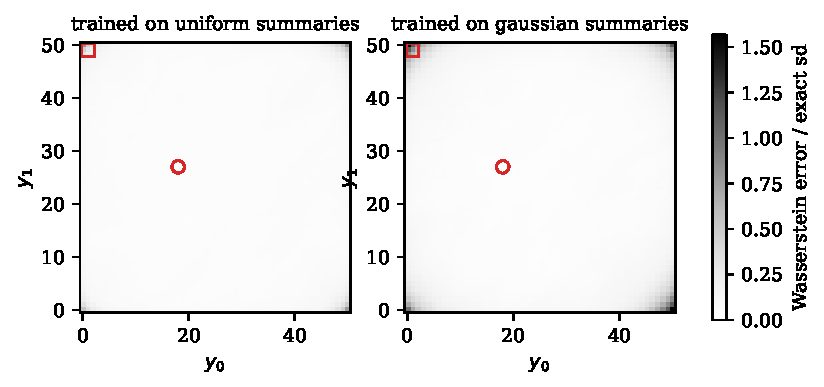
\includegraphics[width=\linewidth]{open_localsbc_density.pdf}
\caption{Wasserstein distance between the network and the exact posterior, divided by the exact posterior standard deviation, at each of the $51 \times 51$ summaries $(y_0, y_1)$, averaged over ten networks trained on 60{,}000 pairs with summaries uniform on the grid (left) or drawn from a bell centred at $(25, 25)$ (right). The circle marks the typical trial and the square the extreme trial of Figure~\ref{fig:openlocalsbc}.}
\label{fig:openlocalsbcdensity}
\end{figure}

\section{Problem 7: Twins and the coupling}

\paragraph{Setting.} In a twin trial\index{twins|textbf} one twin of each pair is treated. Let potential outcomes decompose as $Y(t) = \mu_t + h + e_t$, where $h$ is shared within a pair, has variance $V_h$, and is independent of $(e_0, e_1)$, which are independent across twins with variances $\sigma_t^2 - V_h$.

\begin{proposition}
The covariance between the outcomes of the treated and untreated twins in a pair identifies $V_h$, and the correlation $\rho$ between one person's potential outcomes satisfies
\[
\frac{V_h - s_0s_1}{\sigma_0\sigma_1} \leq \rho \leq \frac{V_h + s_0s_1}{\sigma_0\sigma_1}, \qquad s_t = (\sigma_t^2 - V_h)^{1/2}.
\]
\end{proposition}

\begin{proof}
The twins' outcomes are $\mu_1 + h + e_1$ and $\mu_0 + h + e_0'$ with independent individual terms, so their covariance is $V_h$. For one person, $\mathrm{Cov}(Y(0), Y(1)) = V_h + \mathrm{Cov}(e_0, e_1)$, and the Cauchy and Schwarz inequality bounds the second term by $s_0s_1$ in absolute value.
\end{proof}

With equal unit variances the lower bound is $2V_h - 1$. An unpaired trial allows any $\rho \geq -1$; a twin trial sharing half the variance rules out negative correlation; one sharing 80\% forces $\rho \geq 0.6$. Figure~\ref{fig:opentwins} shows the consequence for the fraction helped\index{fraction helped!twin trials|textbf} when the treated mean is half a standard deviation higher, within the Gaussian copula family: the lower limit rises from 0.60 unpaired to 0.64 when half the variance is shared and 0.71 when 80\% is shared. Student's twins inform not only the average effect but the distribution of individual effects.

\begin{figure}[ht]
\centering
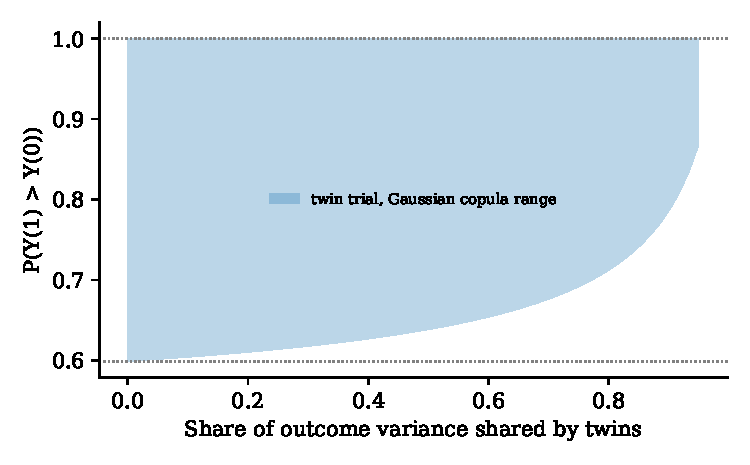
\includegraphics[width=\linewidth]{open_twins.pdf}
\caption{Range of the fraction helped implied by a twin trial, as a function of the share of outcome variance common to twins, for a mean shift of half a standard deviation under a Gaussian copula. Dotted lines mark the range without twins.}
\label{fig:opentwins}
\end{figure}

\paragraph{Beyond the Gaussian copula.} The additive decomposition does more than bound $\rho$. Since $Y(1) - Y(0) = \delta + e_1 - e_0$ with $\delta = \mu_1 - \mu_0$, the shared component cancels from the individual effect, and the fraction helped depends only on the coupling of $(e_0, e_1)$, whose marginals have the identified variances $s_t^2 = \sigma_t^2 - V_h$. The variances do not fix the marginal distributions, but once those are given the Makarov bounds\index{Makarov bounds} of Appendix~\ref{app:theory} apply to them rather than to the full outcomes.

\begin{proposition}
Under the shared component model with Gaussian individual terms of common variance $s^2 = \sigma^2 - V_h$ and $\delta > 0$, for every coupling of $(e_0, e_1)$,
\[
P\{Y(1) > Y(0)\} \geq 2\Phi\Bigl(\frac{\delta}{2s}\Bigr) - 1,
\]
and the bound is sharp. It increases with $V_h$ and tends to one as $V_h \to \sigma^2$.
\end{proposition}

\begin{proof}
The Makarov upper bound on $P(\delta + e_1 - e_0 \leq 0)$, applied to the laws of $\delta + e_1$ and $e_0$, is $1 - \sup_y\{\Phi(y/s) - \Phi((y - \delta)/s)\}$, and the supremum is attained at $y = \delta/2$ with value $2\Phi(\delta/2s) - 1$. Sharpness is Makarov's, and the bound increases with $V_h$ since $s$ decreases.
\end{proof}

With $\sigma = 1$ and $\delta = 0.5$ the Makarov lower bound is 0.20 without twins, 0.28 when half the variance is shared and 0.42 when 80\% is shared; the Gaussian copula range of Figure~\ref{fig:opentwins} sits inside it (Figure~\ref{fig:opentwins2}). The twin design narrows the Makarov range as well as the Gaussian one, by the same mechanism: what the twins share cannot contribute to the spread of individual effects.

\begin{figure}[ht]
\centering
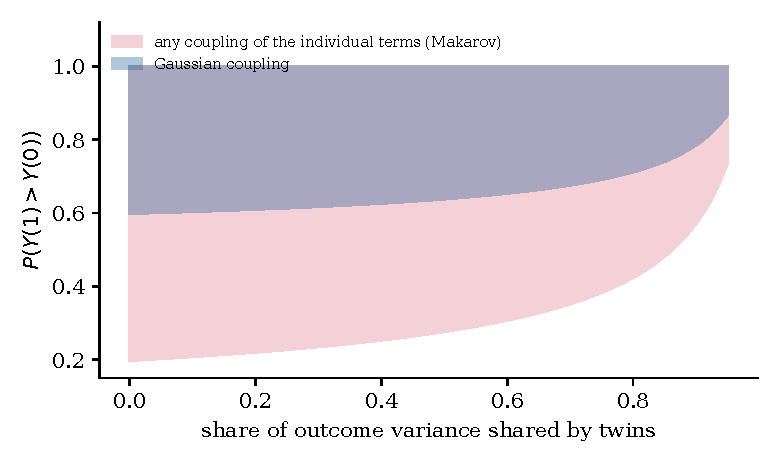
\includegraphics[width=0.9\linewidth]{open_twins2.pdf}
\caption{Range of the fraction helped implied by a twin trial under any coupling of the individual terms, with the Gaussian copula range inside it, for a mean shift of half a standard deviation.}
\label{fig:opentwins2}
\end{figure}

\paragraph{The posterior when the share is estimated.} In a simulated trial of 100 twin pairs, with Gaussian $h$, $e_0$ and $e_1$, $\sigma = 1$, a true shared variance of 0.6 and $\delta = 0.5$, the weighted Bayesian bootstrap\index{Bayesian bootstrap} of the two marginal variances, the within pair covariance and the mean difference gives a posterior for the Makarov lower bound with mean 0.33 and 95\% interval $[0.21, 0.44]$, around a true value of 0.31. 

\paragraph{Open question.} For known non Gaussian individual terms the Makarov theorem of Appendix~\ref{app:theory} already gives the sharp bound, with the supremum no longer at $\delta/2$. The open part is to identify and estimate the distributions of $e_0$ and $e_1$ from the joint law of the twins' outcomes, with honest uncertainty for the resulting bound, and to extend the analysis to covariate dependent shares $V_h(x)$.

\section{Problem 8: Heavy tailed outcomes}

\paragraph{Setting.} The 401(k) outcome\index{401(k) plan!heavy tailed outcome|textbf} has a maximum a thousand times its median, which makes Gaussian posteriors and squared error nuisance learners fragile\index{open problems!heavy tailed outcomes|textbf}.

\paragraph{Evidence.} We simulated the partially linear model of Section~\ref{sec:ricsim} with $n = 300$, 30 standard normal covariates, five confounders with unit coefficients in both equations, standard normal treatment noise, and Student $t$ outcome errors on two degrees of freedom, with infinite variance. Over 30 replications we compared the coupled horseshoe with Gaussian errors, the same prior with Student $t$ errors\index{Student t errors} on three degrees of freedom as a scale mixture of normals, and DML with lasso nuisances.

\begin{table}[ht]
\centering
\caption{Heavy tailed errors, 30 replications.}
\label{tab:openheavy}
\small
\begin{tabular}{lccc}
\toprule
Method & RMSE & Coverage & Width \\
\midrule
Coupled horseshoe, Gaussian errors & 0.174 & 28/30 & 0.65 \\
Coupled horseshoe, Student $t$ errors & 0.086 & 29/30 & 0.32 \\
DML, lasso nuisances & 0.183 & 25/30 & 0.54 \\
\bottomrule
\end{tabular}
\end{table}

\begin{figure}[ht]
\centering
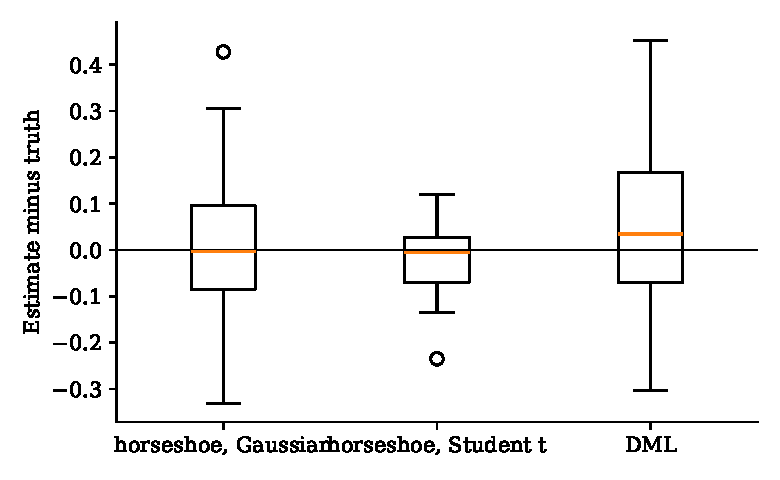
\includegraphics[width=\linewidth]{open_heavy.pdf}
\caption{Error of three estimators of $\tau = 1$ with infinite variance errors, 30 replications.}
\label{fig:openheavy}
\end{figure}

The Student $t$ model halves the error of both alternatives and the interval width of the Gaussian model, with coverage near nominal (Table~\ref{tab:openheavy} and Figure~\ref{fig:openheavy}). DML's intervals covered in only 25 of 30 replications. The larger study below, with errors on 2 degrees of freedom and 200 replications at each $n$, gives DML coverage of 92 percent at $n = 200$ and 95.5 percent at $n = 400$, so the shortfall here is probably in part a low draw from 30 replications.

\paragraph{Rates.} The DML score is a sample average of terms with the same tail index as the errors, so for errors in the domain of attraction of a stable law with index $\alpha \in (1, 2)$ and nuisance errors small enough not to matter, its error is of order $n^{-(1 - 1/\alpha)}$ up to a slowly varying factor, slower than $n^{-1/2}$; the Student $t$ working model\index{Student t errors} gives an M estimator whose influence is bounded in the residual, though not in the covariates, and should keep the root $n$ rate.

We simulated the design above at $n = 100$, 200, 400, 800, 1{,}600, 3{,}200 and 6{,}400 with 200 replications at each $n$, for errors that are $t$ on 1.5 degrees of freedom, where the predicted DML exponent is $-1/3$, $t$ on 2 degrees of freedom, and Gaussian. Besides the Student $t$ posterior mean, the posterior mean under Gaussian errors and DML, we computed an oracle: the DML score with the true nuisances in place of fitted ones, the sum of $\nu\varepsilon$ over the sum of $\nu^2$. Figure~\ref{fig:openrates} plots the median absolute error for errors on 1.5 degrees of freedom, with bootstrap intervals; the slopes below are least squares fits of log median error on log $n$ over $n \ge 400$, with 95\% bootstrap intervals. The Student $t$ posterior mean falls with slope $-0.55$ ($-0.63$ to $-0.49$), consistent with the root $n$ rate, and its intervals cover in 94 to 98 percent of replications at every $n$. DML's median error falls with slope $-0.31$ ($-0.38$ to $-0.23$), close to the predicted $-1/3$, and so do the oracle's ($-0.27$) and the Gaussian posterior mean's ($-0.31$): the slow rate belongs to the squared error score under heavy tails, not to the estimation of the nuisances. At $n = 1{,}600$ the median error of DML is 4.9 times that of the Student $t$ posterior mean, and at $n = 6{,}400$ it is 6.5 times. A few replications with extreme errors dominate the root mean squared error of DML, 2.03 at $n = 200$ and then 0.50, 0.35 and 0.30 at $n = 400$, 800 and 1{,}600, against 0.075, 0.049 and 0.034 for the Student $t$ posterior mean.

With errors on 2 degrees of freedom the gap shrinks to a factor of about two and both slopes are close to $-1/2$ ($-0.50$ for the Student $t$ posterior mean and $-0.52$ for DML). This is the boundary case: the oracle score's error is of order $\sqrt{\log n/n}$, a logarithmic factor that slopes over this range of $n$ cannot detect. With Gaussian errors there is no gap. For errors on 1.5 degrees of freedom DML's Wald intervals covered 89 and 91.5 percent of replications at $n = 100$ and 200 and 95.5 to 97 percent at $n \ge 800$, where the Monte Carlo standard error of each coverage is about 1.5 percentage points.

\begin{figure}[ht]
\centering
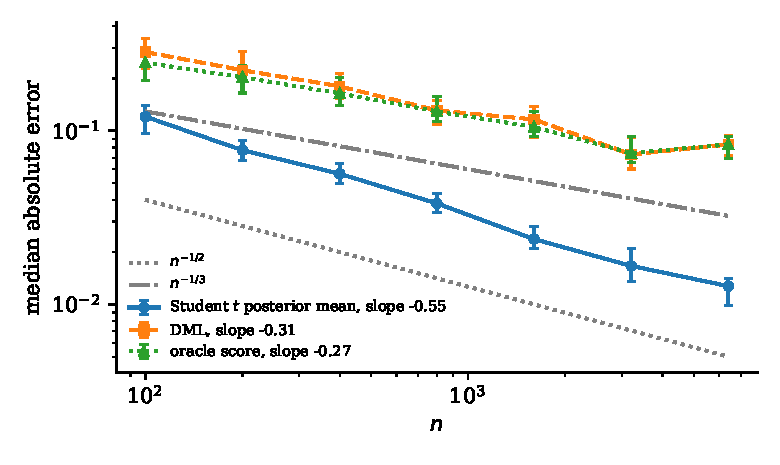
\includegraphics[width=0.9\linewidth]{open_rates.pdf}
\caption{Median absolute error of the Student $t$ posterior mean, DML and the oracle score as $n$ grows, with bootstrap 95\% intervals, for errors on 1.5 degrees of freedom and 200 replications at each $n$; reference lines for the $n^{-1/2}$ and $n^{-1/3}$ rates.}
\label{fig:openrates}
\end{figure}

\paragraph{Conjecture.} For errors in the domain of attraction of a stable law with index $\alpha \in (1, 2)$, the posterior under a Student $t$ working model with fixed degrees of freedom contracts at the root $n$ rate and is asymptotically normal around the corresponding M estimator, with variance the inverse of the expected negative Hessian of the working log likelihood, not the sandwich variance of Section~\ref{sec:bg:large} that governs the sampling error of that estimator (Kleijn and van der Vaart 2012). Its credible intervals then have nominal coverage only if the two variances agree, and otherwise only after a sandwich correction. DML with squared error nuisances has error of order $n^{-(1 - 1/\alpha)}$, up to a slowly varying factor, and Wald intervals whose limiting coverage need not be the nominal one, since a self normalized sum is asymptotically normal only when its terms lie in the domain of attraction of the normal law (Gin\'e, G\"otze and Mason 1997). In the simulation above the departure from nominal coverage was too small to see for $n \ge 800$.

\section{Problem 9: Coupling that protects confounders but not instruments}

\paragraph{Setting.} Chapter~\ref{ch:horseshoe} showed that sharing local scales between outcome and treatment coefficients protects instruments along with confounders\index{coupled prior!protecting confounders but not instruments|textbf}.

\paragraph{A construction.} Give each covariate a shared scale $\lambda_j$ and a private outcome scale $\eta_j$:
\[
\beta_j \sim N(0, \lambda_j^2\eta_j^2\tau_{\mathrm{g},Y}^2\sigma_Y^2), \quad \gamma_j \sim N(0, \lambda_j^2\tau_{\mathrm{g},T}^2\sigma_T^2), \quad \lambda_j, \eta_j \sim C^+(0,1).
\]
A large $\gamma_j$ makes $\lambda_j$ large, and the private scale $\eta_j$ was meant to keep $\beta_j$ shrunk unless the outcome model supplies evidence of its own; below we find that it does so only in part. With the auxiliary variables $\nu_j$ of the mixture of Section~\ref{sec:hsregression}, the full conditionals of the squared scales are inverse gamma; the square $\lambda_j^2$ of the shared scale has shape $3/2$ and rate $1/\nu_j + \beta_j^2/(2\eta_j^2\tau_{\mathrm{g},Y}^2\sigma_Y^2) + \gamma_j^2/(2\tau_{\mathrm{g},T}^2\sigma_T^2)$.

\paragraph{Evidence.} We repeated the instrument design of Section~\ref{sec:sharedsim} with 40 fresh replications, so figures for independent and shared scales differ slightly from that section, and four priors: independent scales, shared scales, the product prior\index{coupled prior!product form}, and independent scales with the estimated propensity as an unpenalized covariate, all fitting treatment and outcome models jointly.

\begin{table}[ht]
\centering
\caption{Four coupling strategies in a design with moderate confounders, instruments and prognostic covariates, 40 replications.}
\label{tab:openprod}
\small
\begin{tabular}{lcccc}
\toprule
Prior & Bias & RMSE & Coverage & Width \\
\midrule
Independent scales & 0.018 & 0.038 & 38/40 & 0.17 \\
Shared scales & 0.035 & 0.083 & 37/40 & 0.29 \\
Product of shared and private & 0.021 & 0.050 & 38/40 & 0.21 \\
Propensity covariate & $-$0.003 & 0.088 & 36/40 & 0.31 \\
\bottomrule
\end{tabular}
\end{table}

\begin{figure}[ht]
\centering
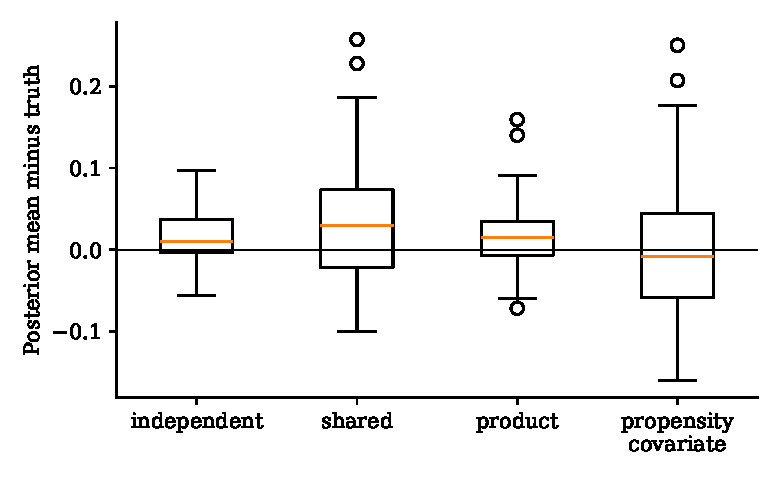
\includegraphics[width=\linewidth]{open_product.pdf}
\caption{Error of four coupling strategies in the instrument design, 40 replications.}
\label{fig:openproduct}
\end{figure}

The product prior recovers most of what shared scales lose, cutting error from 0.083 to 0.050 (Figure~\ref{fig:openproduct}) and interval width from 0.29 to 0.21 (Table~\ref{tab:openprod}). The propensity covariate is nearly unbiased but has the largest error: the five instruments dominate the estimated propensity, and adding it to the outcome model imports their variance. Here independent scales are best, which we attribute mainly to the instruments raising the variance of the treatment and so shrinking the bias of either prior (Exercise~\ref{ex:ch07:7} compares the design without instruments). In the design of Section~\ref{sec:ricsim}, with no instruments and confounders driving both models strongly, coupling to the whole sample propensity covariate cut the independent horseshoe's bias from 0.059 to $-0.023$, although DML had the smaller error. Every coupling device trades bias protection against variance from instruments.

\paragraph{What the product prior does to an instrument.} The product prior does not shrink a pure instrument's outcome coefficient as the independent prior does. Conditional on the shared scale $\lambda_j$, the outcome coefficient $\beta_j$ has a horseshoe prior with global scale $c = \lambda_j\tau_{\mathrm{g},Y}$. For an instrument the treatment model makes $\lambda_j$ large, and a horseshoe with a large global scale shrinks little. Figure~\ref{fig:openproduct2} computes the posterior shrinkage weight $\E(\kappa_j \mid y)$ of a coefficient whose standardized estimate is $y$, as a function of $c$: at $y = 0$, pure noise, the weight is 0.67 at $c = 1$ but 0.33 at $c = 10$ and 0.24 at $c = 30$. The product prior therefore protects an instrument only partially, which is why its error in Table~\ref{tab:openprod} lies between the independent and shared priors.

\begin{figure}[ht]
\centering
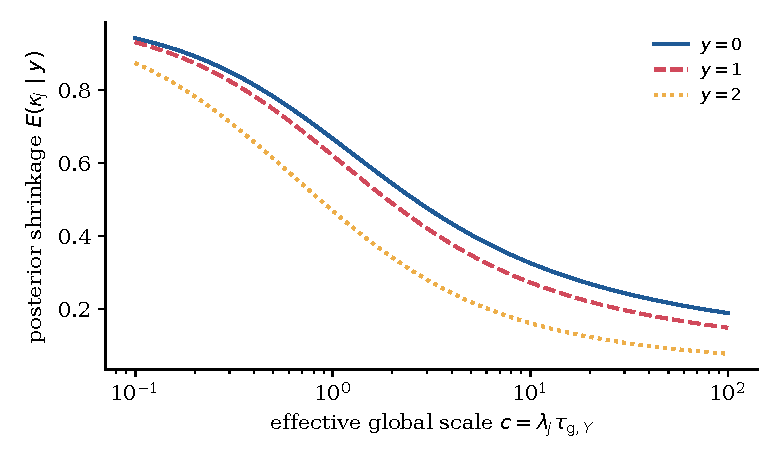
\includegraphics[width=0.85\linewidth]{open_product2.pdf}
\caption{Posterior shrinkage weight of an outcome coefficient under a horseshoe with global scale $c$, for standardized estimates $y = 0$, 1 and 2. Under the product prior an instrument's $c$ is large, so its coefficient is shrunk less.}
\label{fig:openproduct2}
\end{figure}

\paragraph{A limit on coordinatewise coupling.} Any prior whose scale for $\beta_j$ increases with the evidence for $\gamma_j$ protects instruments along with confounders: the treatment model cannot distinguish them. Only the outcome model separates them, and the independent horseshoe already uses that evidence through tail robustness. Coupling that protects confounders without instruments must therefore use the outcome evidence as well, or act on directions rather than coordinates. The propensity covariate protects the single direction $X\gamma$, the confounding direction when the covariates driving treatment also drive the outcome and merely a noisy one when they are instruments, which is why it was unbiased but noisy in the table.

\paragraph{Conjecture.} Among priors that are exchangeable across coordinates and depend on the treatment model only through the posterior of $\gamma$, none achieves both the independent prior's variance on instruments and the shared prior's bias protection on confounders. The propensity covariate attains the bias protection, and the residual variance it imports from instruments is the price of a coordinate free coupling.

\section{Problem 10: Teaching}

This problem is not technical\index{open problems!teaching|textbf}. Many courses in economics and epidemiology now teach causal inference with DML and its relatives at the centre, and the model first view, if at all, as an alternative for specialists.

\paragraph{Open question.} Write the introductory course in which students fit a model, report its posterior and compute every causal summary as accounting, with the average treatment effect introduced as the first such summary rather than the object of inference.

Table~\ref{tab:course} gives a ten week outline, with the data set, the computation and the comparison for each week. Every week fits one model, reads several accountings off it, and asks what DML or its relative would have reported and left out. The scripts in the repository of Appendix~\ref{app:code} carry out each week's analysis.

\begin{table}[ht]
\centering
\small
\caption{A ten week course in model first causal inference.}
\label{tab:course}
\setlength{\tabcolsep}{2pt}
\begin{tabular}{@{}cL{1.15in}L{0.85in}L{1.0in}L{0.85in}@{}}
\toprule
Week & Topic & Data & Computation & Compared with \\
\midrule
1, 2 & Potential outcomes, exchangeability, the average effect as accounting & Thornton & logistic model, Polya Gamma Gibbs & difference in proportions \\
3 & Randomization and its failures & Lanarkshire, twins & paired model, posterior for the bias & Student's critique \\
4 & Shrinkage priors and confounding & 401(k) & coupled horseshoe Gibbs & lasso plug in, DML \\
5 & Trees and surfaces & NHEFS, LaLonde & BART, causal forest & matching, weighting \\
6 & Inverse weighting and its critique & simulated cells & Horvitz Thompson, coupled prior & Robins and Ritov \\
7 & Difference in differences & castle doctrine & horseshoe difference in differences & two way fixed effects \\
8 & Instruments & Card & reduced form posterior & two stage least squares \\
9 & Bounds and sensitivity & smoking & posterior inside the bounds & Cornfield, E value \\
10 & The workflow on a project & the student's & all of the above & the student's choice \\
\bottomrule
\end{tabular}
\end{table}

We hope this book is a step toward that course.

\section{Problem 11: Rates for the triangular network posterior}

\paragraph{Setting.} Chapter~\ref{ch:computation} learns the posterior of a parameter $\theta$ of dimension $d$ as a triangular map\index{triangular map!rates for the network posterior|textbf} from uniform noise, each coordinate through its quantile function given the earlier ones, fitted by minimizing the check loss on simulated pairs $(\theta, D)$. The network sees the data through a summary $S(D)$, and its accuracy at the observed summary $s$ is the Wasserstein distance between its posterior and the posterior given $S = s$.

\paragraph{What is known.} By Proposition~\ref{gbc:prop:pinball} a trained network differs from the summary posterior only through finite training, and for that the theory is thin. Section~\ref{comp:sec:summaries} states what we have: rates at one fixed quantile level from Padilla, Tansey and Chen (2022), no rate for the randomly drawn levels our network trains on, and consistency for fully connected ReLU networks (Theorem A.4 of Polson and Sokolov 2026a), which covers neither the product architecture of Section~\ref{comp:sec:network} nor the optimization error. In one dimension the Wasserstein distance is the mean absolute error between the learned quantile function, sorted where it crosses, and the exact one, which is 0.004 for the two arm trial of Chapter~\ref{ch:computation} at its observed data set. That is a value at a chosen data set, not a rate, and Problem 6 shows why uniformity over the summary matters.

\paragraph{Open question.} Give rates, uniform over the observed summary, for the Wasserstein error of the triangular quantile network posterior in $d$ dimensions, as a function of the number of training simulations, the network class and the smoothness of the posterior quantile functions. The posterior's own spread shrinks like $n^{-1/2}$, and rescaling by $\sqrt{n}$ multiplies a Wasserstein distance by $\sqrt{n}$, so a network error $e$ keeps a Bernstein von Mises limit that the exact summary posterior has in Wasserstein distance when $\sqrt{n}\,e \to 0$. The number of training simulations must grow with $n$ fast enough to give that.

\section{Problem 12: Orthogonal summaries}

\paragraph{Setting.} The network of Chapter~\ref{ch:computation} learns the posterior given a summary $S(D)$, which conditions on less than the data\index{open problems!orthogonal summaries|textbf}. For the average effect in the nonparametric model for the outcome regression and the propensity score, the efficiency of that posterior depends on what the summary contains, and we do not know what it must contain.

\paragraph{What is known.} Proposition~\ref{blp:prop:bvm} of Chapter~\ref{ch:blp}, restated in Section~\ref{comp:sec:summaries}, centres the posterior given an asymptotically normal summary at the efficient minimum distance estimator built from it, and makes that posterior asymptotically at least as concentrated as any asymptotically normal estimator of the target that the summary contains. Both statements concern the exact summary posterior, not a trained network. In a correctly specified regular parametric model, summaries that are sufficient or contain an efficient estimator give a posterior that is efficient for that model (Section~\ref{comp:sec:core}).

The nonparametric model is different. A prior that ignores the propensity score can bias the posterior for the average effect at the $\sqrt{n}$ scale. Ray and van der Vaart (2020) repair this by perturbing the prior in the inverse propensity direction (Problem 1), and a generative posterior inherits whatever its prior does. The fitted propensity in the summary of Chapter~\ref{ch:computation} changes what the posterior conditions on, not the prior: a propensity aware prior has to be built into the simulator, and we have no theorem saying which summaries are then enough.

\paragraph{Open question.} Characterize the summaries $S$ for which the summary posterior of an average effect satisfies a semiparametric Bernstein von Mises theorem in the nonparametric model, extending Ray and van der Vaart (2020) from priors to summaries. We call such summaries orthogonal\index{summary statistics!orthogonal|textbf}, after the Neyman orthogonal score of Chapter~\ref{ch:dml}.

\section{Problem 13: Calibration of distorted values}

\paragraph{Setting.} The decision phase of Chapter~\ref{ch:cdt} turns the learned quantile function of utility into a distorted value\index{calibration!of distorted values|textbf}\index{risk sensitive decisions!calibration of distorted values|textbf} $\Vbeta(a)$ for each action $a$ and returns the action with the largest value. In the illustration of Section~\ref{gbc:sec:risk}, two programmes with means 1.00 and 1.08 have conditional value at risk at level 0.25 of 0.56 and $-0.02$, so the choice turns on the lower tail of utility, which no average effect expresses.

\paragraph{What is known.} The checks of Chapter~\ref{ch:computation} are for a parameter: simulation based calibration near the observed data, with a proposed correction by importance reweighting (Section~\ref{comp:sec:checks}). The coverage studies of Chapter~\ref{ch:blp} concern parameters and means. For the action itself, Proposition~\ref{gbc:prop:regret} bounds the regret of the Bayes policy by twice the Lipschitz constant times the concentration of the posterior, for expected utility and under a Lipschitz condition, which holds for an infinite dimensional effect surface in the $L^1$ norm but then needs the posterior mean of that distance to shrink. A finite check in one conjugate design, the conditional value at risk of the risk difference in a two arm trial (Section~\ref{gbc:sec:normal}), finds the network's action different from the exact Bayes action in under 2.3 percent of trials but in 5 to 58 percent of close calls, at small cost.

\paragraph{Open question.} Develop checks corresponding to these for $\Vbeta(a)$ and for the Bayes action itself. Part of the question is what there is to cover, since $\Vbeta(a)$ is a functional of the posterior predictive law of utility, random through $\theta$ as well as $Y(a)$, and not a function of $\theta$ alone.

\section{Problem 14: Time consistency of distortions}

\paragraph{Setting.} In the dynamic treatment regimes of Section~\ref{gbc:sec:dynamic} of Chapter~\ref{ch:cdt}, a policy that learns from the outcomes it generates solves a Bayes adaptive decision process: the value of an action in the first period averages the best second period value, computed from the posterior updated on the first period's outcome. Replacing the expectations in that recursion by distorted values at each stage gives a risk sensitive policy, the stagewise version; distorting the utility of the whole horizon at once gives the whole horizon version.

\paragraph{What is known.}  For distorted values Section~\ref{gbc:sec:dynamic} observes that distorted criteria are not in general time consistent\index{risk sensitive decisions!time consistency|textbf}, so that the stagewise and whole horizon versions can differ. For CVaR at level one half the two versions can choose different first period actions (Exercise~\ref{ex:chgbc:5}), and no other row of Table~\ref{gbc:tab:distortions} is time consistent either, except the risk neutral one (CVaR at $\eta = 1$, Wang at $\eta = 0$ and CPW at $\eta = 1$ are that row). Kupper and Schachermayer (2009) show that a normalized, law invariant criterion that is time consistent, strictly monotone, continuous and has the Fatou property is the certainty equivalent of an expected utility, and that the only law invariant, time consistent and relevant dynamic risk measure is the entropic one. A distortion criterion shifts by $c$ when $c$ is added to the utility and scales by $k > 0$ when the utility is multiplied by $k$, and the only certainty equivalent that does both is the mean, which rules out the Wang, power and CPW rows. CVaR with $\eta < 1$ is not strictly monotone, but it is a relevant coherent risk measure and not the entropic one, so the second result rules it out. For every row except risk neutral, some two period problem therefore gives different stagewise and whole horizon values.

\paragraph{Open question.} For each distortion of Table~\ref{gbc:tab:distortions} (the Wang distortion, the two power distortions, CPW and CVaR across its levels), find the problems of the dynamic setting of Section~\ref{gbc:sec:dynamic} in which the stagewise and whole horizon risk sensitive Bayes policies still choose the same actions, bound the whole horizon value the stagewise policy gives up when they do not, and find whether that loss shrinks as the posterior concentrates.

\section{Problem 15: Which flow an invariant transport selects}

\paragraph{Setting.} Proposition~\ref{gr:prop:transport} turns an invariant transport into a group\index{open problems!flow of an invariant transport|textbf}. When the treatment does the same thing in every covariate cell, the treated law of each cell is the control law pushed through one increasing map $M$ of the line, and the smallest group that contains $M$ is the cyclic group it generates. A dose interpretation of the effect, in which a fraction $s$ of the treatment acts as a group element $g^{s}$ with $g^{1}=M$, needs $M$ to sit inside a one parameter flow.

\paragraph{What is known.} Fort (1955) proved that every increasing homeomorphism of the line embeds in a continuous flow of increasing homeomorphisms, so a flow through $M$ always exists. When $M$ is not the identity the flow is not unique: on each stretch of the line free of fixed points of $M$ it is built from a chart chosen freely on one fundamental domain, and any other choice gives another flow with the same $g^{1}$. The map $M$ therefore fixes the effect of one full dose and no other dose. A smooth flow is singled out under conditions on $M$ at its fixed points (Szekeres 1958; Kopell 1970).

\paragraph{Open question.} For a translation $M$ in the logit chart on $(0,1)$, multiplying the shift by $s$ gives the unique flow smooth up to the fixed endpoints (Szekeres 1958; Kopell 1970), while many flows are smooth on the open interval. Give conditions under which the model or estimated cell laws select one flow through $M$, determining the dose interpretation $g^s$, and say when the choice can only be a convention.

\section{Problem 16: Choosing the scale and testing stability on one data set}

\paragraph{Setting.} Section~\ref{gr:sec:kidney} proposes a prior on the Aranda Ordaz index $\lambda$ for choosing the scale; Proposition~\ref{gr:prop:hstest} tests stability on a given scale with a horseshoe on stratum departures $\eta_j$ from a common effect\index{open problems!choosing the scale and testing stability|textbf}. Applied in sequence, they use the same data to choose the scale and test stability on it.

\paragraph{What is known.} Theorem~\ref{gr:thm:select} gives the rate at which the posterior selects among a finite set of scales under smooth positive priors, with the information gap as the exponent. Proposition~\ref{gr:prop:hstest} gives the Bayes factor of stability on one scale, with different rates under two priors for the global scale $\gscale$. Neither covers a prior on $\lambda$ together with a horseshoe on the scale it selects, and we know of no result on what the test is worth when the scale was chosen from the same data.

\paragraph{Open question.} Give a coherent joint prior on $(\lambda,\psi,\gscale)$ under which the choice of scale and the test of stability on the chosen scale are one posterior, and find its frequency properties: the size of the test of stability when the scale was chosen from the same data, and the rate at which the posterior over $\lambda$ moves towards the boundary of the family as $n$ grows.

\section{Problem 17: A group effect with a nonparametric baseline}

\paragraph{Setting.} Part (b) of Theorem~\ref{gr:thm:recon} gives credible sets for the group effect $g$ with exact coverage under the right Haar prior when the baselines are known\index{open problems!group effect with a nonparametric baseline|textbf}. With an unknown baseline map $\gamma(\cdot)$ under a BART or horseshoe prior the guarantee of exactness is lost (Remark~\ref{gr:rem:nuisance}).

\paragraph{What is known.} A semiparametric Bernstein von Mises theorem for the marginal posterior of $g$ needs conditions on the prior for $\gamma$ that remove the bias from shrinkage of the baseline, the regularization induced confounding\index{regularization induced confounding} of Hahn, Carvalho, Puelz and He (2018) (Chapter~\ref{ch:ipw}). Ray and van der Vaart (2020) remove it for the mean of a binary outcome missing at random by perturbing the prior in the inverse propensity direction. We know of no first order result for the effect of a group action, with right Haar on $g$ and BART on $\gamma$.

\paragraph{Open question.} First, find a prior for $\gamma(\cdot)$, perhaps a coupled prior in the sense of Problem 2, for which the marginal posterior of $g$ has first order correct frequentist coverage. Then ask for a semiparametric version, with right Haar on $g$ and that prior on $\gamma$, whose coverage is exact to second order.

\section{Problem 18: Stability on the affine group}

\paragraph{Setting.} Proposition~\ref{gr:prop:hstest} tests whether an effect is the same in every stratum when the effect is one number, an element of the additive group, with a horseshoe on the departures of the stratum effects from a common one\index{open problems!stability on the affine group|textbf}. On the affine group of Proposition~\ref{gr:prop:affine} the effect has two components, a scale $\sigma$ and a location $\mu$.

\paragraph{What is known.} For one component and at least three strata, under a half Cauchy prior on the global scale in the units of the data, the Bayes factor for stability grows only like $\sqrt n$ when the effect is stable, and the Bayes factor against it grows exponentially in $n$ under a fixed departure (Proposition~\ref{gr:prop:hstest}). On the affine group the scale part of a composite of treatments is order free and the location part is not (Proposition~\ref{gr:prop:affine}), so the two components are stable in different senses, and a test of one departure does not cover both.

\paragraph{Open question.} Extend Proposition~\ref{gr:prop:hstest} to the affine group, testing stability separately for the order free scale component and the order dependent location component, and find the rate of the Bayes factor for each, alone and together, under a horseshoe on the departures of each component.

\section{Problem 19: An equivariant generator for a group effect}

\paragraph{Setting.} For an element $h$ of a group $H$ acting on a response of any dimension, write $P_{x,t}$ for the law of $Y(t)$ given $X=x$ and $h_\#P$ for the law of $hY$ when $Y\sim P$. The structure of Proposition~\ref{gr:prop:transport}, stated there for a real outcome, is then $P_{x,1}=h_\#P_{x,0}$ for every $x$\index{open problems!equivariant generator|textbf}. The GenTE learner of Chapter~\ref{ch:gente} simulates the outcome from uniform noise $u$ through conditional quantile functions $q_t(u\mid x)$ fitted on data from both arms.

\paragraph{What is known.} For a real outcome and increasing $h$ the quantile function of $hY(0)$ given $X=x$ is $h\{F^{-1}_{x,0}(u)\}$, so a generator with $G(u,x,1)=h\{G(u,x,0)\}$, which we call equivariant, needs one baseline generator and one group element in place of two separate generators. In higher dimensions too, if $B(U,x)$ has law $P_{x,0}$, then $hB(U,x)$ has law $h_\#P_{x,0}=P_{x,1}$, for any measurable action. Sharing the noise $u$ between the arms fixes a coupling of $Y(0)$ and $Y(1)$, the comonotone one for a real outcome, which the arm laws do not identify (Section~\ref{sec:ot}); it is a device for simulating the two arms and says nothing about individual effects. What the constraint saves in training cost, and what it does to the approximation error of the network, are open.

\paragraph{Open question.} For a group $H$ indexed by a finite dimensional parameter, with $h$ estimated from the data, find when one baseline network and an estimated $h$ reach a given Wasserstein error in the arm laws with fewer training draws or network parameters than two unrestricted arm generators. Then bound the error the constraint adds when the group structure holds only approximately, with $P_{x,1}$ within $\delta$ of $h_\#P_{x,0}$ in Wasserstein distance uniformly in $x$.

\section{Problem 20: Selection with weak instruments in the reparameterized model}

\paragraph{Setting.} The bivariate normal selection model of Chapter~\ref{ch:frameworks}, the one behind \eqref{ss:eq:mills}, has a latent propensity $T^\ast=X^\top\kappa+Z^\top\eta+V$, a treatment $T=\one\{T^\ast>0\}$ and an outcome $Y=X^\top\beta+\tau T+U$ observed for every unit, with correlation $\rho$ between $U$ and $V$; the instruments in $Z$ enter the selection equation and not the outcome, and the target is $\tau$\index{open problems!selection model with weak instruments|textbf}. Chapter~\ref{ch:iv} sketches its Bayesian treatment by data augmentation and shows what weak instruments do to a posterior. The reparameterization of Chapter~\ref{ch:horseshoe} puts the shrinkage on coordinates in which the nuisance priors do not leak into the effect, for a treatment that is exogenous given $X$.

\paragraph{What is known.} Neither result covers the selection model. With a horseshoe prior on the coefficients of the instruments in the selection equation, weak instruments are shrunk towards zero, and an instrument that is shrunk away leaves the effect identified only through the functional form and through the prior on $\rho$.

\paragraph{Open question.} Extend the reparameterization to the selection model, with a horseshoe on the instrument coefficients and a prior on $\rho$, and determine when weak instruments make the posterior of the effect dominated by the prior. A first step is a simulation with a known $\rho$ and instruments of increasing strength, followed by a theorem on the rate at which the posterior moves from the prior to the data as the instrument strength grows with $n$.

\section*{Notes}

Problems 1, 2 and 9 rest on Castillo and Rousseau (2015), Ray and van der Vaart (2020) and van der Pas, Kleijn and van der Vaart (2014); Appendix~\ref{app:guarantees} states what is known about posterior contraction and Bernstein von Mises theorems. Breunig, Liu and Yu (2022) and Yiu, Fong, Holmes and Rousseau (2025) extend the propensity dependent prior, to double robustness and to one step posterior corrections. Regularization induced confounding is from Hahn, Carvalho, Puelz and He (2018), the propensity covariate from the Bayesian causal forest of Hahn, Murray and Carvalho (2020), and the Dirichlet additive regression tree prior of Problem 2 from Linero (2018). Kleijn and van der Vaart (2012) is the starting point for the misspecified working model of Problem 8. Problem 20 joins the selection correction of Heckman (1979), and the Gibbs sampler of Chib and Hamilton (2002) sketched in Chapter~\ref{ch:iv}, to the reparameterization of Chapter~\ref{ch:horseshoe}.

Problem 3 is the example of Robins and Ritov (1997), with Horvitz and Thompson (1952) as the competing estimator. Wasserman (2004) popularized it, Sims (2012) replied, Ritov, Bickel, Gamst and Kleijn (2014) ask which Bayesian procedures are CODA, and Linero (2024) argues that ignorability is an informative prior. Chapter~\ref{ch:ipw} tells the story.

For Problems 4, 5 and 7, the sources are Pearl (1999) and Tian and Pearl (2000) on probabilities of causation, Chickering and Pearl (1996) on posteriors within bounds, Pearl and Bareinboim (2014) on transport, Makarov (1981) on sharp bounds, Student (1931) on twins, Bernardo (1979) on reference priors, and Nelsen (2006) on rank correlations and the Gaussian copula.

The scale family of Problem 16 is Aranda Ordaz (1981).

For Problems 6, 11 and 12, see the Notes of Chapter~\ref{ch:computation}; the target of Problem 12 is the theorem of Ray and van der Vaart (2020), and orthogonality is Neyman's (1959). The sources for Problems 13 and 14 are Yaari (1987), Tversky and Kahneman (1992), Wang (2000), and Dabney, Ostrovski, Silver and Munos (2018) (Chapter~\ref{ch:cdt}).


\appendix
\chapter{Mathematical Background}\label{app:background}



\section{Conventions}\label{sec:bg:conv}



A random variable is a measurable function on a probability space, and its law is the distribution it induces on $\R$ (on $\R^d$ for a random vector, which is a column). $\Prob$ and $\E$ are probability and expectation, $\mathrm{Var}$ and $\mathrm{Cov}$ variance and covariance, $A \indep B \mid C$ conditional independence, and $N(\mu, \sigma^2)$ the normal law with mean $\mu$ and variance $\sigma^2$, with density $\phi$ and distribution function $\Phi$ when $\mu = 0$ and $\sigma = 1$. The treatment is $T$, the covariates are $X$, the potential outcome under treatment $t$ is $Y(t)$ and the observed outcome is $Y(T)$. The treatment effect is $\tau$ throughout, a generic parameter is $\theta$ with prior $\pi(\theta)$, and the horseshoe global scale has its own symbol, $\gscale$. We write $W$ for one observation, for example $W = (Y, T, X)$. Appendix~\ref{app:notation} lists the rest.

The distribution function of a scalar $Y$ is $F(y) = \Prob(Y \le y)$, and its quantile function is the generalized inverse
\[
F^{-1}(u) = \inf\{y : F(y) \ge u\}, \qquad 0 < u < 1,
\]
which is defined even when $F$ jumps or is flat. The book writes $F_t$ and $q_t$ for the distribution and quantile functions of $Y(t)$, so $q_t = F_t^{-1}$. By construction $F^{-1}(u) \le y$ exactly when $u \le F(y)$, and two facts follow. If $U$ is uniform on $(0, 1)$, then $\Prob\{F^{-1}(U) \le y\} = \Prob\{U \le F(y)\} = F(y)$, so $F^{-1}(U)$ has distribution function $F$, which is how any scalar law is simulated. If $F$ is continuous, then $F(Y)$ is uniform on $(0, 1)$. This is the probability integral transform\index{probability integral transform|textbf}, and a copula (Section~\ref{app:toolkit}) uses it to separate a joint law from its margins. For a scalar posterior with quantile function $Q(\cdot \mid y)$, $Q(U \mid y)$ is a draw: the noise outsourcing of Section~\ref{comp:sec:noise}.

Let $Z_n$ and $Z$ be random variables. $Z_n \xrightarrow{p} Z$, convergence in probability\index{convergence in probability|textbf}, means $\Prob(|Z_n - Z| > \epsilon) \to 0$ for every $\epsilon > 0$. $Z_n \xrightarrow{d} Z$, convergence in distribution\index{convergence in distribution|textbf}, means $\E f(Z_n) \to \E f(Z)$ for every bounded continuous $f$, equivalently $F_n(z) \to F(z)$ at every continuity point of $F$, where $F_n$ and $F$ are the distribution functions of $Z_n$ and $Z$. $Z_n \to Z$ almost surely means $\Prob(Z_n \to Z) = 1$. Almost sure convergence implies convergence in probability, convergence in probability implies convergence in distribution, and convergence in distribution to a constant implies convergence in probability. For $a_n > 0$ write $Z_n = o_p(a_n)$ if $Z_n/a_n \xrightarrow{p} 0$, and $Z_n = O_p(a_n)$ if for every $\epsilon > 0$ there is an $M$ with $\sup_n \Prob(|Z_n| > Ma_n) < \epsilon$\index{order in probability|textbf}; a sequence that converges in distribution is $O_p(1)$. Thus $\hat\theta - \theta = O_p(n^{-1/2})$ says that the error is at most of order $n^{-1/2}$, and $o_p(n^{-1/2})$ that it is of smaller order.

A sequence $W_1, \dots, W_n$ is i.i.d. if its terms are independent with a common law. It is exchangeable if reordering its terms in any way leaves their joint law unchanged. Every i.i.d. sequence is exchangeable, and so are draws without replacement from an urn, which are not independent (Section~\ref{sec:bg:bayes} has the numbers). Billingsley (1995) gives the measure theoretic details of all of this.

\section{Conditioning and independence}\label{sec:bg:cond}



Let $Y$ have a finite second moment and let $X$ be a random vector. The conditional expectation\index{conditional expectation|textbf} $\E(Y \mid X)$ is the function of $X$ that minimizes the mean squared error $\E\{Y - g(X)\}^2$ over all square integrable $g$. It is characterized by orthogonality: the residual satisfies
\[
\E\bigl[\{Y - \E(Y \mid X)\}\,h(X)\bigr] = 0 \quad \text{for every square integrable } h.
\]
So $\E(Y \mid X)$ is the orthogonal projection of $Y$ onto the space of functions of $X$ in $L^2$. For any other $g$ the cross term vanishes, and $\E(Y - g)^2 = \E\{Y - \E(Y \mid X)\}^2 + \E\{\E(Y \mid X) - g\}^2$, which is Pythagoras' theorem in $L^2$. Taking $h \equiv 1$ gives the law of total expectation, and writing $Y - \E Y$ as the sum of the orthogonal pieces $Y - \E(Y \mid X)$ and $\E(Y \mid X) - \E Y$ gives the law of total variance:
\[
\E Y = \E\{\E(Y \mid X)\}, \quad \mathrm{Var}(Y) = \E\{\mathrm{Var}(Y \mid X)\} + \mathrm{Var}\{\E(Y \mid X)\}.
\]
The first turns an average effect into an average of conditional effects, $\E\{Y(1) - Y(0)\} = \E\{\tau(X)\}$ with $\tau(x) = \E\{Y(1) - Y(0) \mid X = x\}$. The second splits the variance of an outcome into what the covariates explain and what they leave. With only $\E|Y| < \infty$, conditional expectation is the function $g(X)$ with $\E\{Yh(X)\} = \E\{g(X)h(X)\}$ for every bounded measurable $h$. The law of total expectation still holds; the projection picture and the law of total variance need a second moment (Billingsley 1995), which Student $t$ errors with $1 < \nu \le 2$ degrees of freedom lack.

Random vectors $A$ and $B$ are conditionally independent\index{conditional independence|textbf} given $C$, written $A \indep B \mid C$, if $p(a, b \mid c) = p(a \mid c)\,p(b \mid c)$, equivalently $p(a \mid b, c) = p(a \mid c)$: once $C$ is known, $B$ carries no further information about $A$. Four properties\index{conditional independence!four rules|textbf} let one move between such statements without returning to densities (Pearl 2009):
\begin{itemize}
\item Symmetry: $A \indep B \mid C$ implies $B \indep A \mid C$.
\item Decomposition: $A \indep (B, D) \mid C$ implies $A \indep B \mid C$.
\item Weak union: $A \indep (B, D) \mid C$ implies $A \indep B \mid (C, D)$.
\item Contraction: $A \indep B \mid C$ and $A \indep D \mid (B, C)$ together imply $A \indep (B, D) \mid C$.
\end{itemize}

These rules let one move between adjustment sets\index{adjustment set}. The back door criterion\index{back door criterion} of Section~\ref{app:graphs} implies conditional ignorability, $Y(t) \indep T \mid X$, when $X$ is the adjustment set. If $Y(t) \indep (T, X') \mid X$, decomposition and weak union give ignorability given $X$ and $(X, X')$. Conversely, ignorability given $(X, X')$ and $Y(t) \indep X' \mid X$ give $Y(t) \indep (T, X') \mid X$ by contraction, and hence ignorability given $X$ by decomposition. No rule adds a variable to a valid set without a further premise: in the graph $T \leftarrow U_1 \to X' \leftarrow U_2 \to Y$, with $U_1$ and $U_2$ unmeasured and no arrow from $T$ to $Y$, the empty set is a valid adjustment set because $T$ and $Y$ are independent, but $\{X'\}$ is not, since conditioning on the collider $X'$ makes them dependent.

Gaussian conditioning\index{Gaussian conditioning|textbf} underlies every conjugate update in the book. If $(U, V)$ is jointly normal with means $m_U, m_V$ and covariance blocks $\Sigma_{UU}, \Sigma_{UV}, \Sigma_{VV}$, with $\Sigma_{VV}$ invertible, then
\[
U \mid V = v \sim N\bigl(m_U + \Sigma_{UV}\Sigma_{VV}^{-1}(v - m_V),\; \Sigma_{UU} - \Sigma_{UV}\Sigma_{VV}^{-1}\Sigma_{VU}\bigr).
\]
To see it, write $U = m_U + \Sigma_{UV}\Sigma_{VV}^{-1}(V - m_V) + E$: the residual $E$ is jointly normal with $V$, as a linear function of $(U, V)$, and uncorrelated with it, hence independent of it, with mean zero and covariance $\Sigma_{UU} - \Sigma_{UV}\Sigma_{VV}^{-1}\Sigma_{VU}$. For regression, stack the data as $Y = Z\beta + \varepsilon$ with $Y \in \R^n$, an $n \times p$ design matrix $Z$ and $\varepsilon \sim N(0, \sigma^2 I_n)$, and give the coefficients the prior $\beta \mid \sigma^2 \sim N(0, \sigma^2\Lambda)$ with $\Lambda$ positive definite. Completing the square in $\|Y - Z\beta\|^2 + \beta^\top\Lambda^{-1}\beta$, or applying the formula above to $(\beta, Y)$ and the Woodbury identity\index{Woodbury identity|textbf}, gives
\[
\beta \mid Y, \sigma^2 \sim N\bigl(K^{-1}Z^\top Y,\; \sigma^2 K^{-1}\bigr), \qquad K = Z^\top Z + \Lambda^{-1}.
\]
With $\Lambda = \mathrm{diag}(\lambda_j^2\gscale^2)$ this is the first step of the horseshoe Gibbs sampler of Chapter~\ref{ch:horseshoe}. In the limit, a zero entry of $\Lambda^{-1}$ is an infinite prior variance and leaves that coefficient unpenalized, which is how the sampler treats the treatment effect.

Four inequalities recur. Markov's inequality\index{Markov inequality|textbf} says $\Prob(R \ge a) \le \E R/a$ for $R \ge 0$ and $a > 0$, and Chebyshev's inequality\index{Chebyshev inequality|textbf} applies it to $(R - \E R)^2$: $\Prob(|R - \E R| \ge a) \le \mathrm{Var}(R)/a^2$. A variance bound therefore becomes a rate in probability, and applied to a sample mean it is the weak law of large numbers\index{law of large numbers}. Jensen's inequality\index{Jensen inequality|textbf} says $g(\E R) \le \E g(R)$ for convex $g$ and reverses for concave $g$; with $g(r) = r^2$ it is $\mathrm{Var}(R) \ge 0$. The Cauchy and Schwarz inequality\index{Cauchy Schwarz inequality} says $|\E(UV)| \le \{\E U^2\,\E V^2\}^{1/2}$, so a correlation lies in $[-1, 1]$, and it bounds an expected product of two errors by the product of their root mean squares. For Jensen, take expectations of a supporting line $g(r) \ge g(\E R) + k(r - \E R)$. For Cauchy and Schwarz, use $\E(U - cV)^2 \ge 0$ with $c = \E(UV)/\E V^2$ when $\E V^2 > 0$; otherwise $V = 0$ almost surely and both sides vanish.

\section{Bayesian inference}\label{sec:bg:bayes}



Bayesian inference starts from a model $p(y \mid \theta)$ for the data and a prior\index{prior distribution|textbf} $\pi(\theta)$. Bayes' rule\index{Bayes rule@Bayes' rule|textbf} gives the posterior\index{posterior distribution|textbf}
\[
\pi(\theta \mid y) = \frac{p(y \mid \theta)\,\pi(\theta)}{m(y)}, \qquad m(y) = \int p(y \mid \theta)\,\pi(\theta)\,d\theta,
\]
where $m(y)$ is the marginal density of the data, the prior predictive. For a new observation $\tilde y$ that is independent of $y$ given $\theta$, the posterior predictive\index{posterior predictive distribution|textbf} density is $p(\tilde y \mid y) = \int p(\tilde y \mid \theta)\,\pi(\theta \mid y)\,d\theta$, a prediction averaged over what the data say about $\theta$ instead of computed at one value of it. A prior is conjugate\index{conjugate prior|textbf} when the posterior belongs to the same family, so that the update is algebra. Gelman, Carlin, Stern, Dunson, Vehtari and Rubin (2013) cover this material at length.

\paragraph{Beta binomial.} Let $k \mid \theta \sim \mathrm{Bin}(n, \theta)$ and $\theta \sim \mathrm{Beta}(a, b)$. The likelihood\index{likelihood|textbf} is proportional to $\theta^k(1 - \theta)^{n-k}$ and the prior to $\theta^{a-1}(1 - \theta)^{b-1}$, so the posterior is $\mathrm{Beta}(a + k, b + n - k)$, with mean
\[
\E(\theta \mid k) = \frac{a + k}{a + b + n} = \frac{a + b}{a + b + n}\cdot\frac{a}{a + b} + \frac{n}{a + b + n}\cdot\frac{k}{n}.
\]
The mean is a weighted average of the prior mean and the sample proportion, in which the prior counts as $a + b$ observations. Take $a = b = 2$ and $k = 7$ responders among $n = 20$ patients. The posterior is $\mathrm{Beta}(9, 15)$ with mean $9/24 = 0.375$, the weights $1/6$ and $5/6$ falling on the prior mean $0.5$ and the sample proportion $0.35$. The posterior predictive probability that the next patient responds is $0.375$, and that the next two both respond is $9 \cdot 10/(24 \cdot 25) = 0.15$, above $0.375^2 = 0.141$, because the two future responses are exchangeable given the data and not independent.

\paragraph{Normal normal.} Let $\bar y \mid \theta \sim N(\theta, v)$, where $v = \sigma^2/n$ is the known variance of a mean of $n$ observations with standard deviation $\sigma$, and let $\theta \sim N(m_0, s^2)$. Completing the square in $\theta$ gives a normal posterior, whose precision is the sum of the two precisions and whose mean is their precision weighted average:
\begin{align*}
\frac{1}{s_n^2} &= \frac{1}{v} + \frac{1}{s^2}, \qquad \kappa = \frac{v}{v + s^2}, \\
\E(\theta \mid \bar y) &= s_n^2\Bigl(\frac{\bar y}{v} + \frac{m_0}{s^2}\Bigr) = (1 - \kappa)\,\bar y + \kappa\,m_0.
\end{align*}
The shrinkage coefficient $\kappa$ is the weight the posterior mean gives the prior mean. With $v = 1$, $m_0 = 0$ and $s^2 = \lambda_j^2\gscale^2$ it is the coefficient $\kappa_j = 1/(1 + \lambda_j^2\gscale^2)$ of the horseshoe prior. Take $n = 16$ observations with $\sigma = 4$ and $\bar y = 3.2$, so that $v = 1$, and the prior $N(0, 4)$. Then $\kappa = 1/5$, the posterior mean is $0.8 \times 3.2 = 2.56$ and the posterior variance is $0.8$. 

\paragraph{Credible and confidence intervals.} A 95\% credible interval\index{credible interval|textbf} is an interval $[l, u]$ with $\Prob(l \le \theta \le u \mid y) = 0.95$ for the data observed. A 95\% confidence interval is a rule that covers the true $\theta$ in at least 95\% of repeated samples, whatever $\theta$ is. In the normal example the credible interval is $2.56 \pm 1.96\sqrt{0.8} = (0.81, 4.31)$ and the confidence interval is $3.2 \pm 1.96 = (1.24, 5.16)$. The credible interval is narrower and carries the prior with it: its coverage in repeated samples is 97\% at $\theta = 0$, 88\% at $\theta = 4$ and 76\% at $\theta = 6$, and it averages to exactly 95\% over draws of $\theta$ from the prior.

\paragraph{De Finetti's theorem.} An infinite sequence $W_1, W_2, \dots$ is exchangeable\index{exchangeability} if every finite stretch of it is. De Finetti's theorem\index{de Finetti theorem@de Finetti's theorem}\index{theorem|seealso{Bernstein von Mises theorem; Brenier's theorem; de Finetti's theorem; Frisch Waugh Lovell theorem; Ghosal Ghosh van der Vaart theorem; Sklar's theorem}} (de Finetti 1937) says that an infinite exchangeable sequence of binary variables is a mixture of i.i.d. Bernoulli sequences: there is a unique probability law $G$ on $[0, 1]$ with
\[
\Prob(W_1 = w_1, \dots, W_n = w_n) = \int_0^1 \theta^{\sum_i w_i}(1 - \theta)^{n - \sum_i w_i}\,G(d\theta).
\]
The same holds for variables in a Polish space, with $\theta$ replaced by a random law (Hewitt and Savage 1955). Exchangeability, the judgment that the labels on the observations carry no information, therefore commits a Bayesian to a model and a prior on the mixing law. The theorem needs an infinite sequence. Draw two balls without replacement from an urn with three red and two black balls. The draws are exchangeable and $\Prob(\text{both red}) = (3/5)(2/4) = 0.3$, but any mixture of i.i.d. sequences has $\E\theta = 3/5$ and $\Prob(\text{both red}) = \E\theta^2 \ge (\E\theta)^2 = 0.36$ by Jensen's inequality, so no mixture matches. Diaconis and Freedman (1980) bound how far a finite exchangeable sequence can be from a mixture. Section~\ref{gr:sec:urn} gives the urn form of the theorem, due to Heath and Sudderth (1976), and the exact distance for an urn half full.

\paragraph{Consistency and the Bernstein von Mises theorem.} Let $W_1, \dots, W_n$ be i.i.d. from $p_{\theta_0}$ in a model $\{p_\theta : \theta \in \Theta\}$ with $\Theta \subset \R^d$, and write $\Pi(\cdot \mid W_{1:n})$ for the posterior. The posterior is consistent\index{posterior consistency|textbf} at $\theta_0$ if $\Pi(\|\theta - \theta_0\| > \epsilon \mid W_{1:n}) \xrightarrow{p} 0$ for every $\epsilon > 0$. By Schwartz's theorem this holds when the prior charges every Kullback and Leibler neighborhood of $\theta_0$ and there are uniformly consistent tests of $\theta_0$ against $\|\theta - \theta_0\| > \epsilon$ for every $\epsilon$ (Ghosal and van der Vaart 2017). The Bernstein von Mises theorem\index{Bernstein von Mises theorem|textbf} adds a limit law: if, besides these conditions, the model is differentiable in quadratic mean at an interior point $\theta_0$ with nonsingular Fisher information\index{Fisher information|textbf} $I_{\theta_0}$, and the prior has a density that is positive and continuous at $\theta_0$, then
\[
\bigl\|\Pi(\cdot \mid W_{1:n}) - N\bigl(\hat\theta_n, (nI_{\theta_0})^{-1}\bigr)\bigr\|_{\mathrm{TV}} \xrightarrow{p} 0,
\]
where $\hat\theta_n$ is an efficient estimator such as the maximum likelihood estimator (van der Vaart 1998, Chapter 10). The prior washes out, and a 95\% credible interval is asymptotically a 95\% confidence interval. Without the conditions the conclusion can fail. Under misspecification, given local asymptotic normality and concentration conditions (Theorem~\ref{pg:thm:misspec}), the posterior is still asymptotically normal around the Kullback and Leibler projection of the truth. Its variance is the inverse of the expected negative Hessian of the log likelihood for one observation divided by $n$; its center has the sandwich sampling variance of Section~\ref{sec:bg:large}, also divided by $n$. Credible intervals miscover unless these agree (Kleijn and van der Vaart 2012; Corollary~\ref{pg:cor:sandwich} gives the coverage). At a boundary, such as a variance component whose true value is zero, the limit is not normal, and when the dimension grows with $n$ the prior can matter at first order.

\paragraph{Gibbs sampling.} A Gibbs sampler\index{Gibbs sampler} samples a posterior $\pi(\theta_1, \dots, \theta_k \mid y)$ that is hard to draw from directly by cycling through each coordinate's full conditional given the newest values of the others. Each update leaves the posterior invariant, so it is a stationary law of the resulting Markov chain, and under mild irreducibility conditions averages along the chain converge to posterior expectations. Discard an initial stretch and compare several chains started far apart, since the chain starts away from the posterior and its draws are dependent. The method pays when every full conditional is a standard law, which conjugacy and the scale mixtures of Section~\ref{app:toolkit} arrange, as in the horseshoe sampler of Chapter~\ref{ch:horseshoe}.

\section{Large sample tools}\label{sec:bg:large}



The central limit theorem\index{central limit theorem|textbf} says that if $W_1, \dots, W_n$ are i.i.d. with mean $\mu$ and finite variance $\sigma^2$, then $\sqrt{n}(\bar W - \mu) \xrightarrow{d} N(0, \sigma^2)$; the multivariate version replaces $\sigma^2$ by a covariance matrix\index{asymptotic variance|textbf}. Slutsky's lemma\index{Slutsky lemma@Slutsky's lemma|textbf}\index{lemma|see{Slutsky's lemma}} says that if $A_n \xrightarrow{d} A$ and $B_n \xrightarrow{p} b$ for a constant $b$, then $A_n + B_n \xrightarrow{d} A + b$, $B_nA_n \xrightarrow{d} bA$ and, for $b \ne 0$, $A_n/B_n \xrightarrow{d} A/b$ (van der Vaart 1998, Chapter 2). Together they justify the studentized interval: the sample variance $s^2$ converges in probability to $\sigma^2 > 0$, so $\sqrt{n}(\bar W - \mu)/s \xrightarrow{d} N(0, 1)$ and $\bar W \pm 1.96\,s/\sqrt{n}$ covers $\mu$ with probability tending to $0.95$.

The delta method\index{delta method|textbf} carries a limit law through a smooth map. If $\sqrt{n}(\hat\theta - \theta) \xrightarrow{d} N(0, \Sigma)$ and $g$ is differentiable at $\theta$ with gradient $\nabla g(\theta) \ne 0$, then
\[
\sqrt{n}\{g(\hat\theta) - g(\theta)\} \xrightarrow{d} N\bigl(0,\; \nabla g(\theta)^\top\Sigma\,\nabla g(\theta)\bigr).
\]
The proof expands $g(\hat\theta) - g(\theta) = \nabla g(\theta)^\top(\hat\theta - \theta) + o_p(n^{-1/2})$ and applies Slutsky's lemma.

Sample quantiles have their own version of the delta method. Fix $0 < u < 1$ and suppose $F$ is differentiable at $q(u) = F^{-1}(u)$ with derivative $f\{q(u)\} > 0$. The sample quantile $\hat q(u)$ of $n$ i.i.d. draws with empirical distribution function $F_n$ satisfies
\[
\hat q(u) - q(u) = \frac{u - F_n\{q(u)\}}{f\{q(u)\}} + o_p(n^{-1/2}),
\]
and since $nF_n\{q(u)\}$ is binomial with success probability $u$, the central limit theorem gives $\sqrt{n}\{\hat q(u) - q(u)\} \xrightarrow{d} N\bigl(0,\; u(1 - u)/f\{q(u)\}^2\bigr)$ (van der Vaart 1998, Chapter 21). Where the density is thin, usually in the tails, a quantile, and with it a quantile treatment effect, is estimated least precisely.

An M-estimator\index{M-estimator|textbf} $\hat\theta$ solves $n^{-1}\sum_i \psi(W_i; \hat\theta) = 0$; least squares and maximum likelihood are examples. Suppose the $W_i$ are i.i.d., $\theta_0$ is a well separated zero of $\E\psi(W; \theta)$, and the sample average of $\psi$ converges uniformly in probability to its expectation. Then $\hat\theta \xrightarrow{p} \theta_0$.

For asymptotic normality, assume also that $\theta_0$ is interior and $\psi(w; \theta)$ is continuously differentiable in $\theta$ on a ball $U$ around $\theta_0$, with $\E\sup_{\theta \in U}\|\partial_\theta\psi(W; \theta)\|^2 < \infty$. This bound permits differentiation under the expectation. Define
\[
J_0 = -\E\,\partial_\theta\psi(W; \theta_0), \qquad S_0 = \E\{\psi(W; \theta_0)\psi(W; \theta_0)^\top\}.
\]
If $J_0$ is nonsingular and $S_0$ is finite, then
\[
\sqrt{n}(\hat\theta - \theta_0) \xrightarrow{d} N\bigl(0,\; J_0^{-1}S_0J_0^{-\top}\bigr).
\]
This is the sandwich variance\index{sandwich variance|textbf}, with bread $J_0^{-1}$ and meat $S_0$. It is estimated by replacing both expectations by sample averages at $\hat\theta$. When $\psi$ is the likelihood score of a correct model, $S_0 = J_0$ and the sandwich collapses to the inverse information. For least squares $\psi = (Y - X^\top\beta)X$, and the sandwich is the heteroskedasticity robust variance (van der Vaart 1998, Chapter 5).

An estimator is asymptotically linear with influence function\index{influence function|textbf} $\varphi$ if $\hat\theta - \theta_0 = n^{-1}\sum_i\varphi(W_i) + o_p(n^{-1/2})$ with $\E\varphi(W) = 0$ and $\E\|\varphi(W)\|^2 < \infty$. The central limit theorem then gives $\sqrt{n}(\hat\theta - \theta_0) \xrightarrow{d} N(0, \E\varphi\varphi^\top)$, and the influence function of the M-estimator above is $J_0^{-1}\psi(W; \theta_0)$. It measures the effect of one observation on the estimate. For a regular estimator of a smooth functional $\theta = \theta(P)$ of an unrestricted data law $P$ it is $\varphi(w) = \frac{d}{d\epsilon}\theta\{(1 - \epsilon)P + \epsilon\delta_w\}\big|_{\epsilon = 0}$, with $\delta_w$ the point mass at $w$. Asymptotic linearity at one law is not enough for this: for normal data with mean zero, the estimator $\bar W\,\mathbf{1}\{|\bar W| > n^{-1/4}\}$ of the mean has $\varphi = 0$, while the derivative of the mean is $w$.

In a model with a nuisance parameter, one of the influence functions of regular estimators has the smallest variance. It is the efficient influence function\index{efficient influence function|textbf} $\varphi^*$, and $\E\varphi^*\varphi^{*\top}$ is the semiparametric efficiency bound\index{efficiency bound} (Bickel, Klaassen, Ritov and Wellner 1993). It equals the efficient score, the likelihood score for $\theta$ minus its projection on the tangent space of the nuisance parameter, multiplied by the inverse of the variance of that score.

Chapter~\ref{ch:dml} uses the word score more widely: a score there is any function $\psi$ of the data, the target $\tau$ and the nuisance parameters whose mean is zero at the truth, whether or not it is a derivative of a log likelihood. With the nuisance parameters known, such a score is an influence function up to the scale $J_0^{-1}$, and exactly one when $\partial_\tau\psi = -1$, as for the augmented inverse probability weighted score. With estimated nuisance parameters, a Neyman orthogonal score gives the same influence function when nuisance fitting changes the sample estimating equation by $o_p(n^{-1/2})$. Orthogonality removes its first order bias; cross fitting and product rate conditions control the remainder (Theorem~\ref{dml:thm:main}). The nuisance estimates themselves may converge more slowly than $n^{-1/2}$. When $\psi$ is proportional to the efficient score, $J_0^{-1}\psi$ is the efficient influence function and the sandwich variance equals the efficiency bound. A third use of the word, in Section~\ref{app:toolkit}, is the derivative $\frac{d}{dy}\log m(y)$ of a log marginal density with respect to the data.

Cross validation\index{cross validation|textbf} estimates out of sample prediction error: split the sample into $K$ folds, fit on $K - 1$ of them, score the predictions on the fold left out, and average the $K$ scores. The tuning constant with the smallest average, a lasso penalty for example, is the one chosen, and the cross fitting of Chapter~\ref{ch:dml} uses the same fold structure to estimate nuisance functions instead of tuning constants.

\paragraph{Example.} Suppose $n = 400$ observations of a pair $(A_i, B_i)$ give sample means $\bar A = 10.2$ and $\bar B = 2.5$, sample variances $s_A^2 = 36$ and $s_B^2 = 1$, and sample covariance $s_{AB} = 1.5$. By the central limit theorem and Slutsky's lemma the standard error of $\bar A$ is $s_A/\sqrt{n} = 6/20 = 0.3$ and its 95\% interval is $10.2 \pm 0.59$. If the $A_i$ are normal, $\sqrt{n}(s_A^2 - \sigma^2)$ has limit variance $2\sigma^4$, and the delta method with $g(x) = \sqrt{x}$ gives the standard error of the sample standard deviation, $s_A/\sqrt{2n} = 0.21$. For the ratio $\hat r = \bar A/\bar B = 4.08$ the gradient of $g(a, b) = a/b$ at the sample means is $(1/\bar B, -\bar A/\bar B^2) = (0.4, -1.632)$, and the delta method gives
\begin{align*}
\widehat{\mathrm{Var}}(\hat r) &= \frac{1}{n}\Bigl(\frac{s_A^2}{\bar B^2} - \frac{2\bar A s_{AB}}{\bar B^3} + \frac{\bar A^2 s_B^2}{\bar B^4}\Bigr) \\
&= \frac{5.760 - 1.958 + 2.663}{400} = 0.0162.
\end{align*}
The standard error is $0.127$ and the 95\% interval is $4.08 \pm 0.25$. Dropping the covariance term would give $0.145$, 14\% too large. The Wald ratio of Chapter~\ref{ch:iv} and the H\'ajek ratio of Chapter~\ref{ch:ipw} are ratios of this kind.

\section{Linear regression and partialling out}\label{sec:bg:ols}



Stack $n$ observations as $Y \in \R^n$ and a design matrix $Z \in \R^{n \times p}$ of full column rank. Least squares\index{linear regression|textbf} minimizes $\|Y - Z\beta\|^2$ and gives $\hat\beta = (Z^\top Z)^{-1}Z^\top Y$, which is characterized by the normal equations $Z^\top(Y - Z\hat\beta) = 0$: the residual is orthogonal to every column of $Z$. The fitted vector $Z\hat\beta = P_ZY$ is the orthogonal projection of $Y$ on the column space of $Z$, with $P_Z = Z(Z^\top Z)^{-1}Z^\top$, and the residual is $M_ZY$ with $M_Z = I - P_Z$. Both matrices are symmetric and idempotent, and $M_ZZ = 0$. This is the sample version of the $L^2$ projection of Section~\ref{sec:bg:cond}.

\begin{theorem}[Frisch, Waugh and Lovell]\label{thm:bg:fwl}\index{Frisch Waugh Lovell theorem|textbf}
Let $T \in \R^n$ and $X \in \R^{n \times p}$ be such that $(T, X)$ has full column rank, and let $\tilde T = M_XT$ and $\tilde Y = M_XY$. In the least squares fit $Y = \hat\tau T + X\hat\beta + \hat e$ the coefficient of $T$ is
\[
\hat\tau = \frac{\tilde T^\top\tilde Y}{\tilde T^\top\tilde T} = \frac{\tilde T^\top Y}{\tilde T^\top\tilde T},
\]
and $\hat e$ is the residual of the regression of $\tilde Y$ on $\tilde T$.
\end{theorem}

\begin{proof}
The normal equations give $T^\top\hat e = 0$ and $X^\top\hat e = 0$. Apply $M_X$ to the fit. Since $M_XX = 0$ and $M_X\hat e = \hat e$, we get $\tilde Y = \hat\tau\tilde T + \hat e$. Also $\tilde T^\top\hat e = T^\top\hat e = 0$, so this is the least squares fit of $\tilde Y$ on $\tilde T$, with residual $\hat e$. Its coefficient has the first form because $\tilde T^\top\tilde T > 0$ by full column rank. Symmetry and idempotence of $M_X$ give $\tilde T^\top\tilde Y = \tilde T^\top Y$, the second form.
\end{proof}

The theorem is the algebra behind the partialling out\index{linear regression!partialling out|textbf} of Chapter~\ref{ch:dml}, where flexible fits replace the least squares fits on $X$. 

\paragraph{Omitted variable bias.} Suppose $Y = \tau T + X^\top\beta + \varepsilon$ with $\E(\varepsilon \mid T, X) = 0$, and the regression of $Y$ on $T$ alone is run, with all variables centered. It converges to
\[
\tau + \frac{\beta^\top\mathrm{Cov}(X, T)}{\mathrm{Var}(T)},
\]
so the omitted variable bias\index{omitted variable bias|textbf} is the covariance of $T$ with the omitted part of the outcome, $X^\top\beta$, divided by $\mathrm{Var}(T)$. With a single omitted $X$ the bias has the sign of $\beta\,\mathrm{Cov}(X, T)$: positive when $X$ moves outcome and treatment in the same direction, negative when in opposite directions.

\paragraph{Ridge and lasso.} Ridge regression\index{ridge regression|textbf} (Hoerl and Kennard 1970) minimizes $\|Y - Z\beta\|^2 + \eta\|\beta\|^2$, with solution $(Z^\top Z + \eta I)^{-1}Z^\top Y$, and the lasso\index{lasso|textbf} (Tibshirani 1996) minimizes $\|Y - Z\beta\|^2 + \eta\|\beta\|_1$. Each is a posterior mode. With $Y \mid \beta \sim N(Z\beta, \sigma^2I_n)$ the negative log posterior is $\{\|Y - Z\beta\|^2 + \text{penalty}\}/(2\sigma^2)$ up to a constant, where the penalty is $\eta\|\beta\|^2$ under the prior $\beta \sim N(0, \sigma^2\eta^{-1}I)$ and $\eta\|\beta\|_1$ under independent Laplace priors with density proportional to $\exp\{-\eta|\beta_j|/(2\sigma^2)\}$. For the Gaussian prior the mode is also the mean, with posterior covariance $\sigma^2(Z^\top Z + \eta I)^{-1}$ (Section~\ref{sec:bg:cond}). The lasso is a mode and not a mean: the posterior mean under the Laplace prior is almost never exactly zero. The Laplace law is the scale mixture of normals with exponential variance of Section~\ref{app:toolkit}, and the horseshoe uses a half Cauchy mixing law for the scale instead.

\paragraph{Shrinkage and a correlated coefficient.} A penalty on one coefficient\index{partialling out!and shrinkage|textbf} moves another that is correlated with it and left unpenalized. Let $T$ be the unpenalized treatment and $X$ a covariate, both with mean zero, unit variance and correlation $r = 0.6$, and let $Y = \tau T + \beta X + \varepsilon$ with $\tau = 1$, $\beta = 2$ and $\E(\varepsilon \mid T, X) = 0$. Penalize only the coefficient $b$ of $X$, with weight $n\eta$ in the notation above, that is $\eta$ per observation; this is a Gaussian prior on $b$ and a flat prior\index{prior distribution!flat} on the coefficient $a$ of $T$, in the sense of Section~\ref{sec:bg:cond}. In large samples the normal equations are $a + rb = \tau + r\beta$ and $ra + (1 + \eta)b = r\tau + \beta$. Subtracting $r$ times the first from the second gives $(1 + \eta - r^2)b = (1 - r^2)\beta$, and the first gives $a = \tau + r(\beta - b)$, so
\[
b = \beta\,\frac{1 - r^2}{1 + \eta - r^2}, \qquad a = \tau + r\beta\,\frac{\eta}{1 + \eta - r^2}.
\]
At $\eta = 0$ the coefficients are the true $(a, b) = (1, 2)$. At $\eta = 1$ the penalty cuts $b$ from $2$ to $0.78$ and lifts $a$ from $1$ to $1.73$, and as $\eta \to \infty$ the coefficient $b$ goes to zero and $a$ to $\tau + r\beta = 2.2$. Because the total penalty is $n\eta b^2$, the matching prior $b \sim N(0, \sigma^2/(n\eta))$ tightens as $n$ grows. A fixed prior $N(0, s_b^2)$ corresponds to $\eta = \sigma^2/(ns_b^2)$, and the shift in $a$ then falls like $1/n$; it persists only when the penalty stays comparable to the information in the data, as it can with many covariates.

The treatment coefficient absorbs what the shrunken coefficient no longer explains. Its bias is the omitted variable bias $r\beta = 1.2$ times a fraction $\eta/(1 + \eta - r^2)$ that rises from $0$ to $1$ with the penalty, and the bias vanishes when $r = 0$. A penalty on the covariate's coefficient therefore damages the estimate of $\tau$ when the penalized covariate is correlated with treatment and matters for the outcome. This is the seed of what Chapter~\ref{ch:critique} calls regularization induced confounding\index{regularization induced confounding} and of the failure of the plug in estimator in Chapter~\ref{ch:dml}.

\section{Distributional tools for shrinkage priors}\label{app:toolkit}



\subsection{Scale mixtures of normals}

A random variable $\beta$ is a scale mixture of normals\index{scale mixture of normals|textbf} if $\beta \mid \lambda \sim N(0, \lambda^2)$ for some random $\lambda > 0$. The marginal density is
\[
\pi(\beta) = \int_0^\infty \frac{1}{\sqrt{2\pi}\lambda}e^{-\beta^2/(2\lambda^2)}\,p(\lambda)\,d\lambda.
\]
The Laplace distribution arises when $\lambda^2$ is exponential, the Student $t$ when $\lambda^{-2}$ is gamma, and the horseshoe\index{horseshoe prior} when $\lambda$ is half Cauchy. For the Laplace case the characteristic function of the mixture is $\E\exp(-s^2\lambda^2/2)$, which for exponential $\lambda^2$ with mean $2b^2$ is $1/(1 + b^2s^2)$, the characteristic function of the Laplace law with scale $b$. For the Student case, integrating the normal density against a $\mathrm{Gamma}(\nu/2, \nu/2)$ density, with shape and rate, for the precision $\lambda^{-2}$ gives the Student $t$ density with $\nu$ degrees of freedom.

\begin{proposition}
If $\lambda \sim C^+(0,1)$, then $\kappa = 1/(1 + \lambda^2) \sim \mathrm{Beta}(1/2, 1/2)$.
\end{proposition}

\begin{proof}
The half Cauchy density is $2/\{\pi(1 + \lambda^2)\}$. With $\kappa = 1/(1 + \lambda^2)$, $\lambda = \sqrt{(1-\kappa)/\kappa}$ and $|d\lambda/d\kappa| = \frac{1}{2}\kappa^{-3/2}(1-\kappa)^{-1/2}$. Substituting gives density $\pi^{-1}\kappa^{-1/2}(1-\kappa)^{-1/2}$, the $\mathrm{Beta}(1/2, 1/2)$ density.
\end{proof}

\subsection{The half Cauchy as an inverse gamma mixture}

\begin{proposition}
If $\nu \sim \mathrm{IG}(1/2, 1)$ and $\lambda^2 \mid \nu \sim \mathrm{IG}(1/2, 1/\nu)$, then $\lambda \sim C^+(0, 1)$.
\end{proposition}

\begin{proof}
Write $x = \lambda^2$. The joint density of $(x, \nu)$ is $\pi^{-1}x^{-3/2}\nu^{-2}e^{-(1 + 1/x)/\nu}$. Integrating over $\nu$ with $w = 1/\nu$ gives
\[
p(x) = \frac{x^{-3/2}}{\pi}\int_0^\infty e^{-w(1 + 1/x)}\,dw = \frac{x^{-1/2}}{\pi(1 + x)}.
\]
With $dx = 2\lambda\,d\lambda$ the density of $\lambda$ is $2/\{\pi(1 + \lambda^2)\}$, the half Cauchy\index{half Cauchy distribution|textbf}.
\end{proof}



\subsection{Regular variation}

A measurable $f > 0$ is regularly varying\index{regular variation} with index $\alpha$ if $f(cx)/f(x) \to c^{\alpha}$ as $x \to \infty$ for all $c > 0$. Equivalently, $f(x) = x^{\alpha}L(x)$ with $L$ slowly varying, meaning $L(cx)/L(x) \to 1$ as $x \to \infty$. The book uses two facts: Karamata's theorem on integrals of regularly varying functions, and the monotone density theorem (Bingham, Goldie and Teugels 1987).

\begin{itemize}
\item If $f$ is regularly varying with index $\alpha < -1$, then $\int_x^\infty f(t)\,dt \sim x f(x)/(-\alpha - 1)$.
\item If $f$ is regularly varying with index $\alpha$ and differentiable with eventually monotone derivative, then $x f'(x)/f(x) \to \alpha$.
\end{itemize}
The second gives the form of the score behind the tail robustness\index{tail robustness} theorem: for a prior density $\pi$ regularly varying with index $-\alpha$ and with eventually monotone derivative, $\frac{d}{dy}\log \pi(y) = \pi'(y)/\pi(y) \sim -\alpha/y$. The proof of the theorem in Appendix~\ref{app:theory} takes this as its hypothesis and shows that the marginal $m$ inherits it.

\subsection{Tweedie's formula}

\begin{proposition}
If $y \mid \beta \sim N(\beta, 1)$ and $\beta \sim \pi$, then $\E(\beta \mid y) = y + \frac{d}{dy}\log m(y)$ with $m(y) = \int \phi(y - \beta)\pi(d\beta)$\index{Tweedie formula@Tweedie's formula}.
\end{proposition}

\begin{proof}
Differentiate $m(y) = \int\phi(y - \beta)\pi(d\beta)$ under the integral, using $\phi'(z) = -z\phi(z)$: $m'(y) = \int(\beta - y)\phi(y - \beta)\pi(d\beta) = m(y)\{\E(\beta \mid y) - y\}$.
\end{proof}

\subsection{Polya Gamma variables}

A random variable $\omega$ has the Polya Gamma\index{Polya Gamma@P\'olya Gamma|textbf} law $\mathrm{PG}(b, c)$ if
\[
\omega \overset{d}{=} \frac{1}{2\pi^2}\sum_{k=1}^\infty \frac{g_k}{(k - 1/2)^2 + c^2/(4\pi^2)},
\]
with $g_k \sim \mathrm{Gamma}(b, 1)$ independently.
Its Laplace transform (Polson, Scott and Windle 2013) is $\E e^{-\omega t} = \cosh^b(c/2)/\cosh^b\{\sqrt{(c^2/2 + t)/2}\}$. The augmentation identity of Chapter~\ref{ch:computation} follows by setting $c = 0$ and $t = \zeta^2/2$, together with $\cosh(\zeta/2) = e^{\zeta/2}(1 + e^{-\zeta})/2$.

\subsection{The Dirichlet process and the Bayesian bootstrap}

The Dirichlet process\index{Dirichlet process|textbf} with concentration $a$ and base law $G_0$ is the random law $F$ such that for every partition $A_1, \ldots, A_k$, $(F(A_1), \ldots, F(A_k)) \sim \mathrm{Dirichlet}(aG_0(A_1), \ldots, aG_0(A_k))$. Given observations $z_1, \ldots, z_n$, the posterior is a Dirichlet process with concentration $a + n$ and base law proportional to $aG_0 + \sum_i\delta_{z_i}$ (Ferguson 1973). As $a \to 0$ the posterior puts all its mass on the observed points, with weights $\mathrm{Dirichlet}(1, \ldots, 1)$: the Bayesian bootstrap\index{Bayesian bootstrap|textbf} of Rubin\index{Rubin, Donald B.!Bayesian bootstrap|textbf} (1981).

\subsection{Copulas}

By Sklar's theorem\index{Sklar theorem@Sklar's theorem|textbf} (Nelsen 2006), every joint distribution $H$ with continuous marginals $F_0, F_1$ can be written uniquely as $H(y_0, y_1) = C(F_0(y_0), F_1(y_1))$, where $C$ is a distribution on $[0,1]^2$ with uniform marginals. The Fr\'echet and Hoeffding bounds\index{Frechet Hoeffding bounds@Fr\'echet Hoeffding bounds|textbf} of Section~\ref{sec:ot} are the pointwise extremes of $C$.  The Gaussian copula\index{copula} with correlation $\rho$ interpolates between the lower bound at $\rho = -1$ and the upper bound at $\rho = 1$.

\section{Graphs, the do calculus and linear programs}\label{app:graphs}

Here we use Pearl's letters: $X$ is the treatment, $Z$ an adjustment set and $W$ a set of further conditioning nodes.

\subsection{Causal graphs}

A causal directed acyclic graph\index{causal graph|textbf}\index{directed acyclic graph} has a node for each variable and an arrow from $A$ to $B$ when $A$ is a direct cause of $B$. Each variable is a function of its parents and an independent noise term. The intervention $do(X = x)$ replaces the equation for $X$ by the constant $x$ and leaves the others unchanged. The interventional distribution $\Prob(y \mid do(x))$ is the law of $Y$ in the modified system. The identification formulas below also need positivity, which the graph cannot supply: conditioning events must have positive probability, for example $\Prob(x \mid z) > 0$ whenever $\Prob(z) > 0$ in the adjustment formula. If $X = Z$ always, adjusting for $Z$ asks for $\Prob(y \mid x, z)$ in cells the data never show, and two models with the same observed law can give different $\Prob(y \mid do(x))$.

A path is a sequence of distinct nodes joined by arrows of either direction. A node on a path is a collider\index{collider} if both arrows on the path point into it, as $B$ is in $A \to B \leftarrow C$. A path is blocked by $W$ if it contains a noncollider in $W$ or a collider with neither itself nor any descendant in $W$. Two sets of nodes $S_1$ and $S_2$ are d-separated\index{d separation|textbf} by $W$ if $W$ blocks every path between them, and we then write $S_1 \indep S_2 \mid W$ in the graph; d-separation in a causal graph implies conditional independence in every distribution compatible with it (Pearl 2009, Section 1.2.3).

A back door path from $X$ to $Y$ begins with an arrow into $X$. A set $Z$ satisfies the back door criterion\index{back door criterion} if no element of $Z$ is a descendant of $X$ and $Z$ blocks every back door path. Then
\[
\Prob(y \mid do(x)) = \sum_z \Prob(y \mid x, z)\Prob(z),
\]
the adjustment formula (Pearl 2009, Theorem 3.3.2). In potential outcome terms, the back door criterion implies conditional ignorability\index{ignorability} given $Z$.

\subsection{The three rules}

Write $G_{\overline{X}}$ for the graph with arrows into $X$ removed and $G_{\underline{X}}$ for the graph with arrows out of $X$ removed. Pearl's rules\index{do calculus!three rules|textbf} (Pearl 1995; Pearl 2009, Theorem 3.4.1) are:
\begin{enumerate}
\item Insertion or deletion of observations: $\Prob(y \mid do(x), z, w) = \Prob(y \mid do(x), w)$ if $Y \indep Z \mid X, W$ in $G_{\overline{X}}$.
\item Exchange of action and observation: $\Prob(y \mid do(x), do(z), w) = \Prob(y \mid do(x), z, w)$ if $Y \indep Z \mid X, W$ in $G_{\overline{X}\underline{Z}}$.
\item Insertion or deletion of actions: $\Prob(y \mid do(x), do(z), w) = \Prob(y \mid do(x), w)$ if $Y \indep Z \mid X, W$ in $G_{\overline{X}\,\overline{Z(W)}}$, where $Z(W)$ is the set of $Z$ nodes that are not ancestors of any $W$ node in $G_{\overline{X}}$.
\end{enumerate}
Shpitser and Pearl (2006) and Huang and Valtorta (2006) proved the rules complete: any identifiable interventional distribution can be derived with them.

\subsection{Deriving the front door formula}

Take the graph $S \to M \to C$ with a hidden $U$ pointing into $S$ and $C$\index{front door criterion}. Then:
\begin{enumerate}
\item $\Prob(m \mid do(s)) = \Prob(m \mid s)$, by rule 2, since the only back door path from $S$ to $M$ passes through $U$ and $C$, and $C$ is a collider on it.
\item $\Prob(c \mid do(m)) = \sum_{s'}\Prob(c \mid m, s')\Prob(s')$, by the back door criterion with adjustment set $\{S\}$, which blocks $M \leftarrow S \leftarrow U \to C$.
\item First condition on the mediator:
\[
\Prob(c \mid do(s)) = \sum_m \Prob(m \mid do(s))\Prob(c \mid m, do(s)).
\]
Rule 2 gives $\Prob(c \mid m, do(s)) = \Prob(c \mid do(m), do(s))$, since $C \indep M \mid S$ in $G_{\overline{S}\underline{M}}$. Rule 3 then gives $\Prob(c \mid do(m), do(s)) = \Prob(c \mid do(m))$, since $C \indep S \mid M$ in $G_{\overline{M}\,\overline{S}}$. Substitution yields $\Prob(c \mid do(s)) = \sum_m \Prob(m \mid do(s))\Prob(c \mid do(m))$.
\end{enumerate}
Substituting steps 1 and 2 into step 3 gives the front door formula \eqref{eq:frontdoor}:
\[
\Prob(c \mid do(s)) = \sum_m \Prob(m \mid s)\sum_{s'}\Prob(c \mid m, s')\Prob(s').
\]

\subsection{Bounds as linear programs}

For binary $X$ and $Y$, the joint law of $(X, Y(0), Y(1))$ has eight cells, with probabilities $q_{x,a,b} = \Prob(X = x, Y(1) = a, Y(0) = b)$. The data, experimental and observational on one population, fix linear functions of $q$:
\begin{align*}
\Prob\{Y(1) = 1\} &= \textstyle\sum_{j, b} q_{j, 1, b}, & \Prob\{Y(0) = 1\} &= \textstyle\sum_{j, a} q_{j, a, 1}, \\
\Prob(X = 1, Y = a) &= \textstyle\sum_b q_{1, a, b}, & \Prob(X = 0, Y = b) &= \textstyle\sum_a q_{0, a, b},
\end{align*}
with every index in $\{0, 1\}$. Together with $q \geq 0$ and $\sum_{j,a,b} q_{j,a,b} = 1$ these equations define the feasible polytope. The probability of necessity and sufficiency is $\sum_j q_{j,1,0}$, a linear function of $q$. Its bounds are the minimum and maximum of this function over the polytope. Balke and Pearl (1997) solved such programs symbolically by enumerating vertices of the dual, for the bounds on the average effect under imperfect compliance, and Tian and Pearl (2000) obtained the closed forms of Chapter~\ref{ch:tianpearl} by linear programming\index{linear programming|textbf} of this kind. 

The probability of necessity\index{probability of necessity} $\PN = \Prob\{Y(0) = 0 \mid X = 1, Y = 1\} = q_{1,1,0}/\Prob(X = 1, Y = 1)$ has a denominator fixed by the data, so the same program bounds it.

\subsection{A Bayesian version of the program}

 Let $\phi$ collect the identified probabilities, let $\PNS_{\mathrm{lo}}(\phi)$ and $\PNS_{\mathrm{hi}}(\phi)$ be the solutions of the two linear programs, and write $\PNS = \PNS_{\mathrm{lo}}(\phi) + u\{\PNS_{\mathrm{hi}}(\phi) - \PNS_{\mathrm{lo}}(\phi)\}$ with $0 \le u \le 1$, the position of Chapter~\ref{ch:tianpearl}. The likelihood depends on the parameters only through $\phi$, so the posterior of $u$ given $\phi$ is its prior given $\phi$. To draw from the posterior of $\PNS$, draw $\phi$ from its posterior, solve the two programs for the bounds, draw $u$ from its prior given $\phi$ and apply the formula. Chapter~\ref{ch:tianpearl} takes $u$ a priori independent of $\phi$, so the same prior serves at every draw; Appendix~\ref{app:theory} allows dependence.



\chapter{Theory}\label{app:theory}



\section{Noncollapsibility of the odds ratio}

\begin{proposition}
Let $Q$ be a law on a covariate $X$, let $p_0(x) \in (0,1)$ be a baseline risk that is not $Q$ almost surely constant, and let treatment multiply the conditional odds by $c \neq 1$ for every $x$. Under randomization the marginal odds ratio lies strictly between 1 and $c$\index{noncollapsibility!of the odds ratio|textbf}.
\end{proposition}

\begin{proof}
Write $g(p)=cp/\{1+(c-1)p\}$, $p_1(x)=g(p_0(x))$ and $m_t=\int p_t(x)\,Q(dx)$, $t\in\{0,1\}$. For $c>1$,
\[
g''(p)=-\frac{2c(c-1)}{\{1+(c-1)p\}^3}<0.
\]
Jensen's inequality is strict because $p_0(X)$ is nonconstant. Together with $g(p)>p$, this gives $m_0<m_1<g(m_0)$. Since odds increase with risk and $g$ multiplies odds by $c$,
\[
1<\frac{m_1/(1-m_1)}{m_0/(1-m_0)}<c.
\]
For $c<1$, exchange treatment and control and apply this to $1/c$.
\end{proof}



\section{Exchangeability, finite and infinite}

De Finetti's theorem requires an infinite exchangeable sequence\index{exchangeability!finite versus infinite|textbf}. For the finite populations of causal inference, a bound of Diaconis and Freedman\index{de Finetti theorem@de Finetti's theorem!finite version|textbf} justifies treating a large population as a mixture of independent draws.

\begin{theorem}[Diaconis and Freedman]
Let $(Z_1, \ldots, Z_N)$ be exchangeable on a finite set of size $c$. Then the law of $(Z_1, \ldots, Z_k)$ is within distance $2ck/N$ of a mixture of laws of independent and identically distributed sequences, in the norm $\|P - Q\| = 2\sup_A|P(A) - Q(A)|$ of Diaconis and Freedman (1980), that is, within $ck/N$ in total variation taken as the supremum over events.
\end{theorem}



\section{Ignorability and the Bayesian posterior}

\begin{proposition}
Suppose the joint density of $(X, T, Y(0), Y(1))$ factorizes as $p(x \mid \eta)\,p(t \mid x, \phi)\,p(y(0), y(1) \mid x, \theta)$, so that assignment is ignorable\index{ignorability!and the Bayesian posterior|textbf}, $T \indep (Y(0), Y(1)) \mid X$, and the prior as $\pi(\eta)\pi(\phi)\pi(\theta)$. Then the posterior of $\theta$ given the observed data $(X_i, T_i, Y_i)_{i=1}^n$ is proportional to $\pi(\theta)\prod_i f_{T_i}(Y_i \mid X_i, \theta)$, where $f_t$ is the marginal density of $Y(t)$ given $X$.
\end{proposition}

\begin{proof}
Integrating out $y(1-T_i)$ gives the observed data density $\prod_i p(X_i \mid \eta)\,p(T_i \mid X_i,\phi)\,f_{T_i}(Y_i \mid X_i,\theta)$. The independent prior blocks let us integrate out $\eta$ and $\phi$, leaving the stated posterior of $\theta$.
\end{proof}

The propensity score\index{propensity score} drops out of the posterior only when $\phi$ and $\theta$ are a priori independent. The Robins and Ritov\index{Robins and Ritov example}, coupled horseshoe\index{horseshoe prior} and Bayesian causal forest\index{Bayesian causal forest} priors deliberately link them.

\section{Bernstein von Mises for causal functionals}

\begin{theorem}[Parametric case]
Let $\theta \in \Theta \subset \R^d$ index a regular parametric model with nonsingular Fisher information\index{Fisher information} $I(\theta_0)$ at an interior truth $\theta_0$, with uniformly consistent tests of $\theta_0$ against $\{\lVert\theta - \theta_0\rVert \ge \epsilon\}$ for every $\epsilon > 0$, let the prior have a continuous positive density at $\theta_0$, and let $\psi: \Theta \to \R$ be continuously differentiable with $\nabla\psi(\theta_0) \neq 0$. Then
\begin{multline*}
\sup_B \Bigl|\Pi\bigl(\sqrt{n}\{\psi(\theta) - \psi(\hat\theta_n)\} \in B \bigm| \text{data}\bigr) \\
- N\bigl(0, \nabla\psi^\top I(\theta_0)^{-1}\nabla\psi\bigr)(B)\Bigr| \to 0
\end{multline*}
in probability, where $\hat\theta_n$ is an efficient estimator.
\end{theorem}

The classical Bernstein von Mises\index{Bernstein von Mises theorem} theorem\index{Bernstein von Mises theorem!for causal functionals|textbf} (van der Vaart 1998, Theorem 10.1), with the delta method, gives this result for smooth accounting functionals, including the average treatment effect over fixed $Q$. Credible intervals are asymptotically confidence intervals.

Semiparametric models are subtler. Castillo and Rousseau (2015) give general conditions for semiparametric Bernstein von Mises theorems. Ray and van der Vaart (2020) study a binary outcome missing at random.

\begin{theorem}[Ray and van der Vaart, informal]
Consider the mean of a binary outcome that is missing at random given covariates, equivalently one arm of a treatment effect, with a nonparametrically modelled propensity score, a Gaussian process prior on the outcome regression and a Dirichlet process prior on the covariate distribution. Under smoothness conditions the posterior of the mean satisfies a semiparametric Bernstein von Mises theorem at the efficient variance. If the Gaussian process prior is augmented by a term $\lambda/\hat e(x)$, with $\lambda$ given its own normal prior and $\hat e$ an estimate of the probability of observing the outcome, the same conclusion holds under strictly weaker smoothness conditions. In their theory $\hat e$ is computed from an independent auxiliary sample.
\end{theorem}

This is the theoretical counterpart of our coupled prior. A prior that ignores the propensity can fail to give efficient, well calibrated inference for the average effect when the regression function is rough; adding a propensity dependent direction repairs it.

\section{Tail robustness of the horseshoe}

\begin{lemma}
Let $\pi$ be a density on $\R$ that is regularly varying at infinity with index $-\alpha$, $\alpha > 1$, and eventually differentiable with $\pi'(y)/\pi(y) \sim -\alpha/y$. Let $\phi$ be the standard normal density and $m(y) = \int\phi(y - \beta)\pi(\beta)\,d\beta$ the marginal density of $y$ when $y \mid \beta \sim N(\beta, 1)$ and $\beta \sim \pi$. Then $m(y) \sim \pi(y)$ and $m'(y)/m(y) \sim -\alpha/y$ as $y \to \infty$.
\end{lemma}

\begin{proof}
On $|\beta-y|\le\sqrt y$, uniform convergence for regularly varying functions gives $\pi(\beta)/\pi(y)\to1$ uniformly, and the Gaussian mass tends to one. Outside this interval, $\phi(y-\beta)\le(2\pi)^{-1/2}e^{-y/2}$, so the contribution is $O(e^{-y/2})=o(\pi(y))$. Thus $m(y)\sim\pi(y)$. This uses only that $\pi$ integrates to one and decays polynomially, allowing the horseshoe's unbounded density at the origin.

For the derivative, $m'(y)=\int\phi'(y-\beta)\pi(\beta)\,d\beta$. Outside the interval the same bound, with an extra factor of order $y$, gives $O(ye^{-y/2})$. On it, integrating by parts, with boundary terms $O(e^{-y/2})$, gives
\[
m'(y)=\int_{y-\sqrt y}^{y+\sqrt y}\phi(y-\beta)\pi'(\beta)\,d\beta+O(ye^{-y/2}).
\]
The derivative hypothesis makes $-\pi'$ regularly varying with index $-\alpha-1$. Uniform convergence gives the integral as $\pi'(y)\{1+o(1)\}$, while the remainder is $o(\pi(y)/y)$. Hence $m'(y)\sim\pi'(y)\sim-\alpha\pi(y)/y$.
\end{proof}

\begin{theorem}[Tail robustness]
Under the conditions of the lemma\index{tail robustness}, $\E(\beta \mid y) = y - \alpha/y + o(1/y)$ as $y \to \infty$.
\end{theorem}

\begin{proof}
By Tweedie's formula\index{Tweedie formula@Tweedie's formula}, $\E(\beta \mid y) = y + m'(y)/m(y)$, and the lemma gives $m'(y)/m(y) = -\alpha/y + o(1/y)$.
\end{proof}

The horseshoe satisfies the lemma with $\alpha = 2$. With unit global scale (a different scale only rescales $\beta$), substituting $\lambda = \beta/s$ in the half Cauchy scale mixture gives, for $\beta > 0$,
\[
\pi(\beta) = 2K\int_0^\infty \frac{s\,e^{-s^2/2}}{s^2 + \beta^2}\,ds, \qquad K = (2\pi^3)^{-1/2}.
\]
By monotone convergence $\beta^2\pi(\beta) \to 2K$, and differentiating under the integral, $\beta^3\pi'(\beta) = -4K\int_0^\infty s\,e^{-s^2/2}\beta^4(s^2 + \beta^2)^{-2}\,ds \to -4K$. So $\pi$ is regularly varying with index $-2$ and $\beta\pi'(\beta)/\pi(\beta) \to -2$. 

\section{Regularization induced confounding}

\begin{proposition}
Consider $Y = \tau T + X\beta + \varepsilon$ and $T = X\gamma + \nu$, with $X$ an $n \times p$ design, $\varepsilon \sim N(0, \sigma^2 I)$, a flat prior on $\tau$ and $\beta \sim N(0, v I_p)$ independent of $\tau$. Write $M = I - T(T^\top T)^{-1}T^\top$, $A=X^\top MX$ and $a=\sigma^2/v$. The posterior mean of $\tau$ is
\[
\hat\tau = (T^\top T)^{-1}T^\top(Y - X\hat\beta), \qquad \hat\beta = (A+aI)^{-1}X^\top MY,
\]
and its conditional bias given $X$ and $T$\index{regularization induced confounding!proposition|textbf} is
\[
\E(\hat\tau\mid X,T)-\tau=(T^\top T)^{-1}T^\top X\,a(A+aI)^{-1}\beta.
\]
\end{proposition}

\begin{proof}
The posterior mean solves the penalized normal equations. Profiling out $\tau$ gives $\hat\beta$; substituting back gives $\hat\tau$. Since $\E(MY\mid X,T)=MX\beta$, $\E(\hat\beta\mid X,T)=(A+aI)^{-1}A\beta$, and $\E(\hat\tau\mid X,T)-\tau=(T^\top T)^{-1}T^\top X\{\beta-\E(\hat\beta\mid X,T)\}$. The identity $I-(A+aI)^{-1}A=a(A+aI)^{-1}$ gives the bias.
\end{proof}

The bias projects the shrinkage error of $\beta$ through $T^\top X$, a factor of order $n\gamma^\top\Sigma_X$ with $\Sigma_X$ the covariance of a row of $X$. It vanishes when $X^\top T=0$ (no confounding). As $v\to\infty$ (no shrinkage), $a(A+aI)^{-1}$ tends to the orthogonal projector $P_0$ onto the null space of $A$, so the bias tends to $(T^\top T)^{-1}T^\top XP_0\beta$. This is zero when $(T,X)$ has full column rank, since then $A$ is nonsingular and $P_0=0$, but need not be zero otherwise, for instance when $p\ge n$. Neither escape is available in high dimensions, hence the need for a prior that knows about $\gamma$.

\begin{proposition}[Coupling through the propensity direction, informal]
Add the column $\hat m = X\gamma$ to the outcome regression with a flat prior on its coefficient. Then, for any normal prior on $\beta$, the first order bias of the posterior mean of $\tau$ vanishes when averaged over the treatment noise $\nu$ given $X$.
\end{proposition}

\begin{proof}
Write $\beta=\beta_\parallel+\beta_\perp$ with $X\beta_\parallel=c\hat m$ and $\hat m^\top X\beta_\perp=0$. The flat prior on the coefficient $\delta$ of $\hat m$ absorbs $c$, leaving shrinkage on $\beta_\perp$. If $M_{\hat m}$ projects off $\hat m$, then $M_{\hat m}T=M_{\hat m}\nu$ and $M_{\hat m}X\beta_\perp=X\beta_\perp$. Thus $(M_{\hat m}T)^\top X\beta_\perp=\nu^\top X\beta_\perp$ has mean zero given $X$, so the projection of the shrinkage error vanishes in expectation.
\end{proof}

This first order argument treats $\gamma$ as known and ignores the dependence of $\hat\beta_\perp$ on $\nu$ through $Y$, a further term the sketch does not bound. It is a heuristic for the coupled prior, not a theorem for the high dimensional case; Problem 1 of Chapter~\ref{ch:open} asks for that theorem.



\begin{proposition}[Product bias]\label{ss:prop:product}
Let $Y = \tau T + X\beta + \varepsilon$ and $T = X\gamma + \nu$, where $X$ has rows $X_i^\top$ and $p$ is fixed. Suppose the triples $(X_i,\nu_i,\varepsilon_i)$ are independent and identically distributed across observations, with $X_i$, $\nu_i$ and $\varepsilon_i$ mutually independent, $\E X_i = 0$, finite covariance $\Sigma = \mathrm{Cov}(X_i)$, $\E\nu_i = \E\varepsilon_i = 0$, $0 < \mathrm{Var}(\nu_i) = \sigma_\nu^2 < \infty$ and $\E\varepsilon_i^2 < \infty$. Use the Gaussian outcome likelihood of Section~\ref{sec:hsregression}, with flat priors on $\tau$ and on the coefficient of $\hat m = X\hat\gamma$ and any prior, independent of these, on the coefficient vector of $X$ and the error variance, where $\hat\gamma$ is fixed and $\hat\gamma^\top\Sigma\hat\gamma > 0$. Let $\hat\tau$ and $\hat\beta_n$ be the posterior means of the coefficients of $T$ and $X$, assumed to exist, and suppose $\hat\beta_n \to \beta_\star$ in probability for a deterministic vector $\beta_\star$. Put $\Delta = \gamma - \hat\gamma$, $c = \beta - \beta_\star$ and, for a vector $u$, $u_\perp = u - \hat\gamma\,(\hat\gamma^\top\Sigma u)/(\hat\gamma^\top\Sigma\hat\gamma)$. Then, as $n\to\infty$,
\[
\hat\tau - \tau \;\longrightarrow\; \frac{\Delta^\top\Sigma\, c_\perp}{\sigma_\nu^2 + \Delta_\perp^\top\Sigma\,\Delta_\perp}
\]
in probability. In particular the limit is zero when $\Delta = 0$, and its absolute value is bounded by $\|\Sigma^{1/2}\Delta\|\,\|\Sigma^{1/2}c\|/\sigma_\nu^2$.
\end{proposition}

\begin{proof}
Put $c_n = \beta - \hat\beta_n$. The conditional Gaussian calculation leading to \eqref{eq:pcbias} in Chapter~\ref{ch:horseshoe} applies to any fixed $\hat\gamma$, giving
\[
\hat\tau - \tau = \frac{\tilde T^\top(Xc_n+\varepsilon)}{\tilde T^\top\tilde T},
\qquad
\tilde T = T-\hat m\,\frac{\hat m^\top T}{\hat m^\top\hat m}.
\]
The sample projection coefficient converges in probability to $a=(\hat\gamma^\top\Sigma\gamma)/(\hat\gamma^\top\Sigma\hat\gamma)$, with $\gamma-a\hat\gamma=\Delta_\perp$. The law of large numbers and $c_n\to c$ give
\[
\begin{aligned}
n^{-1}\tilde T^\top(Xc_n+\varepsilon)&\longrightarrow\Delta_\perp^\top\Sigma c=\Delta^\top\Sigma c_\perp,\\
n^{-1}\tilde T^\top\tilde T&\longrightarrow\sigma_\nu^2+\Delta_\perp^\top\Sigma\Delta_\perp.
\end{aligned}
\]
The denominator limit is positive, so taking the ratio proves the limit. Applying $\Sigma^{1/2}$ turns $u\mapsto u_\perp$ into an ordinary orthogonal projection, so Cauchy and Schwarz gives $|\Delta^\top\Sigma c_\perp|\le\|\Sigma^{1/2}\Delta\|\,\|\Sigma^{1/2}c\|$. Dividing by a denominator at least $\sigma_\nu^2$ proves the bound.
\end{proof}

The numerator is the covariance of $X\Delta$ and $Xc$ after removing $\hat m$; the denominator is the treatment residual variance. The bias is small when either error is small, the product structure behind Chapter~\ref{ch:dml}'s rate condition. A reparameterization with the coefficient of $T-X\hat\gamma$ in place of a free coefficient on $\hat m$ (the reduced form coordinates of Hahn, Carvalho, Puelz and He 2018 and of DiTraglia and Liu 2025) adds a term quadratic in $\Delta$, which the free coefficient absorbs here. For fixed $p$ and nonsingular $\Sigma$, consistency for the identified coefficient of $X$, $b+\delta\hat\gamma$ ($b$ the free coefficient of $X$, $\delta$ that of $\hat m$), makes $c_\perp\to0$ and the limit zero. A nonzero limit requires persistent shrinkage error, as when prior support excludes the true coefficients or $p$ grows with $n$. The proposition gives neither horseshoe bounds for $\Delta$ and $c$ nor a product rate. Section~\ref{sec:baipw} takes up the rates; we cannot supply them for the horseshoe logistic propensity model.

\section{The limit of Li's estimator}

\begin{theorem}
In the Robins, Ritov and Wasserman model with $X \sim \mathrm{Uniform}\{1, \ldots, B\}$, $R \mid X \sim \mathrm{Bernoulli}(p_X)$ and $Y \mid X \sim \mathrm{Bernoulli}(\theta_X)$, with $R$ and $Y$ independent given $X$, the estimator $\hat\psi_{\mathrm{Li}} = (\sum R_iY_i + 1)/(\sum R_i + 2)$\index{Li estimator@Li's estimator!limit of|textbf} satisfies
\[
\hat\psi_{\mathrm{Li}} \to \frac{\overline{\theta p}}{\bar p} = \psi + \frac{\sigma_{\theta,p}}{\bar p}
\quad\text{almost surely,}
\]
and
\[
\sqrt{n}\Bigl(\hat\psi_{\mathrm{Li}} - \frac{\overline{\theta p}}{\bar p}\Bigr) \to N(0, V_{\mathrm{Li}}), \qquad V_{\mathrm{Li}} = \frac{\overline{\theta p}(\bar p - \overline{\theta p})}{\bar p^3},
\]
in distribution, where $\overline{\theta p} = B^{-1}\sum_b\theta_bp_b$, $\bar p = B^{-1}\sum_b p_b$, $\psi = B^{-1}\sum_b\theta_b$ and $\sigma_{\theta,p} = \overline{\theta p} - \bar p\psi$.
\end{theorem}

\begin{proof}
Put $\mu=\overline{\theta p}/\bar p$. The strong law gives $\hat\psi_{\mathrm{Li}}\to\mu$ almost surely. The additive constants are negligible at the root $n$ scale, and
\[
\sqrt n(\hat\psi_{\mathrm{Li}}-\mu)=\frac1{\bar p\sqrt n}\sum_iR_i(Y_i-\mu)+o_p(1).
\]
The summands are independent and identically distributed, with mean zero and variance $\overline{\theta p}(1-\mu)$. The central limit theorem gives variance $\overline{\theta p}(1-\mu)/\bar p^2=\overline{\theta p}(\bar p-\overline{\theta p})/\bar p^3$.
\end{proof}

The variance contains no term $1/p_b$; that of Horvitz and Thompson\index{Horvitz Thompson estimator} is $n^{-1}(B^{-1}\sum_b\theta_b/p_b - \psi^2)$.

\section{Partially identified posteriors}

\begin{theorem}
Let the parameter be $(\phi, \xi)$, where the likelihood depends on $\phi$ only\index{partial identification!posteriors under|textbf}, and let the prior be $\pi(\phi)\pi(\xi \mid \phi)$. If the posterior of $\phi$ concentrates at $\phi_0$ and $\pi(\xi \mid \phi)$ is continuous in $\phi$ in total variation, then for any functional $h(\phi, \xi)$ continuous in $\phi$, the posterior law of $h$ converges weakly to the law of $h(\phi_0, \xi)$ with $\xi \sim \pi(\cdot \mid \phi_0)$.
\end{theorem}

\begin{proof}
The posterior factorizes as $\pi(\phi \mid \text{data})\pi(\xi \mid \phi)$, since the likelihood does not involve $\xi$. For bounded continuous $g$, $\E\{g(h(\phi, \xi)) \mid \text{data}\} = \int\!\!\int g(h(\phi, \xi))\pi(d\xi \mid \phi)\,\pi(d\phi \mid \text{data})$. The inner integral is continuous in $\phi$ under the stated conditions, so the outer integral converges to its value at $\phi_0$.
\end{proof}

The Fr\'echet segment of Proposition~\ref{gr:prop:frechet} illustrates the limit: the fraction helped retains its prior conditional on the margins, uniform on the segment under the uniform Dirichlet prior, generally nonuniform under other Dirichlet priors. Moon and Schorfheide (2012) and Gustafson (2015) give fuller treatments, including the relation to the frequentist identified set\index{identified set|textbf}.

\section{The Makarov bounds}

\begin{theorem}
For any coupling\index{coupling!of potential outcomes} of $Y(0) \sim F_0$ and $Y(1) \sim F_1$ and any $\delta$, with $\Delta = Y(1) - Y(0)$,
\begin{align*}
F_\Delta(\delta) &\geq \sup_y\max\{F_1(y) - F_0(y - \delta), 0\},\\
F_\Delta(\delta) &\leq 1 + \inf_y\min\{F_1(y) - F_0(y - \delta), 0\}.
\end{align*}
\end{theorem}

\begin{proof}
For each $y$,
\[
\begin{aligned}
\{Y(1)\le y\}&\subset\{Y(0)\le y-\delta\}\cup\{\Delta\le\delta\},\\
\{\Delta\le\delta\}&\subset\{Y(1)\le y\}\cup\{Y(0)>y-\delta\}.
\end{aligned}
\]
Thus $F_1(y)-F_0(y-\delta)\le F_\Delta(\delta)\le F_1(y)+1-F_0(y-\delta)$. Taking the supremum and infimum over $y$, with $0\le F_\Delta\le1$, gives the bounds. For continuous $F_0$ and $F_1$ each is the infimum or supremum over couplings, as Makarov\index{Makarov bounds} (1981) showed; the lower bound need not be attained.
\end{proof}

\paragraph{Pointwise sharpness.} For uniform margins on $(0,1)$ and $\delta=0$, the lower bound is zero but unattainable: $\Delta>0$ almost surely contradicts $\E\Delta=0$. With $U$ uniform, $Y(0)=U$ and $Y(1)=U+a-\mathbf1\{U>1-a\}$, $0<a<1$, have uniform margins and $\Prob(\Delta\le0)=a$, approaching zero. No single coupling attains the lower bound at every $\delta$: on $[0,1]$ it equals $\delta$, the distribution function of a uniform law with mean $1/2$, whereas every coupling has $\E\Delta=0$.

\section{The Tian and Pearl bounds as linear programs}

\begin{proposition}
Let $q \in \R^8$ be the joint law of $(X, Y(1), Y(0))$ for binary variables, and let $Aq = b$ collect the constraints implied by the experimental and observational margins, which are taken to describe one population. The sharp bounds\index{Tian and Pearl bounds} on $\PNS = \sum_x q_{x,1,0}$ are the optimal values of the linear programs $\min$ and $\max$ of $c^\top q$ subject to $Aq = b$, $q \geq 0$, with $c$ the indicator of the cells $(x, 1, 0)$. By linear programming duality, each optimal value equals $\max\{b^\top w : A^\top w \leq c\}$ or its counterpart. Once redundant equations are removed, so that $A$ has full row rank, the dual feasible region contains no line and the optimum is attained at a vertex, and enumerating the vertices gives the closed forms of Chapter~\ref{ch:tianpearl}.
\end{proposition}

\begin{proof}
Sharpness holds because every $q$ in the feasible polytope is a valid joint law consistent with the data, and the extremes of a linear function over a polytope are attained at vertices. Strong duality holds because the primal is feasible and bounded.
\end{proof}

\section{Noise outsourcing}

For real $Y$, the conditional quantile function proves Theorem~\ref{comp:thm:outsourcing} (Kallenberg)\index{noise outsourcing!proof|textbf}.

\begin{proof}[Proof for real $Y$]
Let $F(\cdot \mid x)$ be a regular conditional distribution function and $G(u,x) = \inf\{y : F(y \mid x) \geq u\}$. For $U$ uniform and independent of $X$, $\Prob(G(U,X) \leq y \mid X = x) = \Prob(U \leq F(y \mid x)) = F(y \mid x)$, so $(X, G(U,X)) \overset{d}{=} (X, Y)$. For the almost sure statement, set $U = F(Y^- \mid X) + V\{F(Y \mid X) - F(Y^- \mid X)\}$ with $V$ uniform and independent of $(X, Y)$, enlarging the space if necessary; then $U$ is uniform, independent of $X$, and $G(U,X) = Y$ almost surely. The general case reduces to the real case through a Borel isomorphism.
\end{proof}

\section{Two way fixed effects weights}

In a balanced panel with $N$ units and periods $1,\ldots,T$, with or without never treated units,
\[
\tilde D_{it}=D_{it}-\bar D_{i\cdot}-\bar D_{\cdot t}+\bar D_{\cdot\cdot}.
\]
For a unit adopting at $g$, $\bar D_{i\cdot}=(T-g+1)/T$. Early adopters therefore have large unit means; in late post periods, a large $\bar D_{\cdot t}$ can make $\tilde D_{it}<0$. By Proposition~\ref{prop:twfe}, those cells receive negative weight\index{two way fixed effects}\index{two way fixed effects!negative weights}.

\section{Proofs for Chapter~\ref{ch:groups}}\label{app:groupsproofs}

The Bayesian guarantees are proved in Appendix~\ref{pg:sec:groups}\index{proofs for the groups chapter|textbf}; the remaining proofs follow the order of Chapter~\ref{ch:groups}.

\begin{proof}[Proof of Lemma~\ref{gr:lem:chart}]
Fix $y_0\in I$. Freeness and transitivity make $o:g\mapsto gy_0$ a continuous bijection $G\to I$. A connected one dimensional Lie group is $\R$ or the circle; compactness excludes the circle. Choose an isomorphism $\psi:G\to\R$. The continuous bijection $o\circ\psi^{-1}:\R\to I$ is strictly monotone and hence a homeomorphism. Change the sign of $\psi$ if needed so that $h=\psi\circ o^{-1}$ is increasing. For $y=ky_0$, $h(gy)=\psi(gk)=\psi(g)+h(y)$.
\end{proof}

\begin{proof}[Proof of Proposition~\ref{gr:prop:range}]
For $d(\gamma)=\expit(\gamma+\psi)-\expit(\gamma)$, $\psi>0$ gives $d>0$ and $d(\gamma)\to0$ as $\gamma\to\pm\infty$. Since $\expit'$ is even and strictly decreasing in $|v|$, $d'(\gamma)=\expit'(\gamma+\psi)-\expit'(\gamma)$ is positive below $-\psi/2$ and negative above it. The unique maximum is $M=d(-\psi/2)=\tanh(\psi/4)$. Thus $0<\tau_Q(\psi)\le M$, with equality only for the point mass at $-\psi/2$. Continuity and the limits at infinity give every $c\in(0,M]$ as $d(\gamma_c)$, attained by the point mass at $\gamma_c$. Finally, $\tanh(\psi/4)\ge\tau$ if and only if $\psi\ge4\operatorname{artanh}(\tau)$.
\end{proof}

\begin{proof}[Proof of Proposition~\ref{gr:prop:fpc}]
The hypergeometric variance is $\mathrm{Var}(\bar Y_1)=S_1^2(1-n_1/n)/n_1$, with $S_1^2=np_1(1-p_1)/(n-1)$, proving the first display. Let $S_{10}$ be the finite population covariance of $Y(1)$ and $Y(0)$, with divisor $n-1$, so $S_\tau^2=S_1^2+S_0^2-2S_{10}$. Sampling without replacement gives $\mathrm{Var}(\bar Y_0)=S_0^2(1-n_0/n)/n_0$ and, from $\mathrm{Cov}(T_i,T_j)=-n_1n_0/\{n^2(n-1)\}$ for $i\ne j$, $\mathrm{Cov}(\bar Y_1,\bar Y_0)=-S_{10}/n$. Hence
\[
\mathrm{Var}(\hat\tau)=\mathrm{Var}(\bar Y_1)+\mathrm{Var}(\bar Y_0)-2\,\mathrm{Cov}(\bar Y_1,\bar Y_0)=\frac{S_1^2}{n_1}+\frac{S_0^2}{n_0}-\frac{S_1^2+S_0^2-2S_{10}}{n},
\]
Neyman's (1923) formula. The last term combines both finite population corrections\index{finite population correction} and minus twice the covariance. If $Y_i(1)=Y_i(0)+\psi$, then $S_\tau^2=0$ and Neyman's conservative estimator $s_1^2/n_1+s_0^2/n_0$ is unbiased for $\mathrm{Var}(\hat\tau)$, since $\E s_t^2=S_t^2$ for the sample variance $s_t^2$ in arm $t$. Stability of the laws alone does not suffice: for control values symmetric about 0 and $Y_i(1)=\psi-Y_i(0)$, the treated values are the control values shifted by $\psi$, yet $S_\tau^2=4S_0^2$.
\end{proof}

\begin{proof}[Proof of the statement on independent priors in Section~\ref{gr:sec:urn}]
Write the unobserved coordinates as $\tilde Y_i(1)$ for the units with $T_i=0$ and $\tilde Y_i(0)$ for those with $T_i=1$, so that
\[
\tau_{\mathrm{fp}}=\frac1n\Bigl\{\sum_{T_i=1}Y_i+\sum_{T_i=0}\tilde Y_i(1)\Bigr\}-\frac1n\Bigl\{\sum_{T_i=0}Y_i+\sum_{T_i=1}\tilde Y_i(0)\Bigr\}.
\]
Independent priors and independent imputation make the two braces independent given the data, so their variances add, divided by $n^2$. Give the treated success probability $\mu_1$ a Beta$(a,b)$ prior, and put $N'=a+b+n_1$ and $\bar p=\E(\mu_1\mid\text{data})$, so that $\mathrm{Var}(\mu_1\mid\text{data})=\bar p(1-\bar p)/(N'+1)$. Conditional on $\mu_1$, the $n_0$ missing coordinates are independent Bernoulli($\mu_1$) draws. With all moments conditional on the data, the first brace divided by $n$ has variance
\begin{align*}
\frac{n_0\,\E\{\mu_1(1-\mu_1)\}+n_0^2\,\mathrm{Var}(\mu_1)}{n^2}&=\frac{\bar p(1-\bar p)}{n^2(N'+1)}\,n_0(N'+n_0)\\
&=\mathrm{Var}(\mu_1)\,\frac{n_0(n+a+b)}{n^2}.
\end{align*}
Under the same Beta prior, the control factor is $n_1(n+a+b)/n^2$. As $a,b\to0$ the factors are $n_0/n$ and $n_1/n$, and approximately so when $a+b$ is small against $n$.

For a margin $F_1$ of any kind, with mean $\mu_1$ and variance $\sigma_1^2(F_1)$, the missing draws are independent given $F_1$, so
\[
\mathrm{Var}\Bigl(\frac1n\sum_{T_i=0}\tilde Y_i(1)\Bigm|\text{data}\Bigr)=\frac{n_0\E\,\sigma_1^2(F_1)+n_0^2\,\mathrm{Var}(\mu_1)}{n^2}.
\]
This is also the variance of the first brace after division by $n$, since the observed responses are fixed. It equals $(n_0/n)\,\mathrm{Var}(\mu_1)$ exactly when $\E\,\sigma_1^2(F_1)=n_1\mathrm{Var}(\mu_1)$.

Under a Dirichlet process prior with total mass $\alpha$, whose posterior has total mass $\alpha+n_1$, $\E\,\sigma_1^2(F_1)=(\alpha+n_1)\mathrm{Var}(\mu_1)$, so the treated factor is $n_0(n+\alpha)/n^2$ and the control factor $n_1(n+\alpha)/n^2$, about $n_0/n$ and $n_1/n$ when $\alpha$ is small against $n$. A Dirichlet process prior on a binary margin has the same Beta posterior as above.

A normal margin with a flat prior on its mean meets the condition exactly whatever the prior on its variance, since then $\mathrm{Var}(\mu_1\mid\text{data})=\E(\sigma_1^2\mid\text{data})/n_1$, so the factors are exactly $n_0/n$ and $n_1/n$. For the bivariate normal model of Section~\ref{sec:imputation} with $\rho=0$, known variances $\sigma_1^2$ and $\sigma_0^2$ and flat priors on the two means,
\[
\mathrm{Var}(\tau_{\mathrm{fp}}\mid\text{data})=\frac{n_0}{n}\,\frac{\sigma_1^2}{n_1}+\frac{n_1}{n}\,\frac{\sigma_0^2}{n_0},
\]
against $\mathrm{Var}(\tau\mid\text{data})=\sigma_1^2/n_1+\sigma_0^2/n_0$.

For all these priors, then, the posterior variance of $\tau_{\mathrm{fp}}$ is that of the superpopulation effect $\tau=\mu_1-\mu_0$, $\mathrm{Var}(\mu_1\mid\text{data})+\mathrm{Var}(\mu_0\mid\text{data})$, with the margins scaled by about $n_0/n$ and $n_1/n$, which is the statement. Other independent priors scale the margins differently. A Laplace margin with known scale $s$ has variance $2s^2$, while a flat prior on its location gives a posterior variance of the location asymptotic to $s^2/n_1$, so $\E\,\sigma_1^2(F_1)$ is near $2n_1\mathrm{Var}(\mu_1)$, and with $n_0=n_1$ and large arms the factor tends to $3/4$, not $1/2$.
\end{proof}

\begin{proof}[Proof of Theorem~\ref{gr:thm:sep}]
(i) implies (ii) by integrating $f(a,b)=\alpha(a)+\beta(b)$; (ii) implies (iii) immediately. For (iii) to (i), take full support margins for which $\int f\,dF$ is constant on $\mathcal F(F_1,F_0)$. Their product $F=F_1\otimes F_0$ gives every cell positive probability. For $a\ne a'$, $b\ne b'$ and $0<\epsilon<\min_{a,b}F(a,b)$, the law $F_\epsilon=F+\epsilon(\delta_{(a,b)}+\delta_{(a',b')}-\delta_{(a,b')}-\delta_{(a',b)})$ has the same margins. Constancy gives
\[
f(a,b)+f(a',b')-f(a,b')-f(a',b)=0,
\]
also trivially when either pair coincides. Fix $(a_0,b_0)$ and put $\alpha(a)=f(a,b_0)-f(a_0,b_0)$, $\beta(b)=f(a_0,b)$. The identity gives $f(a,b)=\alpha(a)+\beta(b)$.
\end{proof}

\begin{proof}[Proof of the statement on means of a function of the unit effect (Section~\ref{gr:sec:margins})]
Let $\mathcal Y=\{y_0+j\delta:j=0,\dots,m-1\}$, $m\ge2$, $\delta>0$, and let $f(a,b)=\kappa(a-b)$, where $\kappa$ is defined on $D=\{j\delta:|j|\le m-1\}$. By Theorem~\ref{gr:thm:sep} and its proof, the mean $\int\kappa(a-b)\,dF$ is identified in the sense of (ii) exactly when all mixed second differences of $f$ vanish. Taking $a'=a+\delta$, $b'=b+\delta$ gives $2\kappa(d)=\kappa(d-\delta)+\kappa(d+\delta)$ for every $d=j\delta$ with $|j|\le m-2$. Thus $\kappa(d)=\kappa_0+cd$ on $D$. Conversely this affine form makes $f$ separable, with mean $\kappa_0+c\,\tau_{\mathrm{fp}}$. For binary outcomes $m=2$, $D=\{-1,0,1\}$, and the condition is $\kappa(1)+\kappa(-1)=2\kappa(0)$. The treated mean $f(a,b)=a$ is separable but is not a mean of a function of the unit effect.
\end{proof}

\begin{proof}[Proof of Proposition~\ref{gr:prop:sharpvar}]
Unit effects lie in $\{-1,0,1\}$, so $V_\tau=p_{10}+p_{01}-\tau_{\mathrm{fp}}^2$, and $\tau_{\mathrm{fp}}=p_{10}-p_{01}$ gives $p_{01}=p_{10}-\tau_{\mathrm{fp}}$. Hence $V_\tau=2p_{10}-\tau_{\mathrm{fp}}-\tau_{\mathrm{fp}}^2$, which is increasing in $p_{10}$. By Proposition~\ref{gr:prop:frechet}, $p_{10}$ ranges over $[\max(0,\tau_{\mathrm{fp}}),\min(p_1,1-p_0)]$ and both ends are attained, so substituting the endpoints gives the bounds. The lower bound, $|\tau_{\mathrm{fp}}|(1-|\tau_{\mathrm{fp}}|)$, is positive exactly when $0<|\tau_{\mathrm{fp}}|<1$. The comonotone coupling attains it, in agreement with Aronow, Green and Lee (2014). Since $S_\tau^2=nV_\tau/(n-1)$, a positive lower bound makes the last term of Proposition~\ref{gr:prop:fpc} nonzero, so $\mathrm{Var}(\hat\tau)$ is strictly smaller than $S_1^2/n_1+S_0^2/n_0$, the expectation of Neyman's conservative estimator.
\end{proof}

\begin{proof}[Proof of Proposition~\ref{gr:prop:strat}]
The first statement is the decomposition of the average of the unit effects over strata. Within stratum $x$ the arm means are unbiased for the stratum margins, $\E\,\bar Y_{x,t}=\mu_{x,t}$, the mean of the $n_x$ values $Y_i(t)$ in the stratum. The collapsed contrast therefore has expectation $\sum_xa_x\mu_{x,1}-\sum_xb_x\mu_{x,0}$ with $a_x=n_{x,1}/n_1$ and $b_x=n_{x,0}/n_0$. This equals $\tau_{\mathrm{fp}}=\sum_x(n_x/n)(\mu_{x,1}-\mu_{x,0})$ for every choice of the $\mu_{x,t}$, which vary freely, if and only if $a_x=b_x=n_x/n$ for all $x$.
\end{proof}

\begin{proof}[Proof of Theorem~\ref{gr:thm:recon}, parts (a) and (c)]
(a) By Lemma~\ref{gr:lem:chart}, on the chart scale the control and treated laws are $h(\gamma_i)+\varepsilon$ and $h(\gamma_i)+\psi(g)+\varepsilon$. Their comonotone coupling has $h(Y_i(1))-h(Y_i(0))=\psi(g)$ pointwise. Since $h$ is increasing it preserves this coupling, and averaging gives the second claim, independently of the baselines. This coupling is also optimal for every convex cost of the difference. Under any other coupling, $\E\,h(Y_i(1))-\E\,h(Y_i(0))=\psi(g)$ whenever $\E|\varepsilon|<\infty$, so the superpopulation mean is still $\psi(g)$, though a unit's effect may differ.

(c) In the location model of part (b), write $z_i=h(Y_i)-h(\gamma_i)=\theta+\varepsilon_i$, $\theta=\psi(g)$ and $\hat\theta=\psi(\hat g)$ for the unique maximum likelihood estimate, which is equivariant. The proof of (b) (Appendix~\ref{pg:sec:groups}) gives its conditional density given $a$ as $c_1(a)L(\theta)$, where $L(\theta)=\prod_i f(\hat\theta+a_i-\theta)$. Both $j(\hat\theta)=-\sum_i(\log f)''(a_i)$ and $L(\hat\theta)=\prod_i f(a_i)$ depend only on $a$. So $c(a)|j(\hat\theta)|^{1/2}L(\theta)/L(\hat\theta)=c_1(a)L(\theta)$ for the $c(a)$ that normalizes the formula, which is exactly the conditional density. For a general transformation model exactness is the theorem of Barndorff Nielsen (1983).
\end{proof}

\begin{proof}[Proof of Proposition~\ref{gr:prop:transport}]
(i) implies (ii): $F_{x,1}^{-1}=g\circ F_{x,0}^{-1}$ gives $M_x=g$ on $\R$, using full support. Conversely, continuity and strict increase make $M=F_{x,1}^{-1}\circ F_{x,0}$ an increasing homeomorphism, and $F_{x,0}=F_{x,1}\circ M$ gives (i) with $g=M$. Every such group contains $M$, so the smallest is its cyclic group. If $M(y)>y$, monotonicity gives $M^k(y)>y$ for every $k\ge1$; use $M^{-1}$ when $M(y)<y$. Thus a nonidentity $M$ has infinite order.

For the flow, let $\mathcal F=\{y:M(y)=y\}$ be the set of fixed points, which is closed. On each component $(\alpha,\beta)$ of its complement $M$ is an increasing bijection of $(\alpha,\beta)$ onto itself, with either $M(y)>y$ throughout or $M(y)<y$ throughout, by continuity.

Suppose first that $M(y)>y$ on $(\alpha,\beta)$ and fix $y_*\in(\alpha,\beta)$. The orbit $M^k(y_*)$ increases with $k$ and has no fixed point to converge to inside $(\alpha,\beta)$, so it tends to $\beta$ as $k\to\infty$ and to $\alpha$ as $k\to-\infty$, and the intervals $[M^k(y_*),M^{k+1}(y_*))$ tile $(\alpha,\beta)$. Choose any increasing continuous bijection $\eta$ from $[y_*,M(y_*))$ onto $[0,1)$ and extend it by $\eta(M^k(y))=\eta(y)+k$. Then $\eta$ is an increasing homeomorphism of $(\alpha,\beta)$ onto $\R$ with $\eta\circ M=\eta+1$, and translation in this coordinate,
\[
g^{s}(y)=\eta^{-1}(\eta(y)+s),
\]
is a flow on $(\alpha,\beta)$ with $g^{1}=M$. On a component where $M(y)<y$, apply this to $M^{-1}$ to get a flow $\varphi^{s}$ with $\varphi^{1}=M^{-1}$, and put $g^{s}=\varphi^{-s}$. Set $g^{s}=\mathrm{id}$ on $\mathcal F$. Each $g^{s}$ is an increasing bijection of $\R$ and $g^{s+r}=g^{s}g^{r}$.

Within a component, $(s,y)\mapsto g^{s}(y)$ is jointly continuous because $\eta$ is a homeomorphism. For continuity at the fixed points, take $y$ in a component with $M(y)>y$ and $k\le s\le k+1$. Then $g^{s}(y)=g^{s-k}(M^k(y))$, so
\[
M^k(y)\le g^{s}(y)\le M^{k+1}(y),
\]
with the inequalities reversed on a component with $M(y)<y$ and equality on $\mathcal F$. At a fixed point both bounds are continuous in $y$ and equal the point itself, and only finitely many $k$ occur for $s$ in a compact interval, so $(s,y)\mapsto g^{s}(y)$ is jointly continuous.

The flow is not unique when $M$ is not the identity. Suppose $M>\mathrm{id}$ on a component. Replace $\eta$ on the fundamental domain by $\phi\circ\eta$, where $\phi$ is an increasing homeomorphism of $[0,1]$ fixing its endpoints with $\phi(1/2)\ne1/2$, and extend as before. The time one map remains $M$, but the time one half image of $y_*=\eta^{-1}(0)$ becomes $\eta^{-1}(\phi^{-1}(1/2))$ instead of $\eta^{-1}(1/2)$. For a component with $M<\mathrm{id}$, apply this construction to $M^{-1}$ and reverse time; distinct time one half maps have distinct inverses.
\end{proof}

\begin{proof}[Proof of Proposition~\ref{gr:prop:affine}]
Write $g(y)=\sigma y+\mu$ as $(\sigma,\mu)$. Composition gives
\[
(\sigma_2,\mu_2)(\sigma_1,\mu_1)=(\sigma_2\sigma_1,\sigma_2\mu_1+\mu_2).
\]
Left translation by $(\sigma',\mu')$ sends $(\sigma,\mu)$ to $(\sigma'\sigma,\sigma'\mu+\mu')$, with Jacobian $\sigma'^2$; right translation sends it to $(\sigma\sigma',\sigma\mu'+\mu)$, with Jacobian $\sigma'$. Substitution gives invariant densities $\sigma^{-2}$ on the left and $\sigma^{-1}$ on the right, so $G$ is not unimodular. The factors commute exactly when $(\sigma_2-1)\mu_1=(\sigma_1-1)\mu_2$, which fails, for example, when $\sigma_1=1$, $\sigma_2\ne1$ and $\mu_1\ne0$.
\end{proof}

\begin{proof}[Proof of Proposition~\ref{gr:prop:limit}]
Interior cell probabilities make $\KL(F^\circ_{x,t}\,\|\,\cdot)$ diverge at the boundary. Normalize the chart by
\[
H_\lambda(p)=\lambda^{-1}h_\lambda(1-p)=-\log p+\frac{\log(1-p^\lambda)-\log\lambda}{\lambda}.
\]
The remainder tends to zero uniformly on compact subsets of $(0,1)$. Positive scaling and shifts leave a stability class unchanged, since only chart differences enter. The chart $H_\lambda$ therefore defines the same $\mathcal S_\lambda$ and converges to the risk ratio chart $-\log p$.

For the upper bound on the gaps, take a member of $\mathcal S_{\mathrm{RR}}$ with interior probabilities and effect $\psi$. Each $h_\lambda$ is an increasing bijection onto $\R$ for $\lambda\ge0$, so keeping its baselines and solving for $F_{x,1}$ with effect $\psi_\lambda=-\lambda\psi$ gives a member of $\mathcal S_\lambda$. Since $H_\lambda\to-\log p$ uniformly on compacts, these members converge to the given one, and so do their divergences from $F^{\circ}$. Members with a boundary probability have infinite divergence from $F^{\circ}$, so the infimum defining $D_{\mathrm{RR}}$ is taken over members with interior probabilities, and hence $\limsup D_\lambda\le D_{\mathrm{RR}}$.

For the lower bound, take $F^\lambda\in\mathcal S_\lambda$ with $\KL_w(F^{\circ}\,\|\,F^\lambda)\le D_\lambda+1/\lambda$, a minimizer when there is one. By the upper bound this divergence is at most $D_{\mathrm{RR}}+2$ for large $\lambda$, and by the behaviour at the boundary the $F^\lambda$ stay in a compact subset of the open simplex. Every limit point lies in $\mathcal S_{\mathrm{RR}}$ by the uniform convergence of $H_\lambda$, and the divergence is continuous there, so $D_{\mathrm{RR}}\le\liminf D_\lambda$.

When the risk ratio projection is unique the $F^\lambda$ converge to it, since every limit point lies in $\mathcal S_{\mathrm{RR}}$ with divergence at most $\limsup D_\lambda\le D_{\mathrm{RR}}$ and is therefore a projection. Taking treated minus control differences of $H_\lambda$ then gives $-\psi_\lambda/\lambda\to\psi_{\mathrm{RR}}$.
\end{proof}

\begin{proof}[Proof of Theorem~\ref{gr:thm:hoeffding}]
(i) With $nw_{x,t}$ draws per cell, the method of types bounds each empirical table's probability under $P\in\mathcal S_G$ by $e^{-n\KL_w(F\,\|\,P)}$. There are at most $(n+1)^{Cm}$ tables, and on $\{W_n\ge\zeta\}$, $\KL_w(F\,\|\,P)\ge\KL_w(F\,\|\,\mathcal S_G)\ge\zeta$. Summing gives the bound.

(ii) Compactness of $\mathcal S_G$ and joint lower semicontinuity of $\KL_w$ make $F\mapsto\KL_w(F\,\|\,\mathcal S_G)$ lower semicontinuous. For upper semicontinuity at $F^\circ$, fix a near minimizer $P$ with full support and use $\KL_w(F\,\|\,P)\to\KL_w(F^\circ\,\|\,P)$. Continuity and $L_n\to F^\circ$ almost surely prove (ii).

(iii) Parts (i) and (ii) give $\liminf-n^{-1}\log p_n\ge D_G$. Let $P^*$ be a projection of $F^\circ$ on $\mathcal S_G$. For $\delta>0$, continuity and the hypothesis give a table $F_\delta$ with $\KL_w(F_\delta\,\|\,P^*)<D_G+\delta$ and $\KL_w(F_\delta\,\|\,\mathcal S_G)>D_G+2\zeta$ for some $\zeta>0$. Lower semicontinuity gives an open ball $U$ around $F_\delta$ on which the gap exceeds $D_G+\zeta$. Almost surely $W_n^{\mathrm{obs}}<D_G+\zeta$ eventually, so $\{L_n\in U\}\subset\{W_n\ge W_n^{\mathrm{obs}}\}$. Sanov's lower bound, applied cell by cell, gives $p_n\ge\Prob_{P^*}(L_n\in U)\ge e^{-n(D_G+2\delta)}$ eventually. Hence $\limsup-n^{-1}\log p_n\le D_G+2\delta$ for every $\delta>0$. The Bahadur exact slope\index{Bahadur exact slope} is twice the exponent, $2D_G$.
\end{proof}

\begin{proof}[Proof of Proposition~\ref{gr:prop:ancillary}]
Closed convex $A$ and full support $P$ on a finite set give a unique I projection $F^\dagger$. By the chain rule,
\[
\KL(F\,\|\,P)=\KL(F_{XT}\,\|\,P_{XT})+\E_{F_{XT}}\KL(F_{Y\mid XT}\,\|\,P_{Y\mid XT}).
\]
Replacing $F_{Y\mid XT}$ by $P_{Y\mid XT}$ preserves the constraint and makes the second term zero, so the minimizer does too. It charges every cell: at a law missing a cell, the slope toward an interior point $E\in A$ is $-\infty$. Thus $F^\dagger_{Y\mid X,T}=P_{Y\mid X,T}$ everywhere, preserving every functional of the cell laws alone. When $D_G=0$ this includes the stable effect, the group element taking each control cell law to its treated law. The collapsed contrast
\[
\sum_xF(x\mid T=1)\,\E_P(Y\mid x,1)-\sum_xF(x\mid T=0)\,\E_P(Y\mid x,0)
\]
also depends on the weights $F(x\mid T=t)$, which change when the constraint binds. It therefore changes in general, except in special cases such as stratum means independent of $x$.
\end{proof}

\begin{proof}[Proof of Theorem~\ref{gr:thm:pyth}]
Put $\eta_{x,t}=\gamma_x+\psi t$ and $a(\eta)=\log(1+e^\eta)$. The log likelihood is $\sum_x\gamma_xs_x+\psi s_T-\sum_{x,t}n_{x,t}a(\eta_{x,t})$, with $s_x$ the stratum success counts and $s_T$ the treated success total. This is the stated exponential family, so the maximum likelihood point $F^*$ matches the expected sufficient statistics to their values under $\hat F$. Writing $\eta^*_{x,t}$ for its canonical parameters,
\begin{align*}
\KL_w(\hat F\,\|\,F)-\KL_w(\hat F\,\|\,F^*)&=\sum_{x,t}w_{x,t}\bigl[\hat F_{x,t}(1)(\eta^*_{x,t}-\eta_{x,t})\\
&\qquad-a(\eta^*_{x,t})+a(\eta_{x,t})\bigr].
\end{align*}
The linear term is $n^{-1}\{\sum_x(\gamma_x^*-\gamma_x)s_x+(\psi^*-\psi)s_T\}$, unchanged by replacing $\hat F$ with $F^*$ under the moment equations. The right side is therefore $\KL_w(F^*\,\|\,F)$, proving the identity\index{Pythagorean identity}. For the log risk ratio chart, $\log F(Y=1)=\gamma_x+\psi t$ is linear but $\log F(Y=0)=\log(1-e^{\gamma_x+\psi t})$ is not, so the family is curved, the argument fails and the residual is not zero in general. Figure~\ref{gr:fig:pyth} shows largest absolute residuals $7.7\times10^{-10}$ for the logit family (numerical error) and $3.1\times10^{-4}$ for the log risk ratio family.

Assume every empirical cell law $\hat F_{x,t}$ gives both outcomes positive probability. The risk difference class is convex, with linear constraints $F_{x,1}(1)-F_{x,0}(1)=F_{x',1}(1)-F_{x',0}(1)$ for all $x,x'$, and contains the table with all risks $1/2$. Its I projection\index{I projection} $F^\dagger$ has positive probabilities: at a boundary table, the slope toward that interior table is $-\infty$. For any $F$ in this class, $F^\dagger+\epsilon(F-F^\dagger)$ is feasible for small $\epsilon$ of either sign. Differentiating $\KL_w(\cdot\,\|\,\hat F)$ at $\epsilon=0$ gives
\[
0=\sum_{x,t}w_{x,t}\sum_y\{F_{x,t}(y)-F^\dagger_{x,t}(y)\}\log\frac{F^\dagger_{x,t}(y)}{\hat F_{x,t}(y)},
\]
with the constant term cancelling by cell normalization. Expanding the right side gives $\KL_w(F\,\|\,\hat F)-\KL_w(F\,\|\,F^\dagger)-\KL_w(F^\dagger\,\|\,\hat F)$, proving the dual identity (Csisz\'ar 1975).
\end{proof}

\begin{proof}[Proof of Proposition~\ref{gr:prop:dv}]
For any $f$, $|\E_{Q'}f-\E_Qf|\le(\max f-\min f)\|Q-Q'\|_{\mathrm{TV}}$, with total variation the supremum over events. Pinsker's inequality gives the second bound. For the outer bound, apply the Donsker and Varadhan formula\index{Donsker Varadhan formula}, $\log\E_Qe^f=\sup_{Q'}\{\E_{Q'}f-\KL(Q'\,\|\,Q)\}$, to $f=\lambda(\psi_G-\bar\psi_G(Q))$, $\lambda>0$. Hoeffding's lemma gives
\[
\bar\psi_G(Q')-\bar\psi_G(Q)\le\frac{\KL(Q'\,\|\,Q)}{\lambda}+\frac{\lambda R_G^2}{8}.
\]
Optimizing over $\lambda>0$ gives $R_G\sqrt{\KL(Q'\,\|\,Q)/2}$; repeat with $-f$ for the absolute value. Exact stability gives $R_G=0$. With different baselines and a nonzero effect, another scale generally has $R_{G'}>0$, with exceptions: risks $(0.1,0.2)$ and $(0.8,0.9)$ share both a risk difference and an odds ratio.
\end{proof}

\section{Proofs for Chapters~\ref{ch:dml} and~\ref{ch:critique}}\label{app:dmlproofs}

Write $T=m(X)+\nu$, $Y=\tau T+g(X)+\varepsilon$ and $\ell=\tau m+g$. Put $\delta_m=\hat m-m$, $\delta_\ell=\hat\ell-\ell$, $J=\E\,\mathrm{Var}(T\mid X)$ and $b=\langle\delta_m,\delta_\ell\rangle-\tau\|\delta_m\|^2$, with norm and inner product in $L_2$ of the covariate law, holding the fits fixed. For cross fitted residuals $\hat\nu_i=\nu_i-\delta_m(X_i)$, each fit omits the fold containing observation $i$. Lemma~\ref{dml:lem:exact} gives\index{proofs for the double machine learning chapters|textbf}
\[
\hat\tau-\tau=\frac{S_n+C_n+B_n}{\hat J_n},
\]
where
\[
\begin{gathered}
S_n=\frac1n\sum_i\nu_i\varepsilon_i,\qquad \hat J_n=\frac1n\sum_i\hat\nu_i^2,\\
C_n=-\frac1n\sum_i\bigl[\nu_i(\delta_\ell-\tau\delta_m)(X_i)+\delta_m(X_i)\varepsilon_i\bigr],\\
B_n=\frac1n\sum_i\delta_m(X_i)(\delta_\ell-\tau\delta_m)(X_i).
\end{gathered}
\]
Condition on each fold's training data and combine the $K$ folds at the end. Within a fold the fits are fixed and the summands independent; conditional Chebyshev bounds apply.

\begin{proof}[Proof of Theorem~\ref{crit:thm:sharp}]
Here $b$ averages the fold conditional means. The central limit theorem gives $\sqrt n\,S_n\Rightarrow N(0,\sigma_\varepsilon^2\sigma_\nu^2)$, since $\E(\nu\varepsilon)=0$ and $\E(\nu^2\varepsilon^2)=\sigma_\varepsilon^2\sigma_\nu^2$. Within each fold, conditional on its training fit, $C_n$ has mean zero by $\E(\nu\mid X)=0$ and $\E(\varepsilon\mid T,X)=0$, and
\[
\mathrm{Var}(\sqrt n\,C_n\mid\text{fits})\le2\bigl(\sigma_\nu^2\|\delta_\ell-\tau\delta_m\|^2+\sigma_\varepsilon^2\|\delta_m\|^2\bigr)=o_p(1).
\]
Thus $\sqrt n\,C_n=o_p(1)$. For $B_n$, the fourth moment bounds and Cauchy and Schwarz give within fold conditional variance $O\{(\|\delta_m\|^2\|\delta_\ell\|^2+\|\delta_m\|^4)/n\}$. Combining folds gives $\sqrt n(B_n-b)=o_p(1)$. Also $\hat J_n=J+\|\delta_m\|^2+o_p(1)=J+o_p(1)$, with $J=\sigma_\nu^2$. If $\sqrt n\,b=o_p(1)$, Slutsky's theorem gives $\sqrt n(\hat\tau-\tau)\Rightarrow N(0,\sigma_\varepsilon^2/\sigma_\nu^2)$.
\end{proof}

\begin{proof}[Proof of Proposition~\ref{crit:prop:alignment}]
Let the lasso minimize $(2n)^{-1}\|T-X\gamma\|^2+\lambda_{\mathrm L}\|\gamma\|_1$. On exact recovery, put $z=\mathrm{sign}(\gamma_S)$ and $\hat\Sigma=n^{-1}X_S^\top X_S$. The Karush, Kuhn and Tucker condition is $n^{-1}X_S^\top(T-X_S\hat\gamma_S)=\lambda_{\mathrm L}z$, with $T=X_S\gamma_S+\nu$. The outcome regression $Y=X_S\varsigma_S+\tau\nu+\varepsilon$, $\varsigma=\tau\gamma+\beta$, has the same condition because $\mathrm{sign}(\varsigma_S)=z$. Solving gives
\[
\hat\gamma_S-\gamma_S=u_m-w,\qquad \hat\varsigma_S-\varsigma_S=u_\ell-w,
\]
where
\[
w=\lambda_{\mathrm L}\hat\Sigma^{-1}z,\qquad u_m=\hat\Sigma^{-1}X_S^\top\nu/n,\qquad u_\ell=\hat\Sigma^{-1}X_S^\top(\tau\nu+\varepsilon)/n,
\]
so the two coefficient errors share the shrinkage vector $w$. With identity covariance, $\|\delta_m\|^2=\|u_m-w\|^2$, $\|\delta_\ell\|^2=\|u_\ell-w\|^2$ and $\langle\delta_m,\delta_\ell\rangle=(u_m-w)^\top(u_\ell-w)$. Sub-Gaussian rows and $s\log^2p=o(n)$ give $\|\hat\Sigma-I_s\|_{\mathrm{op}}=O_p(\sqrt{s/n})=o_p(1)$, hence $\|w\|^2=\lambda_{\mathrm L}^2s\{1+o_p(1)\}$. Also $\E\|X_S^\top\nu/n\|^2=s\sigma_\nu^2/n$, so $\|u_m\|^2=O_p(\sigma_\nu^2s/n)$ and $\|u_\ell\|^2=O_p\{(\tau^2\sigma_\nu^2+\sigma_\varepsilon^2)s/n\}$. Since $\lambda_{\mathrm L}^2s\asymp\sigma^2s\log p/n$, with $\sigma$ the penalty's noise scale, both ratios $\|u_m\|^2/\|w\|^2$ and $\|u_\ell\|^2/\|w\|^2$ are $O_p(1/\log p)=o_p(1)$. Cauchy and Schwarz makes every product of a $u$ with $w$ or with the other $u$ $o_p(\|w\|^2)$. Thus the three inner products equal $\lambda_{\mathrm L}^2s\{1+o_p(1)\}$, which gives the stated limits and $\rho_\delta\to1$. Finally $\sqrt n\,\langle\delta_m,\delta_\ell\rangle\asymp\sigma^2s\log p/\sqrt n\to0$ exactly when $s\log p=o(\sqrt n)$. Cross fitting replaces $n$ by $n(K-1)/K$, changing constants only.
\end{proof}

\begin{proof}[Proof of Theorem~\ref{crit:thm:atten}]
Write $Q=Q_n$ and $H=H_n$ for the fold weighted channels. Since $H=o_p(Q)$, $b=H-\tau Q=-\tau Q+o_p(Q)$. The proof of Theorem~\ref{crit:thm:sharp}, without assuming $\sqrt n\,b=o_p(1)$, gives $S_n+C_n+B_n-b=O_p(n^{-1/2})=o_p(Q)$ because $Q\gg n^{-1/2}$. Also $\hat J_n=J+Q+o_p(1)=(J+Q)\{1+o_p(1)\}$ since $J>0$. Therefore
\[
\hat\tau - \tau = -\frac{\tau Q}{J + Q} + o_p\Bigl(\frac{Q}{J + Q}\Bigr) = -\tau(1 - \mathcal R) + o_p(1 - \mathcal R),
\]
because $1 - \mathcal R = Q/(J + Q)$. The fourth moment bounds enter through $B_n - b$ and cannot be dropped. Take $\tau \ne 0$, $\delta_\ell \equiv 0$ and $\delta_m = a\mathbf 1_A$ with $\Prob_X(A) = 1/n$ and $a = n^{3/8}$. Then $Q = n^{-1/4} \gg n^{-1/2}$ and $\langle\delta_m,\delta_\ell\rangle = 0$, but $B_n = -\tau QN_n$ with $N_n \Rightarrow \mathrm{Poisson}(1)$, so with probability tending to $e^{-1}$ no observation falls in $A$, the displayed term is absent and the representation fails.
\end{proof}

\begin{proof}[Proof of Theorem~\ref{crit:thm:single}]
Condition on the training part, so that $\hat\eta$ is a constant and the $N = n_E$ evaluation observations are independent draws from the model. Write $r_i = Y_i - \hat\ell(X_i)$, $h_i = \hat\nu_i r_i$ and $q_i = \hat\nu_i^2$, and let $A = N^{-1}\sum h_i$, $B = N^{-1}\sum q_i$, $a = \E h$ and $d = \E q$. Expanding as in the proof of Theorem~\ref{crit:thm:sharp}, $a = \tau J + \langle\delta_m,\delta_\ell\rangle$ and $d = J + \|\delta_m\|^2 \ge J$, so $a/d = \tau + \Delta(\hat\eta)$.

\emph{The exact decomposition.} Put $u=A-a$, $v=B-d$, $\psi=\{h-(a/d)q\}/d$ and $L=N^{-1}\sum\psi_i=u/d-av/d^2$. Then
\[
\frac AB-\frac ad=\frac{dL}{B}=L-W,\qquad W=\frac{vL}{B}.
\]
Since $\E\psi=0$, $\mathrm{Var}(L\mid\hat\eta)=\mathrm{Var}(\psi)/N$, and $\hat\tau=\tau+\Delta(\hat\eta)+L-W$.

\emph{Inverse moments.} A conditional density of $\nu$ bounded by $\bar f/2$ gives $\Prob(q\le t)\le\bar f\sqrt t$ uniformly over fits. For $S=\sum_{i\le N}q_i$ the event $S\le t$ forces every $q_i\le t$, so independence gives $\Prob(S\le t)\le\bar f^{\,N}t^{N/2}$. Thus, for $N>2r$,
\[
\E S^{-r}\le\int_0^\infty\min\{1,\bar f^{\,N}z^{-N/(2r)}\}\,dz
=\bar f^{2r}\Bigl(1+\frac{2r}{N-2r}\Bigr).
\]
The condition $N\ge17$ covers every $r\le8$. A one sided Bernstein inequality for the lower tail of nonnegative summands gives $\Prob(B\le d/2)\le\exp\{-Nd^2/(8\E q^2)\}$.

\emph{The conditional mean.} Since $\E L = 0$, $\E(\hat\tau \mid \hat\eta) = \tau + \Delta(\hat\eta) + \delta_N$ with $\delta_N = -\E(W \mid \hat\eta)$. On $\{B \ge d/2\}$ we have $|W| \le 2|v||L|/d$, and Cauchy and Schwarz gives $\E(|W|\mathbf 1\{B \ge d/2\}) \le 2\|v\|_2\|L\|_2/d \le 2(\mathrm{Var}\,q\,\mathrm{Var}\,\psi)^{1/2}/(dN)$. On $\{B < d/2\}$ we have $|v| \le d$, so $|W| \le d|L|/B$ and H\"older gives $\E(|W|\mathbf 1\{B < d/2\}) \le d\|L\|_2(\E B^{-4})^{1/4}\Prob(B < d/2)^{1/4}$, which is exponentially small in $N$ against $\E B^{-4} = N^4\E S^{-4}$. The constants depend only on $J \le d$, the moment bounds and $\bar f$, so $|\delta_N| \le C_1/N$ for every fit, and in particular $\|\delta_N\|_2 \le C_1/N$. Only fourth moments enter here.

\emph{The conditional variance.} Since $\hat\tau=\tau+\Delta+L-W$,
\[
\mathrm{Var}(\hat\tau\mid\hat\eta)=\frac{\mathrm{Var}(\psi)}N+\tilde\delta_N,\qquad
|\tilde\delta_N|\le2\|L\|_2\|W\|_2+\|W\|_2^2.
\]
The eighth moment assumptions give $\|L\|_4+\|v\|_4\le CN^{-1/2}$ by the fourth moment formula for sums of independent centred variables. Put $E_N=\{B<d/2\}$. On its complement, $|W|\le2|vL|/d$, so
\[
\|W\mathbf1_{E_N^c}\|_2\le\frac2d\|v\|_4\|L\|_4\le C/N.
\]
On $E_N$, $|W|\le d|L|/B$. Hölder's inequality gives
\[
\|W\mathbf1_{E_N}\|_2\le d\|L\|_4(\E B^{-8})^{1/8}\Prob(E_N)^{1/8}.
\]
The inverse-moment bound $\E B^{-8}\le17\bar f^{16}N^8$ and the exponential bound for $\Prob(E_N)$ make this at most $CN^{1/2}e^{-cN}$ for some $c>0$. Hence $\|W\|_2\le C/N$, and the displayed variance bound yields $\|\tilde\delta_N\|_1\le C_2N^{-3/2}$.

\emph{The sandwich.} Put $\theta_b=\tau+\Delta(\hat\eta)$ and $\psi_b=\hat\nu(r-\theta_b\hat\nu)=h-(a/d)q=d\psi$. Then $\hat\tau-\theta_b=(N^{-1}\sum\psi_{b,i})/B$. At a fixed fit, as $N\to\infty$, $B\to d$ and $\hat\tau\to\theta_b$. The law of large numbers gives
\[
N\widehat{\mathrm{Var}}(\hat\tau)=\frac{N^{-1}\sum_i\hat\nu_i^2(r_i-\hat\tau\hat\nu_i)^2}{B^2}\longrightarrow\frac{\mathrm{Var}(\psi_b)}{d^2}=\mathrm{Var}(\psi).
\]
Thus the sandwich estimates the leading conditional variance. Recentring at $\hat\tau$ removes $\Delta(\hat\eta)$; a single fit cannot measure its variation across fits.

\emph{The unconditional variance.} By Cauchy and Schwarz $|\hat\tau| \le (\sum r_i^2/\sum\hat\nu_i^2)^{1/2}$, whose square has finite mean by the fourth moments of $r$ and the inverse moments above, so $\E\hat\tau^2 < \infty$ and the law of total variance applies:
\[
\mathrm{Var}(\hat\tau) = \E\,\mathrm{Var}(\hat\tau \mid \hat\eta) + \mathrm{Var}\{\Delta(\hat\eta) + \delta_N\} = \frac{\E\,\mathrm{Var}(\psi_{\hat\eta})}{N} + \sigma_\Delta^2 + R_N,
\]
with $R_N = \E\tilde\delta_N + 2\,\mathrm{Cov}(\Delta, \delta_N) + \mathrm{Var}(\delta_N)$. Cauchy and Schwarz gives $|R_N| \le C_2N^{-3/2} + 2\sigma_\Delta C_1/N + C_1^2/N^2$.
\end{proof}

\begin{proof}[Proof of Proposition~\ref{crit:prop:dufour}]
Fix $L$ and $\eta\in(0,(1-\alpha)/2)$, and choose $j$ so the supremum total variation distance over $|\tau|,|\tau'|\le L$ is below $\eta$. Uniform coverage and the total variation bound give $\Prob_{j,0}(\tau'\in\mathcal K_n)\ge1-\alpha-\eta$ for every $\tau'\in[-L,L]$. Tonelli's theorem applies by joint measurability of the graph, so
\[
\E_{j,0}\,\mathrm{Leb}(\mathcal K_n)\ge\int_{-L}^{L}\Prob_{j,0}(\tau'\in\mathcal K_n)\,d\tau'\ge2L(1-\alpha-\eta)\ge L(1-\alpha).
\]
Since $L$ is arbitrary the supremum is infinite. In the Gaussian family, $(X,T)$ has the same law under $P_{j,\tau}$ and $P_{j,0}$, and the conditional outcome means differ by $\tau\nu$ with common variance $\sigma_\varepsilon^2$. Thus
\[
\KL(P_{j,\tau}^{\otimes n}\,\|\,P_{j,0}^{\otimes n})=\frac{n\E(\tau\nu)^2}{2\sigma_\varepsilon^2}=\frac{n\tau^2j}{2\sigma_\varepsilon^2}.
\]
Pinsker gives $\|P_{j,\tau}^{\otimes n}-P_{j,0}^{\otimes n}\|_{\mathrm{TV}}\le|\tau|\sqrt{nj}/(2\sigma_\varepsilon)$. The triangle inequality through $P_{j,0}$ gives $L\sqrt{nj}/\sigma_\varepsilon$ for $|\tau|,|\tau'|\le L$, tending to zero as $j\downarrow0$.
\end{proof}

\newcommand{\pgqmin}{0.82}
\newcommand{\pgqmax}{1.73}
\newcommand{\pgkmin}{0.16}
\newcommand{\pgkmax}{0.38}
\chapter{Posterior Guarantees}\label{app:guarantees}

A Bayesian analysis is coherent by construction, but coherence says nothing about whether the posterior is close to the truth when the data come from a fixed distribution. This appendix collects the frequentist guarantees\index{posterior guarantees|textbf} behind the book's methods. Results from the literature are stated with references; corollaries derived here are proved.

\section{Posterior concentration}\label{pg:sec:contraction}

Let $X^{(n)}$ have density $p_\theta^{(n)}$, let the truth be $\theta_0$, let $d$ be a metric on the parameter space and let $\Pi$ be a prior. The posterior contracts\index{posterior contraction} at rate $\varepsilon_n\to0$ if, for every $M_n\to\infty$,
\[
\E_{\theta_0}\Pi\bigl(\theta: d(\theta,\theta_0) > M_n\varepsilon_n \bigm| X^{(n)}\bigr)\to 0 .
\]

In the sequence models below the dimension grows with $n$, and rates are stated for the unnormalized Euclidean distance, which need not tend to zero: the horseshoe rate $\sigma\sqrt{p_n\log(n/p_n)}$, for instance, is the rate $\sigma\sqrt{(p_n/n)\log(n/p_n)}$ for the distance $n^{-1/2}\lVert\theta-\theta_0\rVert_2$.

\begin{theorem}[Ghosal, Ghosh and van der Vaart 2000, Theorem 2.1]\label{pg:thm:ggv}
For independent and identically distributed observations\index{Ghosal Ghosh van der Vaart theorem}, let $d$ be the Hellinger distance\index{Hellinger distance|textbf} and let $\varepsilon_n\to0$ with $n\varepsilon_n^2\to\infty$. Suppose there are sets $\Theta_n$ and a constant $C>0$ with
\begin{enumerate}[label=(\roman*)]
\item $\log D(\varepsilon_n,\Theta_n,d)\le n\varepsilon_n^2$, where $D$ is the packing number;
\item $\Pi(\Theta\setminus\Theta_n)\le e^{-(C+4)n\varepsilon_n^2}$;
\item $\Pi\bigl(\theta: K(\theta_0,\theta)\le\varepsilon_n^2,\ V(\theta_0,\theta)\le\varepsilon_n^2\bigr)\ge e^{-Cn\varepsilon_n^2}$,
\end{enumerate}
where $K$ is the Kullback and Leibler divergence\index{Kullback Leibler divergence|textbf} and $V$ the second moment of the log likelihood ratio. Then for $M$ large enough the posterior probability of $\{\theta: d(\theta,\theta_0)\ge M\varepsilon_n\}$ tends to zero in probability: the posterior contracts at rate $\varepsilon_n$.
\end{theorem}

The conditions bound model size\index{Ghosal Ghosh van der Vaart theorem|textbf}, make prior mass outside $\Theta_n$ negligible, and require enough mass near the truth (the prior mass condition\index{prior mass condition|textbf}). For a regular parametric model with a prior density continuous and positive at $\theta_0$, the rate is $n^{-1/2}$ up to a logarithm. Ro\v{c}kov\'a and van der Pas (2020, Theorem 5.1) obtain adaptive near minimax rates for H\"older smooth regression functions of smoothness at most one, verifying such conditions for a modified Bayesian additive regression tree prior in the fixed design empirical norm (Chapter~\ref{ch:bart}). Ghosal and van der Vaart (2017) give the general theory.

A contraction rate for a regression surface implies a rate for any functional Lipschitz in the same metric. For the accounting functional $\tau_Q = \int(\mu_1 - \mu_0)\,dQ$ of Chapter~\ref{ch:mccullagh}, with $Q$ a probability law, write $\mu_{t,0}$ and $\tau_{Q,0}$ for the true surfaces and effect. The Cauchy and Schwarz inequality gives
\[
\lvert\tau_Q-\tau_{Q,0}\rvert\le\lVert\mu_1-\mu_{1,0}\rVert_{L^2(Q)}+\lVert\mu_0-\mu_{0,0}\rVert_{L^2(Q)},
\]
so if both surfaces contract at rate $\varepsilon_n$ in $L^2(Q)$, the posterior of $\tau_Q$ concentrates at rate $2\varepsilon_n$. For nonparametric surfaces this bound is slower than $n^{-1/2}$, and a sharper rate for the average effect needs a separate, semiparametric, theory (Section~\ref{pg:sec:bvm}).

\section{Bernstein von Mises theorems}\label{pg:sec:bvm}

\paragraph{The parametric case.} In a correct regular parametric model, the Bernstein von Mises theorem\index{Bernstein von Mises theorem} makes credible intervals for smooth accounting functionals with nonzero gradient at the truth asymptotically confidence intervals of the same level (Appendix~\ref{app:theory}).

\paragraph{Misspecification.} The guarantee\index{Bernstein von Mises theorem!misspecified models|textbf} assumes a correct model\index{misspecified model|textbf}\index{misspecification|see{misspecified model}}. What happens when it fails is known precisely.

\begin{theorem}[Kleijn and van der Vaart 2012, Theorems 2.1 and 3.1]\label{pg:thm:misspec}
Let the observations be independent with law $P_0$ not in the model $\{p_\theta\}$, and let $\theta^\ast$ minimize the Kullback and Leibler divergence from $P_0$ to the model, writing $\dot\ell_\theta$ and $\ddot\ell_\theta$ for the first and second derivatives of $\log p_\theta$ in $\theta$ for one observation, with $V_{\theta^\ast} = -\E_{P_0}\ddot\ell_{\theta^\ast}$ nonsingular. For a prior with a density continuous and positive in a neighbourhood of $\theta^\ast$, under the smoothness and integrability conditions of their Theorem 3.1, which give local asymptotic normality at $\theta^\ast$, and the existence for every $\epsilon>0$ of tests that separate $\theta^\ast$ from $\{\theta:\lVert\theta-\theta^\ast\rVert\ge\epsilon\}$ in their misspecified sense, the posterior satisfies\index{Bernstein von Mises theorem!misspecified models}
\[
\bigl\lVert\Pi(\sqrt n(\theta-\theta^\ast)\in\cdot\mid X^{(n)}) - N\bigl(\Delta_n, V_{\theta^\ast}^{-1}\bigr)\bigr\rVert_{\mathrm{TV}}\to0
\]
in $P_0$ probability, where $\Delta_n$ converges in distribution to $N(0, V_{\theta^\ast}^{-1}W_{\theta^\ast}V_{\theta^\ast}^{-1})$ with $W_{\theta^\ast} = \E_{P_0}\dot\ell_{\theta^\ast}\dot\ell_{\theta^\ast}^\top$.
\end{theorem}

The posterior concentrates at $\theta^\ast$, the minimizer of the reverse divergence $\KL(P_0\,\|\,p_\theta)$ of Theorem~\ref{gr:thm:isanov}, so an accounting functional concentrates at $\psi(\theta^\ast)$, the true causal quantity only if the misspecification leaves it untouched. The posterior spread is $V^{-1}$ while the sampling spread of the centre is the sandwich $V^{-1}WV^{-1}$, so credible intervals are miscalibrated unless the two agree.

\begin{corollary}\label{pg:cor:sandwich}
Under the conditions of Theorem~\ref{pg:thm:misspec}, for a continuously differentiable $\psi$ with $g = \nabla\psi(\theta^\ast)\neq0$ and $W_{\theta^\ast}$ nonsingular, the asymptotic coverage of the equal tailed credible interval\index{credible interval!frequentist coverage of} of level $1-\alpha$ for $\psi(\theta^\ast)$ is $2\Phi(z_{\alpha/2}\,r)-1$, where $r^2 = g^\top V^{-1}g\,/\,g^\top V^{-1}WV^{-1}g$\index{sandwich variance} and $z_{\alpha/2}$ is the upper $\alpha/2$ normal quantile.
\end{corollary}
\begin{proof}
By the delta method the posterior of $\sqrt n\{\psi(\theta)-\psi(\theta^\ast)\}$ is asymptotically $N(g^\top\Delta_n, g^\top V^{-1}g)$, so up to negligible terms the credible interval covers $\psi(\theta^\ast)$ exactly when $\lvert g^\top\Delta_n\rvert\le z_{\alpha/2}(g^\top V^{-1}g)^{1/2}$. Since $g^\top\Delta_n$ is asymptotically $N(0, g^\top V^{-1}WV^{-1}g)$, the limiting coverage is $2\Phi(z_{\alpha/2}r)-1$.
\end{proof}

For grouped binomial logistic counts with the correct mean and common overdispersion factor $\phi>1$, $W=\phi V$, so $r=\phi^{-1/2}<1$ and credible intervals for the average effect undercover. Remedies are flexible models with small misspecification (Chapters~\ref{ch:horseshoe} and \ref{ch:bart}), posterior predictive checks, and comparing posterior spread with sandwich or bootstrap spread for the functional.

\paragraph{Semiparametric models.} With a nonparametric outcome surface, the average effect needs a semiparametric theorem. Castillo and Rousseau (2015) give general conditions. For the mean of a binary outcome in one treatment arm, Ray and van der Vaart (2020) obtain a Bernstein von Mises theorem at the efficient variance under weaker smoothness with a propensity dependent prior direction than without it (Appendix~\ref{app:theory}). For high dimensional linear regression with spike and slab selection priors, Castillo, Schmidt Hieber and van der Vaart (2015) show, under conditions on the design, the sparsity and the prior, that the posterior is close to a mixture of normal laws over candidate models (their Theorem~6). When the nonzero coefficients are large enough to be selected, it is close to one normal law on the true model (their Corollary~2), so credible sets for those coefficients are confidence sets. The corresponding theorem for the horseshoe in regression, and for the coupled horseshoe of Chapter~\ref{ch:horseshoe}, is open (Chapter~\ref{ch:open}).

\paragraph{Computed posteriors.} These guarantees concern the exact posterior $\Pi_n$. Let $\widetilde\Pi_n$ be the approximation computed by Generative Bayesian Computation (Polson and Sokolov 2026a), the quantile network of Chapter~\ref{ch:computation}, and let $\delta_n$ be their Wasserstein distance for the cost $d$, the infimum of $\E\,d(\theta,\tilde\theta)$ over couplings with marginals $\Pi_n$ and $\widetilde\Pi_n$. The triangle inequality and Markov's inequality give
\[
\widetilde\Pi_n\{d(\theta,\theta_0)>M\varepsilon_n\}\le\Pi_n\{d(\theta,\theta_0)>M\varepsilon_n/2\}+\frac{2\delta_n}{M\varepsilon_n}.
\]
So the computed posterior contracts at the rate of the exact one when $\delta_n/\varepsilon_n$ is bounded in probability. For a scalar functional $\psi$, let $\delta_n^\psi$ be the Wasserstein distance between its two posterior laws for the absolute difference; this controls the law of $\psi$, not the joint posterior of $\theta$. Coupling the exact quantiles $Q_n$ and the learned quantiles $\widehat Q_n$ at the same uniform level gives $\delta_n^\psi\le\int_0^1\lvert\widehat Q_n(u)-Q_n(u)\rvert\,du$. Coverage asks for more. If the exact posterior of $\psi$ satisfies a Bernstein von Mises theorem with a nondegenerate normal limit and $\sqrt n\,\delta_n^\psi\to0$ in probability, the computed posterior of $\psi$ has the same normal limit, and its equal tailed credible intervals have the same asymptotic coverage. Both distances are measured from the posterior given the full data, so they include what a summary discards as well as the training error (Section~\ref{comp:sec:summaries}). How fast a finite training run reaches these accuracies is open (Chapter~\ref{ch:open}).

\section{The horseshoe in the sparse normal means model}\label{pg:sec:hs}

The sharpest results for the horseshoe are in the sequence model\index{sparse normal means model|textbf}
\[
X_i = \theta_i + \sigma\varepsilon_i,\qquad \varepsilon_i\sim N(0,1)\ \text{independent},\qquad i = 1,\dots,n,
\]
with $\theta_0$ in the nearly black class\index{nearly black vector|textbf} $\ell_0[p_n] = \{\theta: \#\{i:\theta_i\neq0\}\le p_n\}$ and $p_n = o(n)$. The minimax squared error risk over this class is
\[
\inf_{\hat\theta}\sup_{\theta\in\ell_0[p_n]}\E_\theta\lVert\hat\theta-\theta\rVert^2 = 2\sigma^2p_n\log(n/p_n)\{1+o(1)\}
\]
(Donoho, Johnstone, Hoch and Stern 1992). The horseshoe prior is $\theta_i\mid\lambda_i,\gscale\sim N(0,\sigma^2\lambda_i^2\gscale^2)$ with $\lambda_i$ independent standard half Cauchy.

\begin{theorem}[van der Pas, Kleijn and van der Vaart 2014, Theorems 3.1 and 3.3]\label{pg:thm:hs}
As $n\to\infty$ and $\gscale\to0$, with $p_n\to\infty$ and $p_n = o(n)$, the posterior mean $\hat\theta_{\gscale}$ satisfies
\[
\sup_{\theta_0\in\ell_0[p_n]}\E_{\theta_0}\lVert\hat\theta_{\gscale}-\theta_0\rVert^2 \lesssim \sigma^2\Bigl\{p_n\log\frac1{\gscale} + (n-p_n)\,\gscale\sqrt{\log\frac1{\gscale}}\Bigr\}.
\]
In particular, let $\gscale = (p_n/n)^\alpha$ with $\alpha\ge1$. Then
\[
\sup_{\theta_0\in\ell_0[p_n]}\E_{\theta_0}\lVert\hat\theta_{\gscale}-\theta_0\rVert^2 \lesssim \sigma^2 p_n\log(n/p_n),
\]
and the posterior contracts around $\theta_0$ at the same rate: for every $M_n\to\infty$,
\[
\sup_{\theta_0\in\ell_0[p_n]}\E_{\theta_0}\Pi\bigl(\theta:\lVert\theta-\theta_0\rVert^2 > M_n\sigma^2 p_n\log(n/p_n)\bigm| X\bigr)\to0 .
\]
\end{theorem}
The summed posterior variance obeys the same bound as the squared error of the mean (their Theorem 3.2), and it is of exactly that order when $\gscale$ is of order $(p_n/n)\sqrt{\log(n/p_n)}$ (their Theorems 3.4 and 3.5); with $\alpha>1$ it can be of smaller order than the squared error of the centre, so the posterior can be overconfident there.

Thus the horseshoe estimator is minimax up to a constant over nearly black vectors\index{horseshoe prior!minimax rate}, and the whole posterior, not only its mean, concentrates at the minimax rate\index{minimax rate}.

\begin{theorem}[van der Pas, Szab\'o and van der Vaart 2017a, Theorems 3.1, 3.2 and 3.7]\label{pg:thm:adaptive}
Let $p_n\to\infty$ with $p_n/n\to0$. If $\gscale$ is replaced by its marginal maximum likelihood estimate restricted to $[1/n,1]$, or is given a hyperprior\index{hyperprior|textbf} supported in $[1/n,1]$ that puts mass at least $e^{-cp_n}$ on an interval $[t_n/2,t_n]$ around the oracle scale $t_n\asymp(p_n/n)\sqrt{\log(n/p_n)}$, the posterior contracts at the near minimax rate $p_n\log n$ for the squared Euclidean distance, uniformly over $\ell_0[p_n]$ and adaptively\index{adaptivity|textbf} in $p_n$; the rate is within a constant of the minimax rate $p_n\log(n/p_n)$ when $p_n\le n^\beta$ for some $\beta<1$. A half Cauchy truncated to $[1/n,1]$ satisfies the mass condition when $p_n\ge C\log n$; under weaker conditions on the hyperprior an extra logarithmic factor appears.
\end{theorem}

\paragraph{Credible sets.} Van der Pas, Szab\'o and van der Vaart (2017b, Theorems 2.1, 2.2, 4.2 and 4.5) show that credible balls from the horseshoe posterior, with empirical Bayes or hierarchical $\gscale$ and with the radius enlarged by a sufficiently large constant factor, have honest frequentist coverage over parameters that satisfy an excessive bias restriction, which limits how much signal can sit undetected below the detection boundary\index{detection boundary|textbf} $\sigma\sqrt{2\log(n/p_n)}$; self-similar parameters, in which a fixed fraction of the nonzero means lie a constant factor above the boundary, satisfy it. Marginal credible intervals, centred at the posterior mean and enlarged in the same way, cover most coordinates that are zero or of order $\sigma\gscale$, far below the smallest signal in Figure~\ref{pg:fig:hs}, and most coordinates well above the boundary, but fail for signals of intermediate size below it. Such signals are shrunk substantially and the intervals do not widen enough to compensate: the frequentist shadow of the moderate confounders of Chapter~\ref{ch:horseshoe}, where shrinkage bias is largest near the detection boundary.

\paragraph{Tail robustness.} Appendix~\ref{app:theory} proves the horseshoe's vanishing shrinkage, of order $\sigma^2/\lvert x\rvert$ for large observations; its pole at zero strongly shrinks small observations. A prior with exponential tails, such as the Laplace prior of the Bayesian lasso\index{Bayesian lasso|textbf}, shrinks large observations by a constant, and its full posterior contracts at a suboptimal rate even though its mode, the lasso, attains the near minimax rate (Castillo, Schmidt Hieber and van der Vaart 2015).

Figure~\ref{pg:fig:hs} illustrates Theorem~\ref{pg:thm:hs} with $n = 2{,}000$, noise standard deviation one, $\gscale = p_n/n$ held fixed, and nonzero means equal to $1.5\sqrt{2\log(n/p_n)}$. The top left panel uses $p_n = 5, 10, 20, 40, 80$ and 160 with 500 replications each; the posterior mean is computed by numerical integration over the local scale on a logarithmic grid of 1,200 points from $10^{-4}$ to $10^4$. The top right panel uses $p_n = 5$, 20 and 80, with 500 replications, each evaluated at the six noise variances $0.5, 0.6, \ldots, 1.0$, and evaluates the integral of Theorem~\ref{pg:thm:glx} by the trapezoid rule. The squared error risk of the horseshoe posterior mean, divided by $p_n\log(n/p_n)$, stays between \pgqmin\ and \pgqmax\ as $p_n$ ranges from 5 to 160, below the asymptotic minimax constant of 2 at this signal size (Monte Carlo standard errors at most 0.03).

The bottom panels check the credible sets in the same model, with $p_n = 5$, 20 and 80 nonzero means equal to $a\sqrt{2\log(n/p_n)}$ for $a = 0.25, 0.5, \ldots, 2.5$ and 500 replications for each $a$. The global scale is fixed at its oracle value $\gscale = p_n/n$ rather than estimated. The ball is centred at the posterior mean, with radius $L$ times the 0.95 quantile of the distance of 400 posterior draws from it.

The 95 percent credible ball ($L=1$) covers the truth in at most half the replications for $0.75\le a\le1.25$ when $p_n=5$ or 20 and $0.75\le a\le1.75$ when $p_n=80$; coverage is zero for $p_n=80$ and $0.75\le a\le1.25$. For $a\le 0.5$ and $a\ge 2.25$ it covers in at least 99 percent. The ball with twice the radius covers in every replication of every design, in line with the enlarged balls of van der Pas, Szab\'o and van der Vaart (2017b), whose result is for an estimated or hierarchical $\gscale$.

Central 95 percent marginal intervals for the nonzero means, not enlarged, never reach their nominal level. They cover 1 to 50 percent of these coordinates for $a\le 1$ and 89 to 94 percent for $a\ge 2$, so they fail for the smallest signals as well as for those of intermediate size.

\begin{figure}[htbp]
\centering
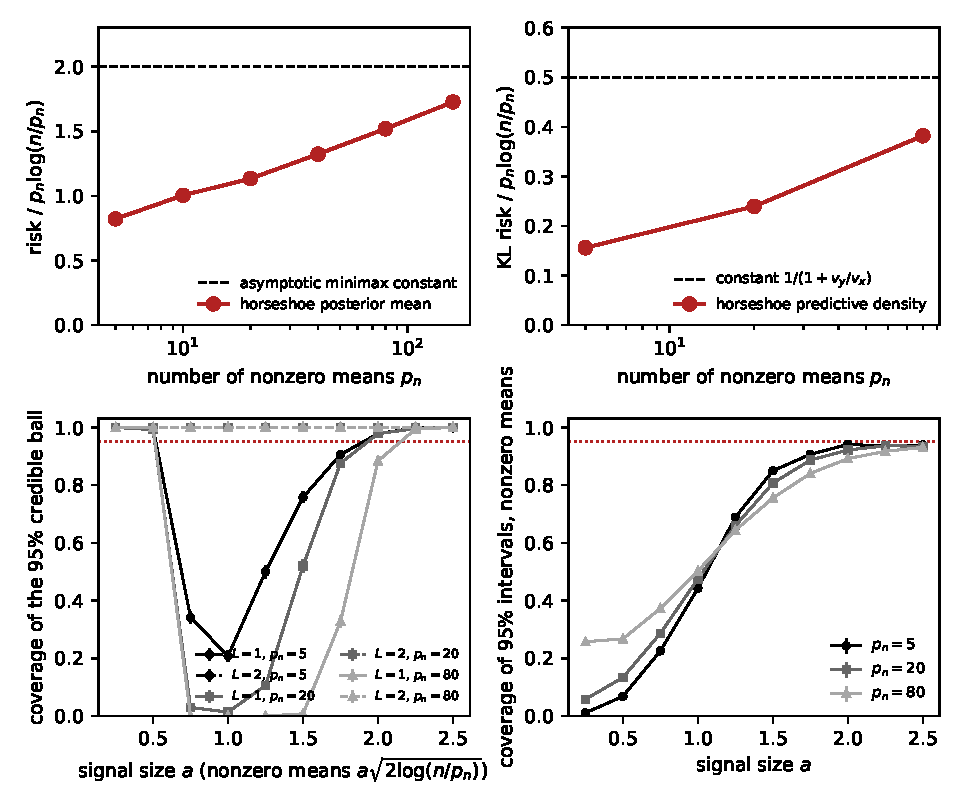
\includegraphics[width=\linewidth]{fig_hs_theory.pdf}
\caption{The horseshoe in the sparse normal means model, $n = 2{,}000$, 500 replications per point, with error bars of one Monte Carlo standard error. Top left: squared error risk of the posterior mean divided by $p_n\log(n/p_n)$, with the asymptotic minimax constant 2. Top right: Kullback and Leibler risk of the horseshoe predictive density, computed through the identity of Theorem~\ref{pg:thm:glx}, divided by $p_n\log(n/p_n)$, with the constant $1/2$ of the exact minimax risk (dashed). Bottom left: coverage of the 95 percent credible ball at its own radius ($L=1$, solid) and at twice it ($L=2$, dashed) against the signal size $a$, for $p_n = 5$, 20 and 80. Bottom right: coverage of central 95 percent posterior intervals for the nonzero means. The dotted lines mark 0.95.}
\label{pg:fig:hs}
\end{figure}

\section{Predictive densities}\label{pg:sec:pred}

Counterfactual prediction\index{counterfactual!prediction} is predictive density estimation\index{predictive density estimation|textbf}: the missing potential outcome of a treated unit, or the untreated outcome of a treated cohort after adoption, is a future observation to predict. The natural loss is the Kullback and Leibler divergence\index{Kullback Leibler divergence} between the true density of the future observation and the predictive density.

Let $X\sim N_n(\mu, v_x I)$ be observed and $Y\sim N_n(\mu, v_yI)$ be a future observation, independent given $\mu$. For a prior $\pi$ write $\hat p_\pi(y\mid x) = \int\phi(y;\mu,v_yI)\,\pi(\mu\mid x)\,d\mu$ for the Bayes predictive density, and
\[
R_{\mathrm{KL}}(\mu,\hat p_\pi) = \E_\mu\int\phi(y;\mu,v_yI)\log\frac{\phi(y;\mu,v_yI)}{\hat p_\pi(y\mid X)}\,dy .
\]
For $v>0$ let $\hat\mu_{\pi,v}$ be the posterior mean of $\mu$ based on $W\sim N_n(\mu,vI)$, with quadratic risk $R_Q(\mu,\hat\mu_{\pi,v}) = \E_\mu\lVert\hat\mu_{\pi,v}(W)-\mu\rVert^2$.

\begin{theorem}[Brown, George and Xu 2008, Theorem 1]\label{pg:thm:glx}
Let $\pi$ be a prior density on $\mu$ under which the marginal density of $X$ is finite everywhere, and let $R_{\mathrm{KL}}(\mu,\hat p_\pi)$\index{predictive density estimation} be finite. With $v_w = v_xv_y/(v_x+v_y)$,
\[
R_{\mathrm{KL}}(\mu,\hat p_\pi) = \frac12\int_{v_w}^{v_x}\frac{1}{v^2}\,R_Q(\mu,\hat\mu_{\pi,v})\,dv .
\]
\end{theorem}

Brown, George and Xu prove the identity in difference form, against the uniform prior, from Lemmas 2 and 3 of George, Liang and Xu (2006) and Stein's formula for quadratic risk; the form displayed follows because the uniform prior has $R_{\mathrm{KL}} = (n/2)\log(v_x/v_w)$ and the maximum likelihood estimator has quadratic risk $nv$. The identity links predictive risk to estimation risk at noise levels between that of the observed data, $v_x$, and that of the data augmented by the future observation, $v_w$. Priors with superharmonic marginals give predictive densities that dominate the uniform prior's and are minimax (George, Liang and Xu 2006).

\begin{corollary}[Predictive risk of the horseshoe]\label{pg:cor:hspred}
In the sparse normal means model with $v_x$ and $v_y$ fixed, as $n\to\infty$ with $p_n\to\infty$ and $p_n = o(n)$, let $\pi$ be the horseshoe prior\index{predictive density estimation!for the horseshoe|textbf} on $\mu$ with $\gscale = (p_n/n)^\alpha$ and $\alpha\ge1$, on the scale $\mu_i\mid\lambda_i\sim N(0,\lambda_i^2\gscale^2)$. Then
\[
\sup_{\mu\in\ell_0[p_n]}R_{\mathrm{KL}}(\mu,\hat p_\pi) \lesssim p_n\log(n/p_n)\,\log\Bigl(1 + \frac{v_x}{v_y}\Bigr).
\]
\end{corollary}
\begin{proof}
For $v\in[v_w,v_x]$, rescaling by $\sqrt v$ gives a unit variance model for $\mu/\sqrt v\in\ell_0[p_n]$ with $\tau_{\mathrm{g},v}=\gscale/\sqrt v=c_v(p_n/n)^\alpha$ and $c_v=v^{-1/2}\in[v_x^{-1/2},v_w^{-1/2}]$. Since $\alpha\ge1$, $\log(1/\tau_{\mathrm{g},v})=O(\log(n/p_n))$ and $n\tau_{\mathrm{g},v}\le c_vp_n$. Theorem~\ref{pg:thm:hs} therefore gives $R_Q(\mu,\hat\mu_{\pi,v})\lesssim v\,p_n\log(n/p_n)$ uniformly over $\mu\in\ell_0[p_n]$ and $v\in[v_w,v_x]$. Integrating with Theorem~\ref{pg:thm:glx} gives
\[
R_{\mathrm{KL}}(\mu,\hat p_\pi)\lesssim p_n\log(n/p_n)\int_{v_w}^{v_x}\frac{dv}{v}=p_n\log(n/p_n)\log\Bigl(1+\frac{v_x}{v_y}\Bigr).
\]
\end{proof}

Mukherjee and Johnstone (2015) compute the exact asymptotic minimax predictive risk, of order $p_n\log(n/p_n)$, and construct a prior that attains it. Zhai and Ro\v{c}kov\'a (2026) prove exact asymptotic minimaxity for the horseshoe predictive density with known sparsity. With an exponential hyperprior on $\gscale$ of rate $n$, it adapts to unknown sparsity when every nonzero mean exceeds $c\sqrt{2\log n}$ in noise units, $c>\sqrt6$ (their Theorem~3.1). The top right panel of Figure~\ref{pg:fig:hs} computes the Kullback and Leibler risk through Theorem~\ref{pg:thm:glx} with $v_x = v_y = 1$: divided by $p_n\log(n/p_n)$ it stays between \pgkmin\ and \pgkmax, against the constant $1/(1+v_y/v_x) = 1/2$ in the exact minimax risk of Mukherjee and Johnstone.

\section{Consequences for treatment effects}\label{pg:sec:causal}

\paragraph{Heterogeneous effects in a trial.} For $K$ prespecified, disjoint subgroups in a randomized trial, let $\hat\tau_k\sim N(\tau_k,\sigma^2)$ independently, where $\tau_k=\bar\tau+\delta_k$ with $p$ nonzero deviations. If $\bar\tau$ is known, $\hat\tau_k-\bar\tau$ is a sparse normal means problem. As $K\to\infty$ with $p\to\infty$ and $p=o(K)$, Theorems~\ref{pg:thm:hs} and \ref{pg:thm:adaptive} give posterior concentration\index{posterior contraction!for treatment effects|textbf} of $\delta$ at squared Euclidean rate $\sigma^2p\log(K/p)$ with the oracle scale, or $\sigma^2p\log K$ adaptively. Estimating $\bar\tau$ from the same data under a flat prior gives correlated projected noise and a mean that is not exactly sparse, so this rate remains heuristic. With known $\bar\tau$, shrinkage toward the common effect is minimax over the sparse class, with vanishing shrinkage of large subgroup effects\index{subgroup effect}.

\paragraph{Accounting functionals.} Any reported effect is a weighted sum $\psi_w = \sum_kw_k\tau_k$ of subgroup or cell effects.

\begin{corollary}\label{pg:cor:linear}
If the posterior of $\tau\in\R^K$ contracts around $\tau_0$ at rate $\varepsilon_K$ in Euclidean norm, then for any weight vector $w$ the posterior of $\psi_w = w^\top\tau$ contracts around $w^\top\tau_0$ at rate $\lVert w\rVert_2\,\varepsilon_K$.
\end{corollary}
\begin{proof}
$\lvert w^\top\tau - w^\top\tau_0\rvert\le\lVert w\rVert_2\lVert\tau-\tau_0\rVert_2$, so the event $\{\lvert\psi_w - w^\top\tau_0\rvert > M\lVert w\rVert_2\varepsilon_K\}$ is contained in $\{\lVert\tau-\tau_0\rVert_2 > M\varepsilon_K\}$.
\end{proof}

For a population average, $w_k$ is the share of subgroup $k$, so $\lVert w\rVert_2\le1$; equal shares improve the rate of the vector by the factor $\lVert w\rVert_2 = K^{-1/2}$.

\paragraph{Regularization induced confounding.} In the partially linear model with a flat prior on the treatment coefficient, Appendix~\ref{app:theory} expresses the shrinkage bias in that coefficient as a sum of the confounder coefficients' shrinkage errors, with weights from the treatment model. It derives the formula for a normal prior, but its first step, $\hat\tau = (T^\top T)^{-1}T^\top(Y - X\hat\beta)$ with $\hat\beta$ the posterior mean of the confounder coefficients, holds for any prior on them independent of the flat prior on $\tau$, the horseshoe included. When the confounders are orthogonal after the treatment is removed and the global and noise scales are held fixed, the posterior acts coordinatewise. Tail robustness then makes the shrinkage of a large coefficient, relative to its least squares estimate, of order $s_j^2/\lvert\beta_j\rvert$, where $s_j^2$ is the sampling variance of that estimate, so large confounders induce vanishing bias. The bias comes from confounders of intermediate size, up to about the detection boundary, and these are largely the coordinates for which the marginal credible intervals of Section~\ref{pg:sec:hs} fail. A learned global or noise scale couples the coefficients through its posterior, and correlated confounders couple them through the likelihood; in either case the posterior mean of a large coefficient also moves with the shrinkage of the others, and this account is a heuristic. Heuristically, for a normal prior and with the propensity known (Appendix~\ref{app:theory}), the propensity covariate of Chapter~\ref{ch:horseshoe} removes the first order part of this term by not shrinking in the direction of the propensity score.

\section{Difference in differences}\label{pg:sec:did}

The horseshoe difference in differences\index{difference in differences!posterior guarantees|textbf} estimator of Chapter~\ref{ch:did} writes the effect in cohort $g$ at event time $e$ as $\tau_{g,e} = \theta_e + u_{g,e}$, a common event path plus sparse cohort deviations, and allows sparse unit departures $\delta_i$ from parallel trends.

\begin{corollary}[Cohort deviations, oracle event path]\label{pg:cor:did}
Suppose the cell estimates satisfy $Z_{g,e} = \theta_e + u_{g,e} + \varepsilon_{g,e}$ for $g = 1,\dots,G$ and $e = 1,\dots,E$, with $\varepsilon_{g,e}\sim N(0, \sigma^2/m)$ independent, $m$ the number of units per cell, the event path $\theta$ known, and at most $s$ nonzero deviations among the $GE$ cells, as $GE\to\infty$ with $s\to\infty$ and $s = o(GE)$. With a horseshoe prior on $u$, the posterior of $u$ contracts in Euclidean norm at rate $\varepsilon_{GE}$, where
\[
\varepsilon_{GE}^2 = \frac{\sigma^2}{m}\,s\log\frac{GE}{s},
\]
which is the minimax rate over $s$ sparse deviations when the global scale is set at the oracle value $\gscale = (s/GE)^\alpha$ with $\alpha\ge1$; $\varepsilon_{GE}^2$ becomes $(\sigma^2/m)\,s\log(GE)$ when the scale is chosen adaptively under the conditions of Theorem~\ref{pg:thm:adaptive}, and by Corollary~\ref{pg:cor:linear} the posterior of the effect on the treated, $\sum_{g,e}w_{g,e}\tau_{g,e}$ with weights proportional to cell sizes, contracts at rate $\lVert w\rVert_2\,\varepsilon_{GE}$; since every cell has $m$ units, $w_{g,e} = 1/(GE)$ and $\lVert w\rVert_2 = (GE)^{-1/2}$.
\end{corollary}
\begin{proof}
Given $\theta$, the observations $Z_{g,e}-\theta_e$ form a sequence model with $n = GE$, noise variance $\sigma^2/m$ and an $s$ sparse mean, so Theorems~\ref{pg:thm:hs} and \ref{pg:thm:adaptive} apply after rescaling by $\sigma/\sqrt m$, and the minimax lower bound of Donoho, Johnstone, Hoch and Stern applies to the same class. The second claim is Corollary~\ref{pg:cor:linear}.
\end{proof}

When the event path is estimated, an error in $\hat\theta_e$ is shared by all $G$ cohorts at event time $e$. If each $\hat\theta_e$ has mean squared error of order $\sigma^2/(mG)$, as when few of the cohorts deviate at event time $e$, this adds a squared error of order $G\cdot E\cdot\sigma^2/(mG) = E\sigma^2/m$ to the cell effects, of smaller order than $\varepsilon_{GE}^2$ when $s\log(GE/s)\gg E$. Total sparsity, $s=o(GE)$, does not give that error bound, since it allows every cohort to deviate at the same event time. A full proof for the joint posterior of $(\theta,u)$ would need a condition separating the common path from the deviations, such as a restricted eigenvalue condition analogous to the compatibility conditions of high dimensional regression; we leave it open, with the corresponding result for unit departures. The simulation of Chapter~\ref{ch:did}, with a flat event path and horseshoe deviations, gives coverage close to nominal, although the corollary concerns the rate and not coverage.

\paragraph{Parallel trends and prediction.} With the common trend known and horseshoe unit departures $\delta_i$ observed with independent noise, predicting a treated unit's untreated path is an idealized sparse predictive density problem. Corollary~\ref{pg:cor:hspred} would bound its Kullback and Leibler risk by a multiple of $p\log(N/p)\log(1+v_x/v_y)$ when at most $p$ of the $N$ units depart from parallel trends, $v_x$ is the noise variance of the estimated departures and $v_y$ that of a future outcome. The parallel trends assumption becomes a sparsity assumption about departures, and the price of not knowing which units depart is the logarithmic factor.

\section{Groups, scales and stability}\label{pg:sec:groups}

This section proves the guarantees of Chapter~\ref{ch:groups}\index{group action!posterior guarantees|textbf}; the other proofs of that chapter are in Appendix~\ref{app:groupsproofs}.

\begin{proof}[Proof of Theorem~\ref{gr:thm:recon}, part (b)]
On the chart scale, $z_i=h(Y_i)-h(\gamma_i)=\theta+\varepsilon_i$ for the $n_1$ treated units, with $\theta=\psi(g)$ and independent errors of density $f$: a location model, a transformation model for $G\cong\R$ acting by $z\mapsto z+c$. Let $\hat g$ be equivariant and $\hat\theta=\psi(\hat g)$, so that $\hat\theta(z+c)=\hat\theta(z)+c$, and let $a=(z_i-\hat\theta)_i$ be the maximal invariant. Since $z_i=\hat\theta+a_i$, the Jacobian of the change from $z$ to $(\hat\theta,a)$ depends only on $a$, so the conditional sampling density of $\hat\theta$ given $a$ is
\[
q(\hat\theta-\theta\mid a)=c_1(a)\prod_if(\hat\theta+a_i-\theta),
\]
with $c_1(a)^{-1}=\int\prod_if(t+a_i)\,dt$. The right Haar measure on $\R$ is Lebesgue measure, so the posterior density of $\theta$ is $c_1(a)\prod_if(\hat\theta+a_i-\theta)$ (substitute $t=\hat\theta-\theta$ in the normalizer). Hence the posterior law of $\hat\theta-\theta$ and its conditional sampling law given $a$ coincide. A set $\{\theta:\theta-\hat\theta\in A(a)\}$ of posterior probability $1-\alpha$ therefore has coverage $1-\alpha$, conditionally on $a$ and unconditionally. The location case is due to Fisher (1934) and Pitman (1939), the group version to Fraser (1961), and Hora and Buehler (1966) give the confidence property.

For a general group $G$ acting on the observations the same argument runs as follows. Let $z=ge$ with $e$ drawn from a fixed law, and let $\mu$ be a measure on the sample space that is relatively invariant under $G$, $\mu(kB)=\chi(k)\mu(B)$ with $\chi$ a homomorphism to $(\R^{+},\times)$, such that $e$ has density $p_e$ with respect to $\mu$. Then $z$ has density $\chi(g)^{-1}p_e(g^{-1}z)$. Let $\hat g(z)$ be equivariant, $\hat g(kz)=k\hat g(z)$, put $z_a=\hat g(z)^{-1}z$, which depends on $z$ through the maximal invariant $a$ only, and take the pivot $q=g^{-1}\hat g$. In the coordinates $(\hat g,a)$ the measure $\mu$ is $\chi(\hat g)\,\nu_L(d\hat g)\,\kappa(da)$ with $\nu_L$ the left Haar measure, so the density of $(\hat g,a)$ with respect to $\nu_L\otimes\kappa$ is $\chi(g)^{-1}\chi(\hat g)\,p_e(g^{-1}\hat gz_a)=\chi(q)\,p_e(qz_a)$, and by left invariance of $\nu_L$ the pivot $q$ has, given $a$, a density proportional to $\chi(q)p_e(qz_a)$ with respect to $\nu_L(dq)$ whatever $g$ is. The posterior under the right Haar prior $\nu_R$ is proportional to $\chi(g)^{-1}p_e(g^{-1}\hat gz_a)\,\nu_R(dg)$. Substitute $g=\hat gq^{-1}$: inversion turns $\nu_R$ into $\nu_L$, left translation by $\hat g$ multiplies it by a constant that does not involve $q$, and $\chi(g)^{-1}=\chi(\hat g)^{-1}\chi(q)$, so the posterior density of $q$ with respect to $\nu_L(dq)$ is proportional to $\chi(q)p_e(qz_a)$, the conditional sampling density of $q$ given $a$. A left Haar prior would leave a factor that depends on $q$, which is why it fails. The conclusion is as before: a set $\{g:g^{-1}\hat g\in A(a)\}$ of posterior probability $1-\alpha$ has coverage exactly $1-\alpha$, conditionally on $a$ and unconditionally.
\end{proof}

\begin{proof}[Proof of Theorem~\ref{gr:thm:select}]
Write $\ell_n$ for the log likelihood, $\hat\ell_G=\max_{F\in\mathcal S_G}\ell_n(F)$ and $W_n^G=\KL_w(L_n\,\|\,\mathcal S_G)$. Since cell $(x,t)$ holds $nw_{x,t}$ independent draws, $\ell_n(F)=-n\sum_{x,t}w_{x,t}\{\mathrm{Ent}(L_{n,x,t})+\KL(L_{n,x,t}\,\|\,F_{x,t})\}$ with $\mathrm{Ent}$ the entropy; maximizing $\ell_n$ over $\mathcal S_G$ therefore minimizes $\KL_w(L_n\,\|\,F)$, and
\[
\hat\ell_G-\hat\ell_H=n\,(W_n^H-W_n^G)
\]
exactly, because the entropy term is common to the two models. For each model, Laplace's method under the assumed smooth positive prior and nonsingular Hessian at the projection gives the marginal likelihood $m_G$ as $\log m_G=\hat\ell_G-\tfrac12d_G\log n+O_p(1)$, whether or not the model contains $F^{\circ}$. With $\pi_G$ the prior probability of model $G$, $\Pi(\mathcal S_G\mid\text{data})\propto\pi_Gm_G$, so
\[
\log\frac{\Pi(\mathcal S_G\mid\text{data})}{\Pi(\mathcal S_H\mid\text{data})}=n\,(W_n^H-W_n^G)-\tfrac12(d_G-d_H)\log n+O_p(1).
\]
By the strong law $L_n\to F^{\circ}$ almost surely, and $W_n^G\to D_G$ because $F\mapsto\KL_w(F\,\|\,\mathcal S_G)$ is continuous at $F^{\circ}$ (the projection is unique and interior). The Laplace remainders depend on the data through $L_n$ only, so they are $O(1)$ almost surely, which gives the almost sure limit. For the expansion, when $F^{\circ}\notin\mathcal S_G$ the statistic $W_n^G$ is a smooth function of $L_n$ near $F^{\circ}$ and $L_n-F^{\circ}=O_p(n^{-1/2})$, so $n(W_n^G-D_G)=O_p(\sqrt n)$ by the delta method. When $F^{\circ}\in\mathcal S_G$, $nW_n^G$ is half the deviance of $G$ against the saturated model and is $O_p(1)$. Hence the fluctuation of the log odds about $n(D_H-D_G)-\frac12(d_G-d_H)\log n$ is $O_p(\sqrt n)$, and $O_p(1)$ when both models contain $F^{\circ}$.
\end{proof}

\begin{proof}[Proof of Corollary~\ref{gr:cor:select}]
All three parts are read off the last display of the preceding proof. (i) Since $D_{\mathrm{sat}}=0$, the unique group $G$ with $D_G=0$ has log odds $nD_H+O_p(\sqrt n)\to\infty$ against every other group $H$, and $\tfrac12(d_{\mathrm{sat}}-d_G)\log n+O_p(1)\to\infty$ against the saturated model, which also contains $F^{\circ}$, because $d_G<d_{\mathrm{sat}}$. So its posterior probability tends to one, with the stated exponential and polynomial rates. (ii) The latter log odds give order $n^{(d_{\mathrm{sat}}-d_G)/2}$ under the smooth positive prior, with $d_{\mathrm{sat}}-d_G=2J-(J+1)=J-1$. (iii) If no group contains $F^{\circ}$, let $G$ attain $D_{\min}=\min_HD_H>0$. The saturated model's log odds against $G$ are $nD_{\min}-\tfrac12(d_{\mathrm{sat}}-d_G)\log n+O_p(\sqrt n)\to\infty$, and likewise against every other group, so its posterior probability tends to one. The leading order weights $e^{-nD-\frac12d\log n}$, which leave out the $O_p(\sqrt n)$ fluctuation, cross where $nD_{\min}=\tfrac12(d_{\mathrm{sat}}-d_G)\log n$.
\end{proof}

\begin{proof}[Proof of Proposition~\ref{gr:prop:hstest}]
Write $\sigma_J^2=\sigma^2J/n$ for the variance of each $\hat\psi_j$, let $U$ be a $J\times(J-1)$ matrix whose orthonormal columns span the contrasts, the vectors orthogonal to $(1,\dots,1)$, and put $z=U^{\top}\hat\psi/\sigma_J$, so that $|z|^2=\sum_j(\hat\psi_j-\bar{\hat\psi})^2/\sigma_J^2$ with $\bar{\hat\psi}$ the mean of the $\hat\psi_j$. Given the scales $\lambda=(\lambda_j)$ and $\gscale$, $\hat\psi\sim N(\psi\mathbf 1,\sigma_J^2I+\gscale^2\Lambda^2)$ with $\Lambda=\operatorname{diag}(\lambda_j)$. A flat prior on $\psi$ integrates the likelihood to the density of the contrasts $U^{\top}\hat\psi\sim N\{0,\sigma_J^2(I+u^2B)\}$ times $J^{-1/2}$, where $u=\gscale/\sigma_J$ and $B=U^{\top}\Lambda^2U$, and the factor $J^{-1/2}$ is the same under stability, $u=0$. So the ratio of the integrated likelihood of the alternative to that of stability, at $(u,\lambda)$, is
\[
R(u,\lambda,z)=|I+u^2B|^{-1/2}\exp\Bigl\{\tfrac12z^{\top}u^2B(I+u^2B)^{-1}z\Bigr\},
\]
which depends on the data through $z$ alone, and $\mathrm{BF}_{10}=\int_0^\infty r(u)\,p(\sigma_Ju)\,\sigma_J\,du$ with $r(u)=\E_\lambda R(u,\lambda,z)$ and $p$ the prior density of $\gscale$. Since $u^2B(I+u^2B)^{-1}\preceq I$ and $|I+u^2B|\ge1$, $R\le e^{|z|^2/2}$ for every $u$ and $\lambda$. Under stability $z\sim N(0,I_{J-1})$ whatever $n$ and $\sigma$.

(i) Take prior A, $p(\gscale)=2/\{\pi(1+\gscale^2)\}$, so that $p(\sigma_Ju)\le2/\pi$ and $p(\sigma_Ju)\to2/\pi$ as $n\to\infty$ for each $u$. Let $J\ge3$; it remains to show that $r$ is integrable, so that dominated convergence applies. Since $UU^{\top}=I-J^{-1}\mathbf 1\mathbf 1^{\top}$, Sylvester's identity and the matrix determinant lemma give
\[
|I+u^2B|=\frac1J\sum_{k=1}^J\prod_{j\ne k}(1+u^2\lambda_j^2)\ge\frac1J\prod_{j=1}^{J-1}(1+u^2\lambda_j^2).
\]
With $m(u)=\E(1+u^2\lambda^2)^{-1/2}$ for a half Cauchy $\lambda$, independence of the local scales yields $r(u)\le e^{|z|^2/2}\sqrt J\,m(u)^{J-1}$, and splitting the integral defining $m$ at $\lambda=1$ gives $m(u)\le(2/\pi)(3/2+\log u)/u$ for $u\ge1$. Since $J-1\ge2$, $(\log u/u)^{J-1}$ is integrable at infinity, and $r(u)\le e^{|z|^2/2}$ near zero, so $0<\int_0^\infty r(u)\,du<\infty$. By dominated convergence $\sigma_J^{-1}\mathrm{BF}_{10}\to(2/\pi)\int_0^\infty r(u)\,du$, so $\sigma_J\mathrm{BF}_{01}$ converges in distribution to the positive finite random variable $\pi/\{2\int_0^\infty r(u)\,du\}$, which says $\mathrm{BF}_{01}\asymp_p\sqrt n/\sigma$ for fixed $J$. For $J=2$ there is one contrast and $B=(\lambda_1^2+\lambda_2^2)/2$. Then $u\,r(u)\to c(z)=e^{z^2/2}\E B^{-1/2}$ as $u\to\infty$ by dominated convergence, since $u(1+u^2B)^{-1/2}\le B^{-1/2}$ and $\E B^{-1/2}<\infty$ (polar coordinates in $(\lambda_1,\lambda_2)$, whose density is bounded). Splitting the integral at $u=1$ and writing $\varepsilon=\sigma_J$, $\int_0^\infty r(u)\,p(\varepsilon u)\,du=\{1+o(1)\}(2/\pi)\,c(z)\log(1/\varepsilon)$, because $\int_1^\infty u^{-1}(1+\varepsilon^2u^2)^{-1}du=\log(1/\varepsilon)+O(1)$ and the part over $[0,1]$ is at most $e^{z^2/2}$. So $\mathrm{BF}_{10}=\{1+o(1)\}\,\sigma_J\,c(z)\log n/\pi$, using $\log(1/\sigma_J)=\tfrac12\log n+O(1)$, and $\mathrm{BF}_{01}\asymp_p\sqrt n/(\sigma\log n)$. For $J=1$ there is no contrast and stability cannot be tested.

(ii) Write $\hat\psi_j=\psi+\eta_j+\sigma_J\xi_j$ with $\xi_j$ standard normal. Then $z=U^{\top}\eta/\sigma_J+\xi'$ with $\xi'\sim N(0,I_{J-1})$ and $|U^{\top}\eta|^2=\sum_j(\eta_j-\bar\eta)^2=:\Delta^2>0$, so $|z|^2=\{1+o_p(1)\}\Delta^2/\sigma_J^2=\{1+o_p(1)\}\,n\Delta^2/(J\sigma^2)$. Prior A integrates to one, so $R\le e^{|z|^2/2}$ gives $\log\mathrm{BF}_{10}\le|z|^2/2$. For the lower bound fix $\delta\in(0,1)$ and $a\in(0,1)$, and choose $u_0$ with $u_0^2a^2\ge1/\delta$. On the event $\{\lambda_j\in[a,1]\text{ for all }j\}$, which has positive prior probability $\varpi_a$ under the half Cauchy law, every eigenvalue of $B$ lies in $[a^2,1]$, because $B$ is the compression of $\Lambda^2$ to a subspace. For $u\in[u_0,2u_0]$ on that event, $z^{\top}u^2B(I+u^2B)^{-1}z\ge(1-\delta)|z|^2$ and $|I+u^2B|\le(1+4u_0^2)^{J-1}$, so $R\ge(1+4u_0^2)^{-(J-1)/2}e^{(1-\delta)|z|^2/2}$. Hence
\[
\mathrm{BF}_{10}\ge\varpi_a(1+4u_0^2)^{-(J-1)/2}e^{(1-\delta)|z|^2/2}\int_{\sigma_Ju_0}^{2\sigma_Ju_0}p(\gscale)\,d\gscale,
\]
and the last integral is at least $c\,\sigma_J$ for a constant $c>0$ and $n$ large. So $\log\mathrm{BF}_{10}\ge(1-\delta)|z|^2/2-O(\log n)$, and $\log n=o(|z|^2)$ because $|z|^2\asymp n$. Since $\delta$ is arbitrary, $\log\mathrm{BF}_{10}=\{1+o_p(1)\}\,|z|^2/2=\{1+o_p(1)\}\,\dfrac{n}{2J\sigma^2}\sum_j(\eta_j-\bar\eta)^2$.

(iii) With $\psi$ known, dividing $\hat\psi_j-\psi=\eta_j+\sigma_J\xi_j$ by $\sigma_J$ gives the sparse normal means model with unit noise and, under prior B, the horseshoe with global scale $\gscale/\sigma_J$ on a half Cauchy law truncated to $[1/J,1]$. Van der Pas, Szab\'o and van der Vaart (2017a, Theorem~3.7 and Example~3.3) give squared error contraction for $\eta$ at rate $(\sigma^2J/n)\,s\log J$ for $s=o(J)$ and $s\ge C\log J$, of the order of the minimax rate $(\sigma^2J/n)\,s\log(J/s)$ whenever $s\le J^{1-c}$ for some $c>0$. For a deterministic global scale $(s/J)^{\alpha}$ in noise units, with $\alpha\ge1$, van der Pas, Kleijn and van der Vaart (2014) give the minimax rate. Both theorems need $s\to\infty$ and $s=o(J)$, and neither covers an unknown common level, which is why (iii) takes $\psi$ known.

(iv) Under prior B, $\mathrm{BF}_{10}=\int_{1/J}^{1}r(u)p_B(u)\,du$, where $p_B$ is the normalized half Cauchy density on $[1/J,1]$. Thus $\mathrm{BF}_{01}=1/\mathrm{BF}_{10}$ depends on the data through $z$ alone, whose law under stability is independent of $n$ and $\sigma$.
\end{proof}

\begin{proof}[Proof of Proposition~\ref{gr:prop:effect}]
Let $\ell_p(\psi)$ be the log likelihood maximized over the baselines for fixed $\psi$. With $J_G$ defined at the empirical law, $nJ_G(\psi)=\hat\ell_G-\ell_p(\psi)$ by the identity for $\ell_n$ in the proof of Theorem~\ref{gr:thm:select}. The posterior density of $\psi$ is the integral of the likelihood and the prior over the baselines. By Laplace's method it equals
\[
\exp\{\ell_p(\psi)\}\,(2\pi/n)^{(d_G-1)/2}s(\psi)\{1+O_p(n^{-1})\},
\]
where $s$ is the prior density at the conditional maximum divided by the square root of the determinant of the baseline information, smooth and bounded above and below on compact sets. So the density is proportional to $e^{-nJ_G(\psi)}s(\psi)$. By the regularity assumed in the statement, $J_G$ is smooth, vanishes only at $\hat\psi$, increases away from it with $J_G'(\psi)\neq0$ for $\psi\neq\hat\psi$, and has $J_G''(\hat\psi)>0$, the positive information about the effect. Integrating over a bounded $A$ gives $e^{-n\inf_AJ_G}$ times a factor polynomial in $n$, and the normalizing constant is of order $n^{-1/2}$ because $J_G$ has a nondegenerate minimum at $\hat\psi$. An unbounded $A$, such as $\{\psi\le0\}$, needs a bound on its tail, and the profile likelihood gives one: the likelihood at any $(\psi,\gamma)$ is at most $e^{\ell_p(\psi)}=e^{\hat\ell_G-nJ_G(\psi)}$, so before normalization the part of $A$ outside a compact set contributes at most $e^{\hat\ell_G-n\inf_AJ_G}$, since the prior has total mass one, against a marginal likelihood of $e^{\hat\ell_G}$ times a factor polynomial in $n$, and the rate is unchanged. This is the first statement.

For the second, put $v(\psi)=\operatorname{sign}(\psi-\hat\psi)\sqrt{2J_G(\psi)}$, a smooth increasing coordinate near $\hat\psi$ with $r(\psi)=\sqrt n\,v(\psi)$. In it the posterior density is proportional to $e^{-nv^2/2}m(v)$ with $m(v)=s(\psi)\,d\psi/dv$ smooth and positive. With $v_0=v(\psi_0)$, the expansion $m(v)=m(0)+m'(0)v+O(v^2)$ gives
\[
\Pi(\psi\le\psi_0\mid\text{data})=\Phi(r(\psi_0))-\frac{m'(0)}{m(0)}\,n^{-1/2}\varphi(r(\psi_0))+O(n^{-1}),
\]
with $\varphi$ the standard normal density, when $r(\psi_0)=O(1)$, that is, when $\psi_0-\hat\psi=O(n^{-1/2})$, and the relative error of $\Phi(r(\psi_0))$ is then $O(n^{-1/2})$. 

For $\psi_0<\hat\psi$ and $v_0<0$ bounded away from zero as $n$ grows, $J_G'\neq0$ off $\hat\psi$ makes $v$ a smooth coordinate on $[\psi_0,\hat\psi]$. With $m$ smooth and positive, Laplace's method at the endpoint and minimum gives
\begin{align*}
\int_{-\infty}^{v_0}e^{-nv^2/2}m(v)\,dv&=\frac{m(v_0)e^{-nv_0^2/2}}{n|v_0|}\{1+O(n^{-1})\},\\
\int e^{-nv^2/2}m(v)\,dv&=m(0)\sqrt{\frac{2\pi}n}\{1+O(n^{-1})\},
\end{align*}
while $\Phi(r(\psi_0))\sim e^{-nv_0^2/2}/(\sqrt{2\pi n}\,|v_0|)$. The ratio of the posterior probability to $\Phi(r(\psi_0))$ therefore tends to $m(v_0)/m(0)$, which in terms of the original quantities is
\[
\frac{s(\psi_0)}{s(\hat\psi)}\,\frac{\sqrt{2J_G''(\hat\psi)J_G(\psi_0)}}{|J_G'(\psi_0)|}.
\]
The ratio equals one exactly when $m(v_0)=m(0)$, as it does for every $\psi_0$ under a prior flat in the signed root coordinate, for example when $s$ is constant and $J_G$ quadratic. In general the relative error for fixed $\psi_0$ is $O(1)$, not $o(1)$.
\end{proof}



\chapter{Solutions to the Exercises}\label{app:solutions}



\section*{Chapter~\ref{ch:predictive}: Causal Questions}

\paragraph{Exercise~\ref{ex:ch01:1}.} Under complete randomization with $n_1$ treated and $n_0$ controls, each unit is treated with probability $n_1/n$. The treated sample mean $\bar Y_1 = n_1^{-1}\sum_i T_i Y_i(1)$ has expectation $n_1^{-1}\sum_i (n_1/n)Y_i(1) = \bar Y(1)$, the finite population mean of treated potential outcomes, and similarly for controls, so $\bar Y_1 - \bar Y_0$ is unbiased for $\tau_{\mathrm{fp}}$. For the variance write $\bar Y_1 - \bar Y_0 = \sum_i T_ic_i - \sum_i Y_i(0)/n_0$ with $c_i = Y_i(1)/n_1 + Y_i(0)/n_0$. Under complete randomization $\mathrm{Var}(T_i) = n_1n_0/n^2$ and $\mathrm{Cov}(T_i, T_j) = -n_1n_0/\{n^2(n-1)\}$ for $i \neq j$, so $\mathrm{Var}(\sum_i T_ic_i) = (n_1n_0/n)S_c^2$ with $S_c^2 = \sum_i(c_i - \bar c)^2/(n-1)$. Expanding $S_c^2$ and using $S_\tau^2 = S_1^2 + S_0^2 - 2S_{10}$ gives
\[
\mathrm{Var}(\bar Y_1 - \bar Y_0) = \frac{S_1^2}{n_1} + \frac{S_0^2}{n_0} - \frac{S_{\tau}^2}{n},
\]
where $S_t^2$ is the finite population variance of $Y_i(t)$, $S_{10}$ the finite population covariance of $Y_i(1)$ and $Y_i(0)$, and $S_\tau^2$ the variance of the unit effects, all with divisor $n - 1$. The last term is not estimable, because it involves both potential outcomes of the same units. The treated units are a simple random sample of the $n$ units, so the sample variance $s_1^2$ of the observed treated outcomes, with divisor $n_1 - 1$, has expectation $S_1^2$, and likewise $s_0^2$ has expectation $S_0^2$. Neyman's estimator $s_1^2/n_1 + s_0^2/n_0$ therefore has expectation $\mathrm{Var}(\bar Y_1 - \bar Y_0) + S_\tau^2/n$: it is conservative, and exact when every unit has the same effect.

\paragraph{Exercise~\ref{ex:ch01:2}.} Write the observed outcome as $Y = \alpha + \tau T + \beta^\top X + \gamma^\top X T + \varepsilon$, with coefficient vector $\vartheta = (\alpha, \tau, \beta, \gamma)$ of dimension $d = 2p + 2$, a flat prior on $\vartheta$ and Jeffreys' prior on $\sigma^2$. Let $Z$ be the design matrix, $\hat\vartheta$ the least squares estimate and $s^2$ the residual variance on $\nu = n - d$ degrees of freedom. The posterior of $\vartheta$ is multivariate Student $t$ with location $\hat\vartheta$ and scale matrix $s^2(Z^\top Z)^{-1}$. Since $\tau(x) = \tau + \gamma^\top x$ is linear in $x$, the average effect for the covariate law $Q$ is
\[
\tau_Q = \int \tau(x)\,Q(dx) = \tau + \gamma^\top m_Q = a^\top\vartheta,
\]
with $m_Q = \int x\,Q(dx)$ and $a = (0, 1, 0_p, m_Q)$, a fixed linear combination of the coefficients. Its posterior is a scaled Student $t$ with $\nu$ degrees of freedom, location $\hat\tau + \hat\gamma^\top m_Q$ and squared scale $s^2 a^\top (Z^\top Z)^{-1} a$, and for $\nu > 2$ its variance is
\[
\frac{\nu s^2}{\nu - 2}\bigl(B_{\tau\tau} + 2\,m_Q^\top B_{\gamma\tau} + m_Q^\top B_{\gamma\gamma}\,m_Q\bigr),
\]
where $B$ is the block of $(Z^\top Z)^{-1}$ belonging to $(\tau, \gamma)$. Of $Q$ only $m_Q$ appears. Two populations with the same mean of $X$ and very different spreads have the same posterior for the average effect, and without the interaction even $m_Q$ drops out, as Section~\ref{sec:firstexample} says.

\paragraph{Exercise~\ref{ex:ch01:3}.} Given $\theta$, the missing outcome of unit $i$ is normal with variance $\sigma_{1-T_i}^2(1-\rho^2)$, so $\mathrm{Var}(\tau_{\mathrm{fp}}\mid\theta,\text{data})=n^{-2}\sum_i\sigma_{1-T_i}^2(1-\rho^2)$ decreases with $|\rho|$ and vanishes at $\rho=\pm1$. In the two arm model without covariates, with known variances and flat priors, $\mu_t\mid\text{data}\sim N(\bar y_t,\sigma_t^2/n_t)$ independently, giving $\mathrm{Var}(\tau\mid\text{data})=\sigma_1^2/n_1+\sigma_0^2/n_0$. The imputed outcome of a treated unit with observed value $y_i$ has mean $\mu_0+\rho(\sigma_0/\sigma_1)(y_i-\mu_1)$, and that of a control has mean $\mu_1+\rho(\sigma_1/\sigma_0)(y_i-\mu_0)$. The conditional mean of $n\tau_{\mathrm{fp}}$ is therefore $(n_0+\rho n_1\sigma_0/\sigma_1)\mu_1-(n_1+\rho n_0\sigma_1/\sigma_0)\mu_0$ plus data terms. Total variance gives
\[
\begin{split}
n^2\mathrm{Var}(\tau_{\mathrm{fp}}\mid\text{data})={}&(n_0+\rho n_1\sigma_0/\sigma_1)^2\frac{\sigma_1^2}{n_1}+(n_1+\rho n_0\sigma_1/\sigma_0)^2\frac{\sigma_0^2}{n_0}\\
&+(1-\rho^2)(n_1\sigma_0^2+n_0\sigma_1^2).
\end{split}
\]
The $\rho^2$ terms cancel, leaving
\[
\mathrm{Var}(\tau_{\mathrm{fp}}\mid\text{data})=\mathrm{Var}(\tau\mid\text{data})-\frac{\sigma_1^2+\sigma_0^2-2\rho\sigma_1\sigma_0}{n}.
\]
The subtracted term is the variance of the unit effects divided by $n$, the Bayesian twin of the $S_\tau^2/n$ term of Exercise~\ref{ex:ch01:1}. Thus $\tau_{\mathrm{fp}}$ has no greater posterior variance than $\tau$, with equality only for constant effects: $\rho=1$ and $\sigma_1=\sigma_0$, when Neyman's estimator is exact. For $n_1=n_0=1$, $\sigma_1=\sigma_0=1$ and $\rho=0$, the variances are 1 and 2.

\paragraph{Exercise~\ref{ex:ch01:4}.} Draw both balls without replacement from an urn containing $0$ and $1$. The pair $(Z_1,Z_2)$ is $(0,1)$ or $(1,0)$ with probability $1/2$ each, so it is exchangeable, with covariance $-1/4$. A mixture of independent and identically distributed sequences has $\mathrm{Cov}(Z_1,Z_2)=\mathrm{Var}\{\E(Z_1\mid\theta)\}\geq0$, ruling out such a representation. For the first $k$ of $n$ draws the total variation distance from sampling with replacement is at most $k(k-1)/(2n)$: a repeated index has at most this probability, and conditional on no repeat the laws agree. Finite exchangeable sequences are mixtures over urns, giving the approximation of Diaconis and Freedman (1980). The approximation suffices in Section~\ref{sec:exchangeability}, where $k^2$ is small relative to $n$. For a target averaging all $n$ units, $k=n$ makes the bound uninformative, and the target is the mean of the urn itself and not a parameter of an infinite mixture.

\paragraph{Exercise~\ref{ex:ch01:6}.} In a two person household let $T_i=1$ mean vaccinated and $Y_i=1$ mean infected. Suppose infection enters only when neither is vaccinated:
\[
Y_i(t_1,t_2)=\one\{t_1=t_2=0\},\qquad Y_i=Y_i(T_1,T_2),\quad i=1,2.
\]
Each unit has four potential outcomes. The stable unit treatment value assumption requires $Y_1(t_1,0)=Y_1(t_1,1)$, which at $t_1=0$ says $1=0$. The effect must therefore specify the other unit's treatment: $\tau_1(t_2)=Y_1(1,t_2)-Y_1(0,t_2)$ is $-1$ at $t_2=0$ and $0$ at $t_2=1$, and likewise for unit 2. If unit 2 is vaccinated with probability $q$, averaging gives $-(1-q)$, which depends on the assignment law. Nor do these effects add to a campaign's effect: vaccinating both reduces infections from 2 to 0, while the two effects measured with the other unit vaccinated sum to 0.

\paragraph{Exercise~\ref{ex:ch01:7}.} Write $V(\delta)$ for the value net of cost. Under ignorability and given $\theta$, $\mu_1(x) - \mu_0(x) = \tau + \gamma^\top x$, and $\mu_0(x) = \alpha + \beta^\top x$ does not depend on the policy, so
\[
V(\delta) = \int \mu_0(x)\,Q(dx) + \int \delta(x)\,(\tau + \gamma^\top x - c)\,Q(dx).
\]
Averaging over the posterior, the first term does not involve $\delta$ and the second becomes $\int \delta(x)\,g(x)\,Q(dx)$ with $g(x) = \E(\tau + \gamma^\top x \mid \text{data}) - c$. Since $\delta(x) \in \{0, 1\}$, this is largest when $\delta(x) = 1$ wherever $g(x) > 0$ and $\delta(x) = 0$ wherever $g(x) < 0$, and ties do not matter. That is $\delta^\ast$. For any $\delta$,
\begin{align*}
V(\delta^\ast) - V(\delta) &= \int \{\delta^\ast(x) - \delta(x)\}(\tau + \gamma^\top x - c)\,Q(dx)\\
&= w(\tau - c) + u^\top\gamma,
\end{align*}
with $w = \int (\delta^\ast - \delta)\,dQ$ and $u = \int (\delta^\ast - \delta)\,x\,Q(dx)$ fixed once the data are given, so the difference is affine in $(\tau, \gamma)$, with constant term $-cw$. Take $\delta \equiv 0$. Then $w = p_\ast$ is the share of $Q$ that $\delta^\ast$ treats, $u = p_\ast\,m_\ast$ with $m_\ast$ the mean of $X$ under $Q$ among the treated, and $D = V(\delta^\ast) - V(0) = p_\ast(\tau + \gamma^\top m_\ast - c)$. If $(\tau, \gamma)$ has a normal posterior with mean $(\hat\tau, \hat\gamma)$ and covariance $\Sigma$, and $p_\ast > 0$, then with $b = (1, m_\ast)$ and $\Phi$ the standard normal distribution function
\[
\Prob(D > 0 \mid \text{data}) = \Phi\!\left(\frac{\hat\tau + \hat\gamma^\top m_\ast - c}{\sqrt{b^\top \Sigma\, b}}\right).
\]
The numerator is the average of $g$ over the treated, so it is positive and the probability exceeds $1/2$. With $\sigma^2$ unknown the posterior is Student $t$, $\Sigma$ is its scale matrix, and $\Phi$ becomes the $t$ distribution function with $\nu$ degrees of freedom. Given posterior draws $(\tau^{(s)}, \gamma^{(s)})$, $s = 1, \ldots, S$, the probability is the share of draws with a positive gain,
\[
\frac1S\sum_{s=1}^S \one\Bigl\{\int \delta^\ast(x)\,(\tau^{(s)} + \gamma^{(s)\top}x - c)\,Q(dx) > 0\Bigr\},
\]
which needs no normality.

\paragraph{Exercise~\ref{ex:ch01:8}.} Write $r_{ab}=\Prob\{Y(1)=a,Y(0)=b\}$. The margins give $r_{10}=p_1-r_{11}$ and $\max(0,p_1+p_0-1)\le r_{11}\le\min(p_1,p_0)$, hence
\[
\max(0,p_1-p_0)\le r_{10}\le\min(p_1,1-p_0).
\]
For $U\sim\mathrm{Unif}(0,1)$, take $Y(1)=\one\{U\le p_1\}$. Setting $Y(0)=\one\{U\le p_0\}$ gives $r_{11}=\min(p_1,p_0)$ and attains the lower bound; setting $Y(0)=\one\{U>1-p_0\}$ gives $r_{11}=\max(0,p_1+p_0-1)$ and attains the upper bound. For $p_1=0.6$, $p_0=0.3$, the two laws have $(r_{11},r_{10},r_{01},r_{00})=(0.3,0.3,0,0.4)$ and $(0,0.6,0.3,0.1)$. Finally the margins give $r_{10}=p_1-p_0+r_{01}$ under every joint law, so when $p_1\ge p_0$ the lower bound is attained exactly when $r_{01}=0$, that is, when no unit has $Y(1)=0$ and $Y(0)=1$.

\paragraph{Exercise~\ref{ex:ch01:9}.} The observed table can be anything: the imputed outcomes are linear in the observed ones and enter $\tau_{\mathrm{fp}}$ with fixed coefficients, so the variance across draws does not depend on them. We take $y_i \sim N(1, \sigma_1^2)$ for the 50 treated units and $y_i \sim N(0, \sigma_0^2)$ for the 50 controls, draw $S = 200{,}000$ pairs $(\mu_0, \mu_1)$ with $\mu_t \sim N(\bar y_t, \sigma_t^2/50)$, impute each missing outcome from its normal conditional law (mean $\mu_0 + \rho(\sigma_0/\sigma_1)(y_i - \mu_1)$ and variance $\sigma_0^2(1 - \rho^2)$ for a treated unit, the same with the arms exchanged for a control), and compute $\tau_{\mathrm{fp}}$ from the completed table. With $\sigma_1 = \sigma_0 = 1$ the variance of $\tau$ is $0.040$ at every $\rho$, and that of $\tau_{\mathrm{fp}}$ at $\rho = -1, -0.5, 0, 0.5, 1$ is $0.000$, $0.010$, $0.020$, $0.030$, $0.040$, the values of $0.040 - 0.02(1 - \rho)$ up to a Monte Carlo error of about $0.0003$. At $\rho = -1$ every missing outcome is $\mu_0 + \mu_1 - y_i$, the means cancel between the arms, and $\tau_{\mathrm{fp}} = \bar y_1 - \bar y_0$ in every draw. With $\sigma_0 = 2$ the variance of $\tau$ is $1/50 + 4/50 = 0.100$, and the formula $0.100 - (5 - 4\rho)/100$ gives $0.010$, $0.030$, $0.050$, $0.070$, $0.090$, which the simulation reproduces. At $\rho = 1$ the two variances are $0.090$ and $0.100$. There the unit effects are $\tau_i = \mu_1 - \mu_0 + (\sigma_1/\sigma_0 - 1)\{Y_i(0) - \mu_0\}$, with variance $(\sigma_1 - \sigma_0)^2 = 1$, so the subtracted term $1/n = 0.010$ does not vanish. The variances are equal only when the unit effects are constant, which takes $\rho = 1$ and $\sigma_1 = \sigma_0$.

\paragraph{Exercise~\ref{ex:ch01:moscow}.} Each group's mean has a Student $t$ posterior with location the group mean, scale $s_t/\sqrt{n_t}$ and $n_t - 1$ degrees of freedom, 184 and 2,978. With 184 degrees of freedom the 97.5 percent point is 1.973 against the normal 1.960, so both laws are close to normal and so is their difference. A Student $t$ variable with $\nu > 2$ degrees of freedom has variance $\nu/(\nu - 2)$, so the posterior variance of the effect is
\[
\frac{s_1^2}{n_1}\,\frac{n_1 - 1}{n_1 - 3} + \frac{s_0^2}{n_0}\,\frac{n_0 - 1}{n_0 - 3} = \frac{15.04^2}{185}\,\frac{184}{182} + \frac{16.48^2}{2979}\,\frac{2978}{2976} = 1.236 + 0.091 = 1.327
\]
squared points, a standard deviation of 1.15 points. Dropping the factors $(n_t - 1)/(n_t - 3)$ gives the large sample variance $s_1^2/n_1 + s_0^2/n_0 = 1.314$, one percent smaller. The interval $-8.53 \pm 1.96 \times 1.15$ is $(-10.8, -6.3)$, the interval of the 200,000 draws. The assigned group gives 93 percent of the variance: its spread is a little smaller, but it has a sixteenth as many stations. Halving the width means cutting the variance to a quarter, $1.314/4 = 0.328$. With $n_1$ assigned and $3164 - n_1$ unassigned stations, $15.04^2/n_1 + 16.48^2/(3164 - n_1) \le 0.328$ first holds at $n_1 = 1{,}182$, 37 percent of the city. The variance is smallest at $n_1 = 1{,}510$, where the group sizes are in proportion to the standard deviations (Neyman allocation), and there it is 0.314.

\paragraph{Exercise~\ref{ex:ch01:gujarat}.} Write $G_i(t) = A_i(t) - E_i(t)$ for the reporting gap, so $A_i(t) = E_i(t) + G_i(t)$. Because plants were assigned by lot, the mean audit reading in arm $t$ estimates $\E A(t)$, and the difference between the arms estimates
\[
\E A(1) - \E A(0) = \{\E E(1) - \E E(0)\} + \{\E G(1) - \E G(0)\},
\]
the effect on emissions plus the effect on reporting. Audit readings alone cannot split the sum: a reform that made auditors honest and plants cleaner could leave the mean reading unchanged. The backchecked plants are a random sample within each arm and their readings measure $E_i(t)$ without bias, so the backcheck means estimate $\E E(1)$ and $\E E(0)$, their difference is the effect on emissions, and the mean of audit minus backcheck over the backchecked plants of arm $t$ estimates $\E G(t)$. The paper reports the reporting term in just this way: on audit minus backcheck, the treatment effect is 0.15 to 0.21 standard deviations, against 0.30 standard deviations of underreporting in the control group. Its fall in emissions, 0.21 standard deviations, comes from a survey six months after the last audits, not from the backchecks, so the two numbers are not the two terms of one decomposition at one date. At control plants alone, audits against backchecks identify $\E G(0)$, the misreporting of the old system. That is a fact about plants and auditors that were observed, and it needs no lottery. It says nothing about $\E G(1)$ or $\E E(1)$, what auditors would report and plants would emit under a reform nobody had tried, and those need the treatment arm.

\section*{Chapter~\ref{ch:frameworks}: Frameworks for Causal Inference}

\paragraph{Exercise~\ref{ex:ch01:5}.} Under consistency, $p(Y \mid F_T = t, X) = p(Y(t) \mid X)$ and $p(Y \mid F_T = \emptyset, T = t, X) = p(Y(t) \mid T = t, X)$. Dawid's condition that these are equal for each $t$ is $p(Y(t) \mid X) = p(Y(t) \mid T = t, X)$. For binary $T$ with $0 < e(x) < 1$, the law $p(Y(t) \mid X)$ is a mixture of $p(Y(t) \mid T = t, X)$ and $p(Y(t) \mid T = 1 - t, X)$ with positive weights, so it equals the first only if it equals the second, and the condition is $Y(t) \indep T \mid X$ for each $t$. The joint condition $\{Y(0), Y(1)\} \indep T \mid X$ of the definition of ignorability (Definition~\ref{def:ignorability}) implies this and is stronger, because the regime condition involves the laws of $Y(0)$ and $Y(1)$ only one at a time. To see that it is strictly stronger, take $X$ trivial and let $Y(0)$ and $Y(1)$ be independent fair coin flips given $T = 0$ and equal to each other given $T = 1$. Each $Y(t)$ is a fair coin flip in both arms, so $Y(t) \indep T$ for $t = 0, 1$, but $\Prob(Y(0) = Y(1) = 1 \mid T = 0) = 1/4$ and $\Prob(Y(0) = Y(1) = 1 \mid T = 1) = 1/2$, so the pair is not independent of $T$. No identification of a total effect in this book needs more than the separate version; mediation does, since the natural direct and indirect effects of Chapter~\ref{ch:frameworks} need a cross world independence.

\paragraph{Exercise~\ref{ex:chframeworks:1}.} By consistency $Y = Y(1)$ when $T = 1$ and $Y = Y(0)$ when $T = 0$, so $\E[Y \mid T=1] - \E[Y \mid T=0] = \E[Y(1) \mid T=1] - \E[Y(0) \mid T=0]$. Adding and subtracting $\E[Y(0) \mid T=1]$ splits this into $\E[Y(1) \mid T=1] - \E[Y(0) \mid T=1]$, the effect on the treated, and $\E[Y(0) \mid T=1] - \E[Y(0) \mid T=0]$, the selection bias, which is the decomposition \eqref{fw:eq:decomp}. For the population, let $Y$ be a health score and let every unit gain 2 from treatment, $Y(1) = Y(0) + 2$. A unit is sick, with $Y(0) = 0$, or healthy, with $Y(0) = 4$. Suppose treatment goes mostly to the sick: 75\% of the treated and 25\% of the controls are sick. Then $\E[Y \mid T=1] = 0.75 \cdot 2 + 0.25 \cdot 6 = 3$ and $\E[Y \mid T=0] = 0.25 \cdot 0 + 0.75 \cdot 4 = 3$, so the naive contrast is zero. The effect on the treated is 2 and the selection bias is $\E[Y(0) \mid T=1] - \E[Y(0) \mid T=0] = 1 - 3 = -2$, which cancels it exactly.

\paragraph{Exercise~\ref{ex:chframeworks:2}.} The pooled data have $87 + 270 = 357$ small and $263 + 80 = 343$ large stones among 700 patients, weights $0.51$ and $0.49$. Weighting each procedure's stratum rates by these gives
\begin{align*}
\text{open:} \quad & 0.51\cdot\frac{81}{87} + 0.49\cdot\frac{192}{263} = 0.833,\\
\text{percutaneous:} \quad & 0.51\cdot\frac{234}{270} + 0.49\cdot\frac{55}{80} = 0.779.
\end{align*}
Open surgery leads by 5.4 points, in agreement with both strata and against the pooled comparison of Table~\ref{fw:tab:simpson}. The raw pooled rates, 78\% and 83\%, weight the strata differently, because 75\% of the open operations but only 23\% of the percutaneous ones were on large stones. The standardized rate describes a hypothetical population: the 700 patients of the study, with their own stone sizes, all given one procedure. It is the back door formula \eqref{fw:eq:backdoor} with the pooled stone sizes as $\Prob(X)$, and the difference between the two rates is the effect of the procedure only if stone size is the sole confounder. It is an accounting identity in the sense of Chapter~\ref{ch:mccullagh}: a known functional of the stratum rates and of a law $Q$ chosen by the analyst, here the pooled stone sizes, which does not enter the likelihood. Another $Q$ gives another number from the same table. For a clinic whose stones are 90\% large the standardized rates are $0.750$ and $0.705$, and the gap is 4.5 points.

\paragraph{Exercise~\ref{ex:chframeworks:3}.} Split $T$ into its natural value, the random node $T$, and the fixed value $t$. The natural value keeps the arrow from $X$ and loses every outgoing arrow; the fixed value has no parents and takes over the arrow into the outcome, which becomes the potential outcome $Y(t)$. The covariate is not a descendant of $T$, so it stays $X$.
\begin{center}
\begin{tikzpicture}[node distance=18mm]
\node[v] (X) {$X$};
\node[v,below left=of X] (T) {$T$};
\node[v,right=2mm of T] (t) {$t$};
\node[v,below right=of X] (Y) {$Y(t)$};
\draw[e] (X) -- (T); \draw[e] (X) -- (Y); \draw[e] (t) -- (Y);
\end{tikzpicture}
\end{center}
The only path from $T$ to $Y(t)$ is the fork $T\leftarrow X\rightarrow Y(t)$. It is open marginally and blocked by $X$, so $d$ separation gives ignorability, $Y(t)\indep T\mid X$ for each $t$. With consistency and overlap,
\[
\E[Y(t)]=\E_X\{\E[Y(t)\mid X]\}=\E_X\{\E[Y(t)\mid T=t,X]\}=\E_X\{\E(Y\mid T=t,X)\}.
\]
Each graph contains one potential outcome, so it does not imply the stronger joint condition $\{Y(0),Y(1)\}\indep T\mid X$. That condition holds in the structural model $Y(t)=f(t,X,\varepsilon)$, $T=g(X,\eta)$ with $\varepsilon\indep\eta\mid X$, since both potential outcomes are functions of $(X,\varepsilon)$.

\paragraph{Exercise~\ref{ex:chframeworks:4}.} For $\bar a=(1,1)$ write $e_0=\Prob(A_0=1)$, $e_1(\ell)=\Prob(A_1=1\mid A_0=1,L_1=\ell)$ and $m(\ell)=\E[Y\mid A_0=1,L_1=\ell,A_1=1]$. Assume $e_0>0$ and $e_1(\ell)>0$ wherever $\Prob(L_1=\ell\mid A_0=1)>0$. With $W=\one\{A_0=1,A_1=1\}/\{e_0e_1(L_1)\}$,
\[
\E[WY]=\sum_\ell\frac{e_0\Prob(L_1=\ell\mid A_0=1)e_1(\ell)m(\ell)}{e_0e_1(\ell)}=\sum_\ell m(\ell)\Prob(L_1=\ell\mid A_0=1),
\]
the g formula. For continuous $L_1$, replace sums by integrals. In Figure~\ref{fw:fig:gmethods}, $A_0$ has no parent and $L_1$ blocks the path from $U$ to $A_1$, giving sequential ignorability and identifying the common value as $\E[Y(1,1)]$. Correct models for $\Prob(L_1\mid A_0)$ and $\E[Y\mid A_0,L_1,A_1]$, or for $e_0$ and $e_1$, make the respective estimators consistent. They agree in large samples, though generally differ in finite samples.

\paragraph{Exercise~\ref{ex:chframeworks:5}.} Every unit has $\tau_i = \pm 1$, so no unit has $Y_i(1) = Y_i(0)$ and Fisher's sharp null is false, while $\tau_{\mathrm{fp}} = \frac{1}{2}(1) + \frac{1}{2}(-1) = 0$, so Neyman's weak null is true. A randomized experiment identifies the laws of $Y(1)$ and of $Y(0)$, and it never shows both outcomes of one unit, so it reaches the proportion harmed only through bounds. A binary outcome shows the limit most plainly. Let higher outcomes be better and use the $r_{ab}$ of Exercise~\ref{ex:ch01:8}, so the proportion harmed is $r_{01}$. Exchanging the roles of the two outcomes in that exercise gives $\max(0, p_0 - p_1) \le r_{01} \le \min(p_0, 1 - p_1)$. Here half are helped ($r_{10} = \frac{1}{2}$) and half harmed ($r_{01} = \frac{1}{2}$), so $p_1 = p_0 = \frac{1}{2}$ and the bounds are $[0, \frac{1}{2}]$. The value 0 belongs to the law with $r_{11} = r_{00} = \frac{1}{2}$, under which $Y(1) = Y(0)$ for every unit. That world, where the sharp null holds, and the world of this exercise give the same law of $(T, Y)$, so no sample size separates them. With other outcomes the law of $Y(1)$ can move, and then the experiment can exclude zero. For any $y$, if $Y(1) \le y$ and $Y(0) > y$ then the unit is harmed, and if $Y(0) \le y$ and $Y(1) > y$ then it is not, so with $F_t$ the distribution function of $Y(t)$,
\[
\sup_y\,\{F_1(y) - F_0(y)\} \;\le\; \Prob\{Y(1) < Y(0)\} \;\le\; 1 - \sup_y\,\{F_0(y) - F_1(y)\}.
\]
Let $Y(0) \sim N(0, 1)$ with the sign of the effect independent of $Y(0)$, so $F_1(y) = \frac{1}{2}\Phi(y - 1) + \frac{1}{2}\Phi(y + 1)$. Both suprema equal 0.103, attained at $y = -1.085$ and $y = 1.085$, so the proportion harmed lies in $[0.103, 0.897]$ against a true value of $\frac{1}{2}$. The lower end excludes the sharp null, through the spread of $Y(1)$ (variance 2 against 1), although the difference in means has expectation 0. The exact answer needs the premise itself. If every effect is known to be $+1$ or $-1$, then $\tau_{\mathrm{fp}} = 1 - 2\Prob\{Y(1) < Y(0)\}$, and $\tau_{\mathrm{fp}} = 0$ gives $\frac{1}{2}$, but this comes from the assumption and not from the randomization. For a Bayesian the same limit appears as a posterior that the data move only through the margins, with the rest set by the prior on the association of $Y(0)$ and $Y(1)$, the parameter $\rho$ of Chapter~\ref{ch:predictive}.

\paragraph{Exercise~\ref{ex:chframeworks:6}.} The four cells $(T, Y) = (0,0), (0,1), (1,0), (1,1)$ have probability $1/4 = \tfrac12\cdot\tfrac12$ each, so $T$ and $Y$ are independent. Only the cell $(0,0)$ has $C = 0$. Restricting to $C = 1$ leaves $(0,1)$, $(1,0)$ and $(1,1)$, each with probability $1/3$, so
\begin{align*}
\Prob(Y=1 \mid T=1, C=1) &= \frac{1/3}{2/3} = \frac12,\\
\Prob(Y=1 \mid T=0, C=1) &= \frac{1/3}{1/3} = 1.
\end{align*}
Given $C = 1$ the coins are dependent, with a risk difference of $-1/2$, although neither affects the other and each is a fair coin. Both coins cause $C$, a collider, and conditioning on a common effect makes its causes informative about each other: once $C = 1$ is known, $T = 0$ forces $Y = 1$. A regression of $Y$ on $T$ and $C$ would report a negative effect of $T$ on $Y$ where there is none. Selecting units on $C$ produces the same dependence without any regression: in 3000 units with $C = 1$, about 1000 fall in each of the three cells, and the share with $Y = 1$ is about 0.5 among those with $T = 1$ and exactly 1 among those with $T = 0$.

\paragraph{Exercise~\ref{ex:chframeworks:7}.} The target has the same stratum effects, $\E^\ast[Y(1) - Y(0) \mid X = x] = \tau(x)$, so by the law of total expectation in the target population
\begin{align*}
\E^\ast[Y(1) - Y(0)] &= \sum_x \Prob^\ast(X = x)\,\E^\ast[Y(1) - Y(0) \mid X = x]\\
&= \sum_x \tau(x)\,\Prob^\ast(X = x).
\end{align*}
This needs $\tau(x)$ at every $x$ the target has, so $\Prob(X = x) > 0$ whenever $\Prob^\ast(X = x) > 0$. In Chapter~\ref{ch:mccullagh} an average effect is $\tau_Q = \int \tau(x)\,Q(dx)$, the stratum effects averaged over a law $Q$ chosen by the analyst and not part of the likelihood. The display is this with $Q = \Prob^\ast$: the source data supply $\tau(x)$ and the target supplies the weights. With $w(x) = \Prob^\ast(X = x)/\Prob(X = x)$, which has mean 1 under the source, the target and source averages differ by
\begin{align*}
\sum_x \tau(x)\{\Prob^\ast(X = x) - \Prob(X = x)\} &= \E[\tau(X)\{w(X) - 1\}]\\
&= \mathrm{Cov}\{\tau(X), w(X)\},
\end{align*}
with expectation and covariance taken under the source. They coincide exactly when the effect is uncorrelated with the weight, in particular when $\tau(x)$ is constant or the two covariate laws are equal. If $\tau = 1$ for young and $\tau = 3$ for old patients, and the share of old patients is $0.2$ in the source and $0.6$ in the target, the averages are $1.4$ and $2.2$, and $\mathrm{Cov}\{\tau(X), w(X)\} = 0.8$.

\paragraph{Exercise~\ref{ex:chframeworks:8}.} Let $\mathcal T$ be the finite set of allocations, $Y_t$ the outcomes under $t$, $\tau$ the average effect and $L(a,\tau)$ the reporting loss. A fixed allocation has expected posterior loss $R(t)=\E[\min_a\E\{L(a,\tau)\mid x,t,Y_t\}\mid x,t]$, averaging over the predictive law of $Y_t$. For the first Bayesian, $p(y(0),y(1),\theta\mid x)$ does not depend on $t$. A randomized design contributes only $\pi(t\mid x)$ to her likelihood, which cancels, leaving the same posterior and predictive law as a fixed allocation $t$. Thus $R(\pi)=\sum_{t\in\mathcal T}\pi(t\mid x)R(t)\ge\min_tR(t)$, with equality exactly when $\pi$ is supported on minimizers. For an example let $m$ be even, $m$ patients have $x = 1$ and $m$ have $x = 0$, and $Y = \mu + \tau t + \beta x + \varepsilon$ with $\varepsilon \sim N(0, \sigma^2)$, $\sigma$ known, and flat priors. If a balanced allocation treats $a$ of those with $x = 1$, the residual sum of squares of $t$ on $(1, x)$ is $m/2 - 2(a - m/2)^2/m$, and under squared error $R(t) = \sigma^2/\{m/2 - 2(a - m/2)^2/m\}$. The minimum, $2\sigma^2/m$, is at $a = m/2$, and complete randomization mixes in every other $a$, including $a = 0$ and $a = m$, where $\tau$ is not identified.

The second Bayesian adds an unrecorded prognosis $U$ and a mechanism $p(t \mid x, u, y(0), y(1), \psi)$ with a prior on $\psi$. With $y_{\mathrm{mis}}$ the unobserved potential outcomes, her posterior is
\[
p(\theta, \psi, u, y_{\mathrm{mis}} \mid x, t, y_t) \propto p(\theta)\,p(\psi)\,p(u, y(0), y(1) \mid x, \theta)\,p(t \mid x, u, y(0), y(1), \psi).
\]
Under random allocation the last factor is $\pi(t\mid x)$ and cancels, so complete randomization, blocks and an $x$ dependent coin give the same posterior for given $(t,y_t)$. Hand allocation leaves a factor depending on $u$. For an exact example take $m$ recorded pairs with $Y_{ji}(t)=\mu_j+\tau t+U_{ji}+\varepsilon_{ji}$, independent $U_{ji}\sim N(0,\kappa^2)$ and $\varepsilon_{ji}\sim N(0,\sigma^2)$, and flat priors on $\mu_j$. Each pair has one treated patient, chosen independently to have the larger $U$ with probability $\lambda$. The pair sum is uninformative under the flat prior and independent of the choice, since normal sums and differences are independent. Only the treated minus control difference $D_j$ matters: $D_j-\tau$ is $|V|+e$ with probability $\lambda$ and $-|V|+e$ otherwise, for independent $V\sim N(0,2\kappa^2)$ and $e\sim N(0,2\sigma^2)$. At $\lambda=1/2$ this is $N(0,s^2)$, $s^2=2\kappa^2+2\sigma^2$, so a flat prior gives $\tau\mid D\sim N(\bar D,s^2/m)$. Otherwise $\E D_j=\tau+(2\lambda-1)2\kappa/\sqrt\pi$. With $\kappa=\sigma=1$, $m=50$ and $\lambda=0.9$, the shift is 0.90 against a fair coin posterior standard deviation of 0.28. The same allocation and outcomes therefore give different posteriors under the two mechanisms. For unknown $\lambda$, $p(\tau\mid D)=\int p(\tau\mid D,\lambda)p(\lambda\mid D)\,d\lambda$ carries her suspicion into the answer.

This illustrates the public part of Kadane and Seidenfeld's answer. By her own lights the first Bayesian needs no randomization, and the first part of the exercise is the theorem behind that. Randomization protects against selection on unrecorded variables and gives observers with different priors a common likelihood for the allocation, so that their disagreement is confined to the science. The two can settle on a fair coin within the recorded pairs: exchangeability within pairs gives every one of the $2^m$ allocations the same $R(t)$ for the first Bayesian, so the mixture costs her nothing, and the second has nothing left to model.

\section*{Chapter~\ref{ch:mccullagh}: Models, Accounting and Randomization}

\paragraph{Exercise~\ref{ex:ch02:1}.} In stratum A the odds ratio is $(0.80/0.20)/(0.50/0.50) = 4$ and in stratum B it is $(0.50/0.50)/(0.20/0.80) = 4$. With two strata of equal size the pooled risks are $(0.50 + 0.20)/2 = 0.35$ and $(0.80 + 0.50)/2 = 0.65$, and the pooled odds ratio is $(0.65/0.35)/(0.35/0.65) = 3.45$, the entries of Table~\ref{tab:noncollapse}. For a marginal odds ratio below 2 with conditional odds ratio 4, keep two strata of equal size and spread the baseline risks: take stratum A with control risk 0.95 and treated risk $4 \times 19/(1 + 4 \times 19) \approx 0.987$, and stratum B with control risk 0.05 and treated risk $4/23 \approx 0.174$. The pooled risks are 0.50 and 0.580, with odds ratio about 1.38.

\paragraph{Exercise~\ref{ex:ch02:2}.} Take two strata $k = A, B$ with probabilities $q_k$, baseline hazards $h_A(t) > h_B(t)$ and cumulative hazards $H_k$, and randomize treatment with the same probability in each stratum, so that there is no confounding. Let the conditional hazard ratio be $c > 1$ in both strata. Arm $a \in \{0, 1\}$ has survival function $S_a(t) = \sum_k q_k e^{-c^a H_k(t)}$ and marginal hazard
\[
h_a(t) = -\frac{d}{dt}\log S_a(t) = c^a \sum_k w_{ak}(t)\,h_k(t), \qquad w_{ak}(t) = \frac{q_k e^{-c^a H_k(t)}}{S_a(t)},
\]
the stratum hazard averaged over the survivors of the arm. The weight of the high hazard stratum, $w_{aA} = \{1 + (q_B/q_A)e^{c^a(H_A - H_B)}\}^{-1}$, is smaller for $a = 1$ than for $a = 0$ at every $t > 0$, because treatment removes members of that stratum faster. A weighted average of $h_A$ and $h_B$ rises with the weight on $A$, so
\[
\frac{h_1(t)}{h_0(t)} = c\,\frac{w_{1A}h_A + (1 - w_{1A})h_B}{w_{0A}h_A + (1 - w_{0A})h_B} < c \qquad (t > 0).
\]
The marginal hazard ratio equals $c$ only at $t = 0$, and the marginal hazards are not proportional (for $c < 1$ the inequality reverses). With $q_A = q_B = 1/2$, $h_A = 1$, $h_B = 0.1$ and $c = 2$ the ratio is 1.26 at $t = 1$ and 1.09 at $t = 2$. It returns to 2 only as nearly all survivors come from stratum $B$ (1.998 at $t = 10$).

\paragraph{Exercise~\ref{ex:ch02:3}.} Write $\tau_Q(\theta) = \int \{\expit(\eta_1(x)) - \expit(\eta_0(x))\}Q(dx)$ with $\eta_t(x) = \alpha + \beta t + \gamma^\top x$. Its gradient with respect to $\theta = (\alpha, \beta, \gamma)$ is $g = \int \{w_1(x)(1, 1, x) - w_0(x)(1, 0, x)\}Q(dx)$, where $w_t = \expit(\eta_t)\{1 - \expit(\eta_t)\}$. To first order the posterior mean is $\tau_Q(\hat\theta)$ and the posterior variance is $g^\top V g$ with $g$ evaluated at $\hat\theta$, where $\hat\theta$ and $V$ are the posterior mean and covariance.

\paragraph{Exercise~\ref{ex:ch02:4}.} With errors $e_{ij}\sim N(0,\sigma_e^2)$ independent across units and of $b_i$, the cluster covariance matrix is $\sigma_e^2I+(\sigma_b^2/m_i)\mathbf1\mathbf1^\top$. Coherence asks that the model for $m_i$ units be the marginal of the model for $m_i+1$ units. Marginalizing the larger model leaves pairwise covariance $\sigma_b^2/(m_i+1)$, whereas the model for $m_i$ units requires $\sigma_b^2/m_i$. The same children's joint law changes with the sample size. Instead take $b_i\sim N(0,\sigma_b^2)$ with $\sigma_b^2$ free of $m_i$. Conditional on $b_i$ the units are independent $N(\mu+b_i,\sigma_e^2)$, so marginalization is coherent. The cluster mean variance $\sigma_b^2+\sigma_e^2/m_i$ still falls with sample size. If larger clusters should have smaller effects, let $\mathrm{Var}(b_i)$ depend on the cluster population size $M_i$, which does not change with sampling.

\paragraph{Exercise~\ref{ex:ch02:5}.} The interaction makes the integrand of \eqref{eq:tauQ} $\expit(\alpha+\beta+(\gamma+\delta)^\top x)-\expit(\alpha+\gamma^\top x)$, which has the sign of $\beta+\delta^\top x$. Without it the sign is that of $\beta$ at every $x$. Choose $Q$ supported where $\beta+\delta^\top x>0$ and $Q'$ where it is negative. For a posterior concentrated near $\hat\theta$, the posterior means are close to $\tau_Q(\hat\theta)>0$ and $\tau_{Q'}(\hat\theta)<0$ by Exercise~\ref{ex:ch02:3}. In the worked example $\alpha=-0.5$, $\beta=0.8$, $\gamma=0.6$ and $\delta=-0.7$, so the logit effect $0.8-0.7a$ changes sign at $a=8/7$. Standardized age laws $N(0,1)$ and $N(2,1)$ give $\tau_Q=0.19$ (0.158 in the chapter's data) and $\tau_Q=-0.13$: one analyst reports a benefit and the other a harm. Opposite signs require different covariate laws, as eligibility criteria can produce; a random sample nearly shares the population law and mean.

\paragraph{Exercise~\ref{ex:ch02:6}.} ICH E9(R1) names five attributes. Treatment: three quarters of a pint of milk a day for four months ($T = 1$) against no supplement ($T = 0$). Population: the schoolchildren of Lanarkshire in 1930, with $Q$ the law of their covariates $X$ (age, sex, school, initial weight and height). Variable: the four month gain $G$ in weight, and separately in height. Intercurrent events: illness, absence and a change of school, handled by a treatment policy strategy, so that $G$ is used whatever happened. Summary: the difference in mean gain. With $\mu(t, x; \theta) = \E(G \mid T = t, X = x, \theta)$ the estimand is
\[
\tau_Q(\theta) = \int \{\mu(1, x; \theta) - \mu(0, x; \theta)\}\,Q(dx).
\]
A different population changes $Q$ (for poor children, the covariate law of that subgroup), a different summary changes the functional, and a different strategy for intercurrent events changes what $G$ and the model describe: a hypothetical strategy for children who stopped drinking the milk needs an adherence model. Each draw of $\theta$ gives a draw of $\tau_Q$, so the prespecified $Q$ and functional define the estimand and the posterior supplies its estimate.

\paragraph{Exercise~\ref{ex:ch03:1}.} In the simulation, gain is $1 - 0.3S + 0.2T + \varepsilon$ and $T$ depends on $S$. Write the growth slope as $b$ ($b = -0.3$ here) and the selection as $\Prob(T = 1 \mid S) = \expit(\kappa S)$ with $S$ standard normal ($\kappa = -1.2$ here). The naive difference has expectation $0.2 + b\{\E(S \mid T = 1) - \E(S \mid T = 0)\}$. By symmetry $\Prob(T = 1) = 1/2$, so $\E(S \mid T = 1) = 2\E\{S\expit(\kappa S)\}$ and $\E(S \mid T = 0) = -2\E\{S\expit(\kappa S)\}$, and Stein's lemma gives $\E\{S\expit(\kappa S)\} = \kappa\E\{\expit(\kappa S)(1 - \expit(\kappa S))\}$. The bias is therefore
\[
4b\kappa\,\E\{\expit(\kappa S)(1 - \expit(\kappa S))\},
\]
linear in the growth slope and close to $b\kappa$ for a small selection slope, where the expectation is near $1/4$. At $\kappa = -1.2$ the expectation is 0.194, the treated have lower $S$ by 0.93 on average, and the bias is $0.28$, so the expected naive estimate is $0.48$, close to the simulated value of $0.49$.

\paragraph{Exercise~\ref{ex:ch03:2}.} Let $(S, U)$ be standard bivariate normal with correlation $r$, let the gain be $G = a + bS + cU + \tau T + \varepsilon$ with independent noise $\varepsilon$, and let assignment depend on $U$ alone. Then $S = rU + \sqrt{1 - r^2}\,W$ with $W$ independent of $(U, T)$. The population regression of $G$ on $T$ and $S$ has coefficient $\tau + c\,\delta_U$ on $T$, where $\delta_U$ is the coefficient of $T$ in the linear regression of $U$ on $T$ and $S$. With $d = \mathrm{Cov}(U, T)$ and $v = \mathrm{Var}(T)$ we have $\mathrm{Cov}(S, T) = rd$, and
\[
\delta_U = \frac{d - r\cdot rd}{v - (rd)^2} = \frac{(1 - r^2)\,d}{v - r^2d^2}.
\]
Write $\Delta_U = d/v = \E(U \mid T = 1) - \E(U \mid T = 0)$ and $\rho^2 = d^2/v$, the squared correlation of $U$ with assignment. The bias is
\[
c\,\delta_U = c\,\Delta_U\,\frac{1 - r^2}{1 - r^2\rho^2}.
\]
At $r = 0$ it is the full imbalance bias $c\Delta_U$ of the naive comparison, and at $|r| = 1$ it vanishes, because $U = \pm S$ is adjusted for. In between, adjusting for $S$ removes slightly less than the fraction $r^2$ of the bias. Take the selection rule of the chapter with $U$ in place of $S$, $\Prob(T = 1 \mid U) = \expit(-1.2\,U)$, and $c = -0.3$. Then $\Delta_U = -0.93$ and $\rho^2 = 0.22$, and the bias is $0.28$ at $r = 0$ and $0.22$, $0.12$ and $0.03$ at $r = 0.5$, $0.8$ and $0.95$.

\paragraph{Exercise~\ref{ex:ch03:3}.} Within a twin pair the shared effect cancels, so with $m$ pairs the variance of the mean difference is $2\sigma_\varepsilon^2/m$. With $N$ unpaired children split equally between arms it is $4(\sigma_\alpha^2 + \sigma_\varepsilon^2)/N$, since each child carries the full variance. Equality at $m = 50$, $N = 20{,}000$ requires $\sigma_\varepsilon^2/25 = (\sigma_\alpha^2 + \sigma_\varepsilon^2)/5000$, that is $\sigma_\alpha^2 + \sigma_\varepsilon^2 = 200\sigma_\varepsilon^2$, so $\sigma_\alpha^2/\sigma_\varepsilon^2 = 199$. Student's claim holds against an ideal randomized trial only if family effects dominate individual variation by a factor of about two hundred; against the actual, biased trial it holds much more easily, because bias does not shrink with $N$.

\paragraph{Exercise~\ref{ex:ch03:4}.} Let $W_{is}$ be the true weight of child $i$ in February ($s = 0$) and June ($s = 1$), $C_{is}$ the weight of clothing, $R_{is} = W_{is} + C_{is}$ the recorded weight, $P_i \in \{0, 1\}$ poverty as the teachers judged it, and $X_i$ the recorded covariates. The model is
\[
W_{i1} - W_{i0} = \mu + \beta^\top X_i + \tau T_i + \varepsilon_i, \qquad C_{is} = c_s - \zeta_s P_i + \eta_{is},
\]
with $\varepsilon_i \sim N(0, \sigma^2)$, $\eta_{is} \sim N(0, \sigma_C^2)$ and $T_i$ depending on $(X_i, P_i)$. The poor wear $\zeta_s$ less than the non-poor in season $s$. The seasonal drop $c_0 - c_1$ of the non-poor has a normal prior centred on Student's one pound, and $\zeta = \zeta_0 - \zeta_1$, the amount by which the poor shed less, has a prior on $[0, c_0 - c_1]$. Weak priors on $\mu$, $\beta$, $\tau$, $\sigma^2$ and $\sigma_C^2$ complete the model. When poverty is recorded only as a share of poor children per school, $P_i$ is a latent Bernoulli variable whose probability is that share. Since $R_{i1} - R_{i0} = (W_{i1} - W_{i0}) - (C_{i0} - C_{i1})$,
\[
R_{i1} - R_{i0} = \mu - (c_0 - c_1) + \beta^\top X_i + \tau T_i + \zeta P_i + \text{noise}.
\]
The naive milk minus control comparison of recorded gains has expectation $\tau+\beta^\top\{\E(X\mid T=1)-\E(X\mid T=0)\}+\zeta\Delta_P$, where $\Delta_P=\Prob(P=1\mid T=1)-\Prob(P=1\mid T=0)$. Teachers favoured poor children, so $\Delta_P>0$: with $\zeta=0.5$ pounds, 60 percent poor children among those given milk and 30 percent among controls, clothing adds $0.5\times0.3=0.15$ pounds to the apparent gain whatever the true effect. This needs a season by poverty interaction; if $\zeta_0=\zeta_1$, the poverty term cancels. With latent $P_i$ the likelihood sees only $\tau T_i+\zeta P_i$. The priors carry the information, and to first order the posterior of $\tau$ is the comparison adjusted for $X$ less $\zeta\Delta_P$, propagating both factors' uncertainty.

\paragraph{Exercise~\ref{ex:ch03:5}.} Complete randomization is uniform on $\mathcal T$, the $N=\binom n{n_1}$ assignments with $n_1$ treated. Under the sharp null $Y_i(1)=Y_i(0)=y_i$, outcomes are fixed, and a statistic $s(T,y)$ has the $p$ value
\[
p(T)=N^{-1}\#\{t\in\mathcal T:s(t,y)\ge s(T,y)\}.
\]
For nonempty $A=\{t:p(t)\le\alpha\}$, choose $t^*$ minimizing $s$ on $A$. Then $A\subseteq\{t:s(t,y)\ge s(t^*,y)\}$, so $|A|\le Np(t^*)\le N\alpha$. Thus $\Prob\{p(T)\le\alpha\}\le\alpha$, trivially also for empty $A$, with equality if $N\alpha$ is an integer and there are no ties. Exactness holds for any outcomes and statistic because the assignment law is known. Lanarkshire's substitutions depended on size and nourishment, making $T$ nonuniform with unknown law. The mass of $A$ can then far exceed $\alpha$ when children likely to grow most receive milk. In 200 simulations of the chapter's mechanism with zero milk effect, 2,000 children each and 999 permutations per test, the mean difference averages 0.28 against a permutation standard deviation of 0.026; the 5 percent test rejects every time.

\paragraph{Exercise~\ref{ex:ch03:6}.} One formalization is a game of incomplete information. The effect is $\tau \in \{0, \delta\}$ with common prior $\Prob(\tau = \delta) = \pi$, and the experimenter knows no more about $\tau$ than the reader does, so her choices carry no news about it. Nature makes the experimenter honest with probability $q$ and partisan with probability $1 - q$, and only she knows which. She picks a design: r, a verifiable random allocation at cost $k \ge 0$, or h, allocation by hand. The trial then reports favourable ($G$) or not ($N$). Under r, and under h by an honest experimenter, $\Prob(G \mid \tau = \delta) = a_1$ and $\Prob(G \mid \tau = 0) = a_0$, with $a_1 > a_0$. Under h by a partisan, who gives the treatment the patients with good prognosis, these become $b_1 \ge a_1$ and $b_0 > a_0$. The reader sees the design and the report and accepts or rejects the claim. He gets $1 - c$ for accepting a true claim, $-c$ for accepting a false one and 0 for rejecting. She gets 1 if he accepts, less $k$ if she randomized. He accepts when the posterior probability of $\tau = \delta$ is at least $c$, that is, when the likelihood ratio of what he saw is at least $\ell = c(1 - \pi)/\{(1 - c)\pi\}$. If he believes that a share $q_{\mathrm{h}}$ of those using h are honest, the ratio after h and $G$ is
\[
\Lambda(q_{\mathrm{h}}) = \frac{q_{\mathrm{h}} a_1 + (1 - q_{\mathrm{h}}) b_1}{q_{\mathrm{h}} a_0 + (1 - q_{\mathrm{h}}) b_0},
\]
which increases from $b_1/b_0$ at $q_{\mathrm{h}} = 0$ to $a_1/a_0$ at $q_{\mathrm{h}} = 1$, since the assumptions that follow imply $a_1/a_0 > b_1/b_0$. Assume a clean favourable result persuades, $a_1/a_0 > \ell$, an unfavourable result never does, $(1 - a_1)/(1 - a_0) < \ell$ and $(1 - b_1)/(1 - b_0) < \ell$, and the reader is sceptical, $\Lambda(q) < \ell$, so that $q$ lies below the root $q^*$ of $\Lambda(q^*) = \ell$. Let $g = \pi a_1 + (1 - \pi) a_0$ and $g_{\mathrm{P}} = \pi b_1 + (1 - \pi) b_0$, so $g_{\mathrm{P}} > g$, and take $k < g$.

Then in every perfect Bayesian equilibrium both types randomize with probability one, and the reader accepts exactly on $G$. Under r the signal is clean whatever the type, so he accepts on $G$ only and r pays $g - k > 0$. Let $\rho$ be the probability that he accepts after h and $G$; he rejects after h and $N$. Then h pays $\rho g$ to the honest type and $\rho g_{\mathrm{P}}$ to the partisan. Suppose h is used with positive probability. If $\rho = 0$, h pays 0, which is below $g - k$, a contradiction. If $\rho > 0$, then $\Lambda(q_{\mathrm{h}}) \ge \ell$, so $q_{\mathrm{h}} \ge q^* > q$, which by Bayes' rule requires the honest type to use h more often than the partisan. So the honest type uses h, $\rho g \ge g - k$, and then $\rho g_{\mathrm{P}} > \rho g \ge g - k$, so the partisan uses h for certain, and $q_{\mathrm{h}} \le q$, a contradiction. An equilibrium exists: with off path belief $q_{\mathrm{h}} = q$ the reader rejects after h, and h pays 0.

This is the protection against suspicion. An honest experimenter using h is rejected and loses $g-k$, because anything she could say in her favour a partisan could say too. The random allocation is the one move whose meaning does not depend on who makes it. The reader's doubt matters: if $q\ge q^*$ and $k>0$, both types using h with acceptance on $G$ is an equilibrium, and randomization is not bought.

\section*{Chapter~\ref{ch:groups}: Groups, Urns and Information}

\paragraph{Exercise~\ref{ex:gr:1}.} (a) Since $1-g_\psi(p)=(1-p)/\{1+(e^{\psi}-1)p\}$, the odds of $g_\psi(p)$ are $e^{\psi}$ times the odds of $p$, so $\logit g_\psi(p)=\logit p+\psi$ and $g_\psi=\expit\circ(\,\cdot+\psi)\circ\logit$. Translations of the line compose by adding, and conjugation by $\logit$ carries this over to $g_{\psi_1}\circ g_{\psi_2}=g_{\psi_1+\psi_2}$. Also $g_0$ is the identity, $g_{-\psi}=g_\psi^{-1}$, and $g_\psi(\tfrac12)=\expit(\psi)$ determines $\psi$, so $\psi\mapsto g_\psi$ is one to one and an isomorphism of $(\R,+)$ with a group of bijections of $(0,1)$. (b) Take $\psi>0$ and write $p=\expit\gamma$. With $\expit a=\{1+\tanh(a/2)\}/2$, $\tanh x-\tanh y=\sinh(x-y)/(\cosh x\cosh y)$ and $2\cosh x\cosh y=\cosh(x+y)+\cosh(x-y)$,
\[
g_\psi(p)-p=\tfrac12\Bigl\{\tanh\frac{\gamma+\psi}{2}-\tanh\frac{\gamma}{2}\Bigr\}=\frac{\sinh(\psi/2)}{\cosh(\gamma+\psi/2)+\cosh(\psi/2)}.
\]
The numerator is positive and does not depend on $\gamma$, and the denominator is smallest, with $\cosh(\gamma+\psi/2)=1$, at $\gamma=-\psi/2$ and nowhere else. The maximum is $\sinh(\psi/2)/\{1+\cosh(\psi/2)\}=\tanh(\psi/4)$ by the half angle formulas. The display is symmetric about $-\psi/2$, the baseline at which the control and treated risks lie symmetrically about one half. (c) The average $\tau_Q(\psi)=\E_Q\{\expit(\gamma+\psi)-\expit(\gamma)\}$ is an average of numbers each at most $\tanh(\psi/4)$, so $\tau_Q(\psi)\le\tanh(\psi/4)$ for every $Q$ and every $\psi>0$, the bound of Proposition~\ref{gr:prop:range}. An average effect $\tau$ therefore needs $\psi\ge4\operatorname{artanh}\tau$, and
\[
e^{\psi}\ge e^{4\operatorname{artanh}\tau}=\Bigl(\frac{1+\tau}{1-\tau}\Bigr)^2,\qquad\Bigl(\frac{1.2}{0.8}\Bigr)^2=2.25\quad(\tau=0.2).
\]
The same formula gives the $2.57$ and $1.36$ of Section~\ref{gr:sec:many} for the averages $0.232$ and $0.076$.

\paragraph{Exercise~\ref{ex:gr:2}.} Write $y_i=Y_i(1)$, so that $\bar Y_1=n_1^{-1}\sum_iI_iy_i$ and only the $I_i$ are random. With $c=\mathrm{Var}(I_i)=n_1(n-n_1)/n^2$ the covariance is $-c/(n-1)$, and using $\sum_{i\ne j}y_iy_j=(\sum_iy_i)^2-\sum_iy_i^2$,
\[
\mathrm{Var}\Bigl(\sum_iI_iy_i\Bigr)=c\Bigl\{\sum_iy_i^2-\frac1{n-1}\sum_{i\ne j}y_iy_j\Bigr\}=\frac{cn}{n-1}\Bigl\{\sum_iy_i^2-\frac1n\Bigl(\sum_iy_i\Bigr)^2\Bigr\}.
\]
For a binary urn $y_i^2=y_i$ and $\sum_iy_i=np_1$, so the braces equal $np_1(1-p_1)$ and
\[
\mathrm{Var}(\bar Y_1)=\frac1{n_1^2}\cdot\frac{n_1(n-n_1)}{n^2}\cdot\frac{n}{n-1}\cdot np_1(1-p_1)=\frac{p_1(1-p_1)}{n_1}\cdot\frac{n-n_1}{n-1}.
\]
For $n=10$, $n_1=5$ and four ones, $p_1=0.4$ and the variance is $(0.24/5)(5/9)=0.0267$, against $0.048$ for five independent draws. The urn variance is $44$ percent smaller, the finite population correction $5/9$ at work, and the negative covariances of the indicators produce it, since a unit that has been drawn makes each other unit slightly less likely to be drawn. For the check, let $X$ be the number of ones among the five units drawn. It is hypergeometric, $\Prob(X=k)=\binom4k\binom6{5-k}/\binom{10}5$, with numerators $6,60,120,60,6$ over $252$ for $k=0,\dots,4$. Then $\E X=2$, $\E X^2=1176/252=14/3$, $\mathrm{Var}(X)=2/3$ and $\mathrm{Var}(\bar Y_1)=\mathrm{Var}(X)/25=0.0267$, the same value.

\paragraph{Exercise~\ref{ex:gr:3}.} Both arms of this urn have $p_1=p_0=\tfrac12$, so they look alike, yet the unit effects are $+1$ for five units, $-1$ for five and $0$ for ten. The finite population variances with divisor $n-1=19$ are $S_1^2=S_0^2=20\cdot\tfrac14/19=5/19$ and $S_\tau^2=10/19$, so Proposition~\ref{gr:prop:fpc} gives, with $n_1=n_0=10$,
\[
\mathrm{Var}(\hat\tau)=\frac{5/19}{10}+\frac{5/19}{10}-\frac{10/19}{20}=\frac1{19}-\frac1{38}=\frac1{38}=0.02632,
\]
and the conservative value that drops $S_\tau^2/n$ is $1/19=0.05263$. The simulation draws $100{,}000$ complete randomizations of the 20 units, $10$ treated each time, with seed $20261019$. The mean of $\hat\tau$ is $0.0001$ and its empirical variance is $0.02633$, with Monte Carlo standard error $0.00011$. The simulation matches Proposition~\ref{gr:prop:fpc}, and the conservative variance overstates it by the factor two. An interval built on it is $\sqrt2$ times too wide.

\paragraph{Exercise~\ref{ex:gr:4}.} (a) Here $\tau_{\mathrm{fp}}=p_1-p_0=0.3$ and Proposition~\ref{gr:prop:frechet} gives $\max(0,0.3)\le p_{10}\le\min(0.8,0.5)$, that is $0.3\le p_{10}\le0.5$. The other cells follow from the margins, $p_{11}=p_1-p_{10}$, $p_{01}=p_0-p_{11}$ and $p_{00}=1-p_{11}-p_{10}-p_{01}$. In the order $(p_{11},p_{10},p_{01},p_{00})$ the two ends are
\[
(0.5,\ 0.3,\ 0,\ 0.2)\qquad\text{and}\qquad(0.3,\ 0.5,\ 0.2,\ 0).
\]
At the first end nobody is harmed, and at the second nobody fails under both arms. (b) Proposition~\ref{gr:prop:sharpvar} gives $0.3-0.09=0.21\le V_\tau\le2\times0.5-0.3-0.09=0.61$. Directly, $V_\tau=\E\tau_i^2-\tau_{\mathrm{fp}}^2=p_{10}+p_{01}-\tau_{\mathrm{fp}}^2$, which is $0.3+0-0.09=0.21$ at the first end and $0.5+0.2-0.09=0.61$ at the second. Because $p_{01}=p_{10}-\tau_{\mathrm{fp}}$ along the segment, $V_\tau=2p_{10}-\tau_{\mathrm{fp}}-\tau_{\mathrm{fp}}^2$ is linear and increasing in $p_{10}$, so the two ends give the extremes and both bounds are attained. (c) The overstatement is $S_\tau^2/n=V_\tau/(n-1)$, which for $n=100$ runs from $0.21/99=0.0021$ to $0.61/99=0.0062$, whatever the arm sizes. With $50$ units in each arm the conservative variance is $(S_1^2+S_0^2)/50=0.00828$, where $S_1^2=100\times0.16/99$ and $S_0^2=100\times0.25/99$. The true variance of $\hat\tau$ then lies between $0.0021$ and $0.0062$, and the conservative value is between $1.3$ and $3.9$ times too large.

\paragraph{Exercise~\ref{ex:gr:5}.} (a) Fix margins $p_1$ and $p_0$ in the open unit interval and index the joint laws by $s=p_{10}$, so that $p_{11}=p_1-s$, $p_{01}=p_0-p_1+s$ and $p_{00}=1-p_0-s$, with $s$ in the Fr\'echet segment of Proposition~\ref{gr:prop:frechet}, which has positive length. Then
\[
\begin{aligned}
\int f\,dF&=f(1,1)p_1+f(0,1)(p_0-p_1)+f(0,0)(1-p_0)\\
&\quad+s\,\{f(1,0)+f(0,1)-f(1,1)-f(0,0)\}.
\end{aligned}
\]
The integral is constant on the segment exactly when the bracket vanishes, which is the stated condition, and by Theorem~\ref{gr:thm:sep} this is separability. Directly, $f=\alpha(a)+\beta(b)$ makes both sums equal to $\alpha(0)+\alpha(1)+\beta(0)+\beta(1)$. Conversely $\alpha(a)=f(a,0)$ and $\beta(b)=f(0,b)-f(0,0)$ reproduce $f$ at $(0,0)$, $(1,0)$ and $(0,1)$, and by the condition at $(1,1)$. (b) With margins $p_1=p_0=\tfrac12$ take the comonotone law, $p_{11}=p_{00}=\tfrac12$, and the countermonotone law, $p_{10}=p_{01}=\tfrac12$. For $f=(a-b)^2$ the integrals are $0$ and $1$, and for $f=\one\{a=1,b=0\}$ they are $0$ and $\tfrac12$, so neither integral is constant. (c) For $f(a,b)=\kappa(a-b)$ the two sums of (a) are $2\kappa(0)$ and $\kappa(1)+\kappa(-1)$, so, with the margins in the open unit interval as in (a), the mean is the same for every joint law with those margins only if $\kappa(1)+\kappa(-1)=2\kappa(0)$. Then $\kappa(-1)-\kappa(0)=-\{\kappa(1)-\kappa(0)\}$, and with $p_{10}-p_{01}=p_1-p_0=\tau$, the ATE,
\[
\begin{aligned}
\E\,\kappa(a-b)&=\kappa(0)+\{\kappa(1)-\kappa(0)\}p_{10}+\{\kappa(-1)-\kappa(0)\}p_{01}\\
&=\kappa(0)+\{\kappa(1)-\kappa(0)\}\,\tau,
\end{aligned}
\]
an affine function of the ATE. The choice $\kappa(u)=u$ returns the ATE itself, and $\kappa(u)=u^2$ fails the condition.

\paragraph{Exercise~\ref{ex:gr:6}.} (a) Both stratum effects are $0.95-0.90=0.55-0.50=0.05$ and the strata have equal size, so $\tau_{\mathrm{fp}}=0.05$. Within a stratum the treated units are a uniform subset, so $\E\bar Y_{x,t}$ is the stratum mean of $Y(t)$. The treated arm has $n_1=200$ units, with weights $50/200=0.25$ and $150/200=0.75$ on the two strata, and the control arm has $n_0=200$ units with weights $0.75$ and $0.25$. Hence
\[
\begin{aligned}
\E(\text{collapsed})&=0.25\times0.95+0.75\times0.55-(0.75\times0.90+0.25\times0.50)\\
&=0.65-0.80=-0.15,
\end{aligned}
\]
which has the opposite sign to $\tau_{\mathrm{fp}}$: the bias is $-0.20$ although assignment is random within each stratum. (b) Write $\mu_{x,t}=n_x^{-1}\sum_{i\in x}Y_i(t)$, so that $\tau_{\mathrm{fp}}=\sum_x(n_x/n)(\mu_{x,1}-\mu_{x,0})$, and let $a_x=n_{x,1}/n_1-n_x/n$ and $b_x=n_{x,0}/n_0-n_x/n$, each of which sums to zero over $x$. Subtracting $\tau_{\mathrm{fp}}$ from $\E(\text{collapsed})=\sum_x(n_{x,1}/n_1)\mu_{x,1}-\sum_x(n_{x,0}/n_0)\mu_{x,0}$ gives
\[
\E(\text{collapsed})-\tau_{\mathrm{fp}}=\sum_xa_x\mu_{x,1}-\sum_xb_x\mu_{x,0}.
\]
If every $a_x$ and $b_x$ is zero the bias vanishes for every urn. Conversely, take the urn with $Y_i(1)=1$ for the units of one stratum $x_0$, $Y_i(1)=0$ elsewhere and $Y_i(0)=0$ throughout: the bias is $a_{x_0}$, and the mirror urn gives $b_{x_0}$. So a bias that vanishes for every urn forces $n_{x,1}/n_1=n_{x,0}/n_0=n_x/n$ for all $x$, which is proportional allocation in both arms. In the example $a=(-0.25,0.25)$ and $b=(0.25,-0.25)$, and the formula gives $-0.10-0.10=-0.20$. Equal case mix in the two arms, $a_x=b_x$, is not enough, since the contrast then estimates a different weighted average of the stratum effects.

\paragraph{Exercise~\ref{ex:gr:7}.} (a) In nats, with $\KL(q\,\|\,p)=q\log(q/p)+(1-q)\log\{(1-q)/(1-p)\}$,
\[
\KL(0.45\,\|\,0.30)=0.45\log1.5+0.55\log\tfrac{0.55}{0.70}=0.1825-0.1326=0.0498,
\]
\[
\KL(0.30\,\|\,0.45)=0.30\log\tfrac{0.30}{0.45}+0.70\log\tfrac{0.70}{0.55}=-0.1216+0.1688=0.0472.
\]
(b) Both rates are computed exactly, from the binomial tail $\Prob\{\mathrm{Bin}(n,0.30)\ge0.45n\}$ and from the tail of the Beta$(0.3n+1,0.7n+1)$ posterior beyond $0.45$, so there is no simulation and no seed.
\[
\begin{array}{lcccc}
n & 100 & 400 & 1600 & \text{limit}\\
\text{Sanov rate} & 0.0683 & 0.0561 & 0.0518 & 0.0498\\
\text{posterior rate} & 0.0674 & 0.0538 & 0.0493 & 0.0472
\end{array}
\]
Both rates approach their limits from above. The excess is $0.018$, $0.006$, $0.002$ for the Sanov rate and $0.020$, $0.007$, $0.002$ for the posterior rate, falling about threefold when $n$ quadruples. These are of order $(\log n)/n$, close to $(\log n)/(2n)=0.023$, $0.0075$, $0.0023$, as a tail prefactor of order $n^{-1/2}$ gives. The Sanov limit belongs to Theorem~\ref{gr:thm:sanov}, $\inf_{q\ge0.45}\KL(q\,\|\,0.30)=\KL(0.45\,\|\,0.30)$; the posterior limit belongs to Theorem~\ref{gr:thm:isanov}, $\inf_{p\ge0.45}\KL(0.30\,\|\,p)=\KL(0.30\,\|\,0.45)$. Each divergence increases beyond $0.45$, placing the infimum at the boundary. The limits differ because KL is asymmetric: the empirical law comes first in Sanov's exponent, the data law in the inverse.

\paragraph{Exercise~\ref{ex:gr:8}.} (a) At $n=700$, $\tfrac12d_G\log n=1.5\times6.551=9.827$ for each group and $2\times6.551=13.102$ for the heterogeneous model, whose gap is zero. With $D_G=1.1\times10^{-5}$, $7.3\times10^{-5}$ and $7.2\times10^{-4}$ the products $nD_G$ are $0.0077$, $0.0511$ and $0.504$. Relative to the risk ratio the weights are therefore $e^{-0.0434}=0.957$ for the risk difference, $e^{-0.496}=0.609$ for the odds ratio and $e^{-3.268}=0.038$ for heterogeneity. They sum to $2.604$ with the risk ratio's $1$, and the normalized weights are
\[
0.384,\quad0.368,\quad0.234,\quad0.015
\]
for the log risk ratio, the risk difference, the log odds ratio and the heterogeneous model. The text quotes $0.38$, $0.37$, $0.23$ and $0.01$, which agree, and the first split rests on only $n(D_{\mathrm{RD}}-D_{\mathrm{RR}})=0.043$ nats. Refitting the three stable models to the counts of Table~\ref{fw:tab:simpson} gives the gaps $1.120\times10^{-5}$, $7.311\times10^{-5}$ and $7.201\times10^{-4}$, and the same weights to four decimals. (b) Both groups have $d_G=3$, so the factor $n^{-d_G/2}$ is common to their weights and cancels from the odds,
\[
\frac{w_{\mathrm{RR}}}{w_{\mathrm{OR}}}=\exp\{n(D_{\mathrm{OR}}-D_{\mathrm{RR}})\}.
\]
Setting the odds equal to $19$ gives
\[
n=\frac{\log19}{7.2\times10^{-4}-1.1\times10^{-5}}=\frac{2.944}{7.09\times10^{-4}}\approx4{,}153,
\]
about six times the trial and the $4{,}150$ of the text. Polynomial factors matter only across models of different dimension. Against the heterogeneous model $d_{\mathrm{sat}}-d_G=1$ leaves the odds $n^{-1/2}e^{nD_{\mathrm{RR}}}$ for heterogeneity over the risk ratio, which reach one only at $n\approx593{,}000$, or $605{,}000$ with the rounded gap $1.1\times10^{-5}$.

\paragraph{Exercise~\ref{ex:gr:9}.} (a) With $g=(\sigma,\mu)$ and $g_0=(\sigma_0,\mu_0)$ the composition rule gives $gg_0=(\sigma_0\sigma,\ \mu+\sigma\mu_0)$ and $g_0g=(\sigma_0\sigma,\ \mu_0+\sigma_0\mu)$. The Jacobian matrices of $(\sigma,\mu)\mapsto gg_0$ and $(\sigma,\mu)\mapsto g_0g$ are
\[
\begin{pmatrix}\sigma_0&0\\\mu_0&1\end{pmatrix}\qquad\text{and}\qquad\begin{pmatrix}\sigma_0&0\\0&\sigma_0\end{pmatrix},
\]
with determinants $\sigma_0$ and $\sigma_0^2$. A density $\pi$ is invariant under a map $T$ when $\pi(Tg)\,|\det DT|=\pi(g)$. For $\pi=1/\sigma$ and $T:g\mapsto gg_0$ the left side is $\sigma_0/(\sigma_0\sigma)=1/\sigma$, and for $\pi=1/\sigma^2$ and $T:g\mapsto g_0g$ it is $\sigma_0^2/(\sigma_0\sigma)^2=1/\sigma^2$. So $d\sigma\,d\mu/\sigma$ is the right Haar measure and $d\sigma\,d\mu/\sigma^2$ the left. (b) The likelihood is $\sigma^{-n}\exp\{-A(\mu)/(2\sigma^2)\}$ with $A(\mu)=(n-1)s^2+n(\mu-\bar y)^2$, so under the prior $\sigma^{-k}d\sigma\,d\mu$ the posterior is proportional to $\sigma^{-(n+k)}e^{-A(\mu)/(2\sigma^2)}$. The substitution $u=A/(2\sigma^2)$ gives $\int_0^\infty\sigma^{-(n+k)}e^{-A/(2\sigma^2)}d\sigma=\tfrac12(A/2)^{-(n+k-1)/2}\,\Gamma\{(n+k-1)/2\}$, hence
\[
\pi(\mu\mid y)\propto A(\mu)^{-(n+k-1)/2}\propto\Bigl\{1+\frac{n(\mu-\bar y)^2}{(n-1)s^2}\Bigr\}^{-(\nu+1)/2},\qquad\nu=n+k-2.
\]
This is Student $t_\nu$ with scale $c=s\{(n-1)/(n(n+k-2))\}^{1/2}$. For $k=1$, $\nu=n-1$ and $c=s/\sqrt n$, giving the classical central $95$ percent interval $\bar y\pm t_{n-1}s/\sqrt n$. Its coverage is exact because $T_{n-1}=\sqrt n(\bar y-\mu)/s$ has the $t_{n-1}$ sampling law. For $k=2$, $\nu=n$, $c=s\sqrt{n-1}/n$, and the interval is $\bar y\pm t_ns\sqrt{n-1}/n$. It covers when $|T_{n-1}|\le t_n\sqrt{(n-1)/n}<t_{n-1}$, so it is shorter and has coverage below $0.95$ (Exercise~\ref{ex:gr:10}).

\paragraph{Exercise~\ref{ex:gr:10}.} The design is $n=3$ and $n=5$, with $100{,}000$ samples of $n$ independent $N(0,1)$ observations for each $n$ and seed $20261019$. Each sample gives the right Haar interval $\bar y\pm t_{n-1}s/\sqrt n$ and the left Haar interval $\bar y\pm t_ns\sqrt{n-1}/n$. The table gives the fraction of samples in which each contains $\mu=0$, the exact left Haar coverage $\Prob(|T_{n-1}|\le t_n\sqrt{(n-1)/n})$ and the ratio of the two interval widths.
\[
\begin{array}{cccccc}
n & t_{n-1},\ t_n & \text{right Haar} & \text{left Haar} & \text{exact left} & \text{width ratio}\\
3 & 4.303,\ 3.182 & 0.9487 & 0.8760 & 0.8783 & 0.604\\
5 & 2.776,\ 2.571 & 0.9497 & 0.9170 & 0.9170 & 0.828
\end{array}
\]
Monte Carlo standard errors are $0.0007$ for right Haar coverage and $0.001$ for left. Right Haar gives nominal $0.95$ coverage because $\sqrt n(\bar y-\mu)/s$ has the $t_{n-1}$ law (Fraser 1961; Hora and Buehler 1966). Left Haar uses $t_n$ and a scale smaller by $\sqrt{(n-1)/n}$, giving widths $60$ and $83$ percent as large at $n=3$ and $5$, and undercoverage. Simulations are within $0.003$ of exact coverage; $0.917$ at $n=5$ matches Section~\ref{gr:sec:transform}. The right Haar credible interval is also a confidence interval; the left is not.

\section*{Chapter~\ref{ch:dml}: What Double Machine Learning Assumes}

\paragraph{Exercise~\ref{ex:ch04:1}.} Under $Y = \tau(X)T + g(X) + \varepsilon$, partialling out gives $Y - \ell(X) = \tau(X)\nu + \varepsilon$ with $\nu = T - m(X)$. The population regression coefficient of $Y - \ell(X)$ on $\nu$ is $\E\{\tau(X)\nu^2\}/\E\nu^2 = \E\{\tau(X)\,\mathrm{Var}(T \mid X)\}/\E\,\mathrm{Var}(T \mid X)$. For binary $T$, $\mathrm{Var}(T \mid X) = e(X)\{1 - e(X)\}$, so the DML estimand is the overlap weighted average of conditional effects.

\paragraph{Exercise~\ref{ex:ch04:2}.} Perturb the nuisance functions to $\mu_1 + ra_1$, $\mu_0 + ra_0$ and $e + rb$, with bounded functions $a_1, a_0, b$ of $X$ and $e$ bounded away from 0 and 1, and differentiate the mean of the score \eqref{eq:aipw} at $r = 0$, with $\tau$ at its true value. Under the expectation the derivative is
\[
a_1 - \frac{T a_1}{e} - a_0 + \frac{(1 - T)a_0}{1 - e} - \frac{T\{Y - \mu_1\}}{e^2}\,b - \frac{(1 - T)\{Y - \mu_0\}}{(1 - e)^2}\,b.
\]
Given $X$, $\E(T\mid X)=e$ makes the first four terms cancel in pairs. The last two have mean zero since $\E\{T(Y-\mu_1)\mid X\}=\E\{(1-T)(Y-\mu_0)\mid X\}=0$. The derivative is zero in every direction $(a_1,a_0,b)$, so the score is Neyman orthogonal with respect to $\mu_1$, $\mu_0$ and $e$, separately and jointly. Exercise~\ref{ex:ch04:10} derives it from the exact remainder.

\paragraph{Exercise~\ref{ex:ch04:3}.} If $\mu_t$ is correct, $\E[T\{Y - \mu_1(X)\}/e(X) \mid X] = 0$ for any $e$, so the correction terms vanish in expectation and the score reduces to $\E\{\mu_1(X) - \mu_0(X)\} - \tau = 0$. If $e$ is correct but $\mu_t$ is not, $\E[T\{Y - \mu_1(X)\}/e(X) \mid X] = \E\{Y(1) \mid X\} - \mu_1(X)$, which cancels the error in $\mu_1(X)$, and similarly for $\mu_0$.

\paragraph{Exercise~\ref{ex:ch04:4}.} Let $\|\delta_m\| \asymp n^{-a}$ and $\|\delta_\ell\| \asymp n^{-b}$. Then $\|\delta_m\|(\|\delta_m\| + \|\delta_\ell\|) \asymp n^{-a - \min(a, b)}$, so condition (v) of Theorem~\ref{dml:thm:main} holds when $a > 1/4$ and $a + b > 1/2$. With $a = 1/2$ the second inequality asks only that $b > 0$, which is consistency, condition (iv). Take three covariates and a propensity that is a logistic function of a linear index, so that logistic regression gives $a = 1/2$, and an outcome regression $\ell$ that is Lipschitz in $X$ with no further structure. The minimax $L_2$ rate for Lipschitz functions of three variables is $n^{-1/(2+3)} = n^{-1/5}$, attained by local averaging, so $b = 1/5$ and $\|\delta_\ell\|$ is slower than $n^{-1/4}$. Yet $\|\delta_m\|(\|\delta_m\| + \|\delta_\ell\|) \asymp n^{-7/10} = o(n^{-1/2})$. At $n = 9{,}915$ the rates $n^{-1/5}$, $n^{-1/4}$ and $n^{-1/2}$ are 0.159, 0.100 and 0.0100, and the product is 0.0016. The extreme case is a randomized trial with known propensity, where $\delta_m = 0$ and any consistent $\hat\ell$ will do. The roles cannot be exchanged: $\|\delta_m\| \asymp n^{-1/5}$ gives $\|\delta_m\|^2 \asymp n^{-2/5} \gg n^{-1/2}$ whatever $\hat\ell$ is (Exercise~\ref{ex:ch04:8}).

\paragraph{Exercise~\ref{ex:ch04:5}.} We used one data set of the design, replication 1 of Table~\ref{tab:ric} (seed 20261014), and ran DML with the five fold partition shuffled by each of the seeds 1 to 10, with every lasso penalty chosen by five fold cross validation. The ten estimates, sorted, are 1.048, 1.059, 1.060, 1.062, 1.069, 1.070, 1.077, 1.094, 1.099 and 1.102. Their range is 0.054, their standard deviation 0.019 and their median 1.070; the sandwich standard errors run from 0.065 to 0.072, with mean 0.069. On the same data the coupled horseshoe, with the whole sample lasso fit $\hat m(X)$ as a covariate and flat priors on $\tau$ and on its coefficient, run for 1,500 sweeps with the first 500 discarded, has posterior mean 1.075, posterior standard deviation 0.078 and central 95 percent interval $(0.924, 1.223)$. Four further chains with other seeds give standard deviations from 0.076 to 0.081 and means from 1.065 to 1.079. The cross fitted coupling, on the partition with seed 1, gives mean 1.159 and standard deviation 0.068.

The spread over splits is a quarter of the posterior standard deviation, and this data set is typical. In replications 2 to 20, with the same ten seeds, the standard deviation over splits has median 0.022 and maximum 0.029, the posterior standard deviation has median 0.075 and minimum 0.063, and the ratio of the two never exceeds 0.39. Over all 500 replications of the table the median posterior standard deviation is 0.076 and the median sandwich standard error is 0.069, close to the standard deviations of the estimates across data sets, 0.081 for the coupled posterior mean and 0.078 for DML.

The spread over splits is noise from an arbitrary choice by the analyst, with the data held fixed. The posterior standard deviation is uncertainty about $\tau$ given the data, and its DML counterpart is the sandwich standard error, 0.069. The Bayesian counterpart of the split spread is the Monte Carlo error of the chain, here a standard deviation of 0.006 between chain means, a third of the split spread. More partitions stabilize the reported median without shrinking the spread of single splits; a longer chain shrinks the Monte Carlo error itself. On these ten splits the aggregation rule of Chapter~\ref{ch:dml} gives a standard error of 0.0715, about 4 percent above the median single split value of 0.0689. Split noise barely changes an interval's width, yet it can move a single reported estimate by 0.054, about 0.8 of a standard error, which is the reason to report the median over many partitions.

\paragraph{Exercise~\ref{ex:ch04:6}.} Write $D = \tau_\lambda - \tau$ and $d_j = b_j - 1$ for the five active coefficients. The other 45 stay at zero in the limit, because $X_j$ is independent of the residual and the subgradient condition $|\E(X_j R)| = 0 \leq \lambda$ holds. The residual at the lasso solution is $R = -DT - \sum_{j \leq 5} d_j X_j + \varepsilon$, and $\E T^2 = 6$, $\E(TX_j) = 1$ for $j \leq 5$. Because $T$ is not penalized, its score equation $\E(TR) = 0$ gives $\sum_j d_j = -6D$. For an active $X_j$ with $b_j > 0$ the subgradient condition is $\E(X_j R) = \lambda$, that is $-D - d_j = \lambda$. Hence $d_j = -D - \lambda$ for each of the five, so $\sum_j d_j = -5D - 5\lambda = -6D$ and
\[
D = 5\lambda, \qquad b_j = 1 - 6\lambda,
\]
which is valid while $1 - 6\lambda > 0$, that is for $\lambda \leq 1/6$. For $\lambda \geq 1/6$ all five coefficients are zero and $\tau_\lambda = \E(TY)/\E(T^2) = 11/6$, a bias of $5/6$, which is the value of $5\lambda$ at $\lambda = 1/6$. The lasso takes $6\lambda$ from each of the five confounder coefficients, and $\tau$ absorbs the signal they no longer carry through its correlation with $T$, which gives $D = 30\lambda/6$. If $T$ is penalized too, as in the cross validated fit behind Table~\ref{tab:ric}, the same steps give $D = 4\lambda$ for $\lambda \leq 1/5$.

\paragraph{Exercise~\ref{ex:ch04:7}.} Since $\hat V_{Y,i}-\tau_0\hat V_{T,i}=\varepsilon_i-\delta_{\ell,i}+\tau_0\delta_{m,i}$, any subset $I$ with positive denominator satisfies
\[
\hat\tau_I-\tau_0=\frac{\sum_{i\in I}\hat V_{T,i}(\hat V_{Y,i}-\tau_0\hat V_{T,i})}{\sum_{i\in I}\hat V_{T,i}^2}
=\frac{\sum_{i\in I}(s_i+c_i+b_i)}{\sum_{i\in I}\hat V_{T,i}^2},
\]
because $(\nu_i-\delta_{m,i})(\varepsilon_i-\delta_{\ell,i}+\tau_0\delta_{m,i})=s_i+c_i+b_i$ with $s_i=\nu_i\varepsilon_i$, $c_i=\tau_0\nu_i\delta_{m,i}-\nu_i\delta_{\ell,i}-\varepsilon_i\delta_{m,i}$ and $b_i=\delta_{m,i}\delta_{\ell,i}-\tau_0\delta_{m,i}^2$. Taking $I=\{1,\dots,n\}$ and dividing both sums by $n$ gives Lemma~\ref{dml:lem:exact}. Taking $I=I_k$ gives $\hat\tau_k-\tau_0=(S_k+C_k+B_k)/\hat J_k$, with $S_k,C_k,B_k$ the fold means and $\hat J_k=|I_k|^{-1}\sum_{i\in I_k}\hat V_{T,i}^2$. Put $N_k=\sum_{i\in I_k}\hat V_{T,i}\hat V_{Y,i}$ and $D_k=\sum_{i\in I_k}\hat V_{T,i}^2>0$. Then
\[
\hat\tau_{\mathrm{DML2}}=\frac{\sum_kN_k}{\sum_kD_k}=\sum_k\frac{D_k}{\sum_jD_j}\hat\tau_k.
\]
These weights also average the fold errors. DML1 uses $1/K$ instead.

\paragraph{Exercise~\ref{ex:ch04:8}.} With $\hat\ell = \ell$ we have $\delta_\ell = 0$, the cross channel $\langle\delta_m, \delta_\ell\rangle$ vanishes, and \eqref{eq:dml:twochannel} reduces to
\[
-\frac{\tau_0\|\delta_m\|^2}{J_0 + \|\delta_m\|^2}.
\]
The product $\|\delta_m\|\,\|\delta_\ell\|$ is zero, hence $o_p(n^{-1/2})$ whatever $\hat m$ is. Let $\tau_0 \neq 0$ and $\|\delta_m\| = c\,n^{-1/4}$ with $c > 0$. In Lemma~\ref{dml:lem:exact}, $\sqrt n\,S_n \Rightarrow N(0, \E\nu^2\varepsilon^2)$, $\sqrt n\,C_n \to 0$ as in the proof of Theorem~\ref{dml:thm:main}, $\hat J_n \to J_0$, and, if $\E\delta_m^4 \le C\|\delta_m\|^4$ (a fourth moment bound on the fit error, assumed here and not part of Corollary~\ref{dml:cor:channels}), the variance of $\sqrt n\,B_n$ is at most $C\tau_0^2\|\delta_m\|^4 \to 0$, so $\sqrt n\,B_n = -\tau_0\sqrt n\,\|\delta_m\|^2 + o_p(1) \to -\tau_0c^2$. So $\sqrt n(\hat\tau - \tau_0) \Rightarrow N(-\tau_0c^2/J_0, \sigma^2)$, a normal law with the wrong centre, and the interval undercovers. For $\|\delta_m\| \gg n^{-1/4}$ the variable diverges. The product bound misses the own square channel, which is why condition (v) of Theorem~\ref{dml:thm:main} carries $\|\delta_m\|^2$. The two channels cancel when $\langle\delta_m, \delta_\ell\rangle = \tau_0\|\delta_m\|^2$, that is, when $\langle\delta_m, \delta_\ell - \tau_0\delta_m\rangle = 0$: the error in the implied estimate of $g = \ell - \tau_0 m$ is orthogonal to $\delta_m$. The simplest case is $\hat\ell = \tau_0\hat m + g$, which gives $\delta_\ell = \tau_0\delta_m$ and an exact $\hat g$ (Proposition~\ref{dml:prop:orth}). In the design of Figure~\ref{fig:orthbias}, with $\delta_m = cx$, $\tau_0 = 1$ and $\delta_\ell = \kappa c x$, the bias is $(\kappa - 1)c^2/(1 + c^2)$. At $c = 0.2$ it is $-0.038$ for $\kappa = 0$ (exact $\hat\ell$), 0 for $\kappa = 1$ and $+0.038$ for $\kappa = 2$, the perturbation plotted in the figure.

\paragraph{Exercise~\ref{ex:ch04:9}.} The strata are $\pi_g = 0.06 + 0.44(g - 1)/7$ and $\tau_g = 2 - 2(g - 1)/7$, $g = 1, \dots, 8$. The weights $w_g = \pi_g(1 - \pi_g)$ are
\[
0.0564,\ 0.1078,\ 0.1512,\ 0.1868,\ 0.2144,\ 0.2342,\ 0.2460,\ 0.2500,
\]
with total 1.4469, and the weighted effects $w_g\tau_g$ are $0.1128$, $0.1847$, $0.2160$, $0.2135$, $0.1838$, $0.1338$, $0.0703$ and $0$, with total 1.1150. The strata are equal, so the common probability cancels and $\tau_* = 1.1150/1.4469 = 0.7706$. Over the eight strata the mean of $w_g$ is $\bar w = 0.1809$ and $\Cov(\tau_g, w_g) = \overline{w\tau} - \bar w\,\bar\tau = (1.1150 - 1.4469)/8 = -0.0415$, so $\Cov(\tau_g, w_g)/\bar w = -0.2294 = \tau_* - 1$. This is the covariance identity of Proposition~\ref{dml:prop:wate} at $\bar\tau = 1$, since $\tau_* = \overline{w\tau}/\bar w$ and $\Cov(\tau_g, w_g) = \overline{w\tau} - \bar w$. Reversing the order replaces $\tau_g$ by $2 - \tau_g$. The weighted effects now total 1.7787 (unrounded entries), and $\tau_*' = 2 - \tau_* = 1.2294$: the covariance changes sign, and the partially linear score overstates the average effect of 1.0 by 23 percent where it had understated it by 23 percent. The stratum with effect 2.0 now carries 17.3 percent of the weight and the stratum with no effect 3.9 percent.

\paragraph{Exercise~\ref{ex:ch04:10}.} Condition on $X$. Since $\E(TY \mid X) = e\mu_1$ and $\E(T \mid X) = e$, the second term of \eqref{eq:aipw} at $(\hat\mu_1, \hat e)$ has conditional mean $e(\mu_1 - \hat\mu_1)/\hat e$, and the third has conditional mean $(1 - e)(\mu_0 - \hat\mu_0)/(1 - \hat e)$. With $\tau = \E(\mu_1 - \mu_0)$ the mean of the score is
\[
\E\Bigl[(\hat\mu_1 - \mu_1)\Bigl(1 - \frac{e}{\hat e}\Bigr) - (\hat\mu_0 - \mu_0)\Bigl(1 - \frac{1 - e}{1 - \hat e}\Bigr)\Bigr],
\]
and $1 - e/\hat e = (\hat e - e)/\hat e$ and $1 - (1 - e)/(1 - \hat e) = -(\hat e - e)/(1 - \hat e)$ give the stated form. Along the path $(\mu_t + ra_t, e + rb)$ it equals $r^2\,\E[b\{a_1/(e + rb) + a_0/(1 - e - rb)\}]$, which is $O(r^2)$ when $e + rb$ stays in $[c, 1 - c]$ for some $c > 0$ and $a_1, a_0, b$ are square integrable. Its derivative at $r = 0$ is zero in every direction, which is Neyman orthogonality in $(\mu_1, \mu_0, e)$. The denominators are where overlap enters. If $\hat e \in [c, 1 - c]$, both $1/\hat e$ and $1/(1 - \hat e)$ are at most $1/c$, and the Cauchy and Schwarz inequality gives
\[
\bigl|\E\psi\bigr| \le \frac{1}{c}\,\|\hat e - e\|\bigl(\|\hat\mu_1 - \mu_1\| + \|\hat\mu_0 - \mu_0\|\bigr).
\]
Clipping $\hat e$ to $[c, 1 - c]$ enforces this bound by construction, at the price of a constant $1/c = 100$ for $c = 0.01$. It keeps the rate of $\hat e$ only if $e$ itself lies in $[c, 1 - c]$, because clipping to an interval that contains $e$ cannot increase $|\hat e - e|$. If $e < c$ on a set of positive probability, $\|\hat e - e\|$ stays above $\|(c - e)_+\|$ after clipping, the propensity factor does not shrink, and the product rate is lost.

\paragraph{Exercise~\ref{ex:ch04:11}.} The fold numerators and denominators are $(13.50,11.25)$ and $(1.25,0.75)$, giving estimates $1.2000$ and $1.6667$. DML1 is $1.4333$; DML2 is $14.75/12.00=1.2292$, with weights $0.9375$ and $0.0625$. Regrouping into $\{1,4,5\}$ and $\{2,3,6\}$ gives sums $(1.50,1.50)$ and $(13.25,10.50)$, estimates $1.0000$ and $1.2619$, and DML1 $1.1310$. DML2 remains $1.2292$, now with weights $0.125$ and $0.875$, because the two pooled sums are unchanged. DML1 gives each fold half the weight: a fold holding 6 percent of the denominator pulls it up with ratio $1.667$ in the first grouping; one holding 12.5 percent pulls it down with ratio $1.0000$ in the second. Real repartitioning also changes the residuals; holding them fixed isolates the combination rule.

\section*{Chapter~\ref{ch:ipw}: The Inverse Weighting Lineage}

\paragraph{Exercise~\ref{ex:ch05:1}.} The design draws exactly one elephant, since $99/100 + 49/4900 = 1$, and the Horvitz Thompson estimate of the total is $y_I/\pi_I$ for the elephant $I$ drawn. Let $\bar y$ be the average weight, so Sambo weighs $\bar y$ and the total is $50\bar y$. That forces the other 49 elephants to average $\bar y$ too; write $\sigma^2 = \frac{1}{49}\sum_j (y_j - \bar y)^2$ for their variance, the sum running over the other 49. The estimate is $\bar y/0.99 \approx 1.01\,\bar y$ with probability $0.99$ and $4900\,y_j$ with probability $1/4900$ for each other elephant $j$. It is unbiased, and its variance is $\sum_i y_i^2/\pi_i - (50\bar y)^2$:
\[
\begin{aligned}
\mathrm{Var}(\hat Y_{\mathrm{HT}}) &= \frac{\bar y^2}{0.99} + 4900 \cdot 49\,(\sigma^2 + \bar y^2) - 2500\,\bar y^2 \\
&= 240{,}100\,\sigma^2 + \Bigl(237{,}600 + \frac{100}{99}\Bigr)\bar y^2.
\end{aligned}
\]
The second term does not involve $\sigma$. Even if all elephants weigh the same the standard deviation is $487\,\bar y$, almost ten times the total being estimated. With $\bar y = 5$ tonnes and $\sigma = 0.5$ tonnes it is about 2,450 tonnes against a total of 250.

\paragraph{Exercise~\ref{ex:ch05:2}.} Take the treated outcomes independent given $X$, with a common mean and a variance proportional to the propensity,
\[
Y_i \mid X_i, T_i = 1 \sim N\{\mu_1,\ \sigma^2 e(X_i)\},
\]
with $\sigma^2$ known and a flat prior on $\mu_1$. By ignorability this is the likelihood of the treated units, and the assignment mechanism does not involve $\mu_1$. The posterior is normal with precision $\sum_i T_i/\{\sigma^2 e(X_i)\}$ and mean the precision weighted average of the treated outcomes,
\[
\E(\mu_1 \mid \text{data}) = \frac{\sum_i T_iY_i/e(X_i)}{\sum_i T_i/e(X_i)} = \hat\mu_{1,\mathrm{H}}.
\]
With variance $\sigma^2e(x)$, a unit at $e(x)=0.01$ counts as 100 observations of variance $\sigma^2$, as if its outcome averaged $1/e(x)$ units. Since $\E\sum_iT_i/e(X_i)=n$, the posterior variance $\sigma^2/\sum_iT_i/e(X_i)$ is about $\sigma^2/n$. That is hard to defend for the units least likely to be treated. Its common mean makes H\'ajek insensitive to outcome level; its variance model makes it trust extreme weights.

\paragraph{Exercise~\ref{ex:ch05:3}.} With $e(x) = \expit(sx)$, $1/e(x) = 1 + e^{-sx}$, and for $X \sim N(0, 1)$, $\E e^{-sX} = e^{s^2/2}$. The per observation variance of the treated term of \eqref{eq:ipw} is $\E\{Y(1)^2/e(X)\} - \{\E Y(1)\}^2$, which grows at least like $e^{s^2/2}$ times the second moment of $Y(1)$ in the region of small propensity. For the exact variance let $W = TY/e(X) - (1 - T)Y/\{1 - e(X)\}$, so that $T(1 - T) = 0$ gives $\E(W^2 \mid X) = \E\{Y(1)^2 \mid X\}/e(X) + \E\{Y(0)^2 \mid X\}/\{1 - e(X)\}$. In the design $Y(1) = X + 1 + \varepsilon$ and $Y(0) = X + \varepsilon$ with $\varepsilon \sim N(0, 1)$, so the two conditional second moments are $(X + 1)^2 + 1$ and $X^2 + 1$. With $1/e = 1 + e^{-sX}$, $1/(1 - e) = 1 + e^{sX}$ and the Gaussian moments $\E e^{\pm sX} = e^{s^2/2}$, $\E Xe^{-sX} = -se^{s^2/2}$ and $\E X^2e^{\pm sX} = (1 + s^2)e^{s^2/2}$, we get $\E W^2 = 5 + e^{s^2/2}(2s^2 - 2s + 5)$. Since $\E W = 1$, $\mathrm{Var}(W) = 4 + e^{s^2/2}(2s^2 - 2s + 5)$, and the variance of \eqref{eq:ipw} is $\mathrm{Var}(W)/n$. For $n = 1000$ the standard deviation at $s = 0.5, 1, \ldots, 4$ is 0.095, 0.111, 0.155, 0.266, 0.537, 1.24, 3.21 and 9.30, against 0.091, 0.113, 0.145, 0.208, 0.654, 0.581, 0.854 and 0.539 for the 300 replications of the figure: they agree up to $s = 2.5$ and fall two, four and seventeen times below the exact value at $s = 3$, 3.5 and 4.

\paragraph{Exercise~\ref{ex:ch05:4}.} Let $Q$ be the law of $X$. By Exercise~\ref{ex:ch04:1} the DML estimand is $\E\{\nu^2\tau(X)\}/\E\nu^2$ with $\nu = T - m(X)$. For binary $T$, $m(X) = \E(T \mid X) = e(X)$ and $\E(\nu^2 \mid X) = \mathrm{Var}(T \mid X) = e(X)\{1 - e(X)\}$. Conditioning on $X$ in numerator and denominator,
\[
\frac{\E\{\nu^2\tau(X)\}}{\E\nu^2} = \frac{\int \tau(x)\,e(x)\{1 - e(x)\}\,Q(dx)}{\int e(x)\{1 - e(x)\}\,Q(dx)} = \tau_{Q_e},
\]
where $Q_e(dx) \propto e(x)\{1 - e(x)\}\,Q(dx)$ is the overlap weighted law. Partialling out the treatment weights each covariate value by the variance of its treatment, which is largest at $e = 1/2$ and zero at $e \in \{0, 1\}$. As a check, take two equally likely strata with propensities 0.1 and 0.5 and effects 1 and 3. The average effect is 2, the overlap weights are proportional to 0.09 and 0.25, and the DML estimand is $(0.09 \cdot 1 + 0.25 \cdot 3)/0.34 = 2.47$.

\paragraph{Exercise~\ref{ex:ch05:5}.} Take two strata of the covariate. Stratum A holds 30 percent of the population, with propensity $e = 0.02$ and effect $\tau = -4$. Stratum B holds 70 percent, with $e = 0.5$ and $\tau = 1$. Overlap holds, and
\[
\tau_Q = 0.3 \cdot (-4) + 0.7 \cdot 1 = -0.5.
\]
At $\alpha = 0.05$ stratum A lies outside $[\alpha, 1 - \alpha]$, so $\mathcal{X}_\alpha$ is stratum B and $\tau_\alpha = 1$. The sign has changed, and an inverse weighted estimate with the true propensities follows it: it estimates $-0.5$ on the full sample and $1$ on the trimmed one. Trimming here answers a different question, the effect in stratum B. In general $\tau_\alpha$ and $\tau_Q$ differ in sign when the integrals of $\tau$ against $Q$ over the retained and the trimmed regions have opposite signs and the trimmed one is larger in absolute value. The example also shows why trimming tempts: of 1,000 units about 300 are in stratum A and about six of those are treated, so the negative effect rests on very little data.

\paragraph{Exercise~\ref{ex:ch05:6}.} With selection as treatment and $\pi_i$ as the propensity, the augmented estimator of the total is
\[
\hat Y_{\mathrm{AUG}} = \sum_{i=1}^{50}\hat y_i + \frac{y_I - \hat y_I}{\pi_I}
\]
for the elephant $I$ drawn, where $\hat y_i$ is the outcome model. Take the owner's model, $\hat y_i = m$ for every elephant, with $m$ fixed before the draw (Sambo's last recorded weight, say), and suppose the guess is right, $m = \bar y$ in the notation of Exercise~\ref{ex:ch05:1}. If Sambo is drawn the residual is zero and the estimate is $50\bar y$, the owner's answer, with no weight in sight. For the sample in hand, which was Basu's complaint about Horvitz and Thompson, it is not absurd. Its design variance is $\sum_i r_i^2/\pi_i - (\sum_i r_i)^2$ with residuals $r_i = y_i - \bar y$. Sambo's residual is zero and the others sum to zero, so
\[
\mathrm{Var}(\hat Y_{\mathrm{AUG}}) = 4900 \cdot 49\,\sigma^2 = 240{,}100\,\sigma^2,
\]
the Horvitz Thompson variance without the term $237{,}601\,\bar y^2$ that comes from the level. The weight is untouched. If elephant $j$ is drawn the estimate is $50\bar y + 4900(y_j - \bar y)$, so an elephant 20 percent heavier than average moves it by $980\,\bar y$, nearly twenty times the total. With $\sigma = 0.1\,\bar y$ the standard deviation is $49\,\bar y$ against $490\,\bar y$ for Horvitz and Thompson: ten times smaller and still as large as the total. The criticism therefore fails against what the model absorbs, the level, and holds against the correction, which multiplies a residual by $1/\pi_i$ and is guaranteed only on average over the design. A guess that misses by $\bar y - m$ adds about $237{,}601\,(\bar y - m)^2$ to the variance, the level term of Horvitz and Thompson, who guess $m = 0$. The augmented estimator behaves in the circus to the extent that the owner's model is right, which is the chapter's point: the model does the work and the weights only correct it.

\paragraph{Exercise~\ref{ex:ch06:1}.} Take $n \to \infty$ with $n/K \to 0$, the regime of the proposition of Section~\ref{sec:rrw}; for a fixed number of cells every cell is visited infinitely often and the posterior of $\psi$ is consistent. Visited cells then contribute at most $n/K$ to $\psi$, as in the proof of that proposition. Under the exchangeable hierarchical prior, the posterior for the common mean is driven by the selected units, which are drawn with probability proportional to $e(x)$. Since almost every visited cell holds one draw, that draw is Bernoulli with mean $\E\{e(X)\vartheta(X)\}/\E\,e(X)$, and the posterior of the common mean concentrates there. The posterior for each unvisited cell is centred at the posterior of the common mean, so the posterior of $\psi$ converges to this selected unit mean rather than to $\E\,\vartheta(X)$.

\paragraph{Exercise~\ref{ex:ch06:2}.} Every posterior mean of $\psi = K^{-1}\sum_x\vartheta(x)$ lies in $[0, 1]$, whatever the prior, because $\vartheta(x) \in [0, 1]$. The Horvitz Thompson estimate does not. Take the data set in which all $n$ units are selected and every $Y_i = 1$. Then
\[
\hat\psi_{\mathrm{HT}} = \frac{1}{n}\sum_{i=1}^n \frac{1}{e(X_i)} > 1,
\]
since $e(X_i) \leq 1 - \delta < 1$. A prior under which this data set is possible has a posterior mean of at most 1 there and cannot reproduce $\hat\psi_{\mathrm{HT}}$; a prior under which it is impossible has no posterior there, and fails the requirement as well.  Horvitz and Thompson ignore the range of $\psi$, which any posterior mean respects.

\paragraph{Exercise~\ref{ex:ch06:3}.} Cut the range of $\logit e$ into $J$ segments $I_1, \ldots, I_J$ holding shares $W_1, \ldots, W_J$ of the cells, let $B_1, \ldots, B_J$ be a B spline basis on these knots, and replace the line in \eqref{eq:coupled} by the expansion
\[
\logit\vartheta(x) = a + \sum_{j=1}^J \beta_j B_j\{\logit e(x)\} + \eta(x), \qquad \beta_j \mid \lambda_j, \gscale \sim N(0, \lambda_j^2\gscale^2),
\]
with $\eta(x) \sim N(0, \sigma_\eta^2)$ and half Cauchy $\lambda_j$. Take degree zero first, $B_j = \mathbf 1_{I_j}$, Sims's step function, where the algebra is exact. Let $M_j$ and $S_j$ count the selected units and successes in segment $j$, and write $q_j = \E\,\expit(a + \beta_j + \sigma_\eta Z)$ with $Z \sim N(0, 1)$.

Suppose first that no cell is selected twice, which holds with probability tending to one when $n^2/K \to 0$. Integrating out $\eta$, each selected unit in segment $j$ is Bernoulli with probability $q_j$, so the likelihood is $\prod_j q_j^{S_j}(1 - q_j)^{M_j - S_j}$. A cell with no selected unit has posterior mean $\E(q_j \mid \text{data})$, and the others, at most $n$ of them, move the average over cells by at most $n/K$. Hence
\[
\E(\psi \mid \text{data}) = \sum_{j=1}^J W_j\,\E(q_j \mid \text{data}) + O(n/K).
\]
Now let the global scale grow, with $a$ and $\sigma_\eta$ fixed. The substitution $w = \lambda_j\gscale$ gives the marginal prior of $\beta_j$ as
\[
p_{\gscale}(\beta) = \frac{2}{\pi\gscale}\int_0^\infty N(\beta; 0, w^2)\,\frac{\gscale^2}{\gscale^2 + w^2}\,dw.
\]
The integrand is negligible for $w \ll |\beta|$, close to $1/(\sqrt{2\pi}\,w)$ for $|\beta| \ll w \ll \gscale$, and negligible again for $w \gg \gscale$. So $\gscale\,p_{\gscale}(\beta)$ grows like $(2/\pi)(2\pi)^{-1/2}\log(\gscale/|\beta|)$, and $p_{\gscale}(\beta)/p_{\gscale}(\beta') = 1 + \log(|\beta'|/|\beta|)/\log\gscale$ to this order. The prior goes flat, but only at a logarithmic rate. The bound $\gscale\,p_{\gscale}(\beta)/\log\gscale \leq C\{1 + \log^+(1/|\beta|)\}$ for $\gscale \geq e$ allows dominated convergence when $0 < S_j < M_j$, since the likelihood then decays exponentially in $\beta_j$. The limit is a flat prior on $\ell_j = a + \beta_j$, and $a$ drops out. With $\sigma_\eta = 0$ we have $d\ell = dq/\{q(1 - q)\}$, the limiting posterior is $\mathrm{Beta}(S_j, M_j - S_j)$, and its mean is exactly $S_j/M_j$. With $\sigma_\eta > 0$ the posterior density of $q_j$ is proportional to $q^{S_j}(1 - q)^{M_j - S_j}/h(q)$ with $h(q) = dq/d\ell$ smooth and positive, and Laplace's method gives $S_j/M_j + O(1/M_j)$ for $S_j/M_j$ away from 0 and 1. If $S_j = 0$ or $S_j = M_j$ the posterior moves to $q_j = 0$ or 1, which is still $S_j/M_j$. If $M_j = 0$ the likelihood is flat and the prior mean remains, one half in the limit when $\sigma_\eta = 0$, and this is why every segment must contain selected units.

Quadrature on one segment shows the slow rate. With $M = 50$, $S = 15$, $\sigma_\eta = 0$, the posterior mean of $q$ at $\gscale = 1$, 10, $10^3$ and $10^6$ is 0.3168, 0.3058, 0.3017 and 0.3008 when $a = 1$, an effect large against its noise, and 0.2864, 0.2932, 0.2968 and 0.2982 when $a = -1$, an effect within its noise. With $\sigma_\eta = 1$ the flat limit is 0.3008 instead of 0.3000.

Together,
\[
\E(\psi \mid \text{data}) \longrightarrow \sum_{j=1}^J W_j\frac{S_j}{M_j} + R, \qquad R = \sum_{j=1}^J W_j\,O(1/M_j) + O(n/K).
\]
Within a segment $e$ is nearly constant, so the H\'ajek weights cancel and $\sum_jW_jS_j/M_j$ is the stratified H\'ajek estimator with known shares. Replacing $W_j$ by sample shares $N_j/n$ changes it by $\sum_j(N_j/n-W_j)S_j/M_j=O_p(n^{-1/2})$. Since $M_j\approx nW_j\bar e_j$, where $\bar e_j$ is the segment's mean propensity, $\sum_jW_j/M_j\approx n^{-1}\sum_j1/\bar e_j=O(J/n)$ under $e\ge\delta$. Thus the posterior mean approaches the stratified estimator if $J/n\to0$, with a gap negligible against its $n^{-1/2}$ sampling error when $J=o(n^{1/2})$.

The large global scale is an assumption that the hyperprior need not deliver. If the curve is flat, so that every $\beta_j$ is within its noise, a half Cauchy $\gscale$ falls with the data, the segments pool, and the posterior mean moves away from the stratified estimator toward an exchangeable one such as Li's. That is the better answer there, since the selected units are then representative. For degree above zero and $\sigma_\eta = 0$ the score equations of the limit, $\sum_i R_iB_j(\logit e_i)\{Y_i - \hat q(e_i)\} = 0$, balance outcomes over overlapping windows rather than exact strata, so the limit is a smoothed version of the stratified estimator. With $\sigma_\eta > 0$ each term also carries the factor $\hat h_i/\{\hat q_i(1 - \hat q_i)\}$, with $h = dq/d\ell$ as above, which reweights the windows.

\paragraph{Exercise~\ref{ex:ch06:4}.} Take the regularization induced confounding setup, $Y = \tau T + X^\top\beta + \varepsilon$ and $T = X^\top\gamma + \nu$, with $\varepsilon \sim N(0, \sigma^2)$, a flat prior on $\tau$ and independent $N(0, v)$ priors on the $\beta_j$, and condition on $\sigma^2$. For $n$ observations let $Y$, $T$ and $X$ denote the data vectors and matrix. The posterior mean of $(\tau, \beta)$ minimizes $\|Y - \tau T - X\beta\|^2 + (\sigma^2/v)\|\beta\|^2$. Write $\hat\Sigma = X^\top X/n$, $\hat\sigma_{XT} = X^\top T/n$, $\hat\sigma_{TT} = T^\top T/n$ and $\zeta = \sigma^2/(nv)$. The normal equations are
\[
\hat\sigma_{TT}\,\hat\tau + \hat\sigma_{XT}^\top\hat\beta = \frac{T^\top Y}{n}, \qquad \hat\sigma_{XT}\,\hat\tau + (\hat\Sigma + \zeta I)\hat\beta = \frac{X^\top Y}{n}.
\]
They are linear in $Y$, so given $X$ and $T$ the mean of $(\hat\tau, \hat\beta)$ solves them with $Y$ replaced by $\tau T + X\beta$. The errors $b = \hat\tau - \tau$ and $d = \hat\beta - \beta$ then satisfy $\hat\sigma_{TT}\,b + \hat\sigma_{XT}^\top d = 0$ and $\hat\sigma_{XT}\,b + (\hat\Sigma + \zeta I)d = -\zeta\beta$. Eliminating $d$ gives the bias
\[
b = \frac{\zeta\,\hat\sigma_{XT}^\top(\hat\Sigma + \zeta I)^{-1}\beta}{\hat\sigma_{TT} - \hat\sigma_{XT}^\top(\hat\Sigma + \zeta I)^{-1}\hat\sigma_{XT}}.
\]
This is the conditional bias of the proposition of Appendix~\ref{app:theory}, written there with the projected design $X^\top MX$, $M = I - T(T^\top T)^{-1}T^\top$; the two forms agree by the Sherman--Morrison formula. The bias vanishes as $v \to \infty$ when $(T, X)$ has full column rank and tends, as $v \to 0$, to $\hat\sigma_{XT}^\top\beta/\hat\sigma_{TT}$, the omitted variable bias of Proposition~\ref{crit:prop:ric}. In the design of that proposition ($\Sigma = I$, and $\gamma_j = \beta_j = c$ on $s$ coordinates), replacing sample moments by population ones gives $\hat\sigma_{XT} = \gamma$ and
\[
b = \frac{sc^2\sigma^2}{sc^2\sigma^2 + (nv + \sigma^2)\,\sigma_\nu^2}.
\]
With $s = 5$ and $c = \sigma = \sigma_\nu = 1$ the ceiling is 0.83, and at $n = 300$ the bias is 0.56, 0.14 and 0.016 for $v = 0.01$, 0.1 and 1. For fixed $v$ the bias is of order $1/n$; it stays of order one when $nv$ stays bounded, that is, when the prior standard deviation shrinks like $n^{-1/2}$.

\paragraph{Exercise~\ref{ex:ch06:5}.} Let $\logit e_\gamma(x) = c(x)^\top\gamma$ be the propensity model. For $e$ fixed, the coupled posterior has hyperparameters $\xi$, and the outcome factor of the likelihood depends on $\gamma$ only through the prior \eqref{eq:coupled} with $e_\gamma$ in place of $e$. The joint posterior therefore lets the selected outcomes speak about $\gamma$, the feedback that Zigler and coauthors (2013) warn about. The modular recipe of the chapter cuts it: draw $\gamma^{(s)}$ from the posterior given $(X_i, R_i)$ alone, recompute $e_{\gamma^{(s)}}$, draw $\xi^{(s)}$ and the $\vartheta(x)$ given that propensity and the outcomes, and average over cells to get $\psi^{(s)}$. By the law of total variance the spread of these draws is
\[
\E_\gamma\{\mathrm{Var}(\psi \mid \gamma, \text{data})\} + \mathrm{Var}_\gamma\{\E(\psi \mid \gamma, \text{data})\},
\]
and a plug in analysis at $\hat e$ keeps the first term and drops the second. So the uncertainty enters as an average over refitted posteriors, and no term has to be derived.

How large is the second term? It depends on how the fit responds to the propensity. Take the flexible limit of Exercise~\ref{ex:ch06:3}, in which the posterior mean is the average over cells of the selected units' regression on the supplied propensity, and supply $e_\varepsilon = e + \varepsilon d$ with $d$ bounded. Writing $V = e_\varepsilon(X)$ and substituting $e = V - \varepsilon d$ gives the exact identity
\[
\E(Y \mid R = 1, V) = \frac{\E(e\vartheta \mid V)}{\E(e \mid V)} = \E(\vartheta \mid V) - \varepsilon\,\frac{\mathrm{Cov}(d, \vartheta \mid V)}{\E(e \mid V)}.
\]
Averaging over $X$, and assuming that these conditional moments given $V$ tend to those given $e(X)$ as $\varepsilon \to 0$, gives $\psi(\varepsilon) = \psi - \varepsilon\,\E[\mathrm{Cov}\{d, \vartheta \mid e(X)\}/e(X)] + o(\varepsilon)$. The assumption is needed: if $e$ is constant and $d = \vartheta$ then $V$ reveals $\vartheta$, and $\psi(\varepsilon) = \psi$ for every small $\varepsilon \ne 0$. The one arm version of the augmented score \eqref{eq:aipw}, $m(X) + R\{Y - m(X)\}/\hat e(X)$, has the exact mean
\[
\psi + \E\left[\frac{\{m(X) - \vartheta(X)\}\{\hat e(X) - e(X)\}}{\hat e(X)}\right].
\]
For $\hat e=e_\varepsilon$ and $m(X)=\E\{\vartheta(X)\mid e(X)\}$, the augmented estimator has the coupled posterior's first order sensitivity. Using $X$ lets $m$ approach $\vartheta$, making the error a product of two small errors, as in DML. Coupling through $e$ alone leaves the fixed residual $\vartheta-\E(\vartheta\mid e)$ and first order bias unless this residual is uncorrelated with the propensity error given $e$. Under \eqref{eq:coupled}, with $\eta$ independent of $x$, it is uncorrelated with any fixed $d$ and the first order term vanishes. Adding $X$ shrinks the residual and gives a product in the linear model of Proposition~\ref{ss:prop:product}. For selected outcomes, adding $X$ alone does not suffice: logistic regression balances selected residuals against its covariates, while the product needs balance against $1/e$. The augmented score supplies that balance, as would a fit including $1/e$.

The variances differ too. For a parametric $\hat\gamma$ let $\phi = m(X) + R\{Y - m(X)\}/e(X)$ have variance $V_\phi$, let $I = \E[e(1 - e)cc^\top]$ be the information of the propensity score $U = \{R - e(X)\}c(X)$, and let $A = \partial_\gamma\E\phi_\gamma = -\E[(\vartheta - m)(1 - e)c]$. Since $\mathrm{Cov}(\phi, U) = -A$, the estimator at $\hat\gamma$ has $n\,\mathrm{Var}\{\hat\psi(\hat\gamma)\} \approx V_\phi - A^\top I^{-1}A$, the familiar fact that estimating a known propensity can reduce the variance (Hirano, Imbens and Ridder 2003 give the semiparametric form). An analyst of the augmented estimator who treats $\hat e$ as known reports $V_\phi$, and the cut posterior reports $V_\phi + A^\top I^{-1}A$, which adds the term and ignores the negative covariance between the two sampling errors. When $A = 0$, because the outcome model is correct, all three agree to first order. So the augmented estimator takes the uncertainty in $\hat e$ through its sampling distribution, while the posterior carries it explicitly and is conservative in the frequentist sense when its outcome model leaves residual dependence on $c(X)$ given $e$. All of this needs a propensity model that can be estimated at all: if $e$ were as rough over the $K \gg n$ cells as $\vartheta$, neither approach would have a usable $\hat e$.

\paragraph{Exercise~\ref{ex:ch06:6}.} Index the $K = 20{,}000$ cells by $x_k = (k - 1/2)/K$ on $[0, 1]$, with $n = 2{,}000$ draws. Take
\[
\logit\vartheta(x) = -1 + 3(2x - 1) + \sin(2\pi x), \qquad \logit e(x) = 3(2x - 1) + \epsilon(x),
\]
with $\epsilon(x) \sim N(0, 1)$ independently over cells and $e$ clipped to $[0.05, 0.95]$. The outcome surface is smooth in $x$, $\psi = 0.314$, and $\vartheta$ and $e$ have correlation 0.78 across cells, so the selected units overstate $\psi$ just as in the chapter's example. The prior ignores $e$: $\logit\vartheta(x) = \sum_{j=1}^{13}\beta_jB_j(x)$ with cubic B splines on equally spaced knots and independent $\beta_j \sim N(0, 100)$. Then $\psi = K^{-1}\sum_x\expit\{\sum_j\beta_jB_j(x)\}$. We computed its posterior by importance sampling, 1,500 draws from a multivariate $t$ with six degrees of freedom centred at the posterior mode, with the average over cells taken on every fortieth cell. The median effective sample size was 323.

Over 1,000 replications (seed 606, $e$ redrawn each time), the smooth prior had bias 0.002 (Monte Carlo standard error 0.0004), root mean squared error 0.014, 95\% interval coverage 0.95 and mean width 0.055. Horvitz and Thompson had bias 0.000 and root mean squared error 0.019. Independent uniform priors on the cells had bias and root mean squared error 0.185, and Li's exchangeable estimator had 0.109 and 0.110. The smooth prior beats the weights here without using $e$ at all. The reason is that $\E(Y \mid R = 1, X = x) = \vartheta(x)$ whatever $e$ is, and $e \geq 0.05$ everywhere, so the selected units cover the whole of $[0, 1]$ and a low dimensional regression recovers $\vartheta$ on the unvisited cells. Selection changes where the data are dense, which does not bias the fitted curve.

The control is the chapter's own design, in which $e$ is uniform on $[0.05, 0.95]$ independently over the cells and $\logit\vartheta = -1 + 6(e - 0.5) + \eta$, so that $\vartheta$ is rough in $x$. Here the same prior, over 200 replications (seed 606), has bias 0.136, root mean squared error 0.137 and coverage 0 with mean width 0.061. Its result equals Li's (bias 0.137, root mean squared error 0.137), since $x$ carries no information across cells and the curve fits the selected mean. Horvitz and Thompson have root mean squared error 0.014. This is the regime named in Section~\ref{sec:rrw}: the failure needs a $\vartheta$ so rough that $x$ says nothing across cells while $e$ does. One dimension is the favourable case, since in a high dimensional $x$ a sample of this size would leave few visited neighbours for a smooth prior to use.

\paragraph{Exercise~\ref{ex:chweak:1}.} In the cell model the $n$ units are independent: $X_k$ is uniform on the $B$ cells, $R_k \mid X_k = b$ is $\mathrm{Bernoulli}(p_b)$ and, independently of $R_k$, $Y_k \mid X_k = b$ is $\mathrm{Bernoulli}(\theta_b)$. Since $\E(R_k/p_{X_k}) = 1$, $\hat n/n \to 1$ in probability, and the proposition of Section~\ref{sec:weak} gives $\hat\psi_{\mathrm{H}} - \psi \approx n^{-1}\sum_k Z_k$ with $Z_k = R_k(Y_k - \psi)/p_{X_k}$. The $Z_k$ are independent and identically distributed with mean $B^{-1}\sum_b(\theta_b - \psi) = 0$. Because $R_k^2 = R_k$ and $\E R_k = p_b$ in cell $b$,
\[
\E(Z_k^2 \mid X_k = b) = \frac{p_b\,\E(Y - \psi)^2}{p_b^2} = \frac{\theta_b(1 - \theta_b) + (\theta_b - \psi)^2}{p_b},
\]
and averaging over cells gives $n\,\mathrm{Var}(\hat\psi_{\mathrm{H}}) \approx B^{-1}\sum_b\{\theta_b(1 - \theta_b) + (\theta_b - \psi)^2\}/p_b$, the formula of the critique. For Horvitz and Thompson, $W_k = R_kY_k/p_{X_k} - \psi$ has mean zero and, since $Y_k^2 = Y_k$, $\E W_k^2 = B^{-1}\sum_b\theta_b/p_b - \psi^2$, which is exact. The numerators differ by $\psi(\psi - 2\theta_b)$, so H\'ajek's is smaller exactly in the cells with $\theta_b > \psi/2$. In the first design of Table~\ref{tab:weak}, $\theta_b$ is independent of $p_b$ with mean $\psi = 0.5$, the mean of $1/p_b$ is about 4.7, and $\E\{\theta(1 - \theta) + (\theta - \psi)^2\} = \psi(1 - \psi)$. The formulas give $(0.5 \cdot 4.7 - 0.25)/100 \approx 0.021$ for Horvitz and Thompson and $0.25 \cdot 4.7/100 \approx 0.012$ for H\'ajek, which are 2.1 and 1.2 on the scale of the table. A simulation of this design at $n = 2000$ gives $n\,\mathrm{Var}$ of 2.11 and 1.15 against 2.13 and 1.18 from the formulas at the simulated $\theta_b$. At $n = 100$ the simulated H\'ajek variance is 0.96 on the scale of the table, below the first order 1.18, because $\hat n/n$ then has standard deviation 0.19 and second order terms matter.

\paragraph{Exercise~\ref{ex:chweak:2}.} Fix $\lambda$. The denominator $(1 - \lambda)n + \lambda\hat n$ has mean $n$ and $\hat S$ has mean $n\psi$, so expand $\hat S/\{(1 - \lambda)n + \lambda\hat n\}$ about $(n\psi, n)$, where the partial derivatives are $1/n$ and $-\lambda\psi/n$:
\[
\hat\psi_\lambda - \psi \approx \frac{1}{n}\bigl\{(\hat S - n\psi) - \lambda\psi(\hat n - n)\bigr\}.
\]
Every member of the family is consistent to first order, and
\[
\mathrm{Var}(\hat\psi_\lambda) \approx \frac{1}{n^2}\bigl\{\mathrm{Var}(\hat S) - 2\lambda\psi\,\mathrm{Cov}(\hat S, \hat n) + \lambda^2\psi^2\,\mathrm{Var}(\hat n)\bigr\}.
\]
The endpoints are Horvitz and Thompson ($\lambda = 0$) and, with $\hat S - \psi\hat n$ in the braces, H\'ajek ($\lambda = 1$), the proposition of Section~\ref{sec:weak}. The quadratic in $\lambda$ is minimized at
\[
\lambda^* = \frac{\mathrm{Cov}(\hat S, \hat n)}{\psi\,\mathrm{Var}(\hat n)}, \qquad \mathrm{Var}(\hat\psi_{\lambda^*}) \approx \frac{1}{n^2}\Bigl\{\mathrm{Var}(\hat S) - \frac{\mathrm{Cov}(\hat S, \hat n)^2}{\mathrm{Var}(\hat n)}\Bigr\},
\]
the regression coefficient of $\hat S$ on $\hat n$ divided by $\psi$. Since $\psi$ is unknown it has to be estimated, like the variances. H\'ajek is optimal exactly when $\hat S - \psi\hat n$ is uncorrelated with $\hat n$. In the cell model $\mathrm{Var}(\hat n) = n(\overline{1/p} - 1)$ and $\mathrm{Cov}(\hat S, \hat n) = n(\overline{\theta/p} - \psi)$, with bars for averages over cells, so $\lambda^* = 1$ when $\theta_b$ is uncorrelated with $1/p_b$, that is, when selection is unrelated to outcome. In the last design of Table~\ref{tab:weak}, where it is related, $\lambda^* \approx 0.8$, and the first order variances times $n$ are 0.94 for Horvitz and Thompson, 0.69 for H\'ajek and 0.67 at $\lambda^*$.

\paragraph{Exercise~\ref{ex:chweak:3}.} A fixed size design has $\sum_k R_k = n_R$ for every sample, with $n_R$ constant, and so $\sum_k p_k = n_R$. If $Y_k = c\,p_k$ then
\[
\hat S = \sum_k \frac{R_kY_k}{p_k} = c\sum_k R_k = c\,n_R
\]
for every sample, so $\hat\psi_{\mathrm{HT}} = c\,n_R/n$ is constant and equal to $\psi$: zero variance. H\'ajek is $c\,n_R/\hat n$ with $\hat n = \sum_k R_k/p_k$, which varies from sample to sample unless the $p_k$ are equal. With $p = (1/4, 3/4, 1)$ and the sample of size 2 that always contains the third unit and one of the first two, $\hat n$ is 5 or $7/3$ with probabilities $1/4$ and $3/4$, and the H\'ajek estimate is $0.40c$ or $0.86c$ against $\psi = 0.67c$. To first order $\hat\psi_{\mathrm{H}} - \psi \approx n^{-1}(\hat S - \psi\hat n) = \psi(1 - \hat n/n)$, with variance $\psi^2\mathrm{Var}(\hat n)/n^2 > 0$. Under the independent Bernoulli design $\sum_k R_k$ is random, so $\hat S = c\sum_k R_k$ varies and $\mathrm{Var}(\hat\psi_{\mathrm{HT}}) = c^2\sum_k p_k(1 - p_k)/n^2 > 0$. H\'ajek is not exact either, with first order variance $c^2n^{-2}\sum_k p_k(1 - p_k)(1 - \bar p/p_k)^2$ and $\bar p = n^{-1}\sum_k p_k$. The estimator that is exact for $Y_k = c\,p_k$ is $\hat S\sum_k p_k/(n\sum_k R_k)$, which divides by the realized sample size. Horvitz and Thompson are exact for outcomes proportional to $p_k$ under fixed sample size, which supplies the required count. Under Bernoulli sampling that model needs normalization by the realized count, a ratio estimator using $p_k$ as its size variable. H\'ajek's common mean model is exact for constant outcomes $\mu$ in every design, since $\hat S=\mu\hat n$.

\paragraph{Exercise~\ref{ex:chweak:4}.} In the cell model the pairs $(R_kY_k, R_k)$ are independent and identically distributed across draws, and both entries are Bernoulli. With $u = B^{-1}\sum_b\theta_bp_b = \psi\bar p + \sigma_{\theta,p}$ we have $\E R_kY_k = u$ and $\E R_k = \bar p$, and since $R_k^2 = R_k$, $\E(R_kY_k \cdot R_k) = u$. For the numerator $\mathcal{N} = \sum_k R_kY_k + 1$ and the denominator $\mathcal{D} = \sum_k R_k + 2$,
\[
\begin{gathered}
\mathrm{Var}(\mathcal{N}) = n\,u(1 - u), \qquad \mathrm{Var}(\mathcal{D}) = n\bar p(1 - \bar p), \\
\mathrm{Cov}(\mathcal{N}, \mathcal{D}) = n\,u(1 - \bar p),
\end{gathered}
\]
all linear in $n$; no $1/p_b$ appears. Since $0\le\hat\psi_{\mathrm{Li}}=\mathcal N/\mathcal D\le1$ and $\mathcal N/n\to u$, $\mathcal D/n\to\bar p$ almost surely, bounded convergence gives $\E\hat\psi_{\mathrm{Li}}\to\psi_\infty=u/\bar p=\psi+\sigma_{\theta,p}/\bar p$. With $\psi_n=\E\mathcal N/\E\mathcal D\to\psi_\infty$, the ratio delta method gives
\[
\begin{split}
\mathrm{Var}(\hat\psi_{\mathrm{Li}})&\approx\frac{n\{u(1-u)-2\psi_nu(1-\bar p)+\psi_n^2\bar p(1-\bar p)\}}{(n\bar p+2)^2}\\
&\approx\frac{u(\bar p-u)}{n\bar p^3}=\frac{\psi_\infty(1-\psi_\infty)}{n\bar p}.
\end{split}
\]
This is a proportion's variance for $n\bar p$ selected draws, or $V_{\mathrm{Li}}/n$ in Appendix~\ref{app:theory}. In Table~\ref{tab:weak}'s first design, $\bar p=0.5$, $u\approx0.25$, the limit gives 0.50 on the table's scale. Retaining pseudo counts, $\E\mathcal N=26$, $\E\mathcal D=52$, gives 0.46, close to 0.47.

\paragraph{Exercise~\ref{ex:chweak:5}.} The chapter does not fix the priors, so we take Sims's step function with these choices. Cut the range of $p$ into $J$ equal length segments. Within segment $j$ the selected units have outcome probability $\mu_j$, a draw lands in segment $j$ with probability $W_j$, and the priors are $\mu_j \sim \mathrm{Beta}(1, 1)$ and $W \sim \mathrm{Dirichlet}(1, \ldots, 1)$. With $N_j$ draws, $M_j$ selected units and $S_j$ successes in the segment, the likelihood factors as $\prod_jW_j^{N_j}\cdot\prod_j\mu_j^{S_j}(1 - \mu_j)^{M_j - S_j}$ times known terms in $p$. So $W \mid \text{data} \sim \mathrm{Dirichlet}(1 + N_1, \ldots, 1 + N_J)$, independently of $\mu_j \mid \text{data} \sim \mathrm{Beta}(1 + S_j, 1 + M_j - S_j)$. For $\psi = \sum_jW_j\mu_j$ the posterior mean is
\[
\hat\psi_{\mathrm{S}} = \sum_{j=1}^J\frac{1 + N_j}{J + n}\cdot\frac{1 + S_j}{2 + M_j}.
\]
Replacing the Dirichlet by the known shares of the cells gives the bin posterior of Table~\ref{tab:weak}. Binned H\'ajek is as in that table, $\sum_jS_j/\bar p_j$ over $\sum_jM_j/\bar p_j$, where $\bar p_j$ is the mean selection probability of the draws in the segment. It therefore estimates each segment's share through the noisy $M_j/\bar p_j$.

The design is the fifth row of Table~\ref{tab:weak}: $B = 1{,}000$ cells, $p_b$ equally spaced on $[0.1, 0.9]$, $\theta_b = 0.5p_b + 0.5U_b$ redrawn in each replication, $n = 100$ draws, 5,000 replications, seed 2204. For $J = 2$, 5, 10, 20 and 40, mean squared error times 100 is 0.61, 0.66, 0.67, 0.68 and 0.67 for binned H\'ajek and 0.50, 0.38, 0.27, 0.17 and 0.09 for the sieve, with Monte Carlo standard errors of at most 0.013 and paired standard errors of the differences of at most 0.012. With known shares the sieve gives 0.50, 0.38, 0.25, 0.14 and 0.06, so at most 0.026 of its error is the cost of the Dirichlet. At $J = 10$ the binned H\'ajek bias is 0.002 and the sieve bias is 0.015.

The sieve wins by a wide margin, but much of the win comes from the prior. At $J=10$, about five selected units per segment leave weight $2/(2+M_j)$ on the prior centre, one half. Since $\psi=0.5$, stronger shrinkage with larger $J$ removes noise with little bias. Halving the outcome probabilities to $\theta_b=0.25p_b+0.25U_b$, hence $\psi=0.25$, with the rest unchanged, gives binned H\'ajek 0.46, 0.48, 0.49, 0.49, 0.49 and sieve 0.47, 0.63, 1.07, 1.85, 2.85, with sieve bias 0.03, 0.06, 0.09, 0.13, 0.17. The order reverses by $J=5$, as in the table's off centre rows. A fair sieve should learn its prior centre, as in Exercise~\ref{ex:chweak:6}.

\paragraph{Exercise~\ref{ex:chweak:6}.} Let $M_b$ and $S_b$ count the selected draws and successes in cell $b$, let $\mathcal V$ be the set of cells with $M_b > 0$ and $m$ its size, and let $z_b = (1, \logit p_b)^\top$. The prior is the regression on selection of \eqref{eq:coupled} with horseshoe deviations:
\[
\logit\theta_b = z_b^\top\gamma + \eta_b, \qquad \eta_b \mid \lambda_b, \gscale \sim N(0, \lambda_b^2\gscale^2), \qquad \gamma \sim N(0, vI),
\]
with half Cauchy $\lambda_b$ and $\gscale$. As in Section~\ref{sec:hsregression}, write $\lambda_b^2 \mid \nu_b \sim \mathrm{IG}(1/2, 1/\nu_b)$, $\nu_b \sim \mathrm{IG}(1/2, 1)$, $\gscale^2 \mid \xi \sim \mathrm{IG}(1/2, 1/\xi)$ and $\xi \sim \mathrm{IG}(1/2, 1)$. The likelihood is $\prod_{b \in \mathcal V}\theta_b^{S_b}(1 - \theta_b)^{M_b - S_b}$, since the selection factor does not involve $\theta$. A cell outside $\mathcal V$ has no likelihood, so its $(\eta_b, \lambda_b, \nu_b)$ integrate out exactly, and the sampler runs on $\mathcal V$ alone.

Write $\zeta_b=z_b^\top\gamma+\eta_b$ and $\kappa_b=S_b-M_b/2$. The identity of Appendix~\ref{app:toolkit} gives
\[
\frac{e^{S_b\zeta_b}}{(1+e^{\zeta_b})^{M_b}}=2^{-M_b}e^{\kappa_b\zeta_b}\int_0^\infty e^{-\omega\zeta_b^2/2}p_{M_b,0}(\omega)\,d\omega,
\]
where $p_{M,0}$ is the $\mathrm{PG}(M,0)$ density. Add $\omega_b$ for each $b\in\mathcal V$. Exponential tilting gives $\omega_b\mid\zeta_b\sim\mathrm{PG}(M_b,\zeta_b)$. Given $\omega_b$, the Gaussian pseudo observation is $y_b=\kappa_b/\omega_b\sim N(\zeta_b,1/\omega_b)$. Integrating out $\eta_b$ gives $y_b\sim N(z_b^\top\gamma,d_b)$ with $d_b=1/\omega_b+\lambda_b^2\gscale^2$. One scan is then:
\begin{enumerate}
\item Draw $\omega_b \sim \mathrm{PG}(M_b, z_b^\top\gamma + \eta_b)$ for $b \in \mathcal V$.
\item Draw $\gamma \sim N(Cr, C)$ with $C^{-1} = v^{-1}I + \sum_{\mathcal V}z_bz_b^\top/d_b$ and $r = \sum_{\mathcal V}z_by_b/d_b$. This has $\eta$ integrated out, so steps 2 and 3 together are one joint draw of $(\gamma, \eta)$.
\item Draw $\eta_b \sim N(g_b(\kappa_b - \omega_bz_b^\top\gamma), g_b)$ with $g_b^{-1} = \omega_b + 1/(\lambda_b^2\gscale^2)$, for $b \in \mathcal V$.
\item Draw $\lambda_b^2 \sim \mathrm{IG}(1, 1/\nu_b + \eta_b^2/(2\gscale^2))$ and $\nu_b \sim \mathrm{IG}(1, 1 + 1/\lambda_b^2)$ for $b \in \mathcal V$.
\item Draw $\gscale^2 \sim \mathrm{IG}((m + 1)/2, 1/\xi + \sum_{\mathcal V}\eta_b^2/(2\lambda_b^2))$ and $\xi \sim \mathrm{IG}(1, 1 + 1/\gscale^2)$.
\end{enumerate}
To get a draw of $\psi$, draw a half Cauchy $\lambda_b$ and $\eta_b \sim N(0, \lambda_b^2\gscale^2)$ for each $b \notin \mathcal V$ and average $\expit(z_b^\top\gamma + \eta_b)$ over all $B$ cells. Each scan costs $O(m)$ plus the unvisited draws, which are needed only at kept scans. Keeping the unvisited cells in the chain would be valid but would tie $\gscale$ to $B - m$ prior draws of $\eta_b$ and slow it down.

Most visited cells hold one selected unit, a separated observation: for $S_b=M_b$ the likelihood tends to one as $\eta_b\to\infty$, leaving the prior's Cauchy like tail and no posterior mean of $\eta_b$. Chapter~\ref{ch:horseshoe}'s regularized horseshoe addresses this. Report the means of bounded $\theta_b$ and $\psi$, which exist. A cell seen once informs only $\E\{\expit(z_b^\top\gamma+\eta_b)\mid\gamma,\gscale\}$, so without repeats $\gscale$ is informed only through the fitted curve. Table~\ref{tab:weak}'s $n=100$ draws contain about five pairs in the same cell, fewer among selected units. They say little about $\gscale$ directly; as for $\sigma_\eta$ in Section~\ref{sec:rrw}, the curve matters for $\psi$.

As a check on the scan we took five cells with $\logit p_b = -1.5$, $-0.5$, 0, 0.5 and 1.5, $M = (3, 1, 2, 0, 0)$, $S = (3, 0, 1, 0, 0)$ and $v = 4$, and compared it with importance sampling from the prior (3,000,000 draws, effective sample size about 450,000). The sampler used the series of Appendix~\ref{app:toolkit} truncated at 60 terms, with the omitted terms replaced by their conditional mean at the current tilt, and kept 110,000 scans (seed 66). It gave $\E(\psi \mid \text{data}) = 0.4979$ with batch standard error 0.0007, against 0.4981, and $\Prob(\gscale > 1 \mid \text{data}) = 0.504$ with standard error 0.008, against 0.492. These bounded summaries leave the separated tails of $\eta_b$ unchecked.

\section*{Chapter~\ref{ch:critique}: Orthogonality Is Not Enough}

\paragraph{Exercise~\ref{ex:chcrit:1}.} Partialling out gives $Y - \ell(X) = \tau(X)\nu + \varepsilon$ with $\nu = T - e(X)$, so the population Robinson coefficient is $\E\{\nu(Y - \ell)\}/\E\nu^2 = \E\{\tau(X)\,\mathrm{Var}(T \mid X)\}/\E\,\mathrm{Var}(T \mid X)$, and $\mathrm{Var}(T \mid X) = e(X)\{1 - e(X)\}$ for binary $T$ (Proposition~\ref{dml:prop:wate}). The gap to the average effect is $\mathrm{Cov}(\tau(X), w(X))/\E\,w(X)$ with $w = e(1 - e)$, which Cauchy and Schwarz bounds in absolute value by $\mathrm{sd}(\tau)\,\mathrm{sd}(w)/\E\,w$, so an example needs strong heterogeneity and weights that vary. Let $X$ take two values with probability one half each, with $e = 0.5$ and $\tau = -1$ at the first and $e = 0.05$ and $\tau = 3$ at the second. The average effect is 1, the weights are 0.25 and 0.0475, and the partially linear estimand is
\[
\frac{0.25 \times (-1) + 0.0475 \times 3}{0.25 + 0.0475} = -0.361.
\]
It differs from the average effect by 1.361, more than the average effect itself, and has the opposite sign. The stratum that is treated at even odds and is harmed dominates the score, and the stratum that benefits is rarely treated.

\paragraph{Exercise~\ref{ex:chcrit:2}.} If $\tau(x) \equiv \tau_0$ then $\bar\tau = \tau_0$ and $\{\tau(X) - \bar\tau\}^2 = 0$ for every $X$, so the third term of \eqref{eq:dml:bound} is zero. With $e(x) = e$ and $\sigma_1^2 = \sigma_0^2 = \sigma^2$ the first two terms are $\sigma^2/e + \sigma^2/(1 - e)$, and
\[
V_{\mathrm{eff}} = \frac{\sigma^2}{e(1 - e)} + \mathrm{Var}\,\tau(X),
\]
which equals $\sigma^2/\{e(1 - e)\}$ when the effect is constant. When the outcome means do not depend on $X$ this is the large sample variance of $\sqrt n(\bar Y_1 - \bar Y_0)$ in a trial that treats a fraction $e$. It is smallest at $e = 1/2$, where it equals $4\sigma^2$, and rises to $11.1\sigma^2$ at $e = 0.1$ and to $101\sigma^2$ at $e = 0.01$.

\paragraph{Exercise~\ref{ex:chcrit:3}.} With $\delta_t = \hat\mu_t - \mu_t$, the display of Section~\ref{sec:crit:weights} gives the bias of the augmented score at the fitted nuisances as $\E[(\hat e - e)\{\delta_1/\hat e + \delta_0/(1 - \hat e)\}]$, while regression adjustment, the average of $\hat\mu_1 - \hat\mu_0$, has bias $\E(\delta_1 - \delta_0)$. Take two strata of probability one half with $\mu_1 = 1$ and $\mu_0 = 0$ in both, so $\tau = 1$. In stratum a every fit is correct. In stratum b the true propensity is 0.20 and the fitted one 0.05, the control regression is right and the treated regression is too high by one, so both models are misspecified. Regression adjustment returns 1.5, a bias of $+0.5$. In stratum b the augmented bias term is $(0.05 - 0.20)\times 1/0.05 = -3$, the outcome error multiplied by the propensity error and by $1/\hat e = 20$, so the bias is $\tfrac12(-3) = -1.5$ and the estimator returns $-0.5$: three times the bias of regression adjustment, in the other direction. With an error of one in both arms of stratum b, regression adjustment would be unbiased and the augmented bias would be $-1.58$.

\paragraph{Exercise~\ref{ex:chcrit:4}.} We read the coupled horseshoe of Table~\ref{tab:k401} as fixed and let the splits vary. Rerunning its sampler with the same seed and 2,000 kept draws reproduces the printed mean of 9.82 and interval $[7.42, 12.11]$ exactly, and its quartiles give the posterior 50\% interval $[9.01, 10.66]$, half width 0.83. All 20 saved lasso partitions of Chapter~\ref{ch:k401}, from 9.52 to 10.26, lie inside, so the estimated probability is $0/20$, with an exact 95\% upper bound of $1 - 0.05^{1/20} = 0.14$. To tighten the bound we ran 180 more partitions with the same score and nuisances (random states 20 to 199, 200 in all). None falls outside either. Over all 200, the estimates run from 9.51 to 10.47 with mean 9.92 and standard deviation 0.17, and the upper bound is $1 - 0.05^{1/200} = 0.015$.



\paragraph{Exercise~\ref{ex:chcrit:5}.} The net benefit of adopting is $\min(\tau, c) - k$ and that of not adopting is zero, so the Bayes action maximizes the posterior expected utility and adopts exactly when $\E\{\min(\tau, c) \mid \text{data}\} > k$. Since $\min(\tau, c) = \tau - (\tau - c)_+$,
\[
\E\{\min(\tau, c) \mid \text{data}\} = \E(\tau \mid \text{data}) - \E\{(\tau - c)_+ \mid \text{data}\},
\]
and the second term is the part of the posterior above the threshold, which its mean and variance do not fix. Take $c = 2$ and $k = 0.95$. A posterior $N(1, 1)$ has $\E(\tau - c)_+ = \varphi(1) - \Phi(-1) = 0.083$ ($\varphi$ and $\Phi$ the standard normal density and distribution function), so the expected benefit is $0.917 < k$ and the funder does not adopt. A posterior with mass one half on $0$ and on $2$ has the same mean and variance, puts no mass above $c$, and gives the expected benefit $1.000 > k$, so the funder adopts. Over all posteriors with mean $1$ and variance $1$ the expected benefit ranges over $[0.793, 1.000]$: the upper end is the two point law, and the lower end uses the sharp bound $\E(\tau - c)_+ \le \tfrac12\bigl[(m - c) + \sqrt{\sigma^2 + (m - c)^2}\bigr] = 0.207$.

\paragraph{Exercise~\ref{ex:chcrit:6}.} On the exact recovery event of the proof of Proposition~\ref{crit:prop:alignment} (Appendix~\ref{app:dmlproofs}), the Karush, Kuhn and Tucker conditions on $S$ give $\delta_m = u_m - \lambda_{\mathrm L}^m\hat\Sigma^{-1}z$ and $\delta_\ell = u_\ell - \lambda_{\mathrm L}^\ell\hat\Sigma^{-1}z$ there. The sign vector $z$ is the same in both because the signs agree, and $u_m$ and $u_\ell$ are the noise parts. With both penalties of order $\sqrt{\log p/n}$, the noise parts satisfy $\|u\|^2 = O_p(s/n)$, smaller than $\lambda_{\mathrm L}^2 s$ by a factor of order $1/\log p$, and $\hat\Sigma \to I$ in operator norm. Hence
\[
\langle\delta_m,\delta_\ell\rangle = \lambda_{\mathrm L}^m\lambda_{\mathrm L}^\ell s\{1 + o_p(1)\}, \qquad \|\delta_m\|^2 = (\lambda_{\mathrm L}^m)^2 s\{1 + o_p(1)\},
\]
and subtracting $\tau$ times the second from the first gives $b = \lambda_{\mathrm L}^m s(\lambda_{\mathrm L}^\ell - \tau\lambda_{\mathrm L}^m)$ to leading order. It vanishes exactly when $\lambda_{\mathrm L}^\ell = \tau\lambda_{\mathrm L}^m$, where the two shrinkage terms are equal and what is left is of lower order.

Let $\lambda_{\mathrm L}^m = \kappa\sigma_\nu$ and $\lambda_{\mathrm L}^\ell = \kappa\sigma_\ell$ with one constant $\kappa$, where $\sigma_\ell^2 = \tau^2\sigma_\nu^2 + \sigma_\varepsilon^2$ is the noise variance of the outcome equation. For $\tau > 0$,
\[
\lambda_{\mathrm L}^\ell - \tau\lambda_{\mathrm L}^m = \kappa(\sigma_\ell - \tau\sigma_\nu) = \frac{\kappa\sigma_\varepsilon^2}{\sigma_\ell + \tau\sigma_\nu},
\]
which is zero only if $\sigma_\varepsilon = 0$ (for $\tau \le 0$ it is positive whatever $\sigma_\varepsilon$ is). At $\tau = 1$ this gives $b = \kappa^2\sigma_\nu\sigma_\varepsilon^2 s/(\sigma_\ell + \sigma_\nu) > 0$, growing linearly in $s$. In the chapter's designs $\sigma_\nu = 1$ and $\sigma_\ell^2 = 1.9$, so $b = 0.378\,\kappa^2 s$.

\paragraph{Exercise~\ref{ex:chcrit:7}.} By the definition of $U_n$, $\hat\tau - \tau = \bar\Delta_n + U_n$ exactly, and subtracting the constant $\tau$ does not change a variance. The variable $\bar\Delta_n$ depends on the fits alone and satisfies $|\bar\Delta_n| \le \max(1, |\tau|)/J$ when $\|\delta_m\| + \|\delta_\ell\| \le 1$, as assumed in Theorem~\ref{crit:thm:single}, because $|b| \le \max(1, |\tau|)\|\delta_m\|(\|\delta_m\| + \|\delta_\ell\|)$ and the denominator is at least $J$. So $\bar\Delta_n$ and $U_n$ are square integrable when $\hat\tau$ is, and expanding $\mathrm{Var}(\bar\Delta_n + U_n)$ gives \eqref{eq:crit:cfvar}. If the sandwich estimates $\mathrm{Var}(U_n)$, as it is meant to, the variance it omits is $\mathrm{Var}(\hat\tau) - \mathrm{Var}(U_n) = \mathrm{Var}(\bar\Delta_n) + 2\,\mathrm{Cov}(\bar\Delta_n, U_n)$, which is $\mathrm{Var}(\bar\Delta_n)$ when the covariance is zero.

In the numbers, $2.151\times 10^{-4} - 2.365\times 10^{-4} + 3.562\times 10^{-3} = 3.5406\times 10^{-3}$ against $\mathrm{Var}(\hat\tau) = 3.540\times 10^{-3}$, equal to the rounding of the printed entries. The cross term is $-2.365/2.151 = -1.10$ times $\mathrm{Var}(\bar\Delta_n)$, so the omitted variance is about $-0.10\,\mathrm{Var}(\bar\Delta_n) = -2.1\times 10^{-5}$. It is negative because the cross term more than cancels $\mathrm{Var}(\bar\Delta_n)$. The block $\mathrm{Var}(U_n) = 3.562\times 10^{-3}$ is therefore slightly too large for $\mathrm{Var}(\hat\tau)$, by 0.6 percent in variance and 0.3 percent in standard error.

\paragraph{Exercise~\ref{ex:chcrit:8}.} Given the data and the fits, $\hat\nu_i$, $\hat\varepsilon_i$ and $\hat J_n$ are numbers, and only the $\xi_i$ are random. They are independent with mean zero and variance one, so $\E(\hat\tau^* \mid \cdot) = \hat\tau$ and
\[
\mathrm{Var}(\hat\tau^* \mid \cdot) = \frac{1}{\hat J_n^2 n^2}\sum_i\hat\nu_i^2\hat\varepsilon_i^2 = \frac{\sum_i\hat\nu_i^2\hat\varepsilon_i^2}{\bigl(\sum_i\hat\nu_i^2\bigr)^2},
\]
the square of the standard error in step 5 of the algorithm of Chapter~\ref{ch:dml}. With Gaussian multipliers the bootstrap interval is the sandwich interval up to Monte Carlo error in the quantiles, which is what Table~\ref{tab:crit:cmp} shows.

Lemma~\ref{dml:lem:exact} gives $\hat\tau-\tau=(S_n+C_n+B_n)/\hat J_n$. Conditional on the data and fits, $B_n/\hat J_n$ shifts $\hat\tau$ but is constant across bootstrap draws, so it adds nothing to their variance, and centring at $\hat\tau$ removes it. Thus the bootstrap reproduces noise around the realized fit, the first term of Theorem~\ref{crit:thm:single}, and omits the variation across fits, $\sigma_\Delta^2$, which requires refitting the nuisances.

\paragraph{Exercise~\ref{ex:chcrit:9}.} Under every $P_{j,\tau}$ the pair $(X, T)$ has the same law, because $T = m(X) + \nu$ does not involve $\tau$, and given $(X, T)$ the outcome is $N(\tau\nu + h(X), \sigma_\varepsilon^2)$ with $\nu = T - m(X)$. Two normal laws with the same variance and means a distance $\Delta$ apart have Kullback and Leibler divergence $\Delta^2/(2\sigma_\varepsilon^2)$, so by the chain rule
\[
\mathrm{KL}(P_{j,\tau}\,\|\,P_{j,0}) = \E\,\frac{(\tau\nu)^2}{2\sigma_\varepsilon^2} = \frac{\tau^2 j}{2\sigma_\varepsilon^2},
\]
and $n$ independent observations give $n\tau^2 j/(2\sigma_\varepsilon^2)$. Pinsker's inequality, $\|P - Q\|_{\mathrm{TV}} \le \sqrt{\mathrm{KL}(P\,\|\,Q)/2}$ with total variation taken as the supremum over events, gives $\|P_{j,\tau}^{\otimes n} - P_{j,0}^{\otimes n}\|_{\mathrm{TV}} \le |\tau|\sqrt{nj}/(2\sigma_\varepsilon)$. The triangle inequality through $P_{j,0}$ adds the two distances, $(|\tau| + |\tau'|)\sqrt{nj}/(2\sigma_\varepsilon) \le L\sqrt{nj}/\sigma_\varepsilon$. For $n = 300$, $\sigma_\varepsilon = 1$ and $L = 5$ the condition $5\sqrt{300j} \le 0.1$ means $j \le 4\times 10^{-4}/300 = 1.33\times 10^{-6}$, a treatment residual standard deviation $\sqrt j$ of at most 0.00115. At that $j$ the exact distance between $\tau = 5$ and $\tau' = -5$ is $\E\{2\Phi(5\|\nu\|) - 1\} = 0.080$, with $\Phi$ the standard normal distribution function and $\|\nu\|^2 \sim j\chi^2_n$, so the bound is not loose. In the sweep of Section~\ref{sec:crit:repair}, where the smallest residual standard deviation is 0.1, $j = 0.01$ and the bound with the same $n$, $\sigma_\varepsilon$ and $L$ is 8.7, vacuous because a total variation distance is at most 1.

\paragraph{Exercise~\ref{ex:chcrit:10}.} The weights are $0.0564$, $0.1078$, $0.1512$, $0.1868$, $0.2144$, $0.2342$, $0.2460$, $0.2500$, summing to 1.4469; weighted effects sum to 1.1150 (Table~\ref{tab:dml:strata}). Equal stratum sizes give $1.1150/1.4469=0.7706$, 23 percent below the average effect 1.0. Stratum 1, $e=0.06$ with the largest effect, gets 3.9 percent of the weight; stratum 8, $e=0.50$ with no effect, gets 17.3 percent. Reversing effects leaves weights unchanged and gives weighted sum 1.7787 and ratio $2-0.7706=1.2294$, now 23 percent above the average.

\section*{Chapter~\ref{ch:horseshoe}: The Horseshoe and the Coupled Prior}

\paragraph{Exercise~\ref{ex:ch07:1}.} Take $\gscale = 1$ (a general $\gscale$ replaces $p(\beta)$ by $p(\beta/\gscale)/\gscale$). Integrating the normal density against the half Cauchy density of $\lambda$ in \eqref{eq:hs},
\begin{align*}
p(\beta) &= \int_0^\infty \frac{e^{-\beta^2/(2\lambda^2)}}{\sqrt{2\pi}\,\lambda}\,\frac{2}{\pi(1+\lambda^2)}\,d\lambda \\
&= \frac{1}{\sqrt{2\pi}\,\pi}\int_0^\infty \frac{e^{-zu}}{1+u}\,du = \frac{1}{(2\pi^3)^{1/2}}\,e^{z}E_1(z), \qquad z = \frac{\beta^2}{2}.
\end{align*}
The second line substitutes $u = \lambda^{-2}$, which turns $d\lambda/\lambda$ into $du/(2u)$ and $1/(1+\lambda^2)$ into $u/(1+u)$, and then $t = z(1+u)$ in the exponential integral $E_1(z) = \int_z^\infty e^{-t}t^{-1}\,dt$. For the bounds write $\log(1 + c/z) = \int_0^\infty e^{-zu}(1 - e^{-cu})u^{-1}\,du$, and compare $e^zE_1(z) = \int_0^\infty e^{-zu}(1+u)^{-1}\,du$ with $\log(1+1/z)$ and $\tfrac12\log(1+2/z)$ through the integrands. The upper bound needs $(1+u)^{-1} < (1 - e^{-u})/u$, that is $1 + u < e^u$. The lower bound needs $(1+u)^{-1} > (1 - e^{-2u})/(2u)$, that is $(1+u)e^{-2u} > 1 - u$, which is trivial for $u \geq 1$ and for $u < 1$ reads $\log\{(1+u)/(1-u)\} > 2u$, true because the series of the left side is $2u$ plus positive terms. Hence $\tfrac12\log(1+2/z) < e^zE_1(z) < \log(1+1/z)$, and with $z = \beta^2/2$
\[
\frac{1}{2(2\pi^3)^{1/2}}\log\Bigl(1 + \frac{4}{\beta^2}\Bigr) < p(\beta) < \frac{1}{(2\pi^3)^{1/2}}\log\Bigl(1 + \frac{2}{\beta^2}\Bigr).
\]
Both bounds grow like $\log(1/\beta^2)$ at the origin, so $p$ is unbounded there, and both equal $2/\{(2\pi^3)^{1/2}\beta^2\}$ to first order for large $\beta$, the $\beta^{-2}$ tail that gives $\alpha = 2$ in the tail robustness theorem. At $\beta = 1$ they are 0.102 and 0.140, around $p(1) = 0.117$.

\paragraph{Exercise~\ref{ex:ch07:2}.} For the Laplace prior $\pi(\beta) = \frac{\lambda}{2}e^{-\lambda|\beta|}$ and $y \mid \beta \sim N(\beta, 1)$, completing the square on each half line gives the marginal $m(y) = \frac{\lambda}{2}e^{\lambda^2/2}(a_+ + a_-)$ with $a_+ = e^{-\lambda y}\Phi(y - \lambda)$ and $a_- = e^{\lambda y}\Phi(-y - \lambda)$. The two normal density terms of $(a_+ + a_-)'$ are both $(2\pi)^{-1/2}e^{-(y^2 + \lambda^2)/2}$ and cancel, so $\frac{d}{dy}\log m(y) = -\lambda(a_+ - a_-)/(a_+ + a_-)$. Since $a_-/a_+ \to 0$ as $y \to \infty$ and $a_+/a_- \to 0$ as $y \to -\infty$, $\frac{d}{dy}\log m(y) \to -\lambda\,\mathrm{sign}(y)$, a constant shrinkage. For the normal prior $N(0, v)$, $m$ is $N(0, 1 + v)$ and $\frac{d}{dy}\log m(y) = -y/(1 + v)$, shrinkage growing linearly in $y$.

\paragraph{Exercise~\ref{ex:ch07:3}.} Numerical integration of the posterior mean formula of Chapter~\ref{ch:horseshoe} gives $y - \E(\beta \mid y) \approx 0.34$ at $y = 6$, $0.25$ at $y = 8$ and $0.20$ at $y = 10$, against $2/y = 0.33$, $0.25$ and $0.20$. The approximation improves as $y$ grows.

\paragraph{Exercise~\ref{ex:ch07:4}.} The model is $Y\mid\beta,\sigma^2\sim N(Z\beta,\sigma^2I)$, $p(\sigma^2)\propto1/\sigma^2$, $\beta_j\mid\lambda_j^2,\gscale^2,\sigma^2\sim N(0,\lambda_j^2\gscale^2\sigma^2)$, with $\lambda_j^2\mid\nu_j\sim\mathrm{IG}(1/2,1/\nu_j)$, $\nu_j\sim\mathrm{IG}(1/2,1)$, and the same mixture for $\gscale^2\mid\xi$ and $\xi$. Integrating out $\nu_j$ gives $p(x)=1/\{\pi\sqrt x(1+x)\}$ for $x=\lambda_j^2$. Multiplying by $dx/d\lambda_j=2\lambda_j$ gives the half Cauchy density $2/\{\pi(1+\lambda_j^2)\}$. Completing the square in $\beta$ gives mean $A^{-1}Z^\top Y$ and covariance $\sigma^2A^{-1}$, with $A$ as in Section~\ref{sec:hsregression}. Collecting in the joint density the powers $x^{-a-1}e^{-b/x}$ of each variable, where $\nu_j^{-1/2}$ and $\xi^{-1/2}$ are the normalizing constants of the inverse gamma densities of $\lambda_j^2$ and $\gscale^2$, gives
\begin{align*}
\sigma^2\mid\cdot&\sim\mathrm{IG}\Bigl(\frac{n+p}{2},\frac{\|Y-Z\beta\|^2+\sum_j\beta_j^2/(\lambda_j^2\gscale^2)}{2}\Bigr),\\
\lambda_j^2\mid\cdot&\sim\mathrm{IG}\Bigl(1,\frac1{\nu_j}+\frac{\beta_j^2}{2\gscale^2\sigma^2}\Bigr),\qquad
\nu_j\mid\cdot\sim\mathrm{IG}\Bigl(1,1+\frac1{\lambda_j^2}\Bigr),\\
\gscale^2\mid\cdot&\sim\mathrm{IG}\Bigl(\frac{p+1}{2},\frac1\xi+\sum_j\frac{\beta_j^2}{2\lambda_j^2\sigma^2}\Bigr),\qquad
\xi\mid\cdot\sim\mathrm{IG}\Bigl(1,1+\frac1{\gscale^2}\Bigr).
\end{align*}
Here $b$ is the scale in $\mathrm{IG}(a,b)$. These are steps 2 to 4 of Section~\ref{sec:hsregression}.

\paragraph{Exercise~\ref{ex:ch07:5}.} Under \eqref{eq:shared} with the inverse gamma mixture for $\lambda_j$, the full conditional of $\lambda_j^2$ is inverse gamma with shape $3/2$ and rate $1/\nu_j + \beta_j^2/(2\sigma_Y^2\tau_{\mathrm{g},Y}^2) + \gamma_j^2/(2\sigma_T^2\tau_{\mathrm{g},T}^2)$. Both coefficients enter, which is why a large $\gamma_j$ alone, as for an instrument, inflates $\lambda_j$ and relaxes the shrinkage of $\beta_j$.

\paragraph{Exercise~\ref{ex:ch07:6}.} Put $W=Y-Xb$, $c=\hat m^\top T/(\hat m^\top\hat m)$ and $\tilde T=T-c\hat m$, assuming $(T,\hat m)$ has full column rank. Since $\tilde T^\top\hat m=0$, the regression of $W$ on $(\tilde T,\hat m)$ decouples and has fit $a\tilde T+d\hat m$, where
\[
a=\frac{\tilde T^\top W}{\tilde T^\top\tilde T},\qquad d=\frac{\hat m^\top W}{\hat m^\top\hat m}.
\]
The two pairs of columns have the same span and $a\tilde T+d\hat m=aT+(d-ac)\hat m$, so uniqueness makes $a$ the coefficient of $T$ in the original regression, as well as the coefficient from regressing $W$ on $\tilde T$ alone. Given $b,\sigma^2$, flat priors on $\tau,\delta$ make $a$ the Gaussian posterior mean of $\tau$. Also $\tilde T^\top T=\tilde T^\top\tilde T$, the identity used in \eqref{eq:pcbias}.

\paragraph{Exercise~\ref{ex:ch07:7}.} Take $n = 200$ and $p = 50$ standard normal covariates, five of them with $\beta_j = \gamma_j = 0.5$ and every other coefficient zero in both equations, $T = X^\top\gamma + \nu$ and $Y = T + X^\top\beta + \varepsilon$ with standard normal $\nu$ and $\varepsilon$, so that $\tau = 1$. Fit the independent and the shared scale horseshoe by the joint Gibbs sampler of Section~\ref{sec:sharedsim}, 1,500 sweeps with the first 500 discarded, in each of 200 data sets. The independent prior has bias 0.074 (Monte Carlo standard error 0.006), RMSE 0.114 and coverage 0.840. The shared prior has bias 0.046 (0.005), RMSE 0.086 and coverage 0.905, and it is closer to the truth in 78 percent of the data sets. Least squares on all covariates has bias 0.005 and RMSE 0.079. With confounders alone, sharing the scales removes about 40 percent of the bias, because $\gamma_j$ is read from the treatment model and protects $\beta_j$. The bias of either prior is the shrinkage error on the five coefficients projected on $\gamma$ and divided by $\mathrm{Var}(T) = 2.25$. Adding five instruments ($\gamma_j = 1$) and five prognostic covariates ($\beta_j = 1$), the design of Section~\ref{sec:sharedsim}, raises $\mathrm{Var}(T)$ to 7.25, which predicts $0.074 \times 2.25/7.25 = 0.023$ for the independent prior, and reverses the order. Over 100 data sets the independent prior has bias 0.021 (0.003) and RMSE 0.038, the shared prior 0.037 (0.007) and 0.079, because sharing protects the instruments as well.

\paragraph{Exercise~\ref{ex:ch07:8}.} Work in the normal means problem $y_j \mid \beta_j \sim N(\beta_j, 1)$ and write $s = \lambda_j\gscale$ for the prior scale of $\beta_j$, so that $\kappa_j = 1/(1 + s^2)$, $s^2 = (1 - \kappa)/\kappa$ and $|ds/d\kappa| = 1/(2s\kappa^2)$. Under the horseshoe $s \sim C^+(0, \gscale)$. The horseshoe plus of Bhadra, Datta, Polson and Willard (2017) has $\lambda_j \mid \eta_j \sim C^+(0, \eta_j)$ and $\eta_j \sim C^+(0, 1)$, so $u = s/\gscale$ is a product of two independent half Cauchy variables, with density
\[
\frac{4}{\pi^2}\int_0^\infty \frac{\eta\,d\eta}{(\eta^2 + u^2)(1 + \eta^2)} = \frac{2}{\pi^2}\int_0^\infty \frac{dv}{(v + u^2)(1 + v)} = \frac{4\log u}{\pi^2(u^2 - 1)}.
\]
A change of variables gives the two priors on $\kappa$, with $r = s^2/\gscale^2 = (1 - \kappa)/(\gscale^2\kappa)$:
\[
p_{\mathrm{HS}}(\kappa) = \frac{\gscale}{\pi}\,\frac{\kappa^{-1/2}(1 - \kappa)^{-1/2}}{1 - \kappa + \gscale^2\kappa}, \qquad
\frac{p_{+}(\kappa)}{p_{\mathrm{HS}}(\kappa)} = R(r) = \frac{1}{\pi}\,\frac{r + 1}{r - 1}\,\log r.
\]
At $\gscale = 1$ the first is the Beta$(1/2, 1/2)$ density and the second is that density times $\log\{(1 - \kappa)/\kappa\}/\{\pi(1 - 2\kappa)\}$. The factor $R$ satisfies $R(r) = R(1/r)$, has its minimum $2/\pi = 0.64$ at $r = 1$, equals one at $|\log r| = 2.77$ and grows like $|\log r|/\pi$. So the plus prior moves mass from the middle to both ends, by a logarithmic factor. At $\gscale = 1$ it raises $\Prob(\kappa > 0.99)$ from 0.064 to 0.135 and lowers $\Prob(0.1 < \kappa < 0.9)$ from 0.589 to 0.417.

Comparing the two at one value of $\gscale$ misleads, because the extra mass also lies at $s \gg \gscale$. For small $\gscale$ the prior chance of escaping shrinkage is $\Prob(\kappa < 1/2) = (2/\pi)\arctan\gscale \approx 2\gscale/\pi$ under the horseshoe and about $(4\gscale/\pi^2)\{\log(1/\gscale) + 1\}$ under the plus prior. Since $y \mid \kappa \sim N(0, 1/\kappa)$, the posterior density of $\kappa$ is proportional to $\kappa^{1/2}e^{-\kappa y^2/2}p(\kappa)$. Integrating against $1 - \kappa$ at $y = 0$, where the normalizing constant tends to one as $\gscale \to 0$, gives the expected shrinkage of a null
\[
\E(1 - \kappa \mid y = 0) \approx \frac{2\gscale}{\pi} \ \text{(horseshoe)}, \qquad \E(1 - \kappa \mid y = 0) \approx \frac{4\gscale}{\pi^2}\log\frac{1}{2\gscale} \ \text{(plus)},
\]
the second from $\int_0^1 u^{-1/2}\log\{u/(\gscale^2(1 - u))\}\,du = 4\log\{1/(2\gscale)\}$ with $u = 1 - \kappa$. At equal $\gscale$ the plus prior therefore shrinks a null less. A sparse problem pushes its global scale lower to compensate. For a large coefficient, Tweedie's formula \eqref{eq:tweedie} and the tail $p_{+}(\beta) \propto \log(\beta/\gscale)/\beta^2$ give
\[
y\{y - \E(\beta \mid y)\} \approx 2 - \frac{1}{\log(y/\gscale)},
\]
against 2 for the horseshoe: the plus prior shrinks a large confounder less, but the gain fades like $1/\log y$. At $\gscale = 1$ the exact values at $y = 8, 10, 20, 50$ are 1.61, 1.62, 1.68, 1.74 against 2.03, 2.02, 2.005, 2.001.

The size of the effect at a sparsity level of interest takes a calculation. Take two signals of size 5 among 2,000 means and compute the expected total squared error of the posterior mean by quadrature on $\log s$ and $y$, with $\gscale$ chosen to minimize it for each prior. The best scales are 0.0072 (horseshoe) and 0.0015 (plus), a fifth as large, the errors are 10.66 and 10.55, and the shrinkage factors $\E(1 - \kappa \mid y)$ nearly coincide: 0.005 and 0.004 at $y = 0$, 0.050 and 0.049 at $y = 3$, 0.890 and 0.897 at $y = 5$. A null is shrunk almost the same by both once the scales are matched to the sparsity. So is a confounder, and that is what the bias depends on. In the bias formula of Chapter~\ref{ch:horseshoe}, $\gamma^\top\Sigma_X(\beta - \hat\beta)/\mathrm{Var}(T)$, with two orthogonal unit variance confounders, $\gamma_j = 1$, $\mathrm{Var}(T) = 3$, $n = 1{,}000$, $\sigma = 1$ and signals of $\mu = 3$ standard errors, both priors give a bias of 0.047. Neither prior looks at $\gamma_j$, so coupling the scales addresses that bias and changing the local mixing does not. This holds at the best fixed $\gscale$ in squared error; we did not study a learned $\gscale$.

\paragraph{Exercise~\ref{ex:chbaipw:1}.} Write $\eta=(\mu_1,\mu_0,e)$ and $\psi(W;\eta)=\mu_1(X)-\mu_0(X)+h\{Y-\mu_T(X)\}$, with $h=T/e(X)-(1-T)/\{1-e(X)\}$ as in Section~\ref{sec:baipw}. At the truth $\mu_t(x)=\E(Y\mid T=t,X=x)$ and $e_0(x)=\Prob(T=1\mid X=x)$, differentiation along $\eta_0+r(\Delta_1,\Delta_0,\Delta_e)$ gives conditional mean $\Delta_1-\Delta_0-\Delta_1+\Delta_0=0$, since $\E(T\mid X)=e_0$ and both arm residuals have conditional mean zero. This proves orthogonality without using how the nuisances were fitted. For any fixed $\hat\eta$ with $\hat e\in(0,1)$, including fits conditional on training folds,
\[
\E\{\psi(W;\hat\eta)\}-\tau_0=\E\Bigl[\frac{\hat e-e_0}{\hat e}(\hat\mu_1-\mu_1)+\frac{\hat e-e_0}{1-\hat e}(\hat\mu_0-\mu_0)\Bigr].
\]
The identity has no first order term and vanishes if either $\hat e=e_0$ or both outcome regressions are correct. The horseshoe must make these products small; its posterior mean propensity lies in $(0,1)$, so the identity applies as for a lasso or forest.

\paragraph{Exercise~\ref{ex:chbaipw:2}.} Fix a period and drop the subscripts $it$. The chapter leaves $\hat\mu^V$ open, so take the following setting. Let $\mathcal H$ be the history observed before the period, with $R \perp (T, X, Y) \mid \mathcal H$ and $\pi_0 = \Prob(R = 1 \mid \mathcal H)$. Let $V_0 = T - m_0(X)$ and $\varepsilon = Y - \ell_0(X) - \tau_0V_0$, with $\E(V_0 \mid X) = 0$ and $\E(\varepsilon \mid X, T) = 0$. Write $S(\ell, m) = (T - m)\{Y - \ell - \tau_0(T - m)\}$ for the complete data score at $\tau_0$, $\mu_0 = \E\{S(\ell_0, m_0) \mid \mathcal H\}$ and $\bar S = \E\{S(\hat\ell, \hat m) \mid \mathcal H\}$, and treat the nuisances as fixed, as cross fitting allows. The score is $\psi = (R/\hat\pi)S(\hat\ell, \hat m) - (R/\hat\pi - 1)\hat\mu$. Conditioning on $\mathcal H$,
\[
\E(\psi \mid \mathcal H) = \bar S + \frac{\pi_0 - \hat\pi}{\hat\pi}(\bar S - \hat\mu).
\]
With $\Delta_m = \hat m - m_0$ and $\Delta_\ell = \hat\ell - \ell_0$, the complete data score expands exactly as
\[
\begin{split}
S(\hat\ell, \hat m) &= (V_0 - \Delta_m)(\varepsilon - \Delta_\ell + \tau_0\Delta_m)\\ &= V_0\varepsilon - V_0\Delta_\ell + \tau_0V_0\Delta_m - \varepsilon\Delta_m + \Delta_m\Delta_\ell - \tau_0\Delta_m^2.
\end{split}
\]
The first four terms have mean zero, because $\Delta_m$ and $\Delta_\ell$ are functions of $X$. Hence the remainder is, exactly,
\[
\E\,\psi = \E(\Delta_m\Delta_\ell) - \tau_0\E(\Delta_m^2) + \E\Bigl\{\frac{\pi_0 - \hat\pi}{\hat\pi}(\bar S - \hat\mu)\Bigr\}.
\]
It has no first order term. Since $\E(V_0\varepsilon) = 0$, it is the bias of the score at $\tau_0$, and dividing by $\E(V_0^2)$ gives the bias of $\hat\tau$ to leading order, once the fitted Jacobian $\E(T - \hat m)^2$ is close to $\E(V_0^2)$. To find the other products, open the last factor:
\[
\begin{split}
\bar S - \hat\mu = (\mu_0 - \hat\mu) &+ \E\{-\Delta_\ell r_m + \tau_0\Delta_mr_m - \Delta_mr_\varepsilon \mid \mathcal H\} \\
&+ \E(\Delta_m\Delta_\ell - \tau_0\Delta_m^2 \mid \mathcal H),
\end{split}
\]
with $r_m = \E(V_0 \mid X, \mathcal H)$ and $r_\varepsilon = \E(\varepsilon \mid X, \mathcal H)$. If $\hat\pi \geq c > 0$, $|r_m|$ and $|r_\varepsilon|$ are bounded and the nuisance errors are bounded, Cauchy and Schwarz give, with a constant $C$,
\[
\begin{split}
|\E\,\psi| \leq{}& \|\Delta_m\|\,\|\Delta_\ell\| + |\tau_0|\,\|\Delta_m\|^2 \\
&+ C\|\hat\pi - \pi_0\|\bigl(\|\hat\mu - \mu_0\| + \|\Delta_\ell\| + \|\Delta_m\|\bigr).
\end{split}
\]
All five products of the display arise, from different sources. The complete data remainder gives $\Delta_m\Delta_\ell$ and $-\tau_0\Delta_m^2$; missingness adds the product of $\hat\pi-\pi_0$ and $\hat\mu-\mu_0$. Products with $\Delta_\ell$ and $\Delta_m$ arise through $r_m,r_\varepsilon$. If $r_m=r_\varepsilon=0$, those two products vanish, leaving the $\hat\mu-\mu_0$ product and products with quadratic terms. If $\hat\mu$ instead regresses $S(\hat\ell,\hat m)$ on $\mathcal H$, then $\bar S-\hat\mu$ is that regression's error, and its product with $\hat\pi-\pi_0$ involves neither $\Delta_\ell$ nor $\Delta_m$.

Under strict exogeneity, demeaning over all periods preserves the expansion with $X$ the whole covariate path and demeaned nuisance errors. It makes $r_\varepsilon$ nonzero because past outcomes reveal earlier errors in $\varepsilon_{it}-\bar\varepsilon_i$, producing a $(\hat\pi-\pi_0)\Delta_m$ term with coefficient of order the reciprocal of the number of periods. With missing periods, however, the observed unit mean depends on later $R$. Then $R\perp S\mid\mathcal H$ fails and the first display no longer holds; the unit mean is another nuisance. The displayed condition therefore remains unproved for the score as the chapter writes it, and the proof would need $\hat\mu^V$ and the demeaning to be specified. The expansion concerns bias only; variance also needs $\hat\pi$ bounded away from zero and folds by unit.

\paragraph{Exercise~\ref{ex:chbaipw:3}.} Overlap lets a group of units sit at $e_0 = 0.05$, and exactly one of $n_A$ such units is treated with probability $n_A(0.05)(0.95)^{n_A - 1}$. Take one binary covariate, $n_A = 150$ units at $X = 0$ with $e_0 = 0.05$ and $n_B = 50$ at $X = 1$ with $e_0 = 0.5$, so $n = 200$, and fit $\expit(\alpha + \gamma X)$ with the horseshoe prior \eqref{eq:hs} on $\gamma$ and a near flat $N(0, 10^4)$ prior on the intercept. Suppose one unit of group $A$ is treated, an event of probability 0.0036, and 25 units of group $B$. The posterior mean propensity of group $A$, by quadrature over $(\alpha, \gamma)$ and confirmed by importance sampling, is $\hat e_A = 0.0086$, against the sample proportion $1/150 = 0.0067$ and the true 0.05. The horseshoe pulled $\gamma$ toward zero and raised the estimate only from 0.0067 to 0.0086, because the data insist on a difference between the groups and the heavy tails leave $\gamma$ alone. The treated unit then has $h = 1/\hat e_A = 116$, against $1/0.05 = 20$ at the overlap bound, and $\hat e_A < 0.01$ for every number of treated units in group $B$ from 10 to 50. This sample is possible under overlap and has positive probability, so $|h_i| \leq 20$ cannot hold almost surely at $n = 200$.

\paragraph{Exercise~\ref{ex:chbaipw:4}.} Within fold $k$ with index set $I_k$ and $n_k$ units, normalize the weights of each arm to average one. Let $w_i = 1/\hat e(X_i)$, $w_i' = 1/\{1 - \hat e(X_i)\}$, $\bar w_{1k} = n_k^{-1}\sum_{i \in I_k}T_iw_i$ and $\bar w_{0k} = n_k^{-1}\sum_{i \in I_k}(1 - T_i)w_i'$. The score of unit $i \in I_k$ becomes
\[
\hat\psi_i^{H} = \hat\mu_1(X_i) - \hat\mu_0(X_i) + \frac{T_iw_i\{Y_i - \hat\mu_1(X_i)\}}{\bar w_{1k}} - \frac{(1 - T_i)w_i'\{Y_i - \hat\mu_0(X_i)\}}{\bar w_{0k}},
\]
and the estimate and its standard error are the mean of the $\hat\psi_i^{H}$ and their standard deviation divided by $\sqrt n$, as before. Design III has $n = 1{,}000$ and $p = 100$ covariates, the first ten driving treatment, with treatment probability $\expit(2s)$ for $s = 10^{-1/2}\sum_{j \leq 10}X_j$ and $Y = T + s + \varepsilon$. We ran both versions on the same horseshoe fits and folds (600 sweeps, five stratified folds) in 120 data sets. The estimates have variance 0.0152 with Horvitz Thompson weights and 0.0119 with normalized weights, a ratio of 0.78. The bias is $-0.009$ and 0.001 (Monte Carlo standard error 0.011), the mean reported standard error falls from 0.119 to 0.106, and coverage is 0.958 and 0.950. The normalized estimate is closer to the truth in 69 percent of the data sets, and its squared error is lower by 0.0033 on average (paired $t = -4.8$). The gain sits where the weights are large: in the 60 data sets with a largest weight above 50 the RMSE is 0.133 and 0.112, and in the other 60 it is 0.113 and 0.106.

\section*{Chapter~\ref{ch:computation}: Computing the Posterior}

\paragraph{Exercise~\ref{ex:ch14:1}.} Write $\Lambda = \mathrm{diag}(\lambda_j^2\gscale^2)$, so that $A = Z^\top Z + \Lambda^{-1}$ as in Chapter~\ref{ch:horseshoe}, and let $M = I_n + Z\Lambda Z^\top$, an $n \times n$ matrix. The Woodbury identity gives
\[
A^{-1} = \Lambda - \Lambda Z^\top M^{-1} Z\Lambda,
\]
and $A\Lambda Z^\top = Z^\top M$ gives $A^{-1}Z^\top = \Lambda Z^\top M^{-1}$. The posterior mean is therefore $KY$ with $K = \Lambda Z^\top M^{-1}$, which needs an $n \times n$ solve and no $p \times p$ factorization. For the covariance, draw $u \sim N(0, \sigma^2\Lambda)$ and $\delta \sim N(0, \sigma^2 I_n)$ independently, put $v = Zu + \delta$, and let $\beta = KY + (u - Kv)$. This is Gaussian with mean $KY$, and $\mathrm{Cov}(u, v) = \sigma^2\Lambda Z^\top$ and $\mathrm{Var}(v) = \sigma^2 M$ give
\begin{align*}
\mathrm{Var}(u - Kv) &= \sigma^2\bigl\{\Lambda - 2\Lambda Z^\top M^{-1}Z\Lambda + \Lambda Z^\top M^{-1}MM^{-1}Z\Lambda\bigr\}\\
&= \sigma^2\bigl\{\Lambda - \Lambda Z^\top M^{-1}Z\Lambda\bigr\} = \sigma^2 A^{-1}.
\end{align*}
Written out, $\beta = u + \Lambda Z^\top w$ with $Mw = Y - v$: draw $u$ and $\delta$, form $v$, solve for $w$, return $\beta$. This is the sampler of Bhattacharya, Chakraborty and Mallick (2016). Forming $Z\Lambda Z^\top$ costs $O(n^2p)$, the Cholesky factor of $M$ and the solve $O(n^3)$, and everything else $O(np)$, against $O(p^3)$ for the factorization of $A$ in Section~\ref{sec:hsgibbs}.

\paragraph{Exercise~\ref{ex:ch14:2}.} A Polya Gamma variable $\omega \sim \mathrm{PG}(1, 0)$ is, by the definition of Appendix~\ref{app:toolkit}, the infinite convolution
\[
\omega = \frac{1}{2\pi^2}\sum_{k=1}^\infty \frac{g_k}{(k - 1/2)^2}, \qquad g_k \text{ independent standard exponential}.
\]
Its density has no closed form, but its Laplace transform has. An exponential variable has $\E e^{-sg} = 1/(1 + s)$, so independence gives
\[
\E e^{-t\omega} = \prod_{k=1}^\infty \Bigl\{1 + \frac{t/2}{\pi^2(k - 1/2)^2}\Bigr\}^{-1} = \frac{1}{\cosh\sqrt{t/2}},
\]
by the product formula $\cosh z = \prod_{k \ge 1}\{1 + z^2/(\pi^2(k - 1/2)^2)\}$ at $z^2 = t/2$. Taking $t = \zeta^2/2$ gives $\int_0^\infty e^{-\omega\zeta^2/2}p(\omega \mid 1, 0)\,d\omega = 1/\cosh(\zeta/2)$. The right side of the identity of Section~\ref{comp:sec:cost} with $b = 1$ and $\tilde y = a - 1/2$ is then
\[
\frac12\,\frac{e^{(a - 1/2)\zeta}}{\cosh(\zeta/2)} = \frac{e^{(a - 1/2)\zeta}}{e^{\zeta/2} + e^{-\zeta/2}} = \frac{e^{a\zeta}}{1 + e^{\zeta}},
\]
which is the left side. With gamma variables of shape $b$ in place of the exponentials the same product gives $\cosh^{-b}\sqrt{t/2}$, and the identity for every $b$.

\paragraph{Exercise~\ref{ex:ch14:3}.} Let $g(\theta) = \log p(D \mid \theta) + \log\pi(\theta)$ with mode $\hat\theta$, and write $-g''(\hat\theta) = na$, $g'''(\hat\theta) = nb_3$ and $g''''(\hat\theta) = nb_4$. The regularity conditions are these, with constants free of $n$: $0 < c_a \leq a \leq C_a$ and $b_3$, $b_4$ stay bounded; on a fixed neighbourhood $|\theta - \hat\theta| \leq \delta$, $g'' \leq -na/2$ and $|g^{(5)}| \leq Cn$; outside it $\log p(D \mid \theta) - \log p(D \mid \hat\theta) \leq -n\epsilon$; and $\pi$ is proper with $\pi(\hat\theta) \geq c_\pi > 0$. The Laplace approximation of Section~\ref{comp:sec:cost}, integrated, is $\hat Z = e^{g(\hat\theta)}(2\pi/(na))^{1/2}$.

Put $z = (na)^{1/2}(\theta - \hat\theta)$, $c_3 = b_3/(6a^{3/2})$ and $c_4 = b_4/(24a^2)$. On $|z| \leq n^{1/8}$, Taylor's theorem gives
\[
g(\theta) - g(\hat\theta) = -\frac{z^2}{2} + T(z), \qquad T(z) = \frac{c_3z^3}{n^{1/2}} + \frac{c_4z^4}{n} + O\Bigl(\frac{|z|^5}{n^{3/2}}\Bigr),
\]
and $|T| = O(n^{-1/8})$ there, so
\[
e^{T} = 1 + \frac{c_3z^3}{n^{1/2}} + \frac{c_4z^4}{n} + \frac{c_3^2z^6}{2n} + O\Bigl(\frac{|z|^5 + |z|^7 + |z|^9}{n^{3/2}}\Bigr).
\]
Integrating against $e^{-z^2/2}$ over this range differs from the integral over the whole line by a term of order $e^{-n^{1/4}/3}$. The odd term $c_3z^3n^{-1/2}$ integrates to zero, which is why the rate is $n^{-1}$ and not $n^{-1/2}$. The moments $\E z^4 = 3$ and $\E z^6 = 15$ for a standard normal give
\[
\frac{1}{\hat Z}\int_{|z| \leq n^{1/8}} e^{g(\theta)}\,d\theta = 1 + \frac{1}{n}\Bigl(\frac{b_4}{8a^2} + \frac{5b_3^2}{24a^3}\Bigr) + O(n^{-3/2}).
\]
The two outer regions are negligible. For $n^{1/8} < |z|$ and $|\theta - \hat\theta| \leq \delta$, the bound on $g''$ gives $g(\theta) - g(\hat\theta) \leq -z^2/4$, so their contribution relative to $\hat Z$ is at most of order $e^{-n^{1/4}/5}$. For $|\theta - \hat\theta| > \delta$,
\[
\int e^{g(\theta)}\,d\theta \leq p(D \mid \hat\theta)e^{-n\epsilon}\int\pi(\theta)\,d\theta = e^{g(\hat\theta) - n\epsilon}/\pi(\hat\theta),
\]
exponentially small relative to $\hat Z$. Hence $\int p(D \mid \theta)\pi(\theta)\,d\theta = \hat Z\{1 + O(n^{-1})\}$. As a check take $g(\theta) = k\log\theta - b\theta$, whose integral is $\Gamma(k + 1)/b^{k + 1}$. Here $na = k/\hat\theta^2$, $nb_3 = 2k/\hat\theta^3$ and $nb_4 = -6k/\hat\theta^4$, so the correction is $-3/(4k) + 5/(6k) = 1/(12k)$, the first term of Stirling's series, and numerically $\hat Z/Z - 1$ is $-8.33\times 10^{-4}$, $-2.08\times 10^{-4}$ and $-5.21\times 10^{-5}$ at $k = 100, 400, 1{,}600$.

For the density, take $n$ exponential observations with rate $\theta$ and a Gamma$(a_0, b_0)$ prior, so the posterior is Gamma$(k + 1, b)$ with $k = a_0 + n - 1$ and $b = b_0 + \sum_i y_i$. Its mode is $\hat\theta = k/b$ and $-g''(\hat\theta) = k/\hat\theta^2$, so the normal approximation $q$ has standard deviation $\hat\theta/k^{1/2}$. At $\theta = \hat\theta(1 + zk^{-1/2})$ with $z$ fixed,
\[
\log\frac{p(\theta \mid D)}{p(\hat\theta \mid D)} = k\log\Bigl(1 + \frac{z}{k^{1/2}}\Bigr) - k^{1/2}z = -\frac{z^2}{2} + \frac{z^3}{3k^{1/2}} + O(k^{-1}).
\]
The normal has only the first term, and $p(\hat\theta \mid D)/q(\hat\theta) = \hat Z/Z = 1 + O(k^{-1})$, so
\[
\frac{p(\theta \mid D)}{q(\theta)} - 1 = \frac{z^3}{3k^{1/2}} + O(k^{-1}),
\]
of exact order $n^{-1/2}$ for $z \neq 0$. At $z = 2$ the exact values are 0.260, 0.132 and 0.066 at $k = 100, 400, 1{,}600$, halving as $k$ quadruples, against $8/(3k^{1/2}) = 0.267$, 0.133 and 0.067. The two rates do not conflict: the $n^{-1/2}$ term of the density is odd in $z$, the skewness correction, and it integrates to zero.

\paragraph{Exercise~\ref{ex:ch14:4}.} Take $Y_i = \tau T_i + g(X_i) + \varepsilon_i$ and $T_i = m(X_i) + \nu_i$, with target $\tau$. The summary is
\[
S(D) = \Bigl(n,\ \hat\tau,\ \hat J,\ \hat\sigma^2,\ \hat\Omega,\ \hat R^2_Y,\ \hat R^2_T,\ \hat\tau_{\mathrm{plug}},\ \hat\tau_{\mathrm{ols}}\Bigr),
\]
computed with cross fitted residuals $\hat V_i = T_i - \hat m(X_i)$ and $\hat U_i = Y_i - \hat\ell(X_i)$, where $\hat\tau = \sum_i\hat V_i\hat U_i/\sum_i\hat V_i^2$, $\hat J = n^{-1}\sum_i\hat V_i^2$, $\hat\sigma^2 = n^{-1}\sum_i(\hat U_i - \hat\tau\hat V_i)^2$ and $\hat\Omega = n^{-1}\sum_i\hat V_i^2(\hat U_i - \hat\tau\hat V_i)^2$. The last four are the out of fold $R^2$ of the two nuisance fits, the plug in coefficient of $T$ from a regularized outcome regression, and least squares on $T$ and a low dimensional basis of $X$ (or the raw contrast when $p \geq n$). As Section~\ref{comp:sec:summaries} requires, the cross fit runs inside $S$ on every simulated data set. The argument for this choice has three steps.

First, a case with exact sufficiency. Let $g = \Phi\beta$ with $(T, \Phi)$ of full rank and Gaussian errors. The factorization of the likelihood shows that $(T^\top Y, \Phi^\top Y, Y^\top Y)$ is sufficient given the design, and adding $(\Phi^\top T, T^\top T)$ covers the treatment equation when the priors on its coefficients and on $\beta$ are coupled. Under $p(\beta, \tau, \sigma^2) \propto 1/\sigma^2$ the reduction goes further. With $M$ the projection off $\Phi$, the posterior of $\tau$ is Student $t$ with location $T^\top MY/T^\top MT$, squared scale $\mathrm{RSS}/\{(n - \dim\beta - 1)T^\top MT\}$ and $n - \dim\beta - 1$ degrees of freedom, and so it depends on the data only through three numbers, of which $(\hat\tau, \hat J, \hat\sigma^2)$ are the cross fitted analogues.

Second, why the three numbers stay nearly sufficient with a nonparametric $g$, as a first order argument and not a theorem. Fix $\ell_0=\E(Y\mid X)$ and $m_0=\E(T\mid X)$, the least favourable direction. The Gaussian likelihood is proportional to $\exp\{-\sum_i(U_i-\tau V_i)^2/(2\sigma^2)\}$, with sufficient statistics $(\sum_iV_iU_i,\sum_iV_i^2)$ and, under a flat prior, posterior $N(\tilde\tau,\sigma^2/\sum_iV_i^2)$, where $\tilde\tau$ is the oracle estimator. Chapter~\ref{ch:dml}'s rate conditions give $\sqrt n(\hat\tau-\tilde\tau)\to0$ in probability, and $\hat\tau$ reaches the efficiency bound $\sigma^2/\E V^2$, so $(\hat\tau,\hat J,\hat\sigma^2)$ carry this posterior's location and scale. Proposition~\ref{blp:prop:bvm} cannot establish sufficiency here: it needs a fixed dimensional parameter and an injective summary limit of full column rank, which unrestricted nuisances do not provide. Sufficiency must therefore be measured. With heteroskedastic errors $\hat\tau$ is inefficient; $\hat\Omega$ supplies only its variance $\hat\Omega/(n\hat J^2)$, and the summary also needs a weighted estimate.

Third, the score bias $\E(\Delta_m\Delta_\ell)-\tau\E(\Delta_m^2)$ (Section~\ref{sec:baipw}) can in a finite sample be of the same order as the standard error and is invisible in $(\hat\tau,\hat J,\hat\sigma^2)$. The other four components are noisy proxies: nuisance $R^2$ values measure fit, while gaps $\hat\tau_{\mathrm{plug}}-\hat\tau$ and $\hat\tau_{\mathrm{ols}}-\hat\tau$ signal regularization or basis error. Simulations can teach the network the resulting shift and extra width. We have no theorem for this approximation.

The loss can be measured. Since $S$ is a function of $D$,
\[
\E\,\mathrm{Var}(\tau \mid S) - \E\,\mathrm{Var}(\tau \mid D) = \E\,\mathrm{Var}\{\E(\tau \mid D) \mid S\} \geq 0,
\]
so a summary is nearly sufficient for the mean exactly when $\E(\tau \mid D)$ is nearly a function of $S$. In the sparse linear model the Gibbs sampler of Section~\ref{sec:hsgibbs} supplies $\E(\tau \mid D)$, and the regression of it on $S$ estimates this gap. In general, compare held out check loss with and without each component (Section~\ref{comp:sec:checks}): a component that lowers it was not redundant. Rank histograms cannot serve here, because they are flat for any $S$ (Proposition~\ref{comp:prop:ranks}). Nor can a summary repair the model: an interaction of $T$ and $X$ in the simulator changes the meaning of $\tau$, and non Gaussian errors or a model outside the prior break the second step.

\paragraph{Exercise~\ref{ex:ch14:5}.} The design matrix $Z$ is fixed once (seed 20261105): $n = 100$, 50 ones and 50 zeros in the treatment column and 19 independent standard normal columns, so $p = 20$. Each of the 1,000 replications draws $\sigma^2 \sim \mathrm{IG}(2, 1)$, $\tau \mid \sigma^2 \sim N(0, 100\sigma^2)$, $\gscale$ and $\lambda_j$ standard half Cauchy, $\beta_j \mid \lambda_j, \gscale, \sigma^2 \sim N(0, \lambda_j^2\gscale^2\sigma^2)$ for $j = 2, \dots, 20$, and then $Y$ from the regression with error variance $\sigma^2$. Let $\Lambda$ be diagonal with first entry 100 and the others $\lambda_j^2\gscale^2$, and $A = Z^\top Z + \Lambda^{-1}$. The sampler of Section~\ref{sec:hsgibbs}, changed only by the proper priors, draws the coefficients from $N(A^{-1}Z^\top Y, \sigma^2A^{-1})$. With $b = (\tau, \beta^\top)^\top$ it then draws
\[
\sigma^2 \sim \mathrm{IG}\Bigl(2 + \frac{n + p}{2},\ 1 + \frac12\bigl\{\|Y - Zb\|^2 + b^\top\Lambda^{-1}b\bigr\}\Bigr),
\]
which has the prior shape and scale added to those of Exercise~\ref{ex:ch07:4}. The local scales and their auxiliary variables follow as in that exercise, and $\gscale^2$ has shape $(19 + 1)/2 = 10$ with its sum over the 19 horseshoe coefficients only, so $\tau$ does not enter its update. Some prior draws are extreme (the largest $Y^\top Y$ is near $10^{12}$), so the factorization uses $A^{-1} = \Lambda^{1/2}(I + \Lambda^{1/2}Z^\top Z\Lambda^{1/2})^{-1}\Lambda^{1/2}$ and the scales are bounded to $[10^{-30}, 10^{30}]$.

The spacing comes from a pilot on 24 prior draws, 20,000 sweeps each after 2,000 discarded. Mean lag 1 autocorrelation was 0.013 for $\tau$, nearly independent of the scales given the data. For $\log\gscale$, means at lags 1, 10, 50 and 100 were 0.85, 0.23, $-0.01$, $-0.01$; worst values at lags 10, 50 and 100 were 0.51, 0.08, 0.04. We discard 5,000 sweeps and keep 19 draws 100 apart. Ranking the 19 draws within each replication and pooling over replications, the lag 1 autocorrelation of the ranks is $-0.060$ for $\tau$ and $-0.049$ for $\gscale$, against $-1/18=-0.056$ for independent draws.

The histograms count $B$, the number of kept draws below the generating value (Proposition~\ref{comp:prop:ranks}), for $B = 0, \dots, 19$, with 50 expected in each bin:
\begin{align*}
\tau:\ & 45, 51, 58, 51, 44, 55, 47, 65, 52, 61, 44, 51, 42, 64, 55, 41, 43, 49, 39, 43, \\
\gscale:\ & 51, 60, 61, 40, 52, 52, 55, 48, 57, 50, 44, 57, 45, 36, 49, 42, 52, 50, 52, 47.
\end{align*}
Against the flat histogram the chi squared statistics on 19 degrees of freedom are 22.7 ($p = 0.25$) for $\tau$ and 15.9 ($p = 0.66$) for $\gscale$. In bins of four ranks the counts are 205, 211, 208, 202, 174 and 212, 207, 208, 172, 201 (expected 200), with $p = 0.35$ and $p = 0.27$. Neither is U shaped, humped or tilted beyond chance, so the sampler passes at this sample size. The Monte Carlo standard error of a count in a bin of 50 is about 7, so the test would miss a small error. A further 3,000 replications, 4,000 in all, also pass: the statistics are 23.7 ($p = 0.21$) and 12.4 ($p = 0.87$).

To see that the check has power against dependence, keep 19 consecutive sweeps instead (thinning of one, with 1,000 sweeps discarded). The histogram of $\gscale$ turns U shaped, with counts 202 and 153 at the two ends, a chi squared of 763 and a pooled rank autocorrelation of 0.60. That of $\tau$ stays flat, with a chi squared of 14.7 ($p = 0.74$), as its autocorrelation predicts. A dependent chain is too narrow locally and looks like an overconfident posterior, and only the slower variable shows it, which is why the spacing has to be set by $\gscale$.

\paragraph{Exercise~\ref{ex:chgbc:3}.} For level $u$ and summary $s=\bar Y$, the posterior $N(\mu_N(s),\sigma_N^2)$ has quantile $q=\mu_N(s)+\sigma_N\Phi^{-1}(u)$, with $\Phi$ the standard normal distribution function. This minimizes expected check loss by Proposition~\ref{gbc:prop:pinball} (or Exercise~\ref{ex:ch08:2}). The Bayes action is $a^\ast = \mu_N$, and $(a^\ast - \theta)^2 = \sigma_N^2Z^2$ with $Z$ standard normal. The loss is in its upper 10 percent exactly when $|Z| > c = \Phi^{-1}(0.95) = 1.645$. Since $\int_c^\infty z^2\varphi(z)\,dz = c\varphi(c) + 1 - \Phi(c)$ by parts, with $\varphi$ the standard normal density,
\[
\E\{Z^2 \mid |Z| > c\} = \frac{2c\varphi(c) + 0.1}{0.1} = 1 + 20\,c\,\varphi(c) = 4.39.
\]
The mean of the upper 10 percent of the loss is $4.39\,\sigma_N^2$, so the $\CVaR$ at level $0.1$ of the utility $-(a^\ast - \theta)^2$ is $-4.39\,\sigma_N^2$. That is 4.4 times the expected loss $\sigma_N^2$ and 1.6 times the 0.9 quantile of the loss, $2.71\,\sigma_N^2$.

\paragraph{Exercise~\ref{ex:ch08:1}.} Let $F(y \mid x) = \Prob(Y \le y \mid X = x)$ be a regular conditional distribution function, $F_-(y \mid x) = \Prob(Y < y \mid X = x)$, and $G(u, x) = \inf\{y : F(y \mid x) \ge u\}$. Right continuity gives $G(u, x) \le y$ exactly when $u \le F(y \mid x)$, so $G$ is measurable. Enlarge the space by a uniform $V$ independent of $(X, Y)$ and set
\[
U = F_-(Y \mid X) + V\{F(Y \mid X) - F_-(Y \mid X)\}.
\]
Fix $x$ and $u \in (0, 1)$ and let $y_0 = G(u, x)$, so $F_-(y_0 \mid x) \le u \le F(y_0 \mid x)$. The cases $Y < y_0$, $Y = y_0$ and $Y > y_0$ contribute $F_-(y_0 \mid x)$, $u - F_-(y_0 \mid x)$ and zero to $\Prob(U \le u \mid X = x)$, with equality boundaries of probability zero. Thus
\[
\Prob(U \le u \mid X = x) = u,
\]
so $U$ is uniform and independent of $X$. The inverse identity gives $\Prob\{G(U, X) \le y \mid X = x\} = F(y \mid x)$. Also $U \le F(Y \mid X)$ gives $G(U, X) \le Y$. These variables have the same conditional law and are ordered, so $G(U, X) = Y$ almost surely.

\paragraph{Exercise~\ref{ex:ch08:2}.} Let $F$ be the distribution function of $Y$, with $\E|Y| < \infty$, and $g(q) = \E\rho_u(Y - q)$, where $\rho_u(r) = r\{u - \one(r < 0)\}$. The check loss is convex in $q$, with slopes $-u$ for $q < Y$ and $1 - u$ for $q > Y$. Its difference quotients are bounded by one, so the one sided derivatives pass under the expectation:
\[
g'_-(q) = F(q-) - u, \qquad g'_+(q) = F(q) - u.
\]
Thus $g$ is minimized exactly when $F(q-) \le u \le F(q)$, the quantile condition. The smallest minimizer is $Q(u) = \inf\{q : F(q) \ge u\}$; it is unique when the $u$ quantile is, for example when $F$ is strictly increasing. Conditioning on $S = s$ gives Proposition~\ref{gbc:prop:pinball}.

\paragraph{Exercise~\ref{ex:chcomp:1}.} The prior $N(0, 1)$ is the exact posterior given a constant summary, so Proposition~\ref{comp:prop:ranks} applies: $\theta$ and the $L$ network draws are independent from $N(0, 1)$, hence exchangeable, and the rank $B$ of $\theta$ is uniform on $\{0, \dots, L\}$. That is the global check. In the local check the generating values are drawn from the network's posterior at the observed $s$, which is $N(0, 1)$ whatever $s$ is. The data simulated from each value are ignored by the network, which returns fresh $N(0, 1)$ draws, so each rank is again that of one value among $L + 1$ exchangeable ones: uniform at every $s$.

At $u = 1/2$ the check loss is $\rho_{1/2}(r) = |r|/2$. The prior network has expected loss $\frac12\E|\theta| = \frac12\sqrt{2/\pi} = 0.399$. The exact posterior $N(10\bar y/11, 1/11)$ has its median at its mean, so its expected loss is $\frac12\cdot\frac{1}{\sqrt{11}}\sqrt{2/\pi} = 0.120$ at every $\bar y$. The ratio is $\sqrt{11} = 3.32$, the ratio of the standard deviations. 

The held out check loss and the reference check separate the networks: the loss gap is large, and at $\bar y = 1.5$ the prior network has median 0 against the exact 1.36. The global rank check does not: the histograms of both networks are flat. The local rank check does, the wrong way round, passing the useless network and failing the exact posterior. The local histogram of the prior network is flat at every $s$, and that of the exact posterior is not, because its generating values come from the posterior at $s$ and not from the prior: at $\bar y = 1.5$ about two thirds of its ranks fall in the upper half.

\paragraph{Exercise~\ref{ex:chcomp:2}.} For any pair, $\mathrm{Var}(\mu_1 - \mu_0) = \mathrm{Var}\,\mu_1 + \mathrm{Var}\,\mu_0 - 2\Cov(\mu_1, \mu_0)$, so joint draws give $v_1 + v_0 - 2c$. Independent marginal draws set the covariance to zero and give $v_1 + v_0$, overstating the variance by $2c$ when $c > 0$ and understating it when $c < 0$. With $v_1 = v_0 = 1$ and $c = 1/2$ the variance is 2 instead of 1, and the interval is $\sqrt2$ times too wide.

The triangular map of Section~\ref{comp:sec:noise} draws $\mu_1 = G_1(U_1, s)$ and then $\mu_0 = G_0(U_2, s, \mu_1)$ from its conditional quantile function, with independent uniforms. The second network sees the first draw, so the pair has the joint law, covariance $c$ and effect variance $v_1 + v_0 - 2c$.

\paragraph{Exercise~\ref{ex:chcomp:3}.} (a) With $C_{\mathrm{net}}$ negligible, the rule of Section~\ref{comp:sec:algorithm} gives
\[
n_{\mathrm{sets}} > \frac{C_{\mathrm{train}}}{C_{\mathrm{mcmc}}} = \frac{36{,}000}{0.081} \approx 444{,}000
\]
data sets, which the section rounds to 440,000. Training took at least $36{,}000$ seconds, so this is a lower bound on the break-even.

(b) Including checks, the network is cheaper when $C_{\mathrm{train}} + n_{\mathrm{sets}}(C_{\mathrm{net}} + C_{\mathrm{chk}}) < n_{\mathrm{sets}}C_{\mathrm{mcmc}}$, or
\[
n_{\mathrm{sets}} > \frac{C_{\mathrm{train}}}{C_{\mathrm{mcmc}} - C_{\mathrm{net}} - C_{\mathrm{chk}}},
\qquad C_{\mathrm{chk}} < C_{\mathrm{mcmc}} - C_{\mathrm{net}}.
\]
If the denominator is zero or negative, training is never repaid. The upper bound on the check cost is strict: it must cost less than the sampling time the forward pass saves.

\paragraph{Exercise~\ref{ex:chcomp:4}.} For integrable $q$, the identity $\rho_u(y - q) = (q - y)_+ - u(q - y)$ gives
\[
\int_0^1 \rho_u\{y - q(u)\}\,du = \int_0^1 \{q(u) - y\}_+\,du - \int_0^1 u\,q(u)\,du + \frac y2.
\]
The first term depends only on the law of $q(V)$ for $V$ uniform, so rearrangement leaves it unchanged. Hence, by the inequality of Hardy, Littlewood and P\'olya,
\[
\int_0^1 \bigl[\rho_u\{y - q^\ast(u)\} - \rho_u\{y - q(u)\}\bigr]\,du
= -\int_0^1 u\{q^\ast(u) - q(u)\}\,du \le 0.
\]
The gain does not depend on $y$. Taking $q = f_\phi(\cdot, s)$ and $y = \theta$ and averaging over $(\theta, S)$ shows that sorting never raises the network's expected check loss.

\section*{Chapter~\ref{ch:gente}: Generative Treatment Effects and Joint Potential Outcomes}

\paragraph{Exercise~\ref{ex:ch08:3}.} Fix $x$ and drop it from the notation. The difference $\Delta(u) = q_1(u) - q_0(u)$ is a function of the two marginal laws, while the law of $\eta = Y(1) - Y(0)$ also depends on the coupling of $Y(0)$ and $Y(1)$, which the marginals do not determine (Section~\ref{sec:ot}). Let $Y(0)$ be uniform on $\{0, 1\}$ and $Y(1) = 1 - Y(0)$. Both marginals are uniform on $\{0, 1\}$, so $q_0(u) = q_1(u) = \mathbf{1}(u > 1/2)$ and $\Delta(u) = 0$ for every $u$. But $\eta = 1 - 2Y(0)$ is $+1$ or $-1$ with probability one half each, so its $u$ quantile is $-1$ for $u \le 1/2$ and $+1$ for $u > 1/2$. The quantile effect curve is identically zero while every unit moves by one. 

\paragraph{Exercise~\ref{ex:ch08:4}.} In the simulation $Y(0) = e^{Z/2}$ with $Z \sim N(0,1)$, so the control median is 1, and $Y(1) = 1.3\,Y(0)$ if $Y(0) > 1$ and $Y(1) = Y(0)$ otherwise. The gain is $0.3\,Y(0)$ above the median and zero below, and $\E\{e^{\sigma Z}\mathbf{1}(Z > 0)\} = e^{\sigma^2/2}\Phi(\sigma)$, so with $\sigma = 1/2$
\[
\tau = 0.3\,\E\{Y(0)\mathbf{1}(Y(0) > 1)\} = 0.3\,e^{1/8}\,\Phi(1/2) = 0.2351.
\]
The map $y \mapsto y\{1 + 0.3\cdot\mathbf{1}(y > 1)\}$ is nondecreasing, so $q_1(u) = q_0(u)\{1 + 0.3\cdot\mathbf{1}(u > 1/2)\}$ and the true quantile effect curve is $\Delta(u) = 0$ for $u \le 1/2$ and $\Delta(u) = 0.3\,e^{\Phi^{-1}(u)/2}$ above, which is 0.30 just above the median, 0.42 at $u = 0.75$ and 0.68 at $u = 0.95$. Its area is
\[
\int_0^1 \Delta(u)\,du = 0.3\int_0^\infty e^{z/2}\varphi(z)\,dz = 0.3\,e^{1/8}\,\Phi(1/2) = 0.2351,
\]
the same number, because a mean is the integral of its quantile function and $\tau = \int q_1 - \int q_0$. The figure shows only the levels 0.05 to 0.95. The area over that range is 0.1922, and the other 0.0429 comes from the top 5\% of levels, where the curve rises from 0.68 and the lognormal control quantiles are large. In a trial of 1{,}500 units the area under the empirical quantile effect curve over $(0, 1)$ is the difference in arm means, which in 3{,}000 simulated trials averaged 0.236 with standard deviation 0.037.

\paragraph{Exercise~\ref{ex:ch08:5}.} Let $y_1, \ldots, y_n$ be the data, $a$ the concentration and $G_0$ the base law, with $\int |y|\,dG_0 < \infty$. The Dirichlet process posterior of Section~\ref{app:toolkit} has the representation
\[
P = V\,Q + (1 - V)\sum_{i=1}^n W_i\,\delta_{y_i},
\]
where $V \sim \mathrm{Beta}(a, n)$, $Q \sim \mathrm{DP}(a, G_0)$ and $W \sim \mathrm{Dirichlet}(1, \ldots, 1)$ are independent. On any partition with cell counts $n_j$, beta and Dirichlet aggregation give cell masses $\mathrm{Dirichlet}\{aG_0(A_j) + n_j\}$, as required.

Write $m_Q = \int y\,dQ$. Since $\E|m_Q| \le \int |y|\,dG_0$ uniformly in $a$ and $\E V = a/(a + n) \to 0$, both $V m_Q$ and $V$ tend to zero in probability. Thus
\[
\int y\,dP = V m_Q + (1 - V)\sum_i W_i y_i \ \Rightarrow\ \sum_i W_i y_i,
\]
the Bayesian bootstrap posterior of the mean. The cell laws likewise tend to $\mathrm{Dirichlet}(n_1, \ldots, n_k)$.

\paragraph{Exercise~\ref{ex:ch08:6}.} Take $Y > 0$ and a cost $k$ in utility units. Treat a unit with covariates $x$ when
\[
\int \log y\,dF_1(y \mid x) - \int \log y\,dF_0(y \mid x) = \int_0^1 \log\frac{q_1(u \mid x)}{q_0(u \mid x)}\,du > k,
\]
that is, when the geometric mean of $Y(1)$ given $x$ exceeds that of $Y(0)$ by the factor $e^k$. Linear utility treats when $\tau(x) > k$. Write $\mu_t(x) = \E\{Y(t) \mid x\}$ and $J_t(x) = \log\mu_t(x) - \E\{\log Y(t) \mid x\}$, which is nonnegative by Jensen's inequality. The log rule is
\[
\log\frac{\mu_0(x) + \tau(x)}{\mu_0(x)} - \{J_1(x) - J_0(x)\} > k,
\]
the relative effect on the mean, corrected by the change in the spread of the outcome. In the integral a given gain $\Delta(u \mid x)$ is worth more where $q_0$ is small, and a loss that drives $q_1$ toward zero costs without bound, so the lower tail carries the weight. The rules differ when the spread changes. Let $Y(0) = 1$ and $Y(1) \in \{0.1, 2.9\}$ with probability one half each: $\tau = 0.5$, but $\E\log Y(1) - \E\log Y(0) = \tfrac12\log 0.29 = -0.62$, so at $k = 0$ the linear rule treats and the log rule does not. 

\paragraph{Exercise~\ref{ex:ch08:7}.} Centre the covariates, so that $\tau_0$ is the average effect, and write
\[
Y_i = \mu(x_i) + T_i(\tau_0 + x_i^\top\delta) + \varepsilon_i, \qquad \varepsilon_i \sim N(0, \sigma^2),
\]
\[
\delta_j \mid \lambda_j, \gscale, \sigma \sim N(0, \sigma^2\lambda_j^2\gscale^2), \qquad \lambda_j \sim C^+(0, 1), \qquad \gscale \sim C^+(0, 1),
\]
with a flat prior on $\tau_0$ and any prior on the baseline $\mu$, for example $\alpha + x^\top\beta$ with a horseshoe of its own. The modifiers have their own scale $\gscale$, which shrinks the effect toward homogeneity. Given $\mu$, $\tau_0$ and the scales, let $r_i = Y_i - \mu(x_i) - T_i\tau_0$ and let $W$ have rows $T_i x_i^\top$. Completing the square with $A = W^\top W + \mathrm{diag}\{(\lambda_j^2\gscale^2)^{-1}\}$ gives
\[
\delta \mid \text{rest} \sim N(A^{-1}W^\top r, \sigma^2A^{-1}).
\]
Since $T_i^2 = T_i$, $W^\top W = \sum_{i:T_i = 1}x_i x_i^\top$ and $W^\top r = \sum_{i:T_i = 1}x_i r_i$: given the baseline, only treated units inform the modifiers. Adding the column $T_i$ with prior precision zero draws $(\tau_0, \delta)$ as one block. The scale updates are those of Section~\ref{sec:hsregression} with $\delta$ in place of $\beta$.

\paragraph{Exercise~\ref{ex:ch09:1}.} With $F_0 = \Phi$ and $F_1 = \Phi(\cdot - 1)$, the difference $F_0(y) - F_1(y) = \Phi(y) - \Phi(y - 1)$ is maximized at $y = 1/2$ with value $\Phi(0.5) - \Phi(-0.5) \approx 0.383$. Hence, for the gain $\eta = Y(1) - Y(0)$ of the Makarov theorem, $F_\eta(0) \leq 1 - 0.383$ and $\Prob(\eta > 0) \geq 0.383$, while the lower bound on $F_\eta(0)$ is zero, so $\Prob(\eta > 0) \leq 1$.

\paragraph{Exercise~\ref{ex:ch09:2}.} Let $U$ be uniform on $(0, 1)$. For any distribution function $F$, $F^{-1}(u) \le y$ if and only if $u \le F(y)$, so
\begin{align*}
\Prob\{F_0^{-1}(U) \le y_0,\ F_1^{-1}(U) \le y_1\} &= \Prob\{U \le F_0(y_0),\ U \le F_1(y_1)\}\\
&= \min\{F_0(y_0), F_1(y_1)\}.
\end{align*}
The right side is the distribution function of the comonotone coupling, the upper bound in the Fr\'echet and Hoeffding theorem, and a distribution function determines the law. So under the comonotone coupling $(Y(0), Y(1))$ has the law of $(F_0^{-1}(U), F_1^{-1}(U))$, and the gain $\eta$ has the law of $F_1^{-1}(U) - F_0^{-1}(U) = \Delta(U)$. 

\paragraph{Exercise~\ref{ex:ch09:3}.} If $(Y(0), Y(1))$ is bivariate normal with unit variances, means $0$ and $s$, and correlation $\rho$, then $Y(1) - Y(0) \sim N(s, 2(1 - \rho))$ and $\Prob\{Y(1) > Y(0)\} = \Phi\bigl(s/\sqrt{2(1 - \rho)}\bigr)$, which tends to one as $\rho \to 1$ for $s > 0$ and equals $\Phi(s/\sqrt{2})$ at $\rho = 0$.

\paragraph{Exercise~\ref{ex:ch09:4}.} For $y_0 \le y_0'$ and $y_1 \le y_1'$, submodularity is
\[
h(y_1 - y_0) + h(y_1' - y_0') \le h(y_1' - y_0) + h(y_1 - y_0').
\]
Let $a = y_1 - y_0'$ and $b = y_1' - y_0$. The sorted differences lie in $[a, b]$ and sum to $a + b$, so they are $(1 - t)a + tb$ and $ta + (1 - t)b$ for some $t \in [0, 1]$. Adding their convexity bounds gives the inequality.

For laws uniform on $n$ sorted points $x_i$ and $z_i$, Birkhoff's theorem gives an optimal pairing $x_i \leftrightarrow z_{\sigma(i)}$. Swapping any inverted pair does not raise the cost, by submodularity. Finitely many such exchanges give the sorted pairing.

For general laws with finite means, subtract a supporting line of $h$ to make $h \ge 0$ without changing which coupling is optimal. Draw independent pairs $(X_i, Z_i)$ from any coupling $H$ of finite cost; infinite cost needs no proof. With $F_{t,n}$ the empirical distribution functions, the finite case gives
\[
\int_0^1 h\{F_{1,n}^{-1}(u) - F_{0,n}^{-1}(u)\}\,du \le \frac1n\sum_{i=1}^n h(Z_i - X_i).
\]
The right side tends to $\int h\,dH$ by the law of large numbers. The empirical quantiles converge at all but countably many $u$ by Glivenko and Cantelli. Fatou's lemma therefore bounds the cost of the comonotone coupling, $\int_0^1 h\{F_1^{-1}(u) - F_0^{-1}(u)\}\,du$, by $\int h\,dH$.

\paragraph{Exercise~\ref{ex:ch09:5}.} In a crossover trial each subject receives both treatments in turn. With no carryover the second period is unaffected by the first treatment, and with no period effect the outcome under a treatment does not depend on the period, so whatever the order every subject contributes the pair $(Y_i(0), Y_i(1))$, and the pairs are an independent sample from the joint law $H$. A parallel group trial observes one coordinate per subject and cannot do this. The empirical distribution function of the pairs converges to $H$, so $H$ is identified, and so is its copula $C(u, v) = H\{F_0^{-1}(u), F_1^{-1}(v)\}$. With continuous marginals and a Gaussian copula, $Z_0 = \Phi^{-1}\{F_0(Y(0))\}$ and $Z_1 = \Phi^{-1}\{F_1(Y(1))\}$ are standard normal with correlation $\rho$, so
\[
\rho = \mathrm{Corr}(Z_0, Z_1) = 2\sin(\pi r_S/6),
\]
where $r_S = \mathrm{Corr}\{F_0(Y(0)), F_1(Y(1))\}$ is the Spearman correlation of the pair. The second form holds because a Gaussian copula has $r_S = (6/\pi)\arcsin(\rho/2)$, which is increasing in $\rho$ and so can be inverted. Both expressions are functionals of $H$ and are estimated from the pairs, by the within subject correlation of normal scores or of ranks. With normal marginals $\rho$ is the ordinary within subject correlation of the two outcomes. With skewed marginals it is not: for a lognormal $Y(0)$ with log standard deviation 0.5, an exponential $Y(1)$ and $\rho = 0.6$, the Pearson correlation of the raw outcomes is 0.56 (two million simulated pairs), while the rank formula returns 0.60. With 50 subjects the rank based estimate has standard deviation about 0.10 (4{,}000 simulated trials).

\paragraph{Exercise~\ref{ex:ch09:6}.} At $s = 1$ the fraction helped is $\psi(\rho) = \Phi\{1/\sqrt{2 - 2\rho}\}$, increasing in $\rho$, and the limiting posterior is the law of $\psi(\rho)$ with $\rho$ uniform on $[0, 1]$. Its support is $[\psi(0), 1) = [0.760, 1)$ and its median is $\psi(1/2) = \Phi(1) = 0.841$. Solving $p = \psi(\rho)$ gives $\rho = 1 - 1/(2z_p^2)$ with $z_p = \Phi^{-1}(p)$, so
\[
\Prob(\psi \le p) = 1 - \frac{1}{2\{\Phi^{-1}(p)\}^2}, \qquad 0.760 \le p < 1,
\]
and the $q$ quantile is $\Phi\{1/\sqrt{2(1 - q)}\}$. The quartiles are 0.793 and 0.921, the central 95\% interval is $[0.763, 1.000]$, the mean is 0.860 and the standard deviation 0.076, and the probability that more than 90\% of units are helped is 0.304. The Makarov interval is $[2\Phi(1/2) - 1, 1] = [0.383, 1]$ (Exercise~\ref{ex:ch09:1}), of width 0.617. The support of the limiting posterior has width 0.240, which is 39\% of that, and its interquartile range 0.128, which is 21\%. The part below 0.760 is excluded by the prior, because $\rho \ge 0$, and a Gaussian copula never reaches the Makarov lower bound: even $\rho = -1$ gives $\Phi(1/2) = 0.691$. The width that remains comes from $\rho$ alone and does not shrink as $n$ grows.

\section*{Chapter~\ref{ch:bart}: Bayesian Nonparametrics for Causal Inference}

\paragraph{Exercise~\ref{ex:chbart:1}.} Let $p_d = \alpha(1+d)^{-\beta}$, so $p_0 = 0.95$, $p_1 = 0.2375$ and $p_2 = 0.1056$ (Figure~\ref{fig:bartdepth}). Assuming independent node decisions and an available splitting rule at every node, count the tree shapes:
\begin{align*}
\Prob(1) &= 1 - p_0 = 0.05, \\
\Prob(2) &= p_0(1 - p_1)^2 = 0.95 \times 0.7625^2 = 0.552, \\
\Prob(3) &= p_0\cdot 2p_1(1 - p_1)(1 - p_2)^2 \\
&= 0.95 \times 2 \times 0.2375 \times 0.7625 \times 0.8944^2 = 0.275.
\end{align*}
The three sum to 0.878, so four or more terminal nodes have probability 0.122, and two or three together have probability 0.828, which supports the statement that most trees have two or three terminal nodes.

\paragraph{Exercise~\ref{ex:chbart:2}.} Fix the tree structures. At a given $x$ tree $j$ returns the value $\mu_j$ of the one leaf into which $x$ falls, so by \eqref{eq:bart} the regression function is $f(x) = \sum_{j=1}^m \mu_j$. Leaf values are independent $N(0, \sigma_\mu^2)$ draws whatever the structure, and different trees have different leaves, so the $\mu_j$ are independent and
\[
f(x) \mid \mathcal{T}_1, \dots, \mathcal{T}_m \sim N(0, m\sigma_\mu^2), \qquad m\sigma_\mu^2 = m\cdot\frac{0.25}{k^2 m} = \Bigl(\frac{0.5}{k}\Bigr)^2.
\]
This law does not depend on the structures, so it is also the marginal law of $f(x)$: the standard deviation is $0.5/k$ at every $x$ and for every $m$. 

\paragraph{Exercise~\ref{ex:chbart:3}.} Hold the other trees and $\sigma^2$ fixed. In leaf $\ell$, $R_{j,i} = \mu_\ell + \varepsilon_i$ with independent $\varepsilon_i \sim N(0, \sigma^2)$ and independent priors $\mu_\ell \sim N(0, \sigma_\mu^2)$. Let $n_\ell$ be its size and $S_\ell = \sum_{i \in \ell}R_{j,i}$. The conditional kernel is
\[
p(\mu_\ell \mid \cdot) \propto \exp\Bigl\{-\frac12\Bigl(\frac{n_\ell}{\sigma^2} + \frac1{\sigma_\mu^2}\Bigr)\mu_\ell^2 + \frac{S_\ell}{\sigma^2}\mu_\ell\Bigr\}.
\]
Completing the square gives, independently over leaves,
\[
\mu_\ell \mid \mathcal{T}_j, \sigma^2, R_j \sim N\Bigl(\frac{\sigma_\mu^2 S_\ell}{\sigma^2 + n_\ell\sigma_\mu^2},\; \frac{\sigma^2\sigma_\mu^2}{\sigma^2 + n_\ell\sigma_\mu^2}\Bigr).
\]
The mean shrinks the leaf average by $n_\ell\sigma_\mu^2/(\sigma^2 + n_\ell\sigma_\mu^2)$.

\paragraph{Exercise~\ref{ex:chbart:4}.} Fix the tree structures and the variances, so that the sum of trees is a linear model in its leaf values and the argument of Chapter~\ref{ch:horseshoe} can be run exactly. Suppose $K$ trees split on $T$ alone and the others only on $X$. Treatment tree $k$, with independent leaf values $c_{0k}, c_{1k} \sim N(0, \sigma_\mu^2)$, contributes $a_k/\sqrt 2 + d_kD$ with $D = T - 1/2$, $a_k = (c_{0k} + c_{1k})/\sqrt 2$ and $d_k = c_{1k} - c_{0k}$, which are independent with variances $\sigma_\mu^2$ and $2\sigma_\mu^2$. Collect in $B$ the leaf indicators of the other trees and one constant column $1/\sqrt 2$ for each treatment tree, so that its coefficients have the prior $\theta \sim N(0, \sigma_\mu^2I)$. Then $\tau = \sum_kd_k$ has the prior $N(0, w)$ with $w = 2K\sigma_\mu^2$, independent of $\theta$; plain BART has no flat prior on the effect. Let the data be $Y = \tau D + \mu + \varepsilon$ for any surface $\mu = \mu(X)$, and write $H = B(B^\top B + \sigma^2\sigma_\mu^{-2}I)^{-1}B^\top$ for the ridge smoother of this design. Eliminating $\theta$ from the normal equations gives
\[
\hat\tau = \frac{D^\top(I - H)Y}{D^\top(I - H)D + \sigma^2/w},
\]
and hence, exactly,
\[
\hat\tau - \tau = \frac{D^\top(I - H)\mu + D^\top(I - H)\varepsilon - (\sigma^2/w)\tau}{D^\top(I - H)D + \sigma^2/w}.
\]
The first numerator term is regularization induced confounding: the formula of Chapter~\ref{ch:horseshoe} with shrinkage error $\mu - H\mu$. It vanishes under least squares when $\mu$ lies in the span of $B$. The second term is mean zero noise; the third shrinks $\tau$ toward zero and can have either sign relative to the first.

Leaf shrinkage, with $\sigma_\mu$ falling like $m^{-1/2}$, and the depth prior $\alpha(1 + d)^{-\beta}$ leave peaks and troughs of $\mu$ unfitted. Under targeted selection, treated units have high $\mu$, so $D^\top(I - H)\mu > 0$ and the bias is upward. Averaging over structures does not remove this and adds another route: a split on $T$ competes equally with splits on $X$ and reduces residual variance by about $\mathrm{Cov}(T, \mu - H\mu)^2/\mathrm{Var}(T)$. Where several splits on $X$ would be needed for the same fit, the depth prior and marginal likelihood favour $T$, and part of $\mu$ is reported as effect.

\paragraph{Exercise~\ref{ex:chbart:5}.} With no splits, the effect forest sums independent normal leaf constants, so $\tau(x) = \tau \sim N(0, \sigma_\tau^2)$, where $\sigma_\tau^2$ is the sum of their variances. Since the estimated propensity is a fixed function of $x$, write $g(x) = \mu\bigl(x, \hat e(x)\bigr)$. Then \eqref{eq:bcf} becomes
\[
Y_i = \tau T_i + g(x_i) + \varepsilon_i, \qquad \tau \sim N(0, \sigma_\tau^2), \quad g \sim \text{BART},
\]
the partially linear model of Chapter~\ref{ch:dml}. Its nuisance trees may split on $\hat e(x)$ as well as on $x$.

\paragraph{Exercise~\ref{ex:chbart:6}.} The two rules look at different things, so build a design with one region that fools each. Take $n = 1{,}000$ and five independent standard normal covariates. The propensity is $\expit\{1.2\min(x_1, 1) + 2.3\,\mathbf{1}(x_1 > 1)\}$, which is 0.97 for $x_1 > 1$ (region F), except that it is 0.995 where $x_2 > 1.2$ (region P). The outcome is $Y = \mu(x) + \tau(x)T + \varepsilon$ with standard normal $\varepsilon$, $\mu(x) = \min(x_1, 1) + 2\max(x_2 - 1.2, 0) + 0.5x_3$ and $\tau(x) = 1 + \mathbf{1}(x_1 > 1) + 6\max(x_2 - 1.2, 0)$. In F the propensity is extreme but the prognostic surface is flat. P has almost no controls (0.6 per data set on average), but its $x_2$ enters the propensity through a threshold, which a linear logit reads as a moderate slope, and both surfaces are steep there. Fit BART with $T$ as a covariate (\texttt{stochtree} defaults, 10 grow from root sweeps and four chains of 2,000 retained draws each, pooled) and a linear logistic $\hat e$ in each of 200 data sets (seed 20261106). There are about 571 treated units per data set: 114 in P, 136 others in F, and 321 elsewhere, against 4.2 controls in F. Five subsets of the treated are compared: all of them; those kept by the one standard deviation rule of the chapter; those kept by the chapter's 99th percentile variant; those with $\hat e \leq 0.9$; and, as a benchmark no analyst has, those with true $e \leq 0.9$. Each estimate is the posterior mean of the average of $f(x_i, 1) - f(x_i, 0)$ over the subset, judged against the true average $\tau(x_i)$ over the same subset.
\begin{center}
\small
\begin{tabular}{lccccccc}
\toprule
Units used & Kept & Truth & Estimate & Bias & RMSE & Cover & Width \\
\midrule
All & 571 & 1.86 & 1.20 & $-0.66$ & 0.68 & 0.015 & 0.49 \\
One s.d.\ rule & 546 & 1.60 & 1.16 & $-0.44$ & 0.48 & 0.150 & 0.46 \\
99th percentile & 426 & 1.24 & 1.10 & $-0.14$ & 0.19 & 0.650 & 0.38 \\
$\hat e \leq 0.9$ & 477 & 1.65 & 1.16 & $-0.49$ & 0.51 & 0.025 & 0.41 \\
True $e \leq 0.9$ & 321 & 1.00 & 1.05 & $0.05$ & 0.10 & 0.885 & 0.33 \\
\bottomrule
\end{tabular}
\end{center}
The Monte Carlo standard error of each bias is at most 0.013. The rules do discard different units. Trimming on $\hat e$ removes 48 percent of F, where the fitted propensity averages 0.88, and only 24 percent of P, where it averages 0.73. The one standard deviation rule removes 0.1 percent of F and 22 percent of P, and the 99th percentile variant 35 percent of F and 79 percent of P. Their mean $s_i^0$ follows the same order: 0.35 elsewhere, 0.47 in F and 0.62 in P. Of the 94 units trimmed and the 25 discarded by the first rule, only 9 are common. With the second rule, 55 units are common, 39 are discarded only by trimming and 90 only by the rule. The first rule is mild because its cutoff, the largest $s_j^1$ among the treated plus a standard deviation, is 0.73, while the 99th percentile cutoff is 0.49.

Discarding moves the target far more than the estimate. The truths range from 1.00 to 1.86 and the estimates only from 1.05 to 1.20. Over the 250 units in F and P the implied BART average is about 1.39 against a truth of about 2.96. In P the effect is not identified without controls, and in F the jump in the treated outcomes at $x_1 = 1$ can be fitted by a split on $x_1$ shared by both arms, so the flat surface does not rescue the counterfactual there: the small $s_i^0$ is a confident extrapolation. The 95\% intervals, from the 2.5 and 97.5 percent posterior quantiles, cover in only 1.5 to 65.0 percent of replications when they keep any part of those units, and the subset closest to the nominal level, at 88.5 percent, is the one no rule found, which drops both regions. The practical advice of the chapter stands, with a warning: report the discard count and how the effect moves, and do not read a small move as evidence of support. Here the estimate moves by 0.04 to 0.15 while the quantity being estimated changes by up to 0.86, and neither rule flags F and P in full.

\paragraph{Exercise~\ref{ex:chbart:7}.} Index the two sides of the cutoff by $s \in \{-, +\}$. Side $s$ has outcomes $y_s$ at running variable values $r_s$, with $y_i = f_s(r_i) + \varepsilon_i$, $\varepsilon_i \sim N(0, \sigma_s^2)$, and the independent priors $f_s \sim \mathrm{GP}(0, k_s)$, $k_s(r, r') = \eta_s^2\exp\{-(r - r')^2/(2\ell_s^2)\}$. Let $K_s$ be the kernel matrix at $r_s$, $k_s(c)$ the vector of $k_s(r_i, c)$ and $A_s = K_s + \sigma_s^2 I$. Squared exponential paths are continuous, so each one sided limit at $c$ is $f_s(c)$ and $\tau(c) = f_+(c) - f_-(c)$. Conditioning each side on its own data gives $f_s(c) \mid y_s \sim N(m_s, v_s)$ with
\[
m_s = k_s(c)^\top A_s^{-1}y_s, \qquad v_s = \eta_s^2 - k_s(c)^\top A_s^{-1}k_s(c).
\]
The sides share neither prior nor data, so these posteriors are independent and
\[
\tau(c) \mid y, \ell_-, \ell_+ \sim N(m_+ - m_-,\; v_+ + v_-).
\]
The weights $k_s(c)^\top A_s^{-1}$ concentrate near $c$ for small $\ell_s$ and spread out as it grows, so $\ell_s$ acts as a bandwidth. Instead of selecting one value, put a prior on $\ell = (\ell_-, \ell_+)$, and the data weigh the length scales through the marginal likelihood of each side. Holding $\eta_s$ and $\sigma_s$ fixed,
\begin{align*}
p\bigl(\tau(c) \mid y\bigr) &= \int N\bigl(\tau(c); m_+ - m_-, v_+ + v_-\bigr)\,p(\ell \mid y)\,d\ell, \\
p(\ell \mid y) &\propto p(\ell)\prod_s N(y_s; 0, A_s).
\end{align*}
The jump variance is the posterior average of $v_+ + v_-$ plus the variance of $m_+ - m_-$ over $\ell$, carrying uncertainty about how far to look from the cutoff (Section~\ref{sec:bart:gp}).

% Chapter 11 (m08.tex)

\section*{Chapter~\ref{ch:iv}: Instruments}

\paragraph{Exercise~\ref{ex:ch10:1}.} The error $\varepsilon$ is independent of $T$, and $\mathrm{Cov}(T, U) = \gamma\,\mathrm{Var}(U)$ because $Z$ and $\nu$ are independent of $U$. The least squares slope therefore has probability limit
\[
\frac{\mathrm{Cov}(T, Y)}{\mathrm{Var}(T)} = \tau + \delta\,\frac{\mathrm{Cov}(T, U)}{\mathrm{Var}(T)} = \tau + \frac{\delta\gamma\,\mathrm{Var}(U)}{\mathrm{Var}(T)},
\]
so the bias is $\delta$ times the slope of the regression of $U$ on $T$. In the design of Figure~\ref{fig:iv}, $\pi = 0.5$, $\gamma = 1$, $\delta = 2$ and $Z$, $U$ and $\nu$ have unit variance, so $\mathrm{Var}(T) = \pi^2 + \gamma^2 + 1 = 2.25$ and the bias is $2/2.25 = 0.889$. The limit $1.889$ matches the simulated mean of 1.89 within Monte Carlo error. The residual variance of the regression of $Y$ on $T$ is $\delta^2\{1 - \gamma^2/\mathrm{Var}(T)\} + 1 = 3.22$, so at $n = 500$ the least squares estimate has standard deviation $\sqrt{3.22/(500 \times 2.25)} = 0.054$, and the mean of 500 replications has standard error 0.002. 

\paragraph{Exercise~\ref{ex:ch10:2}.} Let $A$ and $B$ be the least squares coefficients of $Y$ and of $T$ on $Z$, so the Wald ratio is $A/B$. Conditional on $Z$ and with normal errors they are jointly normal, with $\mathrm{Var}(B) > 0$ and a correlation of absolute value below one (the correlation of the reduced form errors, which is one only if the structural error is a multiple of the first stage error). Write $A = \beta B + W$ with $\beta = \mathrm{Cov}(A, B)/\mathrm{Var}(B)$. Then $W$ is jointly normal with $B$, uncorrelated with it and therefore independent of it, and $\mathrm{Var}(W) > 0$, so
\[
\frac{A}{B} = \beta + \frac{W}{B}, \qquad \E\Bigl|\frac{W}{B}\Bigr| = \E|W|\;\E\frac{1}{|B|}.
\]
The first factor is positive. The density $f_B$ of $B$ is positive at zero, so $f_B \geq f_0 > 0$ on some interval $[-\epsilon, \epsilon]$ and
\[
\E\frac1{|B|} \geq f_0\int_{-\epsilon}^{\epsilon}\frac{db}{|b|} = \infty.
\]
Hence $\E|A/B| = \infty$. Both the positive and the negative part of $W/B$ have infinite expectation, because $W$ and $B$ each take both signs with positive probability, so the mean is undefined. The tail is Cauchy like: $\Prob(|A/B - \beta| > t) \sim 2f_B(0)\,\E|W|/t$ as $t \to \infty$. In the design of Figure~\ref{fig:iv}, $B$ has mean $0.5$ and standard deviation $0.063$, so $\Prob(B < 0) = 1.3 \times 10^{-15}$. The infinite mean is a fact about the far tail and cannot show in 500 replications.

\paragraph{Exercise~\ref{ex:ch10:3}.} The assumptions are $Y(z, t) = Y(t)$ (exclusion), $Z \indep \{T(0), T(1), Y(0), Y(1)\}$ (random assignment), $T(1) \geq T(0)$ (monotonicity) and $\Prob\{T(1) \neq T(0)\} > 0$ (first stage). The observed data are $T = T(Z)$ and $Y = Y(T)$, the second by exclusion. Random assignment removes the conditioning on $Z$:
\[
\E(T \mid Z = z) = \E\{T(z)\}, \qquad \E(Y \mid Z = z) = \E\bigl[Y\{T(z)\}\bigr].
\]
For the numerator use the identity
\[
Y\{T(1)\} - Y\{T(0)\} = \{Y(1) - Y(0)\}\{T(1) - T(0)\},
\]
which holds stratum by stratum. Both sides are zero for always takers and never takers, whose treatment does not depend on $z$ and, by exclusion, whose outcome does not either. Both sides equal $Y(1) - Y(0)$ for compliers and $-\{Y(1) - Y(0)\}$ for defiers. Monotonicity removes the defiers, so $T(1) - T(0)$ is the complier indicator. With $\pi_c$ the complier share and $\tau_c$ the complier effect,
\begin{align*}
\E(Y \mid Z = 1) - \E(Y \mid Z = 0) &= \pi_c\tau_c, \\
\E(T \mid Z = 1) - \E(T \mid Z = 0) &= \pi_c.
\end{align*}
The first stage assumption makes $\pi_c > 0$, so the ratio is $\tau_c$. Without monotonicity the two differences are $\pi_c\tau_c - \pi_d\tau_d$ and $\pi_c - \pi_d$ for the defier share $\pi_d$ and effect $\tau_d$, and the ratio can lie outside the range of the individual effects. Without exclusion the always takers add $\E\{Y(1, 1) - Y(0, 1) \mid \text{always taker}\}$ times their share to the numerator, and the never takers a similar term.

\paragraph{Exercise~\ref{ex:ch10:4}.} Let $S_i \in \{c, a, n\}$ be the latent stratum (complier, always taker, never taker), with shares $(\pi_c, \pi_a, \pi_n) \sim \mathrm{Dirichlet}(\alpha_c, \alpha_a, \alpha_n)$ independent of $Z$ by random assignment. Exclusion makes the outcome law of always takers and never takers free of $Z$: $Y_i \mid S_i = a \sim N(\mu_a, \sigma_a^2)$ and $Y_i \mid S_i = n \sim N(\mu_n, \sigma_n^2)$, while $Y_i \mid S_i = c, Z_i = z \sim N(\mu_{c,z}, \sigma_{c,z}^2)$, so the local effect is $\mu_{c,1} - \mu_{c,0}$. Each of the four outcome groups $g \in \{a, n, (c,0), (c,1)\}$ has the conjugate prior $\sigma_g^2 \sim \nu_0 s_0^2/\chi^2_{\nu_0}$, $\mu_g \mid \sigma_g^2 \sim N(m_0, \sigma_g^2/n_0)$, and $n_g$, $\bar y_g$ and $\mathrm{SS}_g$ denote the number, mean and within sum of squares of the outcomes of the units currently in group $g$. One sweep has three steps. First, impute the strata. A unit with $(Z_i, T_i) = (1, 0)$ is a never taker and one with $(0, 1)$ an always taker, because there are no defiers. A unit with $T_i = Z_i$ is a complier, or else an always taker if $Z_i = 1$ and a never taker if $Z_i = 0$; call that alternative stratum $s_i$. Then, independently over units,
\[
\Prob(S_i = c \mid \cdot) = \frac{\pi_c\,N(y_i; \mu_{c,z_i}, \sigma_{c,z_i}^2)}{\pi_c\,N(y_i; \mu_{c,z_i}, \sigma_{c,z_i}^2) + \pi_{s_i}\,N(y_i; \mu_{s_i}, \sigma_{s_i}^2)}.
\]
Second, draw $(\pi_c, \pi_a, \pi_n) \sim \mathrm{Dirichlet}(\alpha_c + n_{c,0} + n_{c,1},\, \alpha_a + n_a,\, \alpha_n + n_n)$. Third, for each group draw
\begin{align*}
\sigma_g^2 &= \frac{\nu_0 s_0^2 + \mathrm{SS}_g + n_0n_g(\bar y_g - m_0)^2/(n_0 + n_g)}{\chi^2_{\nu_0 + n_g}}, \\
\mu_g \mid \sigma_g^2 &\sim N\Bigl(\frac{n_0m_0 + n_g\bar y_g}{n_0 + n_g},\; \frac{\sigma_g^2}{n_0 + n_g}\Bigr),
\end{align*}
with always takers of both arms in one group, never takers in another, and compliers split by $Z$. The draws of $\mu_{c,1} - \mu_{c,0}$ are a posterior sample of the local effect. Given the strata the likelihood factorizes over the four groups, which is why the prior is conjugate group by group, and given the parameters the strata are independent across units.

\paragraph{Exercise~\ref{ex:ch10:5}.} Let $\mathcal C$ have eigenvalues $s_k > 0$ and orthonormal eigenfunctions $\phi_k$, and write $h_k = \langle h, \phi_k\rangle$. For the Gaussian prior with covariance $\mathcal C^{2r}$ of finite trace, the Cameron Martin theorem gives
\[
\|h\|_{\mathrm{CM}}^2 = \sum_k \frac{h_k^2}{s_k^{2r}}.
\]
If $f = \mathcal C^r g$, then $f_k = s_k^r g_k$ and $\|f\|_{\mathrm{CM}}^2 = \sum_k g_k^2 = \|g\|^2$. Conversely, finite Cameron Martin norm gives $g_k = f_k/s_k^r$ with $\|g\| < \infty$ and $f = \mathcal C^r g$. Thus the source condition and Cameron Martin membership are equivalent, with equal norms.

\paragraph{Exercise~\ref{ex:ch10:6}.} In the eigenbasis of Exercise~\ref{ex:ch10:5}, write $f_k = s_k^r g_k$ with $\sum_k g_k^2 \le 1$. Ridge multiplies coordinate $k$ by $s_k/(s_k + \alpha)$, so its worst squared bias is
\[
\sup_k\Bigl\{\frac{\alpha s_k^r}{s_k + \alpha}\Bigr\}^2.
\]
For $r \le 1$, the weighted arithmetic and geometric means give $\alpha s^r/(s + \alpha) \le \alpha^r$, with a matching lower bound at an eigenvalue within a constant factor of $\alpha$, as exists under polynomial decay. For $r > 1$ and $\alpha \le s_1$,
\[
\frac{\alpha s_1^{r-1}}2 \le \frac{\alpha s_1^r}{s_1 + \alpha},
\qquad
\frac{\alpha s_k^r}{s_k + \alpha} \le \alpha s_1^{r-1}.
\]
The worst squared bias is therefore of order $\alpha^{2\min(r,1)}$. Since the variance does not depend on $r$, balancing it against this bias gives the same rate for every $r \ge 1$: ridge removes bias only to first order in $\alpha$.

\paragraph{Exercise~\ref{ex:iv:wright}.} Equating demand and supply gives
\[
p = \frac{a - c + u_d - u_s - ew}{b + d}, \qquad q = a - bp + u_d.
\]
Let $w$, $u_d$ and $u_s$ be independent with variances $\sigma_w^2$, $\sigma_d^2$ and $\sigma_s^2$. Then $\mathrm{Var}(p) = (\sigma_d^2 + \sigma_s^2 + e^2\sigma_w^2)/(b + d)^2$ and $\mathrm{Cov}(p, u_d) = \sigma_d^2/(b + d)$, so the least squares slope of $q$ on $p$ converges to
\[
\frac{\mathrm{Cov}(p, q)}{\mathrm{Var}(p)} = -b + \frac{\mathrm{Cov}(p, u_d)}{\mathrm{Var}(p)} = -b + (b + d)\alpha = -(1 - \alpha)\,b + \alpha\,d,
\]
where $\alpha = \sigma_d^2/(\sigma_d^2 + \sigma_s^2 + e^2\sigma_w^2) \in (0, 1)$ is the weight on the supply slope, the share of the price variance that comes from demand shocks. When they dominate, price moves along the supply curve and the scatter traces supply; when supply shocks and the shifter dominate, it traces demand. The shifter identifies demand because $\mathrm{Cov}(w, q)/\mathrm{Cov}(w, p) = -b$. In Figure~\ref{fig:wright}, $b = 1$, $d = 0.8$, $e = 1.5$ and all variances are one, so $\alpha = 1/4.25 = 0.235$ and the limit is $-0.765 + 0.188 = -0.577$. The sample slope of $-0.503$ is 1.3 standard errors above it, the standard error of the least squares slope in 200 markets being 0.055 in this design, so the figure is an ordinary draw. The instrumental variable slope of $-1.01$ is close to $-1$.

\paragraph{Exercise~\ref{ex:iv:card}.} Both parents' education is recorded for 2,220 of the 3,010 men, so 790 (26 percent) are lost, and they are not a random quarter: 44 percent of them are Black against 16 percent of those kept, and they have 12.2 years of schooling on average against 13.6. To separate the two changes, fit the model three times: on the book's sample, on the 2,220 men with the book's controls, and on the 2,220 men with the father's and mother's education added to the controls. The posteriors are those of the chapter, the reduced form posterior of $\pi_Y/\pi_T$ (20,000 draws) and the exact structural posterior.

On the book's sample two stage least squares gives 0.132 (standard error 0.055) with a first stage F of 13.3; the reduced form posterior has median 0.131 and 90\% interval 0.043 to 0.249, and the structural posterior median 0.135 and interval 0.039 to 0.270. On the 2,220 men with the same controls the first stage coefficient falls from 0.32 to 0.27 and its standard error rises from 0.088 to 0.104, so F falls to 6.6. Two stage least squares gives 0.080 (0.074), the reduced form posterior 0.079 (90\% interval $-0.076$ to 0.241) and the structural posterior 0.080 ($-0.139$ to 0.303). Adding the parents' education on the same 2,220 changes little: F 7.1, two stage least squares 0.084 (0.076), reduced form posterior 0.083 ($-0.069$ to 0.248), structural posterior 0.085 ($-0.122$ to 0.304). The probability of a positive return falls from about 0.99 under both posteriors to 0.84 under the reduced form posterior and 0.80 under the structural one on the 2,220 men with the same controls, and is 0.85 and 0.81 with the parents' education added.

So the change comes from the sample, not from the controls. Parents' education correlates with schooling (0.47 for the father, 0.44 for the mother) and college proximity (0.14 and 0.08), yet adding it moves two stage least squares by only 0.004, a small fraction of its standard error, so measured family background does not account for the proximity effect. The fall from 0.132 to about 0.08 comes with dropping 790 men who differ from the rest, and it is less than one subsample standard error, so the data cannot say whether the return differs between the two groups. Losing a quarter of the sample and a sixth of the first stage leaves a weak instrument (F near 7). Two stage least squares lands near least squares (0.080 against 0.077), where weak instrument bias pulls it, with a standard error a third larger and an unreliable normal interval. Both posteriors widen, and unequally: the structural 90\% interval is 13 percent wider than the reduced form interval on the book's sample (0.231 against 0.204) and 34 to 39 percent wider on the subsample (0.43 and 0.44 against 0.32), because the structural posterior has the longer tails and weak identification exposes them (Section~\ref{iv:sec:weak}).

\paragraph{Exercise~\ref{ex:iv:qob}.} Let $e = Y - \tau T$ be the structural error and $P_Z$ the projection on the column space of the $K$ instruments. Then
\[
\hat\tau_{\mathrm{2SLS}} - \tau = \frac{T^\top P_Z e}{T^\top P_Z T}, \qquad \hat\tau_{\mathrm{LS}} - \tau = \frac{T^\top e}{T^\top T}.
\]
Random numbers are independent of $(T, e)$. For independent normal instruments the column space is a uniformly random $K$ dimensional subspace, so for fixed $T$ and $e$ we have $\E P_Z = (K/n)I$, and $T^\top P_Z e$ and $T^\top P_Z T$ are centred at $K/n$ times $T^\top e$ and $T^\top T$. The ratio $T^\top P_Z T/\|T\|^2$ has a Beta$(K/2, (n - K)/2)$ law with coefficient of variation about $\sqrt{2/K}$, and the numerator fluctuates at the same order. So for large $K$ the two stage error is the least squares error times $1 + O(K^{-1/2})$: the fitted treatment $P_ZT$ is a random slice of $T$ itself, endogenous variation included. In the design of Figure~\ref{fig:weakiv} ($n = 2000$, errors correlated 0.6, $\tau = 0.1$, least squares near 0.70) with first stage coefficients set to zero, 300 replications give interquartile ranges for two stage least squares of $(-0.43, 1.4)$ for $K = 1$, $(0.57, 0.83)$ for $K = 20$ and $(0.67, 0.75)$ for $K = 180$, with medians 0.59, 0.70 and 0.71, against a truth of 0.1. For $K = 1$ the law is close to 0.1 plus a Cauchy with location 0.6 and scale 0.8 (quartiles $-0.10$ and 1.50, median 0.70), so the simulated figures of that row carry Monte Carlo error of about 0.1. Bound, Jaeger and Baker (1995) made this replacement with quarters of birth (Section~\ref{iv:sec:unlikely}).

With a single random instrument the reduced form posterior for $\tau = \pi_Y/\pi_T$ is the law of a ratio of two normals centred at noise, since $\hat\pi_T$ is a draw from $N(0, s_T^2)$. It puts mass near $\pi_T = 0$, has Cauchy like tails and no mean (Exercise~\ref{ex:ch10:2}), and so reports that the data say almost nothing about $\tau$. In the 200 data sets of the reduced form study of Section~\ref{iv:sec:weak}, with the first stage set to zero, the median 90\% interval has length 9.7, against 7.3 for the weak instrument of that section, and the median posterior median is 0.69, near least squares and far from 0.1.

\paragraph{Exercise~\ref{ex:iv:samesex}.} Let $Z$ indicate two children of the same sex and $T$ a third child. Compliers continue after two of one sex and stop after a boy and a girl, plausibly because they want both sexes. Always takers continue either way, never takers stop either way, and monotonicity excludes the reverse response. With stratum shares $\pi_g$ and effects $\tau_g$, $g \in \{c, a, n\}$, the Wald ratio identifies $\tau_c$, while the average effect over all mothers of two is $\tau = \pi_c\tau_c + \pi_a\tau_a + \pi_n\tau_n$, so
\[
\tau - \tau_c = \pi_a(\tau_a - \tau_c) + \pi_n(\tau_n - \tau_c).
\]
Always takers are observed only treated and never takers only untreated, so neither $\tau_a$ nor $\tau_n$ is identified.

Even if compliers share everyone else's average effect given $x$, their covariate law $Q_c(dx) \propto \pi_c(x)P(dx)$ differs from that of all mothers of two, $P(dx)$, where $\pi_c(x) = \Prob(\text{complier} \mid X = x)$. The accounting identity of Section~\ref{iv:sec:accounting} then gives
\[
\tau_c - \tau = \frac{\mathrm{Cov}\{\tau(X), \pi_c(X)\}}{\E\,\pi_c(X)},
\]
which is not zero when the effect varies with covariates that predict compliance.

\paragraph{Exercise~\ref{ex:iv:iwscale}.} With $\pi = 0$ and no controls, $T = e_1$ and $Y = \tau e_1 + e_2$, so $(T, Y)$ is bivariate normal with mean zero and covariance
\[
\Omega = \begin{pmatrix} \sigma_{11} & \tau\sigma_{11} + \sigma_{12} \\ \tau\sigma_{11} + \sigma_{12} & \tau^2\sigma_{11} + 2\tau\sigma_{12} + \sigma_{22} \end{pmatrix},
\]
and the likelihood is a function of $\Omega$ alone. Given $\tau$ and $\Omega$ these equations have one solution, $\sigma_{11} = \Omega_{11}$, $\sigma_{12} = \Omega_{12} - \tau\Omega_{11}$ and $\sigma_{22} = \Omega_{22} - 2\tau\Omega_{12} + \tau^2\Omega_{11}$, and along the curve it traces
\[
|\Sigma| = \Omega_{11}(\Omega_{22} - 2\tau\Omega_{12} + \tau^2\Omega_{11}) - (\Omega_{12} - \tau\Omega_{11})^2 = \Omega_{11}\Omega_{22} - \Omega_{12}^2 = |\Omega|.
\]
The inverse Wishart density with 3 degrees of freedom and scale $S$ is proportional to $|\Sigma|^{-3}\exp\{-\mathrm{tr}(S\Sigma^{-1})/2\}$, and the first factor is constant along the curve. The diagonal of $\Sigma^{-1}$ is $(\sigma_{22}, \sigma_{11})/|\Sigma|$, so with $S = c\,\mathrm{diag}(\Omega_{11}, \Omega_{22})$
\[
\mathrm{tr}(S\Sigma^{-1}) = \frac{c\,(\Omega_{11}\sigma_{22} + \Omega_{22}\sigma_{11})}{|\Omega|} = \frac{c\,\Omega_{11}^2(\tau - b)^2 + c\,(2\Omega_{11}\Omega_{22} - \Omega_{12}^2)}{|\Omega|},
\]
with $b = \Omega_{12}/\Omega_{11}$, which gives the factor $\exp\{-c\,\Omega_{11}^2(\tau - b)^2/(2|\Omega|)\}$. At fixed $\tau$ the change of variables from $\Sigma$ to $\Omega$ is triangular with unit diagonal, so its Jacobian is one, and as $n$ grows the likelihood pins $\Omega$ at the sample covariance matrix. The posterior of $\tau$ is then close to normal with mean $b$ and standard deviation $|\Omega|^{1/2}/(\Omega_{11}\sqrt{c})$; the $N(0, 10^4)$ prior on $\tau$ changes nothing at this scale. In the design of Figure~\ref{fig:weakiv} with one instrument, $\Omega_{11} = 1.0009$, $\Omega_{12} = 0.7001$ and $\Omega_{22} = 1.1300$, so $|\Omega| = 0.641$, the standard deviation is $0.80/\sqrt{c}$ and the 90\% interval has length $2 \times 1.645 \times 0.80/\sqrt{c} = 2.63/\sqrt{c}$: 26.3, 8.3, 2.6 and 0.83 for $c = 0.01$, 0.1, 1 and 10. Section~\ref{iv:sec:weak} reports \ivscalesmall, \ivscaledeflen, \ivscaleten\ and \ivscalehund. The reported lengths are shorter because the first stage coefficient is 0.03, not zero: the instrument, though weak, curves the likelihood along the ridge, and its information counts for more the flatter the prior, so the gap is largest at $c = 0.01$ and small at $c = 10$, where the prior dominates.

\paragraph{Exercise~\ref{ex:iv:flatK}.} Write $A = (Z^\top Z)^{1/2}/\sigma_T$ and $\theta = A\pi$. A flat prior on $\pi$ is flat on $\theta$, because the map is linear with a constant Jacobian, and $\mu^2 = \theta^\top\theta = r^2$. In polar coordinates in $\mathbb{R}^K$ the volume element is $r^{K-1}\,dr$ times the element of the unit sphere, so $r$ has prior density proportional to $r^{K-1}$, and with $s = r^2$ and $dr = ds/(2\sqrt{s})$,
\[
p(s) \propto s^{(K-1)/2}\, s^{-1/2} = s^{K/2 - 1}.
\]
For $K = 1$ this is $s^{-1/2}$, which decreases: the prior leans toward a weak first stage, the posterior is free to put $\pi$ near zero, where $\tau$ lies on the ridge of Section~\ref{iv:sec:many}, and the interval is wide. For $K = 20$ it is $s^9$. On any interval $[0, m]$ that density puts a share $(s/m)^{10}$ of its mass below $s$, so a concentration parameter below half the upper limit gets about a thousandth of the mass: the prior asserts a strong first stage. The posterior combines that assertion with a likelihood that is nearly flat in the direction of weakness, takes the overfitted first stage at face value and centres near two stage least squares, which is what Section~\ref{iv:sec:weak} reports: posterior medians at \ivmanybmed\ against \ivmanytsls\ for two stage least squares, and coverage of \ivmanybcov\ with twenty instruments against \ivweakbcov\ with one. A hierarchical prior $\pi_k \sim N(0, v)$, with a prior on $v$ that allows small values, lets $\mu^2$ be small, so the posterior can put the first stage near zero, as the hierarchical and horseshoe rows of Table~\ref{tab:ivmany} show.

\section*{Chapter~\ref{ch:tianpearl}: Bounds and Sensitivity}

\paragraph{Exercise~\ref{ex:ch11:1}.} Here $X$ is independent of the pair $(Y(0), Y(1))$, so the pair has the same law given either value of $X$. Write $p_{ab} = \Prob\{Y(1) = a, Y(0) = b\}$ as in the proof of the experimental bounds on $\PNS$, with $p_1 = \Prob(y_x) = p_{10} + p_{11}$ and $p_0 = \Prob(y_{x'}) = p_{01} + p_{11}$. Among the exposed who fall ill, $Y = Y(1) = 1$, and given $X = 1$ the pair $(Y(1), Y(0))$ has the law $p_{ab}$, so
\[
\PN = \Prob\{Y(0) = 0 \mid X = 1, Y(1) = 1\} = \frac{p_{10}}{p_{10} + p_{11}} = \frac{\PNS}{p_1}.
\]
Among the unexposed who stay well, $Y = Y(0) = 0$, and in the same way
\[
\PS = \Prob\{Y(1) = 1 \mid X = 0, Y(0) = 0\} = \frac{p_{10}}{p_{10} + p_{00}} = \frac{\PNS}{1 - p_0}.
\]
Dividing $\max\{0, p_1 - p_0\} \leq \PNS \leq \min\{p_1, 1 - p_0\}$ by $p_1$ and by $1 - p_0$ gives
\begin{gather*}
\max\Bigl\{0,\, 1 - \frac{p_0}{p_1}\Bigr\} \leq \PN \leq \min\Bigl\{1,\, \frac{1 - p_0}{p_1}\Bigr\}, \\
\max\Bigl\{0,\, \frac{p_1 - p_0}{1 - p_0}\Bigr\} \leq \PS \leq \min\Bigl\{1,\, \frac{p_1}{1 - p_0}\Bigr\}.
\end{gather*}


\paragraph{Exercise~\ref{ex:ch11:2}.} Under exogeneity, $\Prob(y) - \Prob(y_{x'}) = \Prob(x)\{\Prob(y \mid x) - \Prob(y \mid x')\}$ and $\Prob(x, y) = \Prob(x)\Prob(y \mid x)$. The ratio is $1 - \Prob(y \mid x')/\Prob(y \mid x) = 1 - 1/\mathrm{RR}$, so the lower bound is $\max\{0, 1 - 1/\mathrm{RR}\}$, and it is $1 - 1/\mathrm{RR}$ when $\mathrm{RR} \geq 1$.

\paragraph{Exercise~\ref{ex:ch11:3}.} Let $q_{x,a,b} = \Prob\{X = x, Y(1) = a, Y(0) = b\}$ be the eight cells, as in Appendix~\ref{app:graphs}. The program minimizes and maximizes $\PNS = q_{0,1,0} + q_{1,1,0}$ over $q \geq 0$ with $\sum q = 1$, the experimental constraints
\[
\sum_{x,b} q_{x,1,b} = \Prob(y_x), \qquad \sum_{x,a} q_{x,a,1} = \Prob(y_{x'}),
\]
and the observational constraints, which hold because $Y = Y(X)$:
\begin{gather*}
\sum_b q_{1,1,b} = \Prob(x, y), \qquad \sum_b q_{1,0,b} = \Prob(x, y'), \\
\sum_a q_{0,a,1} = \Prob(x', y), \qquad \sum_a q_{0,a,0} = \Prob(x', y').
\end{gather*}
Take $\Prob(y_x) = 0.30$ and $\Prob(y_{x'}) = 0.10$, the population values behind Figure~\ref{fig:pns}.  With 30\% exposed and outcome rates 0.90 and 0.05, so that $\Prob(x, y) = 0.27$, $\Prob(x, y') = 0.03$, $\Prob(x', y) = 0.035$ and $\Prob(x', y') = 0.665$, it returns $[0.205, 0.265]$. The closed forms agree: the lower end is $\Prob(y) - \Prob(y_{x'}) = 0.305 - 0.10$ and the upper end is $\Prob(y_x) - \Prob(y_{x'}) + \Prob(x, y') + \Prob(x', y) = 0.20 + 0.03 + 0.035$. The data narrow the interval here because they are nearly deterministic: the discordant cells, exposed without the outcome and unexposed with it, hold only 6.5\% of the population, and that caps $\PNS$ at the risk difference plus 0.065.

\paragraph{Exercise~\ref{ex:ch11:4}.} Let $p_t = \Prob(Y(t) = 1)$, let $(Z_0, Z_1)$ be standard bivariate normal with correlation $\rho$, and set $Y(t) = 1$ when $Z_t > \Phi^{-1}(1 - p_t)$. The margins are right and the latent pair has the Gaussian copula $C_\rho$. Replacing $Z_t$ by $-Z_t$ shows $\Prob\{Y(1) = 1, Y(0) = 1\} = \Phi_2\{\Phi^{-1}(p_1), \Phi^{-1}(p_0); \rho\}$, and $\PNS = p_1 - \Prob\{Y(1) = 1, Y(0) = 1\}$, so
\[
\PNS(\rho) = p_1 - \Phi_2\{\Phi^{-1}(p_1), \Phi^{-1}(p_0); \rho\}.
\]
The derivative of $\Phi_2$ in $\rho$ is the bivariate normal density, which is positive, so $\PNS$ falls strictly as $\rho$ rises. At $\rho = 1$, $\Phi_2 = \min(p_1, p_0)$ and $\PNS = \max\{0, p_1 - p_0\}$, the lower bound. At $\rho = -1$, $\Phi_2 = \max(0, p_1 + p_0 - 1)$ and $\PNS = \min\{p_1, 1 - p_0\}$, the upper bound. At $\rho = 0$, $\PNS = p_1(1 - p_0)$. The family therefore sweeps the whole interval, and the position $u$ within the bounds is a decreasing function of $\rho$, so a prior on $\rho$ induces a prior on $u$. For $p_1 = 0.30$ and $p_0 = 0.10$, with bounds 0.20 and 0.30, the values $\rho = 0.5, 0, -0.5$ give $\PNS = 0.235, 0.270, 0.294$ and $u = 0.35, 0.70, 0.94$.

\paragraph{Exercise~\ref{ex:ch11:5}.} With $\mathrm{RR} = 10$ the lower bound is $0.9$. To reach a probability near one, one needs either that the risk among the unexposed is produced by causes absent in this plaintiff, which is a statement about her covariates, or a model with dose response showing that her exposure was far above average, which raises her individual risk ratio.

\paragraph{Exercise~\ref{ex:ch11:6}.} Within a stratum let $d = \Prob(y_x) - \Prob(y_{x'}) = p_{10} - p_{01}$, which the experiment identifies, and write $\PNS_{\mathrm{lo}}$ and $\PNS_{\mathrm{hi}}$ for the bounds on $\PNS = p_{10}$. The mean benefit of targeting a customer is
\[
B = g p_{10} - L p_{01} - c = (g - L)\,\PNS + L d - c.
\]
If $g = L$, then $B = g d - c$ and the rule is to target when $d > c/g$: the coupling drops out. If $g \neq L$, $B$ is linear in $\PNS$, so under a uniform prior on $u$, independent of the margins, the expected benefit is $B$ at the mean of $\PNS$, the midpoint of the bounds:
\[
\E(B \mid \text{data}) = (g - L)\,\frac{\PNS_{\mathrm{lo}} + \PNS_{\mathrm{hi}}}{2} + L d - c,
\]
with the midpoint and $d$ replaced by their posterior means when the margins are uncertain. The Bayes rule targets when this is positive. The minimax rule targets when $B$ is positive at the worst coupling, $\PNS_{\mathrm{lo}}$ if $g > L$ and $\PNS_{\mathrm{hi}}$ if $g < L$. The two benefits differ by $|g - L|(\PNS_{\mathrm{hi}} - \PNS_{\mathrm{lo}})/2$, so the Bayes rule targets every stratum the minimax rule targets and also those with $0 < \E(B \mid \text{data}) \leq |g - L|(\PNS_{\mathrm{hi}} - \PNS_{\mathrm{lo}})/2$, where the break even point lies inside the bounds. With $\Prob(y_x) = 0.30$ and $\Prob(y_{x'}) = 0.10$, so that $d = 0.20$ and the bounds are 0.20 and 0.30, and with $g = 1$, $L = 2$ and $c = 0.12$, we get $B = 0.28 - \PNS$. The worst case $\PNS = 0.30$ gives $-0.02$ and the minimax rule does not target; the midpoint gives $0.03$ and the Bayes rule does.

\paragraph{Exercise~\ref{ex:ch12:1}.} For fixed $f_1 > f_0$, Cornfield's formula gives
\[
\mathrm{RR}(R) = \frac{1 + f_1(R - 1)}{1 + f_0(R - 1)}, \qquad
\frac{d\,\mathrm{RR}}{dR} = \frac{f_1 - f_0}{\{1 + f_0(R - 1)\}^2} > 0.
\]
The denominator is positive for $R > 0$. For $f_0 > 0$, dividing numerator and denominator by $R$ gives $\mathrm{RR}(R) \to f_1/f_0$. The limit is never reached: $\mathrm{RR}(R) < f_1/f_0$ is equivalent to $f_0 < f_1$.

\paragraph{Exercise~\ref{ex:ch12:2}.} Write $a = \mathrm{RR}_{EU}$, $b = \mathrm{RR}_{UD}$ and $B(a, b) = ab/(a + b - 1)$ for $a, b \ge 1$. Since $\partial B/\partial a = b(b - 1)/(a + b - 1)^2 \ge 0$, and likewise for $b$, risk ratios bounded by $m$ give $B(a,b) \le m^2/(2m - 1)$, attained at $a = b = m$. This bound increases from one for $m \ge 1$. The smallest $m$ that explains away $\mathrm{RR} > 1$ therefore solves
\[
m^2 - 2\,\mathrm{RR}\,m + \mathrm{RR} = 0, \qquad
m = \mathrm{RR} + \sqrt{\mathrm{RR}(\mathrm{RR} - 1)}.
\]
The other root is below one.

\paragraph{Exercise~\ref{ex:ch12:3}.} The E values are $2 + \sqrt{2} \approx 3.41$ for $\mathrm{RR} = 2$, $9 + \sqrt{72} \approx 17.49$ for $\mathrm{RR} = 9$, and $20 + \sqrt{380} \approx 39.49$ for $\mathrm{RR} = 20$. A risk ratio of 2 is explained away by an unmeasured factor associated with both smoking and lung cancer by risk ratios of about 3.4, which social and occupational exposures could plausibly reach, so an association of that size would not by itself have settled the question. The ratio of about 9 for smokers against nonsmokers in the evidence Cornfield reviewed needs a confounder with risk ratios near 17.5 with both smoking and the disease, far stronger than any factor proposed at the time; for Fisher's constitutional genotype no association of that strength was shown. A ratio of 20 needs risk ratios near 40. 

\paragraph{Exercise~\ref{ex:ch12:4}.} By Proposition~\ref{prop:partial} the limit is the law of $T(\xi)$ with $T = h(\phi_0, \cdot)$ and $\xi$ drawn from its prior. A law is a point mass at $c$ exactly when the variable equals $c$ with probability one, which is the first claim. If $T = c$ on the support, which has prior mass one, then $T(\xi) = c$ almost surely. Conversely, suppose $T = c$ almost surely and $T(\xi^\ast) \neq c$ at a point $\xi^\ast$ of the support. Continuity gives a neighbourhood of $\xi^\ast$ on which $T \neq c$, and it has positive prior mass because $\xi^\ast$ is in the support, a contradiction. Without continuity the second equivalence fails: with $\xi \sim N(0, 1)$ and $T(\xi) = \mathbb{1}\{\xi = 0\}$ the limit is a point mass at $0$ although $T$ is not constant on the support.

\paragraph{Exercise~\ref{ex:ch12:5}.} By Proposition~\ref{prop:partial}, with $\tau = \phi - ab_U$, $\phi$ the identified parameter with limit $\tau_0$ and $\xi = (a, b_U)$, the limiting posterior of $\tau$ is the law of $\tau_0 - a b_U$ with $(a, b_U)$ drawn from the prior. Write $a = s_a Z_1$ and $b_U = s_b Z_2$ with $Z_1, Z_2$ independent standard normal, and $t = \tau_0/(s_a s_b)$. Then $\tau > 0$ exactly when $Z_1 Z_2 < t$, and conditioning on $Z_1 = z$,
\begin{align*}
\Prob(\tau > 0) = \Prob(Z_1 Z_2 < t) &= \int_{-\infty}^{\infty} \varphi(z)\,\Phi\bigl(t/|z|\bigr)\,dz \\
&= 2\int_0^\infty \varphi(z)\,\Phi(t/z)\,dz,
\end{align*}
where $\varphi$ and $\Phi$ are the standard normal density and distribution function. For $z > 0$ the event is $Z_2 < t/z$, and for $z < 0$ it is $Z_2 > t/z$, which has probability $\Phi(-t/z) = \Phi(t/|z|)$. The scales and $\tau_0$ enter only through $t$, so the probability is one increasing function of $t$: it equals $1/2$ at $t = 0$ and tends to one as $t \to \infty$. For $\tau_0 = 0.30$ and $s_a = s_b = 1$ we have $t = 0.30$ and the integral is 0.723 (0.72 in Figure~\ref{fig:sens}, which also carries the standard error 0.05). The pair $(s_a, s_b) = (0.5, 2)$ gives the same value, as does any pair with the same product.

\paragraph{Exercise~\ref{ex:ch12:6}.} The book has no size coefficient from the real Lanarkshire trial, so we use the simulated trial of Section~\ref{sec:sensitivity} at correlation 0.8 between recorded size and the hidden score $U$; the recipe is the same with real coefficients. Regress the gain on treatment and size to get $\hat\tau$, and let $U$ have standard deviation one. Let $a$ be the coefficient of $T$ in the regression of $U$ on $T$ and size, and $b_U$ the coefficient of $U$ when $U$ joins the regression. The omitted variable identity for least squares gives $\hat\tau - \tau = a\,b_U$ up to estimation error, and the product does not change if $U$ is rescaled. Neither factor is identified, so each gets a prior scaled by what size does in the data: $a_S = -0.708$, the coefficient of $T$ in a regression of size on $T$, and $b_S = -0.527$, the coefficient of size in the regression of the gain on $T$ and size. The story fixes the signs, since teachers favoured children who looked poorly and those children grow more. Hence
\[
a \sim N(k a_S, k^2a_S^2), \qquad b_U \sim N(k b_S, k^2b_S^2), \qquad \tau = \hat\tau - a\,b_U + 0.025\,z,
\]
with $a$, $b_U$ and $z \sim N(0, 1)$ independent and $k$ the strength of the hidden score relative to size. Independence gives $\E(a\,b_U) = k^2a_Sb_S = 0.373k^2$ and $\mathrm{Var}(a\,b_U) = (2k^2a_S^2)(2k^2b_S^2) - k^4a_S^2b_S^2 = 3k^4a_S^2b_S^2$, so the prior mean of the bias is $0.373k^2$ with standard deviation $0.647k^2$.

These formulas read the family before any sampling. With $\hat\tau = 0.351$, the prior mean of $\tau$ is zero at $k = (0.351/0.373)^{1/2} = 0.97$, so on average a hidden score as strong as size removes the whole estimate, and it reaches the true 0.2 at $k = 0.64$. The means $0.351 - 0.373k^2$ at $k = 1/4, 1/2, 1$ are 0.33, 0.26 and $-0.02$, the column printed in Section~\ref{sec:sensitivity}.

The choice of $k$ is the judgement. Only the part of $U$ that size does not explain can bias $\hat\tau$. If $U$ has correlation $r$ with size, that part has standard deviation $(1 - r^2)^{1/2}$, which suggests $k \approx (1 - r^2)^{1/2}$ as a rough guide. It is a heuristic, because it assumes the hidden score acts per standard deviation as size does. At the true $r = 0.8$ it gives 0.6, close to the hidden score's own ratios $0.39/0.71 = 0.55$ and $0.30/0.53 = 0.57$. An analyst does not know $r$, so she can draw $r$ uniformly on $(0.5, 0.95)$, which puts $k$ between 0.31 and 0.87, and then $a$, $b_U$ and $z$ as above. With 200,000 draws (seeds 1933 and 1934) the posterior of $\tau$ has mean 0.18, 95\% interval $-0.68$ to 0.66, and $\Prob(\tau > 0) = 0.80$. The interval contains the truth, which the classical interval $[0.30, 0.40]$ misses. The price is width, and that width is honest: the data say nothing about $a$ and $b_U$, so the prior on them decides the answer. Two cautions apply. The benchmark $a_S$ is not conditioned on any other covariate, while $a$ is conditioned on size, so a value of $k$ below one is the natural reading. And size was recorded because someone thought of it, which is weak evidence about what was not recorded, so the report should show the whole family of $k$ and not a single value.

\section*{Chapter~\ref{ch:smoking}: Smoking and Lung Cancer}

\paragraph{Exercise~\ref{ex:ch13:1}.} Write $G$ for the graph of Figure~\ref{fig:dagfd}, with arrows $S \to M$, $M \to C$, $U \to S$ and $U \to C$. Summing over $M$,
\[
\Prob(c \mid do(s)) = \sum_m \Prob(m \mid do(s))\,\Prob(c \mid do(s), m).
\]
For the first factor, $M \indep S$ in $G_{\underline{S}}$, because the only path between them, $S \leftarrow U \to C \leftarrow M$, is blocked at the collider $C$. Rule 2 then gives $\Prob(m \mid do(s)) = \Prob(m \mid s)$. For the second factor, $C \indep M \mid S$ in $G_{\overline{S}\underline{M}}$, which keeps only $S \to M$ and $U \to C$, so rule 2 gives $\Prob(c \mid do(s), m) = \Prob(c \mid do(s), do(m))$. Next, $C \indep S \mid M$ in $G_{\overline{M}\,\overline{S}}$, which keeps only $M \to C$ and $U \to C$; here $S(W) = S$ because $W$ is empty, so rule 3 removes the action: $\Prob(c \mid do(s), do(m)) = \Prob(c \mid do(m))$. Summing over $S$,
\[
\Prob(c \mid do(m)) = \sum_{s'} \Prob(s' \mid do(m))\,\Prob(c \mid do(m), s').
\]
In $G_{\overline{M}}$ the path $S \leftarrow U \to C \leftarrow M$ is blocked at $C$, so $S \indep M$ and rule 3 gives $\Prob(s' \mid do(m)) = \Prob(s')$. In $G_{\underline{M}}$ the only path from $M$ to $C$ is $M \leftarrow S \leftarrow U \to C$, which conditioning on $S$ blocks, so rule 2 gives $\Prob(c \mid do(m), s') = \Prob(c \mid m, s')$. Substituting the three results into the first display gives \eqref{eq:frontdoor}.

\paragraph{Exercise~\ref{ex:ch13:2}.} Change the tar equation to
\[
\Prob(M = 1 \mid S, U) = \expit(-2 + 4S + \gamma U)
\]
and keep the rest of the design. The derivation of Exercise~\ref{ex:ch13:1} then breaks twice: $S \leftarrow U \to M$ is open, so $\Prob(m \mid do(s)) \neq \Prob(m \mid s)$, and adjusting for $S$ no longer blocks $M \leftarrow U \to C$ in the effect of tar on cancer. The two quantities to compare are exact sums over $U$, $S$, $M$ and $C$, so no sampling is needed: the true risk difference, and the value of \eqref{eq:frontdoor} computed from the joint law of $(S, M, C)$, which is what the plug-in estimator converges to. At $\gamma = 0$ both are 0.145. At $\gamma = 0.5, 1, 2$ the truth is 0.143, 0.137, 0.118 and the front door value is 0.161, 0.176, 0.198, a bias of 0.018, 0.039, 0.080; at $\gamma = -1$ the bias is $-0.027$. The bias has the sign of $\gamma$ and grows with $|\gamma|$, and a larger sample does not remove it. For $\gamma \geq 0$ the naive contrast stays near 0.23, so the front door value remains the closer of the two but is no longer consistent.

\paragraph{Exercise~\ref{ex:ch13:3}.} Let $\mu(s, x)$ be the fitted probability of dying of lung cancer in the follow-up window for smoking status $s$ and covariates $x$, and let $Q_{SX}$ be the law of $(S, X)$ in the population of interest, whose covariate margin is $Q$, so that it records who smokes as well as age and sex. With $\mu$ read causally, the risk if no one smoked is $\E_{Q_{SX}}\mu(0, X)$ and the observed risk is $\E_{Q_{SX}}\mu(S, X)$, so
\begin{align*}
\mathrm{PAF}(\mu, Q_{SX}) &= \frac{\E_{Q_{SX}}\mu(S, X) - \E_{Q_{SX}}\mu(0, X)}{\E_{Q_{SX}}\mu(S, X)} \\
&= \frac{\E_{Q_{SX}}\bigl[S\{\mu(1, X) - \mu(0, X)\}\bigr]}{\E_{Q_{SX}}\mu(S, X)}.
\end{align*}
Each posterior draw of $\mu$ gives a PAF draw, so it is an accounting functional like $\tau_Q$, with $\mu$ from the likelihood and $Q_{SX}$ chosen by the analyst. Only smokers contribute excess risk, so the PAF depends on smoking prevalence as well as the age and sex distribution that sets baseline risk. The covariate margin $Q$ alone is insufficient; the conditional risk ratio $\mu(1,x)/\mu(0,x)$ instead describes the model at one $x$. With constant risk ratio $\theta$ and smoking prevalence $p$ at every $x$, the PAF is $p(\theta - 1)/\{1 + p(\theta - 1)\}$: for $\theta = 9$, it is 0.44, 0.67 and 0.80 at $p = 0.1, 0.25, 0.5$.

\paragraph{Exercise~\ref{ex:ch13:4}.} Twin data bound how strongly any one genotype can be tied to smoking, and so restrict the pair $(f_1, \mathrm{PR})$ of the chapter's illustration. They do not fix PR alone, and they say nothing about $R$. Use the threshold model. Each twin smokes when a liability crosses a threshold, $S = \mathbf 1\{\delta U + e > c\}$, where $U$ is the binary genotype with prevalence $f$, and the residuals $(e_1, e_2)$ of a pair are bivariate normal with correlation $r \geq 0$, independent of the genotypes. Let $p_u = \Prob(S = 1 \mid U = u)$ and let $\bar p$ be the share of smokers. Split the covariance within a pair as
\[
\mathrm{Cov}(S_1, S_2) = \rho_U f(1 - f)(p_1 - p_0)^2 + \E\,K(U_1, U_2),
\]
where $\rho_U$ is the correlation of $U$ within the pair and $K(u, v)$ is the covariance of $S_1$ and $S_2$ given $U_1 = u$ and $U_2 = v$. Identical twins have $\rho_U = 1$. For fraternal twins under random mating, a function of one autosomal locus has $\rho_U$ between 1/4 and 1/2. Take $r$ no smaller for identical twins; then the residual term is at least as large for them. With a common $r$ the two expectations differ by $\Prob(U_1 = 1, U_2 = 0)\{K(1, 1) + K(0, 0) - 2K(1, 0)\} \geq 0$, because $K$ is the integral over $(0, r)$ of the bivariate normal density in the two thresholds, which is a positive definite kernel for correlations in $(0, r)$ by Mehler's formula. A larger $r$ for identical twins only raises $K$. Let $c$ be the concordance, the probability that a twin smokes given that the co-twin does, so that $\mathrm{Cov}(S_1, S_2) = \bar p(c - \bar p)$. Dividing by $\bar p(1 - \bar p)$ gives the twin correlation $\phi = (c - \bar p)/(1 - \bar p)$ and
\[
\phi_{US}^2 \leq 2(\phi_{\mathrm{MZ}} - \phi_{\mathrm{DZ}}), \qquad \phi_{US}^2 = \frac{f(1 - f)(p_1 - p_0)^2}{\bar p(1 - \bar p)} = \frac{(f_1 - f_0)^2\,\bar p(1 - \bar p)}{f(1 - f)},
\]
with $f = \bar pf_1 + (1 - \bar p)f_0$ and $f_0 = f_1/\mathrm{PR}$. The last equality uses $\mathrm{Cov}(U, S) = f(1 - f)(p_1 - p_0) = \bar p(1 - \bar p)(f_1 - f_0)$.

The prior follows. Take as an illustration, from no particular study, $\bar p = 0.5$ and concordances 0.80 and 0.69, so that $\phi_{\mathrm{MZ}} = 0.60$, $\phi_{\mathrm{DZ}} = 0.38$ and the bound is 0.44. Start from the chapter's sceptical prior ($f_1$ uniform, $\log\mathrm{PR}$ and $\log R$ half normal with scale 2) and keep only draws with $\phi_{US}^2 \leq w \times 0.44$, where $w$ is the share of the heritable resemblance that this one genotype carries. The twins give the 0.44, with its sampling error if the registry is small, and $w$ is a judgement. From 2,000,000 draws (seed 1958), which reproduce the chapter's $\Prob(B \geq 9) = 0.022$ when nothing is removed:
\begin{center}
\begin{tabular}{cccc}
\toprule
$w$ & Median PR & 95th percentile of PR & $\Prob(B \geq 9)$ \\
\midrule
no restriction & 3.9 & 50 & 0.022 \\
1 & 3.1 & 38 & 0.011 \\
1/4 & 2.0 & 23 & 0.0018 \\
1/10 & 1.6 & 16 & 0.0004 \\
\bottomrule
\end{tabular}
\end{center}
Moving $\bar p$ to 0.3 or 0.7 at $w = 1$ gives medians 3.1 and 3.3 and 95th percentiles 34 and 42. The tail of PR stays long because a rare genotype can have a huge prevalence ratio and still explain little of the smoking: at $f_1 = 0.1$ and $\bar p = 0.5$ even $\mathrm{PR} = \infty$ gives only $\phi_{US}^2 = 0.053$. The bound therefore cuts the middle of the prior, common genotypes with large PR, and leaves the rare ones, which then need a very large $R$ to reach Cornfield's region. This limits what twins can do here. With $w = 1/10$ the median matches the chapter's twin informed 1.6, but its 95th percentile of 4 and its probability of $4.4 \times 10^{-5}$ rest on a further judgement against rare major genotypes, one that the twins do not supply, which is why the chapter calls the 4 illustrative. Two biases act in opposite directions. If identical twins share more environment than fraternal twins the bound is too generous, so it stays valid. Assortative mating raises $\rho_U$ above 1/2 in fraternal twins and makes the bound too tight, so the analyst should relax it if mating on smoking is plausible. And since concordance in smoking is silent on cancer, the prior on $R$ stays as it was, as the chapter says.

\paragraph{Exercise~\ref{ex:ch13:5}.} Under the null and the assumption $\Prob(Y = 1 \mid A, U, H) = r(U, H)$, the risk in a group is the average of $r$ over that group: $\Prob(Y = 1 \mid A = a, H = h) = \sum_u r(u, h)\Prob(U = u \mid A = a, H = h) = r(0, h) + \{r(1, h) - r(0, h)\}\Prob(U = 1 \mid A = a, H = h)$. Since $r(1, h) > r(0, h)$, quitters and continuing smokers with history $h$ differ in risk if and only if $\Prob(U = 1 \mid A, H = h)$ differs between them, that is, only if $U$ is associated with quitting in that stratum. The assumption is needed: if some other cause of quitting also raised cancer risk, say quitting when $V = 1$ and risk $0.05 + 0.10U + 0.20V$ with $U$ and $V$ independent, the groups would differ in risk although $U$ has the same prevalence in both. This can happen even when $U$ has no effect on the decision to quit. Let $U$ and $V$ be independent Bernoulli(1/2), let a person start smoking if $U = 1$ or $V = 1$, quit if $V = 1$, and let cancer depend on $U$ alone. Among smokers, $U$ has prevalence 1/2 among quitters and 1 among continuing smokers, so continuing smokers have higher risk although smoking does nothing and $U$ does not affect quitting; the association comes from selection into smoking. If $U \indep A \mid H$, the null gives $\Prob(Y = 1 \mid A = 1, H) = \Prob(Y = 1 \mid A = 0, H)$, and an observed fall in risk among quitters with the same history contradicts the constitutional hypothesis under that assumption, which is the test. The independence involves the unmeasured $U$ and remains an assumption; what the data test is its implication, equal risks for quitters and continuing smokers within each history stratum. Risks over a fixed horizon serve better than hazards here, because the ratio of group hazards drifts as high risk people are depleted.

\paragraph{Exercise~\ref{ex:ch13:6}.} A smoker at dose $d$ falls ill with probability $\mathrm{RR}(d)\,r_0$, where $r_0$ is the common risk of nonsmokers, so among the smokers who fall ill the share at dose $d$ is $w_d\,\mathrm{RR}(d)/\mathrm{RR}$ with $\mathrm{RR} = \sum_d w_d \mathrm{RR}(d)$. The average of the dose specific lower bounds over those smokers is
\begin{align*}
\sum_d \frac{w_d\,\mathrm{RR}(d)}{\mathrm{RR}}\Bigl\{1 - \frac{1}{\mathrm{RR}(d)}\Bigr\} &= \sum_d \frac{w_d\{\mathrm{RR}(d) - 1\}}{\mathrm{RR}} \\
&= \frac{\mathrm{RR} - 1}{\mathrm{RR}} = 1 - \frac{1}{\mathrm{RR}},
\end{align*}
where the second equality uses $\sum_d w_d = 1$. The dose specific bound $1 - 1/\mathrm{RR}(d)$ exceeds $1 - 1/\mathrm{RR}$ exactly when $\mathrm{RR}(d) > \mathrm{RR}$, that is for plaintiffs whose dose carries more than the average risk ratio of smokers. When the risk ratio rises with dose, heavy smokers are in this group and light smokers are not, so a single ratio understates the bound for the first and overstates it for the second.

\section*{Chapter~\ref{ch:did}: Difference in Differences with the Horseshoe}

\paragraph{Exercise~\ref{ex:chdid:1}.} Number the periods 1 to 8, call the cohorts A (adopting in period 3) and B (period 6), and let A have a share $\pi$ of the units. In a balanced panel the residual of $D_{it}$ on unit and period dummies is $\tilde D_{it} = D_{it} - \bar D_{i\cdot} - \bar D_{\cdot t} + \bar D_{\cdot\cdot}$. The unit means are $3/4$ for A and $3/8$ for B, the period means are $0$, $\pi$ and $1$ in periods 1 and 2, 3 to 5 and 6 to 8, and the grand mean is $\tfrac38(1 + \pi)$. In periods 6 to 8 every unit is treated, so $\tilde D_{it} = \bar D_{\cdot\cdot} - \bar D_{i\cdot}$, which is $-\tfrac38(1 - \pi)$ for A and $\tfrac38\pi$ for B; for A in periods 3 to 5, $\tilde D_{it} = \tfrac58(1 - \pi)$. Weighting each cell by its cohort share and normalizing to sum to one over the treated cells, the common factor $\pi(1 - \pi)/8$ cancels and
\[
\begin{gathered}
\omega_{A,e} = \tfrac13\ (e = 0, 1, 2), \qquad \omega_{A,e} = -\tfrac15\ (e = 3, 4, 5), \\
\omega_{B,e} = \tfrac15\ (e = 0, 1, 2),
\end{gathered}
\]
for every $\pi$ strictly between 0 and 1; the weights sum to $1 - \tfrac35 + \tfrac35 = 1$. The negative weights are on the last three cells of the early cohort, in periods 6 to 8 after the later cohort has adopted: cohort A has been treated for a larger fraction of the panel than average, so its residual treatment is negative there. These are the cells with the largest effects when effects grow with exposure. With $\tau_{g,e} = 1 + e$, $\beta_{\mathrm{TWFE}} = \tfrac13(1 + 2 + 3) - \tfrac15(4 + 5 + 6) + \tfrac15(1 + 2 + 3) = 0.2$, against an average of 3 over treated unit periods when the cohorts are equal in size.

\paragraph{Exercise~\ref{ex:chdid:2}.} Write $\bar Y_{g,s}$ for the mean outcome at time $s$ of cohort $g$ and $\bar Y_{\infty,s}$ for that of the never treated units, and take the base period $g - 1$ to be untreated (no anticipation). For $t = g + e$ the estimator is
\[
\hat\tau_{g,e} = (\bar Y_{g,t} - \bar Y_{g,g-1}) - (\bar Y_{\infty,t} - \bar Y_{\infty,g-1}).
\]
By \eqref{eq:hsdid0}, the change of a unit in cohort $g$ is $Y_{it} - Y_{i,g-1} = \tau_{g,e} + \gamma_t - \gamma_{g-1} + \delta_i(\tilde t_t - \tilde t_{g-1}) + \varepsilon_{it} - \varepsilon_{i,g-1}$, since $\alpha_i$ cancels, and $\tilde t_t - \tilde t_{g-1} = (t - g + 1)/s_t$ because standardizing subtracts the same mean from both times. A never treated unit has the same change without $\tau_{g,e}$. Averaging within each group, subtracting, and using $\E\varepsilon_{it} = 0$, the period effects cancel and
\[
\E\,\hat\tau_{g,e} = \tau_{g,e} + \frac{t - g + 1}{s_t}\,(\bar\delta_g - \bar\delta_\infty),
\]
where $\bar\delta_g$ and $\bar\delta_\infty$ average $\delta_i$ over cohort $g$ and over the never treated units. Under parallel trends, \eqref{eq:twoway}, every $\delta_i = 0$ and the estimator is unbiased. Under the trend departure model with $\bar\delta_\infty = 0$ the bias is $(t - g + 1)\bar\delta_g/s_t$, which grows linearly with the distance from the base period. 

\paragraph{Exercise~\ref{ex:chdid:3}.} Keep the model \eqref{eq:hsdid0} to \eqref{eq:hsdid2} and add two things. Covariates enter with a linear term and a flat prior: the twelve time varying controls in the distributed file (black and white men aged 15 to 24 and 25 to 44, log public welfare and subsidy spending, log police, unemployment, poverty, log income, log prisoners and its lag), standardized. Population weights enter as a variance model, $\mathrm{Var}(\varepsilon_{it}) = \sigma^2/w_i$, where $w_i$ is the state's average population over the panel (the file's \texttt{popwt}, constant within a state) divided by the mean of these averages, so the largest weight is 6.1. This needs only the existing sampler applied to the data and design multiplied by $w_i^{1/2}$. In a posterior a weight is a statement about the noise, so it can be checked. The logarithm of the squared residual from a least squares fit with state effects, year effects, state trends and the post indicator falls with slope $-1.08$ on log population across state years, and $-0.97$ across state means, close to the $-1$ that weighting assumes and that a count based rate implies. Each fit below runs four chains of 20,000 sweeps from dispersed starts (generators from SeedSequence(20261101)), discards the first 5,000 of each, and has split $\hat R$ at most 1.001. The chains differ in the positive probability by at most 0.02. The summary keeps the chapter's target, the average over treated unit periods.
\begin{center}
\small
\small
\begin{tabular}{@{}p{4.4cm}cccc@{}}
\toprule
Fit & Two way & Horseshoe & 95\% interval & $\Prob(\mathrm{ATT} > 0)$ \\
\midrule
As in the equal noise rows of Table~\ref{tab:castle} & 0.069 & 0.025 & $[-0.047, 0.095]$ & 0.75 \\
Covariates & 0.069 & 0.023 & $[-0.050, 0.096]$ & 0.73 \\
Population weights & 0.076 & 0.079 & $[0.027, 0.129]$ & 0.998 \\
Weights and covariates & 0.080 & 0.084 & $[0.031, 0.136]$ & 0.999 \\
Weights, covariates, region by year & 0.082 & 0.073 & $[0.016, 0.129]$ & 0.993 \\
\bottomrule
\end{tabular}
\end{center}
The first row is a rerun of the chapter's model at the same length with other seeds, and its 0.75 sits within the spread of its own chains, 0.743 to 0.762, of the chapter's 0.76. The two way column is weighted least squares with the same covariates, and it comes close to the published eight percent once the weights are in. Region by year effects add 30 identified columns, four regions by eleven years less those collinear with the state and year effects. Averaging over treated population instead of treated unit periods moves the horseshoe estimate from 0.084 to 0.090 in the fourth row.

The covariates do almost nothing, and the weights do almost everything: the horseshoe rises from a third of the two way coefficient to match it, suggesting that the downward trend departures belong mostly to small states. The residuals do not support the equal noise model behind the chapter's three to one verdict. To allow a noise floor for large states, we fitted $\mathrm{Var}(\varepsilon_{it}) = \sigma^2\{(1 - \eta) + \eta/w_i\}$ with $\eta$ uniform on $(0, 1)$, which nests both models (same chain lengths, $\eta$ drawn on a grid of 41 points). The posterior of $\eta$ has mean 0.92 and 95\% interval 0.80 to 1. The effect is 0.076, interval 0.023 to 0.128, probability 0.997, or 0.073 and 0.992 with covariates and region by year, so the conclusion does not rest on the exact variance law.

With weights the evidence is strong, and the posterior is close to Cheng and Hoekstra's estimate. It leans on large adopters. In the weighted fit without covariates, dropping the largest adopter (18 percent of adopting population) raises the estimate to 0.094; dropping the single 2006 adopter (14 percent) lowers it to 0.049, interval $-0.007$ to 0.103, probability 0.96. Dropping both gives 0.064, interval 0.003 to 0.122, probability 0.98. Population weights set noise precision, while the cohort effect still spreads a large state's experience to its cohort. Police and prisoners may respond to the law, though the covariates move the estimate little. No refit tests an adopter specific shock starting at adoption.

\paragraph{Exercise~\ref{ex:chdid:4}.} With $N$ units and $T$ periods, write the untreated outcome as $Y_{it}(\infty) = \alpha_i + \gamma_t + f_t^\top\delta_i + \varepsilon_{it}$ with $f_t, \delta_i \in \R^2$; the trend departure of \eqref{eq:hsdid0} is the case of one known factor, $f_t = \tilde t$. The loadings get the horseshoe, $\delta_{ik} \sim N(0, \lambda_{ik}^2\tau_{\mathrm{g},\delta}^2\sigma^2)$ with half Cauchy $\lambda_{ik}$ and $\tau_{\mathrm{g},\delta}$, the factors get $f_t \sim N(0, I_2)$, and the other priors stay. Let $b$ collect $\alpha_i$, $\gamma_t$, $\theta_e$, $u_{g,e}$ and the lead coefficients, and let $r_{it} = Y_{it} - z_{it}^\top b$ with $z_{it}$ the design row. A sweep of the sampler of Section~\ref{sec:hsregression} has five steps.
\begin{enumerate}
\item Draw $b$ as in step 1 of that sampler, with response $Y_{it} - f_t^\top\delta_i$ and the prior precisions of the unchanged blocks (zero for $\alpha_i$, $\gamma_t$ and $\theta_e$).
\item Draw each $\delta_i$. With $F$ the $T \times 2$ matrix with rows $f_t^\top$, $r_i = F\delta_i + \varepsilon_i$, so $\delta_i \mid \cdot \sim N(A_i^{-1}F^\top r_i,\ \sigma^2A_i^{-1})$ with $A_i = F^\top F + \tau_{\mathrm{g},\delta}^{-2}\,\mathrm{diag}(\lambda_{i1}^{-2}, \lambda_{i2}^{-2})$.
\item Draw each $f_t$. With $\Delta$ the $N \times 2$ matrix with rows $\delta_i^\top$, $r_{\cdot t} = \Delta f_t + \varepsilon_{\cdot t}$, so $f_t \mid \cdot \sim N(B^{-1}\Delta^\top r_{\cdot t},\ \sigma^2B^{-1})$ with $B = \Delta^\top\Delta + \sigma^2I_2$.
\item Draw $\sigma^2$ as in step 2, with shape $(n + p)/2$, where $n = NT$ and $p$ counts all penalized coefficients including the $2N$ loadings, and with the residuals $r_{it} - f_t^\top\delta_i$ and the loading term $\sum_{ik}\delta_{ik}^2/(\lambda_{ik}^2\tau_{\mathrm{g},\delta}^2)$ in the rate.
\item Draw the scales of the cohort deviations and of the lead coefficients as in steps 3 and 4, each block from its own coefficients, and the loading scales in the same way with the $2N$ loadings as the coefficients: $\lambda_{ik}^2 \sim \mathrm{IG}(1,\ \nu_{ik}^{-1} + \delta_{ik}^2/(2\tau_{\mathrm{g},\delta}^2\sigma^2))$, $\nu_{ik} \sim \mathrm{IG}(1,\ 1 + \lambda_{ik}^{-2})$, $\tau_{\mathrm{g},\delta}^2 \sim \mathrm{IG}((2N + 1)/2,\ \xi^{-1} + \sum_{ik}\delta_{ik}^2/(2\lambda_{ik}^2\sigma^2))$ and $\xi \sim \mathrm{IG}(1,\ 1 + \tau_{\mathrm{g},\delta}^{-2})$.
\end{enumerate}
The likelihood is unchanged when $c$ is added to every $\delta_i$ and $f_t^\top c$ is subtracted from $\gamma_t$, and it does not fix the scale, order, signs or rotation of the factors. The prior on $f_t$ fixes the scale, and the horseshoe, which is not rotation invariant, pins the shift and favours rotations in which loadings are sparse. Order and signs stay arbitrary, so report quantities that do not depend on them: the counterfactual paths $\alpha_i + \gamma_t + f_t^\top\delta_i$ and the effect on the treated built from them.

% Chapter 15 (m11.tex, ch:k401). Solutions for ex:chk401:1, 3, 4, 5 and ex:chlalonde:5 are in ch15-t.tex and ch15-ch16b.tex; ex:chk401:2 and ex:chlalonde:1, 2 have none (see the log).

\paragraph{Exercise~\ref{ex:chdid:5}.} Use the chapter's design: 40 units over periods 0 to 15, each adopting in period 4, 8 or 12 or never with probability one quarter, a share $p = 0.1$ of units departing from parallel trends by $0.15(t - 8)$, noise standard deviation 0.5, and effects $\tau_{g,e} = 0.5 + 0.15e$. The average true effect is 1.12. Fit the same 500 panels (seeds as in the chapter's simulation) with two parametrizations, 1,500 sweeps with 500 discarded, and the same leads and unit trends. The first has one flat common effect $\bar\theta$ with $\tau_{g,e} = \bar\theta + u_{g,e}$. The second is the chapter's path, $\tau_{g,e} = \theta_e + u_{g,e}$ with $\theta_e$ flat. Both have the horseshoe on $u_{g,e}$.
\begin{center}
\small
\begin{tabular}{@{}lcccc@{}}
\toprule
Parametrization & Bias & RMSE & Covered of 500 & Mean width \\
\midrule
Single effect, 40 units & $-0.266$ & 0.319 & 268 & 0.53 \\
Path, 40 units & 0.000 & 0.092 & 488 & 0.42 \\
Single effect, 200 units & $-0.031$ & 0.052 & 468 & 0.19 \\
Path, 200 units & 0.000 & 0.040 & 487 & 0.18 \\
\bottomrule
\end{tabular}
\end{center}
At 40 units the single effect fails on every count, and its intervals are wider than those of the path and still miss. Sparsity explains it. The cohorts are observed at event times 0 to 11, 0 to 7 and 0 to 3, which gives $12 + 8 + 4 = 24$ cells. With one common effect, $u_{g,e} = 0.5 + 0.15e - \bar\theta$ can vanish at one event time at most, which holds at most three cells, so at least 21 of the 24 deviations are nonzero. With the path $\theta_e = 0.5 + 0.15e$ all 24 are zero. The horseshoe is built for many zeros and a few large signals, and the single effect hands it a dense vector instead. Many of its entries are also small against the noise: adjacent event times differ by 0.15, a cell mean over about 10 units has standard deviation $0.5/\sqrt{10} = 0.16$, and at $\bar\theta = 1.12$ nine of the 24 deviations lie within two such standard deviations of zero. The prior pulls these deviations toward zero and the estimate toward the flat level, and the unit trends take up part of the growth, which lowers the effect further because a unit's fitted trend carries past adoption into its counterfactual. At 200 units a cell mean has standard deviation about 0.07 and only four deviations lie that close, so most stand clear of the noise and escape the shrinkage, and the failure nearly disappears.

To check that sparsity, and not the sampler or the panel, is the cause, replace the effects by the constant $\tau_{g,e} = 1.12$, with all else as above, and fit both parametrizations to 200 new panels of 40 units (SeedSequence(20261101)). Now the single effect has all 24 deviations zero, and the path has them zero as well but spends twelve flat coefficients on a constant. The single effect has bias 0.002 (standard error 0.006), root mean squared error 0.078, 192 of 200 intervals covering and mean width 0.34. The path has bias 0.006 (standard error 0.007), root mean squared error 0.094, 195 of 200 covering and mean width 0.42. The single effect now wins, so the same prior and sampler fail when the vector they shrink is dense and not when it is sparse. The path costs little when it is not needed and saves the fit when it is, which is why the flat coefficients belong on the common shape and the shrinkage on what is left.

\section*{Chapter~\ref{ch:k401}: Two Benchmarks}

\paragraph{Exercise~\ref{ex:chk401:1}.} Write the error as a scale mixture, $e_i = \sigma z_i/\sqrt{w_i}$ with $z_i \sim N(0, 1)$ and $w_i \sim \mathrm{Gamma}(\nu/2, \nu/2)$ in the shape and rate form. Given the coefficients and $\sigma$, the weight of household $i$ enters the joint density through $w_i^{\nu/2 - 1}e^{-\nu w_i/2}$ from the prior and $w_i^{1/2}\exp\{-w_i r_i^2/(2\sigma^2)\}$ from the likelihood, where $r_i = y_i - x_i^\top b$, so
\[
w_i \mid \text{rest} \sim \mathrm{Gamma}\Bigl(\frac{\nu + 1}{2}, \frac{\nu + r_i^2/\sigma^2}{2}\Bigr), \qquad \E(w_i \mid \text{rest}) = \frac{\nu + 1}{\nu + r_i^2/\sigma^2},
\]
independently over households. The other steps are those of the Gaussian sampler with $y_i$ and $x_i$ multiplied by $\sqrt{w_i}$: a weighted least squares draw inside the horseshoe step and a draw of $\sigma^2$ from the weighted residual sum of squares. At $\nu = 3$ a household whose residual is ten scales has expected weight $4/103 \approx 0.04$, so it barely moves the coefficients.

Given $\sigma$, the $t$ likelihood mode solves $\sum_i\psi_\nu(r_i)x_i = 0$, where $\psi_\nu(r) = \E(w \mid r)\,r = (\nu + 1)r/(\nu + r^2/\sigma^2)$ falls toward zero for large $|r|$. For outcomes symmetric about the regression line, every odd $\psi$ gives the same line, and the effect is the shift of the mean. Assets are right skewed: the Gaussian limit $\nu = \infty$, with $\psi(r) = r$, estimates the mean, while smaller $\nu$ discounts the right tail and moves the fitted location toward the centre. The common effect is 9.82 in the Gaussian limit, 7.85 at $\nu = 30$, 6.47 at 10, 5.28 at 5, 4.22 at 3, 3.36 at 2 and 2.05 at 1. Median regression gives 2.92; the lower quartile and ninetieth percentile give 2.00 and 13.19. The effect grows along the distribution, so discounting the right tail lowers the estimate; at one degree of freedom it falls below the median shift. Each answer is a correct summary of a different location, and the average effect of Table~\ref{tab:k401} is the Gaussian one.

\paragraph{Exercise~\ref{ex:chk401:2}.} The model is the chapter's coupled horseshoe with the quintile effects replaced by interactions with the whole basis: $y_i = a + \delta\hat e_i + z_i^\top\beta + T_i(\tau_0 + z_i^\top\gamma) + \varepsilon_i$, with $z_i$ the standardized basis, $\hat e_i$ the cross validated propensity, $T_i$ eligibility, and $a$, $\delta$, $\tau_0$ flat. The main effects keep the chapter's horseshoe on 54 terms. The interactions get a second one on the 49 effective terms (the squares of the five binary indicators are affine in them), with its own half Cauchy global scale $\gscale$ of scale one, learned from the data (posterior mean 0.012 in units of $\sigma$). The basis is centred, so $\tau_0$ is the average effect over all households, 9.04 [6.58, 11.45], and $\tau(x) = \tau_0 + z(x)^\top\gamma$. Four chains of 11,000 sweeps of the chapter's Gibbs sampler with one global scale per block, 1,000 discarded from each, seeds 4010100 to 4010103; split $\hat R \le 1.003$, effective sample size at least 1,260.

The effect $\tau(x)$ at income $g$ is reported as the average of $\tau(x_i)$ over the 300 households with income nearest $g$, which averages the other covariates over those households. At 15, 25, 35, 50 and 75 thousand dollars the posterior mean and 95\% interval are 2.45 [$-1.98$, 6.95], 6.85 [3.85, 9.87], 10.47 [7.83, 13.13], 13.98 [10.97, 17.00] and 16.23 [11.72, 20.79]. Averaged within the income quintiles the effects are 1.87, 5.67, 9.24, 12.50 and 15.90, against 1.41, 1.45, 6.76, 12.80 and 20.78 in Table~\ref{tab:k401q}. Both rise steeply from a small effect at low incomes, but the horseshoe line is smoother: higher in the second and third quintiles and 4.9 lower, two posterior standard deviations, in the top one. Three interactions have 95\% intervals that exclude zero: eligibility times income (6.19 per standard deviation of the term), times income and two earners ($-6.61$), and times income and a defined benefit pension (3.48, lower limit 0.005). The other 46 are shrunk, 43 of them to posterior means below 1.5 in absolute value.

\paragraph{Exercise~\ref{ex:chk401:3}.} The score is the one of Exercise~\ref{ex:chlalonde:3} with eligibility as the treatment. With $r = Y - \mu_0(X)$, $w = e(X)/\{1 - e(X)\}$ and $p = \Prob(T = 1)$,
\[
\psi = \frac1p\bigl[T(r - \tau_T) - (1 - T)\,w\,r\bigr],
\]
and the estimate sets the sample mean of $\psi$ to zero, with standard error $\{n^{-1}\,\mathrm{mean}(\psi^2)\}^{1/2}$. The computation uses the 9,915 households with the chapter's five fold cross fitting, the partition of Table~\ref{tab:k401} (seed 1) and seeds 0 to 4 for the spread. In each fold $\mu_0$ is fitted on the training controls and $e$ on all training households, by forests (200 trees, minimum leaf 5, four of the nine standardized covariates per split) or, on the 54 term basis, by a lasso with five fold cross validation for $\mu_0$ and a cross validated logistic regression for $e$; $e$ is clipped to $[0.01, 0.99]$. Forests give 9.91, standard error 1.75, interval [6.47, 13.34]; the lasso version gives 10.76, standard error 1.74, interval [7.35, 14.17]. Over the five partitions the estimates run from 9.91 to 11.13 for forests (median 10.78) and from 10.76 to 11.62 for the lasso (median 11.23), and the tabled partition is the lowest for both, as it was for the partially linear score.

The accounting value 11.65, interval [9.27, 14.16], is 0.9 above the forest median and 0.4 above the lasso median, less than one DML standard error. Most of the gap is in the top income quintile, which carries weight 0.32: the same score within quintiles gives 16.84 there with forests and 18.90 with the lasso, against 20.78 in Table~\ref{tab:k401q}, with a standard error of 5.1 against a posterior standard deviation of 2.2. At the tabled partition that quintile accounts for about 1.3 of the 1.7 gap with forests and 0.6 of 0.9 with the lasso. DML is less precise overall, 1.7 against 1.25, because it weights the controls by the odds $e/(1 - e)$, up to 12.7 with forests. Both estimates exceed the partially linear ones of Table~\ref{tab:k401}, 8.59 and 9.52, because the treated are richer: the score weights the quintiles by the treated shares, 0.07 to 0.32, not by $e(1 - e)$. The two analyses agree within the noise of the DML estimate.

\paragraph{Exercise~\ref{ex:chk401:4}.} The propensity is the cross validated logistic regression on the 54 term basis that the coupled prior uses, with range 0.020 to 0.889. Only 17 of the 9,915 households fall below 0.05, 15 in the lowest income quintile and 2 in the second, and one is eligible: overlap at the low end is adequate (Section~\ref{sec:k401overlap}). Rerunning the chapter's coupled horseshoe with quintile effects (its sampler, seed 401, 2,000 draws kept) reproduces Table~\ref{tab:k401q} and the accountings of Section~\ref{sec:k401acc}, and averaging the quintile draws with the quintile shares of the 9,898 retained households gives 8.65, interval [6.22, 11.18], against 8.64 for all households, with 11.65 for the retained treated (11.65 before) and 6.87 for the untreated (6.86). For DML, the partially linear score of Table~\ref{tab:k401} refitted to the retained households with the same learners and five folds gives, on the partition with seed 1, 8.99 with forests (standard error 1.29, interval [6.46, 11.51]) and 9.80 with the lasso (1.32, [7.23, 12.38]), against 8.59 and 9.52. The medians over seeds 0 to 4 are 8.95 and 9.80 against 9.00 and 9.82, so the shifts at seed 1 come from the different fold assignment of a smaller sample.

Trimming at 0.05 changes nothing a reader could use: the 17 households have $e(1 - e)$ of at most 0.047, against a mean of 0.199 among the others. 

\paragraph{Exercise~\ref{ex:chk401:5}.} The argument is plausible for the plan and weak for the worker. Employers set eligibility, and at a given income a worker seldom takes a job for its plan. But eligibility is far from random before adjustment (a raw difference of 19.56 against adjusted estimates of 5.90 to 9.84), the adjustment depends on functional form, and what remains is a claim about nine covariates. A taste for saving is the obvious omitted variable: it raises assets at any eligibility, and savers may seek out employers with plans. Both paths push the estimate up, so it is more likely too high than too low. IRA ownership and pension coverage proxy the taste but may respond to eligibility, so controlling for them is not innocent. The argument supports the sign and the order of magnitude, not the second digit.

For the sensitivity analysis take the linear form of Section~\ref{sec:sensitivity} (Figure~\ref{fig:sens}). Let $U$ be a standardized taste for saving, $a$ its mean difference between eligible and ineligible households with the same covariates, and $b$ its effect on assets in thousands of dollars per standard deviation. Omitting $U$ shifts the estimated effect by $ab$, so the effect given $(a, b)$ is $\tau - ab$. Fit the chapter's coupled horseshoe once and keep the draws of the average effect, the effect on the treated and the five quintile effects. The data cannot update $(a, b)$, so draw them from the prior, subtract $ab$ from each draw of the effect and report the result. Because the worry is the sorting of savers into plans, take $a = m s_a |z_a|$ and $b = m s_b |z_b|$ with $z_a$, $z_b$ standard normal. Here $s_b$ is the coefficient of standardized income in the outcome model, since a taste for saving may predict assets as well as income does (partial $R^2$ 0.088), and $s_a$ is half the coefficient of eligibility in the regression of standardized income on eligibility, since employers set eligibility. Report $m \in \{0.5, 1, 2\}$, with the symmetric normal priors of Figure~\ref{fig:sens} as a second row for sorting the other way: the posterior mean and 95\% interval of the average effect and of the effect on the treated, the probability that each is positive, the multiple $m$ at which it falls to 0.95, and the same by quintile, where the two lowest effects are already indistinguishable from zero. The posterior of $(a, b)$ is its prior, so every figure is conditional on the stated beliefs.

\paragraph{Exercise~\ref{ex:chlalonde:1}.} Replace the 15,992 CPS controls by the 2,490 men of Dehejia's PSID comparison file and keep the 185 treated, the ten covariates, the logistic propensity and every fitting choice of Section~\ref{sec:lalonde}. Tree posteriors keep 1,000 draws. We ran four seeds (7, 11, 13, 17) because the section shows that the tree rows move with the seed; DML has forests of 300 trees, five folds and five partitions (seeds 1 to 5). Intervals are from the first seed or partition. All values are thousands of dollars, and the experimental benchmark is 1.79.
\begin{center}
\small
\begin{tabular}{@{}p{3.7cm}ccc@{}}
\toprule
Method & CPS (Table~\ref{tab:lalonde}) & PSID, by seed & PSID interval \\
\midrule
Difference in means & $-8.50$ & $-15.20$ & \\
Least squares & 1.07 & 0.00 & $[-1.67, 1.68]$ \\
DML, augmented weighting for the treated, forests & 1.51 & 1.86, 1.69, 2.14, 2.08, 2.15 & $[0.24, 3.49]$ \\
Hill's BART & 1.54 & 1.05, 1.26, 0.98, 1.07 & $[-1.11, 3.23]$ \\
BART with estimated propensity & 1.51 & 1.52, 1.54, 1.53, 1.29 & $[-0.95, 3.84]$ \\
BART after common support check & 1.39 & 1.10, 1.26, 1.02, 1.07 & $[-1.06, 3.30]$ \\
Bayesian causal forest & 1.68 & 1.35, 1.51, 1.50, 1.25 & $[-1.06, 3.81]$ \\
\bottomrule
\end{tabular}
\end{center}
The spread is wider on every measure. Excluding the raw difference, the rows run from 0.00 to 2.15, against 1.07 to 1.68 with the CPS. The flexible methods alone run from 0.98 to 2.15 across seeds, against a range of 0.29 at the printed CPS values and 0.35 once the seed ranges the section reports are included. Hill's BART has an interval of width 4.3 against 1.3, and DML one of width 3.3 against 2.9. The raw gap is nearly twice as large, because PSID men earn more than CPS respondents do, and least squares falls by about one thousand dollars to zero. Propensity information still separates the tree rows: the two that use it, BART with the estimated propensity (1.29 to 1.54) and the causal forest (1.25 to 1.51), sit above plain BART (0.98 to 1.26), and each moves by about a quarter of a unit across seeds. The seeds repeat the same data with 1,000 kept draws and no convergence check, so that movement is computational, and these runs do not settle any tree row's posterior mean more finely than about a quarter of a unit.

Weak overlap is the likely reason. Of the PSID controls, 55 percent have estimated propensity below one in a thousand and 41 percent lie below the lowest treated propensity, while the treated median is 0.55, against 0.32 with the CPS. There are also fewer controls, so only a few resemble the trainees. The largest odds weight in DML ranges from 9 to 33 across partitions, against 8 with the CPS, which fits the movement of its estimate from 1.69 to 2.15. The common support check is not much help: it drops at most one treated man, since its rule compares each man's posterior spread with that of the controls. The flexible rows all contain 1.79 in their intervals, but with intervals this wide that is a weak test. Section~\ref{sec:crit:applied} runs the placebo tests on this same comparison group, and they fail by 2.4 to 7.3 thousand dollars for every procedure. Closeness to the benchmark here should not be read as evidence that the PSID comparison is ignorable given these covariates, a point Smith and Todd (2005) make about such comparisons.

\paragraph{Exercise~\ref{ex:chlalonde:2}.} The sample is the chapter's, 185 NSW trainees and 15,992 CPS controls, with 1978 earnings in thousands of dollars as the outcome. The basis is the quadratic expansion of the ten covariates (squares and pairwise products of the standardized variables, less the six squares of binary variables), with each year's linear and squared earnings terms replaced by a cubic B-spline in that year's earnings: interior knots at 1, 2.5, 5, 10 and 17.5 thousand dollars, boundary knots at zero and above the maximum, the function that is nonzero at zero earnings dropped, 71 standardized terms in all. The model is the coupled horseshoe of Chapter~\ref{ch:horseshoe}, $y_i = a + \tau T_i + \delta\hat m_i + z_i^\top\beta + \varepsilon_i$, with $a$, $\tau$, $\delta$ flat, a half Cauchy global scale, and $\hat m_i$ the cross validated logistic propensity on the basis. Each fit reported below runs four chains of 6,000 sweeps of the Gibbs sampler of Chapter~\ref{ch:horseshoe}, 1,000 discarded from each, with four seeds of its own (19860100 to 19860103 for this fit; the seven variants use 19860200 to 19860803, four to a fit); split $\hat R$ is below 1.001 and every effective sample size above 10,000. Two readings of the effect on the treated are reported: $\tau$, whose interval carries the sampling variability of the trainees' earnings as DML's does, and the average over the 185 trainees of observed minus fitted control earnings, which holds those earnings fixed as the BART rows do.

With the propensity itself as $\hat m$, $\tau$ is 1.01 [$-0.34$, 2.35] and the averaged difference 1.01 [0.11, 1.93]. Table~\ref{tab:lalonde} gives 1.54 [0.85, 2.16] for Hill's BART, 1.51 [0.77, 2.28] with the propensity and 1.39 [0.70, 2.03] after the support check; the experiment gives 1.79, and BART on its data 1.55 [0.74, 2.32]. So the coupled horseshoe sits about half a unit below the BART rows, inside the experimental band, and most variants leave it there: with no $\hat m$ at all $\tau$ is 1.00 [$-0.19$, 2.19], with the logit of the propensity in its place 1.03 [$-0.18$, 2.25], and with the quadratic basis in place of the splines 1.04 [$-0.31$, 2.37], so the splines change nothing. Two choices move it. Clipping the logit at 0.001 and 0.999 gives 1.43 [0.18, 2.69] (averaged difference 1.43 [0.68, 2.16]; 1.45 with the quadratic basis), within 0.11 of all three BART rows. But 79 percent of the controls have a propensity below 0.001, so the clip gives all of them the same $\hat m$, and the agreement with BART rests on where the clip sits; no other level was tried. Letting the effect vary linearly in $\hat m$ gives 1.87 [0.34, 3.40] with the propensity and 1.68 [0.42, 2.93] with the clipped logit. All of these posterior means, from 1.00 to 1.87, lie inside the experimental band, so this sample cannot choose among them.

\paragraph{Exercise~\ref{ex:chlalonde:3}.} Let $p = \Prob(T = 1)$ and $\mu_0(x) = \E(Y \mid X = x, T = 0)$, so that under unconfoundedness $\tau_T = \E[T\{Y - \mu_0(X)\}]/p$. With a candidate $\tilde\mu_0$ in place of $\mu_0$ the treated term is off by $\E[T\{\mu_0(X) - \tilde\mu_0(X)\}] = \E[e(X)\{\mu_0(X) - \tilde\mu_0(X)\}]$. A correction from the controls with weight $w(X)$ has mean $\E[(1 - T)\,w(X)\{Y - \tilde\mu_0(X)\}] = \E[(1 - e(X))\,w(X)\{\mu_0(X) - \tilde\mu_0(X)\}]$, which cancels that error for every $\tilde\mu_0$ exactly when $(1 - e)\,w = e$. The score is therefore
\[
\psi = \frac1p\Bigl[T\{Y - \mu_0(X) - \tau_T\} - (1 - T)\,\frac{e(X)}{1 - e(X)}\,\{Y - \mu_0(X)\}\Bigr],
\]
with mean zero at $\tau_T$ for any candidate $\tilde\mu_0$ substituted for $\mu_0$ when $e$ is right. When $\mu_0$ is right, the mean is zero for any control weights because $\E[(1 - T)\{Y - \mu_0(X)\} \mid X] = 0$. The same score with eligibility as $T$ is the one Exercise~\ref{ex:chk401:3} asks for. The estimate is $n_1^{-1}\{\sum_i T_i r_i - \sum_i (1 - T_i)\hat w_i r_i\}$ with $r_i = Y_i - \hat\mu_0(X_i)$ and $\hat w_i = \hat e_i/(1 - \hat e_i)$.

The weights are the odds of being a trainee. Since $\E\{(1 - T)\,w(X)\} = \E\,e(X) = p$, they sum to about $n_1 = 185$ over the 15,992 controls, an average of 0.012. Half the controls have propensity below 0.001, hence odds of at most 0.0010 and a joint weight of at most $7{,}996 \times 0.001/0.999 \approx 8$, 4 percent of the total. The 1 percent above 0.18, about 160 households, carry at least $160 \times 0.18/0.82 \approx 35$, 19 percent. Under the forest propensity that DML uses the largest odds reached 8, so one household counts as much as eight trainees and nearly 700 times the average control. The control term is an average over the few households that resemble trainees, and a few earnings residuals drive its variance.

\paragraph{Exercise~\ref{ex:chlalonde:4}.} For each method, count the fraction of its 1,000 effect draws above 1, in thousands of dollars. A BART draw averages observed minus imputed earnings over the treated; a causal forest draw averages $\tau(x)$. Without the draws, use $\Prob(\tau_T > 1) \approx \Phi\{(m - 1)/s\}$ with printed mean $m$ and $s$ the 95\% interval width divided by 3.92. This gives 0.95 for Hill's BART ($m = 1.54$, $s = 0.33$), 0.91 for BART with the estimated propensity ($1.51$, $0.39$), 0.87 for BART after the common support check ($1.39$, $0.34$) and 0.86 for the Bayesian causal forest ($1.68$, $0.63$). The printed intervals are nearly symmetric, so the draws should refine these figures rather than change them. The causal forest has a larger mean than Hill's BART but a lower probability, because its interval is twice as wide. That width includes the sampling variability of the treated earnings, which BART holds fixed (Table~\ref{tab:lalonde}), so the two kinds of rows do not answer the same question.

% Chapter 16 (m12.tex, ch:nhefs). Solutions for ex:chnhefs:1, 2, 4 are in ch15-ch16b.tex; ex:chnhefs:3 and ex:chthornton:2 have none (see the log).

\paragraph{Exercise~\ref{ex:chlalonde:5}.} Two kinds of dependence need different tools. Averaging over a subset of the treated, the 179 with support against all 185 (1.39 against 1.54), changes the target and is an accounting of one set of draws. Changing the comparison group, or the rule that trims it, changes the data and needs its own fit. Let $s = 1, \ldots, S$ index such subsamples: the CPS and the PSID comparison groups (Exercise~\ref{ex:chlalonde:1}), each whole and with the comparison units below the lowest treated propensity dropped. Fit one model to all of them, say BART with the estimated propensity, so that the subsample is not mixed with the method, and keep the posterior mean $m_s$ and standard deviation $v_s$ of the effect on the treated, as the chapter does for its sensitivity curve (Figure~\ref{fig:lalonde_sens}). The second level, in thousands of dollars, is
\[
m_s \mid \tau_s \sim N(\tau_s, v_s^2), \qquad \tau_s \mid \mu, \sigma \sim N(\mu, \sigma^2),
\]
with a flat prior on $\mu$ and a half normal prior with scale 1 on $\sigma$. Report the posterior of $\sigma$, the dependence on the subsample as a number, with $\Prob(\sigma > 0.5 \mid \text{data})$; the posterior of $\mu$; the predictive distribution of the effect in a subsample not on the list, whose variance adds $\sigma^2$ to that of $\mu$; and the shrunken $\tau_s$ beside the raw $m_s$, which shows which subsamples pull the answer. A $\sigma$ near zero says the subsamples agree and Smith and Todd's warning does not bite for this model; a $\sigma$ comparable to the experimental 1.79 says it does, and then a single row of Table~\ref{tab:lalonde} understates the uncertainty. The subsamples share their treated participants, so the errors of the $m_s$ are positively correlated, which the model treats as independent: the posterior of $\sigma$ is pulled down and the interval for $\mu$ is too narrow. Repeating the analysis with the Bayesian causal forest gives a second $\sigma$, and agreement between the two says the dependence belongs to the data.

\section*{Chapter~\ref{ch:nhefs}: Two Applications in Health}

\paragraph{Exercise~\ref{ex:chnhefs:1}.} The data are the 1,566 smokers with complete data. The propensity model is the one of Hern\'an and Robins: logistic regression of quitting on sex, race, age and age squared, education (five levels), cigarettes per day and its square, years of smoking and its square, exercise and usual activity (three levels each), and 1971 weight and its square, by maximum likelihood. The weights are stabilized, $\Prob(T = t)/\Prob(T = t \mid X)$ with $\Prob(T = 1) = 0.257$; they reach 4.30 (propensities from 0.051 to 0.777) and the effective sample size is 1,446. Weighted least squares of weight change on quitting equals the difference of the weighted means and gives 3.44 kilograms, the value of Table~\ref{tab:nhefs} and of Hern\'an and Robins (3.4). For the interval the bootstrap resamples the 1,566 rows with replacement 1,000 times (generator seed 1971) and refits the propensity model and the weights in each resample. The 1,000 estimates have standard deviation 0.50 and a 95\% percentile interval of [2.41, 4.40] (normal interval [2.45, 4.43]). A sandwich variance that treats the estimated weights as known gives standard error 0.53 and [2.41, 4.47], the published 2.4 to 4.5; holding the weights fixed in the resamples gives 0.55, so ignoring the estimation of the weights is conservative.

Against Table~\ref{tab:nhefs}, the weighting interval is 2.0 kilograms wide, against about 1.7 for least squares, the horseshoe, BART and the causal forest and 2.25 for DML. The estimate lies within 0.21 of every regression and Bayesian row (3.23 to 3.48) and 0.27 below the DML estimate of 3.71. The bootstrap standard deviation, 0.50, exceeds the posterior standard deviations of 0.43 to 0.45 because weighting uses only the propensity and ignores what the covariates explain of weight change, which an outcome model uses.

\paragraph{Exercise~\ref{ex:chnhefs:2}.} Dropping the four interactions of quitting with age, cigarettes per day, years of smoking and weight leaves the design $(T, 1, \hat e, \text{basis})$ of the chapter's horseshoe, with the coefficient of $T$ a constant effect, and the same sampler (3,000 Gibbs iterations, 1,000 burn in, generator seed 1972). The posterior of the effect has mean 3.48, standard deviation 0.44 and 95\% interval [2.62, 4.33], against 3.48, 0.44 and [2.60, 4.34] for the average effect of Table~\ref{tab:nhefs}, which rerunning the chapter's seed (1971) reproduces. The posterior means differ by 0.001 and the standard deviations by less than 1 percent. The modifiers are standardized, so in the larger model the average effect is the coefficient of $T$ and the interactions drop out of it, and the horseshoe shrinks them: their posterior means are $-0.03$, 0.19, $-0.03$ and 0.14 kilograms per standard deviation, with standard deviations 0.25 to 0.29, and every 95\% interval contains zero. The unit level effects of the larger model have posterior means between 2.92 and 4.40, and its effects on the treated and untreated, 3.45 and 3.49, differ by 0.04, a difference the constant effect model sets to zero. The interactions cost nothing in the average and the data do not ask for them, as Figure~\ref{fig:nhefshet} suggests.

\paragraph{Exercise~\ref{ex:chnhefs:3}.} The data are the chapter's 1,566 smokers (403 quitters) followed from January 1983 to December 1992, 120 months; 291 died, 91 of them quitters. The NHEFS file that Hern\'an and Robins distribute has 1,629 smokers, so the counts here need not match theirs: the chapter keeps the 1,566 whose weight was measured in 1982. Each person contributes one record per month until death or month 120 (171,076 records), with the event indicator 1 in the month of death. The hazard is the pooled logistic model
\[
\logit h(t) = \beta_0 + \beta_q Q + B(t)^\top(\alpha + \delta Q) + \gamma^\top z,
\]
where $Q$ indicates quitting, $B(t)$ is a natural cubic spline of the month (boundary knots 0 and 119, interior knots 30, 60 and 90) and $z$ holds the chapter's baseline covariates, standardized: the four continuous ones and their squares, and dummies for sex, race, education, exercise and activity. The 28 coefficients have independent normal priors, $N(0, 10^2)$ for the intercept and $N(0, 2.5^2)$ for the rest. Hamiltonian Monte Carlo ran four chains of 600 warm up and 1,500 kept iterations (seed 1603), with no divergence after warm up, split $\hat R$ below 1.001 and effective sample sizes above 8,800, more than the 6,000 draws because successive Hamiltonian draws are negatively correlated. For each draw we set $Q = 1$, then $Q = 0$, for all 1,566 people, computed each person's survival $\prod_{t=0}^{119}\{1 - h(t)\}$ and averaged.

Ten year survival is 0.814 (95\% interval [0.783, 0.844]) under quitting and 0.818 ([0.798, 0.837]) without. The difference has posterior mean $-0.004$, standard deviation 0.018, 95\% interval $[-0.041, 0.030]$ and $\Prob(\text{difference} > 0) = 0.41$, so the interval rules out a gain above three points and a loss above about four, and the data say nothing sharper. The raw gap is $-5.4$ points (77.4\% alive against 82.8\%); the adjustment removes almost all of it, and quitters were 3.4 years older. The hazard ratio for quitting runs from 1.42 ([0.74, 2.46]) at month 12 to 0.49 ([0.21, 0.89]) at month 108. A quadratic in the month gives a difference of $-0.004$, prior standard deviation 10 gives $-0.003$ ($[-0.044, 0.034]$), and dropping the quitting by month terms gives $-0.010$ ($[-0.046, 0.026]$), each variant from two chains of 500 warm up and 1,000 kept iterations. All of it rests on unconfoundedness given the baseline covariates.

\paragraph{Exercise~\ref{ex:chnhefs:4}.} The computation uses the 2,000 draws of the chapter's horseshoe with effect modifiers, including the draw of the error variance $\sigma^2$ at each iteration. The woman is coded sex 1 (mean 1971 weight 64.7 kilograms, against 77.3 for sex 0), aged 45, smoking 20 cigarettes a day for 25 years, with the sample medians for the rest: race 0, education level 3, exercise level 1, usual activity level 1 and 1971 weight 69.23 kilograms. Her propensity of quitting from the Hern\'an and Robins logistic model is 0.204. For each draw and each action $t$ the mean function is $\mu_t = \beta_T t + \beta_0 + \beta_e \hat e + t\,\gamma^\top z_{1:4} + \beta^\top z$, with $z$ her standardized basis vector and $z_{1:4}$ its four continuous terms, and then $Y_t \sim N(\mu_t, \sigma^2)$, with 200 error draws for each posterior draw. Without quitting the mean function is 1.86 kilograms (posterior standard deviation 0.49, interval [0.89, 2.79]) and the predictive distribution has standard deviation 7.33, quartiles ($-3.1$, 1.9, 6.8) and 95\% interval [$-12.5$, 16.3]. With quitting the mean function is 5.31 (0.60, [4.13, 6.44]) and the predictive distribution has standard deviation 7.35, quartiles (0.4, 5.3, 10.3) and 95\% interval [$-9.1$, 19.7]. Her expected effect is 3.45, interval [2.58, 4.32], close to the average effect because the heterogeneity is small. The two predictive distributions overlap heavily, since the residual standard deviation of 7.3 is twice the effect. How her two potential changes relate to each other, and so whether she would gain more by quitting than by not quitting, depends on a correlation that the data do not identify (Chapter~\ref{ch:gente}).

\paragraph{Exercise~\ref{ex:chthornton:1}.} Constant baseline risk in distance and age gives $\beta_1 = \beta_2 = 0$. With $\delta = 0$ as well, every respondent has $p_{0i} = \expit(\alpha)$ and $p_{1i} = \expit(\alpha + \tau)$. The sample averages equal these probabilities, so
\[
\frac{\bar p_1/(1 - \bar p_1)}{\bar p_0/(1 - \bar p_0)} = \frac{e^{\alpha + \tau}}{e^\alpha} = e^\tau,
\]
the conditional odds ratio. The conditions remove both baseline variation and the interaction with distance that otherwise make the marginal odds ratio depend on averages of nonlinear probabilities.

\paragraph{Exercise~\ref{ex:chthornton:2}.} The model is the chapter's, on the same 2,816 respondents, with a village intercept: $\logit\Prob(\text{learned}_{ij} = 1) = x_{ij}^\top\beta + u_j$ with $u_j \sim N(0, \sigma^2)$. Here $x_{ij}$ holds the five terms of Section~\ref{sec:thornton} with independent normal priors of variance 10, and $\sigma$ has a half Cauchy prior with scale 1. There are 119 villages of 2 to 127 respondents (median 17), and the four respondents with no village number each get an intercept of their own, so there are 123 effects. The Polya Gamma Gibbs sampler draws $(\beta, u)$ in one block and $\sigma$ through the inverse gamma form of the half Cauchy. Four chains of 4,000 iterations with 1,000 dropped give 12,000 draws (seed 1602), with split $\hat R$ at most 1.004 and effective sample sizes of about 1,000 for $\sigma$ and above 7,000 for everything else. Dropping the village term (three chains of 3,000 iterations, 1,000 dropped) reproduces Table~\ref{tab:thornton}: risk difference 0.446, interval [0.405, 0.487].

The village scale $\sigma$ has posterior mean 0.60 and 95\% interval [0.43, 0.79], an intraclass correlation of about 0.10 on the logit scale. The sample risk difference, averaged over the respondents with their own village effects as in the chapter, has posterior mean 0.438 and interval [0.396, 0.480], against 0.447 and [0.404, 0.486]. It falls by 0.009, under half a posterior standard deviation (0.021), and the interval keeps its width, 0.084 against 0.082: the incentive was randomized and $\sigma$ is small, so the village term has little variance to remove, and 16 of the 123 groups have one arm and give no comparison within the village. The mean falls because the comparison now runs within villages: a linear probability model with village fixed effects gives 0.432 (robust standard error 0.022, or 0.023 clustered by village) against the raw 0.448, and the random effects model lands between them. Averaging over a new village drawn from $N(0, \sigma^2)$ gives 0.425 ([0.382, 0.469]) and fixing the typical village, $u = 0$, gives 0.450. The conditional odds ratio rises to 8.01 ([6.45, 9.91]) and the marginal one falls to 6.94 ([5.68, 8.45]), so the village effects widen the chapter's gap from 0.23 to 1.07.

\paragraph{Exercise~\ref{ex:chthornton:3}.} For $a \in \{0\} \cup [a_{\min}, a_{\max}]$, write $G(a) = p(a) - p(0)$ and $c(a) = a\,p(a)/G(a)$, the payout per additional learner. With $V$ in the units of $a$,
\[
N(a) = V\,G(a) - a\,p(a) = G(a)\{V - c(a)\}.
\]
The chapter's benefit to payout ratio is largest at $a_{\min}$ in every draw, so $c$ is smallest there. No incentive is best when $V \le c(a_{\min})$, and a positive amount above that threshold, which has its own posterior. In a draw where $p$ increases with amount, a differentiable interior maximizer satisfies
\[
(V - a)\,p'(a) = p(a),
\]
so $a < V$. Also check the endpoints and the logit kink at one unit.

For $V < V'$ and maximizers $a,a'$, adding their optimality inequalities gives $(V' - V)\{p(a') - p(a)\} \ge 0$. In each draw where $p$ increases with the amount, $a' \ge a$, so the posterior of the best amount moves up with $V$, from $a_{\min}$ toward $a_{\max}$. For each draw of $p(\cdot)$, maximize $N$ on a grid of amounts and summarize the 2,000 maximizers at each $V$ on a grid.

\paragraph{Exercise~\ref{ex:chthornton:4}.} Let $Z = 1$ if the respondent was offered any incentive, $T = 1$ if she learned her status and $Y$ the later behaviour, so that the theorem of Section~\ref{iv:sec:late} applies. Random assignment holds by design and the first stage is large: 78.9 percent of those offered an incentive learned their result against 34.1 percent of the others, 44.8 points more. Two assumptions must be added. Exclusion: the incentive moves $Y$ only through $T$. It is the weak point, because the voucher is paid on return to the centre, so a respondent who learns her result under $Z = 1$ also receives money; if the money itself changes the behaviour studied, the Wald ratio credits that income effect to the information. Monotonicity: nobody who would learn her status without an incentive declines with one. A payment makes this plausible, though an offer read as pressure could produce defiers. No interference between respondents is assumed as well.

With these assumptions the Wald ratio is the effect of learning for compliers, the 44.8 percent who learn only when offered an incentive. The 34.1 percent who learn anyway and the 21.1 percent who never learn contribute nothing, and the effect for them is not identified. The posterior of the effect is that of the ratio of the two reduced form differences, which is stable here, with a first stage near 0.45, unlike the weak instrument case of Section~\ref{iv:sec:weak}.

\section*{Chapter~\ref{ch:cdt}: Causal Decisions}

\paragraph{Exercise~\ref{ex:chcdt:1}.} Write $O$ for taking the opaque box only, $B$ for taking both, and $H$ for the event that the opaque box holds $M$. The predictor is right with probability $p$ whichever act is chosen, so $\Prob(H\mid O)=p$ and $\Prob(H\mid B)=1-p$. The payoffs are $M$ or $0$ for $O$ and $M+m$ or $m$ for $B$, according as $H$ holds or not. Evidential expected utility, \eqref{cdt:eq:eu} with the ordinary conditional probability, is
\[
\mathrm{EU}(O) = pM,\qquad \mathrm{EU}(B) = (1-p)(M+m) + pm = m + (1-p)M,
\]
so $O$ is preferred exactly when $p > (M+m)/(2M) = \tfrac12 + m/(2M)$. The causal calculation uses $\Prob(H\mid\mathrm{do}(A)) = q$, the agent's credence that the box is full, which does not depend on the act because the contents were fixed before the choice. Then
\[
\mathrm{EU}_{\mathrm{CDT}}(O) = qM,\qquad \mathrm{EU}_{\mathrm{CDT}}(B) = qM + m,
\]
and $B$ is better by $m>0$ for every $q$. The theories disagree exactly when $p>(M+m)/(2M)$, a nonempty range because $m<M$. For $M=10^6$ and $m=10^3$ it is $p>0.5005$, so a predictor barely better than a coin flip is enough. At $p=0.9$ the evidential utilities are $900{,}000$ for $O$ and $101{,}000$ for $B$.

\paragraph{Exercise~\ref{ex:chcdt:2}.} Take the payoffs to the agent: $R$ if both cooperate, $S$ if only she does, $T$ if only the twin does, $P$ if neither does. Causal reasoning holds the twin's act fixed. If the twin cooperates with probability $q$, a belief that does not depend on what the agent does, then
\[
\begin{split}
\mathrm{EU}_{\mathrm{CDT}}(D) - \mathrm{EU}_{\mathrm{CDT}}(C) &= \{qT + (1-q)P\} - \{qR + (1-q)S\}\\
&= q(T-R) + (1-q)(P-S) > 0
\end{split}
\]
for every $q\in[0,1]$, because $T>R$ and $P>S$. Defection dominates, so no belief about the twin makes cooperation the causal choice. Evidential reasoning conditions on the act. If the twin matches the agent's act with probability $p$ whichever act that is, $\mathrm{EU}(C) = pR + (1-p)S$ and $\mathrm{EU}(D) = pP + (1-p)T$. Cooperation is better exactly when $p(R-P) > (1-p)(T-S)$, that is, when
\[
p > p^\ast = \frac{T-S}{(T-S) + (R-P)} .
\]
Since $T-S = (T-R) + (R-P) + (P-S) > R-P > 0$, the threshold lies strictly between $\tfrac12$ and $1$. For $T=5$, $R=3$, $P=1$, $S=0$ it is $p^\ast = 5/7 \approx 0.71$.

\paragraph{Exercise~\ref{ex:chcdt:3}.} On the finite action set $A = \prod_i A_i$, correlated equilibria are the probability vectors $\sigma$ satisfying
\[
\sum_{a_{-i}}\sigma(a_i,a_{-i})\{u_i(a_i',a_{-i}) - u_i(a_i,a_{-i})\} \le 0
\quad\text{for all }i,a_i,a_i'.
\]
These finitely many linear inequalities intersect the probability simplex in a bounded polyhedron, hence a convex polytope.

For a mixed Nash equilibrium $x = (x_1,\dots,x_n)$, put $\sigma(a) = \prod_j x_j(a_j)$ and $U_i(a_i,x_{-i}) = \sum_{a_{-i}}\prod_{j\ne i}x_j(a_j)u_i(a_i,a_{-i})$. The constraint's left side is
\[
x_i(a_i)\{U_i(a_i',x_{-i}) - U_i(a_i,x_{-i})\} \le 0:
\]
it is zero off the support, and on the support $a_i$ is a best response. Thus every mixed Nash equilibrium induces a correlated equilibrium, and existence of a mixed Nash equilibrium makes the polytope nonempty.

\paragraph{Exercise~\ref{ex:chcdt:4}.} The net benefit is normal with mean $0.2\lambda-5000$ and variance $(0.1\lambda)^2+2000^2$, so
\[
\Prob(\lambda\Delta E-\Delta C>0) = \Phi\!\left(\frac{0.2\lambda-5000}{\sqrt{0.01\lambda^2+4\times10^6}}\right).
\]
The curve rises with $\lambda$: $0.006$ at $\lambda=0$, $0.09$ at $10{,}000$, $0.36$ at $20{,}000$, $0.50$ at $25{,}000$, $0.61$ at $30{,}000$, $0.82$ at $50{,}000$ and $0.93$ at $100{,}000$. It approaches $\Phi(2)=0.977$, the probability that $\Delta E>0$, as $\lambda\to\infty$. The ratio of posterior means is $5000/0.2=25{,}000$, so the ratio rule adopts the treatment for $\lambda>25{,}000$. For a normal net benefit this is also where the posterior mean turns positive and the probability passes one half, so the ratio rule is the Bayes decision under linear utility and agrees with the acceptability curve at level $1/2$. It says nothing about how sure the adoption is. At $\lambda=30{,}000$ it adopts although the net benefit is positive with probability only $0.61$. A probability of $0.8$ needs $\lambda\approx46{,}000$, $0.9$ needs $74{,}000$ and $0.95$ needs $147{,}000$, nearly six times the ratio, and no $\lambda$ gives certainty because $\Prob(\Delta E<0)=0.023$. The ratio of the posterior means is finite, but the posterior mean of $\Delta C/\Delta E$ does not exist, since $\Delta E$ has positive density at zero.

\paragraph{Exercise~\ref{ex:chcdt:5}.} A reduced form under rule $\rho_0$ has parameters $g(\theta,\rho_0)$ because private decisions depend on the expected rule. Changing to $\rho_1$ changes these parameters, so the reduced form fails modularity (Assumption~\ref{blp:ass:mod}): an intervention alters an equation it was meant to leave alone. This is the Lucas critique. In a modular structural model with invariant parameters $\theta$, prediction under the new rule is $\int P(Y\mid\theta,\rho_1)p(\theta\mid D,\rho_0)\,d\theta$ (Section~\ref{cdt:sec:lucas}).

For the New Keynesian model
\[
\begin{aligned}
x_t &= \E_t x_{t+1} - \sigma^{-1}(i_t - \E_t\pi_{t+1}),\\
\pi_t &= \beta\,\E_t\pi_{t+1} + \kappa x_t + u_t,\\
i_t &= \phi\,\pi_t,
\end{aligned}
\]
with $u_t = \nu u_{t-1} + e_t$ and $\theta = (\beta,\sigma,\kappa,\nu)$, modularity requires $\mathrm{do}(\phi:=\phi_1)$ to replace $i_t = \phi_0\pi_t$ by $i_t = \phi_1\pi_t$ while leaving the first two equations, $\theta$ and the shock law unchanged. Expectations are computed under the new rule. The assumption fails if price setting or the shock variance responds to the rule.

\paragraph{Exercise~\ref{ex:chgbc:1}.} Let $F$ be the distribution function of integrable $Z$ and $Q_Z(u) = \inf\{z : F(z) \ge u\}$. Right continuity gives $Q_Z(u) \le z$ exactly when $u \le F(z)$, so for $V$ uniform on $(0,1)$, $\Prob\{Q_Z(V) \le z\} = F(z)$. Thus $Q_Z(V)$ has the law of $Z$ and
\[
\E Z = \E Q_Z(V) = \int_0^1 Q_Z(u)\,du.
\]
For $\beta(u) = \eta u$, $\eta \in (0,1]$, substitute $u = \eta v$ in \eqref{gbc:eq:yaari}:
\[
\Vbeta = \int_0^1 Q_Z(\eta v)\,dv = \eta^{-1}\int_0^\eta Q_Z(u)\,du,
\]
the mean of the worst fraction $\eta$. Both integrals are finite since $\int_0^1 |Q_Z(u)|\,du = \E|Z| < \infty$.

\paragraph{Exercise~\ref{ex:chgbc:2}.} For $\eta < 0$, monotonicity of $\Phi$ gives $\beta(u) = \Phi(\Phi^{-1}(u) + \eta) < u$ (Table~\ref{gbc:tab:distortions}) on $(0,1)$, with $\beta(0) = 0$ and $\beta(1) = 1$ by limits. Thus $\beta(u) \le u$. For $Z \sim N(m,s^2)$,
\[
Q_Z\{\beta(u)\} = m + s\{\Phi^{-1}(u) + \eta\},
\qquad
\Vbeta = m + \eta s,
\]
because $\Phi^{-1}(V)$ is standard normal for $V$ uniform on $(0,1)$. The value is the mean lowered by $|\eta|$ standard deviations. For programme A, $N(1,0.35^2)$, and $\eta = -0.75$, this gives $1 - 0.75\times0.35 = 0.7375$, the $0.74$ of Figure~\ref{gbc:fig:distort}.

\paragraph{Exercise~\ref{ex:chgbc:4}.} Draw $200{,}000$ utilities per programme, A from $N(1,0.35^2)$ and B from $N(-0.9,0.5^2)$ with probability $0.12$ and from $N(1.35,0.35^2)$ otherwise, so the means are $1.00$ and $1.08$, and form both quantile functions on a grid of $4000$ levels. A loop over $\eta$ that evaluates $\Vbeta$ with $\beta(u)=\eta u$ for both programmes gives $\CVaR_\eta$ of each. At $\eta=0.25$ the values are $0.56$ and $-0.02$, as in the text, and at $\eta=1$ they are the means $1.00$ and $1.08$. The difference $\CVaR_\eta(B)-\CVaR_\eta(A)$ changes sign once, at $\eta^\ast\approx0.76$: the planner prefers A for $\eta<\eta^\ast$ and B for $\eta>\eta^\ast$.

The exact distributions give $\eta^\ast=0.752$, where both values are $0.85$. For a normal law $\CVaR_\eta=m-s\,\varphi(\Phi^{-1}(\eta))/\eta$, with $\varphi$ the standard normal density; for B, the partial mean $m\Phi(a)-s\varphi(a)$, $a=(q-m)/s$, of each component below the $\eta$ quantile $q$ of the mixture is weighted by the mixture probabilities and divided by $\eta$. The simulated value is $0.007$ higher because of Monte Carlo error, whose standard deviation at $200{,}000$ draws is about $0.006$, so the simulation fixes $\eta^\ast$ only to within about $0.01$.

\paragraph{Exercise~\ref{ex:chgbc:5}.} Use $\CVaR$ at level $\eta=\tfrac12$ (the mean of the worst half), no discounting and two periods. The second period has no decision, and $U_2$ is $0$ or $4$ with probability $\tfrac12$ each, independently of the first period, whatever the first action. In the first period action $a$ gives $U_1=1.5$ for sure and action $b$ gives $U_1=0$ or $4$ with probability $\tfrac12$ each.

Applied to total utility, $a$ has total $1.5$ or $5.5$ with probability $\tfrac12$ each, so its value is $1.5$. For $b$ the total is $0$, $4$ or $8$ with probabilities $\tfrac14,\tfrac12,\tfrac14$. The worst half is the atom at $0$ and a quarter of probability at $4$, so the value is $(0\cdot\tfrac14+4\cdot\tfrac14)/\tfrac12=2$. The whole horizon criterion chooses $b$.

The stagewise recursion of Section~\ref{gbc:sec:dynamic} gives $V_2 = \CVaR_{1/2}(U_2) = 0$ after every history and first period values $1.5$ for $a$ and $0$ for $b$, so it chooses $a$. For $b$, good outcomes in one period offset bad outcomes in the other under the total criterion: $\CVaR_{1/2}(U_1 + U_2) = 2$ although $\CVaR_{1/2}(U_1) + \CVaR_{1/2}(U_2) = 0$.

\section*{Chapter~\ref{ch:blp}: The Causal Effect of a Merger}

\paragraph{Exercise~\ref{ex:chapter_blp:1}.} Row $j$ of the first order conditions, for the firm $f$ that owns $j$, is $s_j+\sum_{k\in f}(\partial s_k/\partial p_j)m_k=0$. Under logit $\partial s_j/\partial p_j=-\alpha s_j(1-s_j)$ and $\partial s_k/\partial p_j=\alpha s_js_k$ for $k\neq j$, so
\[
s_j\Bigl\{1-\alpha(1-s_j)m_j+\alpha\sum_{k\in f,\,k\neq j}s_km_k\Bigr\}=s_j\Bigl\{1-\alpha m_j+\alpha\sum_{k\in f}s_km_k\Bigr\}=0 .
\]
Since $s_j>0$, $m_j=\alpha^{-1}+\sum_{k\in f}s_km_k$, which is the same for every $j\in f$. Call it $\bar m_f$. Then $\bar m_f=\alpha^{-1}+s_f\bar m_f$, so $\bar m_f=1/\{\alpha(1-s_f)\}$, with $1-s_f>0$ because $s_0>0$. Joint monopoly is one firm owning all $J$ products, with $s_f=1-s_0$, and every markup equals $1/(\alpha s_0)$. The diversion ratio is $-(\partial s_k/\partial p_j)/(\partial s_j/\partial p_j)=\alpha s_js_k/\{\alpha s_j(1-s_j)\}=s_k/(1-s_j)$; summing it over the partner's products, each with markup $1/\{\alpha(1-s_n)\}$, and dividing by $p_j$ gives $\mathrm{GUPPI}_j$. The price $p_j$ enters the condition only through the shares: utility is linear in price, so every share derivative is $\alpha$ times a polynomial in shares, and dividing by $s_j$ removes everything else. Given the shares, the markup is the same for all products of the firm whatever their prices. With a log price term the derivatives would carry $1/p_j$ and the condition would give $m_j=p_j/\alpha+\sum_{k\in f}s_km_k$, which does depend on own price.

\paragraph{Exercise~\ref{ex:chapter_blp:2}.} Row $j$ of $D_p^\top$ is $(\partial s_k/\partial p_j)_k$. With no outside good $\sum_ks_k=1$ at every price vector, so the row sums to $\partial(\sum_ks_k)/\partial p_j=0$, that is $D_p^\top\bm 1=0$. A common price shift $a\bm 1$ lowers every $V_{ij}$ by the same $\alpha_ia$ and, with $s_{i0}=0$, leaves every share unchanged, so also $D_p\bm 1=0$, that is $\bm 1^\top D_p^\top=0$. Joint monopoly has $H^M$ equal to the matrix of ones, so $H^M\odot D_p^\top=D_p^\top$, which is singular. Multiplying the first order conditions $\bm s+D_p^\top\bm m=0$ on the left by $\bm 1^\top$ gives $\bm 1^\top\bm s=1=0$, so no markup vector satisfies them. Economically, industry demand is perfectly inelastic because every consumer buys something. A monopolist who raises all prices by $a$ keeps all shares and gains $a\sum_js_j=a$ in profit, so profit has no maximum and markups are not defined.

In the proof of Lemma~\ref{blp:lem:dd} the strict inequality fails, because it used $s_{i0}>0$. With $s_{i0}=0$, $\sum_{k\neq j}\int\alpha_is_{ij}s_{ik}\,dF=\int\alpha_is_{ij}(1-s_{ij})\,dF$: the rows of $-D_p^\top$ sum to zero, dominance is weak, and $A=-(H^M\odot D_p^\top)$ is a singular M matrix, so $A^{-1}$ and $\bm m>0$ are lost. For $H^B$ with at least two firms the entrywise product deletes a strictly positive off diagonal entry from every row, strict dominance returns, and Bertrand Nash markups still exist.

\paragraph{Exercise~\ref{ex:chapter_blp:3}.} By Lemma~\ref{blp:lem:logit}, $\mathrm{GUPPI}_j=s_n/\{\alpha p_j(1-s_j)(1-s_n)\}=0.15/(3\times0.90\times0.85)=0.0654$. By Lemma~\ref{blp:lem:pressure}, $\Delta m_j/p_j=s_n/\{\alpha p_j(1-s_f)(1-s_f-s_n)\}=0.15/(3\times0.80\times0.65)=0.0962$. GUPPI understates the markup pressure by 3.1 points of the price, a share $1-0.0654/0.0962=0.32$ of it; in money $\Delta m_j=0.288$ against $p_j\mathrm{GUPPI}_j=0.196$. The ratio is
\[
\rho(s_n)=\frac{\Delta m_j}{p_j\mathrm{GUPPI}_j}=\frac{(1-s_j)(1-s_n)}{(1-s_f)(1-s_f-s_n)},\qquad \rho(0.15)=1.471 .
\]
Its logarithmic derivative is $-1/(1-s_n)+1/(1-s_f-s_n)=s_f/\{(1-s_n)(1-s_f-s_n)\}>0$, so the ratio rises with the partner's share: from $0.9/0.64=1.41$ as $s_n\to0$ to $1.88$ at $s_n=0.5$, and without bound as $s_n\to1-s_f$, when the merging firms take in the whole market. GUPPI keeps the partner's premerger markup, which stays finite, while the merged firm's markup at fixed prices is $1/\{\alpha(1-s_f-s_n)\}$.

\paragraph{Exercise~\ref{ex:chapter_blp:4}.} Write $\sigma=\sigma_p$, $\zeta_j=\alpha p_j$ with $\zeta_0=0$ for the outside good, $\bar\zeta=\sum_{k=0}^Js^0_k\zeta_k$ and $V_{ij}=\delta_j-\alpha e^{-\sigma\nu_i}p_j$. At $\sigma=0$, $\partial V_{ij}/\partial\sigma=\nu_i\zeta_j$ and $\partial^2V_{ij}/\partial\sigma^2=-\nu_i^2\zeta_j$. The first derivative is the one in the proof of Proposition~\ref{blp:prop:flat}, so $\partial s_{ij}/\partial\sigma=s^0_j\nu_i(\zeta_j-\bar\zeta)$ and $\partial s_j/\partial\sigma=s^0_j(\zeta_j-\bar\zeta)\E\nu_i=0$. In the second derivative the curvature of $V$ adds $s^0_j\{\partial^2V_{ij}/\partial\sigma^2-\sum_ks^0_k\partial^2V_{ik}/\partial\sigma^2\}=-s^0_j\nu_i^2(\zeta_j-\bar\zeta)$ to the terms of the proposition, and with $\E\nu_i^2=1$
\[
\frac{\partial^2s_j}{\partial\sigma_p^2}\Big|_{\sigma_p=0}=s^0_j\Bigl\{(\zeta_j-\bar\zeta)^2-\sum_{k=0}^Js^0_k(\zeta_k-\bar\zeta)^2-(\zeta_j-\bar\zeta)\Bigr\}.
\]
The extra term equals $\alpha\,\partial s^0_j/\partial\alpha$: the mean price coefficient $\E\alpha_i=\alpha e^{\sigma_p^2/2}\approx\alpha(1+\sigma_p^2/2)$ rises at order $\sigma_p^2$. It changes the curvature vector $\bm a$ and leaves the conclusion that the aggregate moments identify $\sigma_p^2$.

A micro moment weights choices by $\nu_i$. Let $\mathcal M$ be the set of minivans, $s^0_{\mathcal M}=\sum_{j\in\mathcal M}s^0_j$ and $\bar\zeta_{\mathcal M}=\sum_{j\in\mathcal M}s^0_j\zeta_j/s^0_{\mathcal M}$. From $s_{ij}\approx s^0_j\{1+\sigma_p\nu_i(\zeta_j-\bar\zeta)\}$, $\E[\nu_is_{ij}]=\sigma_ps^0_j(\zeta_j-\bar\zeta)+O(\sigma_p^2)$: the weight turns the vanishing $\E\nu_i$ into $\E\nu_i^2=1$. Hence
\[
\mu^{\mathrm{mic}}_1=\frac{\E[\nu_i\sum_{j\in\mathcal M}s_{ij}]}{\E[\sum_{j\in\mathcal M}s_{ij}]}=\sigma_p(\bar\zeta_{\mathcal M}-\bar\zeta)+O(\sigma_p^2),
\]
and $\mu^{\mathrm{mic}}_2=\sigma_p\sum_{j\in\mathcal M}(s^0_j/s^0_{\mathcal M})\,p_j(\zeta_j-\bar\zeta)+O(\sigma_p^2)$. The slope of $\mu^{\mathrm{mic}}_1$ is nonzero whenever the minivans are priced differently from the share weighted average (the outside good counting as price zero), which gives the Jacobian column for $\sigma_p$ that the aggregate moments lack at zero.

\paragraph{Exercise~\ref{ex:chapter_blp:5}.} With $\ell_2=49\ell_1$ the rule of Proposition~\ref{blp:prop:decision} challenges if and only if $\Prob(\Delta p/p>r\mid\mathcal D)>\ell_1/(\ell_1+\ell_2)=1/50=0.02$. In Table~\ref{blp:tab:cereal}, with $r=5\%$, the GBC probability is 1.00 for the merger as proposed and 0.01 with the divestiture of C2. The first exceeds 0.02, so the agency challenges the merger; the second is below it, so the agency accepts the remedy. Of the \numcerngbcdraws{} posterior draws behind the table, \numcerprgbcnabove{} exceed 5 percent, so the second entry is 0.007 before rounding. A normal approximation to the printed mean and standard deviation, 3.0 and 1.3 percent, would give 0.06 and the opposite action; it is wrong here, because a few extreme draws inflate the standard deviation while 90 percent of the draws lie between \numcerdprgbcqlo{} and \numcerdprgbcqhi{} percent. The BLP GMM entries, 1.00 and 0.00, give the same actions. 

\paragraph{Exercise~\ref{ex:chapter_blp:6}.} By Proposition~\ref{blp:prop:bma} the posterior mean is $\bar\mu=0.7\times10+0.3\times0=7$ points. The within conduct variance is $0.7\times1.5^2+0.3\times0.5^2=1.65$ and the between conduct variance is $0.7\times(10-7)^2+0.3\times(0-7)^2=21$, so $\mathrm{Var}(e\mid\mathcal D)=22.65$ and the standard deviation is $4.76$ points. A procedure that maintains Bertrand Nash has posterior expected squared error $22.65+(10-7)^2=31.65$, a root of $5.63$ points; directly, $0.7\times1.5^2+0.3\times(0.5^2+10^2)=31.65$. It reports the standard deviation $1.5$, which understates its own root mean squared error by a factor $3.75$ and the posterior variance by a factor of ten ($22.65/2.25$). The between conduct term supplies 93\% of the posterior variance.

\paragraph{Exercise~\ref{ex:chapter_blp:7}.} Let $H^{\mathrm{post}}$ be $H^B$ with the products of A and B given a common owner. The effect on the outsider is the C1 entry of $\Delta\bm p_t$,
\[
\Delta p_{C1,t}=p_{C1,t}(H^{\mathrm{post}})-p_{C1,t}(H^B),
\]
and the row of $H$ for C1 is the same in both terms. The effect is nonzero because the equilibrium in \eqref{blp:eq:scm} determines all prices jointly: the potential price of C1 depends on the conduct of other products, so the stable unit treatment value assumption fails. A and B raise prices, C1's share rises, and C1's best response is a higher markup.

Put $N = \nabla\bm m^{\mathrm{post}}(\bm p)$. Proposition~\ref{blp:prop:firstorder} gives $\Delta\bm p_t = (I-N)^{-1}\Delta\bm m + O(\lVert\Delta\bm m\rVert^2)$. The block of firm C is unchanged by the merger, so $\bm s_C + (D_p^\top)_{CC}\bm m_C = 0$ under both ownership matrices and $\Delta\bm m_C = 0$ at fixed prices. Yet C's shares depend on A and B's prices: under logit, $m_{C1} = 1/\{\alpha(1-s_C)\}$ and $N_{C1,k} = s_ks_C/(1-s_C)^2 > 0$ for $k$ in A or B. Thus the first order outsider effect is
\[
\sum_{k\in A\cup B}[(I-N)^{-1}]_{C1,k}\Delta m_k,
\]
the merging parties' markup pressure transmitted through best responses.

\paragraph{Exercise~\ref{ex:chapter_blp:8}.} Take the structural posterior of the realized effect as $N(9,1.5^2)$. The retrospective estimate adds noise of standard deviation 2, so its posterior predictive distribution is $N(9,1.5^2+2^2)=N(9,2.5^2)$. The observed 4\% is $(4-9)/2.5=-2$ predictive standard deviations from the mean. For a standard normal $Z$, $\Prob(Z\le-2)=0.023$ is the probability of an estimate at least that low and $\Prob(|Z|\ge2)=0.046$ the probability of one at least that far from 9 in either direction. The prediction is not refuted, but it misses by twice its predictive spread and toward a smaller effect.

Demand parameter uncertainty is already inside the 1.5, so the first suspects are the assumptions that can lower the effect with no parameter wrong. Modularity is one: efficiencies that cut marginal cost offset the markup rise. Conduct is the other: if premerger prices already carried coordination, a merger adds little markup (under $H^M$ the effect is zero, against the Bertrand prediction). For the next case, give $H$ prior weight on collusive conduct, add a cost change $\Delta c$ with a prior centered at zero, and treat each retrospective estimate $\hat e$ with standard error $s$ as data, $\hat e\mid\theta_2,H,\Delta c\sim N\{e(\theta_2,H,\Delta c),s^2\}$. The posterior over $(H,\Delta c)$ from this case is then the prior for the next.

\paragraph{Exercise~\ref{ex:chapter_blp:9}.} Let $O_{jk} = 1$ for products with the same owner and zero otherwise. Then $H(\kappa) = O + \kappa(\mathbf1\mathbf1^\top - O)$ gives $H(0) = H^B$ and $H(1) = H^M$. Differentiating $\sum_k H_{jk}(p_k-c_k)s_k$ in $p_j$ gives
\[
s_j + \sum_k H_{jk}\frac{\partial s_k}{\partial p_j}(p_k-c_k) = 0,
\qquad
\bm m = -(H(\kappa)\odot D_p^\top)^{-1}\bm s
\]
where the matrix is invertible. The endpoints internalize the owner's profits and all industry profits, respectively. Perfect competition, $\bm m = 0$, lies outside this family. A merger replaces $O$ by post merger ownership: merged products get weight one and rivals retain weight $\kappa$. Larger $\kappa$ leaves less to internalize; at $\kappa = 1$ the merger changes nothing.

To learn $\kappa$, add a branch to the ownership function of \texttt{blp\_core.py} that returns $H(\kappa)$, and draw $\kappa$ uniformly on $(0, 1)$ with the other parameters from the same prior. The equilibrium solver and the summaries need no change. The markup regressions among those summaries are what separates $H^B$ from $H^M$, since their loadings on $1/s_0 - 1/(1 - s_f)$ differ, and they carry the information about $\kappa$ in between. Because $\kappa$ is now one more coordinate of $\theta$ in Algorithm~\ref{blp:alg:gbc}, the discrete conduct classifier is not needed, and the targets of the noise outsourcing regression become the twelve parameters and $\log\{\kappa/(1 - \kappa)\}$, whose out of fold residuals are added on the logit scale so that draws stay in $(0, 1)$. We drew 30,000 industries from the prior on the minivan design with $T = 40$. Rejection hardly tilts the prior, whose quantiles at 5, 50 and 95 percent are 0.05, 0.51 and 0.95. We trained on 29,600 with three folds and the default hidden layers of 256, 256 and 128 units, held out 400, kept the 1,480 nearest neighbours, and used seed 910,000 plus the draw index.

On the minivan data of Section~\ref{blp:sec:app}, which are simulated under Bertrand Nash so that the truth is $\kappa = 0$, the posterior of $\kappa$ has mean 0.12, median 0.11 and 95\% interval 0.009 to 0.33, with $\Prob(\kappa < 0.1) = 0.44$ and $\Prob(\kappa < 0.25) = 0.93$. The demand parameters remain in place: $\alpha$ has mean 0.87 with interval 0.70 to 1.04 (truth 1), $\sigma_p$ 0.40 with 0.30 to 0.49 (truth 0.4), and $\sigma_x$ 0.71 with 0.44 to 0.93 (truth 0.7). The data rule out weights on rivals' profits much above one third but cannot tell $\kappa = 0$ from $\kappa = 0.05$, and a continuous prior cannot put mass on the point zero, so the mean of 0.12 is partly the boundary at work. A point mass at zero in the prior would answer the question of whether Bertrand Nash holds exactly.

The method is calibrated on this design. On 400 industries held out from the table, 97 percent of the 95\% intervals contain the true $\kappa$, with root mean squared error 0.09 against a prior standard deviation of 0.29, mean interval width 0.46 and correlation 0.95 between posterior mean and truth. Coverage is 94 percent for the 139 cases with true $\kappa$ below 0.33, all 136 cases between 0.33 and 0.67, and 97 percent of the 125 above 0.67. New data at the same parameters (seed 2027) give posterior mean 0.51 with interval 0.18 to 0.75 when $\kappa = 0.5$, and 0.97 with interval 0.93 to 1.00 when $\kappa = 1$. This also addresses the failure in Section~\ref{blp:sec:misspec}, where partial internalization lies outside the training set and the classifier has to choose between the two ends: once $\kappa$ is a coordinate, a value of one half is estimated rather than forced to an end.

\paragraph{Exercise~\ref{ex:chapter_blp:10}.} Let $\bar{\bm\psi}(\theta_2,\beta)=T^{-1}\sum_t\psi(W_t;\theta_2,\beta)=\bar{\bm\psi}_0(\theta_2)-\mathcal C\beta$, where $\bar{\bm\psi}_0(\theta_2)=T^{-1}\sum_tZ_t^\top\delta_t(\theta_2)$ and $\mathcal C=T^{-1}\sum_tZ_t^\top\bm x_t^\top$, and let $\mathcal W$ be the weighting matrix. The criterion $\bar{\bm\psi}^\top\mathcal W\bar{\bm\psi}$ has $\beta$ gradient $-2\mathcal C^\top\mathcal W\bar{\bm\psi}$, which vanishes at the profiled value $\hat\beta(\theta_2)=(\mathcal C^\top\mathcal W\mathcal C)^{-1}\mathcal C^\top\mathcal W\bar{\bm\psi}_0(\theta_2)$ by the definition of $\hat\beta$. The concentrated moment is $\bar{\bm\psi}\{\theta_2,\hat\beta(\theta_2)\}=M\bar{\bm\psi}_0(\theta_2)$ with $M=I-\mathcal C(\mathcal C^\top\mathcal W\mathcal C)^{-1}\mathcal C^\top\mathcal W$. Since $M\mathcal C=0$, $M\bar{\bm\psi}(\theta_2,\beta)=M\bar{\bm\psi}_0(\theta_2)$ for every $\beta$, so its derivative with respect to $\beta$ is zero at the profiled value and everywhere. With $\dot{\bm\psi}_0=\partial\bar{\bm\psi}_0/\partial\theta_2^\top$ and $M^\top\mathcal WM=\mathcal WM$, the first order condition for $\theta_2$ of the concentrated criterion is the estimating equation
\[
\dot{\bm\psi}_0(\theta_2)^\top\mathcal W\,M\,\bar{\bm\psi}_0(\theta_2)=0 .
\]
The unprojected score $\dot{\bm\psi}_0^\top\mathcal W\bar{\bm\psi}$ has $\beta$ derivative $-\dot{\bm\psi}_0^\top\mathcal W\mathcal C\neq0$; the factor $M$ makes the equation orthogonal to $\beta$.

Orthogonality removes the first order effect of errors in $\beta$ on $\hat\theta_2$. Proposition~\ref{blp:prop:pushforward} shows what it leaves: even if $\E\hat\theta_2=\theta_2$, $\E g(\hat\theta_2)=g(\theta_2)+\tfrac12\mathrm{tr}\{\nabla^2g(\theta_2)\mathcal V\}+o(\lVert\mathcal V\rVert)$, and the curvature term comes from the nonlinear map $g$, which is a fixed point, whatever the nuisance. For the logit markup $1/\{\alpha(1-s)\}$, convex in $\alpha$, the bias is $\mathrm{Var}(\hat\alpha)/\{\alpha^3(1-s)\}$, a fraction $\mathrm{Var}(\hat\alpha)/\alpha^2$ of the markup: 4\% when $\hat\alpha$ has a coefficient of variation of 20\%. The pushforward $g_\#\Pi(\cdot\mid\mathcal D)$ averages $g$ over the posterior and has no such term.

\chapter{Notation}\label{app:notation}

\raggedbottom

Symbols are grouped roughly by the chapters that introduce them; the last column locates each definition and fixes which meaning of a letter applies.

\subsection*{General conventions}

{\noindent\small\centering
\setlength{\tabcolsep}{4pt}\renewcommand{\arraystretch}{1.1}
\begin{tabular}{>{\raggedright\arraybackslash}p{1.0in}>{\raggedright\arraybackslash}p{2.15in}>{\raggedright\arraybackslash}p{0.95in}}
\toprule
Symbol & Meaning & Introduced \\
\midrule
$\Prob$, $\E$, $\mathrm{Var}$, $\Cov$ & probability, expectation, variance and covariance & Section~\ref{sec:bg:conv} \\
$A \indep B \mid C$ & conditional independence of $A$ and $B$ given $C$ & Section~\ref{sec:bg:conv} \\
$\R$, $\R^d$ & the real line and $d$ dimensional real space & Section~\ref{sec:bg:conv} \\
$N(\mu, \sigma^2)$, $\phi$, $\Phi$ & normal law, and density and distribution function of the standard normal & Section~\ref{sec:bg:conv} \\
$C^+(0, 1)$ & standard half Cauchy law & Chapter~\ref{ch:horseshoe} \\
\end{tabular}\par}

{\noindent\small\centering
\setlength{\tabcolsep}{4pt}\renewcommand{\arraystretch}{1.1}
\begin{tabular}{>{\raggedright\arraybackslash}p{1.0in}>{\raggedright\arraybackslash}p{2.15in}>{\raggedright\arraybackslash}p{0.95in}}
$\one\{A\}$ & indicator of the event $A$ & Chapter~\ref{ch:frameworks} \\
$\logit$, $\expit$ & log odds function and its inverse, the logistic function & Chapter~\ref{ch:mccullagh} \\
$F$, $F^{-1}$ & distribution function of a scalar variable and its quantile function, the generalized inverse & Section~\ref{sec:bg:conv} \\
$\xrightarrow{p}$, $\xrightarrow{d}$ & convergence in probability and in distribution & Section~\ref{sec:bg:conv} \\
$o_p$, $O_p$ & orders in probability: $Z_n = o_p(a_n)$ when $Z_n/a_n \xrightarrow{p} 0$, and $Z_n = O_p(a_n)$ when $Z_n/a_n$ is bounded in probability & Section~\ref{sec:bg:conv} \\
\end{tabular}\par}

{\noindent\small\centering
\setlength{\tabcolsep}{4pt}\renewcommand{\arraystretch}{1.1}
\begin{tabular}{>{\raggedright\arraybackslash}p{1.0in}>{\raggedright\arraybackslash}p{2.15in}>{\raggedright\arraybackslash}p{0.95in}}
$W$ & one observation, for example $W = (Y, T, X)$ & Section~\ref{sec:bg:conv} \\
$J_0$, $S_0$ & Jacobian and second moment of an estimating function at the truth; sandwich variance $J_0^{-1}S_0J_0^{-\top}$ & Section~\ref{sec:bg:large} \\
$\varphi$, $\varphi^*$ & influence function and efficient influence function & Section~\ref{sec:bg:large} \\
$Z$ & $n \times p$ design matrix of a regression & Section~\ref{sec:bg:cond} \\
$\eta$ & penalty parameter of ridge and lasso regression & Section~\ref{sec:bg:ols} \\
\bottomrule
\end{tabular}\par}

\subsection*{Potential outcomes, treatments and effects (Chapters~\ref{ch:predictive} to~\ref{ch:mccullagh})}

{\noindent\small\centering
\setlength{\tabcolsep}{4pt}\renewcommand{\arraystretch}{1.1}
\begin{tabular}{>{\raggedright\arraybackslash}p{1.0in}>{\raggedright\arraybackslash}p{2.15in}>{\raggedright\arraybackslash}p{0.95in}}
\toprule
Symbol & Meaning & Introduced \\
\midrule
$Y(t)$ & potential outcome under treatment $t$ & Section~\ref{sec:potential} \\
$Y$ & observed outcome, $Y = Y(T)$ & Section~\ref{sec:potential} \\
$T$, $X$ & treatment indicator, covariates & Section~\ref{sec:potential} \\
$\tau$, $\ATE$ & average treatment effect $\E\{Y(1) - Y(0)\}$ & Section~\ref{sec:potential} \\
$\tau(x)$ & conditional average treatment effect & Section~\ref{sec:potential} \\
$\tau_i$, $\tau_{\mathrm{fp}}$ & unit level effect $Y_i(1) - Y_i(0)$ and finite population average effect & Section~\ref{sec:potential} \\
\end{tabular}\par}

{\noindent\small\centering
\setlength{\tabcolsep}{4pt}\renewcommand{\arraystretch}{1.1}
\begin{tabular}{>{\raggedright\arraybackslash}p{1.0in}>{\raggedright\arraybackslash}p{2.15in}>{\raggedright\arraybackslash}p{0.95in}}
$\tau_Q$ & average treatment effect over covariate law $Q$ & Chapter~\ref{ch:mccullagh} \\
$Q$ & covariate law of the population to which an effect or a policy applies & Section~\ref{sec:policyvalue} \\
$Q_{SX}$ & law of smoking status $S$ and covariates $X$ in the population of interest, with covariate margin $Q$ & Exercise~\ref{ex:ch13:3} \\
$P$ & law of $(X, Y(0), Y(1))$ in a superpopulation & Section~\ref{sec:potential} \\
$F$, $\Pi$ & random law of an exchangeable sequence and its prior & Section~\ref{sec:exchangeability} \\
$e(x)$ & propensity score $\Prob(T = 1 \mid X = x)$ & Section~\ref{sec:ignorability} \\
$\mu_t(x)$ & outcome regression $\E(Y \mid X = x, T = t)$ & Section~\ref{sec:policyvalue} \\
\end{tabular}\par}

{\noindent\small\centering
\setlength{\tabcolsep}{4pt}\renewcommand{\arraystretch}{1.1}
\begin{tabular}{>{\raggedright\arraybackslash}p{1.0in}>{\raggedright\arraybackslash}p{2.15in}>{\raggedright\arraybackslash}p{0.95in}}
$\delta$, $V(\delta)$ & treatment policy mapping covariates to treatment, and its value & Section~\ref{sec:policyvalue} \\
$\theta$, $\pi(\theta)$ & model parameter and its prior & Chapter~\ref{ch:predictive} \\
$F_T$ & Dawid's regime indicator, $\emptyset$ for the observational regime and $t$ when treatment is set to $t$, unrelated to $F_t$ & Section~\ref{sec:policyvalue} \\
$\doint(T = t)$ & intervention that sets treatment to $t$ & Section~\ref{fw:sec:pearl} \\
\bottomrule
\end{tabular}\par}

\subsection*{Groups, urns and information (Chapter~\ref{ch:groups})}



{\noindent\small\centering
\setlength{\tabcolsep}{4pt}\renewcommand{\arraystretch}{1.1}
\begin{tabular}{>{\raggedright\arraybackslash}p{1.0in}>{\raggedright\arraybackslash}p{2.15in}>{\raggedright\arraybackslash}p{0.95in}}
\toprule
Symbol & Meaning & Introduced \\
\midrule
$\psi$ & effect of a treatment as an element of a group, written on the additive scale of a chart; on the logit group the conditional log odds ratio, the $\beta$ of Chapter~\ref{ch:mccullagh} & Section~\ref{gr:sec:group} \\
$G$, $g$, $g_t$, $1_G$ & group acting on the baseline space, an element of it, the element for treatment level $t$, and the identity & Section~\ref{gr:sec:group} \\
$\mathcal C$, $\gamma$ & baseline parameter space, and a baseline in it (the log odds under control in the logistic case) & Section~\ref{gr:sec:group} \\
$P_\gamma$ & law of the response under control with baseline $\gamma$ & Section~\ref{gr:sec:group} \\
$h$, $I$ & chart, an increasing homeomorphism of the outcome interval $I$ onto $\R$ in which $G$ acts by translation & Section~\ref{gr:sec:group} \\
$F_{x,t}$ & law, and distribution function, of the response at covariate value $x$ under treatment $t$, the cell law & Section~\ref{gr:sec:group} \\
$\tau_Q(\psi)$ & average effect of the stable effect $\psi$ over the baseline law $Q$, the case mix & Section~\ref{gr:sec:many} \\
$\mu$, $s$ & mean and standard deviation of the normal baseline law $Q=N(\mu,s^2)$ of the log odds across units & Section~\ref{gr:sec:many} \\
\end{tabular}\par}

{\noindent\small\centering
\setlength{\tabcolsep}{4pt}\renewcommand{\arraystretch}{1.1}
\begin{tabular}{>{\raggedright\arraybackslash}p{1.0in}>{\raggedright\arraybackslash}p{2.15in}>{\raggedright\arraybackslash}p{0.95in}}
$h_\lambda$, $\psi_\lambda$ & Aranda Ordaz chart with index $\lambda$, and the effect on that scale & Section~\ref{gr:sec:kidney} \\
$M_x$, $M$, $g^{s}$ & map from control to treated law in cell $x$, its value if common across cells, and the flow through $M$ & Section~\ref{gr:sec:transform} \\
$(\sigma, \mu)$ & element $y \mapsto \sigma y + \mu$ of the affine group, with scale $\sigma$ and location $\mu$ & Section~\ref{gr:sec:transform} \\
$\psi^{\dagger}(x)$, $\Delta(x)$, $c$ & effect $\psi + c\,\Delta(x)$ that the regression of gain on treatment and recorded variables identifies, with $\Delta(x)$ the difference between milk and control groups in the mean unrecorded score at $x$ and $c$ its coefficient in the gain & Section~\ref{gr:sec:transform} \\
$F$, $F_1$, $F_0$, $\mathcal F(F_1, F_0)$ & urn composition, the empirical law of the $n$ pairs of potential outcomes, its two margins, and the Fr\'echet class of joint laws with those margins & Section~\ref{gr:sec:margins} \\
$p_{ab}$, $p_1$, $p_0$ & fraction of units with $(Y(1), Y(0)) = (a, b)$, and the margins $p_1 = p_{10} + p_{11}$ and $p_0 = p_{01} + p_{11}$ & Section~\ref{gr:sec:margins} \\
$n_1$, $n_0$, $n_x$, $n_{x,t}$ & arm sizes, the size of stratum $x$, and the arm sizes within it & Sections~\ref{gr:sec:urn} and~\ref{gr:sec:margins} \\
\end{tabular}\par}

{\noindent\small\centering
\setlength{\tabcolsep}{4pt}\renewcommand{\arraystretch}{1.1}
\begin{tabular}{>{\raggedright\arraybackslash}p{1.0in}>{\raggedright\arraybackslash}p{2.15in}>{\raggedright\arraybackslash}p{0.95in}}
$S_1^2$, $S_0^2$, $S_\tau^2$ & finite population variances, with divisor $n - 1$, of $Y(1)$, $Y(0)$ and the unit effects $\tau_i$ & Section~\ref{gr:sec:urn} \\
$V_\tau$ & variance of the unit effects with divisor $n$, so that $S_\tau^2 = nV_\tau/(n - 1)$ & Section~\ref{gr:sec:margins} \\
$\Psi$ & functional of the urn composition & Section~\ref{gr:sec:margins} \\
$\KL$, $\KL_w$ & Kullback and Leibler divergence $\KL(P \,\|\, Q)$, and its sum over the cells weighted by the design fractions & Section~\ref{gr:sec:gap} \\
$L_n$, $w_{x,t}$ & empirical cell laws, and the design fractions, the share of the sample in cell $(x, t)$ & Section~\ref{gr:sec:gap} \\
$F^{\circ}$ & true cell laws $F^{\circ}_{x,t}$, the limit of the empirical cell laws $L_n$ & Section~\ref{gr:sec:gap} \\
$\mathcal S_G$ & stability class of $G$, the laws under which the effect is the same group element in every stratum & Section~\ref{gr:sec:gap} \\
$D_G$ & information gap of $G$ at the true cell laws $F^{\circ}$, $\KL_w(F^{\circ} \,\|\, \mathcal S_G)$, in nats per patient & Section~\ref{gr:sec:gap} \\
\end{tabular}\par}

{\noindent\small\centering
\setlength{\tabcolsep}{4pt}\renewcommand{\arraystretch}{1.1}
\begin{tabular}{>{\raggedright\arraybackslash}p{1.0in}>{\raggedright\arraybackslash}p{2.15in}>{\raggedright\arraybackslash}p{0.95in}}
$d_G$, $d_{\mathrm{sat}}$ & numbers of free parameters of the stable model of $G$ and of the saturated model & Section~\ref{gr:sec:gap} \\
$J$, $\eta_j$, $\lambda_j$, $\mathrm{BF}_{01}$ & number of strata, stratum $j$'s departure from the common effect, its local scale, and the Bayes factor of stability against the horseshoe alternative & Section~\ref{gr:sec:gap} \\
$W_n$ & stability statistic $\KL_w(L_n \,\|\, \mathcal S_G) = \mathrm{dev}_G/(2n)$ & Section~\ref{gr:sec:ld} \\
$J_G(\psi)$, $r(\psi)$ & profile rate function of the stable effect at the empirical law, zero at the stable estimate, and the signed root $\operatorname{sign}(\psi-\hat\psi)\sqrt{2nJ_G(\psi)}$ & Section~\ref{gr:sec:ld} \\
$F^{*}$, $F^{\dagger}$ & maximum likelihood projection, and the I projection of a law on a convex set (the conditioning set of Proposition~\ref{gr:prop:ancillary}, the risk difference class) & Section~\ref{gr:sec:ld} \\
$\psi_G(x)$, $\bar\psi_G(Q)$, $R_G$ & stratum effect on the scale of $G$, its average over the case mix $Q$, and the range $\max_x \psi_G(x) - \min_x \psi_G(x)$ of the stratum effects & Section~\ref{gr:sec:ld} \\
$I(X;T)$ & mutual information of $X$ and $T$, and the other informations of the kidney stone table & Section~\ref{gr:sec:ld} \\
\bottomrule
\end{tabular}\par}

\subsection*{Propensity, weighting and double machine learning (Chapters~\ref{ch:dml} to~\ref{ch:critique})}

{\noindent\small\centering
\setlength{\tabcolsep}{4pt}\renewcommand{\arraystretch}{1.1}
\begin{tabular}{>{\raggedright\arraybackslash}p{1.0in}>{\raggedright\arraybackslash}p{2.15in}>{\raggedright\arraybackslash}p{0.95in}}
\toprule
Symbol & Meaning & Introduced \\
\midrule
$g(x)$, $m(x)$ & nuisance functions of the partially linear model $Y = \tau T + g(X) + \varepsilon$, $T = m(X) + \nu$, with $m = e$ in the propensity case & Section~\ref{sec:dml:plm} \\
$\varepsilon$, $\nu$ & errors of the outcome and treatment equations of the partially linear model & Section~\ref{sec:dml:plm} \\
$\ell(x)$ & $\E(Y \mid X = x)$, the outcome regression that is partialled out, $\ell = \tau m + g$ & Section~\ref{sec:dml:plm} \\
$\psi$ & a score function, or a target mean in Section~\ref{sec:rrw} & Section~\ref{sec:dml:score} \\
$\tau_0$, $\eta_0$ & true values of the target and of the nuisance parameter & Sections~\ref{sec:dml:plm} and~\ref{sec:dml:score} \\
$\tau_*$, $\tau_T$ & estimand of the partially linear score when the effect varies, and average effect on the treated & Section~\ref{sec:dml:wate} \\
\end{tabular}\par}

{\noindent\small\centering
\setlength{\tabcolsep}{4pt}\renewcommand{\arraystretch}{1.1}
\begin{tabular}{>{\raggedright\arraybackslash}p{1.0in}>{\raggedright\arraybackslash}p{2.15in}>{\raggedright\arraybackslash}p{0.95in}}
$\eta$ & nuisance parameter of a score, such as the pair of regression functions $(\ell, m)$ & Section~\ref{sec:dml:score}, Chapter~\ref{ch:critique} \\
$K$, $I_k$, $\hat\eta^{(-k)}$ & number of folds, the $k$th fold, and the nuisance fit that omits it & Section~\ref{sec:dml:cf} \\
$\hat V_{T,i}$, $\hat V_{Y,i}$ & cross fitted residuals $T_i - \hat m^{(-k)}(X_i)$ and $Y_i - \hat\ell^{(-k)}(X_i)$ for $i \in I_k$ & Section~\ref{sec:dml:cf} \\
$S_n$, $C_n$, $B_n$, $\hat J_n$ & terms and denominator of the exact decomposition $\hat\tau - \tau_0 = (S_n + C_n + B_n)/\hat J_n$, with $S_n = n^{-1}\sum_i \nu_i\varepsilon_i$ and $\hat J_n = n^{-1}\sum_i \hat V_{T,i}^2$ & Section~\ref{sec:dml:exact} \\
$\rho_\delta$ & alignment coefficient, the cosine $\langle\delta_m, \delta_\ell\rangle/(\lVert\delta_m\rVert\,\lVert\delta_\ell\rVert)$ between the two nuisance errors & Section~\ref{sec:crit:channels} \\
$n_E$ & size of the evaluation part of a split sample & Section~\ref{sec:crit:se} \\
$\bar\Delta_n$, $U_n$ & fold weighted conditional bias of the cross fitted estimator, and the error left after it, $U_n = \hat\tau - \tau - \bar\Delta_n$ & Section~\ref{sec:crit:se} \\
$\delta_m$, $\delta_\ell$ & errors $\hat m - m$ and $\hat\ell - \ell$ of the fitted nuisance functions & Section~\ref{sec:dml:score} \\
$J_0$ & $\E\,\mathrm{Var}(T \mid X)$, the variance of the treatment residual that measures overlap in the partially linear model, written $J$ in Chapter~\ref{ch:critique} & Section~\ref{sec:dml:plm}, Chapter~\ref{ch:critique} \\
$\zeta(x)$ & $\E(Z \mid X = x)$, the regression of the instrument on the covariates in the instrumental score & Section~\ref{sec:dml:score} \\
\end{tabular}\par}

{\noindent\small\centering
\setlength{\tabcolsep}{4pt}\renewcommand{\arraystretch}{1.1}
\begin{tabular}{>{\raggedright\arraybackslash}p{1.0in}>{\raggedright\arraybackslash}p{2.15in}>{\raggedright\arraybackslash}p{0.95in}}
$\pi_i$, $R_i$ & inclusion probability and sampling indicator of unit $i$ & Chapter~\ref{ch:ipw} \\
$\mathcal{X}_\alpha$ & trimmed covariate set $\{x : \alpha \le e(x) \le 1 - \alpha\}$ & Chapter~\ref{ch:ipw} \\
$\vartheta(x)$ & unknown outcome probability in cell $x$, with target $\psi = \E\,\vartheta(X)$ & Section~\ref{sec:rrw} \\
$\hat\psi_{\mathrm{HT}}$, $\hat\psi_{\mathrm{H}}$ & Horvitz Thompson and H\'ajek estimators of the mean $\psi$ & Sections~\ref{sec:rrw} and~\ref{sec:weak} \\
\bottomrule
\end{tabular}\par}

\subsection*{Priors, the horseshoe and shrinkage (Chapter~\ref{ch:horseshoe})}

{\noindent\small\centering
\setlength{\tabcolsep}{4pt}\renewcommand{\arraystretch}{1.1}
\begin{tabular}{>{\raggedright\arraybackslash}p{1.0in}>{\raggedright\arraybackslash}p{2.15in}>{\raggedright\arraybackslash}p{0.95in}}
\toprule
Symbol & Meaning & Introduced \\
\midrule
$\beta_j$, $\gamma_j$ & outcome and treatment coefficients of covariate $j$ & Chapters~\ref{ch:critique} and~\ref{ch:horseshoe} \\
$\lambda_j$, $\gscale$ & horseshoe local and global scales & Chapter~\ref{ch:horseshoe} \\
$\kappa_j$ & shrinkage coefficient $1/(1 + \lambda_j^2\gscale^2)$ & Chapter~\ref{ch:horseshoe} \\
$\tau_{\mathrm{g},Y}$, $\tau_{\mathrm{g},T}$ & global scales of the outcome and treatment coefficients when the two equations share local scales & Chapter~\ref{ch:horseshoe} \\
\end{tabular}\par}

{\noindent\small\centering
\setlength{\tabcolsep}{4pt}\renewcommand{\arraystretch}{1.1}
\begin{tabular}{>{\raggedright\arraybackslash}p{1.0in}>{\raggedright\arraybackslash}p{2.15in}>{\raggedright\arraybackslash}p{0.95in}}
$\eta_j$ & private local scale of coefficient $j$ in the product prior $\beta_j \sim N(0, \lambda_j^2\eta_j^2\tau_{\mathrm{g},Y}^2)$ & Chapter~\ref{ch:horseshoe} \\
$\zeta_i$ & linear predictor $z_i^\top\beta$ of a logistic regression & Chapter~\ref{ch:horseshoe} \\
$\omega_i$, $\tilde y_i$ & Polya Gamma variable $\omega_i \sim \mathrm{PG}(1, \zeta_i)$ and offset $\tilde y_i = y_i - 1/2$ of the logistic sampler & Chapter~\ref{ch:horseshoe} \\
\bottomrule
\end{tabular}\par}

\subsection*{Generative computation and quantiles (Chapter~\ref{ch:computation})}

{\noindent\small\centering
\setlength{\tabcolsep}{4pt}\renewcommand{\arraystretch}{1.1}
\begin{tabular}{>{\raggedright\arraybackslash}p{1.0in}>{\raggedright\arraybackslash}p{2.15in}>{\raggedright\arraybackslash}p{0.95in}}
\toprule
Symbol & Meaning & Introduced \\
\midrule
$U$ & uniform noise on $(0, 1)$ in $Y = G(U, X)$; the structural noises of Chapter~\ref{ch:cdt} are $U_X$, $U_W$, $U_Y$ & Section~\ref{comp:sec:noise} \\
$u$ & quantile level in $(0, 1)$ & Section~\ref{comp:sec:network} \\
$G(u, x)$ & generator, the map from noise $u$ and conditioning value $x$ to the outcome; for real $Y$ the conditional quantile function $F^{-1}(u \mid x)$ & Section~\ref{comp:sec:noise} \\
$D$, $D^{\mathrm{obs}}$ & a data set, simulated or observed & Section~\ref{comp:sec:network} \\
\end{tabular}\par}

{\noindent\small\centering
\setlength{\tabcolsep}{4pt}\renewcommand{\arraystretch}{1.1}
\begin{tabular}{>{\raggedright\arraybackslash}p{1.0in}>{\raggedright\arraybackslash}p{2.15in}>{\raggedright\arraybackslash}p{0.95in}}
$S$, $s$ & network's data summary $S(D)$ and its realized value & Section~\ref{comp:sec:summaries} \\
$f_\phi(u, s)$ & quantile neural network with weights $\phi$, at level $u$ and summary value $s$ & Section~\ref{comp:sec:network} \\
$\rho_u$ & check loss $\rho_u(r) = r\{u - \one(r < 0)\}$ & Section~\ref{comp:sec:network} \\
$\mathcal{L}(\phi)$ & training loss, the mean check loss over $J$ simulated pairs $(\theta^{(j)}, s^{(j)})$ & Section~\ref{comp:sec:network} \\
$\psi(\theta)$ & estimand whose posterior the network learns, such as the model based average effect & Section~\ref{comp:sec:core} \\
\bottomrule
\end{tabular}\par}

\subsection*{Distributional effects, BART and Gaussian processes (Chapters~\ref{ch:gente} and~\ref{ch:bart})}

{\noindent\small\centering
\setlength{\tabcolsep}{4pt}\renewcommand{\arraystretch}{1.1}
\begin{tabular}{>{\raggedright\arraybackslash}p{1.0in}>{\raggedright\arraybackslash}p{2.15in}>{\raggedright\arraybackslash}p{0.95in}}
\toprule
Symbol & Meaning & Introduced \\
\midrule
$F_t$, $q_t$ & distribution and quantile functions of $Y(t)$ & Chapter~\ref{ch:gente} \\
$\Delta(u \mid x)$ & quantile indexed treatment effect $q_1(u \mid x) - q_0(u \mid x)$ & Chapter~\ref{ch:gente} \\
$k$, $\mathcal{U}(y)$ & cost of treatment and utility of outcome $y$ in an individualized decision & Chapter~\ref{ch:gente} \\
$C$, $\rho$ & copula of $(Y(0), Y(1))$ and its correlation parameter & Section~\ref{sec:ot} \\
$\eta$, $F_\eta$ & individual gain $Y(1) - Y(0)$ and its distribution function & Section~\ref{sec:ot} \\
\end{tabular}\par}

{\noindent\small\centering
\setlength{\tabcolsep}{4pt}\renewcommand{\arraystretch}{1.1}
\begin{tabular}{>{\raggedright\arraybackslash}p{1.0in}>{\raggedright\arraybackslash}p{2.15in}>{\raggedright\arraybackslash}p{0.95in}}
$s$ & shift of the treated marginal in the normal example of the fraction helped & Section~\ref{sec:ot} \\
$W_r(F_0, F_1)$ & $r$ Wasserstein distance between the treated and untreated laws & Section~\ref{sec:ot} \\
$\varphi$ & convex function whose gradient pushes $\mu$ forward to $\nu$, in Brenier's theorem & Section~\ref{sec:ot} \\
$\mathcal{T}_j$, $M_j$ & structure and leaf values of the $j$th BART tree & Chapter~\ref{ch:bart} \\
$m$ & number of trees in the BART sum & Chapter~\ref{ch:bart} \\
\end{tabular}\par}

{\noindent\small\centering
\setlength{\tabcolsep}{4pt}\renewcommand{\arraystretch}{1.1}
\begin{tabular}{>{\raggedright\arraybackslash}p{1.0in}>{\raggedright\arraybackslash}p{2.15in}>{\raggedright\arraybackslash}p{0.95in}}
$\alpha$, $\beta$ & BART tree depth prior parameters & Chapter~\ref{ch:bart} \\
$\mu(x, \hat e(x))$, $\tau(x)$ & prognostic function, with the estimated propensity as a covariate, and effect function of the Bayesian causal forest & Chapter~\ref{ch:bart} \\
$\zeta$ & H\"older smoothness exponent of the true regression function $f_0$, in the contraction theorem & Chapter~\ref{ch:bart} \\
$\mathrm{GP}(m, k)$ & Gaussian process with mean function $m$ and covariance kernel $k$ & Section~\ref{sec:bart:gp} \\
$\ell$ & scale of the squared exponential kernel $k(x, x') = \exp\{-\|x - x'\|^2/(2\ell^2)\}$ & Section~\ref{sec:bart:gp} \\
\bottomrule
\end{tabular}\par}

\subsection*{Instruments, bounds and sensitivity (Chapters~\ref{ch:iv} to~\ref{ch:smoking})}

{\noindent\small\centering
\setlength{\tabcolsep}{4pt}\renewcommand{\arraystretch}{1.1}
\begin{tabular}{>{\raggedright\arraybackslash}p{1.0in}>{\raggedright\arraybackslash}p{2.15in}>{\raggedright\arraybackslash}p{0.95in}}
\toprule
Symbol & Meaning & Introduced \\
\midrule
$Z$ & instrument & Chapter~\ref{ch:iv} \\
$U$ & unmeasured confounder & Chapter~\ref{ch:iv} \\
$\pi$ & coefficient of the instrument in the first stage $T = \pi Z + \gamma U + \nu$ & Chapter~\ref{ch:iv} \\
$\delta$, $\gamma$ & effects of $U$ on the outcome and on the treatment in $Y = \tau T + \delta U + \varepsilon$ and $T = \pi Z + \gamma U + \nu$ & Chapter~\ref{ch:iv} \\
$T(z)$ & potential treatment under instrument value $z$ & Section~\ref{iv:sec:late} \\
\end{tabular}\par}

{\noindent\small\centering
\setlength{\tabcolsep}{4pt}\renewcommand{\arraystretch}{1.1}
\begin{tabular}{>{\raggedright\arraybackslash}p{1.0in}>{\raggedright\arraybackslash}p{2.15in}>{\raggedright\arraybackslash}p{0.95in}}
$\LATE$ & local average treatment effect, the ratio of the effects of the instrument on the outcome and on the treatment & Section~\ref{fw:sec:econ} \\
$\PN$, $\PS$, $\PNS$ & probabilities of necessity, sufficiency, both & Chapter~\ref{ch:tianpearl} \\
$y_x$, $y'_x$ & events $Y(x) = 1$ and $Y(x) = 0$; the chapter writes $X$ for a binary exposure until Section~\ref{sec:sensitivity} & Chapter~\ref{ch:tianpearl} \\
$\PNS_{\mathrm{lo}}$, $\PNS_{\mathrm{hi}}$, $u$ & bounds on $\PNS$ and the unidentified position $u \in [0, 1]$ of $\PNS$ between them & Chapter~\ref{ch:tianpearl} \\
$\phi$, $\xi$ & identified and unidentified parameters of a partially identified model & Chapter~\ref{ch:tianpearl} \\
\end{tabular}\par}

{\noindent\small\centering
\setlength{\tabcolsep}{4pt}\renewcommand{\arraystretch}{1.1}
\begin{tabular}{>{\raggedright\arraybackslash}p{1.0in}>{\raggedright\arraybackslash}p{2.15in}>{\raggedright\arraybackslash}p{0.95in}}
$\Gamma$, $\pi_i$ & bound on the odds ratio of treatment between two matched units, and the probability that unit $i$ is treated & Section~\ref{sec:sensitivity} \\
$f_1$, $f_0$, $R$ & prevalence of an unmeasured binary factor $U$ among the exposed and the unexposed, and its risk ratio $R = r_1/r_0$ for the disease & Section~\ref{sec:sensitivity} \\
$B$ & factor by which an unmeasured factor inflates the observed risk ratio, $\{1 + f_1(R - 1)\}/\{1 + f_0(R - 1)\}$ & Chapter~\ref{ch:smoking} \\
\bottomrule
\end{tabular}\par}

\subsection*{Designs and applications (Chapters~\ref{ch:did} to~\ref{ch:workflow})}

{\noindent\small\centering
\setlength{\tabcolsep}{4pt}\renewcommand{\arraystretch}{1.1}
\begin{tabular}{>{\raggedright\arraybackslash}p{1.0in}>{\raggedright\arraybackslash}p{2.15in}>{\raggedright\arraybackslash}p{0.95in}}
\toprule
Symbol & Meaning & Introduced \\
\midrule
$Y_{it}$, $G_i$ & outcome of unit $i$ in period $t$, and its adoption period, with $G_i = \infty$ for units that never adopt & Chapter~\ref{ch:did} \\
$g$, $e$ & adoption cohort and event time $e = t - g$, the time since adoption & Chapter~\ref{ch:did} \\
$\tau_{g,e}$ & effect of cohort $g$ at event time $e$ & Chapter~\ref{ch:did} \\
$D_{it}$ & post adoption indicator, the treatment indicator of the chapter, written $T$ elsewhere & Chapter~\ref{ch:did} \\
$\alpha_i$, $\gamma_t$ & unit and period effects of the untreated outcome & Chapter~\ref{ch:did} \\
\end{tabular}\par}

{\noindent\small\centering
\setlength{\tabcolsep}{4pt}\renewcommand{\arraystretch}{1.1}
\begin{tabular}{>{\raggedright\arraybackslash}p{1.0in}>{\raggedright\arraybackslash}p{2.15in}>{\raggedright\arraybackslash}p{0.95in}}
$\delta_i$, $\tilde t$ & unit specific departure from parallel trends and standardized time & Chapter~\ref{ch:did} \\
$\theta_e$, $u_{g,e}$ & common event time path and cohort deviations, $\tau_{g,e} = \theta_e + u_{g,e}$ & Chapter~\ref{ch:did} \\
$\ell_k$ & lead coefficient on the indicator of event time $-k$, shared across cohorts & Chapter~\ref{ch:did} \\
$\tau_{\mathrm{g},u}$, $\tau_{\mathrm{g},\delta}$, $\tau_{\mathrm{g},\ell}$ & global scales of the horseshoes on the cohort deviations, the trend departures and the pre adoption leads & Chapter~\ref{ch:did} \\
$a$, $p(a)$ & incentive amount and the probability of learning one's result at amount $a$, averaged over the sample & Section~\ref{sec:thornton} \\
\bottomrule
\end{tabular}\par}

\subsection*{Decisions (Chapter~\ref{ch:cdt})}

{\noindent\small\centering
\setlength{\tabcolsep}{4pt}\renewcommand{\arraystretch}{1.1}
\begin{tabular}{>{\raggedright\arraybackslash}p{1.0in}>{\raggedright\arraybackslash}p{2.15in}>{\raggedright\arraybackslash}p{0.95in}}
\toprule
Symbol & Meaning & Introduced \\
\midrule
$A$, $\omega$, $\mathcal{U}$ & act, state of the world and utility $\mathcal{U}(A, \omega)$ & Section~\ref{cdt:sec:core} \\
$\cA$, $a$ & set of actions and an action in it, with utility $\mathcal{U}(a, \theta, Y(a))$ & Section~\ref{gbc:sec:intro} \\
$D_N$, $\pi_N$ & data of $N$ observations and the posterior $\pi_N = \pi(\theta \mid D_N)$ & Section~\ref{gbc:sec:intro} \\
$\EU(a \mid D_N)$ & posterior expected utility of action $a$, maximized by the Bayes action $a^*$ & Section~\ref{gbc:sec:intro} \\
$W$ & treatment of the structural causal model of the chapter & Section~\ref{gbc:sec:intro} \\
\end{tabular}\par}

{\noindent\small\centering
\setlength{\tabcolsep}{4pt}\renewcommand{\arraystretch}{1.1}
\begin{tabular}{>{\raggedright\arraybackslash}p{1.0in}>{\raggedright\arraybackslash}p{2.15in}>{\raggedright\arraybackslash}p{0.95in}}
$U_X$, $U_W$, $U_Y$ & exogenous noises of the covariates, the treatment and the outcome in the structural causal model & Section~\ref{gbc:sec:intro} \\
$Z(a)$, $\Qz$ & utility of action $a$ as a random variable, and its quantile function & Section~\ref{gbc:sec:intro} \\
$\beta$, $\Vbeta(a)$ & distortion of quantile levels and distorted value $\Vbeta(a) = \E[\Qz(\beta(V))]$ & Section~\ref{gbc:sec:risk} \\
$V$ & uniform variable on $(0, 1)$ in the distorted value & Section~\ref{gbc:sec:risk} \\
$G_\beta$ & distribution function of $\beta(V)$ & Section~\ref{gbc:sec:risk} \\
\end{tabular}\par}

{\noindent\small\centering
\setlength{\tabcolsep}{4pt}\renewcommand{\arraystretch}{1.1}
\begin{tabular}{>{\raggedright\arraybackslash}p{1.0in}>{\raggedright\arraybackslash}p{2.15in}>{\raggedright\arraybackslash}p{0.95in}}
$\eta$, CVaR & parameter of a distortion; for CVaR, $\beta(u) = \eta u$, the mean of the worst fraction $\eta$ of outcomes & Section~\ref{gbc:sec:risk} \\
$L_a(p)$, $G(a)$ & Lorenz curve and Gini coefficient of the benefit of action $a$ & Section~\ref{gbc:sec:risk} \\
$\Pi$, $\pi$, $V_\theta(\pi)$ & class of policies, a policy in it, and its value $\E_\theta[\mathcal{U}(\pi, \theta, Y(\pi))]$ under parameter $\theta$ & Section~\ref{gbc:sec:asymptotics} \\
$\hat\pi_N$, $\pi_0^*$ & Bayes policy and oracle policy & Section~\ref{gbc:sec:asymptotics} \\
\bottomrule
\end{tabular}\par}

\subsection*{Symbols of Chapter~\ref{ch:blp}}



{\noindent\small\centering
\setlength{\tabcolsep}{4pt}\renewcommand{\arraystretch}{1.1}
\begin{tabular}{>{\raggedright\arraybackslash}p{1.0in}>{\raggedright\arraybackslash}p{2.15in}>{\raggedright\arraybackslash}p{0.95in}}
\toprule
Symbol & Meaning & Introduced \\
\midrule
$T$ & number of markets, indexed by $t = 1, \dots, T$ & Section~\ref{blp:sec:causal} \\
$t$ & market index & Section~\ref{blp:sec:causal} \\
$J$ & number of products in a market, indexed by $j$ & Section~\ref{blp:sec:causal} \\
$\bm p_t$, $\bm c_t$, $\bm\xi_t$ & prices, marginal costs and demand shocks (product quality the econometrician does not see) in market $t$ & Section~\ref{blp:sec:causal} \\
$\theta_2$ & nonlinear demand parameters $(\alpha, \sigma_p, \sigma_x)$ & Section~\ref{blp:sec:model} \\
$\sigma_p$, $\sigma_x$ & scale of the demographic $\nu_i$ in the price coefficient $\alpha_i = \alpha e^{-\sigma_p\nu_i}$, and of the unobserved taste $\eta_i$ for $x_1$ & Section~\ref{blp:sec:model} \\
$H$, $H_{jk}$ & conduct (form of competition); $H_{jk} = 1$ when pricing $j$ takes account of profit on $k$ & Sections~\ref{blp:sec:causal} and~\ref{blp:sec:model} \\
$\omega$ & cost shock in the marginal cost equation & Section~\ref{blp:sec:causal} \\
$\beta$ & linear demand coefficients of the product characteristics, $\delta_t = \bm x_t^\top\beta + \bm\xi_t$ & Section~\ref{blp:sec:causal} \\
$\gamma$ & cost coefficients, $\bm c_t = \bm w_t^\top\gamma + \bm\omega_t$ & Section~\ref{blp:sec:causal} \\
$W_t$ & data $(\bm s_t, \bm p_t, \bm x_t, Z_t)$ of market $t$, the argument of the score in the notation of Chapter~\ref{ch:dml} & Section~\ref{blp:sec:dml} \\
\end{tabular}\par}

{\noindent\small\centering
\setlength{\tabcolsep}{4pt}\renewcommand{\arraystretch}{1.1}
\begin{tabular}{>{\raggedright\arraybackslash}p{1.0in}>{\raggedright\arraybackslash}p{2.15in}>{\raggedright\arraybackslash}p{0.95in}}
$e$ & the estimand $e = g(\theta_2, H)$, for example the merger price effect & Section~\ref{blp:sec:why} \\
$r$ & harm threshold for the percentage price rise, in $\Prob(\Delta p/p > r \mid \mathcal{D})$ & Section~\ref{blp:sec:why} \\
$\alpha$ & price coefficient, the scale of the lognormal $\alpha_i = \alpha e^{-\sigma_p\nu_i}$ & Section~\ref{blp:sec:model} \\
$F$ & joint law of the demographic $\nu_i$ and the unobserved taste $\eta_i$, in $s_{jt} = \int s_{ijt}\,dF(\nu_i, \eta_i)$ & Section~\ref{blp:sec:model} \\
$n$ & partner firm in a merger of firms $f$ and $n$ & Section~\ref{blp:sec:markups} \\
$\mathrm{DR}_{jk}$ & diversion ratio from $j$ to $k$, $-(\partial s_k/\partial p_j)/(\partial s_j/\partial p_j)$, which is $s_k/(1 - s_j)$ under logit demand & Section~\ref{blp:sec:markups} \\
\end{tabular}\par}

{\noindent\small\centering
\setlength{\tabcolsep}{4pt}\renewcommand{\arraystretch}{1.1}
\begin{tabular}{>{\raggedright\arraybackslash}p{1.0in}>{\raggedright\arraybackslash}p{2.15in}>{\raggedright\arraybackslash}p{0.95in}}
$\ell_1$, $\ell_2$ & losses of a wrongful challenge and of a wrongful clearance & Section~\ref{blp:sec:markups} \\
$\mu_H$, $\hat\mu_H$ & posterior mean $\E[e \mid \mathcal{D}, H]$ of the estimand under conduct $H$, and its neural regression on the summaries & Sections~\ref{blp:sec:markups} and~\ref{blp:sec:gbc} \\
$\varpi_H$ & posterior probability $\Prob(H \mid \mathcal{D})$ of conduct $H$ & Section~\ref{blp:sec:markups} \\
$\chi$ & coefficients of the reduced form price equation $p_{jt} = \bm z_{jt}^\top\chi + v_{jt}$ & Section~\ref{blp:sec:existing} \\
$\bm\mu^{\mathrm{mic}}$ & micro moments, part of the summary statistics & Section~\ref{blp:sec:gbc} \\
$\hat q$ & trained classifier $\hat q(H \mid S)$ of conduct from the summaries & Section~\ref{blp:sec:gbc} \\
\end{tabular}\par}

{\noindent\small\centering
\setlength{\tabcolsep}{4pt}\renewcommand{\arraystretch}{1.1}
\begin{tabular}{>{\raggedright\arraybackslash}p{1.0in}>{\raggedright\arraybackslash}p{2.15in}>{\raggedright\arraybackslash}p{0.95in}}
$u_{ijt}$ & utility of consumer $i$ for product $j$ in market $t$ & Section~\ref{blp:sec:model} \\
$\delta_{jt}$, $\delta_t$ & mean utility of product $j$ in market $t$, and its vector & Section~\ref{blp:sec:causal} \\
$\bm s_t$, $s_{jt}$, $s_{ijt}$ & market shares and individual choice probabilities & Section~\ref{blp:sec:model} \\
$\bm m$, $m_j$ & markups $\bm p - \bm c$ & Section~\ref{blp:sec:model} \\
$g$, $g_H$ & map from $(\theta_2, H)$ to the estimand, and the logit markup share function under conduct $H$ & Sections~\ref{blp:sec:why} and~\ref{blp:sec:markups} \\
$\varepsilon_{ijt}$, $\nu_i$, $\eta_i$ & extreme value taste shock, observed demographic and unobserved taste for $x_1$ & Section~\ref{blp:sec:model} \\
$\zeta_j$ & characteristic carrying a random coefficient, in Proposition~\ref{blp:prop:flat} & Section~\ref{blp:sec:markups} \\
$\Lambda$, $\Gamma$ & diagonal and cross terms of the demand Jacobian, $D_p^\top = -\Lambda + \Gamma$ & Section~\ref{blp:sec:model} \\
$\dot b$ & Jacobian $\nabla b(\theta_0)$ of the limit $b(\theta)$ of the summary statistics & Section~\ref{blp:sec:gbc} \\
$\kappa$ & common ownership weight, $H_{jk} = \kappa$ for rival products & Chapter~\ref{ch:blp}, Discussion \\
$\mathcal{W}$ & weighting matrix of the BLP GMM criterion & Exercise~\ref{blp:ex:dml} \\
\bottomrule
\end{tabular}\par}

\clearpage\flushbottom

\chapter{Code and Data}\label{app:code}

This book prints no code: a listing on a page goes stale when the package it calls renames an argument, and nobody can run a page. The code is released as source files in the public repository \coderepo, with the data it reads, the figures and numbers it writes, and the \LaTeX\ source of the book. Algorithms such as the horseshoe Gibbs sampler of Section~\ref{sec:hsregression} are written as sequences of distributions that can be programmed in any language.

\section{What is in the repository}

The analyses are Python scripts\index{code repository|textbf} that use NumPy, SciPy, pandas, scikit-learn\index{software!scikit-learn|textbf} and Matplotlib, with \texttt{stochtree}\index{stochtree} for Bayesian additive regression trees and causal forests and \texttt{polyagamma} for P\'olya Gamma draws. The scripts that train a quantile neural network also need PyTorch\index{software!PyTorch|textbf}, and the merger analysis of Chapter~\ref{ch:blp} has a folder and a README of its own. Each script fixes its random seeds, so a rerun gives the figures of the book up to the versions of the numerical libraries. The file \texttt{requirements.txt} records the minimum versions of the libraries and the exact versions of \texttt{stochtree} and \texttt{polyagamma}. The scripts that train quantile networks pin PyTorch to two threads, because the thread count sets the order of the sums inside the kernel and so changes the fitted network. At two threads the rank chi squared statistic of the average effect network of Chapter~\ref{ch:computation} is 8.12 on Intel Xeon (the printed value) and 7.80 on AMD, with $p$ values 0.52 and 0.55, so another processor family can move the rank statistics of the quantile network examples in their first or second decimal without changing a conclusion. Most scripts take minutes on two cores. The largest simulations, among them the DML rerun of Chapter~\ref{ch:dml} and the coverage checks of Chapter~\ref{ch:gente}, take hundreds of processor hours, the posterior arms of Chapter~\ref{ch:critique} about 4,600, and all of them were run as job arrays on a cluster. The script \texttt{tools/make\_numbers.py} rewrites eight of the book's table fragments from the saved results, and \texttt{ric\_sim.py}, \texttt{hbdml\_tables.py} and \texttt{smoking\_bayes.py} write their own.

The 401(k) table of Chapter~\ref{ch:k401} uses one fixed partition; a second script gives the spread over twenty lasso and five random forest partitions.

Except for the runs in Table~\ref{tab:chscripts}, the simulation numbers of Chapter~\ref{ch:critique} are quoted from the working paper of Polson and Sokolov (2026b), ``Orthogonality is not enough'', as are the comparisons on the three real data sets of Section~\ref{sec:crit:real}. Scripts for the quoted results are absent from this repository. The simulations of Chapter~\ref{ch:dml} use \texttt{dml\_baseline\_audit.py}, our rerun of that paper's lasso, post double selection and repeated split arms. The scripts behind many of the numbers in the solutions of Appendix~\ref{app:solutions} are in \texttt{book\_scripts/solutions/}, and the saved summaries of the full size reruns are in \texttt{results/solutions/}. Scripts for the other small simulations and refits quoted in that appendix are absent.

The horseshoe experiment of Section~\ref{comp:sec:horseshoe} comes from \emph{Generative Bayesian Computation} (Polson and Sokolov 2026a), which holds the network training and evaluation code. Three files from that book's cache, with evaluation tables, the verdict on two criteria and Gibbs sampler running time, are in \texttt{results/gbc\_book\_hs}, with a README; \texttt{hs\_scale\_check.py} recomputes the prior scales.

\section{From chapters to scripts}

The repository README\index{code repository} names the figure or table each script in Table~\ref{tab:chscripts} writes.

\begin{table}[!htb]
\centering
\small
\begin{tabular}{@{}L{0.75in}L{3.5in}@{}}
\toprule
Chapter & Scripts \\
\midrule
Introduction & \texttt{deep\_401k.py}, \texttt{intro\_fig.py} \\
\ref{ch:mccullagh} & \texttt{make\_figs.py}, \texttt{make\_figs2.py}, \texttt{milk\_unrecorded.py} (selection on an unrecorded score) \\
\ref{ch:groups} & \texttt{groups\_urn\_tau.py} (the urn, Sanov and case mix figures), \texttt{groups\_kidney.py} (the kidney stone analyses) \\
\ref{ch:dml} & \texttt{figs4.py}, \texttt{app401k\_book.py}, \texttt{k401\_checks.py}, \texttt{dml\_partitions.py} (the 401(k) example), \texttt{dml\_baseline\_audit.py} (the simulations of Section~\ref{sec:dml:practice}: five designs, 5,000 replications each) \\
\ref{ch:ipw} & \texttt{make\_figs.py}, \texttt{ipw\_sim.py}, \texttt{health\_matching.py} (care management example, one synthetic file of 20,000 members), \texttt{ipw\_overlap\_coverage.py} (coverage of intervals under weak overlap, 20,000 replications per slope) \\
\ref{ch:critique} & \texttt{figs4.py}, which reads the saved partitions of \texttt{dml\_partitions.py}; \texttt{critique\_refit\_bootstrap.py} (the bootstrap that refits the nuisance, 1,000 data sets per design, run as an array of jobs), \texttt{critique\_learners.py} (forests, boosting, the horseshoe and a stack as nuisance learners, Figure~\ref{fig:crit:learners}), \texttt{dml\_baseline\_audit.py} (the lasso, post double selection and repeated split arms of Tables~\ref{tab:crit:folds}, \ref{tab:crit:head} and~\ref{tab:crit:cmp}), \texttt{dml\_posterior\_audit.py} (on the same 5,000 data sets a design: the reduced form posterior and naive Bayes with four chains a replication and a convergence check, DML with a horseshoe nuisance at five and two folds, and the multiplier bootstrap; about 4,600 processor hours, run as an array of jobs), \texttt{dml\_posterior\_audit\_b.py} (the dense posterior, horseshoe and bootstrap arms, the cross fitted posterior, the horseshoe nuisance at 5,000 sweeps and the timings), \texttt{dml\_dpost\_row.py} (the dense posterior row of Table~\ref{tab:crit:head}, recomputed from \texttt{results/dml\_dpost}), \texttt{dml\_channels\_audit.py} (the channel and selection measurements of Sections~\ref{sec:crit:channels} and~\ref{sec:crit:align}) \\
\ref{ch:horseshoe} & \texttt{figs3.py}, \texttt{make\_figs.py}, \texttt{make\_figs2.py}, \texttt{baipw\_rep.py}, \texttt{ric\_sim.py} (also the two designs with $p = 150$ and $p = 300$, and with \texttt{-{}-design weak30} the design with thirty weak confounders), \texttt{ric\_chain\_check.py} (split $\hat R$ and effective sample size of its chains, with \texttt{-{}-weak30} for the design with thirty weak confounders), \texttt{hbdml\_tables.py} and the folder \texttt{hbdml} (the simulations of the companion study with their saved replications) \\
\ref{ch:computation} & \texttt{qnn\_book.py} (PyTorch), \texttt{open\_localsbc.py} (PyTorch), \texttt{exact\_localsbc.py}, \texttt{gbc\_ate.py} (PyTorch), \texttt{comp\_figs.py}, \texttt{time\_fits.py} (the timings of Section~\ref{comp:sec:cost}), \texttt{ric\_chain\_check.py} (the convergence checks of the same section), \texttt{hs\_scale\_check.py} \\
\ref{ch:gente} & \texttt{make\_figs.py}, \texttt{deep\_401k.py} (PyTorch; 200 refits for each input set, run in shards, and the training seed check), \texttt{deep\_401k\_coverage.py} (the coverage checks of its bands: 1,000 data sets for the nine covariate fit, 200 for the high dimensional fits and for a truth outside the network family; PyTorch, about eleven minutes a data set on two threads, run as an array of jobs), \texttt{app401k\_book.py} (the DML estimates of Table~\ref{tab:k401}), \texttt{dml\_irm\_401k.py} (DML with the interactive score) \\
\ref{ch:bart} & \texttt{figs3.py}, \texttt{sim\_bart.py} (Table~\ref{tab:simbart} and Figure~\ref{fig:simbart}: three designs, two sample sizes, 1,000 data sets each, run as an array of jobs), \texttt{figs4.py} \\
\ref{ch:iv} & \texttt{iv\_card.py}, \texttt{iv\_weak2.py} (run \texttt{iv\_card.py} first, because \texttt{iv\_weak2.py} reads its saved results; both import the posterior computations of \texttt{iv\_exact.py}), \texttt{iv\_chain\_check.py}, \texttt{iv\_card\_ar.py}, \texttt{iv\_fig\_check.py}, \texttt{iv\_horseshoe.py} (Table~\ref{tab:ivmany}), \texttt{make\_figs.py} \\
\ref{ch:tianpearl} & \texttt{make\_figs.py}, \texttt{make\_figs2.py}, \texttt{benchmark\_401k.py} (the partial $R^2$ values of the benchmarking paragraph), \texttt{bounds\_examples.py} (the probability of necessity from counts, and the sensitivity value of Hammond's pairs), \texttt{milk\_unrecorded.py} (Lanarkshire in numbers) \\
\ref{ch:smoking} & \texttt{make\_figs.py}, \texttt{figs4.py}, \texttt{frontdoor\_dgp.py}, \texttt{smoking\_bayes.py} \\
\ref{ch:did} & \texttt{did\_hs.py}, \texttt{did\_checks.py}, \texttt{did\_sim2.py} with \texttt{did\_sim2\_fig.py} (the simulations of Tables~\ref{tab:didsim}, \ref{tab:didsimgrid} and \ref{tab:didsimdep}, and the figure), \texttt{did\_dep\_diag.py} with \texttt{did\_dep\_diag\_summary.py} (the refits that diagnose the horseshoe's bias when adopters depart), \texttt{did\_castle2.py} (the four chain and AR(1) castle fits), \texttt{castle\_refit.py} (the population weight refits of the castle data, in the chapter and its exercise; results in \texttt{results/res\_castle\_*.json}) \\
\ref{ch:k401} & \texttt{app401k\_book.py}, \texttt{dml\_partitions.py}, \texttt{bart\_apps.py}, \texttt{bart\_chains.py} (chain checks of the BART and causal forest fits), \texttt{dml\_irm\_401k.py} (the DML quintile effects), \texttt{lalonde\_book.py}, \texttt{workflow\_figs.py}, \texttt{k401\_student\_t.py} and \texttt{k401\_quantiles.py} (the Student $t$ refit and the quantile regressions), \texttt{k401\_ppc.py} (the posterior predictive check of the Gaussian and Student $t$ fits),
 \texttt{k401\_checks.py} (least squares on the 54 term basis, the lasso plug in, the quintile weights, the standard errors of the least squares and DML rows of the LaLonde table) \\
\ref{ch:nhefs} & \texttt{apps2.py}, \texttt{thornton\_laplace.py} (the Laplace check of the Thornton interaction), \texttt{thornton\_village.py} (the assignment audit and the village intercepts), \texttt{nhefs\_validation.py} (the coverage simulation and the predictive check; the simulation runs as an array of 100 tasks), \texttt{nhefs\_sensitivity.py} (the sensitivity analysis) \\
\ref{ch:workflow} & \texttt{bart\_apps.py}, \texttt{app401k\_book.py}, \texttt{apps2.py} (Table~\ref{tab:apps}) \\
\ref{ch:cdt} & \texttt{gbc\_distort.py}, \texttt{gbc\_decision\_check.py} (the network's decisions against the exact Bayes rule in a two arm trial; PyTorch) \\
\ref{ch:blp} & the folder \texttt{blp\_merger}, including \texttt{validate\_integration.py} (the integration draws and the equilibrium checks) and \texttt{calib\_extra.py} (the calibration of conduct and merger probabilities) \\
\ref{ch:open} & \texttt{open\_sims.py}, \texttt{open\_sims2.py}, \texttt{open\_sims3.py}, \texttt{open\_rates\_hr.py} with \texttt{open\_rates\_hr\_merge.py} (Problem 8 rates), \texttt{open\_product2\_fig.py}, \texttt{open\_localsbc.py} (PyTorch), \texttt{exact\_localsbc.py}, \texttt{localsbc\_density.py} with \texttt{localsbc\_density\_merge.py} (PyTorch) \\
Appendix~\ref{app:guarantees} & \texttt{hs\_theory.py}, \texttt{hs\_theory\_plot.py} \\
\bottomrule
\end{tabular}
\caption{The scripts behind each chapter. Chapters~\ref{ch:predictive} and~\ref{ch:frameworks} have no computed figures.}\label{tab:chscripts}
\end{table}

\section{Data}

The real data sets\index{data set|textbf} are public, but not all under the same terms, so the file \texttt{data/README.md} in the repository gives for each one its source, its terms, the credit it asks for, and whether the repository holds a copy or a script fetches it (Table~\ref{tab:data}). The NHEFS file is the complete case extract of Hern\'an and Robins (2020) from the NHANES I Epidemiologic Follow-up Study of the National Center for Health Statistics, whose data user agreement applies to it. The Thornton file has seven variables, and the Card (1995) file is the sample of 3,010 men from the 1976 wave of the National Longitudinal Survey of Young Men. The NSW, CPS, NHEFS, Thornton and castle doctrine files are also distributed with the \texttt{causaldata} package for R, Python and Stata, and a short module of the same name in the repository reads them from the data folder.

\begin{table}[!htb]\index{data set}
\centering
\small
\begin{tabular}{@{}L{1.65in}L{0.95in}L{1.9in}@{}}
\toprule
File & Chapters & Source \\
\midrule
\texttt{sipp1991.dta} & Introduction, \ref{ch:dml}, \ref{ch:critique}, \ref{ch:computation}, \ref{ch:gente}, \ref{ch:tianpearl}, \ref{ch:k401} & 1991 SIPP (U.S. Census Bureau), extract of Chernozhukov and Hansen (2004), from \nolinkurl{github.com/VC2015/DMLonGitHub} (MIT licence) \\
\texttt{nsw\_mixtape.dta}, \texttt{cps\_mixtape.dta} & \ref{ch:horseshoe} (NSW only), \ref{ch:k401} & LaLonde (1986) NSW sample and CPS comparison group as prepared by Dehejia and Wahba (1999, 2002); CC BY-NC 2.0 \\
\texttt{psid\_controls.dta} & \ref{ch:k401} (solutions) & Dehejia's PSID comparison group (2,490 men) of Dehejia and Wahba (1999, 2002), same source and terms as the NSW and CPS files; used in the solution of Exercise~\ref{ex:chlalonde:1} \\
\texttt{nhefs\_complete.dta} & \ref{ch:nhefs} & NHEFS (National Center for Health Statistics), extract of Hern\'an and Robins (2020) \\
\texttt{thornton\_hiv.dta} & \ref{ch:nhefs} & Thornton (2008), extract of the replication data \\
\texttt{castle.dta} & \ref{ch:did} & Cheng and Hoekstra (2013), from the FBI Uniform Crime Reports \\
\texttt{card.csv} & \ref{ch:iv} & Card (1995), NLS Young Men, as distributed with Wooldridge (2020) \\
\bottomrule
\end{tabular}
\caption{The data sets the scripts read.}\label{tab:data}
\end{table}

\section{Software for Bayesian causal inference}

Mature software\index{software|textbf} packages cover most models in this book. The R package \texttt{bartCause}\index{software!bartCause|textbf} of Dorie and Hill fits Hill's BART for causal effects and returns the average effect, the effect on the treated and the common support rules of Hill and Su. The R package \texttt{bcf}\index{software!bcf|textbf} of Hahn, Murray and Carvalho fits Bayesian causal forests and takes an estimated propensity score as an input to the prognostic forest. The Python package \texttt{stochtree}, which the scripts of this book use, fits both BART, with the treatment as a covariate, and Bayesian causal forests. For the horseshoe there are the R packages \texttt{horseshoe} and \texttt{bayesreg}, and the regularized horseshoe of Piironen and Vehtari in Stan; to couple the outcome model to the treatment model as in Chapter~\ref{ch:horseshoe}, add the estimated propensity score as a column and leave it, the intercept and the treatment column unpenalized. P\'olya Gamma augmentation for binary and count outcomes is in the R package \texttt{BayesLogit}\index{software!BayesLogit|textbf} and the Python package \texttt{polyagamma}\index{software!polyagamma|textbf}. The \texttt{DoubleML}\index{software!DoubleML} package in R and Python implements the partially linear and interactive models with cross fitting. Stan\index{software!Stan|textbf}, PyMC\index{software!PyMC|textbf} and NumPyro\index{software!NumPyro|textbf} fit any of the parametric models, as general purpose alternatives to the sampler of Chapter~\ref{ch:computation}. Function names and arguments change between releases, so follow the documentation of the installed version.


\backmatter
\chapter*{Further Reading}
\addcontentsline{toc}{chapter}{Further Reading}
\markboth{Further Reading}{Further Reading}

For other positions on causal inference, or more depth, start with the works below.\index{data set|seealso{401(k) plan; British doctors study; castle doctrine laws; college proximity instrument; Infant Health and Development Program; kidney stone data; LaLonde benchmark; Lanarkshire milk experiment; NHEFS; Thornton HIV incentive experiment}}
% The see also line of the index entry "data set" sits here, after the last page that entry cites (Table tab:data in Appendix F), so that the index prints it after the page numbers.

\paragraph{Potential outcomes.} Imbens and Rubin's \emph{Causal Inference for Statistics, Social, and Biomedical Sciences} is the standard treatment of potential outcomes, including Rubin's Bayesian view. Holland's 1986 review remains the clearest short introduction.

\paragraph{Graphs and structural models.} Pearl's \emph{Causality} develops the graphical approach, the do calculus and the probabilities of causation; Tian and Pearl's 2000 paper is the source for Chapter~\ref{ch:tianpearl}. Hern\'an and Robins's \emph{Causal Inference: What If} combines graphs with potential outcomes and covers time varying treatments, which Section~\ref{fw:sec:gmethods} introduces.

\paragraph{Double machine learning.} The 2018 paper of Chernozhukov and coauthors is essential reading for anyone engaging with this book's argument, and the \texttt{DoubleML} documentation gives worked examples. Kang and Schafer's 2007 paper, with its discussion, is the best account of what double robustness does and does not deliver.

\paragraph{Bayesian nonparametric causal inference.} Hill's 2011 paper started the tree based approach, Hahn, Murray and Carvalho's 2020 paper with its discussion developed it, and the review by Hill, Linero and Murray surveys BART as a whole. Dorie and coauthors' account of the 2016 competition is the best empirical comparison of methods on data with known truth.

\paragraph{Shrinkage.} Carvalho, Polson and Scott introduced the horseshoe; Polson and Scott's ``Shrink globally, act locally'' develops the theory of global local priors; and Piironen and Vehtari explain how to set the global scale in practice.

\paragraph{Generative Bayesian computation.} Polson and Sokolov's \emph{Generative Bayesian Computation} treats at book length the quantile networks, summaries and checks of Chapter~\ref{ch:computation}, and Polson, Ruggeri and Sokolov's 2024 paper applies the method to maximum expected utility, the problem of Chapter~\ref{ch:cdt}.

\paragraph{Partial identification and sensitivity.} Manski's bounds papers founded partial identification and his monograph collects them, Gustafson's book gives the Bayesian treatment, and Rosenbaum's \emph{Observational Studies} is the classic on sensitivity analysis. Cinelli and Hazlett's paper makes benchmarking against observed covariates routine.

\paragraph{History.} Student's 1931 paper on the milk experiment is short and still a pleasure to read. Cornfield and coauthors' 1959 review and Bradford Hill's 1965 lecture are the two essential documents of the smoking controversy, and Fisher's 1959 pamphlet states the other side in his own words. LaLonde's 1986 paper and the Dehejia and Wahba reanalysis are the starting point for the benchmark of Section~\ref{sec:lalonde}.

\paragraph{Applied texts.} Cunningham's \emph{Causal Inference: The Mixtape} and Huntington Klein's \emph{The Effect} are accessible applied introductions whose data sets we have used; they cover regression discontinuity and synthetic control, which we treat only briefly.

\chapter*{Bibliography}
\addcontentsline{toc}{chapter}{Bibliography}
\markboth{Bibliography}{Bibliography}
\small
\begin{list}{}{\leftmargin=1.5em\itemindent=-1.5em\itemsep=0.4ex}
\item Abadie, A. and Gardeazabal, J. (2003). The economic costs of conflict: a case study of the Basque Country. \emph{American Economic Review} 93.
\item Abadie, A., Diamond, A. and Hainmueller, J. (2010). Synthetic control methods for comparative case studies. \emph{Journal of the American Statistical Association} 105.
\item Abdulkadiro\u{g}lu, A. and S\"onmez, T. (2003). School choice: a mechanism design approach. \emph{American Economic Review} 93.
\item Acemoglu, D., Johnson, S. and Robinson, J. A. (2001). The colonial origins of comparative development: an empirical investigation. \emph{American Economic Review} 91.
\item Albouy, D. Y. (2012). The colonial origins of comparative development: an empirical investigation: comment. \emph{American Economic Review} 102.
\item Andersen, P. K., Geskus, R. B., de Witte, T. and Putter, H. (2012). Competing risks in epidemiology: possibilities and pitfalls. \emph{International Journal of Epidemiology} 41.
\item Anderson, T. W. and Rubin, H. (1949). Estimation of the parameters of a single equation in a complete system of stochastic equations. \emph{Annals of Mathematical Statistics} 20.
\item Andrews, D. W. K. (1999). Estimation when a parameter is on a boundary. \emph{Econometrica} 67.
\item Angrist, J. D. (1990). Lifetime earnings and the Vietnam era draft lottery: evidence from Social Security administrative records. \emph{American Economic Review} 80.
\item Angrist, J. D. (1998). Estimating the labor market impact of voluntary military service using Social Security data on military applicants. \emph{Econometrica} 66.
\item Angrist, J. D. and Evans, W. N. (1998). Children and their parents' labor supply: evidence from exogenous variation in family size. \emph{American Economic Review} 88.
\item Angrist, J. D. and Imbens, G. W. (1995). Two stage least squares estimation of average causal effects in models with variable treatment intensity. \emph{Journal of the American Statistical Association} 90.
\item Angrist, J. D. and Krueger, A. B. (1991). Does compulsory school attendance affect schooling and earnings? \emph{Quarterly Journal of Economics} 106.
\item Angrist, J. D. and Pischke, J. S. (2010). The credibility revolution in empirical economics: how better research design is taking the con out of econometrics. \emph{Journal of Economic Perspectives} 24.
\item Angrist, J. D., Graddy, K. and Imbens, G. W. (2000). The interpretation of instrumental variables estimators in simultaneous equations models with an application to the demand for fish. \emph{Review of Economic Studies} 67.
\item Angrist, J. D., Imbens, G. W. and Rubin, D. B. (1996). Identification of causal effects using instrumental variables. \emph{Journal of the American Statistical Association} 91.
\item Aranda Ordaz, F. J. (1981). On two families of transformations to additivity for binary response data. \emph{Biometrika} 68.
\item Arkhangelsky, D., Athey, S., Hirshberg, D. A., Imbens, G. W. and Wager, S. (2021). Synthetic difference in differences. \emph{American Economic Review} 111.
\item Armstrong, T. B. (2016). Large market asymptotics for differentiated product demand estimators with economic models of supply. \emph{Econometrica} 84.
\item Aronow, P. M. and Samii, C. (2016). Does regression produce representative estimates of causal effects? \emph{American Journal of Political Science} 60.
\item Aronow, P. M., Green, D. P. and Lee, D. K. K. (2014). Sharp bounds on the variance in randomized experiments. \emph{Annals of Statistics} 42.
\item Ashenfelter, O. and Hosken, D. (2010). The effect of mergers on consumer prices: evidence from five mergers on the enforcement margin. \emph{Journal of Law and Economics} 53.
\item Athey, S. and Imbens, G. W. (2006). Identification and inference in nonlinear difference in differences models. \emph{Econometrica} 74.
\item Athey, S. and Imbens, G. W. (2019). Machine learning methods that economists should know about. \emph{Annual Review of Economics} 11.
\item Athey, S. and Wager, S. (2021). Policy learning with observational data. \emph{Econometrica} 89.
\item Athey, S., Tibshirani, J. and Wager, S. (2019). Generalized random forests. \emph{Annals of Statistics} 47.
\item Audibert, J.-Y. and Tsybakov, A. B. (2007). Fast learning rates for plug-in classifiers. \emph{Annals of Statistics} 35.
\item Aumann, R. J. (1974). Subjectivity and correlation in randomized strategies. \emph{Journal of Mathematical Economics} 1.
\item Aumann, R. J. (1987). Correlated equilibrium as an expression of Bayesian rationality. \emph{Econometrica} 55.
\item Backus, M., Conlon, C. and Sinkinson, M. (2021). Common ownership and competition in the ready to eat cereal industry. NBER Working Paper 28350.
\item Bahadur, R. R. (1967). Rates of convergence of estimates and test statistics. \emph{Annals of Mathematical Statistics} 38.
\item Balakrishnan, S., Kennedy, E. H. and Wasserman, L. (2023). The fundamental limits of structure agnostic functional estimation. arXiv:2305.04116.
\item Balke, A. and Pearl, J. (1997). Bounds on treatment effects from studies with imperfect compliance. \emph{Journal of the American Statistical Association} 92.
\item Barndorff Nielsen, O. E. (1983). On a formula for the distribution of the maximum likelihood estimator. \emph{Biometrika} 70.
\item Basmann, R. L. (1957). A generalized classical method of linear estimation of coefficients in a structural equation. \emph{Econometrica} 25.
\item Basu, D. (1971). An essay on the logical foundations of survey sampling, part one. In \emph{Foundations of Statistical Inference}, Holt, Rinehart and Winston.
\item Battey, H. S. and Edgar, C. (2026). Treatment effect: a critique. arXiv:2601.15467.
\item Beaumont, M. A., Zhang, W. and Balding, D. J. (2002). Approximate Bayesian computation in population genetics. \emph{Genetics} 162.
\item Bellemare, M. G., Dabney, W. and Munos, R. (2017). A distributional perspective on reinforcement learning. \emph{Proceedings of the 34th International Conference on Machine Learning}.
\item Belloni, A., Chen, D., Chernozhukov, V. and Hansen, C. (2012). Sparse models and methods for optimal instruments with an application to eminent domain. \emph{Econometrica} 80.
\item Belloni, A., Chernozhukov, V. and Hansen, C. (2014). Inference on treatment effects after selection among high dimensional controls. \emph{Review of Economic Studies} 81.
\item Bernardo, J. M. (1979). Reference posterior distributions for Bayesian inference. \emph{Journal of the Royal Statistical Society, Series B} 41.
\item Berry, S. (1994). Estimating discrete choice models of product differentiation. \emph{RAND Journal of Economics} 25.
\item Berry, S. and Haile, P. (2014). Identification in differentiated products markets using market level data. \emph{Econometrica} 82.
\item Berry, S., Levinsohn, J. and Pakes, A. (1995). Automobile prices in market equilibrium. \emph{Econometrica} 63.
\item Bertrand, M., Duflo, E. and Mullainathan, S. (2004). How much should we trust differences in differences estimates? \emph{Quarterly Journal of Economics} 119.
\item Bhadra, A., Datta, J., Polson, N. G. and Willard, B. (2017). The horseshoe+ estimator of ultra sparse signals. \emph{Bayesian Analysis} 12.
\item Bhadra, A., Datta, J., Polson, N. G. and Willard, B. (2019). Lasso meets horseshoe: a survey. \emph{Statistical Science} 34.
\item Bhattacharya, A., Chakraborty, A. and Mallick, B. K. (2016). Fast sampling with Gaussian scale mixture priors in high dimensional regression. \emph{Biometrika} 103.
\item Bickel, P. J., Klaassen, C. A. J., Ritov, Y. and Wellner, J. A. (1993). \emph{Efficient and Adaptive Estimation for Semiparametric Models}. Johns Hopkins University Press.
\item Bickel, P. J., Ritov, Y. and Tsybakov, A. B. (2009). Simultaneous analysis of Lasso and Dantzig selector. \emph{Annals of Statistics} 37.
\item Billingsley, P. (1995). \emph{Probability and Measure}, third edition. Wiley.
\item Bingham, N. H., Goldie, C. M. and Teugels, J. L. (1987). \emph{Regular Variation}. Cambridge University Press.
\item Borusyak, K., Jaravel, X. and Spiess, J. (2024). Revisiting event study designs: robust and efficient estimation. \emph{Review of Economic Studies} 91.
\item Bound, J., Jaeger, D. A. and Baker, R. M. (1995). Problems with instrumental variables estimation when the correlation between the instruments and the endogenous explanatory variable is weak. \emph{Journal of the American Statistical Association} 90.
\item Bowden, J., Davey Smith, G. and Burgess, S. (2015). Mendelian randomization with invalid instruments: effect estimation and bias detection through Egger regression. \emph{International Journal of Epidemiology} 44.
\item Bowden, J., Davey Smith, G., Haycock, P. C. and Burgess, S. (2016). Consistent estimation in Mendelian randomization with some invalid instruments using a weighted median estimator. \emph{Genetic Epidemiology} 40.
\item Branson, Z., Rischard, M., Bornn, L. and Miratrix, L. W. (2019). A nonparametric Bayesian methodology for regression discontinuity designs. \emph{Journal of Statistical Planning and Inference} 202.
\item Brenier, Y. (1991). Polar factorization and monotone rearrangement of vector valued functions. \emph{Communications on Pure and Applied Mathematics} 44.
\item Bresnahan, T. (1982). The oligopoly solution concept is identified. \emph{Economics Letters} 10.
\item Breunig, C., Liu, R. and Yu, Z. (2022). Double robust Bayesian inference on average treatment effects. arXiv:2211.16298.
\item Brillinger, D. R. (2012). A generalized linear model with Gaussian regressor variables. In \emph{Selected Works of David Brillinger}, Springer.
\item Brodersen, K. H., Gallusser, F., Koehler, J., Remy, N. and Scott, S. L. (2015). Inferring causal impact using Bayesian structural time series models. \emph{Annals of Applied Statistics} 9.
\item Brown, L. D., George, E. I. and Xu, X. (2008). Admissible predictive density estimation. \emph{Annals of Statistics} 36.
\item Buckles, K. S. and Hungerman, D. M. (2013). Season of birth and later outcomes: old questions, new answers. \emph{Review of Economics and Statistics} 95.
\item Cai, T. T. and Guo, Z. (2017). Confidence intervals for high dimensional linear regression: minimax rates and adaptivity. \emph{Annals of Statistics} 45.
\item Callaway, B. and Sant'Anna, P. H. C. (2021). Difference in differences with multiple time periods. \emph{Journal of Econometrics} 225.
\item Caponnetto, A. and De Vito, E. (2007). Optimal rates for the regularized least squares algorithm. \emph{Foundations of Computational Mathematics} 7.
\item Card, D. (1995). Using geographic variation in college proximity to estimate the return to schooling. In \emph{Aspects of Labour Market Behaviour: Essays in Honour of John Vanderkamp}, University of Toronto Press.
\item Carvalho, C. M., Polson, N. G. and Scott, J. G. (2010). The horseshoe estimator for sparse signals. \emph{Biometrika} 97.
\item Castillo, I. (2012). A semiparametric Bernstein von Mises theorem for Gaussian process priors. \emph{Probability Theory and Related Fields} 152.
\item Castillo, I. and Rousseau, J. (2015). A Bernstein von Mises theorem for smooth functionals in semiparametric models. \emph{Annals of Statistics} 43.
\item Castillo, I., Schmidt Hieber, J. and van der Vaart, A. W. (2015). Bayesian linear regression with sparse priors. \emph{Annals of Statistics} 43.
\item Chamberlain, G. and Imbens, G. W. (2004). Random effects estimators with many instrumental variables. \emph{Econometrica} 72.
\item Charig, C. R., Webb, D. R., Payne, S. R. and Wickham, J. E. A. (1986). Comparison of treatment of renal calculi by open surgery, percutaneous nephrolithotomy, and extracorporeal shockwave lithotripsy. \emph{British Medical Journal} 292.
\item Cheng, C. and Hoekstra, M. (2013). Does strengthening self defense law deter crime or escalate violence? Evidence from expansions to castle doctrine. \emph{Journal of Human Resources} 48.
\item Chernozhukov, V. and Hansen, C. (2004). The effects of 401(k) participation on the wealth distribution: an instrumental quantile regression analysis. \emph{Review of Economics and Statistics} 86.
\item Chernozhukov, V. and Hong, H. (2003). An MCMC approach to classical estimation. \emph{Journal of Econometrics} 115.
\item Chernozhukov, V., Chetverikov, D., Demirer, M., Duflo, E., Hansen, C., Newey, W. K. and Robins, J. (2018). Double/debiased machine learning for treatment and structural parameters. \emph{Econometrics Journal} 21.
\item Chernozhukov, V., Cinelli, C., Newey, W. K., Sharma, A. and Syrgkanis, V. (2022a). Long story short: omitted variable bias in causal machine learning. NBER Working Paper 30302.
\item Chernozhukov, V., Escanciano, J. C., Ichimura, H., Newey, W. K. and Robins, J. M. (2022b). Locally robust semiparametric estimation. \emph{Econometrica} 90.
\item Chernozhukov, V., Fern\'andez Val, I. and Galichon, A. (2010). Quantile and probability curves without crossing. \emph{Econometrica} 78.
\item Chernozhukov, V., Fern\'andez Val, I. and Melly, B. (2013). Inference on counterfactual distributions. \emph{Econometrica} 81.
\item Chernozhukov, V., Galichon, A., Hallin, M. and Henry, M. (2017). Monge Kantorovich depth, quantiles, ranks and signs. \emph{Annals of Statistics} 45.
\item Chiang, H. D., Kato, K., Ma, Y. and Sasaki, Y. (2022). Multiway cluster robust double/debiased machine learning. \emph{Journal of Business and Economic Statistics} 40.
\item Chib, S. and Hamilton, B. H. (2002). Semiparametric Bayes analysis of longitudinal data treatment models. \emph{Journal of Econometrics} 110.
\item Chickering, D. M. (2002). Optimal structure identification with greedy search. \emph{Journal of Machine Learning Research} 3.
\item Chickering, D. M. and Pearl, J. (1996). A clinician's tool for analyzing non compliance. \emph{Proceedings of the Thirteenth National Conference on Artificial Intelligence}, AAAI Press.
\item Chipman, H. A., George, E. I. and McCulloch, R. E. (2010). BART: Bayesian additive regression trees. \emph{Annals of Applied Statistics} 4.
\item Cinelli, C. and Hazlett, C. (2020). Making sense of sensitivity: extending omitted variable bias. \emph{Journal of the Royal Statistical Society, Series B} 82.
\item Clarke, P. S. and Polselli, A. (2025). Double machine learning for static panel models with fixed effects. \emph{Econometrics Journal}.
\item Claxton, K. (1999). The irrelevance of inference: a decision making approach to the stochastic evaluation of health care technologies. \emph{Journal of Health Economics} 18.
\item Conley, T. G., Hansen, C. B. and Rossi, P. E. (2012). Plausibly exogenous. \emph{Review of Economics and Statistics} 94.
\item Conley, T. G., Hansen, C. B., McCulloch, R. E. and Rossi, P. E. (2008). A semiparametric Bayesian approach to the instrumental variable problem. \emph{Journal of Econometrics} 144.
\item Conlon, C. and Gortmaker, J. (2020). Best practices for differentiated products demand estimation with PyBLP. \emph{RAND Journal of Economics} 51.
\item Cook, S. R., Gelman, A. and Rubin, D. B. (2006). Validation of software for Bayesian models using posterior quantiles. \emph{Journal of Computational and Graphical Statistics} 15.
\item Cornfield, J., Haenszel, W., Hammond, E. C., Lilienfeld, A. M., Shimkin, M. B. and Wynder, E. L. (1959). Smoking and lung cancer: recent evidence and a discussion of some questions. \emph{Journal of the National Cancer Institute} 22.
\item Cox, D. R. (1958). \emph{Planning of Experiments}. Wiley.
\item Cox, D. R. (1992). Causality: some statistical aspects. \emph{Journal of the Royal Statistical Society, Series A} 155.
\item Cox, D. R. and Wermuth, N. (1996). \emph{Multivariate Dependencies: Models, Analysis and Interpretation}. Chapman and Hall.
\item Cox, D. R. and Wermuth, N. (2004). Causality: a statistical view. \emph{International Statistical Review} 72.
\item Crump, R. K., Hotz, V. J., Imbens, G. W. and Mitnik, O. A. (2009). Dealing with limited overlap in estimation of average treatment effects. \emph{Biometrika} 96.
\item Csisz\'ar, I. (1975). I divergence geometry of probability distributions and minimization problems. \emph{Annals of Probability} 3.
\item Csisz\'ar, I. (1984). Sanov property, generalized I projection and a conditional limit theorem. \emph{Annals of Probability} 12.
\item Cunningham, S. (2021). \emph{Causal Inference: The Mixtape}. Yale University Press.
\item Dabney, W., Ostrovski, G., Silver, D. and Munos, R. (2018). Implicit quantile networks for distributional reinforcement learning. \emph{Proceedings of Machine Learning Research} 80.
\item Datta, J. and Polson, N. G. (2023). Quantile importance sampling. arXiv:2305.03158.
\item Datta, J. and Polson, N. G. (2025). Prediction powered inference with inverse probability weighting. arXiv:2508.10149.
\item Datta, J. and Polson, N. G. (2026). Inverse probability weighting: from survey sampling to evidence estimation. \emph{The New England Journal of Statistics in Data Science} 4.
\item \emph{Daubert v. Merrell Dow Pharmaceuticals, Inc.} (1995). 43 F.3d 1311 (9th Cir.).
\item Davey Smith, G. and Ebrahim, S. (2003). Mendelian randomization: can genetic epidemiology contribute to understanding environmental determinants of disease? \emph{International Journal of Epidemiology} 32.
\item Dawid, A. P. (2000). Causal inference without counterfactuals. \emph{Journal of the American Statistical Association} 95.
\item Dawid, A. P. (2002). Influence diagrams for causal modelling and inference. \emph{International Statistical Review} 70.
\item Dawid, A. P. (2010). Beware of the DAG! \emph{Proceedings of the NIPS 2008 Workshop on Causality}, JMLR Workshop and Conference Proceedings 6.
\item Dawid, A. P. (2015). Statistical causality from a decision theoretic perspective. \emph{Annual Review of Statistics and Its Application} 2.
\item Dawid, A. P. (2021). Decision theoretic foundations for statistical causality. \emph{Journal of Causal Inference} 9.
\item de Chaisemartin, C. and D'Haultf\oe uille, X. (2020). Two way fixed effects estimators with heterogeneous treatment effects. \emph{American Economic Review} 110.
\item de Finetti, B. (1937). La pr\'evision: ses lois logiques, ses sources subjectives. \emph{Annales de l'Institut Henri Poincar\'e} 7.
\item Dehejia, R. H. and Wahba, S. (1999). Causal effects in nonexperimental studies: reevaluating the evaluation of training programs. \emph{Journal of the American Statistical Association} 94.
\item Dehejia, R. H. and Wahba, S. (2002). Propensity score-matching methods for nonexperimental causal studies. \emph{Review of Economics and Statistics} 84.
\item Dhaene, J., Kukush, A., Linders, D. and Tang, Q. (2012). Remarks on quantiles and distortion risk measures. \emph{European Actuarial Journal} 2.
\item Diaconis, P. and Freedman, D. (1980). Finite exchangeable sequences. \emph{Annals of Probability} 8.
\item Ding, P. and VanderWeele, T. J. (2016). Sensitivity analysis without assumptions. \emph{Epidemiology} 27.
\item DiTraglia, F. J. and Liu, L. (2025). Bayesian double machine learning for causal inference. arXiv:2508.12688.
\item Doll, R. and Hill, A. B. (1950). Smoking and carcinoma of the lung. \emph{British Medical Journal} 2.
\item Doll, R. and Hill, A. B. (1954). The mortality of doctors in relation to their smoking habits. \emph{British Medical Journal} 1.
\item Donoho, D. L., Johnstone, I. M., Hoch, J. C. and Stern, A. S. (1992). Maximum entropy and the nearly black object. \emph{Journal of the Royal Statistical Society, Series B} 54.
\item Donsker, M. D. and Varadhan, S. R. S. (1975). Asymptotic evaluation of certain Markov process expectations for large time, I. \emph{Communications on Pure and Applied Mathematics} 28.
\item Dorie, V., Hill, J., Shalit, U., Scott, M. and Cervone, D. (2019). Automated versus do it yourself methods for causal inference: lessons learned from a data analysis competition. \emph{Statistical Science} 34.
\item Duarte, M., Magnolfi, L., S{\o}lvsten, M. and Sullivan, C. (2024). Testing firm conduct. \emph{Quantitative Economics} 15.
\item Dub\'e, J. P., Fox, J. T. and Su, C. L. (2012). Improving the numerical performance of static and dynamic aggregate discrete choice random coefficients demand estimation. \emph{Econometrica} 80.
\item Duflo, E., Greenstone, M., Pande, R. and Ryan, N. (2013). Truth-telling by third-party auditors and the response of polluting firms: experimental evidence from India. \emph{Quarterly Journal of Economics} 128.
\item Dufour, J.-M. (1997). Some impossibility theorems in econometrics with applications to structural and dynamic models. \emph{Econometrica} 65.
\item Efron, B. (2011). Tweedie's formula and selection bias. \emph{Journal of the American Statistical Association} 106.
\item Enikolopov, R., Korovkin, V., Petrova, M., Sonin, K. and Zakharov, A. (2013). Field experiment estimate of electoral fraud in Russian parliamentary elections. \emph{Proceedings of the National Academy of Sciences} 110.
\item Enke, B. and Zimmermann, F. (2019). Correlation neglect in belief formation. \emph{Review of Economic Studies} 86.
\item Ericson, W. A. (1969). Subjective Bayesian models in sampling finite populations. \emph{Journal of the Royal Statistical Society, Series B} 31.
\item Farrell, J. and Shapiro, C. (2010). Antitrust evaluation of horizontal mergers: an economic alternative to market definition. \emph{The B.E. Journal of Theoretical Economics} 10.
\item Farrell, M. H., Liang, T. and Misra, S. (2021). Deep neural networks for estimation and inference. \emph{Econometrica} 89.
\item Fearnhead, P. and Prangle, D. (2012). Constructing summary statistics for approximate Bayesian computation: semi automatic approximate Bayesian computation. \emph{Journal of the Royal Statistical Society, Series B} 74.
\item Ferguson, T. S. (1973). A Bayesian analysis of some nonparametric problems. \emph{Annals of Statistics} 1.
\item Firpo, S. (2007). Efficient semiparametric estimation of quantile treatment effects. \emph{Econometrica} 75.
\item Fisher, R. A. (1925). \emph{Statistical Methods for Research Workers}. Oliver and Boyd.
\item Fisher, R. A. (1934). Two new properties of mathematical likelihood. \emph{Proceedings of the Royal Society of London, Series A} 144.
\item Fisher, R. A. (1935). \emph{The Design of Experiments}. Oliver and Boyd.
\item Fisher, R. A. (1957). Dangers of cigarette smoking. \emph{British Medical Journal} 2.
\item Fisher, R. A. (1958). Cancer and smoking. \emph{Nature} 182.
\item Fisher, R. A. (1959). \emph{Smoking: The Cancer Controversy}. Oliver and Boyd.
\item Fisher, R. A. and Bartlett, S. (1931). Pasteurized and raw milk. \emph{Nature} 127.
\item Fort, M. K. (1955). The embedding of homeomorphisms in flows. \emph{Proceedings of the American Mathematical Society} 6.
\item Frandsen, B., Lefgren, L. and Leslie, E. (2023). Judging judge fixed effects. \emph{American Economic Review} 113.
\item Frangakis, C. E. and Rubin, D. B. (2002). Principal stratification in causal inference. \emph{Biometrics} 58.
\item Fraser, D. A. S. (1961). The fiducial method and invariance. \emph{Biometrika} 48.
\item Frazier, D. T., Martin, G. M., Robert, C. P. and Rousseau, J. (2018). Asymptotic properties of approximate Bayesian computation. \emph{Biometrika} 105.
\item Frisch, R. (1934). \emph{Statistical Confluence Analysis by Means of Complete Regression Systems}. University Institute of Economics, Oslo.
\item Frisch, R. and Waugh, F. V. (1933). Partial time regressions as compared with individual trends. \emph{Econometrica} 1.
\item Gail, M. H., Wieand, S. and Piantadosi, S. (1984). Biased estimates of treatment effect in randomized experiments with nonlinear regressions and omitted covariates. \emph{Biometrika} 71.
\item Gandhi, A. and Houde, J. F. (2019). Measuring substitution patterns in differentiated products industries. NBER Working Paper 26375.
\item Ganesh, A. J. and O'Connell, N. (1999). An inverse of Sanov's theorem. \emph{Statistics and Probability Letters} 42.
\item Geary, R. C. (1949). Determination of linear relations between systematic parts of variables with errors of observation the variances of which are unknown. \emph{Econometrica} 17.
\item Gelman, A., Carlin, J. B., Stern, H. S., Dunson, D. B., Vehtari, A. and Rubin, D. B. (2013). \emph{Bayesian Data Analysis}, third edition. Chapman and Hall/CRC.
\item Gelman, A. and Hill, J. (2007). \emph{Data Analysis Using Regression and Multilevel/Hierarchical Models}. Cambridge University Press.
\item Gelman, A., Meng, X.-L. and Stern, H. S. (1996). Posterior predictive assessment of model fitness via realized discrepancies. \emph{Statistica Sinica} 6.
\item Gelman, A., Vehtari, A., Simpson, D., Margossian, C. C., Carpenter, B., Yao, Y., Kennedy, L., Gabry, J., B\"urkner, P.-C. and Modr\'ak, M. (2020). Bayesian workflow. arXiv:2011.01808.
\item George, E. I., Liang, F. and Xu, X. (2006). Improved minimax predictive densities under Kullback Leibler loss. \emph{Annals of Statistics} 34.
\item Ghosal, S. and van der Vaart, A. W. (2017). \emph{Fundamentals of Nonparametric Bayesian Inference}. Cambridge University Press.
\item Ghosal, S., Ghosh, J. K. and van der Vaart, A. W. (2000). Convergence rates of posterior distributions. \emph{Annals of Statistics} 28.
\item Ghosh, J. K. (2015). Weak paradoxes and paradigms. In \emph{Statistical Paradigms: Recent Advances and Reconciliations}, World Scientific.
\item Gibbard, A. and Harper, W. L. (1978). Counterfactuals and two kinds of expected utility. In \emph{Foundations and Applications of Decision Theory}, Reidel.
\item Gin\'e, E., G\"otze, F. and Mason, D. M. (1997). When is the Student $t$ statistic asymptotically standard normal? \emph{Annals of Probability} 25.
\item Gkatzionis, A. and Burgess, S. (2019). Contextualizing selection bias in Mendelian randomization: how bad is it likely to be? \emph{International Journal of Epidemiology} 48.
\item Gleser, L. J. and Hwang, J. T. (1987). The nonexistence of $100(1-\alpha)\%$ confidence sets of finite expected diameter in errors in variables and related models. \emph{Annals of Statistics} 15.
\item Gneiting, T. and Raftery, A. E. (2007). Strictly proper scoring rules, prediction, and estimation. \emph{Journal of the American Statistical Association} 102.
\item Goodman Bacon, A. (2021). Difference in differences with variation in treatment timing. \emph{Journal of Econometrics} 225.
\item Graddy, K. (1995). Testing for imperfect competition at the Fulton fish market. \emph{RAND Journal of Economics} 26.
\item Greenland, S., Robins, J. M. and Pearl, J. (1999). Confounding and collapsibility in causal inference. \emph{Statistical Science} 14.
\item Gron, A., Polson, N. G. and Viard, V. B. (2003). Likelihood based estimation of nonlinear equilibrium models with random coefficients. Working paper, Kellogg School of Management, Northwestern University.
\item Guo, Z., Wang, W., Cai, T. T. and Li, H. (2019). Optimal estimation of genetic relatedness in high dimensional linear models. \emph{Journal of the American Statistical Association} 114.
\item Gustafson, P. (2015). \emph{Bayesian Inference for Partially Identified Models}. Chapman and Hall/CRC.
\item Haavelmo, T. (1943). The statistical implications of a system of simultaneous equations. \emph{Econometrica} 11.
\item Haavelmo, T. (1944). The probability approach in econometrics. \emph{Econometrica} 12, supplement.
\item Hahn, J. (1998). On the role of the propensity score in efficient semiparametric estimation of average treatment effects. \emph{Econometrica} 66.
\item Hahn, P. R., Carvalho, C. M., Puelz, D. and He, J. (2018). Regularization and confounding in linear regression for treatment effect estimation. \emph{Bayesian Analysis} 13.
\item Hahn, P. R., Murray, J. S. and Carvalho, C. M. (2020). Bayesian regression tree models for causal inference. \emph{Bayesian Analysis} 15.
\item Hainmueller, J. (2012). Entropy balancing for causal effects. \emph{Political Analysis} 20.
\item H\'ajek, J. (1971). Comment on ``An essay on the logical foundations of survey sampling'' by D. Basu. In \emph{Foundations of Statistical Inference}, Holt, Rinehart and Winston.
\item Hammond, E. C. (1964). Smoking in relation to mortality and morbidity: findings in first thirty four months of follow up in a prospective study started in 1959. \emph{Journal of the National Cancer Institute} 32.
\item Hammond, E. C. and Horn, D. (1958). Smoking and death rates: report on forty four months of follow up of 187,783 men. II. Death rates by cause. \emph{Journal of the American Medical Association} 166.
\item Hammond, L., Fox, J., Everitt, T., Carey, R., Abate, A. and Wooldridge, M. (2023). Reasoning about causality in games. \emph{Artificial Intelligence} 320.
\item Hardy, G. H., Littlewood, J. E. and P\'olya, G. (1952). \emph{Inequalities}, second edition. Cambridge University Press.
\item Harmeling, S. and Toussaint, M. (2007). Bayesian estimators for Robins and Ritov's problem. Technical report.
\item Harrell, F. E. (2026). Causal by design. Statistical Thinking blog, fharrell.com/post/causal.
\item Hausman, J., Leonard, G. and Zona, J. D. (1994). Competitive analysis with differentiated products. \emph{Annales d'\'Economie et de Statistique} 34.
\item He, J. and Hahn, P. R. (2023). Stochastic tree ensembles for regularized nonlinear regression. \emph{Journal of the American Statistical Association} 118.
\item He, J., Yalov, S. and Hahn, P. R. (2019). XBART: accelerated Bayesian additive regression trees. \emph{Proceedings of the 22nd International Conference on Artificial Intelligence and Statistics}, PMLR 89.
\item Heath, D. and Sudderth, W. (1976). De Finetti's theorem on exchangeable variables. \emph{American Statistician} 30.
\item Heckman, J. J. (1979). Sample selection bias as a specification error. \emph{Econometrica} 47.
\item Heckman, J. J. and Vytlacil, E. J. (2005). Structural equations, treatment effects, and econometric policy evaluation. \emph{Econometrica} 73.
\item Heckman, J. J. and Vytlacil, E. J. (2007). Econometric evaluation of social programs, part I. In \emph{Handbook of Econometrics} 6B, Elsevier.
\item Heckman, J. J., Smith, J. A. and Clements, N. (1997). Making the most out of programme evaluations and social experiments: accounting for heterogeneity in programme impacts. \emph{Review of Economic Studies} 64.
\item Hern\'an, M. A. and Robins, J. M. (2016). Using big data to emulate a target trial when a randomized trial is not available. \emph{American Journal of Epidemiology} 183.
\item Hern\'an, M. A. and Robins, J. M. (2020). \emph{Causal Inference: What If}. Chapman and Hall/CRC.
\item Hewitt, E. and Savage, L. J. (1955). Symmetric measures on Cartesian products. \emph{Transactions of the American Mathematical Society} 80.
\item Hill, A. B. (1965). The environment and disease: association or causation? \emph{Proceedings of the Royal Society of Medicine} 58.
\item Hill, J. L. (2011). Bayesian nonparametric modeling for causal inference. \emph{Journal of Computational and Graphical Statistics} 20.
\item Hill, J. L. and Su, Y. S. (2013). Assessing lack of common support in causal inference using Bayesian nonparametrics. \emph{Annals of Applied Statistics} 7.
\item Hill, J. L., Linero, A. R. and Murray, J. S. (2020). Bayesian additive regression trees: a review and look forward. \emph{Annual Review of Statistics and Its Application} 7.
\item Hirano, K., Imbens, G. W. and Ridder, G. (2003). Efficient estimation of average treatment effects using the estimated propensity score. \emph{Econometrica} 71.
\item Hjelmborg, J. et al. (2017). Lung cancer, genetic predisposition and smoking: the Nordic Twin Study of Cancer. \emph{Thorax} 72.
\item Hoeffding, W. (1965). Asymptotically optimal tests for multinomial distributions. \emph{Annals of Mathematical Statistics} 36.
\item Hoerl, A. E. and Kennard, R. W. (1970). Ridge regression: biased estimation for nonorthogonal problems. \emph{Technometrics} 12.
\item Hoffman, M. D. and Gelman, A. (2014). The No-U-Turn Sampler: adaptively setting path lengths in Hamiltonian Monte Carlo. \emph{Journal of Machine Learning Research} 15.
\item Holland, P. W. (1986). Statistics and causal inference. \emph{Journal of the American Statistical Association} 81.
\item Hora, R. B. and Buehler, R. J. (1966). Fiducial theory and invariant estimation. \emph{Annals of Mathematical Statistics} 37.
\item Horvitz, D. G. and Thompson, D. J. (1952). A generalization of sampling without replacement from a finite universe. \emph{Journal of the American Statistical Association} 47.
\item Hoxby, C. M. (2000). Does competition among public schools benefit students and taxpayers? \emph{American Economic Review} 90.
\item Huang, Y. and Valtorta, M. (2006). Pearl's calculus of intervention is complete. \emph{Proceedings of the 22nd Conference on Uncertainty in Artificial Intelligence}.
\item Hudgens, M. G. and Halloran, M. E. (2008). Toward causal inference with interference. \emph{Journal of the American Statistical Association} 103.
\item Hung, R. J. et al. (2008). A susceptibility locus for lung cancer maps to nicotinic acetylcholine receptor subunit genes on 15q25. \emph{Nature} 452.
\item Huntington Klein, N. (2021). \emph{The Effect: An Introduction to Research Design and Causality}. Chapman and Hall/CRC.
\item ICH (2019). E9(R1) addendum on estimands and sensitivity analysis in clinical trials to the guideline on statistical principles for clinical trials. International Council for Harmonisation.
\item Imai, K. and Ratkovic, M. (2014). Covariate balancing propensity score. \emph{Journal of the Royal Statistical Society, Series B} 76.
\item Imbens, G. W. (2020). Potential outcome and directed acyclic graph approaches to causality: relevance for empirical practice in economics. \emph{Journal of Economic Literature} 58.
\item Imbens, G. W. and Angrist, J. D. (1994). Identification and estimation of local average treatment effects. \emph{Econometrica} 62.
\item Imbens, G. W. and Lemieux, T. (2008). Regression discontinuity designs: a guide to practice. \emph{Journal of Econometrics} 142.
\item Imbens, G. W. and Rubin, D. B. (1997). Bayesian inference for causal effects in randomized experiments with noncompliance. \emph{Annals of Statistics} 25.
\item Imbens, G. W. and Rubin, D. B. (2015). \emph{Causal Inference for Statistics, Social, and Biomedical Sciences}. Cambridge University Press.
\item James, W. and Stein, C. (1961). Estimation with quadratic loss. \emph{Proceedings of the Fourth Berkeley Symposium on Mathematical Statistics and Probability} 1.
\item Javanmard, A. and Montanari, A. (2014). Confidence intervals and hypothesis testing for high dimensional regression. \emph{Journal of Machine Learning Research} 15.
\item Jiang, B., Wu, T.-Y., Zheng, C. and Wong, W. H. (2017). Learning summary statistic for approximate Bayesian computation via deep neural network. \emph{Statistica Sinica} 27.
\item Jiang, R., Manchanda, P. and Rossi, P. E. (2009). Bayesian analysis of random coefficient logit models using aggregate data. \emph{Journal of Econometrics} 149.
\item Joyce, J. M. (1999). \emph{The Foundations of Causal Decision Theory}. Cambridge University Press.
\item Julious, S. A. and Mullee, M. A. (1994). Confounding and Simpson's paradox. \emph{British Medical Journal} 309.
\item Kadane, J. B. and Seidenfeld, T. (1990). Randomization in a Bayesian perspective. \emph{Journal of Statistical Planning and Inference} 25.
\item Kahneman, D. and Tversky, A. (1979). Prospect theory: an analysis of decision under risk. \emph{Econometrica} 47.
\item Kallenberg, O. (2002). \emph{Foundations of Modern Probability}, second edition. Springer.
\item Kallus, N. (2022). What's the harm? Sharp bounds on the fraction negatively affected by treatment. \emph{Advances in Neural Information Processing Systems} 35.
\item Kallus, N., Mao, X. and Uehara, M. (2024). Localized debiased machine learning: efficient inference on quantile treatment effects and beyond. \emph{Journal of Machine Learning Research} 25.
\item Kang, J. D. Y. and Schafer, J. L. (2007). Demystifying double robustness. \emph{Statistical Science} 22.
\item Katan, M. B. (1986). Apolipoprotein E isoforms, serum cholesterol, and cancer. \emph{The Lancet} 327.
\item Kennedy, E. H. (2023). Towards optimal doubly robust estimation of heterogeneous causal effects. \emph{Electronic Journal of Statistics} 17.
\item Khan, S. and Ugander, J. (2023). Adaptive normalization for IPW estimation. \emph{Journal of Causal Inference} 11.
\item Kleibergen, F. and Zivot, E. (2003). Bayesian and classical approaches to instrumental variable regression. \emph{Journal of Econometrics} 114.
\item Kleijn, B. J. K. and van der Vaart, A. W. (2012). The Bernstein von Mises theorem under misspecification. \emph{Electronic Journal of Statistics} 6.
\item Kling, J. R. (2006). Incarceration length, employment, and earnings. \emph{American Economic Review} 96.
\item Knapik, B. T., Szab\'o, B. T., van der Vaart, A. W. and van Zanten, J. H. (2016). Bayes procedures for adaptive inference in inverse problems for the white noise model. \emph{Probability Theory and Related Fields} 164.
\item Knapik, B. T., van der Vaart, A. W. and van Zanten, J. H. (2011). Bayesian inverse problems with Gaussian priors. \emph{Annals of Statistics} 39.
\item Knittel, C. R. and Metaxoglou, K. (2014). Estimation of random coefficient demand models: two empiricists' perspective. \emph{Review of Economics and Statistics} 96.
\item Knothe, H. (1957). Contributions to the theory of convex bodies. \emph{Michigan Mathematical Journal} 4.
\item Koenker, R. and Bassett, G. (1978). Regression quantiles. \emph{Econometrica} 46.
\item Koller, D. and Milch, B. (2003). Multi agent influence diagrams for representing and solving games. \emph{Games and Economic Behavior} 45.
\item Koopmans, T. C., Rubin, H. and Leipnik, R. B. (1950). Measuring the equation systems of dynamic economics. In \emph{Statistical Inference in Dynamic Economic Models}, Cowles Commission Monograph 10, Wiley.
\item Kopell, N. (1970). Commuting diffeomorphisms. In \emph{Global Analysis}, Proceedings of Symposia in Pure Mathematics 14, American Mathematical Society.
\item Krinsky, I. and Robb, A. L. (1986). On approximating the statistical properties of elasticities. \emph{Review of Economics and Statistics} 68.
\item K\"unzel, S. R., Sekhon, J. S., Bickel, P. J. and Yu, B. (2019). Metalearners for estimating heterogeneous treatment effects using machine learning. \emph{Proceedings of the National Academy of Sciences} 116.
\item Kupper, M. and Schachermayer, W. (2009). Representation results for law invariant time consistent functions. \emph{Mathematics and Financial Economics} 2.
\item Laibson, D. (1997). Golden eggs and hyperbolic discounting. \emph{Quarterly Journal of Economics} 112.
\item Lakshminarayanan, B., Roy, D. M. and Teh, Y. W. (2015). Particle Gibbs for Bayesian additive regression trees. \emph{Proceedings of the 18th International Conference on Artificial Intelligence and Statistics}, PMLR 38.
\item LaLonde, R. J. (1986). Evaluating the econometric evaluations of training programs with experimental data. \emph{American Economic Review} 76.
\item Larsson, S. C., Carter, P., Kar, S., Vithayathil, M., Mason, A. M., Micha\"elsson, K. and Burgess, S. (2020). Smoking, alcohol consumption, and cancer: a mendelian randomisation study in UK Biobank and international genetic consortia participants. \emph{PLOS Medicine} 17.
\item Lee, D. S. (2008). Randomized experiments from non random selection in U.S. House elections. \emph{Journal of Econometrics} 142.
\item Lei, L. and Cand\`es, E. J. (2021). Conformal inference of counterfactuals and individual treatment effects. \emph{Journal of the Royal Statistical Society, Series B} 83.
\item Leighton, G. and McKinlay, P. L. (1930). \emph{Milk Consumption and the Growth of School Children}. Department of Health for Scotland, HMSO.
\item Levitt, S. D. (1997). Using electoral cycles in police hiring to estimate the effect of police on crime. \emph{American Economic Review} 87.
\item Lewis, D. (1973). Causation. \emph{Journal of Philosophy} 70.
\item Lewis, D. (1981). Causal decision theory. \emph{Australasian Journal of Philosophy} 59.
\item Li, F., Morgan, K. L. and Zaslavsky, A. M. (2018). Balancing covariates via propensity score weighting. \emph{Journal of the American Statistical Association} 113.
\item Li, L. (2010). Are Bayesian inferences weak for Wasserman's example? \emph{Communications in Statistics, Simulation and Computation} 39.
\item Lindley, D. V. (1958). Fiducial distributions and Bayes' theorem. \emph{Journal of the Royal Statistical Society, Series B} 20.
\item Lindley, D. V. and Novick, M. R. (1981). The role of exchangeability in inference. \emph{Annals of Statistics} 9.
\item Linero, A. R. (2018). Bayesian regression trees for high dimensional prediction and variable selection. \emph{Journal of the American Statistical Association} 113.
\item Linero, A. R. (2024). In nonparametric and high dimensional models, Bayesian ignorability is an informative prior. \emph{Journal of the American Statistical Association} 119.
\item Linero, A. R. and Yang, Y. (2018). Bayesian regression tree ensembles that adapt to smoothness and sparsity. \emph{Journal of the Royal Statistical Society, Series B} 80.
\item Loewenstein, G., O'Donoghue, T. and Rabin, M. (2003). Projection bias in predicting future utility. \emph{Quarterly Journal of Economics} 118.
\item Lovell, M. C. (1963). Seasonal adjustment of economic time series and multiple regression analysis. \emph{Journal of the American Statistical Association} 58.
\item Lucas, R. E. (1976). Econometric policy evaluation: a critique. \emph{Carnegie Rochester Conference Series on Public Policy} 1.
\item Lueckmann, J.-M., Boelts, J., Greenberg, D. S., Gon\c{c}alves, P. J. and Macke, J. H. (2021). Benchmarking simulation based inference. \emph{Proceedings of the 24th International Conference on Artificial Intelligence and Statistics}, PMLR 130.
\item Madansky, A. (1959). The fitting of straight lines when both variables are subject to error. \emph{Journal of the American Statistical Association} 54.
\item Madansky, A. (1964). Instrumental variables in factor analysis. \emph{Psychometrika} 29.
\item Makalic, E. and Schmidt, D. F. (2016). A simple sampler for the horseshoe estimator. \emph{IEEE Signal Processing Letters} 23.
\item Makarov, G. D. (1981). Estimates for the distribution function of a sum of two random variables when the marginal distributions are fixed. \emph{Theory of Probability and its Applications} 26.
\item Manski, C. F. (1990). Nonparametric bounds on treatment effects. \emph{American Economic Review} 80.
\item Manski, C. F. (2003). \emph{Partial Identification of Probability Distributions}. Springer.
\item McCandless, L. C., Gustafson, P. and Levy, A. (2007). Bayesian sensitivity analysis for unmeasured confounding in observational studies. \emph{Statistics in Medicine} 26.
\item McCrary, J. (2002). Using electoral cycles in police hiring to estimate the effect of police on crime: comment. \emph{American Economic Review} 92.
\item McCullagh, P. (2002). What is a statistical model? \emph{Annals of Statistics} 30.
\item McCullagh, P. (2022). \emph{Ten Projects in Applied Statistics}. Springer.
\item Miguel, E., Satyanath, S. and Sergenti, E. (2004). Economic shocks and civil conflict: an instrumental variables approach. \emph{Journal of Political Economy} 112.
\item Miller, N. H. and Weinberg, M. C. (2017). Understanding the price effects of the MillerCoors joint venture. \emph{Econometrica} 85.
\item Moon, H. R. and Schorfheide, F. (2012). Bayesian and frequentist inference in partially identified models. \emph{Econometrica} 80.
\item Morrow, W. R. and Skerlos, S. J. (2011). Fixed point approaches to computing Bertrand Nash equilibrium prices under mixed logit demand. \emph{Operations Research} 59.
\item Mueller, S., Li, A. and Pearl, J. (2022). Causes of effects: learning individual responses from population data. \emph{Proceedings of IJCAI}.
\item Mukherjee, G. and Johnstone, I. M. (2015). Exact minimax estimation of the predictive density in sparse Gaussian models. \emph{Annals of Statistics} 43.
\item Myerson, R. B. (1979). Incentive compatibility and the bargaining problem. \emph{Econometrica} 47.
\item Nareklishvili, M., Polson, N. G. and Sokolov, V. (2023a). Generative causal inference. arXiv:2306.16096.
\item Nareklishvili, M., Polson, N. G. and Sokolov, V. (2023b). Deep partial least squares for instrumental variable regression. \emph{Applied Stochastic Models in Business and Industry}.
\item Nareklishvili, M., Polson, N. G. and Sokolov, V. (2023c). Feature selection for personalized policy analysis. arXiv:2301.00251.
\item Nareklishvili, M., Polson, N. G. and Sokolov, V. (2025). Generative learner for distributional causal effects. arXiv:2503.17894.
\item Nareklishvili, M., Polson, N. G. and Sokolov, V. (2026a). Double machine learning versus hierarchical Bayes. Working paper.
\item Nareklishvili, M., Polson, N. G. and Sokolov, V. (2026b). Optimal transport for causal inference. Working paper.
\item Nelsen, R. B. (2006). \emph{An Introduction to Copulas}, second edition. Springer.
\item Nevo, A. (2000). Mergers with differentiated products: the case of the ready to eat cereal industry. \emph{RAND Journal of Economics} 31.
\item Nevo, A. (2001). Measuring market power in the ready to eat cereal industry. \emph{Econometrica} 69.
\item Newey, W. K. and Powell, J. L. (2003). Instrumental variable estimation of nonparametric models. \emph{Econometrica} 71.
\item Newton, M. A. and Raftery, A. E. (1994). Approximate Bayesian inference with the weighted likelihood bootstrap. \emph{Journal of the Royal Statistical Society, Series B} 56.
\item Newton, M. A., Polson, N. G. and Xu, J. (2021). Weighted Bayesian bootstrap for scalable posterior distributions. \emph{Canadian Journal of Statistics} 49.
\item Neyman, J. (1923, translated 1990). On the application of probability theory to agricultural experiments. \emph{Statistical Science} 5.
\item Neyman, J. (1959). Optimal asymptotic tests of composite statistical hypotheses. In \emph{Probability and Statistics: The Harald Cram\'er Volume}, Wiley.
\item Neyman, J., Iwaszkiewicz, K. and Kolodziejczyk, S. (1935). Statistical problems in agricultural experimentation. \emph{Supplement to the Journal of the Royal Statistical Society} 2.
\item Nie, X. and Wager, S. (2021). Quasi oracle estimation of heterogeneous treatment effects. \emph{Biometrika} 108.
\item Padilla, O. H. M., Tansey, W. and Chen, Y. (2022). Quantile regression with ReLU networks: estimators and minimax rates. \emph{Journal of Machine Learning Research} 23.
\item Pearl, J. (1995). Causal diagrams for empirical research. \emph{Biometrika} 82.
\item Pearl, J. (1999). Probabilities of causation: three counterfactual interpretations and their identification. \emph{Synthese} 121.
\item Pearl, J. (2001). Bayesianism and causality, or, why I am only a half Bayesian. In \emph{Foundations of Bayesianism}, Kluwer.
\item Pearl, J. (2009). \emph{Causality}, second edition. Cambridge University Press.
\item Pearl, J. (2011). Invited commentary: understanding bias amplification. \emph{American Journal of Epidemiology} 174.
\item Pearl, J. and Bareinboim, E. (2014). External validity: from do calculus to transportability across populations. \emph{Statistical Science} 29.
\item Pearl, J. and Mackenzie, D. (2018). \emph{The Book of Why: The New Science of Cause and Effect}. Basic Books.
\item Petrin, A. (2002). Quantifying the benefits of new products: the case of the minivan. \emph{Journal of Political Economy} 110.
\item Philippe, A. and Robert, C. P. (2001). Riemann sums for MCMC estimation and convergence monitoring. \emph{Statistics and Computing} 11.
\item Piironen, J. and Vehtari, A. (2017). Sparsity information and regularization in the horseshoe and other shrinkage priors. \emph{Electronic Journal of Statistics} 11.
\item Pitman, E. J. G. (1939). The estimation of the location and scale parameters of a continuous population of any given form. \emph{Biometrika} 30.
\item Polson, N. G. and Scott, J. G. (2011). Shrink globally, act locally: sparse Bayesian regularization and prediction. In \emph{Bayesian Statistics 9}, Oxford University Press.
\item Polson, N. G. and Scott, J. G. (2014). Vertical likelihood Monte Carlo. arXiv:1409.3601.
\item Polson, N. G. and Sokolov, V. (2023). Generative AI for Bayesian computation. arXiv:2305.14972.
\item Polson, N. G. and Sokolov, V. (2026a). \emph{Generative Bayesian Computation: Quantile Neural Networks for Inference and Surrogates}. Book manuscript.
\item Polson, N. G. and Sokolov, V. (2026b). Orthogonality is not enough: double machine learning and the Bayesian alternative. Working paper.
\item Polson, N. G. and Sokolov, V. (2026c). \emph{Elements of Bayes and Information Theory: A Predictive Theory of Inference}. Book manuscript.
\item Polson, N. G., Ruggeri, F. and Sokolov, V. (2024). Generative Bayesian computation for maximum expected utility. \emph{Entropy} 26.
\item Polson, N. G., Scott, J. G. and Windle, J. (2013). Bayesian inference for logistic models using P\'olya Gamma latent variables. \emph{Journal of the American Statistical Association} 108.
\item Poterba, J. M., Venti, S. F. and Wise, D. A. (1995). Do 401(k) contributions crowd out other personal saving? \emph{Journal of Public Economics} 58.
\item Rambachan, A. and Roth, J. (2023). A more credible approach to parallel trends. \emph{Review of Economic Studies} 90.
\item Rathouz, P. J. (2004). Fixed effect models for longitudinal binary data with drop outs missing at random. \emph{Statistica Sinica} 14.
\item Ray, K. and van der Vaart, A. W. (2020). Semiparametric Bayesian causal inference. \emph{Annals of Statistics} 48.
\item Reiers\o l, O. (1941). Confluence analysis by means of lag moments and other methods of confluence analysis. \emph{Econometrica} 9.
\item Reiers\o l, O. (1945). Confluence analysis by means of instrumental sets of variables. \emph{Arkiv f\"or Matematik, Astronomi och Fysik} 32A.
\item Richardson, T. S. and Robins, J. M. (2013). Single world intervention graphs: a primer. Working paper, University of Washington.
\item Ritov, Y., Bickel, P. J., Gamst, A. C. and Kleijn, B. J. K. (2014). The Bayesian analysis of complex, high dimensional models: can it be CODA? \emph{Statistical Science} 29.
\item Robins, J. M. (1986). A new approach to causal inference in mortality studies with a sustained exposure period. \emph{Mathematical Modelling} 7.
\item Robins, J. M. (1994). Correcting for non compliance in randomized trials using structural nested mean models. \emph{Communications in Statistics, Theory and Methods} 23.
\item Robins, J. M. and Ritov, Y. (1997). Toward a curse of dimensionality appropriate (CODA) asymptotic theory for semiparametric models. \emph{Statistics in Medicine} 16.
\item Robins, J. M., Hern\'an, M. A. and Brumback, B. (2000). Marginal structural models and causal inference in epidemiology. \emph{Epidemiology} 11.
\item Robins, J. M., Li, L., Mukherjee, R., Tchetgen Tchetgen, E. and van der Vaart, A. W. (2017). Minimax estimation of a functional on a structured high dimensional model. \emph{Annals of Statistics} 45.
\item Robins, J. M., Li, L., Tchetgen Tchetgen, E. and van der Vaart, A. W. (2008). Higher order influence functions and minimax estimation of nonlinear functionals. In \emph{Probability and Statistics: Essays in Honor of David A. Freedman}, Institute of Mathematical Statistics.
\item Robins, J. M., Rotnitzky, A. and Zhao, L. P. (1994). Estimation of regression coefficients when some regressors are not always observed. \emph{Journal of the American Statistical Association} 89.
\item Robins, J. M., Sued, M., Lei Gomez, Q. and Rotnitzky, A. (2007). Comment: performance of double robust estimators when ``inverse probability'' weights are highly variable. \emph{Statistical Science} 22.
\item Robins, J. M., Tchetgen Tchetgen, E., Li, L. and van der Vaart, A. W. (2009). Semiparametric minimax rates. \emph{Electronic Journal of Statistics} 3.
\item Robinson, P. M. (1988). Root N consistent semiparametric regression. \emph{Econometrica} 56.
\item Rockafellar, R. T. and Uryasev, S. (2000). Optimization of conditional value at risk. \emph{Journal of Risk} 2.
\item Ro\v{c}kov\'a, V. and Saha, E. (2019). On theory for BART. \emph{Proceedings of the 22nd International Conference on Artificial Intelligence and Statistics}, PMLR 89.
\item Ro\v{c}kov\'a, V. and van der Pas, S. (2020). Posterior concentration for Bayesian regression trees and forests. \emph{Annals of Statistics} 48.
\item Rosenbaum, P. R. (2002). \emph{Observational Studies}, second edition. Springer.
\item Rosenbaum, P. R. and Rubin, D. B. (1983). The central role of the propensity score in observational studies for causal effects. \emph{Biometrika} 70.
\item Rosenblatt, M. (1952). Remarks on a multivariate transformation. \emph{Annals of Mathematical Statistics} 23.
\item Rossi, P. E., Allenby, G. M. and McCulloch, R. (2005). \emph{Bayesian Statistics and Marketing}. Wiley.
\item Roth, A. E., S\"onmez, T. and \"Unver, M. U. (2004). Kidney exchange. \emph{Quarterly Journal of Economics} 119.
\item Roth, J., Sant'Anna, P. H. C., Bilinski, A. and Poe, J. (2023). What's trending in difference in differences? A synthesis of the recent econometrics literature. \emph{Journal of Econometrics} 235.
\item Rothstein, J. (2007). Does competition among public schools benefit students and taxpayers? Comment. \emph{American Economic Review} 97.
\item Rotnitzky, A., Smucler, E. and Robins, J. M. (2021). Characterization of parameters with a mixed bias property. \emph{Biometrika} 108.
\item Rubin, D. B. (1974). Estimating causal effects of treatments in randomized and nonrandomized studies. \emph{Journal of Educational Psychology} 66.
\item Rubin, D. B. (1978). Bayesian inference for causal effects: the role of randomization. \emph{Annals of Statistics} 6.
\item Rubin, D. B. (1981). The Bayesian bootstrap. \emph{Annals of Statistics} 9.
\item Rubin, D. B. (1984). Bayesianly justifiable and relevant frequency calculations for the applied statistician. \emph{Annals of Statistics} 12.
\item Rue, H., Martino, S. and Chopin, N. (2009). Approximate Bayesian inference for latent Gaussian models by using integrated nested Laplace approximations. \emph{Journal of the Royal Statistical Society, Series B} 71.
\item Sanov, I. N. (1957). On the probability of large deviations of random variables. \emph{Matematicheskii Sbornik} 42.
\item Sargan, J. D. (1958). The estimation of economic relationships using instrumental variables. \emph{Econometrica} 26.
\item S\"arndal, C. E., Swensson, B. and Wretman, J. (2003). \emph{Model Assisted Survey Sampling}. Springer.
\item Sarsons, H. (2015). Rainfall and conflict: a cautionary tale. \emph{Journal of Development Economics} 115.
\item Schwartz, L. (1965). On Bayes procedures. \emph{Zeitschrift f\"ur Wahrscheinlichkeitstheorie und verwandte Gebiete} 4.
\item Senn, S. (2023). Student and the Lanarkshire milk experiment. \emph{European Journal of Epidemiology} 38.
\item Shaked, M. and Shanthikumar, J. G. (2007). \emph{Stochastic Orders}. Springer, New York.
\item Shimizu, S., Hoyer, P. O., Hyv\"arinen, A. and Kerminen, A. (2006). A linear non Gaussian acyclic model for causal discovery. \emph{Journal of Machine Learning Research} 7.
\item Shpitser, I. and Pearl, J. (2006). Identification of joint interventional distributions in recursive semi Markovian causal models. \emph{Proceedings of the 21st National Conference on Artificial Intelligence}.
\item Sims, C. A. (2012). On an example of Larry Wasserman, round 2. Unpublished note, Princeton University.
\item Singh, R., Sahani, M. and Gretton, A. (2019). Kernel instrumental variable regression. \emph{Advances in Neural Information Processing Systems} 32.
\item Skilling, J. (2006). Nested sampling for general Bayesian computation. \emph{Bayesian Analysis} 1.
\item Smith, J. A. and Todd, P. E. (2005). Does matching overcome LaLonde's critique of nonexperimental estimators? \emph{Journal of Econometrics} 125.
\item Smith, J. Q. (2010). \emph{Bayesian Decision Analysis: Principles and Practice}. Cambridge University Press.
\item Smith, T. M. F. (1976). The foundations of survey sampling: a review. \emph{Journal of the Royal Statistical Society, Series A} 139.
\item Sparapani, R., Spanbauer, C. and McCulloch, R. (2021). Nonparametric machine learning and efficient computation with Bayesian additive regression trees: the BART R package. \emph{Journal of Statistical Software} 97.
\item Spirtes, P., Glymour, C. and Scheines, R. (2000). \emph{Causation, Prediction, and Search}, second edition. MIT Press.
\item Staiger, D. and Stock, J. H. (1997). Instrumental variables regression with weak instruments. \emph{Econometrica} 65.
\item stochtree developers (2025). \emph{stochtree}: stochastic tree ensembles for supervised learning and causal inference. Python package.
\item Stock, J. H. and Trebbi, F. (2003). Retrospectives: who invented instrumental variable regression? \emph{Journal of Economic Perspectives} 17.
\item Stolley, P. D. (1991). When genius errs: R. A. Fisher and the lung cancer controversy. \emph{American Journal of Epidemiology} 133.
\item Student (1908). The probable error of a mean. \emph{Biometrika} 6.
\item Student (1931). The Lanarkshire milk experiment. \emph{Biometrika} 23.
\item Student (1938). Comparison between balanced and random arrangements of field plots. \emph{Biometrika} 29.
\item Sugden, R. A. and Smith, T. M. F. (1984). Ignorable and informative designs in survey sampling inference. \emph{Biometrika} 71.
\item Sun, L. and Abraham, S. (2021). Estimating dynamic treatment effects in event studies with heterogeneous treatment effects. \emph{Journal of Econometrics} 225.
\item Suppes, P. (1970). \emph{A Probabilistic Theory of Causality}. North Holland.
\item Szekeres, G. (1958). Regular iteration of real and complex functions. \emph{Acta Mathematica} 100.
\item Talts, S., Betancourt, M., Simpson, D., Vehtari, A. and Gelman, A. (2018). Validating Bayesian inference algorithms with simulation based calibration. arXiv:1804.06788.
\item Theil, H. (1953). Repeated least squares applied to complete equation systems. Mimeograph, Central Planning Bureau, The Hague.
\item Thistlethwaite, D. L. and Campbell, D. T. (1960). Regression discontinuity analysis: an alternative to the ex post facto experiment. \emph{Journal of Educational Psychology} 51.
\item Thorgeirsson, T. E. et al. (2008). A variant associated with nicotine dependence, lung cancer and peripheral arterial disease. \emph{Nature} 452.
\item Thornton, R. L. (2008). The demand for, and impact of, learning HIV status. \emph{American Economic Review} 98.
\item Tian, J. and Pearl, J. (2000). Probabilities of causation: bounds and identification. \emph{Annals of Mathematics and Artificial Intelligence} 28.
\item Tibshirani, R. (1996). Regression shrinkage and selection via the lasso. \emph{Journal of the Royal Statistical Society, Series B} 58.
\item Titsias, M. (2009). Variational learning of inducing variables in sparse Gaussian processes. \emph{Proceedings of the 12th International Conference on Artificial Intelligence and Statistics}, PMLR 5.
\item Tobacco and Genetics Consortium (2010). Genome-wide meta-analyses identify multiple loci associated with smoking behavior. \emph{Nature Genetics} 42.
\item Trotter, H. F. and Tukey, J. W. (1956). Conditional Monte Carlo for normal samples. In \emph{Symposium on Monte Carlo Methods}, Wiley.
\item Truong, T. et al. (2010). Replication of lung cancer susceptibility loci at chromosomes 15q25, 5p15, and 6p21: a pooled analysis from the International Lung Cancer Consortium. \emph{Journal of the National Cancer Institute} 102.
\item Tsiatis, A. A. (2006). \emph{Semiparametric Theory and Missing Data}. Springer.
\item Tversky, A. and Kahneman, D. (1992). Advances in prospect theory: cumulative representation of uncertainty. \emph{Journal of Risk and Uncertainty} 5.
\item United States Department of Health, Education, and Welfare (1964). \emph{Smoking and Health: Report of the Advisory Committee to the Surgeon General of the Public Health Service}. Public Health Service Publication 1103.
\item van de Geer, S., B\"uhlmann, P., Ritov, Y. and Dezeure, R. (2014). On asymptotically optimal confidence regions and tests for high dimensional models. \emph{Annals of Statistics} 42.
\item van der Laan, M. J. and Rubin, D. B. (2006). Targeted maximum likelihood learning. \emph{International Journal of Biostatistics} 2.
\item van der Pas, S. L., Kleijn, B. J. K. and van der Vaart, A. W. (2014). The horseshoe estimator: posterior concentration around nearly black vectors. \emph{Electronic Journal of Statistics} 8.
\item van der Pas, S. L., Szab\'o, B. T. and van der Vaart, A. W. (2017a). Adaptive posterior contraction rates for the horseshoe. \emph{Electronic Journal of Statistics} 11.
\item van der Pas, S. L., Szab\'o, B. T. and van der Vaart, A. W. (2017b). Uncertainty quantification for the horseshoe, with discussion. \emph{Bayesian Analysis} 12.
\item van der Vaart, A. W. (1998). \emph{Asymptotic Statistics}. Cambridge University Press.
\item VanderWeele, T. J. (2015). \emph{Explanation in Causal Inference: Methods for Mediation and Interaction}. Oxford University Press.
\item VanderWeele, T. J. and Ding, P. (2017). Sensitivity analysis in observational research: introducing the E value. \emph{Annals of Internal Medicine} 167.
\item Vansteelandt, S. and Daniel, R. M. (2014). On regression adjustment for the propensity score. \emph{Statistics in Medicine} 33.
\item Vansteelandt, S. and Daniel, R. M. (2017). Interventional effects for mediation analysis with multiple mediators. \emph{Epidemiology} 28.
\item Vehtari, A., Gelman, A., Simpson, D., Carpenter, B. and B\"urkner, P.-C. (2021). Rank-normalization, folding, and localization: an improved $\widehat R$ for assessing convergence of MCMC. \emph{Bayesian Analysis} 16.
\item Viard, V. B., Gron, A. and Polson, N. G. (2015). Bayesian estimation of nonlinear equilibrium models with random coefficients. \emph{Applied Stochastic Models in Business and Industry} 31.
\item Viard, V. B., Polson, N. G. and Gron, A. (2001). Solving for market equilibrium using random coefficient random utility models. \emph{Computing in Economics and Finance 2001, No. 256}.
\item Villani, C. (2009). \emph{Optimal Transport: Old and New}. Springer.
\item von Neumann, J. and Morgenstern, O. (1944). \emph{Theory of Games and Economic Behavior}. Princeton University Press.
\item Wager, S. and Athey, S. (2018). Estimation and inference of heterogeneous treatment effects using random forests. \emph{Journal of the American Statistical Association} 113.
\item Wald, A. (1940). The fitting of straight lines if both variables are subject to error. \emph{Annals of Mathematical Statistics} 11.
\item Wang, S. S. (2000). A class of distortion operators for pricing financial and insurance risks. \emph{Journal of Risk and Insurance} 67.
\item Wang, Y., Broderick, P., Matakidou, A., Eisen, T. and Houlston, R. S. (2011). Chromosome 15q25 (CHRNA3-CHRNA5) variation impacts indirectly on lung cancer risk. \emph{PLoS ONE} 6.
\item Wasserman, L. (2004). \emph{All of Statistics}. Springer.
\item Weinberg, M. (2008). The price effects of horizontal mergers. \emph{Journal of Competition Law and Economics} 4.
\item Weitzman, M. L. (2009). On modeling and interpreting the economics of catastrophic climate change. \emph{Review of Economics and Statistics} 91.
\item Welch, B. L. and Peers, H. W. (1963). On formulae for confidence points based on integrals of weighted likelihoods. \emph{Journal of the Royal Statistical Society, Series B} 25.
\item Werden, G. J. (1996). A robust test for consumer welfare enhancing mergers among sellers of differentiated products. \emph{Journal of Industrial Economics} 44.
\item Werden, G. J. and Froeb, L. M. (1994). The effects of mergers in differentiated products industries: logit demand and merger policy. \emph{Journal of Law, Economics, and Organization} 10.
\item Woodward, J. (2003). \emph{Making Things Happen: A Theory of Causal Explanation}. Oxford University Press.
\item Wooldridge, J. M. (2016). Should instrumental variables be used as matching variables? \emph{Research in Economics} 70.
\item Wooldridge, J. M. (2020). \emph{Introductory Econometrics: A Modern Approach}, seventh edition. Cengage.
\item Wright, P. G. (1928). \emph{The Tariff on Animal and Vegetable Oils}. Macmillan.
\item Wright, S. (1921). Correlation and causation. \emph{Journal of Agricultural Research} 20.
\item Wright, S. (1934). The method of path coefficients. \emph{Annals of Mathematical Statistics} 5.
\item Wu, G. and Gonzalez, R. (1996). Curvature of the probability weighting function. \emph{Management Science} 42.
\item Wynder, E. L. and Graham, E. A. (1950). Tobacco smoking as a possible etiologic factor in bronchiogenic carcinoma. \emph{Journal of the American Medical Association} 143.
\item Yaari, M. E. (1987). The dual theory of choice under risk. \emph{Econometrica} 55.
\item Yakowitz, S., Krimmel, J. E. and Szidarovszky, F. (1978). Weighted Monte Carlo integration. \emph{SIAM Journal on Numerical Analysis} 15.
\item Yiu, A., Fong, E., Holmes, C. and Rousseau, J. (2025). Semiparametric posterior corrections. \emph{Journal of the Royal Statistical Society, Series B} 87.
\item Yoon, J., Jordon, J. and van der Schaar, M. (2018). GANITE: estimation of individualized treatment effects using generative adversarial nets. \emph{International Conference on Learning Representations}.
\item Yu, K. and Moyeed, R. A. (2001). Bayesian quantile regression. \emph{Statistics and Probability Letters} 54.
\item Zhai, P. S. and Ro\v{c}kov\'a, V. (2026). Horseshoe predictive inference. arXiv:2604.16661.
\item Zhang, C. H. and Zhang, S. S. (2014). Confidence intervals for low dimensional parameters in high dimensional linear models. \emph{Journal of the Royal Statistical Society, Series B} 76.
\item Zheng, X., Aragam, B., Ravikumar, P. and Xing, E. P. (2018). DAGs with NO TEARS: continuous optimization for structure learning. \emph{Advances in Neural Information Processing Systems} 31.
\item Zigler, C. M., Watts, K., Yeh, R. W., Wang, Y., Coull, B. A. and Dominici, F. (2013). Model feedback in Bayesian propensity score estimation. \emph{Biometrics} 69.
\item Zubizarreta, J. R. (2015). Stable weights that balance covariates for estimation with incomplete outcome data. \emph{Journal of the American Statistical Association} 110.
\end{list}

\clearpage\phantomsection\addcontentsline{toc}{chapter}{Index}
\printindex
\end{document}
